% Options for packages loaded elsewhere
\PassOptionsToPackage{unicode}{hyperref}
\PassOptionsToPackage{hyphens}{url}
\PassOptionsToPackage{dvipsnames,svgnames,x11names}{xcolor}
%
\documentclass[
  letterpaper,
  DIV=11,
  numbers=noendperiod]{scrartcl}

\usepackage{amsmath,amssymb}
\usepackage{iftex}
\ifPDFTeX
  \usepackage[T1]{fontenc}
  \usepackage[utf8]{inputenc}
  \usepackage{textcomp} % provide euro and other symbols
\else % if luatex or xetex
  \usepackage{unicode-math}
  \defaultfontfeatures{Scale=MatchLowercase}
  \defaultfontfeatures[\rmfamily]{Ligatures=TeX,Scale=1}
\fi
\usepackage{lmodern}
\ifPDFTeX\else  
    % xetex/luatex font selection
\fi
% Use upquote if available, for straight quotes in verbatim environments
\IfFileExists{upquote.sty}{\usepackage{upquote}}{}
\IfFileExists{microtype.sty}{% use microtype if available
  \usepackage[]{microtype}
  \UseMicrotypeSet[protrusion]{basicmath} % disable protrusion for tt fonts
}{}
\makeatletter
\@ifundefined{KOMAClassName}{% if non-KOMA class
  \IfFileExists{parskip.sty}{%
    \usepackage{parskip}
  }{% else
    \setlength{\parindent}{0pt}
    \setlength{\parskip}{6pt plus 2pt minus 1pt}}
}{% if KOMA class
  \KOMAoptions{parskip=half}}
\makeatother
\usepackage{xcolor}
\setlength{\emergencystretch}{3em} % prevent overfull lines
\setcounter{secnumdepth}{-\maxdimen} % remove section numbering
% Make \paragraph and \subparagraph free-standing
\makeatletter
\ifx\paragraph\undefined\else
  \let\oldparagraph\paragraph
  \renewcommand{\paragraph}{
    \@ifstar
      \xxxParagraphStar
      \xxxParagraphNoStar
  }
  \newcommand{\xxxParagraphStar}[1]{\oldparagraph*{#1}\mbox{}}
  \newcommand{\xxxParagraphNoStar}[1]{\oldparagraph{#1}\mbox{}}
\fi
\ifx\subparagraph\undefined\else
  \let\oldsubparagraph\subparagraph
  \renewcommand{\subparagraph}{
    \@ifstar
      \xxxSubParagraphStar
      \xxxSubParagraphNoStar
  }
  \newcommand{\xxxSubParagraphStar}[1]{\oldsubparagraph*{#1}\mbox{}}
  \newcommand{\xxxSubParagraphNoStar}[1]{\oldsubparagraph{#1}\mbox{}}
\fi
\makeatother


\providecommand{\tightlist}{%
  \setlength{\itemsep}{0pt}\setlength{\parskip}{0pt}}\usepackage{longtable,booktabs,array}
\usepackage{calc} % for calculating minipage widths
% Correct order of tables after \paragraph or \subparagraph
\usepackage{etoolbox}
\makeatletter
\patchcmd\longtable{\par}{\if@noskipsec\mbox{}\fi\par}{}{}
\makeatother
% Allow footnotes in longtable head/foot
\IfFileExists{footnotehyper.sty}{\usepackage{footnotehyper}}{\usepackage{footnote}}
\makesavenoteenv{longtable}
\usepackage{graphicx}
\makeatletter
\def\maxwidth{\ifdim\Gin@nat@width>\linewidth\linewidth\else\Gin@nat@width\fi}
\def\maxheight{\ifdim\Gin@nat@height>\textheight\textheight\else\Gin@nat@height\fi}
\makeatother
% Scale images if necessary, so that they will not overflow the page
% margins by default, and it is still possible to overwrite the defaults
% using explicit options in \includegraphics[width, height, ...]{}
\setkeys{Gin}{width=\maxwidth,height=\maxheight,keepaspectratio}
% Set default figure placement to htbp
\makeatletter
\def\fps@figure{htbp}
\makeatother

\KOMAoption{captions}{tableheading}
\makeatletter
\@ifpackageloaded{caption}{}{\usepackage{caption}}
\AtBeginDocument{%
\ifdefined\contentsname
  \renewcommand*\contentsname{Tabla de contenidos}
\else
  \newcommand\contentsname{Tabla de contenidos}
\fi
\ifdefined\listfigurename
  \renewcommand*\listfigurename{Listado de Figuras}
\else
  \newcommand\listfigurename{Listado de Figuras}
\fi
\ifdefined\listtablename
  \renewcommand*\listtablename{Listado de Tablas}
\else
  \newcommand\listtablename{Listado de Tablas}
\fi
\ifdefined\figurename
  \renewcommand*\figurename{Figura}
\else
  \newcommand\figurename{Figura}
\fi
\ifdefined\tablename
  \renewcommand*\tablename{Tabla}
\else
  \newcommand\tablename{Tabla}
\fi
}
\@ifpackageloaded{float}{}{\usepackage{float}}
\floatstyle{ruled}
\@ifundefined{c@chapter}{\newfloat{codelisting}{h}{lop}}{\newfloat{codelisting}{h}{lop}[chapter]}
\floatname{codelisting}{Listado}
\newcommand*\listoflistings{\listof{codelisting}{Listado de Listados}}
\makeatother
\makeatletter
\makeatother
\makeatletter
\@ifpackageloaded{caption}{}{\usepackage{caption}}
\@ifpackageloaded{subcaption}{}{\usepackage{subcaption}}
\makeatother

\ifLuaTeX
\usepackage[bidi=basic]{babel}
\else
\usepackage[bidi=default]{babel}
\fi
\babelprovide[main,import]{spanish}
% get rid of language-specific shorthands (see #6817):
\let\LanguageShortHands\languageshorthands
\def\languageshorthands#1{}
\ifLuaTeX
  \usepackage{selnolig}  % disable illegal ligatures
\fi
\usepackage{bookmark}

\IfFileExists{xurl.sty}{\usepackage{xurl}}{} % add URL line breaks if available
\urlstyle{same} % disable monospaced font for URLs
\hypersetup{
  pdflang={es},
  colorlinks=true,
  linkcolor={blue},
  filecolor={Maroon},
  citecolor={Blue},
  urlcolor={Blue},
  pdfcreator={LaTeX via pandoc}}


\author{}
\date{}

\begin{document}


David Diez Científico de Datos OpenIntro

Mine Çetinkaya-Rundel Profesora Asociada de la Práctica, Universidad de
Duke Educadora Profesional, RStudio

\begin{quote}
Christopher D Barr Analista de Inversiones Varadero Capital
\end{quote}

\begin{enumerate}
\def\labelenumi{\arabic{enumi}.}
\setcounter{enumi}{2018}
\tightlist
\item
  Cuarta Edición. Actualizado: 30 de diciembre de 2024.
\end{enumerate}

Versión traducida automatizadamente mediante el uso de un ``Large
Language Model'' en marzo de 2025. Algunas palabras y términos pueden no
ser los más apropiados dentro del contexto estadístico. Prontamente se
realizará una revisión preliminar junto a las correcciones

Este libro se puede descargar como un PDF gratuito en
\href{http://www.openintro.org/redirect.php?go=os&referrer=os4_pdf}{openintro.org/book/os}.
Este libro de texto también está disponible bajo una
\href{http://www.openintro.org/redirect.php?go=license&referrer=os4_pdf}{licencia
Creative Commons,} con los archivos fuente alojados en
\href{http://www.openintro.org/redirect.php?go=os_source&referrer=os4_pdf}{Github.}

\section{Tabla de Contenidos}\label{tabla-de-contenidos}

\begin{longtable}[]{@{}
  >{\raggedright\arraybackslash}p{(\columnwidth - 10\tabcolsep) * \real{0.1667}}
  >{\raggedright\arraybackslash}p{(\columnwidth - 10\tabcolsep) * \real{0.1667}}
  >{\raggedright\arraybackslash}p{(\columnwidth - 10\tabcolsep) * \real{0.1667}}
  >{\raggedright\arraybackslash}p{(\columnwidth - 10\tabcolsep) * \real{0.1667}}
  >{\raggedright\arraybackslash}p{(\columnwidth - 10\tabcolsep) * \real{0.1667}}
  >{\raggedright\arraybackslash}p{(\columnwidth - 10\tabcolsep) * \real{0.1667}}@{}}
\toprule\noalign{}
\begin{minipage}[b]{\linewidth}\raggedright
1
\end{minipage} & \begin{minipage}[b]{\linewidth}\raggedright
Introducción a los datos
\end{minipage} & \begin{minipage}[b]{\linewidth}\raggedright
7
\end{minipage} & \begin{minipage}[b]{\linewidth}\raggedright
\end{minipage} & \begin{minipage}[b]{\linewidth}\raggedright
\end{minipage} & \begin{minipage}[b]{\linewidth}\raggedright
\end{minipage} \\
\midrule\noalign{}
\endhead
\bottomrule\noalign{}
\endlastfoot
& 1.1Estudio de caso: uso de stents para prevenir accidentes
cerebrovasculares. & 9 & & & \\
& 1.2Conceptos básicos de datos. & 12 & & & \\
& 1.3Principios y estrategias de muestreo. & 22 & & & \\
& 1.4Experimentos & 32 & & & \\
2 & Resumiendo datos & 39 & & & \\
& 2.1Examinando datos numéricos & 41 & & & \\
& 2.2Considerando datos categóricos & 61 & & & \\
& 2.3Estudio de caso: vacuna contra la malaria & 71 & & & \\
3 & Probabilidad & 79 & & & \\
& 3.1Definiendo probabilidad. & 81 & & & \\
& 3.2Probabilidad condicional. & 95 & & & \\
& 3.3Muestreo de una población pequeña. & 112 & & & \\
& 3.4Variables aleatorias & 115 & & & \\
& 3.5Distribuciones continuas & 125 & & & \\
4 & Distribuciones de variables aleatorias & 131 & & & \\
& 4.1Distribución normal. & 133 & & & \\
& 4.2Distribución geométrica & 144 & & & \\
& 4.3Distribución binomial & 149 & & & \\
& 4.4Distribución binomial negativa. & 158 & & & \\
& 4.5Distribución de Poisson. & 163 & & & \\
5 & Fundamentos para la inferencia & 168 & & & \\
& 5.1Estimaciones puntuales y variabilidad del muestreo & 170 & & & \\
& 5.2Intervalos de confianza para una proporción & 181 & & & \\
& 5.3Prueba de hipótesis para una proporción & 189 & & & \\
6 & Inferencia para datos categóricos & 206 & & & \\
& 6.1Inferencia para una sola proporción & 208 & & & \\
& 6.2Diferencia de dos proporciones. & 217 & & & \\
& 6.3Prueba de bondad de ajuste usando chi-cuadrado & 229 & & & \\
& 6.4Prueba de independencia en tablas de doble entrada. & 240 & & & \\
7 & Inferencia para datos numéricos249 & & & & \\
& 7.1Medias de una muestra con la distribución t. & 251 & & & \\
& 7.2Datos pareados. & 262 & & & \\
& 7.3Diferencia de dos medias. & 267 & & & \\
& 7.4Cálculos de potencia para una diferencia de medias. & 278 & & & \\
& 7.5Comparando muchas medias con ANOVA & 285 & & & \\
\end{longtable}

\begin{longtable}[]{@{}
  >{\raggedright\arraybackslash}p{(\columnwidth - 14\tabcolsep) * \real{0.1250}}
  >{\raggedright\arraybackslash}p{(\columnwidth - 14\tabcolsep) * \real{0.1250}}
  >{\raggedright\arraybackslash}p{(\columnwidth - 14\tabcolsep) * \real{0.1250}}
  >{\raggedright\arraybackslash}p{(\columnwidth - 14\tabcolsep) * \real{0.1250}}
  >{\raggedright\arraybackslash}p{(\columnwidth - 14\tabcolsep) * \real{0.1250}}
  >{\raggedright\arraybackslash}p{(\columnwidth - 14\tabcolsep) * \real{0.1250}}
  >{\raggedright\arraybackslash}p{(\columnwidth - 14\tabcolsep) * \real{0.1250}}
  >{\raggedright\arraybackslash}p{(\columnwidth - 14\tabcolsep) * \real{0.1250}}@{}}
\toprule\noalign{}
\begin{minipage}[b]{\linewidth}\raggedright
8
\end{minipage} & \begin{minipage}[b]{\linewidth}\raggedright
Introducción a la regresión lineal
\end{minipage} & \begin{minipage}[b]{\linewidth}\raggedright
303
\end{minipage} & \begin{minipage}[b]{\linewidth}\raggedright
\end{minipage} & \begin{minipage}[b]{\linewidth}\raggedright
\end{minipage} & \begin{minipage}[b]{\linewidth}\raggedright
\end{minipage} & \begin{minipage}[b]{\linewidth}\raggedright
\end{minipage} & \begin{minipage}[b]{\linewidth}\raggedright
\end{minipage} \\
\midrule\noalign{}
\endhead
\bottomrule\noalign{}
\endlastfoot
& 8.1Ajuste de una línea, residuos y correlación. & 305 & & & & & \\
& 8.2Regresión de mínimos cuadrados. & 317 & & & & & \\
& 8.3Tipos de valores atípicos en la regresión lineal. & 328 & & & &
& \\
& 8.4Inferencia para la regresión lineal. & 331 & & & & & \\
9 & Regresión múltiple y logística & & & & & & \\
& 9.1Introducción a la regresión múltiple. & 343 & & & & & \\
& 9.2Selección de modelo & 353 & & & & & \\
& 9.3Verificación de las condiciones del modelo usando gráficos. & 358 &
& & & & \\
& 9.4Estudio de caso de regresión múltiple: Mario Kart. & 365 & & & &
& \\
& 9.5Introducción a la regresión logística & 371 & & & & & \\
A & Soluciones a los ejercicios384 & & & & & & \\
B & Conjuntos de datos dentro del texto & & & & & & \\
C & Tablas de distribución408 & & & & & & \\
\end{longtable}

\section{Prefacio}\label{prefacio}

OpenIntro Statistics cubre un primer curso de estadística,
proporcionando una introducción rigurosa a la estadística aplicada que
es clara, concisa y accesible. Este libro fue escrito teniendo en mente
el nivel de pregrado, pero también es popular en escuelas secundarias y
cursos de posgrado.

Esperamos que los lectores se lleven tres ideas de este libro, además de
formar una base de pensamiento y métodos estadísticos.

\begin{itemize}
\tightlist
\item
  La estadística es un campo aplicado con una amplia gama de
  aplicaciones prácticas.
\item
  No tienes que ser un gurú de las matemáticas para aprender de datos
  reales e interesantes.
\item
  Los datos son desordenados y las herramientas estadísticas son
  imperfectas. Pero, cuando comprendes las fortalezas y debilidades de
  estas herramientas, puedes usarlas para aprender sobre el mundo.
\end{itemize}

\section{Resumen del libro de texto}\label{resumen-del-libro-de-texto}

Los capítulos de este libro son los siguientes:

\begin{itemize}
\tightlist
\item
  \begin{enumerate}
  \def\labelenumi{\arabic{enumi}.}
  \tightlist
  \item
    Introducción a los datos. Estructuras de datos, variables y técnicas
    básicas de recopilación de datos.
  \end{enumerate}
\item
  \begin{enumerate}
  \def\labelenumi{\arabic{enumi}.}
  \setcounter{enumi}{1}
  \tightlist
  \item
    Resumen de datos. Resúmenes de datos, gráficos y un anticipo de la
    inferencia mediante la aleatorización.
  \end{enumerate}
\item
  \begin{enumerate}
  \def\labelenumi{\arabic{enumi}.}
  \setcounter{enumi}{2}
  \tightlist
  \item
    Probabilidad. Principios básicos de probabilidad.
  \end{enumerate}
\item
  \begin{enumerate}
  \def\labelenumi{\arabic{enumi}.}
  \setcounter{enumi}{3}
  \tightlist
  \item
    Distribuciones de variables aleatorias. El modelo normal y otras
    distribuciones clave.
  \end{enumerate}
\item
  \begin{enumerate}
  \def\labelenumi{\arabic{enumi}.}
  \setcounter{enumi}{4}
  \tightlist
  \item
    Fundamentos para la inferencia. Ideas generales para la inferencia
    estadística en el contexto de la estimación de la proporción
    poblacional.
  \end{enumerate}
\item
  \begin{enumerate}
  \def\labelenumi{\arabic{enumi}.}
  \setcounter{enumi}{5}
  \tightlist
  \item
    Inferencia para datos categóricos. Inferencia para proporciones y
    tablas utilizando las distribuciones normal y chi-cuadrado.
  \end{enumerate}
\item
  \begin{enumerate}
  \def\labelenumi{\arabic{enumi}.}
  \setcounter{enumi}{6}
  \tightlist
  \item
    Inferencia para datos numéricos. Inferencia para una o dos medias
    muestrales utilizando la distribución t, potencia estadística para
    comparar dos grupos y también comparaciones de muchas medias
    utilizando ANOVA.
  \end{enumerate}
\item
  \begin{enumerate}
  \def\labelenumi{\arabic{enumi}.}
  \setcounter{enumi}{7}
  \tightlist
  \item
    Introducción a la regresión lineal. Regresión para un resultado
    numérico con una variable predictora. La mayor parte de este
    capítulo podría cubrirse después del Capítulo
    \hyperref[page-6-0]{1.}
  \end{enumerate}
\item
  \begin{enumerate}
  \def\labelenumi{\arabic{enumi}.}
  \setcounter{enumi}{8}
  \tightlist
  \item
    Regresión múltiple y logística. Regresión para datos numéricos y
    categóricos utilizando muchos predictores.
  \end{enumerate}
\end{itemize}

OpenIntro Statistics admite flexibilidad en la elección y el orden de
los temas. Si el objetivo principal es llegar a la regresión múltiple
(Capítulo \hyperref[page-340-0]{9)} lo más rápido posible, entonces los
siguientes son los requisitos previos ideales:

\begin{itemize}
\tightlist
\item
  Capítulo \hyperref[page-6-0]{1,} Secciones \hyperref[page-40-0]{2.1,}
  y Sección \hyperref[page-60-0]{2.2} para una sólida introducción a las
  estructuras de datos y resúmenes estadísticos que se utilizan en todo
  el libro.
\item
  Sección \hyperref[page-132-0]{4.1} para una sólida comprensión de la
  distribución normal.
\item
  Capítulo \hyperref[page-167-0]{5} para establecer el conjunto básico
  de herramientas de inferencia.
\item
  Sección \hyperref[page-250-0]{7.1} para proporcionar una base para la
  distribución t
\item
  Capítulo \hyperref[page-302-0]{8} para establecer ideas y principios
  para la regresión de un solo predictor.
\end{itemize}

\section{Ejemplos y ejercicios}\label{ejemplos-y-ejercicios}

Se proporcionan ejemplos para establecer una comprensión de cómo aplicar
los métodos

\section{\texorpdfstring{\textbf{EJEMPLO
0.1}}{EJEMPLO 0.1}}\label{ejemplo-0.1}

Esto es un ejemplo. Cuando se hace una pregunta aquí, ¿dónde se puede
encontrar la respuesta?

¡La respuesta se puede encontrar aquí, en la sección de solución del
ejemplo!

Cuando creemos que el lector debería estar listo para intentar
determinar la solución a un ejemplo, lo enmarcamos como Práctica Guiada.

\section{\texorpdfstring{\textbf{PRÁCTICA GUIADA
0.2}}{PRÁCTICA GUIADA 0.2}}\label{pruxe1ctica-guiada-0.2}

El lector puede verificar o aprender la respuesta a cualquier problema
de Práctica Guiada revisando la solución completa en una nota al
pie.\hyperref[page-5-0]{1}

También se proporcionan ejercicios al final de cada sección, así como
ejercicios de repaso al final de cada capítulo. Las soluciones se dan
para los ejercicios impares en el Apéndice \hyperref[page-383-0]{A.}

\section{Recursos adicionales}\label{recursos-adicionales}

Videos explicativos, diapositivas, laboratorios de software estadístico,
conjuntos de datos utilizados en el libro de texto y mucho más están
disponibles en

\section{\texorpdfstring{\href{http://www.openintro.org/redirect.php?go=os&referrer=os4_pdf}{openintro.org/os}}{openintro.org/os}}\label{openintro.orgos}

También hemos mejorado la capacidad de acceder a los datos de este libro
mediante la adición del Apéndice \hyperref[page-402-0]{B,} que
proporciona información adicional para cada uno de los conjuntos de
datos utilizados en el texto principal y es nuevo en la Cuarta Edición.
También se proporcionan guías en línea para cada uno de estos conjuntos
de datos en
\href{http://www.openintro.org/redirect.php?go=data&referrer=os4_pdf}{openintro.org/data}
y a través de un
\href{http://www.openintro.org/redirect.php?go=textbook-github_openintro&referrer=os4_pdf}{paquete
complementario de R.}

Agradecemos todos los comentarios, así como los informes de cualquier
errata a través del sitio web. Un enlace corto para informar de una
nueva errata o revisar las erratas conocidas es
\href{http://www.openintro.org/redirect.php?go=os_typos&referrer=os4_pdf}{openintro.org/os/typos}.

Para aquellos que se centran en la estadística a nivel de escuela
secundaria, consideren
\href{http://www.openintro.org/redirect.php?go=textbook-books&referrer=os4_pdf}{Estadística
Avanzada para la Escuela Secundaria}, que es una versión de OpenIntro
Statistics que ha sido ampliamente personalizada por
\href{http://www.openintro.org/redirect.php?go=people&referrer=os4_pdf}{Leah
Dorazio} para cursos de escuela secundaria y AP® Statistics.

\section{Agradecimientos}\label{agradecimientos}

Este proyecto no sería posible sin la pasión y dedicación de muchas más
personas además de las que figuran en la lista de autores. Los autores
desean agradecer al
\href{http://www.openintro.org/redirect.php?go=textbook-openintro_about&referrer=os4_pdf}{Personal
de OpenIntro} por su participación y contribuciones continuas. También
estamos muy agradecidos a los cientos de estudiantes e instructores que
nos han proporcionado valiosos comentarios desde que comenzamos a
publicar contenido del libro en 2009.

También queremos agradecer a los muchos profesores que ayudaron a
revisar esta edición, incluyendo a Laura Acion,
\href{http://www.openintro.org/redirect.php?go=matthew_e_aiello-lammens&referrer=os4_pdf}{Matthew
E. Aiello-Lammens,}
\href{http://www.openintro.org/redirect.php?go=jonathan_akin&referrer=os4_pdf}{Jonathan
Akin,} Stacey C. Behrensmeyer, Juan Gomez, Jo Hardin,
\href{http://www.openintro.org/redirect.php?go=nicholas_horton&referrer=os4_pdf}{Nicholas
Horton,}
\href{http://www.openintro.org/redirect.php?go=danish_khan&referrer=os4_pdf}{Danish
Khan,}
\href{http://www.openintro.org/redirect.php?go=peter_hm_klaren&referrer=os4_pdf}{Peter
H.M. Klaren,} Jesse Mostipak, Jon C. New, Mario Orsi, Steve Phelps, y
David Rockoff. Agradecemos todos sus comentarios, que nos ayudaron a
ajustar el texto de manera significativa y mejoraron enormemente este
libro.

1Los problemas de Práctica Guiada están destinados a expandir tu
pensamiento, y puedes verificar tu respuesta revisando la solución de la
nota al pie para cualquier Práctica Guiada.

\section{\texorpdfstring{\textbf{Capítulo
1}}{Capítulo 1}}\label{capuxedtulo-1}

7

\section{\texorpdfstring{\textbf{Introducción a los
datos}}{Introducción a los datos}}\label{introducciuxf3n-a-los-datos}

\begin{itemize}
\tightlist
\item
  \hyperref[page-8-0]{\textbf{1.1}} \hyperref[page-8-0]{\textbf{Estudio
  de caso: uso de stents para prevenir accidentes cerebrovasculares}}
\item
  \hyperref[page-11-0]{\textbf{1.2}}
  \hyperref[page-11-0]{\textbf{Conceptos básicos de datos}}
\item
  \hyperref[page-21-0]{\textbf{1.3}}
  \hyperref[page-21-0]{\textbf{Principios y estrategias de muestreo}}
\item
  \hyperref[page-31-0]{\textbf{1.4}}
  \hyperref[page-31-0]{\textbf{Experimentos}}
\end{itemize}

Los científicos buscan responder preguntas utilizando métodos rigurosos
y observaciones cuidadosas. Estas observaciones, recopiladas de notas de
campo, encuestas y experimentos, forman la columna vertebral de una
investigación estadística y se denominan datos. La estadística es el
estudio de la mejor manera de recopilar, analizar y sacar conclusiones a
partir de datos, y en este primer capítulo, nos centraremos tanto en las
propiedades de los datos como en la recopilación de datos.


\includegraphics{_page_7_Picture_1.jpeg}

Para videos, diapositivas y otros recursos, visite
\href{http://www.openintro.org/redirect.php?go=os&referrer=os4_pdf}{www.openintro.org/os}

\section{\texorpdfstring{\textbf{1.1 Estudio de caso: uso de stents para
prevenir accidentes
cerebrovasculares}}{1.1 Estudio de caso: uso de stents para prevenir accidentes cerebrovasculares}}\label{estudio-de-caso-uso-de-stents-para-prevenir-accidentes-cerebrovasculares}

La sección \hyperref[page-8-0]{1.1} presenta un desafío clásico en
estadística: evaluar la eficacia de un tratamiento médico. Los términos
de esta sección, y de hecho de gran parte de este capítulo, se revisarán
más adelante en el texto. El plan por ahora es simplemente tener una
idea del papel que la estadística puede desempeñar en la práctica.

En esta sección consideraremos un experimento que estudia la eficacia de
los stents en el tratamiento de pacientes con riesgo de accidente
cerebrovascular. Los stents son dispositivos que se colocan dentro de
los vasos sanguíneos que ayudan en la recuperación del paciente después
de eventos cardíacos y reducen el riesgo de un ataque cardíaco o muerte
adicional. Muchos médicos esperaban que hubiera beneficios similares
para los pacientes con riesgo de accidente cerebrovascular. Comenzamos
escribiendo la pregunta principal que los investigadores esperan
responder:

¿El uso de stents reduce el riesgo de accidente cerebrovascular?

Los investigadores que hicieron esta pregunta realizaron un experimento
con 451 pacientes en riesgo. Cada paciente voluntario fue asignado
aleatoriamente a uno de dos grupos:

Grupo de tratamiento. Los pacientes en el grupo de tratamiento
recibieron un stent y manejo médico. El manejo médico incluyó
medicamentos, manejo de factores de riesgo y ayuda en la modificación
del estilo de vida.

Grupo de control. Los pacientes en el grupo de control recibieron el
mismo manejo médico que el grupo de tratamiento, pero no recibieron
stents.

Los investigadores asignaron aleatoriamente a 224 pacientes al grupo de
tratamiento y a 227 al grupo de control. En este estudio, el grupo de
control proporciona un punto de referencia contra el cual podemos medir
el impacto médico de los stents en el grupo de tratamiento.

Los investigadores estudiaron el efecto de los stents en dos momentos:
30 días después de la inscripción y 365 días después de la inscripción.
Los resultados de 5 pacientes se resumen en la Figura
\hyperref[page-8-1]{1.1.} Los resultados de los pacientes se registran
como ``accidente cerebrovascular'' o ``sin evento'', lo que representa
si el paciente tuvo o no un accidente cerebrovascular al final de un
período de tiempo.

\begin{longtable}[]{@{}
  >{\raggedright\arraybackslash}p{(\columnwidth - 6\tabcolsep) * \real{0.1299}}
  >{\raggedright\arraybackslash}p{(\columnwidth - 6\tabcolsep) * \real{0.1688}}
  >{\raggedright\arraybackslash}p{(\columnwidth - 6\tabcolsep) * \real{0.3506}}
  >{\raggedright\arraybackslash}p{(\columnwidth - 6\tabcolsep) * \real{0.3506}}@{}}
\toprule\noalign{}
\begin{minipage}[b]{\linewidth}\raggedright
Paciente
\end{minipage} & \begin{minipage}[b]{\linewidth}\raggedright
grupo
\end{minipage} & \begin{minipage}[b]{\linewidth}\raggedright
0-30 días
\end{minipage} & \begin{minipage}[b]{\linewidth}\raggedright
0-365 días
\end{minipage} \\
\midrule\noalign{}
\endhead
\bottomrule\noalign{}
\endlastfoot
1 & tratamiento & sin evento & sin evento \\
2 & tratamiento & accidente cerebrovascular & accidente
cerebrovascular \\
3 & tratamiento & sin evento & sin evento \\
& & & \\
450 & control & sin evento & sin evento \\
451 & control & sin evento & sin evento \\
\end{longtable}

Figura 1.1: Resultados de cinco pacientes del estudio de stents.

Considerar los datos de cada paciente individualmente sería un camino
largo y engorroso para responder la pregunta de investigación original.
En cambio, realizar un análisis de datos estadístico nos permite
considerar todos los datos a la vez. La Figura \hyperref[page-8-2]{1.2}
resume los datos brutos de una manera más útil. En esta tabla, podemos
ver rápidamente lo que sucedió durante todo el estudio. Por ejemplo,
para identificar el número de pacientes en el grupo de tratamiento que
sufrieron un accidente cerebrovascular en un plazo de 30 días, miramos
en el lado izquierdo de la tabla en la intersección del tratamiento y el
accidente cerebrovascular: 33.

\begin{longtable}[]{@{}
  >{\raggedright\arraybackslash}p{(\columnwidth - 10\tabcolsep) * \real{0.1667}}
  >{\raggedright\arraybackslash}p{(\columnwidth - 10\tabcolsep) * \real{0.1667}}
  >{\raggedright\arraybackslash}p{(\columnwidth - 10\tabcolsep) * \real{0.1667}}
  >{\raggedright\arraybackslash}p{(\columnwidth - 10\tabcolsep) * \real{0.1667}}
  >{\raggedright\arraybackslash}p{(\columnwidth - 10\tabcolsep) * \real{0.1667}}
  >{\raggedright\arraybackslash}p{(\columnwidth - 10\tabcolsep) * \real{0.1667}}@{}}
\toprule\noalign{}
\begin{minipage}[b]{\linewidth}\raggedright
\end{minipage} & \begin{minipage}[b]{\linewidth}\raggedright
0-30 días
\end{minipage} & \begin{minipage}[b]{\linewidth}\raggedright
\end{minipage} & \begin{minipage}[b]{\linewidth}\raggedright
0-365 días
\end{minipage} & \begin{minipage}[b]{\linewidth}\raggedright
\end{minipage} & \begin{minipage}[b]{\linewidth}\raggedright
\end{minipage} \\
\midrule\noalign{}
\endhead
\bottomrule\noalign{}
\endlastfoot
& accidente cerebrovascular & sin evento & & accidente cerebrovascular &
sin evento \\
tratamiento & 33 & 191 & & 45 & 179 \\
control & 13 & 214 & & 28 & 199 \\
Total & 46 & 405 & & 73 & 378 \\
\end{longtable}

Figura 1.2: Estadísticas descriptivas para el estudio de stents.

De los 224 pacientes en el grupo de tratamiento, 45 sufrieron un
accidente cerebrovascular al final del primer año. Usando estos dos
números, calcule la proporción de pacientes en el grupo de tratamiento
que sufrieron un accidente cerebrovascular al final de su primer año.
(Tenga en cuenta: las respuestas a todos los ejercicios de práctica
guiada se proporcionan mediante notas al pie.)\hyperref[page-9-0]{1}

Podemos calcular estadísticas resumidas de la tabla. Una estadística
resumida es un solo número que resume una gran cantidad de datos. Por
ejemplo, los resultados principales del estudio después de 1 año podrían
describirse mediante dos estadísticas resumidas: la proporción de
personas que tuvieron un accidente cerebrovascular en los grupos de
tratamiento y control.

Proporción de personas que tuvieron un accidente cerebrovascular en el
grupo de tratamiento (stent): 45/224 = 0.20 = 20\%.

Proporción de personas que tuvieron un accidente cerebrovascular en el
grupo de control: 28/227 = 0.12 = 12\%.

Estas dos estadísticas resumidas son útiles para buscar diferencias en
los grupos, y nos espera una sorpresa: ¡un 8\% adicional de pacientes en
el grupo de tratamiento tuvo un accidente cerebrovascular! Esto es
importante por dos razones. Primero, es contrario a lo que esperaban los
médicos, que era que los stents reducirían la tasa de accidentes
cerebrovasculares. En segundo lugar, conduce a una pregunta estadística:
¿muestran los datos una diferencia ``real'' entre los grupos?

Esta segunda pregunta es sutil. Suponga que lanza una moneda 100 veces.
Si bien la probabilidad de que una moneda caiga en cara en cualquier
lanzamiento de moneda dado es del 50\%, probablemente no observemos
exactamente 50 caras. Este tipo de fluctuación es parte de casi
cualquier tipo de proceso de generación de datos. Es posible que la
diferencia del 8\% en el estudio de stents se deba a esta variación
natural. Sin embargo, cuanto mayor sea la diferencia que observemos
(para un tamaño de muestra particular), menos creíble es que la
diferencia se deba al azar. Entonces, lo que realmente estamos
preguntando es lo siguiente: ¿es la diferencia tan grande que deberíamos
rechazar la noción de que se debió al azar?

Si bien aún no tenemos nuestras herramientas estadísticas para abordar
completamente esta pregunta por nuestra cuenta, podemos comprender las
conclusiones del análisis publicado: hubo evidencia convincente de daño
por stents en este estudio de pacientes con accidente cerebrovascular.

Tenga cuidado: no generalice los resultados de este estudio a todos los
pacientes y a todos los stents. Este estudio observó a pacientes con
características muy específicas que se ofrecieron como voluntarios para
ser parte de este estudio y que pueden no ser representativos de todos
los pacientes con accidente cerebrovascular. Además, existen muchos
tipos de stents y este estudio solo consideró el stent Wingspan
autoexpandible (Boston Scientific). Sin embargo, este estudio nos deja
con una lección importante: debemos mantener los ojos abiertos a las
sorpresas.

1La proporción de los 224 pacientes que sufrieron un accidente
cerebrovascular en un plazo de 365 días: 45/224 = 0.20.

Fig. 1 El área apropiada

\section{\texorpdfstring{\textbf{Ejercicios}}{Ejercicios}}\label{ejercicios}

del oído (que representa el nervio ciático) que es probablemente

consentimiento informado para la participación en el estudio.

antes de aplicar NCT (T0).

123

La intensidad de la migraña se midió por medio de un VAS.

En el grupo A, se eligió un algómetro específico que ejercía una presión
máxima de 250 g (SEDATELEC, Francia) para identificar los puntos
sensibles con la prueba de dolor-presión (PPT). Cada punto sensible
ubicado dentro del área identificada por el estudio piloto (Fig. 1, área
M) se probó con NCT durante 10 s comenzando desde el pabellón auricular,
que era ipsilateral, hasta el lado de

con dolor de cabeza.

\hyperref[page-383-1]{\textbf{1.1}} \textbf{Migraña y acupuntura, Parte
I.} Una migraña es un tipo de dolor de cabeza particularmente doloroso,
que los pacientes a veces desean tratar con acupuntura. Para determinar
si la acupuntura alivia el dolor de la migraña, los investigadores
realizaron un estudio controlado aleatorizado donde 89 mujeres
diagnosticadas con migrañas fueron asignadas aleatoriamente a uno de dos
grupos: tratamiento o control. 43 pacientes en el grupo de tratamiento
recibieron acupuntura que está específicamente diseñada para tratar las
migrañas. 46 pacientes en el grupo de control recibieron acupuntura
placebo (inserción de agujas en ubicaciones que no son puntos de
acupuntura). 24 horas después de que los pacientes recibieron
acupuntura, se les preguntó si estaban libres de dolor. Los resultados
se resumen en la tabla de contingencia a
continuación.\hyperref[page-10-0]{2} S174 Neurol Sci (2011) 32 (Supl
1):S173--S175

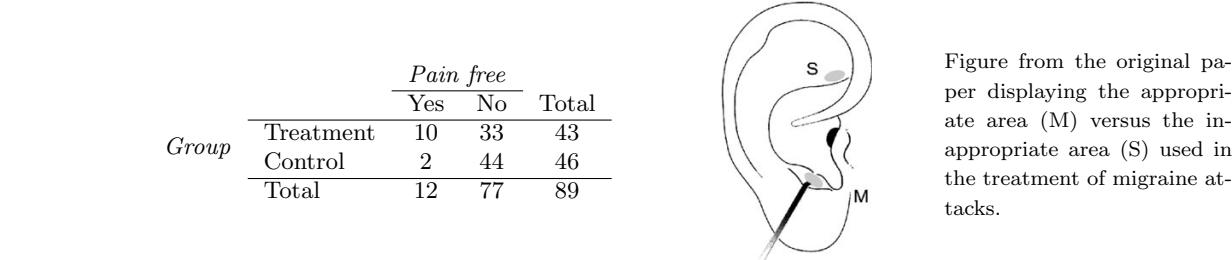
\includegraphics{_page_10_Figure_3.jpeg}

\begin{itemize}
\tightlist
\item
  inapropiado en términos de dar un efecto terapéutico sobre los ataques
  de migraña, ya que no tiene correlación somatotópica En el grupo B, la
  rama inferior del antélix fue (a) ¿Qué porcentaje de pacientes en el
  grupo de tratamiento estaban libres de dolor 24 horas después de
  recibir acupuntura?

  \begin{itemize}
  \tightlist
  \item
    probado repetidamente con el algómetro durante unos 30 s para (b)
    ¿Qué porcentaje estaban libres de dolor en el grupo de control?
  \item
    asegurarse de que no fuera sensible. En los mapas auriculares
    francés y chino, esta área corresponde a la representación (c) ¿En
    qué grupo un mayor porcentaje de pacientes se liberó del dolor 24
    horas después de recibir acupuntura?
  \end{itemize}
\item
  Materiales y métodos El estudio inscribió a 94 mujeres, diagnosticadas
  como migraña sin aura según la Clasificación Internacional de
  Trastornos de Cefalea {[}5{]}, que posteriormente fueron examinadas en
  el Centro de Cefaleas de Mujeres, Departamento de Ginecología. del
  nervio ciático (Fig. 1, área S) y se utiliza específicamente para
  tratar el dolor ciático. Se insertaron cuatro agujas en esta área, dos
  para cada oído. En todos los pacientes, la acupuntura auricular
  siempre fue realizada por un acupunturista experimentado. El análisis
  de los diarios que recopilaban datos de VAS fue realizado por un (d)
  Sus hallazgos hasta ahora podrían sugerir que la acupuntura es un
  tratamiento eficaz para las migrañas para todas las personas que
  sufren de migrañas. Sin embargo, esta no es la única conclusión
  posible que se puede extraer en función de sus hallazgos hasta ahora.
  ¿Cuál es otra posible explicación para la diferencia observada entre
  los porcentajes de pacientes que están libres de dolor 24 horas
  después de recibir acupuntura en los dos grupos?
\end{itemize}

ología y Obstetricia de la Universidad de Turín. Todas fueron incluidas
en el estudio durante un ataque de migraña siempre que hubiera comenzado
no más de 4 h antes. De acuerdo con una lista de aleatorización hecha
por computadora predeterminada, las pacientes elegibles fueron asignadas
aleatoria y ciegamente a los dos grupos siguientes: grupo A (n = 46)
(edad promedio 35,93 años, rango 15--60), grupo B (n = 48) (edad
promedio 33,2 años, rango 16--58). Antes de la inscripción, a cada
paciente se le pidió que diera un operador imparcial que no conocía el
grupo en el que estaba cada paciente. Los valores promedio de VAS en los
grupos A y B se calcularon en los diferentes momentos del estudio, y se
realizó una evaluación estadística de las diferencias entre los valores
obtenidos en T0, T1, T2, T3 y T4 en los dos grupos estudiados utilizando
un análisis de varianza (ANOVA) para medidas repetidas seguido de la
prueba t múltiple de Bonferroni para identificar la fuente de varianza.
\hyperref[page-383-2]{\textbf{1.2}} \textbf{Sinusitis y antibióticos,
Parte I.} Los investigadores que estudiaron el efecto del tratamiento
antibiótico para la sinusitis aguda en comparación con los tratamientos
sintomáticos asignaron aleatoriamente a 166 adultos diagnosticados con
sinusitis aguda a uno de dos grupos: tratamiento o control. Los
participantes del estudio recibieron un curso de 10 días de amoxicilina
(un antibiótico) o un placebo similar en apariencia y sabor. El placebo
consistió en tratamientos sintomáticos como acetaminofeno,
descongestionantes nasales, etc. Al final del período de 10 días, se
preguntó a los pacientes si experimentaban una mejora en los síntomas.
La distribución de las respuestas se resume a
continuación.\hyperref[page-10-1]{3}

\begin{longtable}[]{@{}
  >{\raggedright\arraybackslash}p{(\columnwidth - 8\tabcolsep) * \real{0.2000}}
  >{\raggedright\arraybackslash}p{(\columnwidth - 8\tabcolsep) * \real{0.2000}}
  >{\raggedright\arraybackslash}p{(\columnwidth - 8\tabcolsep) * \real{0.2000}}
  >{\raggedright\arraybackslash}p{(\columnwidth - 8\tabcolsep) * \real{0.2000}}
  >{\raggedright\arraybackslash}p{(\columnwidth - 8\tabcolsep) * \real{0.2000}}@{}}
\toprule\noalign{}
\begin{minipage}[b]{\linewidth}\raggedright
\end{minipage} & \begin{minipage}[b]{\linewidth}\raggedright
Además, para evaluar la diferencia entre el grupo By el grupo A, siempre
se realizó una prueba t para datos no pareados
\end{minipage} & \begin{minipage}[b]{\linewidth}\raggedright
Mejora autoinformada
\end{minipage} & \begin{minipage}[b]{\linewidth}\raggedright
\end{minipage} & \begin{minipage}[b]{\linewidth}\raggedright
\end{minipage} \\
\midrule\noalign{}
\endhead
\bottomrule\noalign{}
\endlastfoot
& se realizó para cada nivel de la variable `'tiempo'\,'. En el caso de
& & & \\
& & Sí & proporciones, se aplicó una prueba de Chi cuadrado. Todos los
análisisNose realizaron utilizando el Paquete Estadístico para lo Social
& Total \\
& Tratamiento & 66 & 19Software Sciences (SPSS). Todos los valores dados
en el & 85 \\
Grupo & ControlEl siguiente texto se informa como media aritmética
(±SEM). & 65 & 16 & 81 \\
& Total & 131 & 35 & 166 \\
\end{longtable}

\begin{itemize}
\tightlist
\item
  dolor cefálico prevalente. Si la prueba fue positiva y la reducción
  fue de al menos el 25\% con respecto a la base, una semi-Resultados
  (a) ¿Qué porcentaje de pacientes en el grupo de tratamiento
  experimentó una mejora en los síntomas?
\item
  aguja permanente (ASP SEDATELEC, Francia) se insertó después de 1 min.
  Por el contrario, si el dolor no disminuía Sólo 89 pacientes de todo
  el grupo de 94 (43 en el grupo A, 46 en el grupo B) completaron el
  experimento. Cuatro pacientes (b) ¿Qué porcentaje experimentó una
  mejora en los síntomas en el grupo de control?
\item
  después de 1 min, se desafió un punto sensible adicional en el se
  retiraron del estudio, porque experimentaron una (c) ¿En qué grupo un
  mayor porcentaje de pacientes experimentó una mejora en los síntomas?
\item
  misma área y así sucesivamente. Cuando los pacientes se dieron cuenta
  de una disminución inicial del dolor en todas las zonas de la cabeza
  afectadas, fueron invitados a usar una tarjeta de diario específica
  para calificar la intensidad del dolor con un VAS en los siguientes
  intervalos: después de 10 min (T1), después de 30 min (T2), después de
  60 min (T3), después de 120 min (T4) y después de 24 h (T5).
  exacerbación insoportable del dolor en el período anterior al último
  control a las 24 h (dos del grupo A y dos del grupo B) y fueron
  excluidos del análisis estadístico ya que solicitaron la extracción de
  las agujas. Una paciente del grupo A no dio su consentimiento para el
  implante de las agujas semipermanentes. En el grupo A, el número medio
  de (d) Sus hallazgos hasta ahora podrían sugerir una diferencia real
  en la eficacia de los tratamientos antibióticos y placebo para mejorar
  los síntomas de la sinusitis. Sin embargo, esta no es la única
  conclusión posible que se puede extraer en función de sus hallazgos
  hasta ahora. ¿Cuál es otra posible explicación para la diferencia
  observada entre los porcentajes de pacientes en los grupos de
  tratamiento con antibióticos y placebo que experimentan una mejora en
  los síntomas de la sinusitis?
\end{itemize}

2G. Allais et
al.~\href{http://www.openintro.org/redirect.php?go=textbook-acupuncture_migraine_2011&referrer=os4_pdf}{``Acupuntura
auricular en el tratamiento de los ataques de migraña: un ensayo
aleatorizado sobre la eficacia de}
\href{http://www.openintro.org/redirect.php?go=textbook-acupuncture_migraine_2011&referrer=os4_pdf}{puntos
de acupuntura apropiados versus inapropiados''}. En: Neurological Sci.
32.1 (2011), pp.~173--175.

3J.M. Garbutt et
al.~\href{http://www.openintro.org/redirect.php?go=textbook-amoxicillin_acute_rhinosinusitis_2012&referrer=os4_pdf}{``Amoxicilina
para la rinosinusitis aguda: un ensayo controlado aleatorizado''}. En:
JAMA: The Journal of the American Medical Association 307.7 (2012),
pp.~685--692.

\section{\texorpdfstring{\textbf{1.2 Conceptos básicos de
datos}}{1.2 Conceptos básicos de datos}}\label{conceptos-buxe1sicos-de-datos}

La organización y descripción eficaz de los datos es un primer paso en
la mayoría de los análisis. Esta sección presenta la matriz de datos
para organizar los datos, así como cierta terminología sobre las
diferentes formas de datos que se utilizarán a lo largo de este libro.

\section{\texorpdfstring{\textbf{1.2.1 Observaciones, variables y
matrices de
datos}}{1.2.1 Observaciones, variables y matrices de datos}}\label{observaciones-variables-y-matrices-de-datos}

La Figura \hyperref[page-11-1]{1.3} muestra las filas 1, 2, 3 y 50 de un
conjunto de datos de 50 préstamos seleccionados aleatoriamente ofrecidos
a través de Lending Club, que es una empresa de préstamos entre pares.
Estas observaciones se denominarán el conjunto de datos loan50.

Cada fila de la tabla representa un único préstamo. El nombre formal
para una fila es caso o unidad observacional. Las columnas representan
características, llamadas variables, para cada uno de los préstamos. Por
ejemplo, la primera fila representa un préstamo de \$22,000 con una tasa
de interés del 10.90\%, donde el prestatario tiene su sede en Nueva
Jersey (NJ) y tiene un ingreso de \$59,000.

\section{\texorpdfstring{\textbf{PRÁCTICA GUIADA
1.2}}{PRÁCTICA GUIADA 1.2}}\label{pruxe1ctica-guiada-1.2}

¿Cuál es la calificación del primer préstamo en la Figura
\hyperref[page-11-1]{1.3?} ¿Y cuál es el estado de propiedad de la
vivienda del prestatario para ese primer préstamo? Para estas preguntas
de Práctica Guiada, puedes verificar tu respuesta en la nota al
pie.\hyperref[page-11-2]{4}

En la práctica, es especialmente importante hacer preguntas aclaratorias
para asegurar que se comprendan aspectos importantes de los datos. Por
ejemplo, siempre es importante asegurarse de que sabemos lo que
significa cada variable y las unidades de medida. Las descripciones de
las variables loan50 se dan en la Figura \hyperref[page-11-3]{1.4.}

\begin{longtable}[]{@{}
  >{\raggedright\arraybackslash}p{(\columnwidth - 14\tabcolsep) * \real{0.1250}}
  >{\raggedright\arraybackslash}p{(\columnwidth - 14\tabcolsep) * \real{0.1250}}
  >{\raggedright\arraybackslash}p{(\columnwidth - 14\tabcolsep) * \real{0.1250}}
  >{\raggedright\arraybackslash}p{(\columnwidth - 14\tabcolsep) * \real{0.1250}}
  >{\raggedright\arraybackslash}p{(\columnwidth - 14\tabcolsep) * \real{0.1250}}
  >{\raggedright\arraybackslash}p{(\columnwidth - 14\tabcolsep) * \real{0.1250}}
  >{\raggedright\arraybackslash}p{(\columnwidth - 14\tabcolsep) * \real{0.1250}}
  >{\raggedright\arraybackslash}p{(\columnwidth - 14\tabcolsep) * \real{0.1250}}@{}}
\toprule\noalign{}
\begin{minipage}[b]{\linewidth}\raggedright
\end{minipage} & \begin{minipage}[b]{\linewidth}\raggedright
monto del préstamo
\end{minipage} & \begin{minipage}[b]{\linewidth}\raggedright
tasa de interés
\end{minipage} & \begin{minipage}[b]{\linewidth}\raggedright
plazo
\end{minipage} & \begin{minipage}[b]{\linewidth}\raggedright
calificación
\end{minipage} & \begin{minipage}[b]{\linewidth}\raggedright
estado
\end{minipage} & \begin{minipage}[b]{\linewidth}\raggedright
ingreso total
\end{minipage} & \begin{minipage}[b]{\linewidth}\raggedright
propiedad de vivienda
\end{minipage} \\
\midrule\noalign{}
\endhead
\bottomrule\noalign{}
\endlastfoot
1 & 22000 & 10.90 & 60.00 & B & NJ & 59000.00 & alquiler \\
2 & 6000 & 9.92 & 36.00 & B & CA & 60000.00 & alquiler \\
3 & 25000 & 26.30 & 36.00 & E & SC & 75000.00 & hipoteca \\
& & & & & & & \\
50 & 15000 & 6.08 & 36.00 & A & TX & 77500.00 & hipoteca \\
\end{longtable}

Figura 1.3: Cuatro filas de la matriz de datos loan50.

\begin{longtable}[]{@{}
  >{\raggedright\arraybackslash}p{(\columnwidth - 2\tabcolsep) * \real{0.5000}}
  >{\raggedright\arraybackslash}p{(\columnwidth - 2\tabcolsep) * \real{0.5000}}@{}}
\toprule\noalign{}
\begin{minipage}[b]{\linewidth}\raggedright
variable
\end{minipage} & \begin{minipage}[b]{\linewidth}\raggedright
descripción
\end{minipage} \\
\midrule\noalign{}
\endhead
\bottomrule\noalign{}
\endlastfoot
monto del préstamo & Monto del préstamo recibido, en dólares
estadounidenses. \\
tasa de interés & Tasa de interés del préstamo, en un porcentaje
anual. \\
plazo & La duración del préstamo, que siempre se establece como un
número entero de meses. \\
calificación & Calificación del préstamo, que toma valores de A a G y
representa la calidad del \\
& préstamo y su probabilidad de ser pagado. \\
estado & Estado de EE. UU. donde reside el prestatario. \\
ingreso total & Ingreso total del prestatario, incluyendo cualquier
segundo ingreso, en dólares estadounidenses. \\
propiedad de vivienda & Indica si la persona posee, posee pero tiene una
hipoteca o alquila. \\
\end{longtable}

Figura 1.4: Variables y sus descripciones para el conjunto de datos
loan50.

Los datos en la Figura \hyperref[page-11-1]{1.3} representan una matriz
de datos, que es una forma conveniente y común de organizar los datos,
especialmente si se recopilan datos en una hoja de cálculo. Cada fila de
una matriz de datos corresponde a un caso único (unidad de observación),
y cada columna corresponde a una variable.

4La calificación del préstamo es B, y el prestatario alquila su
residencia.

\section{1.2. FUNDAMENTOS DE LOS DATOS
13}\label{fundamentos-de-los-datos-13}

Al registrar datos, usa una matriz de datos a menos que tengas una muy
buena razón para usar una estructura diferente. Esta estructura permite
que se agreguen nuevos casos como filas o nuevas variables como nuevas
columnas.

\section{\texorpdfstring{\textbf{PRÁCTICA GUIADA
1.3}}{PRÁCTICA GUIADA 1.3}}\label{pruxe1ctica-guiada-1.3}

Las calificaciones de tareas, cuestionarios y exámenes en un curso a
menudo se registran en un libro de calificaciones que toma la forma de
una matriz de datos. ¿Cómo podría organizar los datos de las
calificaciones utilizando una matriz de datos?\hyperref[page-0-0]{5}

\paragraph{\texorpdfstring{\textbf{PRÁCTICA GUIADA
1.4}}{PRÁCTICA GUIADA 1.4}}\label{pruxe1ctica-guiada-1.4}

Consideramos datos de 3142 condados en los Estados Unidos, que incluyen
el nombre de cada condado, el estado donde reside, su población en 2017,
cómo cambió su población de 2010 a 2017, la tasa de pobreza y seis
características adicionales. ¿Cómo se podrían organizar estos datos en
una matriz de datos?\hyperref[page-12-0]{6}

Los datos descritos en la Práctica Guiada \hyperref[page-12-1]{1.4}
representan el conjunto de datos del condado, que se muestra como una
matriz de datos en la Figura \hyperref[page-13-0]{1.5.} Las variables se
resumen en la Figura \hyperref[page-13-1]{1.6.}

5Hay varias estrategias que se pueden seguir. Una estrategia común es
que cada estudiante esté representado por una fila y luego agregar una
columna para cada tarea, cuestionario o examen. Bajo esta configuración,
es fácil revisar una sola línea para comprender el historial de
calificaciones de un estudiante. También debe haber columnas para
incluir información del estudiante, como una columna para enumerar los
nombres de los estudiantes.

6Cada condado puede verse como un caso, y hay once datos registrados
para cada caso. Una tabla con 3142 filas y 11 columnas podría contener
estos datos, donde cada fila representa un condado y cada columna
representa una pieza de información particular.

\begin{longtable}[]{@{}
  >{\raggedright\arraybackslash}p{(\columnwidth - 22\tabcolsep) * \real{0.0833}}
  >{\raggedright\arraybackslash}p{(\columnwidth - 22\tabcolsep) * \real{0.0833}}
  >{\raggedright\arraybackslash}p{(\columnwidth - 22\tabcolsep) * \real{0.0833}}
  >{\raggedright\arraybackslash}p{(\columnwidth - 22\tabcolsep) * \real{0.0833}}
  >{\raggedright\arraybackslash}p{(\columnwidth - 22\tabcolsep) * \real{0.0833}}
  >{\raggedright\arraybackslash}p{(\columnwidth - 22\tabcolsep) * \real{0.0833}}
  >{\raggedright\arraybackslash}p{(\columnwidth - 22\tabcolsep) * \real{0.0833}}
  >{\raggedright\arraybackslash}p{(\columnwidth - 22\tabcolsep) * \real{0.0833}}
  >{\raggedright\arraybackslash}p{(\columnwidth - 22\tabcolsep) * \real{0.0833}}
  >{\raggedright\arraybackslash}p{(\columnwidth - 22\tabcolsep) * \real{0.0833}}
  >{\raggedright\arraybackslash}p{(\columnwidth - 22\tabcolsep) * \real{0.0833}}
  >{\raggedright\arraybackslash}p{(\columnwidth - 22\tabcolsep) * \real{0.0833}}@{}}
\toprule\noalign{}
\begin{minipage}[b]{\linewidth}\raggedright
\end{minipage} & \begin{minipage}[b]{\linewidth}\raggedright
nombre
\end{minipage} & \begin{minipage}[b]{\linewidth}\raggedright
estado
\end{minipage} & \begin{minipage}[b]{\linewidth}\raggedright
pob
\end{minipage} & \begin{minipage}[b]{\linewidth}\raggedright
cambiopob
\end{minipage} & \begin{minipage}[b]{\linewidth}\raggedright
pobreza
\end{minipage} & \begin{minipage}[b]{\linewidth}\raggedright
propiedad de vivienda
\end{minipage} & \begin{minipage}[b]{\linewidth}\raggedright
unidadmúltiple
\end{minipage} & \begin{minipage}[b]{\linewidth}\raggedright
tasadesempleo
\end{minipage} & \begin{minipage}[b]{\linewidth}\raggedright
metro
\end{minipage} & \begin{minipage}[b]{\linewidth}\raggedright
edumediana
\end{minipage} & \begin{minipage}[b]{\linewidth}\raggedright
ingresohogarmediana
\end{minipage} \\
\midrule\noalign{}
\endhead
\bottomrule\noalign{}
\endlastfoot
1 & Autauga & Alabama & 55504 & 1.48 & 13.7 & 77.5 & 7.2 & 3.86 & sí &
universidadalgunos & 55317 \\
2 & Baldwin & Alabama & 212628 & 9.19 & 11.8 & 76.7 & 22.6 & 3.99 & sí &
universidadalgunos & 52562 \\
3 & Barbour & Alabama & 25270 & -6.22 & 27.2 & 68.0 & 11.1 & 5.90 & no &
diplomahs & 33368 \\
4 & Bibb & Alabama & 22668 & 0.73 & 15.2 & 82.9 & 6.6 & 4.39 & sí &
diplomahs & 43404 \\
5 & Blount & Alabama & 58013 & 0.68 & 15.6 & 82.0 & 3.7 & 4.02 & sí &
diplomahs & 47412 \\
6 & Bullock & Alabama & 10309 & -2.28 & 28.5 & 76.9 & 9.9 & 4.93 & no &
diplomahs & 29655 \\
7 & Butler & Alabama & 19825 & -2.69 & 24.4 & 69.0 & 13.7 & 5.49 & no &
diplomahs & 36326 \\
8 & Calhoun & Alabama & 114728 & -1.51 & 18.6 & 70.7 & 14.3 & 4.93 & sí
& universidadalgunos & 43686 \\
9 & Chambers & Alabama & 33713 & -1.20 & 18.8 & 71.4 & 8.7 & 4.08 & no &
diplomahs & 37342 \\
10 & Cherokee & Alabama & 25857 & -0.60 & 16.1 & 77.5 & 4.3 & 4.05 & no
& diplomahs & 40041 \\
& & & & & & & & & & & \\
& & & & & & & & & & & \\
3142 & Weston & Wyoming & 6927 & -2.93 & 14.4 & 77.9 & 6.5 & 3.98 & no &
universidadalgunos & 59605 \\
& & & & & & & & & & & \\
\end{longtable}

Figura 1.5: Once filas del conjunto de datos del condado.

\begin{longtable}[]{@{}
  >{\raggedright\arraybackslash}p{(\columnwidth - 2\tabcolsep) * \real{0.5000}}
  >{\raggedright\arraybackslash}p{(\columnwidth - 2\tabcolsep) * \real{0.5000}}@{}}
\toprule\noalign{}
\begin{minipage}[b]{\linewidth}\raggedright
variable
\end{minipage} & \begin{minipage}[b]{\linewidth}\raggedright
descripción
\end{minipage} \\
\midrule\noalign{}
\endhead
\bottomrule\noalign{}
\endlastfoot
nombre & nombre.Condado \\
estado & Columbia.deDistritoeloreside,condadoeldondeEstado \\
pob & 2017.enPoblación \\
cambiopob &
valorelejemplo,Por2017.a2010depoblaciónlaencambioPorcentaje \\
&
1.48\%porincrementadocondadoesteparapoblaciónlasignificafilaprimeralaen1.48 \\
& 2017.a2010de \\
pobreza & pobreza.enpoblaciónladePorcentaje \\
propiedad de vivienda &
propietario,elconviveocasapropiasuenvivequepoblaciónladePorcentaje \\
& casa.lapropiaquienpadresconviviendoniñosp.ej. \\
unidadmúltiple &
mentos.apartep.ej.estructuras,multi-unidadensonqueunidadesviviendodePorcentaje \\
tasadesempleo & porciento.acomotasaDesempleo \\
metro & área.metropolitanaacontienecondadoelSi \\
edumediana &
diploma,hshs,debajoentrevaloratomarpuedequenivel,educaciónMediana \\
& licenciaturas.yuniversidad,algunos \\
ingresohogarmediana &
equivaleingresohogarmayor.adonde15condado,quienlosocupantesparaingresosudehogaringresototalMedianael \\
\end{longtable}

Figura 1.6: Variables y sus descripciones para el conjunto de datos del
condado.

\section{\texorpdfstring{\textbf{1.2.2 Tipos de
variables}}{1.2.2 Tipos de variables}}\label{tipos-de-variables}

Examine las variables tasa de desempleo, población, estado y educación
mediana en el conjunto de datos del condado. Cada una de estas variables
es inherentemente diferente de las otras tres, pero algunas comparten
ciertas características.

Primero considere la tasa de desempleo, que se dice que es una variable
numérica ya que puede tomar una amplia gama de valores numéricos, y es
sensato sumar, restar o tomar promedios con esos valores. Por otro lado,
no clasificaríamos una variable que informa los códigos de área
telefónica como numérica, ya que el promedio, la suma y la diferencia de
los códigos de área no tienen un significado claro.

La variable de población también es numérica, aunque parece ser un poco
diferente de la tasa de desempleo. Esta variable del conteo de la
población solo puede tomar números enteros no negativos (0, 1, 2,
\ldots). Por esta razón, se dice que la variable de población es
discreta, ya que solo puede tomar valores numéricos con saltos. Por otro
lado, se dice que la variable de la tasa de desempleo es continua.

La variable estado puede tomar hasta 51 valores después de contabilizar
Washington, DC: AL, AK, \ldots, y WY. Debido a que las respuestas en sí
mismas son categorías, estado se denomina variable categórica y los
valores posibles se denominan niveles de la variable.

Finalmente, considere la variable educación mediana, que describe el
nivel de educación mediano de los residentes del condado y toma los
valores por debajo de hs, diploma de hs, algo de universidad o
licenciatura en cada condado. Esta variable parece ser un híbrido: es
una variable categórica, pero los niveles tienen un ordenamiento
natural. Una variable con estas propiedades se denomina variable
ordinal, mientras que una variable categórica regular sin este tipo de
ordenamiento especial se denomina variable nominal. Para simplificar los
análisis, cualquier variable ordinal en este libro se tratará como una
variable categórica nominal (no ordenada).

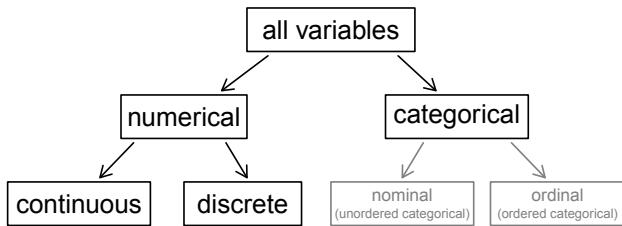
\includegraphics{_page_14_Figure_7.jpeg}

Figura 1.7: Desglose de las variables en sus respectivos tipos.

\section{\texorpdfstring{\textbf{EJEMPLO
1.5}}{EJEMPLO 1.5}}\label{ejemplo-1.5}

Se recolectaron datos sobre estudiantes en un curso de estadística. Se
registraron tres variables para cada estudiante: número de hermanos,
altura del estudiante y si el estudiante había tomado previamente un
curso de estadística. Clasifique cada una de las variables como numérica
continua, numérica discreta o categórica.

El número de hermanos y la altura del estudiante representan variables
numéricas. Debido a que el número de hermanos es un conteo, es discreto.
La altura varía continuamente, por lo que es una variable numérica
continua. La última variable clasifica a los estudiantes en dos
categorías: aquellos que han tomado y aquellos que no han tomado un
curso de estadística, lo que convierte a esta variable en categórica.

\section{\texorpdfstring{\textbf{PRÁCTICA GUIADA
1.6}}{PRÁCTICA GUIADA 1.6}}\label{pruxe1ctica-guiada-1.6}

Un experimento está evaluando la efectividad de un nuevo fármaco en el
tratamiento de las migrañas. Se utiliza una variable de grupo para
indicar el grupo experimental para cada paciente: tratamiento o control.
La variable num\_migrañas representa el número de migrañas que el
paciente experimentó durante un período de 3 meses. Clasifique cada
variable como numérica o categórica.\hyperref[page-14-0]{7}

7La variable de grupo solo puede tomar uno de dos nombres de grupo, lo
que la convierte en categórica. La variable num\_migrañas describe un
recuento del número de migrañas, que es un resultado donde la aritmética
básica es sensata, lo que significa que este es un resultado numérico;
más específicamente, dado que representa un recuento, num\_migrañas es
una variable numérica discreta.

\section{\texorpdfstring{\textbf{1.2.3 Relaciones entre
variables}}{1.2.3 Relaciones entre variables}}\label{relaciones-entre-variables}

Muchos análisis están motivados por un investigador que busca una
relación entre dos o más variables. A un científico social le gustaría
responder algunas de las siguientes preguntas:

\begin{itemize}
\tightlist
\item
  \begin{enumerate}
  \def\labelenumi{(\arabic{enumi})}
  \tightlist
  \item
    Si la propiedad de vivienda es inferior al promedio nacional en un
    condado, ¿el porcentaje de estructuras de unidades múltiples en ese
    condado tenderá a estar por encima o por debajo del promedio
    nacional?
  \end{enumerate}
\item
  \begin{enumerate}
  \def\labelenumi{(\arabic{enumi})}
  \setcounter{enumi}{1}
  \tightlist
  \item
    ¿Un aumento superior al promedio en la población del condado tiende
    a corresponder a condados con ingresos medios del hogar más altos o
    más bajos?
  \end{enumerate}
\item
  \begin{enumerate}
  \def\labelenumi{(\arabic{enumi})}
  \setcounter{enumi}{2}
  \tightlist
  \item
    ¿Qué tan útil es el nivel de educación medio como predictor del
    ingreso medio del hogar para los condados de EE. UU.?
  \end{enumerate}
\end{itemize}

Para responder a estas preguntas, se deben recopilar datos, como el
conjunto de datos del condado que se muestra en la Figura
\hyperref[page-13-0]{1.5.} El examen de las estadísticas resumidas
podría proporcionar información sobre cada una de las tres preguntas
sobre los condados. Además, se pueden utilizar gráficos para explorar
visualmente los datos.

Los diagramas de dispersión son un tipo de gráfico que se utiliza para
estudiar la relación entre dos variables numéricas. La Figura
\hyperref[page-15-0]{1.8} compara las variables propiedad de vivienda y
multi\_unidad, que es el porcentaje de unidades en estructuras de
unidades múltiples (por ejemplo, apartamentos, condominios). Cada punto
en el gráfico representa un solo condado. Por ejemplo, el punto
resaltado corresponde al condado 413 en el conjunto de datos del
condado: el condado de Chattahoochee, Georgia, que tiene el 39,4\% de
las unidades en estructuras de unidades múltiples y una tasa de
propiedad de vivienda del 31,3\%. El diagrama de dispersión sugiere una
relación entre las dos variables: los condados con una tasa más alta de
unidades múltiples tienden a tener tasas de propiedad de vivienda más
bajas. Podríamos hacer una lluvia de ideas sobre por qué existe esta
relación e investigar cada idea para determinar cuáles son las
explicaciones más razonables.

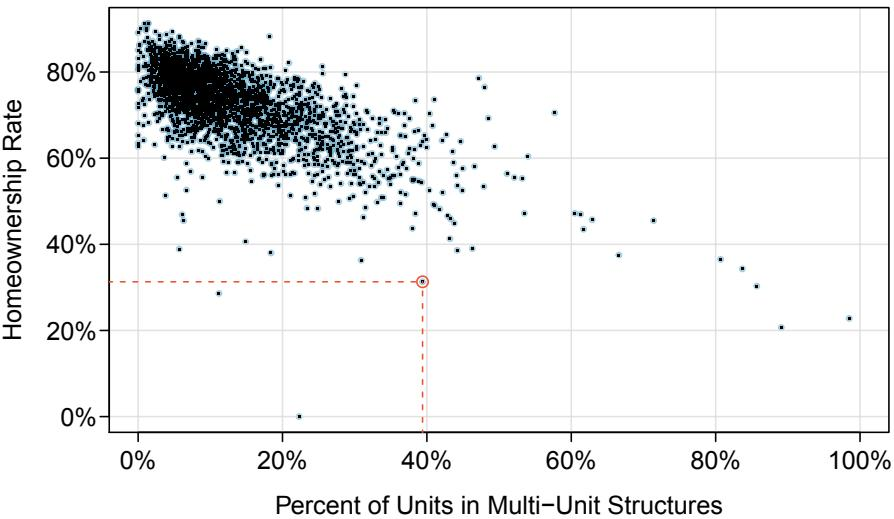
\includegraphics{_page_15_Figure_8.jpeg}

Figura 1.8: Un diagrama de dispersión de la propiedad de vivienda frente
al porcentaje de unidades que se encuentran en estructuras de unidades
múltiples para los condados de EE. UU. El punto resaltado representa el
condado de Chattahoochee, Georgia, que tiene una tasa de unidades
múltiples del 39,4\% y una tasa de propiedad de vivienda del 31,3\%.

Se dice que las tasas de multi\_unidad y propiedad de vivienda están
asociadas porque el gráfico muestra un patrón discernible. Cuando dos
variables muestran alguna conexión entre sí, se denominan variables
asociadas. Las variables asociadas también pueden denominarse variables
dependientes y viceversa.

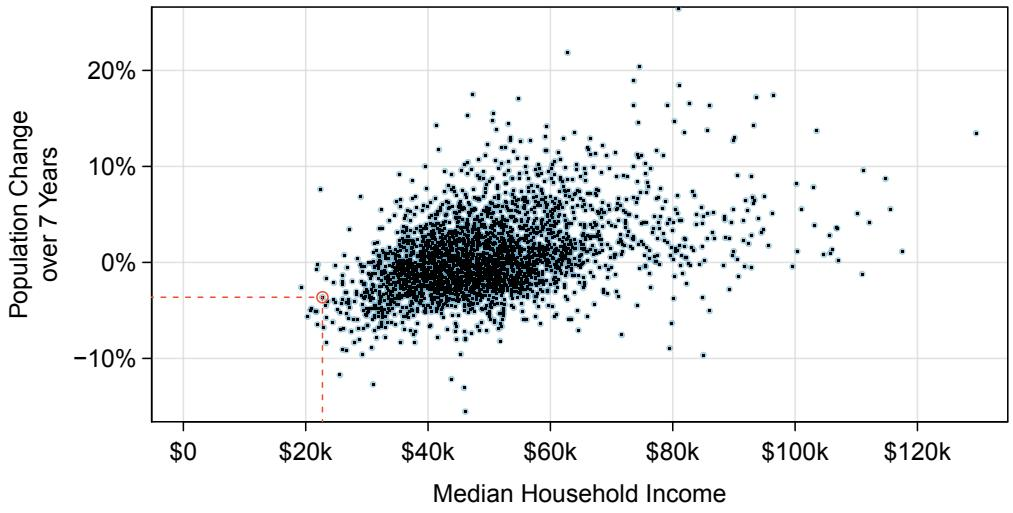
\includegraphics{_page_16_Figure_1.jpeg}

Figura 1.9: Un diagrama de dispersión que muestra el cambio de población
frente al ingreso medio del hogar. Se destaca el condado de Owsley de
Kentucky, que perdió el 3,63\% de su población entre 2010 y 2017 y tenía
un ingreso medio del hogar de \$22,736.

Examine las variables en el conjunto de datos loan50, que se describen
en la Figura \hyperref[page-11-3]{1.4 en la página 12.} Cree dos
preguntas sobre posibles relaciones entre variables en loan50 que sean
de su interés.\hyperref[page-16-0]{8}

\section{\texorpdfstring{\textbf{EJEMPLO
1.8}}{EJEMPLO 1.8}}\label{ejemplo-1.8}

Este ejemplo examina la relación entre el cambio de población de un
condado desde 2010 a 2017 y el ingreso medio por hogar, que se visualiza
como un diagrama de dispersión en la Figura \hyperref[page-16-1]{1.9.}
¿Están asociadas estas variables?

Cuanto mayor es el ingreso medio por hogar para un condado, mayor es el
crecimiento de la población observado para el condado. Si bien esta
tendencia no es cierta para todos los condados, la tendencia en el
gráfico es evidente. Dado que existe alguna relación entre las
variables, están asociadas.

Debido a que hay una tendencia a la baja en la Figura
\hyperref[page-15-0]{1.8} -- los condados con más unidades en
estructuras de unidades múltiples están asociados con una menor
propiedad de vivienda -- se dice que estas variables están negativamente
asociadas. Se muestra una asociación positiva en la relación entre el
ingreso medio por hogar y el cambio de población en la Figura
\hyperref[page-16-1]{1.9,} donde los condados con un ingreso medio por
hogar más alto tienden a tener tasas más altas de crecimiento de la
población.

Si dos variables no están asociadas, entonces se dice que son
independientes. Es decir, dos variables son independientes si no hay una
relación evidente entre las dos.

\paragraph{\texorpdfstring{\textbf{ASOCIADAS O INDEPENDIENTES, NO
AMBAS}}{ASOCIADAS O INDEPENDIENTES, NO AMBAS}}\label{asociadas-o-independientes-no-ambas}

Un par de variables están relacionadas de alguna manera (asociadas) o no
(independientes). Ningún par de variables es a la vez asociado e
independiente.

8Dos preguntas de ejemplo: (1) ¿Cuál es la relación entre el monto del
préstamo y el ingreso total? (2) Si el ingreso de alguien está por
encima del promedio, ¿su tasa de interés tenderá a estar por encima o
por debajo del promedio?

\section{\texorpdfstring{\textbf{1.2.4 Variables explicativas y de
respuesta}}{1.2.4 Variables explicativas y de respuesta}}\label{variables-explicativas-y-de-respuesta}

Cuando hacemos preguntas sobre la relación entre dos variables, a veces
también queremos determinar si el cambio en una variable causa un cambio
en la otra. Considere la siguiente reformulación de una pregunta
anterior sobre el conjunto de datos del condado:

Si hay un aumento en el ingreso medio por hogar en un condado, ¿esto
impulsa un aumento en su población?

En esta pregunta, estamos preguntando si una variable afecta a otra. Si
esta es nuestra creencia subyacente, entonces el ingreso medio por hogar
es la variable explicativa y el cambio de población es la variable de
respuesta en la relación hipotética.\hyperref[page-17-0]{9}

\section{\texorpdfstring{\textbf{VARIABLES EXPLICATIVAS Y DE
RESPUESTA}}{VARIABLES EXPLICATIVAS Y DE RESPUESTA}}\label{variables-explicativas-y-de-respuesta-1}

Cuando sospechamos que una variable podría afectar causalmente a otra,
etiquetamos la primera variable como la variable explicativa y la
segunda variable como la variable de respuesta.

\begin{quote}
la variable explicativa podría afectar a la variable de respuesta
\end{quote}

Para muchos pares de variables, no existe una relación hipotética, y
estas etiquetas no se aplicarían a ninguna de las variables en tales
casos.

Tenga en cuenta que el acto de etiquetar las variables de esta manera no
garantiza que exista una relación causal. Una evaluación formal para
verificar si una variable causa un cambio en otra requiere un
experimento.

\section{\texorpdfstring{\textbf{1.2.5 Introducción a los estudios
observacionales y
experimentos}}{1.2.5 Introducción a los estudios observacionales y experimentos}}\label{introducciuxf3n-a-los-estudios-observacionales-y-experimentos}

Existen dos tipos principales de recolección de datos: estudios
observacionales y experimentos.

Los investigadores realizan un estudio observacional cuando recolectan
datos de una manera que no interfiere directamente con la forma en que
surgen los datos. Por ejemplo, los investigadores pueden recolectar
información a través de encuestas, revisar registros médicos o de
empresas, o seguir a una cohorte de muchos individuos similares para
formular hipótesis sobre por qué podrían desarrollarse ciertas
enfermedades. En cada una de estas situaciones, los investigadores
simplemente observan los datos que surgen. En general, los estudios
observacionales pueden proporcionar evidencia de una asociación natural
entre variables, pero no pueden por sí solos mostrar una conexión
causal.

Cuando los investigadores quieren investigar la posibilidad de una
conexión causal, realizan un experimento. Por lo general, habrá una
variable explicativa y una variable de respuesta. Por ejemplo, podemos
sospechar que la administración de un fármaco reducirá la mortalidad en
pacientes con ataque cardíaco durante el año siguiente. Para verificar
si realmente existe una conexión causal entre la variable explicativa y
la respuesta, los investigadores recolectarán una muestra de individuos
y los dividirán en grupos. A los individuos de cada grupo se les asigna
un tratamiento. Cuando los individuos son asignados aleatoriamente a un
grupo, el experimento se denomina experimento aleatorizado. Por ejemplo,
cada paciente con ataque cardíaco en el ensayo del fármaco podría
asignarse aleatoriamente, tal vez lanzando una moneda al aire, en uno de
dos grupos: el primer grupo recibe un placebo (tratamiento falso) y el
segundo grupo recibe el fármaco. Consulte el estudio de caso en la
Sección \hyperref[page-8-0]{1.1} para ver otro ejemplo de un
experimento, aunque ese estudio no empleó un placebo.

\paragraph{\texorpdfstring{\textbf{ASOCIACIÓN} ̸=
\textbf{CAUSACIÓN}}{ASOCIACIÓN ̸= CAUSACIÓN}}\label{asociaciuxf3n-causaciuxf3n}

En general, la asociación no implica causalidad, y la causalidad solo
puede inferirse de un experimento aleatorizado.

9A veces, la variable explicativa se denomina variable independiente y
la variable de respuesta se denomina variable dependiente. Sin embargo,
esto se vuelve confuso ya que un par de variables podrían ser
independientes o dependientes, por lo que evitamos este lenguaje.

\textbf{Ejercicios} \hyperref[page-383-3]{\textbf{1.3}}
\textbf{Contaminación del aire y resultados del parto, componentes del
estudio.} Los investigadores recopilaron datos para examinar la relación
entre los contaminantes del aire y los partos prematuros en el sur de
California. Durante el estudio, los niveles de contaminación del aire se
midieron mediante estaciones de monitoreo de la calidad del aire.
Específicamente, se registraron los niveles de monóxido de carbono en
partes por millón, dióxido de nitrógeno y ozono en partes por cada cien
millones, y materia particulada gruesa (PM10) en µg/m3. Los datos de la
duración de la gestación se recopilaron en 143.196 partos entre los años
1989 y 1993, y la exposición a la contaminación del aire durante la
gestación se calculó para cada parto. El análisis sugirió que el aumento
de PM10 y, en menor medida, las concentraciones de CO pueden estar
asociados con la aparición de partos prematuros.\hyperref[page-18-0]{10}
- (a) Identifique la pregunta de investigación principal del estudio. -
(b) ¿Quiénes son los sujetos en este estudio, y cuántos están incluidos?
- (c) ¿Cuáles son las variables en el estudio? Identifique cada variable
como numérica o categórica. Si numérica, indique si la variable es
discreta o continua. Si categórica, indique si la variable es ordinal.
\hyperref[page-383-4]{\textbf{1.4}} \textbf{Método Buteyko, componentes
del estudio.} El método Buteyko es una técnica de respiración
superficial desarrollada por Konstantin Buteyko, un médico ruso, en
1952. La evidencia anecdótica sugiere que el método Buteyko puede
reducir los síntomas del asma y mejorar la calidad de vida. En un
estudio científico para determinar la efectividad de este método, los
investigadores reclutaron a 600 pacientes con asma de entre 18 y 69 años
que dependían de la medicación para el tratamiento del asma. Estos
pacientes fueron divididos aleatoriamente en dos grupos de
investigación: uno practicó el método Buteyko y el otro no. Los
pacientes fueron evaluados en calidad de vida, actividad, síntomas de
asma y reducción de medicación en una escala del 0 al 10. En promedio,
los participantes del grupo Buteyko experimentaron una reducción
significativa en los síntomas del asma y una mejora en la calidad de
vida.\hyperref[page-18-1]{11} - (a) Identifique la pregunta de
investigación principal del estudio. - (b) ¿Quiénes son los sujetos en
este estudio, y cuántos están incluidos? - (c) ¿Cuáles son las variables
en el estudio? Identifique cada variable como numérica o categórica. Si
numérica, indique si la variable es discreta o continua. Si categórica,
indique si la variable es ordinal. \hyperref[page-383-5]{\textbf{1.5}}
\textbf{Tramposos, componentes del estudio.} Los investigadores que
estudiaban la relación entre la honestidad, la edad y el autocontrol
llevaron a cabo un experimento con 160 niños de entre 5 y 15 años. Los
participantes informaron su edad, sexo y si eran hijo único o no. Los
investigadores le pidieron a cada niño que lanzara una moneda justa en
privado y que registrara el resultado (blanco o negro) en una hoja de
papel, y dijeron que solo recompensarían a los niños que informaran
blanco. Los hallazgos del estudio se pueden resumir de la siguiente
manera: ``La mitad de los estudiantes recibieron explícitamente la
instrucción de no hacer trampa y los demás no recibieron ninguna
instrucción explícita. En el grupo sin instrucciones, la probabilidad de
hacer trampa fue uniforme en los grupos según las características del
niño. En el grupo que recibió explícitamente la instrucción de no hacer
trampa, las niñas fueron menos propensas a hacer trampa, y mientras que
la tasa de hacer trampa no varió según la edad para los niños, disminuyó
con la edad para las niñas.''\hyperref[page-18-2]{12} - (a) Identifique
la pregunta de investigación principal del estudio. - (b) ¿Quiénes son
los sujetos en este estudio, y cuántos están incluidos? - (c) ¿Cuántas
variables se registraron para cada sujeto en el estudio para llegar a
estas conclusiones? Indique las variables y sus tipos.
\hyperref[page-383-6]{\textbf{1.6}} \textbf{Ladrones, componentes del
estudio.} En un estudio sobre la relación entre la clase socioeconómica
y el comportamiento poco ético, 129 estudiantes universitarios de la
Universidad de California en Berkeley fueron invitados a identificarse
como de clase social baja o alta al compararse con otros con el dinero
más (menos), la educación más (menos), y los trabajos más (menos)
respetados. También se les presentó un frasco de caramelos envueltos
individualmente e informaron que los caramelos eran para niños en un
laboratorio cercano, pero que podían tomar algunos si querían. Después
de completar algunas tareas sin relación, los participantes informaron
la cantidad de caramelos que habían tomado.\hyperref[page-19-0]{13} -
(a) Identifique la pregunta de investigación principal del estudio. -
(b) ¿Quiénes son los sujetos en este estudio, y cuántos están incluidos?
- (c) El estudio encontró que los estudiantes que se identificaron como
de clase alta tomaron más caramelos que otros. ¿Cuántas variables se
registraron para cada sujeto en el estudio para llegar a estas
conclusiones? Indique las variables y sus tipos.
\hyperref[page-383-7]{\textbf{1.7}} \textbf{Migraña y acupuntura, Parte
II.} El ejercicio \hyperref[page-10-2]{1.1} introdujo un estudio que
exploraba si la acupuntura tenía algún efecto en las migrañas. Los
investigadores llevaron a cabo un estudio controlado aleatorio en el que
los pacientes fueron asignados aleatoriamente a uno de dos grupos:
tratamiento o control. Los pacientes del grupo de tratamiento recibieron
acupuntura diseñada específicamente para tratar las migrañas. Los
pacientes del grupo de control recibieron acupuntura placebo (inserción
de agujas en lugares no acupunturales). 24 horas después de que los
pacientes recibieron acupuntura, se les preguntó si estaban libres de
dolor. ¿Cuáles son las variables explicativas y de respuesta en este
estudio? \hyperref[page-383-8]{\textbf{1.8}} \textbf{Sinusitis y
antibióticos, Parte II.} El ejercicio {[}1.2{]}(\#page-10-2{]} introdujo
un estudio que exploraba si los antibióticos tenían algún efecto en la
sinusitis. Los investigadores reclutaron a pacientes con sinusitis y los
asignaron aleatoriamente a un grupo que recibió antibióticos y a un
grupo que recibió un placebo. Después de una semana, los investigadores
evaluaron a los pacientes para ver si sus síntomas habían mejorado.
¿Cuáles son las variables explicativas y de respuesta en este estudio?
\hyperref[page-383-9]{\textbf{1.9}} \textbf{El efecto del ejercicio en
el estado de ánimo, componentes del estudio.} Un investigador está
interesado en determinar si el ejercicio afecta el estado de ánimo. El
investigador recluta a 30 voluntarios y les pide que informen su estado
de ánimo en una escala del 0 al 10, donde 0 es el estado de ánimo más
bajo y 10 es el estado de ánimo más alto. Luego, el investigador pide a
los participantes que hagan ejercicio durante 30 minutos y luego informa
su estado de ánimo nuevamente. ¿Cuál es la variable dependiente en este
estudio? \hyperref[page-383-10]{\textbf{1.10}} \textbf{El efecto de la
música en el rendimiento académico, componentes del estudio.} Un
profesor está interesado en determinar si la música afecta el
rendimiento académico. El profesor recluta a 50 estudiantes y les pide
que tomen un examen. Luego, el profesor pide a los estudiantes que
escuchen música durante 30 minutos y luego les pide que tomen otro
examen. ¿Cuál es la variable independiente en este estudio? 15Centro
Nacional de STEM,
\href{http://www.openintro.org/redirect.php?go=textbook-Stats4Schools_sokming&referrer=os4_pdf}{Grandes
conjuntos de datos de stats4schools.}

\section{1.2. BASES DE DATOS 21}\label{bases-de-datos-21}

\hyperref[page-383-11]{\textbf{1.11}} \textbf{Aeropuertos de EE.UU.} La
visualización a continuación muestra la distribución geográfica de los
aeropuertos en los Estados Unidos contiguos y Washington, DC. Esta
visualización se construyó a partir de un conjunto de datos donde cada
observación es un aeropuerto.\hyperref[page-20-0]{16}

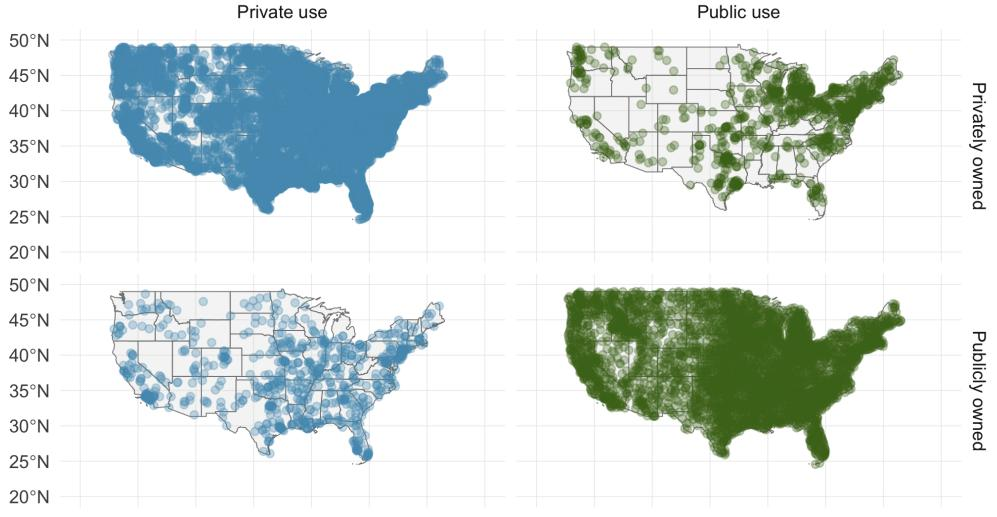
\includegraphics{_page_20_Figure_2.jpeg}

\begin{itemize}
\tightlist
\item
\item
  \begin{enumerate}
  \def\labelenumi{(\alph{enumi})}
  \tightlist
  \item
    Enumere las variables utilizadas para crear esta visualización.
  \end{enumerate}
\item
  \begin{enumerate}
  \def\labelenumi{(\alph{enumi})}
  \setcounter{enumi}{1}
  \tightlist
  \item
    Indique si cada variable en el estudio es numérica o categórica. Si
    es numérica, identifique si es continua o discreta. Si es
    categórica, indique si la variable es ordinal.
  \end{enumerate}
\end{itemize}

\hyperref[page-383-12]{\textbf{1.12}} \textbf{Votos de la ONU.} La
visualización a continuación muestra los patrones de votación en los
Estados Unidos, Canadá y México en la Asamblea General de las Naciones
Unidas sobre una variedad de temas. Específicamente, para un año dado
entre 1946 y 2015, muestra el porcentaje de votaciones nominales en las
que el país votó sí para cada tema. Esta visualización se construyó a
partir de un conjunto de datos donde cada observación es un par
país/año.\hyperref[page-20-1]{17}

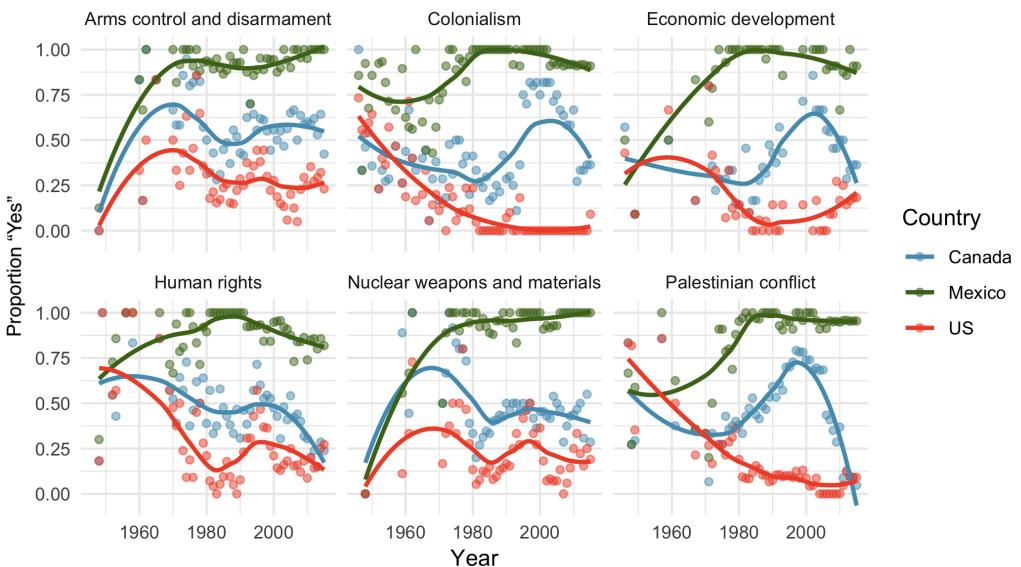
\includegraphics{_page_20_Figure_7.jpeg}

\begin{itemize}
\tightlist
\item
  \begin{enumerate}
  \def\labelenumi{(\alph{enumi})}
  \tightlist
  \item
    Enumere las variables utilizadas para crear esta visualización.
  \end{enumerate}
\item
  \begin{enumerate}
  \def\labelenumi{(\alph{enumi})}
  \setcounter{enumi}{1}
  \tightlist
  \item
    Indique si cada variable en el estudio es numérica o categórica. Si
    es numérica, identifique si es continua o discreta. Si es
    categórica, indique si la variable es ordinal.
  \end{enumerate}
\end{itemize}

16Administración Federal de Aviación,
\href{http://www.openintro.org/redirect.php?go=textbook-FAA_airports&referrer=os4_pdf}{www.faa.gov/airports/airport}
safety/airportdata 5010.

17David Robinson. unvotes: Datos de votación de la Asamblea General de
las Naciones Unidas. Paquete R versión 0.2.0. 2017. url:
\url{https://CRAN.R-project.org/package=unvotes}.

\section{\texorpdfstring{\textbf{1.3 Principios y estrategias de
muestreo}}{1.3 Principios y estrategias de muestreo}}\label{principios-y-estrategias-de-muestreo}

El primer paso para llevar a cabo una investigación es identificar los
temas o preguntas que se investigarán. Una pregunta de investigación
claramente definida es útil para identificar qué sujetos o casos deben
estudiarse y qué variables son importantes. También es importante
considerar cómo se recopilan los datos para que sean confiables y ayuden
a lograr los objetivos de la investigación.

\section{\texorpdfstring{\textbf{1.3.1 Poblaciones y
muestras}}{1.3.1 Poblaciones y muestras}}\label{poblaciones-y-muestras}

Considera las siguientes tres preguntas de investigación:

\begin{itemize}
\item
  \begin{enumerate}
  \def\labelenumi{\arabic{enumi}.}
  \tightlist
  \item
    ¿Cuál es el contenido promedio de mercurio en el pez espada en el
    Océano Atlántico?
  \end{enumerate}
\item
  2. Durante los últimos 5 años, ¿cuál es el tiempo promedio para
  completar una licenciatura para los estudiantes de Duke?
\item
  3. ¿Un nuevo fármaco reduce el número de muertes en pacientes con
  enfermedad cardíaca grave?
\end{itemize}

Cada pregunta de investigación se refiere a una población objetivo. En
la primera pregunta, la población objetivo son todos los peces espada en
el Océano Atlántico, y cada pez representa un caso. A menudo, es
demasiado costoso recopilar datos para cada caso en una población. En
cambio, se toma una muestra. Una muestra representa un subconjunto de
los casos y a menudo es una pequeña fracción de la población. Por
ejemplo, se podrían seleccionar 60 peces espada (o algún otro número) de
la población, y estos datos de muestra podrían usarse para proporcionar
una estimación del promedio de la población y responder a la pregunta de
investigación.

\section{\texorpdfstring{\textbf{PRÁCTICA GUIADA
1.9}}{PRÁCTICA GUIADA 1.9}}\label{pruxe1ctica-guiada-1.9}

Para la segunda y tercera pregunta anteriores, identifica la población
objetivo y qué representa un caso individual.\hyperref[page-21-1]{18}

\section{\texorpdfstring{\textbf{1.3.2 Evidencia
anecdótica}}{1.3.2 Evidencia anecdótica}}\label{evidencia-anecduxf3tica}

Considera las siguientes posibles respuestas a las tres preguntas de
investigación:

\begin{itemize}
\tightlist
\item
  \begin{enumerate}
  \def\labelenumi{\arabic{enumi}.}
  \tightlist
  \item
    Un hombre en las noticias se intoxicó con mercurio por comer pez
    espada, por lo que la concentración promedio de mercurio en el pez
    espada debe ser peligrosamente alta.
  \end{enumerate}
\item
  \begin{enumerate}
  \def\labelenumi{\arabic{enumi}.}
  \setcounter{enumi}{1}
  \tightlist
  \item
    Conocí a dos estudiantes que tardaron más de 7 años en graduarse de
    Duke, por lo que debe tomar más tiempo graduarse en Duke que en
    muchas otras universidades.
  \end{enumerate}
\item
  \begin{enumerate}
  \def\labelenumi{\arabic{enumi}.}
  \setcounter{enumi}{2}
  \tightlist
  \item
    El papá de mi amigo tuvo un ataque al corazón y murió después de que
    le dieron un nuevo medicamento para la enfermedad cardíaca, por lo
    que el medicamento no debe funcionar.
  \end{enumerate}
\end{itemize}

Cada conclusión se basa en datos. Sin embargo, hay dos problemas.
Primero, los datos solo representan uno o dos casos. Segundo, y más
importante, no está claro si estos casos son realmente representativos
de la población. Los datos recopilados de esta manera descuidada se
denominan evidencia anecdótica.

\paragraph{\texorpdfstring{\textbf{EVIDENCIA
ANECDÓTICA}}{EVIDENCIA ANECDÓTICA}}\label{evidencia-anecduxf3tica-1}

Ten cuidado con los datos recopilados de forma descuidada. Tal evidencia
puede ser verdadera y verificable, pero solo puede representar casos
extraordinarios.

18\hyperref[page-21-2]{(2)} La primera pregunta solo es relevante para
los estudiantes que completan su título; el promedio no se puede
calcular utilizando a un estudiante que nunca terminó su título. Por lo
tanto, solo los estudiantes de pregrado de Duke que se graduaron en los
últimos cinco años representan casos en la población en consideración.
Cada uno de estos estudiantes es un caso individual.
\hyperref[page-21-3]{(3)} Una persona con una enfermedad cardíaca grave
representa un caso. La población incluye a todas las personas con una
enfermedad cardíaca grave.

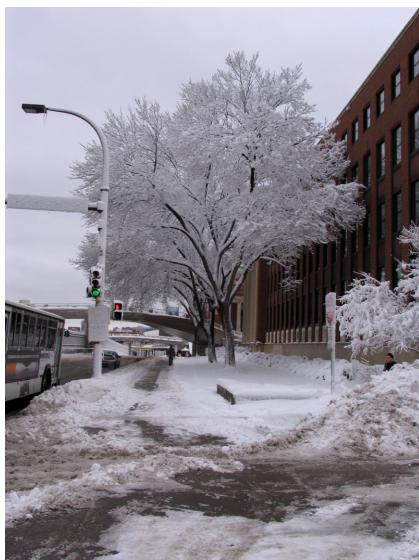
\includegraphics{_page_22_Picture_1.jpeg}

Figura 1.10: En febrero de 2010, algunos expertos de los medios citaron
una gran tormenta de nieve como evidencia válida contra el calentamiento
global. Como señaló el comediante Jon Stewart, ``Es una tormenta, en una
región, de un país''.

La evidencia anecdótica típicamente se compone de casos inusuales que
recordamos en función de sus características sorprendentes. Por ejemplo,
es más probable que recordemos a las dos personas que conocimos que
tardaron 7 años en graduarse que a las otras seis que se graduaron en
cuatro años. En lugar de observar los casos más inusuales, deberíamos
examinar una muestra de muchos casos que representen a la población.

\section{\texorpdfstring{\textbf{1.3.3 Muestreo de una
población}}{1.3.3 Muestreo de una población}}\label{muestreo-de-una-poblaciuxf3n}

Podríamos intentar estimar el tiempo hasta la graduación de los
estudiantes de pregrado de Duke en los últimos 5 años recolectando una
muestra de estudiantes. Todos los graduados en los últimos 5 años
representan la población, y los graduados que son seleccionados para su
revisión se denominan colectivamente la muestra. En general, siempre
buscamos seleccionar aleatoriamente una muestra de una población. El
tipo más básico de selección aleatoria es equivalente a cómo se realizan
las rifas. Por ejemplo, al seleccionar graduados, podríamos escribir el
nombre de cada graduado en un boleto de rifa y sacar 100 boletos. Los
nombres seleccionados representarían una muestra aleatoria de 100
graduados. Elegimos muestras aleatoriamente para reducir la posibilidad
de introducir sesgos.

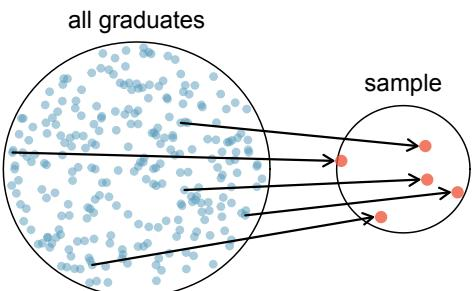
\includegraphics{_page_22_Figure_6.jpeg}

Figura 1.11: En este gráfico, cinco graduados son seleccionados
aleatoriamente de la población para ser incluidos en la muestra.

\section{\texorpdfstring{\textbf{EJEMPLO
1.10}}{EJEMPLO 1.10}}\label{ejemplo-1.10}

Supongamos que le pedimos a un estudiante que se especializa en
nutrición que seleccione a varios graduados para el estudio. ¿Qué tipo
de estudiantes crees que podría reunir? ¿Crees que su muestra sería
representativa de todos los graduados?

Tal vez elegiría un número desproporcionado de graduados de campos
relacionados con la salud. O tal vez su selección sería una buena
representación de la población. Al seleccionar muestras a mano, corremos
el riesgo de elegir una muestra sesgada, incluso si su sesgo no es
intencionado.

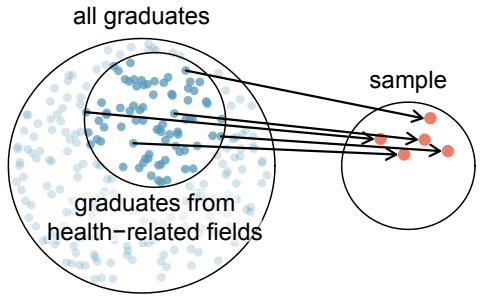
\includegraphics{_page_23_Figure_1.jpeg}

Figura 1.12: Si se le pide que elija una muestra de graduados, un
estudiante de nutrición podría elegir inadvertidamente un número
desproporcionado de graduados de carreras relacionadas con la salud.

Si a alguien se le permitiera elegir exactamente qué graduados se
incluyen en la muestra, es muy posible que la muestra se inclinara hacia
los intereses de esa persona, lo que puede ser completamente
involuntario. Esto introduce sesgo en una muestra. El muestreo aleatorio
ayuda a resolver este problema. La muestra aleatoria más básica se llama
muestra aleatoria simple, que es equivalente a usar una rifa para
seleccionar casos. Esto significa que cada caso en la población tiene la
misma probabilidad de ser incluido y no hay una conexión implícita entre
los casos en la muestra.

El acto de tomar una muestra aleatoria simple ayuda a minimizar el
sesgo. Sin embargo, el sesgo puede surgir de otras maneras. Incluso
cuando las personas son elegidas al azar, por ejemplo, para encuestas,
se debe tener precaución si la tasa de no respuesta es alta. Por
ejemplo, si solo el 30\% de las personas seleccionadas al azar para una
encuesta responden, entonces no está claro si los resultados son
representativos de toda la población. Este sesgo de no respuesta puede
sesgar los resultados.

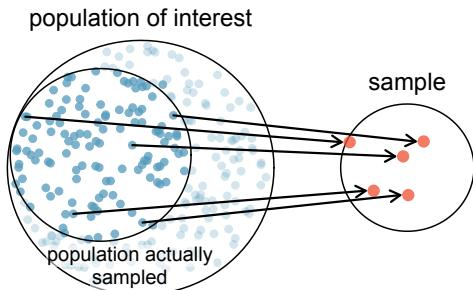
\includegraphics{_page_23_Figure_5.jpeg}

Figura 1.13: Debido a la posibilidad de no respuesta, los estudios de
encuestas pueden llegar solo a un cierto grupo dentro de la población.
Es difícil, y muchas veces imposible, solucionar por completo este
problema.

Otro error común es una muestra de conveniencia, donde los individuos
que son fácilmente accesibles tienen más probabilidades de ser incluidos
en la muestra. Por ejemplo, si una encuesta política se realiza
deteniendo a personas que caminan en el Bronx, esto no representará a
toda la ciudad de Nueva York. A menudo es difícil discernir qué
subpoblación representa una muestra de conveniencia.

\paragraph{\texorpdfstring{\textbf{PRÁCTICA GUIADA
1.11}}{PRÁCTICA GUIADA 1.11}}\label{pruxe1ctica-guiada-1.11}

Podemos acceder fácilmente a las calificaciones de productos, vendedores
y empresas a través de sitios web. Estas calificaciones se basan
únicamente en aquellas personas que se esfuerzan por proporcionar una
calificación. Si el 50\% de las reseñas en línea de un producto son
negativas, ¿cree que esto significa que el 50\% de los compradores están
insatisfechos con el producto?\hyperref[page-23-0]{19}

19Las respuestas variarán. A partir de nuestras propias experiencias
anecdóticas, creemos que las personas tienden a despotricar más sobre
los productos que no cumplieron con las expectativas que a entusiasmarse
con aquellos que funcionan como se esperaba. Por esta razón, sospechamos
que existe un sesgo negativo en las calificaciones de productos en
sitios como Amazon. Sin embargo, dado que nuestras experiencias pueden
no ser representativas, también mantenemos una mente abierta.

\section{\texorpdfstring{\textbf{1.3.4 Estudios
observacionales}}{1.3.4 Estudios observacionales}}\label{estudios-observacionales}

Los datos donde no se ha aplicado explícitamente ningún tratamiento (o
se ha retenido explícitamente) se denominan datos observacionales. Por
ejemplo, los datos de préstamos y los datos del condado descritos en la
Sección \hyperref[page-11-0]{1.2} son ejemplos de datos observacionales.
Hacer conclusiones causales basadas en experimentos suele ser razonable.
Sin embargo, hacer las mismas conclusiones causales basadas en datos
observacionales puede ser traicionero y no se recomienda. Por lo tanto,
los estudios observacionales generalmente solo son suficientes para
mostrar asociaciones o formar hipótesis que luego verificamos utilizando
experimentos.

\paragraph{\texorpdfstring{\textbf{PRÁCTICA GUIADA
1.12}}{PRÁCTICA GUIADA 1.12}}\label{pruxe1ctica-guiada-1.12}

Supongamos que un estudio observacional rastreó el uso de protector
solar y el cáncer de piel, y se descubrió que cuanto más protector solar
usaba alguien, más probable era que la persona tuviera cáncer de piel.
¿Significa esto que el protector solar causa cáncer de
piel?\hyperref[page-24-0]{20}

Algunas investigaciones previas nos dicen que usar protector solar en
realidad reduce el riesgo de cáncer de piel, por lo que tal vez haya
otra variable que pueda explicar esta hipotética asociación entre el uso
de protector solar y el cáncer de piel. Una pieza importante de
información que está ausente es la exposición al sol. Si alguien está
expuesto al sol todo el día, es más probable que use protector solar y
que le dé cáncer de piel. La exposición al sol no se tiene en cuenta en
la simple investigación.

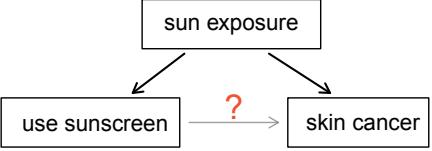
\includegraphics{_page_24_Figure_6.jpeg}

La exposición al sol es lo que se llama una variable de
confusión,\hyperref[page-24-1]{21} que es una variable que está
correlacionada tanto con las variables explicativas como con las
variables de respuesta. Si bien un método para justificar la elaboración
de conclusiones causales a partir de estudios observacionales es agotar
la búsqueda de variables de confusión, no hay garantía de que todas las
variables de confusión puedan examinarse o medirse.

\paragraph{\texorpdfstring{\textbf{PRÁCTICA GUIADA
1.13}}{PRÁCTICA GUIADA 1.13}}\label{pruxe1ctica-guiada-1.13}

La Figura \hyperref[page-15-0]{1.8} muestra una asociación negativa
entre la tasa de propiedad de vivienda y el porcentaje de estructuras de
unidades múltiples en un condado. Sin embargo, no es razonable concluir
que existe una relación causal entre las dos variables. Sugiera una
variable que pueda explicar la relación
negativa.\hyperref[page-24-2]{22}

Los estudios observacionales se presentan en dos formas: estudios
prospectivos y retrospectivos. Un estudio prospectivo identifica a los
individuos y recopila información a medida que se desarrollan los
eventos. Por ejemplo, los investigadores médicos pueden identificar y
seguir a un grupo de pacientes durante muchos años para evaluar las
posibles influencias del comportamiento en el riesgo de cáncer. Un
ejemplo de tal estudio es el Estudio de Salud de las Enfermeras, que
comenzó en 1976 y se amplió en 1989. Este estudio prospectivo recluta
enfermeras registradas y luego recopila datos de ellas mediante
cuestionarios. Los estudios retrospectivos recopilan datos después de
que los eventos han tenido lugar, por ejemplo, los investigadores pueden
revisar eventos pasados \hspace{0pt}\hspace{0pt}en registros médicos.
Algunos conjuntos de datos pueden contener variables recopiladas tanto
prospectiva como retrospectivamente.

\section{\texorpdfstring{\textbf{1.3.5 Cuatro métodos de
muestreo}}{1.3.5 Cuatro métodos de muestreo}}\label{cuatro-muxe9todos-de-muestreo}

Casi todos los métodos estadísticos se basan en la noción de
aleatoriedad implícita. Si los datos observacionales no se recopilan de
un marco aleatorio de una población, estos métodos estadísticos -- las
estimaciones y los errores asociados con las estimaciones -- no son
confiables. Aquí consideramos cuatro técnicas de muestreo aleatorio:
muestreo simple, estratificado, por conglomerados y multietápico. Las
figuras \hyperref[page-25-0]{1.14} y \hyperref[page-27-0]{1.15}
proporcionan representaciones gráficas de estas técnicas.

20No.~Consulte el párrafo posterior al ejercicio para obtener una
explicación.

21También llamada variable latente, factor de confusión o confusor.

22Las respuestas variarán. La densidad de población puede ser
importante. Si un condado es muy denso, esto puede requerir que una
mayor fracción de residentes viva en estructuras de varias unidades.
Además, la alta densidad puede contribuir al aumento del valor de las
propiedades, lo que hace que la propiedad de la vivienda sea inviable
para muchos residentes.

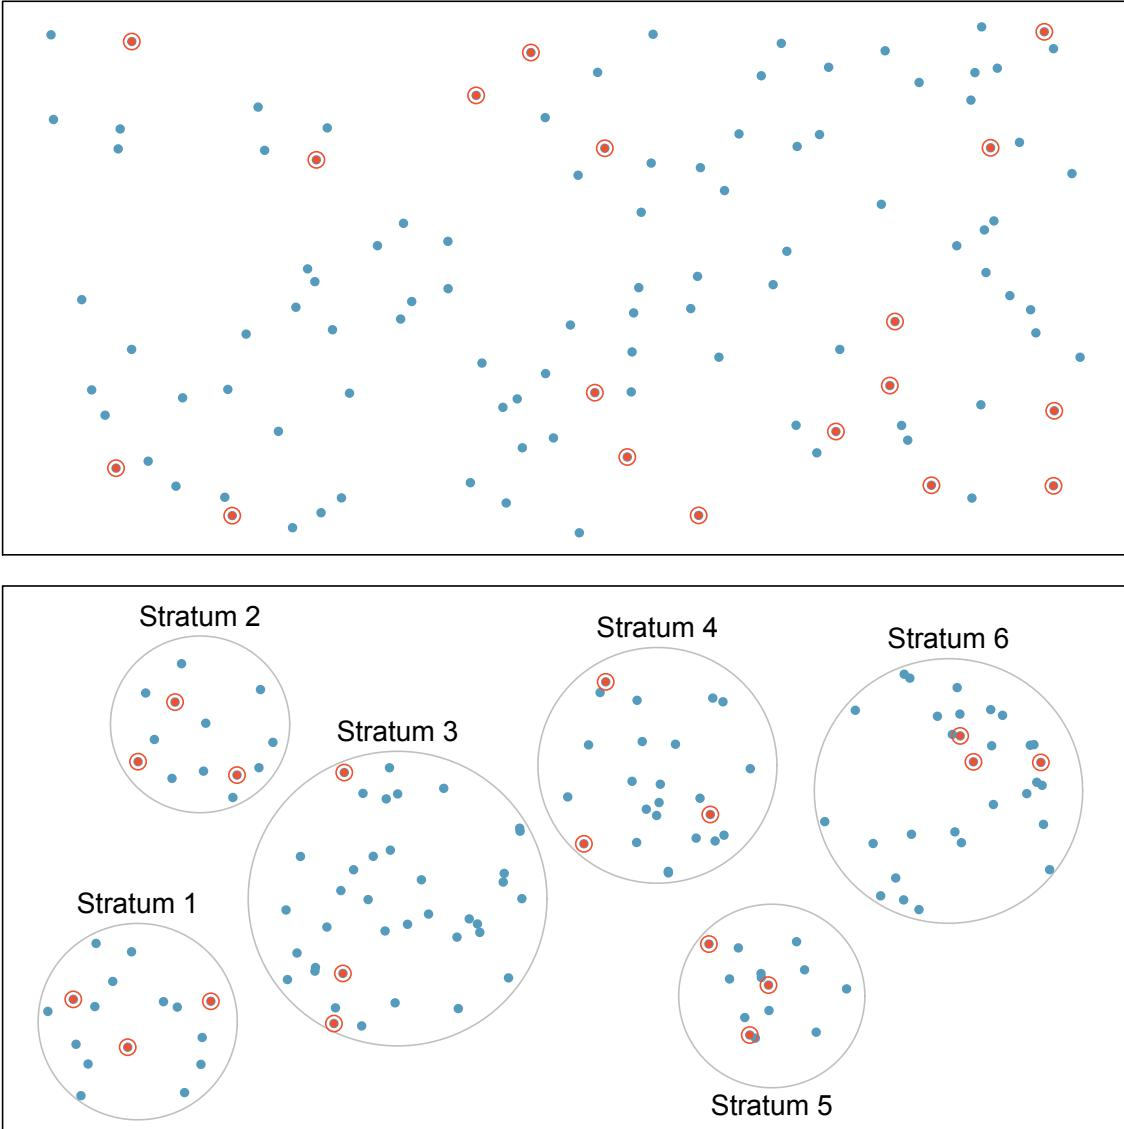
\includegraphics{_page_25_Figure_1.jpeg}

Figura 1.14: Ejemplos de muestreo aleatorio simple y estratificado. En
el panel superior, se utilizó el muestreo aleatorio simple para
seleccionar aleatoriamente los 18 casos. En el panel inferior, se
utilizó el muestreo estratificado: los casos se agruparon en estratos,
luego se empleó el muestreo aleatorio simple dentro de cada estrato.

\section{1.3. PRINCIPIOS Y ESTRATEGIAS DE MUESTREO
27}\label{principios-y-estrategias-de-muestreo-27}

El muestreo aleatorio simple es probablemente la forma más intuitiva de
muestreo aleatorio. Considere los salarios de los jugadores de las
Grandes Ligas de Béisbol (MLB), donde cada jugador es miembro de uno de
los 30 equipos de la liga. Para tomar una muestra aleatoria simple de
120 jugadores de béisbol y sus salarios, podríamos escribir los nombres
de los varios cientos de jugadores de esa temporada en trozos de papel,
dejar caer los trozos en un balde, agitar el balde hasta que estemos
seguros de que los nombres están mezclados, luego sacar los trozos hasta
que tengamos la muestra de 120 jugadores. En general, una muestra se
conoce como ``aleatoria simple'' si cada caso en la población tiene la
misma probabilidad de ser incluido en la muestra final y saber que un
caso está incluido en una muestra no proporciona información útil sobre
qué otros casos están incluidos.

El muestreo estratificado es una estrategia de muestreo de divide y
vencerás. La población se divide en grupos llamados estratos. Los
estratos se eligen de modo que los casos similares se agrupen, luego se
emplea un segundo método de muestreo, generalmente el muestreo aleatorio
simple, dentro de cada estrato. En el ejemplo del salario del béisbol,
los equipos podrían representar los estratos, ya que algunos equipos
tienen mucho más dinero (¡hasta 4 veces más!). Entonces podríamos
muestrear aleatoriamente a 4 jugadores de cada equipo para un total de
120 jugadores.

El muestreo estratificado es especialmente útil cuando los casos en cada
estrato son muy similares con respecto al resultado de interés. La
desventaja es que analizar datos de una muestra estratificada es una
tarea más compleja que analizar datos de una muestra aleatoria simple.
Los métodos de análisis introducidos en este libro deberían ampliarse
para analizar los datos recopilados mediante el muestreo estratificado.

\subsection{\texorpdfstring{\textbf{EJEMPLO
1.14}}{EJEMPLO 1.14}}\label{ejemplo-1.14}

¿Por qué sería bueno que los casos dentro de cada estrato fueran muy
similares?

Podríamos obtener una estimación más estable para la subpoblación en un
estrato si los casos son muy similares, lo que conduciría a estimaciones
más precisas dentro de cada grupo. Cuando combinamos estas estimaciones
en una sola estimación para la población completa, esa estimación de la
población tenderá a ser más precisa, ya que cada estimación de grupo
individual es en sí misma más precisa.

En un muestreo por conglomerados, dividimos la población en muchos
grupos, llamados conglomerados. Luego muestreamos un número fijo de
conglomerados e incluimos todas las observaciones de cada uno de esos
conglomerados en la muestra. Un muestreo multietápico es como un
muestreo por conglomerados, pero en lugar de mantener todas las
observaciones en cada conglomerado, recopilamos una muestra aleatoria
dentro de cada conglomerado seleccionado.

A veces, el muestreo por conglomerados o multietápico puede ser más
económico que las técnicas de muestreo alternativas. Además, a
diferencia del muestreo estratificado, estos enfoques son más útiles
cuando hay mucha variabilidad de caso a caso dentro de un conglomerado,
pero los conglomerados en sí mismos no se ven muy diferentes entre sí.
Por ejemplo, si los vecindarios representaran conglomerados, entonces el
muestreo por conglomerados o multietápico funciona mejor cuando los
vecindarios son muy diversos. Una desventaja de estos métodos es que
normalmente se requieren técnicas más avanzadas para analizar los datos,
aunque los métodos de este libro se pueden ampliar para manejar tales
datos.

\paragraph{\texorpdfstring{\textbf{EJEMPLO
1.15}}{EJEMPLO 1.15}}\label{ejemplo-1.15}

Supongamos que estamos interesados en estimar la tasa de malaria en una
porción densamente tropical de la Indonesia rural. Nos enteramos de que
hay 30 aldeas en esa parte de la jungla indonesia, cada una más o menos
similar a la siguiente. Nuestro objetivo es examinar a 150 personas para
detectar malaria. ¿Qué método de muestreo se debe emplear?

Un muestreo aleatorio simple probablemente extraerá individuos de las 30
aldeas, lo que podría hacer que la recopilación de datos sea
extremadamente costosa. El muestreo estratificado sería un desafío ya
que no está claro cómo construiríamos estratos de individuos similares.
Sin embargo, el muestreo por conglomerados o el muestreo multietápico
parecen ser muy buenas ideas. Si decidiéramos utilizar el muestreo
multietápico, podríamos seleccionar aleatoriamente la mitad de las
aldeas y luego seleccionar aleatoriamente a 10 personas de cada una.
Esto probablemente reduciría sustancialmente nuestros costos de
recopilación de datos en comparación con un muestreo aleatorio simple, y
el muestreo por conglomerados aún nos brindaría información confiable,
incluso si tuviéramos que analizar los datos con métodos un poco más
avanzados de los que discutimos en este libro.

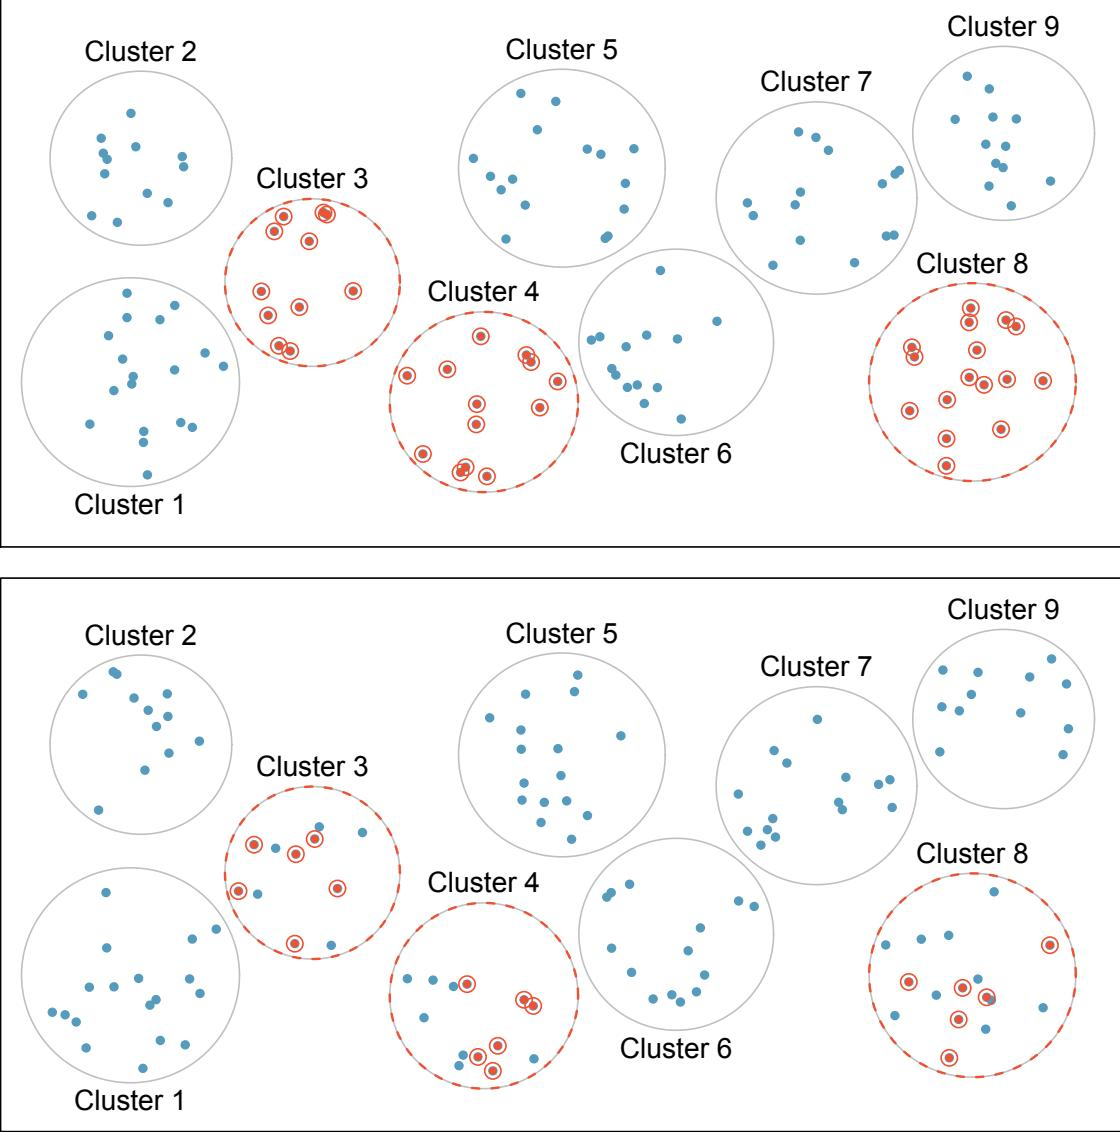
\includegraphics{_page_27_Figure_1.jpeg}

Figura 1.15: Ejemplos de muestreo por conglomerados y multietápico. En
el panel superior, se utilizó el muestreo por conglomerados: los datos
se agruparon en nueve conglomerados, se muestrearon tres de estos
conglomerados y se incluyeron todas las observaciones dentro de estos
tres conglomerados en la muestra. En el panel inferior, se utilizó el
muestreo multietápico, que difiere del muestreo por conglomerados solo
en que seleccionamos aleatoriamente un subconjunto de cada conglomerado
para incluirlo en la muestra en lugar de medir cada caso en cada
conglomerado muestreado.

\section{\texorpdfstring{\textbf{1.4.1 Principios del diseño
experimental}}{1.4.1 Principios del diseño experimental}}\label{principios-del-diseuxf1o-experimental}

Los experimentos aleatorizados generalmente se basan en cuatro
principios.

\begin{itemize}
\tightlist
\item
  Control. Los investigadores asignan tratamientos a los casos y hacen
  todo lo posible para controlar cualquier otra diferencia en los
  grupos.\hyperref[page-31-1]{27} Por ejemplo, cuando los pacientes
  toman un medicamento en forma de píldora, algunos pacientes toman la
  píldora con solo un sorbo de agua, mientras que otros pueden tomarla
  con un vaso entero de agua. Para controlar el efecto del consumo de
  agua, un médico puede pedir a todos los pacientes que beban un vaso de
  12 onzas de agua con la píldora.
\item
  Aleatorización. Los investigadores aleatorizan a los pacientes en
  grupos de tratamiento para tener en cuenta las variables que no se
  pueden controlar. Por ejemplo, algunos pacientes pueden ser más
  susceptibles a una enfermedad que otros debido a sus hábitos
  alimenticios. La aleatorización de los pacientes en el grupo de
  tratamiento o control ayuda a igualar tales diferencias y también
  evita que sesgos accidentales entren en el estudio.
\item
  Réplica. Cuantos más casos observen los investigadores, con mayor
  precisión podrán estimar el efecto de la variable explicativa sobre la
  respuesta. En un solo estudio, replicamos recogiendo una muestra
  suficientemente grande. Además, un grupo de científicos puede replicar
  un estudio completo para verificar un hallazgo anterior.
\item
  Bloqueo. Los investigadores a veces saben o sospechan que variables,
  además del tratamiento, influyen en la respuesta. En estas
  circunstancias, primero pueden agrupar a los individuos en función de
  esta variable en bloques y luego aleatorizar los casos dentro de cada
  bloque a los grupos de tratamiento. Esta estrategia se conoce a menudo
  como bloqueo. Por ejemplo, si estamos observando el efecto de un
  fármaco en los ataques cardíacos, podríamos primero dividir a los
  pacientes en el estudio en bloques de bajo riesgo y alto riesgo, luego
  asignar aleatoriamente la mitad de los pacientes de cada bloque al
  grupo de control y la otra mitad al grupo de tratamiento, como se
  muestra en la Figura \hyperref[page-32-0]{1.16.} Esta estrategia
  asegura que cada grupo de tratamiento tenga un número igual de
  pacientes de bajo riesgo y alto riesgo.
\end{itemize}

Es importante incorporar los tres primeros principios del diseño
experimental en cualquier estudio, y este libro describe los métodos
aplicables para analizar los datos de tales experimentos. El bloqueo es
una técnica un poco más avanzada, y los métodos estadísticos de este
libro pueden extenderse para analizar los datos recogidos mediante el
bloqueo.

\section{\texorpdfstring{\textbf{1.4.2 Reducción del sesgo en
experimentos con
humanos}}{1.4.2 Reducción del sesgo en experimentos con humanos}}\label{reducciuxf3n-del-sesgo-en-experimentos-con-humanos}

Los experimentos aleatorizados son el estándar de oro para la recogida
de datos, pero no garantizan una perspectiva imparcial sobre la relación
causa y efecto en todos los casos. Los estudios en humanos son ejemplos
perfectos donde el sesgo puede surgir sin querer. Aquí reconsideramos un
estudio donde se utilizó un nuevo fármaco para tratar a pacientes con
ataques cardíacos. En particular, los investigadores querían saber si el
fármaco reducía las muertes en los pacientes.

Estos investigadores diseñaron un experimento aleatorizado porque
querían sacar conclusiones causales sobre el efecto del fármaco. Los
voluntarios del estudio\hyperref[page-31-2]{28} fueron colocados
aleatoriamente en dos grupos de estudio. Un grupo, el grupo de
tratamiento, recibió el fármaco. El otro grupo, llamado grupo de
control, no recibió ningún tratamiento farmacológico.

27Este es un concepto diferente al de un grupo de control, que
discutimos en el segundo principio y en la Sección
\hyperref[page-31-3]{1.4.2.} 28Los sujetos humanos a menudo se llaman
pacientes, voluntarios o participantes del estudio.

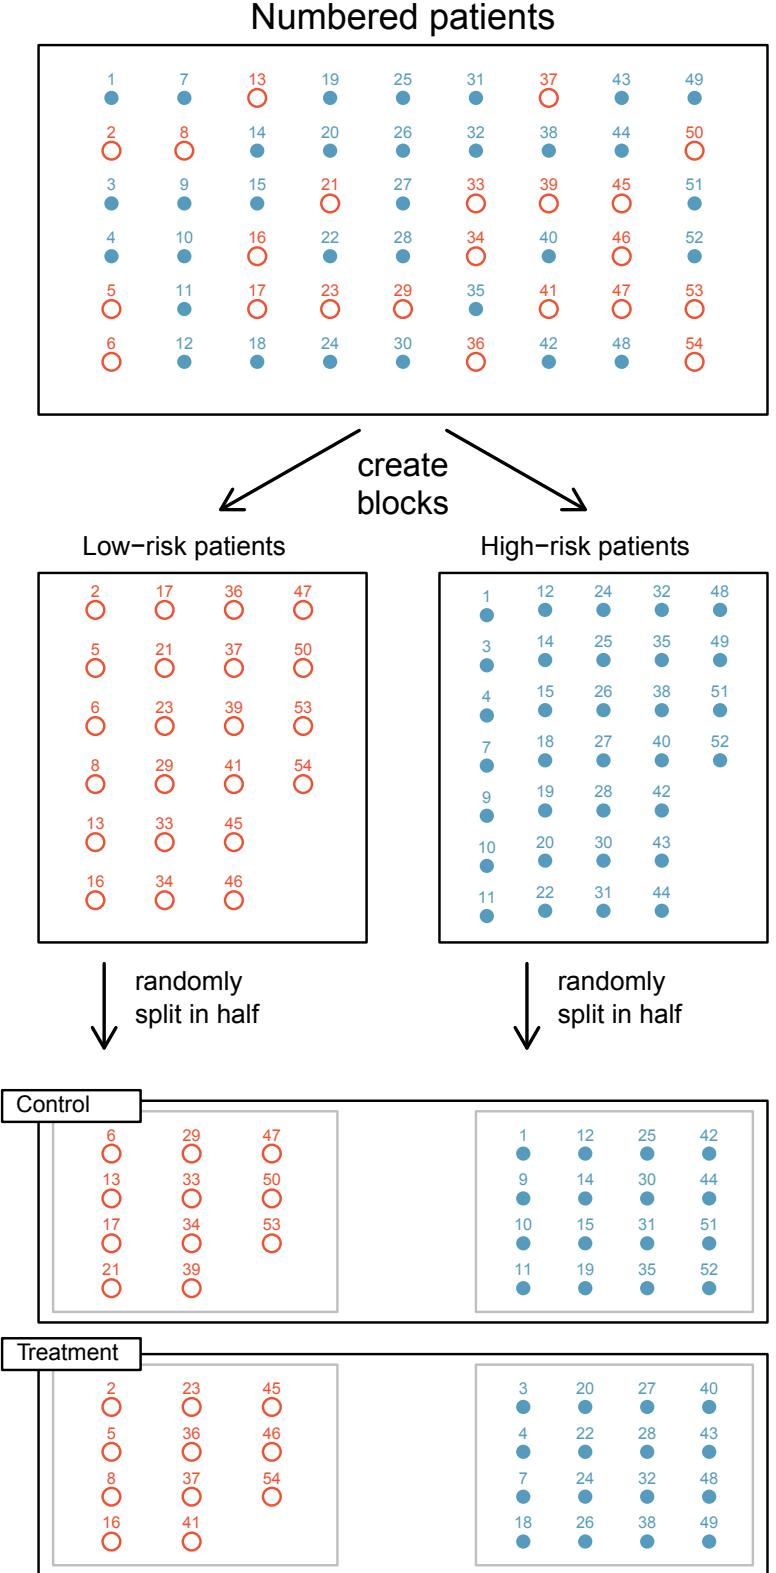
\includegraphics{_page_32_Figure_1.jpeg}

Figura 1.16: Bloqueo usando una variable que representa el riesgo del
paciente. Los pacientes se dividen primero en bloques de bajo riesgo y
alto riesgo, luego cada bloque se separa uniformemente en los grupos de
tratamiento utilizando la aleatorización. Esta estrategia asegura una
representación igual de pacientes en cada grupo de tratamiento tanto de
las categorías de bajo riesgo como de alto riesgo.

Ponte en el lugar de una persona en el estudio. Si estás en el grupo de
tratamiento, te dan un nuevo fármaco elegante que esperas que te ayude.
Por otro lado, una persona en el otro grupo no recibe el fármaco y se
sienta ociosamente, esperando que su participación no aumente su riesgo
de muerte. Estas perspectivas sugieren que en realidad hay dos efectos:
el de interés es la efectividad del fármaco, y el segundo es un efecto
emocional que es difícil de cuantificar.

Los investigadores no suelen estar interesados en el efecto emocional,
que podría sesgar el estudio. Para evitar este problema, los
investigadores no quieren que los pacientes sepan en qué grupo están.
Cuando los investigadores mantienen a los pacientes desinformados sobre
su tratamiento, se dice que el estudio es ciego. Pero hay un problema:
si un paciente no recibe un tratamiento, sabrá que está en el grupo de
control. La solución a este problema es dar tratamientos falsos a los
pacientes en el grupo de control. Un tratamiento falso se llama placebo,
y un placebo efectivo es la clave para hacer un estudio verdaderamente
ciego. Un ejemplo clásico de un placebo es una píldora de azúcar que
está hecha para parecerse a la píldora de tratamiento real. A menudo, un
placebo resulta en una mejora leve pero real en los pacientes. Este
efecto se ha denominado el efecto placebo.

Los pacientes no son los únicos que deben estar cegados: los médicos e
investigadores pueden sesgar accidentalmente un estudio. Cuando un
médico sabe que a un paciente se le ha dado el tratamiento real, podría
inadvertidamente darle a ese paciente más atención o cuidado que a un
paciente que sabe que está tomando el placebo. Para protegerse contra
este sesgo, que de nuevo se ha encontrado que tiene un efecto medible en
algunos casos, la mayoría de los estudios modernos emplean una
configuración doble ciego donde los médicos o investigadores que
interactúan con los pacientes son, al igual que los pacientes,
desconocedores de quién está o no recibiendo el
tratamiento.\hyperref[page-33-0]{29}

\paragraph{\texorpdfstring{\textbf{PRÁCTICA GUIADA
1.16}}{PRÁCTICA GUIADA 1.16}}\label{pruxe1ctica-guiada-1.16}

Vuelve al estudio de la Sección \hyperref[page-8-0]{1.1} donde los
investigadores estaban probando si los stents eran eficaces para reducir
los accidentes cerebrovasculares en pacientes de riesgo. ¿Es esto un
experimento? ¿Estaba cegado el estudio? ¿Fue doble
ciego?\hyperref[page-33-1]{30}

\paragraph{\texorpdfstring{\textbf{PRÁCTICA GUIADA
1.17}}{PRÁCTICA GUIADA 1.17}}\label{pruxe1ctica-guiada-1.17}

Para el estudio de la Sección \hyperref[page-8-0]{1.1,} ¿podrían los
investigadores haber empleado un placebo? Si es así, ¿cómo habría sido
ese placebo?\hyperref[page-33-2]{31}

Es posible que tengas muchas preguntas sobre la ética de las cirugías
simuladas para crear un placebo después de leer la Práctica Guiada
\hyperref[page-33-3]{1.17.} Estas preguntas pueden incluso haber surgido
en tu mente cuando en el contexto general del experimento, donde un
tratamiento posiblemente útil fue retenido de los individuos en el grupo
de control; la principal diferencia es que una cirugía simulada tiende a
crear un riesgo adicional, mientras que la retención de un tratamiento
sólo mantiene el riesgo de una persona.

Siempre hay múltiples puntos de vista de los experimentos y placebos, y
rara vez es obvio cuál es éticamente ``correcto''. Por ejemplo, ¿es
ético usar una cirugía simulada cuando crea un riesgo para el paciente?
Sin embargo, si no usamos cirugías simuladas, podemos promover el uso de
un tratamiento costoso que no tiene ningún efecto real; si esto sucede,
el dinero y otros recursos se desviarán de otros tratamientos que se
sabe que son útiles. En última instancia, esta es una situación difícil
donde no podemos proteger perfectamente tanto a los pacientes que se han
ofrecido voluntariamente para el estudio como a los pacientes que pueden
beneficiarse (o no) del tratamiento en el futuro.

29Siempre hay algunos investigadores involucrados en el estudio que sí
saben qué pacientes están recibiendo qué tratamiento. Sin embargo, no
interactúan con los pacientes del estudio y no les dicen a los
profesionales de la salud cegados quién está recibiendo qué tratamiento.

30Los investigadores asignaron a los pacientes a sus grupos de
tratamiento, por lo que este estudio fue un experimento. Sin embargo,
los pacientes podían distinguir qué tratamiento recibieron, por lo que
este estudio no fue ciego. El estudio no pudo ser doble ciego ya que no
fue ciego.

31En última instancia, ¿podemos hacer que los pacientes piensen que
fueron tratados por una cirugía? De hecho, podemos, y algunos
experimentos utilizan lo que se llama una cirugía simulada. En una
cirugía simulada, el paciente sí se somete a una cirugía, pero el
paciente no recibe el tratamiento completo, aunque todavía obtendrá un
efecto placebo.

\section{\texorpdfstring{\textbf{Ejercicios}}{Ejercicios}}\label{ejercicios-1}

\hyperref[page-384-4]{\textbf{1.29}} \textbf{Luz y rendimiento en
exámenes.} Se diseña un estudio para probar el efecto del nivel de luz
en el rendimiento en exámenes de los estudiantes. El investigador cree
que los niveles de luz podrían tener diferentes efectos en hombres y
mujeres, por lo que quiere asegurarse de que ambos estén representados
por igual en cada tratamiento. Los tratamientos son iluminación
fluorescente cenital, iluminación amarilla cenital y sin iluminación
cenital (solo lámparas de escritorio).

\begin{itemize}
\tightlist
\item
  \begin{enumerate}
  \def\labelenumi{(\alph{enumi})}
  \tightlist
  \item
    ¿Cuál es la variable de respuesta?
  \end{enumerate}
\item
  \begin{enumerate}
  \def\labelenumi{(\alph{enumi})}
  \setcounter{enumi}{1}
  \tightlist
  \item
    ¿Cuál es la variable explicativa? ¿Cuáles son sus niveles?
  \end{enumerate}
\item
  \begin{enumerate}
  \def\labelenumi{(\alph{enumi})}
  \setcounter{enumi}{2}
  \tightlist
  \item
    ¿Cuál es la variable de bloqueo? ¿Cuáles son sus niveles?
  \end{enumerate}
\end{itemize}

\hyperref[page-384-5]{\textbf{1.30}} \textbf{Suplementos vitamínicos.}
Para evaluar la eficacia de tomar grandes dosis de vitamina C para
reducir la duración del resfriado común, los investigadores reclutaron a
400 voluntarios sanos entre el personal y los estudiantes de una
universidad. A una cuarta parte de los pacientes se les asignó un
placebo, y el resto se dividió equitativamente entre 1 g de vitamina C,
3 g de vitamina C o 3 g de vitamina C más aditivos para tomar al inicio
de un resfriado durante los dos días siguientes. Todas las pastillas
tenían una apariencia y un embalaje idénticos. Las enfermeras que
entregaron las píldoras recetadas a los pacientes sabían qué paciente
recibió qué tratamiento, pero los investigadores que evaluaron a los
pacientes cuando estaban enfermos no lo sabían. No se observaron
diferencias significativas en ninguna medida de la duración o gravedad
del resfriado entre los cuatro grupos, y el grupo placebo tuvo la
duración más corta de los síntomas.\hyperref[page-34-0]{32}

\begin{itemize}
\tightlist
\item
  \begin{enumerate}
  \def\labelenumi{(\alph{enumi})}
  \tightlist
  \item
    ¿Fue esto un experimento o un estudio observacional? ¿Por qué?
  \end{enumerate}
\item
  \begin{enumerate}
  \def\labelenumi{(\alph{enumi})}
  \setcounter{enumi}{1}
  \tightlist
  \item
    ¿Cuáles son las variables explicativas y de respuesta en este
    estudio?
  \end{enumerate}
\item
  \begin{enumerate}
  \def\labelenumi{(\alph{enumi})}
  \setcounter{enumi}{2}
  \tightlist
  \item
    ¿Se cegó a los pacientes a su tratamiento?
  \end{enumerate}
\item
  \begin{enumerate}
  \def\labelenumi{(\alph{enumi})}
  \setcounter{enumi}{3}
  \tightlist
  \item
    ¿Fue este estudio doble ciego?
  \end{enumerate}
\item
  \begin{enumerate}
  \def\labelenumi{(\alph{enumi})}
  \setcounter{enumi}{4}
  \tightlist
  \item
    En última instancia, los participantes pueden elegir si usar o no
    las píldoras que se les recetaron. Podríamos esperar que no todos se
    adhieran y tomen sus píldoras. ¿Introduce esto una variable de
    confusión en el estudio? Explica tu razonamiento.
  \end{enumerate}
\end{itemize}

\hyperref[page-384-6]{\textbf{1.31}} \textbf{Luz, ruido y rendimiento en
exámenes.} Se diseña un estudio para probar el efecto del nivel de luz y
el nivel de ruido en el rendimiento en exámenes de los estudiantes. El
investigador cree que los niveles de luz y ruido podrían tener
diferentes efectos en hombres y mujeres, por lo que quiere asegurarse de
que ambos estén representados por igual en cada tratamiento. Los
tratamientos de luz considerados son iluminación fluorescente cenital,
iluminación amarilla cenital y sin iluminación cenital (solo lámparas de
escritorio). Los tratamientos de ruido considerados son sin ruido, ruido
de construcción y ruido de conversación humana.

\begin{itemize}
\tightlist
\item
  \begin{enumerate}
  \def\labelenumi{(\alph{enumi})}
  \tightlist
  \item
    ¿Qué tipo de estudio es este?
  \end{enumerate}
\item
  \begin{enumerate}
  \def\labelenumi{(\alph{enumi})}
  \setcounter{enumi}{1}
  \tightlist
  \item
    ¿Cuántos factores se consideran en este estudio? Identifíquelos y
    describa sus niveles.
  \end{enumerate}
\item
  \begin{enumerate}
  \def\labelenumi{(\alph{enumi})}
  \setcounter{enumi}{2}
  \tightlist
  \item
    ¿Cuál es el papel de la variable sexo en este estudio?
  \end{enumerate}
\end{itemize}

\hyperref[page-384-7]{\textbf{1.32}} \textbf{Música y aprendizaje.} Le
gustaría realizar un experimento en clase para ver si los estudiantes
aprenden mejor si estudian sin música, con música sin letra
(instrumental) o con música con letra. Describa brevemente un diseño
para este estudio.

\hyperref[page-384-8]{\textbf{1.33}} \textbf{Preferencia por los
refrescos.} Le gustaría realizar un experimento en clase para ver si sus
compañeros de clase prefieren el sabor de la Coca-Cola normal o la
Coca-Cola Light. Describa brevemente un diseño para este estudio.

\hyperref[page-384-9]{\textbf{1.34}} \textbf{Ejercicio y salud mental.}
Un investigador está interesado en los efectos del ejercicio en la salud
mental y propone el siguiente estudio: Utilizar un muestreo aleatorio
estratificado para asegurar proporciones representativas de personas de
18-30, 31-40 y 41-55 años de la población. A continuación, asignar
aleatoriamente a la mitad de los sujetos de cada grupo de edad a hacer
ejercicio dos veces por semana, e instruir al resto para que no hagan
ejercicio. Realizar un examen de salud mental al principio y al final
del estudio, y comparar los resultados.

\begin{itemize}
\tightlist
\item
  \begin{enumerate}
  \def\labelenumi{(\alph{enumi})}
  \tightlist
  \item
    ¿Qué tipo de estudio es este?
  \end{enumerate}
\item
  \begin{enumerate}
  \def\labelenumi{(\alph{enumi})}
  \setcounter{enumi}{1}
  \tightlist
  \item
    ¿Cuáles son los grupos de tratamiento y control en este estudio?
  \end{enumerate}
\item
  \begin{enumerate}
  \def\labelenumi{(\alph{enumi})}
  \setcounter{enumi}{2}
  \tightlist
  \item
    ¿Este estudio utiliza el bloqueo? Si es así, ¿cuál es la variable de
    bloqueo?
  \end{enumerate}
\item
  \begin{enumerate}
  \def\labelenumi{(\alph{enumi})}
  \setcounter{enumi}{3}
  \tightlist
  \item
    ¿Este estudio utiliza el cegamiento?
  \end{enumerate}
\item
  \begin{enumerate}
  \def\labelenumi{(\alph{enumi})}
  \setcounter{enumi}{4}
  \tightlist
  \item
    Comente si los resultados del estudio pueden utilizarse para
    establecer una relación causal entre el ejercicio y la salud mental,
    e indique si las conclusiones pueden generalizarse a la población en
    general.
  \end{enumerate}
\item
  \begin{enumerate}
  \def\labelenumi{(\alph{enumi})}
  \setcounter{enumi}{5}
  \tightlist
  \item
    Supongamos que se le encarga la tarea de determinar si este estudio
    propuesto debe recibir financiación. ¿Tendría alguna reserva sobre
    la propuesta de estudio?
  \end{enumerate}
\end{itemize}

32C. Audera et
al.~\href{http://www.openintro.org/redirect.php?go=textbook-vitamin_C_cold_treatment_2001&referrer=os4_pdf}{``Mega-dose
vitamin C in treatment of the common cold: a randomised controlled
trial''}. En: Medical Journal of Australia 175.7 (2001), pp.~359--362.

\section{\texorpdfstring{\textbf{Ejercicios del
Capítulo}}{Ejercicios del Capítulo}}\label{ejercicios-del-capuxedtulo}

\hyperref[page-384-10]{\textbf{1.35}} \textbf{Nombres de mascotas.} La
ciudad de Seattle, WA tiene un portal de datos abiertos que incluye
mascotas registradas en la ciudad. Para cada mascota registrada, tenemos
información sobre el nombre y la especie de la mascota. La siguiente
visualización grafica la proporción de perros con un nombre dado versus
la proporción de gatos con el mismo nombre. Se muestran los 20 nombres
de gatos y perros más comunes. La línea diagonal en el gráfico es la
línea x = y; si un nombre apareciera en esta línea, la popularidad del
nombre sería exactamente la misma para perros y gatos.

\begin{itemize}
\tightlist
\item
  \begin{enumerate}
  \def\labelenumi{(\alph{enumi})}
  \tightlist
  \item
    ¿Estos datos se recopilaron como parte de un experimento o de un
    estudio observacional?
  \end{enumerate}
\item
  \begin{enumerate}
  \def\labelenumi{(\alph{enumi})}
  \setcounter{enumi}{1}
  \tightlist
  \item
    ¿Cuál es el nombre de perro más común? ¿Cuál es el nombre de gato
    más común?
  \end{enumerate}
\item
  \begin{enumerate}
  \def\labelenumi{(\alph{enumi})}
  \setcounter{enumi}{2}
  \tightlist
  \item
    ¿Qué nombres son más comunes para gatos que para perros?
  \end{enumerate}
\item
  \begin{enumerate}
  \def\labelenumi{(\alph{enumi})}
  \setcounter{enumi}{3}
  \tightlist
  \item
    ¿La relación entre las dos variables es positiva o negativa? ¿Qué
    significa esto en el contexto de los datos?
  \end{enumerate}
\end{itemize}

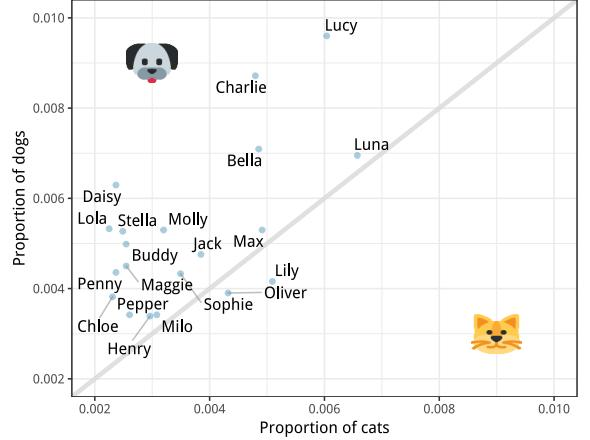
\includegraphics{_page_35_Figure_7.jpeg}

\hyperref[page-384-11]{\textbf{1.36}} \textbf{Estresado, Parte II.} En
un estudio que evalúa la relación entre el estrés y los calambres
musculares, la mitad de los sujetos son asignados aleatoriamente a ser
expuestos a un aumento del estrés al ser colocados en un ascensor que
cae rápidamente y se detiene abruptamente y la otra mitad se deja sin
estrés o con estrés basal.

\begin{itemize}
\tightlist
\item
  \begin{enumerate}
  \def\labelenumi{(\alph{enumi})}
  \tightlist
  \item
    ¿Qué tipo de estudio es este?
  \end{enumerate}
\item
  \begin{enumerate}
  \def\labelenumi{(\alph{enumi})}
  \setcounter{enumi}{1}
  \tightlist
  \item
    ¿Se puede utilizar este estudio para concluir una relación causal
    entre el aumento del estrés y los calambres musculares?
  \end{enumerate}
\end{itemize}

\hyperref[page-384-12]{\textbf{1.37}} \textbf{Semillas de chía y pérdida
de peso.} Chia Pets -- esas figuritas de terracota a las que les brota
un cabello verde y difuso -- hicieron de la planta de chía un nombre
familiar. Pero la chía ha ganado una reputación completamente nueva como
suplemento dietético. En un estudio de 2009, un equipo de investigadores
reclutó a 38 hombres y los dividió aleatoriamente en dos grupos:
tratamiento o control. También reclutaron a 38 mujeres y asignaron
aleatoriamente a la mitad de estas participantes al grupo de tratamiento
y a la otra mitad al grupo de control. Un grupo recibió 25 gramos de
semillas de chía dos veces al día y el otro recibió un placebo. Los
sujetos se ofrecieron voluntariamente a participar en el estudio.
Después de 12 semanas, los científicos no encontraron diferencias
significativas entre los grupos en el apetito o la pérdida de
peso.\hyperref[page-35-0]{33}

\begin{itemize}
\tightlist
\item
  \begin{enumerate}
  \def\labelenumi{(\alph{enumi})}
  \tightlist
  \item
    ¿Qué tipo de estudio es este?
  \end{enumerate}
\item
  \begin{enumerate}
  \def\labelenumi{(\alph{enumi})}
  \setcounter{enumi}{1}
  \tightlist
  \item
    ¿Cuáles son los tratamientos experimentales y de control en este
    estudio?
  \end{enumerate}
\item
  \begin{enumerate}
  \def\labelenumi{(\alph{enumi})}
  \setcounter{enumi}{2}
  \tightlist
  \item
    ¿Se ha utilizado el bloqueo en este estudio? Si es así, ¿cuál es la
    variable de bloqueo?
  \end{enumerate}
\item
  \begin{enumerate}
  \def\labelenumi{(\alph{enumi})}
  \setcounter{enumi}{3}
  \tightlist
  \item
    ¿Se ha utilizado el cegamiento en este estudio?
  \end{enumerate}
\item
  \begin{enumerate}
  \def\labelenumi{(\alph{enumi})}
  \setcounter{enumi}{4}
  \tightlist
  \item
    Comente si podemos o no hacer una declaración causal e indique si
    podemos o no generalizar la conclusión a la población en general.
  \end{enumerate}
\end{itemize}

\hyperref[page-384-13]{\textbf{1.38}} \textbf{Encuesta del consejo
municipal.} Un consejo municipal ha solicitado que se realice una
encuesta de hogares en una zona suburbana de su ciudad. La zona se
divide en muchos barrios distintos y únicos, algunos con casas grandes,
otros solo con apartamentos y otros con una mezcla diversa de
estructuras de vivienda. Para cada parte a continuación, identifique los
métodos de muestreo descritos y describa los pros y los contras
estadísticos del método en el contexto de la ciudad.

\begin{itemize}
\tightlist
\item
  \begin{enumerate}
  \def\labelenumi{(\alph{enumi})}
  \tightlist
  \item
    Muestrear aleatoriamente 200 hogares de la ciudad.
  \end{enumerate}
\item
  \begin{enumerate}
  \def\labelenumi{(\alph{enumi})}
  \setcounter{enumi}{1}
  \tightlist
  \item
    Dividir la ciudad en 20 barrios y muestrear 10 hogares de cada
    barrio.
  \end{enumerate}
\item
  \begin{enumerate}
  \def\labelenumi{(\alph{enumi})}
  \setcounter{enumi}{2}
  \tightlist
  \item
    Dividir la ciudad en 20 barrios, muestrear aleatoriamente 3 barrios
    y luego muestrear todos los hogares de esos 3 barrios.
  \end{enumerate}
\item
  \begin{enumerate}
  \def\labelenumi{(\alph{enumi})}
  \setcounter{enumi}{3}
  \tightlist
  \item
    Dividir la ciudad en 20 barrios, muestrear aleatoriamente 8 barrios
    y luego muestrear aleatoriamente 50 hogares de esos barrios.
  \end{enumerate}
\item
  \begin{enumerate}
  \def\labelenumi{(\alph{enumi})}
  \setcounter{enumi}{4}
  \tightlist
  \item
    Muestrear los 200 hogares más cercanos a las oficinas del consejo
    municipal.
  \end{enumerate}
\end{itemize}

33D.C. Nieman et
al.~\href{http://www.openintro.org/redirect.php?go=textbook-chia_seeds_2009&referrer=os4_pdf}{``La
semilla de chía no promueve la pérdida de peso ni altera los factores de
riesgo de enfermedad en adultos con sobrepeso''}. En: Nutrition Research
29.6 (2009), pp.~414--418.

\section{1.4. EXPERIMENTOS 37}\label{experimentos-37}

\hyperref[page-384-14]{\textbf{1.39}} \textbf{Razonamiento defectuoso.}
Identifique la(s) falla(s) en el razonamiento en los siguientes
escenarios. Explique qué deberían haber hecho de manera diferente los
individuos en el estudio si querían sacar conclusiones tan fuertes.

\begin{itemize}
\tightlist
\item
  \begin{enumerate}
  \def\labelenumi{(\alph{enumi})}
  \tightlist
  \item
    A los estudiantes de una escuela primaria se les entrega un
    cuestionario que se les pide que devuelvan después de que sus padres
    lo hayan completado. Una de las preguntas formuladas es:
    ``¿Considera que su horario de trabajo le dificulta pasar tiempo con
    sus hijos después de la escuela?'' De los padres que respondieron,
    el 85\% dijo ``no''. Con base en estos resultados, los funcionarios
    de la escuela concluyen que una gran mayoría de los padres no tienen
    dificultad para pasar tiempo con sus hijos después de la escuela.
  \end{enumerate}
\item
  \begin{enumerate}
  \def\labelenumi{(\alph{enumi})}
  \setcounter{enumi}{1}
  \tightlist
  \item
    Se realiza una encuesta en una muestra aleatoria simple de 1,000
    mujeres que recientemente dieron a luz, preguntándoles si fumaron o
    no durante el embarazo. Una encuesta de seguimiento que pregunta si
    los niños tienen problemas respiratorios se lleva a cabo 3 años
    después. Sin embargo, solo se localiza a 567 de estas mujeres en la
    misma dirección. El investigador informa que estas 567 mujeres son
    representativas de todas las madres.
  \end{enumerate}
\item
  \begin{enumerate}
  \def\labelenumi{(\alph{enumi})}
  \setcounter{enumi}{2}
  \tightlist
  \item
    Un ortopedista administra un cuestionario a 30 de sus pacientes que
    no tienen ningún problema articular y encuentra que 20 de ellos
    corren con regularidad. Concluye que correr disminuye el riesgo de
    problemas articulares.
  \end{enumerate}
\end{itemize}

\hyperref[page-384-15]{\textbf{1.40}} \textbf{Ingresos y educación en
los condados de EE. UU.} El diagrama de dispersión a continuación
muestra la relación entre el ingreso per cápita (en miles de dólares) y
el porcentaje de población con una licenciatura en 3,143 condados en los
EE. UU. en 2010.

\begin{itemize}
\tightlist
\item
  \begin{enumerate}
  \def\labelenumi{(\alph{enumi})}
  \tightlist
  \item
    ¿Cuáles son las variables explicativa y de respuesta?
  \end{enumerate}
\item
  \begin{enumerate}
  \def\labelenumi{(\alph{enumi})}
  \setcounter{enumi}{1}
  \tightlist
  \item
    Describe la relación entre las dos variables. Asegúrese de discutir
    las observaciones inusuales, si las hay.
  \end{enumerate}
\item
  \begin{enumerate}
  \def\labelenumi{(\alph{enumi})}
  \setcounter{enumi}{2}
  \tightlist
  \item
    ¿Podemos concluir que tener una licenciatura aumenta los ingresos de
    uno?
  \end{enumerate}
\end{itemize}

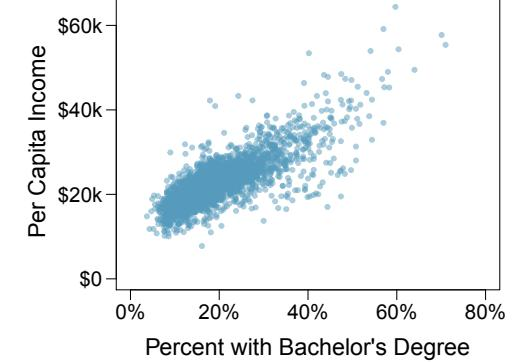
\includegraphics{_page_36_Figure_9.jpeg}

\hyperref[page-384-16]{\textbf{1.41}} \textbf{¿Comer mejor, sentirse
mejor?} En un estudio de salud pública sobre los efectos del consumo de
frutas y verduras en el bienestar psicológico en adultos jóvenes, los
participantes fueron asignados aleatoriamente a tres grupos: (1) dietas
habituales, (2) una intervención ecológica momentánea que involucraba
recordatorios por mensaje de texto para aumentar su consumo de frutas y
verduras más un vale para comprarlas, o (3) una intervención de frutas y
verduras en la que se les daba a los participantes dos porciones diarias
adicionales de frutas y verduras frescas para consumir además de su
dieta normal. Se les pidió a los participantes que realizaran una
encuesta nocturna en sus teléfonos inteligentes. Los participantes
fueron estudiantes voluntarios de la Universidad de Otago, Nueva
Zelanda. Al final del estudio de 14 días, solo los participantes en el
tercer grupo mostraron mejoras en su bienestar psicológico durante los
14 días en relación con los otros grupos.\hyperref[page-36-0]{34}

\begin{itemize}
\tightlist
\item
  \begin{enumerate}
  \def\labelenumi{(\alph{enumi})}
  \tightlist
  \item
    ¿Qué tipo de estudio es este?
  \end{enumerate}
\item
  \begin{enumerate}
  \def\labelenumi{(\alph{enumi})}
  \setcounter{enumi}{1}
  \tightlist
  \item
    Identifique las variables explicativas y de respuesta.
  \end{enumerate}
\item
  \begin{enumerate}
  \def\labelenumi{(\alph{enumi})}
  \setcounter{enumi}{2}
  \tightlist
  \item
    Comente si los resultados del estudio se pueden generalizar a la
    población.
  \end{enumerate}
\item
  \begin{enumerate}
  \def\labelenumi{(\alph{enumi})}
  \setcounter{enumi}{3}
  \tightlist
  \item
    Comente si los resultados del estudio se pueden utilizar para
    establecer relaciones causales.
  \end{enumerate}
\item
  (e) Un artículo periodístico que informa sobre el estudio afirma:
  ``Los resultados de este estudio demuestran que dar a los adultos
  jóvenes frutas y verduras frescas para comer puede tener beneficios
  psicológicos, incluso durante un breve período de tiempo''. ¿Cómo
  sugeriría revisar esta declaración para que pueda ser respaldada por
  el estudio?
\end{itemize}

\hyperref[page-384-17]{\textbf{1.42}} \textbf{Pantallas, adolescentes y
bienestar psicológico.} En un estudio de tres grandes conjuntos de datos
representativos a nivel nacional de Irlanda, Estados Unidos y el Reino
Unido (n = 17,247), se les pidió a los adolescentes entre las edades de
12 a 15 años que llevaran un diario de su tiempo frente a la pantalla y
respondieran preguntas sobre cómo se sentían o actuaban. Las respuestas
a estas preguntas se utilizaron luego para calcular una puntuación de
bienestar psicológico. Se recopilaron datos adicionales y se incluyeron
en el análisis, como el sexo y la edad de cada niño, y la educación, el
origen étnico, la angustia psicológica y el empleo de la madre. El
estudio concluyó que hay poca evidencia clara de que el tiempo frente a
la pantalla disminuya el bienestar de los
adolescentes.\hyperref[page-37-0]{35}

\begin{itemize}
\tightlist
\item
  \begin{enumerate}
  \def\labelenumi{(\alph{enumi})}
  \tightlist
  \item
    ¿Qué tipo de estudio es este?
  \end{enumerate}
\item
  \begin{enumerate}
  \def\labelenumi{(\alph{enumi})}
  \setcounter{enumi}{1}
  \tightlist
  \item
    Identifique las variables explicativas.
  \end{enumerate}
\item
  \begin{enumerate}
  \def\labelenumi{(\alph{enumi})}
  \setcounter{enumi}{2}
  \tightlist
  \item
    Identifique la variable de respuesta.
  \end{enumerate}
\item
  \begin{enumerate}
  \def\labelenumi{(\alph{enumi})}
  \setcounter{enumi}{3}
  \tightlist
  \item
    Comente si los resultados del estudio se pueden generalizar a la
    población y por qué.
  \end{enumerate}
\item
  \begin{enumerate}
  \def\labelenumi{(\alph{enumi})}
  \setcounter{enumi}{4}
  \tightlist
  \item
    Comente si los resultados del estudio se pueden utilizar para
    establecer relaciones causales.
  \end{enumerate}
\end{itemize}

\hyperref[page-384-18]{\textbf{1.43}} \textbf{Stanford Open Policing.}
El proyecto Stanford Open Policing recopila, analiza y publica registros
de paradas de tráfico por parte de las agencias de aplicación de la ley
en los Estados Unidos. Su objetivo es ayudar a los investigadores,
periodistas y formuladores de políticas a investigar y mejorar las
interacciones entre la policía y el público.\hyperref[page-37-1]{36} El
siguiente es un extracto de una tabla resumen creada a partir de los
datos recopilados como parte de este proyecto.

\begin{longtable}[]{@{}
  >{\raggedright\arraybackslash}p{(\columnwidth - 10\tabcolsep) * \real{0.1667}}
  >{\raggedright\arraybackslash}p{(\columnwidth - 10\tabcolsep) * \real{0.1667}}
  >{\raggedright\arraybackslash}p{(\columnwidth - 10\tabcolsep) * \real{0.1667}}
  >{\raggedright\arraybackslash}p{(\columnwidth - 10\tabcolsep) * \real{0.1667}}
  >{\raggedright\arraybackslash}p{(\columnwidth - 10\tabcolsep) * \real{0.1667}}
  >{\raggedright\arraybackslash}p{(\columnwidth - 10\tabcolsep) * \real{0.1667}}@{}}
\toprule\noalign{}
\begin{minipage}[b]{\linewidth}\raggedright
\end{minipage} & \begin{minipage}[b]{\linewidth}\raggedright
\end{minipage} & \begin{minipage}[b]{\linewidth}\raggedright
Raza del
\end{minipage} & \begin{minipage}[b]{\linewidth}\raggedright
No.~de paradas
\end{minipage} & \begin{minipage}[b]{\linewidth}\raggedright
\end{minipage} & \begin{minipage}[b]{\linewidth}\raggedright
\% de conductores
\end{minipage} \\
\midrule\noalign{}
\endhead
\bottomrule\noalign{}
\endlastfoot
Condado & Estado & conductor & por año & coches registrados &
arrestados \\
Apaice County & Arizona & Negra & 266 & 0.08 & 0.02 \\
Apaice County & Arizona & Hispana & 1008 & 0.05 & 0.02 \\
Apaice County & Arizona & Blanca & 6322 & 0.02 & 0.01 \\
Cochise County & Arizona & Negra & 1169 & 0.05 & 0.01 \\
Cochise County & Arizona & Hispana & 9453 & 0.04 & 0.01 \\
Cochise County & Arizona & Blanca & 10826 & 0.02 & 0.01 \\
· · · & · · · & · · · & · · · & · · · & · · · \\
Wood County & Wisconsin & Negra & 16 & 0.24 & 0.10 \\
Wood County & Wisconsin & Hispana & 27 & 0.04 & 0.03 \\
Wood County & Wisconsin & Blanca & 1157 & 0.03 & 0.03 \\
\end{longtable}

\begin{itemize}
\tightlist
\item
  \begin{enumerate}
  \def\labelenumi{(\alph{enumi})}
  \tightlist
  \item
    ¿Qué variables se recopilaron en cada parada de tráfico individual
    para crear la tabla resumen anterior?
  \end{enumerate}
\item
  \begin{enumerate}
  \def\labelenumi{(\alph{enumi})}
  \setcounter{enumi}{1}
  \tightlist
  \item
    Indique si cada variable es numérica o categórica. Si es numérica,
    indique si es continua o discreta. Si es categórica, indique si es
    ordinal o no.
  \end{enumerate}
\item
  \begin{enumerate}
  \def\labelenumi{(\alph{enumi})}
  \setcounter{enumi}{2}
  \tightlist
  \item
    Supongamos que queremos evaluar si las tasas de registro de
    vehículos son diferentes para los conductores de diferentes razas.
    En este análisis, ¿qué variable sería la variable de respuesta y qué
    variable sería la variable explicativa?
  \end{enumerate}
\end{itemize}

\hyperref[page-384-19]{\textbf{1.44}} \textbf{Lanzamientos espaciales.}
La siguiente tabla resumen muestra el número de lanzamientos espaciales
en los EE. UU. por el tipo de agencia de lanzamiento y el resultado del
lanzamiento (éxito o fracaso).\hyperref[page-37-2]{37}

\begin{longtable}[]{@{}lllll@{}}
\toprule\noalign{}
& & 1957 - 1999 & & 2000 - 2018 \\
\midrule\noalign{}
\endhead
\bottomrule\noalign{}
\endlastfoot
& Fracaso & Éxito & Fracaso & Éxito \\
Privada & 13 & 295 & 10 & 562 \\
Estatal & 281 & 3751 & 33 & 711 \\
Startup & - & - & 5 & 65 \\
\end{longtable}

\begin{itemize}
\tightlist
\item
  \begin{enumerate}
  \def\labelenumi{(\alph{enumi})}
  \tightlist
  \item
    ¿Qué variables se recopilaron en cada lanzamiento para crear la
    tabla resumen anterior?
  \end{enumerate}
\item
  \begin{enumerate}
  \def\labelenumi{(\alph{enumi})}
  \setcounter{enumi}{1}
  \tightlist
  \item
    Indique si cada variable es numérica o categórica. Si es numérica,
    indique si es continua o discreta. Si es categórica, indique si es
    ordinal o no.
  \end{enumerate}
\item
  \begin{enumerate}
  \def\labelenumi{(\alph{enumi})}
  \setcounter{enumi}{2}
  \tightlist
  \item
    Supongamos que queremos estudiar cómo varía la tasa de éxito de los
    lanzamientos entre las agencias de lanzamiento y con el tiempo. En
    este análisis, ¿qué variable sería la variable de respuesta y qué
    variable sería la variable explicativa?
  \end{enumerate}
\end{itemize}

37Base de datos de vehículos de lanzamiento JSR,
\href{http://www.openintro.org/redirect.php?go=textbook-space-launches-data&referrer=os4_pdf}{Una
lista completa de lanzamientos espaciales suborbitales, edición del 10
de febrero de 2019.}

35Amy Orben y AK Baukney-Przybylski.
\href{http://www.openintro.org/redirect.php?go=textbook-screens_orben_2018&referrer=os4_pdf}{``Pantallas,
adolescentes y bienestar psicológico: evidencia de tres}
\href{http://www.openintro.org/redirect.php?go=textbook-screens_orben_2018&referrer=os4_pdf}{estudios
de diario de uso del tiempo''}. En: Psychological Science (2018).

36Emma Pierson et
al.~\href{http://www.openintro.org/redirect.php?go=textbook-police_pierson_2017&referrer=os4_pdf}{``Un
análisis a gran escala de las disparidades raciales en las paradas
policiales en los Estados Unidos''}. En: arXiv preprint arXiv:1706.05678
(2017).

\section{\texorpdfstring{\textbf{Capítulo
2}}{Capítulo 2}}\label{capuxedtulo-2}

39

\section{\texorpdfstring{\textbf{Resumiendo
datos}}{Resumiendo datos}}\label{resumiendo-datos}

\begin{itemize}
\tightlist
\item
  \hyperref[page-40-0]{\textbf{2.1}}
  \hyperref[page-40-0]{\textbf{Examinando datos numéricos}}
\item
  \hyperref[page-60-0]{\textbf{2.2}}
  \hyperref[page-60-0]{\textbf{Considerando datos categóricos}}
\item
  \hyperref[page-70-0]{\textbf{2.3}}
  \hyperref[page-70-0]{\textbf{Estudio de caso: vacuna contra la
  malaria}}
\end{itemize}

Este capítulo se centra en la mecánica y la construcción de estadísticas
resumidas y gráficos. Utilizamos software estadístico para generar los
resúmenes y gráficos presentados en este capítulo y libro. Sin embargo,
dado que esta podría ser su primera exposición a estos conceptos, nos
tomamos nuestro tiempo en este capítulo para detallar cómo crearlos. El
dominio del contenido presentado en este capítulo será crucial para
comprender los métodos y técnicas introducidos en el resto del libro.


\includegraphics{_page_39_Picture_1.jpeg}

Para videos, diapositivas y otros recursos, visite
\href{http://www.openintro.org/redirect.php?go=os&referrer=os4_pdf}{www.openintro.org/os}

\section{\texorpdfstring{\textbf{2.1 Examinando datos
numéricos}}{2.1 Examinando datos numéricos}}\label{examinando-datos-numuxe9ricos}

En esta sección exploraremos técnicas para resumir variables numéricas.
Por ejemplo, considere la variable de monto del préstamo del conjunto de
datos loan50, que representa el tamaño del préstamo para los 50
préstamos en el conjunto de datos. Esta variable es numérica ya que
podemos discutir sensatamente la diferencia numérica del tamaño de dos
préstamos. Por otro lado, los códigos de área y los códigos postales no
son numéricos, sino que son variables categóricas.

A lo largo de esta sección y la siguiente, aplicaremos estos métodos
utilizando los conjuntos de datos loan50 y county, que se presentaron en
la Sección \hyperref[page-11-0]{1.2.} Si desea revisar las variables de
cualquiera de los conjuntos de datos, consulte las Figuras
\hyperref[page-11-1]{1.3} y \hyperref[page-13-0]{1.5.}

\section{\texorpdfstring{\textbf{2.1.1 Diagramas de Dispersión para
Datos
Pareados}}{2.1.1 Diagramas de Dispersión para Datos Pareados}}\label{diagramas-de-dispersiuxf3n-para-datos-pareados}

Un diagrama de dispersión proporciona una vista caso por caso de los
datos para dos variables numéricas. En la Figura
\hyperref[page-15-0]{1.8} en la página \hyperref[page-15-0]{16,} se
utilizó un diagrama de dispersión para examinar la tasa de propiedad de
vivienda en contra de la fracción de unidades de vivienda que formaban
parte de propiedades de unidades múltiples (por ejemplo, apartamentos)
en el conjunto de datos del condado. Otro diagrama de dispersión se
muestra en la Figura \hyperref[page-40-1]{2.1,} comparando el ingreso
total de un prestatario (ingreso total) y la cantidad que pidió prestada
(monto del préstamo) para el conjunto de datos loan50. En cualquier
diagrama de dispersión, cada punto representa un solo caso. Dado que hay
50 casos en loan50, hay 50 puntos en la Figura
\hyperref[page-40-1]{2.1.}

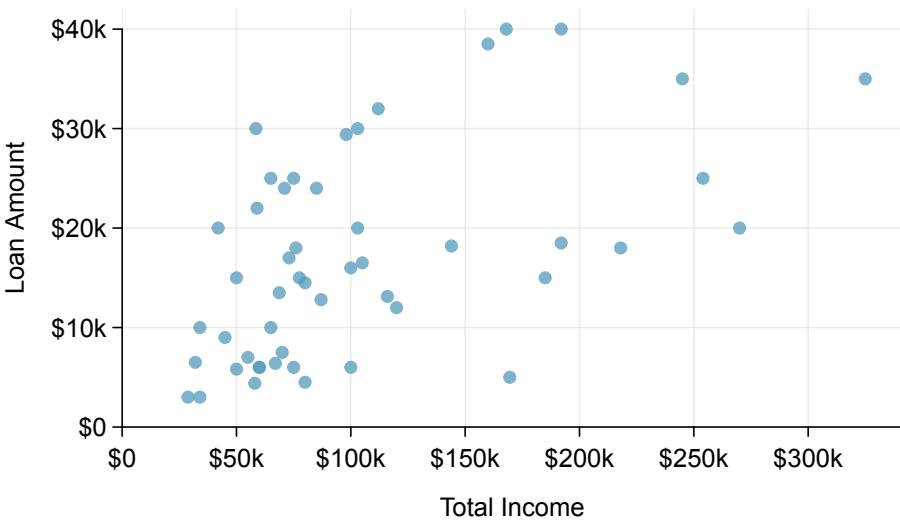
\includegraphics{_page_40_Figure_6.jpeg}

Figura 2.1: Un diagrama de dispersión del ingreso total versus el monto
del préstamo para el conjunto de datos loan50.

Mirando la Figura \hyperref[page-40-1]{2.1,} vemos que hay muchos
prestatarios con un ingreso por debajo de \$100,000 en el lado izquierdo
del gráfico, mientras que hay un puñado de prestatarios con ingresos
superiores a \$250,000.

\section{\texorpdfstring{\textbf{EJEMPLO
2.1}}{EJEMPLO 2.1}}\label{ejemplo-2.1}

La Figura \hyperref[page-41-0]{2.2} muestra un gráfico del ingreso
familiar mediano contra la tasa de pobreza para 3,142 condados. ¿Qué se
puede decir sobre la relación entre estas variables?

La relación es evidentemente no lineal, como se destaca con la línea
discontinua. Esto es diferente de los diagramas de dispersión anteriores
que hemos visto, que muestran relaciones que no muestran mucha, si es
que alguna, curvatura en la tendencia.

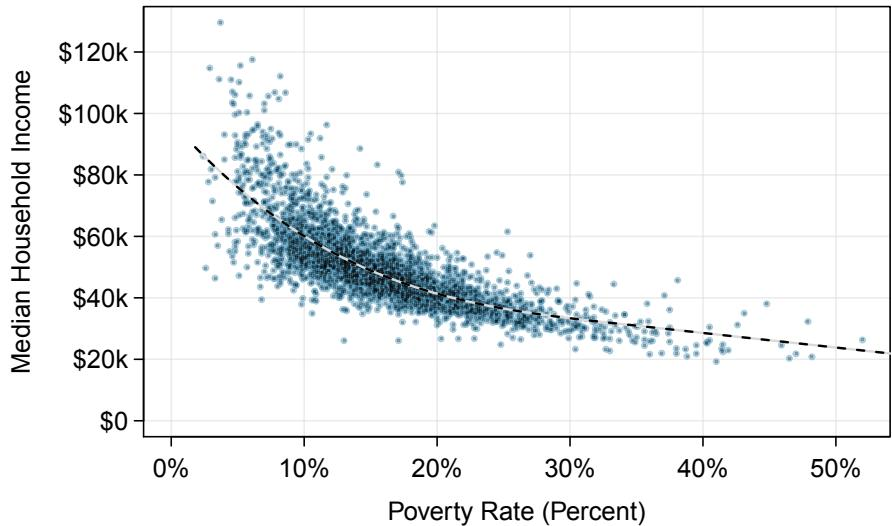
\includegraphics{_page_41_Figure_1.jpeg}

Figura 2.2: Un diagrama de dispersión del ingreso familiar mediano
contra la tasa de pobreza para el conjunto de datos del condado. También
se ha ajustado un modelo estadístico a los datos y se muestra como una
línea discontinua.

¿Qué revelan los diagramas de dispersión sobre los datos y cómo son
útiles?\hyperref[page-41-1]{1}

\section{\texorpdfstring{\textbf{PRÁCTICA GUIADA
2.3}}{PRÁCTICA GUIADA 2.3}}\label{pruxe1ctica-guiada-2.3}

Describe dos variables que tendrían una asociación en forma de herradura
en un diagrama de dispersión (∩ o ⌢).\hyperref[page-41-2]{2}

\section{\texorpdfstring{\textbf{2.1.2 Diagramas de puntos y la
media}}{2.1.2 Diagramas de puntos y la media}}\label{diagramas-de-puntos-y-la-media}

A veces, dos variables son demasiadas: solo una variable puede ser de
interés. En estos casos, un diagrama de puntos proporciona la
visualización más básica. Un diagrama de puntos es un diagrama de
dispersión de una variable; un ejemplo que utiliza la tasa de interés de
50 préstamos se muestra en la Figura \hyperref[page-41-3]{2.3.} Una
versión apilada de este diagrama de puntos se muestra en la Figura
\hyperref[page-42-0]{2.4.}

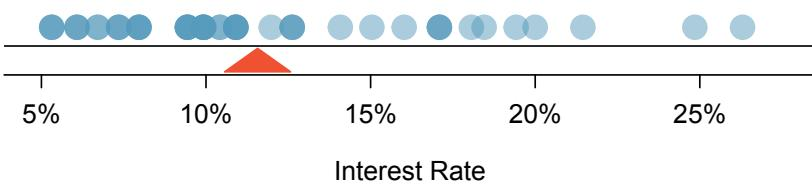
\includegraphics{_page_41_Figure_9.jpeg}

Figura 2.3: Un diagrama de puntos de la tasa de interés para el conjunto
de datos loan50. La media de la distribución se muestra como un
triángulo rojo.

1Las respuestas pueden variar. Los diagramas de dispersión son útiles
para detectar rápidamente asociaciones que relacionan variables, ya sea
que esas asociaciones vengan en forma de tendencias simples o que esas
relaciones sean más complejas.

2Considere el caso en el que su eje vertical representa algo ``bueno'' y
su eje horizontal representa algo que solo es bueno con moderación. La
salud y el consumo de agua se ajustan a esta descripción: necesitamos
algo de agua para sobrevivir, pero consumimos demasiado y se vuelve
tóxico y puede matar a una persona.

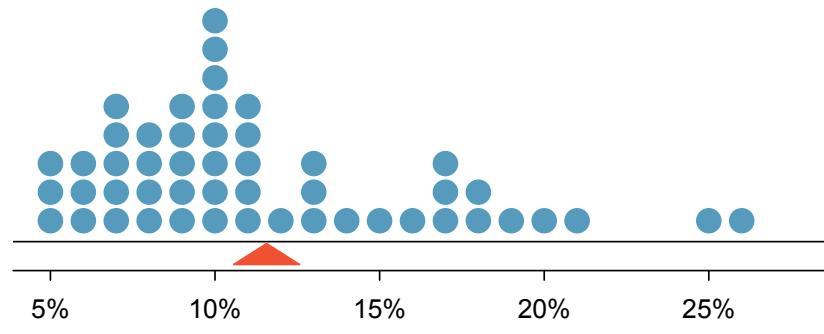
\includegraphics{_page_42_Figure_1.jpeg}

Tasa de Interés, Redondeada al Porcentaje Más Cercano

Figura 2.4: Un diagrama de puntos apilado de la tasa de interés para el
conjunto de datos loan50. Las tasas se han redondeado al porcentaje más
cercano en este diagrama, y la media de la distribución se muestra como
un triángulo rojo.

La media, a menudo llamada el promedio, es una forma común de medir el
centro de una distribución de datos. Para calcular la tasa de interés
media, sumamos todas las tasas de interés y dividimos por el número de
observaciones:

\[\bar{x} = \frac{10.90\% + 9.92\% + 26.30\% + \dots + 6.08\%}{50} = 11.57\%\]

La media muestral a menudo se etiqueta como ¯x. La letra x se usa como
un marcador de posición genérico para la variable de interés, la tasa de
interés, y la barra sobre la x comunica que estamos viendo la tasa de
interés promedio, que para estos 50 préstamos fue del 11.57\%. Es útil
pensar en la media como el punto de equilibrio de la distribución, y se
muestra como un triángulo en las Figuras \hyperref[page-41-3]{2.3} y
\hyperref[page-42-0]{2.4.}

\section{\texorpdfstring{\textbf{MEDIA}}{MEDIA}}\label{media}

La media muestral puede calcularse como la suma de los valores
observados dividida entre el número de observaciones:

\[
\bar{x} = \frac{x\_1 + x\_2 + \dots + x\_n}{n}
\]

donde x1, x2, . . . , xn representan los n valores observados.

\section{\texorpdfstring{\textbf{PRÁCTICA GUIADA
2.4}}{PRÁCTICA GUIADA 2.4}}\label{pruxe1ctica-guiada-2.4}

Examina la ecuación para la media. ¿A qué corresponde x1? ¿Y x2? ¿Puedes
inferir un significado general a lo que xi podría
representar?\hyperref[page-42-1]{3}

\paragraph{\texorpdfstring{\textbf{PRÁCTICA GUIADA
2.5}}{PRÁCTICA GUIADA 2.5}}\label{pruxe1ctica-guiada-2.5}

¿Cuál era n en esta muestra de préstamos?\hyperref[page-42-2]{4}

El conjunto de datos loan50 representa una muestra de una población más
grande de préstamos realizados a través de Lending Club. Podríamos
calcular una media para esta población de la misma manera que la media
muestral. Sin embargo, la media poblacional tiene una etiqueta especial:
µ. El símbolo µ es la letra griega mu y representa el promedio de todas
las observaciones en la población. A veces se usa un subíndice, como x,
para representar a qué variable se refiere la media poblacional, p.~ej.
µx. A menudo, es demasiado costoso medir la media poblacional con
precisión, por lo que a menudo estimamos µ usando la media muestral, ¯x.

3x1 corresponde a la tasa de interés para el primer préstamo en la
muestra (10.90\%), x2 a la tasa de interés del segundo préstamo (9.92\%)
y xi corresponde a la tasa de interés para el i-ésimo préstamo en el
conjunto de datos. Por ejemplo, si i = 4, entonces estamos examinando
x4, que se refiere a la cuarta observación en el conjunto de datos.

4El tamaño de la muestra fue n = 50.

\section{\texorpdfstring{\textbf{EJEMPLO
2.6}}{EJEMPLO 2.6}}\label{ejemplo-2.6}

La tasa de interés promedio en todos los préstamos en la población se
puede estimar utilizando los datos de la muestra. Según la muestra de 50
préstamos, ¿cuál sería una estimación razonable de µx, la tasa de
interés media para todos los préstamos en el conjunto de datos completo?

La media muestral, 11.57\%, proporciona una estimación aproximada de µx.
Si bien no es perfecto, esta es nuestra mejor conjetura de la tasa de
interés promedio de todos los préstamos en la población bajo estudio.

En el Capítulo \hyperref[page-167-0]{5} y más adelante, desarrollaremos
herramientas para caracterizar la precisión de las estimaciones
puntuales como la media muestral. Como habrás adivinado, las
estimaciones puntuales basadas en muestras más grandes tienden a ser más
precisas que las basadas en muestras más pequeñas.

\section{\texorpdfstring{\textbf{EJEMPLO
2.7}}{EJEMPLO 2.7}}\label{ejemplo-2.7}

La media es útil porque nos permite reescalar o estandarizar una métrica
en algo más fácil de interpretar y comparar. Proporciona 2 ejemplos
donde la media es útil para hacer comparaciones.

\begin{enumerate}
\def\labelenumi{\arabic{enumi}.}
\tightlist
\item
  Nos gustaría entender si un nuevo fármaco es más eficaz para tratar
  los ataques de asma que el fármaco estándar. Se establece un ensayo
  con 1500 adultos, donde 500 reciben el nuevo fármaco y 1000 reciben un
  fármaco estándar en el grupo de control:
\end{enumerate}

\begin{longtable}[]{@{}lll@{}}
\toprule\noalign{}
& Nuevo fármaco & Fármaco estándar \\
\midrule\noalign{}
\endhead
\bottomrule\noalign{}
\endlastfoot
Número de pacientes & 500 & 1000 \\
Ataques totales de asma & 200 & 300 \\
\end{longtable}

Comparar los recuentos brutos de 200 a 300 ataques de asma haría parecer
que el nuevo fármaco es mejor, pero esto es un artefacto del tamaño
desigual de los grupos. En cambio, deberíamos observar el número medio
de ataques de asma por paciente en cada grupo:

Nuevo fármaco: 200/500 = 0.4 Fármaco estándar: 300/1000 = 0.3

El fármaco estándar tiene un número medio de ataques de asma por
paciente menor que la media del grupo de tratamiento.

\begin{enumerate}
\def\labelenumi{\arabic{enumi}.}
\setcounter{enumi}{1}
\tightlist
\item
  Emilio abrió un camión de comida el año pasado donde vende burritos, y
  su negocio se ha estabilizado en los últimos 3 meses. Durante ese
  período de 3 meses, ha ganado \$11,000 mientras trabajaba 625 horas.
  Las ganancias medias por hora de Emilio proporcionan una estadística
  útil para evaluar si su empresa, al menos desde una perspectiva
  financiera, merece la pena:
\end{enumerate}

\begin{quote}
\$11000 625 horas = \$17.60 por hora
\end{quote}

Al conocer su salario medio por hora, Emilio ha convertido sus ganancias
en una unidad estándar que es más fácil de comparar con muchos otros
trabajos que podría considerar.

\paragraph{\texorpdfstring{\textbf{EJEMPLO
2.8}}{EJEMPLO 2.8}}\label{ejemplo-2.8}

Supongamos que queremos calcular el ingreso medio por persona en los EE.
UU. Para ello, podríamos pensar en calcular la media de los ingresos per
cápita en los 3142 condados del conjunto de datos del condado. ¿Cuál
sería un mejor enfoque?

El conjunto de datos del condado es especial en el sentido de que cada
condado representa en realidad a muchas personas individuales. Si
simplemente promediáramos la variable de ingresos, estaríamos tratando a
los condados con 5000 y 5,000,000 de residentes por igual en los
cálculos. En cambio, deberíamos calcular el ingreso total para cada
condado, sumar los totales de todos los condados y luego dividir por el
número de personas en todos los condados. Si completáramos estos pasos
con los datos del condado, encontraríamos que el ingreso per cápita para
los EE. UU. es de \$30,861. Si hubiéramos calculado la media simple del
ingreso per cápita entre los condados, ¡el resultado habría sido de solo
\$26,093!

Este ejemplo utilizó lo que se llama una media ponderada. Para obtener
más información sobre este tema, consulta el siguiente suplemento en
línea sobre medias ponderadas
\href{http://www.openintro.org/redirect.php?go=stat_wtd_mean&referrer=os4_pdf}{openintro.org/d?file=stat}
wtd mean.

\section{\texorpdfstring{\textbf{2.1.3 Histogramas y
forma}}{2.1.3 Histogramas y forma}}\label{histogramas-y-forma}

Los diagramas de puntos muestran el valor exacto para cada observación.
Esto es útil para conjuntos de datos pequeños, pero pueden volverse
difíciles de leer con muestras más grandes. En lugar de mostrar el valor
de cada observación, preferimos pensar en el valor como perteneciente a
un intervalo. Por ejemplo, en el conjunto de datos loan50, creamos una
tabla de recuentos para el número de préstamos con tasas de interés
entre 5.0\% y 7.5\%, luego el número de préstamos con tasas entre 7.5\%
y 10.0\%, y así sucesivamente. Las observaciones que caen en el límite
de un intervalo (por ejemplo, 10.00\%) se asignan al intervalo inferior.
Esta tabulación se muestra en la Figura \hyperref[page-44-0]{2.5.} Estos
recuentos agrupados se representan como barras en la Figura
\hyperref[page-44-1]{2.6} en lo que se llama un histograma, que se
asemeja a una versión más agrupada del diagrama de puntos apilados que
se muestra en la Figura \hyperref[page-42-0]{2.4.}

\begin{longtable}[]{@{}
  >{\raggedright\arraybackslash}p{(\columnwidth - 12\tabcolsep) * \real{0.1429}}
  >{\raggedright\arraybackslash}p{(\columnwidth - 12\tabcolsep) * \real{0.1429}}
  >{\raggedright\arraybackslash}p{(\columnwidth - 12\tabcolsep) * \real{0.1429}}
  >{\raggedright\arraybackslash}p{(\columnwidth - 12\tabcolsep) * \real{0.1429}}
  >{\raggedright\arraybackslash}p{(\columnwidth - 12\tabcolsep) * \real{0.1429}}
  >{\raggedright\arraybackslash}p{(\columnwidth - 12\tabcolsep) * \real{0.1429}}
  >{\raggedright\arraybackslash}p{(\columnwidth - 12\tabcolsep) * \real{0.1429}}@{}}
\toprule\noalign{}
\begin{minipage}[b]{\linewidth}\raggedright
Tasa de interés
\end{minipage} & \begin{minipage}[b]{\linewidth}\raggedright
5.0\% - 7.5\%
\end{minipage} & \begin{minipage}[b]{\linewidth}\raggedright
7.5\% - 10.0\%
\end{minipage} & \begin{minipage}[b]{\linewidth}\raggedright
10.0\% - 12.5\%
\end{minipage} & \begin{minipage}[b]{\linewidth}\raggedright
12.5\% - 15.0\%
\end{minipage} & \begin{minipage}[b]{\linewidth}\raggedright
· · ·
\end{minipage} & \begin{minipage}[b]{\linewidth}\raggedright
25.0\% - 27.5\%
\end{minipage} \\
\midrule\noalign{}
\endhead
\bottomrule\noalign{}
\endlastfoot
Recuento & 11 & 15 & 8 & 4 & · · · & 1 \\
\end{longtable}

Figura 2.5: Recuentos para los datos de la tasa de interés agrupados.

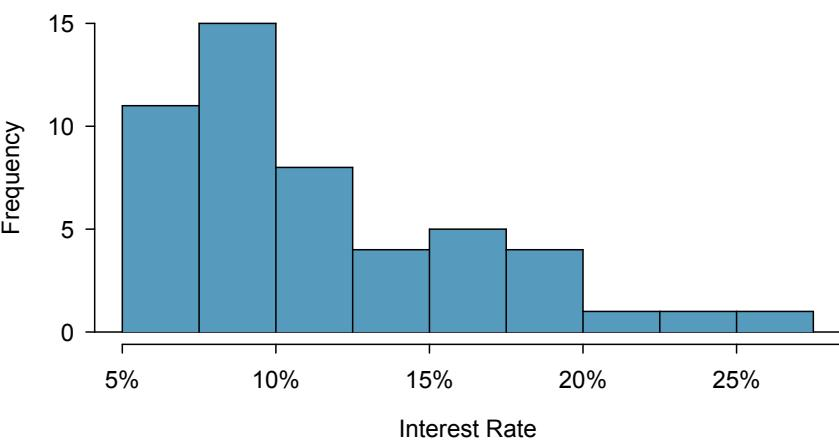
\includegraphics{_page_44_Figure_5.jpeg}

Figura 2.6: Un histograma de la tasa de interés. Esta distribución está
fuertemente sesgada hacia la derecha.

Los histogramas proporcionan una vista de la densidad de los datos. Las
barras más altas representan dónde los datos son relativamente más
comunes. Por ejemplo, hay muchos más préstamos con tasas entre el 5\% y
el 10\% que préstamos con tasas entre el 20\% y el 25\% en el conjunto
de datos. Las barras facilitan ver cómo cambia la densidad de los datos
en relación con la tasa de interés.

Los histogramas son especialmente convenientes para comprender la forma
de la distribución de los datos. La Figura \hyperref[page-44-1]{2.6}
sugiere que la mayoría de los préstamos tienen tasas por debajo del
15\%, mientras que solo un puñado de préstamos tienen tasas por encima
del 20\%. Cuando los datos se extienden hacia la derecha de esta manera
y tienen una cola derecha más larga, se dice que la forma está sesgada a
la derecha. \hyperref[page-44-2]{5}

Los conjuntos de datos con la característica inversa, una cola larga y
delgada a la izquierda, se dice que están sesgados a la izquierda.
También decimos que tal distribución tiene una cola larga a la
izquierda. Los conjuntos de datos que muestran una atenuación
aproximadamente igual en ambas direcciones se llaman simétricos.

\paragraph{\texorpdfstring{\textbf{COLAS LARGAS PARA IDENTIFICAR EL
SESGO}}{COLAS LARGAS PARA IDENTIFICAR EL SESGO}}\label{colas-largas-para-identificar-el-sesgo}

Cuando los datos se extienden en una dirección, la distribución tiene
una cola larga. Si una distribución tiene una cola larga a la izquierda,
está sesgada a la izquierda. Si una distribución tiene una cola larga a
la derecha, está sesgada a la derecha.

5Otras formas de describir los datos que están sesgados a la derecha:
sesgados hacia la derecha, sesgados hacia el extremo superior o sesgados
hacia el extremo positivo.

Echa un vistazo a los diagramas de puntos en las Figuras
\hyperref[page-41-3]{2.3} y \hyperref[page-42-0]{2.4.} ¿Puedes ver el
sesgo en los datos? ¿Es más fácil ver el sesgo en este histograma o en
los diagramas de puntos?\hyperref[page-45-0]{6}

\textbf{PRÁCTICA GUIADA 2.10}

Además de la media (ya que fue etiquetada), ¿qué puedes ver en los
diagramas de puntos que no puedes ver en el
histograma?\hyperref[page-45-1]{7}

Además de observar si una distribución está sesgada o es simétrica, los
histogramas se pueden utilizar para identificar modos. Un modo está
representado por un pico prominente en la distribución. Solo hay un pico
prominente en el histograma del monto del préstamo.

Una definición de modo que a veces se enseña en las clases de
matemáticas es el valor con más ocurrencias en el conjunto de datos. Sin
embargo, para muchos conjuntos de datos del mundo real, es común no
tener observaciones con el mismo valor en un conjunto de datos, lo que
hace que esta definición no sea práctica en el análisis de datos.

La Figura \hyperref[page-45-2]{2.7} muestra histogramas que tienen uno,
dos o tres picos prominentes. Tales distribuciones se llaman unimodales,
bimodales y multimodales, respectivamente. Cualquier distribución con
más de 2 picos prominentes se llama multimodal. Observa que había un
pico prominente en la distribución unimodal con un segundo pico menos
prominente que no se contó ya que solo difiere de sus intervalos vecinos
en unas pocas observaciones.

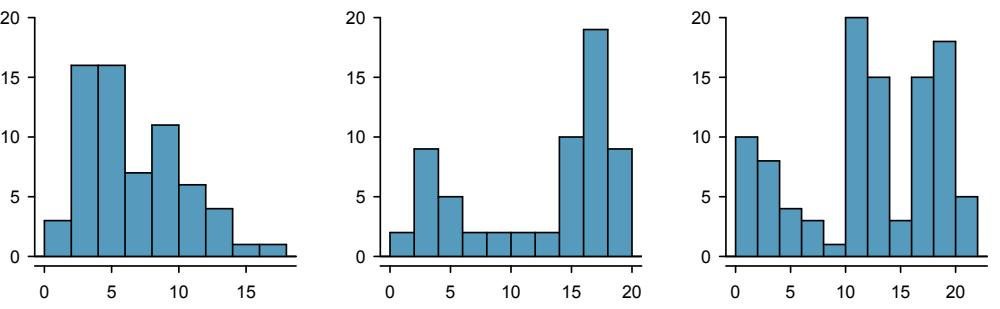
\includegraphics{_page_45_Figure_8.jpeg}

Figura 2.7: Contando solo los picos prominentes, las distribuciones son
(de izquierda a derecha) unimodal, bimodal y multimodal. Ten en cuenta
que hemos dicho que la gráfica de la izquierda es unimodal
intencionalmente. Esto se debe a que estamos contando picos prominentes,
no solo cualquier pico.

\section{\texorpdfstring{\textbf{EJEMPLO
2.11}}{EJEMPLO 2.11}}\label{ejemplo-2.11}

La Figura \hyperref[page-44-1]{2.6} revela solo un modo prominente en la
tasa de interés. ¿Es la distribución unimodal, bimodal o multimodal?

Unimodal. Recuerda que uni significa 1 (piensa en monociclos). De manera
similar, bi significa 2 (piensa en bicicletas). Esperamos que se invente
un multiciclo para completar esta analogía.

\section{\texorpdfstring{\textbf{PRÁCTICA GUIADA
2.12}}{PRÁCTICA GUIADA 2.12}}\label{pruxe1ctica-guiada-2.12}

Se tomaron medidas de altura de estudiantes jóvenes y profesores adultos
en una escuela primaria K-3. ¿Cuántos modos esperaría encontrar en este
conjunto de datos de altura?\hyperref[page-45-3]{8}

La búsqueda de modos no se trata de encontrar una respuesta clara y
correcta sobre el número de modos en una distribución, razón por la cual
``prominente'' no está rigurosamente definido en este libro. La parte
más importante de este examen es comprender mejor sus datos.

6La asimetría es visible en los tres gráficos, aunque el diagrama de
puntos plano es el menos útil. El diagrama de puntos apilados y el
histograma son visualizaciones útiles para identificar la asimetría.

7Las tasas de interés de los préstamos individuales.

8Podrían haber dos grupos de altura visibles en el conjunto de datos:
uno de los estudiantes y otro de los adultos. Es decir, los datos son
probablemente bimodales.

\section{\texorpdfstring{\textbf{2.1.4 Varianza y desviación
estándar}}{2.1.4 Varianza y desviación estándar}}\label{varianza-y-desviaciuxf3n-estuxe1ndar}

La media se introdujo como un método para describir el centro de un
conjunto de datos, y la variabilidad en los datos también es importante.
Aquí, presentamos dos medidas de variabilidad: la varianza y la
desviación estándar. Ambas son muy útiles en el análisis de datos,
aunque sus fórmulas son un poco tediosas de calcular a mano. La
desviación estándar es la más fácil de comprender de las dos, y describe
aproximadamente qué tan lejos está la observación típica de la media.

Llamamos a la distancia de una observación desde su media su desviación.
A continuación, se muestran las desviaciones para las observaciones 1ª,
2ª, 3ª y 50ª en la variable de tasa de interés:

\[\begin{aligned} x\_1 - \bar{x} &= 10.90 - 11.57 = -0.67\\ x\_2 - \bar{x} &= 9.92 - 11.57 = -1.65\\ x\_3 - \bar{x} &= 26.30 - 11.57 = 14.73\\ &\vdots\\ x\_{50} - \bar{x} &= 6.08 - 11.57 = -5.49 \end{aligned}\]

Si elevamos al cuadrado estas desviaciones y luego sacamos un promedio,
el resultado es igual a la varianza de la muestra, denotada por s 2 :

\[\begin{split} s^2 &= \frac{(-0.67)^2 + (-1.65)^2 + (14.73)^2 + \dots + (-5.49)^2}{50 - 1} \\ &= \frac{0.45 + 2.72 + 216.97 + \dots + 30.14}{49} \\ &= 25.52 \end{split}\]

Dividimos por n − 1, en lugar de dividir por n, al calcular la varianza
de una muestra; hay algunos matices matemáticos aquí, pero el resultado
final es que hacer esto hace que esta estadística sea un poco más
confiable y útil.

Observe que elevar al cuadrado las desviaciones hace dos cosas. Primero,
hace que los valores grandes sean relativamente mucho más grandes, como
se ve al comparar (−0.67)2 , (−1.65)2 , (14.73)2 y (−5.49)2 . En segundo
lugar, elimina cualquier signo negativo.

La desviación estándar se define como la raíz cuadrada de la varianza:

\[s = \sqrt{25.52} = 5.05\]

Si bien a menudo se omite, se puede agregar un subíndice de x a la
varianza y la desviación estándar, es decir, s 2 x y sx , si es útil
como recordatorio de que estas son la varianza y la desviación estándar
de las observaciones representadas por x1 , x2 , \ldots, xn .

\section{\texorpdfstring{\textbf{VARIANZA Y DESVIACIÓN
ESTÁNDAR}}{VARIANZA Y DESVIACIÓN ESTÁNDAR}}\label{varianza-y-desviaciuxf3n-estuxe1ndar-1}

La varianza es la distancia promedio al cuadrado desde la media. La
desviación estándar es la raíz cuadrada de la varianza. La desviación
estándar es útil cuando se considera qué tan lejos están distribuidos
los datos de la media.

La desviación estándar representa la desviación típica de las
observaciones con respecto a la media. Generalmente, alrededor del 70\%
de los datos estarán dentro de una desviación estándar de la media y
alrededor del 95\% estarán dentro de dos desviaciones estándar. Sin
embargo, como se ve en las Figuras \hyperref[page-47-0]{2.8} y
\hyperref[page-47-1]{2.9,} estos porcentajes no son reglas estrictas.

Al igual que la media, los valores de la población para la varianza y la
desviación estándar tienen símbolos especiales: σ 2 para la varianza y σ
para la desviación estándar. El símbolo σ es la letra griega sigma.

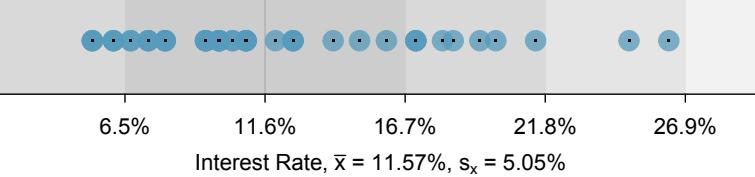
\includegraphics{_page_47_Figure_1.jpeg}

Figura 2.8: Para la variable de tasa de interés, 34 de los 50 préstamos
(68\%) tenían tasas de interés dentro de 1 desviación estándar de la
media, y 48 de los 50 préstamos (96\%) tenían tasas dentro de 2
desviaciones estándar. Generalmente, alrededor del 70\% de los datos
están dentro de 1 desviación estándar de la media y el 95\% dentro de 2
desviaciones estándar, aunque esto está lejos de ser una regla estricta.

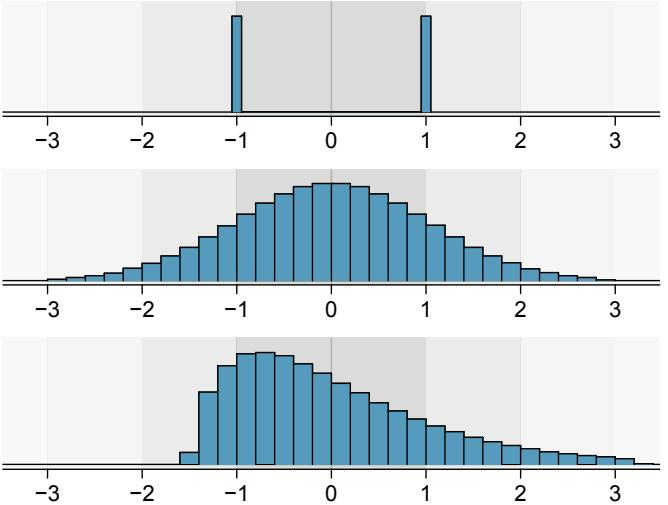
\includegraphics{_page_47_Figure_3.jpeg}

Figura 2.9: Tres distribuciones de población muy diferentes con la misma
media µ = 0 y desviación estándar σ = 1.

\section{\texorpdfstring{\textbf{PRÁCTICA GUIADA
2.13}}{PRÁCTICA GUIADA 2.13}}\label{pruxe1ctica-guiada-2.13}

En la página \hyperref[page-44-1]{45,} se introdujo el concepto de forma
de una distribución. Una buena descripción de la forma de una
distribución debería incluir la modalidad e indicar si la distribución
es simétrica o sesgada hacia un lado. Usando la Figura
\hyperref[page-47-1]{2.9} como ejemplo, explica por qué tal descripción
es importante.\hyperref[page-47-2]{9}

\paragraph{\texorpdfstring{\textbf{EJEMPLO
2.14}}{EJEMPLO 2.14}}\label{ejemplo-2.14}

Describe la distribución de la variable de tasa de interés utilizando el
histograma en la Figura \hyperref[page-44-1]{2.6.} La descripción debe
incorporar el centro, la variabilidad y la forma de la distribución, y
también debe ubicarse en contexto. También observa cualquier caso
especialmente inusual.

La distribución de las tasas de interés es unimodal y está sesgada hacia
el extremo superior. Muchas de las tasas se encuentran cerca de la media
en 11.57\%, y la mayoría se encuentra dentro de una desviación estándar
(5.05\%) de la media. Hay algunas tasas de interés excepcionalmente
grandes en la muestra que están por encima del 20\%.

En la práctica, la varianza y la desviación estándar a veces se utilizan
como un medio para un fin, donde el ``fin'' es poder estimar con
precisión la incertidumbre asociada con un estadístico de muestra. Por
ejemplo, en el Capítulo \hyperref[page-167-0]{5} la desviación estándar
se utiliza en cálculos que nos ayudan a comprender cuánto varía la media
de una muestra de una muestra a otra.

9La Figura \hyperref[page-47-1]{2.9} muestra tres distribuciones que se
ven bastante diferentes, pero todas tienen la misma media, varianza y
desviación estándar. Usando la modalidad, podemos distinguir entre el
primer gráfico (bimodal) y los dos últimos (unimodal). Usando la
asimetría, podemos distinguir entre el último gráfico (sesgado a la
derecha) y los dos primeros. Si bien una imagen, como un histograma,
cuenta una historia más completa, podemos usar la modalidad y la forma
(simetría/sesgo) para caracterizar información básica sobre una
distribución.

\section{\texorpdfstring{\textbf{2.1.5 Diagramas de caja, cuartiles y la
mediana}}{2.1.5 Diagramas de caja, cuartiles y la mediana}}\label{diagramas-de-caja-cuartiles-y-la-mediana}

Un diagrama de caja resume un conjunto de datos utilizando cinco
estadísticas mientras que también grafica observaciones inusuales. La
Figura \hyperref[page-48-0]{2.10} proporciona un diagrama de puntos
vertical junto con un diagrama de caja de la variable de tasa de interés
del conjunto de datos loan50.

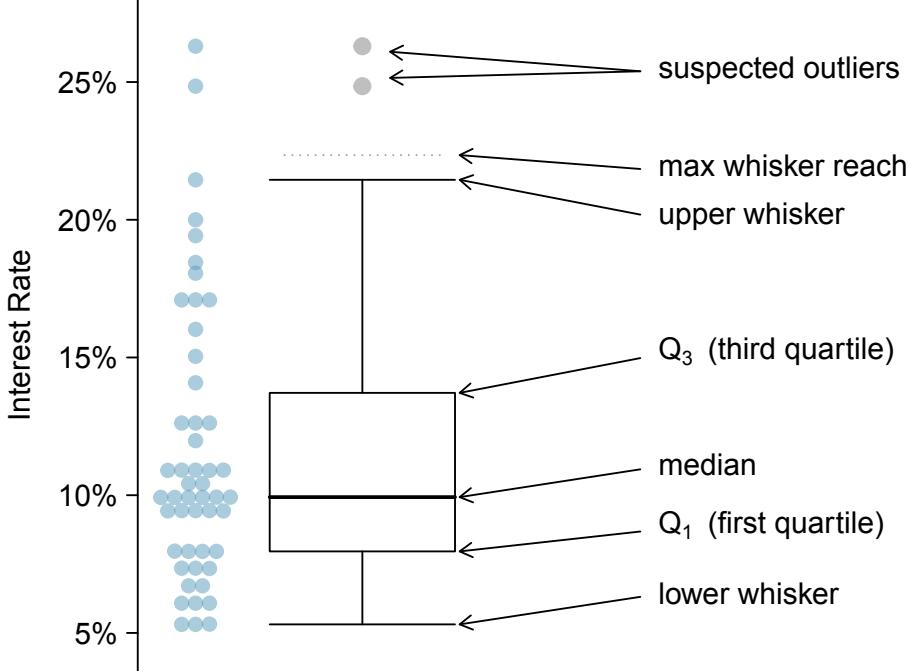
\includegraphics{_page_48_Figure_3.jpeg}

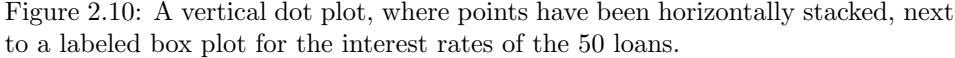
\includegraphics{_page_48_Figure_4.jpeg}

El primer paso para construir un diagrama de caja es dibujar una línea
oscura que denote la mediana, que divide los datos por la mitad. La
Figura \hyperref[page-48-0]{2.10} muestra que el 50\% de los datos cae
por debajo de la mediana y el otro 50\% cae por encima de la mediana.
Hay 50 préstamos en el conjunto de datos (un número par), por lo que los
datos se dividen perfectamente en dos grupos de 25. Tomamos la mediana
en este caso como el promedio de las dos observaciones más cercanas al
percentil 50, que resultan ser el mismo valor en este conjunto de datos:
(9.93\% + 9.93\%)/2 = 9.93\%. Cuando hay un número impar de
observaciones, habrá exactamente una observación que divida los datos en
dos mitades, y en tal caso esa observación es la mediana (no se necesita
promedio).

\section{\texorpdfstring{\textbf{MEDIANA: EL NÚMERO DE EN
MEDIO}}{MEDIANA: EL NÚMERO DE EN MEDIO}}\label{mediana-el-nuxfamero-de-en-medio}

Si los datos están ordenados de menor a mayor, la mediana es la
observación justo en el medio. Si hay un número par de observaciones,
habrá dos valores en el medio, y la mediana se toma como su promedio.

El segundo paso en la construcción de un diagrama de caja es dibujar un
rectángulo para representar el 50\% central de los datos. La longitud
total de la caja, que se muestra verticalmente en la Figura
\hyperref[page-48-0]{2.10,} se llama rango intercuartílico (IQR, para
abreviar). Éste, al igual que la desviación estándar, es una medida de
la variabilidad de los datos. Cuanto más variables sean los datos, mayor
tenderá a ser la desviación estándar y el IQR. Los dos límites de la
caja se llaman primer cuartil (el percentil 25, es decir, el 25\% de los
datos cae por debajo de este valor) y el tercer cuartil (el percentil
75), y estos a menudo se etiquetan como Q1 y Q3, respectivamente.

\section{\texorpdfstring{\textbf{RANGO INTERCUARTÍLICO
(IQR)}}{RANGO INTERCUARTÍLICO (IQR)}}\label{rango-intercuartuxedlico-iqr}

El IQR es la longitud de la caja en un diagrama de caja. Se calcula como

IQR = Q3 − Q1

donde Q1 y Q3 son los percentiles 25 y 75.

\paragraph{\texorpdfstring{\textbf{PRÁCTICA GUIADA
2.15}}{PRÁCTICA GUIADA 2.15}}\label{pruxe1ctica-guiada-2.15}

¿Qué porcentaje de los datos cae entre Q1 y la mediana? ¿Qué porcentaje
está entre la mediana y Q3? \hyperref[page-49-0]{10}

Extendiéndose desde la caja, los bigotes intentan capturar los datos
fuera de la caja. Sin embargo, nunca se permite que su alcance sea
superior a 1,5 × IQR. Capturan todo dentro de este alcance. En la Figura
\hyperref[page-48-0]{2.10,} el bigote superior no se extiende hasta los
dos últimos puntos, que están más allá de Q3 + 1,5 × IQR, por lo que se
extiende solo hasta el último punto por debajo de este límite. El bigote
inferior se detiene en el valor más bajo, 5,31\%, ya que no hay datos
adicionales para alcanzar; el límite del bigote inferior no se muestra
en la figura porque el gráfico no se extiende hasta Q1 −1,5×IQR. En
cierto sentido, la caja es como el cuerpo del diagrama de caja y los
bigotes son como sus brazos que intentan alcanzar el resto de los datos.

Cualquier observación que se encuentre más allá de los bigotes se
etiqueta con un punto. El propósito de etiquetar estos puntos, en lugar
de extender los bigotes a los valores mínimo y máximo observados, es
ayudar a identificar cualquier observación que parezca inusualmente
distante del resto de los datos. Las observaciones inusualmente
distantes se denominan valores atípicos. En este caso, sería razonable
clasificar las tasas de interés de 24,85\% y 26,30\% como valores
atípicos, ya que están numéricamente distantes de la mayoría de los
datos.

\paragraph{\texorpdfstring{\textbf{LOS VALORES ATÍPICOS SON
EXTREMOS}}{LOS VALORES ATÍPICOS SON EXTREMOS}}\label{los-valores-atuxedpicos-son-extremos}

Un valor atípico es una observación que parece extrema en relación con
el resto de los datos.

El examen de los datos en busca de valores atípicos tiene muchos
propósitos útiles, que incluyen

\begin{itemize}
\tightlist
\item
  \begin{enumerate}
  \def\labelenumi{\arabic{enumi}.}
  \tightlist
  \item
    Identificar una fuerte asimetría en la distribución.
  \end{enumerate}
\item
  \begin{enumerate}
  \def\labelenumi{\arabic{enumi}.}
  \setcounter{enumi}{1}
  \tightlist
  \item
    Identificar posibles errores en la recopilación o entrada de datos.
  \end{enumerate}
\item
  \begin{enumerate}
  \def\labelenumi{\arabic{enumi}.}
  \setcounter{enumi}{2}
  \tightlist
  \item
    Proporcionar información sobre propiedades interesantes de los
    datos.
  \end{enumerate}
\end{itemize}

\paragraph{\texorpdfstring{\textbf{PRÁCTICA GUIADA
2.16}}{PRÁCTICA GUIADA 2.16}}\label{pruxe1ctica-guiada-2.16}

Usando la Figura \hyperref[page-48-0]{2.10,} estime los siguientes
valores para la tasa de interés en el conjunto de datos loan50: (a) Q1,
(b) Q3 y (c) IQR.\hyperref[page-49-1]{11}

10Dado que Q1 y Q3 capturan el 50\% central de los datos y la mediana
divide los datos por la mitad, el 25\% de los datos cae entre Q1 y la
mediana, y otro 25\% cae entre la mediana y Q3.

11Estas estimaciones visuales variarán un poco de una persona a otra: Q1
= 8\%, Q3 = 14\%, IQR = Q3 −Q1 = 6\%. (Los valores verdaderos: Q1 =
7,96\%, Q3 = 13,72\%, IQR = 5,76\%.)

\section{\texorpdfstring{\textbf{2.1.6 Estadísticas
robustas}}{2.1.6 Estadísticas robustas}}\label{estaduxedsticas-robustas}

¿Cómo se ven afectadas las estadísticas de muestra del conjunto de datos
de la tasa de interés por la observación, 26,3\%? ¿Qué habría pasado si
este préstamo hubiera sido solo del 15\%? ¿Qué pasaría con estas
estadísticas resumidas si la observación del 26,3\% hubiera sido aún
mayor, digamos, del 35\%? Estos escenarios se representan junto con los
datos originales en la Figura \hyperref[page-50-0]{2.11,} y las
estadísticas de muestra se calculan en cada escenario en la Figura
\hyperref[page-50-1]{2.12.}

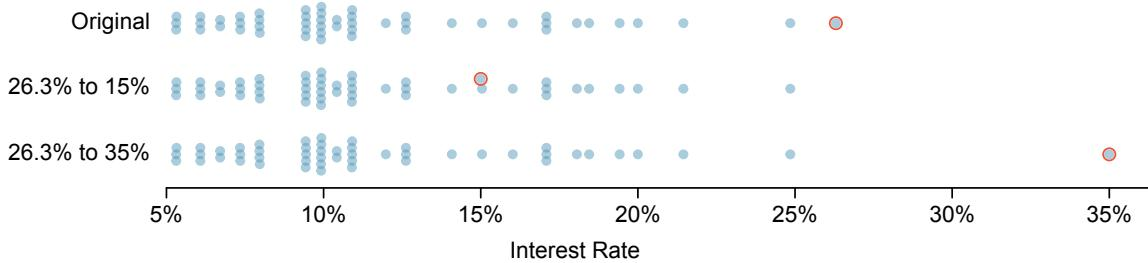
\includegraphics{_page_50_Figure_3.jpeg}

Figura 2.11: Gráficos de puntos de los datos originales de la tasa de
interés y dos conjuntos de datos modificados.

\begin{longtable}[]{@{}
  >{\raggedright\arraybackslash}p{(\columnwidth - 10\tabcolsep) * \real{0.5000}}
  >{\raggedright\arraybackslash}p{(\columnwidth - 10\tabcolsep) * \real{0.1125}}
  >{\raggedright\arraybackslash}p{(\columnwidth - 10\tabcolsep) * \real{0.0875}}
  >{\raggedright\arraybackslash}p{(\columnwidth - 10\tabcolsep) * \real{0.1500}}
  >{\raggedright\arraybackslash}p{(\columnwidth - 10\tabcolsep) * \real{0.0875}}
  >{\raggedright\arraybackslash}p{(\columnwidth - 10\tabcolsep) * \real{0.0625}}@{}}
\toprule\noalign{}
\begin{minipage}[b]{\linewidth}\raggedright
\end{minipage} & \begin{minipage}[b]{\linewidth}\raggedright
robusto
\end{minipage} & \begin{minipage}[b]{\linewidth}\raggedright
\end{minipage} & \begin{minipage}[b]{\linewidth}\raggedright
no robusto
\end{minipage} & \begin{minipage}[b]{\linewidth}\raggedright
\end{minipage} & \begin{minipage}[b]{\linewidth}\raggedright
\end{minipage} \\
\midrule\noalign{}
\endhead
\bottomrule\noalign{}
\endlastfoot
escenario & mediana & IQR & ¯x & s & \\
datos originales de la tasa de interés & 9.93\% & 5.76\% & 11.57\% &
5.05\% & \\
mover 26.3\% → 15\% & 9.93\% & 5.76\% & 11.34\% & 4.61\% & \\
mover 26.3\% → 35\% & 9.93\% & 5.76\% & 11.74\% & 5.68\% & \\
\end{longtable}

Figura 2.12: Una comparación de cómo la mediana, el IQR, la media (¯x) y
la desviación estándar (s) cambian si una observación extrema de la
variable de la tasa de interés hubiera sido diferente.

\section{\texorpdfstring{\textbf{PRÁCTICA GUIADA
2.17}}{PRÁCTICA GUIADA 2.17}}\label{pruxe1ctica-guiada-2.17}

\begin{enumerate}
\def\labelenumi{(\alph{enumi})}
\tightlist
\item
  ¿Qué se ve más afectado por las observaciones extremas, la media o la
  mediana? La Figura \hyperref[page-50-1]{2.12} puede ser útil. (b) ¿La
  desviación estándar o el IQR se ven más afectados por las
  observaciones extremas?\hyperref[page-50-2]{12}
\end{enumerate}

La mediana y el IQR se denominan estadísticas robustas porque las
observaciones extremas tienen poco efecto sobre sus valores: mover el
valor más extremo generalmente tiene poca influencia en estas
estadísticas. Por otro lado, la media y la desviación estándar están más
influenciadas por los cambios en las observaciones extremas, lo que
puede ser importante en algunas situaciones.

\paragraph{\texorpdfstring{\textbf{EJEMPLO
2.18}}{EJEMPLO 2.18}}\label{ejemplo-2.18}

La mediana y el IQR no cambiaron en los tres escenarios en la Figura
\hyperref[page-50-1]{2.12.} ¿Por qué podría ser este el caso?

La mediana y el IQR solo son sensibles a los números cercanos a Q1, la
mediana y Q3. Dado que los valores en estas regiones son estables en los
tres conjuntos de datos, las estimaciones de la mediana y el IQR también
son estables.

\paragraph{\texorpdfstring{\textbf{PRÁCTICA GUIADA
2.19}}{PRÁCTICA GUIADA 2.19}}\label{pruxe1ctica-guiada-2.19}

La distribución de los montos de los préstamos en el conjunto de datos
loan50 está sesgada a la derecha, con algunos préstamos grandes que
permanecen en la cola derecha. Si quisiera comprender el tamaño típico
del préstamo, ¿debería estar más interesado en la media o la
mediana?\hyperref[page-50-3]{13}

12(a) La media se ve más afectada. (b) La desviación estándar se ve más
afectada. Se proporcionan explicaciones completas en el material que
sigue a la Práctica Guiada \hyperref[page-50-4]{2.17.}

13¡Las respuestas variarán! Si simplemente buscamos comprender cómo es
un préstamo individual típico, la mediana es probablemente más útil. Sin
embargo, si el objetivo es comprender algo que se escala bien, como la
cantidad total de dinero que podríamos necesitar tener a mano si
ofreciéramos 1000 préstamos, entonces la media sería más útil.

\section{\texorpdfstring{\textbf{2.1.7 Transformación de datos (tema
especial)}}{2.1.7 Transformación de datos (tema especial)}}\label{transformaciuxf3n-de-datos-tema-especial}

Cuando los datos están muy fuertemente sesgados, a veces los
transformamos para que sean más fáciles de modelar.

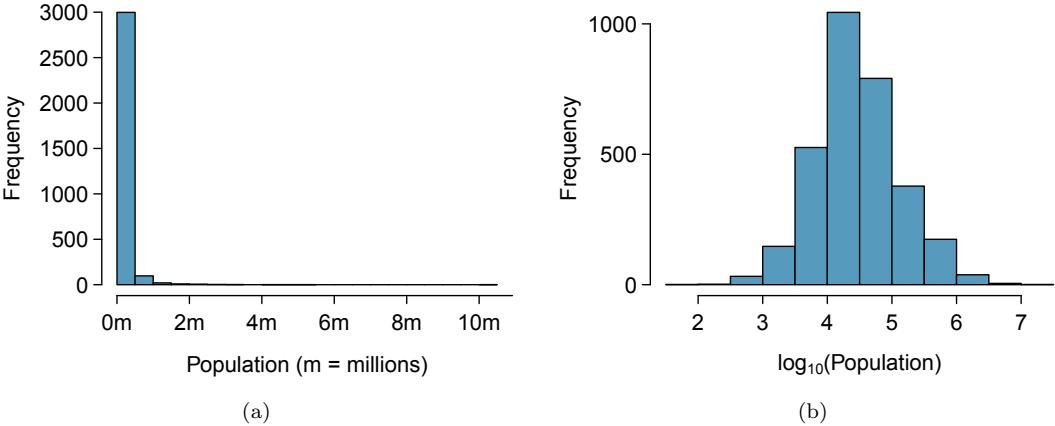
\includegraphics{_page_51_Figure_3.jpeg}

Figura 2.13: \hyperref[page-51-0]{(a)} Un histograma de las poblaciones
de todos los condados de EE. UU. \hyperref[page-51-1]{(b)} Un histograma
de las poblaciones de los condados transformadas con log10. Para este
gráfico, el valor x corresponde a la potencia de 10, p.~ej., ``4'' en el
eje x corresponde a 104 = 10.000.

\paragraph{\texorpdfstring{\textbf{EJEMPLO
2.20}}{EJEMPLO 2.20}}\label{ejemplo-2.20}

Considere el histograma de las poblaciones de los condados que se
muestra en la Figura \hyperref[page-51-0]{2.13(a),} que muestra una
asimetría extrema. ¿Qué no es útil de este gráfico?

Casi todos los datos caen en el bin más a la izquierda, y la asimetría
extrema oscurece muchos de los detalles potencialmente interesantes de
los datos.

Existen algunas transformaciones estándar que pueden ser útiles para
datos fuertemente sesgados a la derecha donde gran parte de los datos
son positivos pero están agrupados cerca de cero. Una transformación es
un reescalado de los datos utilizando una función. Por ejemplo, un
gráfico del logaritmo (base 10) de las poblaciones de los condados da
como resultado el nuevo histograma en la Figura
\hyperref[page-51-1]{2.13(b).} Estos datos son simétricos y cualquier
valor atípico potencial parece mucho menos extremo que en el conjunto de
datos original. Al controlar los valores atípicos y la asimetría
extrema, las transformaciones como esta a menudo facilitan la
construcción de modelos estadísticos contra los datos.

Las transformaciones también se pueden aplicar a una o ambas variables
en un diagrama de dispersión. Un diagrama de dispersión del cambio de
población de 2010 a 2017 frente a la población en 2010 se muestra en la
Figura \hyperref[page-52-0]{2.14(a).} En este primer diagrama de
dispersión, es difícil descifrar patrones interesantes porque la
variable de población está muy sesgada. Sin embargo, si aplicamos una
transformación log10 a la variable de población, como se muestra en la
Figura \hyperref[page-52-1]{2.14(b),} se revela una asociación positiva
entre las variables. De hecho, es posible que estemos interesados
\hspace{0pt}\hspace{0pt}en ajustar una línea de tendencia a los datos
cuando exploremos métodos para ajustar líneas de regresión en el
Capítulo \hyperref[page-302-0]{8.}

Otras transformaciones además del logaritmo también pueden ser útiles.
Por ejemplo, la raíz cuadrada ( √ observación original) y la inversa ( 1
observación original) son comúnmente utilizadas por los científicos de
datos. Los objetivos comunes al transformar datos son ver la estructura
de los datos de manera diferente, reducir la asimetría, ayudar en el
modelado o enderezar una relación no lineal en un diagrama de
dispersión.

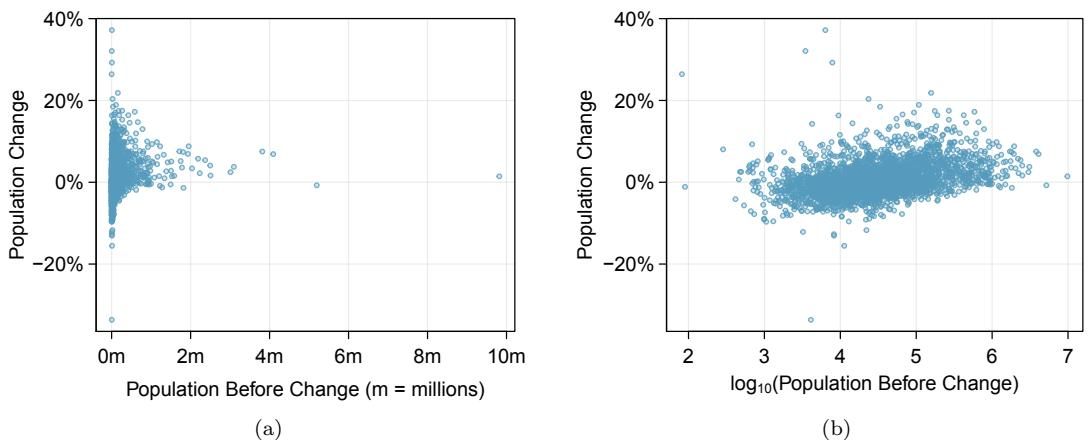
\includegraphics{_page_52_Figure_1.jpeg}

Figura 2.14: \hyperref[page-52-0]{(a)} Diagrama de dispersión del cambio
de población frente a la población antes del cambio.
\hyperref[page-52-1]{(b)} Un diagrama de dispersión de los mismos datos,
pero donde el tamaño de la población se ha transformado
logarítmicamente.

\section{\texorpdfstring{\textbf{2.1.8 Mapeo de datos (tema
especial)}}{2.1.8 Mapeo de datos (tema especial)}}\label{mapeo-de-datos-tema-especial}

El conjunto de datos del condado ofrece muchas variables numéricas que
podríamos graficar usando diagramas de puntos, diagramas de dispersión o
diagramas de caja, pero estos no capturan la verdadera naturaleza de los
datos. Más bien, cuando encontramos datos geográficos, debemos crear un
mapa de intensidad, donde los colores se utilizan para mostrar valores
más altos y más bajos de una variable. Las figuras
\hyperref[page-53-0]{2.15} y \hyperref[page-54-0]{2.16} muestran mapas
de intensidad para la tasa de pobreza en porcentaje (pobreza), la tasa
de desempleo (tasa de desempleo), la tasa de propiedad de vivienda en
porcentaje (propiedad de vivienda) y el ingreso medio por hogar (ingreso
medio por hogar). La clave de color indica qué colores corresponden a
qué valores. Los mapas de intensidad generalmente no son muy útiles para
obtener valores precisos en un condado determinado, pero son muy útiles
para ver tendencias geográficas y generar preguntas o hipótesis de
investigación interesantes.

\subsection{\texorpdfstring{\textbf{EJEMPLO
2.21}}{EJEMPLO 2.21}}\label{ejemplo-2.21}

¿Qué características interesantes son evidentes en los mapas de
intensidad de la pobreza y la tasa de desempleo?

Las tasas de pobreza son evidentemente más altas en algunos lugares. En
particular, el sur profundo muestra tasas de pobreza más altas, al igual
que gran parte de Arizona y Nuevo México. Las altas tasas de pobreza son
evidentes en las llanuras aluviales de Mississippi, un poco al norte de
Nueva Orleans, y también en una gran sección de Kentucky.

La tasa de desempleo sigue tendencias similares, y podemos ver
correspondencia entre las dos variables. De hecho, tiene sentido que las
tasas más altas de desempleo estén estrechamente relacionadas con las
tasas de pobreza. Una observación que destaca al comparar los dos mapas:
la tasa de pobreza es mucho más alta que la tasa de desempleo, lo que
significa que, aunque muchas personas pueden estar trabajando, no están
ganando lo suficiente para salir de la pobreza.

\subsection{\texorpdfstring{\textbf{PRÁCTICA GUIADA
2.22}}{PRÁCTICA GUIADA 2.22}}\label{pruxe1ctica-guiada-2.22}

¿Qué características interesantes son evidentes en el mapa de intensidad
del ingreso medio por hogar en la Figura \hyperref[page-54-1]{2.16(b)?}
\hyperref[page-52-2]{14}

14Nota: las respuestas variarán. Existe cierta correspondencia entre las
zonas de altos ingresos y las zonas metropolitanas, donde podemos ver
puntos más oscuros (mayor ingreso medio por hogar), aunque hay varias
excepciones. Puede buscar grandes ciudades con las que esté
familiarizado e intentar localizarlas en el mapa como puntos oscuros.

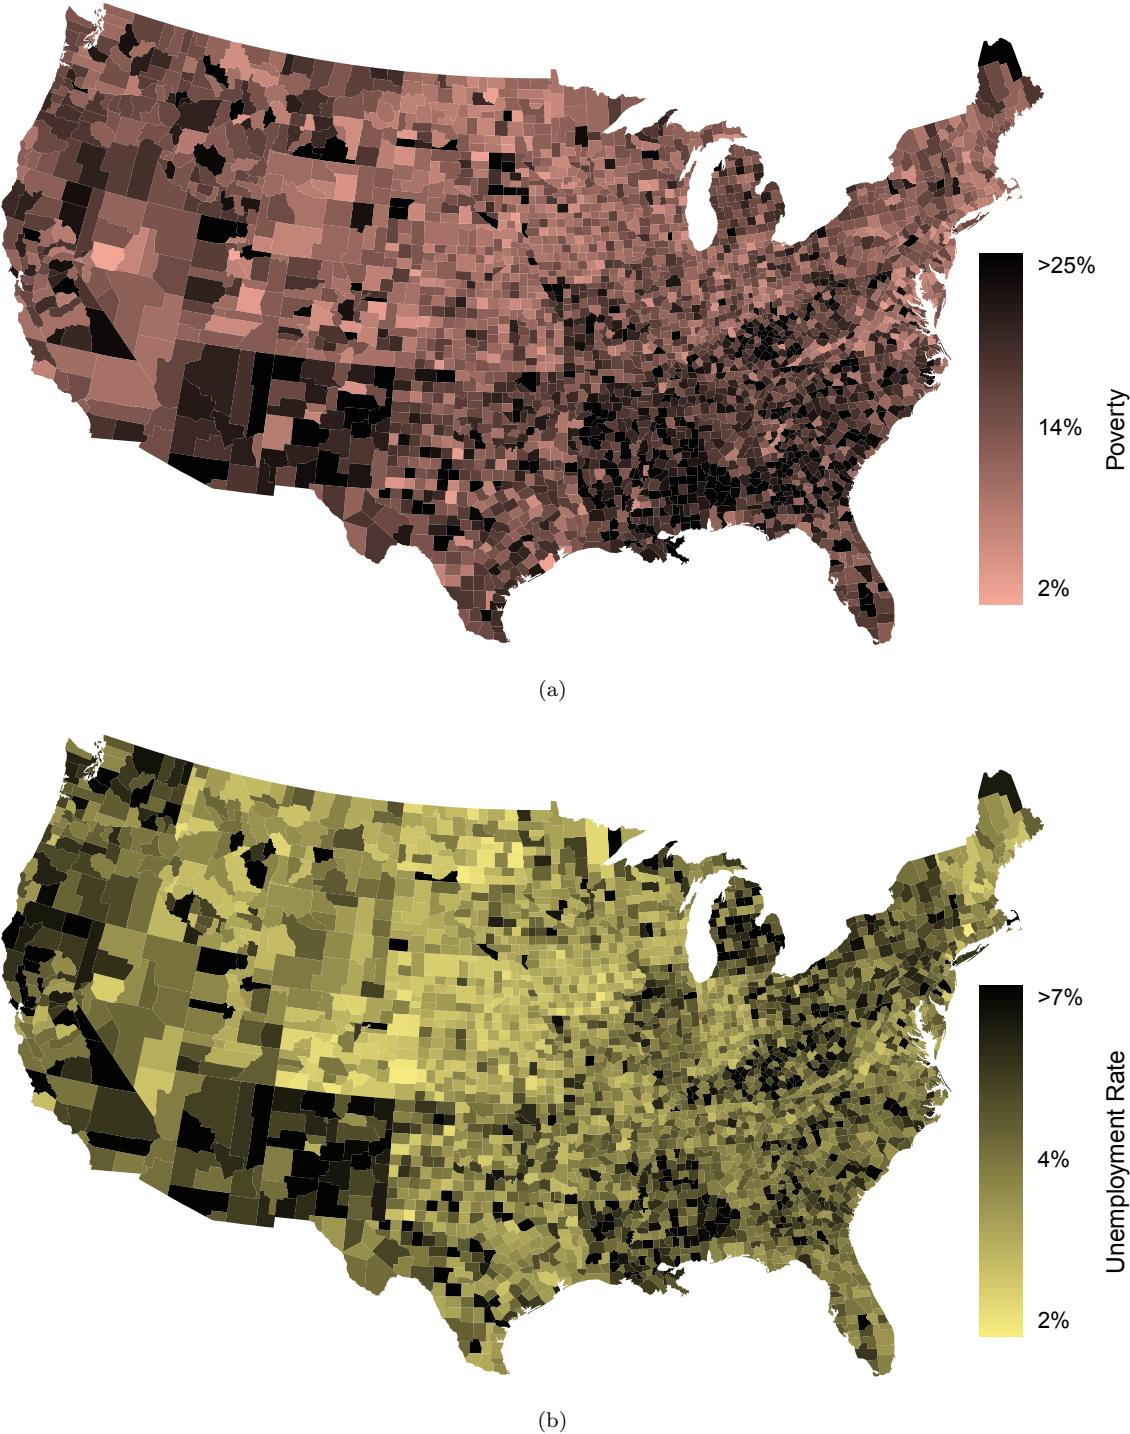
\includegraphics{_page_53_Picture_1.jpeg}

Figura 2.15: \hyperref[page-53-1]{(a)} Mapa de intensidad de la tasa de
pobreza (porcentaje). \hyperref[page-53-2]{(b)} Mapa de la tasa de
desempleo (porcentaje).

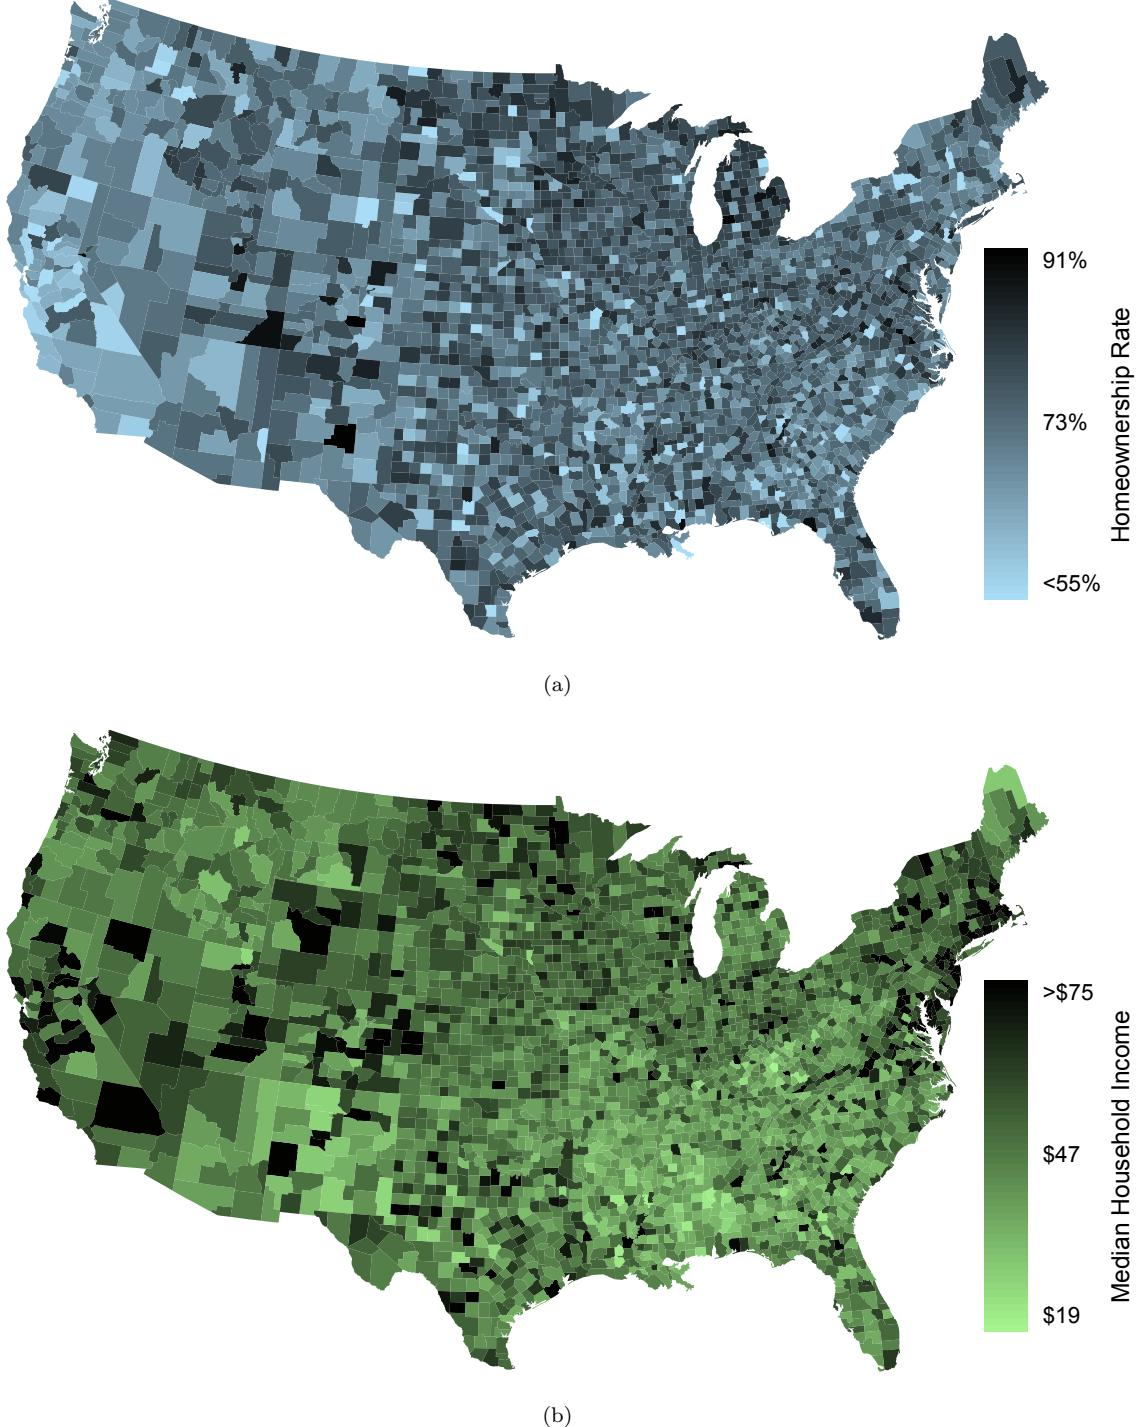
\includegraphics{_page_54_Figure_1.jpeg}

Figura 2.16: \hyperref[page-54-2]{(a)} Mapa de intensidad de la tasa de
propiedad de vivienda (porcentaje). \hyperref[page-54-1]{(b)} Mapa de
intensidad del ingreso medio por hogar (\$1000s).

\section{\texorpdfstring{\textbf{Ejercicios}}{Ejercicios}}\label{ejercicios-2}

\hyperref[page-384-20]{\textbf{2.1}} \textbf{Esperanza de vida de
mamíferos.} Se recolectaron datos sobre la esperanza de vida (en años) y
la duración de la gestación (en días) de 62 mamíferos. A continuación,
se muestra un diagrama de dispersión de la esperanza de vida frente a la
duración de la gestación.\hyperref[page-55-0]{15}

\begin{itemize}
\tightlist
\item
  \begin{enumerate}
  \def\labelenumi{(\alph{enumi})}
  \tightlist
  \item
    ¿Qué tipo de asociación es evidente entre la esperanza de vida y la
    duración de la gestación?
  \end{enumerate}
\item
  \begin{enumerate}
  \def\labelenumi{(\alph{enumi})}
  \setcounter{enumi}{1}
  \tightlist
  \item
    ¿Qué tipo de asociación esperaría ver si se invirtieran los ejes del
    gráfico, es decir, si graficáramos la duración de la gestación
    frente a la esperanza de vida?
  \end{enumerate}
\item
  \begin{enumerate}
  \def\labelenumi{(\alph{enumi})}
  \setcounter{enumi}{2}
  \tightlist
  \item
    ¿Son independientes la esperanza de vida y la duración de la
    gestación? Explique su razonamiento.
  \end{enumerate}
\end{itemize}

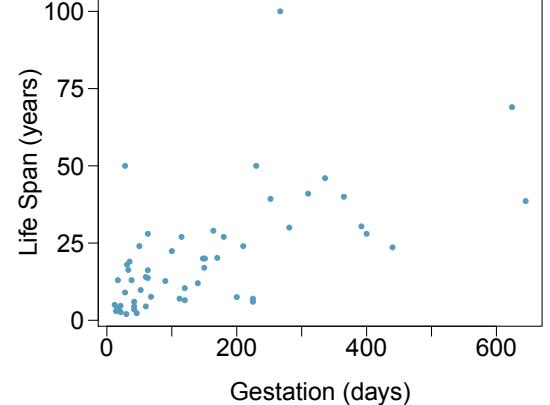
\includegraphics{_page_55_Figure_6.jpeg}

\hyperref[page-384-21]{\textbf{2.2}} \textbf{Asociaciones.} Indique
cuáles de los gráficos muestran (a) una asociación positiva, (b) una
asociación negativa o (c) ninguna asociación. Determine también si las
asociaciones positivas y negativas son lineales o no lineales. Cada
parte puede referirse a más de un gráfico.

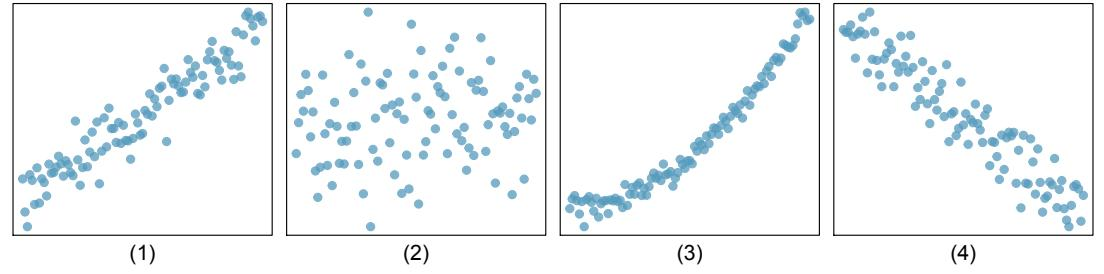
\includegraphics{_page_55_Figure_8.jpeg}

\hyperref[page-384-22]{\textbf{2.3}} \textbf{Reproducción de bacterias.}
Suponga que solo hay suficiente espacio y nutrientes para mantener un
millón de células bacterianas en una placa de Petri. Coloca algunas
células bacterianas en esta placa de Petri, permite que se reproduzcan
libremente y registra el número de células bacterianas en la placa a lo
largo del tiempo. Dibuje un gráfico que represente la relación entre el
número de células bacterianas y el tiempo.

\hyperref[page-384-23]{\textbf{2.4}} \textbf{Productividad de la
oficina.} La productividad de la oficina es relativamente baja cuando
los empleados no sienten estrés por su trabajo o seguridad laboral. Sin
embargo, los altos niveles de estrés también pueden conducir a una
reducción de la productividad de los empleados. Dibuje un gráfico para
representar la relación entre el estrés y la productividad.

\hyperref[page-384-24]{\textbf{2.5}} \textbf{Parámetros y estadísticas.}
Identifique qué valor representa la media muestral y qué valor
representa la media poblacional reclamada.

\begin{itemize}
\tightlist
\item
  \begin{enumerate}
  \def\labelenumi{(\alph{enumi})}
  \tightlist
  \item
    Los hogares estadounidenses gastaron un promedio de aproximadamente
    \$52 en 2007 en productos de Halloween, como disfraces, adornos y
    dulces. Para ver si este número había cambiado, los investigadores
    realizaron una nueva encuesta en 2008 antes de que se informaran los
    números de la industria. La encuesta incluyó a 1,500 hogares y
    encontró que el gasto promedio en Halloween fue de \$58 por hogar.
  \end{enumerate}
\item
  \begin{enumerate}
  \def\labelenumi{(\alph{enumi})}
  \setcounter{enumi}{1}
  \tightlist
  \item
    El GPA promedio de los estudiantes en 2001 en una universidad
    privada fue de 3.37. Una encuesta en una muestra de 203 estudiantes
    de esta universidad arrojó un GPA promedio de 3.59 una década
    después.
  \end{enumerate}
\end{itemize}

\hyperref[page-384-25]{\textbf{2.6}} \textbf{Dormir en la universidad.}
Un artículo reciente en un periódico universitario decía que los
estudiantes universitarios duermen un promedio de 5.5 horas cada noche.
Un estudiante que se mostraba escéptico sobre este valor decidió
realizar una encuesta muestreando aleatoriamente a 25 estudiantes. En
promedio, los estudiantes muestreados durmieron 6.25 horas por noche.
Identifique qué valor representa la media muestral y qué valor
representa la media poblacional reclamada.

15T. Allison y D.V. Cicchetti.
\href{http://www.openintro.org/redirect.php?go=textbook-mammal_sleep_1975&referrer=os4_pdf}{``Sleep
in mammals: ecological and constitutional correlates''}. In: Arch.
Hydrobiol 75 (1975), p.~442.

\section{2.1. EXAMINANDO DATOS NUMÉRICOS
57}\label{examinando-datos-numuxe9ricos-57}

\hyperref[page-384-26]{\textbf{2.7}} \textbf{Días libres en una planta
minera.} Los trabajadores de un sitio minero en particular reciben un
promedio de 35 días de vacaciones pagadas, lo cual es inferior al
promedio nacional. El gerente de esta planta está bajo presión de un
sindicato local para aumentar la cantidad de tiempo libre pagado. Sin
embargo, no quiere dar más días libres a los trabajadores porque eso
sería costoso. En cambio, decide que debería despedir a 10 empleados de
tal manera que aumente el número promedio de días libres que informan
sus empleados. Para lograr este objetivo, ¿debería despedir a los
empleados que tienen la mayor cantidad de días libres, la menor cantidad
de días libres o aquellos que tienen aproximadamente el número promedio
de días libres?

\hyperref[page-384-27]{\textbf{2.8}} \textbf{Medianas y RICs.} Para cada
parte, compare las distribuciones (1) y (2) según sus medianas y RICs.
No es necesario que calcule estas estadísticas; simplemente indique cómo
se comparan las medianas y los RICs. Asegúrese de explicar su
razonamiento.

\begin{longtable}[]{@{}
  >{\raggedright\arraybackslash}p{(\columnwidth - 4\tabcolsep) * \real{0.3247}}
  >{\raggedright\arraybackslash}p{(\columnwidth - 4\tabcolsep) * \real{0.2857}}
  >{\raggedright\arraybackslash}p{(\columnwidth - 4\tabcolsep) * \real{0.3896}}@{}}
\toprule\noalign{}
\begin{minipage}[b]{\linewidth}\raggedright
(a) (1) 3, 5, 6, 7, 9
\end{minipage} & \begin{minipage}[b]{\linewidth}\raggedright
\end{minipage} & \begin{minipage}[b]{\linewidth}\raggedright
(c) (1) 1, 2, 3, 4, 5
\end{minipage} \\
\midrule\noalign{}
\endhead
\bottomrule\noalign{}
\endlastfoot
& (2) 3, 5, 6, 7, 20 & (2) 6, 7, 8, 9, 10 \\
(b) (1) 3, 5, 6, 7, 9 & & (d) (1) 0, 10, 50, 60, 100 \\
& (2) 3, 5, 7, 8, 9 & (2) 0, 100, 500, 600, 1000 \\
\end{longtable}

\hyperref[page-385-0]{\textbf{2.9}} \textbf{Medias y DEs.} Para cada
parte, compare las distribuciones (1) y (2) según sus medias y
desviaciones estándar. No es necesario que calcule estas estadísticas;
simplemente indique cómo se comparan las medias y las desviaciones
estándar. Asegúrese de explicar su razonamiento. Sugerencia: Puede ser
útil dibujar diagramas de puntos de las distribuciones.

\begin{longtable}[]{@{}
  >{\raggedright\arraybackslash}p{(\columnwidth - 2\tabcolsep) * \real{0.5000}}
  >{\raggedright\arraybackslash}p{(\columnwidth - 2\tabcolsep) * \real{0.5000}}@{}}
\toprule\noalign{}
\begin{minipage}[b]{\linewidth}\raggedright
(a) (1) 3, 5, 5, 5, 8, 11, 11, 11, 13(2) 3, 5, 5, 5, 8, 11, 11, 11, 20
\end{minipage} & \begin{minipage}[b]{\linewidth}\raggedright
(c) (1) 0, 2, 4, 6, 8, 10(2) 20, 22, 24, 26, 28, 30
\end{minipage} \\
\midrule\noalign{}
\endhead
\bottomrule\noalign{}
\endlastfoot
(b) (1) -20, 0, 0, 0, 15, 25, 30, 30(2) -40, 0, 0, 0, 15, 25, 30, 30 &
(d) (1) 100, 200, 300, 400, 500(2) 0, 50, 300, 550, 600 \\
\end{longtable}

\hyperref[page-385-1]{\textbf{2.10}} \textbf{Mezclar y combinar.}
Describe la distribución en los histogramas a continuación y haz
coincidir con los diagramas de caja.

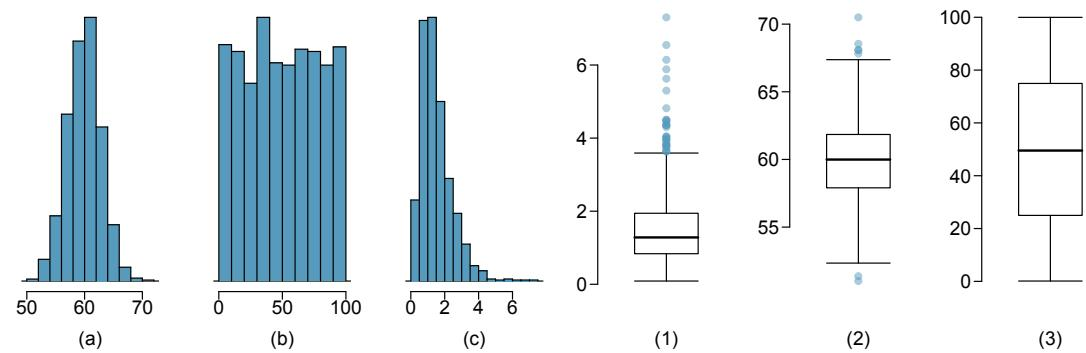
\includegraphics{_page_56_Figure_7.jpeg}

\hyperref[page-385-2]{\textbf{2.11}} \textbf{Calidad del aire.} La
calidad del aire diaria se mide mediante el índice de calidad del aire
(ICA) informado por la Agencia de Protección Ambiental. Este índice
informa el nivel de contaminación y qué efectos asociados en la salud
podrían ser una preocupación. El índice se calcula para cinco
contaminantes principales del aire regulados por la Ley de Aire Limpio y
toma valores de 0 a 300, donde un valor más alto indica una menor
calidad del aire. El ICA se informó para una muestra de 91 días en 2011
en Durham, NC.\hyperref[page-57-0]{16}

\begin{itemize}
\tightlist
\item
  \begin{enumerate}
  \def\labelenumi{(\alph{enumi})}
  \tightlist
  \item
    Estima el valor mediano del ICA de esta muestra.
  \end{enumerate}
\item
  \begin{enumerate}
  \def\labelenumi{(\alph{enumi})}
  \setcounter{enumi}{1}
  \tightlist
  \item
    ¿Esperaría que el valor medio del ICA de esta muestra sea mayor o
    menor que la mediana? Explica tu razonamiento.
  \end{enumerate}
\item
  \begin{enumerate}
  \def\labelenumi{(\alph{enumi})}
  \setcounter{enumi}{2}
  \tightlist
  \item
    Estima Q1, Q3 e IQR para la distribución.
  \end{enumerate}
\item
  \begin{enumerate}
  \def\labelenumi{(\alph{enumi})}
  \setcounter{enumi}{3}
  \tightlist
  \item
    ¿Alguno de los días de esta muestra se consideraría que tiene un ICA
    inusualmente bajo o alto? Explica tu razonamiento.
  \end{enumerate}
\end{itemize}

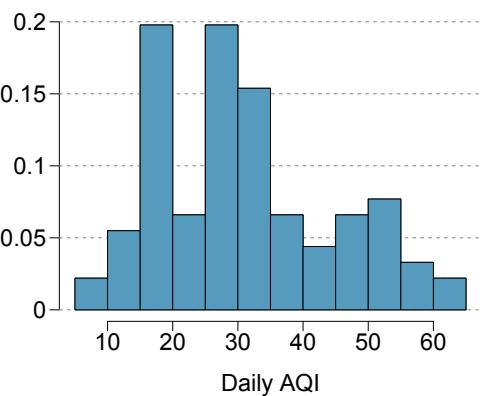
\includegraphics{_page_57_Figure_6.jpeg}

\hyperref[page-385-3]{\textbf{2.12}} \textbf{Mediana vs.~media.} Estima
la mediana para las 400 observaciones que se muestran en el histograma y
ten en cuenta si esperas que la media sea mayor o menor que la mediana.

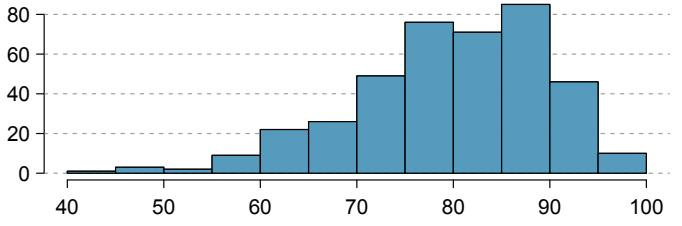
\includegraphics{_page_57_Figure_8.jpeg}

\hyperref[page-385-4]{\textbf{2.13}} \textbf{Histogramas vs.~diagramas
de caja.} Compare los dos diagramas a continuación. ¿Qué características
de la distribución son evidentes en el histograma y no en el diagrama de
caja? ¿Qué características son evidentes en el diagrama de caja pero no
en el histograma?

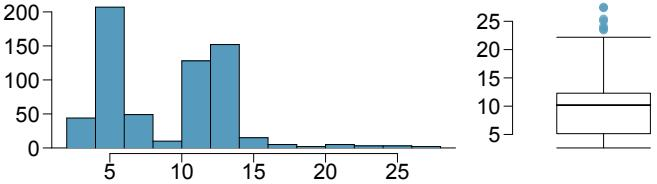
\includegraphics{_page_57_Figure_10.jpeg}

\hyperref[page-385-5]{\textbf{2.14}} \textbf{Amigos de Facebook.} Los
datos de Facebook indican que el 50\% de los usuarios de Facebook tienen
100 o más amigos, y que el número promedio de amigos de los usuarios es
de 190. ¿Qué sugieren estos hallazgos sobre la forma de la distribución
del número de amigos de los usuarios de
Facebook?\hyperref[page-57-1]{17}

\hyperref[page-385-6]{\textbf{2.15}} \textbf{Distribuciones y
estadísticas apropiadas, Parte I.} Para cada uno de los siguientes,
indica si esperas que la distribución sea simétrica, sesgada a la
derecha o sesgada a la izquierda. Especifica también si la media o la
mediana representarían mejor una observación típica en los datos, y si
la variabilidad de las observaciones estaría mejor representada usando
la desviación estándar o el IQR. Explica tu razonamiento.

\begin{itemize}
\tightlist
\item
  \begin{enumerate}
  \def\labelenumi{(\alph{enumi})}
  \tightlist
  \item
    Número de mascotas por hogar.
  \end{enumerate}
\item
  \begin{enumerate}
  \def\labelenumi{(\alph{enumi})}
  \setcounter{enumi}{1}
  \tightlist
  \item
    Distancia al trabajo, es decir, número de millas entre el trabajo y
    el hogar.
  \end{enumerate}
\item
  \begin{enumerate}
  \def\labelenumi{(\alph{enumi})}
  \setcounter{enumi}{2}
  \tightlist
  \item
    Alturas de hombres adultos.
  \end{enumerate}
\end{itemize}

16Agencia de Protección Ambiental de EE. UU.,
\href{http://www.openintro.org/redirect.php?go=textbook-airdata_2011&referrer=os4_pdf}{AirData,
2011.}

17Lars Backstrom.
\href{http://www.openintro.org/redirect.php?go=textbook-anatomy-of-facebook&referrer=os4_pdf}{``Anatomía
de Facebook''}. En: Notas del equipo de datos de Facebook (2011).

\hyperref[page-385-7]{\textbf{2.16}} \textbf{Distribuciones y
estadísticas apropiadas, Parte II.} Para cada uno de los siguientes,
indica si esperas que la distribución sea simétrica, sesgada a la
derecha o sesgada a la izquierda. Especifica también si la media o la
mediana representarían mejor una observación típica en los datos, y si
la variabilidad de las observaciones estaría mejor representada usando
la desviación estándar o el IQR. Explica tu razonamiento.

\begin{itemize}
\tightlist
\item
  \begin{enumerate}
  \def\labelenumi{(\alph{enumi})}
  \tightlist
  \item
    Precios de la vivienda en un país donde el 25\% de las casas cuestan
    menos de \$350,000, el 50\% de las casas cuestan menos de \$450,000,
    el 75\% de las casas cuestan menos de \$1,000,000 y hay un número
    significativo de casas que cuestan más de \$6,000,000.
  \end{enumerate}
\item
  \begin{enumerate}
  \def\labelenumi{(\alph{enumi})}
  \setcounter{enumi}{1}
  \tightlist
  \item
    Precios de la vivienda en un país donde el 25\% de las casas cuestan
    menos de \$300,000, el 50\% de las casas cuestan menos de \$600,000,
    el 75\% de las casas cuestan menos de \$900,000 y muy pocas casas
    cuestan más de \$1,200,000.
  \end{enumerate}
\item
  \begin{enumerate}
  \def\labelenumi{(\alph{enumi})}
  \setcounter{enumi}{2}
  \tightlist
  \item
    Número de bebidas alcohólicas consumidas por estudiantes
    universitarios en una semana determinada. Suponga que la mayoría de
    estos estudiantes no beben porque son menores de 21 años, y solo
    unos pocos beben en exceso.
  \end{enumerate}
\item
  \begin{enumerate}
  \def\labelenumi{(\alph{enumi})}
  \setcounter{enumi}{3}
  \tightlist
  \item
    Salarios anuales de los empleados de una empresa Fortune 500 donde
    solo unos pocos ejecutivos de alto nivel ganan salarios mucho más
    altos que todos los demás empleados.
  \end{enumerate}
\end{itemize}

\hyperref[page-385-8]{\textbf{2.17}} \textbf{Ingresos en la cafetería.}
El primer histograma a continuación muestra la distribución de los
ingresos anuales de 40 clientes en una cafetería universitaria. Suponga
que dos nuevas personas entran en la cafetería: una que gana \$225,000 y
la otra \$250,000. El segundo histograma muestra la nueva distribución
de ingresos. También se proporcionan estadísticas resumidas.

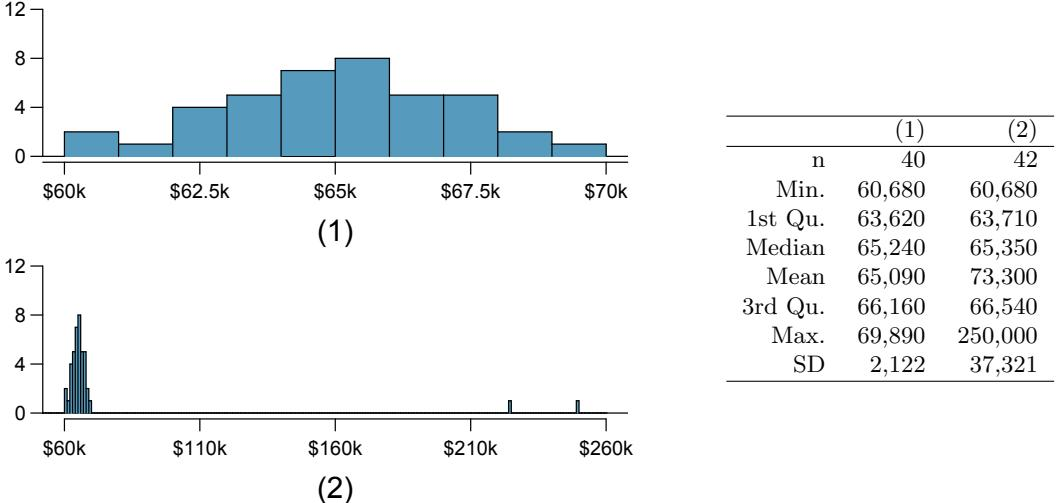
\includegraphics{_page_58_Figure_7.jpeg}

(a) ¿La media o la mediana representarían mejor lo que podríamos
considerar un ingreso típico para los 42 clientes de esta cafetería?
¿Qué dice esto sobre la robustez de las dos medidas?

\begin{enumerate}
\def\labelenumi{(\alph{enumi})}
\setcounter{enumi}{1}
\tightlist
\item
  ¿La desviación estándar o el IQR representarían mejor la cantidad de
  variabilidad en los ingresos de los 42 clientes de esta cafetería?
  ¿Qué dice esto sobre la robustez de las dos medidas?
\end{enumerate}

\hyperref[page-385-9]{\textbf{2.18}} \textbf{Rango medio.} El rango
medio de una distribución se define como el promedio del máximo y el
mínimo de esa distribución. ¿Es esta estadística robusta a los valores
atípicos y al sesgo extremo? Explica tu razonamiento.

\hyperref[page-385-10]{\textbf{2.19}} \textbf{Tiempos de viaje.} El
censo de EE. UU. recopila datos sobre el tiempo que tardan los
estadounidenses en viajar al trabajo, entre muchas otras variables. El
histograma a continuación muestra la distribución de los tiempos
promedio de viaje en 3,142 condados de EE. UU. en 2010. También se
muestra a continuación un mapa de intensidad espacial de los mismos
datos.

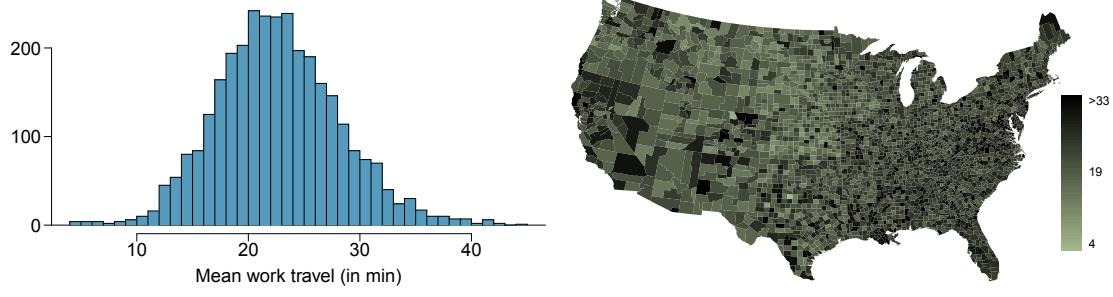
\includegraphics{_page_59_Figure_2.jpeg}

\begin{itemize}
\tightlist
\item
  \begin{enumerate}
  \def\labelenumi{(\alph{enumi})}
  \tightlist
  \item
    Describe la distribución numérica y comenta si una transformación
    logarítmica podría ser aconsejable para estos datos.
  \end{enumerate}
\item
  \begin{enumerate}
  \def\labelenumi{(\alph{enumi})}
  \setcounter{enumi}{1}
  \tightlist
  \item
    Describe la distribución espacial de los tiempos de viaje utilizando
    el mapa anterior.
  \end{enumerate}
\end{itemize}

\hyperref[page-385-11]{\textbf{2.20}} \textbf{Población hispana.} El
censo de EE. UU. recopila datos sobre la raza y el origen étnico de los
estadounidenses, entre muchas otras variables. El histograma a
continuación muestra la distribución del porcentaje de la población que
es hispana en 3,142 condados de los EE. UU. en 2010. También se muestra
un histograma de los logaritmos de estos valores.

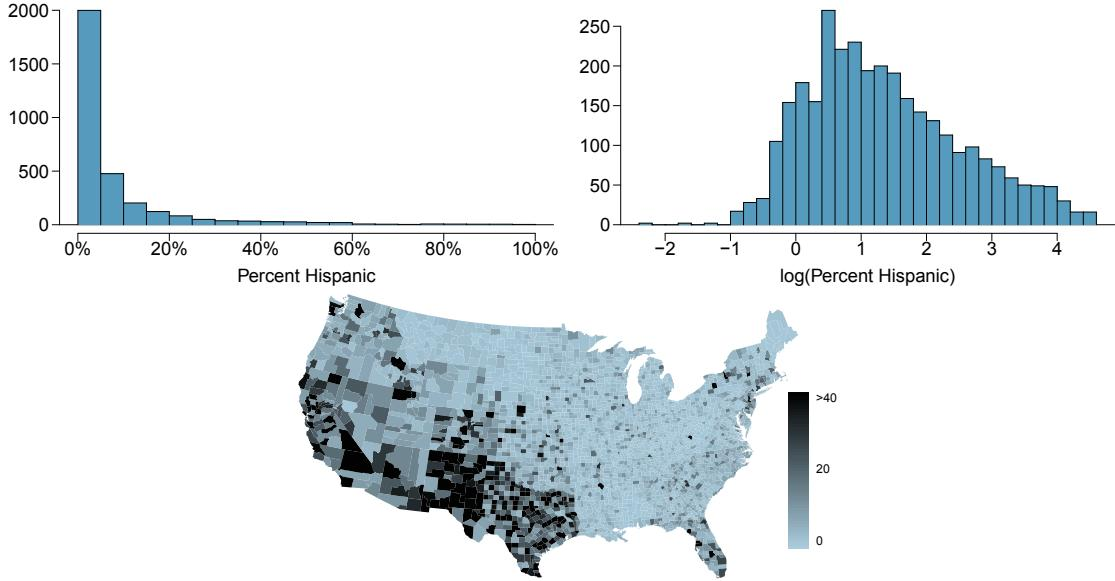
\includegraphics{_page_59_Figure_6.jpeg}

\begin{itemize}
\tightlist
\item
  \begin{enumerate}
  \def\labelenumi{(\alph{enumi})}
  \tightlist
  \item
    Describe la distribución numérica y comenta por qué podríamos querer
    usar valores transformados logarítmicamente al analizar o modelar
    estos datos.
  \end{enumerate}
\item
  \begin{enumerate}
  \def\labelenumi{(\alph{enumi})}
  \setcounter{enumi}{1}
  \tightlist
  \item
    ¿Qué características de la distribución de la población hispana en
    los condados de EE. UU. son evidentes en el mapa pero no en el
    histograma? ¿Qué características son evidentes en el histograma pero
    no en el mapa?
  \end{enumerate}
\item
  \begin{enumerate}
  \def\labelenumi{(\alph{enumi})}
  \setcounter{enumi}{2}
  \tightlist
  \item
    ¿Es una visualización más apropiada o útil que la otra? Explica tu
    razonamiento.
  \end{enumerate}
\end{itemize}

\section{\texorpdfstring{\textbf{2.2 Considerando datos
categóricos}}{2.2 Considerando datos categóricos}}\label{considerando-datos-categuxf3ricos}

En esta sección, presentaremos tablas y otras herramientas básicas para
datos categóricos que se utilizan en todo este libro. El conjunto de
datos loan50 representa una muestra de un conjunto de datos de préstamos
más grande llamado loans. Este conjunto de datos más grande contiene
información sobre 10,000 préstamos realizados a través de Lending Club.
Examinaremos la relación entre la propiedad de la vivienda, que para los
datos de los préstamos puede tomar un valor de alquiler, hipoteca (posee
pero tiene una hipoteca) o propia, y el tipo de aplicación, que indica
si la solicitud de préstamo se realizó con un socio o si era una
solicitud individual.

\section{\texorpdfstring{\textbf{2.2.1 Tablas de contingencia y
diagramas de
barras}}{2.2.1 Tablas de contingencia y diagramas de barras}}\label{tablas-de-contingencia-y-diagramas-de-barras}

La Figura \hyperref[page-60-1]{2.17} resume dos variables: tipo de
solicitud y tenencia de vivienda. Una tabla que resume datos para dos
variables categóricas de esta manera se llama tabla de contingencia.
Cada valor en la tabla representa el número de veces que ocurrió una
combinación particular de resultados de variables. Por ejemplo, el valor
3496 corresponde al número de préstamos en el conjunto de datos donde el
prestatario alquila su vivienda y el tipo de solicitud fue individual.
También se incluyen los totales de filas y columnas. Los totales de
filas proporcionan los conteos totales en cada fila (p.~ej., 3496 + 3839
+ 1170 = 8505), y los totales de columnas son los conteos totales en
cada columna. También podemos crear una tabla que muestre solo los
porcentajes o proporciones generales para cada combinación de
categorías, o podemos crear una tabla para una sola variable, como la
que se muestra en la Figura \hyperref[page-60-2]{2.18} para la variable
de tenencia de vivienda.

\begin{longtable}[]{@{}
  >{\raggedright\arraybackslash}p{(\columnwidth - 10\tabcolsep) * \real{0.1571}}
  >{\raggedright\arraybackslash}p{(\columnwidth - 10\tabcolsep) * \real{0.1714}}
  >{\raggedright\arraybackslash}p{(\columnwidth - 10\tabcolsep) * \real{0.3143}}
  >{\raggedright\arraybackslash}p{(\columnwidth - 10\tabcolsep) * \real{0.1429}}
  >{\raggedright\arraybackslash}p{(\columnwidth - 10\tabcolsep) * \real{0.1143}}
  >{\raggedright\arraybackslash}p{(\columnwidth - 10\tabcolsep) * \real{0.1000}}@{}}
\toprule\noalign{}
\begin{minipage}[b]{\linewidth}\raggedright
\end{minipage} & \begin{minipage}[b]{\linewidth}\raggedright
\end{minipage} & \begin{minipage}[b]{\linewidth}\raggedright
Tenencia de Vivienda
\end{minipage} & \begin{minipage}[b]{\linewidth}\raggedright
\end{minipage} & \begin{minipage}[b]{\linewidth}\raggedright
\end{minipage} & \begin{minipage}[b]{\linewidth}\raggedright
\end{minipage} \\
\midrule\noalign{}
\endhead
\bottomrule\noalign{}
\endlastfoot
& & alquiler & hipoteca & propia & Total \\
& individual & 3496 & 3839 & 1170 & 8505 \\
Tipo Sol. & conjunta & 362 & 950 & 183 & 1495 \\
& Total & 3858 & 4789 & 1353 & 10000 \\
\end{longtable}

\begin{longtable}[]{@{}ll@{}}
\toprule\noalign{}
Tenencia de Vivienda & Conteo \\
\midrule\noalign{}
\endhead
\bottomrule\noalign{}
\endlastfoot
alquiler & 3858 \\
hipoteca & 4789 \\
propia & 1353 \\
Total & 10000 \\
\end{longtable}

Figura 2.17: Una tabla de contingencia para el tipo de solicitud y la
tenencia de vivienda.

Figura 2.18: Una tabla que resume las frecuencias de cada valor para la
variable de tenencia de vivienda.

Un diagrama de barras es una forma común de mostrar una sola variable
categórica. El panel izquierdo de la Figura \hyperref[page-61-0]{2.19}
muestra un diagrama de barras para la variable de tenencia de vivienda.
En el panel derecho, los conteos se convierten en proporciones,
mostrando la proporción de observaciones que se encuentran en cada nivel
(p.~ej., 3858/10000 = 0.3858 para alquiler).

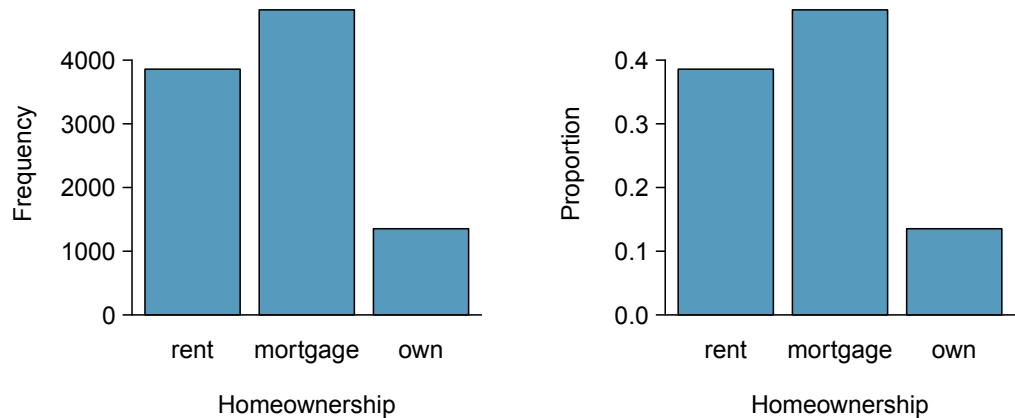
\includegraphics{_page_61_Figure_1.jpeg}

Figura 2.19: Dos diagramas de barras de número. El panel izquierdo
muestra los conteos y el panel derecho muestra las proporciones en cada
grupo.

\section{\texorpdfstring{\textbf{2.2.2 Proporciones de fila y
columna}}{2.2.2 Proporciones de fila y columna}}\label{proporciones-de-fila-y-columna}

A veces es útil comprender la descomposición fraccionaria de una
variable en otra, y podemos modificar nuestra tabla de contingencia para
proporcionar tal vista. La Figura \hyperref[page-61-1]{2.20} muestra las
proporciones de fila para la Figura \hyperref[page-60-1]{2.17,} que se
calculan como los recuentos divididos por sus totales de fila. El valor
3496 en la intersección de individual y alquiler se reemplaza por
3496/8505 = 0.411, es decir, 3496 dividido por su total de fila, 8505.
Entonces, ¿qué representa 0.411? Corresponde a la proporción de
solicitantes individuales que alquilan.

\begin{longtable}[]{@{}lllll@{}}
\toprule\noalign{}
& alquiler & hipoteca & propio & Total \\
\midrule\noalign{}
\endhead
\bottomrule\noalign{}
\endlastfoot
individual & 0.411 & 0.451 & 0.138 & 1.000 \\
conjunta & 0.242 & 0.635 & 0.122 & 1.000 \\
Total & 0.386 & 0.479 & 0.135 & 1.000 \\
\end{longtable}

Figura 2.20: Una tabla de contingencia con proporciones de fila para las
variables de tipo de solicitud y propiedad de la vivienda. El total de
la fila está desviado en 0.001 para la fila conjunta debido a un error
de redondeo.

Una tabla de contingencia de las proporciones de columna se calcula de
manera similar, donde cada proporción de columna se calcula como el
recuento dividido por el total de columna correspondiente. La Figura
\hyperref[page-61-2]{2.21} muestra tal tabla, y aquí el valor 0.906
indica que el 90.6\% de los inquilinos solicitaron el préstamo de forma
individual. Esta tasa es más alta en comparación con los préstamos de
personas con hipotecas (80.2\%) o que son dueños de su casa (86.5\%).
Debido a que estas tasas varían entre los tres niveles de propiedad de
la vivienda (alquiler, hipoteca, propio), esto proporciona evidencia de
que las variables de tipo de solicitud y propiedad de la vivienda están
asociadas.

\begin{longtable}[]{@{}lllll@{}}
\toprule\noalign{}
& alquiler & hipoteca & propio & Total \\
\midrule\noalign{}
\endhead
\bottomrule\noalign{}
\endlastfoot
individual & 0.906 & 0.802 & 0.865 & 0.851 \\
conjunta & 0.094 & 0.198 & 0.135 & 0.150 \\
Total & 1.000 & 1.000 & 1.000 & 1.000 \\
\end{longtable}

Figura 2.21: Una tabla de contingencia con proporciones de columna para
las variables de tipo de solicitud y propiedad de la vivienda. El total
de la última columna está desviado en 0.001 debido a un error de
redondeo.

También podríamos haber verificado una asociación entre el tipo de
solicitud y la propiedad de la vivienda en la Figura
\hyperref[page-61-1]{2.20} utilizando las proporciones de fila. Al
comparar estas proporciones de fila, miraríamos hacia abajo en las
columnas para ver si la fracción de préstamos donde el prestatario
alquila, tiene una hipoteca o es propietario variaba entre los tipos de
solicitud individual y conjunta.

\section{2.2. CONSIDERANDO DATOS CATEGÓRICOS
63}\label{considerando-datos-categuxf3ricos-63}

\section{\texorpdfstring{\textbf{PRÁCTICA GUIADA
2.23}}{PRÁCTICA GUIADA 2.23}}\label{pruxe1ctica-guiada-2.23}

\begin{itemize}
\tightlist
\item
  \begin{enumerate}
  \def\labelenumi{(\alph{enumi})}
  \tightlist
  \item
    ¿Qué representa 0.451 en la Figura \hyperref[page-61-1]{2.20?}
  \end{enumerate}
\item
  \begin{enumerate}
  \def\labelenumi{(\alph{enumi})}
  \setcounter{enumi}{1}
  \tightlist
  \item
    ¿Qué representa 0.802 en la Figura \hyperref[page-61-2]{2.21?}
    \hyperref[page-62-0]{18}
  \end{enumerate}
\end{itemize}

\subsection{\texorpdfstring{\textbf{PRÁCTICA GUIADA
2.24}}{PRÁCTICA GUIADA 2.24}}\label{pruxe1ctica-guiada-2.24}

\begin{itemize}
\tightlist
\item
  \begin{enumerate}
  \def\labelenumi{(\alph{enumi})}
  \tightlist
  \item
    ¿Qué representa 0.122 en la intersección de ``conjunto'' y
    ``propio'' en la Figura \hyperref[page-61-1]{2.20?}
  \end{enumerate}
\item
  \begin{enumerate}
  \def\labelenumi{(\alph{enumi})}
  \setcounter{enumi}{1}
  \tightlist
  \item
    ¿Qué representa 0.135 en la Figura \hyperref[page-61-2]{2.21?}
    \hyperref[page-62-1]{19}
  \end{enumerate}
\end{itemize}

\section{\texorpdfstring{\textbf{EJEMPLO
2.25}}{EJEMPLO 2.25}}\label{ejemplo-2.25}

Los científicos de datos utilizan la estadística para filtrar el spam de
los mensajes de correo electrónico entrantes. Al observar
características específicas de un correo electrónico, un científico de
datos puede clasificar algunos correos electrónicos como spam o no spam
con alta precisión. Una de estas características es si el correo
electrónico no contiene números, números pequeños o números grandes.
Otra característica es el formato del correo electrónico, que indica si
un correo electrónico tiene o no contenido HTML, como texto en negrita.
Nos centraremos en el formato del correo electrónico y el estado de spam
utilizando el conjunto de datos de correo electrónico, y estas variables
se resumen en una tabla de contingencia en la Figura
\hyperref[page-62-2]{2.22.} ¿Qué sería más útil para alguien que espera
clasificar el correo electrónico como spam o correo electrónico normal
para esta tabla: proporciones de fila o de columna?

Un científico de datos estaría interesado en cómo cambia la proporción
de spam dentro de cada formato de correo electrónico. Esto corresponde a
las proporciones de columna: la proporción de spam en los correos
electrónicos de texto sin formato y la proporción de spam en los correos
electrónicos HTML.

Si generamos las proporciones de columna, podemos ver que una mayor
fracción de correos electrónicos de texto sin formato son spam (209/1195
= 17.5\%) en comparación con los correos electrónicos HTML (158/2726 =
5.8\%). Esta información por sí sola es insuficiente para clasificar un
correo electrónico como spam o no spam, ya que más del 80\% de los
correos electrónicos de texto sin formato no son spam. Sin embargo,
cuando combinamos cuidadosamente esta información con muchas otras
características, tenemos una posibilidad razonable de poder clasificar
algunos correos electrónicos como spam o no spam con confianza.

\begin{longtable}[]{@{}llll@{}}
\toprule\noalign{}
& texto & HTML & Total \\
\midrule\noalign{}
\endhead
\bottomrule\noalign{}
\endlastfoot
spam & 209 & 158 & 367 \\
no spam & 986 & 2568 & 3554 \\
Total & 1195 & 2726 & 3921 \\
\end{longtable}

Figura 2.22: Una tabla de contingencia para spam y formato.

El ejemplo \hyperref[page-62-3]{2.25} señala que las proporciones de
fila y columna no son equivalentes. Antes de decidirse por una forma
para una tabla, es importante considerar cada una para asegurarse de que
se construya la tabla más útil. Sin embargo, a veces simplemente no está
claro cuál, si alguna, es más útil.

\subsection{\texorpdfstring{\textbf{EJEMPLO
2.26}}{EJEMPLO 2.26}}\label{ejemplo-2.26}

Vuelva a mirar las Tablas \hyperref[page-61-1]{2.20} y
\hyperref[page-61-2]{2.21.} ¿Hay algún escenario obvio donde uno podría
ser más útil que el otro?

¡Ninguno que pensáramos que fuera obvio! Lo que es distinto sobre el
tipo de aplicación y la propiedad de la vivienda en comparación con el
ejemplo del correo electrónico es que estas dos variables no tienen una
clara relación de variable explicativa-respuesta que podríamos
hipotetizar (vea la Sección \hyperref[page-17-1]{1.2.4} para estos
términos). Por lo general, es más útil ``condicionar'' la variable
explicativa. Por ejemplo, en el ejemplo del correo electrónico, el
formato del correo electrónico se veía como una posible variable
explicativa de si el mensaje era spam, por lo que nos resultaría más
interesante calcular las frecuencias relativas (proporciones) para cada
formato de correo electrónico.

18(a) 0.451 representa la proporción de solicitantes individuales que
tienen una hipoteca. (b) 0.802 representa la fracción de solicitantes
con hipotecas que solicitaron como individuos.

19(a) 0.122 representa la fracción de prestatarios conjuntos que son
dueños de su casa. (b) 0.135 representa los prestatarios propietarios de
viviendas que solicitaron conjuntamente el préstamo.

\section{\texorpdfstring{\textbf{2.2.3 Uso de un diagrama de barras con
dos
variables}}{2.2.3 Uso de un diagrama de barras con dos variables}}\label{uso-de-un-diagrama-de-barras-con-dos-variables}

Las tablas de contingencia que utilizan proporciones de fila o columna
son especialmente útiles para examinar cómo se relacionan dos variables
categóricas. Los diagramas de barras apiladas proporcionan una forma de
visualizar la información en estas tablas.

Un diagrama de barras apiladas es una visualización gráfica de la
información de la tabla de contingencia. Por ejemplo, un diagrama de
barras apiladas que representa la Figura \hyperref[page-61-2]{2.21} se
muestra en la Figura \hyperref[page-63-0]{2.23(a),} donde primero hemos
creado un diagrama de barras utilizando la variable de propiedad de la
vivienda y luego hemos dividido cada grupo por los niveles de tipo de
aplicación.

Una visualización relacionada con el diagrama de barras apiladas es el
diagrama de barras lado a lado, donde se muestra un ejemplo en la Figura
\hyperref[page-63-1]{2.23(b).}

Para el último tipo de diagrama de barras que presentamos, las
proporciones de columna para la tabla de contingencia de tipo de
aplicación y propiedad de vivienda se han traducido en un diagrama de
barras apiladas estandarizado en la Figura
\hyperref[page-63-2]{2.23(c).} Este tipo de visualización es útil para
comprender la fracción de solicitudes de préstamos individuales o
conjuntas para prestatarios en cada nivel de propiedad de vivienda.
Además, dado que las proporciones de conjunto e individual varían entre
los grupos, podemos concluir que las dos variables están asociadas.

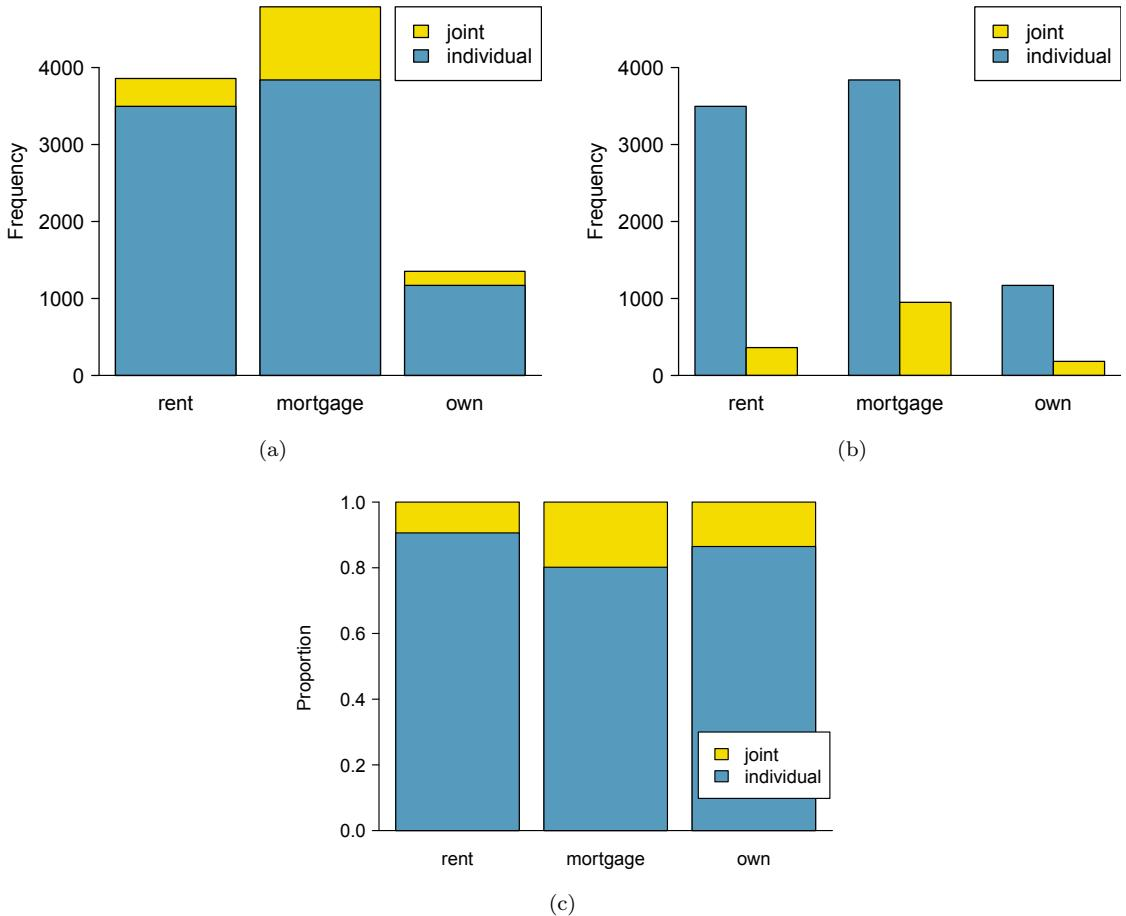
\includegraphics{_page_63_Figure_6.jpeg}

Figura 2.23: \hyperref[page-63-0]{(a)} Diagrama de barras apiladas para
la propiedad de la vivienda, donde los conteos se han desglosado aún más
por tipo de aplicación. \hyperref[page-63-1]{(b)} Diagrama de barras
lado a lado para la propiedad de la vivienda y el tipo de aplicación.
\hyperref[page-63-2]{(c)} Versión estandarizada del diagrama de barras
apiladas.

\section{2.2. CONSIDERANDO DATOS CATEGÓRICOS
65}\label{considerando-datos-categuxf3ricos-65}

\section{\texorpdfstring{\textbf{EJEMPLO
2.27}}{EJEMPLO 2.27}}\label{ejemplo-2.27}

Examine los tres gráficos de barras en la Figura
\hyperref[page-63-3]{2.23.} ¿Cuándo es más útil el gráfico de barras
apiladas, lado a lado o apiladas estandarizadas?

El gráfico de barras apiladas es más útil cuando es razonable asignar
una variable como variable explicativa y la otra variable como
respuesta, ya que estamos agrupando efectivamente por una variable
primero y luego dividiéndola por las otras.

Los gráficos de barras lado a lado son más agnósticos en su
visualización sobre qué variable, si la hay, representa la variable
explicativa y cuál la variable de respuesta. También es fácil discernir
el número de casos en las seis combinaciones de grupos diferentes. Sin
embargo, una desventaja es que tiende a requerir más espacio horizontal;
la estrechez de la Figura \hyperref[page-63-1]{2.23(b)} hace que el
gráfico se sienta un poco apretado. Además, cuando dos grupos son de
tamaños muy diferentes, como vemos en el grupo propio en relación con
cualquiera de los otros dos grupos, es difícil discernir si existe una
asociación entre las variables.

El gráfico de barras apiladas estandarizadas es útil si la variable
primaria en el gráfico de barras apiladas está relativamente
desequilibrada, por ejemplo, la categoría propia tiene solo un tercio de
las observaciones en la categoría de hipoteca, lo que hace que el
gráfico de barras apiladas simple sea menos útil para verificar una
asociación. La principal desventaja de la versión estandarizada es que
perdemos todo sentido de cuántos casos representa cada una de las
barras.

\section{\texorpdfstring{\textbf{2.2.4 Gráficos de
Mosaico}}{2.2.4 Gráficos de Mosaico}}\label{gruxe1ficos-de-mosaico}

Un gráfico de mosaico es una técnica de visualización adecuada para
tablas de contingencia que se asemeja a un gráfico de barras apiladas
estandarizado con el beneficio de que también vemos los tamaños de grupo
relativos de la variable primaria.

Para comenzar a crear nuestro primer gráfico de mosaico, dividiremos un
cuadrado en columnas para cada categoría de la variable de propiedad de
la vivienda, con el resultado que se muestra en la Figura
\hyperref[page-64-0]{2.24(a).} Cada columna representa un nivel de
propiedad de la vivienda, y los anchos de las columnas corresponden a la
proporción de préstamos en cada una de esas categorías. Por ejemplo, hay
menos préstamos donde el prestatario es propietario que donde el
prestatario tiene una hipoteca. En general, los gráficos de mosaico
utilizan áreas de caja para representar el número de casos en cada
categoría.

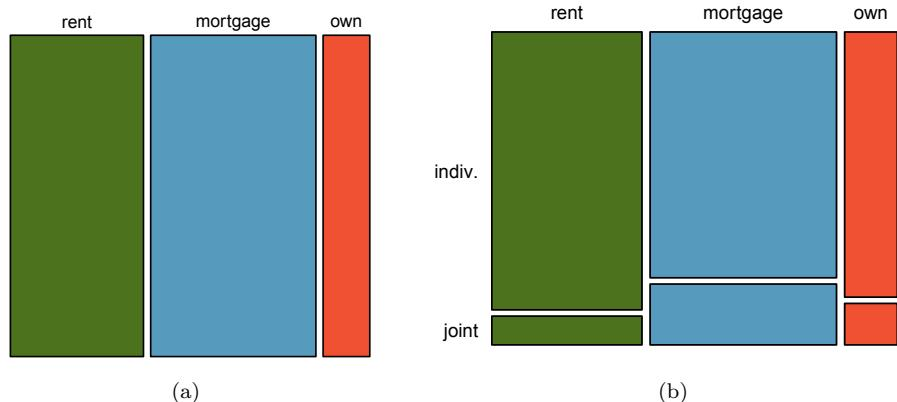
\includegraphics{_page_64_Figure_9.jpeg}

Figura 2.24: \hyperref[page-64-0]{(a)} El gráfico de mosaico de una
variable para la propiedad de la vivienda. \hyperref[page-64-1]{(b)}
Gráfico de mosaico de dos variables para la propiedad de la vivienda y
el tipo de solicitud.

Para crear un gráfico de mosaico completo, el gráfico de mosaico de una
sola variable se divide aún más en piezas en la Figura
\hyperref[page-64-1]{2.24(b)} utilizando la variable de tipo de
solicitud. Cada columna se divide proporcionalmente al número de
préstamos de prestatarios individuales y conjuntos. Por ejemplo, la
segunda columna representa los préstamos en los que el prestatario tiene
una hipoteca, y se dividió en préstamos individuales (superior) y
préstamos conjuntos (inferior). Como otro ejemplo, el segmento inferior
de la tercera columna representa los préstamos en los que el prestatario
es dueño de su casa y solicitó conjuntamente, mientras que el segmento
superior de esta columna representa a los prestatarios que son
propietarios de viviendas y presentaron la solicitud individualmente.
Podemos volver a utilizar este gráfico para ver que las variables de
propiedad de la vivienda y tipo de solicitud están asociadas, ya que
algunas columnas se dividen en diferentes

ubicaciones verticales que otras, que era la misma técnica utilizada
para comprobar una asociación en el gráfico de barras apiladas
estandarizado.

En la Figura \hyperref[page-64-2]{2.24,} elegimos primero dividir por el
estado de propietario de la vivienda del prestatario. Sin embargo,
podríamos haber dividido primero por el tipo de solicitud, como en la
Figura \hyperref[page-65-0]{2.25.} Al igual que con los gráficos de
barras, es común utilizar la variable explicativa para representar la
primera división en un gráfico de mosaico, y luego que la respuesta
divida cada nivel de la variable explicativa, si estas etiquetas son
razonables para adjuntar a las variables en consideración.

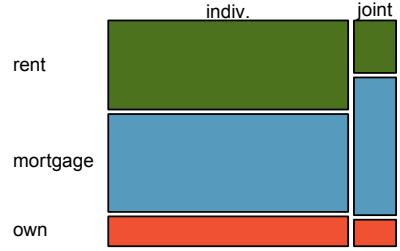
\includegraphics{_page_65_Figure_3.jpeg}

Figura 2.25: Gráfico de mosaico donde los préstamos se agrupan por la
variable de propiedad de la vivienda después de haber sido divididos en
los tipos de solicitud individual y conjunta.

\section{\texorpdfstring{\textbf{2.2.5 El único gráfico circular que
verás en este
libro}}{2.2.5 El único gráfico circular que verás en este libro}}\label{el-uxfanico-gruxe1fico-circular-que-veruxe1s-en-este-libro}

Se muestra un gráfico circular en la Figura \hyperref[page-65-1]{2.26}
junto con un diagrama de barras que representa la misma información. Los
gráficos circulares pueden ser útiles para proporcionar una visión
general de alto nivel que muestre cómo se desglosa un conjunto de casos.
Sin embargo, también es difícil descifrar los detalles en un gráfico
circular. Por ejemplo, se tarda un par de segundos más en reconocer que
hay más préstamos donde el prestatario tiene una hipoteca que alquiler
al mirar el gráfico circular, mientras que este detalle es muy obvio en
el diagrama de barras. Si bien los gráficos circulares pueden ser
útiles, preferimos los diagramas de barras por su facilidad para
comparar grupos.

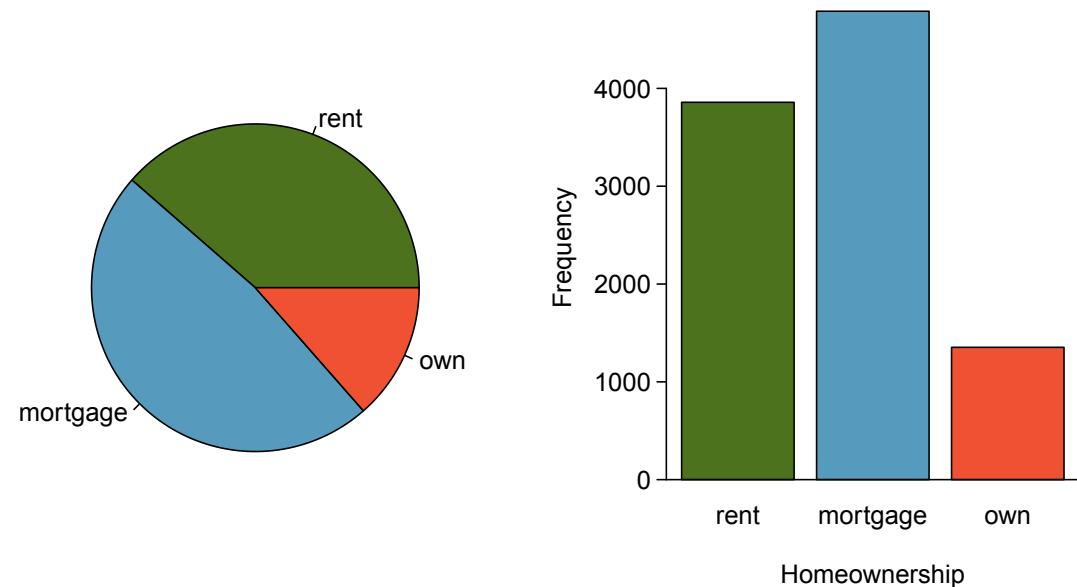
\includegraphics{_page_65_Figure_7.jpeg}

Figura 2.26: Un gráfico circular y un diagrama de barras de la propiedad
de la vivienda.

\section{\texorpdfstring{\textbf{2.2.6 Comparación de datos numéricos
entre
grupos}}{2.2.6 Comparación de datos numéricos entre grupos}}\label{comparaciuxf3n-de-datos-numuxe9ricos-entre-grupos}

Algunas de las investigaciones más interesantes se pueden considerar
examinando los datos numéricos entre grupos. Los métodos requeridos aquí
no son realmente nuevos: todo lo que se requiere es hacer un gráfico
numérico para cada grupo en el mismo gráfico. Aquí se introducen dos
métodos convenientes: diagramas de caja lado a lado e histogramas
huecos.

Volveremos a ver el conjunto de datos del condado y compararemos el
ingreso familiar medio para los condados que ganaron población de 2010 a
2017 frente a los condados que no tuvieron ganancias. Si bien nos
gustaría hacer una conexión causal aquí, recuerde que estos son datos de
observación y, por lo tanto, tal interpretación sería, en el mejor de
los casos, a medias.

Hubo 1,454 condados donde la población aumentó de 2010 a 2017, y hubo
1,672 condados sin ganancia (todos menos uno fueron una pérdida). Una
muestra aleatoria de 100 condados del primer grupo y 50 del segundo
grupo se muestra en la Figura \hyperref[page-66-0]{2.27} para dar una
mejor idea de algunos de los datos brutos de ingresos medios.

\begin{longtable}[]{@{}
  >{\raggedright\arraybackslash}p{(\columnwidth - 16\tabcolsep) * \real{0.1111}}
  >{\raggedright\arraybackslash}p{(\columnwidth - 16\tabcolsep) * \real{0.1111}}
  >{\raggedright\arraybackslash}p{(\columnwidth - 16\tabcolsep) * \real{0.1111}}
  >{\raggedright\arraybackslash}p{(\columnwidth - 16\tabcolsep) * \real{0.1111}}
  >{\raggedright\arraybackslash}p{(\columnwidth - 16\tabcolsep) * \real{0.1111}}
  >{\raggedright\arraybackslash}p{(\columnwidth - 16\tabcolsep) * \real{0.1111}}
  >{\raggedright\arraybackslash}p{(\columnwidth - 16\tabcolsep) * \real{0.1111}}
  >{\raggedright\arraybackslash}p{(\columnwidth - 16\tabcolsep) * \real{0.1111}}
  >{\raggedright\arraybackslash}p{(\columnwidth - 16\tabcolsep) * \real{0.1111}}@{}}
\toprule\noalign{}
\begin{minipage}[b]{\linewidth}\raggedright
Ganancia de población
\end{minipage} & \begin{minipage}[b]{\linewidth}\raggedright
\end{minipage} & \begin{minipage}[b]{\linewidth}\raggedright
\end{minipage} & \begin{minipage}[b]{\linewidth}\raggedright
\end{minipage} & \begin{minipage}[b]{\linewidth}\raggedright
\end{minipage} & \begin{minipage}[b]{\linewidth}\raggedright
Sin ganancia de población
\end{minipage} & \begin{minipage}[b]{\linewidth}\raggedright
\end{minipage} & \begin{minipage}[b]{\linewidth}\raggedright
\end{minipage} & \begin{minipage}[b]{\linewidth}\raggedright
\end{minipage} \\
\midrule\noalign{}
\endhead
\bottomrule\noalign{}
\endlastfoot
38.2 & 43.6 & 42.2 & 61.5 & 51.1 & 45.7 & 48.3 & 60.3 & 50.7 \\
44.6 & 51.8 & 40.7 & 48.1 & 56.4 & 41.9 & 39.3 & 40.4 & 40.3 \\
40.6 & 63.3 & 52.1 & 60.3 & 49.8 & 51.7 & 57 & 47.2 & 45.9 \\
51.1 & 34.1 & 45.5 & 52.8 & 49.1 & 51 & 42.3 & 41.5 & 46.1 \\
80.8 & 46.3 & 82.2 & 43.6 & 39.7 & 49.4 & 44.9 & 51.7 & 46.4 \\
75.2 & 40.6 & 46.3 & 62.4 & 44.1 & 51.3 & 29.1 & 51.8 & 50.5 \\
51.9 & 34.7 & 54 & 42.9 & 52.2 & 45.1 & 27 & 30.9 & 34.9 \\
61 & 51.4 & 56.5 & 62 & 46 & 46.4 & 40.7 & 51.8 & 61.1 \\
53.8 & 57.6 & 69.2 & 48.4 & 40.5 & 48.6 & 43.4 & 34.7 & 45.7 \\
53.1 & 54.6 & 55 & 46.4 & 39.9 & 56.7 & 33.1 & 21 & 37 \\
63 & 49.1 & 57.2 & 44.1 & 50 & 38.9 & 52 & 31.9 & 45.7 \\
46.6 & 46.5 & 38.9 & 50.9 & 56 & 34.6 & 56.3 & 38.7 & 45.7 \\
74.2 & 63 & 49.6 & 53.7 & 77.5 & 60 & 56.2 & 43 & 21.7 \\
63.2 & 47.6 & 55.9 & 39.1 & 57.8 & 42.6 & 44.5 & 34.5 & 48.9 \\
50.4 & 49 & 45.6 & 39 & 38.8 & 37.1 & 50.9 & 42.1 & 43.2 \\
57.2 & 44.7 & 71.7 & 35.3 & 100.2 & & 35.4 & 41.3 & 33.6 \\
42.6 & 55.5 & 38.6 & 52.7 & 63 & & 43.4 & 56.5 & \\
\end{longtable}

Ingreso medio para 150 condados, en \$1000

Figura 2.27: En esta tabla, se muestra el ingreso familiar medio (en
\$1000) de una muestra aleatoria de 100 condados que tuvieron ganancias
de población a la izquierda. Los ingresos medios de una muestra
aleatoria de 50 condados que no tuvieron ganancias de población se
muestran a la derecha.

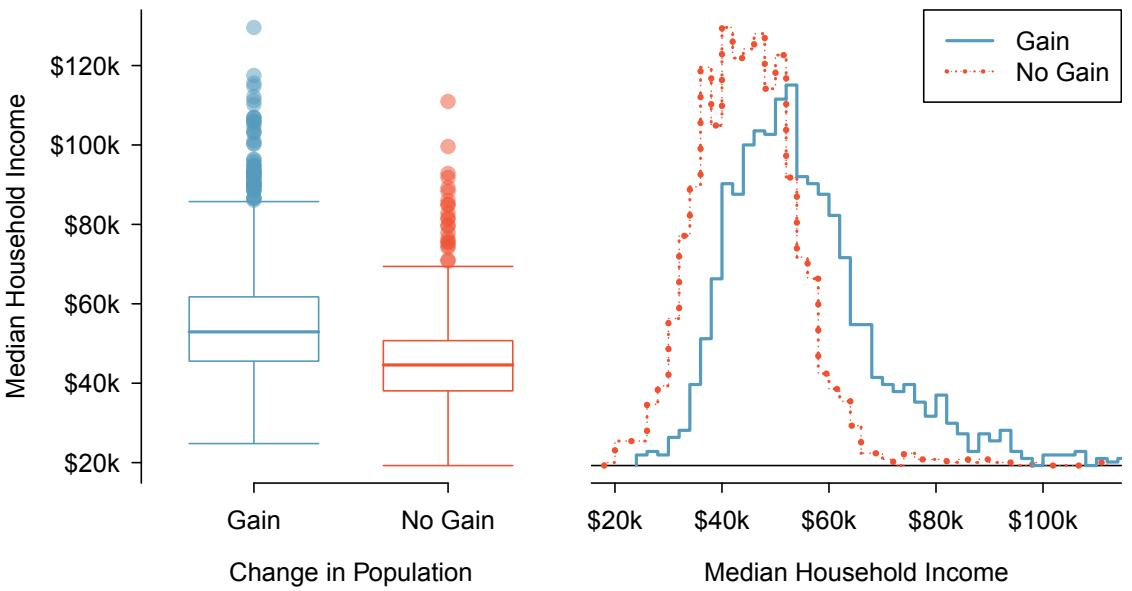
\includegraphics{_page_67_Figure_1.jpeg}

Figura 2.28: Diagrama de caja lado a lado (panel izquierdo) e
histogramas huecos (panel derecho) para el ingreso familiar medio, donde
los condados se dividen por si hubo una ganancia de población o si no
hubo ganancia.

El diagrama de caja lado a lado es una herramienta tradicional para
comparar entre grupos. Se muestra un ejemplo en el panel izquierdo de la
Figura \hyperref[page-67-0]{2.28,} donde hay dos diagramas de caja, uno
para cada grupo, colocados en una ventana de trazado y dibujados en la
misma escala.

Otro método de trazado útil utiliza histogramas huecos para comparar
datos numéricos entre grupos. Estos son solo los contornos de los
histogramas de cada grupo colocados en el mismo gráfico, como se muestra
en el panel derecho de la Figura \hyperref[page-67-0]{2.28.}

\subsection{\texorpdfstring{\textbf{PRÁCTICA GUIADA
2.28}}{PRÁCTICA GUIADA 2.28}}\label{pruxe1ctica-guiada-2.28}

Utilice los gráficos de la Figura \hyperref[page-67-0]{2.28} para
comparar los ingresos de los condados entre los dos grupos. ¿Qué nota
sobre el centro aproximado de cada grupo? ¿Qué nota sobre la
variabilidad entre grupos? ¿Es la forma relativamente consistente entre
los grupos? ¿Cuántos modos prominentes hay para cada
grupo?\hyperref[page-67-1]{20}

\paragraph{\texorpdfstring{\textbf{PRÁCTICA GUIADA
2.29}}{PRÁCTICA GUIADA 2.29}}\label{pruxe1ctica-guiada-2.29}

¿Qué componentes de cada gráfico en la Figura \hyperref[page-67-0]{2.28}
le resultan más útiles?\hyperref[page-67-2]{21}

20Las respuestas pueden variar un poco. Los condados con ganancias de
población tienden a tener ingresos más altos (mediana de alrededor de
\$45,000) en comparación con los condados sin ganancias (mediana de
alrededor de \$40,000). La variabilidad también es ligeramente mayor
para el grupo de ganancia de población. Esto es evidente en el IQR, que
es aproximadamente un 50\% mayor en el grupo de ganancia. Ambas
distribuciones muestran una ligera a moderada asimetría hacia la derecha
y son unimodales. Los diagramas de caja indican que hay muchas
observaciones muy por encima de la mediana en cada grupo, aunque
deberíamos anticipar que muchas observaciones caerán más allá de los
bigotes al examinar cualquier conjunto de datos que contenga más de un
par de cientos de puntos de datos.

21Las respuestas variarán. Los diagramas de caja lado a lado son
especialmente útiles para comparar centros y extensiones, mientras que
los histogramas huecos son más útiles para ver la forma de la
distribución, la asimetría y las posibles anomalías.

\section{\texorpdfstring{\textbf{Ejercicios}}{Ejercicios}}\label{ejercicios-3}

\hyperref[page-385-12]{\textbf{2.21}} \textbf{Uso de antibióticos en
niños.} El gráfico de barras y el gráfico circular a continuación
muestran la distribución de las afecciones médicas preexistentes de los
niños involucrados en un estudio sobre la duración óptima del uso de
antibióticos en el tratamiento de la traqueítis, que es una infección
del tracto respiratorio superior.

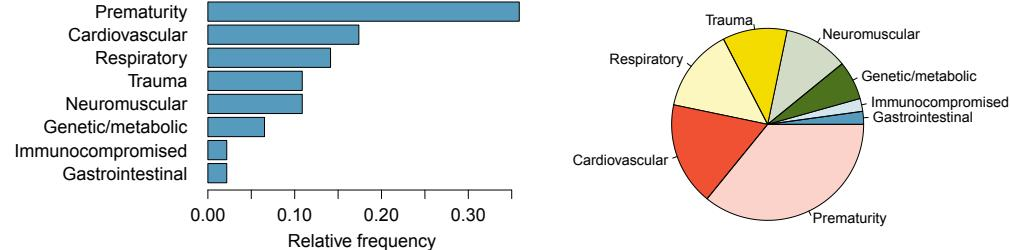
\includegraphics{_page_68_Figure_3.jpeg}

\begin{itemize}
\tightlist
\item
  \begin{enumerate}
  \def\labelenumi{(\alph{enumi})}
  \tightlist
  \item
    ¿Qué características son evidentes en el gráfico de barras pero no
    en el gráfico circular?
  \end{enumerate}
\item
  \begin{enumerate}
  \def\labelenumi{(\alph{enumi})}
  \setcounter{enumi}{1}
  \tightlist
  \item
    ¿Qué características son evidentes en el gráfico circular pero no en
    el gráfico de barras?
  \end{enumerate}
\item
  \begin{enumerate}
  \def\labelenumi{(\alph{enumi})}
  \setcounter{enumi}{2}
  \tightlist
  \item
    ¿Qué gráfico preferiría utilizar para mostrar estos datos
    categóricos?
  \end{enumerate}
\end{itemize}

\hyperref[page-385-13]{\textbf{2.22}} \textbf{Opiniones sobre la
inmigración.} Se preguntó a 910 votantes registrados seleccionados al
azar de Tampa, FL, si pensaban que los trabajadores que habían ingresado
ilegalmente a los EE. UU. deberían (i) poder conservar sus trabajos y
solicitar la ciudadanía estadounidense, (ii) poder conservar sus
trabajos como trabajadores huéspedes temporales pero no poder solicitar
la ciudadanía estadounidense, o (iii) perder sus trabajos y tener que
salir del país. Los resultados de la encuesta por ideología política se
muestran a continuación.\hyperref[page-68-0]{22}

\begin{longtable}[]{@{}llllll@{}}
\toprule\noalign{}
& & Ideología política & & & \\
\midrule\noalign{}
\endhead
\bottomrule\noalign{}
\endlastfoot
& & Conservador & Moderado & Liberal & Total \\
Respuesta & (i) Solicitar la ciudadanía & 57 & 120 & 101 & 278 \\
& (ii) Trabajador huésped & 121 & 113 & 28 & 262 \\
& (iii) Salir del país & 179 & 126 & 45 & 350 \\
& (iv) No estoy seguro & 15 & 4 & 1 & 20 \\
& Total & 372 & 363 & 175 & 910 \\
\end{longtable}

\begin{itemize}
\tightlist
\item
  \begin{enumerate}
  \def\labelenumi{(\alph{enumi})}
  \tightlist
  \item
    ¿Qué porcentaje de estos votantes de Tampa, FL, se identifican como
    conservadores?
  \end{enumerate}
\item
  \begin{enumerate}
  \def\labelenumi{(\alph{enumi})}
  \setcounter{enumi}{1}
  \tightlist
  \item
    ¿Qué porcentaje de estos votantes de Tampa, FL, está a favor de la
    opción de ciudadanía?
  \end{enumerate}
\item
  \begin{enumerate}
  \def\labelenumi{(\alph{enumi})}
  \setcounter{enumi}{2}
  \tightlist
  \item
    ¿Qué porcentaje de estos votantes de Tampa, FL, se identifican como
    conservadores y están a favor de la opción de ciudadanía?
  \end{enumerate}
\item
  \begin{enumerate}
  \def\labelenumi{(\alph{enumi})}
  \setcounter{enumi}{3}
  \tightlist
  \item
    ¿Qué porcentaje de estos votantes de Tampa, FL, que se identifican
    como conservadores también están a favor de la opción de ciudadanía?
    ¿Qué porcentaje de moderados comparte esta opinión? ¿Qué porcentaje
    de liberales comparte esta opinión?
  \end{enumerate}
\item
  \begin{enumerate}
  \def\labelenumi{(\alph{enumi})}
  \setcounter{enumi}{4}
  \tightlist
  \item
    ¿Parecen ser independientes la ideología política y las opiniones
    sobre la inmigración? Explique su razonamiento.
  \end{enumerate}
\end{itemize}

22SurveyUSA,
\href{http://www.openintro.org/redirect.php?go=textbook-SurveyUSA_18927&referrer=os4_pdf}{Encuesta
de noticias \#18927,} datos recopilados del 27 al 29 de enero de 2012.

\hyperref[page-385-14]{\textbf{2.23}} \textbf{Opiniones sobre la Ley
DREAM.} Se preguntó a una muestra aleatoria de votantes registrados de
Tampa, FL, si apoyaban la Ley DREAM, una ley propuesta que
proporcionaría un camino hacia la ciudadanía para las personas llevadas
ilegalmente a los EE. UU. cuando eran niños. La encuesta también
recopiló información sobre la ideología política de los encuestados.
Según el diagrama de mosaico que se muestra a continuación, ¿parecen ser
independientes las opiniones sobre la Ley DREAM y la ideología política?
Explique su razonamiento.\hyperref[page-69-0]{23}

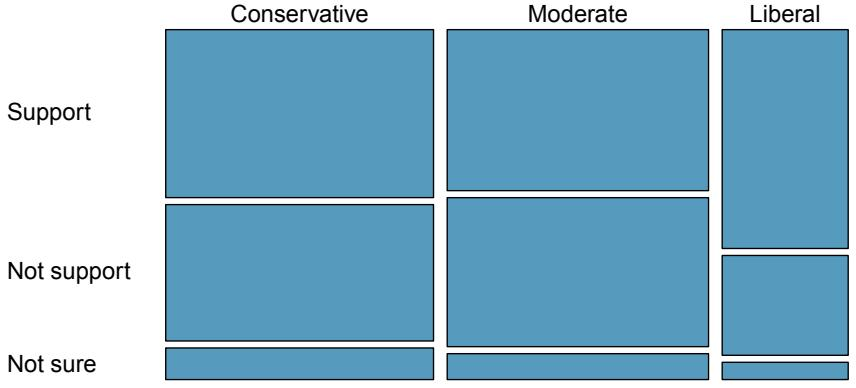
\includegraphics{_page_69_Figure_2.jpeg}

\hyperref[page-385-15]{\textbf{2.24}} \textbf{Aumento de impuestos.} Se
preguntó a una muestra aleatoria de votantes registrados a nivel
nacional si pensaban que era mejor aumentar los impuestos a los ricos o
aumentar los impuestos a los pobres. La encuesta también recopiló
información sobre la afiliación al partido político de los encuestados.
Según el diagrama de mosaico que se muestra a continuación, ¿parecen ser
independientes las opiniones sobre el aumento de impuestos y la
afiliación política? Explique su razonamiento.\hyperref[page-69-1]{24}

\includegraphics{_page_69_Figure_4.jpeg}

23SurveyUSA,
\href{http://www.openintro.org/redirect.php?go=textbook-SurveyUSA_18927&referrer=os4_pdf}{Encuesta
de noticias \#18927,} datos recopilados del 27 al 29 de enero de 2012.

24Public Policy Polling,
\href{http://www.openintro.org/redirect.php?go=textbook-PPP_30215&referrer=os4_pdf}{Estadounidenses
sobre títulos universitarios, literatura clásica, las estaciones y más,}
datos recopilados del 20 al 22 de febrero de 2015.

\section{\texorpdfstring{\textbf{2.3 Estudio de caso: vacuna contra la
malaria}}{2.3 Estudio de caso: vacuna contra la malaria}}\label{estudio-de-caso-vacuna-contra-la-malaria}

\paragraph{\texorpdfstring{\textbf{EJEMPLO
2.30}}{EJEMPLO 2.30}}\label{ejemplo-2.30}

Supongamos que su profesor divide a los estudiantes de la clase en dos
grupos: los estudiantes de la izquierda y los estudiantes de la derecha.
Si ˆpL y ˆpR representan la proporción de estudiantes que poseen un
producto Apple a la izquierda y a la derecha, respectivamente, ¿le
sorprendería que ˆpL no fuera exactamente igual a ˆpR ?

Si bien las proporciones probablemente serían cercanas entre sí, sería
inusual que fueran exactamente iguales. Probablemente observaríamos una
pequeña diferencia debido al azar.

\paragraph{\texorpdfstring{\textbf{PRÁCTICA GUIADA
2.31}}{PRÁCTICA GUIADA 2.31}}\label{pruxe1ctica-guiada-2.31}

Si no creemos que el lado de la sala en el que se sienta una persona en
clase esté relacionado con si la persona posee o no un producto Apple,
¿qué suposición estamos haciendo sobre la relación entre estas dos
variables?\hyperref[page-70-1]{25}

\section{\texorpdfstring{\textbf{2.3.1 Variabilidad dentro de los
datos}}{2.3.1 Variabilidad dentro de los datos}}\label{variabilidad-dentro-de-los-datos}

Consideramos un estudio sobre una nueva vacuna contra la malaria llamada
PfSPZ. En este estudio, pacientes voluntarios fueron aleatorizados en
uno de dos grupos experimentales: 14 pacientes recibieron una vacuna
experimental y 6 pacientes recibieron una vacuna placebo. Diecinueve
semanas después, los 20 pacientes fueron expuestos a una cepa de
parásito de la malaria sensible a los fármacos; la motivación de usar
una cepa de parásito sensible a los fármacos aquí es por consideraciones
éticas, lo que permite que cualquier infección sea tratada eficazmente.
Los resultados se resumen en la Figura \hyperref[page-70-2]{2.29,} donde
9 de los 14 pacientes tratados permanecieron libres de signos de
infección, mientras que los 6 pacientes del grupo de control mostraron
algunos signos de infección basales.

\begin{longtable}[]{@{}
  >{\raggedright\arraybackslash}p{(\columnwidth - 14\tabcolsep) * \real{0.1711}}
  >{\raggedright\arraybackslash}p{(\columnwidth - 14\tabcolsep) * \real{0.3553}}
  >{\raggedright\arraybackslash}p{(\columnwidth - 14\tabcolsep) * \real{0.1447}}
  >{\raggedright\arraybackslash}p{(\columnwidth - 14\tabcolsep) * \real{0.0658}}
  >{\raggedright\arraybackslash}p{(\columnwidth - 14\tabcolsep) * \real{0.0658}}
  >{\raggedright\arraybackslash}p{(\columnwidth - 14\tabcolsep) * \real{0.0658}}
  >{\raggedright\arraybackslash}p{(\columnwidth - 14\tabcolsep) * \real{0.0658}}
  >{\raggedright\arraybackslash}p{(\columnwidth - 14\tabcolsep) * \real{0.0658}}@{}}
\toprule\noalign{}
\begin{minipage}[b]{\linewidth}\raggedright
\end{minipage} & \begin{minipage}[b]{\linewidth}\raggedright
\end{minipage} & \begin{minipage}[b]{\linewidth}\raggedright
resultado
\end{minipage} & \begin{minipage}[b]{\linewidth}\raggedright
\end{minipage} & \begin{minipage}[b]{\linewidth}\raggedright
\end{minipage} & \begin{minipage}[b]{\linewidth}\raggedright
\end{minipage} & \begin{minipage}[b]{\linewidth}\raggedright
\end{minipage} & \begin{minipage}[b]{\linewidth}\raggedright
\end{minipage} \\
\midrule\noalign{}
\endhead
\bottomrule\noalign{}
\endlastfoot
& infecciónno infección & & & & & & \\
tratamiento & vacuna & 5 & 9 & 14 & & & \\
& placebo & 6 & 0 & 6 & & & \\
& Total & 11 & 9 & 20 & & & \\
\end{longtable}

Figura 2.29: Resultados resumidos para el experimento de la vacuna
contra la malaria.

\paragraph{\texorpdfstring{\textbf{PRÁCTICA GUIADA
2.32}}{PRÁCTICA GUIADA 2.32}}\label{pruxe1ctica-guiada-2.32}

¿Es este un estudio observacional o un experimento? ¿Qué implicaciones
tiene el tipo de estudio sobre lo que se puede inferir de los
resultados?\hyperref[page-70-3]{26}

En este estudio, una proporción menor de pacientes que recibieron la
vacuna mostraron signos de infección (35.7\% versus 100\%). Sin embargo,
la muestra es muy pequeña y no está claro si la diferencia proporciona
evidencia convincente de que la vacuna es eficaz.

25Estaríamos asumiendo que estas dos variables son independientes.

26El estudio es un experimento, ya que los pacientes fueron asignados
aleatoriamente a un grupo experimental. Dado que este es un experimento,
los resultados se pueden utilizar para evaluar una relación causal entre
la vacuna contra la malaria y si los pacientes mostraron signos de
infección.

\section{\texorpdfstring{\textbf{EJEMPLO
2.33}}{EJEMPLO 2.33}}\label{ejemplo-2.33}

A veces se solicita a los científicos de datos que evalúen la solidez de
la evidencia. Al observar las tasas de infección de los pacientes en los
dos grupos en este estudio, ¿qué se nos viene a la mente mientras
intentamos determinar si los datos muestran evidencia convincente de una
diferencia real?

Las tasas de infección observadas (35.7\% para el grupo de tratamiento
versus 100\% para el grupo de control) sugieren que la vacuna puede ser
eficaz. Sin embargo, no podemos estar seguros de si la diferencia
observada representa la eficacia de la vacuna o si se debe simplemente
al azar. Generalmente, hay un poco de fluctuación en los datos de la
muestra, y no esperaríamos que las proporciones de la muestra sean
exactamente iguales, incluso si la verdad fuera que las tasas de
infección fueran independientes de la vacunación. Además, con muestras
tan pequeñas, ¡quizás es común observar diferencias tan grandes cuando
dividimos aleatoriamente un grupo debido solo al azar!

El ejemplo \hyperref[page-71-0]{2.33} es un recordatorio de que los
resultados observados en la muestra de datos pueden no reflejar
perfectamente las verdaderas relaciones entre las variables, ya que hay
ruido aleatorio. Si bien la diferencia observada en las tasas de
infección es grande, el tamaño de la muestra para el estudio es pequeño,
lo que hace que no esté claro si esta diferencia observada representa la
eficacia de la vacuna o si se debe simplemente al azar. Etiquetamos
estas dos afirmaciones contrapuestas, H0 y HA, que se pronuncian como
``H-cero'' y ``H-A'':

\begin{itemize}
\tightlist
\item
  H0: Modelo de independencia. Las variables tratamiento y resultado son
  independientes. No tienen relación, y la diferencia observada entre la
  proporción de pacientes que desarrollaron una infección en los dos
  grupos, 64.3\%, se debió al azar.
\item
  HA: Modelo alternativo. Las variables no son independientes. La
  diferencia en las tasas de infección del 64.3\% no se debió al azar, y
  la vacuna afectó la tasa de infección.
\end{itemize}

¿Qué significaría si el modelo de independencia, que dice que la vacuna
no tuvo influencia en la tasa de infección, fuera cierto? Significaría
que 11 pacientes iban a desarrollar una infección sin importar en qué
grupo fueran aleatorizados, y 9 pacientes no desarrollarían una
infección sin importar en qué grupo fueran aleatorizados. Es decir, si
la vacuna no afectara la tasa de infección, la diferencia en las tasas
de infección se debería solo al azar en cómo se aleatorizaron los
pacientes.

Ahora considere el modelo alternativo: las tasas de infección fueron
influenciadas por si un paciente recibió la vacuna o no. Si esto fuera
cierto, y especialmente si esta influencia fuera sustancial,
esperaríamos ver alguna diferencia en las tasas de infección de los
pacientes en los grupos.

Elegimos entre estas dos afirmaciones contrapuestas evaluando si los
datos están tan en conflicto con H0 que el modelo de independencia no
puede considerarse razonable. Si este es el caso, y los datos apoyan HA,
entonces rechazaremos la noción de independencia y concluiremos que la
vacuna fue eficaz.

\section{\texorpdfstring{\textbf{2.3.2 Simulando el
estudio}}{2.3.2 Simulando el estudio}}\label{simulando-el-estudio}

Vamos a implementar simulaciones, donde fingiremos que sabemos que la
vacuna contra la malaria que se está probando no funciona. En última
instancia, queremos entender si la gran diferencia que observamos es
común en estas simulaciones. Si es común, entonces tal vez la diferencia
que observamos se debió puramente al azar. Si es muy poco común,
entonces la posibilidad de que la vacuna haya sido útil parece más
plausible.

La Figura \hyperref[page-70-2]{2.29} muestra que 11 pacientes
desarrollaron infecciones y 9 no. Para nuestra simulación, supondremos
que las infecciones fueron independientes de la vacuna y que pudimos
retroceder a cuando los investigadores aleatorizaron a los pacientes en
el estudio. Si hubiéramos aleatorizado a los pacientes de manera
diferente, podríamos obtener un resultado diferente en este mundo
hipotético donde la vacuna no influye en la infección. Completemos otra
aleatorización usando una simulación.

\section{2.3. CASO DE ESTUDIO: VACUNA CONTRA LA MALARIA
73}\label{caso-de-estudio-vacuna-contra-la-malaria-73}

En esta simulación, tomamos 20 fichas para representar a los 20
pacientes, donde escribimos ``infección'' en 11 fichas y ``sin
infección'' en 9 fichas. En este mundo hipotético, creemos que cada
paciente que contrajo una infección la iba a contraer independientemente
del grupo en el que estuviera, así que veamos qué sucede si asignamos
aleatoriamente a los pacientes a los grupos de tratamiento y control
nuevamente. Barajamos a fondo las fichas y repartimos 14 en una pila de
vacunas y 6 en una pila de placebo. Finalmente, tabulamos los
resultados, que se muestran en la Figura \hyperref[page-72-0]{2.30.}

\begin{longtable}[]{@{}lllll@{}}
\toprule\noalign{}
& & resultado & & \\
\midrule\noalign{}
\endhead
\bottomrule\noalign{}
\endlastfoot
& & infección & no infección & Total \\
tratamiento & vacuna & 7 & 7 & 14 \\
(simulado) & placebo & 4 & 2 & 6 \\
& Total & 11 & 9 & 20 \\
\end{longtable}

Figura 2.30: Resultados de la simulación, donde cualquier diferencia en
las tasas de infección se debe puramente al azar.

\section{\texorpdfstring{\textbf{PRÁCTICA GUIADA
2.34}}{PRÁCTICA GUIADA 2.34}}\label{pruxe1ctica-guiada-2.34}

¿Cuál es la diferencia en las tasas de infección entre los dos grupos
simulados en la Figura \hyperref[page-72-0]{2.30?} ¿Cómo se compara esto
con la diferencia observada del 64.3\% en los datos
reales?\hyperref[page-72-1]{27}

\section{\texorpdfstring{\textbf{2.3.3 Comprobación de la
independencia}}{2.3.3 Comprobación de la independencia}}\label{comprobaciuxf3n-de-la-independencia}

En la Práctica Guiada \hyperref[page-72-2]{2.34,} calculamos una posible
diferencia bajo el modelo de independencia, que representa una
diferencia debida al azar. Si bien en esta primera simulación,
repartimos físicamente tarjetas para representar a los pacientes, es más
eficiente realizar esta simulación usando una computadora. Al repetir la
simulación en una computadora, obtenemos otra diferencia debida al azar:

\[\frac{2}{6} - \frac{9}{14} = -0.310\]

Y otra:

\[\frac{3}{6} - \frac{8}{14} = -0.071\]

Y así sucesivamente hasta que repitamos la simulación suficientes veces
para tener una buena idea de lo que representa la distribución de las
diferencias debidas únicamente al azar. La Figura
\hyperref[page-73-0]{2.31} muestra un gráfico apilado de las diferencias
encontradas a partir de 100 simulaciones, donde cada punto representa
una diferencia simulada entre las tasas de infección (tasa de control
menos tasa de tratamiento).

Observe que la distribución de estas diferencias simuladas está centrada
alrededor de 0. Simulamos estas diferencias asumiendo que el modelo de
independencia era verdadero, y bajo esta condición, esperamos que la
diferencia esté cerca de cero con alguna fluctuación aleatoria, donde
cerca es bastante generoso en este caso ya que los tamaños de muestra
son tan pequeños en este estudio.

\section{\texorpdfstring{\textbf{EJEMPLO
2.35}}{EJEMPLO 2.35}}\label{ejemplo-2.35}

¿Con qué frecuencia observaría una diferencia de al menos 64.3\% (0.643)
según la Figura \hyperref[page-73-0]{2.31?} ¿A menudo, a veces,
raramente o nunca?

Parece que una diferencia de al menos 64.3\% debida solo al azar
ocurriría solo alrededor del 2\% de las veces según la Figura
\hyperref[page-73-0]{2.31.} Una probabilidad tan baja indica un evento
raro.

274/6 − 7/14 = 0.167 o aproximadamente 16.7\% a favor de la vacuna. Esta
diferencia debida al azar es mucho menor que la diferencia observada en
los grupos reales.

\includegraphics{_page_73_Figure_1.jpeg}

Diferencia en las tasas de infección

Figura 2.31: Un diagrama de puntos apilados de las diferencias de 100
simulaciones producidas bajo el modelo de independencia, H0, donde en
estas simulaciones las infecciones no se ven afectadas por la vacuna.
Dos de las 100 simulaciones tuvieron una diferencia de al menos 64.3\%,
la diferencia observada en el estudio.

La diferencia del 64.3\% como un evento raro sugiere dos posibles
interpretaciones de los resultados del estudio:

\begin{itemize}
\tightlist
\item
  H0 Modelo de Independencia. La vacuna no tiene ningún efecto sobre la
  tasa de infección, y simplemente observamos una diferencia que solo
  ocurriría en una ocasión rara.
\item
  HA Modelo Alternativo. La vacuna tiene un efecto sobre la tasa de
  infección, y la diferencia que observamos se debió en realidad a que
  la vacuna es eficaz para combatir la malaria, lo que explica la gran
  diferencia de 64.3\%.
\end{itemize}

Basándonos en las simulaciones, tenemos dos opciones. (1) Concluimos que
los resultados del estudio no proporcionan evidencia sólida en contra
del modelo de independencia. Es decir, no tenemos evidencia
suficientemente sólida para concluir que la vacuna tuvo un efecto en
este entorno clínico. (2) Concluimos que la evidencia es suficientemente
sólida para rechazar H0 y afirmar que la vacuna fue útil. Cuando
realizamos estudios formales, generalmente rechazamos la noción de que
simplemente observamos un evento raro.\hyperref[page-73-1]{28} Entonces,
en este caso, rechazamos el modelo de independencia en favor del
alternativo. Es decir, estamos concluyendo que los datos proporcionan
evidencia sólida de que la vacuna proporciona cierta protección contra
la malaria en este entorno clínico.

Un campo de la estadística, la inferencia estadística, se basa en
evaluar si tales diferencias se deben al azar. En la inferencia
estadística, los científicos de datos evalúan qué modelo es más
razonable dados los datos. Los errores ocurren, al igual que los eventos
raros, y podríamos elegir el modelo equivocado. Si bien no siempre
elegimos correctamente, la inferencia estadística nos brinda
herramientas para controlar y evaluar con qué frecuencia ocurren estos
errores. En el Capítulo \hyperref[page-167-0]{5,} damos una introducción
formal al problema de la selección de modelos. Pasamos los próximos dos
capítulos construyendo una base de probabilidad y teoría necesaria para
que esa discusión sea rigurosa.

28Este razonamiento no se extiende generalmente a las observaciones
anecdóticas. Cada uno de nosotros observa eventos increíblemente raros
todos los días, eventos que no podríamos esperar predecir. Sin embargo,
en el entorno no riguroso de la evidencia anecdótica, casi cualquier
cosa puede parecer un evento raro, por lo que la idea de buscar eventos
raros en las actividades cotidianas es traicionera. Por ejemplo,
podríamos mirar la lotería: ¡solo había 1 entre 292 millones de
posibilidades de que los números de Powerball para el premio mayor más
grande de la historia (13 de enero de 2016) fueran (04, 08, 19, 27, 34)
con un Powerball de (10), pero sin embargo esos números salieron! Sin
embargo, no importa qué números hubieran salido, habrían tenido las
mismas probabilidades increíblemente raras. Es decir, cualquier conjunto
de números que podríamos haber observado sería en última instancia
increíblemente raro. Este tipo de situación es típico de nuestra vida
diaria: cada evento posible en sí mismo parece increíblemente raro, pero
si consideramos cada alternativa, esos resultados también son
increíblemente raros. Debemos tener cuidado de no malinterpretar tal
evidencia anecdótica.

\section{\texorpdfstring{\textbf{Ejercicios}}{Ejercicios}}\label{ejercicios-4}

\hyperref[page-386-0]{\textbf{2.25}} \textbf{Efectos secundarios de
Avandia.} La rosiglitazona es el ingrediente activo de Avandia, un
medicamento controvertido para la diabetes tipo 2, y se ha relacionado
con un mayor riesgo de problemas cardiovasculares graves como accidentes
cerebrovasculares, insuficiencia cardíaca y muerte. Un tratamiento
alternativo común es la pioglitazona, el ingrediente activo de un
medicamento para la diabetes llamado Actos. En un estudio observacional
retrospectivo a nivel nacional de 227,571 beneficiarios de Medicare de
65 años o más, se descubrió que 2,593 de los 67,593 pacientes que usaban
rosiglitazona y 5,386 de los 159,978 que usaban pioglitazona tenían
problemas cardiovasculares graves. Estos datos se resumen en la tabla de
contingencia a continuación.\hyperref[page-74-0]{29}

\begin{longtable}[]{@{}
  >{\raggedright\arraybackslash}p{(\columnwidth - 8\tabcolsep) * \real{0.1757}}
  >{\raggedright\arraybackslash}p{(\columnwidth - 8\tabcolsep) * \real{0.2027}}
  >{\raggedright\arraybackslash}p{(\columnwidth - 8\tabcolsep) * \real{0.3784}}
  >{\raggedright\arraybackslash}p{(\columnwidth - 8\tabcolsep) * \real{0.1216}}
  >{\raggedright\arraybackslash}p{(\columnwidth - 8\tabcolsep) * \real{0.1216}}@{}}
\toprule\noalign{}
\begin{minipage}[b]{\linewidth}\raggedright
\end{minipage} & \begin{minipage}[b]{\linewidth}\raggedright
\end{minipage} & \begin{minipage}[b]{\linewidth}\raggedright
Problemas cardiovasculares
\end{minipage} & \begin{minipage}[b]{\linewidth}\raggedright
\end{minipage} & \begin{minipage}[b]{\linewidth}\raggedright
\end{minipage} \\
\midrule\noalign{}
\endhead
\bottomrule\noalign{}
\endlastfoot
& & Sí & No & Total \\
Tratamiento & Rosiglitazona & 2,593 & 65,000 & 67,593 \\
& Pioglitazona & 5,386 & 154,592 & 159,978 \\
& Total & 7,979 & 219,592 & 227,571 \\
\end{longtable}

\begin{itemize}
\item
  \begin{enumerate}
  \def\labelenumi{(\alph{enumi})}
  \tightlist
  \item
    Determine si cada una de las siguientes afirmaciones es verdadera o
    falsa. Si es falsa, explique por qué. Tenga cuidado: el razonamiento
    puede ser incorrecto incluso si la conclusión de la afirmación es
    correcta. En tales casos, la afirmación debe considerarse falsa.
  \end{enumerate}

  \begin{itemize}
  \tightlist
  \item
    \begin{enumerate}
    \def\labelenumi{\roman{enumi}.}
    \tightlist
    \item
      Dado que más pacientes con pioglitazona tuvieron problemas
      cardiovasculares (5,386 frente a 2,593), podemos concluir que la
      tasa de problemas cardiovasculares para aquellos en un tratamiento
      con pioglitazona es mayor.
    \end{enumerate}
  \item
    \begin{enumerate}
    \def\labelenumi{\roman{enumi}.}
    \setcounter{enumi}{1}
    \tightlist
    \item
      Los datos sugieren que los pacientes diabéticos que toman
      rosiglitazona tienen más probabilidades de tener problemas
      cardiovasculares, ya que la tasa de incidencia fue (2,593 / 67,593
      = 0.038) 3.8\% para los pacientes en este tratamiento, mientras
      que fue solo (5,386 / 159,978 = 0.034) 3.4\% para los pacientes
      con pioglitazona.
    \end{enumerate}
  \item
    \begin{enumerate}
    \def\labelenumi{\roman{enumi}.}
    \setcounter{enumi}{2}
    \tightlist
    \item
      El hecho de que la tasa de incidencia sea mayor para el grupo de
      rosiglitazona prueba que la rosiglitazona causa problemas
      cardiovasculares graves.
    \end{enumerate}
  \item
    \begin{enumerate}
    \def\labelenumi{\roman{enumi}.}
    \setcounter{enumi}{3}
    \tightlist
    \item
      Según la información proporcionada hasta ahora, no podemos decir
      si la diferencia entre las tasas de incidencia se debe a una
      relación entre las dos variables o al azar.
    \end{enumerate}
  \end{itemize}
\item
  \begin{enumerate}
  \def\labelenumi{(\alph{enumi})}
  \setcounter{enumi}{1}
  \tightlist
  \item
    ¿Qué proporción de todos los pacientes tuvo problemas
    cardiovasculares?
  \end{enumerate}
\item
  \begin{enumerate}
  \def\labelenumi{(\alph{enumi})}
  \setcounter{enumi}{2}
  \tightlist
  \item
    Si el tipo de tratamiento y tener problemas cardiovasculares fueran
    independientes, ¿aproximadamente cuántos pacientes en el grupo de
    rosiglitazona esperaríamos que hubieran tenido problemas
    cardiovasculares?
  \end{enumerate}
\item
  \begin{enumerate}
  \def\labelenumi{(\alph{enumi})}
  \setcounter{enumi}{3}
  \tightlist
  \item
    Podemos investigar la relación entre el resultado y el tratamiento
    en este estudio utilizando una técnica de aleatorización. Si bien en
    realidad realizaríamos las simulaciones necesarias para la
    aleatorización utilizando software estadístico, supongamos que en
    realidad simulamos utilizando tarjetas de índice. Para simular a
    partir del modelo de independencia, que establece que los resultados
    fueron independientes del tratamiento, escribimos si cada paciente
    tuvo o no un problema cardiovascular en tarjetas, mezclamos todas
    las tarjetas y luego las repartimos en dos grupos de tamaño 67,593 y
    159,978. Repetimos esta simulación 1,000 veces y cada vez
    registramos el número de personas en el grupo de rosiglitazona que
    tuvieron problemas cardiovasculares. Utilice el histograma de
    frecuencia relativa de estos conteos para responder (i)-(iii).
  \end{enumerate}
\item
  \begin{enumerate}
  \def\labelenumi{\roman{enumi}.}
  \tightlist
  \item
    ¿Cuáles son las afirmaciones que se están probando? ii. En
    comparación con el número calculado en la parte (c), ¿cuál
    proporcionaría más apoyo a la hipótesis alternativa, más o menos
    pacientes con problemas cardiovasculares en el grupo de
    rosiglitazona?
  \end{enumerate}
\item
  \begin{enumerate}
  \def\labelenumi{\roman{enumi}.}
  \setcounter{enumi}{2}
  \tightlist
  \item
    ¿Qué sugieren los resultados de la simulación sobre la relación
    entre tomar rosiglitazona y tener problemas cardiovasculares en
    pacientes diabéticos?
  \end{enumerate}
\end{itemize}

\includegraphics{_page_74_Figure_14.jpeg}

29D.J. Graham et al.~``Risk of acute myocardial infarction, stroke,
heart failure, and death in elderly Medicare patients treated with
rosiglitazone or pioglitazone''. In: JAMA 304.4 (2010), p.~411. issn:
0098-7484.

\hyperref[page-386-1]{\textbf{2.26}} \textbf{Trasplantes de corazón.} El
Estudio de Trasplante de Corazón de la Universidad de Stanford se llevó
a cabo para determinar si un programa experimental de trasplante de
corazón aumentaba la esperanza de vida. Cada paciente que ingresaba al
programa era designado candidato oficial para trasplante de corazón, lo
que significaba que estaba gravemente enfermo y que lo más probable es
que se beneficiara de un corazón nuevo. Algunos pacientes recibieron un
trasplante y otros no. La variable trasplante indica en qué grupo
estaban los pacientes; los pacientes del grupo de tratamiento recibieron
un trasplante y los del grupo de control no. De los 34 pacientes en el
grupo de control, 30 murieron. De las 69 personas en el grupo de
tratamiento, 45 murieron. Se utilizó otra variable llamada sobrevivió
para indicar si el paciente estaba vivo o no al final del
estudio.\hyperref[page-75-0]{30}

\includegraphics{_page_75_Figure_2.jpeg}

\begin{itemize}
\item
  \begin{enumerate}
  \def\labelenumi{(\alph{enumi})}
  \tightlist
  \item
    Según el diagrama de mosaico, ¿la supervivencia es independiente de
    si el paciente recibió o no un trasplante? Explique su razonamiento.
  \end{enumerate}
\item
  \begin{enumerate}
  \def\labelenumi{(\alph{enumi})}
  \setcounter{enumi}{1}
  \tightlist
  \item
    ¿Qué sugieren los diagramas de caja a continuación sobre la eficacia
    (efectividad) del tratamiento de trasplante de corazón?
  \end{enumerate}
\item
  \begin{enumerate}
  \def\labelenumi{(\alph{enumi})}
  \setcounter{enumi}{2}
  \tightlist
  \item
    ¿Qué proporción de pacientes en el grupo de tratamiento y qué
    proporción de pacientes en el grupo de control murieron?
  \end{enumerate}
\item
  \begin{enumerate}
  \def\labelenumi{(\alph{enumi})}
  \setcounter{enumi}{3}
  \tightlist
  \item
    Un enfoque para investigar si el tratamiento es efectivo o no es
    utilizar una técnica de aleatorización.
  \end{enumerate}

  \begin{itemize}
  \tightlist
  \item
    \begin{enumerate}
    \def\labelenumi{\roman{enumi}.}
    \tightlist
    \item
      ¿Cuáles son las afirmaciones que se están probando?
    \end{enumerate}
  \item
    \begin{enumerate}
    \def\labelenumi{\roman{enumi}.}
    \setcounter{enumi}{1}
    \tightlist
    \item
      El párrafo a continuación describe la configuración de dicho
      enfoque, si tuviéramos que hacerlo sin utilizar software
      estadístico. Complete los espacios en blanco con un número o
      frase, lo que sea apropiado.
    \end{enumerate}
  \end{itemize}
\end{itemize}

Escribimos vivo en tarjetas que representan a los pacientes que estaban
vivos al final del estudio, y muerto en tarjetas que representan a los
pacientes que no lo estaban. Luego, barajamos estas tarjetas y las
dividimos en dos grupos: un grupo de tamaño que representa el
tratamiento y otro grupo de tamaño que representa el control. Calculamos
la diferencia entre la proporción de tarjetas de muertos en los grupos
de tratamiento y control (tratamiento - control) y registramos este
valor. Repetimos esto 100 veces para construir una distribución centrada
en . Por último, calculamos la fracción de simulaciones donde las
diferencias simuladas en proporciones son . Si esta fracción es baja,
concluimos que es poco probable que hayamos observado tal resultado por
casualidad y que la hipótesis nula debe ser rechazada en favor de la
alternativa.

\begin{enumerate}
\def\labelenumi{\roman{enumi}.}
\setcounter{enumi}{2}
\tightlist
\item
  ¿Qué sugieren los resultados de la simulación que se muestran a
  continuación sobre la efectividad del programa de trasplante?
\end{enumerate}

\includegraphics{_page_75_Figure_11.jpeg}

30B. Turnbull et
al.~\href{http://www.openintro.org/redirect.php?go=textbook-heart_transplant_1974&referrer=os4_pdf}{``Survivorship
of Heart Transplant Data''}. In: Journal of the American Statistical
Association 69 (1974), pp.~74--80.

\section{\texorpdfstring{\textbf{Ejercicios del
Capítulo}}{Ejercicios del Capítulo}}\label{ejercicios-del-capuxedtulo-1}

\hyperref[page-386-2]{\textbf{2.27}} \textbf{Examen de recuperación.} En
una clase de 25 estudiantes, 24 de ellos hicieron un examen en clase y 1
estudiante hizo un examen de recuperación al día siguiente. El profesor
calificó el primer lote de 24 exámenes y encontró una puntuación media
de 74 puntos con una desviación estándar de 8.9 puntos. El estudiante
que hizo la recuperación al día siguiente obtuvo 64 puntos en el examen.

\begin{itemize}
\tightlist
\item
  \begin{enumerate}
  \def\labelenumi{(\alph{enumi})}
  \tightlist
  \item
    ¿La puntuación del nuevo estudiante aumenta o disminuye la
    puntuación media?
  \end{enumerate}
\item
  \begin{enumerate}
  \def\labelenumi{(\alph{enumi})}
  \setcounter{enumi}{1}
  \tightlist
  \item
    ¿Cuál es la nueva media?
  \end{enumerate}
\item
  \begin{enumerate}
  \def\labelenumi{(\alph{enumi})}
  \setcounter{enumi}{2}
  \tightlist
  \item
    ¿La puntuación del nuevo estudiante aumenta o disminuye la
    desviación estándar de las puntuaciones?
  \end{enumerate}
\end{itemize}

\hyperref[page-386-3]{\textbf{2.28}} \textbf{Mortalidad infantil.} La
tasa de mortalidad infantil se define como el número de muertes
infantiles por cada 1.000 nacidos vivos. Esta tasa se utiliza a menudo
como un indicador del nivel de salud en un país. El histograma de
frecuencia relativa que aparece a continuación muestra la distribución
de las tasas de mortalidad infantil estimadas para 224 países para los
que se disponía de dichos datos en 2014.\hyperref[page-76-0]{31}

\begin{itemize}
\tightlist
\item
  \begin{enumerate}
  \def\labelenumi{(\alph{enumi})}
  \tightlist
  \item
    Estimar Q1, la mediana y Q3 a partir del histograma.
  \end{enumerate}
\item
  \begin{enumerate}
  \def\labelenumi{(\alph{enumi})}
  \setcounter{enumi}{1}
  \tightlist
  \item
    ¿Esperaría que la media de este conjunto de datos fuera menor o
    mayor que la mediana? Explique su razonamiento.
  \end{enumerate}
\end{itemize}

\includegraphics{_page_76_Figure_9.jpeg}

\hyperref[page-386-4]{\textbf{2.29}} \textbf{Espectadores de
televisión.} A los estudiantes de una clase de Estadística AP se les
preguntó cuántas horas de televisión ven por semana (incluyendo la
transmisión en línea). Esta muestra arrojó una media de 4.71 horas, con
una desviación estándar de 4.18 horas. ¿Es simétrica la distribución del
número de horas que los estudiantes ven la televisión semanalmente? Si
no, ¿qué forma esperaría que tuviera esta distribución? Explique su
razonamiento.

\hyperref[page-386-5]{\textbf{2.30}} \textbf{Una nueva estadística.} La
estadística x¯ mediana puede utilizarse como una medida de asimetría.
Supongamos que tenemos una distribución donde todas las observaciones
son mayores que 0, xi \textgreater{} 0. ¿Cuál es la forma esperada de la
distribución bajo las siguientes condiciones? Explique su razonamiento.

\[\begin{array}{l} \text{(a)} \ \frac{x}{mediana} = 1\\ \text{(b)} \ \frac{x}{mediana} < 1\\ \text{(c)} \ \frac{x}{mediana} > 1 \end{array}\]

\hyperref[page-386-6]{\textbf{2.31}} \textbf{Ganadores del Oscar.} Los
primeros premios Oscar al mejor actor y a la mejor actriz se entregaron
en 1929. Los histogramas siguientes muestran la distribución de edades
de todos los ganadores del Oscar al mejor actor y a la mejor actriz
desde 1929 hasta 2018. También se proporcionan estadísticas resumidas
para estas distribuciones. Compare las distribuciones de edades de los
ganadores al mejor actor y a la mejor actriz.\hyperref[page-76-1]{32}

\includegraphics{_page_76_Figure_14.jpeg}

31CIA Factbook,
\href{http://www.openintro.org/redirect.php?go=textbook-cia_factbook&referrer=os4_pdf}{Comparaciones
entre países, 2014.}

32Ganadores del Oscar de 1929 a 2012, datos hasta 2009 del
\href{http://www.openintro.org/redirect.php?go=textbook-oscar_winners_up_to_2012&referrer=os4_pdf}{archivo
de datos del Journal of Statistics Education} y datos más actuales de
\href{http://www.openintro.org/redirect.php?go=textbook-wikipedia_org&referrer=os4_pdf}{wikipedia.org.}

\hyperref[page-386-7]{\textbf{2.32}} \textbf{Puntuaciones de los
exámenes.} La media en un examen de historia (puntuado sobre 100 puntos)
fue de 85, con una desviación estándar de 15. ¿Es simétrica la
distribución de las puntuaciones en este examen? Si no, ¿qué forma
esperaría que tuviera esta distribución? Explique su razonamiento.

\hyperref[page-386-8]{\textbf{2.33}} \textbf{Puntuaciones de
estadística.} A continuación, se muestran las puntuaciones del examen
final de veinte estudiantes de estadística introductoria.

\[157, 66, 69, 71, 72, 73, 74, 77, 78, 79, 79, 79, 81, 81, 82, 83, 83, 88, 89, 94\]

Crea un diagrama de caja de la distribución de estas puntuaciones. El
resumen de cinco números que se proporciona a continuación puede ser
útil.

\begin{longtable}[]{@{}lllll@{}}
\toprule\noalign{}
Min & Q1 & Q2 (Mediana) & Q3 & Max \\
\midrule\noalign{}
\endhead
\bottomrule\noalign{}
\endlastfoot
57 & 72.5 & 78.5 & 82.5 & 94 \\
\end{longtable}

\hyperref[page-386-9]{\textbf{2.34}} \textbf{Ganadores de maratones.} El
histograma y los diagramas de caja que se muestran a continuación
muestran la distribución de los tiempos de finalización en horas para
los ganadores masculinos y femeninos de la Maratón de Nueva York entre
1970 y 1999.

\includegraphics{_page_77_Figure_7.jpeg}

\begin{itemize}
\tightlist
\item
  \begin{enumerate}
  \def\labelenumi{(\alph{enumi})}
  \tightlist
  \item
    ¿Qué características de la distribución son evidentes en el
    histograma y no en el diagrama de caja? ¿Qué características son
    evidentes en el diagrama de caja pero no en el histograma?
  \end{enumerate}
\item
  \begin{enumerate}
  \def\labelenumi{(\alph{enumi})}
  \setcounter{enumi}{1}
  \tightlist
  \item
    ¿Cuál puede ser la razón de la distribución bimodal? Explique.
  \end{enumerate}
\item
  \begin{enumerate}
  \def\labelenumi{(\alph{enumi})}
  \setcounter{enumi}{2}
  \tightlist
  \item
    Compare la distribución de los tiempos de maratón para hombres y
    mujeres basándose en el diagrama de caja que se muestra a
    continuación.
  \end{enumerate}
\end{itemize}

\includegraphics{_page_77_Figure_11.jpeg}

\begin{enumerate}
\def\labelenumi{(\alph{enumi})}
\setcounter{enumi}{3}
\tightlist
\item
  El diagrama de series temporales que se muestra a continuación es otra
  forma de ver estos datos. Describa lo que es visible en este diagrama
  pero no en los demás.
\end{enumerate}

\includegraphics{_page_77_Figure_13.jpeg}

\section{\texorpdfstring{\textbf{Capítulo
3}}{Capítulo 3}}\label{capuxedtulo-3}

79

\section{\texorpdfstring{\textbf{Probabilidad}}{Probabilidad}}\label{probabilidad}

\begin{itemize}
\tightlist
\item
  \hyperref[page-80-0]{\textbf{3.1}}
  \hyperref[page-80-0]{\textbf{Definiendo probabilidad}}
\item
  \hyperref[page-94-0]{\textbf{3.2}}
  \hyperref[page-94-0]{\textbf{Probabilidad condicional}}
\item
  \hyperref[page-111-0]{\textbf{3.3}}
  \hyperref[page-111-0]{\textbf{Muestreo de una población pequeña}}
\item
  \hyperref[page-114-0]{\textbf{3.4}}
  \hyperref[page-114-0]{\textbf{Variables aleatorias}}
\item
  \hyperref[page-124-0]{\textbf{3.5}}
  \hyperref[page-124-0]{\textbf{Distribuciones continuas}}
\end{itemize}

La probabilidad forma la base de la estadística, y probablemente ya
conozcas muchas de las ideas presentadas en este capítulo. Sin embargo,
la formalización de los conceptos de probabilidad es probablemente nueva
para la mayoría de los lectores.

Si bien este capítulo proporciona una base teórica para las ideas en
capítulos posteriores y proporciona un camino hacia una comprensión más
profunda, no se requiere el dominio de los conceptos introducidos en
este capítulo para aplicar los métodos introducidos en el resto de este
libro.

\includegraphics{_page_79_Picture_2.jpeg}

Para videos, diapositivas y otros recursos, por favor visita
\href{http://www.openintro.org/redirect.php?go=os&referrer=os4_pdf}{www.openintro.org/os}

\section{\texorpdfstring{\textbf{3.1 Definiendo
probabilidad}}{3.1 Definiendo probabilidad}}\label{definiendo-probabilidad}

La estadística se basa en la probabilidad, y aunque la probabilidad no
es necesaria para las técnicas aplicadas en este libro, puede ayudarte a
obtener una comprensión más profunda de los métodos y establecer una
mejor base para cursos futuros.

\section{\texorpdfstring{\textbf{3.1.1 Ejemplos
introductorios}}{3.1.1 Ejemplos introductorios}}\label{ejemplos-introductorios}

Antes de entrar en ideas técnicas, veamos algunos ejemplos básicos que
pueden resultar más familiares.

\section{\texorpdfstring{\textbf{EJEMPLO
3.1}}{EJEMPLO 3.1}}\label{ejemplo-3.1}

Un ``dado'' (la forma singular de ``dados'') es un cubo con seis caras
numeradas 1, 2, 3, 4, 5 y 6. ¿Cuál es la probabilidad de obtener un 1 al
tirar un dado?

Si el dado es justo, entonces la probabilidad de obtener un 1 es tan
buena como la probabilidad de cualquier otro número. Dado que hay seis
resultados, la probabilidad debe ser 1 entre 6 o, equivalentemente, 1/6.

\section{\texorpdfstring{\textbf{EJEMPLO
3.2}}{EJEMPLO 3.2}}\label{ejemplo-3.2}

¿Cuál es la probabilidad de obtener un 1 o un 2 en la próxima tirada?

1 y 2 constituyen dos de los seis resultados posibles igualmente
probables, por lo que la probabilidad de obtener uno de estos dos
resultados debe ser 2/6 = 1/3.

\section{\texorpdfstring{\textbf{EJEMPLO
3.3}}{EJEMPLO 3.3}}\label{ejemplo-3.3}

¿Cuál es la probabilidad de obtener 1, 2, 3, 4, 5 o 6 en la próxima
tirada?

100\%. El resultado debe ser uno de estos números.

\section{\texorpdfstring{\textbf{EJEMPLO
3.4}}{EJEMPLO 3.4}}\label{ejemplo-3.4}

¿Cuál es la probabilidad de no sacar un 2?

Dado que la probabilidad de sacar un 2 es 1/6 o 16.¯6\%, la probabilidad
de no sacar un 2 debe ser 100\%−16.¯6\% = 83.¯3\% o 5/6.

Alternativamente, podríamos haber notado que no sacar un 2 es lo mismo
que obtener un 1, 3, 4, 5 o 6, lo que constituye cinco de los seis
resultados igualmente probables y tiene una probabilidad de 5/6.

\subsection{\texorpdfstring{\textbf{EJEMPLO
3.5}}{EJEMPLO 3.5}}\label{ejemplo-3.5}

Consideremos el lanzamiento de dos dados. Si 1/6 de las veces el primer
dado es un 1 y 1/6 de esas veces el segundo dado es un 1, ¿cuál es la
probabilidad de obtener dos 1s?

Si el 16.¯6\% de las veces el primer dado es un 1 y 1/6 de esas veces el
segundo dado también es un 1, entonces la probabilidad de que ambos
dados sean 1 es (1/6) × (1/6) o 1/36.

\includegraphics{_page_80_Figure_22.jpeg}

\section{\texorpdfstring{\textbf{3.1.2
Probabilidad}}{3.1.2 Probabilidad}}\label{probabilidad-1}

Utilizamos la probabilidad para construir herramientas que describan y
comprendan la aleatoriedad aparente. A menudo enmarcamos la probabilidad
en términos de un proceso aleatorio que da lugar a un resultado.

\[\begin{array}{rcl} \text{Lanzar un dado} & \rightarrow & \mathbf{1}, \mathbf{2}, \mathbf{3}, \mathbf{4}, \mathbf{5}, \text{ o } \mathbf{6} \\\text{Lanzar una moneda} & \rightarrow & \mathbf{H} \text{ o } \mathbf{T} \end{array}\]

Lanzar un dado o una moneda es un proceso aparentemente aleatorio y cada
uno da lugar a un resultado.

\paragraph{\texorpdfstring{\textbf{PROBABILIDAD}}{PROBABILIDAD}}\label{probabilidad-2}

La probabilidad de un resultado es la proporción de veces que ocurriría
el resultado si observáramos el proceso aleatorio un número infinito de
veces.

La probabilidad se define como una proporción y siempre toma valores
entre 0 y 1 (inclusive). También puede mostrarse como un porcentaje
entre 0\% y 100\%.

La probabilidad puede ilustrarse lanzando un dado muchas veces. Sea ˆpn
la proporción de resultados que son 1 después de los primeros n
lanzamientos. A medida que aumenta el número de lanzamientos, ˆpn
convergerá a la probabilidad de lanzar un 1, p = 1/6. La Figura
\hyperref[page-81-0]{3.1} muestra esta convergencia para 100,000
lanzamientos de dados. La tendencia de ˆpn a estabilizarse alrededor de
p se describe mediante la Ley de los Grandes Números.

\includegraphics{_page_81_Figure_9.jpeg}

Figura 3.1: La fracción de lanzamientos de dados que son 1 en cada etapa
de una simulación. La proporción tiende a acercarse a la probabilidad
1/6 ≈ 0.167 a medida que aumenta el número de lanzamientos.

\section{\texorpdfstring{\textbf{LEY DE LOS GRANDES
NÚMEROS}}{LEY DE LOS GRANDES NÚMEROS}}\label{ley-de-los-grandes-nuxfameros}

A medida que se recopilan más observaciones, la proporción ˆpn de
ocurrencias con un resultado particular converge a la probabilidad p de
ese resultado.

Ocasionalmente, la proporción se desviará de la probabilidad y parecerá
desafiar la Ley de los Grandes Números, como ˆpn lo hace muchas veces en
la Figura \hyperref[page-81-0]{3.1.} Sin embargo, estas desviaciones se
hacen más pequeñas a medida que aumenta el número de lanzamientos.

Arriba escribimos p como la probabilidad de lanzar un 1. También podemos
escribir esta probabilidad como

P(lanzar un 1)

A medida que nos sintamos más cómodos con esta notación, la abreviaremos
aún más. Por ejemplo, si está claro que el proceso es ``lanzar un
dado'', podríamos abreviar P(lanzar un 1) como P(1).

\section{3.1. DEFINICIÓN DE PROBABILIDAD
83}\label{definiciuxf3n-de-probabilidad-83}

\section{\texorpdfstring{\textbf{PRÁCTICA GUIADA
3.6}}{PRÁCTICA GUIADA 3.6}}\label{pruxe1ctica-guiada-3.6}

Los procesos aleatorios incluyen lanzar un dado y lanzar una moneda. (a)
Piensa en otro proceso aleatorio. (b) Describe todos los posibles
resultados de ese proceso. Por ejemplo, lanzar un dado es un proceso
aleatorio con posibles resultados 1, 2, \ldots, 6.
\hyperref[page-82-0]{1}

Lo que pensamos como procesos aleatorios no son necesariamente
aleatorios, sino que pueden ser simplemente demasiado difíciles de
entender con exactitud. El cuarto ejemplo en la solución de la nota al
pie de la Práctica Guiada \hyperref[page-82-1]{3.6} sugiere que el
comportamiento de un compañero de cuarto es un proceso aleatorio. Sin
embargo, incluso si el comportamiento de un compañero de cuarto no es
verdaderamente aleatorio, modelar su comportamiento como un proceso
aleatorio aún puede ser útil.

\section{\texorpdfstring{\textbf{3.1.3 Resultados Disjuntos o Mutuamente
Excluyentes}}{3.1.3 Resultados Disjuntos o Mutuamente Excluyentes}}\label{resultados-disjuntos-o-mutuamente-excluyentes}

Dos resultados se denominan disjuntos o mutuamente excluyentes si no
pueden ocurrir ambos. Por ejemplo, si lanzamos un dado, los resultados 1
y 2 son disjuntos ya que no pueden ocurrir ambos. Por otro lado, los
resultados 1 y ``sacar un número impar'' no son disjuntos ya que ambos
ocurren si el resultado del lanzamiento es un 1. Los términos disjuntos
y mutuamente excluyentes son equivalentes e intercambiables.

Calcular la probabilidad de resultados disjuntos es fácil. Al lanzar un
dado, los resultados 1 y 2 son disjuntos, y calculamos la probabilidad
de que uno de estos resultados ocurra sumando sus probabilidades
separadas:

\[P(\mathbf{1} \text{ o } \mathbf{2}) = P(\mathbf{1}) + P(\mathbf{2}) = 1/6 + 1/6 = 1/3\]

¿Qué pasa con la probabilidad de sacar un 1, 2, 3, 4, 5 o 6? Aquí
nuevamente, todos los resultados son disjuntos, por lo que sumamos las
probabilidades:

\[\begin{aligned} P(\mathbf{1} \text{ o } \mathbf{2} \text{ o } \mathbf{3} \text{ o } \mathbf{4} \text{ o } \mathbf{5} \text{ o } \mathbf{6}) \\ = P(\mathbf{1}) + P(\mathbf{2}) + P(\mathbf{3}) + P(\mathbf{4}) + P(\mathbf{5}) + P(\mathbf{6}) \\ = 1/6 + 1/6 + 1/6 + 1/6 + 1/6 + 1/6 = 1 \end{aligned}\]

La Regla de la Adición garantiza la precisión de este enfoque cuando los
resultados son disjuntos.

\textbf{REGLA DE LA ADICIÓN DE RESULTADOS DISJUNTOS}

Si A1 y A2 representan dos resultados disjuntos, entonces la
probabilidad de que uno de ellos ocurra está dada por

\[P(A\_1 \text{ o } A\_2) = P(A\_1) + P(A\_2)\]

Si hay muchos resultados disjuntos A1, \ldots, Ak, entonces la
probabilidad de que uno de estos resultados ocurra es

\[P(A\_1) + P(A\_2) + \dots + P(A\_k)\]

1Aquí hay cuatro ejemplos. (i) Si alguien se enferma o no en el próximo
mes es un proceso aparentemente aleatorio con los resultados enfermo y
no. (ii) Podemos generar un proceso aleatorio seleccionando
aleatoriamente a una persona y midiendo la altura de esa persona. El
resultado de este proceso será un número positivo. (iii) Si el mercado
de valores sube o baja la semana que viene es un proceso aparentemente
aleatorio con los posibles resultados de subida, bajada y sin cambios.
Alternativamente, podríamos haber utilizado el cambio porcentual en el
mercado de valores como un resultado numérico. (iv) Si tu compañero de
cuarto lava sus platos esta noche probablemente parece un proceso
aleatorio con los posibles resultados de lava los platos y deja los
platos.

Estamos interesados en la probabilidad de sacar un 1, 4 o 5. (a) Explica
por qué los resultados 1, 4 y 5 son disjuntos. (b) Aplica la Regla de la
Adición para resultados disjuntos para determinar P(1 o 4 o
5).\hyperref[page-83-0]{2}

\paragraph{\texorpdfstring{\textbf{PRÁCTICA GUIADA
3.8}}{PRÁCTICA GUIADA 3.8}}\label{pruxe1ctica-guiada-3.8}

En el conjunto de datos de préstamos del Capítulo
\hyperref[page-38-0]{2,} la variable de propiedad de la vivienda
describía si el prestatario alquila, tiene una hipoteca o es dueño de su
propiedad. De los 10,000 prestatarios, 3858 alquilaron, 4789 tenían una
hipoteca y 1353 eran dueños de su casa.\hyperref[page-83-1]{3}

\begin{itemize}
\tightlist
\item
  \begin{enumerate}
  \def\labelenumi{(\alph{enumi})}
  \tightlist
  \item
    ¿Son los resultados alquiler, hipoteca y propiedad disjuntos?
  \end{enumerate}
\item
  \begin{enumerate}
  \def\labelenumi{(\alph{enumi})}
  \setcounter{enumi}{1}
  \tightlist
  \item
    Determina la proporción de préstamos con valor hipoteca y propiedad
    por separado.
  \end{enumerate}
\item
  \begin{enumerate}
  \def\labelenumi{(\alph{enumi})}
  \setcounter{enumi}{2}
  \tightlist
  \item
    Utiliza la Regla de la Adición para resultados disjuntos para
    calcular la probabilidad de que un préstamo seleccionado
    aleatoriamente del conjunto de datos sea para alguien que tiene una
    hipoteca o es dueño de su casa.
  \end{enumerate}
\end{itemize}

Los científicos de datos rara vez trabajan con resultados individuales y
en su lugar consideran conjuntos o colecciones de resultados. Sea A el
evento donde un lanzamiento de dado resulta en 1 o 2 y B representa el
evento de que el lanzamiento de dado sea un 4 o un 6. Escribimos A como
el conjunto de resultados \{1, 2\} y B = \{4, 6\}. Estos conjuntos se
denominan comúnmente eventos. Debido a que A y B no tienen elementos en
común, son eventos disjuntos. A y B se representan en la Figura
\hyperref[page-83-2]{3.2.}

\includegraphics{_page_83_Figure_9.jpeg}

Figura 3.2: Tres eventos, A, B y D, consisten en resultados de lanzar un
dado. A y B son disjuntos ya que no tienen ningún resultado en común.

La Regla de la Adición se aplica tanto a resultados disjuntos como a
eventos disjuntos. La probabilidad de que uno de los eventos disjuntos A
o B ocurra es la suma de las probabilidades separadas:

\[P(A \text{ o } B) = P(A) + P(B) = 1/3 + 1/3 = 2/3\]

\subsection{\texorpdfstring{\textbf{PRÁCTICA GUIADA
3.9}}{PRÁCTICA GUIADA 3.9}}\label{pruxe1ctica-guiada-3.9}

\begin{enumerate}
\def\labelenumi{(\alph{enumi})}
\tightlist
\item
  Verifica que la probabilidad del evento A, P(A), es 1/3 utilizando la
  Regla de la Adición. (b) Haz lo mismo para el evento B.
  \hyperref[page-83-3]{4}
\end{enumerate}

\section{\texorpdfstring{\textbf{PRÁCTICA GUIADA
3.10}}{PRÁCTICA GUIADA 3.10}}\label{pruxe1ctica-guiada-3.10}

\begin{enumerate}
\def\labelenumi{(\alph{enumi})}
\tightlist
\item
  Usando la Figura \hyperref[page-83-2]{3.2} como referencia, ¿qué
  resultados están representados por el evento D? (b) ¿Son los eventos B
  y D disjuntos? (c) ¿Son los eventos A y D
  disjuntos?\hyperref[page-83-4]{5}
\end{enumerate}

\section{\texorpdfstring{\textbf{PRÁCTICA GUIADA
3.11}}{PRÁCTICA GUIADA 3.11}}\label{pruxe1ctica-guiada-3.11}

En la Práctica Guiada \hyperref[page-83-5]{3.10,} confirmaste que B y D
de la Figura \hyperref[page-83-2]{3.2} son disjuntos. Calcula la
probabilidad de que ocurra el evento B o el evento
D.\hyperref[page-83-6]{6}

6Dado que B y D son eventos disjuntos, usa la Regla de la Adición: P(B o
D) = P(B) + P(D) = 1 3 + 1 3 = 2 3 .

2 (a) El proceso aleatorio es lanzar un dado, y a lo sumo uno de estos
resultados puede salir. Esto significa que son resultados disjuntos. (b)
P(1 o 4 o 5) = P(1) + P(4) + P(5) = 1 6 + 1 6 + 1 6 = 3 6 = 1 2

3 (a) Sí. Cada préstamo se clasifica en solo un nivel de propiedad de la
vivienda. (b) Hipoteca: 4789 10000 = 0.479. Propia: 1353 10000 = 0.135.
(c) P(hipoteca o propia) = P(hipoteca) + P(propia) = 0.479 + 0.135 =
0.614.

4 (a) P(A) = P(1 o 2) = P(1) + P(2) = 1 6 + 1 6 = 2 6 = 1 3 . (b) De
manera similar, P(B) = 1/3.

5 (a) Resultados 2 y 3. (b) Sí, los eventos B y D son disjuntos porque
no comparten resultados. (c) Los eventos A y D comparten un resultado en
común, 2, por lo que no son disjuntos.

\section{\texorpdfstring{\textbf{3.1.4 Probabilidades cuando los eventos
no son
disjuntos}}{3.1.4 Probabilidades cuando los eventos no son disjuntos}}\label{probabilidades-cuando-los-eventos-no-son-disjuntos}

Consideremos los cálculos para dos eventos que no son disjuntos en el
contexto de una baraja regular de 52 cartas, representada en la Figura
\hyperref[page-84-0]{3.3.} Si no estás familiarizado con las cartas de
una baraja regular, consulta la nota al pie.\hyperref[page-84-1]{7}

\begin{longtable}[]{@{}
  >{\raggedright\arraybackslash}p{(\columnwidth - 24\tabcolsep) * \real{0.0769}}
  >{\raggedright\arraybackslash}p{(\columnwidth - 24\tabcolsep) * \real{0.0769}}
  >{\raggedright\arraybackslash}p{(\columnwidth - 24\tabcolsep) * \real{0.0769}}
  >{\raggedright\arraybackslash}p{(\columnwidth - 24\tabcolsep) * \real{0.0769}}
  >{\raggedright\arraybackslash}p{(\columnwidth - 24\tabcolsep) * \real{0.0769}}
  >{\raggedright\arraybackslash}p{(\columnwidth - 24\tabcolsep) * \real{0.0769}}
  >{\raggedright\arraybackslash}p{(\columnwidth - 24\tabcolsep) * \real{0.0769}}
  >{\raggedright\arraybackslash}p{(\columnwidth - 24\tabcolsep) * \real{0.0769}}
  >{\raggedright\arraybackslash}p{(\columnwidth - 24\tabcolsep) * \real{0.0769}}
  >{\raggedright\arraybackslash}p{(\columnwidth - 24\tabcolsep) * \real{0.0769}}
  >{\raggedright\arraybackslash}p{(\columnwidth - 24\tabcolsep) * \real{0.0769}}
  >{\raggedright\arraybackslash}p{(\columnwidth - 24\tabcolsep) * \real{0.0769}}
  >{\raggedright\arraybackslash}p{(\columnwidth - 24\tabcolsep) * \real{0.0769}}@{}}
\toprule\noalign{}
\begin{minipage}[b]{\linewidth}\raggedright
2♣
\end{minipage} & \begin{minipage}[b]{\linewidth}\raggedright
3♣
\end{minipage} & \begin{minipage}[b]{\linewidth}\raggedright
4♣
\end{minipage} & \begin{minipage}[b]{\linewidth}\raggedright
5♣
\end{minipage} & \begin{minipage}[b]{\linewidth}\raggedright
6♣
\end{minipage} & \begin{minipage}[b]{\linewidth}\raggedright
7♣
\end{minipage} & \begin{minipage}[b]{\linewidth}\raggedright
8♣
\end{minipage} & \begin{minipage}[b]{\linewidth}\raggedright
9♣
\end{minipage} & \begin{minipage}[b]{\linewidth}\raggedright
10♣
\end{minipage} & \begin{minipage}[b]{\linewidth}\raggedright
J♣
\end{minipage} & \begin{minipage}[b]{\linewidth}\raggedright
Q♣
\end{minipage} & \begin{minipage}[b]{\linewidth}\raggedright
K♣
\end{minipage} & \begin{minipage}[b]{\linewidth}\raggedright
A♣
\end{minipage} \\
\midrule\noalign{}
\endhead
\bottomrule\noalign{}
\endlastfoot
2♢ & 3♢ & 4♢ & 5♢ & 6♢ & 7♢ & 8♢ & 9♢ & 10♢ & J♢ & Q♢ & K♢ & A♢ \\
2♡ & 3♡ & 4♡ & 5♡ & 6♡ & 7♡ & 8♡ & 9♡ & 10♡ & J♡ & Q♡ & K♡ & A♡ \\
2♠ & 3♠ & 4♠ & 5♠ & 6♠ & 7♠ & 8♠ & 9♠ & 10♠ & J♠ & Q♠ & K♠ & A♠ \\
\end{longtable}

Figura 3.3: Representaciones de las 52 cartas únicas en una baraja.

\paragraph{\texorpdfstring{\textbf{PRÁCTICA GUIADA
3.12}}{PRÁCTICA GUIADA 3.12}}\label{pruxe1ctica-guiada-3.12}

\begin{enumerate}
\def\labelenumi{(\alph{enumi})}
\tightlist
\item
  ¿Cuál es la probabilidad de que una carta seleccionada al azar sea un
  diamante? (b) ¿Cuál es la probabilidad de que una carta seleccionada
  al azar sea una figura?\hyperref[page-84-2]{8}
\end{enumerate}

Los diagramas de Venn son útiles cuando los resultados se pueden
clasificar como ``dentro'' o ``fuera'' para dos o tres variables,
atributos o procesos aleatorios. El diagrama de Venn en la Figura
\hyperref[page-84-3]{3.4} usa un círculo para representar los diamantes
y otro para representar las figuras. Si una carta es tanto un diamante
como una figura, cae en la intersección de los círculos. Si es un
diamante pero no una figura, estará en parte del círculo izquierdo que
no está en el círculo derecho (y así sucesivamente). El número total de
cartas que son diamantes viene dado por el número total de cartas en el
círculo de diamantes: 10 + 3 = 13. También se muestran las
probabilidades (por ejemplo, 10/52 = 0.1923).

\includegraphics{_page_84_Figure_8.jpeg}

Figura 3.4: Un diagrama de Venn para diamantes y figuras.

Sea A el evento de que una carta seleccionada al azar sea un diamante y
B el evento de que sea una figura. ¿Cómo calculamos P(A o B)? Los
eventos A y B no son disjuntos (las cartas J♢, Q♢ y K♢ entran en ambas
categorías), por lo que no podemos usar la Regla de la Adición para
eventos disjuntos. En cambio, usamos el diagrama de Venn. Comenzamos
sumando las probabilidades de los dos eventos:

\[P(A) + P(B) = P(\diamondsuit) + P(\text{figura}) = 13/52 + 12/52\]

7Las 52 cartas se dividen en cuatro palos: ♣ (trébol), ♢ (diamante), ♡
(corazón), ♠ (pica). Cada palo tiene sus 13 cartas etiquetadas: 2, 3,
\ldots, 10, J (jota), Q (reina), K (rey) y A (as). Por lo tanto, cada
carta es una combinación única de un palo y una etiqueta, por ejemplo,
4♡ y J♣. Las 12 cartas representadas por las jotas, reinas y reyes se
llaman figuras. Las cartas que son ♢ o ♡ suelen ser de color rojo,
mientras que los otros dos palos suelen ser de color negro.

8 (a) Hay 52 cartas y 13 diamantes. Si las cartas están bien barajadas,
cada carta tiene la misma probabilidad de ser extraída, por lo que la
probabilidad de que una carta seleccionada al azar sea un diamante es
P(♢) = 13 52 = 0.250. (b) Del mismo modo, hay 12 figuras, por lo que
P(figura) = 12 52 = 3 13 = 0.231.

Sin embargo, las tres cartas que están en ambos eventos se contaron dos
veces, una vez en cada probabilidad. Debemos corregir este conteo doble:

\[\begin{aligned} P(A \text{ o } B) &= P(\diamond \text{ o figura}) \\ &= P(\diamond) + P(\text{figura}) - P(\diamond \text{ y figura}) \\ &= 13/52 + 12/52 - 3/52 \\ &= 22/52 = 11/26 \end{aligned}\]

Esta ecuación es un ejemplo de la Regla General de la Adición.

\paragraph{\texorpdfstring{\textbf{REGLA GENERAL DE LA
ADICIÓN}}{REGLA GENERAL DE LA ADICIÓN}}\label{regla-general-de-la-adiciuxf3n}

Si A y B son dos eventos cualesquiera, disjuntos o no, entonces la
probabilidad de que al menos uno de ellos ocurra es

\[P(A \text{ o } B) = P(A) + P(B) - P(A \text{ y } B)\]

donde P(A y B) es la probabilidad de que ocurran ambos eventos.

\section{CONSEJO: ``o'' es inclusivo}\label{consejo-o-es-inclusivo}

Cuando escribimos ``o'' en estadística, nos referimos a ``y/o'' a menos
que explícitamente digamos lo contrario. Por lo tanto, A o B ocurre
significa que A, B, o ambos A y B ocurren.

\section{\texorpdfstring{\textbf{PRÁCTICA GUIADA
3.13}}{PRÁCTICA GUIADA 3.13}}\label{pruxe1ctica-guiada-3.13}

\begin{enumerate}
\def\labelenumi{(\alph{enumi})}
\tightlist
\item
  Si A y B son disjuntos, describa por qué esto implica que P(A y B) =
  0. (b) Usando la parte (a), verifique que la Regla General de la
  Adición se simplifica a la Regla de Adición más simple para eventos
  disjuntos si A y B son disjuntos.\hyperref[page-85-0]{9}
\end{enumerate}

\paragraph{\texorpdfstring{\textbf{PRÁCTICA GUIADA
3.14}}{PRÁCTICA GUIADA 3.14}}\label{pruxe1ctica-guiada-3.14}

En el conjunto de datos de préstamos que describe 10,000 préstamos, 1495
préstamos fueron de solicitudes conjuntas (por ejemplo, una pareja
solicitó junta), 4789 solicitantes tenían una hipoteca y 950 tenían
ambas características. Cree un diagrama de Venn para esta
configuración.\hyperref[page-85-1]{10}

\section{\texorpdfstring{\textbf{PRÁCTICA GUIADA
3.15}}{PRÁCTICA GUIADA 3.15}}\label{pruxe1ctica-guiada-3.15}

\begin{enumerate}
\def\labelenumi{(\alph{enumi})}
\tightlist
\item
  Utilice su diagrama de Venn de la Práctica Guiada
  \hyperref[page-85-2]{3.14} para determinar la probabilidad de que un
  préstamo extraído aleatoriamente del conjunto de datos de préstamos
  sea de una solicitud conjunta donde la pareja tenía una hipoteca. (b)
  ¿Cuál es la probabilidad de que el préstamo tenga alguno de estos
  atributos?\hyperref[page-85-3]{11}
\end{enumerate}

10Tanto los conteos como las probabilidades correspondientes (p.~ej.,
3839/10000 = 0.384) se muestran. Observe que el número de préstamos
representados en el círculo izquierdo corresponde a 3839 + 950 = 4789, y
el número representado en el círculo derecho es 950 + 545 = 1495.

\includegraphics{_page_85_Picture_18.jpeg}

11(a) La solución está representada por la intersección de los dos
círculos: 0.095. (b) Esta es la suma de las tres probabilidades
disjuntas que se muestran en los círculos: 0.384 + 0.095 + 0.055 = 0.534
(desviación de 0.001 debido a un error de redondeo).

9 (a) Si A y B son disjuntos, A y B nunca pueden ocurrir
simultáneamente. (b) Si A y B son disjuntos, entonces el último término
P(A y B) en la fórmula de la Regla General de Adición es 0 (ver parte
(a)) y nos quedamos con la Regla de Adición para eventos disjuntos.

\section{\texorpdfstring{\textbf{3.1.5 Distribuciones de
probabilidad}}{3.1.5 Distribuciones de probabilidad}}\label{distribuciones-de-probabilidad}

Una distribución de probabilidad es una tabla de todos los resultados
disjuntos y sus probabilidades asociadas. La Figura
\hyperref[page-86-0]{3.5} muestra la distribución de probabilidad para
la suma de dos dados.

\begin{longtable}[]{@{}
  >{\raggedright\arraybackslash}p{(\columnwidth - 22\tabcolsep) * \real{0.2568}}
  >{\raggedright\arraybackslash}p{(\columnwidth - 22\tabcolsep) * \real{0.0676}}
  >{\raggedright\arraybackslash}p{(\columnwidth - 22\tabcolsep) * \real{0.0676}}
  >{\raggedright\arraybackslash}p{(\columnwidth - 22\tabcolsep) * \real{0.0676}}
  >{\raggedright\arraybackslash}p{(\columnwidth - 22\tabcolsep) * \real{0.0676}}
  >{\raggedright\arraybackslash}p{(\columnwidth - 22\tabcolsep) * \real{0.0676}}
  >{\raggedright\arraybackslash}p{(\columnwidth - 22\tabcolsep) * \real{0.0676}}
  >{\raggedright\arraybackslash}p{(\columnwidth - 22\tabcolsep) * \real{0.0676}}
  >{\raggedright\arraybackslash}p{(\columnwidth - 22\tabcolsep) * \real{0.0676}}
  >{\raggedright\arraybackslash}p{(\columnwidth - 22\tabcolsep) * \real{0.0676}}
  >{\raggedright\arraybackslash}p{(\columnwidth - 22\tabcolsep) * \real{0.0676}}
  >{\raggedright\arraybackslash}p{(\columnwidth - 22\tabcolsep) * \real{0.0676}}@{}}
\toprule\noalign{}
\begin{minipage}[b]{\linewidth}\raggedright
Suma de los dados
\end{minipage} & \begin{minipage}[b]{\linewidth}\raggedright
2
\end{minipage} & \begin{minipage}[b]{\linewidth}\raggedright
3
\end{minipage} & \begin{minipage}[b]{\linewidth}\raggedright
4
\end{minipage} & \begin{minipage}[b]{\linewidth}\raggedright
5
\end{minipage} & \begin{minipage}[b]{\linewidth}\raggedright
6
\end{minipage} & \begin{minipage}[b]{\linewidth}\raggedright
7
\end{minipage} & \begin{minipage}[b]{\linewidth}\raggedright
8
\end{minipage} & \begin{minipage}[b]{\linewidth}\raggedright
9
\end{minipage} & \begin{minipage}[b]{\linewidth}\raggedright
10
\end{minipage} & \begin{minipage}[b]{\linewidth}\raggedright
11
\end{minipage} & \begin{minipage}[b]{\linewidth}\raggedright
12
\end{minipage} \\
\midrule\noalign{}
\endhead
\bottomrule\noalign{}
\endlastfoot
Probabilidad & 1 & 2 & 3 & 4 & 5 & 6 & 5 & 4 & 3 & 2 & 1 \\
& 36 & 36 & 36 & 36 & 36 & 36 & 36 & 36 & 36 & 36 & 36 \\
\end{longtable}

Figura 3.5: Distribución de probabilidad para la suma de dos dados.

\paragraph{\texorpdfstring{\textbf{REGLAS PARA DISTRIBUCIONES DE
PROBABILIDAD}}{REGLAS PARA DISTRIBUCIONES DE PROBABILIDAD}}\label{reglas-para-distribuciones-de-probabilidad}

Una distribución de probabilidad es una lista de los posibles resultados
con las probabilidades correspondientes que satisfacen tres reglas:

\begin{itemize}
\tightlist
\item
  \begin{enumerate}
  \def\labelenumi{\arabic{enumi}.}
  \tightlist
  \item
    Los resultados enumerados deben ser disjuntos.
  \end{enumerate}
\item
  \begin{enumerate}
  \def\labelenumi{\arabic{enumi}.}
  \setcounter{enumi}{1}
  \tightlist
  \item
    Cada probabilidad debe estar entre 0 y 1.
  \end{enumerate}
\item
  \begin{enumerate}
  \def\labelenumi{\arabic{enumi}.}
  \setcounter{enumi}{2}
  \tightlist
  \item
    Las probabilidades deben sumar 1.
  \end{enumerate}
\end{itemize}

\paragraph{\texorpdfstring{\textbf{PRÁCTICA GUIADA
3.16}}{PRÁCTICA GUIADA 3.16}}\label{pruxe1ctica-guiada-3.16}

La Figura \hyperref[page-86-1]{3.6} sugiere tres distribuciones para los
ingresos familiares en los Estados Unidos. Sólo una es correcta. ¿Cuál
debe ser? ¿Qué tienen de malo las otras dos?\hyperref[page-86-2]{12}

\begin{longtable}[]{@{}lllll@{}}
\toprule\noalign{}
Rango de ingresos & \$0-25k & \$25k-50k & \$50k-100k & \$100k+ \\
\midrule\noalign{}
\endhead
\bottomrule\noalign{}
\endlastfoot
(a) & 0.18 & 0.39 & 0.33 & 0.16 \\
(b) & 0.38 & -0.27 & 0.52 & 0.37 \\
(c) & 0.28 & 0.27 & 0.29 & 0.16 \\
\end{longtable}

Figura 3.6: Distribuciones propuestas de los ingresos familiares en EE.
UU. (Práctica Guiada \hyperref[page-86-3]{3.16)}.

El Capítulo \hyperref[page-6-0]{1} enfatizó la importancia de graficar
los datos para proporcionar resúmenes rápidos. Las distribuciones de
probabilidad también se pueden resumir en un diagrama de barras. Por
ejemplo, la distribución de los ingresos familiares en EE. UU. se
muestra en la Figura \hyperref[page-86-4]{3.7} como un diagrama de
barras. La distribución de probabilidad para la suma de dos dados se
muestra en la Figura \hyperref[page-86-0]{3.5} y se grafica en la Figura
\hyperref[page-87-0]{3.8.}

\includegraphics{_page_86_Figure_15.jpeg}

Figura 3.7: La distribución de probabilidad de los ingresos familiares
en EE. UU.

12Las probabilidades de (a) no suman 1. La segunda probabilidad en (b)
es negativa. Esto deja (c), que seguramente satisface los requisitos de
una distribución. Se dijo que una de las tres era la distribución real
de los ingresos familiares en EE. UU., por lo que debe ser (c).

\includegraphics{_page_87_Figure_1.jpeg}

Figura 3.8: La distribución de probabilidad de la suma de dos dados.

En estos diagramas de barras, las alturas de las barras representan las
probabilidades de los resultados. Si los resultados son numéricos y
discretos, suele ser (visualmente) conveniente hacer un diagrama de
barras que se asemeje a un histograma, como en el caso de la suma de dos
dados. Otro ejemplo de trazar las barras en sus respectivas ubicaciones
se muestra en la Figura \hyperref[page-114-1]{3.18} en la página
\hyperref[page-114-1]{115.}

\section{\texorpdfstring{\textbf{3.1.6 Complemento de un
evento}}{3.1.6 Complemento de un evento}}\label{complemento-de-un-evento}

Lanzar un dado produce un valor en el conjunto \{1, 2, 3, 4, 5, 6\}.
Este conjunto de todos los resultados posibles se llama espacio muestral
(S) para lanzar un dado. A menudo utilizamos el espacio muestral para
examinar el escenario donde un evento no ocurre.

Sea D = \{2, 3\} el evento en que el resultado de lanzar un dado es 2 o
3. Entonces, el complemento de D representa todos los resultados en
nuestro espacio muestral que no están en D, lo cual se denota como Dc =
\{1, 4, 5, 6\}. Es decir, Dc es el conjunto de todos los resultados
posibles no incluidos ya en D. La Figura \hyperref[page-87-1]{3.9}
muestra la relación entre D, Dc y el espacio muestral S.

\includegraphics{_page_87_Figure_7.jpeg}

Figura 3.9: Evento D = \{2, 3\} y su complemento, Dc = \{1, 4, 5, 6\}. S
representa el espacio muestral, que es el conjunto de todos los
resultados posibles.

\section{\texorpdfstring{\textbf{PRÁCTICA GUIADA
3.17}}{PRÁCTICA GUIADA 3.17}}\label{pruxe1ctica-guiada-3.17}

\begin{enumerate}
\def\labelenumi{(\alph{enumi})}
\tightlist
\item
  Calcule P(Dc ) = P(sacar un 1, 4, 5 o 6). (b) ¿Cuál es P(D) + P(Dc
  )?\hyperref[page-87-2]{13}
\end{enumerate}

\paragraph{\texorpdfstring{\textbf{PRÁCTICA GUIADA
3.18}}{PRÁCTICA GUIADA 3.18}}\label{pruxe1ctica-guiada-3.18}

Los eventos A = \{1, 2\} y B = \{4, 6\} se muestran en la Figura
\hyperref[page-83-2]{3.2} en la página \hyperref[page-83-2]{84.} (a)
Escriba lo que representan Ac y Bc . (b) Calcule P(Ac ) y P(Bc ). (c)
Calcule P(A) + P(Ac ) y P(B) + P(Bc ).\hyperref[page-87-3]{14}

13(a) Los resultados son disjuntos y cada uno tiene una probabilidad de
1/6, por lo que la probabilidad total es 4/6 = 2/3. (b) También podemos
ver que P(D) = 1 6 + 1 6 = 1/3. Dado que D y Dc son disjuntos, P(D) +
P(Dc ) = 1.

14Soluciones breves: (a) Ac = \{3, 4, 5, 6\} y Bc = \{1, 2, 3, 5\}. (b)
Teniendo en cuenta que cada resultado es disjunto, sume las
probabilidades de resultados individuales para obtener P(Ac ) = 2/3 y
P(Bc ) = 2/3. (c) A y Ac son disjuntos, y lo mismo ocurre con B y Bc .
Por lo tanto, P(A) + P(Ac ) = 1 y P(B) + P(Bc ) = 1.

\section{3.1. DEFINICIÓN DE PROBABILIDAD
89}\label{definiciuxf3n-de-probabilidad-89}

El complemento de un evento A se construye para tener dos propiedades
muy importantes: (i) todo resultado posible que no esté en A está en Ac
, y (ii) A y Ac son disjuntos. La propiedad (i) implica

\[P(A \text{ o } A^c) = 1\]

Es decir, si el resultado no está en A, debe estar representado en Ac .
Usamos la Regla de Adición para eventos disjuntos para aplicar la
Propiedad (ii):

\[P(A \text{ o } A^c) = P(A) + P(A^c)\]

La combinación de las dos últimas ecuaciones produce una relación muy
útil entre la probabilidad de un evento y su complemento.

\paragraph{\texorpdfstring{\textbf{COMPLEMENTO}}{COMPLEMENTO}}\label{complemento}

El complemento del evento A se denota Ac , y Ac representa todos los
resultados que no están en A. A y Ac están relacionados matemáticamente:

\[P(A) + P(A^c) = 1, \quad \text{es decir.} \quad P(A) = 1 - P(A^c)\]

En ejemplos simples, calcular A o Ac es factible en unos pocos pasos.
Sin embargo, usar el complemento puede ahorrar mucho tiempo a medida que
los problemas crecen en complejidad.

\paragraph{\texorpdfstring{\textbf{PRÁCTICA GUIADA
3.19}}{PRÁCTICA GUIADA 3.19}}\label{pruxe1ctica-guiada-3.19}

Sea A el evento en el que lanzamos dos dados y su total es menor que 12.
(a) ¿Qué representa el evento Ac ? (b) Determine P(Ac ) a partir de la
Figura \hyperref[page-86-0]{3.5} en la página \hyperref[page-86-0]{87.}
(c) Determine P(A).\hyperref[page-88-0]{15}

\textbf{PRÁCTICA GUIADA 3.20}

Encuentre las siguientes probabilidades para lanzar dos
dados:\hyperref[page-88-1]{16}

\begin{itemize}
\tightlist
\item
  \begin{enumerate}
  \def\labelenumi{(\alph{enumi})}
  \tightlist
  \item
    La suma de los dados no es 6.
  \end{enumerate}
\item
  \begin{enumerate}
  \def\labelenumi{(\alph{enumi})}
  \setcounter{enumi}{1}
  \tightlist
  \item
    La suma es al menos 4. Es decir, determine la probabilidad del
    evento B = \{4, 5, \ldots, 12\}.
  \end{enumerate}
\item
  \begin{enumerate}
  \def\labelenumi{(\alph{enumi})}
  \setcounter{enumi}{2}
  \tightlist
  \item
    La suma no es mayor que 10. Es decir, determine la probabilidad del
    evento D = \{2, 3, \ldots, 10\}.
  \end{enumerate}
\end{itemize}

\section{\texorpdfstring{\textbf{3.1.7
Independencia}}{3.1.7 Independencia}}\label{independencia}

Así como las variables y las observaciones pueden ser independientes,
los procesos aleatorios también pueden ser independientes. Dos procesos
son independientes si conocer el resultado de uno no proporciona
información útil sobre el resultado del otro. Por ejemplo, lanzar una
moneda y tirar un dado son dos procesos independientes: saber que la
moneda salió cara no ayuda a determinar el resultado de una tirada de
dados. Por otro lado, los precios de las acciones generalmente suben o
bajan juntos, por lo que no son independientes.

El Ejemplo \hyperref[page-80-1]{3.5} proporciona un ejemplo básico de
dos procesos independientes: lanzar dos dados. Queremos determinar la
probabilidad de que ambos sean 1. Suponga que uno de los dados es rojo y
el otro blanco. Si el resultado del dado rojo es un 1, no proporciona
información sobre el resultado del dado blanco. Primero encontramos esta
misma pregunta en el Ejemplo \hyperref[page-80-1]{3.5} (página
\hyperref[page-80-1]{81)}, donde calculamos la probabilidad utilizando
el siguiente razonamiento: 1/6 del tiempo el dado rojo es un 1, y 1/6 de
esas veces el dado blanco

15(a) El complemento de A: cuando el total es igual a 12. (b) P(Ac ) =
1/36. (c) Use la probabilidad del complemento de la parte (b), P(Ac ) =
1/36, y la ecuación para el complemento: P(menos de 12) = 1 − P(12) = 1
− 1/36 = 35/36.

16(a) Primero encuentre P(6) = 5/36, luego use el complemento: P(no 6) =
1 − P(6) = 31/36.

(b) Primero encuentre el complemento, que requiere mucho menos esfuerzo:
P(2 o 3) = 1/36 + 2/36 = 1/12. Luego calcule P(B) = 1 − P(Bc ) = 1 −
1/12 = 11/12.

(c) Como antes, encontrar el complemento es la forma inteligente de
determinar P(D). Primero encuentre P(Dc ) = P(11 o 12) = 2/36 + 1/36 =
1/12. Luego calcule P(D) = 1 − P(Dc ) = 11/12.

también será 1. Esto se ilustra en la Figura \hyperref[page-89-0]{3.10.}
Debido a que los lanzamientos son independientes, las probabilidades de
los resultados correspondientes se pueden multiplicar para obtener la
respuesta final: (1/6)×(1/6) = 1/36. Esto se puede generalizar a muchos
procesos independientes.

\includegraphics{_page_89_Figure_2.jpeg}

Figura 3.10: 1/6 del tiempo, el primer lanzamiento es un 1. Luego, 1/6
de esas veces, el segundo lanzamiento también será un 1.

\section{\texorpdfstring{\textbf{EJEMPLO
3.21}}{EJEMPLO 3.21}}\label{ejemplo-3.21}

¿Qué pasaría si también hubiera un dado azul independiente de los otros
dos? ¿Cuál es la probabilidad de lanzar los tres dados y obtener todos
1s?

La misma lógica se aplica desde el Ejemplo \hyperref[page-80-1]{3.5.} Si
1/36 del tiempo los dados blanco y rojo son ambos 1, entonces 1/6 de
esas veces el dado azul también será 1, así que multiplique:

P(blanco = 1 y rojo = 1 y azul = 1) = P(blanco = 1) × P(rojo = 1) ×
P(azul = 1) = (1/6) × (1/6) × (1/6) = 1/216

El Ejemplo \hyperref[page-89-1]{3.21} ilustra lo que se llama la Regla
de Multiplicación para procesos independientes.

\textbf{REGLA DE MULTIPLICACIÓN PARA PROCESOS INDEPENDIENTES}

Si A y B representan eventos de dos procesos diferentes e
independientes, entonces la probabilidad de que ocurran tanto A como B
se puede calcular como el producto de sus probabilidades separadas:

\[P(A \text{ y } B) = P(A) \times P(B)\]

De manera similar, si hay k eventos A1, \ldots, Ak de k procesos
independientes, entonces la probabilidad de que todos ocurran es

\[P(A\_1) \times P(A\_2) \times \dots \times P(A\_k)\]

\section{\texorpdfstring{\textbf{PRÁCTICA GUIADA
3.22}}{PRÁCTICA GUIADA 3.22}}\label{pruxe1ctica-guiada-3.22}

Aproximadamente el 9\% de las personas son zurdas. Supongamos que se
seleccionan 2 personas al azar de la población de EE. UU. Debido a que
el tamaño de la muestra de 2 es muy pequeño en relación con la
población, es razonable suponer que estas dos personas son
independientes. (a) ¿Cuál es la probabilidad de que ambas sean zurdas?
(b) ¿Cuál es la probabilidad de que ambas sean
diestras?\hyperref[page-89-2]{17}

17(a) La probabilidad de que la primera persona sea zurda es 0.09, que
es la misma para la segunda persona. Aplicamos la Regla de la
Multiplicación para procesos independientes para determinar la
probabilidad de que ambas sean zurdas: 0.09×0.09 = 0.0081.

(b) Es razonable suponer que la proporción de personas ambidiestras
(tanto diestras como zurdas) es casi 0, lo que resulta en P(diestro) = 1
− 0.09 = 0.91. Usando el mismo razonamiento que en la parte (a), la
probabilidad de que ambas sean diestras es 0.91 × 0.91 = 0.8281.

Supongamos que se seleccionan 5 personas al
azar.\hyperref[page-90-0]{18}

\begin{itemize}
\tightlist
\item
  \begin{enumerate}
  \def\labelenumi{(\alph{enumi})}
  \tightlist
  \item
    ¿Cuál es la probabilidad de que todas sean diestras?
  \end{enumerate}
\item
  \begin{enumerate}
  \def\labelenumi{(\alph{enumi})}
  \setcounter{enumi}{1}
  \tightlist
  \item
    ¿Cuál es la probabilidad de que todas sean zurdas?
  \end{enumerate}
\item
  \begin{enumerate}
  \def\labelenumi{(\alph{enumi})}
  \setcounter{enumi}{2}
  \tightlist
  \item
    ¿Cuál es la probabilidad de que no todas las personas sean diestras?
  \end{enumerate}
\end{itemize}

Supongamos que las variables de lateralidad y sexo son independientes,
es decir, saber el sexo de alguien no proporciona información útil sobre
su lateralidad y viceversa. Entonces podemos calcular si una persona
seleccionada al azar es diestra y mujer\hyperref[page-90-1]{19} usando
la Regla de la Multiplicación:

\[\begin{aligned} P(\text{diestro y mujer}) &= P(\text{diestro}) \times P(\text{mujer}) \\ &= 0.91 \times 0.50 = 0.455 \end{aligned}\]

\paragraph{\texorpdfstring{\textbf{PRÁCTICA GUIADA
3.24}}{PRÁCTICA GUIADA 3.24}}\label{pruxe1ctica-guiada-3.24}

Se seleccionan tres personas al azar.\hyperref[page-90-2]{20}

\begin{itemize}
\tightlist
\item
  \begin{enumerate}
  \def\labelenumi{(\alph{enumi})}
  \tightlist
  \item
    ¿Cuál es la probabilidad de que la primera persona sea hombre y
    diestro?
  \end{enumerate}
\item
  \begin{enumerate}
  \def\labelenumi{(\alph{enumi})}
  \setcounter{enumi}{1}
  \tightlist
  \item
    ¿Cuál es la probabilidad de que las dos primeras personas sean
    hombres y diestros?
  \end{enumerate}
\item
  \begin{enumerate}
  \def\labelenumi{(\alph{enumi})}
  \setcounter{enumi}{2}
  \tightlist
  \item
    ¿Cuál es la probabilidad de que la tercera persona sea mujer y
    zurda?
  \end{enumerate}
\item
  \begin{enumerate}
  \def\labelenumi{(\alph{enumi})}
  \setcounter{enumi}{3}
  \tightlist
  \item
    ¿Cuál es la probabilidad de que las dos primeras personas sean
    hombres y diestros y la tercera persona sea mujer y zurda?
  \end{enumerate}
\end{itemize}

A veces nos preguntamos si un resultado proporciona información útil
sobre otro resultado. La pregunta que estamos haciendo es, ¿son
independientes las ocurrencias de los dos eventos? Decimos que dos
eventos A y B son independientes si satisfacen P(A y B) = P(A) × P(B).

\paragraph{\texorpdfstring{\textbf{EJEMPLO
3.25}}{EJEMPLO 3.25}}\label{ejemplo-3.25}

Si mezclamos una baraja de cartas y sacamos una, ¿el evento de que la
carta sea un corazón es independiente del evento de que la carta sea un
as?

La probabilidad de que la carta sea un corazón es 1/4 y la probabilidad
de que sea un as es 1/13. La probabilidad de que la carta sea el as de
corazones es 1/52. Comprobamos si se cumple P(A y B) = P(A) × P(B):

\[P(\heartsuit) \times P(\text{as}) = \frac{1}{4} \times \frac{1}{13} = \frac{1}{52} = P(\heartsuit \text{ y as})\]

Debido a que la ecuación se cumple, el evento de que la carta sea un
corazón y el evento de que la carta sea un as son eventos
independientes.

P(los cinco son DD) = P(primero = DD, segundo = DD, \ldots, quinto = DD)

= P(primero = DD) × P(segundo = DD) × · · · × P(quinto = DD)

\begin{itemize}
\tightlist
\item
  = 0.91 × 0.91 × 0.91 × 0.91 × 0.91 = 0.624
\item
  \begin{enumerate}
  \def\labelenumi{(\alph{enumi})}
  \setcounter{enumi}{1}
  \tightlist
  \item
    Usando el mismo razonamiento que en (a), 0.09 × 0.09 × 0.09 × 0.09 ×
    0.09 = 0.0000059
  \end{enumerate}
\item
  \begin{enumerate}
  \def\labelenumi{(\alph{enumi})}
  \setcounter{enumi}{2}
  \tightlist
  \item
    Usa el complemento, P(los cinco son DD), para responder esta
    pregunta:
  \end{enumerate}
\end{itemize}

P(no todos DD) = 1 − P(todos DD) = 1 − 0.624 = 0.376

19La proporción real de la población de EE. UU. que es femenina es
aproximadamente del 50\%, por lo que usamos 0.5 para la probabilidad de
muestrear a una mujer. Sin embargo, esta probabilidad sí difiere en
otros países.

20Se proporcionan respuestas breves. (a) Esto se puede escribir en
notación de probabilidad como P(una persona seleccionada al azar es
hombre y diestro) = 0.455. (b) 0.207. (c) 0.045. (d) 0.0093.

18(a) Las abreviaturas DD y ZD se utilizan para diestro y zurdo,
respectivamente. Dado que cada uno es independiente, aplicamos la Regla
de la Multiplicación para procesos independientes:

\section{\texorpdfstring{\textbf{Ejercicios}}{Ejercicios}}\label{ejercicios-5}

\begin{itemize}
\tightlist
\item
  \hyperref[page-386-10]{\textbf{3.1}} \textbf{Verdadero o falso.}
  Determine si las siguientes afirmaciones son verdaderas o falsas, y
  explique su razonamiento.
\item
  \begin{enumerate}
  \def\labelenumi{(\alph{enumi})}
  \tightlist
  \item
    Si una moneda justa se lanza muchas veces y los últimos ocho
    lanzamientos son todos cara, entonces la probabilidad de que el
    siguiente lanzamiento sea cara es algo menor al 50\%.
  \end{enumerate}
\item
  \begin{enumerate}
  \def\labelenumi{(\alph{enumi})}
  \setcounter{enumi}{1}
  \tightlist
  \item
    Sacar una figura (jota, reina o rey) y sacar una carta roja de una
    baraja completa de cartas son eventos mutuamente excluyentes.
  \end{enumerate}
\item
  \begin{enumerate}
  \def\labelenumi{(\alph{enumi})}
  \setcounter{enumi}{2}
  \tightlist
  \item
    Sacar una figura y sacar un as de una baraja completa de cartas son
    eventos mutuamente excluyentes.
  \end{enumerate}
\end{itemize}

\hyperref[page-386-11]{\textbf{3.2}} \textbf{Ruleta.} El juego de la
ruleta implica girar una rueda con 38 casillas: 18 rojas, 18 negras y 2
verdes. Una bola gira sobre la rueda y eventualmente aterriza en una
casilla, donde cada casilla tiene la misma probabilidad de capturar la
bola.

\begin{itemize}
\tightlist
\item
  \begin{enumerate}
  \def\labelenumi{(\alph{enumi})}
  \tightlist
  \item
    Usted observa una ruleta girar 3 veces consecutivas y la bola cae en
    una casilla roja cada vez. ¿Cuál es la probabilidad de que la bola
    caiga en una casilla roja en el siguiente giro?
  \end{enumerate}
\item
  \begin{enumerate}
  \def\labelenumi{(\alph{enumi})}
  \setcounter{enumi}{1}
  \tightlist
  \item
    Usted observa una ruleta girar 300 veces consecutivas y la bola cae
    en una casilla roja cada vez. ¿Cuál es la probabilidad de que la
    bola caiga en una casilla roja en el siguiente giro?
  \end{enumerate}
\item
  \begin{enumerate}
  \def\labelenumi{(\alph{enumi})}
  \setcounter{enumi}{2}
  \tightlist
  \item
    ¿Tiene la misma confianza en sus respuestas a las partes (a) y (b)?
    ¿Por qué o por qué no?
  \end{enumerate}
\end{itemize}

\includegraphics{_page_91_Picture_10.jpeg}

Foto de H˚akan Dahlstr¨om
\href{http://www.openintro.org/redirect.php?go=textbook-flickr_hakan_dahlstrom_roulette_wheel&referrer=os4_pdf}{(http://flic.kr/p/93fEzp)}
\href{http://www.openintro.org/redirect.php?go=textbook-CC_BY_2&referrer=os4_pdf}{Licencia
CC BY 2.0}

\hyperref[page-386-12]{\textbf{3.3}} \textbf{Cuatro juegos, un ganador.}
A continuación, se presentan cuatro versiones del mismo juego. Su
archienemigo puede elegir la versión del juego, y luego usted puede
elegir cuántas veces lanzar una moneda: 10 veces o 100 veces.
Identifique cuántos lanzamientos de moneda debe elegir para cada versión
del juego. Cuesta \$1 jugar cada juego. Explique su razonamiento.

\begin{itemize}
\tightlist
\item
  \begin{enumerate}
  \def\labelenumi{(\alph{enumi})}
  \tightlist
  \item
    Si la proporción de caras es mayor que 0.60, usted gana \$1.
  \end{enumerate}
\item
  \begin{enumerate}
  \def\labelenumi{(\alph{enumi})}
  \setcounter{enumi}{1}
  \tightlist
  \item
    Si la proporción de caras es mayor que 0.40, usted gana \$1.
  \end{enumerate}
\item
  \begin{enumerate}
  \def\labelenumi{(\alph{enumi})}
  \setcounter{enumi}{2}
  \tightlist
  \item
    Si la proporción de caras está entre 0.40 y 0.60, usted gana \$1.
  \end{enumerate}
\item
  \begin{enumerate}
  \def\labelenumi{(\alph{enumi})}
  \setcounter{enumi}{3}
  \tightlist
  \item
    Si la proporción de caras es menor que 0.30, usted gana \$1.
  \end{enumerate}
\end{itemize}

\hyperref[page-386-13]{\textbf{3.4}} \textbf{Backgammon.} El backgammon
es un juego de mesa para dos jugadores en el que las piezas de juego se
mueven de acuerdo con el resultado de dos dados. Los jugadores ganan al
retirar todas sus piezas del tablero, por lo que suele ser bueno obtener
números altos. Está jugando al backgammon con un amigo y saca dos 6 en
su primer lanzamiento y dos 6 en su segundo lanzamiento. Su amigo saca
dos 3 en su primer lanzamiento y nuevamente en su segundo lanzamiento.
Su amigo afirma que está haciendo trampa, porque sacar dobles 6 dos
veces seguidas es muy poco probable. Usando la probabilidad, demuestre
que sus lanzamientos fueron tan probables como los suyos.

\hyperref[page-386-14]{\textbf{3.5}} \textbf{Lanzamientos de moneda.} Si
lanza una moneda justa 10 veces, ¿cuál es la probabilidad de

\begin{itemize}
\tightlist
\item
  \begin{enumerate}
  \def\labelenumi{(\alph{enumi})}
  \tightlist
  \item
    obtener todas las cruces?
  \end{enumerate}
\item
  \begin{enumerate}
  \def\labelenumi{(\alph{enumi})}
  \setcounter{enumi}{1}
  \tightlist
  \item
    obtener todas las caras?
  \end{enumerate}
\item
  \begin{enumerate}
  \def\labelenumi{(\alph{enumi})}
  \setcounter{enumi}{2}
  \tightlist
  \item
    obtener al menos una cruz?
  \end{enumerate}
\end{itemize}

\hyperref[page-386-15]{\textbf{3.6}} \textbf{Lanzamientos de dados.} Si
lanza un par de dados justos, ¿cuál es la probabilidad de

\begin{itemize}
\tightlist
\item
  \begin{enumerate}
  \def\labelenumi{(\alph{enumi})}
  \tightlist
  \item
    obtener una suma de 1?
  \end{enumerate}
\item
  \begin{enumerate}
  \def\labelenumi{(\alph{enumi})}
  \setcounter{enumi}{1}
  \tightlist
  \item
    obtener una suma de 5?
  \end{enumerate}
\item
  \begin{enumerate}
  \def\labelenumi{(\alph{enumi})}
  \setcounter{enumi}{2}
  \tightlist
  \item
    obtener una suma de 12?
  \end{enumerate}
\end{itemize}

\section{3.1. DEFINIENDO PROBABILIDAD
93}\label{definiendo-probabilidad-93}

\hyperref[page-386-16]{\textbf{3.7}} \textbf{Votantes indecisos.} Una
encuesta de Pew Research preguntó a 2373 votantes registrados
seleccionados al azar sobre su afiliación política (Republicano,
Demócrata o Independiente) y si se identificaban o no como votantes
indecisos. El 35\% de los encuestados se identificó como Independiente,
el 23\% se identificó como votantes indecisos y el 11\% se identificó
con ambos.\hyperref[page-92-0]{21}

\begin{itemize}
\tightlist
\item
  \begin{enumerate}
  \def\labelenumi{(\alph{enumi})}
  \tightlist
  \item
    ¿Ser Independiente y ser un votante indeciso son eventos disjuntos,
    es decir, mutuamente excluyentes?
  \end{enumerate}
\item
  \begin{enumerate}
  \def\labelenumi{(\alph{enumi})}
  \setcounter{enumi}{1}
  \tightlist
  \item
    Dibuje un diagrama de Venn que resuma las variables y sus
    probabilidades asociadas.
  \end{enumerate}
\item
  \begin{enumerate}
  \def\labelenumi{(\alph{enumi})}
  \setcounter{enumi}{2}
  \tightlist
  \item
    ¿Qué porcentaje de votantes son Independientes pero no son votantes
    indecisos?
  \end{enumerate}
\item
  \begin{enumerate}
  \def\labelenumi{(\alph{enumi})}
  \setcounter{enumi}{3}
  \tightlist
  \item
    ¿Qué porcentaje de votantes son Independientes o votantes indecisos?
  \end{enumerate}
\item
  \begin{enumerate}
  \def\labelenumi{(\alph{enumi})}
  \setcounter{enumi}{4}
  \tightlist
  \item
    ¿Qué porcentaje de votantes no son ni Independientes ni votantes
    indecisos?
  \end{enumerate}
\item
  \begin{enumerate}
  \def\labelenumi{(\alph{enumi})}
  \setcounter{enumi}{5}
  \tightlist
  \item
    ¿El evento de que alguien sea un votante indeciso es independiente
    del evento de que alguien sea un Independiente político?
  \end{enumerate}
\end{itemize}

\hyperref[page-386-17]{\textbf{3.8}} \textbf{Pobreza e idioma.} La
Encuesta de la Comunidad Americana es una encuesta continua que
proporciona datos cada año para brindar a las comunidades la información
actual que necesitan para planificar inversiones y servicios. La
Encuesta de la Comunidad Americana de 2010 estima que el 14.6\% de los
estadounidenses vive por debajo del umbral de la pobreza, el 20.7\%
habla un idioma que no es inglés (idioma extranjero) en casa y el 4.2\%
entra en ambas categorías.\hyperref[page-92-1]{22}

\begin{itemize}
\tightlist
\item
  \begin{enumerate}
  \def\labelenumi{(\alph{enumi})}
  \tightlist
  \item
    ¿Vivir por debajo del umbral de la pobreza y hablar un idioma
    extranjero en casa son eventos disjuntos?
  \end{enumerate}
\item
  \begin{enumerate}
  \def\labelenumi{(\alph{enumi})}
  \setcounter{enumi}{1}
  \tightlist
  \item
    Dibuje un diagrama de Venn que resuma las variables y sus
    probabilidades asociadas.
  \end{enumerate}
\item
  \begin{enumerate}
  \def\labelenumi{(\alph{enumi})}
  \setcounter{enumi}{2}
  \tightlist
  \item
    ¿Qué porcentaje de estadounidenses vive por debajo del umbral de la
    pobreza y solo habla inglés en casa?
  \end{enumerate}
\item
  \begin{enumerate}
  \def\labelenumi{(\alph{enumi})}
  \setcounter{enumi}{3}
  \tightlist
  \item
    ¿Qué porcentaje de estadounidenses vive por debajo del umbral de la
    pobreza o habla un idioma extranjero en casa?
  \end{enumerate}
\item
  \begin{enumerate}
  \def\labelenumi{(\alph{enumi})}
  \setcounter{enumi}{4}
  \tightlist
  \item
    ¿Qué porcentaje de estadounidenses vive por encima del umbral de la
    pobreza y solo habla inglés en casa?
  \end{enumerate}
\item
  \begin{enumerate}
  \def\labelenumi{(\alph{enumi})}
  \setcounter{enumi}{5}
  \tightlist
  \item
    ¿El evento de que alguien viva por debajo del umbral de la pobreza
    es independiente del evento de que la persona hable un idioma
    extranjero en casa?
  \end{enumerate}
\end{itemize}

\hyperref[page-387-0]{\textbf{3.9}} \textbf{Disjunto vs.~independiente.}
En las partes (a) y (b), identifique si los eventos son disjuntos,
independientes o ninguno (los eventos no pueden ser disjuntos e
independientes a la vez).

\begin{itemize}
\tightlist
\item
  \begin{enumerate}
  \def\labelenumi{(\alph{enumi})}
  \tightlist
  \item
    Usted y un estudiante seleccionado al azar de su clase obtienen una
    A en este curso.
  \end{enumerate}
\item
  \begin{enumerate}
  \def\labelenumi{(\alph{enumi})}
  \setcounter{enumi}{1}
  \tightlist
  \item
    Usted y su compañero de estudio de clase obtienen una A en este
    curso.
  \end{enumerate}
\item
  \begin{enumerate}
  \def\labelenumi{(\alph{enumi})}
  \setcounter{enumi}{2}
  \tightlist
  \item
    Si dos eventos pueden ocurrir al mismo tiempo, ¿deben ser
    dependientes?
  \end{enumerate}
\end{itemize}

\hyperref[page-387-1]{\textbf{3.10}} \textbf{Adivinar en un examen.} En
un examen de opción múltiple, hay 5 preguntas y 4 opciones para cada
pregunta (a, b, c, d). Nancy no ha estudiado nada para el examen y
decide adivinar las respuestas al azar. ¿Cuál es la probabilidad de que:

\begin{itemize}
\tightlist
\item
  \begin{enumerate}
  \def\labelenumi{(\alph{enumi})}
  \tightlist
  \item
    ¿la primera pregunta que acierta sea la quinta pregunta?
  \end{enumerate}
\item
  \begin{enumerate}
  \def\labelenumi{(\alph{enumi})}
  \setcounter{enumi}{1}
  \tightlist
  \item
    ¿acierte todas las preguntas?
  \end{enumerate}
\item
  \begin{enumerate}
  \def\labelenumi{(\alph{enumi})}
  \setcounter{enumi}{2}
  \tightlist
  \item
    ¿acierte al menos una pregunta?
  \end{enumerate}
\end{itemize}

21Pew Research Center,
\href{http://www.openintro.org/redirect.php?go=textbook-obama_economy_pew_2012&referrer=os4_pdf}{Con
los votantes centrados en la economía, la ventaja de Obama se reduce,}
datos recopilados entre el 4 y el 15 de abril de 2012.

22Oficina del Censo de EE. UU., Estimaciones de 1 año de la Encuesta de
la Comunidad Americana de 2010,
\href{http://www.openintro.org/redirect.php?go=textbook-acs_language_2010&referrer=os4_pdf}{Características
de las personas por idioma}
\href{http://www.openintro.org/redirect.php?go=textbook-acs_language_2010&referrer=os4_pdf}{Hablado
en casa.}

\begin{longtable}[]{@{}llll@{}}
\toprule\noalign{}
& & & Género \\
\midrule\noalign{}
\endhead
\bottomrule\noalign{}
\endlastfoot
& & Hombre & Mujer \\
& Menos de 9º grado & 0.07 & 0.13 \\
& 9º a 12º grado, sin diploma & 0.10 & 0.09 \\
Mayor & Graduado de HS (o equivalente) & 0.30 & 0.20 \\
educación & Algo de universidad, sin título & 0.22 & 0.24 \\
alcanzada & Título de asociado & 0.06 & 0.08 \\
& Título de licenciatura & 0.16 & 0.17 \\
& Título de posgrado o profesional & 0.09 & 0.09 \\
& Total & 1.00 & 1.00 \\
\end{longtable}

\hyperref[page-387-2]{\textbf{3.11}} \textbf{Nivel educativo de las
parejas.} La tabla a continuación muestra la distribución del nivel
educativo alcanzado por los residentes de EE. UU. por género, según los
datos recopilados en la Encuesta de la Comunidad Americana de
2010.\hyperref[page-93-0]{23}

\begin{itemize}
\tightlist
\item
  \begin{enumerate}
  \def\labelenumi{(\alph{enumi})}
  \tightlist
  \item
    ¿Cuál es la probabilidad de que un hombre elegido al azar tenga al
    menos una licenciatura?
  \end{enumerate}
\item
  \begin{enumerate}
  \def\labelenumi{(\alph{enumi})}
  \setcounter{enumi}{1}
  \tightlist
  \item
    ¿Cuál es la probabilidad de que una mujer elegida al azar tenga al
    menos una licenciatura?
  \end{enumerate}
\item
  \begin{enumerate}
  \def\labelenumi{(\alph{enumi})}
  \setcounter{enumi}{2}
  \tightlist
  \item
    ¿Cuál es la probabilidad de que un hombre y una mujer que se casan
    tengan ambos al menos una licenciatura? Tenga en cuenta cualquier
    suposición que deba hacer para responder a esta pregunta.
  \end{enumerate}
\item
  \begin{enumerate}
  \def\labelenumi{(\alph{enumi})}
  \setcounter{enumi}{3}
  \tightlist
  \item
    Si hizo una suposición en la parte (c), ¿cree que fue razonable? Si
    no hizo una suposición, revise su respuesta anterior y luego regrese
    a esta parte.
  \end{enumerate}
\end{itemize}

\hyperref[page-387-3]{\textbf{3.12}} \textbf{Ausencias escolares.} Los
datos recopilados en las escuelas primarias del condado de DeKalb, GA,
sugieren que cada año aproximadamente el 25\% de los estudiantes faltan
exactamente un día de escuela, el 15\% faltan 2 días y el 28\% faltan 3
o más días debido a enfermedad.\hyperref[page-93-1]{24}

\begin{itemize}
\tightlist
\item
  \begin{enumerate}
  \def\labelenumi{(\alph{enumi})}
  \tightlist
  \item
    ¿Cuál es la probabilidad de que un estudiante elegido al azar no
    falte ningún día de escuela debido a enfermedad este año?
  \end{enumerate}
\item
  \begin{enumerate}
  \def\labelenumi{(\alph{enumi})}
  \setcounter{enumi}{1}
  \tightlist
  \item
    ¿Cuál es la probabilidad de que un estudiante elegido al azar no
    falte más de un día?
  \end{enumerate}
\item
  \begin{enumerate}
  \def\labelenumi{(\alph{enumi})}
  \setcounter{enumi}{2}
  \tightlist
  \item
    ¿Cuál es la probabilidad de que un estudiante elegido al azar falte
    al menos un día?
  \end{enumerate}
\item
  \begin{enumerate}
  \def\labelenumi{(\alph{enumi})}
  \setcounter{enumi}{3}
  \tightlist
  \item
    Si un padre tiene dos hijos en una escuela primaria del condado de
    DeKalb, ¿cuál es la probabilidad de que ninguno de los dos falte a
    la escuela? Tenga en cuenta cualquier suposición que deba hacer para
    responder a esta pregunta.
  \end{enumerate}
\item
  \begin{enumerate}
  \def\labelenumi{(\alph{enumi})}
  \setcounter{enumi}{4}
  \tightlist
  \item
    Si un padre tiene dos hijos en una escuela primaria del condado de
    DeKalb, ¿cuál es la probabilidad de que ambos niños falten a la
    escuela, es decir, al menos un día? Tenga en cuenta cualquier
    suposición que haga.
  \end{enumerate}
\item
  \begin{enumerate}
  \def\labelenumi{(\alph{enumi})}
  \setcounter{enumi}{5}
  \tightlist
  \item
    Si hizo una suposición en la parte (d) o (e), ¿cree que fue
    razonable? Si no hizo ninguna suposición, revise sus respuestas
    anteriores.
  \end{enumerate}
\end{itemize}

23Oficina del Censo de EE. UU., Estimaciones de 1 año de la Encuesta de
la Comunidad Americana de 2010,
\href{http://www.openintro.org/redirect.php?go=textbook-acs_educational_2010&referrer=os4_pdf}{Nivel
Educativo.}

24S.S. Mizan et
al.~\href{http://www.openintro.org/redirect.php?go=textbook-tardiness_asthma_2011&referrer=os4_pdf}{``Ausencia,
Ausencia Extendida y Retraso Repetido Relacionado con el Estado de Asma
entre los Niños de Primaria''}. En: Journal of Asthma 48.3 (2011),
pp.~228--234.

\section{\texorpdfstring{\textbf{3.2 Probabilidad
condicional}}{3.2 Probabilidad condicional}}\label{probabilidad-condicional}

Puede haber relaciones ricas entre dos o más variables que son útiles
para comprender. Por ejemplo, una compañía de seguros de automóviles
considerará información sobre el historial de conducción de una persona
para evaluar el riesgo de que sea responsable de un accidente. Este tipo
de relaciones son el ámbito de las probabilidades condicionales.

\section{\texorpdfstring{\textbf{3.2.1 Explorando probabilidades con una
tabla de
contingencia}}{3.2.1 Explorando probabilidades con una tabla de contingencia}}\label{explorando-probabilidades-con-una-tabla-de-contingencia}

El conjunto de datos de clasificación de fotos representa un
clasificador de una muestra de 1822 fotos de un sitio web para compartir
fotos. Los científicos de datos han estado trabajando para mejorar un
clasificador para determinar si una foto trata sobre moda o no, y estas
1822 fotos representan una prueba para su clasificador. Cada foto recibe
dos clasificaciones: la primera se llama mach learn y proporciona una
clasificación de un sistema de aprendizaje automático (ML) de pred
fashion o pred not. Cada una de estas 1822 fotos también ha sido
clasificada cuidadosamente por un equipo de personas, lo que
consideramos la fuente de la verdad; esta variable se llama truth y toma
los valores fashion y not. La figura \hyperref[page-94-1]{3.11} resume
los resultados.

\begin{longtable}[]{@{}lllll@{}}
\toprule\noalign{}
& & truth & & \\
\midrule\noalign{}
\endhead
\bottomrule\noalign{}
\endlastfoot
& & fashion & not & Total \\
mach learn & pred fashion & 197 & 22 & 219 \\
& pred not & 112 & 1491 & 1603 \\
& Total & 309 & 1513 & 1822 \\
\end{longtable}

\includegraphics{_page_94_Figure_6.jpeg}

\includegraphics{_page_94_Figure_7.jpeg}

Figura 3.12: Un diagrama de Venn que usa cajas para el conjunto de datos
de clasificación de fotos.

\paragraph{\texorpdfstring{\textbf{EJEMPLO
3.26}}{EJEMPLO 3.26}}\label{ejemplo-3.26}

Si una foto realmente trata sobre moda, ¿cuál es la probabilidad de que
el clasificador ML haya identificado correctamente la foto como sobre
moda?

Podemos estimar esta probabilidad utilizando los datos. De las 309 fotos
de moda, el algoritmo ML clasificó correctamente 197 de las fotos:

\[P(\text{mach.1earn es pred.fashion dado que truth es fashion}) = \frac{197}{309} = 0.638\]

\section{\texorpdfstring{\textbf{EJEMPLO
3.27}}{EJEMPLO 3.27}}\label{ejemplo-3.27}

Tomamos una muestra de una foto del conjunto de datos y aprendemos que
el algoritmo ML predijo que esta foto no trataba sobre moda. ¿Cuál es la
probabilidad de que fuera incorrecto y la foto trate sobre moda?

Si el clasificador ML sugiere que una foto no trata sobre moda, entonces
proviene de la segunda fila en el conjunto de datos. De estas 1603
fotos, 112 en realidad trataban sobre moda:

\begin{quote}
P(truth es fashion dado que mach learn es pred not) = 112 1603 = 0.070
\end{quote}

\section{\texorpdfstring{\textbf{3.2.2 Probabilidades marginales y
conjuntas}}{3.2.2 Probabilidades marginales y conjuntas}}\label{probabilidades-marginales-y-conjuntas}

La Figura \hyperref[page-94-1]{3.11} incluye los totales de filas y
columnas para cada variable por separado en el conjunto de datos de
clasificación de fotos. Estos totales representan las probabilidades
marginales para la muestra, que son las probabilidades basadas en una
sola variable sin tener en cuenta ninguna otra variable. Por ejemplo,
una probabilidad basada únicamente en la variable mach learn es una
probabilidad marginal:

\[P(\text{mach\\_1earn es } \text{pred\\_fashion}) = \frac{219}{1822} = 0.12\]

Una probabilidad de resultados para dos o más variables o procesos se
denomina probabilidad conjunta:

\[P(\text{mach.}\text{1earn} \text{ es } \text{pred.}\text{fashtion y truth es } \text{fashtion}) = \frac{197}{1822} = 0.11\]

Es común sustituir una coma por ``y'' en una probabilidad conjunta,
aunque es aceptable usar la palabra ``y'' o una coma:

P(mach learn is pred fashion, truth is fashion)

significa lo mismo que

P(mach learn is pred fashion and truth is fashion)

\subsubsection{\texorpdfstring{\textbf{PROBABILIDADES MARGINALES Y
CONJUNTAS}}{PROBABILIDADES MARGINALES Y CONJUNTAS}}\label{probabilidades-marginales-y-conjuntas-1}

Si una probabilidad se basa en una sola variable, es una probabilidad
marginal. La probabilidad de resultados para dos o más variables o
procesos se denomina probabilidad conjunta.

Utilizamos las proporciones de la tabla para resumir las probabilidades
conjuntas de la muestra de clasificación de fotos. Estas proporciones se
calculan dividiendo cada recuento en la Figura
\hyperref[page-94-1]{3.11} por el total de la tabla, 1822, para obtener
las proporciones en la Figura \hyperref[page-95-0]{3.13.} La
distribución de probabilidad conjunta de las variables mach learn y
truth se muestra en la Figura \hyperref[page-96-0]{3.14.}

\begin{longtable}[]{@{}llll@{}}
\toprule\noalign{}
& truth: fashion & truth: not & Total \\
\midrule\noalign{}
\endhead
\bottomrule\noalign{}
\endlastfoot
mach learn: pred fashion & 0.1081 & 0.0121 & 0.1202 \\
mach learn: pred not & 0.0615 & 0.8183 & 0.8798 \\
Total & 0.1696 & 0.8304 & 1.00 \\
\end{longtable}

Figura 3.13: Tabla de probabilidad que resume el conjunto de datos de
clasificación de fotos.

\begin{longtable}[]{@{}ll@{}}
\toprule\noalign{}
Joint outcome & Probability \\
\midrule\noalign{}
\endhead
\bottomrule\noalign{}
\endlastfoot
mach learn is pred fashion and truth is fashion & 0.1081 \\
mach learn is pred fashion and truth is not & 0.0121 \\
mach learn is pred not and truth is fashion & 0.0615 \\
mach learn is pred not and truth is not & 0.8183 \\
Total & 1.0000 \\
\end{longtable}

Figura 3.14: Distribución de probabilidad conjunta para el conjunto de
datos de clasificación de fotos.

Verifique que la Figura \hyperref[page-96-0]{3.14} representa una
distribución de probabilidad: los eventos son disjuntos, todas las
probabilidades son no negativas y las probabilidades suman
1.\hyperref[page-96-1]{25}

Podemos calcular las probabilidades marginales utilizando las
probabilidades conjuntas en casos sencillos. Por ejemplo, la
probabilidad de que una foto seleccionada al azar del conjunto de datos
sea sobre moda se encuentra sumando los resultados donde truth toma el
valor fashion:

P(truth is fashion) = P(mach learn is pred fashion and truth is fashion)
+ P(mach learn is pred not and truth is fashion) = 0.1081 + 0.0615 =
0.1696

\section{\texorpdfstring{\textbf{3.2.3 Definición de Probabilidad
Condicional}}{3.2.3 Definición de Probabilidad Condicional}}\label{definiciuxf3n-de-probabilidad-condicional}

El clasificador de ML predice si una foto es sobre moda, incluso si no
es perfecto. Nos gustaría entender mejor cómo usar la información de una
variable como mach learn para mejorar nuestra estimación de probabilidad
de una segunda variable, que en este ejemplo es truth.

La probabilidad de que una foto aleatoria del conjunto de datos sea
sobre moda es de aproximadamente 0.17. Si supiéramos que el clasificador
de aprendizaje automático predijo que la foto era sobre moda, ¿podríamos
obtener una mejor estimación de la probabilidad de que la foto sea
realmente sobre moda? Absolutamente. Para hacerlo, limitamos nuestra
visión solo a esos 219 casos donde el clasificador de ML predijo que la
foto era sobre moda y observamos la fracción donde la foto era realmente
sobre moda:

\[P(\text{truth is fashion given } \texttt{mach}.\texttt{1oearn is } \texttt{pred}.\texttt{fashtion}) = \frac{197}{219} = 0.9009\]

Llamamos a esto una probabilidad condicional porque calculamos la
probabilidad bajo una condición: la predicción del clasificador de ML
dijo que la foto era sobre moda.

Hay dos partes en una probabilidad condicional, el resultado de interés
y la condición. Es útil pensar en la condición como información que
sabemos que es verdadera, y esta información generalmente puede
describirse como un resultado o evento conocido. Generalmente separamos
el texto dentro de nuestra notación de probabilidad en el resultado de
interés y la condición con una barra vertical:

\[P(\text{truth is fashion given } \texttt{mach\\_1earn} \text{ is } \texttt{pred\\_fashion})\]

\[\mathbf{I} = P(\texttt{truth is fashion } | \texttt{mach\\_1earn} \text{ is } \texttt{pred\\_fashion}) = \frac{197}{219} = 0.900\]

La barra vertical ``\textbar{}'' se lee como dado.

25Cada una de las cuatro combinaciones de resultados son disjuntas,
todas las probabilidades son de hecho no negativas y la suma de las
probabilidades es 0.1081 + 0.0121 + 0.0615 + 0.8183 = 1.00.

En la última ecuación, calculamos la probabilidad de que una foto fuera
sobre moda basada en la condición de que el algoritmo de ML predijera
que era sobre moda como una fracción:

\[\begin{aligned} &P(\text{truth is fashion} \mid \text{mach.} \texttt{1earn} \text{ is } \texttt{pred.fashtion})\\ &= \frac{\# \text{ casos donde } \texttt{truth is fashion} \text{ and } \texttt{mach.} \texttt{1earn} \text{ is } \texttt{pred.fashtion}}{\# \text{ casos donde } \texttt{mach.} \texttt{1earn} \text{ is } \texttt{pred.fashtion}}\\ &= \frac{197}{219} = 0.900 \end{aligned}\]

Consideramos solo aquellos casos que cumplieron con la condición, mach
learn is pred fashion, y luego calculamos la proporción de aquellos
casos que satisficieron nuestro resultado de interés, la foto era
realmente sobre moda.

Con frecuencia, se proporcionan probabilidades marginales y conjuntas en
lugar de datos de conteo. Por ejemplo, las tasas de enfermedad se
enumeran comúnmente en porcentajes en lugar de en un formato de conteo.
Nos gustaría poder calcular las probabilidades condicionales incluso
cuando no haya conteos disponibles, y usamos la última ecuación como
plantilla para comprender esta técnica.

Consideramos solo aquellos casos que satisfacieron la condición, donde
el algoritmo de ML predijo moda. De estos casos, la probabilidad
condicional fue la fracción que representa el resultado de interés, que
la foto era sobre moda. Supongamos que solo se nos proporcionó la
información en la Figura \hyperref[page-95-0]{3.13,} es decir, solo
datos de probabilidad. Entonces, si tomáramos una muestra de 1000 fotos,
anticiparíamos que aproximadamente el 12.0\% o 0.120 × 1000 = 120 se
predecirían como sobre moda (mach learn is pred fashion). De manera
similar, esperaríamos que aproximadamente el 10.8\% o 0.108 × 1000 = 108
cumplieran con los criterios de información y representaran nuestro
resultado de interés. Entonces, la probabilidad condicional se puede
calcular como

\begin{quote}
P(truth is fashion \textbar{} mach learn is pred fashion) = \# (truth is
fashion and mach learn is pred fashion) \# (mach learn is pred fashion)
= 108 120 = 0.108 0.120 = 0.90
\end{quote}

Aquí estamos examinando exactamente la fracción de dos probabilidades,
0.108 y 0.120, que podemos escribir como

P(truth is fashion and mach learn is pred fashion) y P(mach learn is
pred fashion).

La fracción de estas probabilidades es un ejemplo de la fórmula general
para la probabilidad condicional.

\section{\texorpdfstring{\textbf{PROBABILIDAD
CONDICIONAL}}{PROBABILIDAD CONDICIONAL}}\label{probabilidad-condicional-1}

La probabilidad condicional del resultado A dado la condición B se
calcula de la siguiente manera:

\[P(A|B) = \frac{P(A \text{ y } B)}{P(B)}\]

\section{\texorpdfstring{\textbf{PRÁCTICA GUIADA
3.29}}{PRÁCTICA GUIADA 3.29}}\label{pruxe1ctica-guiada-3.29}

\begin{enumerate}
\def\labelenumi{(\alph{enumi})}
\item
  Escriba la siguiente declaración en notación de probabilidad
  condicional: ``La probabilidad de que la predicción de ML fuera
  correcta, si la foto era sobre moda''. Aquí la condición ahora se basa
  en el estado de verdad de la foto, no en el algoritmo de ML.
\item
  Determine la probabilidad de la parte (a). La Tabla
  \hyperref[page-95-0]{3.13 en la página 96} puede ser
  útil.\hyperref[page-97-0]{26}
\end{enumerate}

P(aprendizaje automático predice moda \textbar{} la verdad es moda)

26(a) Si la foto es sobre moda y la predicción del algoritmo de ML fue
correcta, entonces el algoritmo de ML puede tener un valor de predice
moda:

(b) La ecuación para la probabilidad condicional indica que primero
debemos encontrar P(aprendizaje automático predice moda y la verdad es
moda) = 0.1081 y P(la verdad es moda) = 0.1696. Entonces la razón
representa la probabilidad condicional: 0.1081/0.1696 = 0.6374.

(a) Determine la probabilidad de que el algoritmo sea incorrecto si se
sabe que la foto es sobre moda.

\begin{enumerate}
\def\labelenumi{(\alph{enumi})}
\setcounter{enumi}{1}
\tightlist
\item
  Usando las respuestas de la parte (a) y la Práctica Guiada
  \hyperref[page-97-1]{3.29(}b), calcule
\end{enumerate}

P(aprendizaje automático predice moda \textbar{} la verdad es moda) +
P(aprendizaje automático predice no moda \textbar{} la verdad es moda)

\begin{enumerate}
\def\labelenumi{(\alph{enumi})}
\setcounter{enumi}{2}
\tightlist
\item
  Proporcione un argumento intuitivo para explicar por qué la suma en
  (b) es 1.\hyperref[page-98-0]{27}
\end{enumerate}

\section{\texorpdfstring{\textbf{3.2.4 Viruela en Boston,
1721}}{3.2.4 Viruela en Boston, 1721}}\label{viruela-en-boston-1721}

El conjunto de datos de la viruela proporciona una muestra de 6224
individuos del año 1721 que estuvieron expuestos a la viruela en Boston.
Los médicos de la época creían que la inoculación, que implica exponer a
una persona a la enfermedad de forma controlada, podía reducir la
probabilidad de muerte.

Cada caso representa a una persona con dos variables: inoculado y
resultado. La variable inoculado toma dos niveles: sí o no, que indica
si la persona fue inoculada o no. La variable resultado tiene los
resultados vivió o murió. Estos datos se resumen en las Tablas
\hyperref[page-98-1]{3.15} y \hyperref[page-98-2]{3.16.}

\begin{longtable}[]{@{}lllll@{}}
\toprule\noalign{}
& & inoculado & & \\
\midrule\noalign{}
\endhead
\bottomrule\noalign{}
\endlastfoot
& & sí & no & Total \\
resultado & vivió & 238 & 5136 & 5374 \\
& murió & 6 & 844 & 850 \\
& Total & 244 & 5980 & 6224 \\
\end{longtable}

Figura 3.15: Tabla de contingencia para el conjunto de datos de la
viruela.

\begin{longtable}[]{@{}llllll@{}}
\toprule\noalign{}
& & & inoculado & & \\
\midrule\noalign{}
\endhead
\bottomrule\noalign{}
\endlastfoot
& & sí & no & Total & \\
resultado & vivió & 0.0382 & 0.8252 & 0.8634 & \\
& murió & 0.0010 & 0.1356 & 0.1366 & \\
& Total & 0.0392 & 0.9608 & 1.0000 & \\
\end{longtable}

Figura 3.16: Proporciones de la tabla para los datos de la viruela,
calculadas dividiendo cada recuento por el total de la tabla, 6224.

\paragraph{\texorpdfstring{\textbf{PRÁCTICA GUIADA
3.31}}{PRÁCTICA GUIADA 3.31}}\label{pruxe1ctica-guiada-3.31}

Escriba, en notación formal, la probabilidad de que una persona
seleccionada al azar que no fue inoculada muriera de viruela, y
encuentre esta probabilidad.\hyperref[page-98-3]{28}

\section{\texorpdfstring{\textbf{PRÁCTICA GUIADA
3.32}}{PRÁCTICA GUIADA 3.32}}\label{pruxe1ctica-guiada-3.32}

Determine la probabilidad de que una persona inoculada muriera de
viruela. ¿Cómo se compara este resultado con el resultado de la Práctica
Guiada \hyperref[page-98-4]{3.31?} \hyperref[page-98-5]{29}

27(a) Esta probabilidad es P (mach learn is pred no, truth is fashion) P
(truth is fashion) = 0.0615 0.1696 = 0.3626. (b) El total es igual a 1.
(c) Bajo la condición de que la foto sea sobre moda, el algoritmo de ML
debe haber predicho que era sobre moda o predicho que no era sobre moda.
El complemento aún funciona para probabilidades condicionales, siempre
que las probabilidades estén condicionadas a la misma información.

28P(resultado = murió \textbar{} inoculado = no) = P (resultado = murió
y inoculado = no) P (inoculado = no) = 0.1356 0.9608 = 0.1411.

29P(resultado = murió \textbar{} inoculado = sí) = P (resultado = murió
y inoculado = sí) P (inoculado = sí) = 0.0010 0.0392 = 0.0255 (si
hubiéramos evitado errores de redondeo, obtendríamos 6/244 = 0.0246). La
tasa de mortalidad para las personas que fueron inoculadas es solo de
aproximadamente 1 en 40, mientras que la tasa de mortalidad es de
aproximadamente 1 en 7 para aquellos que no fueron inoculados.

La gente de Boston se auto-seleccionó para ser inoculada o no. (a) ¿Es
este estudio observacional o fue un experimento? (b) ¿Podemos inferir
alguna conexión causal usando estos datos? (c) ¿Cuáles son algunas
posibles variables de confusión que podrían influir en si alguien vivió
o murió y también afectar si esa persona fue
inoculada?\hyperref[page-99-0]{30}

\section{\texorpdfstring{\textbf{3.2.5 Regla general de
multiplicación}}{3.2.5 Regla general de multiplicación}}\label{regla-general-de-multiplicaciuxf3n}

La sección \hyperref[page-88-2]{3.1.7} introdujo la Regla de
Multiplicación para procesos independientes. Aquí proporcionamos la
Regla General de Multiplicación para eventos que podrían no ser
independientes.

\textbf{REGLA GENERAL DE MULTIPLICACIÓN}

Si A y B representan dos resultados o eventos, entonces

P(A y B) = P(A\textbar B) × P(B)

Es útil pensar en A como el resultado de interés y B como la condición.

Esta Regla General de Multiplicación es simplemente una reorganización
de la ecuación de probabilidad condicional.

\section{\texorpdfstring{\textbf{EJEMPLO
3.34}}{EJEMPLO 3.34}}\label{ejemplo-3.34}

Considera el conjunto de datos de la viruela. Supón que solo se nos dan
dos piezas de información: el 96.08\% de los residentes no fueron
inoculados, y el 85.88\% de los residentes que no fueron inoculados
terminaron sobreviviendo. ¿Cómo podríamos calcular la probabilidad de
que un residente no fuera inoculado y viviera?

Calcularemos nuestra respuesta usando la Regla General de Multiplicación
y luego la verificaremos usando la Figura \hyperref[page-98-2]{3.16.}
Queremos determinar

P(resultado = vivió y inoculado = no)

y se nos da que

P(resultado = vivió \textbar{} inoculado = no) = 0.8588 P(inoculado =
no) = 0.9608

Entre el 96.08\% de las personas que no fueron inoculadas, el 85.88\%
sobrevivió:

P(resultado = vivió y inoculado = no) = 0.8588 × 0.9608 = 0.8251

Esto es equivalente a la Regla General de Multiplicación. Podemos
confirmar esta probabilidad en la Figura \hyperref[page-98-2]{3.16} en
la intersección de no y vivió (con un pequeño error de redondeo).

\section{\texorpdfstring{\textbf{PRÁCTICA GUIADA
3.35}}{PRÁCTICA GUIADA 3.35}}\label{pruxe1ctica-guiada-3.35}

Usa P(inoculado = sí) = 0.0392 y P(resultado = vivió \textbar{}
inoculado = sí) = 0.9754 para determinar la probabilidad de que una
persona estuviera tanto inoculada como viva.\hyperref[page-99-1]{31}

\section{\texorpdfstring{\textbf{PRÁCTICA GUIADA
3.36}}{PRÁCTICA GUIADA 3.36}}\label{pruxe1ctica-guiada-3.36}

Si el 97.54\% de las personas inoculadas vivieron, ¿qué proporción de
personas inoculadas debieron morir?\hyperref[page-99-2]{32}

30Respuestas breves: (a) Observacional. (b) No, no podemos inferir
causalidad de este estudio observacional. (c) Accesibilidad a la
atención médica más reciente y de mejor calidad. Hay otras respuestas
válidas para la parte (c).

31La respuesta es 0.0382, lo cual se puede verificar utilizando la
Figura \hyperref[page-98-2]{3.16.}

32Solo había dos resultados posibles: vivir o morir. Esto significa que
el 100\% - 97.54\% = 2.46\% de las personas que fueron inoculadas
murieron.

\paragraph{\texorpdfstring{\textbf{SUMA DE PROBABILIDADES
CONDICIONALES}}{SUMA DE PROBABILIDADES CONDICIONALES}}\label{suma-de-probabilidades-condicionales}

Sean A1, \ldots, Ak todos los resultados disjuntos para una variable o
proceso. Entonces, si B es un evento, posiblemente para otra variable o
proceso, tenemos:

\[P(A\_1|B) + \dots + P(A\_k|B) = 1\]

La regla de los complementos también se cumple cuando un evento y su
complemento están condicionados a la misma información:

\[P(A|B) = 1 - P(A^c|B)\]

\paragraph{\texorpdfstring{\textbf{PRÁCTICA GUIADA
3.37}}{PRÁCTICA GUIADA 3.37}}\label{pruxe1ctica-guiada-3.37}

Basado en las probabilidades calculadas arriba, ¿parece que la
inoculación es efectiva para reducir el riesgo de muerte por
viruela?\hyperref[page-100-0]{33}

\section{\texorpdfstring{\textbf{3.2.6 Consideraciones sobre la
independencia en la probabilidad
condicional}}{3.2.6 Consideraciones sobre la independencia en la probabilidad condicional}}\label{consideraciones-sobre-la-independencia-en-la-probabilidad-condicional}

Si dos eventos son independientes, entonces conocer el resultado de uno
no debería proporcionar información sobre el otro. Podemos demostrar que
esto es matemáticamente cierto utilizando probabilidades condicionales.

\section{\texorpdfstring{\textbf{PRÁCTICA GUIADA
3.38}}{PRÁCTICA GUIADA 3.38}}\label{pruxe1ctica-guiada-3.38}

Sean X e Y los resultados de lanzar dos dados.\hyperref[page-100-1]{34}

\begin{itemize}
\tightlist
\item
  \begin{enumerate}
  \def\labelenumi{(\alph{enumi})}
  \tightlist
  \item
    ¿Cuál es la probabilidad de que el primer dado, X, sea 1?
  \end{enumerate}
\item
  \begin{enumerate}
  \def\labelenumi{(\alph{enumi})}
  \setcounter{enumi}{1}
  \tightlist
  \item
    ¿Cuál es la probabilidad de que tanto X como Y sean 1?
  \end{enumerate}
\item
  \begin{enumerate}
  \def\labelenumi{(\alph{enumi})}
  \setcounter{enumi}{2}
  \tightlist
  \item
    Utilice la fórmula de la probabilidad condicional para calcular P(Y
    = 1 \textbar{} X = 1).
  \end{enumerate}
\item
  \begin{enumerate}
  \def\labelenumi{(\alph{enumi})}
  \setcounter{enumi}{3}
  \tightlist
  \item
    ¿Cuál es P(Y = 1)? ¿Es diferente de la respuesta de la parte (c)?
    Explique.
  \end{enumerate}
\end{itemize}

Podemos demostrar en la Práctica Guiada \hyperref[page-100-2]{3.38(}c)
que la información de condicionamiento no tiene influencia utilizando la
Regla de Multiplicación para procesos de independencia:

\[\begin{aligned} P(Y=1 \mid X=1) &= \frac{P(Y=1 \text{ y } X=1)}{P(X=1)} \\ &= \frac{P(Y=1) \times P(X=1)}{P(X=1)} \\ &= P(Y=1) \end{aligned}\]

\paragraph{\texorpdfstring{\textbf{PRÁCTICA GUIADA
3.39}}{PRÁCTICA GUIADA 3.39}}\label{pruxe1ctica-guiada-3.39}

Ron está mirando una mesa de ruleta en un casino y observa que los
últimos cinco resultados fueron negros. Él piensa que las probabilidades
de obtener negro seis veces seguidas son muy pequeñas (alrededor de
1/64) y pone su cheque de pago al rojo. ¿Qué está mal en su
razonamiento?\hyperref[page-100-3]{35}

33Las muestras son grandes en relación con la diferencia en las tasas de
mortalidad para los grupos ``inoculados'' y ``no inoculados'', por lo
que parece que existe una asociación entre inoculado y el resultado. Sin
embargo, como se señaló en la solución a la Práctica Guiada
\hyperref[page-99-3]{3.33,} este es un estudio observacional y no
podemos estar seguros de si existe una conexión causal. (Investigaciones
posteriores han demostrado que la inoculación es eficaz para reducir las
tasas de mortalidad).

34Soluciones breves: (a) 1/6. (b) 1/36. (c) P (Y = 1 y X= 1) P (X= 1) =
1/36 1/6 = 1/6. (d) La probabilidad es la misma que en la parte (c): P(Y
= 1) = 1/6. La probabilidad de que Y = 1 no se modificó por el
conocimiento sobre X, lo que tiene sentido ya que X e Y son
independientes.

35Ha olvidado que el siguiente giro de la ruleta es independiente de los
giros anteriores. Los casinos emplean esta práctica, publicando los
últimos resultados de muchos juegos de apuestas para engañar a los
jugadores desprevenidos y hacerles creer que las probabilidades están a
su favor. Esto se llama la falacia del jugador.

\section{\texorpdfstring{\textbf{3.2.7 Diagramas de
árbol}}{3.2.7 Diagramas de árbol}}\label{diagramas-de-uxe1rbol}

Los diagramas de árbol son una herramienta para organizar los resultados
y las probabilidades en torno a la estructura de los datos. Son más
útiles cuando dos o más procesos ocurren en secuencia y cada proceso
está condicionado a sus predecesores.

Los datos de la viruela se ajustan a esta descripción. Vemos que la
población se divide por la inoculación: sí y no. Después de esta
división, se observaron las tasas de supervivencia para cada grupo. Esta
estructura se refleja en el diagrama de árbol que se muestra en la
Figura \hyperref[page-101-0]{3.17.} Se dice que la primera rama para la
inoculación es la rama primaria, mientras que las otras ramas son
secundarias.

\includegraphics{_page_101_Figure_4.jpeg}

Figura 3.17: Un diagrama de árbol del conjunto de datos de la viruela.

Los diagramas de árbol se anotan con probabilidades marginales y
condicionales, como se muestra en la Figura \hyperref[page-101-0]{3.17.}
Este diagrama de árbol divide los datos de la viruela por inoculación en
los grupos sí y no con probabilidades marginales respectivas de 0.0392 y
0.9608. Las ramas secundarias están condicionadas a la primera, por lo
que asignamos probabilidades condicionales a estas ramas. Por ejemplo,
la rama superior en la Figura \hyperref[page-101-0]{3.17} es la
probabilidad de que el resultado = vivió condicionado a la información
de que inoculated = yes. Podemos (y generalmente lo hacemos) construir
probabilidades conjuntas al final de cada rama en nuestro árbol
multiplicando los números que encontramos al movernos de izquierda a
derecha. Estas probabilidades conjuntas se calculan utilizando la Regla
General de Multiplicación:

\begin{quote}
P(inoculated = yes and result = lived) = P(inoculated = yes) × P(result
= lived\textbar inoculated = yes) = 0.0392 × 0.9754 = 0.0382
\end{quote}

\section{3.2. PROBABILIDAD CONDICIONAL
103}\label{probabilidad-condicional-103}

\section{\texorpdfstring{\textbf{EJEMPLO
3.40}}{EJEMPLO 3.40}}\label{ejemplo-3.40}

Considere el examen parcial y final de una clase de estadística. Suponga
que el 13\% de los estudiantes obtuvieron una A en el examen parcial. De
esos estudiantes que obtuvieron una A en el examen parcial, el 47\%
recibió una A en el examen final, y el 11\% de los estudiantes que
obtuvieron una calificación inferior a una A en el examen parcial
recibieron una A en el examen final. Usted elige al azar un examen final
y observa que el estudiante recibió una A. ¿Cuál es la probabilidad de
que este estudiante haya obtenido una A en el examen parcial?

El objetivo final es encontrar P(parcial = A\textbar final = A). Para
calcular esta probabilidad condicional, necesitamos las siguientes
probabilidades:

P(parcial = A y final = A) y P(final = A)

Sin embargo, esta información no se proporciona, y no es obvio cómo
calcular estas probabilidades. Como no estamos seguros de cómo proceder,
es útil organizar la información en un diagrama de árbol:

\includegraphics{_page_102_Figure_6.jpeg}

Al construir un diagrama de árbol, las variables proporcionadas con
probabilidades marginales se utilizan a menudo para crear las ramas
primarias del árbol; en este caso, las probabilidades marginales se
proporcionan para las calificaciones del examen parcial. Las
calificaciones finales, que corresponden a las probabilidades
condicionales proporcionadas, se mostrarán en las ramas secundarias.

Con el diagrama de árbol construido, podemos calcular las probabilidades
requeridas:

\[\begin{aligned} P(\texttt{parcial} \texttt{= A y } \texttt{final} = \texttt{A}) &= 0.0611\\ P(\texttt{final} = \texttt{A}) \\ = P(\texttt{parcial} = \texttt{otro} \text{ y } \texttt{final} = \texttt{A}) + P(\texttt{parcial} = \texttt{A y } \texttt{final} = \texttt{A})\\ = 0.0957 + 0.0611 &= 0.1568 \end{aligned}\]

La probabilidad marginal, P(final = A), se calculó sumando todas las
probabilidades conjuntas en el lado derecho del árbol que corresponden a
final = A. Ahora podemos finalmente tomar la razón de las dos
probabilidades:

\[P(\texttt{parcial} = \texttt{A} | \texttt{final} = \texttt{A}) = \frac{P(\texttt{parcial} = \texttt{A} \text{ y } \texttt{final} = \texttt{A})}{P(\texttt{final} = \texttt{A})}\]

\[= \frac{0.0611}{0.1568} = 0.3897\]

La probabilidad de que el estudiante también haya obtenido una A en el
examen parcial es de aproximadamente 0.39.

Después de un curso introductorio de estadística, el 78\% de los
estudiantes pueden construir diagramas de árbol con éxito. De aquellos
que pueden construir diagramas de árbol, el 97\% aprobó, mientras que
solo el 57\% de aquellos estudiantes que no pudieron construir diagramas
de árbol aprobó. (a) Organice esta información en un diagrama de árbol.
(b) ¿Cuál es la probabilidad de que un estudiante seleccionado al azar
apruebe? (c) Calcule la probabilidad de que un estudiante pueda
construir un diagrama de árbol si se sabe que
aprobó.\hyperref[page-103-0]{36}

\section{\texorpdfstring{\textbf{3.2.8 Teorema de
Bayes}}{3.2.8 Teorema de Bayes}}\label{teorema-de-bayes}

En muchas instancias, se nos da una probabilidad condicional de la forma

P(afirmación sobre la variable 1 \textbar{} afirmación sobre la variable
2)

pero realmente nos gustaría conocer la probabilidad condicional
invertida:

P(afirmación sobre la variable 2 \textbar{} afirmación sobre la variable
1)

Los diagramas de árbol se pueden utilizar para encontrar la segunda
probabilidad condicional cuando se da la primera. Sin embargo, a veces
no es posible dibujar el escenario en un diagrama de árbol. En estos
casos, podemos aplicar una fórmula muy útil y general: el Teorema de
Bayes.

Primero, analizamos críticamente un ejemplo de inversión de
probabilidades condicionales donde todavía aplicamos un diagrama de
árbol.

(c) P(construir diagrama de árbol \textbar{} aprobado) = 0.7566 0.8820 =
0.8578.

\includegraphics{_page_103_Figure_13.jpeg}

36(a) El diagrama de árbol se muestra a la derecha.

(b) Identifique qué dos probabilidades conjuntas representan a los
estudiantes que aprobaron y súmelas: P(aprobado) = 0.7566+0.1254 =
0.8820.

\section{3.2. PROBABILIDAD CONDICIONAL
105}\label{probabilidad-condicional-105}

\section{\texorpdfstring{\textbf{EJEMPLO
3.42}}{EJEMPLO 3.42}}\label{ejemplo-3.42}

En Canadá, aproximadamente el 0.35\% de las mujeres mayores de 40 años
desarrollarán cáncer de mama en un año determinado. Una prueba de
detección común para el cáncer es la mamografía, pero esta prueba no es
perfecta. En aproximadamente el 11\% de las pacientes con cáncer de
mama, la prueba da un falso negativo: indica que una mujer no tiene
cáncer de mama cuando sí lo tiene. De manera similar, la prueba da un
falso positivo en el 7\% de las pacientes que no tienen cáncer de mama:
indica que estas pacientes tienen cáncer de mama cuando en realidad no
lo tienen. Si evaluamos a una mujer aleatoria mayor de 40 años para
detectar cáncer de mama mediante una mamografía y la prueba resulta
positiva, es decir, la prueba sugiere que la paciente tiene cáncer,
¿cuál es la probabilidad de que la paciente realmente tenga cáncer de
mama?

Observe que se nos proporciona suficiente información para calcular
rápidamente la probabilidad de dar positivo si una mujer tiene cáncer de
mama (1.00 − 0.11 = 0.89). Sin embargo, buscamos la probabilidad
invertida de cáncer dado un resultado de prueba positivo. (Tenga cuidado
con el lenguaje médico no intuitivo: un resultado de prueba positivo
sugiere la posible presencia de cáncer en una detección por mamografía).
Esta probabilidad invertida se puede dividir en dos partes:

\begin{quote}
P(tiene CM \textbar{} mamografía+) = P(tiene CM y mamografía+)
P(mamografía+)
\end{quote}

donde ``tiene CM'' es una abreviatura de que la paciente tiene cáncer de
mama y ``mamografía+'' significa que la detección por mamografía fue
positiva. Podemos construir un diagrama de árbol para estas
probabilidades:

\includegraphics{_page_104_Figure_6.jpeg}

La probabilidad de que la paciente tenga cáncer de mama y la mamografía
sea positiva es

\[\begin{aligned} P(\text{tiene CM y mamografía}^+) &= P(\text{mamografía}^+ \mid \text{tiene CM})P(\text{tiene CM}) \\ &= 0.89 \times 0.0035 = 0.00312 \end{aligned}\]

La probabilidad de un resultado de prueba positivo es la suma de los dos
escenarios correspondientes:

\[\begin{aligned} P(\underline{\text{mamografía}}^+) &= P(\underline{\text{mamografía}}^+ \text{ y tiene CM}) \\ &+ P(\underline{\text{mamografía}}^+ \text{ y no tiene CM}) \\ &= P(\text{tiene CM})P(\text{mamografía}^+ \mid \text{tiene CM}) \\ &+ P(\text{no tiene CM})P(\text{mamografía}^+ \mid \text{no tiene CM}) \\ &= 0.0035 \times 0.89 + 0.9965 \times 0.07 = 0.07288 \end{aligned}\]

Entonces, si la detección por mamografía es positiva para una paciente,
la probabilidad de que la paciente tenga cáncer de mama es

\[\begin{aligned} P(\text{tiene CM} \mid \text{mamografía}^+) &= \frac{P(\text{tiene CM y mamografía}^+)}{P(\text{mamografía}^+)} \\ &= \frac{0.00312}{0.07288} \approx 0.0428 \end{aligned}\]

Es decir, incluso si una paciente tiene una detección por mamografía
positiva, todavía hay solo un 4\% de posibilidades de que tenga cáncer
de mama.

El ejemplo \hyperref[page-104-0]{3.42} destaca por qué los médicos a
menudo realizan más pruebas independientemente de un primer resultado
positivo. Cuando una condición médica es rara, una sola prueba positiva
generalmente no es definitiva.

Considere nuevamente la última ecuación del Ejemplo
\hyperref[page-104-0]{3.42.} Usando el diagrama de árbol, podemos ver
que el numerador (la parte superior de la fracción) es igual al
siguiente producto:

\[P(\text{tiene CM y mamografía}^+) = P(\text{mamografía}^+ \mid \text{tiene CM})P(\text{tiene CM})\]

El denominador, la probabilidad de que la detección sea positiva, es
igual a la suma de las probabilidades para cada escenario de detección
positiva:

P(mamografía+) = P(mamografía+ y no tiene CM) + P(mamografía+ y tiene
CM)

En el ejemplo, cada una de las probabilidades en el lado derecho se
dividió en un producto de una probabilidad condicional y una
probabilidad marginal utilizando el diagrama de árbol.

\[\begin{aligned} P(\text{mamografía}^+) &= P(\text{mamografía}^+ \text{ y no tiene CM}) + P(\text{mamografía}^+ \text{ y tiene CM}) \\ &= P(\text{mamografía}^+ \mid \text{no tiene CM})P(\text{no tiene CM}) \\ &+ P(\text{mamografía}^+ \mid \text{tiene CM})P(\text{tiene CM}) \end{aligned}\]

Podemos ver una aplicación del Teorema de Bayes sustituyendo las
expresiones de probabilidad resultantes en el numerador y denominador de
la probabilidad condicional original.

P(tiene CM \textbar{} mamografía+)

\[=\frac{P(\text{mamografía}^+ \mid \text{tiene CM})P(\text{tiene CM})}{P(\text{mamografía}^+ \mid \text{no tiene CM})P(\text{no tiene CM}) + P(\text{mamografía}^+ \mid \text{tiene CM})P(\text{tiene CM})}\]

\section{\texorpdfstring{\textbf{TEOREMA DE BAYES: INVERSIÓN DE
PROBABILIDADES}}{TEOREMA DE BAYES: INVERSIÓN DE PROBABILIDADES}}\label{teorema-de-bayes-inversiuxf3n-de-probabilidades}

Considera la siguiente probabilidad condicional para la variable 1 y la
variable 2:

P(resultado A1 de la variable 1 \textbar{} resultado B de la variable 2)

El teorema de Bayes establece que esta probabilidad condicional se puede
identificar como la siguiente fracción:

\[\frac{P(B|A\_1)P(A\_1)}{P(B|A\_1)P(A\_1) + P(B|A\_2)P(A\_2) + \dots + P(B|A\_k)P(A\_k)}\]

donde A2, A3, \ldots, y Ak representan todos los demás resultados
posibles de la primera variable.

El teorema de Bayes es una generalización de lo que hemos hecho usando
diagramas de árbol. El numerador identifica la probabilidad de obtener
tanto A1 como B. El denominador es la probabilidad marginal de obtener
B. Este componente inferior de la fracción parece largo y complicado ya
que tenemos que sumar las probabilidades de todas las diferentes formas
de obtener B. Siempre completamos este paso al usar diagramas de árbol.
Sin embargo, generalmente lo hacíamos en un paso separado, por lo que no
parecía tan complejo. Para aplicar correctamente el teorema de Bayes,
hay dos pasos preparatorios:

\begin{itemize}
\tightlist
\item
  \begin{enumerate}
  \def\labelenumi{(\arabic{enumi})}
  \tightlist
  \item
    Primero, identifica las probabilidades marginales de cada resultado
    posible de la primera variable: P(A1), P(A2), \ldots, P(Ak).
  \end{enumerate}
\item
  \begin{enumerate}
  \def\labelenumi{(\arabic{enumi})}
  \setcounter{enumi}{1}
  \tightlist
  \item
    Luego, identifica la probabilidad del resultado B, condicionado a
    cada posible escenario para la primera variable: P(B\textbar A1),
    P(B\textbar A2), \ldots, P(B\textbar Ak).
  \end{enumerate}
\end{itemize}

Una vez que se identifican cada una de estas probabilidades, se pueden
aplicar directamente dentro de la fórmula. El teorema de Bayes tiende a
ser una buena opción cuando hay tantos escenarios que dibujar un
diagrama de árbol sería complejo.

\section{3.2. PROBABILIDAD CONDICIONAL
107}\label{probabilidad-condicional-107}

\section{\texorpdfstring{\textbf{PRÁCTICA GUIADA
3.43}}{PRÁCTICA GUIADA 3.43}}\label{pruxe1ctica-guiada-3.43}

José visita el campus todos los jueves por la noche. Sin embargo,
algunos días el estacionamiento está lleno, a menudo debido a eventos
universitarios. Hay eventos académicos el 35\% de las noches, eventos
deportivos el 20\% de las noches y ningún evento el 45\% de las noches.
Cuando hay un evento académico, el estacionamiento se llena
aproximadamente el 25\% de las veces, y se llena el 70\% de las noches
con eventos deportivos. En las noches en que no hay eventos, solo se
llena alrededor del 5\% de las veces. Si José llega al campus y
encuentra el estacionamiento lleno, ¿cuál es la probabilidad de que haya
un evento deportivo? Utilice un diagrama de árbol para resolver este
problema.\hyperref[page-106-0]{37}

\paragraph{\texorpdfstring{\textbf{EJEMPLO
3.44}}{EJEMPLO 3.44}}\label{ejemplo-3.44}

Aquí resolvemos el mismo problema presentado en la Práctica Guiada
\hyperref[page-106-1]{3.43,} excepto que esta vez usamos el Teorema de
Bayes.

El resultado de interés es si hay un evento deportivo (llamemos a esto
A1), y la condición es que el estacionamiento está lleno (B). Sea A2
representa un evento académico y A3 representa que no hay ningún evento
en el campus. Entonces, las probabilidades dadas se pueden escribir como

\[\begin{aligned} P(A\_1) &= 0.2 & P(A\_2) &= 0.35 & P(A\_3) &= 0.45\\ P(B|A\_1) &= 0.7 & P(B|A\_2) &= 0.25 & P(B|A\_3) &= 0.05 \end{aligned}\]

El Teorema de Bayes se puede usar para calcular la probabilidad de un
evento deportivo (A1) bajo la condición de que el estacionamiento esté
lleno (B):

\[\begin{split}P(A\_1|B) &= \frac{P(B|A\_1)P(A\_1)}{P(B|A\_1)P(A\_1) + P(B|A\_2)P(A\_2) + P(B|A\_3)P(A\_3)} \\ &= \frac{(0.7)(0.2)}{(0.7)(0.2) + (0.25)(0.35) + (0.05)(0.45)} \\ &= 0.56\end{split}\]

Basado en la información de que el estacionamiento está lleno, hay una
probabilidad del 56\% de que se esté celebrando un evento deportivo en
el campus esa noche.

37El diagrama de árbol, con tres ramas principales, se muestra a la
derecha. A continuación, identificamos dos probabilidades del diagrama
de árbol. (1) La probabilidad de que haya un evento deportivo y el
estacionamiento esté lleno: 0.14. (2) La probabilidad de que el
estacionamiento esté lleno: 0.0875 + 0.14 + 0.0225 = 0.25. Entonces la
solución es la razón de estas probabilidades: 0.14 0.25 = 0.56. Si el
estacionamiento está lleno, hay una probabilidad del 56\% de que haya un
evento deportivo.

\includegraphics{_page_106_Figure_11.jpeg}

Utilice la información del ejercicio y el ejemplo anteriores para
verificar la probabilidad de que haya un evento académico condicionado a
que el estacionamiento esté lleno es 0.35.\hyperref[page-107-0]{38}

\paragraph{\texorpdfstring{\textbf{PRÁCTICA GUIADA
3.46}}{PRÁCTICA GUIADA 3.46}}\label{pruxe1ctica-guiada-3.46}

En la Práctica Guiada \hyperref[page-106-1]{3.43} y
\hyperref[page-107-1]{3.45,} encontró que si el estacionamiento está
lleno, la probabilidad de que haya un evento deportivo es 0.56 y la
probabilidad de que haya un evento académico es 0.35. Utilizando esta
información, calcule P(ningún evento \textbar{} el estacionamiento está
lleno).\hyperref[page-107-2]{39}

Los últimos ejercicios ofrecieron una forma de actualizar nuestra
creencia sobre si hay un evento deportivo, un evento académico o ningún
evento en la escuela, basándonos en la información de que el
estacionamiento estaba lleno. Esta estrategia de actualizar las
creencias utilizando el Teorema de Bayes es en realidad la base de una
sección completa de la estadística llamada estadística bayesiana. Si
bien la estadística bayesiana es muy importante y útil, no tendremos
tiempo para cubrir mucho más en este libro.

\section{38Respuesta corta:}\label{respuesta-corta}

P(A2\textbar B) = P(B\textbar A2)P(A2) P(B\textbar A1)P(A1) +
P(B\textbar A2)P(A2) + P(B\textbar A3)P(A3) = (0.25)(0.35) (0.7)(0.2) +
(0.25)(0.35) + (0.05)(0.45) = 0.35

39Cada probabilidad está condicionada a la misma información de que el
estacionamiento está lleno, por lo que se puede utilizar el complemento:
1.00 − 0.56 − 0.35 = 0.09.

\section{\texorpdfstring{\textbf{Ejercicios}}{Ejercicios}}\label{ejercicios-6}

\begin{itemize}
\item
  \hyperref[page-387-4]{\textbf{3.13}} \textbf{Probabilidades conjuntas
  y condicionales.} P(A) = 0.3, P(B) = 0.7
\item
  \begin{enumerate}
  \def\labelenumi{(\alph{enumi})}
  \tightlist
  \item
    ¿Puedes calcular P(A y B) si solo conoces P(A) y P(B)?
  \end{enumerate}
\item
  \begin{enumerate}
  \def\labelenumi{(\alph{enumi})}
  \setcounter{enumi}{1}
  \tightlist
  \item
    Asumiendo que los eventos A y B surgen de procesos aleatorios
    independientes,
  \end{enumerate}

  \begin{itemize}
  \tightlist
  \item
    \begin{enumerate}
    \def\labelenumi{\roman{enumi}.}
    \tightlist
    \item
      ¿Cuál es P(A y B)?
    \end{enumerate}
  \item
    \begin{enumerate}
    \def\labelenumi{\roman{enumi}.}
    \setcounter{enumi}{1}
    \tightlist
    \item
      ¿Cuál es P(A o B)?
    \end{enumerate}
  \item
    \begin{enumerate}
    \def\labelenumi{\roman{enumi}.}
    \setcounter{enumi}{2}
    \tightlist
    \item
      ¿Cuál es P(A\textbar B)?
    \end{enumerate}
  \end{itemize}
\item
  \begin{enumerate}
  \def\labelenumi{(\alph{enumi})}
  \setcounter{enumi}{2}
  \tightlist
  \item
    Si se nos da que P(A y B) = 0.1, ¿son las variables aleatorias que
    dan lugar a los eventos A y B independientes?
  \end{enumerate}
\item
  \begin{enumerate}
  \def\labelenumi{(\alph{enumi})}
  \setcounter{enumi}{3}
  \tightlist
  \item
    Si se nos da que P(A y B) = 0.1, ¿cuál es P(A\textbar B)?
  \end{enumerate}
\end{itemize}

\hyperref[page-387-5]{\textbf{3.14}} \textbf{Mantequilla de maní y jalea
(PB \& J).} Supongamos que al 80\% de las personas les gusta la
mantequilla de maní, al 89\% les gusta la jalea y al 78\% les gustan
ambas. Dado que a una persona seleccionada al azar le gusta la
mantequilla de maní, ¿cuál es la probabilidad de que también le guste la
jalea?

\hyperref[page-387-6]{\textbf{3.15}} \textbf{Calentamiento global.} Una
encuesta de Pew Research preguntó a 1,306 estadounidenses ``¿De lo que
ha leído y escuchado, hay evidencia sólida de que la temperatura
promedio en la tierra ha estado aumentando en las últimas décadas, o
no?''. La siguiente tabla muestra la distribución de las respuestas por
partido e ideología, donde los conteos han sido reemplazados por
frecuencias relativas.\hyperref[page-108-0]{40}

\begin{longtable}[]{@{}
  >{\raggedright\arraybackslash}p{(\columnwidth - 10\tabcolsep) * \real{0.1341}}
  >{\raggedright\arraybackslash}p{(\columnwidth - 10\tabcolsep) * \real{0.3049}}
  >{\raggedright\arraybackslash}p{(\columnwidth - 10\tabcolsep) * \real{0.2073}}
  >{\raggedright\arraybackslash}p{(\columnwidth - 10\tabcolsep) * \real{0.1463}}
  >{\raggedright\arraybackslash}p{(\columnwidth - 10\tabcolsep) * \real{0.1220}}
  >{\raggedright\arraybackslash}p{(\columnwidth - 10\tabcolsep) * \real{0.0854}}@{}}
\toprule\noalign{}
\begin{minipage}[b]{\linewidth}\raggedright
\end{minipage} & \begin{minipage}[b]{\linewidth}\raggedright
\end{minipage} & \begin{minipage}[b]{\linewidth}\raggedright
Respuesta
\end{minipage} & \begin{minipage}[b]{\linewidth}\raggedright
\end{minipage} & \begin{minipage}[b]{\linewidth}\raggedright
\end{minipage} & \begin{minipage}[b]{\linewidth}\raggedright
\end{minipage} \\
\midrule\noalign{}
\endhead
\bottomrule\noalign{}
\endlastfoot
& & La Tierra se & No & No sé & \\
& & está calentando & calentando & Rechazar & Total \\
& Republicano Conservador & 0.11 & 0.20 & 0.02 & 0.33 \\
Partido e & Republicano Mod/Lib & 0.06 & 0.06 & 0.01 & 0.13 \\
Ideología & Demócrata Mod/Cons & 0.25 & 0.07 & 0.02 & 0.34 \\
& Demócrata Liberal & 0.18 & 0.01 & 0.01 & 0.20 \\
& Total & 0.60 & 0.34 & 0.06 & 1.00 \\
\end{longtable}

\begin{itemize}
\tightlist
\item
  \begin{enumerate}
  \def\labelenumi{(\alph{enumi})}
  \tightlist
  \item
    ¿Son mutuamente excluyentes creer que la tierra se está calentando y
    ser un demócrata liberal?
  \end{enumerate}
\item
  \begin{enumerate}
  \def\labelenumi{(\alph{enumi})}
  \setcounter{enumi}{1}
  \tightlist
  \item
    ¿Cuál es la probabilidad de que un encuestado elegido al azar crea
    que la tierra se está calentando o sea un demócrata liberal?
  \end{enumerate}
\item
  \begin{enumerate}
  \def\labelenumi{(\alph{enumi})}
  \setcounter{enumi}{2}
  \tightlist
  \item
    ¿Cuál es la probabilidad de que un encuestado elegido al azar crea
    que la tierra se está calentando dado que es un demócrata liberal?
  \end{enumerate}
\item
  \begin{enumerate}
  \def\labelenumi{(\alph{enumi})}
  \setcounter{enumi}{3}
  \tightlist
  \item
    ¿Cuál es la probabilidad de que un encuestado elegido al azar crea
    que la tierra se está calentando dado que es un republicano
    conservador?
  \end{enumerate}
\item
  \begin{enumerate}
  \def\labelenumi{(\alph{enumi})}
  \setcounter{enumi}{4}
  \tightlist
  \item
    ¿Parece que el hecho de que un encuestado crea o no que la tierra se
    está calentando es independiente de su partido e ideología? Explica
    tu razonamiento.
  \end{enumerate}
\item
  \begin{enumerate}
  \def\labelenumi{(\alph{enumi})}
  \setcounter{enumi}{5}
  \tightlist
  \item
    ¿Cuál es la probabilidad de que un encuestado elegido al azar sea un
    republicano moderado/liberal dado que no cree que la tierra se esté
    calentando?
  \end{enumerate}
\end{itemize}

40Pew Research Center,
\href{http://www.openintro.org/redirect.php?go=textbook-republicans_global_warming_2010&referrer=os4_pdf}{La
mayoría de los republicanos ya no ven evidencia del calentamiento
global,} datos recolectados el 27 de octubre de 2010.

\hyperref[page-387-7]{\textbf{3.16}} \textbf{Cobertura de salud,
frecuencias relativas.} El Sistema de Vigilancia de Factores de Riesgo
del Comportamiento (BRFSS) es una encuesta telefónica anual diseñada
para identificar factores de riesgo en la población adulta e informar
sobre las tendencias emergentes en la salud. La siguiente tabla muestra
la distribución del estado de salud de los encuestados a esta encuesta
(excelente, muy bueno, bueno, regular, malo) y si tienen o no seguro
médico.

\begin{longtable}[]{@{}
  >{\raggedright\arraybackslash}p{(\columnwidth - 14\tabcolsep) * \real{0.1392}}
  >{\raggedright\arraybackslash}p{(\columnwidth - 14\tabcolsep) * \real{0.0886}}
  >{\raggedright\arraybackslash}p{(\columnwidth - 14\tabcolsep) * \real{0.1392}}
  >{\raggedright\arraybackslash}p{(\columnwidth - 14\tabcolsep) * \real{0.2152}}
  >{\raggedright\arraybackslash}p{(\columnwidth - 14\tabcolsep) * \real{0.1013}}
  >{\raggedright\arraybackslash}p{(\columnwidth - 14\tabcolsep) * \real{0.1139}}
  >{\raggedright\arraybackslash}p{(\columnwidth - 14\tabcolsep) * \real{0.1013}}
  >{\raggedright\arraybackslash}p{(\columnwidth - 14\tabcolsep) * \real{0.1013}}@{}}
\toprule\noalign{}
\begin{minipage}[b]{\linewidth}\raggedright
\end{minipage} & \begin{minipage}[b]{\linewidth}\raggedright
\end{minipage} & \begin{minipage}[b]{\linewidth}\raggedright
\end{minipage} & \begin{minipage}[b]{\linewidth}\raggedright
Estado de Salud
\end{minipage} & \begin{minipage}[b]{\linewidth}\raggedright
\end{minipage} & \begin{minipage}[b]{\linewidth}\raggedright
\end{minipage} & \begin{minipage}[b]{\linewidth}\raggedright
\end{minipage} & \begin{minipage}[b]{\linewidth}\raggedright
\end{minipage} \\
\midrule\noalign{}
\endhead
\bottomrule\noalign{}
\endlastfoot
& & Excelente & Muy bueno & Bueno & Regular & Malo & Total \\
Cobertura & No & 0.0230 & 0.0364 & 0.0427 & 0.0192 & 0.0050 & 0.1262 \\
de Salud & Sí & 0.2099 & 0.3123 & 0.2410 & 0.0817 & 0.0289 & 0.8738 \\
& Total & 0.2329 & 0.3486 & 0.2838 & 0.1009 & 0.0338 & 1.0000 \\
\end{longtable}

\begin{itemize}
\tightlist
\item
  \begin{enumerate}
  \def\labelenumi{(\alph{enumi})}
  \tightlist
  \item
    ¿Son mutuamente excluyentes tener una salud excelente y tener
    cobertura de salud?
  \end{enumerate}
\item
  \begin{enumerate}
  \def\labelenumi{(\alph{enumi})}
  \setcounter{enumi}{1}
  \tightlist
  \item
    ¿Cuál es la probabilidad de que un individuo elegido al azar tenga
    una salud excelente?
  \end{enumerate}
\item
  \begin{enumerate}
  \def\labelenumi{(\alph{enumi})}
  \setcounter{enumi}{2}
  \tightlist
  \item
    ¿Cuál es la probabilidad de que un individuo elegido al azar tenga
    una salud excelente dado que tiene cobertura de salud?
  \end{enumerate}
\item
  \begin{enumerate}
  \def\labelenumi{(\alph{enumi})}
  \setcounter{enumi}{3}
  \tightlist
  \item
    ¿Cuál es la probabilidad de que un individuo elegido al azar tenga
    una salud excelente dado que no tiene cobertura de salud?
  \end{enumerate}
\item
  \begin{enumerate}
  \def\labelenumi{(\alph{enumi})}
  \setcounter{enumi}{4}
  \tightlist
  \item
    ¿Parece que tener una salud excelente y tener cobertura de salud son
    independientes?
  \end{enumerate}
\end{itemize}

\hyperref[page-387-8]{\textbf{3.17}} \textbf{Preferencias de
hamburguesas.} Una encuesta de SurveyUSA de 2010 preguntó a 500
residentes de Los Ángeles: ``¿Cuál es el mejor lugar de hamburguesas en
el sur de California? ¿Five Guys Burgers? ¿In-N-Out Burger? ¿Fat Burger?
¿Tommy's Hamburgers? ¿Umami Burger? ¿O en otro lugar?''. La distribución
de las respuestas por género se muestra a
continuación.\hyperref[page-109-0]{41}

\begin{longtable}[]{@{}llllll@{}}
\toprule\noalign{}
& & & Género & & \\
\midrule\noalign{}
\endhead
\bottomrule\noalign{}
\endlastfoot
& & Hombre & Mujer & Total & \\
& Five Guys Burgers & 5 & 6 & 11 & \\
& In-N-Out Burger & 162 & 181 & 343 & \\
Mejor & Fat Burger & 10 & 12 & 22 & \\
lugar de & Tommy's Hamburgers & 27 & 27 & 54 & \\
hamburguesa & Umami Burger & 5 & 1 & 6 & \\
& Otro & 26 & 20 & 46 & \\
& No estoy seguro & 13 & 5 & 18 & \\
& Total & 248 & 252 & 500 & \\
\end{longtable}

\begin{enumerate}
\def\labelenumi{(\alph{enumi})}
\tightlist
\item
  ¿Son ser mujer y que te gusten las hamburguesas Five Guys mutuamente
  excluyentes?
\end{enumerate}

\begin{itemize}
\tightlist
\item
  \begin{enumerate}
  \def\labelenumi{(\alph{enumi})}
  \setcounter{enumi}{1}
  \tightlist
  \item
    ¿Cuál es la probabilidad de que a un hombre elegido al azar le guste
    In-N-Out como el mejor?
  \end{enumerate}
\item
  \begin{enumerate}
  \def\labelenumi{(\alph{enumi})}
  \setcounter{enumi}{2}
  \tightlist
  \item
    ¿Cuál es la probabilidad de que a una mujer elegida al azar le guste
    In-N-Out como el mejor?
  \end{enumerate}
\item
  \begin{enumerate}
  \def\labelenumi{(\alph{enumi})}
  \setcounter{enumi}{3}
  \tightlist
  \item
    ¿Cuál es la probabilidad de que a un hombre y una mujer que están
    saliendo les guste In-N-Out como el mejor? Tenga en cuenta cualquier
    suposición que haga y evalúe si cree que esa suposición es
    razonable.
  \end{enumerate}
\item
  \begin{enumerate}
  \def\labelenumi{(\alph{enumi})}
  \setcounter{enumi}{4}
  \tightlist
  \item
    ¿Cuál es la probabilidad de que a una persona elegida al azar le
    guste Umami como el mejor o que esa persona sea mujer?
  \end{enumerate}
\end{itemize}

41SurveyUSA,
\href{http://www.openintro.org/redirect.php?go=textbook-SurveyUSA_17718&referrer=os4_pdf}{Resultados
de la encuesta de noticias SurveyUSA \#17718,} datos recolectados el 2
de diciembre de 2010.

\section{3.2. PROBABILIDAD CONDICIONAL
111}\label{probabilidad-condicional-111}

\hyperref[page-387-9]{\textbf{3.18}} \textbf{Emparejamiento selectivo.}
El emparejamiento selectivo es un patrón de emparejamiento no aleatorio
donde los individuos con genotipos y/o fenotipos similares se aparean
entre sí con más frecuencia de lo que se esperaría bajo un patrón de
emparejamiento aleatorio. Investigadores que estudian este tema
recopilaron datos sobre los colores de ojos de 204 hombres escandinavos
y sus parejas femeninas. La siguiente tabla resume los
resultados.\hyperref[page-110-0]{42}

\begin{longtable}[]{@{}llllll@{}}
\toprule\noalign{}
& & Pareja (femenina) & & & \\
\midrule\noalign{}
\endhead
\bottomrule\noalign{}
\endlastfoot
& & Azul & Marrón & Verde & Total \\
& Azul & 78 & 23 & 13 & 114 \\
Yo (masculino) & Marrón & 19 & 23 & 12 & 54 \\
& Verde & 11 & 9 & 16 & 36 \\
& Total & 108 & 55 & 41 & 204 \\
\end{longtable}

\begin{itemize}
\tightlist
\item
  \begin{enumerate}
  \def\labelenumi{(\alph{enumi})}
  \tightlist
  \item
    ¿Cuál es la probabilidad de que un encuestado masculino elegido al
    azar o su pareja tenga ojos azules?
  \end{enumerate}
\item
  \begin{enumerate}
  \def\labelenumi{(\alph{enumi})}
  \setcounter{enumi}{1}
  \tightlist
  \item
    ¿Cuál es la probabilidad de que un encuestado masculino elegido al
    azar con ojos azules tenga una pareja con ojos azules?
  \end{enumerate}
\item
  \begin{enumerate}
  \def\labelenumi{(\alph{enumi})}
  \setcounter{enumi}{2}
  \tightlist
  \item
    ¿Cuál es la probabilidad de que un encuestado masculino elegido al
    azar con ojos marrones tenga una pareja con ojos azules? ¿Qué pasa
    con la probabilidad de que un encuestado masculino elegido al azar
    con ojos verdes tenga una pareja con ojos azules?
  \end{enumerate}
\item
  \begin{enumerate}
  \def\labelenumi{(\alph{enumi})}
  \setcounter{enumi}{3}
  \tightlist
  \item
    ¿Parece que los colores de ojos de los encuestados masculinos y sus
    parejas son independientes? Explique su razonamiento.
  \end{enumerate}
\end{itemize}

\hyperref[page-387-10]{\textbf{3.19}} \textbf{Dibujo de diagramas de
caja.} Después de un curso de estadística introductorio, el 80\% de los
estudiantes pueden construir diagramas de caja con éxito. De los que
pueden construir diagramas de caja, el 86\% aprobó, mientras que solo el
65\% de los estudiantes que no pudieron construir diagramas de caja
aprobó.

\begin{itemize}
\tightlist
\item
  \begin{enumerate}
  \def\labelenumi{(\alph{enumi})}
  \tightlist
  \item
    Construya un diagrama de árbol de este escenario.
  \end{enumerate}
\item
  \begin{enumerate}
  \def\labelenumi{(\alph{enumi})}
  \setcounter{enumi}{1}
  \tightlist
  \item
    Calcule la probabilidad de que un estudiante pueda construir un
    diagrama de caja si se sabe que aprobó.
  \end{enumerate}
\end{itemize}

\hyperref[page-387-11]{\textbf{3.20}} \textbf{Predisposición a la
trombosis.} Se utiliza una prueba genética para determinar si las
personas tienen una predisposición a la trombosis, que es la formación
de un coágulo de sangre dentro de un vaso sanguíneo que obstruye el
flujo de sangre a través del sistema circulatorio. Se cree que el 3\% de
las personas realmente tienen esta predisposición. La prueba genética
tiene una precisión del 99\% si una persona realmente tiene la
predisposición, lo que significa que la probabilidad de un resultado de
prueba positivo cuando una persona realmente tiene la predisposición es
de 0.99. La prueba tiene una precisión del 98\% si una persona no tiene
la predisposición. ¿Cuál es la probabilidad de que una persona
seleccionada al azar que dé positivo en la prueba de la predisposición
realmente tenga la predisposición?

\hyperref[page-387-12]{\textbf{3.21}} \textbf{Nunca es lupus.} El lupus
es un fenómeno médico en el que los anticuerpos que se supone que atacan
las células extrañas para prevenir infecciones en cambio ven las
proteínas plasmáticas como cuerpos extraños, lo que conlleva un alto
riesgo de coagulación sanguínea. Se cree que el 2\% de la población
padece esta enfermedad. La prueba tiene una precisión del 98\% si una
persona realmente tiene la enfermedad. La prueba tiene una precisión del
74\% si una persona no tiene la enfermedad. Hay una línea del programa
de televisión House de Fox que se usa a menudo después de que un
paciente da positivo por lupus: ``Nunca es lupus''. ¿Cree que hay algo
de verdad en esta afirmación? Utilice las probabilidades adecuadas para
respaldar su respuesta.

\hyperref[page-387-13]{\textbf{3.22}} \textbf{Encuesta a pie de urna.}
Edison Research recopiló los resultados de las encuestas a pie de urna
de varias fuentes para la elección revocatoria de Scott Walker en
Wisconsin. Descubrieron que el 53\% de los encuestados votaron a favor
de Scott Walker. Además, estimaron que de los que votaron a favor de
Scott Walker, el 37\% tenía un título universitario, mientras que el
44\% de los que votaron en contra de Scott Walker tenía un título
universitario. Supongamos que seleccionamos al azar a una persona que
participó en la encuesta a pie de urna y descubrimos que tenía un título
universitario. ¿Cuál es la probabilidad de que haya votado a favor de
Scott Walker?\hyperref[page-110-1]{43}

42B. Laeng et
al.~\href{http://www.openintro.org/redirect.php?go=textbook-eye_color_pref_2010&referrer=os4_pdf}{``¿Por
qué los hombres de ojos azules prefieren a las mujeres con el mismo
color de ojos?''} En: Behavioral Ecology and Sociobiology 61.3 (2007),
pp.~371--384.

43New York Times,
\href{http://www.openintro.org/redirect.php?go=textbook-nytimes_wi_exit_polls_2012&referrer=os4_pdf}{Encuestas
a pie de urna de la revocación de Wisconsin.}

\section{\texorpdfstring{\textbf{3.3 Muestreo de una población
pequeña}}{3.3 Muestreo de una población pequeña}}\label{muestreo-de-una-poblaciuxf3n-pequeuxf1a}

Cuando muestreamos observaciones de una población, generalmente solo
muestreamos una pequeña fracción de los posibles individuos o casos. Sin
embargo, a veces nuestro tamaño de muestra es lo suficientemente grande
o la población es lo suficientemente pequeña como para que muestreemos
más del 10\% de una población\hyperref[page-111-1]{44} sin reemplazo (lo
que significa que no tenemos la posibilidad de muestrear los mismos
casos dos veces). Muestrear una fracción tan notable de una población
puede ser importante para cómo analizamos la muestra.

\section{\texorpdfstring{\textbf{EJEMPLO
3.47}}{EJEMPLO 3.47}}\label{ejemplo-3.47}

A veces, los profesores seleccionan a un estudiante al azar para
responder una pregunta. Si cada estudiante tiene la misma probabilidad
de ser seleccionado y hay 15 personas en tu clase, ¿cuál es la
probabilidad de que te elija para la próxima pregunta?

Si hay 15 personas a las que preguntar y ninguna falta a clase, entonces
la probabilidad es 1/15, o aproximadamente 0.067.

\section{\texorpdfstring{\textbf{EJEMPLO
3.48}}{EJEMPLO 3.48}}\label{ejemplo-3.48}

Si el profesor hace 3 preguntas, ¿cuál es la probabilidad de que no seas
seleccionado? Asume que no elegirá a la misma persona dos veces en una
misma clase.

Para la primera pregunta, elegirá a otra persona con una probabilidad de
14/15. Cuando haga la segunda pregunta, solo tendrá 14 personas a las
que aún no se les ha preguntado. Por lo tanto, si no fuiste elegido en
la primera pregunta, la probabilidad de que no seas elegido de nuevo es
de 13/14. De manera similar, la probabilidad de que no seas elegido de
nuevo en la tercera pregunta es de 12/13, y la probabilidad de no ser
elegido para ninguna de las tres preguntas es

P(no ser elegido en 3 preguntas)

= P(P1 = no ser elegido, P2 = no ser elegido, P3 = no ser elegido.) = 14
15 × 13 14 × 12 13 = 12 15 = 0.80

\section{\texorpdfstring{\textbf{PRÁCTICA GUIADA
3.49}}{PRÁCTICA GUIADA 3.49}}\label{pruxe1ctica-guiada-3.49}

¿Qué regla nos permitió multiplicar las probabilidades en el Ejemplo
\hyperref[page-111-2]{3.48?} \hyperref[page-111-3]{45}

P(Q2 = no elegido \textbar{} Q1 = no elegido)

P(Q3 = no elegido \textbar{} Q1 = no elegido, Q2 = no elegido)

44La regla del 10\% es un punto de corte orientativo para cuando estas
consideraciones se vuelven más importantes.

45Las tres probabilidades que calculamos fueron en realidad una
probabilidad marginal, P(Q1=no elegido), y dos probabilidades
condicionales:

Usando la Regla General de Multiplicación, el producto de estas tres
probabilidades es la probabilidad de no ser elegido en 3 preguntas.

\section{3.3. MUESTREO DE UNA POBLACIÓN PEQUEÑA
113}\label{muestreo-de-una-poblaciuxf3n-pequeuxf1a-113}

\section{\texorpdfstring{\textbf{EJEMPLO
3.50}}{EJEMPLO 3.50}}\label{ejemplo-3.50}

Supongamos que el profesor elige al azar sin tener en cuenta a quién ya
seleccionó, es decir, los estudiantes pueden ser elegidos más de una
vez. ¿Cuál es la probabilidad de que no seas elegido para ninguna de las
tres preguntas?

Cada elección es independiente, y la probabilidad de no ser elegido para
cualquier pregunta individual es 14/15. Por lo tanto, podemos usar la
Regla de Multiplicación para procesos independientes.

P(no elegido en 3 preguntas)

= P(Q1 = no elegido, Q2 = no elegido, Q3 = no elegido.) = 14 15 × 14 15
× 14 15 = 0.813

Tienes una probabilidad ligeramente mayor de no ser elegido en
comparación con cuando elegía a una persona nueva para cada pregunta.
Sin embargo, ahora puedes ser elegido más de una vez.

\paragraph{\texorpdfstring{\textbf{PRÁCTICA GUIADA
3.51}}{PRÁCTICA GUIADA 3.51}}\label{pruxe1ctica-guiada-3.51}

Bajo la configuración del Ejemplo \hyperref[page-112-0]{3.50,} ¿cuál es
la probabilidad de ser elegido para responder las tres
preguntas?\hyperref[page-112-1]{46}

Si muestreamos de una población pequeña sin reemplazo, ya no tenemos
independencia entre nuestras observaciones. En el Ejemplo
\hyperref[page-111-2]{3.48,} la probabilidad de no ser elegido para la
segunda pregunta estaba condicionada al evento de que no fueras elegido
para la primera pregunta. En el Ejemplo \hyperref[page-112-0]{3.50,} el
profesor muestreó a sus estudiantes con reemplazo: muestreó
repetidamente a toda la clase sin tener en cuenta a quién ya había
elegido.

\paragraph{\texorpdfstring{\textbf{PRÁCTICA GUIADA
3.52}}{PRÁCTICA GUIADA 3.52}}\label{pruxe1ctica-guiada-3.52}

Tu departamento está organizando una rifa. Venden 30 boletos y ofrecen
siete premios. (a) Colocan los boletos en un sombrero y sacan uno para
cada premio. Los boletos se muestrean sin reemplazo, es decir, los
boletos seleccionados no se vuelven a colocar en el sombrero. ¿Cuál es
la probabilidad de ganar un premio si compras un boleto? (b) ¿Qué pasa
si los boletos se muestrean con reemplazo?\hyperref[page-112-2]{47}

\paragraph{\texorpdfstring{\textbf{PRÁCTICA GUIADA
3.53}}{PRÁCTICA GUIADA 3.53}}\label{pruxe1ctica-guiada-3.53}

Compara tus respuestas en la Práctica Guiada
\hyperref[page-112-3]{3.52.} ¿Cuánta influencia tiene el método de
muestreo en tus posibilidades de ganar un
premio?\hyperref[page-112-4]{48}

Si hubiéramos repetido la Práctica Guiada \hyperref[page-112-3]{3.52}
con 300 boletos en lugar de 30, habríamos encontrado algo interesante:
los resultados serían casi idénticos. La probabilidad sería 0.0233 sin
reemplazo y 0.0231 con reemplazo. Cuando el tamaño de la muestra es solo
una pequeña fracción de la población (menos del 10\%), las observaciones
son casi independientes incluso cuando se muestrea sin reemplazo.

46P(ser elegido para responder las tres preguntas) = 1 15 3 = 0.00030.

47(a) Primero determina la probabilidad de no ganar. Los boletos se
muestrean sin reemplazo, lo que significa que la probabilidad de que no
ganes en el primer sorteo es 29/30, 28/29 para el segundo, \ldots, y
23/24 para el séptimo. La probabilidad de no ganar ningún premio es el
producto de estas probabilidades separadas: 23/30. Es decir, la
probabilidad de ganar un premio es 1 − 23/30 = 7/30 = 0.233. (b) Cuando
los boletos se muestrean con reemplazo, hay siete sorteos
independientes. Nuevamente, primero encontramos la probabilidad de no
ganar un premio: (29/30)7 = 0.789. Por lo tanto, la probabilidad de
ganar (al menos) un premio al sortear con reemplazo es 0.211.

48Hay aproximadamente un 10\% más de posibilidades de ganar un premio
cuando se utiliza el muestreo sin reemplazo. Sin embargo, como máximo se
puede ganar un premio bajo este procedimiento de muestreo.

\section{\texorpdfstring{\textbf{Ejercicios}}{Ejercicios}}\label{ejercicios-7}

\begin{itemize}
\tightlist
\item
  \hyperref[page-387-14]{\textbf{3.23}} \textbf{Canicas en una urna.}
  Imagina que tienes una urna que contiene 5 canicas rojas, 3 azules y 2
  naranjas.
\item
  \begin{enumerate}
  \def\labelenumi{(\alph{enumi})}
  \tightlist
  \item
    ¿Cuál es la probabilidad de que la primera canica que saques sea
    azul?
  \end{enumerate}
\item
  \begin{enumerate}
  \def\labelenumi{(\alph{enumi})}
  \setcounter{enumi}{1}
  \tightlist
  \item
    Supón que sacaste una canica azul en la primera extracción. Si se
    extrae con reemplazo, ¿cuál es la probabilidad de sacar una canica
    azul en la segunda extracción?
  \end{enumerate}
\item
  \begin{enumerate}
  \def\labelenumi{(\alph{enumi})}
  \setcounter{enumi}{2}
  \tightlist
  \item
    Supón que en cambio sacaste una canica naranja en la primera
    extracción. Si se extrae con reemplazo, ¿cuál es la probabilidad de
    sacar una canica azul en la segunda extracción?
  \end{enumerate}
\item
  \begin{enumerate}
  \def\labelenumi{(\alph{enumi})}
  \setcounter{enumi}{3}
  \tightlist
  \item
    Si se extrae con reemplazo, ¿cuál es la probabilidad de sacar dos
    canicas azules seguidas?
  \end{enumerate}
\item
  \begin{enumerate}
  \def\labelenumi{(\alph{enumi})}
  \setcounter{enumi}{4}
  \tightlist
  \item
    Cuando se extrae con reemplazo, ¿son independientes las
    extracciones? Explica.
  \end{enumerate}
\end{itemize}

\hyperref[page-387-15]{\textbf{3.24}} \textbf{Calcetines en un cajón.}
En tu cajón de calcetines tienes 4 calcetines azules, 5 grises y 3
negros. Medio dormido una mañana, tomas 2 calcetines al azar y te los
pones. Encuentra la probabilidad de que termines usando

\begin{itemize}
\tightlist
\item
  \begin{enumerate}
  \def\labelenumi{(\alph{enumi})}
  \tightlist
  \item
    2 calcetines azules
  \end{enumerate}
\item
  \begin{enumerate}
  \def\labelenumi{(\alph{enumi})}
  \setcounter{enumi}{1}
  \tightlist
  \item
    ningún calcetín gris
  \end{enumerate}
\item
  \begin{enumerate}
  \def\labelenumi{(\alph{enumi})}
  \setcounter{enumi}{2}
  \tightlist
  \item
    al menos 1 calcetín negro
  \end{enumerate}
\item
  \begin{enumerate}
  \def\labelenumi{(\alph{enumi})}
  \setcounter{enumi}{3}
  \tightlist
  \item
    un calcetín verde
  \end{enumerate}
\item
  \begin{enumerate}
  \def\labelenumi{(\alph{enumi})}
  \setcounter{enumi}{4}
  \tightlist
  \item
    calcetines iguales
  \end{enumerate}
\end{itemize}

\hyperref[page-387-16]{\textbf{3.25}} \textbf{Fichas en una bolsa.}
Imagina que tienes una bolsa que contiene 5 fichas rojas, 3 azules y 2
naranjas.

\begin{itemize}
\tightlist
\item
  \begin{enumerate}
  \def\labelenumi{(\alph{enumi})}
  \tightlist
  \item
    Supón que sacas una ficha y es azul. Si se extrae sin reemplazo,
    ¿cuál es la probabilidad de que la siguiente también sea azul?
  \end{enumerate}
\item
  \begin{enumerate}
  \def\labelenumi{(\alph{enumi})}
  \setcounter{enumi}{1}
  \tightlist
  \item
    Supón que sacas una ficha y es naranja, y luego sacas una segunda
    ficha sin reemplazo. ¿Cuál es la probabilidad de que esta segunda
    ficha sea azul?
  \end{enumerate}
\item
  \begin{enumerate}
  \def\labelenumi{(\alph{enumi})}
  \setcounter{enumi}{2}
  \tightlist
  \item
    Si se extrae sin reemplazo, ¿cuál es la probabilidad de sacar dos
    fichas azules seguidas?
  \end{enumerate}
\item
  \begin{enumerate}
  \def\labelenumi{(\alph{enumi})}
  \setcounter{enumi}{3}
  \tightlist
  \item
    Cuando se extrae sin reemplazo, ¿son independientes las
    extracciones? Explica.
  \end{enumerate}
\end{itemize}

\hyperref[page-387-17]{\textbf{3.26}} \textbf{Libros en una estantería.}
La tabla a continuación muestra la distribución de libros en una
estantería según si son de no ficción o ficción y de tapa dura o blanda.

\begin{longtable}[]{@{}lllll@{}}
\toprule\noalign{}
& & Formato & & \\
\midrule\noalign{}
\endhead
\bottomrule\noalign{}
\endlastfoot
& & Tapa Dura & Tapa Blanda & Total \\
Tipo & Ficción & 13 & 59 & 72 \\
& No Ficción & 15 & 8 & 23 \\
& Total & 28 & 67 & 95 \\
\end{longtable}

\begin{itemize}
\tightlist
\item
  \begin{enumerate}
  \def\labelenumi{(\alph{enumi})}
  \tightlist
  \item
    Encuentra la probabilidad de sacar primero un libro de tapa dura y
    luego un libro de ficción de tapa blanda en segundo lugar cuando se
    extrae sin reemplazo.
  \end{enumerate}
\item
  \begin{enumerate}
  \def\labelenumi{(\alph{enumi})}
  \setcounter{enumi}{1}
  \tightlist
  \item
    Determina la probabilidad de sacar primero un libro de ficción y
    luego un libro de tapa dura en segundo lugar, cuando se extrae sin
    reemplazo.
  \end{enumerate}
\item
  \begin{enumerate}
  \def\labelenumi{(\alph{enumi})}
  \setcounter{enumi}{2}
  \tightlist
  \item
    Calcula la probabilidad del escenario en la parte (b), excepto que
    esta vez completa los cálculos bajo el escenario donde el primer
    libro se vuelve a colocar en la estantería antes de sacar
    aleatoriamente el segundo libro.
  \end{enumerate}
\item
  \begin{enumerate}
  \def\labelenumi{(\alph{enumi})}
  \setcounter{enumi}{3}
  \tightlist
  \item
    Las respuestas finales a las partes (b) y (c) son muy similares.
    Explica por qué este es el caso.
  \end{enumerate}
\end{itemize}

\hyperref[page-387-18]{\textbf{3.27}} \textbf{Atuendos de estudiantes.}
En un aula con 24 estudiantes, 7 estudiantes usan jeans, 4 usan
pantalones cortos, 8 usan faldas y el resto usan leggings. Si
seleccionamos aleatoriamente 3 estudiantes sin reemplazo, ¿cuál es la
probabilidad de que uno de los estudiantes seleccionados use leggings y
los otros dos usen jeans? Ten en cuenta que estas son opciones de ropa
mutuamente excluyentes.

\hyperref[page-387-19]{\textbf{3.28}} \textbf{El problema del
cumpleaños.} Supón que elegimos a tres personas al azar. Para cada una
de las siguientes preguntas, ignora el caso especial en el que alguien
pueda nacer el 29 de febrero y asume que los nacimientos se distribuyen
uniformemente a lo largo del año.

\begin{itemize}
\tightlist
\item
  \begin{enumerate}
  \def\labelenumi{(\alph{enumi})}
  \tightlist
  \item
    ¿Cuál es la probabilidad de que las dos primeras personas compartan
    un cumpleaños?
  \end{enumerate}
\item
  \begin{enumerate}
  \def\labelenumi{(\alph{enumi})}
  \setcounter{enumi}{1}
  \tightlist
  \item
    ¿Cuál es la probabilidad de que al menos dos personas compartan un
    cumpleaños?
  \end{enumerate}
\end{itemize}

\section{\texorpdfstring{\textbf{3.4 Variables
aleatorias}}{3.4 Variables aleatorias}}\label{variables-aleatorias}

A menudo es útil modelar un proceso utilizando lo que se llama una
variable aleatoria. Tal modelo nos permite aplicar un marco matemático y
principios estadísticos para una mejor comprensión y predicción de los
resultados en el mundo real.

\section{\texorpdfstring{\textbf{EJEMPLO
3.54}}{EJEMPLO 3.54}}\label{ejemplo-3.54}

Se asignan dos libros para una clase de estadística: un libro de texto y
su guía de estudio correspondiente. La librería universitaria determinó
que el 20\% de los estudiantes matriculados no compran ninguno de los
dos libros, el 55\% compra solo el libro de texto y el 25\% compra ambos
libros, y estos porcentajes son relativamente constantes de un trimestre
a otro. Si hay 100 estudiantes matriculados, ¿cuántos libros debería
esperar vender la librería a esta clase?

Alrededor de 20 estudiantes no comprarán ninguno de los dos libros (0
libros en total), aproximadamente 55 comprarán un libro (55 libros en
total) y aproximadamente 25 comprarán dos libros (totalizando 50 libros
para estos 25 estudiantes). La librería debería esperar vender alrededor
de 105 libros para esta clase.

\section{\texorpdfstring{\textbf{PRÁCTICA GUIADA
3.55}}{PRÁCTICA GUIADA 3.55}}\label{pruxe1ctica-guiada-3.55}

¿Te sorprendería si la librería vendiera un poco más o un poco menos de
105 libros?\hyperref[page-114-2]{49}

\section{\texorpdfstring{\textbf{EJEMPLO
3.56}}{EJEMPLO 3.56}}\label{ejemplo-3.56}

El libro de texto cuesta \$137 y la guía de estudio \$33. ¿Cuántos
ingresos debería esperar la librería de esta clase de 100 estudiantes?

Aproximadamente 55 estudiantes solo comprarán un libro de texto, lo que
generará ingresos de

\$ \(137 \times 55 = \$ 7,535.\)

Los aproximadamente 25 estudiantes que compran tanto el libro de texto
como la guía de estudio pagarían un total de

\$(~\$137 + \$ 33) \times 25 = ~\(170 \times 25 = \$ 4,250\)

Por lo tanto, la librería debería esperar generar alrededor de \$7, 535
+ \$4, 250 = \$11, 785 de estos 100 estudiantes para esta clase. Sin
embargo, podría haber cierta variabilidad en el muestreo, por lo que la
cantidad real puede diferir un poco.

\includegraphics{_page_114_Figure_15.jpeg}

Figura 3.18: Distribución de probabilidad de los ingresos de la librería
de un estudiante. El triángulo representa el ingreso promedio por
estudiante.

49Si venden un poco más o un poco menos, esto no debería ser una
sorpresa. Esperamos que el Capítulo \hyperref[page-6-0]{1} haya ayudado
a aclarar que existe una variabilidad natural en los datos observados.
Por ejemplo, si lanzáramos una moneda 100 veces, no saldrá cara
exactamente la mitad de las veces, pero probablemente se acercará.

\subsection{\texorpdfstring{\textbf{EJEMPLO
3.57}}{EJEMPLO 3.57}}\label{ejemplo-3.57}

¿Cuál es el ingreso promedio por estudiante para este curso?

El ingreso total esperado es de \$11,785, y hay 100 estudiantes. Por lo
tanto, el ingreso esperado por estudiante es de \$11, 785/100 =
\$117.85.

\section{\texorpdfstring{\textbf{3.4.1
Esperanza}}{3.4.1 Esperanza}}\label{esperanza}

Llamamos variable aleatoria a una variable o proceso con un resultado
numérico, y normalmente representamos esta variable aleatoria con una
letra mayúscula como X, Y o Z. La cantidad de dinero que un estudiante
gastará en sus libros de estadística es una variable aleatoria, y la
representamos con X.

\paragraph{\texorpdfstring{\textbf{VARIABLE
ALEATORIA}}{VARIABLE ALEATORIA}}\label{variable-aleatoria}

Un proceso o variable aleatoria con un resultado numérico.

Los posibles resultados de X se etiquetan con una letra minúscula
correspondiente x y subíndices. Por ejemplo, escribimos x1 = \$0, x2 =
\$137 y x3 = \$170, que ocurren con probabilidades 0.20, 0.55 y 0.25. La
distribución de X se resume en la Figura \hyperref[page-114-1]{3.18} y
la Figura \hyperref[page-115-0]{3.19.}

\begin{longtable}[]{@{}lllll@{}}
\toprule\noalign{}
i & 1 & 2 & 3 & Total \\
\midrule\noalign{}
\endhead
\bottomrule\noalign{}
\endlastfoot
xi & \$0 & \$137 & \$170 & -- \\
P(X = xi) & 0.20 & 0.55 & 0.25 & 1.00 \\
\end{longtable}

Figura 3.19: La distribución de probabilidad para la variable aleatoria
X, que representa los ingresos de la librería de un solo estudiante.

Calculamos el resultado promedio de X como \$117.85 en el Ejemplo
\hyperref[page-115-1]{3.57.} Llamamos a este promedio el valor esperado
de X, denotado por E(X). El valor esperado de una variable aleatoria se
calcula sumando cada resultado ponderado por su probabilidad:

\begin{quote}
E(X) = 0 × P(X = 0) + 137 × P(X = 137) + 170 × P(X = 170) = 0 × 0.20 +
137 × 0.55 + 170 × 0.25 = 117.85
\end{quote}

\textbf{VALOR ESPERADO DE UNA VARIABLE ALEATORIA DISCRETA}

Si X toma los resultados x1, \ldots, xk con probabilidades P(X = x1),
\ldots, P(X = xk), el valor esperado de X es la suma de cada resultado
multiplicado por su probabilidad correspondiente:

\[\begin{aligned} E(X) &= x\_1 \times P(X = x\_1) + \dots + x\_k \times P(X = x\_k) \\ &= \sum\_{i=1}^k x\_i P(X = x\_i) \end{aligned}\]

La letra griega µ puede usarse en lugar de la notación E(X).

\includegraphics{_page_116_Figure_1.jpeg}

Figura 3.20: Un sistema de pesas que representa la distribución de
probabilidad para X. La cuerda sostiene la distribución en la media para
mantener el sistema equilibrado.

\includegraphics{_page_116_Figure_3.jpeg}

Figura 3.21: Una distribución continua también se puede equilibrar en su
media.

El valor esperado para una variable aleatoria representa el resultado
promedio. Por ejemplo, E(X) = 117.85 representa la cantidad promedio que
la librería espera obtener de un solo estudiante, lo que también
podríamos escribir como µ = 117.85.

También es posible calcular el valor esperado de una variable aleatoria
continua (ver Sección \hyperref[page-124-0]{3.5)}. Sin embargo, requiere
un poco de cálculo y lo guardamos para una clase
posterior.\hyperref[page-116-0]{50}

En física, la esperanza tiene el mismo significado que el centro de
gravedad. La distribución puede representarse mediante una serie de
pesos en cada resultado, y la media representa el punto de equilibrio.
Esto se representa en las Figuras \hyperref[page-114-1]{3.18} y
\hyperref[page-116-1]{3.20.} La idea de un centro de gravedad también se
expande a las distribuciones de probabilidad continuas. La Figura
\hyperref[page-116-2]{3.21} muestra una distribución de probabilidad
continua equilibrada sobre una cuña colocada en la media.

50µ = R xf(x)dx donde f(x) representa una función para la curva de
densidad.

\section{\texorpdfstring{\textbf{3.4.2 Variabilidad en variables
aleatorias}}{3.4.2 Variabilidad en variables aleatorias}}\label{variabilidad-en-variables-aleatorias}

Suponga que usted dirigiera la librería de la universidad. Además de
cuántos ingresos espera generar, también podría querer conocer la
volatilidad (variabilidad) en sus ingresos.

La varianza y la desviación estándar se pueden usar para describir la
variabilidad de una variable aleatoria. La Sección
\hyperref[page-46-0]{2.1.4} introdujo un método para encontrar la
varianza y la desviación estándar para un conjunto de datos. Primero
calculamos las desviaciones de la media (xi − µ), elevamos al cuadrado
esas desviaciones y sacamos un promedio para obtener la varianza. En el
caso de una variable aleatoria, nuevamente calculamos las desviaciones
al cuadrado. Sin embargo, tomamos su suma ponderada por sus
probabilidades correspondientes, tal como lo hicimos para la esperanza.
Esta suma ponderada de desviaciones al cuadrado es igual a la varianza,
y calculamos la desviación estándar tomando la raíz cuadrada de la
varianza, tal como lo hicimos en la Sección \hyperref[page-46-0]{2.1.4.}

\textbf{FÓRMULA GENERAL DE VARIANZA}

Si X toma los resultados x1, \ldots, xk con probabilidades P(X = x1),
\ldots, P(X = xk) y valor esperado µ = E(X), entonces la varianza de X,
denotada por V ar(X) o el símbolo σ 2 , es

\[\sigma^2 = (x\_1 - \mu)^2 \times P(X = x\_1) + \dotsb\]

\[\dots + (x\_k - \mu)^2 \times P(X = x\_k)\]

\[= \sum\_{j=1}^k (x\_j - \mu)^2 P(X = x\_j)\]

La desviación estándar de X, etiquetada σ, es la raíz cuadrada de la
varianza.

\section{\texorpdfstring{\textbf{EJEMPLO
3.58}}{EJEMPLO 3.58}}\label{ejemplo-3.58}

Calcule el valor esperado, la varianza y la desviación estándar de X,
los ingresos de un solo estudiante de estadística para la librería.

Es útil construir una tabla que contenga los cálculos para cada
resultado por separado, luego sumar los resultados.

\begin{longtable}[]{@{}lllll@{}}
\toprule\noalign{}
i & 1 & 2 & 3 & Total \\
\midrule\noalign{}
\endhead
\bottomrule\noalign{}
\endlastfoot
xi & \$0 & \$137 & \$170 & \\
P(X = xi) & 0.20 & 0.55 & 0.25 & \\
× P(X = xi)xi & 0 & 75.35 & 42.50 & 117.85 \\
\end{longtable}

Por lo tanto, el valor esperado es µ = 117.85, que calculamos
anteriormente. La varianza se puede construir extendiendo esta tabla:

\begin{longtable}[]{@{}
  >{\raggedright\arraybackslash}p{(\columnwidth - 8\tabcolsep) * \real{0.4853}}
  >{\raggedright\arraybackslash}p{(\columnwidth - 8\tabcolsep) * \real{0.1471}}
  >{\raggedright\arraybackslash}p{(\columnwidth - 8\tabcolsep) * \real{0.1176}}
  >{\raggedright\arraybackslash}p{(\columnwidth - 8\tabcolsep) * \real{0.1324}}
  >{\raggedright\arraybackslash}p{(\columnwidth - 8\tabcolsep) * \real{0.1176}}@{}}
\toprule\noalign{}
\begin{minipage}[b]{\linewidth}\raggedright
i
\end{minipage} & \begin{minipage}[b]{\linewidth}\raggedright
1
\end{minipage} & \begin{minipage}[b]{\linewidth}\raggedright
2
\end{minipage} & \begin{minipage}[b]{\linewidth}\raggedright
3
\end{minipage} & \begin{minipage}[b]{\linewidth}\raggedright
Total
\end{minipage} \\
\midrule\noalign{}
\endhead
\bottomrule\noalign{}
\endlastfoot
xi & \$0 & \$137 & \$170 & \\
P(X = xi) & 0.20 & 0.55 & 0.25 & \\
× P(X = xi)xi & 0 & 75.35 & 42.50 & 117.85 \\
xi− µ & -117.85 & 19.15 & 52.15 & \\
2− µ)(xi & 13888.62 & 366.72 & 2719.62 & \\
2 ×(xi− µ)P(X = xi) & 2777.7 & 201.7 & 679.9 & 3659.3 \\
\end{longtable}

La varianza de X es σ 2 = 3659.3, lo que significa que la desviación
estándar es σ = √ 3659.3 = \$60.49.

La librería también ofrece un libro de texto de química por \$159 y un
suplemento del libro por \$41. Por experiencia pasada, saben que
alrededor del 25\% de los estudiantes de química solo compran el libro
de texto, mientras que el 60\% compra tanto el libro de texto como el
suplemento.\hyperref[page-118-0]{51}

\begin{itemize}
\tightlist
\item
  \begin{enumerate}
  \def\labelenumi{(\alph{enumi})}
  \tightlist
  \item
    ¿Qué proporción de estudiantes no compra ninguno de los dos libros?
    Asuma que ningún estudiante compra el suplemento sin el libro de
    texto.
  \end{enumerate}
\item
  \begin{enumerate}
  \def\labelenumi{(\alph{enumi})}
  \setcounter{enumi}{1}
  \tightlist
  \item
    Sea Y la representación de los ingresos de un solo estudiante.
    Escriba la distribución de probabilidad de Y , es decir, una tabla
    para cada resultado y su probabilidad asociada.
  \end{enumerate}
\item
  \begin{enumerate}
  \def\labelenumi{(\alph{enumi})}
  \setcounter{enumi}{2}
  \tightlist
  \item
    Calcule los ingresos esperados de un solo estudiante de química.
  \end{enumerate}
\item
  \begin{enumerate}
  \def\labelenumi{(\alph{enumi})}
  \setcounter{enumi}{3}
  \tightlist
  \item
    Encuentre la desviación estándar para describir la variabilidad
    asociada con los ingresos de un solo estudiante.
  \end{enumerate}
\end{itemize}

\section{\texorpdfstring{\textbf{3.4.3 Combinaciones lineales de
variables
aleatorias}}{3.4.3 Combinaciones lineales de variables aleatorias}}\label{combinaciones-lineales-de-variables-aleatorias}

Hasta ahora, hemos considerado cada variable como una historia completa
en sí misma. A veces, es más apropiado usar una combinación de
variables. Por ejemplo, la cantidad de tiempo que una persona dedica a
ir al trabajo cada semana puede dividirse en varios viajes diarios. De
manera similar, la ganancia o pérdida total en una cartera de acciones
es la suma de las ganancias y pérdidas en sus componentes.

\section{\texorpdfstring{\textbf{EJEMPLO
3.60}}{EJEMPLO 3.60}}\label{ejemplo-3.60}

John viaja al trabajo cinco días a la semana. Usaremos X1 para
representar su tiempo de viaje el lunes, X2 para representar su tiempo
de viaje el martes, y así sucesivamente. Escribe una ecuación usando X1,
\ldots, X5 que represente su tiempo de viaje para la semana, denotado
por W.

Su tiempo total de viaje semanal es la suma de los cinco valores
diarios:

\[W = X\_1 + X\_2 + X\_3 + X\_4 + X\_5\]

Dividir el tiempo de viaje semanal W en partes proporciona un marco para
comprender cada fuente de aleatoriedad y es útil para modelar W.

51(a) 100\% - 25\% - 60\% = 15\% de los estudiantes no compran ningún
libro para la clase. La parte (b) está representada por las dos primeras
líneas en la tabla a continuación. La esperanza para la parte (c) se da
como el total en la línea yi × P(Y = yi). El resultado de la parte (d)
es la raíz cuadrada de la varianza que se enumera en el total en la
última línea: σ = p V ar(Y ) = \$69.28.

\begin{longtable}[]{@{}lllll@{}}
\toprule\noalign{}
i (escenario) & 1 (sinLibro) & 2 (libroDeTexto) & 3 (ambos) & Total \\
\midrule\noalign{}
\endhead
\bottomrule\noalign{}
\endlastfoot
yi & 0.00 & 159.00 & 200.00 & \\
P(Y = yi) & 0.15 & 0.25 & 0.60 & \\
yi × P(Y = yi) & 0.00 & 39.75 & 120.00 & E(Y ) = 159.75 \\
yi − E(Y ) & -159.75 & -0.75 & 40.25 & \\
(yi − E(Y ))2 & 25520.06 & 0.56 & 1620.06 & \\
(yi − E(Y ))2 × P(Y ) & 3828.0 & 0.1 & 972.0 & V ar(Y ) ≈ 4800 \\
\end{longtable}

\section{\texorpdfstring{\textbf{EJEMPLO
3.61}}{EJEMPLO 3.61}}\label{ejemplo-3.61}

A John le toma un promedio de 18 minutos cada día para ir al trabajo.
¿Cuál esperarías que fuera su tiempo promedio de viaje para la semana?

Nos dijeron que el promedio (es decir, el valor esperado) del tiempo de
viaje es de 18 minutos por día: E(Xi) = 18. Para obtener el tiempo
esperado para la suma de los cinco días, podemos sumar el tiempo
esperado para cada día individual:

\[\begin{aligned} E(W) &= E(X\_1 + X\_2 + X\_3 + X\_4 + X\_5) \\ &= E(X\_1) + E(X\_2) + E(X\_3) + E(X\_4) + E(X\_5) \\ &= 18 + 18 + 18 + 18 + 18 = 90 \text{ minutos} \end{aligned}\]

La esperanza del tiempo total es igual a la suma de los tiempos
individuales esperados. Más generalmente, la esperanza de una suma de
variables aleatorias es siempre la suma de la esperanza para cada
variable aleatoria.

\paragraph{\texorpdfstring{\textbf{PRÁCTICA GUIADA
3.62}}{PRÁCTICA GUIADA 3.62}}\label{pruxe1ctica-guiada-3.62}

Elena está vendiendo un televisor en una subasta en efectivo y también
tiene la intención de comprar un horno tostador en la subasta. Si X
representa la ganancia por vender el televisor e Y representa el costo
del horno tostador, escribe una ecuación que represente el cambio neto
en el efectivo de Elena.\hyperref[page-119-0]{52}

\paragraph{\texorpdfstring{\textbf{PRÁCTICA GUIADA
3.63}}{PRÁCTICA GUIADA 3.63}}\label{pruxe1ctica-guiada-3.63}

Basado en subastas pasadas, Elena calcula que debería esperar ganar
alrededor de \$175 por el televisor y pagar alrededor de \$23 por el
horno tostador. En total, ¿cuánto debería esperar ganar o
gastar?\hyperref[page-119-1]{53}

\subsection{\texorpdfstring{\textbf{PRÁCTICA GUIADA
3.64}}{PRÁCTICA GUIADA 3.64}}\label{pruxe1ctica-guiada-3.64}

¿Te sorprendería si el viaje semanal de John no fuera exactamente de 90
minutos o si Elena no ganara exactamente \$152?
Explica.\hyperref[page-119-2]{54}

Hasta ahora, se han introducido dos conceptos importantes sobre las
combinaciones de variables aleatorias. Primero, un valor final a veces
se puede describir como la suma de sus partes en una ecuación. Segundo,
la intuición sugiere que poner los valores promedio individuales en esta
ecuación da el valor promedio que esperaríamos en total. Este segundo
punto necesita aclaración: está garantizado que sea cierto en lo que se
llama combinaciones lineales de variables aleatorias.

Una combinación lineal de dos variables aleatorias X e Y es una frase
elegante para describir una combinación

\[aX + bY\]

donde a y b son algunos números fijos y conocidos. Para el tiempo de
viaje de John, había cinco variables aleatorias, una para cada día de
trabajo, y cada variable aleatoria podría escribirse como teniendo un
coeficiente fijo de 1:

\[1X\_1 + 1X\_2 + 1X\_3 + 1X\_4 + 1X\_5\]

Para la ganancia o pérdida neta de Elena, la variable aleatoria X tenía
un coeficiente de +1 y la variable aleatoria Y tenía un coeficiente de
-1.

52Ella ganará X dólares por el televisor pero gastará Y dólares por el
horno tostador: X − Y .

53E(X − Y ) = E(X) − E(Y ) = 175 − 23 = \$152. Debería esperar ganar
alrededor de \$152.

54No, ya que probablemente haya alguna variabilidad. Por ejemplo, el
tráfico variará de un día a otro, y los precios de la subasta variarán
según la calidad de la mercancía y el interés de los asistentes.

Al considerar el promedio de una combinación lineal de variables
aleatorias, es seguro insertar la media de cada variable aleatoria y
luego calcular el resultado final. Para algunos ejemplos de
combinaciones no lineales de variables aleatorias (casos donde no
podemos simplemente insertar las medias), consulta la nota al
pie.\hyperref[page-120-0]{55}

\textbf{COMBINACIONES LINEALES DE VARIABLES ALEATORIAS Y EL RESULTADO
PROMEDIO}

Si X e Y son variables aleatorias, entonces una combinación lineal de
las variables aleatorias está dada por

aX + bY

donde a y b son algunos números fijos. Para calcular el valor promedio
de una combinación lineal de variables aleatorias, inserta el promedio
de cada variable aleatoria individual y calcula el resultado:

\[a \times E(X) + b \times E(Y)\]

Recuerda que el valor esperado es el mismo que la media, p.~ej. E(X) =
µX.

\paragraph{\texorpdfstring{\textbf{EJEMPLO
3.65}}{EJEMPLO 3.65}}\label{ejemplo-3.65}

Leonard ha invertido \$6000 en Caterpillar Inc (código bursátil: CAT) y
\$2000 en Exxon Mobil Corp (XOM). Si X representa el cambio en las
acciones de Caterpillar el próximo mes e Y representa el cambio en las
acciones de Exxon Mobil el próximo mes, escribe una ecuación que
describa cuánto dinero se ganará o perderá en las acciones de Leonard
para el mes.

Para simplificar, supondremos que X e Y no están en porcentajes sino en
forma decimal (p.~ej., si las acciones de Caterpillar aumentan un 1\%,
entonces X = 0.01; o si pierden un 1\%, entonces X = −0.01). Entonces
podemos escribir una ecuación para la ganancia de Leonard como

\$6000 × X + \$2000 × Y

Si insertamos el cambio en el valor de las acciones para X e Y , esta
ecuación da el cambio en el valor de la cartera de acciones de Leonard
para el mes. Un valor positivo representa una ganancia y un valor
negativo representa una pérdida.

\section{\texorpdfstring{\textbf{PRÁCTICA GUIADA
3.66}}{PRÁCTICA GUIADA 3.66}}\label{pruxe1ctica-guiada-3.66}

Las acciones de Caterpillar han estado aumentando recientemente un 2.0\%
y las de Exxon Mobil un 0.2\% por mes, respectivamente. Calcula el
cambio esperado en la cartera de acciones de Leonard para el próximo
mes.\hyperref[page-120-1]{56}

\section{\texorpdfstring{\textbf{PRÁCTICA GUIADA
3.67}}{PRÁCTICA GUIADA 3.67}}\label{pruxe1ctica-guiada-3.67}

Deberías haber encontrado que Leonard espera una ganancia positiva en la
Práctica Guiada \hyperref[page-120-2]{3.66.} Sin embargo, ¿te
sorprendería si en realidad tuviera una pérdida este
mes?\hyperref[page-120-3]{57}

55Si X e Y son variables aleatorias, considera las siguientes
combinaciones: X1+Y , X × Y , X/Y . En tales casos, introducir el valor
promedio para cada variable aleatoria y calcular el resultado
generalmente no conducirá a un valor promedio preciso para el resultado
final.

56E(\$6000 × X + \$2000 × Y ) = \$6000 × 0.020 + \$2000 × 0.002 = \$124.

57No.~Si bien las acciones tienden a subir con el tiempo, a menudo son
volátiles a corto plazo.

\section{\texorpdfstring{\textbf{3.4.4 Variabilidad en combinaciones
lineales de variables
aleatorias}}{3.4.4 Variabilidad en combinaciones lineales de variables aleatorias}}\label{variabilidad-en-combinaciones-lineales-de-variables-aleatorias}

Cuantificar el resultado promedio de una combinación lineal de variables
aleatorias es útil, pero también es importante tener una idea de la
incertidumbre asociada con el resultado total de esa combinación de
variables aleatorias. La ganancia o pérdida neta esperada de la cartera
de acciones de Leonard se consideró en la Práctica Guiada
\hyperref[page-120-2]{3.66.} Sin embargo, no hubo una discusión
cuantitativa sobre la volatilidad de esta cartera. Por ejemplo, aunque
la ganancia mensual promedio podría ser de aproximadamente \$124 según
los datos, esa ganancia no está garantizada. La Figura
\hyperref[page-121-0]{3.22} muestra los cambios mensuales en una cartera
como la de Leonard durante un período de tres años. Las ganancias y
pérdidas varían ampliamente, y cuantificar estas fluctuaciones es
importante al invertir en acciones.

\includegraphics{_page_121_Figure_3.jpeg}

Rendimientos mensuales durante 3 años

Figura 3.22: El cambio en una cartera como la de Leonard durante 36
meses, donde \$6000 están en acciones de Caterpillar y \$2000 están en
Exxon Mobil.

Así como lo hemos hecho en muchos casos anteriores, usamos la varianza y
la desviación estándar para describir la incertidumbre asociada con los
rendimientos mensuales de Leonard. Para ello, las varianzas del
rendimiento mensual de cada acción serán útiles, y estas se muestran en
la Figura \hyperref[page-121-1]{3.23.} Los rendimientos de las acciones
son casi independientes.

Aquí usamos una ecuación de la teoría de la probabilidad para describir
la incertidumbre de los rendimientos mensuales de Leonard; dejamos la
prueba de este método para un curso dedicado de probabilidad. La
varianza de una combinación lineal de variables aleatorias se puede
calcular conectando las varianzas de las variables aleatorias
individuales y elevando al cuadrado los coeficientes de las variables
aleatorias:

\[\operatorname{Var}(aX + bY) = a^2 \times \operatorname{Var}(X) + b^2 \times \operatorname{Var}(Y)\]

Es importante tener en cuenta que esta igualdad asume que las variables
aleatorias son independientes; si la independencia no se cumple,
entonces se requeriría una modificación a esta ecuación que dejamos como
un tema para un curso futuro para cubrir. Esta ecuación se puede
utilizar para calcular la varianza del rendimiento mensual de Leonard:

\[\begin{aligned} Var(6000 \times X + 2000 \times Y) &= 6000^2 \times Var(X) + 2000^2 \times Var(Y) \\ &= 36,000,000 \times 0.0057 + 4,000,000 \times 0.0021 \\ &\approx 213,600 \end{aligned}\]

La desviación estándar se calcula como la raíz cuadrada de la varianza:
√ 213, 600 = \$463. Si bien un rendimiento mensual promedio de \$124 en
una inversión de \$8000 no es despreciable, los rendimientos mensuales
son tan volátiles que Leonard no debería esperar que este ingreso sea
muy estable.

\begin{longtable}[]{@{}llll@{}}
\toprule\noalign{}
& Media (¯x) & Desviación estándar (s) & 2Varianza (s) \\
\midrule\noalign{}
\endhead
\bottomrule\noalign{}
\endlastfoot
CAT & 0.0204 & 0.0757 & 0.0057 \\
XOM & 0.0025 & 0.0455 & 0.0021 \\
\end{longtable}

Figura 3.23: La media, la desviación estándar y la varianza de las
acciones de CAT y XOM. Estas estadísticas se estimaron a partir de datos
históricos de acciones, por lo que se ha utilizado la notación utilizada
para las estadísticas de muestra.

\textbf{VARIABILIDAD DE LAS COMBINACIONES LINEALES DE VARIABLES
ALEATORIAS}

La varianza de una combinación lineal de variables aleatorias se puede
calcular elevando al cuadrado las constantes, sustituyendo las varianzas
de las variables aleatorias y calculando el resultado:

\[\operatorname{Var}(aX + bY) = a^2 \times \operatorname{Var}(X) + b^2 \times \operatorname{Var}(Y)\]

Esta ecuación es válida siempre que las variables aleatorias sean
independientes entre sí. La desviación estándar de la combinación lineal
se puede encontrar tomando la raíz cuadrada de la varianza.

\section{\texorpdfstring{\textbf{EJEMPLO
3.68}}{EJEMPLO 3.68}}\label{ejemplo-3.68}

Supongamos que el viaje diario de John tiene una desviación estándar de
4 minutos. ¿Cuál es la incertidumbre en su tiempo total de viaje para la
semana?

La expresión para el tiempo de viaje de John fue

\[X\_1 + X\_2 + X\_3 + X\_4 + X\_5\]

Cada coeficiente es 1, y la varianza del tiempo de cada día es 42 = 16.
Por lo tanto, la varianza del tiempo total de viaje semanal es

\[\begin{aligned} \text{varianza} &= 1^2 \times 16 + 1^2 \times 16 + 1^2 \times 16 + 1^2 \times 16 + 1^2 \times 16 = 5 \times 16 = 80 \\ \text{desviación estándar} &= \sqrt{\text{varianza}} = \sqrt{80} = 8.94 \end{aligned}\]

La desviación estándar para el tiempo de viaje semanal al trabajo de
John es de aproximadamente 9 minutos.

\paragraph{\texorpdfstring{\textbf{PRÁCTICA GUIADA
3.69}}{PRÁCTICA GUIADA 3.69}}\label{pruxe1ctica-guiada-3.69}

El cálculo en el Ejemplo \hyperref[page-122-0]{3.68} se basó en una
suposición importante: el tiempo de viaje para cada día es independiente
del tiempo en otros días de esa semana. ¿Crees que esto es válido?
Explica.\hyperref[page-122-1]{58}

\section{\texorpdfstring{\textbf{PRÁCTICA GUIADA
3.70}}{PRÁCTICA GUIADA 3.70}}\label{pruxe1ctica-guiada-3.70}

Considere las dos subastas de Elena de la Práctica Guiada
\hyperref[page-119-3]{3.62} en la página \hyperref[page-119-3]{120.}
Suponga que estas subastas son aproximadamente independientes y que la
variabilidad en los precios de las subastas asociadas con el televisor y
el horno tostador se puede describir utilizando desviaciones estándar de
\$25 y \$8. Calcule la desviación estándar de la ganancia neta de
Elena.\hyperref[page-122-2]{59}

Considere nuevamente la Práctica Guiada \hyperref[page-122-3]{3.70.} El
coeficiente negativo para Y en la combinación lineal se eliminó cuando
elevamos al cuadrado los coeficientes. Esto generalmente es cierto: los
negativos en una combinación lineal no tendrán ningún impacto en la
variabilidad calculada para una combinación lineal, pero sí impactan los
cálculos del valor esperado.

\[(1)\times X + (-1)\times Y\]

Las varianzas de X e Y son 625 y 64. Elevamos al cuadrado los
coeficientes y conectamos las varianzas:

\[(1)^2 \times Var(X) + (-1)^2 \times Var(Y) = 1 \times 625 + 1 \times 64 = 6895\]

La varianza de la combinación lineal es 689, y la desviación estándar es
la raíz cuadrada de 689: aproximadamente \$26.25.

58Una preocupación es si los patrones de tráfico tienden a tener un
ciclo semanal (por ejemplo, los viernes pueden ser peores que otros
días). Si ese es el caso, y John conduce, entonces la suposición
probablemente no sea razonable. Sin embargo, si John camina al trabajo,
entonces su viaje probablemente no se vea afectado por ningún ciclo de
tráfico semanal.

59La ecuación para Elena se puede escribir como

\section{\texorpdfstring{\textbf{Ejercicios}}{Ejercicios}}\label{ejercicios-8}

\begin{itemize}
\tightlist
\item
  \hyperref[page-387-20]{\textbf{3.29}} \textbf{Fumadores
  universitarios.} En una universidad, el 13\% de los estudiantes fuma.
\item
  \begin{enumerate}
  \def\labelenumi{(\alph{enumi})}
  \tightlist
  \item
    Calcula el número esperado de fumadores en una muestra aleatoria de
    100 estudiantes de esta universidad.
  \end{enumerate}
\item
  \begin{enumerate}
  \def\labelenumi{(\alph{enumi})}
  \setcounter{enumi}{1}
  \tightlist
  \item
    El gimnasio de la universidad abre a las 9 am los sábados por la
    mañana. Un sábado por la mañana a las 8:55 am hay 27 estudiantes
    esperando afuera del gimnasio a que abra. ¿Deberías usar el mismo
    enfoque de la parte (a) para calcular el número esperado de
    fumadores entre estos 27 estudiantes?
  \end{enumerate}
\end{itemize}

\hyperref[page-387-21]{\textbf{3.30}} \textbf{El as de tréboles gana.}
Considera el siguiente juego de cartas con una baraja de cartas bien
mezclada. Si sacas una carta roja, no ganas nada. Si sacas un pique,
ganas \$5. Por cada trébol, ganas \$10 más \$20 adicionales por el as de
tréboles.

\begin{itemize}
\tightlist
\item
  \begin{enumerate}
  \def\labelenumi{(\alph{enumi})}
  \tightlist
  \item
    Crea un modelo de probabilidad para la cantidad que ganas en este
    juego. Además, encuentra las ganancias esperadas para un solo juego
    y la desviación estándar de las ganancias.
  \end{enumerate}
\item
  \begin{enumerate}
  \def\labelenumi{(\alph{enumi})}
  \setcounter{enumi}{1}
  \tightlist
  \item
    ¿Cuál es la cantidad máxima que estarías dispuesto a pagar para
    jugar este juego? Explica tu razonamiento.
  \end{enumerate}
\end{itemize}

\hyperref[page-387-22]{\textbf{3.31}} \textbf{Corazones ganan.} En un
nuevo juego de cartas, comienzas con una baraja completa bien mezclada y
sacas 3 cartas sin reemplazo. Si sacas 3 corazones, ganas \$50. Si sacas
3 cartas negras, ganas \$25. Para cualquier otra extracción, no ganas
nada.

\begin{itemize}
\tightlist
\item
  \begin{enumerate}
  \def\labelenumi{(\alph{enumi})}
  \tightlist
  \item
    Crea un modelo de probabilidad para la cantidad que ganas en este
    juego y encuentra las ganancias esperadas. También calcula la
    desviación estándar de esta distribución.
  \end{enumerate}
\item
  \begin{enumerate}
  \def\labelenumi{(\alph{enumi})}
  \setcounter{enumi}{1}
  \tightlist
  \item
    Si el juego cuesta \$5 para jugar, ¿cuál sería el valor esperado y
    la desviación estándar de la ganancia neta (o pérdida)? (Pista:
    ganancia = ganancias − costo; X − 5)
  \end{enumerate}
\item
  \begin{enumerate}
  \def\labelenumi{(\alph{enumi})}
  \setcounter{enumi}{2}
  \tightlist
  \item
    Si el juego cuesta \$5 para jugar, ¿deberías jugar este juego?
    Explica.
  \end{enumerate}
\end{itemize}

\hyperref[page-387-23]{\textbf{3.32}} \textbf{¿Vale la pena?} Andy
siempre está buscando formas de ganar dinero rápido. Últimamente, ha
estado tratando de ganar dinero apostando. Aquí está el juego que está
considerando jugar: El juego cuesta \$2 para jugar. Saca una carta de
una baraja. Si obtiene una carta numérica (2-10), no gana nada. Por
cualquier figura (jota, reina o rey), gana \$3. Por cualquier as, gana
\$5, y gana \$20 adicionales si saca el as de tréboles.

\begin{itemize}
\tightlist
\item
  \begin{enumerate}
  \def\labelenumi{(\alph{enumi})}
  \tightlist
  \item
    Crea un modelo de probabilidad y encuentra la ganancia esperada de
    Andy por juego.
  \end{enumerate}
\item
  \begin{enumerate}
  \def\labelenumi{(\alph{enumi})}
  \setcounter{enumi}{1}
  \tightlist
  \item
    ¿Le recomendarías este juego a Andy como una buena forma de ganar
    dinero? Explica.
  \end{enumerate}
\end{itemize}

\hyperref[page-387-24]{\textbf{3.33}} \textbf{Retorno de cartera.} El
valor de una cartera aumenta un 18\% durante un auge financiero y un 9\%
durante tiempos normales. Disminuye un 12\% durante una recesión. ¿Cuál
es el retorno esperado de esta cartera si cada escenario es igualmente
probable?

\hyperref[page-387-25]{\textbf{3.34}} \textbf{Cargos por equipaje.} Una
aerolínea cobra las siguientes tarifas por equipaje: \$25 por la primera
maleta y \$35 por la segunda. Supongamos que el 54\% de los pasajeros no
tiene equipaje facturado, el 34\% tiene una pieza de equipaje facturado
y el 12\% tiene dos piezas. Suponemos que una porción insignificante de
personas factura más de dos maletas.

\begin{itemize}
\tightlist
\item
  \begin{enumerate}
  \def\labelenumi{(\alph{enumi})}
  \tightlist
  \item
    Construye un modelo de probabilidad, calcula el ingreso promedio por
    pasajero y calcula la desviación estándar correspondiente.
  \end{enumerate}
\item
  \begin{enumerate}
  \def\labelenumi{(\alph{enumi})}
  \setcounter{enumi}{1}
  \tightlist
  \item
    ¿Cuántos ingresos debería esperar la aerolínea para un vuelo de 120
    pasajeros? ¿Con qué desviación estándar? Observa cualquier
    suposición que hagas y si crees que están justificadas.
  \end{enumerate}
\end{itemize}

\hyperref[page-387-26]{\textbf{3.35}} \textbf{Ruleta americana.} El
juego de la ruleta americana implica girar una rueda con 38 ranuras: 18
rojas, 18 negras y 2 verdes. Una bola se hace girar sobre la rueda y
eventualmente caerá en una ranura, donde cada ranura tiene la misma
probabilidad de capturar la bola. Los jugadores pueden hacer apuestas al
rojo o al negro. Si la bola cae en su color, duplican su dinero. Si cae
en otro color, pierden su dinero. Supongamos que apuestas \$1 al rojo.
¿Cuál es el valor esperado y la desviación estándar de tus ganancias?

\hyperref[page-387-27]{\textbf{3.36}} \textbf{Ruleta europea.} El juego
de la ruleta europea implica girar una rueda con 37 ranuras: 18 rojas,
18 negras y 1 verde. Una bola se hace girar sobre la rueda y
eventualmente caerá en una ranura, donde cada ranura tiene la misma
probabilidad de capturar la bola. Los jugadores pueden hacer apuestas al
rojo o al negro. Si la bola cae en su color, duplican su dinero. Si cae
en otro color, pierden su dinero.

\begin{itemize}
\tightlist
\item
  \begin{enumerate}
  \def\labelenumi{(\alph{enumi})}
  \tightlist
  \item
    Supongamos que juegas a la ruleta y apuestas \$3 en una sola ronda.
    ¿Cuál es el valor esperado y la desviación estándar de tus ganancias
    totales?
  \end{enumerate}
\item
  \begin{enumerate}
  \def\labelenumi{(\alph{enumi})}
  \setcounter{enumi}{1}
  \tightlist
  \item
    Supongamos que apuestas \$1 en tres rondas diferentes. ¿Cuál es el
    valor esperado y la desviación estándar de tus ganancias totales?
  \end{enumerate}
\item
  \begin{enumerate}
  \def\labelenumi{(\alph{enumi})}
  \setcounter{enumi}{2}
  \tightlist
  \item
    ¿Cómo se comparan tus respuestas a las partes (a) y (b)? ¿Qué dice
    esto sobre el riesgo de los dos juegos?
  \end{enumerate}
\end{itemize}

\section{\texorpdfstring{\textbf{3.5 Distribuciones
continuas}}{3.5 Distribuciones continuas}}\label{distribuciones-continuas}

Hasta ahora en este capítulo hemos discutido casos donde el resultado de
una variable es discreto. En esta sección, consideramos un contexto
donde el resultado es una variable numérica continua.

\section{\texorpdfstring{\textbf{EJEMPLO
3.71}}{EJEMPLO 3.71}}\label{ejemplo-3.71}

La Figura \hyperref[page-124-1]{3.24} muestra algunos histogramas huecos
diferentes para las alturas de adultos estadounidenses. ¿Cómo el cambiar
el número de contenedores (bins) le permite hacer diferentes
interpretaciones de los datos?

Añadir más contenedores (bins) proporciona mayor detalle. Esta muestra
es extremadamente grande, por lo que los contenedores (bins) mucho más
pequeños todavía funcionan bien. Por lo general, no usamos tantos
contenedores (bins) con tamaños de muestra más pequeños, ya que los
conteos pequeños por contenedor (bin) significan que las alturas de los
contenedores (bins) son muy volátiles.

\includegraphics{_page_124_Figure_6.jpeg}

Figura 3.24: Cuatro histogramas huecos de alturas de adultos
estadounidenses con anchos de contenedor (bin) variables.

\paragraph{\texorpdfstring{\textbf{EJEMPLO
3.72}}{EJEMPLO 3.72}}\label{ejemplo-3.72}

¿Qué proporción de la muestra tiene entre 180 cm y 185 cm de altura
(alrededor de 5'11'' a 6'1'')?

Podemos sumar las alturas de los contenedores (bins) en el rango de 180
cm y 185 cm y dividir por el tamaño de la muestra. Por ejemplo, esto se
puede hacer con los dos contenedores (bins) sombreados que se muestran
en la Figura \hyperref[page-125-0]{3.25.} Los dos contenedores (bins) en
esta región tienen conteos de 195,307 y 156,239 personas, lo que resulta
en la siguiente estimación de la probabilidad:

\[\frac{195307 + 156239}{3,000,000} = 0.1172\]

Esta fracción es la misma que la proporción del área del histograma que
cae en el rango de 180 a 185 cm.

\includegraphics{_page_125_Figure_1.jpeg}

Figura 3.25: Un histograma con tamaños de contenedor (bin) de 2.5 cm. La
región sombreada representa a individuos con alturas entre 180 y 185 cm.

\section{\texorpdfstring{\textbf{3.5.1 De histogramas a distribuciones
continuas}}{3.5.1 De histogramas a distribuciones continuas}}\label{de-histogramas-a-distribuciones-continuas}

Examine la transición desde un histograma hueco con forma de caja en la
parte superior izquierda de la Figura \hyperref[page-124-1]{3.24} hasta
el gráfico mucho más suave en la parte inferior derecha. En este último
gráfico, los contenedores son tan delgados que el histograma hueco
comienza a parecerse a una curva suave. Esto sugiere que la altura de la
población como una variable numérica continua podría explicarse mejor
mediante una curva que representa el contorno de contenedores
extremadamente delgados.

Esta curva suave representa una función de densidad de probabilidad
(también llamada densidad o distribución), y dicha curva se muestra en
la Figura \hyperref[page-125-1]{3.26} superpuesta a un histograma de la
muestra. Una densidad tiene una propiedad especial: el área total bajo
la curva de la densidad es 1.

\includegraphics{_page_125_Figure_6.jpeg}

Figura 3.26: La distribución de probabilidad continua de alturas para
adultos estadounidenses.

\section{\texorpdfstring{\textbf{3.5.2 Probabilidades de distribuciones
continuas}}{3.5.2 Probabilidades de distribuciones continuas}}\label{probabilidades-de-distribuciones-continuas}

Calculamos la proporción de individuos con alturas de 180 a 185 cm en el
Ejemplo \hyperref[page-124-2]{3.72} como una fracción:

\begin{quote}
número de personas entre 180 y 185 / tamaño total de la muestra
\end{quote}

Encontramos el número de personas con alturas entre 180 y 185 cm
determinando la fracción del área del histograma en esta región. De
manera similar, podemos usar el área en la región sombreada bajo la
curva para encontrar una probabilidad (con la ayuda de una computadora):

P(altura entre 180 y 185) = área entre 180 y 185 = 0.1157

La probabilidad de que una persona seleccionada al azar tenga entre 180
y 185 cm es 0.1157. Esto es muy cercano a la estimación del Ejemplo
\hyperref[page-124-2]{3.72:} 0.1172.

\includegraphics{_page_126_Figure_7.jpeg}

Figura 3.27: Densidad para alturas en la población adulta de EE. UU. con
el área entre 180 y 185 cm sombreada. Compare este gráfico con la Figura
\hyperref[page-125-0]{3.25.}

\section{\texorpdfstring{\textbf{PRÁCTICA GUIADA
3.73}}{PRÁCTICA GUIADA 3.73}}\label{pruxe1ctica-guiada-3.73}

Se seleccionan aleatoriamente tres adultos estadounidenses. La
probabilidad de que un solo adulto mida entre 180 y 185 cm es de
0.1157.\hyperref[page-126-0]{60}

\begin{itemize}
\tightlist
\item
  \begin{enumerate}
  \def\labelenumi{(\alph{enumi})}
  \tightlist
  \item
    ¿Cuál es la probabilidad de que los tres midan entre 180 y 185 cm de
    altura?
  \end{enumerate}
\item
  \begin{enumerate}
  \def\labelenumi{(\alph{enumi})}
  \setcounter{enumi}{1}
  \tightlist
  \item
    ¿Cuál es la probabilidad de que ninguno mida entre 180 y 185 cm?
  \end{enumerate}
\end{itemize}

\paragraph{\texorpdfstring{\textbf{EJEMPLO
3.74}}{EJEMPLO 3.74}}\label{ejemplo-3.74}

¿Cuál es la probabilidad de que una persona seleccionada al azar mida
exactamente 180 cm? Suponga que puede medir perfectamente.

Esta probabilidad es cero. Una persona podría estar cerca de los 180 cm,
pero no medir exactamente 180 cm de altura. Esto también tiene sentido
con la definición de probabilidad como área; no hay área capturada entre
180 cm y 180 cm.

\section{\texorpdfstring{\textbf{PRÁCTICA GUIADA
3.75}}{PRÁCTICA GUIADA 3.75}}\label{pruxe1ctica-guiada-3.75}

Supongamos que la altura de una persona se redondea al centímetro más
cercano. ¿Existe la posibilidad de que la altura medida de una persona
al azar sea de 180 cm?\hyperref[page-126-1]{61}

61Esto tiene una probabilidad positiva. Cualquiera que mida entre 179.5
cm y 180.5 cm tendrá una altura medida de 180 cm. Es probable que este
sea un escenario más realista para encontrar en la práctica versus el
Ejemplo \hyperref[page-126-2]{3.74.}

60Respuestas breves: (a) 0.1157 × 0.1157 × 0.1157 = 0.0015. (b) (1 −
0.1157)3 = 0.692

\section{\texorpdfstring{\textbf{Ejercicios}}{Ejercicios}}\label{ejercicios-9}

\hyperref[page-387-28]{\textbf{3.37}} \textbf{Pesos de gatos.} El
histograma que se muestra a continuación representa los pesos (en kg) de
47 gatas y 97 gatos.\hyperref[page-127-0]{62}

\begin{itemize}
\tightlist
\item
  \begin{enumerate}
  \def\labelenumi{(\alph{enumi})}
  \tightlist
  \item
    ¿Qué fracción de estos gatos pesa menos de 2.5 kg?
  \end{enumerate}
\item
  \begin{enumerate}
  \def\labelenumi{(\alph{enumi})}
  \setcounter{enumi}{1}
  \tightlist
  \item
    ¿Qué fracción de estos gatos pesa entre 2.5 y 2.75 kg?
  \end{enumerate}
\item
  \begin{enumerate}
  \def\labelenumi{(\alph{enumi})}
  \setcounter{enumi}{2}
  \tightlist
  \item
    ¿Qué fracción de estos gatos pesa entre 2.75 y 3.5 kg?
  \end{enumerate}
\end{itemize}

\includegraphics{_page_127_Figure_6.jpeg}

\hyperref[page-387-29]{\textbf{3.38}} \textbf{Ingresos y género.} La
tabla de frecuencia relativa que se muestra a continuación muestra la
distribución del ingreso personal total anual (en dólares ajustados por
inflación de 2009) para una muestra representativa de 96,420,486
estadounidenses. Estos datos provienen de la Encuesta de la Comunidad
Americana de 2005-2009. Esta muestra se compone de 59\% de hombres y
41\% de mujeres.\hyperref[page-127-1]{63}

\begin{itemize}
\tightlist
\item
  \begin{enumerate}
  \def\labelenumi{(\alph{enumi})}
  \tightlist
  \item
    Describe la distribución del ingreso personal total.
  \end{enumerate}
\item
  \begin{enumerate}
  \def\labelenumi{(\alph{enumi})}
  \setcounter{enumi}{1}
  \tightlist
  \item
    ¿Cuál es la probabilidad de que un residente estadounidense elegido
    al azar gane menos de \$50,000 por año?
  \end{enumerate}
\item
  \begin{enumerate}
  \def\labelenumi{(\alph{enumi})}
  \setcounter{enumi}{2}
  \tightlist
  \item
    ¿Cuál es la probabilidad de que un residente estadounidense elegido
    al azar gane menos de \$50,000 por año y sea mujer? Observe
    cualquier suposición que haga.
  \end{enumerate}
\item
  \begin{enumerate}
  \def\labelenumi{(\alph{enumi})}
  \setcounter{enumi}{3}
  \tightlist
  \item
    La misma fuente de datos indica que el 71.8\% de las mujeres ganan
    menos de \$50,000 por año. Utilice este valor para determinar si la
    suposición que hizo en la parte (c) es válida o no.
  \end{enumerate}
\end{itemize}

\begin{longtable}[]{@{}ll@{}}
\toprule\noalign{}
Ingreso & Total \\
\midrule\noalign{}
\endhead
\bottomrule\noalign{}
\endlastfoot
\$1 a \$9,999 o pérdida & 2.2\% \\
\$10,000 a \$14,999 & 4.7\% \\
\$15,000 a \$24,999 & 15.8\% \\
\$25,000 a \$34,999 & 18.3\% \\
\$35,000 a \$49,999 & 21.2\% \\
\$50,000 a \$64,999 & 13.9\% \\
\$65,000 a \$74,999 & 5.8\% \\
\$75,000 a \$99,999 & 8.4\% \\
\$100,000 o más & 9.7\% \\
\end{longtable}

62W. N. Venables y B. D. Ripley. Estadística Aplicada Moderna con S.
Cuarta Edición.
\href{http://www.openintro.org/redirect.php?go=textbook-modern_applied_stat_with_s&referrer=os4_pdf}{www.stats.ox.ac.uk/pub/MASS4.}
Nueva York: Springer, 2002. 63Oficina del Censo de EE. UU.,
\href{http://www.openintro.org/redirect.php?go=textbook-acd2005_9&referrer=os4_pdf}{Encuesta
de la Comunidad Americana de 2005-2009.}

\section{\texorpdfstring{\textbf{Ejercicios del
Capítulo}}{Ejercicios del Capítulo}}\label{ejercicios-del-capuxedtulo-2}

\hyperref[page-387-30]{\textbf{3.39}} \textbf{Distribuciones de
calificaciones.} Cada fila en la tabla a continuación es una
distribución de calificaciones propuesta para una clase. Identifique
cada una como una distribución de probabilidad válida o no válida, y
explique su razonamiento.

\begin{longtable}[]{@{}lllllll@{}}
\toprule\noalign{}
& Calificaciones & & & & & \\
\midrule\noalign{}
\endhead
\bottomrule\noalign{}
\endlastfoot
& A & B & C & D & F & \\
(a) & 0.3 & 0.3 & 0.3 & 0.2 & 0.1 & \\
(b) & 0 & 0 & 1 & 0 & 0 & \\
(c) & 0.3 & 0.3 & 0.3 & 0 & 0 & \\
(d) & 0.3 & 0.5 & 0.2 & 0.1 & -0.1 & \\
(e) & 0.2 & 0.4 & 0.2 & 0.1 & 0.1 & \\
(f) & 0 & -0.1 & 1.1 & 0 & 0 & \\
\end{longtable}

\hyperref[page-387-31]{\textbf{3.40}} \textbf{Cobertura de salud,
frecuencias.} El Sistema de Vigilancia de Factores de Riesgo del
Comportamiento (BRFSS) es una encuesta telefónica anual diseñada para
identificar factores de riesgo en la población adulta e informar sobre
las tendencias emergentes de la salud. La siguiente tabla resume dos
variables para los encuestados: estado de salud y cobertura de salud,
que describe si cada encuestado tenía seguro
médico.\hyperref[page-128-0]{64}

\begin{longtable}[]{@{}
  >{\raggedright\arraybackslash}p{(\columnwidth - 14\tabcolsep) * \real{0.1447}}
  >{\raggedright\arraybackslash}p{(\columnwidth - 14\tabcolsep) * \real{0.0921}}
  >{\raggedright\arraybackslash}p{(\columnwidth - 14\tabcolsep) * \real{0.2237}}
  >{\raggedright\arraybackslash}p{(\columnwidth - 14\tabcolsep) * \real{0.1447}}
  >{\raggedright\arraybackslash}p{(\columnwidth - 14\tabcolsep) * \real{0.0921}}
  >{\raggedright\arraybackslash}p{(\columnwidth - 14\tabcolsep) * \real{0.1184}}
  >{\raggedright\arraybackslash}p{(\columnwidth - 14\tabcolsep) * \real{0.0789}}
  >{\raggedright\arraybackslash}p{(\columnwidth - 14\tabcolsep) * \real{0.1053}}@{}}
\toprule\noalign{}
\begin{minipage}[b]{\linewidth}\raggedright
\end{minipage} & \begin{minipage}[b]{\linewidth}\raggedright
\end{minipage} & \begin{minipage}[b]{\linewidth}\raggedright
Estado de Salud
\end{minipage} & \begin{minipage}[b]{\linewidth}\raggedright
\end{minipage} & \begin{minipage}[b]{\linewidth}\raggedright
\end{minipage} & \begin{minipage}[b]{\linewidth}\raggedright
\end{minipage} & \begin{minipage}[b]{\linewidth}\raggedright
\end{minipage} & \begin{minipage}[b]{\linewidth}\raggedright
\end{minipage} \\
\midrule\noalign{}
\endhead
\bottomrule\noalign{}
\endlastfoot
& & Excelente & Muy bueno & Bueno & Regular & Malo & Total \\
Cobertura & No & 459 & 727 & 854 & 385 & 99 & 2,524 \\
de Salud & Sí & 4,198 & 6,245 & 4,821 & 1,634 & 578 & 17,476 \\
& Total & 4,657 & 6,972 & 5,675 & 2,019 & 677 & 20,000 \\
\end{longtable}

\begin{itemize}
\tightlist
\item
  \begin{enumerate}
  \def\labelenumi{(\alph{enumi})}
  \tightlist
  \item
    Si elegimos a una persona al azar, ¿cuál es la probabilidad de que
    el encuestado tenga una salud excelente y no tenga cobertura de
    salud?
  \end{enumerate}
\item
  \begin{enumerate}
  \def\labelenumi{(\alph{enumi})}
  \setcounter{enumi}{1}
  \tightlist
  \item
    Si elegimos a una persona al azar, ¿cuál es la probabilidad de que
    el encuestado tenga una salud excelente o no tenga cobertura de
    salud?
  \end{enumerate}
\end{itemize}

\hyperref[page-387-32]{\textbf{3.41}} \textbf{VIH en Suazilandia.}
Suazilandia tiene la prevalencia de VIH más alta del mundo: el 25.9\% de
la población de este país está infectada con el
VIH.\hyperref[page-128-1]{65} La prueba ELISA es una de las primeras y
más precisas para detectar el VIH. Para aquellos que portan el VIH, la
prueba ELISA es 99.7\% precisa. Para aquellos que no portan el VIH, la
prueba es 92.6\% precisa. Si un individuo de Suazilandia ha dado
positivo, ¿cuál es la probabilidad de que sea portador del VIH?

\hyperref[page-387-33]{\textbf{3.42}} \textbf{Gemelos.} Alrededor del
30\% de los gemelos humanos son idénticos, y el resto son fraternos. Los
gemelos idénticos son necesariamente del mismo sexo: la mitad son
varones y la otra mitad son mujeres. Una cuarta parte de los gemelos
fraternos son ambos varones, una cuarta parte son ambas mujeres y la
mitad son mixtos: un varón y una mujer. Acabas de convertirte en padre
de gemelos y te dicen que son ambas niñas. Dada esta información, ¿cuál
es la probabilidad de que sean idénticas?

\hyperref[page-387-34]{\textbf{3.43}} \textbf{Costo del desayuno.} Sally
toma una taza de café y un muffin todos los días para el desayuno en una
de las muchas cafeterías de su vecindario. Elige una cafetería cada
mañana al azar e independientemente de los días anteriores. El precio
promedio de una taza de café es de \$1.40 con una desviación estándar de
30¢ (\$0.30), el precio promedio de un muffin es de \$2.50 con una
desviación estándar de 15¢, y los dos precios son independientes entre
sí.

\begin{itemize}
\tightlist
\item
  \begin{enumerate}
  \def\labelenumi{(\alph{enumi})}
  \tightlist
  \item
    ¿Cuál es la media y la desviación estándar de la cantidad que gasta
    en el desayuno diariamente?
  \end{enumerate}
\item
  \begin{enumerate}
  \def\labelenumi{(\alph{enumi})}
  \setcounter{enumi}{1}
  \tightlist
  \item
    ¿Cuál es la media y la desviación estándar de la cantidad que gasta
    en el desayuno semanalmente (7 días)?
  \end{enumerate}
\end{itemize}

64Oficina de Vigilancia, Epidemiología y Servicios de Laboratorio
Sistema de Vigilancia de Factores de Riesgo del Comportamiento,
\href{http://www.openintro.org/redirect.php?go=textbook-BRFSS_2010&referrer=os4_pdf}{BRFSS}
\href{http://www.openintro.org/redirect.php?go=textbook-BRFSS_2010&referrer=os4_pdf}{Datos
de la Encuesta de 2010.}

65Fuente: CIA Factbook,
\href{http://www.openintro.org/redirect.php?go=textbook-cia_hiv_2012&referrer=os4_pdf}{Comparación
de países: VIH/SIDA - Tasa de prevalencia en adultos.}

\hyperref[page-387-35]{\textbf{3.44}} \textbf{Servir helado.} El helado
generalmente viene en cajas de 1.5 cuartos de galón (48 onzas líquidas),
y las cucharas para helado contienen aproximadamente 2 onzas. Sin
embargo, existe cierta variabilidad en la cantidad de helado en una
caja, así como en la cantidad de helado extraída. Representamos la
cantidad de helado en la caja como X y la cantidad extraída como Y.
Suponga que estas variables aleatorias tienen las siguientes medias,
desviaciones estándar y varianzas:

\begin{longtable}[]{@{}llll@{}}
\toprule\noalign{}
& media & DE & varianza \\
\midrule\noalign{}
\endhead
\bottomrule\noalign{}
\endlastfoot
X & 48 & 1 & 1 \\
Y & 2 & 0.25 & 0.0625 \\
\end{longtable}

\begin{itemize}
\tightlist
\item
  \begin{enumerate}
  \def\labelenumi{(\alph{enumi})}
  \tightlist
  \item
    En una fiesta se sirve una caja entera de helado, más 3 cucharadas
    de una segunda caja. ¿Cuánto helado espera que se haya servido en
    esta fiesta? ¿Cuál es la desviación estándar de la cantidad de
    helado servido?
  \end{enumerate}
\item
  \begin{enumerate}
  \def\labelenumi{(\alph{enumi})}
  \setcounter{enumi}{1}
  \tightlist
  \item
    ¿Cuánto helado esperaría que quede en la caja después de sacar una
    cucharada de helado? Es decir, encuentre el valor esperado de X − Y.
    ¿Cuál es la desviación estándar de la cantidad que queda en la caja?
  \end{enumerate}
\item
  \begin{enumerate}
  \def\labelenumi{(\alph{enumi})}
  \setcounter{enumi}{2}
  \tightlist
  \item
    Utilizando el contexto de este ejercicio, explique por qué sumamos
    varianzas cuando restamos una variable aleatoria de otra.
  \end{enumerate}
\end{itemize}

\hyperref[page-387-36]{\textbf{3.45}} \textbf{Varianza de una media,
Parte I.} Suponga que tenemos observaciones independientes X1 y X2 de
una distribución con media µ y desviación estándar σ. ¿Cuál es la
varianza de la media de los dos valores: X1+X2 2 ?

\hyperref[page-387-37]{\textbf{3.46}} \textbf{Varianza de una media,
Parte II.} Suponga que tenemos 3 observaciones independientes X1, X2, X3
de una distribución con media µ y desviación estándar σ. ¿Cuál es la
varianza de la media de estos 3 valores: X1+X2+X3 3 ?

\hyperref[page-387-38]{\textbf{3.47}} \textbf{Varianza de una media,
Parte III.} Suponga que tenemos n observaciones independientes X1, X2,
\ldots, Xn de una distribución con media µ y desviación estándar σ.
¿Cuál es la varianza de la media de estos n valores: X1+X2+···+Xn n ?

\section{\texorpdfstring{\textbf{Capítulo
4}}{Capítulo 4}}\label{capuxedtulo-4}

131

\section{\texorpdfstring{\textbf{Distribuciones de variables
aleatorias}}{Distribuciones de variables aleatorias}}\label{distribuciones-de-variables-aleatorias}

\begin{itemize}
\tightlist
\item
  \hyperref[page-132-0]{\textbf{4.1}}
  \hyperref[page-132-0]{\textbf{Distribución normal}}
\item
  \hyperref[page-143-0]{\textbf{4.2}}
  \hyperref[page-143-0]{\textbf{Distribución geométrica}}
\item
  \hyperref[page-148-0]{\textbf{4.3}}
  \hyperref[page-148-0]{\textbf{Distribución binomial}}
\item
  \hyperref[page-157-0]{\textbf{4.4}}
  \hyperref[page-157-0]{\textbf{Distribución binomial negativa}}
\item
  \hyperref[page-162-0]{\textbf{4.5}}
  \hyperref[page-162-0]{\textbf{Distribución de Poisson}}
\end{itemize}

En este capítulo, discutimos las distribuciones estadísticas que surgen
con frecuencia en el contexto del análisis de datos o la inferencia
estadística. Comenzamos con la distribución normal en la primera
sección, que se utiliza con frecuencia en los capítulos posteriores de
este libro. Se hará referencia ocasionalmente a las secciones restantes,
pero pueden considerarse opcionales para el contenido de este libro.

\includegraphics{_page_131_Picture_1.jpeg}

Para videos, diapositivas y otros recursos, visite
\href{http://www.openintro.org/redirect.php?go=os&referrer=os4_pdf}{www.openintro.org/os}

\section{\texorpdfstring{\textbf{4.1 Distribución
normal}}{4.1 Distribución normal}}\label{distribuciuxf3n-normal}

Entre todas las distribuciones que vemos en la práctica, una es
abrumadoramente la más común. La curva simétrica, unimodal y en forma de
campana es omnipresente en todas las estadísticas. De hecho, es tan
común que la gente a menudo la conoce como la curva normal o la
distribución normal, \hyperref[page-132-1]{1} que se muestra en la
Figura \hyperref[page-132-2]{4.1.} Variables como las puntuaciones del
SAT y las alturas de los hombres adultos estadounidenses siguen de cerca
la distribución normal.

\includegraphics{_page_132_Figure_3.jpeg}

Figura 4.1: Una curva normal.

\paragraph{\texorpdfstring{\textbf{HECHOS DE LA DISTRIBUCIÓN
NORMAL}}{HECHOS DE LA DISTRIBUCIÓN NORMAL}}\label{hechos-de-la-distribuciuxf3n-normal}

Muchas variables son casi normales, pero ninguna es exactamente normal.
Por lo tanto, la distribución normal, aunque no es perfecta para ningún
problema individual, es muy útil para una variedad de problemas. La
utilizaremos en la exploración de datos y para resolver problemas
importantes en estadística.

\section{\texorpdfstring{\textbf{4.1.1 Modelo de distribución
normal}}{4.1.1 Modelo de distribución normal}}\label{modelo-de-distribuciuxf3n-normal}

La distribución normal siempre describe una curva simétrica, unimodal y
con forma de campana. Sin embargo, estas curvas pueden verse diferentes
dependiendo de los detalles del modelo. Específicamente, el modelo de
distribución normal se puede ajustar utilizando dos parámetros: media y
desviación estándar. Como probablemente puedas adivinar, cambiar la
media desplaza la curva de campana hacia la izquierda o hacia la
derecha, mientras que cambiar la desviación estándar estira o contrae la
curva. La Figura \hyperref[page-132-3]{4.2} muestra la distribución
normal con media 0 y desviación estándar 1 en el panel izquierdo y las
distribuciones normales con media 19 y desviación estándar 4 en el panel
derecho. La Figura \hyperref[page-133-0]{4.3} muestra estas
distribuciones en el mismo eje.

\includegraphics{_page_132_Figure_9.jpeg}

Figura 4.2: Ambas curvas representan la distribución normal. Sin
embargo, difieren en su centro y dispersión.

Si una distribución normal tiene media µ y desviación estándar σ,
podemos escribir la distribución como N(µ, σ). Las dos distribuciones en
la Figura \hyperref[page-133-0]{4.3} se pueden escribir como

\[N(\mu = 0, \sigma = 1) \quad \text{y} \quad N(\mu = 19, \sigma = 4)\]

Debido a que la media y la desviación estándar describen una
distribución normal exactamente, se les llama los parámetros de la
distribución. La distribución normal con media µ = 0 y desviación
estándar σ = 1 se llama la distribución normal estándar.

1 También se introduce como la distribución Gaussiana en honor a
Frederic Gauss, la primera persona en formalizar su expresión
matemática.

\includegraphics{_page_133_Figure_1.jpeg}

Figura 4.3: Las distribuciones normales que se muestran en la Figura
\hyperref[page-132-3]{4.2} pero trazadas juntas y en la misma escala.

Escribe la notación abreviada para una distribución normal
con\hyperref[page-133-1]{2}

\begin{enumerate}
\def\labelenumi{(\alph{enumi})}
\item
  media 5 y desviación estándar 3,
\item
  media -100 y desviación estándar 10, y
\item
  media 2 y desviación estándar 9.
\end{enumerate}

\section{\texorpdfstring{\textbf{4.1.2 Estandarización con puntajes
Z}}{4.1.2 Estandarización con puntajes Z}}\label{estandarizaciuxf3n-con-puntajes-z}

A menudo queremos poner los datos en una escala estandarizada, lo que
puede hacer que las comparaciones sean más razonables.

\subsection{\texorpdfstring{\textbf{EJEMPLO
4.2}}{EJEMPLO 4.2}}\label{ejemplo-4.2}

La Tabla \hyperref[page-133-2]{4.4} muestra la media y la desviación
estándar para las puntuaciones totales en el SAT y el ACT. La
distribución de las puntuaciones del SAT y el ACT son casi normales.
Supongamos que Ann obtuvo 1300 en su SAT y Tom obtuvo 24 en su ACT.
¿Quién se desempeñó mejor?

Utilizamos la desviación estándar como guía. Ann está 1 desviación
estándar por encima del promedio en el SAT: 1100 + 200 = 1300. Tom está
0.5 desviaciones estándar por encima de la media en el ACT: 21 + 0.5 × 6
= 24. En la Figura \hyperref[page-134-0]{4.5,} podemos ver que Ann
tiende a obtener mejores resultados con respecto a todos los demás que
Tom, por lo que su puntuación fue mejor.

\begin{longtable}[]{@{}lll@{}}
\toprule\noalign{}
& SAT & ACT \\
\midrule\noalign{}
\endhead
\bottomrule\noalign{}
\endlastfoot
Media & 1100 & 21 \\
DE & 200 & 6 \\
\end{longtable}

Figura 4.4: Media y desviación estándar para el SAT y el ACT.

El Ejemplo \hyperref[page-133-3]{4.2} utilizó una técnica de
estandarización llamada puntaje Z, un método empleado más comúnmente
para observaciones casi normales, pero que puede usarse con cualquier
distribución. El puntaje Z de una observación se define como el número
de desviaciones estándar que se encuentra por encima o por debajo de la
media. Si la observación está una desviación estándar por encima de la
media, su puntaje Z es 1. Si está 1.5 desviaciones estándar por debajo
de la media, entonces su puntaje Z es -1.5. Si x es una observación de
una distribución N(µ, σ), definimos el puntaje Z matemáticamente como

\[Z = \frac{x - \mu}{\sigma}\]

Usando µSAT = 1100, σSAT = 200 y xAnn = 1300, encontramos el puntaje Z
de Ann:

\[Z\_{\rm Ann} = \frac{x\_{\rm Ann} - \mu\_{\rm SAT}}{\sigma\_{\rm SAT}} = \frac{1300 - 1100}{200} = 11\]

2 (a) N(µ = 5, σ = 3). (b) N(µ = −100, σ = 10). (c) N(µ = 2, σ = 9).

\includegraphics{_page_134_Figure_1.jpeg}

Figura 4.5: Las puntuaciones de Ann y Tom se muestran contra las
distribuciones del SAT y el ACT.

\section{\texorpdfstring{\textbf{LA PUNTUACIÓN
Z}}{LA PUNTUACIÓN Z}}\label{la-puntuaciuxf3n-z}

La puntuación Z de una observación es el número de desviaciones estándar
que se encuentra por encima o por debajo de la media. Calculamos la
puntuación Z para una observación x que sigue una distribución con media
µ y desviación estándar σ usando

\[Z = \frac{x - \mu}{\sigma}\]

\paragraph{\texorpdfstring{\textbf{PRÁCTICA GUIADA
4.3}}{PRÁCTICA GUIADA 4.3}}\label{pruxe1ctica-guiada-4.3}

Usa la puntuación ACT de Tom, 24, junto con la media y la desviación
estándar del ACT para encontrar su puntuación Z.\hyperref[page-134-1]{3}

Las observaciones por encima de la media siempre tienen puntuaciones Z
positivas, mientras que las que están por debajo de la media siempre
tienen puntuaciones Z negativas. Si una observación es igual a la media,
como una puntuación SAT de 1100, entonces la puntuación Z es 0.

\section{\texorpdfstring{\textbf{PRÁCTICA GUIADA
4.4}}{PRÁCTICA GUIADA 4.4}}\label{pruxe1ctica-guiada-4.4}

Sea X una variable aleatoria de N(µ = 3, σ = 2), y supongamos que
observamos x = 5.19.

\begin{itemize}
\tightlist
\item
  \begin{enumerate}
  \def\labelenumi{(\alph{enumi})}
  \tightlist
  \item
    Encuentra la puntuación Z de x.
  \end{enumerate}
\item
  \begin{enumerate}
  \def\labelenumi{(\alph{enumi})}
  \setcounter{enumi}{1}
  \tightlist
  \item
    Usa la puntuación Z para determinar cuántas desviaciones estándar
    por encima o por debajo de la media cae x.\hyperref[page-134-2]{4}
  \end{enumerate}
\end{itemize}

\section{\texorpdfstring{\textbf{PRÁCTICA GUIADA
4.5}}{PRÁCTICA GUIADA 4.5}}\label{pruxe1ctica-guiada-4.5}

Las longitudes de cabeza de las zarigüeyas de cola de cepillo siguen una
distribución normal con una media de 92.6 mm y una desviación estándar
de 3.6 mm. Calcula las puntuaciones Z para las zarigüeyas con longitudes
de cabeza de 95.4 mm y 85.8 mm.\hyperref[page-134-3]{5}

Podemos usar las puntuaciones Z para identificar aproximadamente qué
observaciones son más inusuales que otras. Se dice que una observación
x1 es más inusual que otra observación x2 si el valor absoluto de su
puntuación Z es mayor que el valor absoluto de la puntuación Z de la
otra observación: \textbar Z1\textbar{} \textgreater{}
\textbar Z2\textbar. Esta técnica es especialmente perspicaz cuando una
distribución es simétrica.

\section{\texorpdfstring{\textbf{PRÁCTICA GUIADA
4.6}}{PRÁCTICA GUIADA 4.6}}\label{pruxe1ctica-guiada-4.6}

¿Cuál de las observaciones en la Práctica Guiada
\hyperref[page-134-4]{4.5} es más inusual?\hyperref[page-134-5]{6}

4 (a) Su puntaje Z está dado por Z = x−µ σ = 5.19−3 2 = 2.19/2 = 1.095.
(b) La observación x está 1.095 desviaciones estándar por encima de la
media. Sabemos que debe estar por encima de la media ya que Z es
positivo.

5Para x1 = 95.4 mm: Z1 = x1−µ σ = 95.4−92.6 3.6 = 0.78. Para x2 = 85.8
mm: Z2 = 85.8−92.6 3.6 = −1.89.

3ZT om = xTom−µACT σACT = 24−21 6 = 0.5

6Debido a que el valor absoluto del puntaje Z para la segunda
observación es mayor que el de la primera, la segunda observación tiene
una longitud de cabeza más inusual.

\section{\texorpdfstring{\textbf{4.1.3 Encontrando áreas de
cola}}{4.1.3 Encontrando áreas de cola}}\label{encontrando-uxe1reas-de-cola}

Es muy útil en estadística poder identificar las áreas de cola de las
distribuciones. Por ejemplo, ¿qué fracción de personas tiene un puntaje
SAT por debajo del puntaje de Ann de 1300? Esto es lo mismo que el
percentil en el que se encuentra Ann, que es el porcentaje de casos que
tienen puntajes más bajos que Ann. Podemos visualizar tal área de cola
como la curva y el sombreado que se muestran en la Figura
\hyperref[page-135-0]{4.6.}

\includegraphics{_page_135_Figure_3.jpeg}

Figura 4.6: El área a la izquierda de Z representa la fracción de
personas que obtuvieron un puntaje más bajo que Ann.

Hay muchas técnicas para hacer esto, y discutiremos tres de las
opciones.

\begin{enumerate}
\def\labelenumi{\arabic{enumi}.}
\tightlist
\item
  El enfoque más común en la práctica es utilizar software estadístico.
  Por ejemplo, en el programa R, podríamos encontrar el área que se
  muestra en la Figura \hyperref[page-135-0]{4.6} utilizando el
  siguiente comando, que toma el puntaje Z y devuelve el área de la cola
  inferior:
\end{enumerate}

\ldots..\textgreater{} pnorm(1)

\ldots..{[}1{]} 0.8413447

Según este cálculo, la región sombreada que está por debajo de 1300
representa la proporción 0.841 (84.1\%) de los examinados del SAT que
tenían puntajes Z por debajo de Z = 1. Más generalmente, también podemos
especificar el punto de corte explícitamente si también notamos la media
y la desviación estándar:

\ldots..\textgreater{} pnorm(1300, mean = 1100, sd = 200)
\ldots..{[}1{]} 0.8413447

Hay muchas otras opciones de software, como Python o SAS; incluso los
programas de hojas de cálculo como Excel y Google Sheets admiten estos
cálculos.

\begin{enumerate}
\def\labelenumi{\arabic{enumi}.}
\setcounter{enumi}{1}
\tightlist
\item
  Una estrategia común en las aulas es utilizar una calculadora gráfica,
  como una calculadora TI o Casio. Estas calculadoras requieren una
  serie de pulsaciones de botones que se describen con menos concisión.
  Puede encontrar instrucciones sobre el uso de estas calculadoras para
  encontrar áreas de cola de una distribución normal en la biblioteca de
  videos de OpenIntro:
\end{enumerate}

\section{\texorpdfstring{\href{http://www.openintro.org/redirect.php?go=textbook-openintro_videos&referrer=os4_pdf}{www.openintro.org/videos}}{www.openintro.org/videos}}\label{www.openintro.orgvideos}

\begin{enumerate}
\def\labelenumi{\arabic{enumi}.}
\setcounter{enumi}{2}
\tightlist
\item
  La última opción para encontrar áreas de cola es usar lo que se llama
  una tabla de probabilidad; estas se utilizan ocasionalmente en las
  aulas, pero rara vez en la práctica. El Apéndice
  \hyperref[page-407-1]{C.1} contiene dicha tabla y una guía sobre cómo
  usarla.
\end{enumerate}

Resolveremos los problemas de distribución normal en esta sección
encontrando siempre primero el puntaje Z. La razón es que encontraremos
paralelos cercanos llamados estadísticos de prueba a partir del Capítulo
\hyperref[page-167-0]{5;} estos son, en muchos casos, un equivalente de
un puntaje Z.

\section{\texorpdfstring{\textbf{4.1.4 Ejemplos de probabilidad
normal}}{4.1.4 Ejemplos de probabilidad normal}}\label{ejemplos-de-probabilidad-normal}

Los puntajes acumulativos del SAT se aproximan bien con un modelo
normal, N(µ = 1100, σ = 200).

\section{\texorpdfstring{\textbf{EJEMPLO
4.7}}{EJEMPLO 4.7}}\label{ejemplo-4.7}

Shannon es una persona que toma el SAT seleccionada al azar, y no se
sabe nada sobre su aptitud para el SAT. ¿Cuál es la probabilidad de que
Shannon obtenga al menos 1190 en sus SAT?

Primero, siempre dibuje y etiquete una imagen de la distribución normal.
(Los dibujos no necesitan ser exactos para ser útiles). Estamos
interesados en la posibilidad de que obtenga una puntuación superior a
1190, por lo que sombreamos esta cola superior:

\includegraphics{_page_136_Figure_6.jpeg}

La imagen muestra la media y los valores en 2 desviaciones estándar por
encima y por debajo de la media. La forma más sencilla de encontrar el
área sombreada bajo la curva es utilizar el puntaje Z del valor de
corte. Con µ = 1100, σ = 200 y el valor de corte x = 1190, el puntaje Z
se calcula como

\[Z = \frac{x - \mu}{\sigma} = \frac{1190 - 1100}{200} = \frac{90}{200} = 0.45\]

Usando software estadístico (u otro método preferido), podemos encontrar
el área a la izquierda de Z = 0.45 como 0.6736. Para encontrar el área
por encima de Z = 0.45, calculamos uno menos el área de la cola
inferior:

\includegraphics{_page_136_Figure_10.jpeg}

La probabilidad de que Shannon obtenga al menos 1190 en el SAT es
0.3264.

\paragraph{\texorpdfstring{\textbf{SIEMPRE DIBUJE UNA IMAGEN PRIMERO, Y
ENCUENTRE EL PUNTAJE Z
SEGUNDO}}{SIEMPRE DIBUJE UNA IMAGEN PRIMERO, Y ENCUENTRE EL PUNTAJE Z SEGUNDO}}\label{siempre-dibuje-una-imagen-primero-y-encuentre-el-puntaje-z-segundo}

Para cualquier situación de probabilidad normal, siempre, siempre,
siempre dibuje y etiquete la curva normal y sombree el área de interés
primero. La imagen proporcionará una estimación de la probabilidad.
Después de dibujar una figura para representar la situación, identifique
el puntaje Z para el valor de interés.

\paragraph{\texorpdfstring{\textbf{PRÁCTICA GUIADA
4.8}}{PRÁCTICA GUIADA 4.8}}\label{pruxe1ctica-guiada-4.8}

Si la probabilidad de que Shannon obtenga al menos 1190 es 0.3264,
entonces, ¿cuál es la probabilidad de que obtenga menos de 1190? Dibuje
la curva normal que representa este ejercicio, sombreando la región
inferior en lugar de la superior.\hyperref[page-136-0]{7}

\includegraphics{_page_136_Figure_16.jpeg}

\section{\texorpdfstring{\textbf{EJEMPLO
4.9}}{EJEMPLO 4.9}}\label{ejemplo-4.9}

Edward obtuvo un 1030 en su SAT. ¿Cuál es su percentil?

Primero, se necesita una imagen. El percentil de Edward es la proporción
de personas que no obtienen una puntuación tan alta como 1030. Estas son
las puntuaciones a la izquierda de 1030.

700 1100 1500

Identificar la media µ = 1100, la desviación estándar σ = 200 y el corte
para el área de la cola x = 1030 facilita el cálculo del puntaje Z:

\[Z = \frac{x - \mu}{\sigma} = \frac{1030 - 1100}{200} = -0.355\]

Usando software estadístico, obtenemos un área de cola de 0.3632. Edward
está en el percentil 36.

\subsection{\texorpdfstring{\textbf{PRÁCTICA GUIADA
4.10}}{PRÁCTICA GUIADA 4.10}}\label{pruxe1ctica-guiada-4.10}

Utilice los resultados del Ejemplo \hyperref[page-137-0]{4.9} para
calcular la proporción de personas que tomaron el SAT y obtuvieron
mejores resultados que Edward. También dibuje una nueva
imagen.\hyperref[page-137-1]{8}

\section{\texorpdfstring{\textbf{ENCONTRAR ÁREAS A LA
DERECHA}}{ENCONTRAR ÁREAS A LA DERECHA}}\label{encontrar-uxe1reas-a-la-derecha}

Muchos programas de software devuelven el área a la izquierda cuando se
les da una puntuación Z. Si deseas el área a la derecha, primero
encuentra el área a la izquierda y luego resta esta cantidad de uno.

\subsection{\texorpdfstring{\textbf{PRÁCTICA GUIADA
4.11}}{PRÁCTICA GUIADA 4.11}}\label{pruxe1ctica-guiada-4.11}

Stuart obtuvo una puntuación de 1500 en el SAT. Dibuja una imagen para
cada parte.

\begin{itemize}
\tightlist
\item
  \begin{enumerate}
  \def\labelenumi{(\alph{enumi})}
  \tightlist
  \item
    ¿Cuál es su percentil?
  \end{enumerate}
\item
  \begin{enumerate}
  \def\labelenumi{(\alph{enumi})}
  \setcounter{enumi}{1}
  \tightlist
  \item
    ¿Qué porcentaje de los que tomaron el SAT lo hicieron mejor que
    Stuart?\hyperref[page-137-2]{9}
  \end{enumerate}
\end{itemize}

Basado en una muestra de 100 hombres, las alturas de los hombres adultos
en los EE. UU. son casi normales con una media de 70.0'' y una
desviación estándar de 3.3''.

\paragraph{\texorpdfstring{\textbf{PRÁCTICA GUIADA
4.12}}{PRÁCTICA GUIADA 4.12}}\label{pruxe1ctica-guiada-4.12}

Mike mide 5'7'' y José mide 6'4'', y ambos viven en los EE. UU.

\begin{itemize}
\tightlist
\item
  \begin{enumerate}
  \def\labelenumi{(\alph{enumi})}
  \tightlist
  \item
    ¿Cuál es el percentil de altura de Mike?
  \end{enumerate}
\item
  \begin{enumerate}
  \def\labelenumi{(\alph{enumi})}
  \setcounter{enumi}{1}
  \tightlist
  \item
    ¿Cuál es el percentil de altura de José?
  \end{enumerate}
\item
  También dibuja una imagen para cada parte.\hyperref[page-137-3]{10}
\end{itemize}

\includegraphics{_page_137_Figure_22.jpeg}

\includegraphics{_page_137_Figure_23.jpeg}

\section{4.1. DISTRIBUCIÓN NORMAL 139}\label{distribuciuxf3n-normal-139}

Los últimos problemas se han centrado en encontrar el percentil (cola
inferior) o la cola superior para una observación particular. ¿Qué pasa
si quieres saber la observación correspondiente a un percentil
particular?

\section{\texorpdfstring{\textbf{EJEMPLO
4.13}}{EJEMPLO 4.13}}\label{ejemplo-4.13}

La altura de Erik está en el percentil 40. ¿Qué altura tiene?

Como siempre, primero dibuja la imagen.

\includegraphics{_page_138_Figure_5.jpeg}

En este caso, la probabilidad de la cola inferior es conocida (0.40), la
cual puede ser sombreada en el diagrama. Queremos encontrar la
observación que corresponda a este valor. Como primer paso en esta
dirección, determinamos el puntaje Z asociado con el percentil 40.
Usando software, podemos obtener el puntaje Z correspondiente de
aproximadamente -0.25.

Conociendo ZErik = −0.25 y los parámetros de la población µ = 70 y σ =
3.3 pulgadas, la fórmula del puntaje Z puede ser establecida para
determinar la altura desconocida de Erik, etiquetada xErik :

\[-0.25 = Z\_{\text{Erik}} = \frac{x\_{\text{Erik}} - \mu}{\sigma} = \frac{x\_{\text{Erik}} - 70}{3.3}\]

Resolviendo para xErik obtenemos una altura de 69.18 pulgadas. Es decir,
Erik mide aproximadamente 5'9''.

\section{\texorpdfstring{\textbf{EJEMPLO
4.14}}{EJEMPLO 4.14}}\label{ejemplo-4.14}

¿Cuál es la altura de un hombre adulto en el percentil 82?

De nuevo, primero dibujamos la figura.

\includegraphics{_page_138_Figure_13.jpeg}

A continuación, queremos encontrar la puntuación Z en el percentil 82,
que será un valor positivo y se puede encontrar utilizando software como
Z = 0.92. Finalmente, la altura x se encuentra utilizando la fórmula de
la puntuación Z con la media conocida µ, la desviación estándar σ y la
puntuación Z = 0.92:

\[0.92 = Z = \frac{x - \mu}{\sigma} = \frac{x - 70}{3.3}\]

Esto da como resultado 73.04 pulgadas o aproximadamente 1.85 metros como
la altura en el percentil 82.

\section{\texorpdfstring{\textbf{PRÁCTICA GUIADA
4.15}}{PRÁCTICA GUIADA 4.15}}\label{pruxe1ctica-guiada-4.15}

Los puntajes del SAT siguen N(1100, 200).\hyperref[page-138-0]{11}

\begin{enumerate}
\def\labelenumi{(\alph{enumi})}
\tightlist
\item
  ¿Cuál es el percentil 95 para los puntajes del SAT?
\end{enumerate}

(b) ¿Cuál es el percentil 97.5 para los puntajes del SAT?

Las alturas de los hombres adultos siguen N(70.0'',
3.3'').\hyperref[page-139-0]{12}

\begin{itemize}
\tightlist
\item
  \begin{enumerate}
  \def\labelenumi{(\alph{enumi})}
  \tightlist
  \item
    ¿Cuál es la probabilidad de que un hombre adulto seleccionado al
    azar mida al menos 6'2'' (74 pulgadas)?
  \end{enumerate}
\item
  \begin{enumerate}
  \def\labelenumi{(\alph{enumi})}
  \setcounter{enumi}{1}
  \tightlist
  \item
    ¿Cuál es la probabilidad de que un hombre adulto sea más bajo que
    5'9'' (69 pulgadas)?
  \end{enumerate}
\end{itemize}

\paragraph{\texorpdfstring{\textbf{EJEMPLO
4.17}}{EJEMPLO 4.17}}\label{ejemplo-4.17}

¿Cuál es la probabilidad de que un hombre adulto aleatorio mida entre
5'9'' y 6'2''?

Estas alturas corresponden a 69 pulgadas y 74 pulgadas. Primero, dibuja
la figura. El área de interés ya no es una cola superior o inferior.

\includegraphics{_page_139_Figure_8.jpeg}

El área total bajo la curva es 1. Si encontramos el área de las dos
colas que no están sombreadas (de la Práctica Guiada
\hyperref[page-139-1]{4.16,} estas áreas son 0.3821 y 0.1131), entonces
podemos encontrar el área media:

\includegraphics{_page_139_Figure_11.jpeg}

Es decir, la probabilidad de estar entre 5'9'' y 6'2'' es 0.5048.

\paragraph{\texorpdfstring{\textbf{PRÁCTICA GUIADA
4.18}}{PRÁCTICA GUIADA 4.18}}\label{pruxe1ctica-guiada-4.18}

Los puntajes del SAT siguen N(1100, 200). ¿Qué porcentaje de los que
toman el SAT obtienen entre 1100 y 1400?\hyperref[page-139-2]{13}

\paragraph{\texorpdfstring{\textbf{PRÁCTICA GUIADA
4.19}}{PRÁCTICA GUIADA 4.19}}\label{pruxe1ctica-guiada-4.19}

Las alturas de los hombres adultos siguen N(70.0'', 3.3''). ¿Qué
porcentaje de los hombres adultos miden entre 5'5'' y
5'7''?\hyperref[page-139-3]{14}

12Respuestas cortas: (a) Z = 1.21 → 0.8869, luego resta este valor de 1
para obtener 0.1131. (b) Z = −0.30 → 0.3821.

13Esta es una solución abreviada. (¡Asegúrate de dibujar una figura!)
Primero encuentra el porcentaje que obtiene por debajo de 1100 y el
porcentaje que obtiene por encima de 1400: Z1100 = 0.00 → 0.5000 (área
debajo), Z1400 = 1.5 → 0.0668 (área arriba). Respuesta final: 1.0000 −
0.5000 − 0.0668 = 0.4332.

145'5'' son 65 pulgadas (Z = −1.52). 5'7'' son 67 pulgadas (Z = −0.91).
Solución numérica: 1.000−0.0643−0.8186 = 0.1171, es decir, 11.71\%.

\section{\texorpdfstring{\textbf{4.1.5 Regla
68-95-99.7}}{4.1.5 Regla 68-95-99.7}}\label{regla-68-95-99.7}

Aquí, presentamos una regla empírica útil para la probabilidad de caer
dentro de 1, 2 y 3 desviaciones estándar de la media en la distribución
normal. Esto será útil en una amplia gama de entornos prácticos,
especialmente cuando se intenta hacer una estimación rápida sin una
calculadora o una tabla Z.

\includegraphics{_page_140_Figure_3.jpeg}

Figura 4.7: Probabilidades de caer dentro de 1, 2 y 3 desviaciones
estándar de la media en una distribución normal.

\section{\texorpdfstring{\textbf{PRÁCTICA GUIADA
4.20}}{PRÁCTICA GUIADA 4.20}}\label{pruxe1ctica-guiada-4.20}

Use software, una calculadora o una tabla de probabilidad para confirmar
que aproximadamente el 68\%, 95\% y 99.7\% de las observaciones caen
dentro de 1, 2 y 3 desviaciones estándar de la media en la distribución
normal, respectivamente. Por ejemplo, primero encuentre el área que cae
entre Z = −1 y Z = 1, que debería tener un área de aproximadamente 0.68.
De manera similar, debería haber un área de aproximadamente 0.95 entre Z
= −2 y Z = 2.\hyperref[page-140-0]{15}

Es posible que una variable aleatoria normal caiga a 4, 5 o incluso más
desviaciones estándar de la media. Sin embargo, estas ocurrencias son
muy raras si los datos son casi normales. La probabilidad de estar a más
de 4 desviaciones estándar de la media es de aproximadamente 1 entre
15,000. Para 5 y 6 desviaciones estándar, es de aproximadamente 1 entre
2 millones y 1 entre 500 millones, respectivamente.

\paragraph{\texorpdfstring{\textbf{PRÁCTICA GUIADA
4.21}}{PRÁCTICA GUIADA 4.21}}\label{pruxe1ctica-guiada-4.21}

Los puntajes del SAT siguen de cerca el modelo normal con media µ = 1100
y desviación estándar σ = 200.\hyperref[page-140-1]{16} (a) ¿Alrededor
de qué porcentaje de los que toman el examen obtienen entre 700 y 1500?

\begin{enumerate}
\def\labelenumi{(\alph{enumi})}
\setcounter{enumi}{1}
\tightlist
\item
  ¿Qué porcentaje obtiene entre 1100 y 1500?
\end{enumerate}

15Primero dibuje las imágenes. Usando software, obtenemos 0.6827 dentro
de 1 desviación estándar, 0.9545 dentro de 2 desviaciones estándar y
0.9973 dentro de 3 desviaciones estándar.

16(a) 700 y 1500 representan dos desviaciones estándar por debajo y por
encima de la media, lo que significa que aproximadamente el 95\% de los
que toman el examen obtendrán entre 700 y 1500. (b) Encontramos que 700
a 1500 representa aproximadamente el 95\% de los que toman el examen.
Estos examinados se dividirían equitativamente por el centro de la
distribución, 1100, por lo que el 95\% 2 = 47.5\% de todos los que toman
el examen obtienen entre 1100 y 1500.

\section{\texorpdfstring{\textbf{Ejercicios}}{Ejercicios}}\label{ejercicios-10}

\hyperref[page-388-0]{\textbf{4.1}} \textbf{Área bajo la curva, Parte
I.} ¿Qué porcentaje de una distribución normal estándar N(µ = 0, σ = 1)
se encuentra en cada región? Asegúrate de dibujar un gráfico.

\begin{enumerate}
\def\labelenumi{(\alph{enumi})}
\tightlist
\item
  Z \textless{} −1.35 (b) Z \textgreater{} 1.48 (c) −0.4 \textless{} Z
  \textless{} 1.5 (d) \textbar Z\textbar{} \textgreater{} 2
\end{enumerate}

\hyperref[page-388-1]{\textbf{4.2}} \textbf{Área bajo la curva, Parte
II.} ¿Qué porcentaje de una distribución normal estándar N(µ = 0, σ = 1)
se encuentra en cada región? Asegúrate de dibujar un gráfico.

\begin{enumerate}
\def\labelenumi{(\alph{enumi})}
\tightlist
\item
  Z \textgreater{} −1.13 (b) Z \textless{} 0.18 (c) Z \textgreater{} 8
  (d) \textbar Z\textbar{} \textless{} 0.5
\end{enumerate}

\hyperref[page-388-2]{\textbf{4.3}} \textbf{Puntuaciones del GRE, Parte
I.} Sophia, que realizó el Examen de Registro de Posgrado (GRE), obtuvo
una puntuación de 160 en la sección de Razonamiento Verbal y 157 en la
sección de Razonamiento Cuantitativo. La puntuación media para la
sección de Razonamiento Verbal para todos los examinados fue de 151 con
una desviación estándar de 7, y la puntuación media para el Razonamiento
Cuantitativo fue de 153 con una desviación estándar de 7.67. Supongamos
que ambas distribuciones son casi normales.

\begin{itemize}
\tightlist
\item
  \begin{enumerate}
  \def\labelenumi{(\alph{enumi})}
  \tightlist
  \item
    Escribe la notación abreviada para estas dos distribuciones
    normales.
  \end{enumerate}
\item
  \begin{enumerate}
  \def\labelenumi{(\alph{enumi})}
  \setcounter{enumi}{1}
  \tightlist
  \item
    ¿Cuál es la puntuación Z de Sophia en la sección de Razonamiento
    Verbal? ¿En la sección de Razonamiento Cuantitativo? Dibuja una
    curva de distribución normal estándar y marca estas dos puntuaciones
    Z.
  \end{enumerate}
\item
  \begin{enumerate}
  \def\labelenumi{(\alph{enumi})}
  \setcounter{enumi}{2}
  \tightlist
  \item
    ¿Qué te dicen estas puntuaciones Z?
  \end{enumerate}
\item
  \begin{enumerate}
  \def\labelenumi{(\alph{enumi})}
  \setcounter{enumi}{3}
  \tightlist
  \item
    En relación con los demás, ¿en qué sección le fue mejor?
  \end{enumerate}
\item
  \begin{enumerate}
  \def\labelenumi{(\alph{enumi})}
  \setcounter{enumi}{4}
  \tightlist
  \item
    Encuentra sus puntuaciones de percentil para los dos exámenes.
  \end{enumerate}
\item
  \begin{enumerate}
  \def\labelenumi{(\alph{enumi})}
  \setcounter{enumi}{5}
  \tightlist
  \item
    ¿Qué porcentaje de los examinados obtuvo mejores resultados que ella
    en la sección de Razonamiento Verbal? ¿En la sección de Razonamiento
    Cuantitativo?
  \end{enumerate}
\item
  \begin{enumerate}
  \def\labelenumi{(\alph{enumi})}
  \setcounter{enumi}{6}
  \tightlist
  \item
    Explica por qué la simple comparación de las puntuaciones brutas de
    las dos secciones podría conducir a una conclusión incorrecta sobre
    en qué sección le fue mejor a un estudiante.
  \end{enumerate}
\item
  \begin{enumerate}
  \def\labelenumi{(\alph{enumi})}
  \setcounter{enumi}{7}
  \tightlist
  \item
    Si las distribuciones de las puntuaciones en estos exámenes no son
    casi normales, ¿cambiarían tus respuestas a las partes (b) - (f)?
    Explica tu razonamiento.
  \end{enumerate}
\end{itemize}

\hyperref[page-388-3]{\textbf{4.4}} \textbf{Tiempos de triatlón, Parte
I.} En los triatlones, es común que los corredores se clasifiquen en
grupos de edad y género. Los amigos Leo y Mary completaron el Triatlón
de Hermosa Beach, donde Leo compitió en el grupo de Hombres, Edades 30 -
34, mientras que Mary compitió en el grupo de Mujeres, Edades 25 - 29.
Leo completó la carrera en 1:22:28 (4948 segundos), mientras que Mary
completó la carrera en 1:31:53 (5513 segundos). Obviamente, Leo terminó
más rápido, pero tienen curiosidad por saber cómo les fue dentro de sus
respectivos grupos. ¿Puedes ayudarles? Aquí tienes información sobre el
rendimiento de sus grupos:

\begin{itemize}
\tightlist
\item
  Los tiempos de finalización del grupo de Hombres, Edades 30 - 34
  tienen una media de 4313 segundos con una desviación estándar de 583
  segundos.
\item
  Los tiempos de finalización del grupo de Mujeres, Edades 25 - 29
  tienen una media de 5261 segundos con una desviación estándar de 807
  segundos.
\item
  Las distribuciones de los tiempos de finalización para ambos grupos
  son aproximadamente normales.
\end{itemize}

Recuerda: un mejor rendimiento corresponde a una finalización más
rápida.

\begin{itemize}
\tightlist
\item
  \begin{enumerate}
  \def\labelenumi{(\alph{enumi})}
  \tightlist
  \item
    Escribe la notación abreviada para estas dos distribuciones
    normales.
  \end{enumerate}
\item
  \begin{enumerate}
  \def\labelenumi{(\alph{enumi})}
  \setcounter{enumi}{1}
  \tightlist
  \item
    ¿Cuáles son las puntuaciones Z para los tiempos de finalización de
    Leo y Mary? ¿Qué te dicen estas puntuaciones Z?
  \end{enumerate}
\item
  \begin{enumerate}
  \def\labelenumi{(\alph{enumi})}
  \setcounter{enumi}{2}
  \tightlist
  \item
    ¿Leo o Mary se clasificaron mejor en sus respectivos grupos? Explica
    tu razonamiento.
  \end{enumerate}
\item
  \begin{enumerate}
  \def\labelenumi{(\alph{enumi})}
  \setcounter{enumi}{3}
  \tightlist
  \item
    ¿Qué porcentaje de los triatletas terminó Leo más rápido que en su
    grupo?
  \end{enumerate}
\item
  \begin{enumerate}
  \def\labelenumi{(\alph{enumi})}
  \setcounter{enumi}{4}
  \tightlist
  \item
    ¿Qué porcentaje de las triatletas terminó Mary más rápido que en su
    grupo?
  \end{enumerate}
\item
  \begin{enumerate}
  \def\labelenumi{(\alph{enumi})}
  \setcounter{enumi}{5}
  \tightlist
  \item
    Si las distribuciones de los tiempos de finalización no son casi
    normales, ¿cambiarían tus respuestas a las partes (b) - (e)? Explica
    tu razonamiento.
  \end{enumerate}
\end{itemize}

\hyperref[page-388-4]{\textbf{4.5}} \textbf{Puntuaciones del GRE, Parte
II.} En el Ejercicio \hyperref[page-141-0]{4.3} vimos dos distribuciones
para las puntuaciones del GRE: N(µ = 151, σ = 7) para la parte verbal
del examen y N(µ = 153, σ = 7.67) para la parte cuantitativa. Utiliza
esta información para calcular cada una de las siguientes:

\begin{itemize}
\tightlist
\item
  \begin{enumerate}
  \def\labelenumi{(\alph{enumi})}
  \tightlist
  \item
    La puntuación de un estudiante que obtuvo una puntuación en el
    percentil 80 en la sección de Razonamiento Cuantitativo.
  \end{enumerate}
\item
  \begin{enumerate}
  \def\labelenumi{(\alph{enumi})}
  \setcounter{enumi}{1}
  \tightlist
  \item
    La puntuación de un estudiante que obtuvo una puntuación peor que el
    70\% de los examinados en la sección de Razonamiento Verbal.
  \end{enumerate}
\end{itemize}

\section{4.1. DISTRIBUCIÓN NORMAL 143}\label{distribuciuxf3n-normal-143}

\hyperref[page-388-5]{\textbf{4.6}} \textbf{Tiempos de triatlón, Parte
II.} En el Ejercicio \hyperref[page-141-1]{4.4} vimos dos distribuciones
para los tiempos de triatlón: N(µ = 4313, σ = 583) para Hombres, Edades
30 - 34 y N(µ = 5261, σ = 807) para el grupo de Mujeres, Edades 25 - 29.
Los tiempos se enumeran en segundos. Utiliza esta información para
calcular cada una de las siguientes:

\begin{itemize}
\tightlist
\item
  \begin{enumerate}
  \def\labelenumi{(\alph{enumi})}
  \tightlist
  \item
    El tiempo de corte para el 5\% más rápido de los atletas en el grupo
    de hombres, es decir, aquellos que tardaron el 5\% más corto en
    terminar.
  \end{enumerate}
\item
  \begin{enumerate}
  \def\labelenumi{(\alph{enumi})}
  \setcounter{enumi}{1}
  \tightlist
  \item
    El tiempo de corte para el 10\% más lento de las atletas en el grupo
    de mujeres.
  \end{enumerate}
\end{itemize}

\hyperref[page-388-6]{\textbf{4.7}} \textbf{El clima de LA, Parte I.} La
temperatura alta diaria promedio en junio en Los Ángeles es de 77◦F con
una desviación estándar de 5◦F. Supongamos que las temperaturas en junio
siguen de cerca una distribución normal.

\begin{itemize}
\tightlist
\item
  \begin{enumerate}
  \def\labelenumi{(\alph{enumi})}
  \tightlist
  \item
    ¿Cuál es la probabilidad de observar una temperatura de 83◦F o más
    alta en Los Ángeles durante un día elegido al azar en junio?
  \end{enumerate}
\item
  \begin{enumerate}
  \def\labelenumi{(\alph{enumi})}
  \setcounter{enumi}{1}
  \tightlist
  \item
    ¿Qué tan fríos son el 10\% más frío de los días (días con la
    temperatura alta más baja) durante junio en Los Ángeles?
  \end{enumerate}
\end{itemize}

\hyperref[page-388-7]{\textbf{4.8}} \textbf{CAPM.} El Modelo de
Valoración de Activos Financieros (CAPM) es un modelo financiero que
asume que los rendimientos de una cartera se distribuyen normalmente.
Supongamos que una cartera tiene un rendimiento anual promedio del
14.7\% (es decir, una ganancia promedio del 14.7\%) con una desviación
estándar del 33\%. Un rendimiento del 0\% significa que el valor de la
cartera no cambia, un rendimiento negativo significa que la cartera
pierde dinero y un rendimiento positivo significa que la cartera gana
dinero.

\begin{itemize}
\tightlist
\item
  \begin{enumerate}
  \def\labelenumi{(\alph{enumi})}
  \tightlist
  \item
    ¿Qué porcentaje de años esta cartera pierde dinero, es decir, tiene
    un rendimiento inferior al 0\%?
  \end{enumerate}
\item
  \begin{enumerate}
  \def\labelenumi{(\alph{enumi})}
  \setcounter{enumi}{1}
  \tightlist
  \item
    ¿Cuál es el punto de corte para el 15\% más alto de los rendimientos
    anuales con esta cartera?
  \end{enumerate}
\end{itemize}

\hyperref[page-388-8]{\textbf{4.9}} \textbf{El clima de LA, Parte II.}
El ejercicio \hyperref[page-142-0]{4.7} establece que la temperatura
alta diaria promedio en junio en Los Ángeles es de 77◦F con una
desviación estándar de 5◦F, y se puede suponer que siguen una
distribución normal. Utilizamos la siguiente ecuación para convertir ◦F
(Fahrenheit) a ◦C (Celsius):

\[C = (F - 32) \times \frac{5}{9}\]

.

\begin{itemize}
\tightlist
\item
  \begin{enumerate}
  \def\labelenumi{(\alph{enumi})}
  \tightlist
  \item
    Escribe el modelo de probabilidad para la distribución de la
    temperatura en ◦C en junio en Los Ángeles.
  \end{enumerate}
\item
  \begin{enumerate}
  \def\labelenumi{(\alph{enumi})}
  \setcounter{enumi}{1}
  \tightlist
  \item
    ¿Cuál es la probabilidad de observar una temperatura de 28◦C (que
    corresponde aproximadamente a 83◦F) o más alta en junio en Los
    Ángeles? Calcula utilizando el modelo de ◦C de la parte (a).
  \end{enumerate}
\item
  \begin{enumerate}
  \def\labelenumi{(\alph{enumi})}
  \setcounter{enumi}{2}
  \tightlist
  \item
    ¿Obtuviste la misma respuesta o respuestas diferentes en la parte
    (b) de esta pregunta y en la parte (a) del Ejercicio
    \hyperref[page-142-0]{4.7?} ¿Te sorprende? Explica.
  \end{enumerate}
\item
  \begin{enumerate}
  \def\labelenumi{(\alph{enumi})}
  \setcounter{enumi}{3}
  \tightlist
  \item
    Estima el IQR de las temperaturas (en ◦C) en junio en Los Ángeles.
  \end{enumerate}
\end{itemize}

\hyperref[page-388-9]{\textbf{4.10}} \textbf{Encuentra la SD.} Los
niveles de colesterol para las mujeres de 20 a 34 años siguen una
distribución aproximadamente normal con una media de 185 miligramos por
decilitro (mg/dl). Las mujeres con niveles de colesterol superiores a
220 mg/dl se consideran que tienen el colesterol alto y alrededor del
18.5\% de las mujeres entran en esta categoría. ¿Cuál es la desviación
estándar de la distribución de los niveles de colesterol para las
mujeres de 20 a 34 años?

\section{\texorpdfstring{\textbf{4.2 Distribución
geométrica}}{4.2 Distribución geométrica}}\label{distribuciuxf3n-geomuxe9trica}

¿Cuánto tiempo debemos esperar para lanzar una moneda hasta que salga
cara? ¿O cuántas veces debemos esperar para tirar un dado hasta que
obtengamos un 1? Estas preguntas se pueden responder utilizando la
distribución geométrica. Primero formalizamos cada prueba, como un solo
lanzamiento de moneda o un lanzamiento de dado, utilizando la
distribución de Bernoulli, y luego combinamos estas con nuestras
herramientas de probabilidad (Capítulo \hyperref[page-78-0]{3}) para
construir la distribución geométrica.

\section{\texorpdfstring{\textbf{4.2.1 Distribución de
Bernoulli}}{4.2.1 Distribución de Bernoulli}}\label{distribuciuxf3n-de-bernoulli}

Muchos planes de seguro médico en los Estados Unidos tienen un
deducible, donde el individuo asegurado es responsable de los costos
hasta el deducible, y luego los costos por encima del deducible se
comparten entre el individuo y la compañía de seguros por el resto del
año.

Supongamos que una compañía de seguros médicos descubrió que el 70\% de
las personas que aseguran permanecen por debajo de su deducible en un
año determinado. Cada una de estas personas puede considerarse como un
ensayo. Etiquetamos a una persona como un éxito si sus costos de
atención médica no exceden el deducible. Etiquetamos a una persona como
un fracaso si excede su deducible en el año. Debido a que el 70\% de las
personas no alcanzarán su deducible, denotamos la probabilidad de un
éxito como p = 0.7. La probabilidad de un fracaso a veces se denota con
q = 1 − p, que sería 0.3 para el ejemplo del seguro.

Cuando un ensayo individual solo tiene dos resultados posibles, a menudo
etiquetados como éxito o fracaso, se denomina variable aleatoria de
Bernoulli. Elegimos etiquetar a una persona que no alcanza su deducible
como un ``éxito'' y a todos los demás como ``fracasos''. Sin embargo,
podríamos haber invertido estas etiquetas con la misma facilidad. El
marco matemático que construiremos no depende de qué resultado se
etiquete como éxito y cuál como fracaso, siempre y cuando seamos
consistentes.

Las variables aleatorias de Bernoulli a menudo se denotan como 1 para un
éxito y 0 para un fracaso. Además de ser conveniente para ingresar
datos, también es matemáticamente útil. Supongamos que observamos diez
ensayos:

\section{1 1 1 0 1 0 0 1 1 0}\label{section}

Entonces, la proporción muestral, ˆp, es la media muestral de estas
observaciones:

\[\hat{p} = \frac{\#\text{ de éxitos}}{\#\text{ de intentos}} = \frac{1+1+1+0+1+0+0+1+1+0}{10} = 0.6\]

Esta investigación matemática de variables aleatorias de Bernoulli puede
extenderse aún más. Debido a que 0 y 1 son resultados numéricos, podemos
definir la media y la desviación estándar de una variable aleatoria de
Bernoulli. (Ver Ejercicios \hyperref[page-147-0]{4.15} y
\hyperref[page-147-1]{4.16.})

\paragraph{\texorpdfstring{\textbf{VARIABLE ALEATORIA DE
BERNOULLI}}{VARIABLE ALEATORIA DE BERNOULLI}}\label{variable-aleatoria-de-bernoulli}

Si X es una variable aleatoria que toma el valor 1 con una probabilidad
de éxito p y 0 con una probabilidad de 1 − p, entonces X es una variable
aleatoria de Bernoulli con media y desviación estándar

\[
\mu = p \qquad \qquad \qquad \sigma = \sqrt{p(1-p)}
\]

En general, es útil pensar en una variable aleatoria de Bernoulli como
un proceso aleatorio con solo dos resultados: un éxito o un fracaso.
Luego, construimos nuestro marco matemático utilizando las etiquetas
numéricas 1 y 0 para éxitos y fracasos, respectivamente.

\section{\texorpdfstring{\textbf{4.2.2 Distribución
geométrica}}{4.2.2 Distribución geométrica}}\label{distribuciuxf3n-geomuxe9trica-1}

La distribución geométrica se utiliza para describir cuántos intentos se
necesitan para observar un éxito. Primero veamos un ejemplo.

\subsubsection{\texorpdfstring{\textbf{EJEMPLO
4.22}}{EJEMPLO 4.22}}\label{ejemplo-4.22}

Supongamos que estamos trabajando en la compañía de seguros y
necesitamos encontrar un caso en el que la persona no haya excedido su
deducible como estudio de caso. Si la probabilidad de que una persona no
exceda su deducible es de 0.7 y estamos seleccionando personas al azar,
¿cuáles son las posibilidades de que la primera persona no haya excedido
su deducible, es decir, sea un éxito? ¿La segunda persona? ¿La tercera?
¿Qué pasa si sacamos n − 1 casos antes de encontrar el primer éxito, es
decir, el primer éxito es la persona número n ? (Si el primer éxito es
la quinta persona, entonces decimos que n = 5).

La probabilidad de detenerse después de la primera persona es solo la
probabilidad de que la primera persona no alcance su deducible: 0.7. La
probabilidad de que la segunda persona sea la primera en alcanzar su
deducible es

\begin{quote}
P(la segunda persona es la primera en no alcanzar el deducible) = P(la
primera sí, la segunda no) = (0.3)(0.7) = 0.21
\end{quote}

Del mismo modo, la probabilidad de que sea el tercer caso es
(0.3)(0.3)(0.7) = 0.063.

Si el primer éxito está en la persona número n , entonces hay n − 1
fracasos y finalmente 1 éxito, lo que corresponde a la probabilidad
(0.3)n−1 (0.7). Esto es lo mismo que (1 − 0.7)n−1 (0.7).

El ejemplo \hyperref[page-144-0]{4.22} ilustra lo que es la distribución
geométrica, que describe el tiempo de espera hasta un éxito para
variables aleatorias de Bernoulli independientes e idénticamente
distribuidas (iid). En este caso, el aspecto de la independencia solo
significa que los individuos en el ejemplo no se afectan entre sí, e
idéntico significa que cada uno tiene la misma probabilidad de éxito.

La distribución geométrica del Ejemplo \hyperref[page-144-0]{4.22} se
muestra en la Figura \hyperref[page-144-1]{4.8.} En general, las
probabilidades para una distribución geométrica disminuyen
exponencialmente rápido.

\includegraphics{_page_144_Figure_11.jpeg}

Figura 4.8: La distribución geométrica cuando la probabilidad de éxito
es p = 0.7.

Si bien este texto no derivará las fórmulas para el número medio
(esperado) de intentos necesarios para encontrar el primer éxito o la
desviación estándar o la varianza de esta distribución, presentamos
fórmulas generales para cada uno.

\paragraph{\texorpdfstring{\textbf{DISTRIBUCIÓN
GEOMÉTRICA}}{DISTRIBUCIÓN GEOMÉTRICA}}\label{distribuciuxf3n-geomuxe9trica-2}

Si la probabilidad de un éxito en un intento es p y la probabilidad de
un fracaso es 1 − p, entonces la probabilidad de encontrar el primer
éxito en el intento número n está dada por

\[(1-p)^{n-1}p\]

La media (es decir, el valor esperado), la varianza y la desviación
estándar de este tiempo de espera están dados por

\[\mu = \frac{1}{p} \qquad \qquad \qquad \sigma^2 = \frac{1-p}{p^2} \qquad \qquad \qquad \sigma = \sqrt{\frac{1-p}{p^2}}\]

No es una coincidencia que usemos el símbolo µ tanto para la media como
para el valor esperado. La media y el valor esperado son una y la misma
cosa.

Se necesitan, en promedio, 1/p intentos para obtener un éxito bajo la
distribución geométrica. Este resultado matemático es consistente con lo
que esperaríamos intuitivamente. Si la probabilidad de un éxito es alta
(por ejemplo, 0.8), entonces generalmente no esperamos mucho tiempo para
un éxito: 1/0.8 = 1.25 intentos en promedio. Si la probabilidad de un
éxito es baja (por ejemplo, 0.1), entonces esperaríamos ver muchos
intentos antes de ver un éxito: 1/0.1 = 10 intentos.

\paragraph{\texorpdfstring{\textbf{PRÁCTICA GUIADA
4.23}}{PRÁCTICA GUIADA 4.23}}\label{pruxe1ctica-guiada-4.23}

Se dice que la probabilidad de que un caso particular no exceda su
deducible es de 0.7. Si tuviéramos que examinar los casos hasta que
encontráramos uno en el que la persona no alcanzara su deducible,
¿cuántos casos deberíamos esperar revisar?\hyperref[page-145-0]{17}

\paragraph{\texorpdfstring{\textbf{EJEMPLO
4.24}}{EJEMPLO 4.24}}\label{ejemplo-4.24}

¿Cuál es la probabilidad de que encontremos el primer éxito dentro de
los primeros 3 casos?

Esta es la probabilidad de que sea el primer (n = 1), segundo (n = 2) o
tercer (n = 3) caso el primer éxito, que son tres resultados disjuntos.
Debido a que los individuos en la muestra se seleccionan aleatoriamente
de una población grande, son independientes. Calculamos la probabilidad
de cada caso y sumamos los resultados separados:

\[\begin{aligned} &P(n=1,2,\text{ o }3) \\ &=P(n=1) + P(n=2) + P(n=3) \\ &= (0.3)^{1-1}(0.7) + (0.3)^{2-1}(0.7) + (0.3)^{3-1}(0.7) \\ &= 0.973 \end{aligned}\]

Hay una probabilidad de 0.973 de que encontremos un caso exitoso dentro
de 3 casos.

\section{\texorpdfstring{\textbf{PRÁCTICA GUIADA
4.25}}{PRÁCTICA GUIADA 4.25}}\label{pruxe1ctica-guiada-4.25}

Determina una forma más inteligente de resolver el Ejemplo
\hyperref[page-145-1]{4.24.} Demuestra que obtienes el mismo
resultado.\hyperref[page-145-2]{18}

18Primero encuentra la probabilidad del complemento: P(ningún éxito en
los primeros 3 intentos) = 0.3 3 = 0.027. Luego, calcula uno menos esta
probabilidad: 1 − P(ningún éxito en 3 intentos) = 1 − 0.027 = 0.973.

17Esperaríamos ver aproximadamente 1/0.7 ≈ 1.43 individuos para
encontrar el primer éxito.

\section{4.2. DISTRIBUCIÓN GEOMÉTRICA
147}\label{distribuciuxf3n-geomuxe9trica-147}

\section{\texorpdfstring{\textbf{EJEMPLO
4.26}}{EJEMPLO 4.26}}\label{ejemplo-4.26}

Supongamos que una aseguradora de automóviles ha determinado que el 88\%
de sus conductores no excederá su deducible en un año determinado. Si
alguien de la compañía tuviera que extraer aleatoriamente archivos de
conductores hasta que encontrara uno que no hubiera excedido su
deducible, ¿cuál es el número esperado de conductores que el empleado de
la aseguradora debe revisar? ¿Cuál es la desviación estándar del número
de archivos de conductores que deben extraerse?

En este ejemplo, un éxito es nuevamente cuando alguien no excederá el
deducible del seguro, que tiene probabilidad p = 0.88. El número
esperado de personas a revisar es 1/p = 1/0.88 = 1.14 y la desviación
estándar es p (1 − p)/p2 = 0.39.

\section{\texorpdfstring{\textbf{PRÁCTICA GUIADA
4.27}}{PRÁCTICA GUIADA 4.27}}\label{pruxe1ctica-guiada-4.27}

Usando los resultados del Ejemplo \hyperref[page-146-0]{4.26,} µ = 1.14
y σ = 0.39, ¿sería apropiado usar el modelo normal para encontrar qué
proporción de experimentos terminaría en 3 o menos
intentos?\hyperref[page-146-1]{19}

La suposición de independencia es crucial para la descripción precisa de
un escenario por parte de la distribución geométrica. Matemáticamente,
podemos ver que para construir la probabilidad del éxito en el intento
n, tuvimos que usar la Regla de Multiplicación para Procesos
Independientes. No es una tarea sencilla generalizar el modelo
geométrico para intentos dependientes.

19No.~La distribución geométrica siempre está sesgada a la derecha y
nunca puede ser bien aproximada por el modelo normal.

\section{\texorpdfstring{\textbf{Ejercicios}}{Ejercicios}}\label{ejercicios-11}

\hyperref[page-388-10]{\textbf{4.11}} \textbf{¿Es de Bernoulli?}
Determine si cada ensayo puede considerarse un ensayo de Bernoulli
independiente para las siguientes situaciones.

\begin{itemize}
\tightlist
\item
  \begin{enumerate}
  \def\labelenumi{(\alph{enumi})}
  \tightlist
  \item
    Cartas repartidas en una mano de póquer.
  \end{enumerate}
\item
  \begin{enumerate}
  \def\labelenumi{(\alph{enumi})}
  \setcounter{enumi}{1}
  \tightlist
  \item
    Resultado de cada tirada de un dado.
  \end{enumerate}
\end{itemize}

\hyperref[page-388-11]{\textbf{4.12}} \textbf{Con y sin reemplazo.} En
las siguientes situaciones, asuma que la mitad de la población
especificada es masculina y la otra mitad es femenina.

\begin{itemize}
\tightlist
\item
  \begin{enumerate}
  \def\labelenumi{(\alph{enumi})}
  \tightlist
  \item
    Suponga que está muestreando de una habitación con 10 personas.
    ¿Cuál es la probabilidad de muestrear dos mujeres seguidas al
    muestrear con reemplazo? ¿Cuál es la probabilidad al muestrear sin
    reemplazo?
  \end{enumerate}
\item
  \begin{enumerate}
  \def\labelenumi{(\alph{enumi})}
  \setcounter{enumi}{1}
  \tightlist
  \item
    Ahora suponga que está muestreando de un estadio con 10,000
    personas. ¿Cuál es la probabilidad de muestrear dos mujeres seguidas
    al muestrear con reemplazo? ¿Cuál es la probabilidad al muestrear
    sin reemplazo?
  \end{enumerate}
\item
  \begin{enumerate}
  \def\labelenumi{(\alph{enumi})}
  \setcounter{enumi}{2}
  \tightlist
  \item
    A menudo tratamos a los individuos que se muestrean de una población
    grande como independientes. Usando sus hallazgos de las partes (a) y
    (b), explique si esta suposición es razonable o no.
  \end{enumerate}
\end{itemize}

\hyperref[page-388-12]{\textbf{4.13}} \textbf{Color de ojos, Parte I.}
Un esposo y una esposa tienen ambos ojos marrones pero portan genes que
hacen posible que sus hijos tengan ojos marrones (probabilidad 0.75),
ojos azules (0.125) u ojos verdes (0.125).

\begin{itemize}
\tightlist
\item
  \begin{enumerate}
  \def\labelenumi{(\alph{enumi})}
  \tightlist
  \item
    ¿Cuál es la probabilidad de que el primer hijo de ojos azules que
    tengan sea su tercer hijo? Asuma que los colores de ojos de los
    niños son independientes entre sí.
  \end{enumerate}
\item
  \begin{enumerate}
  \def\labelenumi{(\alph{enumi})}
  \setcounter{enumi}{1}
  \tightlist
  \item
    En promedio, ¿cuántos hijos tendría una pareja de padres así antes
    de tener un hijo de ojos azules? ¿Cuál es la desviación estándar del
    número de hijos que esperarían tener hasta el primer hijo de ojos
    azules?
  \end{enumerate}
\end{itemize}

\hyperref[page-388-13]{\textbf{4.14}} \textbf{Tasa de defectuosos.} Una
máquina que produce un tipo especial de transistor (un componente de las
computadoras) tiene una tasa de defectuosos del 2\%. La producción se
considera un proceso aleatorio donde cada transistor es independiente de
los demás.

\begin{itemize}
\tightlist
\item
  \begin{enumerate}
  \def\labelenumi{(\alph{enumi})}
  \tightlist
  \item
    ¿Cuál es la probabilidad de que el décimo transistor producido sea
    el primero con un defecto?
  \end{enumerate}
\item
  \begin{enumerate}
  \def\labelenumi{(\alph{enumi})}
  \setcounter{enumi}{1}
  \tightlist
  \item
    ¿Cuál es la probabilidad de que la máquina no produzca transistores
    defectuosos en un lote de 100?
  \end{enumerate}
\item
  \begin{enumerate}
  \def\labelenumi{(\alph{enumi})}
  \setcounter{enumi}{2}
  \tightlist
  \item
    En promedio, ¿cuántos transistores esperaría que se produjeran antes
    del primero con un defecto? ¿Cuál es la desviación estándar?
  \end{enumerate}
\item
  \begin{enumerate}
  \def\labelenumi{(\alph{enumi})}
  \setcounter{enumi}{3}
  \tightlist
  \item
    Otra máquina que también produce transistores tiene una tasa de
    defectuosos del 5\% donde cada transistor se produce
    independientemente de los demás. En promedio, ¿cuántos transistores
    esperaría que se produjeran con esta máquina antes del primero con
    un defecto? ¿Cuál es la desviación estándar?
  \end{enumerate}
\item
  \begin{enumerate}
  \def\labelenumi{(\alph{enumi})}
  \setcounter{enumi}{4}
  \tightlist
  \item
    Según sus respuestas a las partes (c) y (d), ¿cómo afecta el aumento
    de la probabilidad de un evento a la media y la desviación estándar
    del tiempo de espera hasta el éxito?
  \end{enumerate}
\end{itemize}

\hyperref[page-388-14]{\textbf{4.15}} \textbf{Bernoulli, la media.}
Utilice las reglas de probabilidad de la Sección
\hyperref[page-114-0]{3.4} para derivar la media de una variable
aleatoria de Bernoulli, es decir, una variable aleatoria X que toma el
valor 1 con probabilidad p y el valor 0 con probabilidad 1 − p.~Es
decir, calcule el valor esperado de una variable aleatoria de Bernoulli
genérica.

\hyperref[page-388-15]{\textbf{4.16}} \textbf{Bernoulli, la desviación
estándar.} Utilice las reglas de probabilidad de la Sección
\hyperref[page-114-0]{3.4} para derivar la desviación estándar de una
variable aleatoria de Bernoulli, es decir, una variable aleatoria X que
toma el valor 1 con probabilidad p y el valor 0 con probabilidad 1 −
p.~Es decir, calcule la raíz cuadrada de la varianza de una variable
aleatoria de Bernoulli genérica.

\section{\texorpdfstring{\textbf{4.3 Distribución
binomial}}{4.3 Distribución binomial}}\label{distribuciuxf3n-binomial}

La distribución binomial se utiliza para describir el número de éxitos
en un número fijo de ensayos. Esto es diferente de la distribución
geométrica, que describía el número de ensayos que debemos esperar antes
de observar un éxito.

\section{\texorpdfstring{\textbf{4.3.1 La distribución
binomial}}{4.3.1 La distribución binomial}}\label{la-distribuciuxf3n-binomial}

Imaginemos de nuevo que estamos en la agencia de seguros donde el 70\%
de los individuos no exceden su deducible.

\section{\texorpdfstring{\textbf{EJEMPLO
4.28}}{EJEMPLO 4.28}}\label{ejemplo-4.28}

Supongamos que la agencia de seguros está considerando una muestra
aleatoria de cuatro individuos que aseguran. ¿Cuál es la probabilidad de
que exactamente uno de ellos exceda el deducible y los otros tres no?
Llamemos a las cuatro personas Ariana (A), Brittany (B), Carlton (C) y
Damian (D) para mayor comodidad.

Consideremos un escenario donde una persona excede el deducible:

P(A = excede, B = no, C = no, D = no) = P(A = excede) P(B = no) P(C =
no) P(D = no) = (0.3)(0.7)(0.7)(0.7) = (0.7)3 (0.3)1 = 0.103

Pero hay otros tres escenarios: Brittany, Carlton o Damian podrían haber
sido los que excedieron el deducible. En cada uno de estos casos, la
probabilidad es nuevamente (0.7)3 (0.3)1. Estos cuatro escenarios agotan
todas las formas posibles en que exactamente una de estas cuatro
personas podría haber excedido el deducible, por lo que la probabilidad
total es 4 × (0.7)3 (0.3)1 = 0.412.

\section{\texorpdfstring{\textbf{PRÁCTICA GUIADA
4.29}}{PRÁCTICA GUIADA 4.29}}\label{pruxe1ctica-guiada-4.29}

Verifique que el escenario donde Brittany es la única que excede el
deducible tenga una probabilidad de (0.7)3 (0.3)1.
\hyperref[page-148-1]{20}

El escenario descrito en el Ejemplo \hyperref[page-148-2]{4.28} es un
ejemplo de un escenario de distribución binomial. La distribución
binomial describe la probabilidad de tener exactamente k éxitos en n
ensayos de Bernoulli independientes con probabilidad de éxito p (en el
Ejemplo \hyperref[page-148-2]{4.28,} n = 4, k = 3, p = 0.7). Nos
gustaría determinar las probabilidades asociadas con la distribución
binomial de manera más general, es decir, queremos una fórmula donde
podamos usar n, k y p para obtener la probabilidad. Para hacer esto,
reexaminamos cada parte del Ejemplo \hyperref[page-148-2]{4.28.}

Hubo cuatro individuos que podrían haber sido los que excedieron el
deducible, y cada uno de estos cuatro escenarios tenía la misma
probabilidad. Por lo tanto, podríamos identificar la probabilidad final
como

{[}\# de escenarios{]} × P(escenario único)

El primer componente de esta ecuación es el número de formas de
organizar los k = 3 éxitos entre los n = 4 ensayos. El segundo
componente es la probabilidad de cualquiera de los cuatro escenarios
(igualmente probables).

\paragraph{20P(A = no, B = excede, C = no, D = no) =
(0.7)(0.3)(0.7)(0.7) = (0.7)3 (0.3)1
.}\label{pa-no-b-excede-c-no-d-no-0.70.30.70.7-0.73-0.31-.}

Considere P(escenario único) bajo el caso general de k éxitos y n − k
fracasos en los n ensayos. En cualquier escenario de este tipo,
aplicamos la Regla de la Multiplicación para eventos independientes:

\[p^k (1-p)^{n-k}\]

Esta es nuestra fórmula general para P(escenario único).

En segundo lugar, introducimos una fórmula general para el número de
formas de elegir k éxitos en n ensayos, es decir, organizar k éxitos y n
− k fracasos:

\[
\binom{n}{k} = \frac{n!}{k!(n-k)!}
\]

La cantidad n k se lee n elige k. \hyperref[page-149-0]{21} La notación
de signo de exclamación (por ejemplo, k!) denota una expresión
factorial.

\[\begin{aligned} 0! &= 1 \\ 1! &= 1 \\ 2! &= 2 \times 1 = 2 \\ 3! &= 3 \times 2 \times 1 = 6 \\ 4! &= 4 \times 3 \times 2 \times 1 = 24 \\ &\vdots \\ n! &= n \times (n-1) \times \dots \times 3 \times 2 \times 1 \end{aligned}\]

Usando la fórmula, podemos calcular el número de formas de elegir k = 3
éxitos en n = 4 ensayos:

\[
\binom{4}{3} = \frac{4!}{3!(4-3)!} = \frac{4!}{3!1!} = \frac{4 \times 3 \times 2 \times 1}{(3 \times 2 \times 1)(1)} = 4
\]

Este resultado es exactamente lo que encontramos al pensar
cuidadosamente en cada posible escenario en el Ejemplo
\hyperref[page-148-2]{4.28.}

Sustituyendo n elige k por el número de escenarios y p k (1 − p) n−k por
la probabilidad de un solo escenario, se obtiene la fórmula binomial
general.

\paragraph{\texorpdfstring{\textbf{DISTRIBUCIÓN
BINOMIAL}}{DISTRIBUCIÓN BINOMIAL}}\label{distribuciuxf3n-binomial-1}

Suponga que la probabilidad de que un solo ensayo sea un éxito es
p.~Entonces, la probabilidad de observar exactamente k éxitos en n
ensayos independientes está dada por

\[
\binom{n}{k} p^k (1-p)^{n-k} = \frac{n!}{k!(n-k)!} p^k (1-p)^{n-k}
\]

La media, la varianza y la desviación estándar del número de éxitos
observados son

\[
\mu = np \qquad \qquad \sigma^2 = np(1-p) \qquad \qquad \qquad \sigma = \sqrt{np(1-p)}
\]

\paragraph{\texorpdfstring{\textbf{¿ES BINOMIAL? CUATRO CONDICIONES A
VERIFICAR.}}{¿ES BINOMIAL? CUATRO CONDICIONES A VERIFICAR.}}\label{es-binomial-cuatro-condiciones-a-verificar.}

\begin{itemize}
\tightlist
\item
  \begin{enumerate}
  \def\labelenumi{(\arabic{enumi})}
  \tightlist
  \item
    Los ensayos son independientes.
  \end{enumerate}
\item
  \begin{enumerate}
  \def\labelenumi{(\arabic{enumi})}
  \setcounter{enumi}{1}
  \tightlist
  \item
    El número de ensayos, n, es fijo.
  \end{enumerate}
\item
  \begin{enumerate}
  \def\labelenumi{(\arabic{enumi})}
  \setcounter{enumi}{2}
  \tightlist
  \item
    El resultado de cada ensayo puede clasificarse como éxito o fracaso.
  \end{enumerate}
\item
  \begin{enumerate}
  \def\labelenumi{(\arabic{enumi})}
  \setcounter{enumi}{3}
  \tightlist
  \item
    La probabilidad de éxito, p, es la misma para cada ensayo.
  \end{enumerate}
\end{itemize}

21Otra notación para n elige k incluye nCk, Ck n y C(n, k).

\section{4.3. DISTRIBUCIÓN BINOMIAL
151}\label{distribuciuxf3n-binomial-151}

\section{\texorpdfstring{\textbf{EJEMPLO
4.30}}{EJEMPLO 4.30}}\label{ejemplo-4.30}

¿Cuál es la probabilidad de que 3 de 8 individuos seleccionados al azar
hayan excedido el deducible del seguro, es decir, que 5 de 8 no excedan
el deducible? Recuerde que el 70\% de los individuos no excederán el
deducible.

Nos gustaría aplicar el modelo binomial, por lo que verificamos las
condiciones. El número de ensayos es fijo (n = 8) (condición 2) y cada
resultado del ensayo puede clasificarse como éxito o fracaso (condición
3). Debido a que la muestra es aleatoria, los ensayos son independientes
(condición 1) y la probabilidad de un éxito es la misma para cada ensayo
(condición 4).

En el resultado de interés, hay k = 5 éxitos en n = 8 ensayos (recuerde
que un éxito es un individuo que no excede el deducible), y la
probabilidad de un éxito es p = 0.7. Entonces, la probabilidad de que 5
de 8 no excedan el deducible y 3 excedan el deducible está dada por

\[\begin{aligned} \binom{8}{5} (0.7)^5 (1 - 0.7)^{8-5} &= \frac{8!}{5!(8-5)!} (0.7)^5 (1 - 0.7)^{8-5} \\ &= \frac{8!}{5!3!} (0.7)^5 (0.3)^3 \end{aligned}\]

Tratando con la parte factorial:

\[\frac{8!}{5!3!} = \frac{8\times7\times6\times5\times4\times3\times2\times1}{(5\times4\times3\times2\times1)(3\times2\times1)} = \frac{8\times7\times6}{3\times2\times1} = 56\]

Usando (0.7)5 (0.3)3 ≈ 0.00454, la probabilidad final es aproximadamente
56 × 0.00454 ≈ 0.254.

\paragraph{\texorpdfstring{\textbf{CÁLCULO DE PROBABILIDADES
BINOMIALES}}{CÁLCULO DE PROBABILIDADES BINOMIALES}}\label{cuxe1lculo-de-probabilidades-binomiales}

El primer paso para usar el modelo binomial es verificar que el modelo
sea apropiado. El segundo paso es identificar n, p y k. Como última
etapa, use software o las fórmulas para determinar la probabilidad,
luego interprete los resultados.

Si debe hacer los cálculos a mano, a menudo es útil cancelar tantos
términos como sea posible en la parte superior e inferior del
coeficiente binomial.

\paragraph{\texorpdfstring{\textbf{PRÁCTICA GUIADA
4.31}}{PRÁCTICA GUIADA 4.31}}\label{pruxe1ctica-guiada-4.31}

Si seleccionáramos al azar 40 expedientes de casos de la agencia de
seguros mencionada anteriormente, ¿cuántos de los casos esperarías que
no hayan excedido el deducible en un año determinado? ¿Cuál es la
desviación estándar del número que no habría excedido el
deducible?\hyperref[page-150-0]{22}

\paragraph{\texorpdfstring{\textbf{PRÁCTICA GUIADA
4.32}}{PRÁCTICA GUIADA 4.32}}\label{pruxe1ctica-guiada-4.32}

La probabilidad de que un fumador al azar desarrolle una condición
pulmonar grave en su vida es de aproximadamente 0.3. Si tienes 4 amigos
que fuman, ¿se cumplen las condiciones para el modelo
binomial?\hyperref[page-150-1]{23}

22Se nos pide determinar el número esperado (la media) y la desviación
estándar, los cuales pueden calcularse directamente a partir de las
fórmulas: µ = np = 40 × 0.7 = 28 y σ = p np(1 − p) = √ 40 × 0.7 × 0.3 =
2.9. Debido a que aproximadamente el 95\% de las observaciones se
encuentran dentro de las 2 desviaciones estándar de la media (ver
Sección \hyperref[page-46-0]{2.1.4)}, probablemente observaríamos al
menos 22 pero menos de 34 individuos en nuestra muestra que no
excederían el deducible.

23Una posible respuesta: si los amigos se conocen, entonces la
suposición de independencia probablemente no se satisface. Por ejemplo,
los conocidos pueden tener hábitos de fumar similares, o esos amigos
pueden hacer un pacto para dejar de fumar juntos.

Supongamos que estos cuatro amigos no se conocen y podemos tratarlos
como si fueran una muestra aleatoria de la población. ¿Es apropiado el
modelo binomial? ¿Cuál es la probabilidad de
que\hyperref[page-151-0]{24}

\begin{itemize}
\item
  \begin{enumerate}
  \def\labelenumi{(\alph{enumi})}
  \tightlist
  \item
    Ninguno de ellos desarrolle una condición pulmonar grave?
  \end{enumerate}

  \begin{itemize}
  \tightlist
  \item
    \begin{enumerate}
    \def\labelenumi{(\alph{enumi})}
    \setcounter{enumi}{1}
    \tightlist
    \item
      Uno desarrolle una condición pulmonar grave?
    \end{enumerate}
  \item
    \begin{enumerate}
    \def\labelenumi{(\alph{enumi})}
    \setcounter{enumi}{2}
    \tightlist
    \item
      Que no más de uno desarrolle una condición pulmonar grave?
    \end{enumerate}
  \end{itemize}
\end{itemize}

\paragraph{\texorpdfstring{\textbf{PRÁCTICA GUIADA
4.34}}{PRÁCTICA GUIADA 4.34}}\label{pruxe1ctica-guiada-4.34}

¿Cuál es la probabilidad de que al menos 2 de tus 4 amigos fumadores
desarrollen una condición pulmonar grave en su
vida?\hyperref[page-151-1]{25}

\subsection{\texorpdfstring{\textbf{PRÁCTICA GUIADA
4.35}}{PRÁCTICA GUIADA 4.35}}\label{pruxe1ctica-guiada-4.35}

Suponga que tiene 7 amigos que son fumadores y que pueden ser tratados
como una muestra aleatoria de fumadores.\hyperref[page-151-2]{26}

\begin{itemize}
\tightlist
\item
  \begin{enumerate}
  \def\labelenumi{(\alph{enumi})}
  \tightlist
  \item
    ¿Cuántos esperaría que desarrollen una condición pulmonar grave, es
    decir, cuál es la media?
  \end{enumerate}
\item
  \begin{enumerate}
  \def\labelenumi{(\alph{enumi})}
  \setcounter{enumi}{1}
  \tightlist
  \item
    ¿Cuál es la probabilidad de que a lo sumo 2 de tus 7 amigos
    desarrollen una condición pulmonar grave?
  \end{enumerate}
\end{itemize}

A continuación, consideramos el primer término en la probabilidad
binomial, n elige k bajo algunos escenarios especiales.

\textbf{PRÁCTICA GUIADA 4.36}

¿Por qué es cierto que n 0 = 1 y n n = 1 para cualquier número n?
\hyperref[page-151-3]{27}

\section{\texorpdfstring{\textbf{PRÁCTICA GUIADA
4.37}}{PRÁCTICA GUIADA 4.37}}\label{pruxe1ctica-guiada-4.37}

¿De cuántas maneras puedes organizar un éxito y n−1 fracasos en n
intentos? ¿De cuántas maneras puedes organizar n − 1 éxitos y un fracaso
en n intentos?\hyperref[page-151-4]{28}

\[
\binom{n}{1} = n, \qquad \binom{n}{n-1} = n.
\]

24Para verificar si el modelo binomial es apropiado, debemos verificar
las condiciones. (i) Como suponemos que podemos tratar a los amigos como
una muestra aleatoria, son independientes. (ii) Tenemos un número fijo
de intentos (n = 4). (iii) Cada resultado es un éxito o un fracaso. (iv)
La probabilidad de un éxito es la misma para cada intento, ya que los
individuos son como una muestra aleatoria (p = 0.3 si decimos que un
``éxito'' es que alguien contraiga una afección pulmonar, una elección
morbosa). Calcula las partes (a) y (b) utilizando la fórmula binomial:
P(0) = 4 0 (0.3)0 (0.7)4 = 1 × 1 × 0.7 4 = 0.2401, P(1) = 4 1 (0.3)1
(0.7)3 = 0.4116. Nota: 0! = 1. La parte (c) se puede calcular como la
suma de las partes (a) y (b): P(0) + P(1) = 0.2401 + 0.4116 = 0.6517. Es
decir, hay aproximadamente un 65\% de probabilidad de que no más de uno
de tus cuatro amigos fumadores desarrolle una afección pulmonar grave.

25El complemento (no más de uno desarrollará una afección pulmonar
grave) como se calculó en la Práctica Guiada \hyperref[page-151-5]{4.33}
como 0.6517, por lo que calculamos uno menos este valor: 0.3483.

26(a) µ = 0.3×7 = 2.1. (b) P(0, 1, o 2 desarrollan una afección pulmonar
grave) = P(k = 0)+P(k = 1)+P(k = 2) = 0.6471. 27Formula estas
expresiones en palabras. ¿De cuántas maneras diferentes se pueden
organizar 0 éxitos y n fracasos en n intentos? (1 manera). ¿De cuántas
maneras diferentes se pueden organizar n éxitos y 0 fracasos en n
intentos? (1 manera).

28Un éxito y n − 1 fracasos: hay exactamente n lugares únicos donde
podemos colocar el éxito, por lo que hay n maneras de organizar un éxito
y n − 1 fracasos. Se utiliza un argumento similar para la segunda
pregunta. Matemáticamente, mostramos estos resultados verificando las
siguientes dos ecuaciones:

\section{\texorpdfstring{\textbf{4.3.2 Aproximación normal a la
distribución
binomial}}{4.3.2 Aproximación normal a la distribución binomial}}\label{aproximaciuxf3n-normal-a-la-distribuciuxf3n-binomial}

La fórmula binomial es engorrosa cuando el tamaño de la muestra (n) es
grande, particularmente cuando consideramos un rango de observaciones.
En algunos casos podemos usar la distribución normal como una forma más
fácil y rápida de estimar las probabilidades binomiales.

\section{\texorpdfstring{\textbf{EJEMPLO
4.38}}{EJEMPLO 4.38}}\label{ejemplo-4.38}

Aproximadamente el 15\% de la población de EE. UU. fuma cigarrillos. Un
gobierno local creía que su comunidad tenía una tasa de fumadores más
baja y encargó una encuesta a 400 personas seleccionadas al azar. La
encuesta encontró que solo 42 de los 400 participantes fuman
cigarrillos. Si la verdadera proporción de fumadores en la comunidad
fuera realmente del 15\%, ¿cuál es la probabilidad de observar 42 o
menos fumadores en una muestra de 400 personas?

Dejamos como ejercicio la verificación habitual de que las cuatro
condiciones para el modelo binomial son válidas.

La pregunta planteada es equivalente a preguntar, ¿cuál es la
probabilidad de observar k = 0, 1, 2, \ldots, o 42 fumadores en una
muestra de n = 400 cuando p = 0.15? Podemos calcular estas 43
probabilidades diferentes y sumarlas para encontrar la respuesta:

\[\begin{aligned} P(k=0 \text{ o } k=1 \text{ o } \cdots \text{ o } k=42) \\ &= P(k=0) + P(k=1) + \cdots + P(k=42) \\ &= 0.0054 \end{aligned}\]

Si la verdadera proporción de fumadores en la comunidad es p = 0.15,
entonces la probabilidad de observar 42 o menos fumadores en una muestra
de n = 400 es 0.0054.

Los cálculos en el Ejemplo \hyperref[page-152-0]{4.38} son tediosos y
largos. En general, debemos evitar ese trabajo si existe un método
alternativo que sea más rápido, más fácil y aún preciso. Recordemos que
calcular las probabilidades de un rango de valores es mucho más fácil en
el modelo normal. Podríamos preguntarnos, ¿es razonable usar el modelo
normal en lugar de la distribución binomial? Sorprendentemente, sí, si
se cumplen ciertas condiciones.

\section{\texorpdfstring{\textbf{PRÁCTICA GUIADA
4.39}}{PRÁCTICA GUIADA 4.39}}\label{pruxe1ctica-guiada-4.39}

Aquí consideramos el modelo binomial cuando la probabilidad de éxito es
p = 0.10. La Figura \hyperref[page-153-0]{4.9} muestra cuatro
histogramas huecos para muestras simuladas de la distribución binomial
utilizando cuatro tamaños de muestra diferentes: n = 10, 30, 100, 300.
¿Qué sucede con la forma de las distribuciones a medida que aumenta el
tamaño de la muestra? ¿A qué distribución se parece el último histograma
hueco?\hyperref[page-152-1]{29}

\subsubsection{\texorpdfstring{\textbf{APROXIMACIÓN NORMAL DE LA
DISTRIBUCIÓN
BINOMIAL}}{APROXIMACIÓN NORMAL DE LA DISTRIBUCIÓN BINOMIAL}}\label{aproximaciuxf3n-normal-de-la-distribuciuxf3n-binomial}

La distribución binomial con probabilidad de éxito p es casi normal
cuando el tamaño de la muestra n es suficientemente grande de modo que
np y n(1 − p) sean al menos 10. La distribución normal aproximada tiene
parámetros que corresponden a la media y la desviación estándar de la
distribución binomial:

\[\mu = n\]

µ = np σ = p np(1 − p)

La aproximación normal se puede utilizar al calcular el rango de muchos
éxitos posibles. Por ejemplo, podemos aplicar la distribución normal al
contexto del Ejemplo \hyperref[page-152-0]{4.38.}

29La distribución se transforma de una distribución bloqueada y sesgada
a una que se asemeja más a la distribución normal en el último
histograma hueco.

\includegraphics{_page_153_Figure_1.jpeg}

Figura 4.9: Histogramas huecos de muestras del modelo binomial cuando p
= 0.10. Los tamaños de muestra para las cuatro gráficas son n = 10, 30,
100 y 300, respectivamente.

\paragraph{\texorpdfstring{\textbf{EJEMPLO
4.40}}{EJEMPLO 4.40}}\label{ejemplo-4.40}

¿Cómo podemos usar la aproximación normal para estimar la probabilidad
de observar 42 o menos fumadores en una muestra de 400, si la proporción
verdadera de fumadores es p = 0.15?

Demostrar que el modelo binomial es razonable fue un ejercicio sugerido
en el Ejemplo \hyperref[page-152-0]{4.38.} También verificamos que tanto
np como n(1 − p) sean al menos 10:

\[np = 400 \times 0.15 = 60 \quad \quad \quad \quad n(1-p) = 400 \times 0.85 = 340\]

Con estas condiciones verificadas, podemos usar la aproximación normal
en lugar de la distribución binomial usando la media y la desviación
estándar del modelo binomial:

\[\mu = np = 60 \qquad \qquad \qquad \sigma = \sqrt{np(1-p)} = 7.14\]

Queremos encontrar la probabilidad de observar 42 o menos fumadores
usando este modelo.

\textbf{PRÁCTICA GUIADA 4.41}

Use el modelo normal N(µ = 60, σ = 7.14) para estimar la probabilidad de
observar 42 o menos fumadores. Su respuesta debe ser aproximadamente
igual a la solución del Ejemplo \hyperref[page-152-0]{4.38:} 0.0054.
\hyperref[page-153-1]{30}

30Calcule primero la puntuación Z: Z = 42−60 7.14 = −2.52. El área de la
cola izquierda correspondiente es 0.0059.

\section{\texorpdfstring{\textbf{4.3.3 La aproximación normal falla en
intervalos
pequeños}}{4.3.3 La aproximación normal falla en intervalos pequeños}}\label{la-aproximaciuxf3n-normal-falla-en-intervalos-pequeuxf1os}

La aproximación normal a la distribución binomial tiende a funcionar mal
al estimar la probabilidad de un rango pequeño de conteos, incluso
cuando se cumplen las condiciones.

Supongamos que quisiéramos calcular la probabilidad de observar 49, 50 o
51 fumadores en 400 cuando p = 0.15. Con una muestra tan grande,
podríamos sentirnos tentados a aplicar la aproximación normal y usar el
rango de 49 a 51. Sin embargo, encontraríamos que la solución binomial y
la aproximación normal difieren notablemente:

Binomial: 0.0649 Normal: 0.0421

Podemos identificar la causa de esta discrepancia utilizando la Figura
\hyperref[page-154-0]{4.10,} que muestra las áreas que representan la
probabilidad binomial (delineada) y la aproximación normal (sombreada).
Observe que el ancho del área bajo la distribución normal es 0.5
unidades demasiado delgado en ambos lados del intervalo.

\includegraphics{_page_154_Figure_7.jpeg}

Figura 4.10: Una curva normal con el área entre 49 y 51 sombreada. El
área delineada representa la probabilidad binomial exacta.

\section{\texorpdfstring{\textbf{MEJORANDO LA APROXIMACIÓN NORMAL PARA
LA DISTRIBUCIÓN
BINOMIAL}}{MEJORANDO LA APROXIMACIÓN NORMAL PARA LA DISTRIBUCIÓN BINOMIAL}}\label{mejorando-la-aproximaciuxf3n-normal-para-la-distribuciuxf3n-binomial}

La aproximación normal a la distribución binomial para intervalos de
valores usualmente mejora si los valores de corte se modifican
ligeramente. Los valores de corte para el extremo inferior de una región
sombreada deberían reducirse en 0.5, y el valor de corte para el extremo
superior debería incrementarse en 0.5.

El consejo de añadir área extra cuando se aplica la aproximación normal
es más útil cuando se examina un rango de observaciones. En el ejemplo
anterior, la estimación revisada de la distribución normal es 0.0633,
mucho más cercana al valor exacto de 0.0649. Si bien es posible también
aplicar esta corrección al calcular un área de cola, el beneficio de la
modificación usualmente desaparece dado que el intervalo total es
típicamente bastante amplio.

\section{\texorpdfstring{\textbf{Ejercicios}}{Ejercicios}}\label{ejercicios-12}

\hyperref[page-388-16]{\textbf{4.17}} \textbf{Consumo de alcohol en
menores de edad, Parte I.} Los datos recopilados por la Administración
de Servicios de Salud Mental y Abuso de Sustancias (SAMSHA) sugieren que
el 69.7\% de los jóvenes de 18 a 20 años consumieron bebidas alcohólicas
en un año determinado.\hyperref[page-155-0]{31}

\begin{itemize}
\tightlist
\item
  \begin{enumerate}
  \def\labelenumi{(\alph{enumi})}
  \tightlist
  \item
    Suponga que se toma una muestra aleatoria de diez jóvenes de 18 a 20
    años. ¿Es apropiado el uso de la distribución binomial para calcular
    la probabilidad de que exactamente seis hayan consumido bebidas
    alcohólicas? Explique.
  \end{enumerate}
\item
  \begin{enumerate}
  \def\labelenumi{(\alph{enumi})}
  \setcounter{enumi}{1}
  \tightlist
  \item
    Calcule la probabilidad de que exactamente 6 de cada 10 jóvenes de
    18 a 20 años seleccionados al azar hayan consumido una bebida
    alcohólica.
  \end{enumerate}
\item
  \begin{enumerate}
  \def\labelenumi{(\alph{enumi})}
  \setcounter{enumi}{2}
  \tightlist
  \item
    ¿Cuál es la probabilidad de que exactamente cuatro de cada diez
    jóvenes de 18 a 20 años no hayan consumido una bebida alcohólica?
  \end{enumerate}
\item
  \begin{enumerate}
  \def\labelenumi{(\alph{enumi})}
  \setcounter{enumi}{3}
  \tightlist
  \item
    ¿Cuál es la probabilidad de que como máximo 2 de cada 5 jóvenes de
    18 a 20 años seleccionados al azar hayan consumido bebidas
    alcohólicas?
  \end{enumerate}
\item
  \begin{enumerate}
  \def\labelenumi{(\alph{enumi})}
  \setcounter{enumi}{4}
  \tightlist
  \item
    ¿Cuál es la probabilidad de que al menos 1 de cada 5 jóvenes de 18 a
    20 años seleccionados al azar haya consumido bebidas alcohólicas?
  \end{enumerate}
\end{itemize}

\hyperref[page-388-17]{\textbf{4.18}} \textbf{Varicela, Parte I.} El
Hospital Infantil de Boston estima que el 90\% de los estadounidenses
han tenido varicela cuando llegan a la edad
adulta.\hyperref[page-155-1]{32}

\begin{itemize}
\tightlist
\item
  \begin{enumerate}
  \def\labelenumi{(\alph{enumi})}
  \tightlist
  \item
    Suponga que tomamos una muestra aleatoria de 100 adultos
    estadounidenses. ¿Es apropiado el uso de la distribución binomial
    para calcular la probabilidad de que exactamente 97 de cada 100
    adultos estadounidenses seleccionados al azar hayan tenido varicela
    durante la infancia? Explique.
  \end{enumerate}
\item
  \begin{enumerate}
  \def\labelenumi{(\alph{enumi})}
  \setcounter{enumi}{1}
  \tightlist
  \item
    Calcule la probabilidad de que exactamente 97 de cada 100 adultos
    estadounidenses seleccionados al azar hayan tenido varicela durante
    la infancia.
  \end{enumerate}
\item
  \begin{enumerate}
  \def\labelenumi{(\alph{enumi})}
  \setcounter{enumi}{2}
  \tightlist
  \item
    ¿Cuál es la probabilidad de que exactamente 3 de una nueva muestra
    de 100 adultos estadounidenses no hayan tenido varicela en su
    infancia?
  \end{enumerate}
\item
  \begin{enumerate}
  \def\labelenumi{(\alph{enumi})}
  \setcounter{enumi}{3}
  \tightlist
  \item
    ¿Cuál es la probabilidad de que al menos 1 de cada 10 adultos
    estadounidenses seleccionados al azar haya tenido varicela?
  \end{enumerate}
\item
  \begin{enumerate}
  \def\labelenumi{(\alph{enumi})}
  \setcounter{enumi}{4}
  \tightlist
  \item
    ¿Cuál es la probabilidad de que como máximo 3 de cada 10 adultos
    estadounidenses seleccionados al azar no hayan tenido varicela?
  \end{enumerate}
\end{itemize}

\hyperref[page-388-18]{\textbf{4.19}} \textbf{Consumo de alcohol en
menores de edad, Parte II.} Aprendimos en el Ejercicio
\hyperref[page-155-2]{4.17} que aproximadamente el 70\% de los jóvenes
de 18 a 20 años consumieron bebidas alcohólicas en un año determinado.
Ahora consideramos una muestra aleatoria de cincuenta jóvenes de 18 a 20
años.

\begin{itemize}
\tightlist
\item
  \begin{enumerate}
  \def\labelenumi{(\alph{enumi})}
  \tightlist
  \item
    ¿Cuántas personas esperaría que hayan consumido bebidas alcohólicas?
    ¿Y con qué desviación estándar?
  \end{enumerate}
\item
  \begin{enumerate}
  \def\labelenumi{(\alph{enumi})}
  \setcounter{enumi}{1}
  \tightlist
  \item
    ¿Le sorprendería que hubiera 45 o más personas que hayan consumido
    bebidas alcohólicas?
  \end{enumerate}
\item
  \begin{enumerate}
  \def\labelenumi{(\alph{enumi})}
  \setcounter{enumi}{2}
  \tightlist
  \item
    ¿Cuál es la probabilidad de que 45 o más personas en esta muestra
    hayan consumido bebidas alcohólicas? ¿Cómo se relaciona esta
    probabilidad con su respuesta a la parte (b)?
  \end{enumerate}
\end{itemize}

\hyperref[page-388-19]{\textbf{4.20}} \textbf{Varicela, Parte II.}
Aprendimos en el Ejercicio \hyperref[page-155-3]{4.18} que
aproximadamente el 90\% de los adultos estadounidenses tuvieron varicela
antes de la edad adulta. Ahora consideramos una muestra aleatoria de 120
adultos estadounidenses.

\begin{itemize}
\tightlist
\item
  \begin{enumerate}
  \def\labelenumi{(\alph{enumi})}
  \tightlist
  \item
    ¿Cuántas personas en esta muestra esperaría que hayan tenido
    varicela en su infancia? ¿Y con qué desviación estándar?
  \end{enumerate}
\item
  \begin{enumerate}
  \def\labelenumi{(\alph{enumi})}
  \setcounter{enumi}{1}
  \tightlist
  \item
    ¿Le sorprendería que hubiera 105 personas que hayan tenido varicela
    en su infancia?
  \end{enumerate}
\item
  \begin{enumerate}
  \def\labelenumi{(\alph{enumi})}
  \setcounter{enumi}{2}
  \tightlist
  \item
    ¿Cuál es la probabilidad de que 105 o menos personas en esta muestra
    hayan tenido varicela en su infancia? ¿Cómo se relaciona esta
    probabilidad con su respuesta a la parte (b)?
  \end{enumerate}
\end{itemize}

\hyperref[page-388-20]{\textbf{4.21}} \textbf{Juego del dreidel.} Un
dreidel es una peonza de cuatro lados con las letras hebreas nun, gimel,
hei y shin, una en cada lado. Cada lado tiene la misma probabilidad de
salir en un solo giro del dreidel. Suponga que gira un dreidel tres
veces. Calcule la probabilidad de obtener

\begin{itemize}
\tightlist
\item
  \begin{enumerate}
  \def\labelenumi{(\alph{enumi})}
  \tightlist
  \item
    ¿al menos una nun?
  \end{enumerate}
\item
  \begin{enumerate}
  \def\labelenumi{(\alph{enumi})}
  \setcounter{enumi}{1}
  \tightlist
  \item
    ¿exactamente 2 nuns?
  \end{enumerate}
\item
  \begin{enumerate}
  \def\labelenumi{(\alph{enumi})}
  \setcounter{enumi}{2}
  \tightlist
  \item
    ¿exactamente 1 hei?
  \end{enumerate}
\item
  \begin{enumerate}
  \def\labelenumi{(\alph{enumi})}
  \setcounter{enumi}{3}
  \tightlist
  \item
    ¿como máximo 2 gimels?
  \end{enumerate}
\end{itemize}

\includegraphics{_page_155_Picture_27.jpeg}

Foto de Staccabees, recortada
\href{http://www.openintro.org/redirect.php?go=textbook-flickr_staccabees_dreidels&referrer=os4_pdf}{(http://flic.kr/p/7gLZTf)}
\href{http://www.openintro.org/redirect.php?go=textbook-CC_BY_2&referrer=os4_pdf}{Licencia
CC BY 2.0}

31SAMHSA, Oficina de Estudios Aplicados,
\href{http://www.openintro.org/redirect.php?go=textbook-SAMHSA_2007_8&referrer=os4_pdf}{Encuesta
Nacional sobre el Uso de Drogas y la Salud, 2007 y 2008.} 32Hospital
Infantil de Boston,
\href{http://www.openintro.org/redirect.php?go=textbook-bostonchildrenshospital_chickenpox_vaccine&referrer=os4_pdf}{Página
de resumen de la varicela,} referenciado el 29 de abril de 2021.

\hyperref[page-388-21]{\textbf{4.22}} \textbf{Aracnofobia.} Una encuesta
de Gallup encontró que el 7\% de los adolescentes (de 13 a 17 años)
sufren de aracnofobia y tienen mucho miedo a las arañas. En un
campamento de verano hay 10 adolescentes durmiendo en cada tienda de
campaña. Asuma que estos 10 adolescentes son independientes entre
sí.\hyperref[page-156-0]{33}

\begin{itemize}
\tightlist
\item
  \begin{enumerate}
  \def\labelenumi{(\alph{enumi})}
  \tightlist
  \item
    Calcule la probabilidad de que al menos uno de ellos sufra de
    aracnofobia.
  \end{enumerate}
\item
  \begin{enumerate}
  \def\labelenumi{(\alph{enumi})}
  \setcounter{enumi}{1}
  \tightlist
  \item
    Calcule la probabilidad de que exactamente 2 de ellos sufran de
    aracnofobia.
  \end{enumerate}
\item
  \begin{enumerate}
  \def\labelenumi{(\alph{enumi})}
  \setcounter{enumi}{2}
  \tightlist
  \item
    Calcule la probabilidad de que como máximo 1 de ellos sufra de
    aracnofobia.
  \end{enumerate}
\item
  \begin{enumerate}
  \def\labelenumi{(\alph{enumi})}
  \setcounter{enumi}{3}
  \tightlist
  \item
    Si el consejero del campamento quiere asegurarse de que no más de 1
    adolescente en cada tienda de campaña tenga miedo a las arañas,
    ¿parece razonable que asigne a los adolescentes a las tiendas de
    campaña al azar?
  \end{enumerate}
\end{itemize}

\hyperref[page-388-22]{\textbf{4.23}} \textbf{Color de ojos, Parte II.}
El ejercicio \hyperref[page-147-2]{4.13} presenta a un matrimonio con
ojos marrones que tienen una probabilidad de 0.75 de tener hijos con
ojos marrones, una probabilidad de 0.125 de tener hijos con ojos azules
y una probabilidad de 0.125 de tener hijos con ojos verdes.

\begin{itemize}
\tightlist
\item
  \begin{enumerate}
  \def\labelenumi{(\alph{enumi})}
  \tightlist
  \item
    ¿Cuál es la probabilidad de que su primer hijo tenga ojos verdes y
    el segundo no?
  \end{enumerate}
\item
  \begin{enumerate}
  \def\labelenumi{(\alph{enumi})}
  \setcounter{enumi}{1}
  \tightlist
  \item
    ¿Cuál es la probabilidad de que exactamente uno de sus dos hijos
    tenga ojos verdes?
  \end{enumerate}
\item
  \begin{enumerate}
  \def\labelenumi{(\alph{enumi})}
  \setcounter{enumi}{2}
  \tightlist
  \item
    Si tienen seis hijos, ¿cuál es la probabilidad de que exactamente
    dos tengan ojos verdes?
  \end{enumerate}
\item
  \begin{enumerate}
  \def\labelenumi{(\alph{enumi})}
  \setcounter{enumi}{3}
  \tightlist
  \item
    Si tienen seis hijos, ¿cuál es la probabilidad de que al menos uno
    tenga ojos verdes?
  \end{enumerate}
\item
  \begin{enumerate}
  \def\labelenumi{(\alph{enumi})}
  \setcounter{enumi}{4}
  \tightlist
  \item
    ¿Cuál es la probabilidad de que el primer hijo con ojos verdes sea
    el cuarto hijo?
  \end{enumerate}
\item
  \begin{enumerate}
  \def\labelenumi{(\alph{enumi})}
  \setcounter{enumi}{5}
  \tightlist
  \item
    ¿Se consideraría inusual si solo 2 de sus 6 hijos tuvieran ojos
    marrones?
  \end{enumerate}
\end{itemize}

\hyperref[page-388-23]{\textbf{4.24}} \textbf{Anemia falciforme.} La
anemia falciforme es un trastorno sanguíneo genético en el que los
glóbulos rojos pierden su flexibilidad y adoptan una forma anormal,
rígida, ``de hoz'', lo que resulta en un riesgo de diversas
complicaciones. Si ambos padres son portadores de la enfermedad,
entonces un niño tiene un 25\% de probabilidad de tener la enfermedad,
un 50\% de probabilidad de ser portador y un 25\% de probabilidad de no
tener la enfermedad ni ser portador. Si dos padres que son portadores de
la enfermedad tienen 3 hijos, ¿cuál es la probabilidad de que

\begin{itemize}
\tightlist
\item
  \begin{enumerate}
  \def\labelenumi{(\alph{enumi})}
  \tightlist
  \item
    dos tengan la enfermedad?
  \end{enumerate}
\item
  \begin{enumerate}
  \def\labelenumi{(\alph{enumi})}
  \setcounter{enumi}{1}
  \tightlist
  \item
    ninguno tenga la enfermedad?
  \end{enumerate}
\item
  \begin{enumerate}
  \def\labelenumi{(\alph{enumi})}
  \setcounter{enumi}{2}
  \tightlist
  \item
    ¿al menos uno no tenga la enfermedad ni sea portador?
  \end{enumerate}
\item
  \begin{enumerate}
  \def\labelenumi{(\alph{enumi})}
  \setcounter{enumi}{3}
  \tightlist
  \item
    ¿el primer hijo con la enfermedad sea el tercer hijo?
  \end{enumerate}
\end{itemize}

\hyperref[page-388-24]{\textbf{4.25}} \textbf{Explorando permutaciones.}
La fórmula para el número de formas de organizar n objetos es n! = n ×
(n − 1) × · · · × 2 × 1. Este ejercicio le guía a través de la
derivación de esta fórmula para un par de casos especiales.

Una pequeña empresa tiene cinco empleados: Anna, Ben, Carl, Damian y
Eddy. Hay cinco plazas de aparcamiento en fila en la empresa, ninguna de
las cuales está asignada, y cada día los empleados aparcan en una plaza
aleatoria. Es decir, todos los órdenes posibles de los coches en la fila
de plazas son igualmente probables.

\begin{itemize}
\tightlist
\item
  \begin{enumerate}
  \def\labelenumi{(\alph{enumi})}
  \tightlist
  \item
    En un día determinado, ¿cuál es la probabilidad de que los empleados
    aparquen en orden alfabético?
  \end{enumerate}
\item
  \begin{enumerate}
  \def\labelenumi{(\alph{enumi})}
  \setcounter{enumi}{1}
  \tightlist
  \item
    Si el orden alfabético tiene la misma probabilidad de ocurrir en
    relación con todos los demás órdenes posibles, ¿cuántas formas debe
    haber de organizar los cinco coches?
  \end{enumerate}
\item
  \begin{enumerate}
  \def\labelenumi{(\alph{enumi})}
  \setcounter{enumi}{2}
  \tightlist
  \item
    Ahora considere una muestra de 8 empleados en su lugar. ¿Cuántas
    formas posibles hay de ordenar los coches de estos 8 empleados?
  \end{enumerate}
\end{itemize}

\hyperref[page-388-25]{\textbf{4.26}} \textbf{Niños varones.} Si bien a
menudo se asume que las probabilidades de tener un niño o una niña son
las mismas, la probabilidad real de tener un niño es ligeramente mayor,
del 0.51. Suponga que una pareja planea tener 3 hijos.

\begin{itemize}
\tightlist
\item
  \begin{enumerate}
  \def\labelenumi{(\alph{enumi})}
  \tightlist
  \item
    Utilice el modelo binomial para calcular la probabilidad de que dos
    de ellos sean niños.
  \end{enumerate}
\item
  \begin{enumerate}
  \def\labelenumi{(\alph{enumi})}
  \setcounter{enumi}{1}
  \tightlist
  \item
    Escriba todos los órdenes posibles de 3 hijos, 2 de los cuales son
    niños. Utilice estos escenarios para calcular la misma probabilidad
    de la parte (a) pero utilizando la regla de la suma para resultados
    disjuntos. Confirme que sus respuestas de las partes (a) y (b)
    coincidan.
  \end{enumerate}
\item
  \begin{enumerate}
  \def\labelenumi{(\alph{enumi})}
  \setcounter{enumi}{2}
  \tightlist
  \item
    Si quisiéramos calcular la probabilidad de que una pareja que planea
    tener 8 hijos tenga 3 niños, describa brevemente por qué el enfoque
    de la parte (b) sería más tedioso que el enfoque de la parte (a).
  \end{enumerate}
\end{itemize}

33Encuesta de Gallup,
\href{http://www.openintro.org/redirect.php?go=textbook-frightens_youth_2005&referrer=os4_pdf}{¿Qué
asusta a la juventud de Estados Unidos?,} 29 de marzo de 2005.

\section{\texorpdfstring{\textbf{4.4 Distribución binomial
negativa}}{4.4 Distribución binomial negativa}}\label{distribuciuxf3n-binomial-negativa}

La distribución geométrica describe la probabilidad de observar el
primer éxito en el n-ésimo ensayo. La distribución binomial negativa es
más general: describe la probabilidad de observar el k-ésimo éxito en el
n-ésimo ensayo.

\section{\texorpdfstring{\textbf{EJEMPLO
4.42}}{EJEMPLO 4.42}}\label{ejemplo-4.42}

Cada día, un entrenador de fútbol americano de la escuela secundaria le
dice a su pateador estrella, Brian, que puede irse a casa después de que
patee con éxito cuatro goles de campo de 35 yardas. Supongamos que
decimos que cada patada tiene una probabilidad p de ser exitosa. Si p es
pequeña, por ejemplo, cerca de 0.1, ¿esperaríamos que Brian necesite
muchos intentos antes de patear con éxito su cuarto gol de campo?

Estamos esperando el cuarto éxito (k = 4). Si la probabilidad de un
éxito (p) es pequeña, entonces el número de intentos (n) probablemente
será grande. Esto significa que es más probable que Brian necesite
muchos intentos antes de obtener k = 4 éxitos. Para decirlo de otra
manera, la probabilidad de que n sea pequeño es baja.

Para identificar un caso binomial negativo, verificamos 4 condiciones.
Las tres primeras son comunes a la distribución binomial.

\paragraph{\texorpdfstring{\textbf{¿ES BINOMIAL NEGATIVO? CUATRO
CONDICIONES PARA
VERIFICAR}}{¿ES BINOMIAL NEGATIVO? CUATRO CONDICIONES PARA VERIFICAR}}\label{es-binomial-negativo-cuatro-condiciones-para-verificar}

\begin{itemize}
\tightlist
\item
  \begin{enumerate}
  \def\labelenumi{(\arabic{enumi})}
  \tightlist
  \item
    Los ensayos son independientes.
  \end{enumerate}
\item
  \begin{enumerate}
  \def\labelenumi{(\arabic{enumi})}
  \setcounter{enumi}{1}
  \tightlist
  \item
    El resultado de cada ensayo se puede clasificar como un éxito o un
    fracaso.
  \end{enumerate}
\item
  \begin{enumerate}
  \def\labelenumi{(\arabic{enumi})}
  \setcounter{enumi}{2}
  \tightlist
  \item
    La probabilidad de un éxito (p) es la misma para cada ensayo.
  \end{enumerate}
\item
  \begin{enumerate}
  \def\labelenumi{(\arabic{enumi})}
  \setcounter{enumi}{3}
  \tightlist
  \item
    El último ensayo debe ser un éxito.
  \end{enumerate}
\end{itemize}

\paragraph{\texorpdfstring{\textbf{PRÁCTICA GUIADA
4.43}}{PRÁCTICA GUIADA 4.43}}\label{pruxe1ctica-guiada-4.43}

Supongamos que Brian es muy diligente en sus intentos y realiza cada gol
de campo de 35 yardas con una probabilidad p = 0.8. Adivina cuántos
intentos necesitaría antes de hacer su cuarto
gol.\hyperref[page-157-1]{34}

\paragraph{\texorpdfstring{\textbf{EJEMPLO
4.44}}{EJEMPLO 4.44}}\label{ejemplo-4.44}

En la práctica de ayer, Brian solo necesitó 6 intentos para obtener su
cuarto gol de campo. Escribe cada una de las posibles secuencias de
patadas.

Debido a que Brian necesitó seis intentos para obtener el cuarto éxito,
sabemos que la última patada debe haber sido un éxito. Eso deja tres
patadas exitosas y dos patadas no exitosas (las etiquetamos como fallas)
que conforman los primeros cinco intentos. Hay diez secuencias posibles
de estas primeras cinco patadas, que se muestran en la Figura
\hyperref[page-158-0]{4.11.} Si Brian logró su cuarto éxito (k = 4) en
su sexto intento (n = 6), entonces su orden de éxitos y fallas debe ser
una de estas diez posibles secuencias.

\paragraph{\texorpdfstring{\textbf{PRÁCTICA GUIADA
4.45}}{PRÁCTICA GUIADA 4.45}}\label{pruxe1ctica-guiada-4.45}

Cada secuencia en la Figura \hyperref[page-158-0]{4.11} tiene
exactamente dos fallas y cuatro éxitos, siendo el último intento siempre
un éxito. Si la probabilidad de un éxito es p = 0.8, encuentra la
probabilidad de la primera secuencia.\hyperref[page-157-2]{35}

34Una posible respuesta: dado que es probable que haga cada intento de
gol de campo, le tomará al menos 4 intentos, pero probablemente no más
de 6 o 7.

35La primera secuencia: 0.2 × 0.2 × 0.8 × 0.8 × 0.8 × 0.8 = 0.0164.

\begin{longtable}[]{@{}lllllll@{}}
\toprule\noalign{}
& Intento de Patada & & & & & \\
\midrule\noalign{}
\endhead
\bottomrule\noalign{}
\endlastfoot
& 1 & 2 & 3 & 4 & 5 & 6 \\
1 & F & F & 1S & 2S & 3S & 4S \\
2 & F & 1S & F & 2S & 3S & 4S \\
3 & F & 1S & 2S & F & 3S & 4S \\
4 & F & 1S & 2S & 3S & F & 4S \\
5 & 1S & F & F & 2S & 3S & 4S \\
6 & 1S & F & 2S & F & 3S & 4S \\
7 & 1S & F & 2S & 3S & F & 4S \\
8 & 1S & 2S & F & F & 3S & 4S \\
9 & 1S & 2S & F & 3S & F & 4S \\
10 & 1S & 2S & 3S & F & F & 4S \\
\end{longtable}

Figura 4.11: Las diez posibles secuencias cuando la cuarta patada
exitosa es en el sexto intento.

Si la probabilidad de que Brian patee un gol de campo de 35 yardas es p
= 0.8, ¿cuál es la probabilidad de que Brian necesite exactamente seis
intentos para obtener su cuarta patada exitosa? Podemos escribir esto
como

P(Brian necesita seis intentos para hacer cuatro goles de campo)

= P(Brian hace tres de sus primeros cinco goles de campo, y hace el
sexto)

= P(1ra secuencia O 2da secuencia O \ldots{} O 10ma secuencia)

donde las secuencias son de la Figura \hyperref[page-158-0]{4.11.}
Podemos desglosar esta última probabilidad en la suma de diez
posibilidades disjuntas:

\[P(1^{ra}\text{ secuencia O } 2^{da}\text{ secuencia O } \dots \text{ O } 10^{ma}\text{ secuencia})\]

\[= P(1^{ra}\text{ secuencia}) + P(2^{da}\text{ secuencia}) + \dots + P(10^{ma}\text{ secuencia})\]

La probabilidad de la primera secuencia se identificó en la Práctica
Guiada \hyperref[page-157-3]{4.45} como 0.0164, y cada una de las otras
secuencias tiene la misma probabilidad. Dado que cada una de las diez
secuencias tiene la misma probabilidad, la probabilidad total es diez
veces la de cualquier secuencia individual.

La forma de calcular esta probabilidad binomial negativa es similar a
cómo se resolvieron los problemas binomiales en la Sección
\hyperref[page-148-0]{4.3.} La probabilidad se divide en dos partes:

\begin{quote}
P(Brian necesita seis intentos para hacer cuatro goles de campo) =
{[}Número de secuencias posibles{]} × P(Secuencia única)
\end{quote}

Cada parte se examina por separado, luego multiplicamos para obtener el
resultado final.

Primero identificamos la probabilidad de una sola secuencia. Un caso
particular es observar primero todas las fallas (n − k de ellas)
seguidas de los k éxitos:

\begin{quote}
P(Secuencia única) = P(n − k fallas y luego k éxitos) = (1 − p) n−k p k
\end{quote}

También debemos identificar el número de secuencias para el caso
general. Arriba, se identificaron diez secuencias donde el cuarto éxito
llegó en el sexto intento. Estas secuencias se identificaron fijando la
última observación como un éxito y buscando todas las formas de
organizar las otras observaciones. En otras palabras, ¿de cuántas
maneras podríamos organizar k − 1 éxitos en n − 1 ensayos? Esto se puede
encontrar usando el coeficiente n elige k pero para n − 1 y k − 1 en su
lugar:

\[\binom{n-1}{k-1} = \frac{(n-1)!}{(k-1)! \left( (n-1) - (k-1) \right)!} = \frac{(n-1)!}{(k-1)! \left( n-k \right)!}\]

Esta es la cantidad de formas diferentes en que podemos ordenar k − 1
éxitos y n − k fallas en n − 1 ensayos. Si la notación factorial (el
signo de exclamación) no le resulta familiar, consulte la página
\hyperref[page-148-3]{150.}

\paragraph{\texorpdfstring{\textbf{DISTRIBUCIÓN BINOMIAL
NEGATIVA}}{DISTRIBUCIÓN BINOMIAL NEGATIVA}}\label{distribuciuxf3n-binomial-negativa-1}

La distribución binomial negativa describe la probabilidad de observar
el k-ésimo éxito en el n-ésimo ensayo, donde todos los ensayos son
independientes:

\[P(\text{el } k^{th} \text{ éxito en el } n^{th} \text{ ensayo}) = \binom{n-1}{k-1} p^k (1-p)^{n-k}\]

El valor p representa la probabilidad de que un ensayo individual sea un
éxito.

\paragraph{\texorpdfstring{\textbf{EJEMPLO
4.46}}{EJEMPLO 4.46}}\label{ejemplo-4.46}

Muestra usando la fórmula para la distribución binomial negativa que la
probabilidad de que Brian patee su cuarto gol de campo exitoso en el
sexto intento es 0.164.

La probabilidad de un solo éxito es p = 0.8, el número de éxitos es k =
4 y el número de intentos necesarios bajo este escenario es n = 6.

\[
\binom{n-1}{k-1} p^k (1-p)^{n-k} = \frac{5!}{3!2!} (0.8)^4 (0.2)^2 \\
= 10 \times 0.0164 \\
= 0.1645
\]

\paragraph{\texorpdfstring{\textbf{PRÁCTICA GUIADA
4.47}}{PRÁCTICA GUIADA 4.47}}\label{pruxe1ctica-guiada-4.47}

La distribución binomial negativa requiere que cada intento de patada de
Brian sea independiente. ¿Crees que es razonable sugerir que cada uno de
los intentos de patada de Brian son
independientes?\hyperref[page-159-0]{36}

\paragraph{\texorpdfstring{\textbf{PRÁCTICA GUIADA
4.48}}{PRÁCTICA GUIADA 4.48}}\label{pruxe1ctica-guiada-4.48}

Supongamos que los intentos de patada de Brian son independientes. ¿Cuál
es la probabilidad de que Brian patee su cuarto gol de campo dentro de 5
intentos?\hyperref[page-159-1]{37}

\[\begin{aligned} P(n=4 \text{ O } n=5) &= P(n=4) + P(n=5) \\ &= \binom{4-1}{4-1} 0.8^4 + \binom{5-1}{4-1} (0.8)^4 (1-0.8) = 1 \times 0.41 + 4 \times 0.082 = 0.41 + 0.33 = 0.74 \end{aligned}\]

36Las respuestas pueden variar. No podemos decir de manera concluyente
que son o no son independientes. Sin embargo, muchas revisiones
estadísticas del rendimiento deportivo sugieren que tales intentos son
casi independientes.

37Si su cuarto gol de campo (k = 4) está dentro de los cinco intentos, o
le tomó cuatro o cinco intentos (n = 4 o n = 5). Tenemos p = 0.8 de
antes. Usa la distribución binomial negativa para calcular la
probabilidad de n = 4 intentos y n = 5 intentos, luego suma esas
probabilidades:

\subsection{\texorpdfstring{\textbf{BINOMIAL VERSUS BINOMIAL
NEGATIVA}}{BINOMIAL VERSUS BINOMIAL NEGATIVA}}\label{binomial-versus-binomial-negativa}

En el caso binomial, normalmente tenemos un número fijo de ensayos y en
su lugar consideramos el número de éxitos. En el caso binomial negativo,
examinamos cuántos ensayos se necesitan para observar un número fijo de
éxitos y requerimos que la última observación sea un éxito.

\section{\texorpdfstring{\textbf{PRÁCTICA GUIADA
4.49}}{PRÁCTICA GUIADA 4.49}}\label{pruxe1ctica-guiada-4.49}

En el 70\% de los días, un hospital admite al menos un paciente con
ataque cardíaco. En el 30\% de los días, no se admiten pacientes con
ataque cardíaco. Identifica cada caso a continuación como un caso
binomial o binomial negativo, y calcula la
probabilidad.\hyperref[page-160-0]{38}

\begin{itemize}
\tightlist
\item
  \begin{enumerate}
  \def\labelenumi{(\alph{enumi})}
  \tightlist
  \item
    ¿Cuál es la probabilidad de que el hospital admita un paciente con
    ataque cardíaco exactamente tres días esta semana?
  \end{enumerate}
\item
  \begin{enumerate}
  \def\labelenumi{(\alph{enumi})}
  \setcounter{enumi}{1}
  \tightlist
  \item
    ¿Cuál es la probabilidad de que el segundo día con un paciente con
    ataque cardíaco sea el cuarto día de la semana?
  \end{enumerate}
\item
  \begin{enumerate}
  \def\labelenumi{(\alph{enumi})}
  \setcounter{enumi}{2}
  \tightlist
  \item
    ¿Cuál es la probabilidad de que el quinto día del próximo mes sea el
    primer día con un paciente con ataque cardíaco?
  \end{enumerate}
\end{itemize}

38En cada parte, p = 0.7. (a) El número de días es fijo, por lo que esto
es binomial. Los parámetros son k = 3 y n = 7: 0.097. (b) El último
``éxito'' (admitir un paciente con ataque cardíaco) está fijado al
último día, por lo que debemos aplicar la distribución binomial
negativa. Los parámetros son k = 2, n = 4: 0.132. (c) Este problema es
binomial negativo con k = 1 y n = 5: 0.006. Ten en cuenta que el caso
binomial negativo cuando k = 1 es el mismo que usar la distribución
geométrica.

\section{\texorpdfstring{\textbf{Ejercicios}}{Ejercicios}}\label{ejercicios-13}

\hyperref[page-388-26]{\textbf{4.27}} \textbf{Lanzando un dado.} Calcula
las siguientes probabilidades e indica qué modelo de distribución de
probabilidad es apropiado en cada caso. Lanzas un dado justo 5 veces.
¿Cuál es la probabilidad de obtener

\begin{itemize}
\tightlist
\item
  \begin{enumerate}
  \def\labelenumi{(\alph{enumi})}
  \tightlist
  \item
    el primer 6 en el quinto lanzamiento?
  \end{enumerate}
\item
  \begin{enumerate}
  \def\labelenumi{(\alph{enumi})}
  \setcounter{enumi}{1}
  \tightlist
  \item
    exactamente tres 6s?
  \end{enumerate}
\item
  \begin{enumerate}
  \def\labelenumi{(\alph{enumi})}
  \setcounter{enumi}{2}
  \tightlist
  \item
    el tercer 6 en el quinto lanzamiento?
  \end{enumerate}
\end{itemize}

\hyperref[page-388-27]{\textbf{4.28}} \textbf{Jugando a los dardos.}
Calcula las siguientes probabilidades e indica qué modelo de
distribución de probabilidad es apropiado en cada caso. Un muy buen
jugador de dardos puede dar en el centro (círculo rojo en el centro del
tablero de dardos) el 65\% de las veces. ¿Cuál es la probabilidad de que

\begin{itemize}
\tightlist
\item
  \begin{enumerate}
  \def\labelenumi{(\alph{enumi})}
  \tightlist
  \item
    dé en el centro por décima vez en el intento número 15?
  \end{enumerate}
\item
  \begin{enumerate}
  \def\labelenumi{(\alph{enumi})}
  \setcounter{enumi}{1}
  \tightlist
  \item
    dé en el centro 10 veces en 15 intentos?
  \end{enumerate}
\item
  \begin{enumerate}
  \def\labelenumi{(\alph{enumi})}
  \setcounter{enumi}{2}
  \tightlist
  \item
    dé en el primer centro en el tercer intento?
  \end{enumerate}
\end{itemize}

\hyperref[page-388-28]{\textbf{4.29}} \textbf{Muestreo en la escuela.}
Para un proyecto de clase de sociología, se te pide que realices una
encuesta a 20 estudiantes de tu escuela. Decides pararte afuera de la
cafetería de tu residencia y realizar la encuesta en una muestra
aleatoria de 20 estudiantes que salen de la cafetería después de cenar
una noche. Tu residencia está compuesta por un 45\% de hombres y un 55\%
de mujeres.

\begin{itemize}
\tightlist
\item
  \begin{enumerate}
  \def\labelenumi{(\alph{enumi})}
  \tightlist
  \item
    ¿Qué modelo de probabilidad es el más apropiado para calcular la
    probabilidad de que la cuarta persona que encuestes sea la segunda
    mujer? Explica.
  \end{enumerate}
\item
  \begin{enumerate}
  \def\labelenumi{(\alph{enumi})}
  \setcounter{enumi}{1}
  \tightlist
  \item
    Calcula la probabilidad de la parte (a).
  \end{enumerate}
\item
  \begin{enumerate}
  \def\labelenumi{(\alph{enumi})}
  \setcounter{enumi}{2}
  \tightlist
  \item
    Los tres escenarios posibles que conducen a que la cuarta persona
    que encuestes sea la segunda mujer son
  \end{enumerate}
\end{itemize}

\{H, H, M, M\}, \{H, M, H, M\}, \{M, H, H, M\}

Una característica común entre estos escenarios es que el último intento
es siempre mujer. En los tres primeros intentos hay 2 hombres y 1 mujer.
Utiliza el coeficiente binomial para confirmar que hay 3 formas de
ordenar 2 hombres y 1 mujer.

\begin{enumerate}
\def\labelenumi{(\alph{enumi})}
\setcounter{enumi}{3}
\tightlist
\item
  Utiliza los hallazgos presentados en la parte (c) para explicar por
  qué la fórmula para el coeficiente para la binomial negativa es n−1
  k−1 mientras que la fórmula para el coeficiente binomial es n k .
\end{enumerate}

\hyperref[page-388-29]{\textbf{4.30}} \textbf{Sacando en voleibol.} Una
jugadora de voleibol no muy hábil tiene un 15\% de posibilidades de
hacer el saque, lo que implica golpear la pelota para que pase por
encima de la red en una trayectoria tal que aterrice en la cancha del
equipo contrario. Supón que sus saques son independientes entre sí.

\begin{itemize}
\tightlist
\item
  \begin{enumerate}
  \def\labelenumi{(\alph{enumi})}
  \tightlist
  \item
    ¿Cuál es la probabilidad de que en el décimo intento haga su tercer
    saque exitoso?
  \end{enumerate}
\item
  \begin{enumerate}
  \def\labelenumi{(\alph{enumi})}
  \setcounter{enumi}{1}
  \tightlist
  \item
    Supón que ha hecho dos saques exitosos en nueve intentos. ¿Cuál es
    la probabilidad de que su décimo saque sea exitoso?
  \end{enumerate}
\item
  \begin{enumerate}
  \def\labelenumi{(\alph{enumi})}
  \setcounter{enumi}{2}
  \tightlist
  \item
    Aunque las partes (a) y (b) discuten el mismo escenario, las
    probabilidades que calculaste deberían ser diferentes. ¿Puedes
    explicar la razón de esta discrepancia?
  \end{enumerate}
\end{itemize}

\section{\texorpdfstring{\textbf{4.5 Distribución de
Poisson}}{4.5 Distribución de Poisson}}\label{distribuciuxf3n-de-poisson}

\paragraph{\texorpdfstring{\textbf{EJEMPLO
4.50}}{EJEMPLO 4.50}}\label{ejemplo-4.50}

Hay alrededor de 8 millones de personas en la ciudad de Nueva York.
¿Cuántas personas podríamos esperar que fueran hospitalizadas por
infarto agudo de miocardio (IAM), es decir, un ataque al corazón, cada
día? Según los registros históricos, el número promedio es de
aproximadamente 4.4 personas. Sin embargo, también nos gustaría conocer
la distribución aproximada de los conteos. ¿Cómo se vería un histograma
del número de ocurrencias de IAM cada día si registráramos los conteos
diarios durante todo un año?

Se muestra un histograma del número de ocurrencias de IAM en 365 días
para la ciudad de Nueva York en la Figura \hyperref[page-162-1]{4.12.}
\hyperref[page-162-2]{39} La media muestral (4.38) es similar a la media
histórica de 4.4. La desviación estándar muestral es de aproximadamente
2, y el histograma indica que aproximadamente el 70\% de los datos se
encuentran entre 2.4 y 6.4. La forma de la distribución es unimodal y
sesgada hacia la derecha.

\includegraphics{_page_162_Figure_5.jpeg}

Figura 4.12: Un histograma del número de ocurrencias de IAM en 365 días
separados en la ciudad de Nueva York.

La distribución de Poisson es a menudo útil para estimar el número de
eventos en una población grande durante una unidad de tiempo. Por
ejemplo, considera cada uno de los siguientes eventos:

\begin{itemize}
\tightlist
\item
  tener un ataque al corazón,
\item
  casarse, y
\item
  ser alcanzado por un rayo.
\end{itemize}

La distribución de Poisson nos ayuda a describir el número de tales
eventos que ocurrirán en un día para una población fija si los
individuos dentro de la población son independientes. La distribución de
Poisson también podría usarse durante otra unidad de tiempo, como una
hora o una semana.

El histograma en la Figura \hyperref[page-162-1]{4.12} se aproxima a una
distribución de Poisson con una tasa igual a 4.4. La tasa para una
distribución de Poisson es el número promedio de ocurrencias en una
población mayormente fija por unidad de tiempo. En el Ejemplo
\hyperref[page-162-3]{4.50,} la unidad de tiempo es un día, la población
son todos los residentes de la ciudad de Nueva York, y la tasa histórica
es de 4.4. El parámetro en la distribución de Poisson es la tasa, o
cuántos eventos esperamos observar, y generalmente se denota con λ (la
letra griega lambda) o µ. Usando la tasa, podemos describir la
probabilidad de observar exactamente k eventos en una sola unidad de
tiempo.

39Estos datos son simulados. En la práctica, deberíamos verificar si
existe una asociación entre días sucesivos.

\paragraph{\texorpdfstring{\textbf{DISTRIBUCIÓN DE
POISSON}}{DISTRIBUCIÓN DE POISSON}}\label{distribuciuxf3n-de-poisson-1}

Supón que estamos observando eventos y que el número de eventos
observados sigue una distribución de Poisson con tasa λ. Entonces

\[P(\text{eventos observados } k) = \frac{\lambda^k e^{-\lambda}}{k!}\]

donde k puede tomar un valor 0, 1, 2, y así sucesivamente, y k!
representa k-factorial, como se describe en la página
\hyperref[page-148-3]{150.} La letra e ≈ 2.718 es la base del logaritmo
natural. La media y la desviación estándar de esta distribución son λ y
√ λ, respectivamente.

Dejaremos un conjunto riguroso de condiciones para la distribución de
Poisson para un curso posterior. Sin embargo, ofrecemos algunas pautas
simples que se pueden utilizar para una evaluación inicial de si el
modelo de Poisson sería apropiado.

Una variable aleatoria puede seguir una distribución de Poisson si
estamos buscando el número de eventos, la población que genera tales
eventos es grande y los eventos ocurren independientemente uno del otro.

Incluso cuando los eventos no son realmente independientes (por ejemplo,
los sábados y domingos son especialmente populares para las bodas), un
modelo de Poisson a veces puede seguir siendo razonable si le permitimos
tener una tasa diferente para diferentes momentos. En el ejemplo de la
boda, la tasa se modelaría como más alta los fines de semana que los
días de semana. La idea de modelar las tasas para una distribución de
Poisson contra una segunda variable, como el día de la semana,
constituye la base de algunos métodos más avanzados que se encuentran en
el ámbito de los modelos lineales generalizados. En los Capítulos
\hyperref[page-302-0]{8} y \hyperref[page-340-0]{9,} discutiremos una
base de modelos lineales.

\section{\texorpdfstring{\textbf{Ejercicios}}{Ejercicios}}\label{ejercicios-14}

\hyperref[page-389-0]{\textbf{4.31}} \textbf{Clientes en una cafetería.}
Una cafetería atiende un promedio de 75 clientes por hora durante la
hora punta de la mañana.

\begin{itemize}
\tightlist
\item
  \begin{enumerate}
  \def\labelenumi{(\alph{enumi})}
  \tightlist
  \item
    ¿Qué distribución hemos estudiado que sea la más apropiada para
    calcular la probabilidad de que un número determinado de clientes
    llegue en una hora durante este momento del día?
  \end{enumerate}
\item
  \begin{enumerate}
  \def\labelenumi{(\alph{enumi})}
  \setcounter{enumi}{1}
  \tightlist
  \item
    ¿Cuáles son la media y la desviación estándar del número de clientes
    que esta cafetería atiende en una hora durante este momento del día?
  \end{enumerate}
\item
  \begin{enumerate}
  \def\labelenumi{(\alph{enumi})}
  \setcounter{enumi}{2}
  \tightlist
  \item
    ¿Se consideraría inusualmente bajo si solo 60 clientes se
    presentaran en esta cafetería en una hora durante este momento del
    día?
  \end{enumerate}
\item
  \begin{enumerate}
  \def\labelenumi{(\alph{enumi})}
  \setcounter{enumi}{3}
  \tightlist
  \item
    Calcula la probabilidad de que esta cafetería atienda a 70 clientes
    en una hora durante este momento del día.
  \end{enumerate}
\end{itemize}

\hyperref[page-389-1]{\textbf{4.32}} \textbf{Errores tipográficos de un
taquígrafo.} Un taquígrafo judicial muy hábil comete un error
tipográfico (typo) por hora en promedio.

\begin{itemize}
\tightlist
\item
  \begin{enumerate}
  \def\labelenumi{(\alph{enumi})}
  \tightlist
  \item
    ¿Qué distribución de probabilidad es la más apropiada para calcular
    la probabilidad de un número determinado de errores tipográficos que
    este taquígrafo comete en una hora?
  \end{enumerate}
\item
  \begin{enumerate}
  \def\labelenumi{(\alph{enumi})}
  \setcounter{enumi}{1}
  \tightlist
  \item
    ¿Cuáles son la media y la desviación estándar del número de errores
    tipográficos que comete este taquígrafo?
  \end{enumerate}
\item
  \begin{enumerate}
  \def\labelenumi{(\alph{enumi})}
  \setcounter{enumi}{2}
  \tightlist
  \item
    ¿Se consideraría inusual si este taquígrafo cometiera 4 errores
    tipográficos en una hora determinada?
  \end{enumerate}
\item
  \begin{enumerate}
  \def\labelenumi{(\alph{enumi})}
  \setcounter{enumi}{3}
  \tightlist
  \item
    Calcula la probabilidad de que este taquígrafo cometa como máximo 2
    errores tipográficos en una hora determinada.
  \end{enumerate}
\end{itemize}

\hyperref[page-389-2]{\textbf{4.33}} \textbf{¿Cuántos coches aparecen?}
De lunes a jueves, cuando no hay festivo, el número medio de vehículos
que visitan un determinado minorista entre las 14:00 y las 15:00 de cada
tarde es de 6,5, y el número de coches que aparecen en un día
determinado sigue una distribución de Poisson.

\begin{itemize}
\tightlist
\item
  \begin{enumerate}
  \def\labelenumi{(\alph{enumi})}
  \tightlist
  \item
    ¿Cuál es la probabilidad de que aparezcan exactamente 5 coches el
    próximo lunes?
  \end{enumerate}
\item
  \begin{enumerate}
  \def\labelenumi{(\alph{enumi})}
  \setcounter{enumi}{1}
  \tightlist
  \item
    ¿Cuál es la probabilidad de que aparezcan 0, 1 o 2 coches el próximo
    lunes entre las 14:00 y las 15:00?
  \end{enumerate}
\item
  \begin{enumerate}
  \def\labelenumi{(\alph{enumi})}
  \setcounter{enumi}{2}
  \tightlist
  \item
    Hay un promedio de 11,7 personas que visitan durante esas mismas
    horas desde vehículos. ¿Es probable que el número de personas que
    visitan en coche durante esta hora también sea de Poisson? Explica.
  \end{enumerate}
\end{itemize}

\hyperref[page-389-3]{\textbf{4.34}} \textbf{Equipaje perdido.}
Ocasionalmente, una aerolínea pierde una maleta. Supongamos que una
pequeña aerolínea ha descubierto que puede modelar razonablemente el
número de maletas perdidas cada día laborable utilizando un modelo de
Poisson con una media de 2,2 maletas.

\begin{itemize}
\tightlist
\item
  \begin{enumerate}
  \def\labelenumi{(\alph{enumi})}
  \tightlist
  \item
    ¿Cuál es la probabilidad de que la aerolínea no pierda ninguna
    maleta el próximo lunes?
  \end{enumerate}
\item
  \begin{enumerate}
  \def\labelenumi{(\alph{enumi})}
  \setcounter{enumi}{1}
  \tightlist
  \item
    ¿Cuál es la probabilidad de que la aerolínea pierda 0, 1 o 2 maletas
    el próximo lunes?
  \end{enumerate}
\item
  \begin{enumerate}
  \def\labelenumi{(\alph{enumi})}
  \setcounter{enumi}{2}
  \tightlist
  \item
    Supongamos que la aerolínea se expande en el transcurso de los
    próximos 3 años, duplicando el número de vuelos que realiza, y el
    CEO le pregunta si es razonable que sigan utilizando el modelo de
    Poisson con una media de 2,2. ¿Cuál es una recomendación apropiada?
    Explica.
  \end{enumerate}
\end{itemize}

\section{\texorpdfstring{\textbf{Ejercicios del
Capítulo}}{Ejercicios del Capítulo}}\label{ejercicios-del-capuxedtulo-3}

\hyperref[page-389-4]{\textbf{4.35}} \textbf{Ganancias en la ruleta.} En
el juego de la ruleta, se hace girar una rueda y se hacen apuestas sobre
dónde se detendrá. Una apuesta popular es que se detendrá en una casilla
roja; tal apuesta tiene una probabilidad de 18/38 de ganar. Si se
detiene en rojo, se duplica el dinero apostado. Si no, se pierde el
dinero apostado. Supongamos que juegas 3 veces, cada vez con una apuesta
de \$1. Sea Y la cantidad total ganada o perdida. Escribe un modelo de
probabilidad para Y.

\hyperref[page-389-5]{\textbf{4.36}} \textbf{Exceso de velocidad en la
I-5, Parte I.} La distribución de las velocidades de los vehículos de
pasajeros que viajan por la autopista Interstate 5 (I-5) en California
es casi normal con una media de 72.6 millas/hora y una desviación
estándar de 4.78 millas/hora.\hyperref[page-165-0]{40}

\begin{itemize}
\tightlist
\item
  \begin{enumerate}
  \def\labelenumi{(\alph{enumi})}
  \tightlist
  \item
    ¿Qué porcentaje de vehículos de pasajeros viajan a menos de 80
    millas/hora?
  \end{enumerate}
\item
  \begin{enumerate}
  \def\labelenumi{(\alph{enumi})}
  \setcounter{enumi}{1}
  \tightlist
  \item
    ¿Qué porcentaje de vehículos de pasajeros viajan entre 60 y 80
    millas/hora?
  \end{enumerate}
\item
  \begin{enumerate}
  \def\labelenumi{(\alph{enumi})}
  \setcounter{enumi}{2}
  \tightlist
  \item
    ¿A qué velocidad viaja el 5\% más rápido de los vehículos de
    pasajeros?
  \end{enumerate}
\item
  \begin{enumerate}
  \def\labelenumi{(\alph{enumi})}
  \setcounter{enumi}{3}
  \tightlist
  \item
    El límite de velocidad en este tramo de la I-5 es de 70 millas/hora.
    Aproximadamente, ¿qué porcentaje de los vehículos de pasajeros
    viajan por encima del límite de velocidad en este tramo de la I-5?
  \end{enumerate}
\end{itemize}

\hyperref[page-389-6]{\textbf{4.37}} \textbf{Admisiones universitarias.}
Supongamos que una universidad anunció que admitió a 2,500 estudiantes
para la clase de primer año del año siguiente. Sin embargo, la
universidad solo tiene lugares en residencias para 1,786 estudiantes de
primer año. Si hay una probabilidad del 70\% de que un estudiante
admitido decida aceptar la oferta y asistir a esta universidad, ¿cuál es
la probabilidad aproximada de que la universidad no tenga suficientes
lugares en las residencias para la clase de primer año?

\hyperref[page-389-7]{\textbf{4.38}} \textbf{Exceso de velocidad en la
I-5, Parte II.} El ejercicio \hyperref[page-165-1]{4.36} afirma que la
distribución de las velocidades de los automóviles que viajan por la
autopista Interstate 5 (I-5) en California es casi normal con una media
de 72.6 millas/hora y una desviación estándar de 4.78 millas/hora. El
límite de velocidad en este tramo de la I-5 es de 70 millas/hora.

\begin{itemize}
\tightlist
\item
  \begin{enumerate}
  \def\labelenumi{(\alph{enumi})}
  \tightlist
  \item
    Un oficial de la patrulla de carreteras está escondido al costado de
    la autopista. ¿Cuál es la probabilidad de que pasen 5 autos y
    ninguno esté excediendo la velocidad? Suponga que las velocidades de
    los autos son independientes entre sí.
  \end{enumerate}
\item
  \begin{enumerate}
  \def\labelenumi{(\alph{enumi})}
  \setcounter{enumi}{1}
  \tightlist
  \item
    En promedio, ¿cuántos autos esperaría observar el oficial de la
    patrulla de carreteras hasta el primer auto que exceda la velocidad?
    ¿Cuál es la desviación estándar del número de autos que esperaría
    observar?
  \end{enumerate}
\end{itemize}

\hyperref[page-389-8]{\textbf{4.39}} \textbf{Primas de seguro de
automóvil.} Supongamos que un artículo periodístico afirma que la
distribución de las primas de seguro de automóvil para los residentes de
California es aproximadamente normal con una media de \$1,650. El
artículo también afirma que el 25\% de los residentes de California
pagan más de \$1,800.

\begin{itemize}
\tightlist
\item
  \begin{enumerate}
  \def\labelenumi{(\alph{enumi})}
  \tightlist
  \item
    ¿Cuál es la puntuación Z que corresponde al 25\% superior (o el
    percentil 75) de la distribución normal estándar?
  \end{enumerate}
\item
  \begin{enumerate}
  \def\labelenumi{(\alph{enumi})}
  \setcounter{enumi}{1}
  \tightlist
  \item
    ¿Cuál es el costo promedio del seguro? ¿Cuál es el límite para el
    percentil 75?
  \end{enumerate}
\item
  \begin{enumerate}
  \def\labelenumi{(\alph{enumi})}
  \setcounter{enumi}{2}
  \tightlist
  \item
    Identifique la desviación estándar de las primas de seguro en
    California.
  \end{enumerate}
\end{itemize}

\hyperref[page-389-9]{\textbf{4.40}} \textbf{Puntajes del SAT.} Los
puntajes del SAT (de 1600) se distribuyen normalmente con una media de
1100 y una desviación estándar de 200. Supongamos que un consejo escolar
otorga un certificado de excelencia a todos los estudiantes que obtienen
al menos 1350 en el SAT, y supongamos que elegimos al azar a uno de los
estudiantes reconocidos. ¿Cuál es la probabilidad de que el puntaje de
este estudiante sea de al menos 1500? (El material cubierto en la
Sección \hyperref[page-94-0]{3.2} sobre probabilidad condicional sería
útil para esta pregunta).

\hyperref[page-389-10]{\textbf{4.41}} \textbf{Mujeres casadas.} La
Encuesta sobre la Comunidad Estadounidense estima que el 47.1\% de las
mujeres de 15 años o más están casadas.\hyperref[page-165-2]{41}

\begin{itemize}
\tightlist
\item
  \begin{enumerate}
  \def\labelenumi{(\alph{enumi})}
  \tightlist
  \item
    Seleccionamos al azar a tres mujeres entre estas edades. ¿Cuál es la
    probabilidad de que la tercera mujer seleccionada sea la única que
    está casada?
  \end{enumerate}
\item
  \begin{enumerate}
  \def\labelenumi{(\alph{enumi})}
  \setcounter{enumi}{1}
  \tightlist
  \item
    ¿Cuál es la probabilidad de que las tres mujeres seleccionadas al
    azar estén casadas?
  \end{enumerate}
\item
  \begin{enumerate}
  \def\labelenumi{(\alph{enumi})}
  \setcounter{enumi}{2}
  \tightlist
  \item
    En promedio, ¿cuántas mujeres esperaría muestrear antes de
    seleccionar a una mujer casada? ¿Cuál es la desviación estándar?
  \end{enumerate}
\item
  \begin{enumerate}
  \def\labelenumi{(\alph{enumi})}
  \setcounter{enumi}{3}
  \tightlist
  \item
    Si la proporción de mujeres casadas fuera en realidad del 30\%,
    ¿cuántas mujeres esperaría muestrear antes de seleccionar a una
    mujer casada? ¿Cuál es la desviación estándar?
  \end{enumerate}
\item
  \begin{enumerate}
  \def\labelenumi{(\alph{enumi})}
  \setcounter{enumi}{4}
  \tightlist
  \item
    Según sus respuestas a las partes (c) y (d), ¿cómo afecta la
    disminución de la probabilidad de un evento a la media y la
    desviación estándar del tiempo de espera hasta el éxito?
  \end{enumerate}
\end{itemize}

40S. Johnson y D. Murray.
\href{http://www.openintro.org/redirect.php?go=textbook-rural_auto_speeds_2010&referrer=os4_pdf}{``Análisis
Empírico de las Velocidades de Camiones y Automóviles en Carreteras
Interestatales Rurales: Impacto}
\href{http://www.openintro.org/redirect.php?go=textbook-rural_auto_speeds_2010&referrer=os4_pdf}{de
los Límites de Velocidad Publicados''}. En: Reunión Anual No.~89 del
Transportation Research Board. 2010.

41Oficina del Censo de EE. UU., Encuesta sobre la Comunidad
Estadounidense de 2010,
\href{http://www.openintro.org/redirect.php?go=textbook-acs_marriage_2010&referrer=os4_pdf}{Estado
Civil.}

\section{4.5. DISTRIBUCIÓN DE POISSON
167}\label{distribuciuxf3n-de-poisson-167}

\hyperref[page-389-11]{\textbf{4.42}} \textbf{Tasa de respuesta a
encuestas.} Pew Research informó que la tasa de respuesta típica a sus
encuestas es solo del 9\%. Si para una encuesta en particular se
contacta a 15,000 hogares, ¿cuál es la probabilidad de que al menos
1,500 acepten responder?\hyperref[page-166-0]{42}

\hyperref[page-389-12]{\textbf{4.43}} \textbf{Equipaje con sobrepeso.}
Suponga que los pesos del equipaje facturado de los pasajeros de las
aerolíneas siguen una distribución casi normal con una media de 45
libras y una desviación estándar de 3.2 libras. La mayoría de las
aerolíneas cobran una tarifa por el equipaje que pesa más de 50 libras.
Determine qué porcentaje de pasajeros de aerolíneas incurre en esta
tarifa.

\hyperref[page-389-13]{\textbf{4.44}} \textbf{Estaturas de niños de 10
años, Parte I.} Las estaturas de niños de 10 años, independientemente
del género, siguen de cerca una distribución normal con una media de 55
pulgadas y una desviación estándar de 6 pulgadas.

\begin{enumerate}
\def\labelenumi{(\alph{enumi})}
\tightlist
\item
  ¿Cuál es la probabilidad de que un niño de 10 años elegido al azar sea
  más bajo que 48 pulgadas?
\end{enumerate}

\begin{itemize}
\tightlist
\item
  \begin{enumerate}
  \def\labelenumi{(\alph{enumi})}
  \setcounter{enumi}{1}
  \tightlist
  \item
    ¿Cuál es la probabilidad de que un niño de 10 años elegido al azar
    mida entre 60 y 65 pulgadas?
  \end{enumerate}
\item
  \begin{enumerate}
  \def\labelenumi{(\alph{enumi})}
  \setcounter{enumi}{2}
  \tightlist
  \item
    Si el 10\% más alto de la clase se considera ``muy alto'', ¿cuál es
    el límite de altura para ``muy alto''?
  \end{enumerate}
\end{itemize}

\hyperref[page-389-14]{\textbf{4.45}} \textbf{Compra de libros en Ebay.}
Suponga que está considerando comprar su costoso libro de texto de
química en Ebay. Observar subastas pasadas sugiere que los precios de
este libro de texto siguen una distribución aproximadamente normal con
una media de \$89 y una desviación estándar de \$15.

\begin{itemize}
\tightlist
\item
  \begin{enumerate}
  \def\labelenumi{(\alph{enumi})}
  \tightlist
  \item
    ¿Cuál es la probabilidad de que una subasta seleccionada al azar
    para este libro se cierre en más de \$100?
  \end{enumerate}
\item
  \begin{enumerate}
  \def\labelenumi{(\alph{enumi})}
  \setcounter{enumi}{1}
  \tightlist
  \item
    Ebay le permite establecer su precio de oferta máximo para que si
    alguien supera su oferta en una subasta, pueda superarla
    automáticamente, hasta el precio de oferta máximo que establezca. Si
    solo está ofertando en una subasta, ¿cuáles son las ventajas y
    desventajas de establecer un precio de oferta demasiado alto o
    demasiado bajo? ¿Qué pasa si está ofertando en varias subastas?
  \end{enumerate}
\item
  \begin{enumerate}
  \def\labelenumi{(\alph{enumi})}
  \setcounter{enumi}{2}
  \tightlist
  \item
    Si observó 10 subastas, ¿aproximadamente qué percentil podría usar
    para un límite de oferta máximo para estar algo seguro de que ganará
    una de estas diez subastas? ¿Es posible encontrar un punto de corte
    que garantice que ganará una subasta?
  \end{enumerate}
\item
  \begin{enumerate}
  \def\labelenumi{(\alph{enumi})}
  \setcounter{enumi}{3}
  \tightlist
  \item
    Si está dispuesto a rastrear de cerca hasta diez subastas,
    ¿aproximadamente qué precio podría usar como su precio de oferta
    máximo si quiere estar algo seguro de que comprará uno de estos diez
    libros?
  \end{enumerate}
\end{itemize}

\hyperref[page-389-15]{\textbf{4.46}} \textbf{Estaturas de niños de 10
años, Parte II.} Las estaturas de niños de 10 años, independientemente
del género, siguen de cerca una distribución normal con una media de 55
pulgadas y una desviación estándar de 6 pulgadas.

\begin{itemize}
\tightlist
\item
  \begin{enumerate}
  \def\labelenumi{(\alph{enumi})}
  \tightlist
  \item
    El requisito de altura para Batman the Ride en Six Flags Magic
    Mountain es de 54 pulgadas. ¿Qué porcentaje de niños de 10 años no
    pueden subir a esta atracción?
  \end{enumerate}
\item
  \begin{enumerate}
  \def\labelenumi{(\alph{enumi})}
  \setcounter{enumi}{1}
  \tightlist
  \item
    Suponga que hay cuatro niños de 10 años. ¿Cuál es la probabilidad de
    que al menos dos de ellos puedan subir a Batman the Ride?
  \end{enumerate}
\item
  \begin{enumerate}
  \def\labelenumi{(\alph{enumi})}
  \setcounter{enumi}{2}
  \tightlist
  \item
    Suponga que trabaja en el parque para ayudarlos a comprender mejor
    la demografía de sus clientes y está contando a las personas a
    medida que ingresan al parque. ¿Cuál es la probabilidad de que el
    primer niño de 10 años que vea que puede subir a Batman the Ride sea
    el tercer niño de 10 años que entra al parque?
  \end{enumerate}
\item
  \begin{enumerate}
  \def\labelenumi{(\alph{enumi})}
  \setcounter{enumi}{3}
  \tightlist
  \item
    ¿Cuál es la probabilidad de que el quinto niño de 10 años que vea
    que puede subir a Batman the Ride sea el duodécimo niño de 10 años
    que entra al parque?
  \end{enumerate}
\end{itemize}

\hyperref[page-389-16]{\textbf{4.47}} \textbf{Estaturas de niños de 10
años, Parte III.} Las estaturas de niños de 10 años, independientemente
del género, siguen de cerca una distribución normal con una media de 55
pulgadas y una desviación estándar de 6 pulgadas.

\begin{itemize}
\item
  \begin{enumerate}
  \def\labelenumi{(\alph{enumi})}
  \tightlist
  \item
    ¿Qué fracción de niños de 10 años mide más de 76 pulgadas?
  \end{enumerate}
\item
  (b) Si hay 2,000 niños de 10 años entrando a Six Flags Magic Mountain
  en un solo día, entonces calcule el número esperado de niños de 10
  años que miden al menos 76 pulgadas. (Puede suponer que las alturas de
  los niños de 10 años son independientes).
\item
  \begin{enumerate}
  \def\labelenumi{(\alph{enumi})}
  \setcounter{enumi}{2}
  \tightlist
  \item
    Usando la distribución binomial, calcule la probabilidad de que 0 de
    los 2,000 niños de 10 años midan al menos 76 pulgadas.
  \end{enumerate}
\item
  \begin{enumerate}
  \def\labelenumi{(\alph{enumi})}
  \setcounter{enumi}{3}
  \tightlist
  \item
    El número de niños de 10 años que ingresan a Six Flags Magic
    Mountain y miden al menos 76 pulgadas en un día determinado sigue
    una distribución de Poisson con una media igual al valor encontrado
    en la parte \hyperref[page-166-1]{(b)}. Use la distribución de
    Poisson para identificar la probabilidad de que ningún niño de 10
    años ingrese al parque que mida 76 pulgadas o más.
  \end{enumerate}
\end{itemize}

\hyperref[page-389-17]{\textbf{4.48}} \textbf{Examen de opción
múltiple.} En un examen de opción múltiple hay 5 preguntas y 4 opciones
para cada pregunta (a, b, c, d). Robin no ha estudiado para el examen en
absoluto y decide adivinar las respuestas al azar. ¿Cuál es la
probabilidad de que

\begin{itemize}
\tightlist
\item
  \begin{enumerate}
  \def\labelenumi{(\alph{enumi})}
  \tightlist
  \item
    la primera pregunta que acierte sea la tercera pregunta?
  \end{enumerate}
\item
  \begin{enumerate}
  \def\labelenumi{(\alph{enumi})}
  \setcounter{enumi}{1}
  \tightlist
  \item
    acierte exactamente 3 o exactamente 4 preguntas?
  \end{enumerate}
\item
  \begin{enumerate}
  \def\labelenumi{(\alph{enumi})}
  \setcounter{enumi}{2}
  \tightlist
  \item
    acierte la mayoría de las preguntas?
  \end{enumerate}
\end{itemize}

42Pew Research Center,
\href{http://www.openintro.org/redirect.php?go=textbook-pew_Representativeness_Surveys_2012&referrer=os4_pdf}{Assessing
the Representativeness of Public Opinion Surveys,} May 15, 2012.

\section{\texorpdfstring{\textbf{Capítulo
5}}{Capítulo 5}}\label{capuxedtulo-5}

168

\section{\texorpdfstring{\textbf{Fundamentos para la
inferencia}}{Fundamentos para la inferencia}}\label{fundamentos-para-la-inferencia}

\begin{itemize}
\tightlist
\item
  \hyperref[page-169-0]{\textbf{5.1}}
  \hyperref[page-169-0]{\textbf{Estimaciones puntuales y variabilidad
  del muestreo}}
\item
  \hyperref[page-180-0]{\textbf{5.2}}
  \hyperref[page-180-0]{\textbf{Intervalos de confianza para una
  proporción}}
\item
  \hyperref[page-188-0]{\textbf{5.3}}
  \hyperref[page-188-0]{\textbf{Prueba de hipótesis para una
  proporción}}
\end{itemize}

La inferencia estadística se ocupa principalmente de comprender y
cuantificar la incertidumbre de las estimaciones de parámetros. Si bien
las ecuaciones y los detalles cambian según el contexto, los fundamentos
de la inferencia son los mismos en toda la estadística.

Comenzamos con un tema familiar: la idea de usar una proporción muestral
para estimar una proporción poblacional. A continuación, creamos lo que
se llama un intervalo de confianza, que es un rango de valores
plausibles donde podemos encontrar el verdadero valor de la población.
Finalmente, presentamos el marco de prueba de hipótesis, que nos permite
evaluar formalmente las afirmaciones sobre la población, como si una
encuesta proporciona evidencia sólida de que un candidato cuenta con el
apoyo de la mayoría de la población votante.

\includegraphics{_page_168_Picture_2.jpeg}

Para ver videos, diapositivas y otros recursos, visite
\href{http://www.openintro.org/redirect.php?go=os&referrer=os4_pdf}{www.openintro.org/os}

\section{\texorpdfstring{\textbf{5.1 Estimaciones puntuales y
variabilidad del
muestreo}}{5.1 Estimaciones puntuales y variabilidad del muestreo}}\label{estimaciones-puntuales-y-variabilidad-del-muestreo}

Empresas como Pew Research realizan con frecuencia encuestas como una
forma de comprender el estado de la opinión pública o el conocimiento
sobre muchos temas, incluidos la política, la comprensión científica, el
reconocimiento de marca y más. El objetivo final al realizar una
encuesta es generalmente utilizar las respuestas para estimar la opinión
o el conocimiento de la población en general.

\section{\texorpdfstring{\textbf{5.1.1 Estimaciones puntuales y
error}}{5.1.1 Estimaciones puntuales y error}}\label{estimaciones-puntuales-y-error}

Supongamos que una encuesta sugiere que el índice de aprobación del
Presidente de los Estados Unidos es del 45\%. Consideraríamos el 45\%
como una estimación puntual del índice de aprobación que podríamos
observar si recogiéramos respuestas de toda la población. Esta
proporción de respuesta de toda la población se conoce generalmente como
el parámetro de interés. Cuando el parámetro es una proporción, a menudo
se denota por p, y a menudo nos referimos a la proporción de la muestra
como ˆp (pronunciado p-gorro\hyperref[page-169-1]{1} ). A menos que
recojamos respuestas de cada individuo de la población, p permanece
desconocido, y usamos ˆp como nuestra estimación de p.~La diferencia que
observamos entre la encuesta y el parámetro se llama el error en la
estimación. Generalmente, el error consta de dos aspectos: error de
muestreo y sesgo.

El error de muestreo, a veces llamado incertidumbre de muestreo,
describe cuánto tenderá a variar una estimación de una muestra a otra.
Por ejemplo, la estimación de una muestra podría ser un 1\% demasiado
baja, mientras que en otra podría ser un 3\% demasiado alta. Gran parte
de la estadística, incluyendo gran parte de este libro, se centra en la
comprensión y cuantificación del error de muestreo, y nos resultará útil
considerar el tamaño de una muestra para ayudarnos a cuantificar este
error; el tamaño de la muestra se representa a menudo con la letra n.

El sesgo describe una tendencia sistemática a sobreestimar o subestimar
el valor real de la población. Por ejemplo, si estuviéramos haciendo una
encuesta a los estudiantes preguntando sobre el apoyo a un nuevo estadio
universitario, probablemente obtendríamos una estimación sesgada del
nivel de apoyo estudiantil al estadio al redactar la pregunta como,
¿Apoyas a tu escuela apoyando la financiación para el nuevo estadio?
Tratamos de minimizar el sesgo a través de procedimientos de recogida de
datos bien pensados, que se discutieron en el Capítulo
\hyperref[page-6-0]{1} y son el tema de muchos otros libros.

\section{\texorpdfstring{\textbf{5.1.2 Comprender la variabilidad de una
estimación
puntual}}{5.1.2 Comprender la variabilidad de una estimación puntual}}\label{comprender-la-variabilidad-de-una-estimaciuxf3n-puntual}

Supongamos que la proporción de adultos estadounidenses que apoyan la
expansión de la energía solar es p = 0.88, que es nuestro parámetro de
interés.\hyperref[page-169-2]{2} Si tomáramos una encuesta de 1000
adultos estadounidenses sobre este tema, la estimación no sería
perfecta, pero ¿cuán cerca podríamos esperar que estuviera la proporción
de la muestra en la encuesta del 88\%? Queremos entender, ¿cómo se
comporta la proporción de la muestra pˆ cuando la verdadera proporción
de la población es 0.88? \hyperref[page-169-3]{3} ¡Averigüémoslo!
Podemos simular las respuestas que obtendríamos de una muestra aleatoria
simple de 1000 adultos estadounidenses, lo cual sólo es posible porque
sabemos que el apoyo real a la expansión de la energía solar es de 0.88.
Aquí está cómo podríamos construir tal simulación:

\begin{itemize}
\tightlist
\item
  \begin{enumerate}
  \def\labelenumi{\arabic{enumi}.}
  \tightlist
  \item
    Había alrededor de 250 millones de adultos estadounidenses en 2018.
    En 250 millones de hojas de papel, escriba ``apoyo'' en el 88\% de
    ellas y ``no'' en el otro 12\%.
  \end{enumerate}
\item
  \begin{enumerate}
  \def\labelenumi{\arabic{enumi}.}
  \setcounter{enumi}{1}
  \tightlist
  \item
    Mezcle los trozos de papel y saque 1000 trozos para representar
    nuestra muestra de 1000 adultos estadounidenses.
  \end{enumerate}
\item
  \begin{enumerate}
  \def\labelenumi{\arabic{enumi}.}
  \setcounter{enumi}{2}
  \tightlist
  \item
    Calcule la fracción de la muestra que dice ``apoyo''.
  \end{enumerate}
\end{itemize}

¿Algún voluntario para realizar esta simulación? Probablemente no.
Ejecutar esta simulación con 250 millones de trozos de papel sería lento
y muy costoso, pero podemos simularlo usando código de computadora

1No confundir con phat, el término del argot utilizado para algo genial,
como este libro.

2En realidad, no hemos realizado un censo para medir este valor
perfectamente. Sin embargo, una muestra muy grande ha sugerido que el
nivel real de apoyo es de alrededor del 88\%.

388\% escrito como una proporción sería 0.88. Es común cambiar entre
proporción y porcentaje. Sin embargo, las fórmulas presentadas en este
libro siempre se refieren a la proporción, no al porcentaje.

código; hemos escrito un breve programa en la Figura
\hyperref[page-170-0]{5.1} en caso de que tengas curiosidad por saber
cómo es el código de la computadora. En esta simulación, la muestra dio
una estimación puntual de ˆp1 = 0.894. Sabemos que la proporción de la
población para la simulación fue p = 0.88, por lo que sabemos que la
estimación tuvo un error de 0.894 − 0.88 = +0.014.

\section{1. Crea un conjunto de 250 millones de entradas, donde el 88\%
son
``support''}\label{crea-un-conjunto-de-250-millones-de-entradas-donde-el-88-son-support}

\section{y el 12\% son ``not''.}\label{y-el-12-son-not.}

tamaño de población \textless- 250000000 entradas posibles \textless-
c(rep(``support'', 0.88 * tamaño de población), rep(``not'', 0.12 *
tamaño de población))

\section{2. Muestra de 1000 entradas sin
reemplazo.}\label{muestra-de-1000-entradas-sin-reemplazo.}

entradas\_muestreadas \textless- sample(entradas\_posibles, size = 1000)

\section{3. Calcular p-sombrero: contar el número que son de ``apoyo'',
luego dividir
por}\label{calcular-p-sombrero-contar-el-nuxfamero-que-son-de-apoyo-luego-dividir-por}

\section{el tamaño de la muestra.}\label{el-tamauxf1o-de-la-muestra.}

sum(entradas\_muestreadas == ``apoyo'') / 1000

Figura 5.1: Para aquellos curiosos, este es el código para una
simulación individual de ˆp usando el software estadístico llamado R.
Cada línea que comienza con \# es un comentario de código, que se
utiliza para describir en lenguaje normal lo que está haciendo el
código. Hemos proporcionado laboratorios de software en R en
\href{http://www.openintro.org/redirect.php?go=os&referrer=os4_pdf}{openintro.org/book/os}
para cualquier persona interesada en aprender más.

Una simulación no es suficiente para tener una buena idea de la
distribución de las estimaciones que podríamos esperar en la simulación,
por lo que deberíamos ejecutar más simulaciones. En una segunda
simulación, obtenemos ˆp2 = 0.885, que tiene un error de +0.005. En
otra, ˆp3 = 0.878 para un error de -0.002. Y en otra, una estimación de
ˆp4 = 0.859 con un error de -0.021. Con la ayuda de una computadora,
hemos ejecutado la simulación 10,000 veces y creado un histograma de los
resultados de las 10,000 simulaciones en la Figura
\hyperref[page-171-0]{5.2.} Esta distribución de proporciones muestrales
se llama distribución de muestreo. Podemos caracterizar esta
distribución de muestreo de la siguiente manera:

\begin{itemize}
\tightlist
\item
  Centro. El centro de la distribución es ¯xpˆ = 0.880, que es el mismo
  que el parámetro. Observe que la simulación imitó una muestra
  aleatoria simple de la población, que es una estrategia de muestreo
  sencilla que ayuda a evitar el sesgo de muestreo.
\item
  Dispersión. La desviación estándar de la distribución es spˆ = 0.010.
  Cuando hablamos de una distribución de muestreo o de la variabilidad
  de una estimación puntual, normalmente utilizamos el término error
  estándar en lugar de desviación estándar, y la notación SEpˆ se
  utiliza para el error estándar asociado a la proporción muestral.
\end{itemize}

Forma. La distribución es simétrica y con forma de campana, y se asemeja
a una distribución normal.

¡Estos hallazgos son alentadores! Cuando la proporción de la población
es p = 0.88 y el tamaño de la muestra es n = 1000, la proporción de la
muestra ˆp tiende a dar una estimación bastante buena de la proporción
de la población. También tenemos la interesante observación de que el
histograma se asemeja a una distribución normal.

\paragraph{\texorpdfstring{\textbf{LAS DISTRIBUCIONES DE MUESTREO NUNCA
SE OBSERVAN, PERO LAS TENEMOS EN
CUENTA}}{LAS DISTRIBUCIONES DE MUESTREO NUNCA SE OBSERVAN, PERO LAS TENEMOS EN CUENTA}}\label{las-distribuciones-de-muestreo-nunca-se-observan-pero-las-tenemos-en-cuenta}

En las aplicaciones del mundo real, nunca observamos realmente la
distribución de muestreo, pero es útil pensar siempre en una estimación
puntual como procedente de una distribución hipotética de este tipo.
Comprender la distribución de muestreo nos ayudará a caracterizar y dar
sentido a las estimaciones puntuales que sí observamos.

\paragraph{\texorpdfstring{\textbf{EJEMPLO
5.1}}{EJEMPLO 5.1}}\label{ejemplo-5.1}

Si utilizáramos un tamaño de muestra mucho menor de n = 50, ¿adivinaría
que el error estándar para ˆp sería mayor o menor que cuando utilizamos
n = 1000?

Intuitivamente, parece que más datos son mejores que menos datos, ¡y
generalmente eso es correcto! El error típico cuando p = 0.88 y n = 50
sería mayor que el error que esperaríamos cuando n = 1000.

El Ejemplo \hyperref[page-170-1]{5.1} destaca una propiedad importante
que veremos una y otra vez: una muestra más grande tiende a proporcionar
una estimación puntual más precisa que una muestra más pequeña.

\includegraphics{_page_171_Figure_1.jpeg}

Figura 5.2: Un histograma de 10,000 proporciones de muestra, donde cada
muestra se toma de una población donde la proporción de la población es
0.88 y el tamaño de la muestra es n = 1000.

\section{\texorpdfstring{\textbf{5.1.3 Teorema del Límite
Central}}{5.1.3 Teorema del Límite Central}}\label{teorema-del-luxedmite-central}

La distribución en la Figura \hyperref[page-171-0]{5.2} se parece
muchísimo a una distribución normal. Eso no es una anomalía; es el
resultado de un principio general llamado el Teorema del Límite Central.

\section{\texorpdfstring{\textbf{TEOREMA DEL LÍMITE CENTRAL Y LA
CONDICIÓN DE
ÉXITO-FRACASO}}{TEOREMA DEL LÍMITE CENTRAL Y LA CONDICIÓN DE ÉXITO-FRACASO}}\label{teorema-del-luxedmite-central-y-la-condiciuxf3n-de-uxe9xito-fracaso}

Cuando las observaciones son independientes y el tamaño de la muestra es
suficientemente grande, la proporción muestral ˆp tenderá a seguir una
distribución normal con la siguiente media y error estándar:

\[
\mu\_{\hat{p}} = p \qquad \qquad \qquad SE\_{\hat{p}} = \sqrt{\frac{p(1-p)}{n}}
\]

Para que el Teorema del Límite Central se cumpla, el tamaño de la
muestra se considera típicamente suficientemente grande cuando np ≥ 10 y
n(1 − p) ≥ 10, lo que se denomina condición de éxito-fracaso.

El Teorema del Límite Central es increíblemente importante y proporciona
una base para gran parte de la estadística. Al comenzar a aplicar el
Teorema del Límite Central, tenga en cuenta las dos condiciones
técnicas: las observaciones deben ser independientes y el tamaño de la
muestra debe ser suficientemente grande de modo que np ≥ 10 y n(1 − p) ≥
10.

\section{\texorpdfstring{\textbf{EJEMPLO
5.2}}{EJEMPLO 5.2}}\label{ejemplo-5.2}

Anteriormente estimamos la media y el error estándar de ˆp utilizando
datos simulados cuando p = 0.88 y n = 1000. Confirme que el Teorema del
Límite Central se aplica y que la distribución muestral es
aproximadamente normal.

Independencia. Hay n = 1000 observaciones para cada proporción muestral
ˆp, y cada una de esas observaciones son extracciones independientes. La
forma más común para que las observaciones se consideren independientes
es si provienen de una muestra aleatoria simple.

Condición de éxito-fracaso. Podemos confirmar que el tamaño de la
muestra es suficientemente grande verificando la condición de
éxito-fracaso y confirmando que los dos valores calculados son mayores
que 10:

np = 1000 × 0.88 = 880 ≥ 10 n(1 − p) = 1000 × (1 − 0.88) = 120 ≥ 10

Las condiciones de independencia y de éxito-fracaso se cumplen, por lo
que se aplica el Teorema del Límite Central, y es razonable modelar ˆp
utilizando una distribución normal.

\textbf{CÓMO VERIFICAR QUE LAS OBSERVACIONES DE LA MUESTRA SON
INDEPENDIENTES}

Los sujetos en un experimento se consideran independientes si se someten
a una asignación aleatoria a los grupos de tratamiento.

Si las observaciones provienen de una muestra aleatoria simple, entonces
son independientes.

Si una muestra proviene de un proceso aparentemente aleatorio, por
ejemplo, un error ocasional en una línea de ensamblaje, verificar la
independencia es más difícil. En este caso, utilice su mejor criterio.

Una condición adicional que a veces se agrega para las muestras de una
población es que no sean mayores al 10\% de la población. Cuando la
muestra excede el 10\% del tamaño de la población, los métodos que
discutimos tienden a sobreestimar ligeramente el error de muestreo en
comparación con lo que obtendríamos utilizando métodos más
avanzados.\hyperref[page-172-0]{4} Esto rara vez es un problema, y
cuando lo es, nuestros métodos tienden a ser conservadores, por lo que
consideramos esta verificación adicional como opcional.

\section{\texorpdfstring{\textbf{EJEMPLO
5.3}}{EJEMPLO 5.3}}\label{ejemplo-5.3}

Calcule la media teórica y el error estándar de ˆp cuando p = 0.88 y n =
1000, según el Teorema del Límite Central.

La media de los ˆp es simplemente la proporción de la población: µpˆ =
0.88.

El cálculo del error estándar de ˆp utiliza la siguiente fórmula:

\[SE\_{\hat{p}} = \sqrt{\frac{p(1-p)}{n}} = \sqrt{\frac{0.88(1-0.88)}{1000}} = 0.0101\]

\paragraph{\texorpdfstring{\textbf{EJEMPLO
5.4}}{EJEMPLO 5.4}}\label{ejemplo-5.4}

Estime con qué frecuencia la proporción muestral ˆp debe estar dentro de
0.02 (2\%) del valor de la población, p = 0.88. Según los ejemplos
\hyperref[page-171-1]{5.2} y \hyperref[page-172-1]{5.3,} sabemos que la
distribución es aproximadamente N(µpˆ = 0.88, SEpˆ = 0.010).

Después de tanta práctica en la Sección \hyperref[page-132-0]{4.1,}
¡este ejemplo de distribución normal con suerte se sentirá familiar! Nos
gustaría comprender la fracción de ˆp's entre 0.86 y 0.90:

\includegraphics{_page_172_Figure_14.jpeg}

Con µpˆ = 0.88 y SEpˆ = 0.010, podemos calcular el puntaje Z tanto para
los límites izquierdo como derecho:

\[Z\_{0.86} = \frac{0.86 - 0.88}{0.010} = -2 \qquad\qquad\qquad Z\_{0.90} = \frac{0.90 - 0.88}{0.010} = 2\]

Podemos usar software estadístico, una calculadora gráfica o una tabla
para encontrar las áreas hacia las colas, y en cualquier caso
encontraremos que cada una es 0.0228. Las áreas totales de la cola son 2
× 0.0228 = 0.0456, lo que deja el área sombreada de 0.9544. Es decir,
aproximadamente el 95.44\% de la distribución muestral en la Figura
\hyperref[page-171-0]{5.2} está dentro de ±0.02 de la proporción de la
población, p = 0.88.

4Por ejemplo, podríamos usar lo que se llama el factor de corrección de
población finita: si la muestra es de tamaño n y el tamaño de la
población es N, entonces podemos multiplicar la fórmula típica del error
estándar por qN−n N−1 para obtener una estimación más pequeña y precisa
del error estándar real. Cuando n \textless{} 0.1 × N, este factor de
corrección es relativamente pequeño.

En el Ejemplo \hyperref[page-170-1]{5.1} discutimos cómo una muestra más
pequeña tendería a producir una estimación menos confiable. Explique
cómo esta intuición se refleja en la fórmula para SEpˆ = q p(1−p) n .
\hyperref[page-173-0]{5}

\section{\texorpdfstring{\textbf{5.1.4 Aplicación del Teorema del Límite
Central a un contexto del mundo
real}}{5.1.4 Aplicación del Teorema del Límite Central a un contexto del mundo real}}\label{aplicaciuxf3n-del-teorema-del-luxedmite-central-a-un-contexto-del-mundo-real}

En realidad, no conocemos la proporción de la población a menos que
realicemos una encuesta costosa a todos los individuos de la población.
Nuestro valor anterior de p = 0.88 se basó en una encuesta realizada por
Pew Research a 1000 adultos estadounidenses que encontró que ˆp = 0.887
de ellos estaban a favor de la expansión de la energía solar. Los
investigadores podrían haberse preguntado: ¿la proporción de la muestra
de la encuesta sigue aproximadamente una distribución normal? Podemos
verificar las condiciones del Teorema del Límite Central:

\begin{itemize}
\tightlist
\item
  Independencia. La encuesta es una muestra aleatoria simple de adultos
  estadounidenses, lo que significa que las observaciones son
  independientes.
\item
  Condición de éxito-fracaso. Para verificar esta condición, necesitamos
  la proporción de la población, p, para verificar si tanto np como n(1
  − p) son mayores que 10. Sin embargo, en realidad no conocemos p, ¡que
  es exactamente la razón por la que los encuestadores tomarían una
  muestra! En casos como estos, a menudo usamos ˆp como nuestra
  siguiente mejor manera de verificar la condición de éxito-fracaso:
\end{itemize}

\[n\hat{p} = 1000 \times 0.887 = 887 \qquad \qquad n(1-\hat{p}) = 1000 \times (1 - 0.887) = 113\]

La proporción de la muestra ˆp actúa como un sustituto razonable de p
durante esta verificación, y cada valor en este caso está muy por encima
del mínimo de 10.

Esta aproximación de sustitución de usar ˆp en lugar de p también es
útil al calcular el error estándar de la proporción de la muestra:

\[SE\_{\hat{p}} = \sqrt{\frac{p(1-p)}{n}} \approx \sqrt{\frac{\hat{p}(1-\hat{p})}{n}} = \sqrt{\frac{0.887(1-0.887)}{1000}} = 0.010\]

Esta técnica de sustitución a veces se conoce como el ``principio de
conexión''. En este caso, SEpˆ no cambió lo suficiente como para ser
detectado usando solo 3 decimales en comparación con cuando completamos
el cálculo con 0.88 anteriormente. El error estándar calculado tiende a
ser razonablemente estable incluso cuando se observan proporciones
ligeramente diferentes en una muestra u otra.

5Dado que el tamaño de la muestra n está en el denominador (en la parte
inferior) de la fracción, un tamaño de muestra mayor significa que toda
la expresión cuando se calcula tenderá a ser menor. Es decir, un tamaño
de muestra mayor correspondería a un error estándar menor.

\section{\texorpdfstring{\textbf{5.1.5 Más detalles sobre el Teorema del
Límite
Central}}{5.1.5 Más detalles sobre el Teorema del Límite Central}}\label{muxe1s-detalles-sobre-el-teorema-del-luxedmite-central}

Hemos aplicado el Teorema del Límite Central en numerosos ejemplos hasta
ahora en este capítulo:

Cuando las observaciones son independientes y el tamaño de la muestra es
suficientemente grande, la distribución de pˆ se asemeja a una
distribución normal con

\[
\mu\_{\hat{p}} = p \qquad \qquad \qquad SE\_{\hat{p}} = \sqrt{\frac{p(1-p)}{n}}
\]

Se considera que el tamaño de la muestra es suficientemente grande
cuando np ≥ 10 y n(1 − p) ≥ 10.

En esta sección, exploraremos la condición de éxito-fracaso y buscaremos
comprender mejor el Teorema del Límite Central.

Una pregunta interesante para responder es, ¿qué sucede cuando np
\textless{} 10 o n(1 − p) \textless{} 10? Como hicimos en la Sección
\hyperref[page-169-4]{5.1.2,} podemos simular la extracción de muestras
de diferentes tamaños donde, digamos, la proporción verdadera es p =
0.25. Aquí hay una muestra de tamaño 10:

no, no, sí, sí, no, no, no, no, no, no

En esta muestra, observamos una proporción de la muestra de síes de ˆp =
2 10 = 0.2. Podemos simular muchas de esas proporciones para comprender
la distribución de muestreo de ˆp cuando n = 10 y p = 0.25, que hemos
representado en la Figura \hyperref[page-174-0]{5.3} junto con una
distribución normal con la misma media y variabilidad. Estas
distribuciones tienen una serie de diferencias importantes.

\includegraphics{_page_174_Figure_10.jpeg}

Figura 5.3: Izquierda: simulaciones de ˆp cuando el tamaño de la muestra
es n = 10 y la proporción de la población es p = 0.25. Derecha: una
distribución normal con la misma media (0.25) y desviación estándar
(0.137).

\begin{longtable}[]{@{}llll@{}}
\toprule\noalign{}
& ¿Unimodal? & ¿Suave? & ¿Simétrico? \\
\midrule\noalign{}
\endhead
\bottomrule\noalign{}
\endlastfoot
Normal: N(0.25, 0.14) & Sí & Sí & Sí \\
n = 10, p = 0.25 & Sí & No & No \\
\end{longtable}

Observe que la condición de éxito-fracaso no se cumplió cuando n = 10 y
p = 0.25:

\[np = 10 \times 0.25 = 2.5 \qquad \qquad \qquad n(1-p) = 10 \times 0.75 = 7.5\]

Esta única distribución de muestreo no muestra que la condición de
éxito-fracaso sea la guía perfecta, pero hemos descubierto que la guía
identificó correctamente que una distribución normal podría no ser
apropiada.

Podemos completar varias simulaciones adicionales, que se muestran en
las Figuras \hyperref[page-175-0]{5.4} y \hyperref[page-176-0]{5.5,} y
podemos ver algunas tendencias:

\begin{itemize}
\tightlist
\item
  \begin{enumerate}
  \def\labelenumi{\arabic{enumi}.}
  \tightlist
  \item
    Cuando np o n(1 − p) es pequeño, la distribución es más discreta, es
    decir, no continua.
  \end{enumerate}
\item
  \begin{enumerate}
  \def\labelenumi{\arabic{enumi}.}
  \setcounter{enumi}{1}
  \tightlist
  \item
    Cuando np o n(1 − p) es menor que 10, la asimetría en la
    distribución es más notable.
  \end{enumerate}
\item
  \begin{enumerate}
  \def\labelenumi{\arabic{enumi}.}
  \setcounter{enumi}{2}
  \tightlist
  \item
    Cuanto mayores sean tanto np como n(1 − p), más normal será la
    distribución. Esto puede ser un poco más difícil de ver para el
    tamaño de muestra más grande en estos gráficos, ya que la
    variabilidad también se vuelve mucho menor.
  \end{enumerate}
\item
  \begin{enumerate}
  \def\labelenumi{\arabic{enumi}.}
  \setcounter{enumi}{3}
  \tightlist
  \item
    Cuando np y n(1 − p) son ambos muy grandes, la discreción de la
    distribución apenas es evidente y la distribución se parece mucho
    más a una distribución normal.
  \end{enumerate}
\end{itemize}

\includegraphics{_page_175_Figure_1.jpeg}

Figura 5.4: Distribuciones de muestreo para varios escenarios de p y
n.~Filas: p = 0.10, p = 0.20, p = 0.50, p = 0.80 y p = 0.90. Columnas: n
= 10 y n = 25.

\includegraphics{_page_176_Figure_1.jpeg}

Figura 5.5: Distribuciones de muestreo para varios escenarios de p y
n.~Filas: p = 0.10, p = 0.20, p = 0.50, p = 0.80 y p = 0.90. Columnas: n
= 50, n = 100 y n = 250.

Hasta ahora solo nos hemos centrado en la asimetría y la discreción de
las distribuciones. No hemos considerado cómo cambian la media y el
error estándar de las distribuciones. Tómese un momento para volver a
mirar los gráficos y preste atención a tres cosas:

\begin{itemize}
\tightlist
\item
  \begin{enumerate}
  \def\labelenumi{\arabic{enumi}.}
  \tightlist
  \item
    Los centros de la distribución están siempre en la proporción de la
    población, p, que se utilizó para generar la simulación. Debido a
    que la distribución de muestreo de ˆp siempre está centrada en el
    parámetro de la población p, significa que la proporción de la
    muestra ˆp no está sesgada cuando los datos son independientes y se
    extraen de dicha población.
  \end{enumerate}
\item
  \begin{enumerate}
  \def\labelenumi{\arabic{enumi}.}
  \setcounter{enumi}{1}
  \tightlist
  \item
    Para una proporción de población particular p, la variabilidad en la
    distribución de muestreo disminuye a medida que el tamaño de la
    muestra n se hace más grande. Esto probablemente se alineará con su
    intuición: una estimación basada en un tamaño de muestra mayor
    tenderá a ser más precisa.
  \end{enumerate}
\item
  \begin{enumerate}
  \def\labelenumi{\arabic{enumi}.}
  \setcounter{enumi}{2}
  \tightlist
  \item
    Para un tamaño de muestra particular, la variabilidad será mayor
    cuando p = 0.5. Las diferencias pueden ser un poco sutiles, así que
    observe de cerca. Esto refleja el papel de la proporción p en la
    fórmula del error estándar: SE = q p(1−p) n . El error estándar es
    mayor cuando p = 0.5.
  \end{enumerate}
\end{itemize}

En ningún momento la distribución de ˆp se verá perfectamente normal, ya
que ˆp siempre tomará valores discretos (x/n). Siempre es una cuestión
de grado, y utilizaremos la condición estándar de éxito-fracaso con
mínimos de 10 para np y n(1 − p) como nuestra guía dentro de este libro.

\section{\texorpdfstring{\textbf{5.1.6 Extendiendo el marco para otras
estadísticas}}{5.1.6 Extendiendo el marco para otras estadísticas}}\label{extendiendo-el-marco-para-otras-estaduxedsticas}

La estrategia de usar una estadística de muestra para estimar un
parámetro es bastante común, y es una estrategia que podemos aplicar a
otras estadísticas además de una proporción. Por ejemplo, si queremos
estimar el salario promedio de los graduados de una universidad en
particular, podríamos encuestar una muestra aleatoria de graduados
recientes; en ese ejemplo, estaríamos usando una media muestral ¯x para
estimar la media poblacional µ para todos los graduados. Como otro
ejemplo, si queremos estimar la diferencia en los precios de los
productos para dos sitios web, podríamos tomar una muestra aleatoria de
productos disponibles en ambos sitios, verificar los precios en cada uno
y luego calcular la diferencia promedio; esta estrategia sin duda nos
daría una idea de la diferencia real a través de una estimación puntual.

Si bien este capítulo enfatiza un contexto de una sola proporción,
encontraremos muchos contextos diferentes a lo largo de este libro donde
se aplicarán estos métodos. Los principios y las ideas generales son los
mismos, incluso si los detalles cambian un poco. También hemos
espolvoreado algunos otros contextos en los ejercicios para ayudarte a
comenzar a pensar en cómo se generalizan las ideas.

\section{\texorpdfstring{\textbf{Ejercicios}}{Ejercicios}}\label{ejercicios-15}

\hyperref[page-389-18]{\textbf{5.1}} \textbf{Identificar el parámetro,
Parte I.} Para cada una de las siguientes situaciones, indique si el
parámetro de interés es una media o una proporción. Puede ser útil
examinar si las respuestas individuales son numéricas o categóricas.

\begin{itemize}
\tightlist
\item
  \begin{enumerate}
  \def\labelenumi{(\alph{enumi})}
  \tightlist
  \item
    En una encuesta, se pregunta a cien estudiantes universitarios
    cuántas horas por semana pasan en Internet.
  \end{enumerate}
\item
  \begin{enumerate}
  \def\labelenumi{(\alph{enumi})}
  \setcounter{enumi}{1}
  \tightlist
  \item
    En una encuesta, se pregunta a cien estudiantes universitarios:
    ``¿Qué porcentaje del tiempo que pasa en Internet forma parte del
    trabajo de su curso?''
  \end{enumerate}
\item
  \begin{enumerate}
  \def\labelenumi{(\alph{enumi})}
  \setcounter{enumi}{2}
  \tightlist
  \item
    En una encuesta, se pregunta a cien estudiantes universitarios si
    citaron o no información de Wikipedia en sus trabajos.
  \end{enumerate}
\item
  \begin{enumerate}
  \def\labelenumi{(\alph{enumi})}
  \setcounter{enumi}{3}
  \tightlist
  \item
    En una encuesta, se pregunta a cien estudiantes universitarios qué
    porcentaje de su gasto semanal total se destina a bebidas
    alcohólicas.
  \end{enumerate}
\item
  \begin{enumerate}
  \def\labelenumi{(\alph{enumi})}
  \setcounter{enumi}{4}
  \tightlist
  \item
    En una muestra de cien recién graduados universitarios, se encuentra
    que el 85 por ciento espera conseguir un trabajo en el plazo de un
    año a partir de la fecha de su graduación.
  \end{enumerate}
\end{itemize}

\hyperref[page-389-19]{\textbf{5.2}} \textbf{Identificar el parámetro,
Parte II.} Para cada una de las siguientes situaciones, indique si el
parámetro de interés es una media o una proporción.

\begin{itemize}
\tightlist
\item
  \begin{enumerate}
  \def\labelenumi{(\alph{enumi})}
  \tightlist
  \item
    Una encuesta muestra que el 64\% de los estadounidenses se preocupa
    mucho por el gasto federal y el déficit presupuestario.
  \end{enumerate}
\item
  \begin{enumerate}
  \def\labelenumi{(\alph{enumi})}
  \setcounter{enumi}{1}
  \tightlist
  \item
    Una encuesta informa de que las noticias de la televisión local han
    mostrado un aumento del 17\% en los ingresos en un período de dos
    años, mientras que los ingresos de los periódicos disminuyeron un
    6,4\% durante este período.
  \end{enumerate}
\item
  \begin{enumerate}
  \def\labelenumi{(\alph{enumi})}
  \setcounter{enumi}{2}
  \tightlist
  \item
    En una encuesta, se pregunta a estudiantes de secundaria y
    universitarios si utilizan o no servicios de geolocalización en sus
    teléfonos inteligentes.
  \end{enumerate}
\item
  \begin{enumerate}
  \def\labelenumi{(\alph{enumi})}
  \setcounter{enumi}{3}
  \tightlist
  \item
    En una encuesta, se pregunta a los usuarios de teléfonos
    inteligentes si utilizan o no un servicio de taxi basado en la web.
  \end{enumerate}
\item
  \begin{enumerate}
  \def\labelenumi{(\alph{enumi})}
  \setcounter{enumi}{4}
  \tightlist
  \item
    En una encuesta, se pregunta a los usuarios de teléfonos
    inteligentes cuántas veces han utilizado un servicio de taxi basado
    en la web durante el último año.
  \end{enumerate}
\end{itemize}

\hyperref[page-389-20]{\textbf{5.3}} \textbf{Control de calidad.} Como
parte de un proceso de control de calidad para los chips de ordenador,
un ingeniero de una fábrica toma una muestra aleatoria de 212 chips
durante una semana de producción para probar la tasa actual de chips con
defectos graves. Encuentra que 27 de los chips son defectuosos.

\begin{itemize}
\item
  \begin{enumerate}
  \def\labelenumi{(\alph{enumi})}
  \tightlist
  \item
    ¿Qué población se está considerando en el conjunto de datos?
  \end{enumerate}
\item
  \begin{enumerate}
  \def\labelenumi{(\alph{enumi})}
  \setcounter{enumi}{1}
  \tightlist
  \item
    ¿Qué parámetro se está estimando?
  \end{enumerate}
\item
  \begin{enumerate}
  \def\labelenumi{(\alph{enumi})}
  \setcounter{enumi}{2}
  \tightlist
  \item
    ¿Cuál es la estimación puntual para el parámetro?
  \end{enumerate}
\item
  (d) ¿Cuál es el nombre del estadístico que utilizamos para medir la
  incertidumbre de la estimación puntual?
\item
  (e) Calcule el valor de la parte \hyperref[page-178-0]{(d)} para este
  contexto.
\item
  \begin{enumerate}
  \def\labelenumi{(\alph{enumi})}
  \setcounter{enumi}{5}
  \tightlist
  \item
    La tasa histórica de defectos es del 10\%. ¿Debería sorprender al
    ingeniero la tasa de defectos observada durante la semana actual?
  \end{enumerate}
\item
  \begin{enumerate}
  \def\labelenumi{(\alph{enumi})}
  \setcounter{enumi}{6}
  \tightlist
  \item
    Supongamos que se descubre que el valor real de la población es del
    10\%. Si utilizamos esta proporción para volver a calcular el valor
    de la parte \hyperref[page-178-1]{(e)} utilizando p = 0,1 en lugar
    de ˆp, ¿cambia mucho el valor resultante?
  \end{enumerate}
\end{itemize}

\hyperref[page-389-21]{\textbf{5.4}} \textbf{Gasto inesperado.} En una
muestra aleatoria de 765 adultos en los Estados Unidos, 322 dicen que no
podrían cubrir un gasto inesperado de \$400 sin pedir dinero prestado o
endeudarse.

\begin{itemize}
\item
  \begin{enumerate}
  \def\labelenumi{(\alph{enumi})}
  \tightlist
  \item
    ¿Qué población se está considerando en el conjunto de datos?
  \end{enumerate}
\item
  \begin{enumerate}
  \def\labelenumi{(\alph{enumi})}
  \setcounter{enumi}{1}
  \tightlist
  \item
    ¿Qué parámetro se está estimando?
  \end{enumerate}
\item
  \begin{enumerate}
  \def\labelenumi{(\alph{enumi})}
  \setcounter{enumi}{2}
  \tightlist
  \item
    ¿Cuál es la estimación puntual para el parámetro?
  \end{enumerate}
\item
  (d) ¿Cuál es el nombre del estadístico que utilizamos para medir la
  incertidumbre de la estimación puntual?
\item
  (e) Calcule el valor de la parte \hyperref[page-178-2]{(d)} para este
  contexto.
\item
  \begin{enumerate}
  \def\labelenumi{(\alph{enumi})}
  \setcounter{enumi}{5}
  \tightlist
  \item
    Un experto de noticias por cable piensa que el valor es en realidad
    del 50\%. ¿Debería sorprenderle los datos?
  \end{enumerate}
\item
  \begin{enumerate}
  \def\labelenumi{(\alph{enumi})}
  \setcounter{enumi}{6}
  \tightlist
  \item
    Supongamos que se descubre que el valor real de la población es del
    40\%. Si utilizamos esta proporción para volver a calcular el valor
    de la parte \hyperref[page-178-3]{(e)} utilizando p = 0,4 en lugar
    de ˆp, ¿cambia mucho el valor resultante?
  \end{enumerate}
\end{itemize}

\hyperref[page-389-22]{\textbf{5.5}} \textbf{Muestras de agua
repetidas.} Una organización sin ánimo de lucro quiere comprender la
fracción de hogares que tienen niveles elevados de plomo en su agua
potable. Esperan que al menos el 5\% de los hogares tengan niveles
elevados de plomo, pero no más del 30\%. Toman una muestra aleatoria de
800 hogares y trabajan con los propietarios para recuperar muestras de
agua, y calculan la fracción de estos hogares con niveles elevados de
plomo. Repiten esto 1.000 veces y construyen una distribución de las
proporciones de la muestra.

\begin{itemize}
\tightlist
\item
  \begin{enumerate}
  \def\labelenumi{(\alph{enumi})}
  \tightlist
  \item
    ¿Cómo se llama esta distribución?
  \end{enumerate}
\item
  \begin{enumerate}
  \def\labelenumi{(\alph{enumi})}
  \setcounter{enumi}{1}
  \tightlist
  \item
    ¿Esperaría que la forma de esta distribución fuera simétrica,
    sesgada a la derecha o sesgada a la izquierda? Explique su
    razonamiento.
  \end{enumerate}
\item
  \begin{enumerate}
  \def\labelenumi{(\alph{enumi})}
  \setcounter{enumi}{2}
  \tightlist
  \item
    Si las proporciones se distribuyen en torno al 8\%, ¿cuál es la
    variabilidad de la distribución?
  \end{enumerate}
\item
  \begin{enumerate}
  \def\labelenumi{(\alph{enumi})}
  \setcounter{enumi}{3}
  \tightlist
  \item
    ¿Cuál es el nombre formal del valor que ha calculado en (c)?
  \end{enumerate}
\item
  \begin{enumerate}
  \def\labelenumi{(\alph{enumi})}
  \setcounter{enumi}{4}
  \tightlist
  \item
    Supongamos que se reduce el presupuesto de los investigadores y sólo
    pueden recoger 250 observaciones por muestra, pero aún así pueden
    recoger 1.000 muestras. Construyen una nueva distribución de las
    proporciones de la muestra. ¿Cómo se comparará la variabilidad de
    esta nueva distribución con la variabilidad de la distribución
    cuando cada muestra contenía 800 observaciones?
  \end{enumerate}
\end{itemize}

\hyperref[page-389-23]{\textbf{5.6}} \textbf{Muestras repetidas de
estudiantes.} De todos los estudiantes de primer año de una gran
universidad, el 16\% entró en la lista del decano en el año en curso.
Como parte de un proyecto de clase, los estudiantes toman una muestra
aleatoria de 40 estudiantes y comprueban si esos estudiantes entraron en
la lista. Repiten esto 1.000 veces y construyen una distribución de las
proporciones de la muestra.

\begin{itemize}
\tightlist
\item
  \begin{enumerate}
  \def\labelenumi{(\alph{enumi})}
  \tightlist
  \item
    ¿Cómo se llama esta distribución?
  \end{enumerate}
\item
  \begin{enumerate}
  \def\labelenumi{(\alph{enumi})}
  \setcounter{enumi}{1}
  \tightlist
  \item
    ¿Esperaría que la forma de esta distribución fuera simétrica,
    sesgada a la derecha o sesgada a la izquierda? Explique su
    razonamiento.
  \end{enumerate}
\item
  \begin{enumerate}
  \def\labelenumi{(\alph{enumi})}
  \setcounter{enumi}{2}
  \tightlist
  \item
    Calcule la variabilidad de esta distribución.
  \end{enumerate}
\item
  \begin{enumerate}
  \def\labelenumi{(\alph{enumi})}
  \setcounter{enumi}{3}
  \tightlist
  \item
    ¿Cuál es el nombre formal del valor que ha calculado en (c)?
  \end{enumerate}
\item
  \begin{enumerate}
  \def\labelenumi{(\alph{enumi})}
  \setcounter{enumi}{4}
  \tightlist
  \item
    Supongamos que los estudiantes deciden volver a tomar muestras, esta
    vez recogiendo 90 estudiantes por muestra, y de nuevo recogen 1.000
    muestras. Construyen una nueva distribución de las proporciones de
    la muestra. ¿Cómo se comparará la variabilidad de esta nueva
    distribución con la variabilidad de la distribución cuando cada
    muestra contenía 40 observaciones?
  \end{enumerate}
\end{itemize}

\section{\texorpdfstring{\textbf{5.2 Intervalos de confianza para una
proporción}}{5.2 Intervalos de confianza para una proporción}}\label{intervalos-de-confianza-para-una-proporciuxf3n}

La proporción muestral ˆp proporciona un único valor plausible para la
proporción poblacional p.~Sin embargo, la proporción muestral no es
perfecta y tendrá algún error estándar asociado. Al indicar una
estimación para la proporción poblacional, es una mejor práctica
proporcionar un rango plausible de valores en lugar de proporcionar sólo
la estimación puntual.

\section{\texorpdfstring{\textbf{5.2.1 Capturando el parámetro
poblacional}}{5.2.1 Capturando el parámetro poblacional}}\label{capturando-el-paruxe1metro-poblacional}

Usar solo una estimación puntual es como pescar en un lago turbio con
una lanza. Podemos lanzar una lanza donde vimos un pez, pero
probablemente fallaremos. Por otro lado, si lanzamos una red en esa
área, tenemos una buena posibilidad de atrapar el pez. Un intervalo de
confianza es como pescar con una red, y representa un rango de valores
plausibles donde es probable que encontremos el parámetro poblacional.

Si informamos una estimación puntual ˆp, probablemente no acertaremos la
proporción poblacional exacta. Por otro lado, si informamos un rango de
valores plausibles, representando un intervalo de confianza, tenemos una
buena oportunidad de capturar el parámetro.

\section{\texorpdfstring{\textbf{PRÁCTICA GUIADA
5.6}}{PRÁCTICA GUIADA 5.6}}\label{pruxe1ctica-guiada-5.6}

Si queremos estar muy seguros de capturar la proporción de la población
en un intervalo, ¿deberíamos usar un intervalo más amplio o un intervalo
más pequeño?\hyperref[page-180-1]{6}

\section{\texorpdfstring{\textbf{5.2.2 Construyendo un intervalo de
confianza del
95\%}}{5.2.2 Construyendo un intervalo de confianza del 95\%}}\label{construyendo-un-intervalo-de-confianza-del-95}

Nuestra proporción muestral ˆp es el valor más plausible de la
proporción poblacional, por lo que tiene sentido construir un intervalo
de confianza alrededor de esta estimación puntual. El error estándar
proporciona una guía sobre cuán grande deberíamos hacer el intervalo de
confianza.

El error estándar representa la desviación estándar de la estimación
puntual, y cuando se cumplen las condiciones del Teorema del Límite
Central, la estimación puntual sigue de cerca una distribución normal.
En una distribución normal, el 95\% de los datos se encuentra dentro de
1.96 desviaciones estándar de la media. Usando este principio, podemos
construir un intervalo de confianza que se extienda 1.96 errores
estándar desde la proporción muestral para tener un 95\% de confianza en
que el intervalo captura la proporción poblacional:

\[\text{estimación puntual } \pm \text{ 1.96} \times SE\]

\[
\hat{p} \pm 1.96 \times \sqrt{\frac{p(1-p)}{n}}
\]

Pero, ¿qué significa ``95\% de confianza''? Supongamos que tomamos
muchas muestras y construimos un intervalo de confianza del 95\% de cada
una. Entonces, aproximadamente el 95\% de esos intervalos contendrían el
parámetro, p.~La Figura \hyperref[page-181-0]{5.6} muestra el proceso de
creación de 25 intervalos a partir de 25 muestras de la simulación en la
Sección \hyperref[page-169-4]{5.1.2,} donde 24 de los intervalos de
confianza resultantes contienen la proporción poblacional de la
simulación de p = 0.88, y un intervalo no lo hace.

6 Si queremos estar más seguros de capturar el pez, podríamos usar una
red más ancha. Del mismo modo, usamos un intervalo de confianza más
amplio si queremos estar más seguros de que capturamos el parámetro.

\includegraphics{_page_181_Figure_1.jpeg}

Figura 5.6: Veinticinco estimaciones puntuales e intervalos de confianza
de las simulaciones en la Sección \hyperref[page-169-4]{5.1.2.} Estos
intervalos se muestran en relación con la proporción poblacional p =
0.88. Solo 1 de estos 25 intervalos no capturó la proporción
poblacional, y este intervalo ha sido resaltado en negrita.

\section{\texorpdfstring{\textbf{EJEMPLO
5.7}}{EJEMPLO 5.7}}\label{ejemplo-5.7}

En la Figura \hyperref[page-181-0]{5.6,} un intervalo no contiene p =
0.88. ¿Implica esto que la proporción de población utilizada en la
simulación no podría haber sido p = 0.88?

Así como algunas observaciones ocurren naturalmente a más de 1.96
desviaciones estándar de la media, algunas estimaciones puntuales
estarán a más de 1.96 errores estándar del parámetro de interés. Un
intervalo de confianza solo proporciona un rango plausible de valores.
Si bien podríamos decir que otros valores son implausibles según los
datos, esto no significa que sean imposibles.

\paragraph{\texorpdfstring{\textbf{INTERVALO DE CONFIANZA DEL 95\% PARA
UN
PARÁMETRO}}{INTERVALO DE CONFIANZA DEL 95\% PARA UN PARÁMETRO}}\label{intervalo-de-confianza-del-95-para-un-paruxe1metro}

Cuando la distribución de una estimación puntual califica para el
Teorema del Límite Central y, por lo tanto, sigue de cerca una
distribución normal, podemos construir un intervalo de confianza del
95\% como

estimación puntual ± 1.96 × EE

\paragraph{\texorpdfstring{\textbf{EJEMPLO
5.8}}{EJEMPLO 5.8}}\label{ejemplo-5.8}

En la Sección \hyperref[page-169-0]{5.1} aprendimos sobre una encuesta
de Pew Research donde el 88.7\% de una muestra aleatoria de 1000 adultos
estadounidenses apoyaba la expansión del papel de la energía solar.
Calcule e interprete un intervalo de confianza del 95\% para la
proporción de la población.

Anteriormente confirmamos que ˆp sigue una distribución normal y tiene
un error estándar de EEpˆ = 0.010. Para calcular el intervalo de
confianza del 95\%, conecte la estimación puntual ˆp = 0.887 y el error
estándar en la fórmula del intervalo de confianza del 95\%:

pˆ± 1.96 × EEpˆ → 0.887 ± 1.96 × 0.010 → (0.8674, 0.9066)

Tenemos un 95\% de confianza en que la proporción real de adultos
estadounidenses que apoyan la expansión de la energía solar está entre
el 86.7\% y el 90.7\%. (Es común redondear al punto porcentual más
cercano o al décimo de punto porcentual más cercano al informar un
intervalo de confianza).

\section{\texorpdfstring{\textbf{5.2.3 Cambiando el nivel de
confianza}}{5.2.3 Cambiando el nivel de confianza}}\label{cambiando-el-nivel-de-confianza}

Supongamos que queremos considerar intervalos de confianza donde el
nivel de confianza sea superior al 95\%, como un nivel de confianza del
99\%. Piensa de nuevo en la analogía de tratar de atrapar un pez: si
queremos estar más seguros de que atraparemos el pez, deberíamos usar
una red más ancha. Para crear un nivel de confianza del 99\%, también
debemos ampliar nuestro intervalo del 95\%. Por otro lado, si queremos
un intervalo con menor confianza, como el 90\%, podríamos usar un
intervalo ligeramente más estrecho que nuestro intervalo original del
95\%.

La estructura del intervalo de confianza del 95\% proporciona
orientación sobre cómo hacer intervalos con diferentes niveles de
confianza. El intervalo de confianza general del 95\% para una
estimación puntual que sigue una distribución normal es

estimación puntual ± 1.96 × EE

Hay tres componentes en este intervalo: la estimación puntual, ``1.96''
y el error estándar. La elección de 1.96 × EE se basó en capturar el
95\% de los datos, ya que la estimación está dentro de 1.96 errores
estándar del parámetro aproximadamente el 95\% del tiempo. La elección
de 1.96 corresponde a un nivel de confianza del 95\%.

\section{\texorpdfstring{\textbf{PRÁCTICA GUIADA
5.9}}{PRÁCTICA GUIADA 5.9}}\label{pruxe1ctica-guiada-5.9}

Si X es una variable aleatoria distribuida normalmente, ¿cuál es la
probabilidad de que el valor X esté dentro de 2.58 desviaciones estándar
de la media?\hyperref[page-182-0]{7}

La Práctica Guiada \hyperref[page-182-1]{5.9} destaca que el 99\% de las
veces una variable aleatoria normal estará dentro de 2.58 desviaciones
estándar de la media. Para crear un intervalo de confianza del 99\%,
cambie 1.96 en la fórmula del intervalo de confianza del 95\% a 2.58. Es
decir, la fórmula para un intervalo de confianza del 99\% es

estimación puntual ± 2.58 × EE

\includegraphics{_page_182_Figure_10.jpeg}

Figura 5.7: El área entre -z ⋆ y z ⋆ aumenta a medida que z ⋆ se hace
más grande. Si el nivel de confianza es del 99\%, elegimos z ⋆ de manera
que el 99\% de una distribución normal normal esté entre -z ⋆ y z ⋆ , lo
que corresponde al 0.5\% en la cola inferior y al 0.5\% en la cola
superior: z ⋆ = 2.58.

7Esto es equivalente a preguntar con qué frecuencia el puntaje Z será
mayor que -2.58 pero menor que 2.58. Para una imagen, vea la Figura
\hyperref[page-182-2]{5.7.} Para determinar esta probabilidad, podemos
usar software estadístico, una calculadora o una tabla para buscar -2.58
y 2.58 para una distribución normal: 0.0049 y 0.9951. Por lo tanto, hay
una probabilidad de 0.9951 − 0.0049 ≈ 0.99 de que una variable aleatoria
normal no observada X esté dentro de 2.58 desviaciones estándar de µ.

Este enfoque, que utiliza los puntajes Z en el modelo normal para
calcular los niveles de confianza, es apropiado cuando una estimación
puntual como ˆp está asociada con una distribución normal. Para algunas
otras estimaciones puntuales, un modelo normal no es un buen ajuste; en
estos casos, utilizaremos distribuciones alternativas que representen
mejor la distribución del muestreo.

\paragraph{\texorpdfstring{\textbf{INTERVALO DE CONFIANZA UTILIZANDO
CUALQUIER NIVEL DE
CONFIANZA}}{INTERVALO DE CONFIANZA UTILIZANDO CUALQUIER NIVEL DE CONFIANZA}}\label{intervalo-de-confianza-utilizando-cualquier-nivel-de-confianza}

Si una estimación puntual sigue de cerca un modelo normal con error
estándar EE, entonces un intervalo de confianza para el parámetro de la
población es

\begin{quote}
estimación puntual ± z ⋆ × EE
\end{quote}

donde z ⋆ corresponde al nivel de confianza seleccionado.

La Figura \hyperref[page-182-2]{5.7} proporciona una imagen de cómo
identificar z ⋆ en función de un nivel de confianza. Seleccionamos z ⋆
para que el área entre -z ⋆ y z ⋆ en la distribución normal estándar,
N(0, 1), corresponda al nivel de confianza.

\textbf{MARGEN DE ERROR}

En un intervalo de confianza, z ⋆ × EE se llama margen de error.

\section{\texorpdfstring{\textbf{EJEMPLO
5.10}}{EJEMPLO 5.10}}\label{ejemplo-5.10}

Utilice los datos del Ejemplo \hyperref[page-181-1]{5.8} para crear un
intervalo de confianza del 90\% para la proporción de adultos
estadounidenses que apoyan la expansión del uso de la energía solar. Ya
hemos verificado las condiciones de normalidad.

Primero encontramos z ⋆ tal que el 90\% de la distribución se encuentre
entre -z ⋆ y z ⋆ en la distribución normal estándar, N(µ = 0, σ = 1).
Podemos hacer esto usando una calculadora gráfica, software estadístico
o una tabla de probabilidad buscando una cola superior del 5\% (el otro
5\% está en la cola inferior): z ⋆ = 1.65. El intervalo de confianza del
90\% se puede calcular entonces como

pˆ ± 1.6449 × SEpˆ → 0.887 ± 1.65 × 0.0100 → (0.8705, 0.9034)

Es decir, estamos 90\% seguros de que entre el 87.1\% y el 90.3\% de los
adultos estadounidenses apoyaron la expansión de la energía solar en
2018.

\paragraph{\texorpdfstring{\textbf{INTERVALO DE CONFIANZA PARA UNA SOLA
PROPORCIÓN}}{INTERVALO DE CONFIANZA PARA UNA SOLA PROPORCIÓN}}\label{intervalo-de-confianza-para-una-sola-proporciuxf3n}

Una vez que haya determinado que un intervalo de confianza de una
proporción sería útil para una aplicación, hay cuatro pasos para
construir el intervalo:

Preparar. Identifique ˆp y n, y determine qué nivel de confianza desea
utilizar.

Verificar. Verifique las condiciones para asegurar que ˆp sea casi
normal. Para intervalos de confianza de una proporción, use ˆp en lugar
de p para verificar la condición de éxito-fracaso.

Calcular. Si las condiciones se cumplen, calcule SE usando ˆp, encuentre
z ⋆ , y construya el intervalo.

Concluir. Interprete el intervalo de confianza en el contexto del
problema.

\section{\texorpdfstring{\textbf{5.2.4 Más estudios de
caso}}{5.2.4 Más estudios de caso}}\label{muxe1s-estudios-de-caso}

En la ciudad de Nueva York el 23 de octubre de 2014, un médico que había
estado tratando recientemente a pacientes con Ébola en Guinea fue al
hospital con una ligera fiebre y posteriormente fue diagnosticado con
Ébola. Poco después, una encuesta de NBC 4 New York/The Wall Street
Journal/Marist Poll encontró que el 82\% de los neoyorquinos favorecían
una ``cuarentena obligatoria de 21 días para cualquier persona que haya
estado en contacto con un paciente de Ébola''. Esta encuesta incluyó
respuestas de 1,042 adultos de Nueva York entre el 26 y el 28 de octubre
de 2014.

\section{\texorpdfstring{\textbf{EJEMPLO
5.11}}{EJEMPLO 5.11}}\label{ejemplo-5.11}

¿Cuál es la estimación puntual en este caso, y es razonable usar una
distribución normal para modelar esa estimación puntual?

La estimación puntual, basada en una muestra de tamaño n = 1042, es ˆp =
0.82. Para verificar si ˆp puede modelarse razonablemente usando una
distribución normal, verificamos la independencia (la encuesta se basa
en una muestra aleatoria simple) y la condición de éxito-fracaso (1042 ×
pˆ ≈ 854 y 1042 × (1 − pˆ) ≈ 188, ambos fácilmente mayores que 10). Con
las condiciones cumplidas, estamos seguros de que la distribución
muestral de ˆp puede modelarse razonablemente usando una distribución
normal.

\paragraph{\texorpdfstring{\textbf{EJEMPLO
5.12}}{EJEMPLO 5.12}}\label{ejemplo-5.12}

Estime el error estándar de ˆp = 0.82 de la encuesta sobre el Ébola.

Usaremos la aproximación de sustitución de p ≈ pˆ = 0.82 para calcular
el error estándar:

\[SE\_{\hat{p}} = \sqrt{\frac{p(1-p)}{n}} \approx \sqrt{\frac{0.82(1-0.82)}{1042}} = 0.0124\]

\paragraph{\texorpdfstring{\textbf{EJEMPLO
5.13}}{EJEMPLO 5.13}}\label{ejemplo-5.13}

Construya un intervalo de confianza del 95\% para p, la proporción de
adultos de Nueva York que apoyaron una cuarentena para cualquier persona
que haya estado en contacto con un paciente de Ébola.

Usando el error estándar SE = 0.012 del Ejemplo
\hyperref[page-184-0]{5.12,} la estimación puntual 0.82, y z ⋆ = 1.96
para un nivel de confianza del 95\%, el intervalo de confianza es

estimación puntual ± z ⋆ × SE → 0.82 ± 1.96 × 0.012 → (0.796, 0.844)

Tenemos un 95\% de confianza en que la proporción de adultos de Nueva
York en octubre de 2014 que apoyaron una cuarentena para cualquier
persona que haya estado en contacto con un paciente de Ébola estuvo
entre 0.796 y 0.844.

\paragraph{\texorpdfstring{\textbf{PRÁCTICA GUIADA
5.14}}{PRÁCTICA GUIADA 5.14}}\label{pruxe1ctica-guiada-5.14}

Responda las siguientes dos preguntas sobre el intervalo de confianza
del Ejemplo \hyperref[page-184-1]{5.13:} \hyperref[page-184-2]{8}

\begin{itemize}
\tightlist
\item
  \begin{enumerate}
  \def\labelenumi{(\alph{enumi})}
  \tightlist
  \item
    ¿Qué significa 95\% de confianza en este contexto?
  \end{enumerate}
\item
  \begin{enumerate}
  \def\labelenumi{(\alph{enumi})}
  \setcounter{enumi}{1}
  \tightlist
  \item
    ¿Cree que el intervalo de confianza sigue siendo válido para las
    opiniones de los neoyorquinos hoy en día?
  \end{enumerate}
\end{itemize}

8 (a) Si tomáramos muchas muestras de este tipo y calculáramos un
intervalo de confianza del 95\% para cada una, entonces aproximadamente
el 95\% de esos intervalos contendrían la proporción real de adultos de
Nueva York que apoyaron una cuarentena para cualquier persona que haya
estado en contacto con un paciente de Ébola.

(b) No necesariamente. La encuesta se realizó en un momento en que
existía una gran preocupación por la seguridad pública. Ahora que la
gente ha tenido tiempo para reflexionar, es posible que hayan cambiado
de opinión. Necesitaríamos realizar una nueva encuesta si quisiéramos
obtener una estimación de la proporción actual de adultos de Nueva York
que apoyarían dicho período de cuarentena.

En la encuesta de Pew Research sobre energía solar, también preguntaron
sobre otras formas de energía, y el 84.8\% de los 1000 encuestados
apoyaron la expansión del uso de turbinas
eólicas.\hyperref[page-185-0]{9}

\begin{itemize}
\item
  \begin{enumerate}
  \def\labelenumi{(\alph{enumi})}
  \tightlist
  \item
    ¿Es razonable modelar la proporción de adultos estadounidenses que
    apoyan la expansión de las turbinas eólicas utilizando una
    distribución normal?
  \end{enumerate}

  \begin{itemize}
  \tightlist
  \item
    \begin{enumerate}
    \def\labelenumi{(\alph{enumi})}
    \setcounter{enumi}{1}
    \tightlist
    \item
      Cree un intervalo de confianza del 99\% para el nivel de apoyo
      estadounidense a la expansión del uso de turbinas eólicas para la
      generación de energía.
    \end{enumerate}
  \end{itemize}
\end{itemize}

También podemos construir intervalos de confianza para otros parámetros,
como la media de una población. En estos casos, un intervalo de
confianza se calcularía de manera similar al de una sola proporción: una
estimación puntual más/menos un cierto margen de error. Profundizaremos
en estos detalles en capítulos posteriores.

\section{\texorpdfstring{\textbf{5.2.5 Interpretación de los intervalos
de
confianza}}{5.2.5 Interpretación de los intervalos de confianza}}\label{interpretaciuxf3n-de-los-intervalos-de-confianza}

En cada uno de los ejemplos, describimos los intervalos de confianza
poniéndolos en el contexto de los datos y también utilizando un lenguaje
algo formal:

\begin{itemize}
\tightlist
\item
  Solar. Tenemos un 90\% de confianza en que entre el 87.1\% y el 90.4\%
  de los adultos estadounidenses apoyan la expansión de la energía solar
  en 2018.
\item
  Ébola. Tenemos un 95\% de confianza en que la proporción de adultos de
  Nueva York en octubre de 2014 que apoyaban una cuarentena para
  cualquier persona que hubiera estado en contacto con un paciente con
  Ébola estaba entre 0.796 y 0.844.
\item
  Turbina eólica. Tenemos un 99\% de confianza en que la proporción de
  adultos estadounidenses que apoyan la expansión del uso de turbinas
  eólicas está entre el 81.9\% y el 87.7\% en 2018.
\end{itemize}

Primero, observe que las afirmaciones siempre se refieren al parámetro
poblacional, que considera a todos los adultos estadounidenses para las
encuestas sobre energía o a todos los adultos de Nueva York para la
encuesta sobre cuarentena.

También evitamos otro error común: un lenguaje incorrecto podría
intentar describir el intervalo de confianza como la captura del
parámetro poblacional con una cierta probabilidad. Hacer una
interpretación de probabilidad es un error común: si bien puede ser útil
pensar en ello como una probabilidad, el nivel de confianza solo
cuantifica cuán plausible es que el parámetro esté en el intervalo dado.

Otra consideración importante de los intervalos de confianza es que solo
se refieren al parámetro poblacional. Un intervalo de confianza no dice
nada sobre observaciones individuales o estimaciones puntuales. Los
intervalos de confianza solo proporcionan un rango plausible para los
parámetros poblacionales.

Por último, tenga en cuenta que los métodos que discutimos solo se
aplican al error de muestreo, no al sesgo. Si un conjunto de datos se
recopila de una manera que tenderá a subestimar (o sobreestimar)
sistemáticamente el parámetro poblacional, las técnicas que hemos
discutido no abordarán ese problema. En cambio, confiamos en
procedimientos cuidadosos de recopilación de datos para ayudar a
protegernos contra el sesgo en los ejemplos que hemos considerado, lo
cual es una práctica común empleada por los científicos de datos para
combatir el sesgo.

\section{\texorpdfstring{\textbf{PRÁCTICA GUIADA
5.16}}{PRÁCTICA GUIADA 5.16}}\label{pruxe1ctica-guiada-5.16}

Considera el intervalo de confianza del 90\% para la encuesta de energía
solar: 87.1\% a 90.4\%. Si volviéramos a realizar la encuesta, ¿podemos
decir que estamos 90\% seguros de que la proporción de la nueva encuesta
estará entre 87.1\% y 90.4\%?\hyperref[page-185-1]{10}

estimación puntual ± z ⋆ × EE

En este caso, la estimación puntual es ˆp = 0.848. Para un intervalo de
confianza del 99\%, z ⋆ = 2.58. Calculando el error estándar: EEpˆ =
q0.848(1−0.848) 1000 = 0.0114. Finalmente, calculamos el intervalo como
0.848 ± 2.58 × 0.0114 → (0.8186, 0.8774). También es importante
proporcionar siempre una interpretación para el intervalo: estamos 99\%
seguros de que la proporción de adultos estadounidenses que apoyan la
expansión del uso de turbinas eólicas en 2018 está entre el 81.9\% y el
87.7\%.

10No, un intervalo de confianza solo proporciona un rango de valores
plausibles para un parámetro, no futuras estimaciones puntuales.

9 (a) La encuesta fue una muestra aleatoria y ambos recuentos son ≥ 10
(1000 × 0.848 = 848 y 1000 × 0.152 = 152), por lo que se satisfacen la
independencia y la condición de éxito-fracaso, y ˆp = 0.848 puede
modelarse usando una distribución normal. (b) La práctica guiada
\hyperref[page-185-2]{5.15} confirmó que ˆp sigue de cerca una
distribución normal, por lo que podemos usar la fórmula C.I.:

\section{\texorpdfstring{\textbf{Ejercicios}}{Ejercicios}}\label{ejercicios-16}

\hyperref[page-390-0]{\textbf{5.7}} \textbf{Enfermedad crónica, Parte
I.} En 2013, la Pew Research Foundation informó que ``el 45\% de los
adultos estadounidenses informan que viven con una o más afecciones
crónicas''.\hyperref[page-186-0]{11} Sin embargo, este valor se basó en
una muestra, por lo que puede no ser una estimación perfecta para el
parámetro poblacional de interés por sí solo. El estudio informó un
error estándar de aproximadamente 1.2\%, y un modelo normal puede usarse
razonablemente en este entorno. Cree un intervalo de confianza del 95\%
para la proporción de adultos estadounidenses que viven con una o más
afecciones crónicas. También interprete el intervalo de confianza en el
contexto del estudio.

\hyperref[page-390-1]{\textbf{5.8}} \textbf{Usuarios de Twitter y
noticias, Parte I.} Una encuesta realizada en 2013 encontró que el 52\%
de los usuarios adultos estadounidenses de Twitter reciben al menos
algunas noticias en Twitter.\hyperref[page-186-1]{12}. El error estándar
para esta estimación fue del 2.4\%, y se puede usar una distribución
normal para modelar la proporción de la muestra. Construya un intervalo
de confianza del 99\% para la fracción de usuarios adultos
estadounidenses de Twitter que reciben algunas noticias en Twitter, e
interprete el intervalo de confianza en contexto.

\hyperref[page-390-2]{\textbf{5.9}} \textbf{Enfermedad crónica, Parte
II.} En 2013, la Pew Research Foundation informó que ``el 45\% de los
adultos estadounidenses informan que viven con una o más afecciones
crónicas'', y el error estándar para esta estimación es del 1.2\%.
Identifique cada una de las siguientes afirmaciones como verdadera o
falsa. Proporcione una explicación para justificar cada una de sus
respuestas.

\begin{itemize}
\tightlist
\item
  \begin{enumerate}
  \def\labelenumi{(\alph{enumi})}
  \tightlist
  \item
    Podemos decir con certeza que el intervalo de confianza del
    Ejercicio \hyperref[page-186-2]{5.7} contiene el porcentaje
    verdadero de adultos estadounidenses que padecen una enfermedad
    crónica.
  \end{enumerate}
\item
  \begin{enumerate}
  \def\labelenumi{(\alph{enumi})}
  \setcounter{enumi}{1}
  \tightlist
  \item
    Si repitiéramos este estudio 1,000 veces y construyéramos un
    intervalo de confianza del 95\% para cada estudio, entonces
    aproximadamente 950 de esos intervalos de confianza contendrían la
    fracción verdadera de adultos estadounidenses que padecen
    enfermedades crónicas.
  \end{enumerate}
\item
  \begin{enumerate}
  \def\labelenumi{(\alph{enumi})}
  \setcounter{enumi}{2}
  \tightlist
  \item
    La encuesta proporciona evidencia estadísticamente significativa (en
    el nivel α = 0.05) de que el porcentaje de adultos estadounidenses
    que padecen enfermedades crónicas es inferior al 50\%.
  \end{enumerate}
\item
  \begin{enumerate}
  \def\labelenumi{(\alph{enumi})}
  \setcounter{enumi}{3}
  \tightlist
  \item
    Dado que el error estándar es del 1.2\%, solo el 1.2\% de las
    personas en el estudio comunicaron incertidumbre sobre su respuesta.
  \end{enumerate}
\end{itemize}

\hyperref[page-390-3]{\textbf{5.10}} \textbf{Usuarios de Twitter y
noticias, Parte II.} Una encuesta realizada en 2013 encontró que el 52\%
de los usuarios adultos estadounidenses de Twitter reciben al menos
algunas noticias en Twitter, y el error estándar para esta estimación
fue del 2.4\%. Identifique cada una de las siguientes afirmaciones como
verdadera o falsa. Proporcione una explicación para justificar cada una
de sus respuestas.

\begin{itemize}
\tightlist
\item
  \begin{enumerate}
  \def\labelenumi{(\alph{enumi})}
  \tightlist
  \item
    Los datos proporcionan evidencia estadísticamente significativa de
    que más de la mitad de los usuarios adultos estadounidenses de
    Twitter obtienen algunas noticias a través de Twitter. Utilice un
    nivel de significancia de α = 0.01. (Esta parte utiliza conceptos de
    la Sección \hyperref[page-188-0]{5.3} y se corregirá en una edición
    futura).
  \end{enumerate}
\item
  \begin{enumerate}
  \def\labelenumi{(\alph{enumi})}
  \setcounter{enumi}{1}
  \tightlist
  \item
    Dado que el error estándar es del 2.4\%, podemos concluir que el
    97.6\% de todos los usuarios adultos estadounidenses de Twitter
    fueron incluidos en el estudio.
  \end{enumerate}
\item
  \begin{enumerate}
  \def\labelenumi{(\alph{enumi})}
  \setcounter{enumi}{2}
  \tightlist
  \item
    Si queremos reducir el error estándar de la estimación, deberíamos
    recopilar menos datos.
  \end{enumerate}
\item
  \begin{enumerate}
  \def\labelenumi{(\alph{enumi})}
  \setcounter{enumi}{3}
  \tightlist
  \item
    Si construimos un intervalo de confianza del 90\% para el porcentaje
    de usuarios adultos estadounidenses de Twitter que reciben algunas
    noticias a través de Twitter, este intervalo de confianza será más
    amplio que un intervalo de confianza correspondiente del 99\%.
  \end{enumerate}
\end{itemize}

11Pew Research Center, Washington, D.C.
\href{http://www.openintro.org/redirect.php?go=textbook-The_Diagnosis_Difference&referrer=os4_pdf}{La
Diferencia del Diagnóstico,} 26 de noviembre de 2013.

12Pew Research Center, Washington, D.C.
\href{http://www.openintro.org/redirect.php?go=textbook-twitter_news_consumers_2013&referrer=os4_pdf}{Consumidores
de Noticias de Twitter: Jóvenes, Móviles y Educados,} 4 de noviembre de
2013.

\hyperref[page-390-4]{\textbf{5.11}} \textbf{Esperando en una sala de
emergencias, Parte I.} Un administrador de un hospital que espera
mejorar los tiempos de espera decide estimar el tiempo promedio de
espera en la sala de emergencias de su hospital. Recopila una muestra
aleatoria simple de 64 pacientes y determina el tiempo (en minutos)
entre el momento en que se registraron en la sala de emergencias hasta
que fueron atendidos por primera vez por un médico. Un intervalo de
confianza del 95\% basado en esta muestra es (128 minutos, 147 minutos),
que se basa en el modelo normal para la media. Determine si las
siguientes afirmaciones son verdaderas o falsas y explique su
razonamiento.

\begin{itemize}
\tightlist
\item
  \begin{enumerate}
  \def\labelenumi{(\alph{enumi})}
  \tightlist
  \item
    Tenemos un 95\% de confianza en que el tiempo de espera promedio de
    estos 64 pacientes de la sala de emergencias está entre 128 y 147
    minutos.
  \end{enumerate}
\item
  \begin{enumerate}
  \def\labelenumi{(\alph{enumi})}
  \setcounter{enumi}{1}
  \tightlist
  \item
    Tenemos un 95\% de confianza en que el tiempo de espera promedio de
    todos los pacientes en la sala de emergencias de este hospital está
    entre 128 y 147 minutos.
  \end{enumerate}
\item
  \begin{enumerate}
  \def\labelenumi{(\alph{enumi})}
  \setcounter{enumi}{2}
  \tightlist
  \item
    El 95\% de las muestras aleatorias tienen una media muestral entre
    128 y 147 minutos.
  \end{enumerate}
\item
  \begin{enumerate}
  \def\labelenumi{(\alph{enumi})}
  \setcounter{enumi}{3}
  \tightlist
  \item
    Un intervalo de confianza del 99\% sería más estrecho que el
    intervalo de confianza del 95\%, ya que necesitamos estar más
    seguros de nuestra estimación.
  \end{enumerate}
\item
  \begin{enumerate}
  \def\labelenumi{(\alph{enumi})}
  \setcounter{enumi}{4}
  \tightlist
  \item
    El margen de error es 9.5 y la media muestral es 137.5.
  \end{enumerate}
\item
  \begin{enumerate}
  \def\labelenumi{(\alph{enumi})}
  \setcounter{enumi}{5}
  \tightlist
  \item
    Para disminuir el margen de error de un intervalo de confianza del
    95\% a la mitad de lo que es ahora, necesitaríamos duplicar el
    tamaño de la muestra. (Pista: el margen de error para una media se
    escala de la misma manera con el tamaño de la muestra que el margen
    de error para una proporción).
  \end{enumerate}
\end{itemize}

\hyperref[page-390-5]{\textbf{5.12}} \textbf{Salud mental.} La Encuesta
Social General preguntó: ``¿Durante cuántos días en los últimos 30 días
su salud mental, que incluye estrés, depresión y problemas con las
emociones, no fue buena?''. Basado en las respuestas de 1,151 residentes
de EE. UU., la encuesta informó un intervalo de confianza del 95\% de
3.40 a 4.24 días en 2010.

\begin{itemize}
\tightlist
\item
  \begin{enumerate}
  \def\labelenumi{(\alph{enumi})}
  \tightlist
  \item
    Interprete este intervalo en el contexto de los datos.
  \end{enumerate}
\item
  \begin{enumerate}
  \def\labelenumi{(\alph{enumi})}
  \setcounter{enumi}{1}
  \tightlist
  \item
    ¿Qué significa ``95\% de confianza''? Explique en el contexto de la
    aplicación.
  \end{enumerate}
\item
  \begin{enumerate}
  \def\labelenumi{(\alph{enumi})}
  \setcounter{enumi}{2}
  \tightlist
  \item
    Suponga que los investigadores creen que un nivel de confianza del
    99\% sería más apropiado para este intervalo. ¿Este nuevo intervalo
    será más pequeño o más amplio que el intervalo de confianza del
    95\%?
  \end{enumerate}
\item
  \begin{enumerate}
  \def\labelenumi{(\alph{enumi})}
  \setcounter{enumi}{3}
  \tightlist
  \item
    Si se realizara una nueva encuesta con 500 estadounidenses, ¿cree
    que el error estándar de la estimación sería mayor, menor o
    aproximadamente el mismo?
  \end{enumerate}
\end{itemize}

\hyperref[page-390-6]{\textbf{5.13}} \textbf{Registro de sitio web.} Un
sitio web está tratando de aumentar el registro de visitantes
primerizos, exponiendo al 1\% de estos visitantes a un nuevo diseño del
sitio. De 752 visitantes muestreados aleatoriamente durante un mes que
vieron el nuevo diseño, 64 se registraron.

\begin{itemize}
\tightlist
\item
  \begin{enumerate}
  \def\labelenumi{(\alph{enumi})}
  \tightlist
  \item
    Verifique cualquier condición requerida para construir un intervalo
    de confianza.
  \end{enumerate}
\item
  \begin{enumerate}
  \def\labelenumi{(\alph{enumi})}
  \setcounter{enumi}{1}
  \tightlist
  \item
    Calcule el error estándar.
  \end{enumerate}
\item
  \begin{enumerate}
  \def\labelenumi{(\alph{enumi})}
  \setcounter{enumi}{2}
  \tightlist
  \item
    Construya e interprete un intervalo de confianza del 90\% para la
    fracción de visitantes primerizos del sitio que se registrarían con
    el nuevo diseño (asumiendo comportamientos estables por parte de los
    nuevos visitantes a lo largo del tiempo).
  \end{enumerate}
\end{itemize}

\hyperref[page-390-7]{\textbf{5.14}} \textbf{Cupones que impulsan las
visitas.} Una tienda muestrea aleatoriamente a 603 compradores en el
transcurso de un año y descubre que 142 de ellos hicieron su visita
debido a un cupón que habían recibido por correo. Construya un intervalo
de confianza del 95\% para la fracción de todos los compradores durante
el año cuya visita se debió a un cupón que habían recibido por correo.

\section{\texorpdfstring{\textbf{5.3 Prueba de hipótesis para una
proporción}}{5.3 Prueba de hipótesis para una proporción}}\label{prueba-de-hipuxf3tesis-para-una-proporciuxf3n}

La siguiente pregunta proviene de un libro escrito por Hans Rosling,
Anna Rosling R¨onnlund y Ola Rosling llamado
\href{http://www.openintro.org/redirect.php?go=amazon_factfulness&referrer=os4_pdf}{Factfulness}:

¿Cuántos de los niños de 1 año del mundo de hoy han sido vacunados
contra alguna enfermedad?:

\begin{enumerate}
\def\labelenumi{\alph{enumi}.}
\item
  20\%
\item
  50\%
\item
  80\%
\end{enumerate}

Escriba su respuesta (o adivine), y cuando esté listo, encuentre la
respuesta en la nota al pie.\hyperref[page-188-1]{13}

En esta sección, exploraremos cómo las personas con un título
universitario de 4 años se desempeñan en esta y otras preguntas sobre la
salud mundial a medida que aprendemos sobre las pruebas de hipótesis,
que son un marco utilizado para evaluar rigurosamente ideas y
afirmaciones en competencia.

\section{\texorpdfstring{\textbf{5.3.1 Marco de prueba de
hipótesis}}{5.3.1 Marco de prueba de hipótesis}}\label{marco-de-prueba-de-hipuxf3tesis}

Estamos interesados en comprender cuánto saben las personas sobre salud
y desarrollo mundial. Si tomamos una pregunta de opción múltiple sobre
salud mundial, entonces podríamos querer entender si

\begin{itemize}
\tightlist
\item
  H0: Las personas nunca aprenden estos temas particulares y sus
  respuestas son simplemente equivalentes a conjeturas aleatorias.
\item
  HA: Las personas tienen conocimiento que les ayuda a obtener mejores
  resultados que las conjeturas aleatorias, o quizás, tienen
  conocimientos falsos que los llevan a obtener resultados peores que
  las conjeturas aleatorias.
\end{itemize}

Estas ideas contrapuestas se denominan hipótesis. Llamamos H0 a la
hipótesis nula y HA a la hipótesis alternativa. Cuando hay un subíndice
0 como en H0, los científicos de datos lo pronuncian como ``cero'' (ej.
H0 se pronuncia ``H-cero'').

\subsection{\texorpdfstring{\textbf{HIPÓTESIS NULA Y
ALTERNATIVA}}{HIPÓTESIS NULA Y ALTERNATIVA}}\label{hipuxf3tesis-nula-y-alternativa}

La hipótesis nula (H0) a menudo representa una perspectiva escéptica o
una afirmación que debe probarse. La hipótesis alternativa (HA)
representa una afirmación alternativa bajo consideración y a menudo está
representada por un rango de posibles valores de parámetros.

Nuestro trabajo como científicos de datos es desempeñar el papel de un
escéptico: antes de aceptar la hipótesis alternativa, necesitamos ver
evidencia de apoyo sólida.

La hipótesis nula a menudo representa una posición escéptica o una
perspectiva de ``sin diferencia''. En nuestro primer ejemplo,
consideraremos si la persona típica hace algo diferente a una conjetura
aleatoria en la pregunta de Rosling sobre las vacunas infantiles.

La hipótesis alternativa generalmente representa una perspectiva nueva o
más sólida. En el caso de la pregunta sobre las vacunas infantiles,
ciertamente sería interesante saber si a la gente le va mejor que con
las conjeturas aleatorias, ya que eso significaría que la persona típica
sabe algo sobre las estadísticas de salud mundial. También sería muy
interesante si supiéramos que a la gente le va peor que con las
conjeturas aleatorias, lo que sugeriría que la gente cree información
incorrecta sobre la salud mundial.

El marco de prueba de hipótesis es una herramienta muy general, y a
menudo la usamos sin pensarlo dos veces. Si una persona hace una
afirmación algo increíble, inicialmente somos escépticos. Sin embargo,
si hay evidencia suficiente que respalde la afirmación, dejamos de lado
nuestro escepticismo y rechazamos la hipótesis nula en favor de la
alternativa. Las características distintivas de la prueba de hipótesis
también se encuentran en el sistema judicial de los EE. UU.

13La respuesta correcta es (c): El 80\% de los niños de 1 año del mundo
han sido vacunados contra alguna enfermedad.

Un tribunal de EE. UU. considera dos posibles afirmaciones sobre un
acusado: ella es inocente o culpable. Si configuramos estas afirmaciones
en un marco de hipótesis, ¿cuál sería la hipótesis nula y cuál la
alternativa?\hyperref[page-189-0]{14}

Los miembros del jurado examinan la evidencia para ver si muestra de
manera convincente que un acusado es culpable. Incluso si los miembros
del jurado no se convencen de la culpabilidad más allá de toda duda
razonable, esto no significa que crean que el acusado es inocente. Este
también es el caso con la prueba de hipótesis: incluso si no logramos
rechazar la hipótesis nula, normalmente no aceptamos la hipótesis nula
como verdadera. No encontrar evidencia sólida para la hipótesis
alternativa no es equivalente a aceptar la hipótesis nula.

Al considerar la pregunta de Rosling sobre la vacunación infantil, la
hipótesis nula representa la noción de que las personas que vamos a
considerar, adultos con educación universitaria, son tan precisas como
las conjeturas aleatorias. Es decir, la proporción p de encuestados que
eligen la respuesta correcta, que el 80\% de los niños de 1 año han sido
vacunados contra alguna enfermedad, es de aproximadamente el 33,3\% (o 1
de cada 3 si se quiere ser perfectamente preciso). La hipótesis
alternativa es que esta proporción es diferente de 33.3\%. Si bien es
útil escribir estas hipótesis en palabras, puede ser útil escribirlas
utilizando notación matemática:

H0: p = 0.333

HA: p ̸= 0.333

En esta configuración de hipótesis, queremos llegar a una conclusión
sobre el parámetro de población p.~El valor con el que estamos
comparando el parámetro se llama valor nulo, que en este caso es 0.333.
Es común etiquetar el valor nulo con el mismo símbolo que el parámetro
pero con un subíndice `0'. Es decir, en este caso, el valor nulo es p0 =
0.333 (pronunciado ``p-cero es igual a 0.333'').

\subsection{\texorpdfstring{\textbf{EJEMPLO
5.18}}{EJEMPLO 5.18}}\label{ejemplo-5.18}

Puede parecer imposible que la proporción de personas que obtienen la
respuesta correcta sea exactamente del 33.3\%. Si no creemos en la
hipótesis nula, ¿deberíamos simplemente rechazarla?

No.~Si bien es posible que no aceptemos la noción de que la proporción
es exactamente del 33.3\%, el marco de prueba de hipótesis requiere que
haya evidencia sólida antes de que rechacemos la hipótesis nula y
concluyamos algo más interesante.

Después de todo, incluso si no creemos que la proporción sea exactamente
del 33.3\%, ¡eso realmente no nos dice nada útil! Todavía estaríamos
atrapados con la pregunta original: ¿a la gente le va mejor o peor que
con las conjeturas aleatorias en la pregunta de Rosling? Sin datos que
apunten fuertemente en una dirección u otra, es tanto poco interesante
como inútil rechazar H0.

\paragraph{\texorpdfstring{\textbf{PRÁCTICA GUIADA
5.19}}{PRÁCTICA GUIADA 5.19}}\label{pruxe1ctica-guiada-5.19}

Otro ejemplo de una situación de prueba de hipótesis del mundo real es
evaluar si un nuevo fármaco es mejor o peor que un fármaco existente
para tratar una enfermedad en particular. ¿Qué deberíamos usar para las
hipótesis nula y alternativa en este caso?\hyperref[page-189-1]{15}

14El jurado considera si la evidencia es tan convincente (fuerte) que no
hay duda razonable sobre la culpabilidad de la persona; en tal caso, el
jurado rechaza la inocencia (la hipótesis nula) y concluye que el
acusado es culpable (hipótesis alternativa).

15La hipótesis nula (H0) en este caso es la declaración de que no hay
diferencia: los fármacos son igualmente eficaces. La hipótesis
alternativa (HA) es que el nuevo fármaco funciona de manera diferente al
original, es decir, podría funcionar mejor o peor.

\section{\texorpdfstring{\textbf{5.3.2 Pruebas de hipótesis utilizando
intervalos de
confianza}}{5.3.2 Pruebas de hipótesis utilizando intervalos de confianza}}\label{pruebas-de-hipuxf3tesis-utilizando-intervalos-de-confianza}

Utilizaremos el conjunto de datos de respuestas de rosling para evaluar
la prueba de hipótesis que evalúa si los adultos con educación
universitaria que responden correctamente a la pregunta sobre la
vacunación infantil son diferentes del 33.3\%. Este conjunto de datos
resume las respuestas de 50 adultos con educación universitaria. De
estos 50 adultos, el 24\% de los encuestados respondió correctamente a
la pregunta de que el 80\% de los niños de 1 año han sido vacunados
contra alguna enfermedad.

Hasta ahora, nuestra discusión ha sido filosófica. Sin embargo, ahora
que tenemos datos, podríamos preguntarnos: ¿proporcionan los datos
evidencia sólida de que la proporción de todos los adultos con educación
universitaria que responderían correctamente a esta pregunta es
diferente al 33.3\%?

Aprendimos en la Sección \hyperref[page-169-0]{5.1} que hay
fluctuaciones de una muestra a otra, y es poco probable que la
proporción de nuestra muestra, ˆp, sea exactamente igual a p, pero
queremos llegar a una conclusión sobre p.~Tenemos una preocupación
persistente: ¿esta desviación del 24\% del 33.3\% se debe simplemente al
azar, o los datos proporcionan evidencia sólida de que la proporción de
la población es diferente del 33.3\%?

En la Sección \hyperref[page-180-0]{5.2,} aprendimos cómo cuantificar la
incertidumbre en nuestra estimación utilizando intervalos de confianza.
El mismo método para medir la variabilidad puede ser útil para la prueba
de hipótesis.

\section{\texorpdfstring{\textbf{EJEMPLO
5.20}}{EJEMPLO 5.20}}\label{ejemplo-5.20}

Verifica si es razonable construir un intervalo de confianza para p
usando los datos de la muestra, y si es así, construye un intervalo de
confianza del 95\%.

Se cumplen las condiciones para que ˆp sea aproximadamente normal: los
datos provienen de una muestra aleatoria simple (satisface la
independencia), y npˆ = 12 y n(1 − pˆ) = 38 son ambos al menos 10
(condición de éxito-fracaso).

Para construir el intervalo de confianza, necesitaremos identificar la
estimación puntual (ˆp = 0.24), el valor crítico para el nivel de
confianza del 95\% (z ⋆ = 1.96), y el error estándar de ˆp (SEpˆ = p
pˆ(1 − pˆ)/n = 0.060). Con estas piezas, el intervalo de confianza para
p puede ser construido:

\[\begin{aligned} \hat{p} & \pm z^\star \times SE\_{\hat{p}}\\ 0.24 & \pm 1.96 \times 0.060\\ (0.122, 0.358) \end{aligned}\]

Tenemos un 95\% de confianza en que la proporción de todos los adultos
con estudios universitarios que responden correctamente a esta pregunta
particular sobre la vacunación infantil está entre el 12.2\% y el
35.8\%.

Debido a que el valor nulo en la prueba de hipótesis es p0 = 0.333, el
cual cae dentro del rango de valores plausibles del intervalo de
confianza, no podemos decir que el valor nulo sea
implausible.\hyperref[page-190-0]{16} Es decir, los datos no proveen
suficiente evidencia para rechazar la noción de que el desempeño de los
adultos con estudios universitarios fue diferente al azar, y no
rechazamos la hipótesis nula, H0.

\paragraph{\texorpdfstring{\textbf{EJEMPLO
5.21}}{EJEMPLO 5.21}}\label{ejemplo-5.21}

Explica por qué no podemos concluir que los adultos con estudios
universitarios simplemente adivinaron la respuesta a la pregunta sobre
la vacunación infantil.

Mientras que no rechazamos H0, eso no necesariamente significa que la
hipótesis nula sea verdadera. Tal vez hubo una diferencia real, pero no
fuimos capaces de detectarla con la relativamente pequeña muestra de 50.

\paragraph{\texorpdfstring{\textbf{LAS NEGATIVAS DOBLES PUEDEN A VECES
SER USADAS EN
ESTADÍSTICA}}{LAS NEGATIVAS DOBLES PUEDEN A VECES SER USADAS EN ESTADÍSTICA}}\label{las-negativas-dobles-pueden-a-veces-ser-usadas-en-estaduxedstica}

En muchas explicaciones estadísticas, usamos negativas dobles. Por
ejemplo, podríamos decir que la hipótesis nula no es implausible o que
no rechazamos la hipótesis nula. Las negativas dobles son usadas para
comunicar que mientras no estamos rechazando una posición, tampoco
estamos diciendo que es correcta.

16Podría decirse que este método es ligeramente impreciso. Como veremos
en unas pocas páginas, el error estándar es a menudo calculado
ligeramente diferente en el contexto de una prueba de hipótesis para una
proporción.

Pasemos a una segunda pregunta planteada por los Roslings:

Hay 2 mil millones de niños en el mundo hoy en día de edades entre 0-15
años, ¿cuántos niños habrá en el año 2100 según las Naciones Unidas?

\begin{enumerate}
\def\labelenumi{\alph{enumi}.}
\tightlist
\item
  4 mil millones.
\end{enumerate}

\begin{itemize}
\tightlist
\item
  \begin{enumerate}
  \def\labelenumi{\alph{enumi}.}
  \setcounter{enumi}{1}
  \tightlist
  \item
    3 mil millones.
  \end{enumerate}
\item
  \begin{enumerate}
  \def\labelenumi{\alph{enumi}.}
  \setcounter{enumi}{2}
  \tightlist
  \item
    2 mil millones.
  \end{enumerate}
\end{itemize}

Establece las hipótesis apropiadas para evaluar si los adultos con
estudios universitarios son mejores que la adivinación aleatoria en esta
pregunta. Además, ¡mira si puedes adivinar la respuesta correcta antes
de verificar la respuesta en la nota al
pie\includegraphics{\#page-191-0.pdf}

\paragraph{\texorpdfstring{\textbf{PRÁCTICA GUIADA
5.23}}{PRÁCTICA GUIADA 5.23}}\label{pruxe1ctica-guiada-5.23}

Esta vez tomamos una muestra más grande de 228 adultos con estudios
universitarios, 34 (14.9\%) seleccionaron la respuesta correcta a la
pregunta en la Práctica Guiada \hyperref[page-191-1]{5.22:} 2 mil
millones. ¿Podemos modelar la proporción de la muestra usando una
distribución normal y construir un intervalo de
confianza?\hyperref[page-191-2]{18}

\subsubsection{\texorpdfstring{\textbf{EJEMPLO
5.24}}{EJEMPLO 5.24}}\label{ejemplo-5.24}

Calcula un intervalo de confianza del 95\% para la fracción de adultos
con estudios universitarios que respondieron correctamente a la pregunta
de los niños en 2100, y evalúa las hipótesis en la Práctica Guiada
\hyperref[page-191-1]{5.22.}

Para calcular el error estándar, usaremos de nuevo ˆp en lugar de p para
el cálculo:

\[SE\_{\hat{p}} = \sqrt{\frac{\hat{p}(1-\hat{p})}{n}} = \sqrt{\frac{0.149(1-0.149)}{228}} = 0.0245\]

En la Práctica Guiada \hyperref[page-191-3]{5.23,} encontramos que ˆp
puede ser modelado usando una distribución normal, lo cual asegura que
un intervalo de confianza del 95\% puede ser construido precisamente
como

\begin{quote}
pˆ ± z ⋆ × SE → 0.149 ± 1.96 × 0.024 → (0.103, 0.195)
\end{quote}

Debido a que el valor nulo, p0 = 0.333, no está en el intervalo de
confianza, una proporción poblacional de 0.333 es implausible y
rechazamos la hipótesis nula. Es decir, los datos proveen evidencia
estadísticamente significativa de que la proporción real de adultos con
estudios universitarios que responden correctamente a la pregunta de los
niños en 2100 es diferente a la adivinación aleatoria. Debido a que el
intervalo de confianza del 95\% completo está por debajo de 0.333,
podemos concluir que a los adultos con estudios universitarios les va
peor que la adivinación aleatoria en esta pregunta.

Una consideración sutil es que usamos un intervalo de confianza del
95\%. ¿Qué pasaría si hubiéramos usado un nivel de confianza del 99\%?
¿O incluso un nivel de confianza del 99.9\%? Es posible llegar a una
conclusión diferente si se usa un nivel de confianza diferente. Por lo
tanto, cuando hacemos una conclusión basada en un intervalo de
confianza, también debemos asegurarnos de que quede claro qué nivel de
confianza usamos.

El rendimiento peor que el aleatorio en esta última pregunta no es una
casualidad: hay muchas preguntas sobre salud mundial en las que a la
gente le va peor que adivinando al azar. En general, las respuestas
sugieren que la gente tiende a ser más pesimista sobre el progreso de lo
que sugiere la realidad. Este tema se discute con mucho mayor detalle en
el libro de los Roslings,
\href{http://www.openintro.org/redirect.php?go=amazon_factfulness&referrer=os4_pdf}{Factfulness}.

17Las hipótesis apropiadas son:

H0: la proporción que obtiene la respuesta correcta es la misma que la
adivinación aleatoria: 1 de cada 3, o p = 0.333.

HA: la proporción que obtiene la respuesta correcta es diferente de la
adivinación aleatoria, p ̸= 0.333.

La respuesta correcta a la pregunta es 2 mil millones. Si bien se
proyecta que la población mundial aumentará, también se espera que
aumente la edad promedio. Es decir, la mayor parte del crecimiento de la
población ocurrirá en los grupos de mayor edad, lo que significa que se
proyecta que las personas vivirán más tiempo en el futuro en gran parte
del mundo.

18Verificamos ambas condiciones, las cuales se satisfacen, por lo que es
razonable usar una distribución normal para ˆp:

Independencia. Dado que los datos provienen de una muestra aleatoria
simple, las observaciones son independientes.

Éxito-fracaso. Usaremos ˆp en lugar de p para verificar: npˆ = 34 y n(1
− pˆ) = 194. Ambos son mayores que 10, por lo que se cumple la condición
de éxito-fracaso.

\section{\texorpdfstring{\textbf{5.3.3 Errores de
decisión}}{5.3.3 Errores de decisión}}\label{errores-de-decisiuxf3n}

Las pruebas de hipótesis no son perfectas: podemos tomar una decisión
incorrecta en una prueba de hipótesis estadística basada en los datos.
Por ejemplo, en el sistema judicial, a veces personas inocentes son
condenadas injustamente y los culpables a veces quedan en libertad. Una
distinción clave con las pruebas de hipótesis estadísticas es que
tenemos las herramientas necesarias para cuantificar probabilísticamente
con qué frecuencia cometemos errores en nuestras conclusiones.

Recuerda que hay dos hipótesis en competencia: la nula y la alternativa.
En una prueba de hipótesis, hacemos una declaración sobre cuál podría
ser verdadera, pero podríamos elegir incorrectamente. Hay cuatro
escenarios posibles, que se resumen en la Figura
\hyperref[page-192-0]{5.8.}

\begin{longtable}[]{@{}llll@{}}
\toprule\noalign{}
& & Conclusión de la prueba & \\
\midrule\noalign{}
\endhead
\bottomrule\noalign{}
\endlastfoot
& & no rechazar H0 & rechazar H0en favor de HA \\
& H0verdadera & bien & Error de tipo 1 \\
Verdad & HAverdadera & Error de tipo 2 & bien \\
\end{longtable}

Figura 5.8: Cuatro escenarios diferentes para las pruebas de hipótesis.

Un Error de Tipo 1 es rechazar la hipótesis nula cuando H0 es realmente
verdadera. Un Error de Tipo 2 es no rechazar la hipótesis nula cuando la
alternativa es realmente verdadera.

\paragraph{\texorpdfstring{\textbf{PRÁCTICA GUIADA
5.25}}{PRÁCTICA GUIADA 5.25}}\label{pruxe1ctica-guiada-5.25}

En un tribunal de EE. UU., el acusado es inocente (H0) o culpable (HA).
¿Qué representa un error de tipo 1 en este contexto? ¿Qué representa un
error de tipo 2? La Figura \hyperref[page-192-0]{5.8} puede ser
útil.\hyperref[page-192-1]{19}

\paragraph{\texorpdfstring{\textbf{EJEMPLO
5.26}}{EJEMPLO 5.26}}\label{ejemplo-5.26}

¿Cómo podríamos reducir la tasa de errores de tipo 1 en los tribunales
de EE. UU.? ¿Qué influencia tendría esto en la tasa de errores de tipo
2?

Para reducir la tasa de errores de tipo 1, podríamos elevar nuestro
estándar para la condena de ``más allá de una duda razonable'' a ``más
allá de una duda concebible'', de modo que menos personas sean
condenadas injustamente. Sin embargo, esto también haría más difícil
condenar a las personas que son realmente culpables, por lo que
cometeríamos más errores de tipo 2.

\paragraph{\texorpdfstring{\textbf{PRÁCTICA GUIADA
5.27}}{PRÁCTICA GUIADA 5.27}}\label{pruxe1ctica-guiada-5.27}

¿Cómo podríamos reducir la tasa de errores de tipo 2 en los tribunales
de EE. UU.? ¿Qué influencia tendría esto en la tasa de errores de tipo
1?\hyperref[page-192-2]{20}

Los ejercicios \hyperref[page-192-3]{5.25-}\hyperref[page-192-4]{5.27}
proporcionan una lección importante: si reducimos la frecuencia con la
que cometemos un tipo de error, generalmente cometemos más del otro
tipo.

Las pruebas de hipótesis se basan en rechazar o no rechazar la hipótesis
nula. Es decir, no rechazamos H0 a menos que tengamos pruebas sólidas.
Pero, ¿qué significa precisamente evidencia sólida? Como regla general,
para aquellos casos en los que la hipótesis nula es realmente verdadera,
no queremos rechazar incorrectamente H0 más del 5\% de las veces. Esto
corresponde a un nivel de significancia de 0.05. Es decir, si la
hipótesis nula es verdadera, el nivel de significancia indica con qué
frecuencia los datos nos llevan a rechazar incorrectamente H0. A menudo
escribimos el nivel de significancia usando α (la letra griega alfa): α
= 0.05. Discutimos la conveniencia de diferentes niveles de
significancia en la Sección \hyperref[page-197-0]{5.3.5.}

19Si el tribunal comete un error de tipo 1, esto significa que el
acusado es inocente (H0 verdadera) pero es condenado injustamente. Ten
en cuenta que un error de tipo 1 solo es posible si hemos rechazado la
hipótesis nula.

Un error de tipo 2 significa que el tribunal no rechazó H0 (es decir, no
condenó a la persona) cuando de hecho era culpable (HA verdadera). Ten
en cuenta que un error de tipo 2 solo es posible si no hemos rechazado
la hipótesis nula.

20Para reducir la tasa de errores de tipo 2, queremos condenar a más
personas culpables. Podríamos reducir los estándares para la condena de
``más allá de una duda razonable'' a ``más allá de una pequeña duda''.
Reducir la vara para la culpabilidad también resultará en más condenas
injustas, lo que elevará la tasa de errores de tipo 1.

Si usamos un intervalo de confianza del 95\% para evaluar una prueba de
hipótesis y la hipótesis nula resulta ser verdadera, cometeremos un
error siempre que la estimación puntual esté al menos a 1.96 errores
estándar del parámetro de la población. Esto sucede aproximadamente el
5\% de las veces (2.5\% en cada cola). De manera similar, usar un
intervalo de confianza del 99\% para evaluar una hipótesis es
equivalente a un nivel de significancia de α = 0.01.

Un intervalo de confianza es muy útil para determinar si se debe o no
rechazar la hipótesis nula. Sin embargo, el enfoque del intervalo de
confianza no siempre es sostenible. En varias secciones, encontraremos
situaciones en las que no se puede construir un intervalo de confianza.
Por ejemplo, si quisiéramos evaluar la hipótesis de que varias
proporciones son iguales, no está claro cómo construir y comparar muchos
intervalos de confianza en conjunto.

A continuación, introduciremos una estadística llamada valor p para
ayudarnos a expandir nuestro conjunto de herramientas estadísticas, lo
que nos permitirá comprender mejor la solidez de la evidencia y trabajar
en escenarios de datos más complejos en secciones posteriores.

\section{\texorpdfstring{\textbf{5.3.4 Pruebas formales usando valores
p}}{5.3.4 Pruebas formales usando valores p}}\label{pruebas-formales-usando-valores-p}

El valor p es una forma de cuantificar la fuerza de la evidencia en
contra de la hipótesis nula y a favor de la hipótesis alternativa. Las
pruebas de hipótesis estadísticas típicamente usan el método del valor p
en lugar de tomar una decisión basada en intervalos de confianza.

\section{\texorpdfstring{\textbf{VALOR P
(P-VALUE)}}{VALOR P (P-VALUE)}}\label{valor-p-p-value}

El valor p es la probabilidad de observar datos al menos tan favorables
a la hipótesis alternativa como nuestro conjunto de datos actual, si la
hipótesis nula fuera verdadera. Normalmente usamos una estadística
resumida de los datos, en esta sección la proporción muestral, para
ayudar a calcular el valor p y evaluar las hipótesis.

\paragraph{\texorpdfstring{\textbf{EJEMPLO
5.28}}{EJEMPLO 5.28}}\label{ejemplo-5.28}

Pew Research preguntó a una muestra aleatoria de 1000 adultos
estadounidenses si apoyaban el mayor uso de carbón para producir
energía. Plantea hipótesis para evaluar si una mayoría de los adultos
estadounidenses apoya o se opone al mayor uso de carbón.

El resultado no interesante es que no hay una mayoría en ningún sentido:
la mitad de los estadounidenses apoya y la otra mitad se opone a la
expansión del uso del carbón para producir energía. La hipótesis
alternativa sería que hay una mayoría que apoya o se opone (¡aunque no
sabemos cuál!) a la expansión del uso del carbón. Si p representa la
proporción que apoya, entonces podemos escribir las hipótesis como

H0: p = 0.5

HA: p ̸= 0.5

En este caso, el valor nulo es p0 = 0.5.

Al evaluar hipótesis para proporciones utilizando el método del valor p,
modificaremos ligeramente la forma en que verificamos la condición de
éxito-fracaso y calculamos el error estándar para el caso de una sola
proporción. Estos cambios no son dramáticos, pero presta mucha atención
a cómo usamos el valor nulo, p0.

\section{5.3. PRUEBA DE HIPÓTESIS PARA UNA PROPORCIÓN
195}\label{prueba-de-hipuxf3tesis-para-una-proporciuxf3n-195}

\section{\texorpdfstring{\textbf{EJEMPLO
5.29}}{EJEMPLO 5.29}}\label{ejemplo-5.29}

La muestra de Pew Research muestra que el 37\% de los adultos
estadounidenses apoya un mayor uso del carbón. Ahora nos preguntamos,
¿representa ese 37\% una diferencia real con respecto a la hipótesis
nula del 50\%? ¿Cómo se vería la distribución muestral de ˆp si la
hipótesis nula fuera verdadera?

Si la hipótesis nula fuera verdadera, la proporción de la población
sería el valor nulo, 0.5. Anteriormente aprendimos que la distribución
muestral de ˆp será normal cuando se cumplan dos condiciones:

Independencia. La encuesta se basó en una muestra aleatoria simple, por
lo que se satisface la independencia.

Éxito-fracaso. Basado en el tamaño de la muestra de la encuesta de n =
1000, se cumple la condición de éxito-fracaso, ya que

\[np \stackrel{H\_0}{=} 1000 \times 0.5 = 500 \qquad \qquad n(1-p) \stackrel{H\_0}{=} 1000 \times (1-0.5) = 500\]

son ambos al menos 10. Observe que la condición de éxito-fracaso se
verificó utilizando el valor nulo, p0 = 0.5; esta es la primera
diferencia de procedimiento con respecto a los intervalos de confianza.

Si la hipótesis nula fuera verdadera, la distribución muestral indica
que una proporción muestral basada en n = 1000 observaciones se
distribuiría normalmente. A continuación, podemos calcular el error
estándar, donde nuevamente usaremos el valor nulo p0 = 0.5 en el
cálculo:

\[SE\_{\hat{p}} = \sqrt{\frac{p(1-p)}{n}} \quad \overset{H\_0}{=} \quad \sqrt{\frac{0.5 \times (1-0.5)}{1000}} = 0.016\]

Esto marca la otra diferencia de procedimiento con respecto a los
intervalos de confianza: dado que la distribución muestral se determina
bajo la proporción nula, el valor nulo p0 se utilizó para la proporción
en el cálculo en lugar de ˆp.

En última instancia, si la hipótesis nula fuera verdadera, entonces la
proporción de la muestra debería seguir una distribución normal con una
media de 0.5 y un error estándar de 0.016. Esta distribución se muestra
en la Figura \hyperref[page-194-0]{5.9.}

\includegraphics{_page_194_Figure_12.jpeg}

Figura 5.9: Si la hipótesis nula fuera verdadera, esta distribución
normal describe la distribución de ˆp.

\section{\texorpdfstring{\textbf{COMPROBACIÓN DE ÉXITO-FRACASO Y CÁLCULO
DE SEˆp PARA UNA PRUEBA DE
HIPÓTESIS}}{COMPROBACIÓN DE ÉXITO-FRACASO Y CÁLCULO DE SEˆp PARA UNA PRUEBA DE HIPÓTESIS}}\label{comprobaciuxf3n-de-uxe9xito-fracaso-y-cuxe1lculo-de-seux2c6p-para-una-prueba-de-hipuxf3tesis}

Cuando usamos el método del valor p para evaluar una prueba de
hipótesis, verificamos las condiciones para ˆp y construimos el error
estándar usando el valor nulo, p0, en lugar de usar la proporción
muestral.

En una prueba de hipótesis con un valor p, estamos suponiendo que la
hipótesis nula es verdadera, lo cual es una mentalidad diferente a
cuando calculamos un intervalo de confianza. Esta es la razón por la que
usamos p0 en lugar de ˆp cuando verificamos las condiciones y calculamos
el error estándar en este contexto.

Cuando identificamos la distribución muestral bajo la hipótesis nula,
esta tiene un nombre especial: la distribución nula. El valor p
representa la probabilidad del ˆp observado, o un ˆp que es más extremo,
si la hipótesis nula fuera verdadera. Para encontrar el valor p,
generalmente encontramos la distribución nula y luego encontramos un
área de cola en esa distribución correspondiente a nuestra estimación
puntual.

\section{\texorpdfstring{\textbf{EJEMPLO
5.30}}{EJEMPLO 5.30}}\label{ejemplo-5.30}

Si la hipótesis nula fuera verdadera, determine la probabilidad de
encontrar ˆp al menos tan lejos en las colas como 0.37 bajo la
distribución nula, que es una distribución normal con media µ = 0.5 y SE
= 0.016.

Este es un problema de probabilidad normal donde x = 0.37. Primero,
dibujamos un gráfico simple para representar la situación, similar a lo
que se muestra en la Figura \hyperref[page-194-0]{5.9.} Dado que ˆp está
tan lejos en la cola, sabemos que el área de la cola será muy pequeña.
Para encontrarla, comenzamos calculando la puntuación Z usando la media
de 0.5 y el error estándar de 0.016:

\[Z = \frac{0.37 - 0.5}{0.016} = -8.125\]

Podemos usar software para encontrar el área de la cola: 2.2 × 10−16
(0.00000000000000022). Si usamos la tabla de probabilidad normal en el
Apéndice \hyperref[page-407-1]{C.1,} encontraríamos que Z = −8.125 está
fuera de la tabla, por lo que usaríamos el área más pequeña listada:
0.0002.

Los posibles ˆp en la cola superior más allá de 0.63, que se muestran en
la Figura \hyperref[page-195-0]{5.10,} también representan observaciones
al menos tan extremas como el valor observado de 0.37. Para tener en
cuenta estos valores que también son más extremos bajo la configuración
de la hipótesis, duplicamos la cola inferior para obtener una estimación
del valor p: 4.4 × 10−16 (o si usamos el método de la tabla, 0.0004).

El valor p representa la probabilidad de observar una proporción
muestral tan extrema por casualidad, si la hipótesis nula fuera
verdadera.

\includegraphics{_page_195_Figure_9.jpeg}

Figura 5.10: Si H0 fuera verdadera, entonces los valores por encima de
0.63 son tan improbables como los valores por debajo de 0.37.

\section{\texorpdfstring{\textbf{EJEMPLO
5.31}}{EJEMPLO 5.31}}\label{ejemplo-5.31}

¿Cómo deberíamos evaluar las hipótesis utilizando el valor p de
4.4×10−16? Utilice el nivel de significancia estándar de α = 0.05.

Si la hipótesis nula fuera verdadera, sólo hay una probabilidad
increíblemente pequeña de observar una desviación tan extrema de ˆp de
0.5. Esto significa que una de las siguientes debe ser verdadera:

\begin{itemize}
\tightlist
\item
  \begin{enumerate}
  \def\labelenumi{\arabic{enumi}.}
  \tightlist
  \item
    La hipótesis nula es verdadera, y simplemente observamos algo tan
    extremo que sólo ocurre aproximadamente una vez cada 23 cuatrillones
    de veces (1 cuatrillón = 1 millón × 1 mil millones).
  \end{enumerate}
\item
  \begin{enumerate}
  \def\labelenumi{\arabic{enumi}.}
  \setcounter{enumi}{1}
  \tightlist
  \item
    La hipótesis alternativa es verdadera, lo que sería consistente con
    la observación de una proporción de muestra alejada de 0.5.
  \end{enumerate}
\end{itemize}

El primer escenario es ridículamente improbable, mientras que el segundo
escenario parece mucho más plausible.

Formalmente, cuando evaluamos una prueba de hipótesis, comparamos el
valor p con el nivel de significancia, que en este caso es α = 0.05.
Dado que el valor p es menor que α, rechazamos la hipótesis nula. Es
decir, los datos proporcionan una fuerte evidencia en contra de H0. Los
datos indican la dirección de la diferencia: la mayoría de los
estadounidenses no apoyan la expansión del uso de la energía a base de
carbón.

\subsubsection{\texorpdfstring{\textbf{COMPARE EL VALOR P CON} α
\textbf{PARA EVALUAR}
H0}{COMPARE EL VALOR P CON α PARA EVALUAR H0}}\label{compare-el-valor-p-con-ux3b1-para-evaluar-h0}

Cuando el valor p es menor que el nivel de significancia, α, rechace H0.
Reportaríamos una conclusión de que los datos proporcionan una fuerte
evidencia que respalda la hipótesis alternativa.

Cuando el valor p es mayor que α, no rechace H0, e informe que no
tenemos suficiente evidencia para rechazar la hipótesis nula.

En cualquier caso, es importante describir la conclusión en el contexto
de los datos.

\paragraph{\texorpdfstring{\textbf{PRÁCTICA GUIADA
5.32}}{PRÁCTICA GUIADA 5.32}}\label{pruxe1ctica-guiada-5.32}

¿Apoya u se opone la mayoría de los estadounidenses a la reducción de
armas nucleares? Plantee hipótesis para evaluar esta
pregunta.\hyperref[page-196-0]{21}

\section{\texorpdfstring{\textbf{EJEMPLO
5.33}}{EJEMPLO 5.33}}\label{ejemplo-5.33}

Una muestra aleatoria simple de 1028 adultos estadounidenses en marzo de
2013 muestra que el 56\% apoya la reducción de armas nucleares.
¿Proporciona esto evidencia convincente de que una mayoría de
estadounidenses apoyaba la reducción de armas nucleares con un nivel de
significancia del 5\%?

Primero, verifique las condiciones:

\begin{itemize}
\tightlist
\item
  Independencia. La encuesta fue de una muestra aleatoria simple de
  adultos estadounidenses, lo que significa que las observaciones son
  independientes.
\item
  Éxito-fracaso. En una prueba de hipótesis de una proporción, esta
  condición se verifica utilizando la proporción nula, que es p0 = 0.5
  en este contexto: np0 = n(1 − p0) = 1028 × 0.5 = 514 ≥ 10.
\end{itemize}

Con estas condiciones verificadas, podemos modelar ˆp usando un modelo
normal.

A continuación, se puede calcular el error estándar. El valor nulo p0 se
usa nuevamente aquí, porque esta es una prueba de hipótesis para una
sola proporción.

\[SE\_{\hat{p}} = \sqrt{\frac{p\_0(1-p\_0)}{n}} = \sqrt{\frac{0.5(1-0.5)}{1028}} = 0.0156\]

Basado en el modelo normal, el estadístico de prueba se puede calcular
como el puntaje Z de la estimación puntual:

\[Z = \frac{\text{estimación puntual} - \text{valor nulo}}{SE} = \frac{0.56 - 0.50}{0.0156} = 3.85\]

Generalmente es útil dibujar la distribución nula y las áreas de la cola
de interés para calcular el valor p:

\includegraphics{_page_196_Figure_18.jpeg}

El área de la cola superior es aproximadamente 0.0001, y duplicamos esta
área de la cola para obtener el valor p: 0.0002. Debido a que el valor p
es menor que 0.05, rechazamos H0. La encuesta proporciona evidencia
convincente de que una mayoría de estadounidenses apoyó los esfuerzos de
reducción de armas nucleares en marzo de 2013.

21Nos gustaría comprender si una mayoría apoya o se opone, o en última
instancia, si no hay diferencia. Si p es la proporción de
estadounidenses que apoyan la reducción de armas nucleares, entonces H0:
p = 0.50 y HA: p ̸= 0.50.

\paragraph{\texorpdfstring{\textbf{PRUEBA DE HIPÓTESIS PARA UNA SOLA
PROPORCIÓN}}{PRUEBA DE HIPÓTESIS PARA UNA SOLA PROPORCIÓN}}\label{prueba-de-hipuxf3tesis-para-una-sola-proporciuxf3n}

Una vez que haya determinado que una prueba de hipótesis de una
proporción es el procedimiento correcto, hay cuatro pasos para completar
la prueba:

\begin{itemize}
\tightlist
\item
  Preparar. Identifique el parámetro de interés, enumere las hipótesis,
  identifique el nivel de significancia e identifique ˆp y n.
\item
  Verificar. Verifique las condiciones para asegurar que ˆp sea casi
  normal bajo H0. Para las pruebas de hipótesis de una proporción, use
  el valor nulo para verificar la condición de éxito-fracaso.
\item
  Calcular. Si las condiciones se cumplen, calcule el error estándar,
  nuevamente usando p0, calcule el puntaje Z e identifique el valor p.
\item
  Concluir. Evalúe la prueba de hipótesis comparando el valor p con α, y
  proporcione una conclusión en el contexto del problema.
\end{itemize}

\section{\texorpdfstring{\textbf{5.3.5 Elegir un nivel de
significancia}}{5.3.5 Elegir un nivel de significancia}}\label{elegir-un-nivel-de-significancia}

Elegir un nivel de significancia para una prueba es importante en muchos
contextos, y el nivel tradicional es α = 0.05. Sin embargo, puede ser
útil ajustar el nivel de significancia según la aplicación. Podemos
seleccionar un nivel que sea menor o mayor que 0.05 dependiendo de las
consecuencias de cualquier conclusión alcanzada de la prueba.

Si cometer un Error Tipo 1 es peligroso o especialmente costoso,
deberíamos elegir un nivel de significancia pequeño (por ejemplo, 0.01).
Bajo este escenario, queremos ser muy cautelosos al rechazar la
hipótesis nula, por lo que exigimos evidencia muy sólida que favorezca a
HA antes de rechazar H0.

Si un Error Tipo 2 es relativamente más peligroso o mucho más costoso
que un Error Tipo 1, entonces podríamos elegir un nivel de significancia
más alto (por ejemplo, 0.10). Aquí queremos ser cautelosos al no
rechazar H0 cuando la hipótesis alternativa es realmente verdadera.

Además, si el costo de recopilar datos es pequeño en relación con el
costo de un Error Tipo 2, entonces también puede ser una buena
estrategia recopilar más datos. Bajo esta estrategia, el Error Tipo 2 se
puede reducir sin afectar la tasa de Error Tipo 1. Por supuesto,
recopilar datos adicionales suele ser costoso, por lo que generalmente
hay un análisis de costo-beneficio a considerar.

\paragraph{\texorpdfstring{\textbf{EJEMPLO
5.34}}{EJEMPLO 5.34}}\label{ejemplo-5.34}

Un fabricante de automóviles está considerando cambiar a un equipo nuevo
de mayor calidad que construye las bisagras de las puertas de los
vehículos. Calculan que ahorrarán dinero a largo plazo si esta nueva
máquina produce bisagras que tengan defectos menos del 0.2\% de las
veces. Sin embargo, si las bisagras tienen defectos más del 0.2\% de las
veces, no obtendrían un retorno de la inversión lo suficientemente bueno
del nuevo equipo y perderían dinero. ¿Hay una buena razón para modificar
el nivel de significancia en tal prueba de hipótesis?

La hipótesis nula sería que la tasa de bisagras defectuosas es del
0.2\%, mientras que la alternativa es que la tasa es diferente del
0.2\%. Esta decisión es solo una de las muchas que tienen un impacto
marginal en el automóvil y la empresa. Un nivel de significancia de 0.05
parece razonable ya que ni un Error Tipo 1 ni un Error Tipo 2 deberían
ser peligrosos o (relativamente) mucho más costosos.

\section{5.3. PRUEBA DE HIPÓTESIS PARA UNA PROPORCIÓN
199}\label{prueba-de-hipuxf3tesis-para-una-proporciuxf3n-199}

\section{\texorpdfstring{\textbf{EJEMPLO
5.35}}{EJEMPLO 5.35}}\label{ejemplo-5.35}

El mismo fabricante de automóviles está considerando un proveedor
ligeramente más caro para piezas relacionadas con la seguridad, no
bisagras de puertas. Si se demuestra que la durabilidad de estos
componentes de seguridad es mejor que la del proveedor actual, cambiarán
de fabricante. ¿Existe una buena razón para modificar el nivel de
significancia en tal evaluación?

La hipótesis nula sería que las piezas de los proveedores son igualmente
confiables. Debido a que la seguridad está involucrada, la empresa
automotriz debería estar ansiosa por cambiar al fabricante ligeramente
más caro (rechazar H0), incluso si la evidencia de mayor seguridad es
solo moderadamente fuerte. Un nivel de significancia ligeramente mayor,
como α = 0.10, podría ser apropiado.

\section{\texorpdfstring{\textbf{PRÁCTICA GUIADA
5.36}}{PRÁCTICA GUIADA 5.36}}\label{pruxe1ctica-guiada-5.36}

Una pieza dentro de una máquina es muy cara de reemplazar. Sin embargo,
la máquina normalmente funciona correctamente incluso si esta pieza está
rota, por lo que la pieza se reemplaza solo si estamos extremadamente
seguros de que está rota basándonos en una serie de mediciones.
Identifica hipótesis apropiadas para esta prueba (en lenguaje sencillo)
y sugiere un nivel de significancia adecuado.\hyperref[page-198-0]{22}

\subsection{\texorpdfstring{\textbf{¿POR QUÉ 0.05 ES EL VALOR
PREDETERMINADO?}}{¿POR QUÉ 0.05 ES EL VALOR PREDETERMINADO?}}\label{por-quuxe9-0.05-es-el-valor-predeterminado}

El umbral α = 0.05 es el más común. Pero, ¿por qué? Tal vez el nivel
estándar debería ser menor, o quizás mayor. Si estás un poco
desconcertado, estás leyendo con un ojo extra crítico: ¡buen trabajo!
Hemos creado una tarea de 5 minutos para ayudar a aclarar por qué 0.05:

\href{http://www.openintro.org/redirect.php?go=textbook-why05&referrer=os4_pdf}{www.openintro.org/why05}

\section{\texorpdfstring{\textbf{5.3.6 Significación estadística versus
significación
práctica}}{5.3.6 Significación estadística versus significación práctica}}\label{significaciuxf3n-estaduxedstica-versus-significaciuxf3n-pruxe1ctica}

Cuando el tamaño de la muestra se hace más grande, las estimaciones
puntuales se vuelven más precisas y cualquier diferencia real en la
media y el valor nulo se vuelve más fácil de detectar y reconocer.
Incluso una diferencia muy pequeña probablemente se detectaría si
tomáramos una muestra lo suficientemente grande. A veces, los
investigadores toman muestras tan grandes que se detecta incluso la más
mínima diferencia, incluso diferencias que no tienen valor práctico. En
tales casos, todavía decimos que la diferencia es estadísticamente
significativa, pero no es prácticamente significativa. Por ejemplo, un
experimento en línea podría identificar que colocar anuncios adicionales
en un sitio web de reseñas de películas aumenta estadísticamente
significativamente la audiencia de un programa de televisión en un
0,001\%, pero este aumento podría no tener ningún valor práctico.

Un papel de un científico de datos al realizar un estudio a menudo
incluye la planificación del tamaño del estudio. El científico de datos
podría consultar primero a expertos o literatura científica para
aprender cuál sería la diferencia significativa más pequeña del valor
nulo. También obtendría otra información, como una estimación muy
aproximada de la proporción verdadera p, para que pueda estimar
aproximadamente el error estándar. A partir de aquí, puede sugerir un
tamaño de muestra que sea lo suficientemente grande como para que, si
hay una diferencia real que sea significativa, podamos detectarla. Si
bien se pueden usar tamaños de muestra más grandes, estos cálculos son
especialmente útiles al considerar los costos o los riesgos potenciales,
como los posibles impactos en la salud de los voluntarios en un estudio
médico.

22Aquí la hipótesis nula es que la pieza no está rota, y la alternativa
es que está rota. Si no tenemos evidencia suficiente para rechazar H0,
no reemplazaríamos la pieza. Parece que no arreglar la pieza si está
rota (H0 falso, HA verdadero) no es muy problemático, y reemplazar la
pieza es costoso. Por lo tanto, deberíamos requerir evidencia muy sólida
contra H0 antes de reemplazar la pieza. Elija un nivel de significancia
pequeño, como α = 0.01.

\section{\texorpdfstring{\textbf{5.3.7 Pruebas de hipótesis unilaterales
(tema
especial)}}{5.3.7 Pruebas de hipótesis unilaterales (tema especial)}}\label{pruebas-de-hipuxf3tesis-unilaterales-tema-especial}

Hasta ahora solo hemos considerado lo que se denominan pruebas de
hipótesis bilaterales, donde nos importa detectar si p está por encima o
por debajo de algún valor nulo p0. Existe un segundo tipo de prueba de
hipótesis llamada prueba de hipótesis unilateral. Para una prueba de
hipótesis unilateral, las hipótesis toman una de las siguientes formas:

\begin{itemize}
\tightlist
\item
  \begin{enumerate}
  \def\labelenumi{\arabic{enumi}.}
  \tightlist
  \item
    Solo tiene valor detectar si el parámetro de la población es menor
    que algún valor p0. En este caso, la hipótesis alternativa se
    escribe como p \textless{} p0 para algún valor nulo p0.
  \end{enumerate}
\item
  \begin{enumerate}
  \def\labelenumi{\arabic{enumi}.}
  \setcounter{enumi}{1}
  \tightlist
  \item
    Solo tiene valor detectar si el parámetro de la población es mayor
    que algún valor p0: En este caso, la hipótesis alternativa se
    escribe como p \textgreater{} p0.
  \end{enumerate}
\end{itemize}

Si bien ajustamos la forma de la hipótesis alternativa, continuamos
escribiendo la hipótesis nula usando un signo igual en el caso de la
prueba de hipótesis unilateral.

En todo el procedimiento de prueba de hipótesis, solo hay una diferencia
al evaluar una prueba de hipótesis unilateral frente a una prueba de
hipótesis bilateral: cómo calcular el valor p.~En una prueba de
hipótesis unilateral, calculamos el valor p como el área de la cola en
la dirección de la hipótesis alternativa únicamente, lo que significa
que está representado por un área de una sola cola. Aquí radica la razón
por la cual las pruebas unilaterales a veces son interesantes: si no
tenemos que duplicar el área de la cola para obtener el valor p,
entonces el valor p es menor y el nivel de evidencia requerido para
identificar un hallazgo interesante en la dirección de la hipótesis
alternativa disminuye. Sin embargo, las pruebas unilaterales no son todo
alegría y felicidad: el alto precio que se paga es que cualquier
hallazgo interesante en la dirección opuesta debe ignorarse.

\section{\texorpdfstring{\textbf{EJEMPLO
5.37}}{EJEMPLO 5.37}}\label{ejemplo-5.37}

En la Sección \hyperref[page-8-0]{1.1,} encontramos un ejemplo donde los
médicos estaban interesados en determinar si los stents ayudarían a las
personas que tenían un alto riesgo de accidente cerebrovascular. Los
investigadores creían que los stents ayudarían. Desafortunadamente, los
datos mostraron lo contrario: a los pacientes que recibieron stents en
realidad les fue peor. ¿Por qué fue tan importante usar una prueba
bilateral en este contexto?

Antes del estudio, los investigadores tenían razones para creer que los
stents ayudarían a los pacientes, ya que la investigación existente
sugería que los stents ayudaban a los pacientes con ataques cardíacos.
Seguramente habría sido tentador usar una prueba unilateral en esta
situación, y si lo hubieran hecho, habrían limitado su capacidad para
identificar posibles daños a los pacientes.

El Ejemplo \hyperref[page-199-0]{5.37} destaca que usar una hipótesis
unilateral crea un riesgo de pasar por alto datos que respalden la
conclusión opuesta. Podríamos haber cometido un error similar al revisar
los datos de la pregunta de los Roslings en esta sección; si tuviéramos
una noción preconcebida de que las personas con educación universitaria
no obtendrían peores resultados que la adivinación aleatoria y, por lo
tanto, usáramos una prueba unilateral, nos habríamos perdido el hallazgo
realmente interesante de que muchas personas tienen conocimientos
incorrectos sobre la salud pública mundial.

¿Cuándo podría ser apropiado usar una prueba unilateral? Muy raramente.
Si alguna vez te encuentras considerando usar una prueba unilateral,
responde cuidadosamente la siguiente pregunta:

¿Qué concluiría yo, u otros, si los datos resultan ir claramente en la
dirección opuesta a mi hipótesis alternativa?

Si tú u otros encontrarían algún valor en sacar una conclusión sobre los
datos que va en la dirección opuesta de una prueba unilateral, entonces
en realidad se debería usar una prueba de hipótesis bilateral. Estas
consideraciones pueden ser sutiles, así que ten cuidado. Solo
aplicaremos pruebas bilaterales en el resto de este libro.

\section{5.3. PRUEBAS DE HIPÓTESIS PARA UNA PROPORCIÓN
201}\label{pruebas-de-hipuxf3tesis-para-una-proporciuxf3n-201}

\section{\texorpdfstring{\textbf{EJEMPLO
5.38}}{EJEMPLO 5.38}}\label{ejemplo-5.38}

¿Por qué no podemos simplemente ejecutar una prueba unilateral que vaya
en la dirección de los datos?

Hemos estado construyendo un marco de trabajo cuidadoso que controla el
Error Tipo 1, que es el nivel de significación α en una prueba de
hipótesis. Usaremos α = 0.05 a continuación para mantener las cosas
simples.

Imagina que pudiéramos elegir la prueba unilateral después de ver los
datos. ¿Qué saldrá mal?

\begin{itemize}
\tightlist
\item
  Si ˆp es menor que el valor nulo, entonces una prueba unilateral donde
  p \textless{} p0 significaría que cualquier observación en la cola
  inferior del 5\% de la distribución nula nos llevaría a rechazar H0.
\item
  Si ˆp es mayor que el valor nulo, entonces una prueba unilateral donde
  p \textgreater{} p0 significaría que cualquier observación en la cola
  superior del 5\% de la distribución nula nos llevaría a rechazar H0.
\end{itemize}

Entonces, si H0 fuera verdadera, hay un 10\% de probabilidad de estar en
una de las dos colas, por lo que nuestro error de prueba es en realidad
α = 0.10, no 0.05. Es decir, no tener cuidado sobre cuándo usar pruebas
unilaterales socava efectivamente los métodos que estamos trabajando tan
duro para desarrollar y utilizar.

\section{\texorpdfstring{\textbf{Ejercicios}}{Ejercicios}}\label{ejercicios-17}

\hyperref[page-390-8]{\textbf{5.15}} \textbf{Identificar hipótesis,
Parte I.} Escribe las hipótesis nula y alternativa en palabras y luego
en símbolos para cada una de las siguientes situaciones.

\begin{itemize}
\tightlist
\item
  \begin{enumerate}
  \def\labelenumi{(\alph{enumi})}
  \tightlist
  \item
    Una empresa de tutorías quiere entender si la mayoría de los
    estudiantes tienden a mejorar sus calificaciones (o no) después de
    usar sus servicios. Muestrean a 200 de los estudiantes que usaron su
    servicio en el último año y les preguntan si sus calificaciones han
    mejorado o disminuido con respecto al año anterior.
  \end{enumerate}
\item
  \begin{enumerate}
  \def\labelenumi{(\alph{enumi})}
  \setcounter{enumi}{1}
  \tightlist
  \item
    Los empleadores de una empresa están preocupados por el efecto de
    March Madness, un campeonato de baloncesto que se celebra cada
    primavera en los EE. UU., en la productividad de los empleados.
    Estiman que en un día laborable normal los empleados dedican un
    promedio de 15 minutos del tiempo de la empresa a revisar el correo
    electrónico personal, hacer llamadas telefónicas personales, etc.
    También recopilan datos sobre la cantidad de tiempo de la empresa
    que los empleados dedican a tales actividades no relacionadas con el
    trabajo durante March Madness. Quieren determinar si estos datos
    proporcionan evidencia convincente de que la productividad de los
    empleados cambió durante March Madness.
  \end{enumerate}
\end{itemize}

\hyperref[page-390-9]{\textbf{5.16}} \textbf{Identificar hipótesis,
Parte II.} Escribe las hipótesis nula y alternativa en palabras y usando
símbolos para cada una de las siguientes situaciones.

\begin{itemize}
\tightlist
\item
  \begin{enumerate}
  \def\labelenumi{(\alph{enumi})}
  \tightlist
  \item
    Desde 2008, los restaurantes de cadena en California han estado
    obligados a mostrar el conteo de calorías de cada elemento del menú.
    Antes de que los menús mostraran el conteo de calorías, el consumo
    promedio de calorías de los comensales en un restaurante era de 1100
    calorías. Después de que el conteo de calorías comenzó a mostrarse
    en los menús, un nutricionista recopiló datos sobre el número de
    calorías consumidas en este restaurante de una muestra aleatoria de
    comensales. ¿Proporcionan estos datos evidencia convincente de una
    diferencia en el consumo promedio de calorías de los comensales en
    este restaurante?
  \end{enumerate}
\item
  \begin{enumerate}
  \def\labelenumi{(\alph{enumi})}
  \setcounter{enumi}{1}
  \tightlist
  \item
    Al estado de Wisconsin le gustaría comprender la fracción de sus
    residentes adultos que consumieron alcohol en el último año,
    específicamente si la tasa es diferente de la tasa nacional del
    70\%. Para ayudarles a responder esta pregunta, realizan una muestra
    aleatoria de 852 residentes y les preguntan sobre su consumo de
    alcohol.
  \end{enumerate}
\end{itemize}

\hyperref[page-390-10]{\textbf{5.17}} \textbf{Comunicación en línea.} Un
estudio sugiere que el 60\% de los estudiantes universitarios dedican 10
o más horas por semana a comunicarse con otros en línea. Crees que esto
es incorrecto y decides recopilar tu propia muestra para una prueba de
hipótesis. Muestreas aleatoriamente a 160 estudiantes de tu residencia y
encuentras que el 70\% dedica 10 o más horas a la semana a comunicarse
con otros en línea. Un amigo tuyo, que se ofrece a ayudarte con la
prueba de hipótesis, propone el siguiente conjunto de hipótesis. Indica
cualquier error que veas.

\[\begin{aligned} H\_0: \hat{p} &< 0.6\\ H\_A: \hat{p} &> 0.7 \end{aligned}\]

\hyperref[page-390-11]{\textbf{5.18}} \textbf{Casados a los 25.} Un
estudio sugiere que el 25\% de los jóvenes de 25 años se han casado.
Crees que esto es incorrecto y decides recopilar tu propia muestra para
una prueba de hipótesis. De una muestra aleatoria de jóvenes de 25 años
en datos del censo con un tamaño de 776, encuentras que el 24\% de ellos
están casados. Un amigo tuyo se ofrece a ayudarte a configurar la prueba
de hipótesis y propone las siguientes hipótesis. Indica cualquier error
que veas.

\[\begin{aligned} H\_0 &: \hat{p} = 0.24 \\ H\_A &: \hat{p} \neq 0.24 \end{aligned}\]

\hyperref[page-390-12]{\textbf{5.19}} \textbf{Tasas de ciberacoso.} Se
encuestó a adolescentes sobre el ciberacoso, y del 54\% al 64\%
informaron haber experimentado ciberacoso (intervalo de confianza del
95\%).\hyperref[page-201-0]{23} Responde las siguientes preguntas
basándote en este intervalo.

\begin{itemize}
\item
  \begin{enumerate}
  \def\labelenumi{(\alph{enumi})}
  \tightlist
  \item
    Un periódico afirma que la mayoría de los adolescentes han
    experimentado ciberacoso. ¿Esta afirmación está respaldada por el
    intervalo de confianza? Explica tu razonamiento.
  \end{enumerate}
\item
  (b) Un investigador conjeturó que el 70\% de los adolescentes han
  experimentado ciberacoso. ¿Esta afirmación está respaldada por el
  intervalo de confianza? Explica tu razonamiento.
\item
  (c) Sin calcular realmente el intervalo, determina si la afirmación
  del investigador de la parte \hyperref[page-201-1]{(b)} estaría
  respaldada basándose en un intervalo de confianza del 90\%.
\end{itemize}

\hyperref[page-390-13]{\textbf{5.20}} \textbf{Esperando en una sala de
emergencias, Parte II.} El ejercicio \hyperref[page-187-0]{5.11}
proporciona un intervalo de confianza del 95\% para el tiempo de espera
promedio en una sala de emergencias (ER) de (128 minutos, 147 minutos).
Responde las siguientes preguntas basándote en este intervalo.

\begin{itemize}
\item
  \begin{enumerate}
  \def\labelenumi{(\alph{enumi})}
  \tightlist
  \item
    Un periódico local afirma que el tiempo de espera promedio en esta
    sala de emergencias supera las 3 horas. ¿Esta afirmación está
    respaldada por el intervalo de confianza? Explica tu razonamiento.
  \end{enumerate}
\item
  (b) El Decano de Medicina de este hospital afirma que el tiempo de
  espera promedio es de 2.2 horas. ¿Esta afirmación está respaldada por
  el intervalo de confianza? Explica tu razonamiento.
\item
  \begin{enumerate}
  \def\labelenumi{(\alph{enumi})}
  \setcounter{enumi}{2}
  \tightlist
  \item
    Sin calcular realmente el intervalo, determina si la afirmación del
    Decano de la parte \hyperref[page-202-0]{(b)} estaría respaldada
    basándose en un intervalo de confianza del 99\%.
  \end{enumerate}
\end{itemize}

\hyperref[page-390-14]{\textbf{5.21}} \textbf{Salario mínimo, Parte I.}
¿Cree la mayoría de los adultos estadounidenses que aumentar el salario
mínimo ayudará a la economía, o hay una mayoría que no lo cree? Una
encuesta de Rasmussen Reports de una muestra aleatoria de 1,000 adultos
estadounidenses encontró que el 42\% cree que ayudará a la
economía.\hyperref[page-202-1]{24} Realiza una prueba de hipótesis
apropiada para ayudar a responder la pregunta de investigación.

\hyperref[page-390-15]{\textbf{5.22}} \textbf{Dormir lo suficiente.} Se
muestrearon aleatoriamente 400 estudiantes de una gran universidad, y
289 dijeron que no dormían lo suficiente. Realiza una prueba de
hipótesis para verificar si esto representa una diferencia
estadísticamente significativa con respecto al 50\%, y utiliza un nivel
de significancia de 0.01.

\hyperref[page-390-16]{\textbf{5.23}} \textbf{Trabajando hacia atrás,
Parte I.} Se te dan las siguientes hipótesis:

\[H\_0: p = 0.3\]

\[H\_A: p \neq 0.3\]

Sabemos que el tamaño de la muestra es 90. ¿Para qué proporción muestral
el valor p sería igual a 0.05? Supón que se cumplen todas las
condiciones necesarias para la inferencia.

\hyperref[page-390-17]{\textbf{5.24}} \textbf{Trabajando hacia atrás,
Parte II.} Se te dan las siguientes hipótesis:

\[\begin{aligned} H\_0 &: p = 0.9 \\ H\_A &: p \neq 0.9 \end{aligned}\]

Sabemos que el tamaño de la muestra es 1,429. ¿Para qué proporción
muestral el valor p sería igual a 0.01? Supón que se cumplen todas las
condiciones necesarias para la inferencia.

\hyperref[page-391-0]{\textbf{5.25}} \textbf{Pruebas para la
fibromialgia.} A una paciente llamada Diana se le diagnosticó
fibromialgia, un síndrome a largo plazo de dolor corporal, y se le
recetaron antidepresivos. Siendo la escéptica que es, Diana inicialmente
no creía que los antidepresivos ayudarían a sus síntomas. Sin embargo,
después de un par de meses de tomar la medicación, decide que los
antidepresivos están funcionando, porque siente que sus síntomas están
mejorando.

\begin{itemize}
\tightlist
\item
  \begin{enumerate}
  \def\labelenumi{(\alph{enumi})}
  \tightlist
  \item
    Escribe las hipótesis en palabras para la posición escéptica de
    Diana cuando comenzó a tomar los antidepresivos.
  \end{enumerate}
\item
  \begin{enumerate}
  \def\labelenumi{(\alph{enumi})}
  \setcounter{enumi}{1}
  \tightlist
  \item
    ¿Qué es un error de tipo 1 en este contexto?
  \end{enumerate}
\item
  \begin{enumerate}
  \def\labelenumi{(\alph{enumi})}
  \setcounter{enumi}{2}
  \tightlist
  \item
    ¿Qué es un error de tipo 2 en este contexto?
  \end{enumerate}
\end{itemize}

\hyperref[page-391-1]{\textbf{5.26}} \textbf{¿Cuál es más alto?} En cada
parte a continuación, hay un valor de interés y dos escenarios (I y II).
Para cada parte, informa si el valor de interés es mayor en el escenario
I, en el escenario II, o si el valor es igual en los escenarios.

\begin{itemize}
\tightlist
\item
  \begin{enumerate}
  \def\labelenumi{(\alph{enumi})}
  \tightlist
  \item
    El error estándar de ˆp cuando (I) n = 125 o (II) n = 500.
  \end{enumerate}
\item
  \begin{enumerate}
  \def\labelenumi{(\alph{enumi})}
  \setcounter{enumi}{1}
  \tightlist
  \item
    El margen de error de un intervalo de confianza cuando el nivel de
    confianza es (I) 90\% o (II) 80\%.
  \end{enumerate}
\item
  \begin{enumerate}
  \def\labelenumi{(\alph{enumi})}
  \setcounter{enumi}{2}
  \tightlist
  \item
    El valor p para un estadístico Z de 2.5 calculado con base en una
    (I) muestra con n = 500 o con base en una (II) muestra con n = 1000.
  \end{enumerate}
\item
  \begin{enumerate}
  \def\labelenumi{(\alph{enumi})}
  \setcounter{enumi}{3}
  \tightlist
  \item
    La probabilidad de cometer un error de tipo 2 cuando la hipótesis
    alternativa es verdadera y el nivel de significancia es (I) 0.05 o
    (II) 0.10.
  \end{enumerate}
\end{itemize}

24Encuesta de Rasmussen Reports,
\href{http://www.openintro.org/redirect.php?go=rasmussen-2019-raise-minimum-wage&referrer=os4_pdf}{La
mayoría favorece un salario mínimo de} \$10.50 o más, 16 de abril de
2019.

\section{\texorpdfstring{\textbf{Ejercicios del
capítulo}}{Ejercicios del capítulo}}\label{ejercicios-del-capuxedtulo-4}

\hyperref[page-391-2]{\textbf{5.27}} \textbf{Relajarse después del
trabajo.} La Encuesta Social General preguntó: ``Después de un día de
trabajo promedio, ¿cuántas horas tiene para relajarse o realizar
actividades que disfruta?'' a una muestra aleatoria de 1,155
estadounidenses.\hyperref[page-203-0]{25} Un intervalo de confianza del
95\% para el número promedio de horas dedicadas a relajarse o realizar
actividades que disfrutan fue de (1.38, 1.92).

\begin{itemize}
\tightlist
\item
  \begin{enumerate}
  \def\labelenumi{(\alph{enumi})}
  \tightlist
  \item
    Interpreta este intervalo en el contexto de los datos.
  \end{enumerate}
\item
  \begin{enumerate}
  \def\labelenumi{(\alph{enumi})}
  \setcounter{enumi}{1}
  \tightlist
  \item
    Supón que otro grupo de investigadores reportó un intervalo de
    confianza con un margen de error mayor basado en la misma muestra de
    1,155 estadounidenses. ¿Cómo se compara su nivel de confianza con el
    nivel de confianza del intervalo indicado anteriormente?
  \end{enumerate}
\item
  \begin{enumerate}
  \def\labelenumi{(\alph{enumi})}
  \setcounter{enumi}{2}
  \tightlist
  \item
    Supón que el próximo año se realiza una nueva encuesta que hace la
    misma pregunta, y esta vez el tamaño de la muestra es de 2,500.
    Suponiendo que las características de la población, con respecto a
    la cantidad de tiempo que las personas pasan relajándose después del
    trabajo, no han cambiado mucho en un año. ¿Cómo se comparará el
    margen de error del intervalo de confianza del 95\% construido con
    base en los datos de la nueva encuesta con el margen de error del
    intervalo indicado anteriormente?
  \end{enumerate}
\end{itemize}

\hyperref[page-391-3]{\textbf{5.28}} \textbf{Salario mínimo, Parte II.}
En el Ejercicio \hyperref[page-202-2]{5.21,} aprendimos que una encuesta
de Rasmussen Reports de 1,000 adultos estadounidenses encontró que el
42\% cree que aumentar el salario mínimo ayudará a la economía.
Construye un intervalo de confianza del 99\% para la verdadera
proporción de adultos estadounidenses que creen esto.

\hyperref[page-391-4]{\textbf{5.29}} \textbf{Pruebas de seguridad
alimentaria.} Se llama a un inspector de seguridad alimentaria para
investigar un restaurante con algunos informes de clientes sobre malas
prácticas de saneamiento. El inspector de seguridad alimentaria utiliza
un marco de prueba de hipótesis para evaluar si no se están cumpliendo
las regulaciones. Si decide que el restaurante está en grave violación,
se revocará su licencia para servir comida.

\begin{itemize}
\tightlist
\item
  \begin{enumerate}
  \def\labelenumi{(\alph{enumi})}
  \tightlist
  \item
    Escribe las hipótesis en palabras.
  \end{enumerate}
\item
  \begin{enumerate}
  \def\labelenumi{(\alph{enumi})}
  \setcounter{enumi}{1}
  \tightlist
  \item
    ¿Qué es un error de tipo 1 en este contexto?
  \end{enumerate}
\item
  \begin{enumerate}
  \def\labelenumi{(\alph{enumi})}
  \setcounter{enumi}{2}
  \tightlist
  \item
    ¿Qué es un error de tipo 2 en este contexto?
  \end{enumerate}
\item
  \begin{enumerate}
  \def\labelenumi{(\alph{enumi})}
  \setcounter{enumi}{3}
  \tightlist
  \item
    ¿Qué error es más problemático para el dueño del restaurante? ¿Por
    qué?
  \end{enumerate}
\item
  \begin{enumerate}
  \def\labelenumi{(\alph{enumi})}
  \setcounter{enumi}{4}
  \tightlist
  \item
    ¿Qué error es más problemático para los comensales? ¿Por qué?
  \end{enumerate}
\item
  \begin{enumerate}
  \def\labelenumi{(\alph{enumi})}
  \setcounter{enumi}{5}
  \tightlist
  \item
    Como comensal, ¿preferirías que el inspector de seguridad
    alimentaria requiera evidencia sólida o evidencia muy sólida de
    problemas de salud antes de revocar la licencia de un restaurante?
    Explica tu razonamiento.
  \end{enumerate}
\end{itemize}

\hyperref[page-391-5]{\textbf{5.30}} \textbf{Verdadero o falso.}
Determina si las siguientes afirmaciones son verdaderas o falsas y
explica tu razonamiento. Si es falso, indica cómo podría corregirse.

\begin{itemize}
\tightlist
\item
  \begin{enumerate}
  \def\labelenumi{(\alph{enumi})}
  \tightlist
  \item
    Si un valor dado (por ejemplo, el valor nulo hipotético de un
    parámetro) está dentro de un intervalo de confianza del 95\%,
    también estará dentro de un intervalo de confianza del 99\%.
  \end{enumerate}
\item
  \begin{enumerate}
  \def\labelenumi{(\alph{enumi})}
  \setcounter{enumi}{1}
  \tightlist
  \item
    Disminuir el nivel de significancia (α) aumentará la probabilidad de
    cometer un error de tipo 1.
  \end{enumerate}
\item
  \begin{enumerate}
  \def\labelenumi{(\alph{enumi})}
  \setcounter{enumi}{2}
  \tightlist
  \item
    Supón que la hipótesis nula es p = 0.5 y no rechazamos H0. Bajo este
    escenario, la verdadera proporción de la población es 0.5.
  \end{enumerate}
\item
  \begin{enumerate}
  \def\labelenumi{(\alph{enumi})}
  \setcounter{enumi}{3}
  \tightlist
  \item
    Con tamaños de muestra grandes, incluso las pequeñas diferencias
    entre el valor nulo y la estimación puntual observada, una
    diferencia a menudo llamada tamaño del efecto, se identificarán como
    estadísticamente significativas.
  \end{enumerate}
\end{itemize}

\hyperref[page-391-6]{\textbf{5.31}} \textbf{Desempleo y problemas de
relación.} Una encuesta de USA Today/Gallup preguntó a un grupo de
estadounidenses desempleados y subempleados si habían tenido problemas
importantes en sus relaciones con su cónyuge u otro familiar cercano
como resultado de no tener un trabajo (si estaban desempleados) o no
tener un trabajo de tiempo completo (si estaban subempleados). El 27\%
de los 1,145 encuestados desempleados y el 25\% de los 675 encuestados
subempleados dijeron que tenían problemas importantes en las relaciones
como resultado de su estado laboral.

\begin{itemize}
\tightlist
\item
  \begin{enumerate}
  \def\labelenumi{(\alph{enumi})}
  \tightlist
  \item
    ¿Cuáles son las hipótesis para evaluar si las proporciones de
    personas desempleadas y subempleadas que tenían problemas de
    relación eran diferentes?
  \end{enumerate}
\item
  \begin{enumerate}
  \def\labelenumi{(\alph{enumi})}
  \setcounter{enumi}{1}
  \tightlist
  \item
    El valor p para esta prueba de hipótesis es aproximadamente 0.35.
    Explica lo que esto significa en el contexto de la prueba de
    hipótesis y los datos.
  \end{enumerate}
\end{itemize}

25Centro Nacional de Investigación de Opinión,
\href{http://www.openintro.org/redirect.php?go=textbook-gss-data&referrer=os4_pdf}{Encuesta
Social General, 2018.}

\hyperref[page-391-7]{\textbf{5.32}} \textbf{Miope.} Se cree que la
miopía afecta a aproximadamente el 8\% de todos los niños. En una
muestra aleatoria de 194 niños, 21 son miopes. Realiza una prueba de
hipótesis para la siguiente pregunta: ¿proporcionan estos datos
evidencia de que el valor del 8\% es inexacto?

\hyperref[page-391-8]{\textbf{5.33}} \textbf{Etiquetas nutricionales.}
La etiqueta nutricional en una bolsa de papas fritas dice que una
porción de una onza (28 gramos) de papas fritas tiene 130 calorías y
contiene diez gramos de grasa, con tres gramos de grasa saturada. Una
muestra aleatoria de 35 bolsas arrojó un intervalo de confianza para el
número de calorías por bolsa de 128.2 a 139.8 calorías. ¿Hay evidencia
de que la etiqueta nutricional no proporciona una medida precisa de las
calorías en las bolsas de papas fritas?

\hyperref[page-391-9]{\textbf{5.34}} \textbf{TLC para proporciones.}
Define el término ``distribución muestral'' de la proporción muestral y
describe cómo la forma, el centro y la dispersión de la distribución
muestral cambian a medida que aumenta el tamaño de la muestra cuando p =
0.1.

\hyperref[page-391-10]{\textbf{5.35}} \textbf{Significación práctica
vs.~estadística.} Determina si la siguiente afirmación es verdadera o
falsa y explica tu razonamiento: ``Con tamaños de muestra grandes,
incluso las pequeñas diferencias entre el valor nulo y la estimación
puntual observada pueden ser estadísticamente significativas''.

\hyperref[page-391-11]{\textbf{5.36}} \textbf{Misma observación,
diferente tamaño de muestra.} Supón que realizas una prueba de hipótesis
basada en una muestra donde el tamaño de la muestra es n = 50, y llegas
a un valor p de 0.08. Luego, vuelves a consultar tus notas y descubres
que cometiste un error descuidado, el tamaño de la muestra debería haber
sido n = 500. ¿Tu valor p aumentará, disminuirá o permanecerá igual?
Explica.

\hyperref[page-391-12]{\textbf{5.37}} \textbf{Brecha salarial de género
en la medicina.} Un estudio examinó el salario promedio de hombres y
mujeres que ingresan a la fuerza laboral como médicos para 21 puestos
diferentes.\hyperref[page-204-0]{26}

\begin{itemize}
\tightlist
\item
  (a) Si cada género recibiera el mismo salario, entonces esperaríamos
  que aproximadamente la mitad de esos puestos tuvieran hombres que
  recibieran más que las mujeres y las mujeres recibirían más que los
  hombres en la otra mitad de los puestos. Escribe hipótesis apropiadas
  para probar este escenario.
\item
  \begin{enumerate}
  \def\labelenumi{(\alph{enumi})}
  \setcounter{enumi}{1}
  \tightlist
  \item
    A los hombres, en promedio, se les pagó más en 19 de esos 21
    puestos. Suponiendo que estos 21 puestos representan una muestra
    aleatoria simple, completa una prueba de hipótesis utilizando tus
    hipótesis de la parte \hyperref[page-204-1]{(a)}.
  \end{enumerate}
\end{itemize}

26Lo Sasso AT et al.~``La brecha salarial de
\$\href{http://www.openintro.org/redirect.php?go=textbook-LoSassoMedicineGenderPayGap&referrer=os4_pdf}{16,819
para médicos recién capacitados: la tendencia inexplicable de los
hombres}
\href{http://www.openintro.org/redirect.php?go=textbook-LoSassoMedicineGenderPayGap&referrer=os4_pdf}{que
ganan más que las mujeres''}. En: Health Affairs 30.2 (2011).

\section{\texorpdfstring{\textbf{Capítulo
6}}{Capítulo 6}}\label{capuxedtulo-6}

206

\section{\texorpdfstring{\textbf{Inferencia para datos
categóricos}}{Inferencia para datos categóricos}}\label{inferencia-para-datos-categuxf3ricos}

\begin{itemize}
\tightlist
\item
  \hyperref[page-207-0]{\textbf{6.1}}
  \hyperref[page-207-0]{\textbf{Inferencia para una sola proporción}}
\item
  \hyperref[page-216-0]{\textbf{6.2}}
  \hyperref[page-216-0]{\textbf{Diferencia de dos proporciones}}
\item
  \hyperref[page-228-0]{\textbf{6.3}}
  \hyperref[page-228-0]{\textbf{Prueba de bondad de ajuste utilizando
  chi-cuadrado}}
\item
  \hyperref[page-239-0]{\textbf{6.4}}
  \hyperref[page-239-0]{\textbf{Prueba de independencia en tablas de
  doble entrada}}
\end{itemize}

En este capítulo, aplicamos los métodos e ideas del Capítulo
\hyperref[page-167-0]{5} en varios contextos para datos categóricos.
Comenzaremos revisando lo que aprendimos para una sola proporción, donde
la distribución normal puede usarse para modelar la incertidumbre en la
proporción de la muestra. A continuación, aplicamos estas mismas ideas
para analizar la diferencia de dos proporciones utilizando el modelo
normal. Más adelante en el capítulo, aplicamos técnicas de inferencia a
tablas de contingencia; si bien utilizaremos una distribución diferente
en este contexto, las ideas centrales de la prueba de hipótesis siguen
siendo las mismas.

\includegraphics{_page_206_Picture_1.jpeg}

Para videos, diapositivas y otros recursos, visite
\href{http://www.openintro.org/redirect.php?go=os&referrer=os4_pdf}{www.openintro.org/os}

\section{\texorpdfstring{\textbf{6.1 Inferencia para una sola
proporción}}{6.1 Inferencia para una sola proporción}}\label{inferencia-para-una-sola-proporciuxf3n}

Encontramos métodos de inferencia para una sola proporción en el
Capítulo \hyperref[page-167-0]{5,} explorando estimaciones puntuales,
intervalos de confianza y pruebas de hipótesis. En esta sección, haremos
una revisión de estos temas y también cómo elegir un tamaño de muestra
apropiado al recopilar datos para contextos de una sola proporción.

\section{\texorpdfstring{\textbf{6.1.1 Identificando cuándo la
proporción muestral es casi
normal}}{6.1.1 Identificando cuándo la proporción muestral es casi normal}}\label{identificando-cuuxe1ndo-la-proporciuxf3n-muestral-es-casi-normal}

Una proporción muestral ˆp puede ser modelada usando una distribución
normal cuando las observaciones de la muestra son independientes y el
tamaño de la muestra es suficientemente grande.

\section{\texorpdfstring{\textbf{DISTRIBUCIÓN MUESTRAL DE}
p̂}{DISTRIBUCIÓN MUESTRAL DE p̂}}\label{distribuciuxf3n-muestral-de-p}

La distribución muestral para p̂ basada en una muestra de tamaño n de una
población con una proporción verdadera p es casi normal cuando:

\begin{itemize}
\tightlist
\item
  \begin{enumerate}
  \def\labelenumi{\arabic{enumi}.}
  \tightlist
  \item
    Las observaciones de la muestra son independientes, p.~ej.,
    provienen de una muestra aleatoria simple.
  \end{enumerate}
\item
  \begin{enumerate}
  \def\labelenumi{\arabic{enumi}.}
  \setcounter{enumi}{1}
  \tightlist
  \item
    Esperamos ver al menos 10 éxitos y 10 fracasos en la muestra, es
    decir, np ≥ 10 y n(1 − p) ≥ 10. Esto se llama la condición de
    éxito-fracaso.
  \end{enumerate}
\end{itemize}

Cuando se cumplen estas condiciones, la distribución muestral de p̂ es
casi normal con media p y error estándar SE = q p(1−p) n .

Normalmente no conocemos la proporción verdadera p, por lo que
sustituimos algún valor para verificar las condiciones y estimar el
error estándar. Para los intervalos de confianza, la proporción muestral
p̂ se utiliza para verificar la condición de éxito-fracaso y calcular el
error estándar. Para las pruebas de hipótesis, normalmente el valor nulo
-- es decir, la proporción afirmada en la hipótesis nula -- se utiliza
en lugar de p.

\section{\texorpdfstring{\textbf{6.1.2 Intervalos de confianza para una
proporción}}{6.1.2 Intervalos de confianza para una proporción}}\label{intervalos-de-confianza-para-una-proporciuxf3n-1}

Un intervalo de confianza proporciona un rango de valores plausibles
para el parámetro p, y cuando ˆp puede modelarse usando una distribución
normal, el intervalo de confianza para p toma la forma

\[
\hat{p} \pm z^\star \times SE
\]

\subsection{\texorpdfstring{\textbf{EJEMPLO
6.1}}{EJEMPLO 6.1}}\label{ejemplo-6.1}

Se encuestó una muestra aleatoria simple de 826 prestatarios de
préstamos de día de pago para comprender mejor sus intereses en torno a
la regulación y los costos. El 70\% de las respuestas apoyó nuevas
regulaciones sobre los prestamistas de día de pago. ¿Es razonable
modelar ˆp = 0.70 usando una distribución normal?

Los datos son una muestra aleatoria, por lo que las observaciones son
independientes y representativas de la población de interés.

También debemos verificar la condición de éxito-fracaso, lo cual hacemos
usando ˆp en lugar de p al calcular un intervalo de confianza:

Apoyo: np ≈ 826 × 0.70 = 578 No: n(1 − p) ≈ 826 × (1 − 0.70) = 248

Dado que ambos valores son al menos 10, podemos usar la distribución
normal para modelar ˆp.

\section{6.1. INFERENCIA PARA UNA SOLA PROPORCIÓN
209}\label{inferencia-para-una-sola-proporciuxf3n-209}

\section{\texorpdfstring{\textbf{PRÁCTICA GUIADA
6.2}}{PRÁCTICA GUIADA 6.2}}\label{pruxe1ctica-guiada-6.2}

Estime el error estándar de ˆp = 0.70. Debido a que p es desconocido y
el error estándar es para un intervalo de confianza, use ˆp en lugar de
p en la fórmula.\hyperref[page-208-0]{1}

\subsection{\texorpdfstring{\textbf{EJEMPLO
6.3}}{EJEMPLO 6.3}}\label{ejemplo-6.3}

Construya un intervalo de confianza del 95\% para p, la proporción de
prestatarios de día de pago que apoyan una mayor regulación para los
prestamistas de día de pago.

Usando la estimación puntual 0.70, z ⋆ = 1.96 para un intervalo de
confianza del 95\% y el error estándar SE = 0.016 de la Práctica Guiada
\hyperref[page-208-1]{6.2,} el intervalo de confianza es

estimación puntual ± z ⋆ × SE → 0.70 ± 1.96 × 0.016 → (0.669, 0.731)

Tenemos un 95\% de confianza en que la verdadera proporción de
prestatarios de día de pago que apoyaron la regulación en el momento de
la encuesta estaba entre 0.669 y 0.731.

\paragraph{\texorpdfstring{\textbf{INTERVALO DE CONFIANZA PARA UNA SOLA
PROPORCIÓN}}{INTERVALO DE CONFIANZA PARA UNA SOLA PROPORCIÓN}}\label{intervalo-de-confianza-para-una-sola-proporciuxf3n-1}

Una vez que haya determinado que un intervalo de confianza de una
proporción sería útil para una aplicación, hay cuatro pasos para
construir el intervalo:

Prepare. Identifique ˆp y n, y determine qué nivel de confianza desea
utilizar.

Verifique. Verifique las condiciones para asegurarse de que ˆp sea casi
normal. Para los intervalos de confianza de una proporción, use ˆp en
lugar de p para verificar la condición de éxito-fracaso.

Calcule. Si las condiciones se cumplen, calcule SE usando ˆp, encuentre
z ⋆ y construya el intervalo.

Concluya. Interprete el intervalo de confianza en el contexto del
problema.

Para ejemplos adicionales de intervalos de confianza de una proporción,
consulte la Sección \hyperref[page-180-0]{5.2.}

\section{\texorpdfstring{\textbf{6.1.3 Prueba de hipótesis para una
proporción}}{6.1.3 Prueba de hipótesis para una proporción}}\label{prueba-de-hipuxf3tesis-para-una-proporciuxf3n-1}

Una posible regulación para los prestamistas de día de pago es que se
les exija realizar una verificación de crédito y evaluar los pagos de la
deuda en función de las finanzas del prestatario. Nos gustaría saber:
¿los prestatarios apoyarían esta forma de regulación?

\section{\texorpdfstring{\textbf{PRÁCTICA GUIADA
6.4}}{PRÁCTICA GUIADA 6.4}}\label{pruxe1ctica-guiada-6.4}

Establezca hipótesis para evaluar si los prestatarios tienen un apoyo
mayoritario o una oposición mayoritaria a este tipo de
regulación.\hyperref[page-208-2]{2}

Para aplicar el marco de la distribución normal en el contexto de una
prueba de hipótesis para una proporción, deben cumplirse las condiciones
de independencia y éxito-fracaso. En una prueba de hipótesis, la
condición de éxito-fracaso se verifica utilizando la proporción nula:
verificamos que np0 y n(1 − p0) sean al menos 10, donde p0 es el valor
nulo.

¿Los prestatarios de préstamos de día de pago apoyan una regulación que
requiera que los prestamistas obtengan su informe de crédito y evalúen
sus pagos de deuda? De una muestra aleatoria de 826 prestatarios, el
51\% dijo que apoyaría tal regulación. ¿Es razonable modelar ˆp = 0.51
utilizando una distribución normal para una prueba de hipótesis
aquí?\hyperref[page-209-0]{3}

\section{\texorpdfstring{\textbf{EJEMPLO
6.6}}{EJEMPLO 6.6}}\label{ejemplo-6.6}

Usando las hipótesis y los datos de la Práctica Guiada
\hyperref[page-208-3]{6.4} y \hyperref[page-209-1]{6.5,} evalúe si la
encuesta proporciona evidencia convincente de que la mayoría de los
prestatarios de préstamos de día de pago apoyan una nueva regulación que
requeriría que los prestamistas obtengan informes de crédito y evalúen
los pagos de deuda.

Con las hipótesis ya establecidas y las condiciones verificadas, podemos
pasar a los cálculos. El error estándar en el contexto de una prueba de
hipótesis de una proporción se calcula utilizando el valor nulo, p0:

\[SE = \sqrt{\frac{p\_0(1-p\_0)}{n}} = \sqrt{\frac{0.5(1-0.5)}{826}} = 0.017\]

A continuación, se muestra una imagen del modelo normal con el valor p
representado por la región sombreada.

\includegraphics{_page_209_Figure_8.jpeg}

Basado en el modelo normal, la estadística de prueba se puede calcular
como la puntuación Z de la estimación puntual:

\[Z = \frac{\text{estimación puntual} - \text{valor nulo}}{SE} = \frac{0.51 - 0.50}{0.017} = 0.59\]

El área de una sola cola es 0.2776, y el valor p, representado por ambas
áreas de la cola juntas, es 0.5552. Debido a que el valor p es mayor que
0.05, no rechazamos H0. La encuesta no proporciona evidencia convincente
de que una mayoría de los prestatarios de préstamos de día de pago
apoyen u se opongan a las regulaciones en torno a las verificaciones de
crédito y la evaluación de los pagos de la deuda.

\paragraph{\texorpdfstring{\textbf{PRUEBA DE HIPÓTESIS PARA UNA SOLA
PROPORCIÓN}}{PRUEBA DE HIPÓTESIS PARA UNA SOLA PROPORCIÓN}}\label{prueba-de-hipuxf3tesis-para-una-sola-proporciuxf3n-1}

Una vez que haya determinado que una prueba de hipótesis de una
proporción es el procedimiento correcto, hay cuatro pasos para completar
la prueba:

\begin{itemize}
\tightlist
\item
  Preparar. Identifique el parámetro de interés, enumere las hipótesis,
  identifique el nivel de significancia e identifique ˆp y n.
\item
  Comprobar. Verifique las condiciones para asegurar que ˆp sea casi
  normal bajo H0. Para las pruebas de hipótesis de una proporción, use
  el valor nulo para verificar la condición de éxito-fracaso.
\item
  Calcular. Si las condiciones se cumplen, calcule el error estándar,
  nuevamente usando p0, calcule la puntuación Z e identifique el valor
  p.
\end{itemize}

Concluir. Evalúe la prueba de hipótesis comparando el valor p con α, y
proporcione una conclusión en el contexto del problema.

Para ejemplos adicionales de pruebas de hipótesis de una proporción, vea
la Sección \hyperref[page-188-0]{5.3.}

3 La independencia se cumple ya que la encuesta se basa en una muestra
aleatoria. La condición de éxito-fracaso también se cumple, lo que se
verifica usando el valor nulo (p0 = 0.5) de H0: np0 = 826 × 0.5 = 413,
n(1 − p0) = 826 × 0.5 = 413.

\section{\texorpdfstring{\textbf{6.1.4 Cuando no se cumplen una o más
condiciones}}{6.1.4 Cuando no se cumplen una o más condiciones}}\label{cuando-no-se-cumplen-una-o-muxe1s-condiciones}

Hemos dedicado mucho tiempo a discutir las condiciones para cuando ˆp
puede modelarse razonablemente mediante una distribución normal. ¿Qué
sucede cuando falla la condición de éxito-fracaso? ¿Qué pasa cuando
falla la condición de independencia? En cualquier caso, las ideas
generales de los intervalos de confianza y las pruebas de hipótesis
siguen siendo las mismas, pero la estrategia o técnica utilizada para
generar el intervalo o el valor p cambia.

Cuando la condición de éxito-fracaso no se cumple para una prueba de
hipótesis, podemos simular la distribución nula de ˆp usando el valor
nulo, p0. El concepto de simulación es similar a las ideas utilizadas en
el estudio de caso de la malaria presentado en la Sección
\hyperref[page-70-0]{2.3,} y una sección en línea describe esta
estrategia:

\section{\texorpdfstring{\href{http://www.openintro.org/redirect.php?go=stat_sim_prop_ht&referrer=os4_pdf}{www.openintro.org/r?go=stat}
sim prop
ht}{www.openintro.org/r?go=stat sim prop ht}}\label{www.openintro.orgrgostat-sim-prop-ht}

Para un intervalo de confianza cuando no se cumple la condición de
éxito-fracaso, podemos usar lo que se llama el intervalo de
Clopper-Pearson. Los detalles están más allá del alcance de este libro.
Sin embargo, hay muchos recursos de Internet que cubren este tema.

La condición de independencia es un requisito más matizado. Cuando no se
cumple, es importante comprender cómo y por qué no se cumple. Por
ejemplo, si tomamos una muestra de conglomerados (vea la Sección
\hyperref[page-21-0]{1.3)}, existen métodos estadísticos adecuados
disponibles, pero estarían más allá del alcance incluso de la mayoría de
los segundos o terceros cursos de estadística. Por otro lado, nos
costaría encontrar cualquier método que pudiéramos aplicar con confianza
para corregir los sesgos inherentes de los datos de una muestra de
conveniencia.

Si bien este libro está enfocado a problemas estadísticos bien
definidos, recuerde que este es solo el primer libro de lo que es una
gran biblioteca de métodos estadísticos que son adecuados para una
amplia gama de datos y contextos.

\section{\texorpdfstring{\textbf{6.1.5 Elegir un tamaño de muestra al
estimar una
proporción}}{6.1.5 Elegir un tamaño de muestra al estimar una proporción}}\label{elegir-un-tamauxf1o-de-muestra-al-estimar-una-proporciuxf3n}

Al recopilar datos, elegimos un tamaño de muestra adecuado para el
propósito del estudio. A menudo, esto significa elegir un tamaño de
muestra lo suficientemente grande como para que el margen de error, que
es la parte que sumamos y restamos de la estimación puntual en un
intervalo de confianza, sea lo suficientemente pequeño como para que la
muestra sea útil. Por ejemplo, nuestra tarea podría ser encontrar un
tamaño de muestra n para que la proporción de la muestra esté dentro de
±0.04 de la proporción real en un intervalo de confianza del 95\%.

\section{\texorpdfstring{\textbf{EJEMPLO
6.7}}{EJEMPLO 6.7}}\label{ejemplo-6.7}

El periódico de una universidad está realizando una encuesta para
determinar qué fracción de estudiantes apoya un aumento de \$200 al año
en las tasas para pagar un nuevo estadio de fútbol. ¿Qué tan grande debe
ser la muestra para asegurar que el margen de error sea menor a 0.04
utilizando un nivel de confianza del 95\%?

El margen de error para la proporción de una muestra es

\[z^{\star}\sqrt{\frac{p(1-p)}{n}}\]

Nuestro objetivo es encontrar el tamaño de muestra n más pequeño para
que este margen de error sea menor a 0.04. Para un nivel de confianza
del 95\%, el valor z ⋆ corresponde a 1.96:

\[1.96 \times \sqrt{\frac{p(1-p)}{n}} < \ 0.04\]

Hay dos incógnitas en la ecuación: p y n.~Si tenemos una estimación de
p, tal vez de una encuesta anterior, podríamos ingresar ese valor y
resolver para n.~Si no tenemos tal estimación, debemos usar algún otro
valor para p.~Resulta que el margen de error es mayor cuando p es 0.5,
por lo que típicamente usamos este valor del peor de los casos si no se
dispone de una estimación de la proporción:

\[\begin{aligned} 1.96 \times \sqrt{\frac{0.5(1-0.5)}{n}} &< 0.04\\ 1.96^2 \times \frac{0.5(1-0.5)}{n} &< 0.04^2\\ 1.96^2 \times \frac{0.5(1-0.5)}{0.04^2} &< n\\ 600.25 &< n \end{aligned}\]

Necesitaríamos más de 600.25 participantes, lo que significa que
necesitamos 601 participantes o más, para asegurar que la proporción de
la muestra esté dentro de 0.04 de la verdadera proporción con un 95\% de
confianza.

Cuando se dispone de una estimación de la proporción, la usamos en lugar
del valor de la proporción del peor de los casos, 0.5.

\section{6.1. INFERENCIA PARA UNA SOLA PROPORCIÓN
213}\label{inferencia-para-una-sola-proporciuxf3n-213}

\section{\texorpdfstring{\textbf{PRÁCTICA GUIADA
6.8}}{PRÁCTICA GUIADA 6.8}}\label{pruxe1ctica-guiada-6.8}

Una gerente está a punto de supervisar la producción en masa de un nuevo
modelo de neumático en su fábrica, y le gustaría estimar qué proporción
de estos neumáticos serán rechazados a través del control de calidad. El
equipo de control de calidad ha supervisado los últimos tres modelos de
neumáticos producidos por la fábrica, fallando el 1.7\% de los
neumáticos en el primer modelo, el 6.2\% del segundo modelo y el 1.3\%
del tercer modelo. A la gerente le gustaría examinar suficientes
neumáticos para estimar la tasa de fallos del nuevo modelo de neumático
con una precisión de aproximadamente el 1\% con un nivel de confianza
del 90\%. Hay tres tasas de fallos diferentes para elegir. Realice el
cálculo del tamaño de la muestra para cada una por separado, e
identifique tres tamaños de muestra a
considerar.\hyperref[page-212-0]{4}

\paragraph{\texorpdfstring{\textbf{EJEMPLO
6.9}}{EJEMPLO 6.9}}\label{ejemplo-6.9}

Los tamaños de muestra varían ampliamente en la Práctica Guiada
\hyperref[page-212-1]{6.8.} ¿Cuál de los tres sugeriría usar? ¿Qué
influiría en su elección?

Podríamos examinar cuál de los modelos antiguos es más parecido al nuevo
modelo, y luego elegir el tamaño de muestra correspondiente. O si dos de
las estimaciones anteriores se basan en muestras pequeñas mientras que
la otra se basa en una muestra más grande, podríamos considerar el valor
correspondiente a la muestra más grande. También hay otros enfoques
razonables.

También observe que la condición de éxito-fracaso tendría que ser
comprobada en la muestra final. Por ejemplo, si muestreáramos n = 1584
neumáticos y encontráramos una tasa de fallos del 0.5\%, la aproximación
normal no sería razonable, y requeriríamos métodos estadísticos más
avanzados para crear el intervalo de confianza.

\paragraph{\texorpdfstring{\textbf{PRÁCTICA GUIADA
6.10}}{PRÁCTICA GUIADA 6.10}}\label{pruxe1ctica-guiada-6.10}

Supongamos que queremos hacer un seguimiento continuo del apoyo de los
prestatarios de día de pago a la regulación de los prestamistas, donde
realizaríamos una nueva encuesta cada mes. Realizar encuestas tan
frecuentes es caro, por lo que decidimos que un margen de error más
amplio del 5\% para cada encuesta individual sería aceptable. Basándonos
en la muestra original de prestatarios en la que el 70\% apoyaba alguna
forma de regulación, ¿qué tan grande debería ser nuestra muestra mensual
para un margen de error de 0.05 con un 95\% de
confianza?\hyperref[page-212-2]{5}

\[0.1.649 \times \sqrt{\frac{0.017(1 - 0.017)}{n}} < 0.01 \qquad \rightarrow \quad \frac{0.017(1 - 0.017)}{n} < \left(\frac{0.01}{1.6449}\right)^2 \quad \rightarrow \quad 452.15 < n^2\]

Para los cálculos del tamaño de la muestra, siempre redondeamos hacia
arriba, por lo que el primer modelo de neumático sugiere que 453
neumáticos serían suficientes. Un cálculo similar puede realizarse
utilizando 0.062 y 0.013 para p, y usted debería verificar que el uso de
estas

proporciones resulta en tamaños de muestra mínimos de 1574 y 348
neumáticos, respectivamente.

5Completamos los mismos cálculos que antes, excepto que ahora usamos
0.70 en lugar de 0.5 para p:

\[1.96 \times \sqrt{\frac{p(1-p)}{n}} \approx 1.96 \times \sqrt{\frac{0.70(1-0.70)}{n}} \le 0.05 \qquad \rightarrow \qquad n \ge 322.7\]

Un tamaño de muestra de 323 o más sería razonable. (Recordatorio:
¡siempre redondee hacia arriba para los cálculos del tamaño de la
muestra!) Dado que planeamos rastrear esta encuesta con el tiempo,
también es posible que queramos repetir periódicamente estos cálculos
para asegurarnos de que estamos siendo reflexivos en nuestras
recomendaciones sobre el tamaño de la muestra en caso de que la tasa
base fluctúe.

4Para un intervalo de confianza del 90\%, z ⋆ = 1.6449, y dado que se
dispone de una estimación de la proporción 0.017, la utilizaremos en la
fórmula del margen de error:

\section{\texorpdfstring{\textbf{Ejercicios}}{Ejercicios}}\label{ejercicios-18}

\hyperref[page-392-0]{\textbf{6.1}} \textbf{Estudiantes universitarios
vegetarianos.} Suponga que el 8\% de los estudiantes universitarios son
vegetarianos. Determine si las siguientes afirmaciones son verdaderas o
falsas, y explique su razonamiento.

\begin{itemize}
\tightlist
\item
  \begin{enumerate}
  \def\labelenumi{(\alph{enumi})}
  \tightlist
  \item
    La distribución de las proporciones muestrales de vegetarianos en
    muestras aleatorias de tamaño 60 es aproximadamente normal ya que n
    ≥ 30.
  \end{enumerate}
\item
  \begin{enumerate}
  \def\labelenumi{(\alph{enumi})}
  \setcounter{enumi}{1}
  \tightlist
  \item
    La distribución de las proporciones muestrales de estudiantes
    universitarios vegetarianos en muestras aleatorias de tamaño 50 está
    sesgada a la derecha.
  \end{enumerate}
\item
  \begin{enumerate}
  \def\labelenumi{(\alph{enumi})}
  \setcounter{enumi}{2}
  \tightlist
  \item
    Una muestra aleatoria de 125 estudiantes universitarios donde el
    12\% son vegetarianos se consideraría inusual.
  \end{enumerate}
\item
  \begin{enumerate}
  \def\labelenumi{(\alph{enumi})}
  \setcounter{enumi}{3}
  \tightlist
  \item
    Una muestra aleatoria de 250 estudiantes universitarios donde el
    12\% son vegetarianos se consideraría inusual.
  \end{enumerate}
\item
  \begin{enumerate}
  \def\labelenumi{(\alph{enumi})}
  \setcounter{enumi}{4}
  \tightlist
  \item
    El error estándar se reduciría a la mitad si aumentáramos el tamaño
    de la muestra de 125 a 250.
  \end{enumerate}
\end{itemize}

\hyperref[page-392-1]{\textbf{6.2}} \textbf{Jóvenes estadounidenses,
Parte I.} Alrededor del 77\% de los adultos jóvenes creen que pueden
lograr el sueño americano. Determine si las siguientes afirmaciones son
verdaderas o falsas, y explique su razonamiento.\hyperref[page-213-0]{6}

\begin{itemize}
\tightlist
\item
  \begin{enumerate}
  \def\labelenumi{(\alph{enumi})}
  \tightlist
  \item
    La distribución de las proporciones muestrales de jóvenes
    estadounidenses que piensan que pueden lograr el sueño americano en
    muestras de tamaño 20 está sesgada a la izquierda.
  \end{enumerate}
\item
  \begin{enumerate}
  \def\labelenumi{(\alph{enumi})}
  \setcounter{enumi}{1}
  \tightlist
  \item
    La distribución de las proporciones muestrales de jóvenes
    estadounidenses que piensan que pueden lograr el sueño americano en
    muestras aleatorias de tamaño 40 es aproximadamente normal ya que n
    ≥ 30.
  \end{enumerate}
\item
  \begin{enumerate}
  \def\labelenumi{(\alph{enumi})}
  \setcounter{enumi}{2}
  \tightlist
  \item
    Una muestra aleatoria de 60 jóvenes estadounidenses donde el 85\%
    piensa que puede lograr el sueño americano se consideraría inusual.
  \end{enumerate}
\item
  \begin{enumerate}
  \def\labelenumi{(\alph{enumi})}
  \setcounter{enumi}{3}
  \tightlist
  \item
    Una muestra aleatoria de 120 jóvenes estadounidenses donde el 85\%
    piensa que puede lograr el sueño americano se consideraría inusual.
  \end{enumerate}
\end{itemize}

\hyperref[page-392-2]{\textbf{6.3}} \textbf{Gatos atigrados naranjas.}
Suponga que el 90\% de los gatos atigrados naranjas son machos.
Determine si las siguientes afirmaciones son verdaderas o falsas, y
explique su razonamiento.

\begin{itemize}
\tightlist
\item
  \begin{enumerate}
  \def\labelenumi{(\alph{enumi})}
  \tightlist
  \item
    La distribución de las proporciones muestrales de muestras
    aleatorias de tamaño 30 está sesgada a la izquierda.
  \end{enumerate}
\item
  \begin{enumerate}
  \def\labelenumi{(\alph{enumi})}
  \setcounter{enumi}{1}
  \tightlist
  \item
    Usar un tamaño de muestra 4 veces mayor reducirá el error estándar
    de la proporción muestral a la mitad.
  \end{enumerate}
\item
  \begin{enumerate}
  \def\labelenumi{(\alph{enumi})}
  \setcounter{enumi}{2}
  \tightlist
  \item
    La distribución de las proporciones muestrales de muestras
    aleatorias de tamaño 140 es aproximadamente normal.
  \end{enumerate}
\item
  \begin{enumerate}
  \def\labelenumi{(\alph{enumi})}
  \setcounter{enumi}{3}
  \tightlist
  \item
    La distribución de las proporciones muestrales de muestras
    aleatorias de tamaño 280 es aproximadamente normal.
  \end{enumerate}
\end{itemize}

\hyperref[page-392-3]{\textbf{6.4}} \textbf{Jóvenes estadounidenses,
Parte II.} Alrededor del 25\% de los jóvenes estadounidenses han
retrasado la formación de una familia debido a la continua crisis
económica. Determine si las siguientes afirmaciones son verdaderas o
falsas, y explique su razonamiento.\hyperref[page-213-1]{7}

\begin{itemize}
\tightlist
\item
  \begin{enumerate}
  \def\labelenumi{(\alph{enumi})}
  \tightlist
  \item
    La distribución de las proporciones muestrales de jóvenes
    estadounidenses que han retrasado la formación de una familia debido
    a la continua crisis económica en muestras aleatorias de tamaño 12
    está sesgada a la derecha.
  \end{enumerate}
\item
  \begin{enumerate}
  \def\labelenumi{(\alph{enumi})}
  \setcounter{enumi}{1}
  \tightlist
  \item
    Para que la distribución de las proporciones muestrales de jóvenes
    estadounidenses que han retrasado la formación de una familia debido
    a la continua crisis económica sea aproximadamente normal,
    necesitamos muestras aleatorias donde el tamaño de la muestra sea al
    menos 40.
  \end{enumerate}
\item
  \begin{enumerate}
  \def\labelenumi{(\alph{enumi})}
  \setcounter{enumi}{2}
  \tightlist
  \item
    Una muestra aleatoria de 50 jóvenes estadounidenses donde el 20\% ha
    retrasado la formación de una familia debido a la continua crisis
    económica se consideraría inusual.
  \end{enumerate}
\item
  \begin{enumerate}
  \def\labelenumi{(\alph{enumi})}
  \setcounter{enumi}{3}
  \tightlist
  \item
    Una muestra aleatoria de 150 jóvenes estadounidenses donde el 20\%
    ha retrasado la formación de una familia debido a la continua crisis
    económica se consideraría inusual.
  \end{enumerate}
\item
  \begin{enumerate}
  \def\labelenumi{(\alph{enumi})}
  \setcounter{enumi}{4}
  \tightlist
  \item
    Triplicar el tamaño de la muestra reducirá el error estándar de la
    proporción muestral en un tercio.
  \end{enumerate}
\end{itemize}

6A. Vaughn.
\href{http://www.openintro.org/redirect.php?go=textbook-young_americans_2011&referrer=os4_pdf}{``Poll
finds young adults optimistic, but not about money''}. In: Los Angeles
Times (2011). 7Demos.org.
\href{http://www.openintro.org/redirect.php?go=textbook-young_americans_2011_extra&referrer=os4_pdf}{``The
State of Young America: The Poll''}. In: (2011).

\section{6.1. INFERENCIA PARA UNA SOLA PROPORCIÓN
215}\label{inferencia-para-una-sola-proporciuxf3n-215}

\hyperref[page-392-4]{\textbf{6.5}} \textbf{Igualdad de género.} La
Encuesta Social General (General Social Survey) le preguntó a una
muestra aleatoria de 1390 estadounidenses la siguiente pregunta: ``En
general, ¿cree que debería o no ser responsabilidad del gobierno
promover la igualdad entre hombres y mujeres?''. El 82\% de los
encuestados dijo que ``debería ser''. Con un nivel de confianza del
95\%, esta muestra tiene un margen de error del 2\%. Basado en esta
información, determine si las siguientes afirmaciones son verdaderas o
falsas, y explique su razonamiento.\hyperref[page-214-0]{8}

\begin{itemize}
\tightlist
\item
  \begin{enumerate}
  \def\labelenumi{(\alph{enumi})}
  \tightlist
  \item
    Tenemos un 95\% de confianza en que entre el 80\% y el 84\% de los
    estadounidenses en esta muestra piensa que es responsabilidad del
    gobierno promover la igualdad entre hombres y mujeres.
  \end{enumerate}
\item
  \begin{enumerate}
  \def\labelenumi{(\alph{enumi})}
  \setcounter{enumi}{1}
  \tightlist
  \item
    Tenemos un 95\% de confianza en que entre el 80\% y el 84\% de todos
    los estadounidenses piensa que es responsabilidad del gobierno
    promover la igualdad entre hombres y mujeres.
  \end{enumerate}
\item
  \begin{enumerate}
  \def\labelenumi{(\alph{enumi})}
  \setcounter{enumi}{2}
  \tightlist
  \item
    Si consideramos muchas muestras aleatorias de 1390 estadounidenses,
    y calculamos intervalos de confianza del 95\% para cada una, el 95\%
    de estos intervalos incluiría la verdadera proporción poblacional de
    estadounidenses que piensa que es responsabilidad del gobierno
    promover la igualdad entre hombres y mujeres.
  \end{enumerate}
\item
  \begin{enumerate}
  \def\labelenumi{(\alph{enumi})}
  \setcounter{enumi}{3}
  \tightlist
  \item
    Para disminuir el margen de error al 1\%, necesitaríamos
    cuadruplicar (multiplicar por 4) el tamaño de la muestra.
  \end{enumerate}
\item
  \begin{enumerate}
  \def\labelenumi{(\alph{enumi})}
  \setcounter{enumi}{4}
  \tightlist
  \item
    Basado en este intervalo de confianza, hay evidencia suficiente para
    concluir que una mayoría de los estadounidenses piensa que es
    responsabilidad del gobierno promover la igualdad entre hombres y
    mujeres.
  \end{enumerate}
\end{itemize}

\hyperref[page-392-5]{\textbf{6.6}} \textbf{Conductores de edad
avanzada.} La encuesta Marist Poll publicó un informe que indica que el
66\% de los adultos a nivel nacional piensa que se les debería exigir a
los conductores con licencia volver a tomar su examen de manejo una vez
que cumplan 65 años. También se informó que las entrevistas se
realizaron a 1018 adultos estadounidenses, y que el margen de error fue
del 3\% utilizando un nivel de confianza del
95\%.\hyperref[page-214-1]{9}

\begin{itemize}
\tightlist
\item
  \begin{enumerate}
  \def\labelenumi{(\alph{enumi})}
  \tightlist
  \item
    Verifique el margen de error reportado por The Marist Poll.
  \end{enumerate}
\item
  \begin{enumerate}
  \def\labelenumi{(\alph{enumi})}
  \setcounter{enumi}{1}
  \tightlist
  \item
    Basado en un intervalo de confianza del 95\%, ¿la encuesta
    proporciona evidencia convincente de que más del 70\% de la
    población piensa que se les debería exigir a los conductores con
    licencia volver a tomar su examen de manejo una vez que cumplan 65
    años?
  \end{enumerate}
\end{itemize}

\hyperref[page-392-6]{\textbf{6.7}} \textbf{Fuegos artificiales el 4 de
julio.} Un medio de noticias local informó que el 56\% de 600 residentes
de Kansas muestreados aleatoriamente planeaba encender fuegos
artificiales el 4 de julio. Determine el margen de error para la
estimación puntual del 56\% utilizando un nivel de confianza del
95\%.\hyperref[page-214-2]{10}

\hyperref[page-392-7]{\textbf{6.8}} \textbf{Calificación de vida en
Grecia.} Grecia ha enfrentado una severa crisis económica desde finales
de 2009. Una encuesta de Gallup encuestó a 1000 griegos muestreados
aleatoriamente en 2011 y encontró que el 25\% de ellos dijo que
calificaría sus vidas lo suficientemente mal como para ser considerados
``sufriendo''.\hyperref[page-214-3]{11}

\begin{itemize}
\tightlist
\item
  \begin{enumerate}
  \def\labelenumi{(\alph{enumi})}
  \tightlist
  \item
    Describa el parámetro de la población de interés. ¿Cuál es el valor
    de la estimación puntual de este parámetro?
  \end{enumerate}
\item
  \begin{enumerate}
  \def\labelenumi{(\alph{enumi})}
  \setcounter{enumi}{1}
  \tightlist
  \item
    Verifique si se cumplen las condiciones necesarias para construir un
    intervalo de confianza basado en estos datos.
  \end{enumerate}
\item
  \begin{enumerate}
  \def\labelenumi{(\alph{enumi})}
  \setcounter{enumi}{2}
  \tightlist
  \item
    Construya un intervalo de confianza del 95\% para la proporción de
    griegos que están ``sufriendo''.
  \end{enumerate}
\item
  \begin{enumerate}
  \def\labelenumi{(\alph{enumi})}
  \setcounter{enumi}{3}
  \tightlist
  \item
    Sin hacer ningún cálculo, describa lo que le sucedería al intervalo
    de confianza si decidiéramos usar un nivel de confianza más alto.
  \end{enumerate}
\item
  \begin{enumerate}
  \def\labelenumi{(\alph{enumi})}
  \setcounter{enumi}{4}
  \tightlist
  \item
    Sin hacer ningún cálculo, describa lo que le sucedería al intervalo
    de confianza si usáramos una muestra más grande.
  \end{enumerate}
\end{itemize}

\hyperref[page-392-8]{\textbf{6.9}} \textbf{Estudiar en el extranjero.}
Una encuesta a 1509 estudiantes de último año de secundaria que tomaron
el SAT y que completaron una encuesta web opcional muestra que el 55\%
de los estudiantes de último año de secundaria están bastante seguros de
que participarán en un programa de estudios en el extranjero en la
universidad.\hyperref[page-214-4]{12}

\begin{itemize}
\tightlist
\item
  \begin{enumerate}
  \def\labelenumi{(\alph{enumi})}
  \tightlist
  \item
    ¿Es esta muestra una muestra representativa de la población de todos
    los estudiantes de último año de secundaria en los EE. UU.? Explique
    su razonamiento.
  \end{enumerate}
\item
  \begin{enumerate}
  \def\labelenumi{(\alph{enumi})}
  \setcounter{enumi}{1}
  \tightlist
  \item
    Supongamos que se cumplen las condiciones para la inferencia.
    Incluso si su respuesta a la parte (a) indicó que este enfoque no
    sería confiable, este análisis aún puede ser interesante de llevar a
    cabo (aunque no de informar). Construya un intervalo de confianza
    del 90\% para la proporción de estudiantes de último año de
    secundaria (de los que tomaron el SAT) que están bastante seguros de
    que participarán en un programa de estudios en el extranjero en la
    universidad, e interprete este intervalo en contexto.
  \end{enumerate}
\item
  \begin{enumerate}
  \def\labelenumi{(\alph{enumi})}
  \setcounter{enumi}{2}
  \tightlist
  \item
    ¿Qué significa ``90\% de confianza''?
  \end{enumerate}
\item
  \begin{enumerate}
  \def\labelenumi{(\alph{enumi})}
  \setcounter{enumi}{3}
  \tightlist
  \item
    Basado en este intervalo, ¿sería apropiado afirmar que la mayoría de
    los estudiantes de último año de secundaria están bastante seguros
    de que participarán en un programa de estudios en el extranjero en
    la universidad?
  \end{enumerate}
\end{itemize}

8National Opinion Research Center,
\href{http://www.openintro.org/redirect.php?go=textbook-gss-data&referrer=os4_pdf}{General
Social Survey, 2018.}

9Marist Poll,
\href{http://www.openintro.org/redirect.php?go=textbook-drivers_at_65_2011&referrer=os4_pdf}{Road
Rules: Re-Testing Drivers at Age 65?,} 4 de marzo de 2011.

10Survey USA,
\href{http://www.openintro.org/redirect.php?go=textbook-SurveyUSA_19333&referrer=os4_pdf}{News
Poll \#19333,} datos recopilados el 27 de junio de 2012.

11Gallup World,
\href{http://www.openintro.org/redirect.php?go=textbook-1_in_10_suffering_2011&referrer=os4_pdf}{More
Than One in 10 ``Suffering'' Worldwide,} datos recopilados a lo largo de
2011.

12studentPOLL,
\href{http://www.openintro.org/redirect.php?go=textbook-Interests_in_Study_Abroad_2008&referrer=os4_pdf}{College-Bound
Students' Interests in Study Abroad and Other International Learning
Activities,} enero de 2008.

\hyperref[page-392-9]{\textbf{6.10}} \textbf{Legalización de la
marihuana, Parte I.} La Encuesta Social General le preguntó a 1578
residentes de los EE. UU.: ``¿Cree que el uso de la marihuana debería
ser legal, o no?''. El 61\% de los encuestados dijo que debería ser
legal.\hyperref[page-215-0]{13}

\begin{itemize}
\tightlist
\item
  \begin{enumerate}
  \def\labelenumi{(\alph{enumi})}
  \tightlist
  \item
    ¿Es 61\% una estadística de muestra o un parámetro de población?
    Explique.
  \end{enumerate}
\item
  \begin{enumerate}
  \def\labelenumi{(\alph{enumi})}
  \setcounter{enumi}{1}
  \tightlist
  \item
    Construya un intervalo de confianza del 95\% para la proporción de
    residentes de los EE. UU. que piensa que la marihuana debería ser
    legal, e interprételo en el contexto de los datos.
  \end{enumerate}
\item
  \begin{enumerate}
  \def\labelenumi{(\alph{enumi})}
  \setcounter{enumi}{2}
  \tightlist
  \item
    Un crítico señala que este intervalo de confianza del 95\% solo es
    preciso si la estadística sigue una distribución normal, o si el
    modelo normal es una buena aproximación. ¿Es esto cierto para estos
    datos? Explique.
  \end{enumerate}
\item
  \begin{enumerate}
  \def\labelenumi{(\alph{enumi})}
  \setcounter{enumi}{3}
  \tightlist
  \item
    Una noticia sobre los hallazgos de esta encuesta afirma: ``La
    mayoría de los estadounidenses piensa que la marihuana debería ser
    legalizada''. Basado en su intervalo de confianza, ¿está justificada
    la afirmación de esta noticia?
  \end{enumerate}
\end{itemize}

\hyperref[page-392-10]{\textbf{6.11}} \textbf{Plan Nacional de Salud,
Parte I.} Una encuesta de Kaiser Family Foundation para adultos
estadounidenses en 2019 encontró que el 79\% de los demócratas, el 55\%
de los independientes y el 24\% de los republicanos apoyaban un ``Plan
Nacional de Salud'' genérico. Se encuestaron 347 demócratas, 298
republicanos y 617 independientes.\hyperref[page-215-1]{14}

\begin{itemize}
\tightlist
\item
  \begin{enumerate}
  \def\labelenumi{(\alph{enumi})}
  \tightlist
  \item
    Un experto político en la televisión afirma que la mayoría de los
    independientes apoya un Plan Nacional de Salud. ¿Proporcionan estos
    datos evidencia sólida para respaldar este tipo de afirmación?
  \end{enumerate}
\item
  \begin{enumerate}
  \def\labelenumi{(\alph{enumi})}
  \setcounter{enumi}{1}
  \tightlist
  \item
    ¿Esperaría que un intervalo de confianza para la proporción de
    independientes que se oponen al plan de opción pública incluya 0.5?
    Explique.
  \end{enumerate}
\end{itemize}

\hyperref[page-392-11]{\textbf{6.12}} \textbf{¿Vale la pena la
universidad? Parte I.} Entre una muestra aleatoria simple de 331 adultos
estadounidenses que no tienen un título universitario de cuatro años y
que no están actualmente matriculados en la escuela, el 48\% dijo que
decidió no ir a la universidad porque no podían pagar la
escuela.\hyperref[page-215-2]{15}

\begin{itemize}
\tightlist
\item
  \begin{enumerate}
  \def\labelenumi{(\alph{enumi})}
  \tightlist
  \item
    Un artículo de periódico afirma que solo una minoría de los
    estadounidenses que deciden no ir a la universidad lo hacen porque
    no pueden pagarla y utiliza la estimación puntual de esta encuesta
    como evidencia. Realice una prueba de hipótesis para determinar si
    estos datos proporcionan evidencia sólida que respalde esta
    afirmación.
  \end{enumerate}
\item
  \begin{enumerate}
  \def\labelenumi{(\alph{enumi})}
  \setcounter{enumi}{1}
  \tightlist
  \item
    ¿Esperaría que un intervalo de confianza para la proporción de
    adultos estadounidenses que deciden no ir a la universidad porque no
    pueden pagarla incluya 0.5? Explique.
  \end{enumerate}
\end{itemize}

\hyperref[page-392-12]{\textbf{6.13}} \textbf{Prueba de sabor.} Algunas
personas afirman que pueden notar la diferencia entre una gaseosa
dietética y una gaseosa regular en el primer sorbo. Un investigador que
quería probar esta afirmación muestreó aleatoriamente a 80 de estas
personas. Luego llenó 80 vasos blancos lisos con gaseosa, la mitad
dietética y la mitad regular mediante asignación aleatoria, y le pidió a
cada persona que tomara un sorbo de su vaso e identificara la gaseosa
como dietética o regular. 53 participantes identificaron correctamente
la gaseosa.

\begin{itemize}
\tightlist
\item
  \begin{enumerate}
  \def\labelenumi{(\alph{enumi})}
  \tightlist
  \item
    ¿Proporcionan estos datos evidencia sólida de que estas personas son
    mejores o peores que la adivinación aleatoria para notar la
    diferencia entre la gaseosa dietética y la regular?
  \end{enumerate}
\item
  \begin{enumerate}
  \def\labelenumi{(\alph{enumi})}
  \setcounter{enumi}{1}
  \tightlist
  \item
    Interprete el valor p en este contexto.
  \end{enumerate}
\end{itemize}

\hyperref[page-392-13]{\textbf{6.14}} \textbf{¿Vale la pena la
universidad? Parte II.} El ejercicio \hyperref[page-215-3]{6.12}
presenta los resultados de una encuesta donde el 48\% de 331
estadounidenses que deciden no ir a la universidad lo hacen porque no
pueden pagarla.

\begin{itemize}
\tightlist
\item
  \begin{enumerate}
  \def\labelenumi{(\alph{enumi})}
  \tightlist
  \item
    Calcule un intervalo de confianza del 90\% para la proporción de
    estadounidenses que deciden no ir a la universidad porque no pueden
    pagarla, e interprete el intervalo en contexto.
  \end{enumerate}
\item
  \begin{enumerate}
  \def\labelenumi{(\alph{enumi})}
  \setcounter{enumi}{1}
  \tightlist
  \item
    Suponga que queremos que el margen de error para el nivel de
    confianza del 90\% sea de aproximadamente el 1.5\%. ¿Qué tamaño de
    encuesta recomendaría?
  \end{enumerate}
\end{itemize}

\hyperref[page-392-14]{\textbf{6.15}} \textbf{Plan Nacional de Salud,
Parte II.} El ejercicio \hyperref[page-215-4]{6.11} presenta los
resultados de una encuesta que evalúa el apoyo a un ``Plan Nacional de
Salud'' genérico en los EE. UU. en 2019, informando que el 55\% de los
independientes lo apoyan. Si quisiéramos estimar este número con un
margen de error del 1\% con un 90\% de confianza, ¿cuál sería un tamaño
de muestra apropiado?

\hyperref[page-392-15]{\textbf{6.16}} \textbf{Legalizar la marihuana,
Parte II.} Como se analizó en el Ejercicio \hyperref[page-215-5]{6.10,}
la Encuesta Social General informó una muestra donde aproximadamente el
61\% de los residentes de los EE. UU. pensaba que la marihuana debería
ser legalizada. Si quisiéramos limitar el margen de error de un
intervalo de confianza del 95\% al 2\%, ¿a cuántos estadounidenses
necesitaríamos encuestar aproximadamente?

13National Opinion Research Center,
\href{http://www.openintro.org/redirect.php?go=textbook-gss-data&referrer=os4_pdf}{General
Social Survey, 2018.}

14Kaiser Family Foundation,
\href{http://www.openintro.org/redirect.php?go=textbook-kff_nat_health_plan_2019&referrer=os4_pdf}{The
Public On Next Steps For The ACA And Proposals To Expand Coverage,}
datos recopilados entre el 9 y el 14 de enero de 2019.

15Pew Research Center Publications,
\href{http://www.openintro.org/redirect.php?go=textbook-college_worth_it_2011&referrer=os4_pdf}{Is
College Worth It?,} datos recopilados entre el 15 y el 29 de marzo de
2011.

\section{\texorpdfstring{\textbf{6.2 Diferencia de dos
proporciones}}{6.2 Diferencia de dos proporciones}}\label{diferencia-de-dos-proporciones}

Nos gustaría extender los métodos de la Sección
\hyperref[page-207-0]{6.1} para aplicar intervalos de confianza y
pruebas de hipótesis a las diferencias en las proporciones de la
población: p1 − p2. En nuestras investigaciones, identificaremos una
estimación puntual razonable de p1 − p2 basada en la muestra, y es
posible que ya haya adivinado su forma: ˆp1 − pˆ2. A continuación,
aplicaremos los mismos procesos que utilizamos en el contexto de una
sola proporción: verificaremos que la estimación puntual pueda modelarse
utilizando una distribución normal, calcularemos el error estándar de la
estimación y aplicaremos nuestro marco inferencial.

\section{\texorpdfstring{\textbf{6.2.1 Distribución muestral de la
diferencia de dos
proporciones}}{6.2.1 Distribución muestral de la diferencia de dos proporciones}}\label{distribuciuxf3n-muestral-de-la-diferencia-de-dos-proporciones}

Al igual que con ˆp, la diferencia de dos proporciones muestrales ˆp1 −
pˆ2 se puede modelar usando una distribución normal cuando se cumplen
ciertas condiciones. Primero, requerimos una condición de independencia
más amplia y, en segundo lugar, la condición de éxito-fracaso debe ser
cumplida por ambos grupos.

\paragraph{\texorpdfstring{\textbf{CONDICIONES PARA QUE LA DISTRIBUCIÓN
MUESTRAL DE} pˆ1 − pˆ2 \textbf{SEA
NORMAL}}{CONDICIONES PARA QUE LA DISTRIBUCIÓN MUESTRAL DE pˆ1 − pˆ2 SEA NORMAL}}\label{condiciones-para-que-la-distribuciuxf3n-muestral-de-pux2c61-pux2c62-sea-normal}

La diferencia ˆp1 − pˆ2 se puede modelar usando una distribución normal
cuando

\begin{itemize}
\tightlist
\item
  Independencia, extendida. Los datos son independientes dentro y entre
  los dos grupos. Generalmente, esto se satisface si los datos provienen
  de dos muestras aleatorias independientes o si los datos provienen de
  un experimento aleatorizado.
\item
  Condición de éxito-fracaso. La condición de éxito-fracaso se cumple
  para ambos grupos, donde verificamos los éxitos y los fracasos en cada
  grupo por separado.
\end{itemize}

Cuando se cumplen estas condiciones, el error estándar de ˆp1 − pˆ2 es

\[SE = \sqrt{\frac{p\_1(1-p\_1)}{n\_1} + \frac{p\_2(1-p\_2)}{n\_2}}\]

donde p1 y p2 representan las proporciones de la población, y n1 y n2
representan los tamaños de la muestra.

\section{\texorpdfstring{\textbf{6.2.2 Intervalos de confianza para} p1
−
p2}{6.2.2 Intervalos de confianza para p1 − p2}}\label{intervalos-de-confianza-para-p1-p2}

Podemos aplicar la fórmula genérica del intervalo de confianza para la
diferencia de dos proporciones, donde usamos ˆp1 − pˆ2 como la
estimación puntual y sustituimos la fórmula del EE:

\[\text{estimación puntual } \pm \; z^{\star} \times EE \qquad \rightarrow \qquad \hat{p}\_1 - \hat{p}\_2 \pm \; z^{\star} \times \sqrt{\frac{p\_1(1-p\_1)}{n\_1} + \frac{p\_2(1-p\_2)}{n\_2}}\]

También podemos seguir los mismos pasos de Preparar, Verificar,
Calcular, Concluir para calcular un intervalo de confianza o completar
una prueba de hipótesis. Los detalles cambian un poco, pero el enfoque
general sigue siendo el mismo. Piensa en estos pasos cuando apliques
métodos estadísticos.

\paragraph{\texorpdfstring{\textbf{EJEMPLO
6.11}}{EJEMPLO 6.11}}\label{ejemplo-6.11}

Consideramos un experimento para pacientes que se sometieron a
reanimación cardiopulmonar (RCP) por un ataque al corazón y fueron
posteriormente ingresados en un hospital. Estos pacientes fueron
divididos aleatoriamente en un grupo de tratamiento donde recibieron un
anticoagulante o en el grupo de control donde no recibieron un
anticoagulante. La variable de resultado de interés fue si los pacientes
sobrevivieron durante al menos 24 horas. Los resultados se muestran en
la Figura \hyperref[page-217-0]{6.1.} Verifica si podemos modelar la
diferencia en las proporciones de la muestra utilizando la distribución
normal.

Primero verificamos la independencia: dado que se trata de un
experimento aleatorio, esta condición se cumple.

A continuación, verificamos la condición de éxito-fracaso para cada
grupo. Tenemos al menos 10 éxitos y 10 fracasos en cada brazo del
experimento (11, 14, 39, 26), por lo que esta condición también se
cumple.

Con ambas condiciones satisfechas, la diferencia en las proporciones de
la muestra puede modelarse razonablemente utilizando una distribución
normal para estos datos.

\begin{longtable}[]{@{}llll@{}}
\toprule\noalign{}
& Sobrevivió & Murió & Total \\
\midrule\noalign{}
\endhead
\bottomrule\noalign{}
\endlastfoot
Control & 11 & 39 & 50 \\
Tratamiento & 14 & 26 & 40 \\
Total & 25 & 65 & 90 \\
\end{longtable}

Figura 6.1: Resultados para el estudio de RCP. Los pacientes en el grupo
de tratamiento recibieron un anticoagulante, y los pacientes en el grupo
de control no lo recibieron.

\section{\texorpdfstring{\textbf{EJEMPLO
6.12}}{EJEMPLO 6.12}}\label{ejemplo-6.12}

Cree e interprete un intervalo de confianza del 90\% para la diferencia
en las tasas de supervivencia en el estudio de RCP.

Usaremos pt para la tasa de supervivencia en el grupo de tratamiento y
pc para el grupo de control:

\[
\hat{p}\_t - \hat{p}\_c = \frac{14}{40} - \frac{11}{50} = 0.35 - 0.22 = 0.13
\]

Usamos la fórmula del error estándar proporcionada en la página 217. Al
igual que con el caso de proporción de una muestra, usamos las
estimaciones de muestra de cada proporción en la fórmula en el contexto
del intervalo de confianza:

\[SE \approx \sqrt{\frac{0.35(1 - 0.35)}{40} + \frac{0.22(1 - 0.22)}{50}} = 0.095\]

Para un intervalo de confianza del 90\%, usamos z ⋆ = 1.6449:

\begin{quote}
estimación puntual ± z ⋆ × SE → 0.13 ± 1.6449 × 0.095 → (−0.026, 0.286)
\end{quote}

Tenemos un 90\% de confianza en que los anticoagulantes tienen una
diferencia de -2.6\% a +28.6\% de impacto en la tasa de supervivencia
para los pacientes que son como los del estudio. Debido a que el 0\%
está contenido en el intervalo, no tenemos suficiente información para
decir si los anticoagulantes ayudan o perjudican a los pacientes con
ataque cardíaco que han sido admitidos después de haber sido sometidos a
RCP.

Se llevó a cabo un experimento de 5 años para evaluar la eficacia de los
aceites de pescado en la reducción de eventos cardiovasculares, donde
cada sujeto fue asignado al azar a uno de dos grupos de tratamiento.
Consideraremos los resultados de ataques cardíacos en estos pacientes:

\begin{longtable}[]{@{}llll@{}}
\toprule\noalign{}
& ataque cardíaco & sin evento & Total \\
\midrule\noalign{}
\endhead
\bottomrule\noalign{}
\endlastfoot
aceite de pescado & 145 & 12788 & 12933 \\
placebo & 200 & 12738 & 12938 \\
\end{longtable}

Cree un intervalo de confianza del 95\% para el efecto de los aceites de
pescado en los ataques cardíacos para los pacientes que están bien
representados por los del estudio. También interprete el intervalo en el
contexto del estudio.\hyperref[page-218-0]{16}

\section{\texorpdfstring{\textbf{6.2.3 Pruebas de hipótesis para la
diferencia de dos
proporciones}}{6.2.3 Pruebas de hipótesis para la diferencia de dos proporciones}}\label{pruebas-de-hipuxf3tesis-para-la-diferencia-de-dos-proporciones}

Una mamografía es un procedimiento de rayos X utilizado para detectar el
cáncer de mama. Si las mamografías deben utilizarse es parte de una
discusión controvertida, y es el tema de nuestro siguiente ejemplo donde
aprendemos sobre las pruebas de hipótesis de 2 proporciones cuando H0 es
p1 − p2 = 0 (o equivalentemente, p1 = p2).

Se llevó a cabo un estudio de 30 años con casi 90,000 participantes
femeninas. Durante un período de detección de 5 años, cada mujer fue
asignada aleatoriamente a uno de dos grupos: en el primer grupo, las
mujeres recibieron mamografías regulares para detectar el cáncer de
mama, y en el segundo grupo, las mujeres recibieron exámenes regulares
de cáncer de mama que no eran mamografías. No se realizó ninguna
intervención durante los siguientes 25 años del estudio, y
consideraremos la muerte resultante del cáncer de mama durante el
período completo de 30 años. Los resultados del estudio se resumen en la
Figura \hyperref[page-218-1]{6.2.}

Si las mamografías son mucho más efectivas que los exámenes de cáncer de
mama que no son mamografías, entonces esperaríamos ver muertes
adicionales por cáncer de mama en el grupo de control. Por otro lado, si
las mamografías no son tan efectivas como los exámenes regulares de
cáncer de mama, esperaríamos ver un aumento en las muertes por cáncer de
mama en el grupo de mamografías.

\begin{longtable}[]{@{}lll@{}}
\toprule\noalign{}
& ¿Muerte por cáncer de mama? & \\
\midrule\noalign{}
\endhead
\bottomrule\noalign{}
\endlastfoot
& Sí & No \\
Mamografía & 500 & 44,425 \\
Control & 505 & 44,405 \\
\end{longtable}

Figura 6.2: Resultados resumidos del estudio de cáncer de mama.

\subsection{\texorpdfstring{\textbf{PRÁCTICA GUIADA
6.14}}{PRÁCTICA GUIADA 6.14}}\label{pruxe1ctica-guiada-6.14}

¿Este estudio es un experimento o un estudio
observacional?\hyperref[page-218-2]{17}

−0.0043 ± 1.96 × 0.00145 → (−0.0071, −0.0015)

16Debido a que los pacientes fueron asignados aleatoriamente, los
sujetos son independientes, tanto dentro como entre los dos grupos. La
condición de éxito-fracaso también se cumple para ambos grupos, ya que
todos los recuentos son al menos 10. Esto satisface las condiciones
necesarias para modelar la diferencia en proporciones utilizando una
distribución normal.

Calcule las proporciones de la muestra (ˆpaceite de pescado = 0.0112,
ˆpplacebo = 0.0155), la estimación puntual de la diferencia (0.0112 −
0.0155 = −0.0043) y el error estándar (SE = q0.0112×0.9888 12933 +
0.0155×0.9845 12938 = 0.00145). Luego, conecte los valores en la fórmula
general para un intervalo de confianza, donde usaremos un nivel de
confianza del 95\% con z ⋆ = 1.96:

Tenemos un 95\% de confianza en que los aceites de pescado disminuyen
los ataques cardíacos en 0.15 a 0.71 puntos porcentuales (fuera de una
línea de base de aproximadamente 1.55\%) durante un período de 5 años
para sujetos que son similares a los del estudio. Debido a que el
intervalo está completamente por debajo de 0, los datos proporcionan
evidencia sólida de que los suplementos de aceite de pescado reducen los
ataques cardíacos en pacientes como los del estudio.

17Este es un experimento. Los pacientes fueron asignados aleatoriamente
para recibir mamografías o un examen estándar de cáncer de mama.
Podremos sacar conclusiones causales basadas en este estudio.

Establezca hipótesis para probar si hubo una diferencia en las muertes
por cáncer de mama en los grupos de mamografía y
control.\hyperref[page-219-0]{18}

En el Ejemplo \hyperref[page-219-1]{6.16,} verificaremos las condiciones
para usar una distribución normal para analizar los resultados del
estudio. Los detalles son muy similares a los de los intervalos de
confianza. Sin embargo, cuando la hipótesis nula es que p1 − p2 = 0,
usamos una proporción especial llamada proporción combinada para
verificar la condición de éxito-fracaso:

\[\begin{split} \hat{p}\_{combinada} &= \frac{\#\text{ de pacientes que murieron de cáncer de mama en todo el estudio}}{\#\text{ de pacientes en todo el estudio}} \\ &= \frac{500 + 505}{500 + 44,425 + 505 + 44,405} \\ &= 0.0112 \end{split}\]

Esta proporción es una estimación de la tasa de mortalidad por cáncer de
mama en todo el estudio, y es nuestra mejor estimación de las
proporciones pmgm y pctrl si la hipótesis nula es verdadera de que pmgm
= pctrl. También utilizaremos esta proporción combinada al calcular el
error estándar.

\paragraph{\texorpdfstring{\textbf{EJEMPLO
6.16}}{EJEMPLO 6.16}}\label{ejemplo-6.16}

¿Es razonable modelar la diferencia en proporciones usando una
distribución normal en este estudio?

Debido a que los pacientes son asignados aleatoriamente, pueden ser
tratados como independientes, tanto dentro como entre los grupos.
También debemos verificar la condición de éxito-fracaso para cada grupo.
Bajo la hipótesis nula, las proporciones pmgm y pctrl son iguales, por
lo que verificamos la condición de éxito-fracaso con nuestra mejor
estimación de estos valores bajo H0, la proporción combinada de las dos
muestras, ˆpcombinada = 0.0112:

\[\begin{aligned} \hat{p}\_{combinada} \times n\_{mgm} &= 0.0112 \times 44,925 = 503 & \quad \text{(1 - } \hat{p}\_{combinada}\text{)} \times n\_{mgm} &= 0.9888 \times 44,925 = 44,422\\ \hat{p}\_{combinada} \times n\_{ctrl} &= 0.0112 \times 44,910 = 503 & \quad \text{(1 - } \hat{p}\_{combinada}\text{)} \times n\_{ctrl} &= 0.9888 \times 44,910 = 44,407 \end{aligned}\]

La condición de éxito-fracaso se cumple ya que todos los valores son al
menos 10. Con ambas condiciones satisfechas, podemos modelar de manera
segura la diferencia en proporciones usando una distribución normal.

\paragraph{\texorpdfstring{\textbf{USE LA PROPORCIÓN COMBINADA CUANDO}
H0 \textbf{ES} p1 − p2 =
0}{USE LA PROPORCIÓN COMBINADA CUANDO H0 ES p1 − p2 = 0}}\label{use-la-proporciuxf3n-combinada-cuando-h0-es-p1-p2-0}

Cuando la hipótesis nula es que las proporciones son iguales, use la
proporción combinada (ˆpcombinada) para verificar la condición de
éxito-fracaso y estimar el error estándar:

\[
\hat{p}\_{combinada} = \frac{\text{número de \textquotesingle éxitos\textquotesingle}}{\text{número de casos}} = \frac{\hat{p}\_1 n\_1 + \hat{p}\_2 n\_2}{n\_1 + n\_2}
\]

Aquí ˆp1n1 representa el número de éxitos en la muestra 1 ya que

\[
\hat{p}\_1 = \frac{\text{número de éxitos en la muestra 1}}{n\_1}
\]

De manera similar, ˆp2n2 representa el número de éxitos en la muestra 2.

En el Ejemplo \hyperref[page-219-1]{6.16,} la proporción combinada se
utilizó para verificar la condición de
éxito-fracaso.\hyperref[page-219-2]{19} En el siguiente ejemplo, vemos
el segundo lugar donde la proporción combinada entra en juego: el
cálculo del error estándar.

18H0: la tasa de mortalidad por cáncer de mama para pacientes examinadas
con mamografías es la misma que la tasa de mortalidad por cáncer de mama
para pacientes en el control, pmgm − pctrl = 0.

HA: la tasa de mortalidad por cáncer de mama para pacientes examinadas
con mamografías es diferente de la tasa de mortalidad por cáncer de mama
para pacientes en el control, pmgm − pctrl ̸= 0.

19Para un ejemplo de una prueba de hipótesis de dos proporciones que no
requiere que se cumpla la condición de éxito-fracaso, consulte la
Sección \hyperref[page-70-0]{2.3.}

\section{6.2. DIFERENCIA DE DOS PROPORCIONES
221}\label{diferencia-de-dos-proporciones-221}

\section{\texorpdfstring{\textbf{EJEMPLO
6.17}}{EJEMPLO 6.17}}\label{ejemplo-6.17}

Calcule la estimación puntual de la diferencia en las tasas de
mortalidad por cáncer de mama en los dos grupos, y utilice la proporción
agrupada ˆppooled = 0.0112 para calcular el error estándar.

La estimación puntual de la diferencia en las tasas de mortalidad por
cáncer de mama es

\[\begin{aligned} \hat{p}\_{mgm} - \hat{p}\_{ctrl} &= \frac{500}{500 + 44,425} - \frac{505}{505 + 44,405} \\ &= 0.01113 - 0.01125 \\ &= -0.00012 \end{aligned}\]

La tasa de mortalidad por cáncer de mama en el grupo de mamografías fue
un 0.012\% menor que en el grupo de control. A continuación, el error
estándar se calcula utilizando la proporción agrupada, ˆppooled:

\[SE = \sqrt{\frac{\hat{p}\_{pooled}(1-\hat{p}\_{pooled})}{n\_{mgm}} + \frac{\hat{p}\_{pooled}(1-\hat{p}\_{pooled})}{n\_{ctrl}}} = 0.00070\]

\section{\texorpdfstring{\textbf{EJEMPLO
6.18}}{EJEMPLO 6.18}}\label{ejemplo-6.18}

Usando la estimación puntual ˆpmgm − pˆctrl = −0.00012 y el error
estándar SE = 0.00070, calcule un valor p para la prueba de hipótesis y
escriba una conclusión.

Al igual que en pruebas anteriores, primero calculamos un estadístico de
prueba y dibujamos una imagen:

\includegraphics{_page_220_Figure_10.jpeg}

El área de la cola inferior es 0.4325, que duplicamos para obtener el
valor p: 0.8650. Debido a que este valor p es mayor que 0.05, no
rechazamos la hipótesis nula. Es decir, la diferencia en las tasas de
mortalidad por cáncer de mama se explica razonablemente por el azar, y
no observamos beneficios ni daños de las mamografías en relación con un
examen de mama regular.

¿Podemos concluir que las mamografías no tienen beneficios ni daños?
Aquí hay algunas consideraciones a tener en cuenta al revisar el estudio
de mamografías, así como cualquier otro estudio médico:

\begin{itemize}
\tightlist
\item
  No rechazamos la hipótesis nula, lo que significa que no tenemos
  evidencia suficiente para concluir que las mamografías reducen o
  aumentan las muertes por cáncer de mama.
\item
  Si las mamografías son útiles o perjudiciales, los datos sugieren que
  el efecto no es muy grande.
\item
  ¿Son las mamografías más o menos costosas que un examen de mama sin
  mamografía? Si una opción es mucho más costosa que la otra y no ofrece
  beneficios claros, entonces deberíamos inclinarnos por la opción menos
  costosa.
\item
  Los autores del estudio también encontraron que las mamografías
  llevaron a un sobrediagnóstico de cáncer de mama, lo que significa que
  se encontraron algunos cánceres de mama (o se pensó que se habían
  encontrado), pero que estos cánceres no causarían síntomas durante la
  vida de las pacientes. Es decir, algo más mataría a la paciente antes
  de que aparecieran los síntomas del cáncer de mama. Esto significa que
  algunas pacientes pueden haber sido tratadas por cáncer de mama
  innecesariamente, y este tratamiento es otro costo a considerar.
  También es importante reconocer que el sobrediagnóstico puede causar
  daños físicos o emocionales innecesarios a las pacientes.
\end{itemize}

Estas consideraciones resaltan la complejidad en torno a la atención
médica y las recomendaciones de tratamiento. Los expertos y las juntas
médicas que estudian los tratamientos médicos utilizan consideraciones
como las anteriores para brindar su mejor recomendación en función de la
evidencia actual.

\section{\texorpdfstring{\textbf{6.2.4 Más sobre pruebas de hipótesis de
2 proporciones (tema
especial)}}{6.2.4 Más sobre pruebas de hipótesis de 2 proporciones (tema especial)}}\label{muxe1s-sobre-pruebas-de-hipuxf3tesis-de-2-proporciones-tema-especial}

Cuando realizamos una prueba de hipótesis de 2 proporciones, usualmente
H0 es p1 − p2 = 0. Sin embargo, existen situaciones raras donde queremos
verificar alguna diferencia en p1 y p2 que sea algún valor diferente de
0. Por ejemplo, tal vez nos interese verificar una hipótesis nula donde
p1 − p2 = 0.1. En contextos como estos, generalmente usamos ˆp1 y ˆp2
para verificar la condición de éxito-fracaso y construir el error
estándar.

\section{\texorpdfstring{\textbf{PRÁCTICA GUIADA
6.19}}{PRÁCTICA GUIADA 6.19}}\label{pruxe1ctica-guiada-6.19}

Una empresa de cuadricópteros está considerando un nuevo fabricante para
las hélices del rotor. El nuevo fabricante sería más caro, pero afirman
que sus hélices de mayor calidad son más fiables, con un 3\% más de
hélices que pasan la inspección que su competidor. Establezca las
hipótesis apropiadas para la prueba.\hyperref[page-221-0]{20}

\includegraphics{_page_221_Picture_5.jpeg}

\includegraphics{_page_221_Figure_6.jpeg}

----------------------------- Foto por David J
\href{http://www.openintro.org/redirect.php?go=textbook-quadcopter_david_j&referrer=os4_pdf}{(http://flic.kr/p/oiWLNu)}.
\href{http://www.openintro.org/redirect.php?go=textbook-CC_BY_2&referrer=os4_pdf}{Licencia
CC-BY 2.0.} Esta foto ha sido recortada y se le ha añadido un borde.

20H0: Las hélices de mayor calidad pasarán la inspección un 3\% más
frecuentemente que las hélices de calidad estándar. phighQ− pstandard =
0.03. HA: Las hélices de mayor calidad pasarán la inspección una
cantidad diferente al 3\% más a menudo que las hélices de calidad
estándar. phighQ − pstandard ̸= 0.03.

\section{6.2. DIFERENCIA DE DOS PROPORCIONES
223}\label{diferencia-de-dos-proporciones-223}

\section{\texorpdfstring{\textbf{EJEMPLO
6.20}}{EJEMPLO 6.20}}\label{ejemplo-6.20}

La ingeniera de control de calidad de la Práctica Guiada
\hyperref[page-221-1]{6.19} recoge una muestra de cuchillas, examinando
1000 cuchillas de cada empresa, y encuentra que 899 cuchillas pasan la
inspección del proveedor actual y 958 pasan la inspección del posible
proveedor. Utilizando estos datos, evalúa las hipótesis de la Práctica
Guiada \hyperref[page-221-1]{6.19} con un nivel de significación del
5\%.

Primero, comprobamos las condiciones. La muestra no es necesariamente
aleatoria, por lo que para proceder debemos asumir que todas las
cuchillas son independientes; para esta muestra supondremos que esta
suposición es razonable, pero la ingeniera tendría más conocimiento
sobre si esta suposición es apropiada. La condición de éxito-fracaso
también se cumple para cada muestra. Por lo tanto, se puede decir que la
diferencia en las proporciones de la muestra, 0.958 − 0.899 = 0.059,
proviene de una distribución casi normal.

El error estándar se calcula utilizando las dos proporciones de la
muestra, ya que no utilizamos una proporción combinada para este
contexto:

\[SE = \sqrt{\frac{0.958(1 - 0.958)}{1000} + \frac{0.899(1 - 0.899)}{1000}} = 0.0114\]

En esta prueba de hipótesis, dado que la hipótesis nula es que p1 − p2 =
0.03, las proporciones de la muestra se utilizaron para el cálculo del
error estándar en lugar de una proporción combinada.

A continuación, calculamos el estadístico de prueba y lo utilizamos para
encontrar el valor p, que se representa en la Figura
\hyperref[page-222-0]{6.4.}

\[Z = \frac{\text{estimación puntual} - \text{valor nulo}}{SE} = \frac{0.059 - 0.03}{0.0114} = 2.54\]

Utilizando una distribución normal estándar para este estadístico de
prueba, identificamos el área de la cola derecha como 0.006, y la
duplicamos para obtener el valor p: 0.012. Rechazamos la hipótesis nula
porque 0.012 es menor que 0.05. Dado que observamos un aumento mayor del
3\% en las cuchillas que pasan la inspección, tenemos evidencia
estadísticamente significativa de que las cuchillas de mayor calidad
pasan la inspección más del 3\% con más frecuencia que las cuchillas
utilizadas actualmente, superando las afirmaciones de la empresa.

\includegraphics{_page_222_Figure_10.jpeg}

Figura 6.4: Distribución del estadístico de prueba si la hipótesis nula
fuera verdadera. El valor p está representado por las áreas sombreadas.

\section{\texorpdfstring{\textbf{6.2.5 Examinando la fórmula del error
estándar (tema
especial)}}{6.2.5 Examinando la fórmula del error estándar (tema especial)}}\label{examinando-la-fuxf3rmula-del-error-estuxe1ndar-tema-especial}

Esta subsección cubre temas más teóricos que ofrecen una visión más
profunda de los orígenes de la fórmula del error estándar para la
diferencia de dos proporciones. En última instancia, todas las fórmulas
del error estándar que encontraremos en este capítulo y en el Capítulo
\hyperref[page-248-0]{7} pueden derivarse de los principios de
probabilidad de la Sección \hyperref[page-114-0]{3.4.}

La fórmula para el error estándar de la diferencia en dos proporciones
se puede descomponer en las fórmulas para los errores estándar de las
proporciones de muestra individuales. Recuerde que el error estándar de
las proporciones de muestra individuales ˆp1 y ˆp2 son

\[SE\_{\hat{p}\_1} = \sqrt{\frac{p\_1(1-p\_1)}{n\_1}}\qquad\qquad\qquad SE\_{\hat{p}\_2} = \sqrt{\frac{p\_2(1-p\_2)}{n\_2}}\]

El error estándar de la diferencia de dos proporciones de muestra se
puede descomponer de los errores estándar de las proporciones de muestra
separadas:

\[SE\_{\hat{p}\_1-\hat{p}\_2} = \sqrt{SE\_{\hat{p}\_1}^2 + SE\_{\hat{p}\_2}^2} = \sqrt{\frac{p\_1(1-p\_1)}{n\_1} + \frac{p\_2(1-p\_2)}{n\_2}}\]

Esta relación especial se deriva de la teoría de la probabilidad.

\paragraph{\texorpdfstring{\textbf{PRÁCTICA GUIADA
6.21}}{PRÁCTICA GUIADA 6.21}}\label{pruxe1ctica-guiada-6.21}

Prerrequisito: Sección \hyperref[page-114-0]{3.4.} Podemos reescribir la
ecuación anterior de una manera diferente:

\[\mathbf{G}\]

\[SE\_{\hat{p}\_1-\hat{p}\_2}^2 = SE\_{\hat{p}\_1}^2 + SE\_{\hat{p}\_2}^2\]

Explique de dónde viene esta fórmula utilizando la fórmula para la
variabilidad de la suma de dos variables
aleatorias.\hyperref[page-223-0]{21}

21El error estándar al cuadrado representa la varianza de la estimación.
Si X e Y son dos variables aleatorias con varianzas σ 2 x y σ 2 y ,
entonces la varianza de X − Y es σ 2 x + σ 2 y . Asimismo, la varianza
correspondiente a ˆp1 − pˆ2 es σ 2 pˆ1 + σ 2 pˆ2 . Debido a que σ 2 pˆ1
y σ 2 pˆ2 son solo otra forma de escribir SE2 pˆ1 y SE2 pˆ2 , la
varianza asociada con ˆp1 − pˆ2 se puede escribir como SE2 pˆ1 + SE2 pˆ2
.

\section{\texorpdfstring{\textbf{Ejercicios}}{Ejercicios}}\label{ejercicios-19}

\hyperref[page-392-16]{\textbf{6.17}} \textbf{Experimento social, Parte
I.} Un ``experimento social'' conducido por un programa de televisión
cuestionó lo que hace la gente cuando ve a una mujer visiblemente
golpeada siendo maltratada por su novio. En dos ocasiones diferentes en
el mismo restaurante, se representó a la misma pareja. En un escenario,
la mujer vestía de forma ``provocativa'' y en el otro escenario, la
mujer vestía de forma ``conservadora''. La tabla a continuación muestra
cuántos comensales del restaurante estaban presentes en cada escenario y
si intervinieron o no.

\begin{longtable}[]{@{}lllll@{}}
\toprule\noalign{}
& & Escenario & & \\
\midrule\noalign{}
\endhead
\bottomrule\noalign{}
\endlastfoot
& & Provocativo & Conservador & Total \\
& Sí & 5 & 15 & 20 \\
Intervenir & No & 15 & 10 & 25 \\
& Total & 20 & 25 & 45 \\
\end{longtable}

Explica por qué la distribución muestral de la diferencia entre las
proporciones de intervenciones en escenarios provocativos y
conservadores no sigue una distribución aproximadamente normal.

\hyperref[page-392-17]{\textbf{6.18}} \textbf{Éxito del trasplante de
corazón.} El Estudio de Trasplante de Corazón de la Universidad de
Stanford se llevó a cabo para determinar si un programa experimental de
trasplante de corazón aumentaba la esperanza de vida. Cada paciente que
ingresaba al programa era designado oficialmente como candidato a
trasplante de corazón, lo que significa que estaba gravemente enfermo y
podría beneficiarse de un nuevo corazón. Los pacientes fueron asignados
aleatoriamente a grupos de tratamiento y control. Los pacientes del
grupo de tratamiento recibieron un trasplante y los del grupo de control
no. La tabla a continuación muestra cuántos pacientes sobrevivieron y
murieron en cada grupo.\hyperref[page-224-0]{22}

\begin{longtable}[]{@{}lll@{}}
\toprule\noalign{}
& control & tratamiento \\
\midrule\noalign{}
\endhead
\bottomrule\noalign{}
\endlastfoot
vivo & 4 & 24 \\
muerto & 30 & 45 \\
\end{longtable}

Supongamos que estamos interesados en estimar la diferencia en la tasa
de supervivencia entre los grupos de control y tratamiento utilizando un
intervalo de confianza. Explica por qué no podemos construir tal
intervalo utilizando la aproximación normal. ¿Qué podría salir mal si
construyéramos el intervalo de confianza a pesar de este problema?

\hyperref[page-393-0]{\textbf{6.19}} \textbf{Género y preferencia de
color.} Un estudio preguntó a 1924 estudiantes universitarios varones y
3666 mujeres cuál era su color favorito. Se calculó un intervalo de
confianza del 95\% para la diferencia entre las proporciones de hombres
y mujeres cuyo color favorito es el negro (phombre − pmujer) y resultó
ser (0.02, 0.06). Basándote en esta información, determina si las
siguientes afirmaciones sobre los estudiantes universitarios son
verdaderas o falsas y explica tu razonamiento para cada afirmación que
identifiques como falsa.\hyperref[page-224-1]{23}

\begin{itemize}
\tightlist
\item
  \begin{enumerate}
  \def\labelenumi{(\alph{enumi})}
  \tightlist
  \item
    Tenemos un 95\% de confianza en que la verdadera proporción de
    hombres cuyo color favorito es el negro es entre un 2\% y un 6\%
    menor que la verdadera proporción de mujeres cuyo color favorito es
    el negro.
  \end{enumerate}
\item
  \begin{enumerate}
  \def\labelenumi{(\alph{enumi})}
  \setcounter{enumi}{1}
  \tightlist
  \item
    Tenemos un 95\% de confianza en que la verdadera proporción de
    hombres cuyo color favorito es el negro es entre un 2\% y un 6\%
    mayor que la verdadera proporción de mujeres cuyo color favorito es
    el negro.
  \end{enumerate}
\item
  \begin{enumerate}
  \def\labelenumi{(\alph{enumi})}
  \setcounter{enumi}{2}
  \tightlist
  \item
    El 95\% de las muestras aleatorias producirán intervalos de
    confianza del 95\% que incluyen la verdadera diferencia entre las
    proporciones de la población de hombres y mujeres cuyo color
    favorito es el negro.
  \end{enumerate}
\item
  \begin{enumerate}
  \def\labelenumi{(\alph{enumi})}
  \setcounter{enumi}{3}
  \tightlist
  \item
    Podemos concluir que existe una diferencia significativa entre las
    proporciones de hombres y mujeres cuyo color favorito es el negro y
    que la diferencia entre las dos proporciones muestrales es demasiado
    grande para atribuirse plausiblemente al azar.
  \end{enumerate}
\item
  \begin{enumerate}
  \def\labelenumi{(\alph{enumi})}
  \setcounter{enumi}{4}
  \tightlist
  \item
    El intervalo de confianza del 95\% para (pmujer − phombre) no se
    puede calcular solo con la información proporcionada en este
    ejercicio.
  \end{enumerate}
\end{itemize}

22B. Turnbull et
al.~\href{http://www.openintro.org/redirect.php?go=textbook-heart_transplant_1974&referrer=os4_pdf}{``Supervivencia
de los datos de trasplante de corazón''}. En: Journal of the American
Statistical Association 69 (1974), pp.~74--80.

23L Ellis y C Ficek.
\href{http://www.openintro.org/redirect.php?go=textbook-color_pref_2001&referrer=os4_pdf}{``Preferencias
de color según género y orientación sexual''}. En: Personality and
Individual Differences 31.8 (2001), pp.~1375--1379.

\hyperref[page-393-1]{\textbf{6.20}} \textbf{Cierre del gobierno.} El
cierre del gobierno federal de los Estados Unidos de 2018-2019 ocurrió
desde el 22 de diciembre de 2018 hasta el 25 de enero de 2019, un lapso
de 35 días. Una encuesta de Survey USA de 614 estadounidenses
seleccionados al azar durante este período informó que el 48\% de los
que ganan menos de \$40,000 por año y el 55\% de los que ganan \$40,000
o más por año dijeron que el cierre del gobierno no les ha afectado en
absoluto personalmente. Un intervalo de confianza del 95\% para
(p\textless40K − p≥40K), donde p es la proporción de aquellos que
dijeron que el cierre del gobierno no les ha afectado en absoluto
personalmente, es (-0.16, 0.02). Basándote en esta información,
determina si las siguientes afirmaciones son verdaderas o falsas y
explica tu razonamiento si identificas la afirmación como
falsa.\hyperref[page-225-0]{24}

\begin{itemize}
\tightlist
\item
  \begin{enumerate}
  \def\labelenumi{(\alph{enumi})}
  \tightlist
  \item
    Con un nivel de significancia del 5\%, los datos proporcionan
    evidencia convincente de una diferencia real en la proporción de
    personas que no se ven afectadas personalmente entre los
    estadounidenses que ganan menos de \$40,000 anuales y los
    estadounidenses que ganan \$40,000 anuales o más.
  \end{enumerate}
\item
  \begin{enumerate}
  \def\labelenumi{(\alph{enumi})}
  \setcounter{enumi}{1}
  \tightlist
  \item
    Tenemos un 95\% de confianza en que entre un 16\% más y un 2\% menos
    de estadounidenses que ganan menos de \$40,000 por año no se ven
    afectados en absoluto personalmente por el cierre del gobierno en
    comparación con aquellos que ganan \$40,000 o más por año.
  \end{enumerate}
\item
  \begin{enumerate}
  \def\labelenumi{(\alph{enumi})}
  \setcounter{enumi}{2}
  \tightlist
  \item
    Un intervalo de confianza del 90\% para (p\textless40K − p≥40K)
    sería más amplio que el intervalo (−0.16, 0.02).
  \end{enumerate}
\item
  \begin{enumerate}
  \def\labelenumi{(\alph{enumi})}
  \setcounter{enumi}{3}
  \tightlist
  \item
    Un intervalo de confianza del 95\% para (p≥40K − p\textless40K) es
    (-0.02, 0.16).
  \end{enumerate}
\end{itemize}

\hyperref[page-393-2]{\textbf{6.21}} \textbf{Plan Nacional de Salud,
Parte III.} El ejercicio \hyperref[page-215-4]{6.11} presenta los
resultados de una encuesta que evalúa el apoyo a un ``Plan Nacional de
Salud'' de marca genérica en los Estados Unidos. El 79\% de 347
demócratas y el 55\% de 617 independientes apoyan un Plan Nacional de
Salud.

\begin{itemize}
\tightlist
\item
  \begin{enumerate}
  \def\labelenumi{(\alph{enumi})}
  \tightlist
  \item
    Calcula un intervalo de confianza del 95\% para la diferencia entre
    la proporción de demócratas e independientes que apoyan un Plan
    Nacional de Salud (pD − pI) e interprétalo en este contexto. Ya
    hemos verificado las condiciones por ti.
  \end{enumerate}
\item
  \begin{enumerate}
  \def\labelenumi{(\alph{enumi})}
  \setcounter{enumi}{1}
  \tightlist
  \item
    Verdadero o falso: si hubiéramos elegido un demócrata aleatorio y un
    independiente aleatorio en el momento de esta encuesta, es más
    probable que el demócrata apoye el Plan Nacional de Salud que el
    independiente.
  \end{enumerate}
\end{itemize}

\hyperref[page-393-3]{\textbf{6.22}} \textbf{Privación del sueño, CA
vs.~OR, Parte I.} Según un informe sobre la privación del sueño de los
Centros para el Control y la Prevención de Enfermedades, la proporción
de residentes de California que informaron descanso o sueño
insuficientes durante cada uno de los 30 días anteriores es del 8.0\%,
mientras que esta proporción es del 8.8\% para los residentes de Oregón.
Estos datos se basan en muestras aleatorias simples de 11,545 residentes
de California y 4,691 de Oregón. Calcula un intervalo de confianza del
95\% para la diferencia entre las proporciones de californianos y
habitantes de Oregón que están privados de sueño e interprétalo en el
contexto de los datos.\hyperref[page-225-1]{25}

\hyperref[page-393-4]{\textbf{6.23}} \textbf{Perforación en alta mar,
Parte I.} Una encuesta preguntó a 827 votantes registrados seleccionados
al azar en California ``¿Apoya? ¿O se opone? ¿A la perforación en busca
de petróleo y gas natural frente a la costa de California? ¿O no sabe lo
suficiente para opinar?'' A continuación, se muestra la distribución de
las respuestas, separadas según si el encuestado se graduó o no de la
universidad.\hyperref[page-225-2]{26}

\begin{itemize}
\item
  \begin{enumerate}
  \def\labelenumi{(\alph{enumi})}
  \tightlist
  \item
    ¿Qué porcentaje de los graduados universitarios y qué porcentaje de
    los no graduados universitarios en esta muestra no saben lo
    suficiente para tener una opinión sobre la perforación en busca de
    petróleo y gas natural frente a la costa de California?
  \end{enumerate}
\item
  Graduado Universitario Sí No Apoyo 154 132 Oposición 180 126 No sabe
  104 131 Total 438 389
\item
  \begin{enumerate}
  \def\labelenumi{(\alph{enumi})}
  \setcounter{enumi}{1}
  \tightlist
  \item
    Realiza una prueba de hipótesis para determinar si los datos
    proporcionan evidencia sólida de que la proporción de graduados
    universitarios que no tienen una opinión sobre este tema es
    diferente a la de los no graduados universitarios.
  \end{enumerate}
\end{itemize}

\hyperref[page-393-5]{\textbf{6.24}} \textbf{Privación del sueño, CA
vs.~OR, Parte II.} El ejercicio \hyperref[page-225-3]{6.22} proporciona
datos sobre las tasas de privación del sueño de californianos y
habitantes de Oregón. La proporción de residentes de California que
informaron descanso o sueño insuficientes durante cada uno de los 30
días anteriores es del 8.0\%, mientras que esta proporción es del 8.8\%
para los residentes de Oregón. Estos datos se basan en muestras
aleatorias simples de 11,545 residentes de California y 4,691 de Oregón.

\begin{itemize}
\tightlist
\item
  \begin{enumerate}
  \def\labelenumi{(\alph{enumi})}
  \tightlist
  \item
    Realiza una prueba de hipótesis para determinar si estos datos
    proporcionan evidencia sólida de que la tasa de privación del sueño
    es diferente para los dos estados. (Recordatorio: verifica las
    condiciones)
  \end{enumerate}
\item
  \begin{enumerate}
  \def\labelenumi{(\alph{enumi})}
  \setcounter{enumi}{1}
  \tightlist
  \item
    Es posible que la conclusión de la prueba en la parte (a) sea
    incorrecta. Si este es el caso, ¿qué tipo de error se cometió?
  \end{enumerate}
\end{itemize}

24Survey USA,
\href{http://www.openintro.org/redirect.php?go=textbook-SurveyUSA_24568&referrer=os4_pdf}{Encuesta
de noticias \#24568,} datos recopilados el 21 de abril de 2019.

25CDC,
\href{http://www.openintro.org/redirect.php?go=textbook-Perceived_Insufficient_Rest_or_Sleep_Among_Adults&referrer=os4_pdf}{Descanso
o sueño percibido como insuficiente entre adultos: Estados Unidos,
2008.}

26Survey USA,
\href{http://www.openintro.org/redirect.php?go=textbook-SurveyUSA_16804&referrer=os4_pdf}{Encuesta
electoral \#16804,} datos recopilados del 8 al 11 de julio de 2010.

\hyperref[page-393-6]{\textbf{6.25}} \textbf{Perforación en alta mar,
Parte II.} Los resultados de una encuesta que evalúa el apoyo a la
perforación en busca de petróleo y gas natural frente a la costa de
California se presentaron en el ejercicio \hyperref[page-225-4]{6.23.}

\begin{longtable}[]{@{}llll@{}}
\toprule\noalign{}
& Graduado Universitario & & \\
\midrule\noalign{}
\endhead
\bottomrule\noalign{}
\endlastfoot
& Sí & No & \\
Apoyo & 154 & 132 & \\
Oposición & 180 & 126 & \\
No sabe & 104 & 131 & \\
Total & 438 & 389 & \\
\end{longtable}

\begin{itemize}
\tightlist
\item
  \begin{enumerate}
  \def\labelenumi{(\alph{enumi})}
  \tightlist
  \item
    ¿Qué porcentaje de los graduados universitarios y qué porcentaje de
    los no graduados universitarios en esta muestra apoyan la
    perforación en busca de petróleo y gas natural frente a la costa de
    California?
  \end{enumerate}
\item
  \begin{enumerate}
  \def\labelenumi{(\alph{enumi})}
  \setcounter{enumi}{1}
  \tightlist
  \item
    Realiza una prueba de hipótesis para determinar si los datos
    proporcionan evidencia sólida de que la proporción de graduados
    universitarios que apoyan la perforación en alta mar en California
    es diferente a la de los no graduados universitarios.
  \end{enumerate}
\end{itemize}

\hyperref[page-393-7]{\textbf{6.26}} \textbf{Escaneo de cuerpo completo,
Parte I.} Un artículo de noticias informa que ``Los estadounidenses
tienen diferentes puntos de vista sobre dos prácticas potencialmente
inconvenientes e invasivas que los aeropuertos podrían implementar para
descubrir posibles ataques terroristas''. Esta noticia se basó en una
encuesta realizada entre una muestra aleatoria de 1,137 adultos en todo
el país, donde una de las preguntas de la encuesta era ``Algunos
aeropuertos ahora están utilizando máquinas de rayos X digitales de
`cuerpo completo' para examinar electrónicamente a los pasajeros en las
líneas de seguridad del aeropuerto. ¿Cree que estas nuevas máquinas de
rayos X deberían o no deberían usarse en los aeropuertos?'' A
continuación, se muestra un resumen de las respuestas según la
afiliación partidista.\hyperref[page-226-0]{27}

\begin{longtable}[]{@{}lllllll@{}}
\toprule\noalign{}
& & Afiliación partidista & & & & \\
\midrule\noalign{}
\endhead
\bottomrule\noalign{}
\endlastfoot
& & Republicano & Demócrata & Independiente & & \\
& Debería & 264 & 299 & 351 & & \\
Respuesta & No debería & 38 & 55 & 77 & & \\
& No sabe/Sin respuesta & 16 & 15 & 22 & & \\
& Total & 318 & 369 & 450 & & \\
\end{longtable}

\begin{itemize}
\tightlist
\item
  \begin{enumerate}
  \def\labelenumi{(\alph{enumi})}
  \tightlist
  \item
    Realiza una prueba de hipótesis apropiada que evalúe si existe una
    diferencia en la proporción de republicanos y demócratas que piensan
    que los escáneres de cuerpo completo deberían aplicarse en los
    aeropuertos. Supón que se cumplen todas las condiciones relevantes.
  \end{enumerate}
\item
  \begin{enumerate}
  \def\labelenumi{(\alph{enumi})}
  \setcounter{enumi}{1}
  \tightlist
  \item
    La conclusión de la prueba en la parte (a) puede ser incorrecta, lo
    que significa que se cometió un error de prueba. Si se cometió un
    error, ¿fue un error de tipo 1 o un error de tipo 2? Explica.
  \end{enumerate}
\end{itemize}

\hyperref[page-393-8]{\textbf{6.27}} \textbf{Trabajadores del transporte
privados de sueño.} La National Sleep Foundation realizó una encuesta
sobre los hábitos de sueño de trabajadores del transporte seleccionados
aleatoriamente y una muestra de control de trabajadores no del
transporte. Los resultados de la encuesta se muestran a
continuación.\hyperref[page-226-1]{28}

\begin{longtable}[]{@{}lllllll@{}}
\toprule\noalign{}
& & Profesionales del Transporte & & & & \\
\midrule\noalign{}
\endhead
\bottomrule\noalign{}
\endlastfoot
& & & CamiónTrenAutobús/Taxi/Limo & & & \\
& Control & Pilotos & Conductores & Operadores & Conductores & \\
Menos de 6 horas de sueño & 35 & 19 & 35 & 29 & 21 & \\
De 6 a 8 horas de sueño & 193 & 132 & 117 & 119 & 131 & \\
Más de 8 horas & 64 & 51 & 51 & 32 & 58 & \\
Total & 292 & 202 & 203 & 180 & 210 & \\
\end{longtable}

Realiza una prueba de hipótesis para evaluar si estos datos proporcionan
evidencia de una diferencia entre las proporciones de conductores de
camiones y trabajadores no del transporte (el grupo de control) que
duermen menos de 6 horas al día, es decir, se consideran privados de
sueño.

27S. Condon.
\href{http://www.openintro.org/redirect.php?go=textbook-airport_scanners_2010&referrer=os4_pdf}{``Encuesta:
4 de cada 5 apoyan los escáneres de cuerpo completo en los
aeropuertos''}. En: CBS News (2010).

28National Sleep Foundation,
\href{http://www.openintro.org/redirect.php?go=textbook-trans_workers_sleep_2012&referrer=os4_pdf}{Encuesta
sobre el sueño en Estados Unidos de 2012: El sueño de los trabajadores
del transporte,} 2012.

\hyperref[page-393-9]{\textbf{6.28}} \textbf{Vitaminas prenatales y
autismo.} Investigadores que estudiaban la relación entre el uso de
vitaminas prenatales y el autismo encuestaron a las madres de una
muestra aleatoria de niños de entre 24 y 60 meses con autismo y
realizaron otra muestra aleatoria separada para niños con un desarrollo
típico. La tabla a continuación muestra el número de madres en cada
grupo que usaron o no vitaminas prenatales durante los tres meses
anteriores al embarazo (período
periconcepcional).\hyperref[page-227-0]{29}

\begin{longtable}[]{@{}
  >{\raggedright\arraybackslash}p{(\columnwidth - 8\tabcolsep) * \real{0.2794}}
  >{\raggedright\arraybackslash}p{(\columnwidth - 8\tabcolsep) * \real{0.2059}}
  >{\raggedright\arraybackslash}p{(\columnwidth - 8\tabcolsep) * \real{0.1324}}
  >{\raggedright\arraybackslash}p{(\columnwidth - 8\tabcolsep) * \real{0.2794}}
  >{\raggedright\arraybackslash}p{(\columnwidth - 8\tabcolsep) * \real{0.1029}}@{}}
\toprule\noalign{}
\begin{minipage}[b]{\linewidth}\raggedright
\end{minipage} & \begin{minipage}[b]{\linewidth}\raggedright
\end{minipage} & \begin{minipage}[b]{\linewidth}\raggedright
Autismo
\end{minipage} & \begin{minipage}[b]{\linewidth}\raggedright
Desarrollo típico
\end{minipage} & \begin{minipage}[b]{\linewidth}\raggedright
Total
\end{minipage} \\
\midrule\noalign{}
\endhead
\bottomrule\noalign{}
\endlastfoot
Periconcepcional & Sin vitamina & 111 & 70 & 181 \\
vitamina prenatal & Vitamina & 143 & 159 & 302 \\
& Total & 254 & 229 & 483 \\
\end{longtable}

\begin{itemize}
\tightlist
\item
  \begin{enumerate}
  \def\labelenumi{(\alph{enumi})}
  \tightlist
  \item
    Indica las hipótesis apropiadas para probar la independencia del uso
    de vitaminas prenatales durante los tres meses anteriores al
    embarazo y el autismo.
  \end{enumerate}
\item
  \begin{enumerate}
  \def\labelenumi{(\alph{enumi})}
  \setcounter{enumi}{1}
  \tightlist
  \item
    Completa la prueba de hipótesis e indica una conclusión apropiada.
    (Recordatorio: verifica cualquier condición necesaria para la
    prueba).
  \end{enumerate}
\item
  \begin{enumerate}
  \def\labelenumi{(\alph{enumi})}
  \setcounter{enumi}{2}
  \tightlist
  \item
    Un artículo del New York Times que informaba sobre este estudio se
    titulaba ``Las vitaminas prenatales pueden prevenir el autismo''.
    ¿Consideras apropiado el título de este artículo? Explica tu
    respuesta. Además, propón un título
    alternativo.\hyperref[page-227-1]{30}
  \end{enumerate}
\end{itemize}

\hyperref[page-393-10]{\textbf{6.29}} \textbf{VIH en África
subsahariana.} En julio de 2008, los Institutos Nacionales de Salud de
EE. UU. anunciaron que estaban interrumpiendo un estudio clínico antes
de tiempo debido a resultados inesperados. La población del estudio
consistía en mujeres infectadas con el VIH en África subsahariana a las
que se les había administrado una dosis única de Nevaripina (un
tratamiento para el VIH) durante el parto, para prevenir la transmisión
del VIH al bebé. El estudio fue una comparación aleatoria del
tratamiento continuo de una mujer (después de un parto exitoso) con
Nevaripina frente a Lopinavir, un segundo medicamento utilizado para
tratar el VIH. 240 mujeres participaron en el estudio; 120 fueron
asignadas aleatoriamente a cada uno de los dos tratamientos.
Veinticuatro semanas después de comenzar el tratamiento del estudio, se
evaluó a cada mujer para determinar si la infección por VIH estaba
empeorando (un resultado llamado fracaso virológico). Veintiséis de las
120 mujeres tratadas con Nevaripina experimentaron fracaso virológico,
mientras que 10 de las 120 mujeres tratadas con el otro fármaco
experimentaron fracaso virológico.\hyperref[page-227-2]{31}

\begin{itemize}
\tightlist
\item
  \begin{enumerate}
  \def\labelenumi{(\alph{enumi})}
  \tightlist
  \item
    Crea una tabla bidireccional que presente los resultados de este
    estudio.
  \end{enumerate}
\item
  \begin{enumerate}
  \def\labelenumi{(\alph{enumi})}
  \setcounter{enumi}{1}
  \tightlist
  \item
    Indica las hipótesis apropiadas para probar la diferencia en las
    tasas de fracaso virológico entre los grupos de tratamiento.
  \end{enumerate}
\item
  \begin{enumerate}
  \def\labelenumi{(\alph{enumi})}
  \setcounter{enumi}{2}
  \tightlist
  \item
    Completa la prueba de hipótesis e indica una conclusión apropiada.
    (Recordatorio: verifica cualquier condición necesaria para la
    prueba).
  \end{enumerate}
\end{itemize}

\hyperref[page-393-11]{\textbf{6.30}} \textbf{Una manzana al día
mantiene alejado al médico.} Una profesora de educación física en una
escuela secundaria que quería aumentar la conciencia sobre temas de
nutrición y salud preguntó a sus estudiantes al comienzo del semestre si
creían en la expresión ``una manzana al día mantiene alejado al
médico'', y el 40\% de los estudiantes respondió que sí. A lo largo del
semestre, comenzó cada clase con una breve discusión sobre un estudio
que destacaba los efectos positivos de comer más frutas y verduras.
Realizó la misma encuesta sobre la manzana al día al final del semestre,
y esta vez el 60\% de los estudiantes respondió que sí. ¿Puede utilizar
un método de dos proporciones de esta sección para este análisis?
Explica tu razonamiento.

29R.J. Schmidt et
al.~\href{http://www.openintro.org/redirect.php?go=textbook-prenatal_vitamins_autism_2011&referrer=os4_pdf}{``Vitaminas
prenatales, variantes del gen del metabolismo del carbono y riesgo de
autismo''}. En: Epidemiology 22.4 (2011), p.~476.

30R.C. Rabin.
\href{http://www.openintro.org/redirect.php?go=textbook-nytimes_prenatal_vitamins_autism_2011&referrer=os4_pdf}{``Patrones:
Las vitaminas prenatales pueden prevenir el autismo''}. En: New York
Times (2011).

31S. Lockman et
al.~\href{http://www.openintro.org/redirect.php?go=textbook-antiretroviral_therapy_2007&referrer=os4_pdf}{``Respuesta
a la terapia antirretroviral después de una sola dosis periparto de
nevirapina''}. En: Obstetrical \& gynecological survey 62.6 (2007),
p.~361.

\section{\texorpdfstring{\textbf{6.3 Prueba de bondad de ajuste
utilizando
chi-cuadrado}}{6.3 Prueba de bondad de ajuste utilizando chi-cuadrado}}\label{prueba-de-bondad-de-ajuste-utilizando-chi-cuadrado}

En esta sección, desarrollamos un método para evaluar un modelo nulo
cuando los datos se agrupan. Esta técnica se utiliza comúnmente en dos
circunstancias:

\begin{itemize}
\tightlist
\item
  Dado un muestreo de casos que se pueden clasificar en varios grupos,
  determinar si el muestreo es representativo de la población general.
\item
  Evaluar si los datos se asemejan a una distribución particular, como
  una distribución normal o una distribución geométrica.
\end{itemize}

Cada uno de estos escenarios se puede abordar utilizando la misma prueba
estadística: una prueba de chi-cuadrado.

En el primer caso, consideramos los datos de una muestra aleatoria de
275 jurados en un condado pequeño. Los jurados identificaron su grupo
racial, como se muestra en la Figura \hyperref[page-228-1]{6.5,} y nos
gustaría determinar si estos jurados son racialmente representativos de
la población. Si el jurado es representativo de la población, entonces
las proporciones en la muestra deberían reflejar aproximadamente la
población de jurados elegibles, es decir, votantes registrados.

\begin{longtable}[]{@{}llllll@{}}
\toprule\noalign{}
Raza & Blanco & Negro & Hispano & Otro & Total \\
\midrule\noalign{}
\endhead
\bottomrule\noalign{}
\endlastfoot
Representación en jurados & 205 & 26 & 25 & 19 & 275 \\
Votantes registrados & 0.72 & 0.07 & 0.12 & 0.09 & 1.00 \\
\end{longtable}

Figura 6.5: Representación por raza en los jurados y la población de una
ciudad.

Si bien las proporciones en los jurados no representan con precisión las
proporciones de la población, no está claro si estos datos proporcionan
evidencia convincente de que la muestra no es representativa. Si los
jurados realmente fueran muestreados aleatoriamente de los votantes
registrados, podríamos esperar pequeñas diferencias debido al azar. Sin
embargo, las diferencias inusualmente grandes pueden proporcionar
evidencia convincente de que los jurados no eran representativos.

Una segunda aplicación, la evaluación del ajuste de una distribución, se
presenta al final de esta sección. Los rendimientos diarios de las
acciones del S\&P500 durante 25 años se utilizan para evaluar si la
actividad bursátil de cada día es independiente del comportamiento de la
acción en días anteriores.

En estos problemas, nos gustaría examinar todos los contenedores
simultáneamente, no simplemente comparar uno o dos contenedores a la
vez, lo que requerirá que desarrollemos un nuevo estadístico de prueba.

\section{\texorpdfstring{\textbf{6.3.1 Creación de un estadístico de
prueba para tablas de una
vía}}{6.3.1 Creación de un estadístico de prueba para tablas de una vía}}\label{creaciuxf3n-de-un-estaduxedstico-de-prueba-para-tablas-de-una-vuxeda}

\section{\texorpdfstring{\textbf{EJEMPLO
6.22}}{EJEMPLO 6.22}}\label{ejemplo-6.22}

De las personas en la ciudad, 275 formaron parte de un jurado. Si los
individuos son seleccionados aleatoriamente para formar parte de un
jurado, ¿aproximadamente cuántas de las 275 personas esperaríamos que
fueran Blancas? ¿Cuántas esperaríamos que fueran Negras?

Aproximadamente el 72\% de la población es Blanca, por lo que
esperaríamos que aproximadamente el 72\% de los miembros del jurado
fueran Blancos: 0.72 × 275 = 198.

De manera similar, esperaríamos que aproximadamente el 7\% de los
miembros del jurado fueran Negros, lo que correspondería a
aproximadamente 0.07 × 275 = 19.25 miembros del jurado Negros.

\section{\texorpdfstring{\textbf{PRÁCTICA GUIADA
6.23}}{PRÁCTICA GUIADA 6.23}}\label{pruxe1ctica-guiada-6.23}

El doce por ciento de la población es hispana y el 9\% representa a
otras razas. ¿Cuántos de los 275 miembros del jurado esperaríamos que
fueran hispanos o de otra raza? Las respuestas se pueden encontrar en la
Figura \hyperref[page-229-0]{6.6.}

La proporción de la muestra representada de cada raza entre los 275
miembros del jurado no coincidió con precisión con ningún grupo étnico.
Si bien se espera cierta variación en el muestreo, esperaríamos que las

\begin{longtable}[]{@{}llllll@{}}
\toprule\noalign{}
Raza & Blanco & Negro & Hispano & Otro & Total \\
\midrule\noalign{}
\endhead
\bottomrule\noalign{}
\endlastfoot
Datos observados & 205 & 26 & 25 & 19 & 275 \\
Conteo esperado & 198 & 19.25 & 33 & 24.75 & 275 \\
\end{longtable}

\begin{longtable}[]{@{}
  >{\raggedright\arraybackslash}p{(\columnwidth - 4\tabcolsep) * \real{0.3333}}
  >{\raggedright\arraybackslash}p{(\columnwidth - 4\tabcolsep) * \real{0.3333}}
  >{\raggedright\arraybackslash}p{(\columnwidth - 4\tabcolsep) * \real{0.3333}}@{}}
\toprule\noalign{}
\begin{minipage}[b]{\linewidth}\raggedright
\end{minipage} & \begin{minipage}[b]{\linewidth}\raggedright
\end{minipage} & \begin{minipage}[b]{\linewidth}\raggedright
Figura 6.6: Composición real y esperada de los miembros del jurado.
\end{minipage} \\
\midrule\noalign{}
\endhead
\bottomrule\noalign{}
\endlastfoot
& & \\
\end{longtable}

proporciones de la muestra sean bastante similares a las proporciones de
la población si no hay sesgo en los jurados. Necesitamos probar si las
diferencias son lo suficientemente fuertes como para proporcionar
evidencia convincente de que los miembros del jurado no son una muestra
aleatoria. Estas ideas se pueden organizar en hipótesis:

\begin{itemize}
\tightlist
\item
  H0: Los miembros del jurado son una muestra aleatoria, es decir, no
  hay sesgo racial en quién sirve en un jurado, y los conteos observados
  reflejan la fluctuación natural del muestreo.
\item
  HA: Los miembros del jurado no se seleccionan al azar, es decir, hay
  sesgo racial en la selección del jurado.
\end{itemize}

Para evaluar estas hipótesis, cuantificamos cuán diferentes son los
conteos observados de los conteos esperados. La evidencia sólida para la
hipótesis alternativa vendría en forma de desviaciones inusualmente
grandes en los grupos de lo que se esperaría basándose únicamente en la
variación del muestreo.

\section{\texorpdfstring{\textbf{6.3.2 El estadístico de prueba
chi-cuadrado}}{6.3.2 El estadístico de prueba chi-cuadrado}}\label{el-estaduxedstico-de-prueba-chi-cuadrado}

En pruebas de hipótesis anteriores, construimos un estadístico de prueba
de la siguiente forma:

estimación puntual − valor nulo EE de la estimación puntual

Esta construcción se basó en (1) identificar la diferencia entre una
estimación puntual y un valor esperado si la hipótesis nula fuera
verdadera, y (2) estandarizar esa diferencia utilizando el error
estándar de la estimación puntual. Estas dos ideas ayudarán en la
construcción de un estadístico de prueba apropiado para datos de conteo.

Nuestra estrategia será primero calcular la diferencia entre los conteos
observados y los conteos que esperaríamos si la hipótesis nula fuera
verdadera, luego estandarizaremos la diferencia:

\[Z\_1 = \frac{\text{conteo de Blancos observado} - \text{conteo de Blancos nulo}}{\text{EE del conteo de Blancos observado}}\]

El error estándar para la estimación puntual del conteo en datos
agrupados es la raíz cuadrada del conteo bajo la hipótesis
nula.\hyperref[page-229-1]{32} Por lo tanto:

\[Z\_1 = \frac{205 - 198}{\sqrt{198}} = 0.50\]

La fracción es muy similar a las estadísticas de prueba anteriores:
primero calcule una diferencia, luego estandarícela. Estos cálculos
también deben completarse para los grupos de negros, hispanos y otros:

\[\begin{aligned} Negro &\quad &Hispano &\quad Otros\\ Z\_2 = \frac{26 - 19.25}{\sqrt{19.25}} = 1.54 &\quad Z\_3 = \frac{25 - 33}{\sqrt{33}} = -1.39 &\quad Z\_4 = \frac{19 - 24.75}{\sqrt{24.75}} = -1.16 \end{aligned}\]

Nos gustaría usar un solo estadístico de prueba para determinar si estas
cuatro diferencias estandarizadas están irregularmente lejos de cero. Es
decir, Z1, Z2, Z3 y Z4 deben combinarse de alguna manera para ayudar a
determinar si ellos, como grupo, tienden a estar inusualmente lejos de
cero. Una primera idea podría ser tomar el valor absoluto de estas
cuatro diferencias estandarizadas y sumarlas:

\[|Z\_1| + |Z\_2| + |Z\_3| + |Z\_4| = 4.58\]

32Usando algunas de las reglas aprendidas en capítulos anteriores,
podríamos pensar que el error estándar sería np(1 − p), donde n es el
tamaño de la muestra y p es la proporción en la población. Esto sería
correcto si estuviéramos mirando solo un conteo. Sin embargo, estamos
calculando muchas diferencias estandarizadas y sumándolas. Se puede
demostrar, aunque no aquí, que la raíz cuadrada del conteo es una mejor
manera de estandarizar las diferencias de conteo.

De hecho, esto da un número que resume cuán lejos están los conteos
reales de lo que se esperaba. Sin embargo, es más común sumar los
valores al cuadrado:

\[Z\_1^2 + Z\_2^2 + Z\_3^2 + Z\_4^2 = 5.89\]

Elevar al cuadrado cada diferencia estandarizada antes de sumarlas hace
dos cosas:

\begin{itemize}
\tightlist
\item
  Cualquier diferencia estandarizada que se eleve al cuadrado ahora será
  positiva.
\item
  Las diferencias que ya parecen inusuales, por ejemplo, una diferencia
  estandarizada de 2.5, se volverán mucho más grandes después de ser
  elevadas al cuadrado.
\end{itemize}

El estadístico de prueba X2, que es la suma de los valores Z 2,
generalmente se usa por estas razones. También podemos escribir una
ecuación para X2 usando los conteos observados y los conteos nulos:

\[X^2 = \frac{(\text{conteo observado}\_1 - \text{conteo nulo}\_1)^2}{\text{conteo nulo}\_1} + \dots + \frac{(\text{conteo observado}\_4 - \text{conteo nulo}\_4)^2}{\text{conteo nulo}\_4}\]

El número final X2 resume cuán fuertemente tienden a desviarse los
conteos observados de los conteos nulos. En la Sección
\hyperref[page-233-0]{6.3.4,} veremos que si la hipótesis nula es
verdadera, entonces X2 sigue una nueva distribución llamada distribución
chi-cuadrado. Usando esta distribución, podremos obtener un valor p para
evaluar las hipótesis.

\section{\texorpdfstring{\textbf{6.3.3 La distribución chi-cuadrado y la
búsqueda de
áreas}}{6.3.3 La distribución chi-cuadrado y la búsqueda de áreas}}\label{la-distribuciuxf3n-chi-cuadrado-y-la-buxfasqueda-de-uxe1reas}

La distribución chi-cuadrado se utiliza a veces para caracterizar
conjuntos de datos y estadísticas que son siempre positivos y
típicamente sesgados a la derecha. Recordemos que una distribución
normal tenía dos parámetros - media y desviación estándar - que podían
utilizarse para describir sus características exactas. La distribución
chi-cuadrado tiene un solo parámetro llamado grados de libertad (df),
que influye en la forma, el centro y la dispersión de la distribución.

\paragraph{\texorpdfstring{\textbf{PRÁCTICA GUIADA
6.24}}{PRÁCTICA GUIADA 6.24}}\label{pruxe1ctica-guiada-6.24}

La Figura \hyperref[page-230-0]{6.7} muestra tres distribuciones
chi-cuadrado.

\begin{itemize}
\tightlist
\item
  \begin{enumerate}
  \def\labelenumi{(\alph{enumi})}
  \tightlist
  \item
    ¿Cómo cambia el centro de la distribución cuando los grados de
    libertad son mayores?
  \end{enumerate}
\item
  \begin{enumerate}
  \def\labelenumi{(\alph{enumi})}
  \setcounter{enumi}{1}
  \tightlist
  \item
    ¿Qué ocurre con la variabilidad (dispersión)?
  \end{enumerate}
\item
  (c) ¿Cómo cambia la forma?\hyperref[page-230-1]{33}
\end{itemize}

\includegraphics{_page_230_Figure_16.jpeg}

Figura 6.7: Tres distribuciones chi-cuadrado con diferentes grados de
libertad.

33(a) El centro se hace más grande. Si observáramos con atención,
podríamos ver que la media de cada distribución es igual a los grados de
libertad de la distribución. (b) La variabilidad aumenta a medida que
aumentan los grados de libertad. (c) La distribución está muy
fuertemente sesgada para df = 2, y luego las distribuciones se vuelven
más simétricas para los grados de libertad mayores df = 4 y df = 9.
Veríamos que esta tendencia continúa si examináramos distribuciones con
grados de libertad aún mayores.

La Figura \hyperref[page-230-0]{6.7} y la Práctica Guiada
\hyperref[page-230-2]{6.24} demuestran tres propiedades generales de las
distribuciones chi-cuadrado a medida que aumentan los grados de
libertad: la distribución se vuelve más simétrica, el centro se desplaza
hacia la derecha y la variabilidad se infla.

Nuestro principal interés en la distribución chi-cuadrado es el cálculo
de valores p, que (como hemos visto antes) está relacionado con la
búsqueda del área relevante en la cola de una distribución. Las formas
más comunes de hacerlo son utilizando software informático, utilizando
una calculadora gráfica o utilizando una tabla. Para aquellos que deseen
utilizar la opción de tabla, proporcionamos un esquema de cómo leer la
tabla chi-cuadrado en el Apéndice \hyperref[page-415-0]{C.3,} que es
también donde puede encontrar la tabla. Para los ejemplos siguientes,
utilice su enfoque preferido para confirmar que obtiene las mismas
respuestas.

\section{\texorpdfstring{\textbf{EJEMPLO
6.25}}{EJEMPLO 6.25}}\label{ejemplo-6.25}

La Figura \hyperref[page-232-0]{6.8(a)} muestra una distribución
chi-cuadrado con 3 grados de libertad y una cola superior sombreada que
comienza en 6.25. Encuentra el área sombreada.

Usando software estadístico o una calculadora gráfica, podemos encontrar
que el área de la cola superior para una distribución chi-cuadrado con 3
grados de libertad (gl) y un punto de corte de 6.25 es 0.1001. Es decir,
la cola superior sombreada de la Figura \hyperref[page-232-0]{6.8(a)}
tiene un área de 0.1.

\section{\texorpdfstring{\textbf{EJEMPLO
6.26}}{EJEMPLO 6.26}}\label{ejemplo-6.26}

La Figura \hyperref[page-232-1]{6.8(b)} muestra la cola superior de una
distribución chi-cuadrado con 2 grados de libertad. El límite para esta
cola superior está en 4.3. Encuentra el área de la cola.

Usando software, podemos encontrar que el área de la cola sombreada en
la Figura \hyperref[page-232-1]{6.8(b)} es 0.1165. Si usamos una tabla,
solo podríamos encontrar un rango de valores para el área de la cola:
entre 0.1 y 0.2.

\paragraph{\texorpdfstring{\textbf{EJEMPLO
6.27}}{EJEMPLO 6.27}}\label{ejemplo-6.27}

La Figura \hyperref[page-232-2]{6.8(c)} muestra una cola superior para
una distribución chi-cuadrado con 5 grados de libertad y un punto de
corte de 5.1. Encuentra el área de la cola.

Usando software, obtendríamos un área de la cola de 0.4038. Si usamos la
tabla en el Apéndice \hyperref[page-415-0]{C.3,} habríamos identificado
que el área de la cola es mayor que 0.3 pero no podríamos dar el valor
preciso.

\subsection{\texorpdfstring{\textbf{PRÁCTICA GUIADA
6.28}}{PRÁCTICA GUIADA 6.28}}\label{pruxe1ctica-guiada-6.28}

La Figura \hyperref[page-232-3]{6.8(d)} muestra un punto de corte de
11.7 en una distribución chi-cuadrado con 7 grados de libertad.
Encuentra el área de la cola superior.\hyperref[page-231-0]{34}

\paragraph{\texorpdfstring{\textbf{PRÁCTICA GUIADA
6.29}}{PRÁCTICA GUIADA 6.29}}\label{pruxe1ctica-guiada-6.29}

La Figura \hyperref[page-232-4]{6.8(e)} muestra un punto de corte de 10
en una distribución chi-cuadrado con 4 grados de libertad. Encuentra el
área de la cola superior.\hyperref[page-231-1]{35}

\section{\texorpdfstring{\textbf{PRÁCTICA GUIADA
6.30}}{PRÁCTICA GUIADA 6.30}}\label{pruxe1ctica-guiada-6.30}

La Figura \hyperref[page-232-5]{6.8(f)} muestra un punto de corte de
9.21 con una distribución chi-cuadrado con 3 gl. Encuentra el área de la
cola superior.\hyperref[page-231-2]{36}

34El área es 0.1109. Si se usa una tabla, identificaríamos que cae entre
0.1 y 0.2.

35Valor preciso: 0.0404. Si se usa la tabla: entre 0.02 y 0.05.

36Valor preciso: 0.0266. Si se usa la tabla: entre 0.02 y 0.05.

\includegraphics{_page_232_Figure_1.jpeg}

Figura 6.8: \hyperref[page-232-0]{(a)} Distribución chi-cuadrado con 3
grados de libertad, área por encima de 6.25 sombreada.
\hyperref[page-232-1]{(b)} 2 grados de libertad, área por encima de 4.3
sombreada. \hyperref[page-232-2]{(c)} 5 grados de libertad, área por
encima de 5.1 sombreada. \hyperref[page-232-3]{(d)} 7 grados de
libertad, área por encima de 11.7 sombreada. \hyperref[page-232-4]{(e)}
4 grados de libertad, área por encima de 10 sombreada.
\hyperref[page-232-5]{(f)} 3 grados de libertad, área por encima de 9.21
sombreada.

\section{\texorpdfstring{\textbf{6.3.4 Encontrar un valor p para una
distribución
chi-cuadrado}}{6.3.4 Encontrar un valor p para una distribución chi-cuadrado}}\label{encontrar-un-valor-p-para-una-distribuciuxf3n-chi-cuadrado}

En la Sección \hyperref[page-229-2]{6.3.2,} identificamos un nuevo
estadístico de prueba (X2 ) dentro del contexto de evaluar si había
evidencia de sesgo racial en cómo se seleccionaron los jurados. La
hipótesis nula representaba la afirmación de que los jurados fueron
seleccionados al azar y no había sesgo racial. La hipótesis alternativa
era que había sesgo racial en cómo se seleccionaron los jurados.

Determinamos que un valor X2 grande sugeriría una fuerte evidencia a
favor de la hipótesis alternativa: que había sesgo racial. Sin embargo,
no pudimos cuantificar cuál era la probabilidad de observar un
estadístico de prueba tan grande (X2 = 5.89) si la hipótesis nula
realmente fuera cierta. Aquí es donde la distribución chi-cuadrado se
vuelve útil. Si la hipótesis nula fuera cierta y no hubiera sesgo
racial, entonces X2 seguiría una distribución chi-cuadrado, con tres
grados de libertad en este caso. Bajo ciertas condiciones, el
estadístico X2 sigue una distribución chi-cuadrado con k − 1 grados de
libertad, donde k es el número de contenedores.

\paragraph{\texorpdfstring{\textbf{EJEMPLO
6.31}}{EJEMPLO 6.31}}\label{ejemplo-6.31}

¿Cuántas categorías había en el ejemplo del jurado? ¿Cuántos grados de
libertad deberían estar asociados con la distribución chi-cuadrado
utilizada para X2 ?

En el ejemplo de los jurados, había k = 4 categorías: blancos, negros,
hispanos y otros. De acuerdo con la regla anterior, el estadístico de
prueba X2 debería entonces seguir una distribución chi-cuadrado con k −
1 = 3 grados de libertad si H0 es verdadera.

Al igual que verificamos las condiciones del tamaño de la muestra para
usar una distribución normal en secciones anteriores, también debemos
verificar una condición del tamaño de la muestra para aplicar de manera
segura la distribución chi-cuadrado para X2 . Cada conteo esperado debe
ser al menos 5. En el ejemplo del jurado, los conteos esperados fueron
198, 19.25, 33 y 24.75, todos fácilmente por encima de 5, por lo que
podemos aplicar el modelo chi-cuadrado al estadístico de prueba, X2 =
5.89.

\subsection{\texorpdfstring{\textbf{EJEMPLO
6.32}}{EJEMPLO 6.32}}\label{ejemplo-6.32}

Si la hipótesis nula es verdadera, el estadístico de prueba X2 = 5.89
estaría estrechamente asociado con una distribución chi-cuadrado con
tres grados de libertad. Usando esta distribución y estadístico de
prueba, identifica el valor p.

La distribución chi-cuadrado y el valor p se muestran en la Figura
\hyperref[page-233-1]{6.9.} Debido a que los valores chi-cuadrado más
grandes corresponden a una evidencia más fuerte en contra de la
hipótesis nula, sombreamos la cola superior para representar el valor
p.~Usando un software estadístico (o la tabla en el Apéndice
\hyperref[page-415-0]{C.3)}, podemos determinar que el área es 0.1171.
Generalmente no rechazamos la hipótesis nula con un valor p tan grande.
En otras palabras, los datos no proporcionan evidencia convincente de
sesgo racial en la selección del jurado.

\includegraphics{_page_233_Figure_11.jpeg}

Figura 6.9: El valor p para la prueba de hipótesis del jurado está
sombreado en la distribución chi-cuadrado con gl = 3.

\paragraph{\texorpdfstring{\textbf{PRUEBA CHI-CUADRADO PARA TABLA DE UNA
VÍA}}{PRUEBA CHI-CUADRADO PARA TABLA DE UNA VÍA}}\label{prueba-chi-cuadrado-para-tabla-de-una-vuxeda}

Supongamos que debemos evaluar si hay evidencia convincente de que un
conjunto de conteos observados O1, O2, \ldots, Ok en k categorías son
inusualmente diferentes de lo que podría esperarse bajo una hipótesis
nula. Llamemos a los conteos esperados que se basan en la hipótesis nula
E1, E2, \ldots, Ek. Si cada conteo esperado es al menos 5 y la hipótesis
nula es verdadera, entonces el estadístico de prueba a continuación
sigue una distribución chi-cuadrado con k − 1 grados de libertad:

\[X^2 = \frac{(O\_1 - E\_1)^2}{E\_1} + \frac{(O\_2 - E\_2)^2}{E\_2} + \dots + \frac{(O\_k - E\_k)^2}{E\_k}\]

El valor p para este estadístico de prueba se encuentra observando la
cola superior de esta distribución chi-cuadrado. Consideramos la cola
superior porque los valores más grandes de X2 proporcionarían una mayor
evidencia en contra de la hipótesis nula.

\subsection{\texorpdfstring{\textbf{CONDICIONES PARA LA PRUEBA
CHI-CUADRADO}}{CONDICIONES PARA LA PRUEBA CHI-CUADRADO}}\label{condiciones-para-la-prueba-chi-cuadrado}

Hay dos condiciones que deben verificarse antes de realizar una prueba
chi-cuadrado:

\begin{itemize}
\tightlist
\item
  Independencia. Cada caso que contribuye con un conteo a la tabla debe
  ser independiente de todos los demás casos en la tabla.
\item
  Tamaño de la muestra / distribución. Cada escenario particular (es
  decir, el conteo de celdas) debe tener al menos 5 casos esperados.
\end{itemize}

No verificar las condiciones puede afectar las tasas de error de la
prueba.

Cuando examines una tabla con solo dos contenedores, elige un solo
contenedor y usa los métodos de una proporción introducidos en la
Sección \hyperref[page-207-0]{6.1.}

\section{\texorpdfstring{\textbf{6.3.5 Evaluación de la bondad de ajuste
para una
distribución}}{6.3.5 Evaluación de la bondad de ajuste para una distribución}}\label{evaluaciuxf3n-de-la-bondad-de-ajuste-para-una-distribuciuxf3n}

La Sección \hyperref[page-143-0]{4.2} sería una lectura útil como
antecedente para este ejemplo, pero no es un requisito previo.

Podemos aplicar el marco de prueba chi-cuadrado al segundo problema en
esta sección: evaluar si un cierto modelo estadístico se ajusta a un
conjunto de datos. Los rendimientos diarios de las acciones del S\&P500
durante 10 años se pueden usar para evaluar si la actividad bursátil
cada día es independiente del comportamiento de la acción en los días
anteriores. Esto suena como una pregunta muy compleja, y lo es, pero se
puede usar una prueba chi-cuadrado para estudiar el problema.
Etiquetaremos cada día como Arriba o Abajo (A) dependiendo de si el
mercado subió o bajó ese día. Por ejemplo, considera los siguientes
cambios en el precio, sus nuevas etiquetas de arriba y abajo, y luego el
número de días que deben observarse antes de cada día de Arriba:

\begin{longtable}[]{@{}
  >{\raggedright\arraybackslash}p{(\columnwidth - 20\tabcolsep) * \real{0.0909}}
  >{\raggedright\arraybackslash}p{(\columnwidth - 20\tabcolsep) * \real{0.0909}}
  >{\raggedright\arraybackslash}p{(\columnwidth - 20\tabcolsep) * \real{0.0909}}
  >{\raggedright\arraybackslash}p{(\columnwidth - 20\tabcolsep) * \real{0.0909}}
  >{\raggedright\arraybackslash}p{(\columnwidth - 20\tabcolsep) * \real{0.0909}}
  >{\raggedright\arraybackslash}p{(\columnwidth - 20\tabcolsep) * \real{0.0909}}
  >{\raggedright\arraybackslash}p{(\columnwidth - 20\tabcolsep) * \real{0.0909}}
  >{\raggedright\arraybackslash}p{(\columnwidth - 20\tabcolsep) * \real{0.0909}}
  >{\raggedright\arraybackslash}p{(\columnwidth - 20\tabcolsep) * \real{0.0909}}
  >{\raggedright\arraybackslash}p{(\columnwidth - 20\tabcolsep) * \real{0.0909}}
  >{\raggedright\arraybackslash}p{(\columnwidth - 20\tabcolsep) * \real{0.0909}}@{}}
\toprule\noalign{}
\begin{minipage}[b]{\linewidth}\raggedright
Cambio en el precio
\end{minipage} & \begin{minipage}[b]{\linewidth}\raggedright
2.52
\end{minipage} & \begin{minipage}[b]{\linewidth}\raggedright
-1.46
\end{minipage} & \begin{minipage}[b]{\linewidth}\raggedright
0.51
\end{minipage} & \begin{minipage}[b]{\linewidth}\raggedright
-4.07
\end{minipage} & \begin{minipage}[b]{\linewidth}\raggedright
3.36
\end{minipage} & \begin{minipage}[b]{\linewidth}\raggedright
1.10
\end{minipage} & \begin{minipage}[b]{\linewidth}\raggedright
-5.46
\end{minipage} & \begin{minipage}[b]{\linewidth}\raggedright
-1.03
\end{minipage} & \begin{minipage}[b]{\linewidth}\raggedright
-2.99
\end{minipage} & \begin{minipage}[b]{\linewidth}\raggedright
1.71
\end{minipage} \\
\midrule\noalign{}
\endhead
\bottomrule\noalign{}
\endlastfoot
Resultado & Arriba & Abajo & Arriba & Abajo & Arriba & Arriba & Abajo &
Abajo & Abajo & Arriba \\
Días hasta Arriba & 1 & - & 2 & - & 2 & 1 & - & - & - & 4 \\
\end{longtable}

Si los días realmente son independientes, entonces el número de días
hasta un día de cotización positivo debería seguir una distribución
geométrica. La distribución geométrica describe la probabilidad de
esperar hasta el intento k para observar el primer éxito. Aquí cada día
de subida (Arriba) representa un éxito, y los días de bajada (Abajo)
representan fracasos. En los datos anteriores, solo tomó un día hasta
que el mercado subió, por lo que el primer tiempo de espera fue de 1
día. Tomó dos días más antes de que observáramos nuestro próximo día de
cotización de Arriba, y dos más para el tercer día de Arriba. Nos
gustaría determinar si estos conteos (1, 2, 2, 1, 4, etc.) siguen la
distribución geométrica. La Figura \hyperref[page-235-0]{6.10} muestra
el número de días de espera para un día de cotización positivo durante
10 años para el S\&P500.

\begin{longtable}[]{@{}lllllllll@{}}
\toprule\noalign{}
Días & 1 & 2 & 3 & 4 & 5 & 6 & 7+ & Total \\
\midrule\noalign{}
\endhead
\bottomrule\noalign{}
\endlastfoot
Observado & 717 & 369 & 155 & 69 & 28 & 14 & 10 & 1362 \\
\end{longtable}

Figura 6.10: Distribución observada del tiempo de espera hasta un día de
cotización positivo para el S\&P500.

Consideramos cuántos días uno debe esperar hasta observar un día de
Arriba en el índice bursátil S\&P500. Si la actividad bursátil fuera
independiente de un día al siguiente y la probabilidad de un día de
cotización positivo fuera constante, entonces esperaríamos que este
tiempo de espera siguiera una distribución geométrica. Podemos organizar
esto en un marco de hipótesis:

\begin{itemize}
\tightlist
\item
  H0: Que el mercado de valores suba o baje en un día determinado es
  independiente de todos los demás días. Consideraremos el número de
  días que pasan hasta que se observa un día de Arriba. Bajo esta
  hipótesis, el número de días hasta un día de Arriba debería seguir una
  distribución geométrica.
\item
  HA: Que el mercado de valores suba o baje en un día determinado no es
  independiente de todos los demás días. Dado que sabemos que el número
  de días hasta un día de Arriba seguiría una distribución geométrica
  bajo la nula, buscamos desviaciones de la distribución geométrica, lo
  que apoyaría la hipótesis alternativa.
\end{itemize}

Hay implicaciones importantes en nuestro resultado para los operadores
de bolsa: si la información de los días de cotización anteriores es útil
para decir lo que sucederá hoy, esa información puede proporcionar una
ventaja sobre otros operadores.

Consideramos los datos para el S\&P500 y resumimos los tiempos de espera
en la Figura \hyperref[page-236-0]{6.11} y la Figura
\hyperref[page-236-1]{6.12.} El S\&P500 fue positivo en el 54.5\% de
esos días.

Debido a que la aplicación del marco chi-cuadrado requiere que los
conteos esperados sean al menos 5, hemos agrupado todos los casos en los
que el tiempo de espera fue de al menos 7 días para asegurar que cada
conteo esperado esté muy por encima de este mínimo. Los datos reales,
que se muestran en la fila Observado en la Figura
\hyperref[page-236-0]{6.11,} se pueden comparar con los conteos
esperados de la fila Modelo Geométrico. El método para calcular los
conteos esperados se analiza en la Figura \hyperref[page-236-0]{6.11.}
En general, los conteos esperados se determinan (1) identificando la
proporción nula asociada con cada contenedor, luego (2) multiplicando
cada proporción nula por el conteo total para obtener los conteos
esperados. Es decir, esta estrategia identifica qué proporción del
conteo total esperaríamos que estuviera en cada contenedor.

\begin{longtable}[]{@{}lllllllll@{}}
\toprule\noalign{}
Días & 1 & 2 & 3 & 4 & 5 & 6 & 7+ & Total \\
\midrule\noalign{}
\endhead
\bottomrule\noalign{}
\endlastfoot
Observado & 717 & 369 & 155 & 69 & 28 & 14 & 10 & 1362 \\
Modelo Geométrico & 743 & 338 & 154 & 70 & 32 & 14 & 12 & 1362 \\
\end{longtable}

Figura 6.11: Distribución del tiempo de espera hasta un día de
cotización positivo. Los conteos esperados basados en el modelo
geométrico se muestran en la última fila. Para encontrar cada conteo
esperado, identificamos la probabilidad de esperar D días según el
modelo geométrico (P(D) = (1 − 0.545)D−1 (0.545)) y multiplicamos por el
número total de rachas, 1362. Por ejemplo, esperar tres días ocurre bajo
el modelo geométrico aproximadamente el 0.4552 × 0.545 = 11.28\% del
tiempo, lo que corresponde a 0.1128 × 1362 = 154 rachas.

\includegraphics{_page_236_Figure_3.jpeg}

Figura 6.12: Gráfico de barras lado a lado de los conteos observados y
esperados para cada tiempo de espera.

\section{\texorpdfstring{\textbf{EJEMPLO
6.33}}{EJEMPLO 6.33}}\label{ejemplo-6.33}

¿Notas alguna desviación inusualmente grande en el gráfico? ¿Puedes
decir si estas desviaciones se deben al azar solo con mirarlo?

No es obvio si las diferencias en los conteos observados y los conteos
esperados de la distribución geométrica son significativamente
diferentes. Es decir, no está claro si estas desviaciones podrían
deberse al azar o si son tan fuertes que los datos proporcionan
evidencia convincente en contra de la hipótesis nula. Sin embargo,
podemos realizar una prueba de chi-cuadrado utilizando los conteos en la
Figura \hyperref[page-236-0]{6.11.}

\subsection{\texorpdfstring{\textbf{PRÁCTICA GUIADA
6.34}}{PRÁCTICA GUIADA 6.34}}\label{pruxe1ctica-guiada-6.34}

La Figura \hyperref[page-236-0]{6.11} proporciona un conjunto de datos
de conteo para los tiempos de espera (O1 = 717, O2 = 369, \ldots) y los
conteos esperados bajo la distribución geométrica (E1 = 743, E2 = 338,
\ldots). Calcula el estadístico de prueba de chi-cuadrado, X2 .
\hyperref[page-237-0]{37}

\section{\texorpdfstring{\textbf{PRÁCTICA GUIADA
6.35}}{PRÁCTICA GUIADA 6.35}}\label{pruxe1ctica-guiada-6.35}

Debido a que los conteos esperados son todos al menos 5, podemos aplicar
con seguridad la distribución chi-cuadrado a X2 . Sin embargo, ¿cuántos
grados de libertad deberíamos usar?\hyperref[page-237-1]{38}

\subsubsection{\texorpdfstring{\textbf{EJEMPLO
6.36}}{EJEMPLO 6.36}}\label{ejemplo-6.36}

Si los conteos observados siguen el modelo geométrico, entonces el
estadístico de prueba chi-cuadrado X2 = 4.61 seguiría de cerca una
distribución chi-cuadrado con gl = 6. Usando esta información, calcula
un valor p.

La Figura \hyperref[page-237-2]{6.13} muestra la distribución
chi-cuadrado, el punto de corte y el valor p sombreado. Usando software,
podemos encontrar el valor p: 0.5951. En última instancia, no tenemos
suficiente evidencia para rechazar la noción de que los tiempos de
espera siguen una distribución geométrica para los últimos 10 años de
datos para el S\&P500, es decir, no podemos rechazar la noción de que
los días de negociación son independientes.

\includegraphics{_page_237_Figure_11.jpeg}

Figura 6.13: Distribución chi-cuadrado con 6 grados de libertad. El
valor p para el análisis de acciones está sombreado.

\paragraph{\texorpdfstring{\textbf{EJEMPLO
6.37}}{EJEMPLO 6.37}}\label{ejemplo-6.37}

En el Ejemplo \hyperref[page-237-3]{6.36,} no rechazamos la hipótesis
nula de que los días de negociación son independientes durante los
últimos 10 años de datos. ¿Por qué es esto tan importante?

Puede ser tentador pensar que el mercado está ``debido'' a un día de
subida si ha habido varios días consecutivos en los que ha estado a la
baja. Sin embargo, no hemos encontrado evidencia sólida de que exista
tal propiedad donde el mercado esté ``debido'' a una corrección. Por lo
menos, el análisis sugiere que cualquier dependencia entre días es muy
débil.

37X2 = (717−743)2 743 + (369−338)2 338 + · · · + (10−12)2 12 = 4.61
38Hay k = 7 grupos, así que usamos gl = k − 1 = 6.

\section{\texorpdfstring{\textbf{Ejercicios}}{Ejercicios}}\label{ejercicios-20}

\hyperref[page-393-12]{\textbf{6.31}} \textbf{Verdadero o falso, Parte
I.} Determina si las siguientes afirmaciones son verdaderas o falsas.
Para cada afirmación falsa, sugiere una redacción alternativa para que
sea una afirmación verdadera.

\begin{itemize}
\tightlist
\item
  \begin{enumerate}
  \def\labelenumi{(\alph{enumi})}
  \tightlist
  \item
    La distribución chi-cuadrado, al igual que la distribución normal,
    tiene dos parámetros, media y desviación estándar.
  \end{enumerate}
\item
  \begin{enumerate}
  \def\labelenumi{(\alph{enumi})}
  \setcounter{enumi}{1}
  \tightlist
  \item
    La distribución chi-cuadrado siempre está sesgada a la derecha,
    independientemente del valor del parámetro de grados de libertad.
  \end{enumerate}
\item
  \begin{enumerate}
  \def\labelenumi{(\alph{enumi})}
  \setcounter{enumi}{2}
  \tightlist
  \item
    El estadístico chi-cuadrado siempre es positivo.
  \end{enumerate}
\item
  \begin{enumerate}
  \def\labelenumi{(\alph{enumi})}
  \setcounter{enumi}{3}
  \tightlist
  \item
    A medida que aumentan los grados de libertad, la forma de la
    distribución chi-cuadrado se vuelve más sesgada.
  \end{enumerate}
\end{itemize}

\hyperref[page-393-13]{\textbf{6.32}} \textbf{Verdadero o falso, Parte
II.} Determina si las siguientes afirmaciones son verdaderas o falsas.
Para cada afirmación falsa, sugiere una redacción alternativa para que
sea una afirmación verdadera.

\begin{itemize}
\tightlist
\item
  \begin{enumerate}
  \def\labelenumi{(\alph{enumi})}
  \tightlist
  \item
    A medida que aumentan los grados de libertad, la media de la
    distribución chi-cuadrado aumenta.
  \end{enumerate}
\item
  \begin{enumerate}
  \def\labelenumi{(\alph{enumi})}
  \setcounter{enumi}{1}
  \tightlist
  \item
    Si encontraste χ 2 = 10 con gl = 5, no podrías rechazar H0 al nivel
    de significancia del 5\%.
  \end{enumerate}
\item
  \begin{enumerate}
  \def\labelenumi{(\alph{enumi})}
  \setcounter{enumi}{2}
  \tightlist
  \item
    Al encontrar el valor p de una prueba chi-cuadrado, siempre
    sombreamos las áreas de la cola en ambas colas.
  \end{enumerate}
\item
  \begin{enumerate}
  \def\labelenumi{(\alph{enumi})}
  \setcounter{enumi}{3}
  \tightlist
  \item
    A medida que aumentan los grados de libertad, la variabilidad de la
    distribución chi-cuadrado disminuye.
  \end{enumerate}
\end{itemize}

\hyperref[page-393-14]{\textbf{6.33}} \textbf{Libro de texto de código
abierto.} Un profesor que usa un libro de texto introductorio de
estadística de código abierto predice que el 60\% de los estudiantes
comprarán una copia impresa del libro, el 25\% lo imprimirá de la web y
el 15\% lo leerá en línea. Al final del semestre, pide a sus estudiantes
que completen una encuesta donde indiquen qué formato del libro usaron.
De los 126 estudiantes, 71 dijeron que compraron una copia impresa del
libro, 30 dijeron que lo imprimieron de la web y 25 dijeron que lo
leyeron en línea.

\begin{itemize}
\tightlist
\item
  \begin{enumerate}
  \def\labelenumi{(\alph{enumi})}
  \tightlist
  \item
    Indica las hipótesis para probar si las predicciones del profesor
    fueron inexactas.
  \end{enumerate}
\item
  \begin{enumerate}
  \def\labelenumi{(\alph{enumi})}
  \setcounter{enumi}{1}
  \tightlist
  \item
    ¿Cuántos estudiantes esperaba el profesor que compraran el libro,
    imprimieran el libro y leyeran el libro exclusivamente en línea?
  \end{enumerate}
\item
  \begin{enumerate}
  \def\labelenumi{(\alph{enumi})}
  \setcounter{enumi}{2}
  \tightlist
  \item
    Este es un entorno apropiado para una prueba chi-cuadrado. Enumera
    las condiciones requeridas para una prueba y verifica que se
    cumplan.
  \end{enumerate}
\item
  \begin{enumerate}
  \def\labelenumi{(\alph{enumi})}
  \setcounter{enumi}{3}
  \tightlist
  \item
    Calcula el estadístico chi-cuadrado, los grados de libertad
    asociados y el valor p.
  \end{enumerate}
\item
  \begin{enumerate}
  \def\labelenumi{(\alph{enumi})}
  \setcounter{enumi}{4}
  \tightlist
  \item
    Según el valor p calculado en la parte (d), ¿cuál es la conclusión
    de la prueba de hipótesis? Interpreta tu conclusión en este
    contexto.
  \end{enumerate}
\end{itemize}

\hyperref[page-393-15]{\textbf{6.34}} \textbf{Ciervo ladrador.} Se
examinaron los factores de microhábitat asociados con los sitios de
forraje y descanso del ciervo ladrador en la isla de Hainan, China. En
esta región, los bosques constituyen el 4.8\% de la tierra, la parcela
de hierba cultivada constituye el 14.7\% y los bosques caducifolios
constituyen el 39.6\%. De los 426 sitios donde se alimentan los ciervos,
4 se clasificaron como bosques, 16 como parcela de hierba cultivada y 61
como bosques caducifolios. La siguiente tabla resume estos
datos.\hyperref[page-238-0]{39}

\begin{longtable}[]{@{}
  >{\raggedright\arraybackslash}p{(\columnwidth - 8\tabcolsep) * \real{0.1216}}
  >{\raggedright\arraybackslash}p{(\columnwidth - 8\tabcolsep) * \real{0.3919}}
  >{\raggedright\arraybackslash}p{(\columnwidth - 8\tabcolsep) * \real{0.2973}}
  >{\raggedright\arraybackslash}p{(\columnwidth - 8\tabcolsep) * \real{0.0946}}
  >{\raggedright\arraybackslash}p{(\columnwidth - 8\tabcolsep) * \real{0.0946}}@{}}
\toprule\noalign{}
\begin{minipage}[b]{\linewidth}\raggedright
Bosques
\end{minipage} & \begin{minipage}[b]{\linewidth}\raggedright
Parcela de hierba cultivada
\end{minipage} & \begin{minipage}[b]{\linewidth}\raggedright
Bosques caducifolios
\end{minipage} & \begin{minipage}[b]{\linewidth}\raggedright
Otros
\end{minipage} & \begin{minipage}[b]{\linewidth}\raggedright
Total
\end{minipage} \\
\midrule\noalign{}
\endhead
\bottomrule\noalign{}
\endlastfoot
4 & 16 & 61 & 345 & 426 \\
\end{longtable}

\begin{itemize}
\tightlist
\item
  \begin{enumerate}
  \def\labelenumi{(\alph{enumi})}
  \tightlist
  \item
    Escribe las hipótesis para probar si los ciervos ladradores
    prefieren alimentarse en ciertos hábitats sobre otros.
  \end{enumerate}
\item
  \begin{enumerate}
  \def\labelenumi{(\alph{enumi})}
  \setcounter{enumi}{1}
  \tightlist
  \item
    ¿Qué tipo de prueba podemos usar para responder a esta pregunta de
    investigación?
  \end{enumerate}
\item
  \begin{enumerate}
  \def\labelenumi{(\alph{enumi})}
  \setcounter{enumi}{2}
  \tightlist
  \item
    Verifica si se cumplen los supuestos y las condiciones requeridas
    para esta prueba.
  \end{enumerate}
\item
  \begin{enumerate}
  \def\labelenumi{(\alph{enumi})}
  \setcounter{enumi}{3}
  \tightlist
  \item
    ¿Estos datos proporcionan evidencia convincente de que los ciervos
    ladradores prefieren alimentarse en ciertos hábitats sobre otros?
    Realiza una prueba de hipótesis apropiada para responder a esta
    pregunta de investigación. Foto de Shrikant Rao
  \end{enumerate}
\end{itemize}

\includegraphics{_page_238_Picture_24.jpeg}

\href{http://www.openintro.org/redirect.php?go=textbook-flickr_shrikant_rao_barking_deer&referrer=os4_pdf}{(http://flic.kr/p/4Xjdkk)}
\href{http://www.openintro.org/redirect.php?go=textbook-CC_BY_2&referrer=os4_pdf}{Licencia
CC BY 2.0}

39Liwei Teng et al.~``Forage and bed sites characteristics of Indian
muntjac (Muntiacus muntjak) in Hainan Island, China''. En: Ecological
Research 19.6 (2004), pp.~675--681.

\section{\texorpdfstring{\textbf{6.4 Prueba de independencia en tablas
de doble
entrada}}{6.4 Prueba de independencia en tablas de doble entrada}}\label{prueba-de-independencia-en-tablas-de-doble-entrada}

Todos compramos productos usados \hspace{0pt}\hspace{0pt}(automóviles,
computadoras, libros de texto, etc.) y, a veces, asumimos que los
vendedores de esos productos serán directos sobre cualquier problema
subyacente con lo que están vendiendo. Esto no es algo que debamos dar
por sentado. Los investigadores reclutaron a 219 participantes en un
estudio donde venderían un iPod usado\hyperref[page-239-1]{40} que se
sabía que se había congelado dos veces en el pasado. Los participantes
fueron incentivados para obtener la mayor cantidad de dinero posible por
el iPod, ya que recibirían un recorte del 5\% de la venta además de \$10
por participar. Los investigadores querían comprender qué tipos de
preguntas harían que el vendedor revelara el problema de congelación.

Sin que lo supieran los participantes que eran los vendedores en el
estudio, los compradores estaban colaborando con los investigadores para
evaluar la influencia de diferentes preguntas sobre la probabilidad de
que los vendedores revelaran los problemas pasados
\hspace{0pt}\hspace{0pt}con el iPod. Los compradores con guión
comenzaron con ``Está bien, supongo que se supone que debo ir primero.
Así que has tenido el iPod durante 2 años\ldots{}'' y terminaron con una
de tres preguntas:

\begin{itemize}
\tightlist
\item
  General: ¿Qué puedes decirme sobre él?
\item
  Suposición positiva: No tiene ningún problema, ¿verdad?
\item
  Suposición negativa: ¿Qué problemas tiene?
\end{itemize}

La pregunta es el tratamiento dado a los vendedores, y la respuesta es
si la pregunta los impulsó a revelar el problema de congelación con el
iPod. Los resultados se muestran en la Figura
\hyperref[page-239-2]{6.14,} y los datos sugieren que preguntar, ¿Qué
problemas tiene?, fue lo más efectivo para que el vendedor revelara los
problemas de congelación pasados. Sin embargo, también deberías
preguntarte: ¿podríamos ver estos resultados solo por casualidad, o es
esto de hecho evidencia de que algunas preguntas son más efectivas para
llegar a la verdad?

\begin{longtable}[]{@{}
  >{\raggedright\arraybackslash}p{(\columnwidth - 8\tabcolsep) * \real{0.2368}}
  >{\raggedright\arraybackslash}p{(\columnwidth - 8\tabcolsep) * \real{0.1184}}
  >{\raggedright\arraybackslash}p{(\columnwidth - 8\tabcolsep) * \real{0.2763}}
  >{\raggedright\arraybackslash}p{(\columnwidth - 8\tabcolsep) * \real{0.2763}}
  >{\raggedright\arraybackslash}p{(\columnwidth - 8\tabcolsep) * \real{0.0921}}@{}}
\toprule\noalign{}
\begin{minipage}[b]{\linewidth}\raggedright
\end{minipage} & \begin{minipage}[b]{\linewidth}\raggedright
General
\end{minipage} & \begin{minipage}[b]{\linewidth}\raggedright
Suposición positiva
\end{minipage} & \begin{minipage}[b]{\linewidth}\raggedright
Suposición negativa
\end{minipage} & \begin{minipage}[b]{\linewidth}\raggedright
Total
\end{minipage} \\
\midrule\noalign{}
\endhead
\bottomrule\noalign{}
\endlastfoot
Revelar problema & 2 & 23 & 36 & 61 \\
Ocultar problema & 71 & 50 & 37 & 158 \\
Total & 73 & 73 & 73 & 219 \\
\end{longtable}

Figura 6.14: Resumen del estudio de iPod, donde se hizo una pregunta al
participante del estudio que actuó

\paragraph{\texorpdfstring{\textbf{DIFERENCIAS DE TABLAS
UNIDIRECCIONALES VS TABLAS
BIDIRECCIONALES}}{DIFERENCIAS DE TABLAS UNIDIRECCIONALES VS TABLAS BIDIRECCIONALES}}\label{diferencias-de-tablas-unidireccionales-vs-tablas-bidireccionales}

Una tabla unidireccional describe los conteos para cada resultado en una
sola variable. Una tabla bidireccional describe los conteos para
combinaciones de resultados para dos variables. Cuando consideramos una
tabla bidireccional, a menudo nos gustaría saber, ¿están estas variables
relacionadas de alguna manera? Es decir, ¿son dependientes (versus
independientes)?

La prueba de hipótesis para el experimento de iPod se trata realmente de
evaluar si existe evidencia estadísticamente significativa de que el
éxito que cada pregunta tuvo para lograr que el participante revelara el
problema con el iPod. En otras palabras, el objetivo es verificar si la
pregunta del comprador era independiente de si el vendedor reveló un
problema.

40Para los lectores no tan viejos como los autores, un iPod es
básicamente un iPhone sin ningún servicio celular, asumiendo que era una
de las generaciones posteriores. Las generaciones anteriores eran más
básicas.

\section{\texorpdfstring{\textbf{6.4.1 Conteo Esperado en Tablas de
Doble
Entrada}}{6.4.1 Conteo Esperado en Tablas de Doble Entrada}}\label{conteo-esperado-en-tablas-de-doble-entrada}

Al igual que con las tablas de una sola entrada, necesitaremos calcular
los conteos estimados para cada celda en una tabla de doble entrada.

\section{\texorpdfstring{\textbf{EJEMPLO
6.38}}{EJEMPLO 6.38}}\label{ejemplo-6.38}

Del experimento, podemos calcular la proporción de todos los vendedores
que revelaron el problema de congelación como 61/219 = 0.2785. Si
realmente no hay diferencia entre las preguntas y el 27.85\% de los
vendedores iban a revelar el problema de congelación sin importar la
pregunta que se les hiciera, ¿cuántas de las 73 personas en el grupo
General esperaríamos que revelaran el problema de congelación?

Predeciríamos que 0.2785 × 73 = 20.33 vendedores revelarían el problema.
Obviamente, observamos menos que esto, aunque aún no está claro si eso
se debe a la variación aleatoria o si se debe a que las preguntas varían
en la eficacia con la que llegan a la verdad.

\paragraph{\texorpdfstring{\textbf{PRÁCTICA GUIADA
6.39}}{PRÁCTICA GUIADA 6.39}}\label{pruxe1ctica-guiada-6.39}

Si las preguntas fueran realmente igualmente efectivas, lo que significa
que alrededor del 27.85\% de los encuestados revelarían el problema de
congelación independientemente de la pregunta que se les hiciera,
¿aproximadamente cuántos vendedores esperaríamos que ocultaran el
problema de congelación al grupo de Suposición
Positiva?\hyperref[page-240-0]{41}

Podemos calcular el número esperado de vendedores que esperaríamos que
revelaran u ocultaran el problema de congelación para todos los grupos,
si las preguntas no tuvieran ningún impacto en lo que revelaron,
utilizando la misma estrategia empleada en el Ejemplo
\hyperref[page-240-1]{6.38} y la Práctica Guiada
\hyperref[page-240-2]{6.39.} Estos conteos esperados se utilizaron para
construir la Figura \hyperref[page-240-3]{6.15,} que es la misma que la
Figura \hyperref[page-239-2]{6.14,} excepto que ahora se han agregado
los conteos esperados entre paréntesis.

\begin{longtable}[]{@{}
  >{\raggedright\arraybackslash}p{(\columnwidth - 8\tabcolsep) * \real{0.2222}}
  >{\raggedright\arraybackslash}p{(\columnwidth - 8\tabcolsep) * \real{0.1728}}
  >{\raggedright\arraybackslash}p{(\columnwidth - 8\tabcolsep) * \real{0.2593}}
  >{\raggedright\arraybackslash}p{(\columnwidth - 8\tabcolsep) * \real{0.2593}}
  >{\raggedright\arraybackslash}p{(\columnwidth - 8\tabcolsep) * \real{0.0864}}@{}}
\toprule\noalign{}
\begin{minipage}[b]{\linewidth}\raggedright
\end{minipage} & \begin{minipage}[b]{\linewidth}\raggedright
General
\end{minipage} & \begin{minipage}[b]{\linewidth}\raggedright
Suposición Positiva
\end{minipage} & \begin{minipage}[b]{\linewidth}\raggedright
Suposición Negativa
\end{minipage} & \begin{minipage}[b]{\linewidth}\raggedright
Total
\end{minipage} \\
\midrule\noalign{}
\endhead
\bottomrule\noalign{}
\endlastfoot
Revelar Problema & 2(20.33) & 23 (20.33) & 36 (20.33) & 61 \\
Ocultar Problema & 71 (52.67) & 50 (52.67) & 37 (52.67) & 158 \\
Total & 73 & 73 & 73 & 219 \\
\end{longtable}

Figura 6.15: Los conteos observados y los (conteos esperados).

Los ejemplos y ejercicios anteriores proporcionaron cierta ayuda para
calcular los conteos esperados. En general, los conteos esperados para
una tabla de doble entrada se pueden calcular utilizando los totales de
las filas, los totales de las columnas y el total de la tabla. Por
ejemplo, si no hubiera diferencia entre los grupos, entonces alrededor
del 27.85\% de cada columna debería estar en la primera fila:

\begin{quote}
0.2785 × (total de la columna 1) = 20.33 0.2785 × (total de la columna
2) = 20.33 0.2785 × (total de la columna 3) = 20.33
\end{quote}

Volviendo a cómo se calculó 0.2785, como la fracción de vendedores que
revelaron el problema de congelación (158/219), estos tres conteos
esperados podrían haberse calculado como

\[
\left(\frac{\text{total de la fila}}{\text{total de la tabla}}\right)(\text{total de la columna 1}) = 20.33
\]

\[
\left(\frac{\text{total de la fila 1}}{\text{total de la tabla}}\right)(\text{total de la columna 2}) = 20.33
\]

\[
\left(\frac{\text{total de la fila 1}}{\text{total de la tabla}}\right)(\text{total de la columna 3}) = 20.33
\]

Esto nos lleva a una fórmula general para calcular los conteos esperados
en una tabla de doble entrada cuando nos gustaría probar si existe
evidencia sólida de una asociación entre la variable de columna y la
variable de fila.

41Esperaríamos (1 − 0.2785) × 73 = 52.67. Está bien que este resultado,
como el resultado del Ejemplo \hyperref[page-240-1]{6.38,} sea una
fracción.

\textbf{CÁLCULO DE CONTEOS ESPERADOS EN UNA TABLA DE DOBLE ENTRADA} Para
identificar el conteo esperado para la fila i y la columna j, calcule

\[\text{Conteo Esperado}\_{\text{fila } i, \text{ col } j} = \frac{\text{(total de la fila } i \text{)} \times \text{(total de la columna } j \text{)}}{\text{total de la tabla}}\]

\section{\texorpdfstring{\textbf{6.4.2 La prueba de chi-cuadrado para
tablas de doble
entrada}}{6.4.2 La prueba de chi-cuadrado para tablas de doble entrada}}\label{la-prueba-de-chi-cuadrado-para-tablas-de-doble-entrada}

El estadístico de prueba de chi-cuadrado para una tabla de doble entrada
se encuentra de la misma manera que se encuentra para una tabla de una
sola entrada. Para cada conteo de la tabla, calcule

\begin{longtable}[]{@{}ll@{}}
\toprule\noalign{}
Fórmula general & (conteo observado − conteo esperado)2 \\
\midrule\noalign{}
\endhead
\bottomrule\noalign{}
\endlastfoot
& conteo esperado \\
Fila 1, Col 1 & (2 − 20.33)2= 16.5320.33 \\
Fila 1, Col 2 & (23 − 20.33)2= 0.3520.33 \\
& \\
Fila 2, Col 3 & (37 − 52.67)2= 4.6652.67 \\
\end{longtable}

Sumar el valor calculado para cada celda da el estadístico de prueba de
chi-cuadrado X2 :

X2 = 16.53 + 0.35 + · · · + 4.66 = 40.13

Al igual que antes, este estadístico de prueba sigue una distribución de
chi-cuadrado. Sin embargo, los grados de libertad se calculan de manera
un poco diferente para una tabla de doble
entrada.\hyperref[page-241-0]{42} Para las tablas de doble entrada, los
grados de libertad son iguales a

df = (número de filas menos 1) × (número de columnas menos 1)

En nuestro ejemplo, el parámetro de grados de libertad es

\[df = (2 - 1) \times (3 - 1) = 2\]

Si la hipótesis nula es verdadera (es decir, las preguntas no tuvieron
impacto en los vendedores en el experimento), entonces el estadístico de
prueba X2 = 40.13 sigue de cerca una distribución de chi-cuadrado con 2
grados de libertad. Utilizando esta información, podemos calcular el
valor p para la prueba, que se muestra en la Figura
\hyperref[page-242-0]{6.16.}

\textbf{CÁLCULO DE GRADOS DE LIBERTAD PARA UNA TABLA DE DOBLE ENTRADA}

Cuando aplicamos la prueba de chi-cuadrado a una tabla de doble entrada,
usamos

\[df = (R - 1) \times (C - 1)\]

donde R es el número de filas en la tabla y C es el número de columnas.

Cuando se analizan tablas de contingencia de 2 por 2, una guía es
utilizar los métodos de dos proporciones introducidos en la Sección
\hyperref[page-216-0]{6.2.}

42Recordatorio: en la tabla de una sola entrada, los grados de libertad
eran el número de celdas menos 1.

\includegraphics{_page_242_Figure_1.jpeg}

Figura 6.16: Visualización del valor p para X2 = 40.13 cuando df = 2.

\paragraph{\texorpdfstring{\textbf{EJEMPLO
6.40}}{EJEMPLO 6.40}}\label{ejemplo-6.40}

Encuentre el valor p y saque una conclusión sobre si la pregunta afecta
la probabilidad de que los vendedores informen sobre el problema de
congelación.

Usando una computadora, podemos calcular un valor muy preciso para el
área de la cola por encima de X2 = 40.13 para una distribución de
chi-cuadrado con 2 grados de libertad: 0.000000002. (Si usa la tabla en
el Apéndice \hyperref[page-415-0]{C.3,} identificaríamos que el valor p
es menor que 0.001). Usando un nivel de significancia de α = 0.05, la
hipótesis nula se rechaza ya que el valor p es menor. Es decir, los
datos proporcionan evidencia convincente de que la pregunta formulada
afectó la probabilidad de que un vendedor dijera la verdad sobre los
problemas con el iPod.

\paragraph{\texorpdfstring{\textbf{EJEMPLO
6.41}}{EJEMPLO 6.41}}\label{ejemplo-6.41}

La Figura \hyperref[page-242-1]{6.17} resume los resultados de un
experimento que evalúa tres tratamientos para la diabetes tipo 2 en
pacientes de 10 a 17 años que estaban siendo tratados con metformina.
Los tres tratamientos considerados fueron el tratamiento continuo con
metformina (met), el tratamiento con metformina combinado con
rosiglitazona (rosi) o un programa de intervención en el estilo de vida.
Cada paciente tuvo un resultado primario, que fue la falta de control
glucémico (fracaso) o la ausencia de ese control (éxito). ¿Cuáles son
las hipótesis apropiadas para esta prueba?

\begin{itemize}
\tightlist
\item
  H0: No hay diferencia en la efectividad de los tres tratamientos.
\item
  HA: Existe alguna diferencia en la efectividad entre los tres
  tratamientos, por ejemplo, tal vez el tratamiento con rosi funcionó
  mejor que el estilo de vida.
\end{itemize}

\begin{longtable}[]{@{}llll@{}}
\toprule\noalign{}
& Fracaso & Éxito & Total \\
\midrule\noalign{}
\endhead
\bottomrule\noalign{}
\endlastfoot
estilo de vida & 109 & 125 & 234 \\
met & 120 & 112 & 232 \\
rosi & 90 & 143 & 233 \\
Total & 319 & 380 & 699 \\
\end{longtable}

\begin{longtable}[]{@{}
  >{\raggedright\arraybackslash}p{(\columnwidth - 8\tabcolsep) * \real{0.7531}}
  >{\raggedright\arraybackslash}p{(\columnwidth - 8\tabcolsep) * \real{0.0617}}
  >{\raggedright\arraybackslash}p{(\columnwidth - 8\tabcolsep) * \real{0.0617}}
  >{\raggedright\arraybackslash}p{(\columnwidth - 8\tabcolsep) * \real{0.0617}}
  >{\raggedright\arraybackslash}p{(\columnwidth - 8\tabcolsep) * \real{0.0617}}@{}}
\toprule\noalign{}
\begin{minipage}[b]{\linewidth}\raggedright
Figura 6.17: Resultados para el estudio de Diabetes tipo 2.
\end{minipage} & \begin{minipage}[b]{\linewidth}\raggedright
\end{minipage} & \begin{minipage}[b]{\linewidth}\raggedright
\end{minipage} & \begin{minipage}[b]{\linewidth}\raggedright
\end{minipage} & \begin{minipage}[b]{\linewidth}\raggedright
\end{minipage} \\
\midrule\noalign{}
\endhead
\bottomrule\noalign{}
\endlastfoot
----------------------------------------------------- & -- & -- & -- &
-- \\
\end{longtable}

Se puede utilizar una prueba de chi-cuadrado para una tabla de doble
entrada para probar las hipótesis en el Ejemplo
\hyperref[page-242-2]{6.41.} Como primer paso, calcule los valores
esperados para cada una de las seis celdas de la
tabla.\hyperref[page-243-0]{43}

\textbf{PRÁCTICA GUIADA 6.43}

Calcule el estadístico de prueba de chi-cuadrado para los datos en la
Figura \hyperref[page-242-1]{6.17.} \hyperref[page-243-1]{44}

\section{\texorpdfstring{\textbf{PRÁCTICA GUIADA
6.44}}{PRÁCTICA GUIADA 6.44}}\label{pruxe1ctica-guiada-6.44}

Debido a que hay 3 filas y 2 columnas, los grados de libertad para la
prueba son df = (3−1)×(2−1) = 2. Use X2 = 8.16, df = 2, evalúe si
rechazar la hipótesis nula usando un nivel de significancia de
0.05.\hyperref[page-243-2]{45}

43El conteo esperado para la fila uno / columna uno se encuentra
multiplicando el total de la fila uno (234) y el total de la columna uno
(319), luego dividiendo por el total de la tabla (699): 234×319 699 =
106.8. Similarmente para la segunda columna y la primera fila: 234×380
699 = 127.2. Fila 2: 105.9 y 126.1. Fila 3: 106.3 y 126.7.

44Para cada celda, calcule (obs−exp)2 exp . Por ejemplo, la primera fila
y la primera columna: (109−106.8)2 106.8 = 0.05. Sumando los resultados
de cada celda se obtiene el estadístico de prueba chi-cuadrado: X2 =
0.05 + · · · + 2.11 = 8.16.

45Si usa una computadora, podemos identificar el valor p como 0.017. Es
decir, rechazamos la hipótesis nula porque el valor p es menor que 0.05,
y concluimos que al menos uno de los tratamientos es más o menos
efectivo que los demás en el tratamiento de la diabetes tipo 2 para el
control glucémico.

\section{\texorpdfstring{\textbf{Ejercicios}}{Ejercicios}}\label{ejercicios-21}

\hyperref[page-393-16]{\textbf{6.35}} \textbf{Desertores.} ¿Ser parte de
un grupo de apoyo afecta la capacidad de las personas para dejar de
fumar? Un departamento de salud del condado inscribió a 300 fumadores en
un experimento aleatorizado. 150 participantes fueron asignados a un
grupo que usó un parche de nicotina y se reunió semanalmente con un
grupo de apoyo; los otros 150 recibieron el parche y no se reunieron con
un grupo de apoyo. Al final del estudio, 40 de los participantes en el
grupo de parche más apoyo habían dejado de fumar, mientras que solo 30
fumadores habían dejado de fumar en el otro grupo.

\begin{itemize}
\item
  \begin{enumerate}
  \def\labelenumi{(\alph{enumi})}
  \tightlist
  \item
    Cree una tabla de doble entrada que presente los resultados de este
    estudio.
  \end{enumerate}
\item
  \begin{enumerate}
  \def\labelenumi{(\alph{enumi})}
  \setcounter{enumi}{1}
  \tightlist
  \item
    Responda a cada una de las siguientes preguntas bajo la hipótesis
    nula de que ser parte de un grupo de apoyo no afecta la capacidad de
    las personas para dejar de fumar, e indique si los valores esperados
    son mayores o menores que los valores observados.
  \end{enumerate}

  \begin{itemize}
  \tightlist
  \item
    \begin{enumerate}
    \def\labelenumi{\roman{enumi}.}
    \tightlist
    \item
      ¿Cuántos sujetos en el grupo ``parche + apoyo'' esperaría que
      dejaran de fumar?
    \end{enumerate}
  \item
    \begin{enumerate}
    \def\labelenumi{\roman{enumi}.}
    \setcounter{enumi}{1}
    \tightlist
    \item
      ¿Cuántos sujetos en el grupo ``solo parche'' esperaría que no
      dejaran de fumar?
    \end{enumerate}
  \end{itemize}
\end{itemize}

\hyperref[page-393-17]{\textbf{6.36}} \textbf{Escaneo de cuerpo
completo, Parte II.} La tabla a continuación resume un conjunto de datos
que encontramos por primera vez en el Ejercicio
\hyperref[page-226-2]{6.26} con respecto a las opiniones sobre los
escaneos de cuerpo completo y la afiliación política. Las diferencias en
cada grupo político pueden deberse al azar. Complete los siguientes
cálculos bajo la hipótesis nula de independencia entre la afiliación
partidista de un individuo y su apoyo a los escaneos de cuerpo completo.
Puede ser útil agregar primero una columna adicional para los totales de
las filas antes de continuar con los cálculos.

\begin{longtable}[]{@{}
  >{\raggedright\arraybackslash}p{(\columnwidth - 8\tabcolsep) * \real{0.1358}}
  >{\raggedright\arraybackslash}p{(\columnwidth - 8\tabcolsep) * \real{0.2593}}
  >{\raggedright\arraybackslash}p{(\columnwidth - 8\tabcolsep) * \real{0.2840}}
  >{\raggedright\arraybackslash}p{(\columnwidth - 8\tabcolsep) * \real{0.1358}}
  >{\raggedright\arraybackslash}p{(\columnwidth - 8\tabcolsep) * \real{0.1852}}@{}}
\toprule\noalign{}
\begin{minipage}[b]{\linewidth}\raggedright
\end{minipage} & \begin{minipage}[b]{\linewidth}\raggedright
\end{minipage} & \begin{minipage}[b]{\linewidth}\raggedright
Afiliación Partidista
\end{minipage} & \begin{minipage}[b]{\linewidth}\raggedright
\end{minipage} & \begin{minipage}[b]{\linewidth}\raggedright
\end{minipage} \\
\midrule\noalign{}
\endhead
\bottomrule\noalign{}
\endlastfoot
& & Republicano & Demócrata & Independiente \\
& Debería & 264 & 299 & 351 \\
Respuesta & No debería & 38 & 55 & 77 \\
& No sé/Sin respuesta & 16 & 15 & 22 \\
& Total & 318 & 369 & 450 \\
\end{longtable}

\begin{enumerate}
\def\labelenumi{(\alph{enumi})}
\item
  ¿Cuántos republicanos esperaría que no apoyaran el uso de escaneos de
  cuerpo completo?
\item
  ¿Cuántos demócratas esperaría que apoyaran el uso de escaneos de
  cuerpo completo?
\item
  ¿Cuántos independientes esperaría que no supieran o no respondieran?
\end{enumerate}

\hyperref[page-394-0]{\textbf{6.37}} \textbf{Perforación mar adentro,
Parte III.} La tabla a continuación resume un conjunto de datos que
encontramos por primera vez en el Ejercicio \hyperref[page-225-4]{6.23}
que examina las respuestas de una muestra aleatoria de graduados
universitarios y no graduados sobre el tema de la perforación petrolera.
Complete una prueba de chi-cuadrado para estos datos para verificar si
existe una diferencia estadísticamente significativa en las respuestas
de los graduados universitarios y los no graduados.

\begin{longtable}[]{@{}lll@{}}
\toprule\noalign{}
& Graduado Universitario & \\
\midrule\noalign{}
\endhead
\bottomrule\noalign{}
\endlastfoot
& Sí & No \\
Apoya & 154 & 132 \\
Se opone & 180 & 126 \\
No sabe & 104 & 131 \\
Total & 438 & 389 \\
\end{longtable}

\hyperref[page-394-1]{\textbf{6.38}} \textbf{Gusano parásito.} La
filariasis linfática es una enfermedad causada por un gusano parásito.
Las complicaciones de la enfermedad pueden provocar hinchazón extrema y
otras complicaciones. Aquí consideramos los resultados de un experimento
aleatorizado que comparó tres opciones diferentes de tratamiento
farmacológico para eliminar este parásito de las personas, en el que la
gente está trabajando para eliminarlo por completo. Los resultados del
segundo año del estudio se dan a continuación:\hyperref[page-244-0]{46}

\begin{longtable}[]{@{}
  >{\raggedright\arraybackslash}p{(\columnwidth - 4\tabcolsep) * \real{0.3378}}
  >{\raggedright\arraybackslash}p{(\columnwidth - 4\tabcolsep) * \real{0.3108}}
  >{\raggedright\arraybackslash}p{(\columnwidth - 4\tabcolsep) * \real{0.3514}}@{}}
\toprule\noalign{}
\begin{minipage}[b]{\linewidth}\raggedright
\end{minipage} & \begin{minipage}[b]{\linewidth}\raggedright
Despejado en el año 2
\end{minipage} & \begin{minipage}[b]{\linewidth}\raggedright
No despejado en el año 2
\end{minipage} \\
\midrule\noalign{}
\endhead
\bottomrule\noalign{}
\endlastfoot
Tres fármacos & 52 & 2 \\
Dos fármacos & 31 & 24 \\
Dos fármacos anualmente & 42 & 14 \\
\end{longtable}

(a) Establezca hipótesis para evaluar si existe alguna diferencia en el
rendimiento de los tratamientos y también verifique las condiciones.

\begin{enumerate}
\def\labelenumi{(\alph{enumi})}
\setcounter{enumi}{1}
\tightlist
\item
  Se utilizó software estadístico para ejecutar una prueba de
  chi-cuadrado, que arrojó:
\end{enumerate}

\[X^2 = 23.7 \qquad \qquad df = 2 \qquad \qquad \qquad \text{valor p} = 7.2 \text{e-6}\]

Utilice estos resultados para evaluar las hipótesis de la parte
\hyperref[page-244-1]{(a)} y proporcione una conclusión en el contexto
del problema.

46Christopher King et
al.~\href{http://www.openintro.org/redirect.php?go=textbook-King_Suamani_2018&referrer=os4_pdf}{``A
Trial of a Triple-Drug Treatment for Lymphatic Filariasis''}. En: New
England Journal of Medicine 379 (2018), pp.~1801--1810.

\section{\texorpdfstring{\textbf{Ejercicios del
Capítulo}}{Ejercicios del Capítulo}}\label{ejercicios-del-capuxedtulo-5}

\hyperref[page-394-2]{\textbf{6.39}} \textbf{Aprendizaje activo.} Una
profesora que desea aumentar el componente de aprendizaje activo en su
curso está preocupada por las reacciones de los estudiantes a los
cambios que planea hacer. Realiza una encuesta en su clase, preguntando
a los estudiantes si creen que más aprendizaje activo en el aula
(ejercicios prácticos) en lugar de la conferencia tradicional ayudará a
mejorar su aprendizaje. Ella hace esto al principio y al final del
semestre y quiere evaluar si las opiniones de los estudiantes han
cambiado durante el semestre. ¿Puede usar los métodos que aprendimos en
este capítulo para este análisis? Explica tu razonamiento.

\hyperref[page-394-3]{\textbf{6.40}} \textbf{Experimento del sitio web.}
El sitio web de OpenIntro ocasionalmente experimenta con el diseño y la
ubicación de los enlaces. Realizamos un experimento probando tres
ubicaciones diferentes de un enlace de descarga para este libro de texto
en la página principal del libro para ver qué ubicación, si la hay,
condujo a la mayor cantidad de descargas. El número de visitantes del
sitio incluidos en el experimento fue de 701 y se captura en una de las
combinaciones de respuesta en la siguiente tabla:

\begin{longtable}[]{@{}lll@{}}
\toprule\noalign{}
& Descargar & No Descargar \\
\midrule\noalign{}
\endhead
\bottomrule\noalign{}
\endlastfoot
Posición 1 & 13.8\% & 18.3\% \\
Posición 2 & 14.6\% & 18.5\% \\
Posición 3 & 12.1\% & 22.7\% \\
\end{longtable}

\begin{itemize}
\tightlist
\item
  \begin{enumerate}
  \def\labelenumi{(\alph{enumi})}
  \tightlist
  \item
    Calcula el número real de visitantes del sitio en cada una de las
    seis categorías de respuesta.
  \end{enumerate}
\item
  \begin{enumerate}
  \def\labelenumi{(\alph{enumi})}
  \setcounter{enumi}{1}
  \tightlist
  \item
    Cada individuo en el experimento tuvo la misma probabilidad de estar
    en cualquiera de los tres grupos experimentales. Sin embargo, vemos
    que hay totales ligeramente diferentes para los grupos. ¿Hay alguna
    evidencia de que los grupos estuvieran realmente desequilibrados?
    Asegúrate de indicar claramente las hipótesis, verificar las
    condiciones, calcular el estadístico de prueba apropiado y el valor
    p, y sacar tu conclusión en el contexto de los datos.
  \end{enumerate}
\item
  \begin{enumerate}
  \def\labelenumi{(\alph{enumi})}
  \setcounter{enumi}{2}
  \tightlist
  \item
    Completa una prueba de hipótesis apropiada para verificar si hay
    evidencia de que haya una tasa más alta de visitantes del sitio que
    hagan clic en el enlace del libro de texto en cualquiera de los tres
    grupos.
  \end{enumerate}
\end{itemize}

\hyperref[page-394-4]{\textbf{6.41}} \textbf{Envío de regalos
navideños.} Una encuesta de noticias local preguntó a 500 residentes de
Los Ángeles seleccionados al azar qué compañía de envíos prefieren usar
para enviar regalos navideños. La siguiente tabla muestra la
distribución de las respuestas por grupo de edad, así como los recuentos
esperados para cada celda (que se muestran entre paréntesis).

\begin{longtable}[]{@{}
  >{\raggedright\arraybackslash}p{(\columnwidth - 16\tabcolsep) * \real{0.2073}}
  >{\raggedright\arraybackslash}p{(\columnwidth - 16\tabcolsep) * \real{0.2073}}
  >{\raggedright\arraybackslash}p{(\columnwidth - 16\tabcolsep) * \real{0.0732}}
  >{\raggedright\arraybackslash}p{(\columnwidth - 16\tabcolsep) * \real{0.0976}}
  >{\raggedright\arraybackslash}p{(\columnwidth - 16\tabcolsep) * \real{0.0610}}
  >{\raggedright\arraybackslash}p{(\columnwidth - 16\tabcolsep) * \real{0.1098}}
  >{\raggedright\arraybackslash}p{(\columnwidth - 16\tabcolsep) * \real{0.0610}}
  >{\raggedright\arraybackslash}p{(\columnwidth - 16\tabcolsep) * \real{0.0976}}
  >{\raggedright\arraybackslash}p{(\columnwidth - 16\tabcolsep) * \real{0.0854}}@{}}
\toprule\noalign{}
\begin{minipage}[b]{\linewidth}\raggedright
\end{minipage} & \begin{minipage}[b]{\linewidth}\raggedright
\end{minipage} & \begin{minipage}[b]{\linewidth}\raggedright
Edad
\end{minipage} & \begin{minipage}[b]{\linewidth}\raggedright
\end{minipage} & \begin{minipage}[b]{\linewidth}\raggedright
\end{minipage} & \begin{minipage}[b]{\linewidth}\raggedright
\end{minipage} & \begin{minipage}[b]{\linewidth}\raggedright
\end{minipage} & \begin{minipage}[b]{\linewidth}\raggedright
\end{minipage} & \begin{minipage}[b]{\linewidth}\raggedright
\end{minipage} \\
\midrule\noalign{}
\endhead
\bottomrule\noalign{}
\endlastfoot
& & & 18-34 & & 35-54 & & 55+ & Total \\
& USPS & 72 & (81) & 97 & (102) & 76 & (62) & 245 \\
& UPS & 52 & (53) & 76 & (68) & 34 & (41) & 162 \\
Método de Envío & FedEx & 31 & (21) & 24 & (27) & 9 & (16) & 64 \\
& Algo más & 7 & (5) & 6 & (7) & 3 & (4) & 16 \\
& No estoy seguro & 3 & (5) & 6 & (5) & 4 & (3) & 13 \\
& Total & & 165 & & 209 & & 126 & 500 \\
\end{longtable}

\begin{itemize}
\tightlist
\item
  \begin{enumerate}
  \def\labelenumi{(\alph{enumi})}
  \tightlist
  \item
    Indica las hipótesis nula y alternativa para probar la independencia
    de la edad y el método de envío preferido para los regalos navideños
    entre los residentes de Los Ángeles.
  \end{enumerate}
\item
  \begin{enumerate}
  \def\labelenumi{(\alph{enumi})}
  \setcounter{enumi}{1}
  \tightlist
  \item
    ¿Se cumplen las condiciones para la inferencia utilizando una prueba
    de chi-cuadrado?
  \end{enumerate}
\end{itemize}

\hyperref[page-394-5]{\textbf{6.42}} \textbf{La Guerra Civil.} Una
encuesta nacional realizada entre una muestra aleatoria simple de 1,507
adultos muestra que el 56\% de los estadounidenses piensa que la Guerra
Civil todavía es relevante para la política y la vida política
estadounidenses.\hyperref[page-245-0]{47}

\begin{itemize}
\tightlist
\item
  \begin{enumerate}
  \def\labelenumi{(\alph{enumi})}
  \tightlist
  \item
    Realiza una prueba de hipótesis para determinar si estos datos
    proporcionan evidencia sólida de que la mayoría de los
    estadounidenses piensa que la Guerra Civil todavía es relevante.
  \end{enumerate}
\item
  \begin{enumerate}
  \def\labelenumi{(\alph{enumi})}
  \setcounter{enumi}{1}
  \tightlist
  \item
    Interpreta el valor p en este contexto.
  \end{enumerate}
\item
  \begin{enumerate}
  \def\labelenumi{(\alph{enumi})}
  \setcounter{enumi}{2}
  \tightlist
  \item
    Calcula un intervalo de confianza del 90\% para la proporción de
    estadounidenses que piensan que la Guerra Civil todavía es
    relevante. Interpreta el intervalo en este contexto y comenta si el
    intervalo de confianza concuerda o no con la conclusión de la prueba
    de hipótesis.
  \end{enumerate}
\end{itemize}

47Publicaciones del Pew Research Center,
\href{http://www.openintro.org/redirect.php?go=textbook-civil_war_at_150&referrer=os4_pdf}{La
Guerra Civil a los 150: Todavía relevante, todavía divisiva,} datos
recopilados entre el 30 de marzo y el 3 de abril de 2011.

\section{6.4. PRUEBA DE INDEPENDENCIA EN TABLAS DE DOBLE ENTRADA
247}\label{prueba-de-independencia-en-tablas-de-doble-entrada-247}

\hyperref[page-394-6]{\textbf{6.43}} \textbf{Fumadores universitarios.}
Estamos interesados en estimar la proporción de estudiantes en una
universidad que fuman. De una muestra aleatoria de 200 estudiantes de
esta universidad, 40 estudiantes fuman.

\begin{itemize}
\tightlist
\item
  \begin{enumerate}
  \def\labelenumi{(\alph{enumi})}
  \tightlist
  \item
    Calcula un intervalo de confianza del 95\% para la proporción de
    estudiantes en esta universidad que fuman, e interpreta este
    intervalo en contexto. (Recordatorio: Verifica las condiciones).
  \end{enumerate}
\item
  \begin{enumerate}
  \def\labelenumi{(\alph{enumi})}
  \setcounter{enumi}{1}
  \tightlist
  \item
    Si quisiéramos que el margen de error no fuera mayor al 2\% con un
    nivel de confianza del 95\% para la proporción de estudiantes que
    fuman, ¿qué tan grande necesitaríamos que fuera la muestra?
  \end{enumerate}
\end{itemize}

\hyperref[page-394-7]{\textbf{6.44}} \textbf{Acetaminofén y daño
hepático.} Se cree que grandes dosis de acetaminofén (el ingrediente
activo en analgésicos de venta libre como Tylenol) pueden causar daño al
hígado. Un investigador quiere realizar un estudio para estimar la
proporción de usuarios de acetaminofén que tienen daño hepático. Por
participar en este estudio, pagará a cada sujeto \$20 y brindará una
consulta médica gratuita si el paciente tiene daño hepático.

\begin{itemize}
\tightlist
\item
  \begin{enumerate}
  \def\labelenumi{(\alph{enumi})}
  \tightlist
  \item
    Si quiere limitar el margen de error de su intervalo de confianza
    del 98\% al 2\%, ¿cuál es la cantidad mínima de dinero que necesita
    reservar para pagar a sus sujetos?
  \end{enumerate}
\item
  \begin{enumerate}
  \def\labelenumi{(\alph{enumi})}
  \setcounter{enumi}{1}
  \tightlist
  \item
    La cantidad que calculaste en la parte (a) supera sustancialmente su
    presupuesto, por lo que decide utilizar menos sujetos. ¿Cómo
    afectará esto el ancho de su intervalo de confianza?
  \end{enumerate}
\end{itemize}

\hyperref[page-394-8]{\textbf{6.45}} \textbf{La vida después de la
universidad.} Estamos interesados en estimar la proporción de graduados
de una universidad mediana que encontraron un trabajo dentro de un año
después de completar su título universitario. Supongamos que realizamos
una encuesta y descubrimos que 348 de los 400 graduados muestreados
aleatoriamente encontraron trabajo. La clase de graduados en
consideración incluyó a más de 4500 estudiantes.

\begin{itemize}
\tightlist
\item
  \begin{enumerate}
  \def\labelenumi{(\alph{enumi})}
  \tightlist
  \item
    Describe el parámetro poblacional de interés. ¿Cuál es el valor de
    la estimación puntual de este parámetro?
  \end{enumerate}
\item
  \begin{enumerate}
  \def\labelenumi{(\alph{enumi})}
  \setcounter{enumi}{1}
  \tightlist
  \item
    Verifica si se cumplen las condiciones para construir un intervalo
    de confianza basado en estos datos.
  \end{enumerate}
\item
  \begin{enumerate}
  \def\labelenumi{(\alph{enumi})}
  \setcounter{enumi}{2}
  \tightlist
  \item
    Calcula un intervalo de confianza del 95\% para la proporción de
    graduados que encontraron un trabajo dentro de un año después de
    completar su título universitario en esta universidad, e
    interprétalo en el contexto de los datos.
  \end{enumerate}
\item
  \begin{enumerate}
  \def\labelenumi{(\alph{enumi})}
  \setcounter{enumi}{3}
  \tightlist
  \item
    ¿Qué significa ``95\% de confianza''?
  \end{enumerate}
\item
  \begin{enumerate}
  \def\labelenumi{(\alph{enumi})}
  \setcounter{enumi}{4}
  \tightlist
  \item
    Ahora calcula un intervalo de confianza del 99\% para el mismo
    parámetro e interprétalo en el contexto de los datos.
  \end{enumerate}
\item
  \begin{enumerate}
  \def\labelenumi{(\alph{enumi})}
  \setcounter{enumi}{5}
  \tightlist
  \item
    Compara los anchos de los intervalos de confianza del 95\% y del
    99\%. ¿Cuál es más ancho? Explica.
  \end{enumerate}
\end{itemize}

\hyperref[page-394-9]{\textbf{6.46}} \textbf{Diabetes y desempleo.} Una
encuesta de Gallup encuestó a estadounidenses sobre su estado laboral y
si tienen o no diabetes. Los resultados de la encuesta indican que el
1.5\% de los 47,774 empleados (a tiempo completo o parcial) y el 2.5\%
de los 5,855 desempleados de 18 a 29 años tienen
diabetes.\hyperref[page-246-0]{48}

\begin{itemize}
\tightlist
\item
  \begin{enumerate}
  \def\labelenumi{(\alph{enumi})}
  \tightlist
  \item
    Crea una tabla de doble entrada que presente los resultados de este
    estudio.
  \end{enumerate}
\item
  \begin{enumerate}
  \def\labelenumi{(\alph{enumi})}
  \setcounter{enumi}{1}
  \tightlist
  \item
    Enuncia hipótesis apropiadas para probar la diferencia en las
    proporciones de diabetes entre estadounidenses empleados y
    desempleados.
  \end{enumerate}
\item
  \begin{enumerate}
  \def\labelenumi{(\alph{enumi})}
  \setcounter{enumi}{2}
  \tightlist
  \item
    La diferencia de muestra es de aproximadamente el 1\%. Si
    completáramos la prueba de hipótesis, encontraríamos que el valor p
    es muy pequeño (alrededor de 0), lo que significa que la diferencia
    es estadísticamente significativa. Utiliza este resultado para
    explicar la diferencia entre hallazgos estadísticamente
    significativos y prácticamente significativos.
  \end{enumerate}
\end{itemize}

\hyperref[page-394-10]{\textbf{6.47}} \textbf{Piedra, papel o tijera.}
Piedra, papel o tijera es un juego de manos jugado por dos o más
personas donde los jugadores eligen mostrar ya sea piedra, papel o
tijera con sus manos. Para tu proyecto de clase de estadística, quieres
evaluar si los jugadores eligen entre estas tres opciones al azar, o si
ciertas opciones son favorecidas por encima de otras. Les pides a dos
amigos que jueguen piedra, papel o tijera y cuentas las veces que se
juega cada opción. La siguiente tabla resume los datos:

\[\begin{array}{cc} \text{Piedra} & \text{Papel} & \text{Tijeras} \\ \hline 43 & 21 & 35 \\ \end{array}\]

Utiliza estos datos para evaluar si los jugadores eligen entre estas
tres opciones al azar, o si ciertas opciones son favorecidas por encima
de otras. Asegúrate de delinear claramente cada paso de tu análisis, e
interpreta tus resultados en el contexto de los datos y la pregunta de
investigación.

48Gallup Wellbeing,
\href{http://www.openintro.org/redirect.php?go=textbook-employed_americans_in_better_health_2012&referrer=os4_pdf}{Empleados
estadounidenses con mejor salud que los desempleados,} datos recopilados
del 2 de enero de 2011 al 21 de mayo de 2012.

\hyperref[page-394-11]{\textbf{6.48}} \textbf{Ley de salud de 2010.} El
28 de junio de 2012, la Corte Suprema de los Estados Unidos confirmó la
muy debatida ley de salud de 2010, declarándola constitucional. Una
encuesta de Gallup publicada el día después de esta decisión indica que
el 46\% de 1,012 estadounidenses está de acuerdo con esta decisión. Con
un nivel de confianza del 95\%, esta muestra tiene un margen de error
del 3\%. Según esta información, determina si las siguientes
afirmaciones son verdaderas o falsas y explica tu
razonamiento.\hyperref[page-247-0]{49}

\begin{itemize}
\tightlist
\item
  \begin{enumerate}
  \def\labelenumi{(\alph{enumi})}
  \tightlist
  \item
    Tenemos un 95\% de confianza en que entre el 43\% y el 49\% de los
    estadounidenses en esta muestra apoyan la decisión de la Corte
    Suprema de los Estados Unidos sobre la ley de salud de 2010.
  \end{enumerate}
\item
  \begin{enumerate}
  \def\labelenumi{(\alph{enumi})}
  \setcounter{enumi}{1}
  \tightlist
  \item
    Tenemos un 95\% de confianza en que entre el 43\% y el 49\% de los
    estadounidenses apoyan la decisión de la Corte Suprema de los
    Estados Unidos sobre la ley de salud de 2010.
  \end{enumerate}
\item
  \begin{enumerate}
  \def\labelenumi{(\alph{enumi})}
  \setcounter{enumi}{2}
  \tightlist
  \item
    Si consideráramos muchas muestras aleatorias de 1,012
    estadounidenses, y calculáramos las proporciones de la muestra de
    aquellos que apoyan la decisión de la Corte Suprema de los Estados
    Unidos, el 95\% de esas proporciones de la muestra estarían entre el
    43\% y el 49\%.
  \end{enumerate}
\item
  \begin{enumerate}
  \def\labelenumi{(\alph{enumi})}
  \setcounter{enumi}{3}
  \tightlist
  \item
    El margen de error con un nivel de confianza del 90\% sería mayor al
    3\%.
  \end{enumerate}
\end{itemize}

\hyperref[page-394-12]{\textbf{6.49}} \textbf{Navegando en el
dispositivo móvil.} Una encuesta de 2,254 adultos estadounidenses indica
que el 17\% de los propietarios de teléfonos celulares navegan por
Internet exclusivamente en su teléfono en lugar de en una computadora u
otro dispositivo.\hyperref[page-247-1]{50}

\begin{itemize}
\tightlist
\item
  \begin{enumerate}
  \def\labelenumi{(\alph{enumi})}
  \tightlist
  \item
    Según un artículo en línea, un informe de una compañía de
    investigación móvil indica que el 38 por ciento de los usuarios
    chinos de la web móvil solo acceden a Internet a través de sus
    teléfonos celulares.\hyperref[page-247-2]{51} Realiza una prueba de
    hipótesis para determinar si estos datos proporcionan evidencia
    sólida de que la proporción de estadounidenses que solo usan sus
    teléfonos celulares para acceder a Internet es diferente de la
    proporción china del 38\%.
  \end{enumerate}
\item
  \begin{enumerate}
  \def\labelenumi{(\alph{enumi})}
  \setcounter{enumi}{1}
  \tightlist
  \item
    Interpreta el valor p en este contexto.
  \end{enumerate}
\item
  \begin{enumerate}
  \def\labelenumi{(\alph{enumi})}
  \setcounter{enumi}{2}
  \tightlist
  \item
    Calcula un intervalo de confianza del 95\% para la proporción de
    estadounidenses que acceden a Internet en sus teléfonos celulares e
    interpreta el intervalo en este contexto.
  \end{enumerate}
\end{itemize}

\hyperref[page-394-13]{\textbf{6.50}} \textbf{Café y depresión.} Los
investigadores realizaron un estudio que investiga la relación entre el
consumo de café con cafeína y el riesgo de depresión en las mujeres.
Recopilaron datos de 50,739 mujeres libres de síntomas de depresión al
inicio del estudio en el año 1996, y estas mujeres fueron seguidas hasta
2006. Los investigadores utilizaron cuestionarios para recopilar datos
sobre el consumo de café con cafeína, preguntaron a cada individuo sobre
la depresión diagnosticada por un médico y también preguntaron sobre el
uso de antidepresivos. La tabla a continuación muestra la distribución
de las incidencias de depresión por cantidad de consumo de café con
cafeína.\hyperref[page-247-3]{52}

\begin{longtable}[]{@{}
  >{\raggedright\arraybackslash}p{(\columnwidth - 16\tabcolsep) * \real{0.1111}}
  >{\raggedright\arraybackslash}p{(\columnwidth - 16\tabcolsep) * \real{0.1111}}
  >{\raggedright\arraybackslash}p{(\columnwidth - 16\tabcolsep) * \real{0.1111}}
  >{\raggedright\arraybackslash}p{(\columnwidth - 16\tabcolsep) * \real{0.1111}}
  >{\raggedright\arraybackslash}p{(\columnwidth - 16\tabcolsep) * \real{0.1111}}
  >{\raggedright\arraybackslash}p{(\columnwidth - 16\tabcolsep) * \real{0.1111}}
  >{\raggedright\arraybackslash}p{(\columnwidth - 16\tabcolsep) * \real{0.1111}}
  >{\raggedright\arraybackslash}p{(\columnwidth - 16\tabcolsep) * \real{0.1111}}
  >{\raggedright\arraybackslash}p{(\columnwidth - 16\tabcolsep) * \real{0.1111}}@{}}
\toprule\noalign{}
\begin{minipage}[b]{\linewidth}\raggedright
\end{minipage} & \begin{minipage}[b]{\linewidth}\raggedright
\end{minipage} & \begin{minipage}[b]{\linewidth}\raggedright
Consumo de café con cafeína
\end{minipage} & \begin{minipage}[b]{\linewidth}\raggedright
\end{minipage} & \begin{minipage}[b]{\linewidth}\raggedright
\end{minipage} & \begin{minipage}[b]{\linewidth}\raggedright
\end{minipage} & \begin{minipage}[b]{\linewidth}\raggedright
\end{minipage} & \begin{minipage}[b]{\linewidth}\raggedright
\end{minipage} & \begin{minipage}[b]{\linewidth}\raggedright
\end{minipage} \\
\midrule\noalign{}
\endhead
\bottomrule\noalign{}
\endlastfoot
& & ≤ 1 & 2-612-3≥ 4 & & & & & \\
& & taza/semana & tazas/semana & taza/día & tazas/día & tazas/día &
Total & \\
Clínica & Sí & 670 & 373 & 905 & 564 & 95 & 2,607 & \\
depresión & No & 11,545 & 6,244 & 16,329 & 11,726 & 2,288 & 48,132 & \\
& Total & 12,215 & 6,617 & 17,234 & 12,290 & 2,383 & 50,739 & \\
\end{longtable}

\begin{itemize}
\tightlist
\item
  \begin{enumerate}
  \def\labelenumi{(\alph{enumi})}
  \tightlist
  \item
    ¿Qué tipo de prueba es apropiada para evaluar si existe una
    asociación entre el consumo de café y la depresión?
  \end{enumerate}
\item
  \begin{enumerate}
  \def\labelenumi{(\alph{enumi})}
  \setcounter{enumi}{1}
  \tightlist
  \item
    Escribe las hipótesis para la prueba que identificaste en la parte
    (a).
  \end{enumerate}
\item
  \begin{enumerate}
  \def\labelenumi{(\alph{enumi})}
  \setcounter{enumi}{2}
  \tightlist
  \item
    Calcula la proporción general de mujeres que sufren y no sufren de
    depresión.
  \end{enumerate}
\item
  \begin{enumerate}
  \def\labelenumi{(\alph{enumi})}
  \setcounter{enumi}{3}
  \tightlist
  \item
    Identifica el conteo esperado para la celda resaltada y calcula la
    contribución de esta celda al estadístico de prueba, es decir,
    (Observado - Esperado) 2 / Esperado.
  \end{enumerate}
\item
  \begin{enumerate}
  \def\labelenumi{(\alph{enumi})}
  \setcounter{enumi}{4}
  \tightlist
  \item
    El estadístico de prueba es χ 2 = 20.93. ¿Cuál es el valor p?
  \end{enumerate}
\item
  \begin{enumerate}
  \def\labelenumi{(\alph{enumi})}
  \setcounter{enumi}{5}
  \tightlist
  \item
    ¿Cuál es la conclusión de la prueba de hipótesis?
  \end{enumerate}
\item
  \begin{enumerate}
  \def\labelenumi{(\alph{enumi})}
  \setcounter{enumi}{6}
  \tightlist
  \item
    Uno de los autores de este estudio fue citado en el NYTimes diciendo
    que era ``demasiado pronto para recomendar que las mujeres se
    carguen de café extra'' basándose solo en este
    estudio.\hyperref[page-247-4]{53} ¿Estás de acuerdo con esta
    afirmación? Explica tu razonamiento.
  \end{enumerate}
\end{itemize}

49Gallup,
\href{http://www.openintro.org/redirect.php?go=textbook-healthcare_split_2012&referrer=os4_pdf}{Los
estadounidenses emiten una decisión dividida sobre el fallo de atención
médica,} datos recopilados el 28 de junio de 2012.

50Pew Internet,
\href{http://www.openintro.org/redirect.php?go=textbook-cell_internet_use_2012&referrer=os4_pdf}{Uso
de Internet celular 2012,} datos recopilados entre el 15 de marzo y el
13 de abril de 2012.

51S. Chang. ``A los chinos les encanta usar teléfonos básicos para
acceder a Internet''. En: M.I.C Gadget (2012).

52M. Lucas et
al.~\href{http://www.openintro.org/redirect.php?go=textbook-coffee_caffeine_depression_2011&referrer=os4_pdf}{``Café,
cafeína y riesgo de depresión entre las mujeres''}. En: Archivos de
medicina interna 171.17 (2011), pág. 1571.

53A. O'Connor.
\href{http://www.openintro.org/redirect.php?go=textbook-coffee_depression_2011&referrer=os4_pdf}{``El
consumo de café está relacionado con menos depresión en las mujeres''}.
En: New York Times (2011).

\section{\texorpdfstring{\textbf{Capítulo
7}}{Capítulo 7}}\label{capuxedtulo-7}

249

\section{\texorpdfstring{\textbf{Inferencia para datos
numéricos}}{Inferencia para datos numéricos}}\label{inferencia-para-datos-numuxe9ricos}

\begin{itemize}
\tightlist
\item
  \hyperref[page-250-0]{\textbf{7.1}}
  \hyperref[page-250-0]{\textbf{Medias de una muestra con la}}
  distribución t
\item
  \hyperref[page-261-0]{\textbf{7.2}}
  \hyperref[page-261-0]{\textbf{Datos pareados}}
\item
  \hyperref[page-266-0]{\textbf{7.3}}
  \hyperref[page-266-0]{\textbf{Diferencia de dos medias}}
\item
  \hyperref[page-277-0]{\textbf{7.4}}
  \hyperref[page-277-0]{\textbf{Cálculos de potencia para una diferencia
  de medias}}
\item
  \hyperref[page-284-0]{\textbf{7.5}}
  \hyperref[page-284-0]{\textbf{Comparación de muchas medias con ANOVA}}
\end{itemize}

El Capítulo \hyperref[page-167-0]{5} introdujo un marco para la
inferencia estadística basado en intervalos de confianza e hipótesis
utilizando la distribución normal para las proporciones de la muestra.
En este capítulo, nos encontramos con varias estimaciones puntuales
nuevas y un par de distribuciones nuevas. En cada caso, las ideas de
inferencia siguen siendo las mismas: determinar qué estimación puntual o
estadístico de prueba es útil, identificar una distribución apropiada
para la estimación puntual o el estadístico de prueba, y aplicar las
ideas de inferencia.

\includegraphics{_page_249_Picture_1.jpeg}

Para videos, diapositivas y otros recursos, visite
\href{http://www.openintro.org/redirect.php?go=os&referrer=os4_pdf}{www.openintro.org/os}

\section{\texorpdfstring{\textbf{7.1 Medias de una muestra con la}
distribución
t}{7.1 Medias de una muestra con la distribución t}}\label{medias-de-una-muestra-con-la-distribuciuxf3n-t}

De forma similar a como podemos modelar el comportamiento de la
proporción muestral ˆp utilizando una distribución normal, la media
muestral ¯x también se puede modelar utilizando una distribución normal
cuando se cumplen ciertas condiciones. Sin embargo, pronto aprenderemos
que una nueva distribución, llamada distribución t, tiende a ser más
útil cuando se trabaja con la media muestral. Primero aprenderemos sobre
esta nueva distribución, luego la usaremos para construir intervalos de
confianza y realizar pruebas de hipótesis para la media.

\section{\texorpdfstring{\textbf{7.1.1 La distribución muestral de}
x¯}{7.1.1 La distribución muestral de x¯}}\label{la-distribuciuxf3n-muestral-de-x}

La media muestral tiende a seguir una distribución normal centrada en la
media poblacional, µ, cuando se cumplen ciertas condiciones.
Adicionalmente, podemos calcular un error estándar para la media
muestral usando la desviación estándar poblacional σ y el tamaño de la
muestra n.

\section{\texorpdfstring{\textbf{TEOREMA DEL LÍMITE CENTRAL PARA LA
MEDIA
MUESTRAL}}{TEOREMA DEL LÍMITE CENTRAL PARA LA MEDIA MUESTRAL}}\label{teorema-del-luxedmite-central-para-la-media-muestral}

Cuando recolectamos una muestra suficientemente grande de n
observaciones independientes de una población con media µ y desviación
estándar σ, la distribución muestral de ¯x será casi normal con

\[\text{Media} = \mu \qquad\qquad\qquad\text{Error Estándar (EE)} = \frac{\sigma}{\sqrt{n}}\]

Antes de sumergirnos en los intervalos de confianza y las pruebas de
hipótesis usando ¯x, primero necesitamos cubrir dos temas:

\begin{itemize}
\tightlist
\item
  Cuando modelamos ˆp usando la distribución normal, ciertas condiciones
  debían ser satisfechas. Las condiciones para trabajar con ¯x son un
  poco más complejas, y dedicaremos la Sección
  \hyperref[page-250-1]{7.1.2} a discutir cómo verificar las condiciones
  para la inferencia.
\item
  El error estándar depende de la desviación estándar de la población,
  σ. Sin embargo, rara vez conocemos σ, y en su lugar debemos estimarla.
  Debido a que esta estimación es en sí misma imperfecta, utilizamos una
  nueva distribución llamada distribución t para solucionar este
  problema, que discutimos en la Sección \hyperref[page-251-0]{7.1.3.}
\end{itemize}

\section{\texorpdfstring{\textbf{7.1.2 Evaluación de las dos condiciones
requeridas para modelar}
x¯}{7.1.2 Evaluación de las dos condiciones requeridas para modelar x¯}}\label{evaluaciuxf3n-de-las-dos-condiciones-requeridas-para-modelar-x}

Se requieren dos condiciones para aplicar el Teorema del Límite Central
para una media muestral ¯x:

\begin{itemize}
\tightlist
\item
  Independencia. Las observaciones de la muestra deben ser
  independientes. La forma más común de satisfacer esta condición es
  cuando la muestra es una muestra aleatoria simple de la población. Si
  los datos provienen de un proceso aleatorio, análogo a lanzar un dado,
  esto también satisfaría la condición de independencia.
\item
  Normalidad. Cuando una muestra es pequeña, también requerimos que las
  observaciones de la muestra provengan de una población distribuida
  normalmente. Podemos relajar esta condición cada vez más para tamaños
  de muestra más y más grandes. Esta condición es obviamente vaga, lo
  que dificulta su evaluación, por lo que a continuación presentamos un
  par de reglas generales para facilitar la verificación de esta
  condición.
\end{itemize}

\paragraph{\texorpdfstring{\textbf{REGLAS GENERALES: CÓMO REALIZAR LA
VERIFICACIÓN DE
NORMALIDAD}}{REGLAS GENERALES: CÓMO REALIZAR LA VERIFICACIÓN DE NORMALIDAD}}\label{reglas-generales-cuxf3mo-realizar-la-verificaciuxf3n-de-normalidad}

No existe una forma perfecta de verificar la condición de normalidad,
por lo que en su lugar utilizamos dos reglas generales:

\begin{itemize}
\tightlist
\item
  n \textless{} 30: Si el tamaño de la muestra n es menor que 30 y no
  hay valores atípicos claros en los datos, entonces normalmente
  asumimos que los datos provienen de una distribución casi normal para
  satisfacer la condición.
\item
  n ≥ 30: Si el tamaño de la muestra n es al menos 30 y no hay valores
  atípicos particularmente extremos, entonces normalmente asumimos que
  la distribución muestral de ¯x es casi normal, incluso si la
  distribución subyacente de las observaciones individuales no lo es.
\end{itemize}

En este primer curso de estadística, no se espera que desarrolles un
juicio perfecto sobre la condición de normalidad. Sin embargo, se espera
que seas capaz de manejar casos claros basados en las reglas
generales.\hyperref[page-251-1]{1}

\section{\texorpdfstring{\textbf{EJEMPLO
7.1}}{EJEMPLO 7.1}}\label{ejemplo-7.1}

Consideremos los siguientes dos diagramas que provienen de muestras
aleatorias simples de diferentes poblaciones. Sus tamaños de muestra son
n1 = 15 y n2 = 50.

\includegraphics{_page_251_Figure_4.jpeg}

¿Se cumplen las condiciones de independencia y normalidad en cada caso?

Cada muestra proviene de una muestra aleatoria simple de su respectiva
población, por lo que se satisface la condición de independencia. A
continuación, verifiquemos la condición de normalidad para cada una
usando la regla general.

La primera muestra tiene menos de 30 observaciones, por lo que estamos
atentos a cualquier valor atípico claro. No hay ninguno presente; si
bien hay una pequeña brecha en el histograma entre 5 y 6, esta brecha es
pequeña y el 20\% de las observaciones en esta pequeña muestra están
representadas en esa barra del extremo derecho del histograma, por lo
que difícilmente podemos llamar a estos valores atípicos claros. Sin
valores atípicos claros, la condición de normalidad se cumple
razonablemente.

La segunda muestra tiene un tamaño de muestra mayor que 30 e incluye un
valor atípico que parece estar aproximadamente 5 veces más lejos del
centro de la distribución que la siguiente observación más lejana. Este
es un ejemplo de un valor atípico particularmente extremo, por lo que la
condición de normalidad no se cumpliría.

En la práctica, también es común hacer una verificación mental para
evaluar si tenemos motivos para creer que la población subyacente
tendría una asimetría moderada (si n \textless{} 30) o tendría valores
atípicos particularmente extremos (n ≥ 30) más allá de lo que observamos
en los datos. Por ejemplo, considere el número de seguidores para cada
cuenta individual en Twitter, y luego imagine esta distribución. La gran
mayoría de las cuentas han acumulado un par de miles de seguidores o
menos, mientras que una fracción relativamente pequeña ha acumulado
decenas de millones de seguidores, lo que significa que la distribución
es extremadamente asimétrica. Cuando sabemos que los datos provienen de
una distribución tan extremadamente asimétrica, se necesita un esfuerzo
para comprender qué tamaño de muestra es lo suficientemente grande para
que se cumpla la condición de normalidad.

\section{\texorpdfstring{\textbf{7.1.3 Introducción a la distribución}
t}{7.1.3 Introducción a la distribución t}}\label{introducciuxf3n-a-la-distribuciuxf3n-t}

En la práctica, no podemos calcular directamente el error estándar para
¯x ya que no conocemos la desviación estándar de la población, σ.
Encontramos un problema similar al calcular el error estándar para una
proporción de muestra, que se basaba en la proporción de la población,
p.~Nuestra solución en el contexto de la proporción fue usar el valor de
la muestra en lugar del valor de la población al calcular el error
estándar. Emplearemos una estrategia similar para calcular el error
estándar de ¯x, utilizando la desviación estándar de la muestra s en
lugar de σ:

\[SE = \frac{\sigma}{\sqrt{n}} \approx \frac{s}{\sqrt{n}}\]

Esta estrategia tiende a funcionar bien cuando tenemos muchos datos y
podemos estimar σ usando s con precisión. Sin embargo, la estimación es
menos precisa con muestras más pequeñas, y esto genera problemas al usar
la distribución normal para modelar ¯x.

1Directrices más matizadas considerarían relajar aún más la verificación
de valores atípicos particularmente extremos cuando el tamaño de la
muestra es muy grande. Sin embargo, dejaremos una discusión más amplia
aquí para un curso futuro.

\section{7.1. MEDIAS DE UNA MUESTRA CON LA DISTRIBUCIÓN t
253}\label{medias-de-una-muestra-con-la-distribuciuxf3n-t-253}

Nos resultará útil usar una nueva distribución para los cálculos de
inferencia llamada distribución t. Una distribución t, que se muestra
como una línea sólida en la Figura \hyperref[page-252-0]{7.1,} tiene
forma de campana. Sin embargo, sus colas son más gruesas que las de la
distribución normal, lo que significa que es más probable que las
observaciones caigan más allá de dos desviaciones estándar de la media
que bajo la distribución normal. Las colas extra gruesas de la
distribución t son exactamente la corrección necesaria para resolver el
problema de usar s en lugar de σ en el cálculo de SE.

\includegraphics{_page_252_Figure_2.jpeg}

Figura 7.1: Comparación de una distribución t y una distribución normal.

La distribución t siempre está centrada en cero y tiene un solo
parámetro: grados de libertad. Los grados de libertad (gl) describen la
forma precisa de la distribución t en forma de campana. Varias
distribuciones t se muestran en la Figura \hyperref[page-252-1]{7.2} en
comparación con la distribución normal.

En general, usaremos una distribución t con gl = n−1 para modelar la
media de la muestra cuando el tamaño de la muestra es n.~Es decir,
cuando tenemos más observaciones, los grados de libertad serán mayores y
la distribución t se verá más como la distribución normal estándar;
cuando los grados de libertad son de aproximadamente 30 o más, la
distribución t es casi indistinguible de la distribución normal.

\includegraphics{_page_252_Figure_6.jpeg}

Figura 7.2: Cuanto mayores son los grados de libertad, más se asemeja la
distribución t a la distribución normal estándar.

\paragraph{\texorpdfstring{\textbf{GRADOS DE LIBERTAD (}gl
\textbf{)}}{GRADOS DE LIBERTAD (gl )}}\label{grados-de-libertad-gl}

Los grados de libertad describen la forma de la distribución t. Cuanto
mayores son los grados de libertad, más se aproxima la distribución al
modelo normal.

Cuando modele ¯x usando la distribución t, use gl = n − 1.

La distribución t nos permite una mayor flexibilidad que la distribución
normal al analizar datos numéricos. En la práctica, es común utilizar
software estadístico, como R, Python o SAS para estos análisis.
Alternativamente, se puede utilizar una calculadora gráfica o una tabla
t; la tabla t es similar a la tabla de distribución normal, y se puede
encontrar en el Apéndice \hyperref[page-411-0]{C.2,} que incluye
instrucciones de uso y ejemplos para aquellos que deseen utilizar esta
opción. No importa el enfoque que elija, aplique su método utilizando
los ejemplos a continuación para confirmar su comprensión práctica de la
distribución t.

\includegraphics{_page_253_Figure_1.jpeg}

Figura 7.3: La distribución t con 18 grados de libertad. El área debajo
de -2.10 ha sido sombreada.

\includegraphics{_page_253_Figure_3.jpeg}

Figura 7.4: Izquierda: La distribución t con 20 grados de libertad, con
el área por encima de 1.65 sombreada. Derecha: La distribución t con 2
grados de libertad, con el área a más de 3 unidades de 0 sombreada.

\paragraph{\texorpdfstring{\textbf{EJEMPLO
7.2}}{EJEMPLO 7.2}}\label{ejemplo-7.2}

¿Qué proporción de la distribución t con 18 grados de libertad cae por
debajo de -2.10?

Al igual que un problema de probabilidad normal, primero dibujamos la
imagen en la Figura \hyperref[page-253-0]{7.3} y sombreamos el área
debajo de -2.10. Usando software estadístico, podemos obtener un valor
preciso: 0.0250.

\section{\texorpdfstring{\textbf{EJEMPLO
7.3}}{EJEMPLO 7.3}}\label{ejemplo-7.3}

Se muestra una distribución t con 20 grados de libertad en el panel
izquierdo de la Figura \hyperref[page-253-1]{7.4.} Estime la proporción
de la distribución que cae por encima de 1.65.

Con una distribución normal, esto correspondería a aproximadamente 0.05,
por lo que deberíamos esperar que la distribución t nos dé un valor en
este vecindario. Usando software estadístico: 0.0573.

\section{\texorpdfstring{\textbf{EJEMPLO
7.4}}{EJEMPLO 7.4}}\label{ejemplo-7.4}

Se muestra una distribución t con 2 grados de libertad en el panel
derecho de la Figura \hyperref[page-253-1]{7.4.} Estime la proporción de
la distribución que cae a más de 3 unidades de la media (por encima o
por debajo).

Con tan pocos grados de libertad, la distribución t dará un valor
notablemente diferente al de la distribución normal. Bajo una
distribución normal, el área sería de aproximadamente 0.003 usando la
regla 68-95-99.7. Para una distribución t con df = 2, el área en ambas
colas más allá de 3 unidades suma 0.0955. Esta área es dramáticamente
diferente de lo que obtenemos de la distribución normal.

\section{\texorpdfstring{\textbf{PRÁCTICA GUIADA
7.5}}{PRÁCTICA GUIADA 7.5}}\label{pruxe1ctica-guiada-7.5}

¿Qué proporción de la distribución t con 19 grados de libertad cae por
encima de -1.79 unidades? Utiliza tu método preferido para encontrar
áreas de cola.\hyperref[page-253-2]{2}

2Queremos encontrar el área sombreada por encima de -1.79 (te dejamos la
imagen a ti). El área de la cola inferior tiene un área de 0.0447, por
lo que el área superior tendría un área de 1 − 0.0447 = 0.9553.

\section{\texorpdfstring{\textbf{7.1.4 Intervalos de confianza t de una
muestra}}{7.1.4 Intervalos de confianza t de una muestra}}\label{intervalos-de-confianza-t-de-una-muestra}

Probemos por primera vez la aplicación de la distribución t en el
contexto de un ejemplo sobre el contenido de mercurio en el músculo de
los delfines. Las concentraciones elevadas de mercurio son un problema
importante tanto para los delfines como para otros animales, como los
humanos, que ocasionalmente los comen.

\includegraphics{_page_254_Picture_3.jpeg}

Figura 7.5: Un delfín de Risso. ----------------------------- Foto de
Mike Baird
\href{http://www.openintro.org/redirect.php?go=textbook-bairdphotos_com&referrer=os4_pdf}{(www.bairdphotos.com)}.
\href{http://www.openintro.org/redirect.php?go=textbook-CC_BY_2&referrer=os4_pdf}{Licencia
CC BY 2.0.}

Identificaremos un intervalo de confianza para el contenido promedio de
mercurio en el músculo de delfines utilizando una muestra de 19 delfines
de Risso del área de Taiji en Japón. Los datos se resumen en la Figura
\hyperref[page-254-0]{7.6.} Los valores mínimo y máximo observados se
pueden utilizar para evaluar si existen o no valores atípicos claros.

\begin{longtable}[]{@{}lllll@{}}
\toprule\noalign{}
n & xs ¯ & & mínimo & máximo \\
\midrule\noalign{}
\endhead
\bottomrule\noalign{}
\endlastfoot
19 & 4.4 & 2.3 & 1.7 & 9.2 \\
\end{longtable}

Figura 7.6: Resumen del contenido de mercurio en el músculo de 19
delfines de Risso del área de Taiji. Las medidas están en microgramos de
mercurio por gramo húmedo de músculo (µg/wet g).

\section{\texorpdfstring{\textbf{EJEMPLO
7.6}}{EJEMPLO 7.6}}\label{ejemplo-7.6}

¿Se cumplen las condiciones de independencia y normalidad para este
conjunto de datos?

Las observaciones son una muestra aleatoria simple, por lo tanto, la
independencia es razonable. Las estadísticas resumidas en la Figura
\hyperref[page-254-0]{7.6} no sugieren ningún valor atípico claro, ya
que todas las observaciones están dentro de 2.5 desviaciones estándar de
la media. Basado en esta evidencia, la condición de normalidad parece
razonable.

En el modelo normal, usamos z⋆ y el error estándar para determinar el
ancho de un intervalo de confianza. Revisamos ligeramente la fórmula del
intervalo de confianza cuando usamos la distribución t:

\[\begin{array}{ccccc}\text{estimación puntual } \pm & t\_{gl}^{\star} \times EE & \rightarrow & \rightarrow & \bar{x} \pm \; t\_{gl}^{\star} \times \frac{s}{\sqrt{n}} \end{array}\]

\section{\texorpdfstring{\textbf{EJEMPLO
7.7}}{EJEMPLO 7.7}}\label{ejemplo-7.7}

Usando las estadísticas resumidas en la Figura
\hyperref[page-254-0]{7.6,} calcule el error estándar para el contenido
promedio de mercurio en los n = 19 delfines.

Sustituimos s y n en la fórmula: SE = s/√ n = 2.3/ √ 19 = 0.528.

El valor t ⋆ df es un punto de corte que obtenemos basándonos en el
nivel de confianza y la distribución t con df grados de libertad. Ese
punto de corte se encuentra de la misma manera que con una distribución
normal: encontramos t ⋆ df tal que la fracción de la distribución t con
df grados de libertad dentro de una distancia t ⋆ df de 0 coincide con
el nivel de confianza de interés.

\section{\texorpdfstring{\textbf{EJEMPLO
7.8}}{EJEMPLO 7.8}}\label{ejemplo-7.8}

Cuando n = 19, ¿cuáles son los grados de libertad apropiados? Encuentra
t ⋆ df para estos grados de libertad y el nivel de confianza del 95\%

Los grados de libertad son fáciles de calcular: df = n − 1 = 18.

Usando software estadístico, encontramos el punto de corte donde la cola
superior es igual a 2.5\%: t ⋆ 18 = 2.10. El área por debajo de -2.10
también será igual a 2.5\%. Es decir, el 95\% de la distribución t con
df = 18 se encuentra dentro de 2.10 unidades de 0.

\section{\texorpdfstring{\textbf{EJEMPLO
7.9}}{EJEMPLO 7.9}}\label{ejemplo-7.9}

Calcular e interpretar el intervalo de confianza del 95\% para el
contenido promedio de mercurio en los delfines de Risso.

Podemos construir el intervalo de confianza como

x¯ ± t ⋆ 18 × SE → 4.4 ± 2.10 × 0.528 → (3.29, 5.51)

Tenemos un 95\% de confianza en que el contenido promedio de mercurio en
los músculos de los delfines de Risso está entre 3.29 y 5.51 µg/gramo
húmedo, lo cual se considera extremadamente alto.

\section{\texorpdfstring{\textbf{ENCONTRANDO UN} t\textbf{-INTERVALO DE
CONFIANZA PARA LA
MEDIA}}{ENCONTRANDO UN t-INTERVALO DE CONFIANZA PARA LA MEDIA}}\label{encontrando-un-t-intervalo-de-confianza-para-la-media}

Basado en una muestra de n observaciones independientes y casi normales,
un intervalo de confianza para la media poblacional es

\[\begin{array}{ccccc}\text{estimación puntual }\pm & t\_{df}^{\star} \times EE & \rightarrow & \bar{x} \pm & t\_{df}^{\star} \times \frac{s}{\sqrt{n}} \end{array}\]

donde ¯x es la media muestral, t ⋆ df corresponde al nivel de confianza
y grados de libertad df, y EE es el error estándar estimado por la
muestra.

\subsubsection{\texorpdfstring{\textbf{PRÁCTICA GUIADA
7.10}}{PRÁCTICA GUIADA 7.10}}\label{pruxe1ctica-guiada-7.10}

La página web de la FDA proporciona algunos datos sobre el contenido de
mercurio en el pescado. Basado en una muestra de 15 corvinas blancas
(Pacífico), se calcularon una media y una desviación estándar muestral
de 0.287 y 0.069 ppm (partes por millón), respectivamente. Las 15
observaciones variaron de 0.18 a 0.41 ppm. Asumiremos que estas
observaciones son independientes. Basado en las estadísticas resumidas
de los datos, ¿tiene alguna objeción a la condición de normalidad de las
observaciones individuales?\hyperref[page-255-0]{3}

\section{\texorpdfstring{\textbf{EJEMPLO
7.11}}{EJEMPLO 7.11}}\label{ejemplo-7.11}

Estime el error estándar de ¯x = 0.287 ppm utilizando los resúmenes de
datos en la Práctica Guiada \hyperref[page-255-1]{7.10.} Si vamos a
utilizar la distribución t para crear un intervalo de confianza del 90\%
para la media real del contenido de mercurio, identifique los grados de
libertad y t ⋆ df .

El error estándar: EE = 0 √.069 15 = 0.0178.

Grados de libertad: df = n − 1 = 14.

Dado que el objetivo es un intervalo de confianza del 90\%, elegimos t ⋆
14 de modo que el área de dos colas sea 0.1: t ⋆ 14 = 1.76.

3El tamaño de la muestra es inferior a 30, por lo que verificamos si hay
valores atípicos obvios: dado que todas las observaciones están dentro
de las 2 desviaciones estándar de la media, no existen tales valores
atípicos claros.

\paragraph{\texorpdfstring{\textbf{INTERVALO DE CONFIANZA PARA UNA SOLA
MEDIA}}{INTERVALO DE CONFIANZA PARA UNA SOLA MEDIA}}\label{intervalo-de-confianza-para-una-sola-media}

Una vez que haya determinado que un intervalo de confianza de una media
sería útil para una aplicación, hay cuatro pasos para construir el
intervalo:

Preparar. Identifique ¯x, s, n y determine qué nivel de confianza desea
utilizar.

Verificar. Verifique las condiciones para asegurarse de que ¯x sea casi
normal.

Calcular. Si se cumplen las condiciones, calcule EE, encuentre t ⋆ df y
construya el intervalo.

Concluir. Interprete el intervalo de confianza en el contexto del
problema.

\paragraph{\texorpdfstring{\textbf{PRÁCTICA GUIADA
7.12}}{PRÁCTICA GUIADA 7.12}}\label{pruxe1ctica-guiada-7.12}

Utilizando la información y los resultados de la Práctica Guiada
\hyperref[page-255-1]{7.10} y el Ejemplo \hyperref[page-255-2]{7.11,}
calcule un intervalo de confianza del 90\% para el contenido promedio de
mercurio de la corvina blanca (Pacífico).\hyperref[page-256-0]{4}

\paragraph{\texorpdfstring{\textbf{PRÁCTICA GUIADA
7.13}}{PRÁCTICA GUIADA 7.13}}\label{pruxe1ctica-guiada-7.13}

El intervalo de confianza del 90\% de la Práctica Guiada
\hyperref[page-256-1]{7.12} es de 0.256 ppm a 0.318 ppm. ¿Podemos decir
que el 90\% de las corvinas blancas (Pacífico) tienen niveles de
mercurio entre 0.256 y 0.318 ppm?\hyperref[page-256-2]{5}

\section{\texorpdfstring{\textbf{7.1.5 Pruebas t de una
muestra}}{7.1.5 Pruebas t de una muestra}}\label{pruebas-t-de-una-muestra}

¿El corredor típico de EE. UU. se está volviendo más rápido o más lento
con el tiempo? Consideramos esta pregunta en el contexto de la Carrera
Cherry Blossom, que es una carrera de 10 millas en Washington, DC cada
primavera.

El tiempo promedio para todos los corredores que terminaron la Carrera
Cherry Blossom en 2006 fue de 93.29 minutos (93 minutos y
aproximadamente 17 segundos). Queremos determinar, utilizando datos de
100 participantes en la Carrera Cherry Blossom de 2017, si los
corredores en esta carrera se están volviendo más rápidos o más lentos,
frente a la otra posibilidad de que no haya habido cambios.

\paragraph{\texorpdfstring{\textbf{PRÁCTICA GUIADA
7.14}}{PRÁCTICA GUIADA 7.14}}\label{pruxe1ctica-guiada-7.14}

¿Cuáles son las hipótesis apropiadas para este
contexto?\hyperref[page-256-3]{6}

\paragraph{\texorpdfstring{\textbf{PRÁCTICA GUIADA
7.15}}{PRÁCTICA GUIADA 7.15}}\label{pruxe1ctica-guiada-7.15}

Los datos provienen de una muestra aleatoria simple de todos los
participantes, por lo que las observaciones son independientes. Sin
embargo, ¿deberíamos preocuparnos por la condición de normalidad?
Consulta la Figura \hyperref[page-257-0]{7.7} para ver un histograma de
las diferencias y evalúa si podemos seguir
adelante.\hyperref[page-256-4]{7}

Al completar una prueba de hipótesis para la media de una muestra, el
proceso es casi idéntico a completar una prueba de hipótesis para una
sola proporción. Primero, encontramos la puntuación Z utilizando el
valor observado, el valor nulo y el error estándar; sin embargo, lo
llamamos puntuación T ya que usamos una distribución t para calcular el
área de la cola. Luego encontramos el valor p usando las mismas ideas
que usamos anteriormente: encontramos el área de una cola bajo la
distribución de muestreo y la duplicamos.

4x¯ ± t ⋆ 14 × SE → 0.287 ± 1.76 × 0.0178 → (0.256, 0.318). Tenemos un
90\% de confianza en que el contenido promedio de mercurio del corvina
blanca (Pacífico) está entre 0.256 y 0.318 ppm.

5No, un intervalo de confianza solo proporciona un rango de valores
plausibles para un parámetro de población, en este caso la media de la
población. No describe lo que podríamos observar para las observaciones
individuales.

6H0: El tiempo promedio de carrera de 10 millas fue el mismo para 2006 y
2017. µ = 93.29 minutos. HA: El tiempo promedio de carrera de 10 millas
para 2017 fue diferente al de 2006. µ ̸= 93.29 minutos.

7Con una muestra de 100, solo deberíamos preocuparnos si hay valores
atípicos particularmente extremos. El histograma de los datos no muestra
ningún valor atípico preocupante (y podría decirse que no hay valores
atípicos en absoluto).

\includegraphics{_page_257_Figure_1.jpeg}

Figura 7.7: Un histograma del tiempo para los datos de muestra de la
Carrera Cherry Blossom.

\section{\texorpdfstring{\textbf{EJEMPLO
7.16}}{EJEMPLO 7.16}}\label{ejemplo-7.16}

Con las condiciones de independencia y normalidad satisfechas, podemos
proceder con una prueba de hipótesis utilizando la distribución t. La
media muestral y la desviación estándar muestral de la muestra de 100
corredores de la carrera Cherry Blossom de 2017 son 97.32 y 16.98
minutos, respectivamente. Recordemos que el tamaño de la muestra es 100
y el tiempo promedio de carrera en 2006 fue de 93.29 minutos. Encuentra
el estadístico de prueba y el valor p.~¿Cuál es tu conclusión?

Para encontrar el estadístico de prueba (puntuación T), primero debemos
determinar el error estándar:

\[SE = 16.98 / \sqrt{100} = 1.70\]

Ahora podemos calcular la puntuación T utilizando la media muestral
(97.32), el valor nulo (93.29) y el SE:

\[T = \frac{97.32 - 93.29}{1.70} = 2.37\]

Para gl = 100 − 1 = 99, podemos determinar utilizando software
estadístico (o una tabla t) que el área de una cola es 0.01, que
duplicamos para obtener el valor p: 0.02.

Debido a que el valor p es menor que 0.05, rechazamos la hipótesis nula.
Es decir, los datos proporcionan evidencia sólida de que el tiempo
promedio de carrera para la Cherry Blossom Run en 2017 es diferente del
promedio de 2006. Dado que el valor observado está por encima del valor
nulo y hemos rechazado la hipótesis nula, concluiríamos que los
corredores en la carrera fueron más lentos en promedio en 2017 que en
2006.

\section{\texorpdfstring{\textbf{PRUEBA DE HIPÓTESIS PARA UNA SOLA
MEDIA}}{PRUEBA DE HIPÓTESIS PARA UNA SOLA MEDIA}}\label{prueba-de-hipuxf3tesis-para-una-sola-media}

Una vez que hayas determinado que una prueba de hipótesis para una sola
media es el procedimiento correcto, hay cuatro pasos para completar la
prueba:

Preparar. Identifica el parámetro de interés, enumera las hipótesis,
identifica el nivel de significancia e identifica ¯x, s, y n.

Verificar. Verifica las condiciones para asegurar que ¯x sea casi
normal.

Calcular. Si las condiciones se cumplen, calcula SE, calcula la
puntuación T e identifica el valor p.

Concluir. Evalúa la prueba de hipótesis comparando el valor p con α, y
proporciona una conclusión en el contexto del problema.

\section{\texorpdfstring{\textbf{Ejercicios}}{Ejercicios}}\label{ejercicios-22}

\hyperref[page-394-14]{\textbf{7.1}} \textbf{Identificar el valor
crítico} t\textbf{.} Se selecciona una muestra aleatoria independiente
de una población aproximadamente normal con desviación estándar
desconocida. Encuentra los grados de libertad y el valor crítico t (t⋆)
para el tamaño de muestra y el nivel de confianza dados.

\begin{itemize}
\tightlist
\item
  \begin{enumerate}
  \def\labelenumi{(\alph{enumi})}
  \tightlist
  \item
    n = 6, CL = 90\% (b) n = 21, CL = 98\% (c) n = 29, CL = 95\%
  \end{enumerate}
\item
  \begin{enumerate}
  \def\labelenumi{(\alph{enumi})}
  \setcounter{enumi}{3}
  \tightlist
  \item
    n = 12, CL = 99\%
  \end{enumerate}
\end{itemize}

\hyperref[page-394-15]{\textbf{7.2}} Distribución t\textbf{.} La figura
de la derecha muestra tres curvas unimodales y simétricas: la
distribución normal estándar (z), la distribución t con 5 grados de
libertad y la distribución t con 1 grado de libertad. Determina cuál es
cuál y explica tu razonamiento.

\includegraphics{_page_258_Figure_6.jpeg}

\hyperref[page-394-16]{\textbf{7.3}} \textbf{Encuentra el valor p, Parte
I.} Se selecciona una muestra aleatoria independiente de una población
aproximadamente normal con una desviación estándar desconocida.
Encuentra el valor p para el tamaño de muestra y el estadístico de
prueba dados. También determina si la hipótesis nula se rechazaría con α
= 0.05.

\begin{itemize}
\tightlist
\item
  \begin{enumerate}
  \def\labelenumi{(\alph{enumi})}
  \tightlist
  \item
    n = 11, T = 1.91 (b) n = 17, T = −3.45
  \end{enumerate}
\item
  \begin{enumerate}
  \def\labelenumi{(\alph{enumi})}
  \setcounter{enumi}{2}
  \tightlist
  \item
    n = 7, T = 0.83
  \end{enumerate}
\item
  \begin{enumerate}
  \def\labelenumi{(\alph{enumi})}
  \setcounter{enumi}{3}
  \tightlist
  \item
    n = 28, T = 2.13
  \end{enumerate}
\end{itemize}

\hyperref[page-394-17]{\textbf{7.4}} \textbf{Encuentra el valor p, Parte
II.} Se selecciona una muestra aleatoria independiente de una población
aproximadamente normal con una desviación estándar desconocida.
Encuentra el valor p para el tamaño de muestra y el estadístico de
prueba dados. También determina si la hipótesis nula se rechazaría con α
= 0.01.

\begin{enumerate}
\def\labelenumi{(\alph{enumi})}
\tightlist
\item
  n = 26, T = 2.485 (b) n = 18, T = 0.5
\end{enumerate}

\hyperref[page-394-18]{\textbf{7.5}} \textbf{Trabajando hacia atrás,
Parte I.} Se da un intervalo de confianza del 95\% para la media de una
población, µ, como (18.985, 21.015). Este intervalo de confianza se basa
en una muestra aleatoria simple de 36 observaciones. Calcula la media y
la desviación estándar de la muestra. Asume que se cumplen todas las
condiciones necesarias para la inferencia. Usa la distribución t en
cualquier cálculo.

\hyperref[page-394-19]{\textbf{7.6}} \textbf{Trabajando hacia atrás,
Parte II.} Un intervalo de confianza del 90\% para la media de una
población es (65, 77). La distribución de la población es
aproximadamente normal y la desviación estándar de la población es
desconocida. Este intervalo de confianza se basa en una muestra
aleatoria simple de 25 observaciones. Calcula la media de la muestra, el
margen de error y la desviación estándar de la muestra.

\hyperref[page-394-20]{\textbf{7.7}} \textbf{Hábitos de sueño de los
neoyorquinos.} Nueva York es conocida como ``la ciudad que nunca
duerme''. Se preguntó a una muestra aleatoria de 25 neoyorquinos cuántas
horas duermen por noche. Los resúmenes estadísticos de estos datos se
muestran a continuación. La estimación puntual sugiere que los
neoyorquinos duermen menos de 8 horas por noche en promedio. ¿Es el
resultado estadísticamente significativo?

\begin{longtable}[]{@{}lllll@{}}
\toprule\noalign{}
n & ¯x & s & min & max \\
\midrule\noalign{}
\endhead
\bottomrule\noalign{}
\endlastfoot
25 & 7.73 & 0.77 & 6.17 & 9.78 \\
\end{longtable}

\begin{itemize}
\tightlist
\item
  \begin{enumerate}
  \def\labelenumi{(\alph{enumi})}
  \tightlist
  \item
    Escribe las hipótesis en símbolos y en palabras.
  \end{enumerate}
\item
  \begin{enumerate}
  \def\labelenumi{(\alph{enumi})}
  \setcounter{enumi}{1}
  \tightlist
  \item
    Verifica las condiciones, luego calcula el estadístico de prueba, T,
    y los grados de libertad asociados.
  \end{enumerate}
\item
  \begin{enumerate}
  \def\labelenumi{(\alph{enumi})}
  \setcounter{enumi}{2}
  \tightlist
  \item
    Encuentra e interpreta el valor p en este contexto. Dibujar una
    imagen puede ser útil.
  \end{enumerate}
\item
  \begin{enumerate}
  \def\labelenumi{(\alph{enumi})}
  \setcounter{enumi}{3}
  \tightlist
  \item
    ¿Cuál es la conclusión de la prueba de hipótesis?
  \end{enumerate}
\item
  \begin{enumerate}
  \def\labelenumi{(\alph{enumi})}
  \setcounter{enumi}{4}
  \tightlist
  \item
    Si fueras a construir un intervalo de confianza del 90\% que
    correspondiera a esta prueba de hipótesis, ¿esperarías que 8 horas
    estuvieran en el intervalo?
  \end{enumerate}
\end{itemize}

\hyperref[page-394-21]{\textbf{7.8}} \textbf{Estaturas de adultos.}
Investigadores que estudian antropometría recolectaron mediciones de la
circunferencia del cuerpo y mediciones del diámetro esquelético, así
como la edad, el peso, la altura y el sexo, de 507 personas físicamente
activas. El histograma a continuación muestra la distribución de la
muestra de alturas en centímetros.\hyperref[page-259-0]{8}

\includegraphics{_page_259_Figure_9.jpeg}

\begin{itemize}
\tightlist
\item
  \begin{enumerate}
  \def\labelenumi{(\alph{enumi})}
  \tightlist
  \item
    ¿Cuál es la estimación puntual para la altura promedio de las
    personas activas? ¿Qué pasa con la mediana?
  \end{enumerate}
\item
  \begin{enumerate}
  \def\labelenumi{(\alph{enumi})}
  \setcounter{enumi}{1}
  \tightlist
  \item
    ¿Cuál es la estimación puntual para la desviación estándar de las
    alturas de las personas activas? ¿Qué pasa con el IQR?
  \end{enumerate}
\item
  \begin{enumerate}
  \def\labelenumi{(\alph{enumi})}
  \setcounter{enumi}{2}
  \tightlist
  \item
    ¿Se considera inusualmente alta a una persona que mide 1 m 80 cm
    (180 cm)? ¿Y se considera inusualmente baja a una persona que mide 1
    m 55 cm (155 cm)? Explica tu razonamiento.
  \end{enumerate}
\item
  \begin{enumerate}
  \def\labelenumi{(\alph{enumi})}
  \setcounter{enumi}{3}
  \tightlist
  \item
    Los investigadores toman otra muestra aleatoria de personas
    físicamente activas. ¿Esperarías que la media y la desviación
    estándar de esta nueva muestra fueran las que se dan arriba? Explica
    tu razonamiento.
  \end{enumerate}
\item
  \begin{enumerate}
  \def\labelenumi{(\alph{enumi})}
  \setcounter{enumi}{4}
  \tightlist
  \item
    Las medias de la muestra obtenidas son estimaciones puntuales para
    la altura media de todas las personas activas, si la muestra de
    personas es equivalente a una muestra aleatoria simple. ¿Qué medida
    utilizamos para cuantificar la variabilidad de tal estimación?
    Calcula esta cantidad utilizando los datos de la muestra original
    bajo la condición de que los datos sean una muestra aleatoria
    simple.
  \end{enumerate}
\item
  \hyperref[page-395-0]{\textbf{7.9}} \textbf{Encuentra la media.} Se te
  dan las siguientes hipótesis:
\end{itemize}

\[\begin{aligned} H\_0: \mu &= 60 \\ H\_A: \mu &\neq 60 \end{aligned}\]

Sabemos que la desviación estándar de la muestra es 8 y el tamaño de la
muestra es 20. ¿Para qué media de la muestra el valor p sería igual a
0.05? Asume que se cumplen todas las condiciones necesarias para la
inferencia.

8G. Heinz et
al.~\href{http://www.openintro.org/redirect.php?go=textbook-body_dim_2003&referrer=os4_pdf}{``Explorando
relaciones en dimensiones corporales''}. En: Journal of Statistics
Education 11.2 (2003).

\hyperref[page-395-1]{\textbf{7.10}} t ⋆ \textbf{vs.} z ⋆ \textbf{.}
Para un nivel de confianza dado, t ⋆ df es mayor que z ⋆ . Explica cómo
el hecho de que t ∗ df sea ligeramente mayor que z ∗ afecta el ancho del
intervalo de confianza.

\hyperref[page-395-2]{\textbf{7.11}} \textbf{Tocar el piano.} Georgianna
afirma que en una pequeña ciudad famosa por su escuela de música, el
niño promedio toma menos de 5 años de clases de piano. Tenemos una
muestra aleatoria de 20 niños de la ciudad, con una media de 4.6 años de
clases de piano y una desviación estándar de 2.2 años.

\begin{itemize}
\tightlist
\item
  \begin{enumerate}
  \def\labelenumi{(\alph{enumi})}
  \tightlist
  \item
    Evalúa la afirmación de Georgianna (o que lo contrario podría ser
    cierto) utilizando una prueba de hipótesis.
  \end{enumerate}
\item
  \begin{enumerate}
  \def\labelenumi{(\alph{enumi})}
  \setcounter{enumi}{1}
  \tightlist
  \item
    Construye un intervalo de confianza del 95\% para el número de años
    que los estudiantes de esta ciudad toman clases de piano e
    interprétalo en el contexto de los datos.
  \end{enumerate}
\item
  \begin{enumerate}
  \def\labelenumi{(\alph{enumi})}
  \setcounter{enumi}{2}
  \tightlist
  \item
    ¿Concuerdan tus resultados de la prueba de hipótesis y el intervalo
    de confianza? Explica tu razonamiento.
  \end{enumerate}
\end{itemize}

\hyperref[page-395-3]{\textbf{7.12}} \textbf{Escape de automóviles y
exposición al plomo.} Los investigadores interesados en la exposición al
plomo debido al escape de automóviles tomaron muestras de sangre de 52
oficiales de policía sometidos a la inhalación constante de gases de
escape de automóviles mientras trabajaban en el control del tráfico en
un entorno principalmente urbano. Las muestras de sangre de estos
oficiales tenían una concentración promedio de plomo de 124.32 µg/l y
una SD de 37.74 µg/l; un estudio anterior de personas de un suburbio
cercano, sin antecedentes de exposición, encontró una concentración
promedio de plomo en sangre de 35 µg/l.\hyperref[page-260-0]{9}

\begin{itemize}
\item
  \begin{enumerate}
  \def\labelenumi{(\alph{enumi})}
  \tightlist
  \item
    Escribe las hipótesis que serían apropiadas para probar si los
    oficiales de policía parecen haber estado expuestos a una
    concentración diferente de plomo.
  \end{enumerate}
\item
  (b) Declara explícitamente y verifica todas las condiciones necesarias
  para la inferencia sobre estos datos.
\item
  \begin{enumerate}
  \def\labelenumi{(\alph{enumi})}
  \setcounter{enumi}{2}
  \tightlist
  \item
    Independientemente de tus respuestas en la parte
    \hyperref[page-260-1]{(b)}, prueba la hipótesis de que los oficiales
    de policía del centro tienen una exposición al plomo mayor que el
    grupo en el estudio anterior. Interpreta tus resultados en contexto.
  \end{enumerate}
\end{itemize}

\hyperref[page-395-4]{\textbf{7.13}} \textbf{Ahorros en seguros de
automóviles.} Un investigador de mercado quiere evaluar los ahorros en
seguros de automóviles en una empresa competidora. Basado en estudios
anteriores, asume que la desviación estándar de los ahorros es de \$100.
Quiere recopilar datos de tal manera que pueda obtener un margen de
error de no más de \$10 con un nivel de confianza del 95\%. ¿Qué tan
grande debe ser la muestra que debe recopilar?

\hyperref[page-395-5]{\textbf{7.14}} \textbf{Puntajes SAT.} La
desviación estándar de los puntajes SAT para los estudiantes de una
determinada universidad de la Ivy League es de 250 puntos. Dos
estudiantes de estadística, Raina y Luke, quieren estimar el puntaje SAT
promedio de los estudiantes de esta universidad como parte de un
proyecto de clase. Quieren que su margen de error no sea superior a 25
puntos.

\begin{itemize}
\tightlist
\item
  \begin{enumerate}
  \def\labelenumi{(\alph{enumi})}
  \tightlist
  \item
    Raina quiere usar un intervalo de confianza del 90\%. ¿Qué tan
    grande debe ser la muestra que debe recopilar?
  \end{enumerate}
\item
  \begin{enumerate}
  \def\labelenumi{(\alph{enumi})}
  \setcounter{enumi}{1}
  \tightlist
  \item
    Luke quiere usar un intervalo de confianza del 99\%. Sin calcular el
    tamaño real de la muestra, determina si su muestra debe ser más
    grande o más pequeña que la de Raina, y explica tu razonamiento.
  \end{enumerate}
\item
  \begin{enumerate}
  \def\labelenumi{(\alph{enumi})}
  \setcounter{enumi}{2}
  \tightlist
  \item
    Calcula el tamaño mínimo requerido de la muestra para Luke.
  \end{enumerate}
\end{itemize}

9WI Mortada et al.~``Study of lead exposure from automobile exhaust as a
risk for nephrotoxicity among traffic policemen.'' En: American journal
of nephrology 21.4 (2000), pp.~274--279.

\section{\texorpdfstring{\textbf{7.2 Datos
pareados}}{7.2 Datos pareados}}\label{datos-pareados}

En una edición anterior de este libro de texto, encontramos que los
precios de Amazon eran, en promedio, más bajos que los de la librería de
UCLA para los cursos de UCLA en 2010. Han pasado varios años, y muchas
tiendas se han adaptado al mercado en línea, por lo que nos preguntamos,
¿cómo le está yendo a la librería de UCLA hoy en día?

Muestreamos 201 cursos de UCLA. De ellos, 68 libros requeridos se
pudieron encontrar en Amazon. Una parte del conjunto de datos de estos
cursos se muestra en la Figura \hyperref[page-261-1]{7.8,} donde los
precios están en dólares estadounidenses.

\begin{longtable}[]{@{}
  >{\raggedright\arraybackslash}p{(\columnwidth - 10\tabcolsep) * \real{0.1667}}
  >{\raggedright\arraybackslash}p{(\columnwidth - 10\tabcolsep) * \real{0.1667}}
  >{\raggedright\arraybackslash}p{(\columnwidth - 10\tabcolsep) * \real{0.1667}}
  >{\raggedright\arraybackslash}p{(\columnwidth - 10\tabcolsep) * \real{0.1667}}
  >{\raggedright\arraybackslash}p{(\columnwidth - 10\tabcolsep) * \real{0.1667}}
  >{\raggedright\arraybackslash}p{(\columnwidth - 10\tabcolsep) * \real{0.1667}}@{}}
\toprule\noalign{}
\begin{minipage}[b]{\linewidth}\raggedright
\end{minipage} & \begin{minipage}[b]{\linewidth}\raggedright
materia
\end{minipage} & \begin{minipage}[b]{\linewidth}\raggedright
número de curso
\end{minipage} & \begin{minipage}[b]{\linewidth}\raggedright
librería
\end{minipage} & \begin{minipage}[b]{\linewidth}\raggedright
amazon
\end{minipage} & \begin{minipage}[b]{\linewidth}\raggedright
diferencia de precio
\end{minipage} \\
\midrule\noalign{}
\endhead
\bottomrule\noalign{}
\endlastfoot
1 & Estudios de Indios Americanos & M10 & 47.97 & 47.45 & 0.52 \\
2 & Antropología & 2 & 14.26 & 13.55 & 0.71 \\
3 & Artes y Arquitectura & 10 & 13.50 & 12.53 & 0.97 \\
& & & & & \\
68 & Estudios Judíos & M10 & 35.96 & 32.40 & 3.56 \\
\end{longtable}

Figura 7.8: Cuatro casos del conjunto de datos de libros de texto.

\section{\texorpdfstring{\textbf{7.2.1 Observaciones
emparejadas}}{7.2.1 Observaciones emparejadas}}\label{observaciones-emparejadas}

Cada libro de texto tiene dos precios correspondientes en el conjunto de
datos: uno para la Librería de UCLA y otro para Amazon. Cuando dos
conjuntos de observaciones tienen esta correspondencia especial, se dice
que están emparejados.

\textbf{DATOS EMPAREJADOS}

Dos conjuntos de observaciones están emparejados si cada observación en
un conjunto tiene una correspondencia o conexión especial con
exactamente una observación en el otro conjunto de datos.

Para analizar datos emparejados, a menudo es útil observar la diferencia
en los resultados de cada par de observaciones. En los datos de los
libros de texto, observamos las diferencias de precios, que se
representan como la variable de diferencia de precios en el conjunto de
datos. Aquí, las diferencias se toman como

Precio Librería UCLA − Precio Amazon

Es importante que siempre restemos utilizando un orden consistente; aquí
los precios de Amazon siempre se restan de los precios de UCLA. La
primera diferencia que se muestra en la Figura
\hyperref[page-261-1]{7.8} se calcula como 47.97 − 47.45 = 0.52. De
manera similar, la segunda diferencia se calcula como 14.26 − 13.55 =
0.71, y la tercera es 13.50 − 12.53 = 0.97. Se muestra un histograma de
las diferencias en la Figura \hyperref[page-261-2]{7.9.} Usar las
diferencias entre observaciones emparejadas es una forma común y útil de
analizar datos emparejados.

\includegraphics{_page_261_Figure_13.jpeg}

Figura 7.9: Histograma de la diferencia de precio para cada libro
muestreado.

\section{\texorpdfstring{\textbf{7.2.2 Inferencia para datos
pareados}}{7.2.2 Inferencia para datos pareados}}\label{inferencia-para-datos-pareados}

Para analizar un conjunto de datos pareados, simplemente analizamos las
diferencias. Podemos usar las mismas técnicas de distribución t que
aplicamos en la Sección \hyperref[page-250-0]{7.1.}

\begin{longtable}[]{@{}lll@{}}
\toprule\noalign{}
ndiff & x¯diff & sdiff \\
\midrule\noalign{}
\endhead
\bottomrule\noalign{}
\endlastfoot
68 & 3.58 & 13.42 \\
\end{longtable}

\begin{longtable}[]{@{}
  >{\raggedright\arraybackslash}p{(\columnwidth - 14\tabcolsep) * \real{0.1250}}
  >{\raggedright\arraybackslash}p{(\columnwidth - 14\tabcolsep) * \real{0.1250}}
  >{\raggedright\arraybackslash}p{(\columnwidth - 14\tabcolsep) * \real{0.1250}}
  >{\raggedright\arraybackslash}p{(\columnwidth - 14\tabcolsep) * \real{0.1250}}
  >{\raggedright\arraybackslash}p{(\columnwidth - 14\tabcolsep) * \real{0.1250}}
  >{\raggedright\arraybackslash}p{(\columnwidth - 14\tabcolsep) * \real{0.1250}}
  >{\raggedright\arraybackslash}p{(\columnwidth - 14\tabcolsep) * \real{0.1250}}
  >{\raggedright\arraybackslash}p{(\columnwidth - 14\tabcolsep) * \real{0.1250}}@{}}
\toprule\noalign{}
\begin{minipage}[b]{\linewidth}\raggedright
Figura 7.10: Estadísticas resumidas para las 68 diferencias de precio.
\end{minipage} & \begin{minipage}[b]{\linewidth}\raggedright
\end{minipage} & \begin{minipage}[b]{\linewidth}\raggedright
\end{minipage} & \begin{minipage}[b]{\linewidth}\raggedright
\end{minipage} & \begin{minipage}[b]{\linewidth}\raggedright
\end{minipage} & \begin{minipage}[b]{\linewidth}\raggedright
\end{minipage} & \begin{minipage}[b]{\linewidth}\raggedright
\end{minipage} & \begin{minipage}[b]{\linewidth}\raggedright
\end{minipage} \\
\midrule\noalign{}
\endhead
\bottomrule\noalign{}
\endlastfoot
-------------------------------------------------------------------------
& -- & -- & -- & -- & -- & -- & -- \\
\end{longtable}

\section{\texorpdfstring{\textbf{EJEMPLO
7.17}}{EJEMPLO 7.17}}\label{ejemplo-7.17}

Establezca una prueba de hipótesis para determinar si, en promedio,
existe una diferencia entre el precio de Amazon para un libro y el
precio de la librería de UCLA. Además, verifique las condiciones para
determinar si podemos seguir adelante con la prueba utilizando la
distribución t.

Estamos considerando dos escenarios: no hay diferencia o hay alguna
diferencia en los precios promedio.

H0: µdiff = 0. No hay diferencia en el precio promedio de los libros de
texto.

HA: µdiff ̸= 0. Hay una diferencia en los precios promedio.

A continuación, verificamos las condiciones de independencia y
normalidad. Las observaciones se basan en una muestra aleatoria simple,
por lo que la independencia es razonable. Si bien hay algunos valores
atípicos, n = 68 y ninguno de los valores atípicos es particularmente
extremo, por lo que se satisface la normalidad de ¯x. Con estas
condiciones satisfechas, podemos seguir adelante con la distribución t.

\section{\texorpdfstring{\textbf{EJEMPLO
7.18}}{EJEMPLO 7.18}}\label{ejemplo-7.18}

Completa la prueba de hipótesis iniciada en el Ejemplo
\hyperref[page-262-0]{7.17.}

Para calcular la prueba, calcula el error estándar asociado con ¯xdiff
usando la desviación estándar de las diferencias (sdiff = 13.42) y el
número de diferencias (ndiff = 68):

\[SE\_{\bar{x}\_{d\bar{f}}} = \frac{s\_{d\bar{f}\bar{f}}}{\sqrt{n\_{d\bar{f}\bar{f}}}} = \frac{13.42}{\sqrt{68}} = 1.63\]

El estadístico de prueba es la puntuación T de ¯xdiff bajo la condición
nula de que la diferencia media real es 0:

\[T = \frac{\bar{x}\_{diff} - 0}{SE\_{\bar{x}\_{diff}}} = \frac{3.58 - 0}{1.63} = 2.20\]

Para visualizar el valor p, la distribución de muestreo de ¯xdiff se
dibuja como si H0 fuera verdadera, y el valor p está representado por
las dos colas sombreadas:

\includegraphics{_page_262_Figure_18.jpeg}

Los grados de libertad son df = 68 − 1 = 67. Usando software
estadístico, encontramos el área de una cola de 0.0156. Duplicar esta
área da el valor p: 0.0312.

Debido a que el valor p es menor que 0.05, rechazamos la hipótesis nula.
Los precios de Amazon son, en promedio, más bajos que los precios de la
librería de UCLA para los cursos de UCLA.

Crea un intervalo de confianza del 95\% para la diferencia de precio
promedio entre los libros en la librería de UCLA y los libros en
Amazon.\hyperref[page-263-0]{10}

\section{\texorpdfstring{\textbf{PRÁCTICA GUIADA
7.20}}{PRÁCTICA GUIADA 7.20}}\label{pruxe1ctica-guiada-7.20}

Tenemos evidencia sólida de que Amazon es, en promedio, menos costoso.
¿Cómo debería afectar esta conclusión los hábitos de compra de los
estudiantes de UCLA? ¿Deberían los estudiantes de UCLA comprar siempre
sus libros en Amazon?\hyperref[page-263-1]{11}

10Las condiciones ya se han verificado y el error estándar se calculó en
el Ejemplo \hyperref[page-262-0]{7.17.} Para encontrar el intervalo,
identifique t ⋆ 67 utilizando software estadístico o la tabla t (t ⋆ 67
= 2.00) e introduzca este valor, la estimación puntual y el error
estándar en la fórmula del intervalo de confianza:

estimación puntual ± z ⋆ × EE → 3.58 ± 2.00 × 1.63 → (0.32, 6.84)

Tenemos un 95\% de confianza en que Amazon es, en promedio, entre \$0.32
y \$6.84 menos costoso que la Librería de UCLA para los libros de los
cursos de UCLA.

11La diferencia de precio promedio es solo ligeramente útil para esta
pregunta. Examine la distribución que se muestra en la Figura
\hyperref[page-261-2]{7.9.} Ciertamente, hay un puñado de casos en los
que los precios de Amazon son muy inferiores a los de la Librería de
UCLA, lo que sugiere que vale la pena consultar Amazon (y probablemente
otros sitios en línea) antes de comprar. Sin embargo, en muchos casos,
el precio de Amazon es superior a lo que cobra la Librería de UCLA, y la
mayoría de las veces el precio no es tan diferente. En última instancia,
si obtener un libro inmediatamente de la librería es notablemente más
conveniente, por ejemplo, para comenzar a leer o hacer la tarea, es
probable que sea una buena idea optar por la Librería de UCLA a menos
que la diferencia de precio en un libro específico sea bastante grande.

Como referencia, este es un resultado muy diferente de lo que nosotros
(los autores) habíamos visto en un conjunto de datos similar de 2010. En
ese momento, los precios de Amazon eran casi uniformemente más bajos que
los de la Librería de UCLA y por un amplio margen, lo que hacía que la
opción de usar Amazon en lugar de la Librería de UCLA fuera bastante
convincente en ese momento. Ahora revisamos con frecuencia varios sitios
web para encontrar el mejor precio.

\section{\texorpdfstring{\textbf{Ejercicios}}{Ejercicios}}\label{ejercicios-23}

\hyperref[page-395-6]{\textbf{7.15}} \textbf{Calidad del aire.} Se
recolectaron mediciones de la calidad del aire en una muestra aleatoria
de 25 capitales de países en 2013, y luego nuevamente en las mismas
ciudades en 2014. Nos gustaría utilizar estos datos para comparar la
calidad promedio del aire entre los dos años. ¿Deberíamos usar una
prueba pareada o no pareada? Explica tu razonamiento.

\hyperref[page-395-7]{\textbf{7.16}} \textbf{Verdadero / Falso:
pareado.} Determina si las siguientes afirmaciones son verdaderas o
falsas. Si es falso, explica.

\begin{itemize}
\tightlist
\item
  \begin{enumerate}
  \def\labelenumi{(\alph{enumi})}
  \tightlist
  \item
    En un análisis pareado, primero tomamos la diferencia de cada par de
    observaciones, y luego hacemos inferencia sobre estas diferencias.
  \end{enumerate}
\item
  \begin{enumerate}
  \def\labelenumi{(\alph{enumi})}
  \setcounter{enumi}{1}
  \tightlist
  \item
    Dos conjuntos de datos de diferentes tamaños no pueden ser
    analizados como datos pareados.
  \end{enumerate}
\item
  \begin{enumerate}
  \def\labelenumi{(\alph{enumi})}
  \setcounter{enumi}{2}
  \tightlist
  \item
    Considera dos conjuntos de datos que están pareados entre sí. Cada
    observación en un conjunto de datos tiene una correspondencia
    natural con exactamente una observación del otro conjunto de datos.
  \end{enumerate}
\item
  \begin{enumerate}
  \def\labelenumi{(\alph{enumi})}
  \setcounter{enumi}{3}
  \tightlist
  \item
    Considera dos conjuntos de datos que están pareados entre sí. Cada
    observación en un conjunto de datos se resta del promedio de las
    observaciones del otro conjunto de datos.
  \end{enumerate}
\end{itemize}

\hyperref[page-395-8]{\textbf{7.17}} \textbf{¿Pareado o no? Parte I.} En
cada uno de los siguientes escenarios, determina si los datos están
pareados.

\begin{itemize}
\tightlist
\item
  \begin{enumerate}
  \def\labelenumi{(\alph{enumi})}
  \tightlist
  \item
    Compara las puntuaciones pre-test (al inicio del semestre) y
    post-test (al final del semestre) de los estudiantes.
  \end{enumerate}
\item
  \begin{enumerate}
  \def\labelenumi{(\alph{enumi})}
  \setcounter{enumi}{1}
  \tightlist
  \item
    Evalúa la brecha salarial relacionada con el género comparando los
    salarios de hombres y mujeres muestreados aleatoriamente.
  \end{enumerate}
\item
  \begin{enumerate}
  \def\labelenumi{(\alph{enumi})}
  \setcounter{enumi}{2}
  \tightlist
  \item
    Compara el grosor de las arterias al inicio de un estudio y después
    de 2 años de tomar vitamina E para el mismo grupo de pacientes.
  \end{enumerate}
\item
  \begin{enumerate}
  \def\labelenumi{(\alph{enumi})}
  \setcounter{enumi}{3}
  \tightlist
  \item
    Evalúa la efectividad de un régimen dietético comparando los pesos
    antes y después de los sujetos.
  \end{enumerate}
\end{itemize}

\hyperref[page-395-9]{\textbf{7.18}} \textbf{¿Pareado o no? Parte II.}
En cada uno de los siguientes escenarios, determina si los datos están
pareados.

\begin{itemize}
\tightlist
\item
  \begin{enumerate}
  \def\labelenumi{(\alph{enumi})}
  \tightlist
  \item
    Nos gustaría saber si las acciones de Intel y las acciones de
    Southwest Airlines tienen tasas de retorno similares. Para
    averiguarlo, tomamos una muestra aleatoria de 50 días y registramos
    las acciones de Intel y Southwest en esos mismos días.
  \end{enumerate}
\item
  \begin{enumerate}
  \def\labelenumi{(\alph{enumi})}
  \setcounter{enumi}{1}
  \tightlist
  \item
    Muestreamos aleatoriamente 50 artículos de las tiendas Target y
    anotamos el precio de cada uno. Luego visitamos Walmart y
    recolectamos el precio de cada uno de esos mismos 50 artículos.
  \end{enumerate}
\item
  \begin{enumerate}
  \def\labelenumi{(\alph{enumi})}
  \setcounter{enumi}{2}
  \tightlist
  \item
    Una junta escolar desea determinar si existe una diferencia en los
    puntajes promedio del SAT para los estudiantes de una escuela
    secundaria versus otra escuela secundaria en el distrito. Para
    verificar, toman una muestra aleatoria simple de 100 estudiantes de
    cada escuela secundaria.
  \end{enumerate}
\end{itemize}

\hyperref[page-395-10]{\textbf{7.19}} \textbf{Calentamiento global,
Parte I.} Consideremos un conjunto limitado de datos climáticos,
examinando las diferencias de temperatura en 1948 vs 2018. Muestreamos
197 ubicaciones de los datos históricos de la Administración Nacional
Oceánica y Atmosférica (NOAA), donde los datos estaban disponibles para
ambos años de interés. Queremos saber: ¿hubo más días con temperaturas
superiores a 90°F en 2018 o en 1948?\hyperref[page-264-0]{12} La
diferencia en el número de días que excedieron los 90°F (número de días
en 2018 - número de días en 1948) se calculó para cada una de las 197
ubicaciones. El promedio de estas diferencias fue de 2.9 días con una
desviación estándar de 17.2 días. Estamos interesados en determinar si
estos datos proporcionan evidencia sólida de que hubo más días en 2018
que superaron los 90°F de las estaciones meteorológicas de la NOAA.

\begin{itemize}
\tightlist
\item
  \begin{enumerate}
  \def\labelenumi{(\alph{enumi})}
  \tightlist
  \item
    ¿Existe una relación entre las observaciones recolectadas en 1948 y
    2018? ¿O las observaciones en los dos grupos son independientes?
    Explica.
  \end{enumerate}
\item
  \begin{enumerate}
  \def\labelenumi{(\alph{enumi})}
  \setcounter{enumi}{1}
  \tightlist
  \item
    Escribe hipótesis para esta investigación en símbolos y en palabras.
  \end{enumerate}
\item
  \begin{enumerate}
  \def\labelenumi{(\alph{enumi})}
  \setcounter{enumi}{2}
  \tightlist
  \item
    Verifica las condiciones requeridas para completar esta prueba. Se
    proporciona un histograma de las diferencias a la derecha.
  \end{enumerate}
\item
  \begin{enumerate}
  \def\labelenumi{(\alph{enumi})}
  \setcounter{enumi}{3}
  \tightlist
  \item
    Calcula el estadístico de prueba y encuentra el valor p.
  \end{enumerate}
\item
  \begin{enumerate}
  \def\labelenumi{(\alph{enumi})}
  \setcounter{enumi}{4}
  \tightlist
  \item
    Usa α = 0.05 para evaluar la prueba e interpreta tu conclusión en
    contexto.
  \end{enumerate}
\item
  \begin{enumerate}
  \def\labelenumi{(\alph{enumi})}
  \setcounter{enumi}{5}
  \tightlist
  \item
    ¿Qué tipo de error podríamos haber cometido? Explica en contexto qué
    significa el error.
  \end{enumerate}
\item
  (g) Basado en los resultados de esta prueba de hipótesis, ¿esperarías
  que un intervalo de confianza para la diferencia promedio entre el
  número de días que exceden los 90°F desde 1948 y 2018 incluya 0?
  Explica tu razonamiento.
\end{itemize}

\includegraphics{_page_264_Figure_25.jpeg}

\hyperref[page-395-11]{\textbf{7.20}} \textbf{High School and Beyond,
Parte I.} El Centro Nacional de Estadísticas de Educación realizó una
encuesta a estudiantes de último año de secundaria, recolectando datos
de pruebas de lectura, escritura y varias otras materias. Aquí
examinamos una muestra aleatoria simple de 200 estudiantes de esta
encuesta. A continuación, se muestran diagramas de caja lado a lado de
las puntuaciones de lectura y escritura, así como un histograma de las
diferencias en las puntuaciones.

\includegraphics{_page_265_Figure_2.jpeg}

\begin{itemize}
\tightlist
\item
  \begin{enumerate}
  \def\labelenumi{(\alph{enumi})}
  \tightlist
  \item
    ¿Existe una diferencia clara en las puntuaciones promedio de lectura
    y escritura?
  \end{enumerate}
\item
  \begin{enumerate}
  \def\labelenumi{(\alph{enumi})}
  \setcounter{enumi}{1}
  \tightlist
  \item
    ¿Las puntuaciones de lectura y escritura de cada estudiante son
    independientes entre sí?
  \end{enumerate}
\item
  \begin{enumerate}
  \def\labelenumi{(\alph{enumi})}
  \setcounter{enumi}{2}
  \tightlist
  \item
    Crea hipótesis apropiadas para la siguiente pregunta de
    investigación: ¿existe una diferencia evidente en las puntuaciones
    promedio de los estudiantes en el examen de lectura y escritura?
  \end{enumerate}
\item
  \begin{enumerate}
  \def\labelenumi{(\alph{enumi})}
  \setcounter{enumi}{3}
  \tightlist
  \item
    Verifica las condiciones requeridas para completar esta prueba.
  \end{enumerate}
\item
  \begin{enumerate}
  \def\labelenumi{(\alph{enumi})}
  \setcounter{enumi}{4}
  \tightlist
  \item
    La diferencia promedio observada en las puntuaciones es ¯xread−write
    = −0.545, y la desviación estándar de las diferencias es de 8.887
    puntos. ¿Estos datos proporcionan evidencia convincente de una
    diferencia entre las puntuaciones promedio en los dos exámenes?
  \end{enumerate}
\item
  \begin{enumerate}
  \def\labelenumi{(\alph{enumi})}
  \setcounter{enumi}{5}
  \tightlist
  \item
    ¿Qué tipo de error podríamos haber cometido? Explica qué significa
    el error en el contexto de la aplicación.
  \end{enumerate}
\item
  \begin{enumerate}
  \def\labelenumi{(\alph{enumi})}
  \setcounter{enumi}{6}
  \tightlist
  \item
    Basado en los resultados de esta prueba de hipótesis, ¿esperarías
    que un intervalo de confianza para la diferencia promedio entre las
    puntuaciones de lectura y escritura incluya 0? Explica tu
    razonamiento.
  \end{enumerate}
\end{itemize}

\hyperref[page-395-12]{\textbf{7.21}} \textbf{Calentamiento global,
Parte II.} Consideramos el cambio en el número de días que excedieron
los 90°F de 1948 a 2018 en 197 ubicaciones muestreadas aleatoriamente de
la base de datos de la NOAA en el Ejercicio \hyperref[page-264-1]{7.19.}
La media y la desviación estándar de las diferencias reportadas son 2.9
días y 17.2 días.

\begin{itemize}
\tightlist
\item
  \begin{enumerate}
  \def\labelenumi{(\alph{enumi})}
  \tightlist
  \item
    Calcula un intervalo de confianza del 90\% para la diferencia
    promedio entre el número de días que exceden los 90°F entre 1948 y
    2018. Ya hemos verificado las condiciones por ti.
  \end{enumerate}
\item
  \begin{enumerate}
  \def\labelenumi{(\alph{enumi})}
  \setcounter{enumi}{1}
  \tightlist
  \item
    Interpreta el intervalo en contexto.
  \end{enumerate}
\item
  \begin{enumerate}
  \def\labelenumi{(\alph{enumi})}
  \setcounter{enumi}{2}
  \tightlist
  \item
    ¿El intervalo de confianza proporciona evidencia convincente de que
    hubo más días que excedieron los 90°F en 2018 que en 1948 en las
    estaciones de la NOAA? Explica.
  \end{enumerate}
\end{itemize}

\hyperref[page-395-13]{\textbf{7.22}} \textbf{High school and beyond,
Parte II.} Consideramos las diferencias entre las puntuaciones de
lectura y escritura de una muestra aleatoria de 200 estudiantes que
tomaron la Encuesta High School and Beyond en el Ejercicio
\hyperref[page-265-0]{7.20.} La media y la desviación estándar de las
diferencias son ¯xread−write = −0.545 y 8.887 puntos.

\begin{itemize}
\tightlist
\item
  \begin{enumerate}
  \def\labelenumi{(\alph{enumi})}
  \tightlist
  \item
    Calcula un intervalo de confianza del 95\% para la diferencia
    promedio entre las puntuaciones de lectura y escritura de todos los
    estudiantes.
  \end{enumerate}
\item
  \begin{enumerate}
  \def\labelenumi{(\alph{enumi})}
  \setcounter{enumi}{1}
  \tightlist
  \item
    Interpreta este intervalo en contexto.
  \end{enumerate}
\item
  \begin{enumerate}
  \def\labelenumi{(\alph{enumi})}
  \setcounter{enumi}{2}
  \tightlist
  \item
    ¿El intervalo de confianza proporciona evidencia convincente de que
    existe una diferencia real en las puntuaciones promedio? Explica.
  \end{enumerate}
\end{itemize}

\section{\texorpdfstring{\textbf{7.3 Diferencia de dos
medias}}{7.3 Diferencia de dos medias}}\label{diferencia-de-dos-medias}

En esta sección consideramos una diferencia en dos medias poblacionales,
µ1 − µ2, bajo la condición de que los datos no estén pareados. Al igual
que con una sola muestra, identificamos las condiciones para asegurar
que podemos usar la distribución t con una estimación puntual de la
diferencia, ¯x1 −x¯2, y una nueva fórmula de error estándar. Aparte de
estas dos diferencias, los detalles son casi idénticos a los
procedimientos de una media.

Aplicamos estos métodos en tres contextos: determinar si las células
madre pueden mejorar la función cardíaca, explorar la relación entre los
hábitos de tabaquismo de las mujeres embarazadas y los pesos al nacer de
los recién nacidos, y explorar si existe evidencia estadísticamente
significativa de que una variación de un examen es más difícil que otra
variación. Esta sección está motivada por preguntas como ``¿Existe
evidencia convincente de que los recién nacidos de madres que fuman
tienen un peso promedio al nacer diferente al de los recién nacidos de
madres que no fuman?''

\section{\texorpdfstring{\textbf{7.3.1 Intervalo de confianza para una
diferencia de
medias}}{7.3.1 Intervalo de confianza para una diferencia de medias}}\label{intervalo-de-confianza-para-una-diferencia-de-medias}

¿Ayuda el tratamiento con células madre embrionarias (CME) a mejorar la
función cardíaca después de un ataque al corazón? La Figura
\hyperref[page-266-1]{7.11} contiene estadísticas resumidas de un
experimento para probar las CME en ovejas que sufrieron un ataque al
corazón. Cada una de estas ovejas fue asignada aleatoriamente al grupo
de CME o al grupo de control, y se midió el cambio en la capacidad de
bombeo de sus corazones en el estudio. La Figura
\hyperref[page-267-0]{7.12} proporciona histogramas de los dos conjuntos
de datos. Un valor positivo corresponde a una mayor capacidad de bombeo,
lo que generalmente sugiere una recuperación más fuerte. Nuestro
objetivo será identificar un intervalo de confianza del 95\% para el
efecto de las CME sobre el cambio en la capacidad de bombeo del corazón
en relación con el grupo de control.

\begin{longtable}[]{@{}llll@{}}
\toprule\noalign{}
& n & x & s ¯ \\
\midrule\noalign{}
\endhead
\bottomrule\noalign{}
\endlastfoot
CME & 9 & 3.50 & 5.17 \\
control & 9 & -4.33 & 2.76 \\
\end{longtable}

Figura 7.11: Estadísticas resumidas del estudio de células madre
embrionarias.

La estimación puntual de la diferencia en la variable de bombeo cardíaco
es sencilla de encontrar: es la diferencia en las medias muestrales.

\[
\bar{x}\_{cme} - \bar{x}\_{control} = 3.50 - (-4.33) = 7.83
\]

Para la cuestión de si podemos modelar esta diferencia usando una
distribución t, necesitaremos verificar nuevas condiciones. Al igual que
en los casos de 2 proporciones, requeriremos una versión más robusta de
la independencia para estar seguros de que los dos grupos también son
independientes. En segundo lugar, también verificamos la normalidad en
cada grupo por separado, lo cual, en la práctica, es una verificación de
valores atípicos.

\section{\texorpdfstring{\textbf{USO DE LA DISTRIBUCIÓN t PARA UNA
DIFERENCIA DE
MEDIAS}}{USO DE LA DISTRIBUCIÓN t PARA UNA DIFERENCIA DE MEDIAS}}\label{uso-de-la-distribuciuxf3n-t-para-una-diferencia-de-medias}

La distribución t se puede utilizar para la inferencia cuando se trabaja
con la diferencia estandarizada de dos medias si

\begin{itemize}
\tightlist
\item
  Independencia, extendida. Los datos son independientes dentro y entre
  los dos grupos, por ejemplo, los datos provienen de muestras
  aleatorias independientes o de un experimento aleatorizado.
\item
  Normalidad. Verificamos las reglas generales de valores atípicos para
  cada grupo por separado.
\end{itemize}

El error estándar se puede calcular como

\[SE = \sqrt{\frac{\sigma\_1^2}{n\_1} + \frac{\sigma\_2^2}{n\_2}}\]

La fórmula oficial para los grados de libertad es bastante compleja y
generalmente se calcula usando software, por lo que en su lugar puede
usar el menor de n1 − 1 y n2 − 1 para los grados de libertad si el
software no está disponible.

\paragraph{\texorpdfstring{\textbf{EJEMPLO
7.21}}{EJEMPLO 7.21}}\label{ejemplo-7.21}

frecuencia

frecuencia

¿Se puede utilizar la distribución t para hacer inferencias utilizando
la estimación puntual, ¯xesc − x¯control = 7.83?

Primero, verificamos la independencia. Debido a que las ovejas se
asignaron aleatoriamente a los grupos, se cumple la independencia dentro
y entre los grupos.

La Figura \hyperref[page-267-0]{7.12} no revela ningún valor atípico
claro en ninguno de los grupos. (El grupo ESC parece tener un poco más
de variabilidad, pero esto no es lo mismo que tener valores atípicos
claros).

Con ambas condiciones cumplidas, podemos usar la distribución t para
modelar la diferencia de las medias muestrales.

\includegraphics{_page_267_Figure_6.jpeg}

Figura 7.12: Histogramas para el grupo de células madre embrionarias y
el grupo de control.

Al igual que con el caso de una muestra, siempre calculamos el error
estándar utilizando las desviaciones estándar de la muestra en lugar de
las desviaciones estándar de la población:

\[SE = \sqrt{\frac{s\_{esc}^2}{n\_{esc}} + \frac{s\_{control}^2}{n\_{control}}} = \sqrt{\frac{5.17^2}{9} + \frac{2.76^2}{9}} = 1.95\]

Generalmente, usamos software estadístico para encontrar los grados de
libertad apropiados, o si el software no está disponible, podemos usar
el menor de n1 − 1 y n2 − 1 para los grados de libertad, por ejemplo, si
usamos una tabla t para encontrar áreas de cola. Para transparencia en
los ejemplos y la práctica guiada, usaremos este último enfoque para
encontrar df; en el caso del ejemplo ESC, esto significa que usaremos df
= 8.

\section{7.3. DIFERENCIA DE DOS MEDIAS
269}\label{diferencia-de-dos-medias-269}

\section{\texorpdfstring{\textbf{EJEMPLO
7.22}}{EJEMPLO 7.22}}\label{ejemplo-7.22}

Calcula un intervalo de confianza del 95\% para el efecto de las Células
Madre Embrionarias (CME) en el cambio en la capacidad de bombeo del
corazón de ovejas después de que hayan sufrido un ataque al corazón.

Usaremos la diferencia de la muestra y el error estándar que calculamos
en cálculos anteriores:

\[
\bar{x}\_{cme} - \bar{x}\_{control} = 7.83 \qquad \qquad \qquad EE = \sqrt{\frac{5.17^2}{9} + \frac{2.76^2}{9}} = 1.95
\]

Usando gl = 8, podemos identificar el valor crítico de t ⋆ 8 = 2.31 para
un intervalo de confianza del 95\%. Finalmente, podemos ingresar los
valores en la fórmula del intervalo de confianza:

\begin{quote}
estimación puntual ± t ⋆ × EE → 7.83 ± 2.31 × 1.95 → (3.32, 12.34)
\end{quote}

Tenemos un 95\% de confianza en que las células madre embrionarias
mejoran la función de bombeo del corazón en ovejas que han sufrido un
ataque al corazón entre un 3.32\% y un 12.34\%.

Al igual que con aplicaciones de inferencia estadística anteriores,
existe un procedimiento bien definido.

Preparar. Recuperar información contextual crítica y, si corresponde,
establecer hipótesis.

Verificar. Asegurarse de que las condiciones requeridas se cumplan
razonablemente.

Calcular. Encontrar el error estándar y luego construir un intervalo de
confianza, o si se realiza una prueba de hipótesis, encontrar un
estadístico de prueba y un valor p.

Concluir. Interpretar los resultados en el contexto de la aplicación.

Los detalles cambian un poco de un entorno a otro, pero este enfoque
general sigue siendo el mismo.

\section{\texorpdfstring{\textbf{7.3.2 Pruebas de hipótesis para la
diferencia de dos
medias}}{7.3.2 Pruebas de hipótesis para la diferencia de dos medias}}\label{pruebas-de-hipuxf3tesis-para-la-diferencia-de-dos-medias}

Un conjunto de datos llamado ncbirths representa una muestra aleatoria
de 150 casos de madres y sus recién nacidos en Carolina del Norte
durante un año. Cuatro casos de este conjunto de datos se representan en
la Figura \hyperref[page-268-0]{7.13.} Estamos particularmente
interesados en dos variables: weight y smoke. La variable weight
representa los pesos de los recién nacidos y la variable smoke describe
qué madres fumaron durante el embarazo. Nos gustaría saber, ¿hay
evidencia convincente de que los recién nacidos de madres que fuman
tienen un peso promedio al nacer diferente al de los recién nacidos de
madres que no fuman? Utilizaremos la muestra de Carolina del Norte para
tratar de responder a esta pregunta. El grupo de fumadoras incluye 50
casos y el grupo de no fumadoras contiene 100 casos.

\begin{longtable}[]{@{}lllllll@{}}
\toprule\noalign{}
& fage & mage & weeks & weight & sex & smoke \\
\midrule\noalign{}
\endhead
\bottomrule\noalign{}
\endlastfoot
1 & NA & 13 & 37 & 5.00 & female & nonsmoker \\
2 & NA & 14 & 36 & 5.88 & female & nonsmoker \\
3 & 19 & 15 & 41 & 8.13 & male & smoker \\
& & & & & & \\
150 & 45 & 50 & 36 & 9.25 & female & nonsmoker \\
\end{longtable}

Figura 7.13: Cuatro casos del conjunto de datos ncbirths. El valor
``NA'', que se muestra para las dos primeras entradas de la primera
variable, indica que falta ese dato.

\subsection{\texorpdfstring{\textbf{EJEMPLO
7.23}}{EJEMPLO 7.23}}\label{ejemplo-7.23}

Establezca hipótesis apropiadas para evaluar si existe una relación
entre que una madre fume y el peso promedio al nacer.

La hipótesis nula representa el caso de que no haya diferencia entre los
grupos.

\begin{itemize}
\tightlist
\item
  H0: No hay diferencia en el peso promedio al nacer de los recién
  nacidos de madres que fumaron y no fumaron. En notación estadística:
  µn − µs = 0, donde µn representa a las madres no fumadoras y µs
  representa a las madres que fumaron.
\item
  HA: Existe alguna diferencia en los pesos promedio de los recién
  nacidos de madres que fumaron y no fumaron (µn − µs ̸= 0).
\end{itemize}

Verificamos las dos condiciones necesarias para modelar la diferencia en
las medias de la muestra utilizando la distribución t.

\begin{itemize}
\tightlist
\item
  Debido a que los datos provienen de una muestra aleatoria simple, las
  observaciones son independientes, tanto dentro como entre las
  muestras.
\item
  Con ambos conjuntos de datos de más de 30 observaciones,
  inspeccionamos los datos en la Figura \hyperref[page-269-0]{7.14} en
  busca de valores atípicos particularmente extremos y no encontramos
  ninguno.
\end{itemize}

Dado que se cumplen ambas condiciones, la diferencia en las medias de la
muestra se puede modelar utilizando una distribución t.

\includegraphics{_page_269_Figure_10.jpeg}

Figura 7.14: El panel izquierdo representa los pesos al nacer de los
bebés cuyas madres fumaron. El panel derecho representa los pesos al
nacer de los bebés cuyas madres no fumaron.

\paragraph{\texorpdfstring{\textbf{PRÁCTICA GUIADA
7.24}}{PRÁCTICA GUIADA 7.24}}\label{pruxe1ctica-guiada-7.24}

Las estadísticas resumidas en la Figura \hyperref[page-269-1]{7.15}
pueden ser útiles para esta Práctica Guiada.\hyperref[page-269-2]{13}

\begin{itemize}
\tightlist
\item
  \begin{enumerate}
  \def\labelenumi{(\alph{enumi})}
  \tightlist
  \item
    ¿Cuál es la estimación puntual de la diferencia poblacional, µn −
    µs?
  \end{enumerate}
\item
  (b) Calcule el error estándar de la estimación puntual de la parte
  (a).
\end{itemize}

\begin{longtable}[]{@{}lll@{}}
\toprule\noalign{}
& smoker & nonsmoker \\
\midrule\noalign{}
\endhead
\bottomrule\noalign{}
\endlastfoot
mean & 6.78 & 7.18 \\
st. dev. & 1.43 & 1.60 \\
samp. size & 50 & 100 \\
\end{longtable}

Figura 7.15: Estadísticas resumidas para el conjunto de datos ncbirths.

\[SE = \sqrt{\frac{\sigma\_n^2}{n\_n} + \frac{\sigma\_s^2}{n\_s}} \approx \sqrt{\frac{s\_n^2}{n\_n} + \frac{s\_s^2}{n\_s}} = \sqrt{\frac{1.60^2}{100} + \frac{1.43^2}{50}} = 0.26\]

13(a) La diferencia en las medias de la muestra es una estimación
puntual apropiada: ¯xn − x¯s = 0.40. (b) El error estándar de la
estimación se puede calcular utilizando la fórmula del error estándar:

\section{7.3. DIFERENCIA DE DOS MEDIAS
271}\label{diferencia-de-dos-medias-271}

\section{\texorpdfstring{\textbf{EJEMPLO
7.25}}{EJEMPLO 7.25}}\label{ejemplo-7.25}

Complete la prueba de hipótesis iniciada en el Ejemplo
\hyperref[page-269-3]{7.23} y la Práctica Guiada
\hyperref[page-269-4]{7.24.} Utilice un nivel de significancia de α =
0.05. Como referencia, ¯xn − x¯s = 0.40, SE = 0.26, y los tamaños de
muestra fueron nn = 100 y ns = 50.

Podemos encontrar el estadístico de prueba para esta prueba utilizando
los valores de la Práctica Guiada \hyperref[page-269-4]{7.24:}

\[T = \frac{0.40 - 0}{0.26} = 1.54\]

El valor p está representado por las dos colas sombreadas en el
siguiente gráfico:

\includegraphics{_page_270_Figure_6.jpeg}

Encontramos el área de una sola cola utilizando software (o la tabla t
en el Apéndice \hyperref[page-411-0]{C.2)}. Usaremos el menor de nn −1 =
99 y ns −1 = 49 como los grados de libertad: df = 49. El área de una
cola es 0.065; duplicar este valor da el área de dos colas y el valor p,
0.135.

El valor p es mayor que el valor de significancia, 0.05, por lo que no
rechazamos la hipótesis nula. No hay evidencia suficiente para decir que
hay una diferencia en el peso promedio al nacer de los recién nacidos de
madres de Carolina del Norte que fumaron durante el embarazo y los
recién nacidos de madres de Carolina del Norte que no fumaron durante el
embarazo.

\paragraph{\texorpdfstring{\textbf{PRÁCTICA GUIADA
7.26}}{PRÁCTICA GUIADA 7.26}}\label{pruxe1ctica-guiada-7.26}

Hemos visto muchas investigaciones que sugieren que fumar es perjudicial
durante el embarazo, entonces, ¿cómo podríamos no rechazar la hipótesis
nula en el Ejemplo \hyperref[page-270-0]{7.25?}
\hyperref[page-270-1]{14}

\section{\texorpdfstring{\textbf{PRÁCTICA GUIADA
7.27}}{PRÁCTICA GUIADA 7.27}}\label{pruxe1ctica-guiada-7.27}

Si cometiéramos un Error de Tipo 2 y hubiera una diferencia, ¿qué
podríamos haber hecho diferente en la recolección de datos para tener
más probabilidades de detectar la diferencia?\hyperref[page-270-2]{15}

Anuncio de servicio público: si bien hemos utilizado este conjunto de
datos relativamente pequeño como ejemplo, conjuntos de datos más grandes
muestran que las mujeres que fuman tienden a tener recién nacidos más
pequeños. De hecho, algunos en la industria tabacalera incluso tuvieron
la audacia de promocionarlo como un beneficio de fumar:

Es verdad. Los bebés nacidos de mujeres que fuman son más pequeños, pero
son tan saludables como los bebés nacidos de mujeres que no fuman. Y
algunas mujeres preferirían tener bebés más pequeños.

\begin{quote}
\begin{itemize}
\tightlist
\item
  Joseph Cullman, presidente de la junta directiva de Philip
  Morris\ldots{} en Face the Nation de CBS, 3 de enero de 1971
\end{itemize}
\end{quote}

Verificación de hechos: los bebés de mujeres que fuman no son tan
saludables como los bebés de mujeres que no
fuman.\hyperref[page-270-3]{16}

14Es posible que haya una diferencia, pero no la detectamos. Si hay una
diferencia, cometimos un Error de Tipo 2. 15Podríamos haber recolectado
más datos. Si los tamaños de muestra son más grandes, tendemos a tener
una mejor oportunidad de encontrar una diferencia si existe. De hecho,
¡esto es exactamente lo que encontraríamos si examináramos un conjunto
de datos más grande!

16Puede ver un episodio de John Oliver en Last Week Tonight para
explorar las ofensas actuales de la industria tabacalera. Tenga en
cuenta que hay algo de lenguaje para adultos:
\href{http://www.openintro.org/redirect.php?go=textbook-johnoliver_tobacco&referrer=os4_pdf}{youtu.be/6UsHHOCH4q8.}

\section{\texorpdfstring{\textbf{7.3.3 Estudio de caso: dos versiones de
un examen del
curso}}{7.3.3 Estudio de caso: dos versiones de un examen del curso}}\label{estudio-de-caso-dos-versiones-de-un-examen-del-curso}

Un instructor decidió ejecutar dos ligeras variaciones del mismo examen.
Antes de distribuir los exámenes, los mezcló para asegurarse de que cada
estudiante recibiera una versión aleatoria. Las estadísticas resumidas
de cómo se desempeñaron los estudiantes en estos dos exámenes se
muestran en la Figura \hyperref[page-271-0]{7.16.} Anticipándose a las
quejas de los estudiantes que tomaron la Versión B, le gustaría evaluar
si la diferencia observada en los grupos es tan grande que proporciona
evidencia convincente de que la Versión B fue más difícil (en promedio)
que la Versión A.

\begin{longtable}[]{@{}llllll@{}}
\toprule\noalign{}
Versión & n & x & s ¯ & min & max \\
\midrule\noalign{}
\endhead
\bottomrule\noalign{}
\endlastfoot
A & 30 & 79.4 & 14 & 45 & 100 \\
B & 27 & 74.1 & 20 & 32 & 100 \\
\end{longtable}

Figura 7.16: Estadísticas resumidas de las puntuaciones para cada
versión del examen.

\paragraph{\texorpdfstring{\textbf{PRÁCTICA GUIADA
7.28}}{PRÁCTICA GUIADA 7.28}}\label{pruxe1ctica-guiada-7.28}

Construya hipótesis para evaluar si la diferencia observada en las
medias de la muestra, ¯xA − x¯B = 5.3, se debe al azar. Luego
evaluaremos estas hipótesis usando α = 0.01.\hyperref[page-271-1]{17}

\paragraph{\texorpdfstring{\textbf{PRÁCTICA GUIADA
7.29}}{PRÁCTICA GUIADA 7.29}}\label{pruxe1ctica-guiada-7.29}

Para evaluar las hipótesis en la Práctica Guiada
\hyperref[page-271-2]{7.28} usando la distribución t, primero debemos
verificar las condiciones.\hyperref[page-271-3]{18}

\begin{itemize}
\tightlist
\item
  \begin{enumerate}
  \def\labelenumi{(\alph{enumi})}
  \tightlist
  \item
    ¿Parece razonable que las puntuaciones sean independientes?
  \end{enumerate}
\item
  \begin{enumerate}
  \def\labelenumi{(\alph{enumi})}
  \setcounter{enumi}{1}
  \tightlist
  \item
    ¿Alguna preocupación sobre los valores atípicos?
  \end{enumerate}
\end{itemize}

Después de verificar las condiciones para cada muestra y confirmar que
las muestras son independientes entre sí, estamos listos para realizar
la prueba utilizando la distribución t. En este caso, estamos estimando
la verdadera diferencia en las puntuaciones promedio de las pruebas
utilizando los datos de la muestra, por lo que la estimación puntual es
¯xA−x¯B = 5.3. El error estándar de la estimación se puede calcular como

\[SE = \sqrt{\frac{s\_A^2}{n\_A} + \frac{s\_B^2}{n\_B}} = \sqrt{\frac{14^2}{30} + \frac{20^2}{27}} = 4.62\]

Finalmente, construimos el estadístico de prueba:

\[T = \frac{\text{estimación puntual} - \text{valor nulo}}{SE} = \frac{(79.4 - 74.1) - 0}{4.62} = 1.15\]

Si tenemos una computadora a mano, podemos identificar los grados de
libertad como 45.97. De lo contrario, usamos el menor de n1 − 1 y n2 −
1: df = 26.

17H0: los exámenes son igualmente difíciles, en promedio. µA − µB = 0.
HA: un examen fue más difícil que el otro, en promedio. µA − µB ̸= 0.

18(a) Dado que los exámenes se mezclaron, el ``tratamiento'' en este
caso se asignó aleatoriamente, por lo que se satisface la independencia
dentro y entre los grupos. (b) Las estadísticas resumidas sugieren que
los datos son aproximadamente simétricos con respecto a la media, y los
valores mínimos/máximos no sugieren ningún valor atípico de
preocupación.

\includegraphics{_page_272_Figure_1.jpeg}

Figura 7.17: La distribución t con 26 grados de libertad y el valor p
del ejemplo del examen representados como las áreas sombreadas.

\section{\texorpdfstring{\textbf{EJEMPLO
7.30}}{EJEMPLO 7.30}}\label{ejemplo-7.30}

Identifique el valor p representado en la Figura
\hyperref[page-272-0]{7.17} usando gl = 26, y proporcione una conclusión
en el contexto del estudio de caso.

Usando software, podemos encontrar el área de una cola (0.13) y luego
duplicar este valor para obtener el área de dos colas, que es el valor
p: 0.26. (Alternativamente, podríamos usar la tabla t en el Apéndice
\hyperref[page-411-0]{C.2.})

En la Práctica Guiada \hyperref[page-271-2]{7.28,} especificamos que
usaríamos α = 0.01. Dado que el valor p es mayor que α, no rechazamos la
hipótesis nula. Es decir, los datos no muestran de manera convincente
que una versión del examen sea más difícil que la otra, y el profesor no
debería estar convencido de que debería agregar puntos a las
puntuaciones del examen de la Versión B.

\section{\texorpdfstring{\textbf{7.3.4 Estimación de la desviación
estándar agrupada (tema
especial)}}{7.3.4 Estimación de la desviación estándar agrupada (tema especial)}}\label{estimaciuxf3n-de-la-desviaciuxf3n-estuxe1ndar-agrupada-tema-especial}

Ocasionalmente, dos poblaciones tendrán desviaciones estándar que son
tan similares que pueden tratarse como idénticas. Por ejemplo, los datos
históricos o un mecanismo biológico bien comprendido pueden justificar
esta fuerte suposición. En tales casos, podemos hacer que la
aproximación de la distribución t sea un poco más precisa utilizando una
desviación estándar agrupada.

La desviación estándar agrupada de dos grupos es una forma de usar datos
de ambas muestras para estimar mejor la desviación estándar y el error
estándar. Si s1 y s2 son las desviaciones estándar de los grupos 1 y 2 y
existen muy buenas razones para creer que las desviaciones estándar de
la población son iguales, entonces podemos obtener una mejor estimación
de las varianzas del grupo agrupando sus datos:

\[s\_{agrupada}^2 = \frac{s\_1^2 \times (n\_1 - 1) + s\_2^2 \times (n\_2 - 1)}{n\_1 + n\_2 - 2}\]

donde n1 y n2 son los tamaños de muestra, como antes. Para usar esta
nueva estadística, sustituimos s 2 agrupada en lugar de s 2 1 y s 2 2 en
la fórmula del error estándar, y usamos una fórmula actualizada para los
grados de libertad:

\[gl = n\_1 + n\_2 - 2\]

Los beneficios de agrupar la desviación estándar se obtienen al obtener
una mejor estimación de la desviación estándar para cada grupo y al usar
un parámetro de grados de libertad mayor para la distribución t. Ambos
cambios pueden permitir un modelo más preciso de la distribución
muestral de ¯x1 − x¯2, si las desviaciones estándar de los dos grupos
son realmente iguales.

\paragraph{\texorpdfstring{\textbf{AGRUPE LAS DESVIACIONES ESTÁNDAR SOLO
DESPUÉS DE UNA CUIDADOSA
CONSIDERACIÓN}}{AGRUPE LAS DESVIACIONES ESTÁNDAR SOLO DESPUÉS DE UNA CUIDADOSA CONSIDERACIÓN}}\label{agrupe-las-desviaciones-estuxe1ndar-solo-despuuxe9s-de-una-cuidadosa-consideraciuxf3n}

Una desviación estándar agrupada solo es apropiada cuando la
investigación de antecedentes indica que las desviaciones estándar de la
población son casi iguales. Cuando el tamaño de la muestra es grande y
la condición se puede verificar adecuadamente con datos, los beneficios
de agrupar las desviaciones estándar disminuyen considerablemente.

\section{\texorpdfstring{\textbf{Ejercicios}}{Ejercicios}}\label{ejercicios-24}

\hyperref[page-395-14]{\textbf{7.23}} \textbf{Viernes 13, Parte I.} A
principios de la década de 1990, investigadores en el Reino Unido
recolectaron datos sobre el flujo de tráfico, el número de compradores y
las admisiones en la sala de emergencias relacionadas con accidentes de
tráfico los viernes 13 y el viernes anterior, el viernes 6. Los
histogramas a continuación muestran la distribución del número de coches
que pasan por una intersección específica el viernes 6 y el viernes 13
para muchos pares de fechas similares. También se dan algunas
estadísticas de muestra, donde la diferencia es el número de coches el
día 6 menos el número de coches el día 13.\hyperref[page-273-0]{19}

\includegraphics{_page_273_Figure_3.jpeg}

\begin{itemize}
\tightlist
\item
  \begin{enumerate}
  \def\labelenumi{(\alph{enumi})}
  \tightlist
  \item
    ¿Existen estructuras subyacentes en estos datos que deban
    considerarse en un análisis? Explique.
  \end{enumerate}
\item
  \begin{enumerate}
  \def\labelenumi{(\alph{enumi})}
  \setcounter{enumi}{1}
  \tightlist
  \item
    ¿Cuáles son las hipótesis para evaluar si el número de personas que
    salen el viernes 6 es diferente del número de personas que salen el
    viernes 13?
  \end{enumerate}
\item
  \begin{enumerate}
  \def\labelenumi{(\alph{enumi})}
  \setcounter{enumi}{2}
  \tightlist
  \item
    Verifique las condiciones para llevar a cabo la prueba de hipótesis
    de la parte (b).
  \end{enumerate}
\item
  \begin{enumerate}
  \def\labelenumi{(\alph{enumi})}
  \setcounter{enumi}{3}
  \tightlist
  \item
    Calcule el estadístico de prueba y el valor p.
  \end{enumerate}
\item
  \begin{enumerate}
  \def\labelenumi{(\alph{enumi})}
  \setcounter{enumi}{4}
  \tightlist
  \item
    ¿Cuál es la conclusión de la prueba de hipótesis?
  \end{enumerate}
\item
  \begin{enumerate}
  \def\labelenumi{(\alph{enumi})}
  \setcounter{enumi}{5}
  \tightlist
  \item
    Interprete el valor p en este contexto.
  \end{enumerate}
\item
  \begin{enumerate}
  \def\labelenumi{(\alph{enumi})}
  \setcounter{enumi}{6}
  \tightlist
  \item
    ¿Qué tipo de error podría haberse cometido en la conclusión de su
    prueba? Explique.
  \end{enumerate}
\end{itemize}

\hyperref[page-395-15]{\textbf{7.24}} \textbf{Diamantes, Parte I.} Los
precios de los diamantes están determinados por lo que se conoce como
las 4 C: corte (cut), claridad (clarity), color (color) y peso en
quilates (carat). Los precios de los diamantes suben a medida que
aumenta el peso en quilates, pero el aumento no es uniforme. Por
ejemplo, la diferencia entre el tamaño de un diamante de 0,99 quilates y
un diamante de 1 quilate es indetectable para el ojo humano desnudo,
pero el precio de un diamante de 1 quilate tiende a ser mucho más alto
que el precio de un diamante de 0,99 quilates. En esta pregunta
utilizamos dos muestras aleatorias de diamantes, de 0,99 quilates y de 1
quilate, cada muestra de tamaño 23, y comparamos los precios medios de
los diamantes. Para poder comparar unidades equivalentes, primero
dividimos el precio de cada diamante por 100 veces su peso en quilates.
Es decir, para un diamante de 0,99 quilates, dividimos el precio por 99.
Para un diamante de 1 quilate, dividimos el precio por 100. Las
distribuciones y algunas estadísticas de muestra se muestran a
continuación.\hyperref[page-273-1]{20}

Realice una prueba de hipótesis para evaluar si existe una diferencia
entre los precios estandarizados promedio de los diamantes de 0,99 y 1
quilate. Asegúrese de indicar sus hipótesis claramente, verificar las
condiciones relevantes e interpretar sus resultados en el contexto de
los datos.

\begin{longtable}[]{@{}lll@{}}
\toprule\noalign{}
& 0.99 quilates & 1 quilate \\
\midrule\noalign{}
\endhead
\bottomrule\noalign{}
\endlastfoot
Media & \$44.51 & \$56.81 \\
SD & \$13.32 & \$16.13 \\
n & 23 & 23 \\
\end{longtable}

\includegraphics{_page_273_Figure_14.jpeg}

19T.J. Scanlon et
al.~\href{http://www.openintro.org/redirect.php?go=textbook-Friday13_1993&referrer=os4_pdf}{``¿Es
el viernes 13 malo para tu salud?''} En: BMJ 307 (1993), pp.~1584--1586.
20H. Wickham.
\href{http://www.openintro.org/redirect.php?go=textbook-ggplot2_book&referrer=os4_pdf}{ggplot2:
gráficos elegantes para el análisis de datos}. Springer Nueva York,
2009.

\section{7.3. DIFERENCIA DE DOS MEDIAS
275}\label{diferencia-de-dos-medias-275}

\hyperref[page-396-0]{\textbf{7.25}} \textbf{Viernes 13, Parte II.} El
estudio del Viernes 13 reportado en el Ejercicio
\hyperref[page-273-2]{7.23} también proporciona datos sobre admisiones a
la sala de emergencias relacionadas con accidentes de tráfico. Las
distribuciones de estos conteos del Viernes 6 y Viernes 13 se muestran a
continuación para seis fechas emparejadas de este tipo, junto con
estadísticas resumidas. Puede asumir que se cumplen las condiciones para
la inferencia.

\includegraphics{_page_274_Figure_2.jpeg}

\begin{itemize}
\tightlist
\item
  \begin{enumerate}
  \def\labelenumi{(\alph{enumi})}
  \tightlist
  \item
    Realice una prueba de hipótesis para evaluar si existe una
    diferencia entre el número promedio de admisiones a la sala de
    emergencias relacionadas con accidentes de tráfico entre el Viernes
    6 y el Viernes 13.
  \end{enumerate}
\item
  \begin{enumerate}
  \def\labelenumi{(\alph{enumi})}
  \setcounter{enumi}{1}
  \tightlist
  \item
    Calcule un intervalo de confianza del 95\% para la diferencia entre
    el número promedio de admisiones a la sala de emergencias
    relacionadas con accidentes de tráfico entre el Viernes 6 y el
    Viernes 13.
  \end{enumerate}
\item
  \begin{enumerate}
  \def\labelenumi{(\alph{enumi})}
  \setcounter{enumi}{2}
  \tightlist
  \item
    La conclusión del estudio original establece: ``El Viernes 13 es
    desafortunado para algunos. El riesgo de ingreso hospitalario como
    resultado de un accidente de transporte puede aumentar hasta en un
    52\%. Se recomienda quedarse en casa''. ¿Está de acuerdo con esta
    afirmación? Explique su razonamiento.
  \end{enumerate}
\end{itemize}

\hyperref[page-396-1]{\textbf{7.26}} \textbf{Diamantes, Parte II.} En el
Ejercicio \hyperref[page-273-3]{7.24,} discutimos los precios de los
diamantes (estandarizados por peso) para diamantes con pesos de 0.99
quilates y 1 quilate. Consulte la tabla para obtener estadísticas
resumidas y luego construya un intervalo de confianza del 95\% para la
diferencia promedio entre los precios estandarizados de los diamantes de
0.99 y 1 quilate. Puede asumir que se cumplen las condiciones para la
inferencia.

\begin{longtable}[]{@{}lll@{}}
\toprule\noalign{}
& 0.99 quilates & 1 quilate \\
\midrule\noalign{}
\endhead
\bottomrule\noalign{}
\endlastfoot
Media & \$44.51 & \$56.81 \\
DE & \$13.32 & \$16.13 \\
n & 23 & 23 \\
\end{longtable}

\hyperref[page-396-2]{\textbf{7.27}} \textbf{Dieta y peso del pollo,
Parte I.} La cría de pollos es una industria multimillonaria, y
cualquier método que aumente la tasa de crecimiento de los pollitos
jóvenes puede reducir los costos para el consumidor al tiempo que
aumenta las ganancias de la empresa, posiblemente en millones de
dólares. Se realizó un experimento para medir y comparar la eficacia de
varios suplementos alimenticios en la tasa de crecimiento de los pollos.
Los pollitos recién nacidos se asignaron aleatoriamente a seis grupos, y
cada grupo recibió un suplemento alimenticio diferente. A continuación,
se muestran algunas estadísticas resumidas de este conjunto de datos
junto con diagramas de caja que muestran la distribución de los pesos
por tipo de alimento.\hyperref[page-274-0]{21}

\includegraphics{_page_274_Figure_9.jpeg}

\begin{itemize}
\tightlist
\item
  \begin{enumerate}
  \def\labelenumi{(\alph{enumi})}
  \tightlist
  \item
    Describa las distribuciones de pesos de los pollos que fueron
    alimentados con linaza y habas.
  \end{enumerate}
\item
  \begin{enumerate}
  \def\labelenumi{(\alph{enumi})}
  \setcounter{enumi}{1}
  \tightlist
  \item
    ¿Estos datos proporcionan evidencia sólida de que los pesos promedio
    de los pollos que fueron alimentados con linaza y habas son
    diferentes? Use un nivel de significancia del 5\%.
  \end{enumerate}
\item
  \begin{enumerate}
  \def\labelenumi{(\alph{enumi})}
  \setcounter{enumi}{2}
  \tightlist
  \item
    ¿Qué tipo de error podríamos haber cometido? Explicar.
  \end{enumerate}
\item
  \begin{enumerate}
  \def\labelenumi{(\alph{enumi})}
  \setcounter{enumi}{3}
  \tightlist
  \item
    ¿Cambiaría su conclusión si usáramos α = 0.01?
  \end{enumerate}
\end{itemize}

21\href{http://www.openintro.org/redirect.php?go=textbook-feed_and_chicken_weights&referrer=os4_pdf}{Pesos
de pollos por tipo de alimento,} del paquete de conjuntos de datos en
R..

\hyperref[page-396-3]{\textbf{7.28}} \textbf{Eficiencia de combustible
de automóviles manuales y automáticos, Parte I.} Cada año, la Agencia de
Protección Ambiental (EPA) de EE. UU. publica datos de economía de
combustible sobre los automóviles fabricados ese año. A continuación, se
muestran estadísticas resumidas sobre la eficiencia de combustible (en
millas/galón) de muestras aleatorias de automóviles con transmisiones
manuales y automáticas. ¿Estos datos proporcionan evidencia sólida de
una diferencia entre la eficiencia de combustible promedio de los
automóviles con transmisiones manuales y automáticas en términos de su
kilometraje promedio en ciudad? Asuma que se cumplen las condiciones
para la inferencia.\hyperref[page-275-0]{22}

\includegraphics{_page_275_Figure_2.jpeg}

\hyperref[page-396-4]{\textbf{7.29}} \textbf{Dieta y peso del pollo,
Parte II.} La caseína es un suplemento común para el aumento de peso en
humanos. ¿Tiene algún efecto en los pollos? Utilizando los datos
proporcionados en el Ejercicio \hyperref[page-274-1]{7.27,} pruebe la
hipótesis de que el peso promedio de los pollos que fueron alimentados
con caseína es diferente del peso promedio de los pollos que fueron
alimentados con soja. Si su prueba de hipótesis produce un resultado
estadísticamente significativo, discuta si el mayor peso promedio de los
pollos puede atribuirse o no a la dieta de caseína. Asuma que se cumplen
las condiciones para la inferencia.

\hyperref[page-396-5]{\textbf{7.30}} \textbf{Eficiencia de combustible
de automóviles manuales y automáticos, Parte II.} La tabla proporciona
estadísticas resumidas sobre el ahorro de combustible en carretera de
los mismos 52 automóviles del Ejercicio \hyperref[page-275-1]{7.28.}
Utilice estas estadísticas para calcular un intervalo de confianza del
98\% para la diferencia entre el kilometraje promedio en carretera de
los automóviles manuales y automáticos, e interprete este intervalo en
el contexto de los datos.\hyperref[page-275-2]{23}

\includegraphics{_page_275_Figure_5.jpeg}

MPG en carretera

22Departamento de Energía de EE. UU.,
\href{http://www.openintro.org/redirect.php?go=textbook-fuel_economy_data_2012&referrer=os4_pdf}{Datos
de economía de combustible, archivo de datos de 2012.} 23Departamento de
Energía de EE. UU.,
\href{http://www.openintro.org/redirect.php?go=textbook-fuel_economy_data_2012&referrer=os4_pdf}{Datos
de economía de combustible, archivo de datos de 2012.}

\section{7.3. DIFERENCIA DE DOS MEDIAS
277}\label{diferencia-de-dos-medias-277}

\hyperref[page-396-6]{\textbf{7.31}} \textbf{Experimento de aislamiento
en prisión, Parte I.} Sujetos de la prisión central en Raleigh, NC, se
ofrecieron como voluntarios para un experimento que involucraba una
experiencia de ``aislamiento''. El objetivo del experimento era
encontrar un tratamiento que redujera las puntuaciones T psicopáticas
desviadas de los sujetos. Esta puntuación mide la necesidad de control
de una persona o su rebelión contra el control, y es parte de una prueba
de salud mental comúnmente utilizada llamada prueba del Inventario
Multifásico de Personalidad de Minnesota (MMPI). El experimento tuvo
tres grupos de tratamiento:

\begin{itemize}
\tightlist
\item
  \begin{enumerate}
  \def\labelenumi{(\arabic{enumi})}
  \tightlist
  \item
    Cuatro horas de restricción sensorial más una cinta ``terapéutica''
    de 15 minutos que aconseja que hay ayuda profesional disponible.
  \end{enumerate}
\item
  \begin{enumerate}
  \def\labelenumi{(\arabic{enumi})}
  \setcounter{enumi}{1}
  \tightlist
  \item
    Cuatro horas de restricción sensorial más una cinta ``emocionalmente
    neutral'' de 15 minutos sobre el entrenamiento de perros de caza.
  \end{enumerate}
\item
  \begin{enumerate}
  \def\labelenumi{(\arabic{enumi})}
  \setcounter{enumi}{2}
  \tightlist
  \item
    Cuatro horas de restricción sensorial pero sin mensaje grabado.
  \end{enumerate}
\end{itemize}

Cuarenta y dos sujetos fueron asignados aleatoriamente a estos grupos de
tratamiento, y se administró una prueba MMPI antes y después del
tratamiento. Las distribuciones de las diferencias entre las
puntuaciones previas y posteriores al tratamiento (pre - post) se
muestran a continuación, junto con algunas estadísticas de muestra.
Utilice esta información para probar de forma independiente la eficacia
de cada tratamiento. Asegúrese de indicar claramente sus hipótesis,
verificar las condiciones e interpretar los resultados en el contexto de
los datos.\hyperref[page-276-0]{24}

\includegraphics{_page_276_Figure_6.jpeg}

\hyperref[page-396-7]{\textbf{7.32}} \textbf{Verdadero / Falso:
comparación de medias.} Determine si las siguientes afirmaciones son
verdaderas o falsas, y explique su razonamiento para las afirmaciones
que identifique como falsas.

\begin{itemize}
\tightlist
\item
  \begin{enumerate}
  \def\labelenumi{(\alph{enumi})}
  \tightlist
  \item
    Al comparar las medias de dos muestras donde n1 = 20 y n2 = 40,
    podemos usar el modelo normal para la diferencia de medias ya que n2
    ≥ 30.
  \end{enumerate}
\item
  \begin{enumerate}
  \def\labelenumi{(\alph{enumi})}
  \setcounter{enumi}{1}
  \tightlist
  \item
    A medida que aumentan los grados de libertad, la distribución t se
    acerca a la normalidad.
  \end{enumerate}
\item
  \begin{enumerate}
  \def\labelenumi{(\alph{enumi})}
  \setcounter{enumi}{2}
  \tightlist
  \item
    Utilizamos un error estándar agrupado para calcular el error
    estándar de la diferencia entre medias cuando los tamaños de muestra
    de los grupos son iguales entre sí.
  \end{enumerate}
\end{itemize}

24\href{http://www.openintro.org/redirect.php?go=textbook-prison_isolation_exp&referrer=os4_pdf}{Experimento
de aislamiento en prisión,
stat.duke.edu/resources/datasets/prison-isolation.}

\section{\texorpdfstring{\textbf{7.4 Cálculos de potencia para una
diferencia de
medias}}{7.4 Cálculos de potencia para una diferencia de medias}}\label{cuxe1lculos-de-potencia-para-una-diferencia-de-medias}

A menudo, en la planificación de experimentos, hay dos consideraciones
contrapuestas:

\begin{itemize}
\tightlist
\item
  Queremos recopilar suficientes datos para poder detectar efectos
  importantes.
\item
  Recopilar datos puede ser costoso y, en experimentos con personas,
  puede haber algún riesgo para los pacientes.
\end{itemize}

En esta sección, nos centramos en el contexto de un ensayo clínico, que
es un experimento relacionado con la salud en el que los sujetos son
personas, y determinaremos un tamaño de muestra apropiado en el que
podamos estar 80\% seguros de que detectaríamos cualquier efecto
prácticamente importante.\hyperref[page-277-1]{25}

\section{\texorpdfstring{\textbf{7.4.1 Repasando los pasos de una
prueba}}{7.4.1 Repasando los pasos de una prueba}}\label{repasando-los-pasos-de-una-prueba}

Vamos a repasar los pasos de una prueba de hipótesis. Esto nos ayudará a
enmarcar nuestros cálculos para determinar un tamaño de muestra
apropiado para el estudio.

\section{\texorpdfstring{\textbf{EJEMPLO
7.31}}{EJEMPLO 7.31}}\label{ejemplo-7.31}

Suponga que una compañía farmacéutica ha desarrollado un nuevo fármaco
para reducir la presión arterial y está preparando un ensayo clínico
(experimento) para probar la eficacia del fármaco. Reclutan personas que
están tomando un medicamento estándar particular para la presión
arterial. Las personas en el grupo de control continuarán tomando su
medicamento actual a través de píldoras de aspecto genérico para
garantizar el cegamiento. Escriba las hipótesis para una prueba de
hipótesis bilateral en este contexto.

Generalmente, los ensayos clínicos utilizan una hipótesis alternativa
bilateral, por lo que a continuación se presentan hipótesis adecuadas
para este contexto:

\begin{itemize}
\tightlist
\item
  H0: El nuevo fármaco funciona exactamente tan bien como el medicamento
  estándar. µtrmt − µctrl = 0.
\item
  HA: El rendimiento del nuevo fármaco difiere del medicamento estándar.
  µtrmt − µctrl ̸= 0.
\end{itemize}

\paragraph{\texorpdfstring{\textbf{EJEMPLO
7.32}}{EJEMPLO 7.32}}\label{ejemplo-7.32}

A los investigadores les gustaría realizar el ensayo clínico en
pacientes con presiones arteriales sistólicas entre 140 y 180 mmHg.
Suponga que estudios publicados anteriormente sugieren que la desviación
estándar de las presiones arteriales de los pacientes será de
aproximadamente 12 mmHg y que la distribución de las presiones
arteriales de los pacientes será aproximadamente
simétrica.\hyperref[page-277-2]{26} Si tuviéramos 100 pacientes por
grupo, ¿cuál sería el error estándar aproximado para ¯xtrmt − x¯ctrl?

El error estándar se calcula de la siguiente manera:

\[SE\_{\bar{x}\_{trmt} - \bar{x}\_{ctrl}} = \sqrt{\frac{s\_{trmt}^2}{n\_{trmt}} + \frac{s\_{ctrl}^2}{n\_{ctrl}}} = \sqrt{\frac{12^2}{100} + \frac{12^2}{100}} = 1.704\]

Esta puede ser una estimación imperfecta de SEx¯trmt−x¯ctrl , ya que la
estimación de la desviación estándar que utilizamos puede no ser
perfectamente correcta para este grupo de pacientes. Sin embargo, es
suficiente para nuestros propósitos.

25Aunque no lo cubrimos explícitamente, una planificación similar del
tamaño de la muestra también es útil para los estudios observacionales.

26En este estudio en particular, generalmente mediríamos la presión
arterial de cada paciente al principio y al final del estudio, y luego
la medición del resultado para el estudio sería el cambio promedio en la
presión arterial. Es decir, tanto µtrmt como µctrl representarían
diferencias promedio. Esto es lo que podría considerar como una
estructura de prueba pareada de 2 muestras, y lo analizaríamos
exactamente como una prueba de hipótesis para una diferencia en el
cambio promedio para los pacientes. En los cálculos que realizamos aquí,
supondremos que 12 mmHg es la desviación estándar predicha de la
diferencia de presión arterial de un paciente durante el transcurso del
estudio.

\section{7.4. CÁLCULOS DE POTENCIA PARA UNA DIFERENCIA DE MEDIAS
279}\label{cuxe1lculos-de-potencia-para-una-diferencia-de-medias-279}

\section{\texorpdfstring{\textbf{EJEMPLO
7.33}}{EJEMPLO 7.33}}\label{ejemplo-7.33}

¿Cómo se ve la distribución nula de ¯xtrmt − x¯ctrl?

Los grados de libertad son mayores que 30, por lo que la distribución de
¯xtrmt −x¯ctrl será aproximadamente normal. La desviación estándar de
esta distribución (el error estándar) sería de aproximadamente 1.70, y
bajo la hipótesis nula, su media sería 0.

\includegraphics{_page_278_Figure_4.jpeg}

\section{\texorpdfstring{\textbf{EJEMPLO
7.34}}{EJEMPLO 7.34}}\label{ejemplo-7.34}

¿Para qué valores de ¯xtrmt − x¯ctrl rechazaríamos la hipótesis nula?

Para α = 0.05, rechazaríamos H0 si la diferencia está en la cola
inferior del 2.5\% o la cola superior del 2.5\%:

\begin{itemize}
\tightlist
\item
  2.5\% Inferior: Para el modelo normal, esto es 1.96 errores estándar
  por debajo de 0, por lo que cualquier diferencia menor que −1.96 ×
  1.70 = −3.332 mmHg.
\item
  2.5\% Superior: Para el modelo normal, esto es 1.96 errores estándar
  por encima de 0, por lo que cualquier diferencia mayor que 1.96 × 1.70
  = 3.332 mmHg.
\item
  Los límites de estas regiones de rechazo se muestran a continuación:
\end{itemize}

\includegraphics{_page_278_Figure_11.jpeg}

A continuación, realizaremos algunos cálculos hipotéticos para
determinar la probabilidad de que rechacemos la hipótesis nula, si la
hipótesis alternativa fuera realmente verdadera.

\section{\texorpdfstring{\textbf{7.4.2 Cálculo de la potencia para una
prueba de 2
muestras}}{7.4.2 Cálculo de la potencia para una prueba de 2 muestras}}\label{cuxe1lculo-de-la-potencia-para-una-prueba-de-2-muestras}

Al planificar un estudio, queremos saber qué tan probable es que
detectemos un efecto que nos importa. En otras palabras, si existe un
efecto real, y ese efecto es lo suficientemente grande como para tener
un valor práctico, entonces, ¿cuál es la probabilidad de que detectemos
ese efecto? Esta probabilidad se llama potencia, y podemos calcularla
para diferentes tamaños de muestra o para diferentes tamaños de efecto.

Primero determinamos qué es un resultado prácticamente significativo.
Supongamos que a los investigadores de la empresa les importa encontrar
cualquier efecto sobre la presión arterial que sea de 3 mmHg o mayor en
comparación con la medicación estándar. Aquí, 3 mmHg es el tamaño de
efecto mínimo de interés, y queremos saber qué tan probable es que
detectemos este tamaño de efecto en el estudio.

\section{\texorpdfstring{\textbf{EJEMPLO
7.35}}{EJEMPLO 7.35}}\label{ejemplo-7.35}

Supongamos que decidimos seguir adelante con 100 pacientes por grupo de
tratamiento y que el nuevo fármaco reduce la presión arterial en 3 mmHg
adicionales en relación con la medicación estándar. ¿Cuál es la
probabilidad de que detectemos una caída?

Incluso antes de hacer cualquier cálculo, observe que si ¯xtrmt − x¯ctrl
= −3 mmHg, ni siquiera habría evidencia suficiente para rechazar H0. Esa
no es una buena señal.

Para calcular la probabilidad de que rechacemos H0, necesitamos
determinar algunas cosas:

• La distribución de muestreo para ¯xtrmt − x¯ctrl cuando la diferencia
verdadera es de -3 mmHg. Esto es lo mismo que la distribución nula,
excepto que se desplaza 3 unidades hacia la izquierda:

\includegraphics{_page_279_Figure_6.jpeg}

• Las regiones de rechazo, que están fuera de las líneas punteadas de
arriba.

• La fracción de la distribución que cae en la región de rechazo.

En resumen, necesitamos calcular la probabilidad de que x \textless{}
−3.332 para una distribución normal con media -3 y desviación estándar
1.7. Para hacerlo, primero sombreamos el área que queremos calcular:

\includegraphics{_page_279_Figure_10.jpeg}

Usaremos una aproximación normal, que es una buena aproximación cuando
los grados de libertad son de aproximadamente 30 o más. Comenzaremos
calculando la puntuación Z y encontraremos el área de la cola utilizando
un software estadístico o la tabla de probabilidad:

\[Z = \frac{-3.332 - (-3)}{1.7} = -0.20 \qquad \rightarrow \qquad 0.42\]

La potencia de la prueba es de aproximadamente el 42\% cuando µtrmt −
µctrl = −3 y cada grupo tiene un tamaño de muestra de 100.

En el Ejemplo \hyperref[page-279-0]{7.35,} ignoramos la región de
rechazo superior en el cálculo, que estaba en la dirección opuesta de la
verdad hipotética, es decir, -3. ¿El razonamiento? No tendría ningún
valor rechazar la hipótesis nula y concluir que hubo un aumento cuando
en realidad hubo una disminución.

También hemos utilizado una distribución normal en lugar de la
distribución t. Esto es una conveniencia, y si el tamaño de la muestra
es demasiado pequeño, tendríamos que volver a usar la distribución t.
Discutiremos esto un poco más al final de esta sección.

\section{\texorpdfstring{\textbf{7.4.3 Determinación de un tamaño de
muestra
adecuado}}{7.4.3 Determinación de un tamaño de muestra adecuado}}\label{determinaciuxf3n-de-un-tamauxf1o-de-muestra-adecuado}

En el último ejemplo, encontramos que si tenemos un tamaño de muestra de
100 en cada grupo, solo podemos detectar un tamaño del efecto de 3 mmHg
con una probabilidad de aproximadamente 0.42. Supongamos que los
investigadores siguieron adelante y solo usaron 100 pacientes por grupo,
y los datos no respaldaron la hipótesis alternativa, es decir, los
investigadores no rechazaron H0. Esta es una situación muy mala por
algunas razones:

\begin{itemize}
\tightlist
\item
  En el fondo de la mente de los investigadores, todos se preguntarían,
  tal vez haya una diferencia real y significativa, pero no pudimos
  detectarla con una muestra tan pequeña.
\item
  La empresa probablemente invirtió cientos de millones de dólares en el
  desarrollo del nuevo fármaco, por lo que ahora se quedan con una gran
  incertidumbre sobre su potencial, ya que el experimento no tuvo muchas
  posibilidades de detectar efectos que aún podrían ser importantes.
\item
  Los pacientes fueron sometidos al fármaco, y ni siquiera podemos decir
  con mucha certeza que el fármaco no ayuda (o perjudica) a los
  pacientes.
\item
  Es posible que sea necesario realizar otro ensayo clínico para obtener
  una respuesta más concluyente sobre si el fármaco tiene algún valor
  práctico, y la realización de un segundo ensayo clínico puede llevar
  años y muchos millones de dólares.
\end{itemize}

Queremos evitar esta situación, por lo que necesitamos determinar un
tamaño de muestra adecuado para asegurarnos de que podemos estar
bastante seguros de que detectaremos cualquier efecto que sea
prácticamente importante. Como se mencionó anteriormente, un cambio de 3
mmHg se consideró la diferencia mínima que era prácticamente importante.
Como primer paso, podríamos calcular la potencia para varios tamaños de
muestra diferentes. Por ejemplo, intentemos con 500 pacientes por grupo.

\section{\texorpdfstring{\textbf{PRÁCTICA GUIADA
7.36}}{PRÁCTICA GUIADA 7.36}}\label{pruxe1ctica-guiada-7.36}

Calcular la potencia para detectar un cambio de -3 mmHg al usar un
tamaño de muestra de 500 por grupo.\hyperref[page-280-0]{27}

\begin{itemize}
\tightlist
\item
  \begin{enumerate}
  \def\labelenumi{(\alph{enumi})}
  \tightlist
  \item
    Determine el error estándar (recuerde que la desviación estándar
    para los pacientes se esperaba que fuera de aproximadamente 12
    mmHg).
  \end{enumerate}
\item
  \begin{enumerate}
  \def\labelenumi{(\alph{enumi})}
  \setcounter{enumi}{1}
  \tightlist
  \item
    Identifique la distribución nula y las regiones de rechazo.
  \end{enumerate}
\item
  \begin{enumerate}
  \def\labelenumi{(\alph{enumi})}
  \setcounter{enumi}{2}
  \tightlist
  \item
    Identifique la distribución alternativa cuando µtrmt − µctrl = −3.
  \end{enumerate}
\item
  \begin{enumerate}
  \def\labelenumi{(\alph{enumi})}
  \setcounter{enumi}{3}
  \tightlist
  \item
    Calcule la probabilidad de que rechacemos la hipótesis nula.
  \end{enumerate}
\end{itemize}

Los investigadores decidieron que 3 mmHg era la diferencia mínima que
era prácticamente importante, y con un tamaño de muestra de 500, podemos
estar muy seguros (97.7\% o mejor) de que detectaremos cualquier
diferencia de este tipo. Ahora nos hemos movido a otro extremo donde
estamos exponiendo a un número innecesario de pacientes al nuevo fármaco
en el ensayo clínico. Esto no solo es éticamente cuestionable, sino que
también costaría mucho más dinero del necesario para estar bastante
seguros de que detectaríamos cualquier efecto importante.

La práctica más común es identificar el tamaño de muestra donde la
potencia es de alrededor del 80\%, y a veces del 90\%. Otros valores
pueden ser razonables para un contexto específico, pero el 80\% y el
90\% son los objetivos más comunes como un buen equilibrio entre una
alta potencia y no exponer a demasiados pacientes a un nuevo tratamiento
(o desperdiciar demasiado dinero).

Podríamos calcular la potencia de la prueba en varios otros tamaños de
muestra posibles hasta que encontremos uno que esté cerca del 80\%, pero
hay una mejor manera. Deberíamos resolver el problema al revés.

27(a) El error estándar se da como SE = q 122 500 + 122 500 = 0.76. (b)
\& (c) La distribución nula, los límites de rechazo y la distribución
alternativa se muestran a continuación: −9 −6 −3 0 3 6 9 xtrmt − xctrl
Distribución con distribución nula µtrmt − µctrl = −3

Las regiones de rechazo son las áreas en el exterior de las dos líneas
punteadas y están en ±0.76 × 1.96 = ±1.49. (d) El área de la
distribución alternativa donde µtrmt − µctrl = −3 ha sido sombreada.
Calculamos la puntuación Z y encontramos el área de la cola: Z =
−1.49−(−3) 0.76 = 1.99 → 0.977. Con 500 pacientes por grupo, estaríamos
aproximadamente 97.7\% seguros (o más) de que detectaríamos cualquier
efecto que tenga al menos 3 mmHg de tamaño.

\section{\texorpdfstring{\textbf{EJEMPLO
7.37}}{EJEMPLO 7.37}}\label{ejemplo-7.37}

¿Qué tamaño de muestra conducirá a una potencia del 80\%? Use α = 0.05.

Asumiremos que tenemos una muestra lo suficientemente grande como para
que la distribución normal sea una buena aproximación para el
estadístico de prueba, ya que la distribución normal y la distribución t
se ven casi idénticas cuando los grados de libertad son moderadamente
grandes (por ejemplo, gl ≥ 30). Si eso no resulta ser cierto, entonces
necesitaríamos hacer una corrección.

Comenzamos identificando la puntuación Z que nos daría una cola inferior
del 80\%. Para un tamaño de muestra moderadamente grande por grupo, la
puntuación Z para una cola inferior del 80\% sería aproximadamente Z =
0.84.

\includegraphics{_page_281_Figure_5.jpeg}

Además, la región de rechazo se extiende 1.96 × SE desde el centro de la
distribución nula para α = 0.05. Esto nos permite calcular la distancia
objetivo entre el centro de las distribuciones nula y alternativa en
términos del error estándar:

\[0.84 \times SE + 1.96 \times SE = 2.8 \times SE\]

En nuestro ejemplo, queremos que la distancia entre los centros de las
distribuciones nula y alternativa sea igual al tamaño del efecto mínimo
de interés, 3 mmHg, lo que nos permite establecer una ecuación entre
esta diferencia y el error estándar:

\[\begin{aligned} 3 &= 2.8 \times SE\\ 3 &= 2.8 \times \sqrt{\frac{12^2}{n} + \frac{12^2}{n}}\\ n &= \frac{2.8^2}{3^2} \times \left(12^2 + 12^2\right) = 250.88^2 \end{aligned}\]

Deberíamos apuntar a 251 pacientes por grupo para lograr una potencia
del 80\% al nivel de significancia de 0.05 para este contexto.

La diferencia de error estándar de 2.8 × SE es específica de un contexto
donde la potencia objetivo es del 80\% y el nivel de significancia es α
= 0.05. Si la potencia objetivo es del 90\% o si usamos un nivel de
significancia diferente, entonces usaremos algo un poco diferente a 2.8
× SE.

Si el tamaño de muestra sugerido hubiera sido relativamente pequeño
(aproximadamente 30 o menos), habría sido una buena idea rehacer los
cálculos utilizando los grados de libertad para el tamaño de muestra más
pequeño bajo ese tamaño de muestra inicial. Es decir, habríamos revisado
los valores 0.84 y 1.96 basándonos en los grados de libertad implícitos
en el tamaño de muestra inicial. El tamaño objetivo de la muestra
revisada generalmente habría sido entonces un poco más grande.

\section{7.4. CÁLCULOS DE POTENCIA PARA UNA DIFERENCIA DE MEDIAS
283}\label{cuxe1lculos-de-potencia-para-una-diferencia-de-medias-283}

\section{\texorpdfstring{\textbf{PRÁCTICA GUIADA
7.38}}{PRÁCTICA GUIADA 7.38}}\label{pruxe1ctica-guiada-7.38}

Supongamos que la potencia objetivo era del 90\% y estábamos usando α =
0.01. ¿Cuántos errores estándar deberían separar los centros de la
distribución nula y la distribución alternativa, donde la distribución
alternativa está centrada en el tamaño del efecto mínimo de
interés?\hyperref[page-282-0]{28}

\paragraph{\texorpdfstring{\textbf{PRÁCTICA GUIADA
7.39}}{PRÁCTICA GUIADA 7.39}}\label{pruxe1ctica-guiada-7.39}

¿Cuáles son algunas consideraciones importantes para determinar cuál
debería ser la potencia de un experimento?\hyperref[page-282-1]{29}

La Figura \hyperref[page-282-2]{7.18} muestra la potencia para tamaños
de muestra desde 20 pacientes hasta 5,000 pacientes cuando α = 0.05 y la
diferencia verdadera es -3. Esta curva se construyó escribiendo un
programa para calcular la potencia para muchos tamaños de muestra
diferentes.

\includegraphics{_page_282_Figure_6.jpeg}

Figura 7.18: La curva muestra la potencia para diferentes tamaños de
muestra en el contexto del ejemplo de presión arterial cuando la
diferencia verdadera es -3. Tener más de aproximadamente 250 a 350
observaciones no proporciona mucho valor adicional en la detección de un
efecto cuando α = 0.05.

Los cálculos de potencia para experimentos costosos o riesgosos son
críticos. Sin embargo, ¿qué pasa con los experimentos que son económicos
y donde las consideraciones éticas son mínimas? Por ejemplo, si estamos
haciendo pruebas finales en una nueva característica en un sitio web
popular, ¿cómo cambiarían nuestras consideraciones sobre el tamaño de la
muestra? Como antes, querríamos asegurarnos de que la muestra sea lo
suficientemente grande. Sin embargo, supongamos que la característica se
ha sometido a algunas pruebas y se sabe que funciona bien (por ejemplo,
los usuarios del sitio web parecen disfrutar de la característica).
Entonces, podría ser razonable ejecutar un experimento más grande si hay
valor en tener una estimación más precisa del efecto de la
característica, como ayudar a guiar el desarrollo de la próxima
característica útil.

28Primero, encuentre el puntaje Z tal que el 90\% de la distribución
esté por debajo de él: Z = 1.28. Luego, encuentre los puntos de corte
para las regiones de rechazo: ±2.58. Entonces, la diferencia en los
centros debería ser aproximadamente 1.28 × EE + 2.58 × EE = 3.86 × EE.
29Las respuestas variarán, pero aquí hay algunas consideraciones
importantes:

• Si existe algún riesgo para los pacientes en el estudio.

• El costo de inscribir a más pacientes.

• La desventaja potencial de no detectar un efecto de interés.

\section{\texorpdfstring{\textbf{Ejercicios}}{Ejercicios}}\label{ejercicios-25}

\hyperref[page-396-8]{\textbf{7.33}} \textbf{Aumento del rendimiento del
maíz.} Una granja grande quiere probar un nuevo tipo de fertilizante
para evaluar si mejorará la producción de maíz de la granja. La tierra
se divide en parcelas que producen un promedio de 1215 libras de maíz
con una desviación estándar de 94 libras por parcela. El propietario
está interesado en detectar cualquier diferencia promedio de al menos 40
libras por parcela. ¿Cuántas parcelas de tierra se necesitarían para el
experimento si el nivel de potencia deseado es del 90\%? Use α = 0.05.
Asuma que cada parcela de tierra se trata con el fertilizante actual o
con el nuevo fertilizante.

\hyperref[page-396-9]{\textbf{7.34}} \textbf{Esfuerzos de divulgación
por correo electrónico.} Un grupo de investigación médica está
reclutando personas para completar encuestas cortas sobre su historial
médico. Por ejemplo, una encuesta solicita información sobre los
antecedentes familiares de una persona con respecto al cáncer. Otra
encuesta pregunta sobre qué temas se discutieron durante la última
visita de la persona a un hospital. Hasta ahora, a medida que las
personas se registran, completan un promedio de solo 4 encuestas, y la
desviación estándar del número de encuestas es de aproximadamente 2.2.
El grupo de investigación quiere probar una nueva interfaz que creen que
alentará a los nuevos inscritos a completar más encuestas, donde
aleatorizarán a cada inscrito para que obtenga la nueva interfaz o la
interfaz actual. ¿Cuántos nuevos inscritos necesitan para cada interfaz
para detectar un tamaño del efecto de 0.5 encuestas por inscrito, si el
nivel de potencia deseado es del 80\%? Use α = 0.05.

\section{\texorpdfstring{\textbf{7.5 Comparación de muchas medias con
ANOVA}}{7.5 Comparación de muchas medias con ANOVA}}\label{comparaciuxf3n-de-muchas-medias-con-anova}

A veces queremos comparar medias entre muchos grupos. Inicialmente
podríamos pensar en hacer comparaciones por pares. Por ejemplo, si
hubiera tres grupos, podríamos sentirnos tentados a comparar la primera
media con la segunda, luego con la tercera, y luego finalmente comparar
la segunda y tercera medias para un total de tres comparaciones. Sin
embargo, esta estrategia puede ser traicionera. Si tenemos muchos grupos
y hacemos muchas comparaciones, es probable que eventualmente
encontremos una diferencia solo por casualidad, incluso si no hay
diferencia en las poblaciones. En cambio, deberíamos aplicar una prueba
holística para verificar si hay evidencia de que al menos un par de
grupos son de hecho diferentes, y aquí es donde ANOVA salva el día.

\section{\texorpdfstring{\textbf{7.5.1 Ideas centrales de
ANOVA}}{7.5.1 Ideas centrales de ANOVA}}\label{ideas-centrales-de-anova}

En esta sección, aprenderemos un nuevo método llamado análisis de
varianza (ANOVA) y un nuevo estadístico de prueba llamado F. ANOVA
utiliza una única prueba de hipótesis para verificar si las medias entre
muchos grupos son iguales:

\begin{itemize}
\tightlist
\item
  H0: La media del resultado es la misma en todos los grupos. En
  notación estadística, µ1 = µ2 = · · · = µk donde µi representa la
  media del resultado para las observaciones en la categoría i.
\item
  HA: Al menos una media es diferente.
\end{itemize}

Generalmente, debemos verificar tres condiciones en los datos antes de
realizar ANOVA:

\begin{itemize}
\tightlist
\item
  las observaciones son independientes dentro y entre los grupos,
\item
  los datos dentro de cada grupo son casi normales, y
\item
  la variabilidad entre los grupos es aproximadamente igual.
\end{itemize}

Cuando se cumplen estas tres condiciones, podemos realizar un ANOVA para
determinar si los datos proporcionan evidencia sólida en contra de la
hipótesis nula de que todos los µi son iguales.

\section{\texorpdfstring{\textbf{EJEMPLO
7.40}}{EJEMPLO 7.40}}\label{ejemplo-7.40}

Los departamentos universitarios suelen impartir varias clases de la
misma materia introductoria cada semestre debido a la alta demanda.
Considere un departamento de estadística que imparte tres clases de una
materia introductoria de estadística. Podríamos querer determinar si
existen diferencias estadísticamente significativas en las puntuaciones
del primer examen en estas tres clases (A, B y C). Describa las
hipótesis apropiadas para determinar si existen diferencias entre las
tres clases.

Las hipótesis pueden escribirse de la siguiente forma:

\begin{itemize}
\tightlist
\item
  H0: La puntuación promedio es idéntica en todas las clases. Cualquier
  diferencia observada se debe al azar. En notación, escribimos µA = µB
  = µC .
\item
  HA: La puntuación promedio varía según la clase. Rechazaríamos la
  hipótesis nula en favor de la hipótesis alternativa si hubiera
  diferencias mayores entre los promedios de las clases de lo que
  podríamos esperar solo por azar.
\end{itemize}

La evidencia sólida que favorece la hipótesis alternativa en ANOVA se
describe mediante diferencias inusualmente grandes entre las medias de
los grupos. Pronto aprenderemos que evaluar la variabilidad de las
medias de los grupos en relación con la variabilidad entre las
observaciones individuales dentro de cada grupo es clave para el éxito
de ANOVA.

\section{\texorpdfstring{\textbf{EJEMPLO
7.41}}{EJEMPLO 7.41}}\label{ejemplo-7.41}

Examine la Figura \hyperref[page-285-0]{7.19.} Compare los grupos I, II
y III. ¿Puede determinar visualmente si las diferencias en los centros
de los grupos se deben al azar o no? Ahora compare los grupos IV, V y
VI. ¿Estas diferencias parecen deberse al azar?

Cualquier diferencia real en las medias de los grupos I, II y III es
difícil de discernir, porque los datos dentro de cada grupo son muy
volátiles en relación con cualquier diferencia en el resultado promedio.
Por otro lado, parece que hay diferencias en los centros de los grupos
IV, V y VI. Por ejemplo, el grupo V parece tener una media más alta que
la de los otros dos grupos. Investigando los grupos IV, V y VI, vemos
que las diferencias en los centros de los grupos son notables porque
esas diferencias son grandes en relación con la variabilidad en las
observaciones individuales dentro de cada grupo.

\includegraphics{_page_285_Figure_4.jpeg}

Figura 7.19: Diagrama de puntos lado a lado para los resultados de seis
grupos.

\section{\texorpdfstring{\textbf{7.5.2 ¿Está relacionado el rendimiento
al bate con la posición del jugador en la
MLB?}}{7.5.2 ¿Está relacionado el rendimiento al bate con la posición del jugador en la MLB?}}\label{estuxe1-relacionado-el-rendimiento-al-bate-con-la-posiciuxf3n-del-jugador-en-la-mlb}

Nos gustaría discernir si existen diferencias reales entre el
rendimiento al bate de los jugadores de béisbol según su posición:
jardinero (OF), jugador de cuadro (IF) y receptor (C). Utilizaremos un
conjunto de datos llamado bat18, que incluye los registros de bateo de
429 jugadores de las Grandes Ligas de Béisbol (MLB) de la temporada 2018
que tuvieron al menos 100 turnos al bate. Se muestran seis de los 429
casos representados en bat18 en la Figura \hyperref[page-285-1]{7.20,} y
se proporcionan descripciones para cada variable en la Figura
\hyperref[page-286-0]{7.21.} La medida que utilizaremos para el
rendimiento de bateo del jugador (la variable de resultado) es el
porcentaje de embasamiento (OBP). El porcentaje de embasamiento
representa aproximadamente la fracción de veces que un jugador se embasa
con éxito o batea un jonrón.

\begin{longtable}[]{@{}
  >{\raggedright\arraybackslash}p{(\columnwidth - 18\tabcolsep) * \real{0.0725}}
  >{\raggedright\arraybackslash}p{(\columnwidth - 18\tabcolsep) * \real{0.2029}}
  >{\raggedright\arraybackslash}p{(\columnwidth - 18\tabcolsep) * \real{0.0870}}
  >{\raggedright\arraybackslash}p{(\columnwidth - 18\tabcolsep) * \real{0.1449}}
  >{\raggedright\arraybackslash}p{(\columnwidth - 18\tabcolsep) * \real{0.0725}}
  >{\raggedright\arraybackslash}p{(\columnwidth - 18\tabcolsep) * \real{0.0725}}
  >{\raggedright\arraybackslash}p{(\columnwidth - 18\tabcolsep) * \real{0.0725}}
  >{\raggedright\arraybackslash}p{(\columnwidth - 18\tabcolsep) * \real{0.0725}}
  >{\raggedright\arraybackslash}p{(\columnwidth - 18\tabcolsep) * \real{0.1014}}
  >{\raggedright\arraybackslash}p{(\columnwidth - 18\tabcolsep) * \real{0.1014}}@{}}
\toprule\noalign{}
\begin{minipage}[b]{\linewidth}\raggedright
\end{minipage} & \begin{minipage}[b]{\linewidth}\raggedright
name
\end{minipage} & \begin{minipage}[b]{\linewidth}\raggedright
team
\end{minipage} & \begin{minipage}[b]{\linewidth}\raggedright
position
\end{minipage} & \begin{minipage}[b]{\linewidth}\raggedright
AB
\end{minipage} & \begin{minipage}[b]{\linewidth}\raggedright
H
\end{minipage} & \begin{minipage}[b]{\linewidth}\raggedright
HR
\end{minipage} & \begin{minipage}[b]{\linewidth}\raggedright
RBI
\end{minipage} & \begin{minipage}[b]{\linewidth}\raggedright
AVG
\end{minipage} & \begin{minipage}[b]{\linewidth}\raggedright
OBP
\end{minipage} \\
\midrule\noalign{}
\endhead
\bottomrule\noalign{}
\endlastfoot
1 & Abreu, J & CWS & IF & 499 & 132 & 22 & 78 & 0.265 & 0.325 \\
2 & Acuna Jr., R & ATL & OF & 433 & 127 & 26 & 64 & 0.293 & 0.366 \\
3 & Adames, W & TB & IF & 288 & 80 & 10 & 34 & 0.278 & 0.348 \\
& & & & & & & & & \\
427 & Zimmerman, R & WSH & IF & 288 & 76 & 13 & 51 & 0.264 & 0.337 \\
428 & Zobrist, B & CHC & IF & 455 & 139 & 9 & 58 & 0.305 & 0.378 \\
429 & Zunino, M & SEA & C & 373 & 75 & 20 & 44 & 0.201 & 0.259 \\
\end{longtable}

Figura 7.20: Seis casos de la matriz de datos bat18.

\begin{longtable}[]{@{}
  >{\raggedright\arraybackslash}p{(\columnwidth - 2\tabcolsep) * \real{0.5000}}
  >{\raggedright\arraybackslash}p{(\columnwidth - 2\tabcolsep) * \real{0.5000}}@{}}
\toprule\noalign{}
\begin{minipage}[b]{\linewidth}\raggedright
variable
\end{minipage} & \begin{minipage}[b]{\linewidth}\raggedright
description
\end{minipage} \\
\midrule\noalign{}
\endhead
\bottomrule\noalign{}
\endlastfoot
name & Nombre del jugador \\
team & Nombre abreviado del equipo del jugador \\
position & Posición principal del jugador en el campo (OF, IF, C) \\
AB & Número de oportunidades al bate \\
H & Número de hits \\
HR & Número de jonrones \\
RBI & Número de carreras impulsadas \\
AVG & Promedio de bateo, que es igual a H/AB \\
OBP & Porcentaje de embasamiento, que es aproximadamente igual a la
fracción \\
& de veces que un jugador se embasa o batea un jonrón \\
\end{longtable}

Figura 7.21: Variables y sus descripciones para el conjunto de datos
bat18.

\paragraph{\texorpdfstring{\textbf{PRÁCTICA GUIADA
7.42}}{PRÁCTICA GUIADA 7.42}}\label{pruxe1ctica-guiada-7.42}

La hipótesis nula en consideración es la siguiente: µOF = µIF = µC.
Escriba las hipótesis nula y alternativa correspondientes en lenguaje
sencillo.\hyperref[page-286-1]{30}

\paragraph{\texorpdfstring{\textbf{EJEMPLO
7.43}}{EJEMPLO 7.43}}\label{ejemplo-7.43}

Las posiciones de los jugadores se han dividido en tres grupos:
jardinero (OF), jugador de cuadro (IF) y receptor (C). ¿Cuál sería una
estimación puntual apropiada del porcentaje de embasamiento de los
jardineros, µOF?

Una buena estimación del porcentaje de embasamiento de los jardineros
sería el promedio muestral de OBP para solo aquellos jugadores cuya
posición es jardinero: ¯xOF = 0.320.

La Figura \hyperref[page-286-2]{7.22} proporciona estadísticas resumidas
para cada grupo. En la Figura \hyperref[page-286-3]{7.23} se muestra un
diagrama de caja lado a lado para el porcentaje de embasamiento. Observe
que la variabilidad parece ser aproximadamente constante entre los
grupos; una varianza casi constante entre los grupos es una suposición
importante que debe satisfacerse antes de que consideremos el enfoque
ANOVA.

\begin{longtable}[]{@{}llll@{}}
\toprule\noalign{}
& OF & IF & C \\
\midrule\noalign{}
\endhead
\bottomrule\noalign{}
\endlastfoot
Tamaño de la muestra (ni) & 160 & 205 & 64 \\
Media muestral (¯xi) & 0.320 & 0.318 & 0.302 \\
Desviación estándar muestral (si) & 0.043 & 0.038 & 0.038 \\
\end{longtable}

Figura 7.22: Estadísticas resumidas del porcentaje de embasamiento,
divididas por la posición del jugador.

\includegraphics{_page_286_Figure_11.jpeg}

Figura 7.23: Diagrama de caja lado a lado del porcentaje de embasamiento
para 429 jugadores en tres grupos. Con más de cien jugadores tanto en
los grupos de infield como en los de outfield, los valores atípicos
aparentes no son una preocupación.

30H0: El porcentaje de embasamiento promedio es igual en las tres
posiciones. HA: El porcentaje de embasamiento promedio varía entre
algunos (o todos) los grupos.

\section{\texorpdfstring{\textbf{EJEMPLO
7.44}}{EJEMPLO 7.44}}\label{ejemplo-7.44}

La mayor diferencia entre las medias muestrales es entre las posiciones
de receptor y jardinero. Considere nuevamente las hipótesis originales:

H0: µOF = µIF = µC

HA: El porcentaje de embasamiento promedio (µi) varía entre algunos (o
todos) los grupos.

¿Por qué podría ser inapropiado ejecutar la prueba simplemente estimando
si la diferencia de µC y µOF es estadísticamente significativa a un
nivel de significancia de 0.05?

El problema principal aquí es que estamos inspeccionando los datos antes
de elegir los grupos que se compararán. No es apropiado examinar todos
los datos a ojo (prueba informal) y solo después decidir qué partes
probar formalmente. Esto se llama espionaje de datos o pesca de datos.
Naturalmente, elegiríamos los grupos con las grandes diferencias para la
prueba formal, y esto conduciría a una inflación en la tasa de error de
Tipo 1. Para entender esto mejor, consideremos un problema ligeramente
diferente.

Supongamos que debemos medir la aptitud de los estudiantes en 20 clases
en una gran escuela primaria al comienzo del año. En esta escuela, todos
los estudiantes son asignados aleatoriamente a las aulas, por lo que
cualquier diferencia que observemos entre las clases al comienzo del año
se debe completamente al azar. Sin embargo, con tantos grupos,
probablemente observaremos algunos grupos que se ven bastante diferentes
entre sí. Si seleccionamos solo estas clases que se ven tan diferentes y
luego realizamos una prueba formal, probablemente llegaremos a la
conclusión errónea de que la asignación no fue aleatoria. Si bien solo
podríamos probar formalmente las diferencias para algunos pares de
clases, evaluamos informalmente las otras clases a ojo antes de elegir
los casos más extremos para una comparación.

Para obtener información adicional sobre las ideas expresadas en el
Ejemplo \hyperref[page-287-0]{7.44,} recomendamos leer sobre la falacia
del fiscal. \hyperref[page-287-1]{31}

En la siguiente sección aprenderemos cómo usar el estadístico F y ANOVA
para probar si las diferencias observadas en las medias muestrales
podrían haber ocurrido solo por casualidad, incluso si no hubiera
diferencia en las medias poblacionales respectivas.

31Ver, por ejemplo,
\href{http://www.openintro.org/redirect.php?go=textbook-prosecutors_fallacy&referrer=os4_pdf}{statmodeling.stat.columbia.edu/2007/05/18/the}
fiscales.

\section{\texorpdfstring{\textbf{7.5.3 Análisis de varianza (ANOVA) y la
prueba}
F}{7.5.3 Análisis de varianza (ANOVA) y la prueba F}}\label{anuxe1lisis-de-varianza-anova-y-la-prueba-f}

El método de análisis de varianza en este contexto se centra en
responder una pregunta: ¿es la variabilidad en las medias muestrales tan
grande que parece poco probable que sea solo por azar? Esta pregunta es
diferente de los procedimientos de prueba anteriores, ya que
consideraremos simultáneamente muchos grupos y evaluaremos si sus medias
muestrales difieren más de lo que esperaríamos de la variación natural.
Llamamos a esta variabilidad el cuadrado medio entre grupos (MSG), y
tiene unos grados de libertad asociados, dfG = k − 1 cuando hay k
grupos. El MSG puede considerarse como una fórmula de varianza escalada
para medias. Si la hipótesis nula es verdadera, cualquier variación en
las medias muestrales se debe al azar y no debería ser demasiado grande.
Los detalles de los cálculos de MSG se proporcionan en la nota al
pie.\hyperref[page-288-0]{32} Sin embargo, normalmente utilizamos
software para estos cálculos.

El cuadrado medio entre los grupos es, por sí solo, bastante inútil en
una prueba de hipótesis. Necesitamos un valor de referencia para cuánta
variabilidad se debe esperar entre las medias muestrales si la hipótesis
nula es verdadera. Con este fin, calculamos una estimación de varianza
agrupada, a menudo abreviada como el error cuadrático medio (MSE), que
tiene un valor de grados de libertad asociado dfE = n − k. Es útil
pensar en MSE como una medida de la variabilidad dentro de los grupos.
Los detalles de los cálculos del MSE y un enlace a una sección adicional
en línea para los cálculos de ANOVA se proporcionan en la nota al
pie\hyperref[page-288-1]{33} para los lectores interesados.

Cuando la hipótesis nula es verdadera, cualquier diferencia entre las
medias muestrales se debe solo al azar, y el MSG y el MSE deberían ser
aproximadamente iguales. Como estadístico de prueba para ANOVA,
examinamos la fracción de MSG y MSE:

\[F = \frac{MSG}{MSE}\]

El MSG representa una medida de la variabilidad entre grupos, y el MSE
mide la variabilidad dentro de cada uno de los grupos.

\paragraph{\texorpdfstring{\textbf{PRÁCTICA GUIADA
7.45}}{PRÁCTICA GUIADA 7.45}}\label{pruxe1ctica-guiada-7.45}

Para los datos de béisbol, MSG = 0.00803 y MSE = 0.00158. Identifique
los grados de libertad asociados con MSG y MSE y verifique que el
estadístico F sea aproximadamente 5.077.\hyperref[page-288-2]{34}

Podemos usar el estadístico F para evaluar las hipótesis en lo que se
llama una prueba F. Se puede calcular un valor p a partir del
estadístico F utilizando una distribución F, que tiene dos parámetros
asociados: df1 y df2. Para el estadístico F en ANOVA, df1 = dfG y df2 =
dfE. En la Figura \hyperref[page-289-0]{7.24} se muestra una
distribución F con 2 y 426 grados de libertad, correspondientes al
estadístico F para la prueba de hipótesis de béisbol.

\[MSG = \frac{1}{d f\_G} SSG = \frac{1}{k-1} \sum\_{i=1}^{k} n\_i \left(\bar{x}\_i - \bar{x}\right)^2\]

donde SSG se llama la suma de cuadrados entre grupos y ni es el tamaño
de la muestra del grupo i.

33Sea ¯x la media de los resultados en todos los grupos. Entonces, la
suma de cuadrados total (SST) se calcula como

\[SST = \sum\_{i=1}^{n} \left(x\_i - \bar{x}\right)^2\]

donde la suma es sobre todas las observaciones en el conjunto de datos.
Luego, calculamos la suma de errores al cuadrado (SSE) de una de dos
maneras equivalentes:

\[\begin{aligned} SSE &= SST - SSG \\ &= (n\_1 - 1)s\_1^2 + (n\_2 - 1)s\_2^2 + \dots + (n\_k - 1)s\_k^2 \end{aligned}\]

donde s 2 i es la varianza muestral (cuadrado de la desviación estándar)
de los residuos en el grupo i. Entonces, el MSE es la forma
estandarizada de SSE: MSE = 1 dfE SSE.

Para obtener detalles adicionales sobre los cálculos de ANOVA, consulte
\href{http://www.openintro.org/redirect.php?go=stat_extra_anova_calculations&referrer=os4_pdf}{www.openintro.org/d?file=stat}
extra anova calculations

34Hay k = 3 grupos, entonces dfG = k − 1 = 2. Hay n = n1 + n2 + n3 = 429
observaciones totales, entonces dfE = n − k = 426. Entonces, el
estadístico F se calcula como la razón de MSG y MSE: F = MSG MSE =
0.00803 0.00158 = 5.082 ≈ 5.077. (F = 5.077 se calculó utilizando
valores para MSG y MSE que no se redondearon).

32Sea ¯x la media de los resultados en todos los grupos. Entonces, el
cuadrado medio entre grupos se calcula como

\includegraphics{_page_289_Figure_1.jpeg}

Figura 7.24: Una distribución F con df1 = 2 y df2 = 426.

Cuanto mayor sea la variabilidad observada en las medias muestrales
(MSG) en relación con las observaciones dentro del grupo (MSE), mayor
será F y más fuerte será la evidencia contra la hipótesis nula. Debido a
que los valores más grandes de F representan una evidencia más sólida
contra la hipótesis nula, usamos la cola superior de la distribución
para calcular un valor p.

\section{\texorpdfstring{\textbf{EL} F \textbf{ESTADÍSTICO Y LA} F
\textbf{-PRUEBA}}{EL F ESTADÍSTICO Y LA F -PRUEBA}}\label{el-f-estaduxedstico-y-la-f--prueba}

El análisis de varianza (ANOVA) se utiliza para probar si el resultado
medio difiere entre 2 o más grupos. ANOVA utiliza un estadístico de
prueba F, que representa una razón estandarizada de la variabilidad en
las medias de la muestra en relación con la variabilidad dentro de los
grupos. Si H0 es verdadera y se cumplen las condiciones del modelo, el
estadístico F sigue una distribución F con parámetros df1 = k − 1 y df2
= n − k. La cola superior de la distribución F se utiliza para
representar el valor p.

\paragraph{\texorpdfstring{\textbf{EJEMPLO
7.46}}{EJEMPLO 7.46}}\label{ejemplo-7.46}

El valor p correspondiente al área sombreada en la Figura
\hyperref[page-289-0]{7.24} es igual a aproximadamente 0.0066.
¿Proporciona esto evidencia sólida en contra de la hipótesis nula?

El valor p es menor que 0.05, lo que indica que la evidencia es lo
suficientemente sólida como para rechazar la hipótesis nula a un nivel
de significancia de 0.05. Es decir, los datos proporcionan evidencia
sólida de que el porcentaje promedio de embasado varía según la posición
principal del jugador en el campo.

\section{\texorpdfstring{\textbf{7.5.4 Lectura de una tabla ANOVA desde
un
software}}{7.5.4 Lectura de una tabla ANOVA desde un software}}\label{lectura-de-una-tabla-anova-desde-un-software}

Los cálculos necesarios para realizar un ANOVA a mano son tediosos y
propensos a errores humanos. Por estas razones, es común usar software
estadístico para calcular el estadístico F y el valor p.

Un ANOVA puede resumirse en una tabla muy similar a la de un resumen de
regresión, que veremos en los Capítulos \hyperref[page-302-0]{8} y
\hyperref[page-340-0]{9.} La Figura \hyperref[page-289-1]{7.25} muestra
un resumen de ANOVA para probar si la media del porcentaje de
embasamiento varía según las posiciones de los jugadores en la MLB.
Muchos de estos valores deberían resultarle familiares; en particular,
el estadístico de la prueba F y el valor p se pueden recuperar de las
dos últimas columnas.

\begin{longtable}[]{@{}llllll@{}}
\toprule\noalign{}
& Df & Suma de Cuadrados & Media de Cuadrados & Valor F &
Pr(\textgreater F) \\
\midrule\noalign{}
\endhead
\bottomrule\noalign{}
\endlastfoot
posición & 2 & 0.0161 & 0.0080 & 5.0766 & 0.0066 \\
Residuales & 426 & 0.6740 & 0.0016 & & \\
& & & spooled & = 0.040 on df = 423 & \\
\end{longtable}

Figura 7.25: Resumen de ANOVA para probar si el porcentaje medio de
embasamiento difiere entre las posiciones de los jugadores.

\section{\texorpdfstring{\textbf{7.5.5 Diagnósticos gráficos para un
análisis
ANOVA}}{7.5.5 Diagnósticos gráficos para un análisis ANOVA}}\label{diagnuxf3sticos-gruxe1ficos-para-un-anuxe1lisis-anova}

Hay tres condiciones que debemos verificar para un análisis ANOVA: todas
las observaciones deben ser independientes, los datos en cada grupo
deben ser casi normales y la varianza dentro de cada grupo debe ser
aproximadamente igual.

\begin{itemize}
\tightlist
\item
  Independencia. Si los datos son una muestra aleatoria simple, esta
  condición se cumple. Para procesos y experimentos, considere
  cuidadosamente si los datos pueden ser independientes (por ejemplo,
  sin emparejamiento). Por ejemplo, en los datos de la MLB, los datos no
  fueron muestreados. Sin embargo, no hay razones obvias por las que la
  independencia no se cumpliría para la mayoría o todas las
  observaciones.
\item
  Aproximadamente normal. Al igual que con las pruebas de medias de una
  y dos muestras, el supuesto de normalidad es especialmente importante
  cuando el tamaño de la muestra es bastante pequeño, cuando
  irónicamente es difícil verificar la no normalidad. En la Figura
  \hyperref[page-290-0]{7.26} se muestra un histograma de las
  observaciones de cada grupo. Dado que cada uno de los grupos que
  estamos considerando tiene tamaños de muestra relativamente grandes,
  lo que estamos buscando son valores atípicos importantes. Ninguno es
  aparente, por lo que esta condición se cumple razonablemente.
\end{itemize}

\includegraphics{_page_290_Figure_5.jpeg}

Figura 7.26: Histogramas de OBP para cada posición en el campo.

Varianza constante. El último supuesto es que la varianza en los grupos
es aproximadamente igual de un grupo a otro. Este supuesto se puede
verificar examinando un diagrama de caja lado a lado de los resultados
en los grupos, como en la Figura \hyperref[page-286-3]{7.23 en la página
287.} En este caso, la variabilidad es similar en los tres grupos, pero
no idéntica. Vemos en la Tabla \hyperref[page-286-2]{7.22 en la página
287} que la desviación estándar no varía mucho de un grupo a otro.

\paragraph{\texorpdfstring{\textbf{DIAGNÓSTICOS PARA UN ANÁLISIS
ANOVA}}{DIAGNÓSTICOS PARA UN ANÁLISIS ANOVA}}\label{diagnuxf3sticos-para-un-anuxe1lisis-anova}

La independencia es siempre importante para un análisis ANOVA. La
condición de normalidad es muy importante cuando los tamaños de muestra
para cada grupo son relativamente pequeños. La condición de varianza
constante es especialmente importante cuando los tamaños de muestra
difieren entre los grupos.

\section{\texorpdfstring{\textbf{7.5.6 Comparaciones múltiples y control
de la tasa de error de tipo
1}}{7.5.6 Comparaciones múltiples y control de la tasa de error de tipo 1}}\label{comparaciones-muxfaltiples-y-control-de-la-tasa-de-error-de-tipo-1}

Cuando rechazamos la hipótesis nula en un análisis ANOVA, podríamos
preguntarnos, ¿cuál de estos grupos tiene diferentes medias? Para
responder a esta pregunta, comparamos las medias de cada posible par de
grupos. Por ejemplo, si hay tres grupos y hay pruebas sólidas de que hay
algunas diferencias en las medias de los grupos, hay tres comparaciones
que hacer: grupo 1 con grupo 2, grupo 1 con grupo 3 y grupo 2 con grupo
3. Estas comparaciones se pueden realizar utilizando una prueba t de dos
muestras, pero utilizamos un nivel de significancia modificado y una
estimación combinada de la desviación estándar entre los grupos. Por lo
general, esta desviación estándar combinada se puede encontrar en la
tabla ANOVA, por ejemplo, en la parte inferior de la Figura
\hyperref[page-289-1]{7.25.}

\section{\texorpdfstring{\textbf{EJEMPLO
7.47}}{EJEMPLO 7.47}}\label{ejemplo-7.47}

El ejemplo \hyperref[page-284-1]{7.40 en la página 285} discutió tres
clases de estadística, todas impartidas durante el mismo semestre. La
figura \hyperref[page-291-0]{7.27} muestra estadísticas resumidas para
estos tres cursos, y un diagrama de cajas lado a lado de los datos se
muestra en la figura \hyperref[page-291-1]{7.28.} Nos gustaría realizar
un ANOVA para estos datos. ¿Ves alguna desviación de las tres
condiciones para ANOVA?

En este caso (como en muchos otros) es difícil verificar la
independencia de una manera rigurosa. En cambio, lo mejor que podemos
hacer es usar el sentido común para considerar las razones por las que
el supuesto de independencia puede no cumplirse. Por ejemplo, el
supuesto de independencia puede no ser razonable si hay un asistente de
enseñanza estrella al que solo la mitad de los estudiantes puede
acceder; tal escenario dividiría una clase en dos subgrupos. No se
evidenciaron tales situaciones para estos datos en particular, y creemos
que la independencia es aceptable.

Las distribuciones en el diagrama de cajas lado a lado parecen ser
aproximadamente simétricas y no muestran valores atípicos notables.

Los diagramas de cajas muestran una variabilidad aproximadamente igual,
lo que se puede verificar en la figura \hyperref[page-291-0]{7.27,} lo
que respalda el supuesto de varianza constante.

\begin{longtable}[]{@{}llll@{}}
\toprule\noalign{}
Clase i & A & B & C \\
\midrule\noalign{}
\endhead
\bottomrule\noalign{}
\endlastfoot
ni & 58 & 55 & 51 \\
x¯i & 75.1 & 72.0 & 78.9 \\
si & 13.9 & 13.8 & 13.1 \\
\end{longtable}

Figura 7.27: Estadísticas resumidas para las primeras calificaciones del
examen parcial en tres clases diferentes del mismo curso.

\includegraphics{_page_291_Figure_10.jpeg}

Figura 7.28: Diagrama de cajas lado a lado para las primeras
calificaciones del examen parcial en tres clases diferentes del mismo
curso.

Se realizó un ANOVA para los datos del examen parcial, y los resultados
resumidos se muestran en la figura \hyperref[page-292-0]{7.29.} ¿Qué
debemos concluir?\hyperref[page-292-1]{35}

\begin{longtable}[]{@{}
  >{\raggedright\arraybackslash}p{(\columnwidth - 10\tabcolsep) * \real{0.1791}}
  >{\raggedright\arraybackslash}p{(\columnwidth - 10\tabcolsep) * \real{0.0746}}
  >{\raggedright\arraybackslash}p{(\columnwidth - 10\tabcolsep) * \real{0.1493}}
  >{\raggedright\arraybackslash}p{(\columnwidth - 10\tabcolsep) * \real{0.1493}}
  >{\raggedright\arraybackslash}p{(\columnwidth - 10\tabcolsep) * \real{0.3134}}
  >{\raggedright\arraybackslash}p{(\columnwidth - 10\tabcolsep) * \real{0.1343}}@{}}
\toprule\noalign{}
\begin{minipage}[b]{\linewidth}\raggedright
\end{minipage} & \begin{minipage}[b]{\linewidth}\raggedright
Df
\end{minipage} & \begin{minipage}[b]{\linewidth}\raggedright
Suma Sq
\end{minipage} & \begin{minipage}[b]{\linewidth}\raggedright
Media Sq
\end{minipage} & \begin{minipage}[b]{\linewidth}\raggedright
Valor F
\end{minipage} & \begin{minipage}[b]{\linewidth}\raggedright
Pr(\textgreater F)
\end{minipage} \\
\midrule\noalign{}
\endhead
\bottomrule\noalign{}
\endlastfoot
clase & 2 & 1290.11 & 645.06 & 3.48 & 0.0330 \\
Residuales & 161 & 29810.13 & 185.16 & & \\
& & & spooled & = 13.61 on df = 161 & \\
\end{longtable}

\begin{longtable}[]{@{}
  >{\raggedright\arraybackslash}p{(\columnwidth - 8\tabcolsep) * \real{0.2000}}
  >{\raggedright\arraybackslash}p{(\columnwidth - 8\tabcolsep) * \real{0.2000}}
  >{\raggedright\arraybackslash}p{(\columnwidth - 8\tabcolsep) * \real{0.2000}}
  >{\raggedright\arraybackslash}p{(\columnwidth - 8\tabcolsep) * \real{0.2000}}
  >{\raggedright\arraybackslash}p{(\columnwidth - 8\tabcolsep) * \real{0.2000}}@{}}
\toprule\noalign{}
\begin{minipage}[b]{\linewidth}\raggedright
\end{minipage} & \begin{minipage}[b]{\linewidth}\raggedright
Figura 7.29: Tabla de resumen de ANOVA para los datos del examen
parcial.
\end{minipage} & \begin{minipage}[b]{\linewidth}\raggedright
\end{minipage} & \begin{minipage}[b]{\linewidth}\raggedright
\end{minipage} & \begin{minipage}[b]{\linewidth}\raggedright
\end{minipage} \\
\midrule\noalign{}
\endhead
\bottomrule\noalign{}
\endlastfoot
& & & & \\
\end{longtable}

Hay evidencia sólida de que las diferentes medias en cada una de las
tres clases no se deben simplemente al azar. Podríamos preguntarnos,
¿cuáles de las clases son realmente diferentes? Como se discutió en
capítulos anteriores, se podría usar una prueba t de dos muestras para
probar las diferencias en cada posible par de grupos. Sin embargo, se
discutió una trampa en el Ejemplo \hyperref[page-287-0]{7.44 en la
página 288:} cuando realizamos tantas pruebas, la tasa de error tipo 1
aumenta. Este problema se resuelve utilizando un nivel de significancia
modificado.

\subsection{\texorpdfstring{\textbf{COMPARACIONES MÚLTIPLES Y LA
CORRECCIÓN DE BONFERRONI PARA}
α}{COMPARACIONES MÚLTIPLES Y LA CORRECCIÓN DE BONFERRONI PARA α}}\label{comparaciones-muxfaltiples-y-la-correcciuxf3n-de-bonferroni-para-ux3b1}

El escenario de probar muchos pares de grupos se llama comparaciones
múltiples. La corrección de Bonferroni sugiere que un nivel de
significancia más estricto es más apropiado para estas pruebas:

\[\alpha^\star = \alpha/K\]

donde K es el número de comparaciones que se están considerando (formal
o informalmente). Si hay k grupos, entonces generalmente se comparan
todos los pares posibles y K = k(k−1) 2 .

\paragraph{\texorpdfstring{\textbf{EJEMPLO
7.49}}{EJEMPLO 7.49}}\label{ejemplo-7.49}

En la Práctica Guiada \hyperref[page-292-2]{7.48,} encontraste evidencia
sólida de diferencias en las calificaciones promedio del examen parcial
entre las tres clases. Completa las tres posibles comparaciones por
pares utilizando la corrección de Bonferroni e informa cualquier
diferencia.

Usamos un nivel de significancia modificado de α ⋆ = 0.05/3 = 0.0167.
Además, utilizamos la estimación agrupada de la desviación estándar:
spooled = 13.61 en df = 161, que se proporciona en la tabla de resumen
de ANOVA.

Clase A versus Clase B: La diferencia estimada y el error estándar son,
respectivamente,

\[
\bar{x}\_A - \bar{x}\_B = 75.1 - 72 = 3.1 \qquad \qquad SE = \sqrt{\frac{13.61^2}{58} + \frac{13.61^2}{55}} = 2.56
\]

(Consulta la Sección \hyperref[page-272-1]{7.3.4 en la página 273} para
obtener detalles adicionales). Esto da como resultado una puntuación T
de 1.21 en df = 161 (usamos el df asociado con spooled). Se utilizó
software estadístico para identificar con precisión el valor p bilateral
ya que el nivel de significancia modificado de 0.0167 no se encuentra en
la tabla t. El valor p (0.228) es mayor que α ∗ = 0.0167, por lo que no
hay evidencia sólida de una diferencia en las medias de las clases A y
B.

Clase A versus Clase C: La diferencia estimada y el error estándar son
3.8 y 2.61, respectivamente. Esto da como resultado una puntuación T de
1.46 en df = 161 y un valor p bilateral de 0.1462. Este valor p es mayor
que α ∗ , por lo que no hay evidencia sólida de una diferencia en las
medias de las clases A y C.

Clase B versus Clase C: La diferencia estimada y el error estándar son
6.9 y 2.65, respectivamente. Esto da como resultado una puntuación T de
2.60 en df = 161 y un valor p bilateral de 0.0102. Este valor p es menor
que α ∗ . Aquí encontramos evidencia sólida de una diferencia en las
medias de las clases B y C.

35El valor p de la prueba es 0.0330, menos que el nivel de significancia
predeterminado de 0.05. Por lo tanto, rechazamos la hipótesis nula y
concluimos que la diferencia en las calificaciones promedio del examen
parcial no se debe al azar.

Podríamos resumir los hallazgos del análisis del Ejemplo
\hyperref[page-292-3]{7.49} usando la siguiente notación:

\[
\mu\_A \stackrel{?}{=} \mu\_B \qquad\qquad\qquad\qquad\mu\_A \stackrel{?}{=} \mu\_C \qquad\qquad\qquad\qquad\mu\_B \neq \mu\_C
\]

La media del examen parcial en la clase A no es estadísticamente
distinguible de las de las clases B o C. Sin embargo, hay evidencia
sólida de que las clases B y C son diferentes. En las dos primeras
comparaciones por pares, no tuvimos suficiente evidencia para rechazar
la hipótesis nula. Recuerda que no rechazar H0 no implica que H0 sea
verdadera.

\paragraph{\texorpdfstring{\textbf{RECHAZAR} H0 \textbf{CON ANOVA PERO
NO ENCONTRAR DIFERENCIAS EN LAS MEDIAS DE LOS
GRUPOS}}{RECHAZAR H0 CON ANOVA PERO NO ENCONTRAR DIFERENCIAS EN LAS MEDIAS DE LOS GRUPOS}}\label{rechazar-h0-con-anova-pero-no-encontrar-diferencias-en-las-medias-de-los-grupos}

Es posible rechazar la hipótesis nula usando ANOVA y luego no
identificar posteriormente diferencias en las comparaciones por pares.
Sin embargo, esto no invalida la conclusión de ANOVA. Solo significa que
no hemos podido identificar con éxito qué grupos específicos difieren en
sus medias.

El procedimiento ANOVA examina el panorama general: considera todos los
grupos simultáneamente para descifrar si existe evidencia de que existe
alguna diferencia. Incluso si la prueba indica que existe evidencia
sólida de diferencias en las medias de los grupos, identificar con alta
confianza una diferencia específica como estadísticamente significativa
es más difícil.

Considera la siguiente analogía: observamos una firma de Wall Street que
gana grandes cantidades de dinero prediciendo fusiones. Las fusiones son
generalmente difíciles de predecir, y si la tasa de éxito de la
predicción es extremadamente alta, eso puede considerarse evidencia
suficientemente sólida para justificar una investigación por parte de la
Comisión de Bolsa y Valores (SEC). Si bien la SEC puede estar bastante
segura de que se está produciendo tráfico de información privilegiada en
la empresa, la evidencia contra cualquier comerciante individual puede
no ser muy sólida. Es solo cuando la SEC considera todos los datos que
identifica el patrón. Esta es efectivamente la estrategia de ANOVA: dar
un paso atrás y considerar todos los grupos simultáneamente.

\section{\texorpdfstring{\textbf{Ejercicios}}{Ejercicios}}\label{ejercicios-26}

\hyperref[page-396-10]{\textbf{7.35}} \textbf{Complete el espacio en
blanco.} Al realizar un ANOVA, observa grandes diferencias en las medias
entre los grupos. Dentro del marco de ANOVA, esto probablemente se
interpretaría como evidencia que favorece fuertemente la hipótesis.

\hyperref[page-396-11]{\textbf{7.36}} \textbf{¿Qué prueba?} Nos gustaría
probar si los estudiantes de ciencias sociales, ciencias naturales,
artes y humanidades y otros campos dedican la misma cantidad de tiempo a
estudiar para este curso. ¿Qué tipo de prueba deberíamos usar? Explique
su razonamiento.

\hyperref[page-396-12]{\textbf{7.37}} \textbf{Dieta y peso del pollo,
Parte III.} En los Ejercicios \hyperref[page-274-1]{7.27} y
\hyperref[page-275-3]{7.29} comparamos los efectos de dos tipos de
alimento a la vez. Un mejor análisis consideraría primero todos los
tipos de alimento a la vez: caseína, haba, linaza, harina de carne, soja
y girasol. El resultado de ANOVA a continuación se puede usar para
probar si existen diferencias entre los pesos promedio de los pollitos
con diferentes dietas.

\begin{longtable}[]{@{}
  >{\raggedright\arraybackslash}p{(\columnwidth - 10\tabcolsep) * \real{0.1714}}
  >{\raggedright\arraybackslash}p{(\columnwidth - 10\tabcolsep) * \real{0.0714}}
  >{\raggedright\arraybackslash}p{(\columnwidth - 10\tabcolsep) * \real{0.2714}}
  >{\raggedright\arraybackslash}p{(\columnwidth - 10\tabcolsep) * \real{0.2286}}
  >{\raggedright\arraybackslash}p{(\columnwidth - 10\tabcolsep) * \real{0.1286}}
  >{\raggedright\arraybackslash}p{(\columnwidth - 10\tabcolsep) * \real{0.1286}}@{}}
\toprule\noalign{}
\begin{minipage}[b]{\linewidth}\raggedright
\end{minipage} & \begin{minipage}[b]{\linewidth}\raggedright
Df
\end{minipage} & \begin{minipage}[b]{\linewidth}\raggedright
Suma de cuadrados
\end{minipage} & \begin{minipage}[b]{\linewidth}\raggedright
Cuadrado medio
\end{minipage} & \begin{minipage}[b]{\linewidth}\raggedright
Valor F
\end{minipage} & \begin{minipage}[b]{\linewidth}\raggedright
Pr(\textgreater F)
\end{minipage} \\
\midrule\noalign{}
\endhead
\bottomrule\noalign{}
\endlastfoot
alimento & 5 & 231,129.16 & 46,225.83 & 15.36 & 0.0000 \\
Residuales & 65 & 195,556.02 & 3,008.55 & & \\
\end{longtable}

Realice una prueba de hipótesis para determinar si estos datos
proporcionan evidencia convincente de que el peso promedio de los
pollitos varía entre algunos (o todos) los grupos. Asegúrese de
verificar las condiciones relevantes. Las figuras y las estadísticas
resumidas se muestran a continuación.

\includegraphics{_page_294_Figure_7.jpeg}

\hyperref[page-396-13]{\textbf{7.38}} \textbf{Enseñar estadística
descriptiva.} Un estudio comparó cinco métodos diferentes para enseñar
estadística descriptiva. Los cinco métodos fueron la conferencia y
discusión tradicionales, la instrucción programada de libros de texto,
el texto programado con conferencias, la instrucción por computadora y
la instrucción por computadora con conferencias. 45 estudiantes fueron
asignados aleatoriamente, 9 a cada método. Después de completar el
curso, los estudiantes tomaron un examen de 1 hora.

\begin{itemize}
\tightlist
\item
  \begin{enumerate}
  \def\labelenumi{(\alph{enumi})}
  \tightlist
  \item
    ¿Cuáles son las hipótesis para evaluar si los puntajes promedio de
    las pruebas son diferentes para los diferentes métodos de enseñanza?
  \end{enumerate}
\item
  \begin{enumerate}
  \def\labelenumi{(\alph{enumi})}
  \setcounter{enumi}{1}
  \tightlist
  \item
    ¿Cuáles son los grados de libertad asociados con la prueba F para
    evaluar estas hipótesis?
  \end{enumerate}
\item
  \begin{enumerate}
  \def\labelenumi{(\alph{enumi})}
  \setcounter{enumi}{2}
  \tightlist
  \item
    Suponga que el valor p para esta prueba es 0.0168. ¿Cuál es la
    conclusión?
  \end{enumerate}
\end{itemize}

\hyperref[page-396-14]{\textbf{7.39}} \textbf{Café, depresión y
actividad física.} La cafeína es el estimulante más utilizado en el
mundo, y aproximadamente el 80\% se consume en forma de café. A los
participantes en un estudio que investigaba la relación entre el consumo
de café y el ejercicio se les pidió que informaran la cantidad de horas
que dedicaban por semana al ejercicio moderado (por ejemplo, caminar a
paso ligero) y vigoroso (por ejemplo, deportes extenuantes y trotar).
Con base en estos datos, los investigadores estimaron las horas totales
de tareas equivalentes metabólicas (MET) por semana, un valor siempre
mayor que 0. La siguiente tabla muestra las estadísticas resumidas de
MET para mujeres en este estudio según la cantidad de café
consumido.\hyperref[page-295-0]{36}

\begin{longtable}[]{@{}
  >{\raggedright\arraybackslash}p{(\columnwidth - 14\tabcolsep) * \real{0.1250}}
  >{\raggedright\arraybackslash}p{(\columnwidth - 14\tabcolsep) * \real{0.1250}}
  >{\raggedright\arraybackslash}p{(\columnwidth - 14\tabcolsep) * \real{0.1250}}
  >{\raggedright\arraybackslash}p{(\columnwidth - 14\tabcolsep) * \real{0.1250}}
  >{\raggedright\arraybackslash}p{(\columnwidth - 14\tabcolsep) * \real{0.1250}}
  >{\raggedright\arraybackslash}p{(\columnwidth - 14\tabcolsep) * \real{0.1250}}
  >{\raggedright\arraybackslash}p{(\columnwidth - 14\tabcolsep) * \real{0.1250}}
  >{\raggedright\arraybackslash}p{(\columnwidth - 14\tabcolsep) * \real{0.1250}}@{}}
\toprule\noalign{}
\begin{minipage}[b]{\linewidth}\raggedright
\end{minipage} & \begin{minipage}[b]{\linewidth}\raggedright
Consumo de café con cafeína
\end{minipage} & \begin{minipage}[b]{\linewidth}\raggedright
\end{minipage} & \begin{minipage}[b]{\linewidth}\raggedright
\end{minipage} & \begin{minipage}[b]{\linewidth}\raggedright
\end{minipage} & \begin{minipage}[b]{\linewidth}\raggedright
\end{minipage} & \begin{minipage}[b]{\linewidth}\raggedright
\end{minipage} & \begin{minipage}[b]{\linewidth}\raggedright
\end{minipage} \\
\midrule\noalign{}
\endhead
\bottomrule\noalign{}
\endlastfoot
& ≤ 1 taza/semana & 2-6 tazas/semana & 1 taza/día & 2-3 tazas/día & ≥ 4
tazas/día & Total & \\
Media & 18.7 & 19.6 & 19.3 & 18.9 & 17.5 & & \\
DE & 21.1 & 25.5 & 22.5 & 22.0 & 22.0 & & \\
n & 12,215 & 6,617 & 17,234 & 12,290 & 2,383 & 50,739 & \\
\end{longtable}

\begin{enumerate}
\def\labelenumi{(\alph{enumi})}
\item
  Escriba las hipótesis para evaluar si el nivel promedio de actividad
  física varía entre los diferentes niveles de consumo de café.
\item
  Verifique las condiciones y describa cualquier suposición que deba
  hacer para continuar con la prueba.
\item
  A continuación, se muestra parte del resultado asociado con esta
  prueba. Complete las celdas vacías.
\end{enumerate}

\begin{longtable}[]{@{}
  >{\raggedright\arraybackslash}p{(\columnwidth - 10\tabcolsep) * \real{0.1667}}
  >{\raggedright\arraybackslash}p{(\columnwidth - 10\tabcolsep) * \real{0.0972}}
  >{\raggedright\arraybackslash}p{(\columnwidth - 10\tabcolsep) * \real{0.2639}}
  >{\raggedright\arraybackslash}p{(\columnwidth - 10\tabcolsep) * \real{0.2222}}
  >{\raggedright\arraybackslash}p{(\columnwidth - 10\tabcolsep) * \real{0.1250}}
  >{\raggedright\arraybackslash}p{(\columnwidth - 10\tabcolsep) * \real{0.1250}}@{}}
\toprule\noalign{}
\begin{minipage}[b]{\linewidth}\raggedright
\end{minipage} & \begin{minipage}[b]{\linewidth}\raggedright
Df
\end{minipage} & \begin{minipage}[b]{\linewidth}\raggedright
Suma de cuadrados
\end{minipage} & \begin{minipage}[b]{\linewidth}\raggedright
Cuadrado medio
\end{minipage} & \begin{minipage}[b]{\linewidth}\raggedright
Valor F
\end{minipage} & \begin{minipage}[b]{\linewidth}\raggedright
Pr(\textgreater F)
\end{minipage} \\
\midrule\noalign{}
\endhead
\bottomrule\noalign{}
\endlastfoot
café & XXXXX & XXXXX & XXXXX & XXXXX & 0.0003 \\
Residuales & XXXXX & 25,564,819 & XXXXX & & \\
Total & XXXXX & 25,575,327 & & & \\
\end{longtable}

\begin{enumerate}
\def\labelenumi{(\alph{enumi})}
\setcounter{enumi}{3}
\tightlist
\item
  ¿Cuál es la conclusión de la prueba?
\end{enumerate}

\hyperref[page-396-15]{\textbf{7.40}} \textbf{Rendimiento de los
estudiantes en las secciones de discusión.} Un profesor que imparte una
clase grande de estadística introductoria (197 estudiantes) con ocho
secciones de discusión quisiera probar si el rendimiento de los
estudiantes difiere según la sección de discusión, donde cada sección de
discusión tiene un asistente de enseñanza diferente. La tabla de resumen
a continuación muestra el puntaje promedio del examen final para cada
sección de discusión, así como la desviación estándar de los puntajes y
el número de estudiantes en cada sección.

\begin{longtable}[]{@{}lllllllll@{}}
\toprule\noalign{}
& Sec 1 & Sec 2 & Sec 3 & Sec 4 & Sec 5 & Sec 6 & Sec 7 & Sec 8 \\
\midrule\noalign{}
\endhead
\bottomrule\noalign{}
\endlastfoot
ni & 33 & 19 & 10 & 29 & 33 & 10 & 32 & 31 \\
x̄i & 92.94 & 91.11 & 91.80 & 92.45 & 89.30 & 88.30 & 90.12 & 93.35 \\
si & 4.21 & 5.58 & 3.43 & 5.92 & 9.32 & 7.27 & 6.93 & 4.57 \\
\end{longtable}

El resultado de ANOVA a continuación se puede usar para probar si
existen diferencias entre los puntajes promedio de las diferentes
secciones de discusión.

\begin{longtable}[]{@{}
  >{\raggedright\arraybackslash}p{(\columnwidth - 10\tabcolsep) * \real{0.1714}}
  >{\raggedright\arraybackslash}p{(\columnwidth - 10\tabcolsep) * \real{0.0714}}
  >{\raggedright\arraybackslash}p{(\columnwidth - 10\tabcolsep) * \real{0.2714}}
  >{\raggedright\arraybackslash}p{(\columnwidth - 10\tabcolsep) * \real{0.2286}}
  >{\raggedright\arraybackslash}p{(\columnwidth - 10\tabcolsep) * \real{0.1286}}
  >{\raggedright\arraybackslash}p{(\columnwidth - 10\tabcolsep) * \real{0.1286}}@{}}
\toprule\noalign{}
\begin{minipage}[b]{\linewidth}\raggedright
\end{minipage} & \begin{minipage}[b]{\linewidth}\raggedright
Df
\end{minipage} & \begin{minipage}[b]{\linewidth}\raggedright
Suma de cuadrados
\end{minipage} & \begin{minipage}[b]{\linewidth}\raggedright
Cuadrado medio
\end{minipage} & \begin{minipage}[b]{\linewidth}\raggedright
Valor F
\end{minipage} & \begin{minipage}[b]{\linewidth}\raggedright
Pr(\textgreater F)
\end{minipage} \\
\midrule\noalign{}
\endhead
\bottomrule\noalign{}
\endlastfoot
sección & 7 & 525.01 & 75.00 & 1.87 & 0.0767 \\
Residuales & 189 & 7584.11 & 40.13 & & \\
\end{longtable}

Realice una prueba de hipótesis para determinar si estos datos
proporcionan evidencia convincente de que el puntaje promedio varía
entre algunos (o todos) los grupos. Verifique las condiciones y describa
cualquier suposición que deba hacer para continuar con la prueba.

36M. Lucas et
al.~\href{http://www.openintro.org/redirect.php?go=textbook-coffee_caffeine_depression_2011&referrer=os4_pdf}{``Coffee,
caffeine, and risk of depression among women''}. In: Archives of
internal medicine 171.17 (2011), p.~1571.

\hyperref[page-396-16]{\textbf{7.41}} \textbf{GPA y especialidad.} Los
estudiantes universitarios que toman un curso de estadística
introductoria en la Universidad de Duke realizaron una encuesta sobre
GPA y especialidad. Los diagramas de caja lado a lado muestran la
distribución del GPA entre tres grupos de especialidades. También se
proporciona el resultado de ANOVA.

\includegraphics{_page_296_Figure_2.jpeg}

\begin{itemize}
\tightlist
\item
  \begin{enumerate}
  \def\labelenumi{(\alph{enumi})}
  \tightlist
  \item
    Escriba las hipótesis para probar si existe una diferencia entre el
    GPA promedio entre las especialidades.
  \end{enumerate}
\item
  \begin{enumerate}
  \def\labelenumi{(\alph{enumi})}
  \setcounter{enumi}{1}
  \tightlist
  \item
    ¿Cuál es la conclusión de la prueba de hipótesis?
  \end{enumerate}
\item
  \begin{enumerate}
  \def\labelenumi{(\alph{enumi})}
  \setcounter{enumi}{2}
  \tightlist
  \item
    ¿Cuántos estudiantes respondieron estas preguntas en la encuesta, es
    decir, cuál es el tamaño de la muestra?
  \end{enumerate}
\end{itemize}

\hyperref[page-396-17]{\textbf{7.42}} \textbf{Horas de trabajo y
educación.} La Encuesta Social General recopila datos sobre demografía,
educación y trabajo, entre muchas otras características de los
residentes de EE. UU.\hyperref[page-296-0]{37} Usando ANOVA, podemos
considerar los niveles de logro educativo para los 1,172 encuestados a
la vez. A continuación, se muestran las distribuciones de horas
trabajadas por nivel educativo y estadísticas resumidas relevantes que
serán útiles para llevar a cabo este análisis.

\includegraphics{_page_296_Figure_7.jpeg}

\begin{itemize}
\tightlist
\item
  \begin{enumerate}
  \def\labelenumi{(\alph{enumi})}
  \tightlist
  \item
    Escriba hipótesis para evaluar si el número promedio de horas
    trabajadas varía entre los cinco grupos.
  \end{enumerate}
\item
  \begin{enumerate}
  \def\labelenumi{(\alph{enumi})}
  \setcounter{enumi}{1}
  \tightlist
  \item
    Verifique las condiciones y describa cualquier suposición que deba
    hacer para continuar con la prueba.
  \end{enumerate}
\item
  \begin{enumerate}
  \def\labelenumi{(\alph{enumi})}
  \setcounter{enumi}{2}
  \tightlist
  \item
    A continuación, se muestra parte del resultado asociado con esta
    prueba. Complete las celdas vacías.
  \end{enumerate}
\end{itemize}

\begin{longtable}[]{@{}
  >{\raggedright\arraybackslash}p{(\columnwidth - 10\tabcolsep) * \real{0.1667}}
  >{\raggedright\arraybackslash}p{(\columnwidth - 10\tabcolsep) * \real{0.0972}}
  >{\raggedright\arraybackslash}p{(\columnwidth - 10\tabcolsep) * \real{0.2639}}
  >{\raggedright\arraybackslash}p{(\columnwidth - 10\tabcolsep) * \real{0.2222}}
  >{\raggedright\arraybackslash}p{(\columnwidth - 10\tabcolsep) * \real{0.1250}}
  >{\raggedright\arraybackslash}p{(\columnwidth - 10\tabcolsep) * \real{0.1250}}@{}}
\toprule\noalign{}
\begin{minipage}[b]{\linewidth}\raggedright
\end{minipage} & \begin{minipage}[b]{\linewidth}\raggedright
Df
\end{minipage} & \begin{minipage}[b]{\linewidth}\raggedright
Suma de cuadrados
\end{minipage} & \begin{minipage}[b]{\linewidth}\raggedright
Cuadrado medio
\end{minipage} & \begin{minipage}[b]{\linewidth}\raggedright
Valor F
\end{minipage} & \begin{minipage}[b]{\linewidth}\raggedright
Pr(\textgreater F)
\end{minipage} \\
\midrule\noalign{}
\endhead
\bottomrule\noalign{}
\endlastfoot
título & XXXXX & XXXXX & 501.54 & XXXXX & 0.0682 \\
Residuales & XXXXX & 267,382 & XXXXX & & \\
Total & XXXXX & XXXXX & & & \\
\end{longtable}

\begin{enumerate}
\def\labelenumi{(\alph{enumi})}
\setcounter{enumi}{3}
\tightlist
\item
  ¿Cuál es la conclusión de la prueba?
\end{enumerate}

\hyperref[page-396-18]{\textbf{7.43}} \textbf{Verdadero / Falso: ANOVA,
Parte I.} Determine si las siguientes afirmaciones son verdaderas o
falsas en ANOVA y explique su razonamiento para las afirmaciones que
identifique como falsas.

\begin{itemize}
\tightlist
\item
  \begin{enumerate}
  \def\labelenumi{(\alph{enumi})}
  \tightlist
  \item
    A medida que aumenta el número de grupos, el nivel de significancia
    modificado para las pruebas por pares también aumenta.
  \end{enumerate}
\item
  \begin{enumerate}
  \def\labelenumi{(\alph{enumi})}
  \setcounter{enumi}{1}
  \tightlist
  \item
    A medida que aumenta el tamaño total de la muestra, los grados de
    libertad para los residuales también aumentan.
  \end{enumerate}
\item
  \begin{enumerate}
  \def\labelenumi{(\alph{enumi})}
  \setcounter{enumi}{2}
  \tightlist
  \item
    La condición de varianza constante se puede relajar un poco cuando
    los tamaños de muestra son relativamente consistentes entre los
    grupos.
  \end{enumerate}
\item
  \begin{enumerate}
  \def\labelenumi{(\alph{enumi})}
  \setcounter{enumi}{3}
  \tightlist
  \item
    El supuesto de independencia se puede relajar cuando el tamaño total
    de la muestra es grande.
  \end{enumerate}
\end{itemize}

37National Opinion Research Center,
\href{http://www.openintro.org/redirect.php?go=textbook-gss-data&referrer=os4_pdf}{General
Social Survey, 2018.}

\hyperref[page-396-19]{\textbf{7.44}} \textbf{Horas de cuidado
infantil.} La Encuesta de Salud y Nutrición de China tiene como objetivo
examinar los efectos de las políticas y programas de salud, nutrición y
planificación familiar implementados por los gobiernos nacionales y
locales.\hyperref[page-297-0]{38} Por ejemplo, recopila información
sobre el número de horas que los padres chinos dedican al cuidado de sus
hijos menores de 6 años. Los diagramas de caja lado a lado a
continuación muestran la distribución de esta variable por nivel
educativo del padre. También se proporciona a continuación el resultado
de ANOVA para comparar las horas promedio entre las categorías de nivel
educativo.

\includegraphics{_page_297_Figure_2.jpeg}

\begin{itemize}
\tightlist
\item
  \begin{enumerate}
  \def\labelenumi{(\alph{enumi})}
  \tightlist
  \item
    Escriba las hipótesis para probar si existe una diferencia entre el
    número promedio de horas dedicadas al cuidado infantil entre los
    niveles de logro educativo.
  \end{enumerate}
\item
  \begin{enumerate}
  \def\labelenumi{(\alph{enumi})}
  \setcounter{enumi}{1}
  \tightlist
  \item
    ¿Cuál es la conclusión de la prueba de hipótesis?
  \end{enumerate}
\end{itemize}

\hyperref[page-397-0]{\textbf{7.45}} \textbf{Experimento de aislamiento
en prisión, Parte II.} El ejercicio \hyperref[page-276-1]{7.31} presentó
un experimento que se llevó a cabo con el objetivo de identificar un
tratamiento que reduzca los puntajes T desviados psicopáticos de los
sujetos, donde este puntaje mide la necesidad de control de una persona
o su rebelión contra el control. En el ejercicio
\hyperref[page-276-1]{7.31} evaluó el éxito de cada tratamiento
individualmente. Un análisis alternativo implica comparar el éxito de
los tratamientos. El resultado de ANOVA relevante se da a continuación,
y hemos verificado por usted que no hay diferencias significativas en la
variabilidad entre los grupos.

\begin{longtable}[]{@{}
  >{\raggedright\arraybackslash}p{(\columnwidth - 10\tabcolsep) * \real{0.1585}}
  >{\raggedright\arraybackslash}p{(\columnwidth - 10\tabcolsep) * \real{0.0610}}
  >{\raggedright\arraybackslash}p{(\columnwidth - 10\tabcolsep) * \real{0.2317}}
  >{\raggedright\arraybackslash}p{(\columnwidth - 10\tabcolsep) * \real{0.1951}}
  >{\raggedright\arraybackslash}p{(\columnwidth - 10\tabcolsep) * \real{0.2439}}
  >{\raggedright\arraybackslash}p{(\columnwidth - 10\tabcolsep) * \real{0.1098}}@{}}
\toprule\noalign{}
\begin{minipage}[b]{\linewidth}\raggedright
\end{minipage} & \begin{minipage}[b]{\linewidth}\raggedright
Df
\end{minipage} & \begin{minipage}[b]{\linewidth}\raggedright
Suma de cuadrados
\end{minipage} & \begin{minipage}[b]{\linewidth}\raggedright
Cuadrado medio
\end{minipage} & \begin{minipage}[b]{\linewidth}\raggedright
Valor F
\end{minipage} & \begin{minipage}[b]{\linewidth}\raggedright
Pr(\textgreater F)
\end{minipage} \\
\midrule\noalign{}
\endhead
\bottomrule\noalign{}
\endlastfoot
tratamiento & 2 & 639.48 & 319.74 & 3.33 & 0.0461 \\
Residuales & 39 & 3740.43 & 95.91 & & \\
& & & spooled & = 9.793 on df = 39 & \\
\end{longtable}

\begin{itemize}
\item
  \begin{enumerate}
  \def\labelenumi{(\alph{enumi})}
  \tightlist
  \item
    ¿Cuáles son las hipótesis?
  \end{enumerate}
\item
  (b) ¿Cuál es la conclusión de la prueba? Utilice un nivel de
  significancia del 5\%.
\item
  \begin{enumerate}
  \def\labelenumi{(\alph{enumi})}
  \setcounter{enumi}{2}
  \tightlist
  \item
    Si en la parte \hyperref[page-297-1]{(b)} determinó que la prueba es
    significativa, realice pruebas por pares para determinar qué grupos
    son diferentes entre sí. Si no rechazó la hipótesis nula en la parte
    \hyperref[page-297-1]{(b)}, vuelva a verificar su respuesta. A
    continuación, se proporcionan estadísticas resumidas para cada
    grupo.
  \end{enumerate}
\end{itemize}

\begin{longtable}[]{@{}llll@{}}
\toprule\noalign{}
& Tr 1 & Tr 2 & Tr 3 \\
\midrule\noalign{}
\endhead
\bottomrule\noalign{}
\endlastfoot
Media & 6.21 & 2.86 & -3.21 \\
DE & 12.3 & 7.94 & 8.57 \\
n & 14 & 14 & 14 \\
\end{longtable}

\hyperref[page-397-1]{\textbf{7.46}} \textbf{Verdadero / Falso: ANOVA,
Parte II.} Determine si las siguientes afirmaciones son verdaderas o
falsas y explique su razonamiento para las afirmaciones que identifique
como falsas.

Si la hipótesis nula de que las medias de cuatro grupos son todas
iguales se rechaza mediante ANOVA con un nivel de significancia del 5\%,
entonces\ldots{}

\begin{itemize}
\tightlist
\item
  \begin{enumerate}
  \def\labelenumi{(\alph{enumi})}
  \tightlist
  \item
    podemos concluir entonces que todas las medias son diferentes entre
    sí.
  \end{enumerate}
\item
  \begin{enumerate}
  \def\labelenumi{(\alph{enumi})}
  \setcounter{enumi}{1}
  \tightlist
  \item
    la variabilidad estandarizada entre grupos es mayor que la
    variabilidad estandarizada dentro de los grupos.
  \end{enumerate}
\item
  \begin{enumerate}
  \def\labelenumi{(\alph{enumi})}
  \setcounter{enumi}{2}
  \tightlist
  \item
    el análisis por pares identificará al menos un par de medias que
    sean significativamente diferentes.
  \end{enumerate}
\item
  \begin{enumerate}
  \def\labelenumi{(\alph{enumi})}
  \setcounter{enumi}{3}
  \tightlist
  \item
    el α apropiado para usar en comparaciones por pares es 0.05 / 4 =
    0.0125 ya que hay cuatro grupos.
  \end{enumerate}
\end{itemize}

38UNC Carolina Population Center,
\href{http://www.openintro.org/redirect.php?go=textbook-china_health_nut_survey_2006&referrer=os4_pdf}{China
Health and Nutrition Survey, 2006.}

\section{\texorpdfstring{\textbf{Ejercicios del
capítulo}}{Ejercicios del capítulo}}\label{ejercicios-del-capuxedtulo-6}

\hyperref[page-397-2]{\textbf{7.47}} \textbf{Juegos y alimentación
distraída, Parte I.} Un grupo de investigadores está interesado en los
posibles efectos de los estímulos que distraen durante la alimentación,
como un aumento o una disminución en la cantidad de consumo de
alimentos. Para probar esta hipótesis, monitorearon la ingesta de
alimentos para un grupo de 44 pacientes que fueron asignados
aleatoriamente a dos grupos iguales. El grupo de tratamiento almorzó
mientras jugaba al solitario, y el grupo de control almorzó sin
distracciones adicionales. Los pacientes en el grupo de tratamiento
comieron 52.1 gramos de galletas, con una desviación estándar de 45.1
gramos, y los pacientes en el grupo de control comieron 27.1 gramos de
galletas, con una desviación estándar de 26.4 gramos. ¿Proporcionan
estos datos evidencia convincente de que la ingesta promedio de
alimentos (medida en cantidad de galletas consumidas) es diferente para
los pacientes en el grupo de tratamiento? Asuma que se cumplen las
condiciones para la inferencia.\hyperref[page-298-0]{39}

\hyperref[page-397-3]{\textbf{7.48}} \textbf{Juegos y alimentación
distraída, Parte II.} Los investigadores del Ejercicio
\hyperref[page-298-1]{7.47} también investigaron los efectos de estar
distraído por un juego en la cantidad que come la gente. A los 22
pacientes en el grupo de tratamiento que almorzaron mientras jugaban al
solitario se les pidió que hicieran un recuerdo de orden serial de los
alimentos que comieron en el almuerzo. El número promedio de elementos
recordados por los pacientes en este grupo fue de 4.9, con una
desviación estándar de 1.8. El número promedio de elementos recordados
por los pacientes en el grupo de control (sin distracción) fue de 6.1,
con una desviación estándar de 1.8. ¿Proporcionan estos datos evidencia
sólida de que el número promedio de alimentos recordados por los
pacientes en los grupos de tratamiento y control es diferente?

\hyperref[page-397-4]{\textbf{7.49}} \textbf{Tamaño de la muestra y
emparejamiento.} Determine si la siguiente afirmación es verdadera o
falsa, y si es falsa, explique su razonamiento: Si se comparan las
medias de dos grupos con tamaños de muestra iguales, siempre use una
prueba de emparejamiento.

\hyperref[page-397-5]{\textbf{7.50}} \textbf{Créditos universitarios.}
Un consejero universitario está interesado en estimar cuántos créditos
un estudiante normalmente se inscribe en cada semestre. El consejero
decide muestrear aleatoriamente a 100 estudiantes utilizando la base de
datos de estudiantes del registrador. El histograma a continuación
muestra la distribución del número de créditos tomados por estos
estudiantes. También se proporcionan estadísticas de muestra para esta
distribución.

\includegraphics{_page_298_Figure_6.jpeg}

\begin{itemize}
\tightlist
\item
  \begin{enumerate}
  \def\labelenumi{(\alph{enumi})}
  \tightlist
  \item
    ¿Cuál es la estimación puntual para el número promedio de créditos
    tomados por semestre por los estudiantes en esta universidad? ¿Qué
    pasa con la mediana?
  \end{enumerate}
\item
  \begin{enumerate}
  \def\labelenumi{(\alph{enumi})}
  \setcounter{enumi}{1}
  \tightlist
  \item
    ¿Cuál es la estimación puntual para la desviación estándar del
    número de créditos tomados por semestre por los estudiantes en esta
    universidad? ¿Qué pasa con el IQR?
  \end{enumerate}
\item
  \begin{enumerate}
  \def\labelenumi{(\alph{enumi})}
  \setcounter{enumi}{2}
  \tightlist
  \item
    ¿Es una carga de 16 créditos inusualmente alta para esta
    universidad? ¿Qué pasa con 18 créditos? Explica tu razonamiento.
  \end{enumerate}
\item
  \begin{enumerate}
  \def\labelenumi{(\alph{enumi})}
  \setcounter{enumi}{3}
  \tightlist
  \item
    El consejero universitario toma otra muestra aleatoria de 100
    estudiantes y esta vez encuentra una media muestral de 14.02
    unidades. ¿Debería sorprenderle que esta estadística muestral sea
    ligeramente diferente de la de la muestra original? Explica tu
    razonamiento.
  \end{enumerate}
\item
  \begin{enumerate}
  \def\labelenumi{(\alph{enumi})}
  \setcounter{enumi}{4}
  \tightlist
  \item
    Las medias muestrales dadas anteriormente son estimaciones puntuales
    para el número medio de créditos tomados por todos los estudiantes
    en esa universidad. ¿Qué medidas utilizamos para cuantificar la
    variabilidad de esta estimación? Calcule esta cantidad utilizando
    los datos de la muestra original.
  \end{enumerate}
\end{itemize}

39R.E. Oldham-Cooper et
al.~\href{http://www.openintro.org/redirect.php?go=textbook-playing_computer_games_2011&referrer=os4_pdf}{``Playing
a computer game during lunch affects fullness, memory for lunch, and
later}
\href{http://www.openintro.org/redirect.php?go=textbook-playing_computer_games_2011&referrer=os4_pdf}{snack
intake''}. In: The American Journal of Clinical Nutrition 93.2 (2011),
p.~308.

\hyperref[page-397-6]{\textbf{7.51}} \textbf{Huevos de gallina.} La
distribución del número de huevos puestos por una cierta especie de
gallina durante su período de cría tiene una media de 35 huevos con una
desviación estándar de 18.2. Suponga que un grupo de investigadores
muestrea aleatoriamente a 45 gallinas de esta especie, cuenta el número
de huevos puestos durante su período de cría y registra la media
muestral. Repiten esto 1,000 veces y construyen una distribución de
medias muestrales.

\begin{itemize}
\tightlist
\item
  \begin{enumerate}
  \def\labelenumi{(\alph{enumi})}
  \tightlist
  \item
    ¿Cómo se llama esta distribución?
  \end{enumerate}
\item
  \begin{enumerate}
  \def\labelenumi{(\alph{enumi})}
  \setcounter{enumi}{1}
  \tightlist
  \item
    ¿Esperaría que la forma de esta distribución sea simétrica, sesgada
    a la derecha o sesgada a la izquierda? Explica tu razonamiento.
  \end{enumerate}
\item
  \begin{enumerate}
  \def\labelenumi{(\alph{enumi})}
  \setcounter{enumi}{2}
  \tightlist
  \item
    Calcule la variabilidad de esta distribución e indique el término
    apropiado utilizado para referirse a este valor.
  \end{enumerate}
\item
  \begin{enumerate}
  \def\labelenumi{(\alph{enumi})}
  \setcounter{enumi}{3}
  \tightlist
  \item
    Suponga que se reduce el presupuesto de los investigadores y solo
    pueden recopilar muestras aleatorias de 10 gallinas. Se registra la
    media muestral del número de huevos, y repetimos esto 1,000 veces, y
    construimos una nueva distribución de medias muestrales. ¿Cómo se
    comparará la variabilidad de esta nueva distribución con la
    variabilidad de la distribución original?
  \end{enumerate}
\end{itemize}

\hyperref[page-397-7]{\textbf{7.52}} \textbf{Manejo forestal.} Los
guardabosques querían comprender mejor la tasa de crecimiento de los
árboles más jóvenes en el parque. Tomaron medidas de una muestra
aleatoria de 50 árboles jóvenes en 2009 y nuevamente midieron esos
mismos árboles en 2019. Los datos a continuación resumen sus mediciones,
donde las alturas están en pies:

\begin{longtable}[]{@{}llll@{}}
\toprule\noalign{}
& 2009 & 2019 & Diferencias \\
\midrule\noalign{}
\endhead
\bottomrule\noalign{}
\endlastfoot
x¯ & 12.0 & 24.5 & 12.5 \\
s & 3.5 & 9.5 & 7.2 \\
n & 50 & 50 & 50 \\
\end{longtable}

Construya un intervalo de confianza del 99\% para el crecimiento
promedio de (lo que habían sido) árboles más jóvenes en el parque
durante 2009-2019.

\hyperref[page-397-8]{\textbf{7.53}} \textbf{Cambio de tamaño del
experimento.} En una empresa emergente que ejecuta una nueva aplicación
meteorológica, un equipo de ingeniería generalmente ejecuta experimentos
donde una muestra aleatoria del 1\% de los visitantes de la aplicación
en el grupo de control y otro 1\% estaban en el grupo de tratamiento
para probar cada nueva característica. El objetivo principal del equipo
es aumentar una métrica llamada visitantes diarios, que es esencialmente
el número de visitantes de la aplicación cada día. Rastrean esta métrica
en cada brazo del experimento y como su métrica central del experimento.
En su experimento más reciente, el equipo probó incluir una nueva
animación cuando se iniciaba la aplicación, y el número de visitantes
diarios en este experimento se estabilizó en +1.2\% con un intervalo de
confianza del 95\% de (-0.2\%, +2.6\%). Esto significa que si se lanzara
esta nueva animación de inicio de la aplicación, el equipo cree que
podría perder hasta un 0.2\% de visitantes diarios o ganar hasta un
2.6\% más de visitantes diarios. Suponga que está consultando como
científico de datos del equipo, y después de discutir con el equipo,
usted y ellos acuerdan que deberían realizar otro experimento que sea
más grande. También está de acuerdo en que este nuevo experimento
debería poder detectar una ganancia en la métrica de visitantes diarios
del 1.0\% o más con un poder del 80\%. Ahora se dirigen a usted y le
preguntan: ``¿Qué tan grande necesitamos ejecutar un experimento para
asegurarnos de que podamos detectar este efecto?''

\begin{itemize}
\tightlist
\item
  (a) ¿Qué tan pequeño debe ser el error estándar si el equipo quiere
  poder detectar un efecto del 1.0\% con un poder del 80\% y un nivel de
  significancia de α = 0.05? Puede asumir con seguridad que el cambio
  porcentual en la métrica de visitantes diarios sigue una distribución
  normal.
\item
  (b) Considere el primer experimento, donde la estimación puntual fue
  de +1.2\% y el intervalo de confianza del 95\% fue de (-0.2\%,
  +2.6\%). Si esa estimación puntual siguió una distribución normal,
  ¿cuál fue el error estándar de la estimación?
\item
  (c) La relación entre el error estándar de la parte
  \hyperref[page-299-0]{(a)} y el error estándar de la parte
  \hyperref[page-299-1]{(b)} debería ser 1.97. ¿Cuánto más grande debe
  ser un experimento para reducir un error estándar en un factor de
  1.97?
\item
  \begin{enumerate}
  \def\labelenumi{(\alph{enumi})}
  \setcounter{enumi}{3}
  \tightlist
  \item
    Utilice su respuesta de la parte \hyperref[page-299-2]{(c)} y que el
    experimento original fue un experimento del 1\% frente al 1\% para
    recomendar un tamaño de experimento al equipo.
  \end{enumerate}
\end{itemize}

\hyperref[page-397-9]{\textbf{7.54}} \textbf{Torque en un perno
oxidado.} Project Farm es un canal de YouTube que compara rutinariamente
diferentes productos. En un episodio, el canal evaluó diferentes
opciones para aflojar pernos oxidados.\hyperref[page-300-0]{40} Se
evaluaron ocho opciones, incluido un grupo de control donde no se
administró ningún tratamiento (``ninguno'' en el gráfico), para
determinar cuál era el más eficaz. Para todos los tratamientos, se
probaron cuatro pernos, excepto por un tratamiento de calor con un
soplete, donde solo se recopilaron dos puntos de datos. Los resultados
se muestran en la figura a continuación:

\includegraphics{_page_300_Figure_2.jpeg}

\begin{itemize}
\tightlist
\item
  (a) ¿Cree que es razonable aplicar ANOVA en este caso?
\item
  \begin{enumerate}
  \def\labelenumi{(\alph{enumi})}
  \setcounter{enumi}{1}
  \tightlist
  \item
    Independientemente de su respuesta en la parte
    \hyperref[page-300-1]{(a)}, describa las hipótesis para ANOVA en
    este contexto y use la tabla a continuación para llevar a cabo la
    prueba. Dé su conclusión en el contexto de los datos.
  \end{enumerate}
\end{itemize}

\begin{longtable}[]{@{}llllll@{}}
\toprule\noalign{}
& Df & Sum Sq & Mean Sq & F value & Pr(\textgreater F) \\
\midrule\noalign{}
\endhead
\bottomrule\noalign{}
\endlastfoot
treatment & 7 & 3603.43 & 514.78 & 4.03 & 0.0056 \\
Residuals & 22 & 2812.80 & 127.85 & & \\
\end{longtable}

(c) La tabla a continuación muestra los valores p para las pruebas t por
pares que comparan cada uno de los diferentes grupos. Estos valores p no
se han corregido para comparaciones múltiples. ¿Qué par de grupos parece
ser el más probable que represente una diferencia?

\begin{longtable}[]{@{}
  >{\raggedright\arraybackslash}p{(\columnwidth - 14\tabcolsep) * \real{0.1250}}
  >{\raggedright\arraybackslash}p{(\columnwidth - 14\tabcolsep) * \real{0.1250}}
  >{\raggedright\arraybackslash}p{(\columnwidth - 14\tabcolsep) * \real{0.1250}}
  >{\raggedright\arraybackslash}p{(\columnwidth - 14\tabcolsep) * \real{0.1250}}
  >{\raggedright\arraybackslash}p{(\columnwidth - 14\tabcolsep) * \real{0.1250}}
  >{\raggedright\arraybackslash}p{(\columnwidth - 14\tabcolsep) * \real{0.1250}}
  >{\raggedright\arraybackslash}p{(\columnwidth - 14\tabcolsep) * \real{0.1250}}
  >{\raggedright\arraybackslash}p{(\columnwidth - 14\tabcolsep) * \real{0.1250}}@{}}
\toprule\noalign{}
\begin{minipage}[b]{\linewidth}\raggedright
\end{minipage} & \begin{minipage}[b]{\linewidth}\raggedright
AeroKroil
\end{minipage} & \begin{minipage}[b]{\linewidth}\raggedright
Heat
\end{minipage} & \begin{minipage}[b]{\linewidth}\raggedright
Liquid Wrench
\end{minipage} & \begin{minipage}[b]{\linewidth}\raggedright
none
\end{minipage} & \begin{minipage}[b]{\linewidth}\raggedright
PB Blaster
\end{minipage} & \begin{minipage}[b]{\linewidth}\raggedright
Royal Purple
\end{minipage} & \begin{minipage}[b]{\linewidth}\raggedright
WD-40
\end{minipage} \\
\midrule\noalign{}
\endhead
\bottomrule\noalign{}
\endlastfoot
Acetone/ATF & 0.2026 & 0.0308 & 0.0476 & 0.1542 & 0.3294 & 0.5222 &
0.3744 \\
AeroKroil & & 0.0027 & 0.0025 & 0.8723 & 0.7551 & 0.5143 & 0.6883 \\
Heat & & & 0.5580 & 0.0020 & 0.0050 & 0.0096 & 0.0059 \\
Liquid Wrench & & & & 0.0017 & 0.0053 & 0.0117 & 0.0065 \\
none & & & & & 0.6371 & 0.4180 & 0.5751 \\
PB Blaster & & & & & & 0.7318 & 0.9286 \\
Royal Purple & & & & & & & 0.8000 \\
\end{longtable}

\begin{enumerate}
\def\labelenumi{(\alph{enumi})}
\setcounter{enumi}{3}
\tightlist
\item
  Hay 28 valores p que se muestran en la tabla en la parte
  \hyperref[page-300-2]{(c)}. Determine si alguno de ellos es
  estadísticamente significativo después de corregir las comparaciones
  múltiples. Si es así, ¿cuál(es)? Explique su respuesta.
\end{enumerate}

\hyperref[page-397-10]{\textbf{7.55}} \textbf{Relaciones exclusivas.}
Una encuesta realizada en una muestra razonablemente aleatoria de 203
estudiantes universitarios preguntó, entre muchas otras preguntas, sobre
el número de relaciones exclusivas en las que estos estudiantes han
estado. El histograma a continuación muestra la distribución de los
datos de esta muestra. El promedio de la muestra es 3.2 con una
desviación estándar de 1.97.

\includegraphics{_page_300_Figure_10.jpeg}

Estime el número promedio de relaciones exclusivas en las que los
estudiantes de Duke han estado utilizando un intervalo de confianza del
90\% e interprete este intervalo en contexto. Verifique cualquier
condición requerida para la inferencia y tenga en cuenta cualquier
suposición que deba hacer a medida que avanza con sus cálculos y
conclusiones.

40Project Farm en YouTube,
\href{http://www.openintro.org/redirect.php?go=textbook-torque_on_rusty_bolt&referrer=os4_pdf}{youtu.be/xUEob2oAKVs,}
16 de abril de 2018.

\hyperref[page-397-11]{\textbf{7.56}} \textbf{Edad al primer matrimonio,
Parte I.} La Encuesta Nacional de Crecimiento Familiar realizada por los
Centros para el Control de Enfermedades recopila información sobre la
vida familiar, el matrimonio y el divorcio, el embarazo, la
infertilidad, el uso de anticonceptivos y la salud de hombres y mujeres.
Una de las variables recopiladas en esta encuesta es la edad al primer
matrimonio. El histograma a continuación muestra la distribución de las
edades al primer matrimonio de 5,534 mujeres muestreadas aleatoriamente
entre 2006 y 2010. La edad promedio al primer matrimonio entre estas
mujeres es de 23.44 con una desviación estándar de
4.72.\hyperref[page-301-0]{41}

\includegraphics{_page_301_Figure_2.jpeg}

Estime la edad promedio al primer matrimonio de las mujeres utilizando
un intervalo de confianza del 95\% e interprete este intervalo en
contexto. Discuta cualquier suposición relevante.

\hyperref[page-397-12]{\textbf{7.57}} \textbf{Comunicación en línea.} Un
estudio sugiere que el estudiante universitario promedio pasa 10 horas
por semana comunicándose con otros en línea. Usted cree que esto es una
subestimación y decide recopilar su propia muestra para una prueba de
hipótesis. Usted muestrea aleatoriamente a 60 estudiantes de su
residencia y encuentra que, en promedio, pasaron 13.5 horas a la semana
comunicándose con otros en línea. Un amigo suyo, que se ofrece a
ayudarle con la prueba de hipótesis, propone el siguiente conjunto de
hipótesis. Indique cualquier error que vea.

\begin{quote}
H0 : ¯x \textless{} 10 horas HA : ¯x \textgreater{} 13.5 horas
\end{quote}

\hyperref[page-397-13]{\textbf{7.58}} \textbf{Edad al primer matrimonio,
Parte II.} El ejercicio \hyperref[page-301-1]{7.56} presenta los
resultados de una encuesta de 2006 - 2010 que muestra que la edad
promedio de las mujeres al primer matrimonio es de 23.44. Suponga que un
científico social piensa que este valor ha cambiado desde que se realizó
la encuesta. A continuación se muestra cómo planteó sus hipótesis.
Indique cualquier error que vea.

\begin{quote}
H0 : ¯x ̸= 23.44 años HA : ¯x = 23.44 años
\end{quote}

41Centros para el Control y la Prevención de Enfermedades,
\href{http://www.openintro.org/redirect.php?go=textbook-ntnl_survey_family_growth_2010&referrer=os4_pdf}{Encuesta
Nacional de Crecimiento Familiar, 2010.}

\section{\texorpdfstring{\textbf{Capítulo
8}}{Capítulo 8}}\label{capuxedtulo-8}

303

\section{\texorpdfstring{\textbf{Introducción a la regresión
lineal}}{Introducción a la regresión lineal}}\label{introducciuxf3n-a-la-regresiuxf3n-lineal}

\begin{itemize}
\tightlist
\item
  \hyperref[page-304-0]{\textbf{8.1}}
  \hyperref[page-304-0]{\textbf{Ajuste de una línea, residuos y
  correlación}}
\item
  \hyperref[page-316-0]{\textbf{8.2}}
  \hyperref[page-316-0]{\textbf{Regresión por mínimos cuadrados}}
\item
  \hyperref[page-327-0]{\textbf{8.3}}
  \hyperref[page-327-0]{\textbf{Tipos de valores atípicos en la
  regresión lineal}}
\item
  \hyperref[page-330-0]{\textbf{8.4}}
  \hyperref[page-330-0]{\textbf{Inferencia para la regresión lineal}}
\end{itemize}

La regresión lineal es una técnica estadística muy poderosa. Mucha gente
tiene alguna familiaridad con la regresión simplemente por leer las
noticias, donde se superponen líneas rectas en diagramas de dispersión.
Los modelos lineales se pueden utilizar para la predicción o para
evaluar si existe una relación lineal entre dos variables numéricas.

\includegraphics{_page_303_Picture_1.jpeg}

Para videos, diapositivas y otros recursos, por favor visite
\href{http://www.openintro.org/redirect.php?go=os&referrer=os4_pdf}{www.openintro.org/os}

\section{\texorpdfstring{\textbf{8.1 Ajuste de una línea, residuos y
correlación}}{8.1 Ajuste de una línea, residuos y correlación}}\label{ajuste-de-una-luxednea-residuos-y-correlaciuxf3n}

Es útil pensar profundamente sobre el proceso de ajuste de la línea. En
esta sección, definimos la forma de un modelo lineal, exploramos los
criterios para lo que constituye un buen ajuste e introducimos una nueva
estadística llamada correlación.

\section{\texorpdfstring{\textbf{8.1.1 Ajustando una línea a los
datos}}{8.1.1 Ajustando una línea a los datos}}\label{ajustando-una-luxednea-a-los-datos}

La Figura \hyperref[page-304-1]{8.1} muestra dos variables cuya relación
puede modelarse perfectamente con una línea recta. La ecuación para la
línea es

\[y = 5 + 64.96x\]

Consideremos lo que significa una relación lineal perfecta: conocemos el
valor exacto de y con solo conocer el valor de x. Esto es poco realista
en casi cualquier proceso natural. Por ejemplo, si tomáramos el ingreso
familiar (x), este valor proporcionaría información útil sobre cuánta
ayuda financiera puede ofrecer una universidad a un estudiante potencial
(y). Sin embargo, la predicción estaría lejos de ser perfecta, ya que
otros factores juegan un papel en el apoyo financiero más allá de las
finanzas de una familia.

\includegraphics{_page_304_Figure_7.jpeg}

Figura 8.1: Se realizaron solicitudes de doce compradores separados
simultáneamente a una empresa comercializadora para comprar acciones de
Target Corporation (ticker TGT, 28 de diciembre de 2018), y se informó
el costo total de las acciones. Debido a que el costo se calcula
utilizando una fórmula lineal, el ajuste lineal es perfecto.

La regresión lineal es el método estadístico para ajustar una línea a
los datos donde la relación entre dos variables, x e y, puede modelarse
mediante una línea recta con algún error:

\[y = \beta\_0 + \beta\_1 x + \varepsilon\]

Los valores β0 y β1 representan los parámetros del modelo (β es la letra
griega beta), y el error está representado por ε (la letra griega
épsilon). Los parámetros se estiman utilizando datos, y escribimos sus
estimaciones puntuales como b0 y b1. Cuando usamos x para predecir y,
generalmente llamamos a x la variable explicativa o predictora, y
llamamos a y la respuesta; también solemos omitir el término ϵ al
escribir el modelo, ya que nuestro enfoque principal suele estar en la
predicción del resultado promedio.

Es raro que todos los datos caigan perfectamente en una línea recta. En
cambio, es más común que los datos aparezcan como una nube de puntos,
como los ejemplos que se muestran en la Figura
\hyperref[page-305-0]{8.2.} En cada caso, los datos caen alrededor de
una línea recta, incluso si ninguna de las observaciones cae exactamente
en la línea. El primer gráfico muestra una tendencia lineal descendente
relativamente fuerte, donde la variabilidad restante en los datos
alrededor de la línea es menor en relación con la fuerza de la relación
entre x e y. El segundo gráfico muestra una tendencia ascendente que,
aunque evidente, no es tan fuerte como la primera. El último gráfico
muestra una

\includegraphics{_page_305_Figure_1.jpeg}

Figura 8.2: Tres conjuntos de datos donde un modelo lineal puede ser
útil aunque los datos no caigan exactamente en la línea.

\includegraphics{_page_305_Figure_3.jpeg}

Figura 8.3: Un modelo lineal no es útil en este caso no lineal. Estos
datos provienen de un experimento de física introductoria.

tendencia descendente muy débil en los datos, tan leve que apenas
podemos notarla. En cada uno de estos ejemplos, tendremos cierta
incertidumbre con respecto a nuestras estimaciones de los parámetros del
modelo, β0 y β1. Por ejemplo, podríamos preguntarnos, ¿deberíamos mover
la línea hacia arriba o hacia abajo un poco, o deberíamos inclinarla más
o menos? A medida que avancemos en este capítulo, aprenderemos sobre los
criterios para el ajuste de líneas y también aprenderemos sobre la
incertidumbre asociada con las estimaciones de los parámetros del
modelo.

También hay casos en los que ajustar una línea recta a los datos,
incluso si existe una clara relación entre las variables, no es útil.
Uno de esos casos se muestra en la Figura \hyperref[page-305-1]{8.3}
donde existe una relación muy clara entre las variables, aunque la
tendencia no es lineal. Discutimos las tendencias no lineales en este
capítulo y en el siguiente, pero los detalles del ajuste de modelos no
lineales se guardan para un curso posterior.

\section{\texorpdfstring{\textbf{8.1.2 Usando la regresión lineal para
predecir la longitud de la cabeza de las
zarigüeyas}}{8.1.2 Usando la regresión lineal para predecir la longitud de la cabeza de las zarigüeyas}}\label{usando-la-regresiuxf3n-lineal-para-predecir-la-longitud-de-la-cabeza-de-las-zariguxfceyas}

Las zarigüeyas de cola de cepillo son marsupiales que viven en
Australia, y una foto de una se muestra en la Figura
\hyperref[page-306-0]{8.4.} Los investigadores capturaron 104 de estos
animales y tomaron medidas corporales antes de liberar a los animales de
vuelta a la naturaleza. Consideramos dos de estas medidas: la longitud
total de cada zarigüeya, desde la cabeza hasta la cola, y la longitud de
la cabeza de cada zarigüeya.

La Figura \hyperref[page-306-1]{8.5} muestra un diagrama de dispersión
para la longitud de la cabeza y la longitud total de las zarigüeyas.
Cada punto representa una sola zarigüeya de los datos. Las variables de
longitud de la cabeza y longitud total están asociadas: las zarigüeyas
con una longitud total superior a la media también tienden a tener
longitudes de cabeza superiores a la media. Si bien la relación no es
perfectamente lineal, podría ser útil para explicar parcialmente la
conexión entre estas variables con una línea recta.

\includegraphics{_page_306_Picture_1.jpeg}

Figura 8.4: La zarigüeya común de cola de cepillo de Australia.
----------------------------- Foto de Greg Schechter
\href{http://www.openintro.org/redirect.php?go=textbook-flickr_com_schechter_brushtail_possum_5653697137&referrer=os4_pdf}{(https://flic.kr/p/9BAFbR)}.
\href{http://www.openintro.org/redirect.php?go=textbook-CC_BY_2&referrer=os4_pdf}{Licencia
CC BY 2.0.}

\includegraphics{_page_306_Figure_3.jpeg}

Figura 8.5: Un diagrama de dispersión que muestra la longitud de la
cabeza frente a la longitud total de 104 zarigüeyas de cola de cepillo.
Se destaca un punto que representa una zarigüeya con una longitud de
cabeza de 94,1 mm y una longitud total de 89 cm.

Queremos describir la relación entre las variables de longitud de la
cabeza y longitud total en el conjunto de datos de zarigüeyas usando una
línea. En este ejemplo, usaremos la longitud total como la variable
predictora, x, para predecir la longitud de la cabeza de una zarigüeya,
y. Podríamos ajustar la relación lineal a ojo, como en la Figura
\hyperref[page-307-0]{8.6.} La ecuación para esta línea es

\[
\hat{y} = 41 + 0.59x
\]

Se usa un ``sombrero'' en y para indicar que esto es una estimación.
Podemos usar esta línea para discutir las propiedades de las zarigüeyas.
Por ejemplo, la ecuación predice que una zarigüeya con una longitud
total de 80 cm tendrá una longitud de cabeza de

\[\begin{split} \hat{y} &= 41 + 0.59 \times 80 \\ &= 88.2 \end{split}\]

La estimación puede verse como un promedio: la ecuación predice que las
zarigüeyas con una longitud total de 80 cm tendrán una longitud de
cabeza promedio de 88.2 mm. A falta de más información sobre una
zarigüeya de 80 cm, la predicción para la longitud de la cabeza que
utiliza el promedio es una estimación razonable.

\includegraphics{_page_307_Figure_1.jpeg}

Figura 8.6: Se ajustó un modelo lineal razonable para representar la
relación entre la longitud de la cabeza y la longitud total.

\section{\texorpdfstring{\textbf{EJEMPLO
8.1}}{EJEMPLO 8.1}}\label{ejemplo-8.1}

¿Qué otras variables podrían ayudarnos a predecir la longitud de la
cabeza de una zarigüeya además de su longitud?

Tal vez la relación sería un poco diferente para las zarigüeyas macho
que para las zarigüeyas hembra, o tal vez diferiría para las zarigüeyas
de una región de Australia en comparación con otra región. En el
Capítulo \hyperref[page-340-0]{9,} aprenderemos cómo podemos incluir más
de un predictor. Antes de llegar allí, primero necesitamos comprender
mejor cómo construir mejor un modelo lineal simple con un predictor.

\section{\texorpdfstring{\textbf{8.1.3
Residuales}}{8.1.3 Residuales}}\label{residuales}

Los residuales son la variación restante en los datos después de tener
en cuenta el ajuste del modelo:

\[\text{Datos} = \text{Ajuste} + \text{Residual}\]

Cada observación tendrá un residual, y tres de los residuales para el
modelo lineal que ajustamos para los datos de zarigüeyas se muestran en
la Figura \hyperref[page-307-0]{8.6.} Si una observación está por encima
de la línea de regresión, entonces su residual, la distancia vertical
desde la observación a la línea, es positiva. Las observaciones por
debajo de la línea tienen residuales negativos. Un objetivo al elegir el
modelo lineal correcto es que estos residuales sean lo más pequeños
posible.

Veamos más de cerca los tres residuales que se muestran en la Figura
\hyperref[page-307-0]{8.6.} La observación marcada con una ``×'' tiene
un residual pequeño y negativo de aproximadamente -1; la observación
marcada con ``+'' tiene un residual grande de aproximadamente +7; y la
observación marcada con ``△'' tiene un residual moderado de
aproximadamente -4. El tamaño de un residual se discute generalmente en
términos de su valor absoluto. Por ejemplo, el residual para ``△'' es
mayor que el de ``×'' porque \textbar{} − 4\textbar{} es mayor que
\textbar{} − 1\textbar.

\paragraph{\texorpdfstring{\textbf{RESIDUAL: DIFERENCIA ENTRE OBSERVADO
Y
ESPERADO}}{RESIDUAL: DIFERENCIA ENTRE OBSERVADO Y ESPERADO}}\label{residual-diferencia-entre-observado-y-esperado}

El residual de la i-ésima observación (xi , yi) es la diferencia de la
respuesta observada (yi) y la respuesta que predeciríamos basándonos en
el ajuste del modelo (ˆyi):

\[e\_i = y\_i - \hat{y}\_i\]

Normalmente identificamos ˆyi insertando xi en el modelo.

\section{8.1. AJUSTE DE UNA LÍNEA, RESIDUALES Y CORRELACIÓN
309}\label{ajuste-de-una-luxednea-residuales-y-correlaciuxf3n-309}

\section{\texorpdfstring{\textbf{EJEMPLO
8.2}}{EJEMPLO 8.2}}\label{ejemplo-8.2}

El ajuste lineal mostrado en la Figura \hyperref[page-307-0]{8.6} está
dado como ˆy = 41 + 0.59x. Basado en esta línea, calcule formalmente el
residuo de la observación (77.0, 85.3). Esta observación se denota con
``×'' en la Figura \hyperref[page-307-0]{8.6.} Compruébelo con la
estimación visual anterior, -1.

Primero calculamos el valor predicho del punto ``×'' basado en el
modelo:

yˆ× = 41 + 0.59x× = 41 + 0.59 × 77.0 = 86.4

Luego calculamos la diferencia entre la longitud de la cabeza real y la
longitud de la cabeza predicha:

e× = y× − yˆ× = 85.3 − 86.4 = −1.1

El error del modelo es e× = −1.1mm, que está muy cerca de la estimación
visual de -1mm. El residuo negativo indica que el modelo lineal
sobreestimó la longitud de la cabeza para esta zarigüeya en particular.

\paragraph{\texorpdfstring{\textbf{PRÁCTICA GUIADA
8.3}}{PRÁCTICA GUIADA 8.3}}\label{pruxe1ctica-guiada-8.3}

Si un modelo subestima una observación, ¿el residuo será positivo o
negativo? ¿Qué pasa si sobreestima la
observación?\hyperref[page-308-0]{1}

\section{\texorpdfstring{\textbf{PRÁCTICA GUIADA
8.4}}{PRÁCTICA GUIADA 8.4}}\label{pruxe1ctica-guiada-8.4}

Calcula los residuos para la observación ``+'' (85.0, 98.6) y la
observación ``△'' (95.5, 94.0) en la figura usando la relación lineal ˆy
= 41 + 0.59x. \hyperref[page-308-1]{2}

Los residuos son útiles para evaluar qué tan bien un modelo lineal se
ajusta a un conjunto de datos. A menudo los mostramos en un diagrama de
residuos como el que se muestra en la Figura \hyperref[page-308-2]{8.7}
para la línea de regresión en la Figura \hyperref[page-307-0]{8.6.} Los
residuos se trazan en sus ubicaciones horizontales originales, pero con
la coordenada vertical como el residuo. Por ejemplo, el punto (85.0,
98.6)+ tenía un residuo de 7.45, por lo que en el diagrama de residuos
se coloca en (85.0, 7.45). Crear un diagrama de residuos es algo así
como inclinar el diagrama de dispersión para que la línea de regresión
sea horizontal.

\includegraphics{_page_308_Figure_13.jpeg}

Figura 8.7: Diagrama de residuos para el modelo en la Figura
\hyperref[page-307-0]{8.6.}

2 (+) Primero calcula el valor predicho basado en el modelo:

\[\hat{y}\_{+} = 41 + 0.59x\_{+} = 41 + 0.59 \times 85.0 = 91.15\]

Entonces el residuo está dado por

\[e\_{\div} = y\_{\div} - \hat{y}\_{\div} = 98.6 - 91.15 = 7.45\]

Esto estuvo cerca de la estimación anterior de 7. (△) ˆy△ = 41 + 0.59x△
= 97.3. e△ = y△ − yˆ△ = −3.3, cerca de la estimación de -4.

1 Si un modelo subestima una observación, entonces la estimación del
modelo está por debajo de la real. El residuo, que es el valor de la
observación real menos la estimación del modelo, debe ser entonces
positivo. Lo contrario es cierto cuando el modelo sobreestima la
observación: el residuo es negativo.

\includegraphics{_page_309_Figure_1.jpeg}

Figura 8.8: Datos de muestra con sus líneas de mejor ajuste (fila
superior) y sus diagramas de residuos correspondientes (fila inferior).

\section{\texorpdfstring{\textbf{EJEMPLO
8.5}}{EJEMPLO 8.5}}\label{ejemplo-8.5}

Un propósito de los gráficos de residuos es identificar características
o patrones que todavía son evidentes en los datos después de ajustar un
modelo. La Figura \hyperref[page-309-0]{8.8} muestra tres diagramas de
dispersión con modelos lineales en la primera fila y gráficos de
residuos en la segunda fila. ¿Puedes identificar algún patrón que quede
en los residuos?

En el primer conjunto de datos (primera columna), los residuos no
muestran patrones obvios. Los residuos parecen estar dispersos
aleatoriamente alrededor de la línea punteada que representa el 0.

El segundo conjunto de datos muestra un patrón en los residuos. Hay
cierta curvatura en el diagrama de dispersión, que es más obvia en el
gráfico de residuos. No deberíamos usar una línea recta para modelar
estos datos. En cambio, se debe utilizar una técnica más avanzada.

El último gráfico muestra muy poca tendencia ascendente, y los residuos
tampoco muestran patrones obvios. Es razonable intentar ajustar un
modelo lineal a los datos. Sin embargo, no está claro si existe
evidencia estadísticamente significativa de que el parámetro de
pendiente sea diferente de cero. La estimación puntual del parámetro de
pendiente, etiquetada como b1, no es cero, pero podríamos preguntarnos
si esto podría deberse al azar. Abordaremos este tipo de escenario en la
Sección \hyperref[page-330-0]{8.4.}

\section{\texorpdfstring{\textbf{8.1.4 Describiendo relaciones lineales
con
correlación}}{8.1.4 Describiendo relaciones lineales con correlación}}\label{describiendo-relaciones-lineales-con-correlaciuxf3n}

Hemos visto diagramas de dispersión con relaciones lineales fuertes y
otros con relaciones lineales muy débiles. Sería útil si pudiéramos
cuantificar la fuerza de estas relaciones lineales con una estadística.

\section{\texorpdfstring{\textbf{CORRELACIÓN: FUERZA DE UNA RELACIÓN
LINEAL}}{CORRELACIÓN: FUERZA DE UNA RELACIÓN LINEAL}}\label{correlaciuxf3n-fuerza-de-una-relaciuxf3n-lineal}

La correlación, que siempre toma valores entre -1 y 1, describe la
fuerza de la relación lineal entre dos variables. Denotamos la
correlación con R.

Podemos calcular la correlación usando una fórmula, tal como lo hicimos
con la media muestral y la desviación estándar. Esta fórmula es bastante
compleja,\hyperref[page-309-1]{3} y al igual que con otras estadísticas,
generalmente realizamos

\[R = \frac{1}{n-1} \sum\_{i=1}^{n} \frac{x\_i - \bar{x}}{s\_x} \frac{y\_i - \bar{y}}{s\_y}\]

donde ¯x, ¯y, sx, y sy son las medias muestrales y las desviaciones
estándar para cada variable.

3Formalmente, podemos calcular la correlación para las observaciones
(x1, y1), (x2, y2), \ldots, (xn, yn) usando la fórmula

\includegraphics{_page_310_Figure_1.jpeg}

Figura 8.9: Diagramas de dispersión de muestra y sus correlaciones. La
primera fila muestra variables con una relación positiva, representada
por la tendencia hacia arriba y hacia la derecha. La segunda fila
muestra un diagrama con una tendencia aproximadamente neutral y tres
diagramas con una tendencia negativa.

los cálculos en una computadora o calculadora. La Figura
\hyperref[page-310-0]{8.9} muestra ocho diagramas y sus correlaciones
correspondientes. Solo cuando la relación es perfectamente lineal la
correlación es -1 o 1. Si la relación es fuerte y positiva, la
correlación estará cerca de +1. Si es fuerte y negativa, estará cerca de
-1. Si no hay una relación lineal aparente entre las variables, entonces
la correlación estará cerca de cero.

La correlación tiene como objetivo cuantificar la fuerza de una
tendencia lineal. Las tendencias no lineales, incluso cuando son
fuertes, a veces producen correlaciones que no reflejan la fuerza de la
relación; vea tres ejemplos de este tipo en la Figura
\hyperref[page-310-1]{8.10.}

\includegraphics{_page_310_Figure_5.jpeg}

Figura 8.10: Diagramas de dispersión de muestra y sus correlaciones. En
cada caso, existe una fuerte relación entre las variables. Sin embargo,
debido a que la relación no es lineal, la correlación es relativamente
débil.

\section{\texorpdfstring{\textbf{PRÁCTICA GUIADA
8.6}}{PRÁCTICA GUIADA 8.6}}\label{pruxe1ctica-guiada-8.6}

Ninguna línea recta se ajusta bien a los conjuntos de datos
representados en la Figura \hyperref[page-310-1]{8.10}. Intenta dibujar
curvas no lineales en cada gráfico. Una vez que hayas creado una curva
para cada uno, describe qué es importante en tu
ajuste.\hyperref[page-310-2]{4}

4Te dejaremos a ti dibujar las líneas. En general, las líneas que
dibujes deben estar cerca de la mayoría de los puntos y reflejar las
tendencias generales en los datos.

\includegraphics{_page_311_Figure_3.jpeg}

\includegraphics{_page_311_Figure_5.jpeg}

\includegraphics{_page_311_Figure_7.jpeg}

\hyperref[page-398-3]{\textbf{8.4}} \textbf{Identificar relaciones,
Parte II.} Para cada uno de los seis gráficos, identifica la fuerza de
la relación (ej. débil, moderada o fuerte) en los datos y si ajustar un
modelo lineal sería razonable.

\includegraphics{_page_312_Figure_2.jpeg}

\hyperref[page-398-4]{\textbf{8.5}} \textbf{Exámenes y calificaciones.}
Los dos diagramas de dispersión siguientes muestran la relación entre
las calificaciones de los exámenes finales y de mitad de semestre
registradas durante varios años para un curso de Estadística en una
universidad.

\begin{itemize}
\tightlist
\item
  \begin{enumerate}
  \def\labelenumi{(\alph{enumi})}
  \tightlist
  \item
    Basándote en estos gráficos, ¿cuál de los dos exámenes tiene la
    correlación más fuerte con la calificación del examen final?
    Explica.
  \end{enumerate}
\item
  \begin{enumerate}
  \def\labelenumi{(\alph{enumi})}
  \setcounter{enumi}{1}
  \tightlist
  \item
    ¿Puedes pensar en una razón por la que la correlación entre el
    examen que elegiste en la parte (a) y el examen final es mayor?
  \end{enumerate}
\end{itemize}

\includegraphics{_page_312_Figure_6.jpeg}

\hyperref[page-398-5]{\textbf{8.6}} \textbf{Maridos y esposas, Parte I.}
La Oficina de Censos y Encuestas de Población de Gran Bretaña una vez
recopiló datos sobre una muestra aleatoria de 170 parejas casadas en
Gran Bretaña, registrando la edad (en años) y las alturas (convertidas
aquí a pulgadas) de los maridos y las esposas.\hyperref[page-313-0]{5}
El diagrama de dispersión de la izquierda muestra la edad de la esposa
trazada contra la edad de su marido, y el gráfico de la derecha muestra
la altura de la esposa trazada contra la altura de su marido.

\includegraphics{_page_313_Figure_2.jpeg}

\begin{itemize}
\tightlist
\item
  \begin{enumerate}
  \def\labelenumi{(\alph{enumi})}
  \tightlist
  \item
    Describe la relación entre las edades de los maridos y las esposas.
  \end{enumerate}
\item
  \begin{enumerate}
  \def\labelenumi{(\alph{enumi})}
  \setcounter{enumi}{1}
  \tightlist
  \item
    Describe la relación entre las alturas de los maridos y las esposas.
  \end{enumerate}
\item
  \begin{enumerate}
  \def\labelenumi{(\alph{enumi})}
  \setcounter{enumi}{2}
  \tightlist
  \item
    ¿Qué gráfico muestra una correlación más fuerte? Explica tu
    razonamiento.
  \end{enumerate}
\item
  \begin{enumerate}
  \def\labelenumi{(\alph{enumi})}
  \setcounter{enumi}{3}
  \tightlist
  \item
    Los datos sobre las alturas se recopilaron originalmente en
    centímetros y luego se convirtieron a pulgadas. ¿Esta conversión
    afecta la correlación entre las alturas de los maridos y las
    esposas?
  \end{enumerate}
\item
  \hyperref[page-398-6]{\textbf{8.7}} \textbf{Emparejar la correlación,
  Parte I.} Empareja cada correlación con el diagrama de dispersión
  correspondiente.
\end{itemize}

\includegraphics{_page_313_Figure_8.jpeg}

\hyperref[page-398-7]{\textbf{8.8}} \textbf{Emparejar la correlación,
Parte II.} Empareja cada correlación con el diagrama de dispersión
correspondiente.

\includegraphics{_page_313_Figure_10.jpeg}

\hyperref[page-398-8]{\textbf{8.9}} \textbf{Velocidad y altura.} A 1.302
estudiantes de la UCLA se les pidió que completaran una encuesta donde
se les preguntaba sobre su altura, la velocidad más rápida a la que
habían conducido y el género. El diagrama de dispersión de la izquierda
muestra la relación entre la altura y la velocidad más rápida, y el
diagrama de dispersión de la derecha muestra el desglose por género en
esta relación.

\includegraphics{_page_313_Figure_12.jpeg}

\begin{itemize}
\tightlist
\item
  \begin{enumerate}
  \def\labelenumi{(\alph{enumi})}
  \tightlist
  \item
    Describe la relación entre la altura y la velocidad más rápida.
  \end{enumerate}
\item
  \begin{enumerate}
  \def\labelenumi{(\alph{enumi})}
  \setcounter{enumi}{1}
  \tightlist
  \item
    ¿Por qué crees que estas variables están asociadas positivamente?
  \end{enumerate}
\item
  \begin{enumerate}
  \def\labelenumi{(\alph{enumi})}
  \setcounter{enumi}{2}
  \tightlist
  \item
    ¿Qué papel juega el género en la relación entre la altura y la
    velocidad de conducción más rápida?
  \end{enumerate}
\end{itemize}

5D.J. Hand. A handbook of small data sets. Chapman \& Hall/CRC, 1994.

\hyperref[page-398-9]{\textbf{8.10}} \textbf{Adivina la correlación.}
Eduardo y Rosie están ambos recolectando datos sobre el número de días
lluviosos en un año y la precipitación total para el año. Eduardo
registra la precipitación en pulgadas y Rosie en centímetros. ¿Cómo se
compararán sus coeficientes de correlación?

\hyperref[page-398-10]{\textbf{8.11}} \textbf{The Coast Starlight, Parte
I.} El tren Coast Starlight de Amtrak va desde Seattle hasta Los
Ángeles. El diagrama de dispersión a continuación muestra la distancia
entre cada parada (en millas) y la cantidad de tiempo que lleva viajar
de una parada a otra (en minutos).

\begin{itemize}
\tightlist
\item
  \begin{enumerate}
  \def\labelenumi{(\alph{enumi})}
  \tightlist
  \item
    Describe la relación entre la distancia y el tiempo de viaje.
  \end{enumerate}
\item
  \begin{enumerate}
  \def\labelenumi{(\alph{enumi})}
  \setcounter{enumi}{1}
  \tightlist
  \item
    ¿Cómo cambiaría la relación si el tiempo de viaje se midiera en
    horas y la distancia se midiera en kilómetros?
  \end{enumerate}
\item
  \begin{enumerate}
  \def\labelenumi{(\alph{enumi})}
  \setcounter{enumi}{2}
  \tightlist
  \item
    La correlación entre el tiempo de viaje (en millas) y la distancia
    (en minutos) es r = 0.636. Supongamos que en su lugar hubiéramos
    medido el tiempo de viaje en horas y medido la distancia en
    kilómetros (km). ¿Cuál sería la correlación en estas diferentes
    unidades?
  \end{enumerate}
\end{itemize}

\includegraphics{_page_314_Figure_6.jpeg}

\hyperref[page-398-11]{\textbf{8.12}} \textbf{Bebés gateando, Parte I.}
Un estudio realizado en la Universidad de Denver investigó si los bebés
tardan más en aprender a gatear en los meses fríos, cuando a menudo
están envueltos en ropa que restringe su movimiento, que en los meses
más cálidos.\hyperref[page-314-0]{6} Los bebés nacidos durante el año
del estudio se dividieron en doce grupos, uno para cada mes de
nacimiento. Consideramos la edad promedio de gateo de los bebés en cada
grupo contra la temperatura promedio cuando los bebés tienen seis meses
(que es cuando los bebés a menudo comienzan a intentar gatear). La
temperatura se mide en grados Fahrenheit (◦F) y la edad se mide en
semanas.

\begin{itemize}
\tightlist
\item
  \begin{enumerate}
  \def\labelenumi{(\alph{enumi})}
  \tightlist
  \item
    Describe la relación entre la temperatura y la edad de gateo.
  \end{enumerate}
\item
  \begin{enumerate}
  \def\labelenumi{(\alph{enumi})}
  \setcounter{enumi}{1}
  \tightlist
  \item
    ¿Cómo cambiaría la relación si la temperatura se midiera en grados
    Celsius (◦C) y la edad se midiera en meses?
  \end{enumerate}
\item
  \begin{enumerate}
  \def\labelenumi{(\alph{enumi})}
  \setcounter{enumi}{2}
  \tightlist
  \item
    La correlación entre la temperatura en ◦F y la edad en semanas fue r
    = −0.70. Si convertimos la temperatura a ◦C y la edad a meses, ¿cuál
    sería la correlación?
  \end{enumerate}
\end{itemize}

\includegraphics{_page_314_Figure_11.jpeg}

Temperatura (F)

6J.B. Benson.
\href{http://www.openintro.org/redirect.php?go=textbook-birth_season_locomotion_1993&referrer=os4_pdf}{``Season
of birth and onset of locomotion: Theoretical and methodological
implications''}. In: Infant behavior and development 16.1 (1993),
pp.~69--81. issn: 0163-6383.

\hyperref[page-398-12]{\textbf{8.13}} \textbf{Mediciones corporales,
Parte I.} Investigadores que estudian antropometría recolectaron medidas
de circunferencia corporal y mediciones del diámetro esquelético, así
como la edad, el peso, la altura y el género de 507 individuos
físicamente activos.\hyperref[page-315-0]{7} El diagrama de dispersión a
continuación muestra la relación entre la altura y la circunferencia del
hombro (sobre los músculos deltoides), ambos medidos en centímetros.

\begin{itemize}
\tightlist
\item
  \begin{enumerate}
  \def\labelenumi{(\alph{enumi})}
  \tightlist
  \item
    Describe la relación entre la circunferencia del hombro y la altura.
  \end{enumerate}
\item
  \begin{enumerate}
  \def\labelenumi{(\alph{enumi})}
  \setcounter{enumi}{1}
  \tightlist
  \item
    ¿Cómo cambiaría la relación si la circunferencia del hombro se
    midiera en pulgadas mientras que las unidades de altura
    permanecieran en centímetros?
  \end{enumerate}
\end{itemize}

\includegraphics{_page_315_Figure_4.jpeg}

80 90 100 110 120 130

\hyperref[page-398-13]{\textbf{8.14}} \textbf{Mediciones corporales,
Parte II.} El diagrama de dispersión a continuación muestra la relación
entre el peso medido en kilogramos y la circunferencia de la cadera
medida en centímetros a partir de los datos descritos en el Ejercicio
\hyperref[page-315-1]{8.13}.

\begin{itemize}
\tightlist
\item
  \begin{enumerate}
  \def\labelenumi{(\alph{enumi})}
  \tightlist
  \item
    Describe la relación entre la circunferencia de la cadera y el peso.
  \end{enumerate}
\item
  \begin{enumerate}
  \def\labelenumi{(\alph{enumi})}
  \setcounter{enumi}{1}
  \tightlist
  \item
    ¿Cómo cambiaría la relación si el peso se midiera en libras mientras
    que las unidades para la circunferencia de la cadera permanecieran
    en centímetros?
  \end{enumerate}
\end{itemize}

Circunferencia de la cadera (cm) \hyperref[page-398-14]{\textbf{8.15}}
\textbf{Correlación, Parte I.} ¿Cuál sería la correlación entre las
edades de los maridos y las esposas si los hombres siempre se casaran
con mujeres que fueran

40

60

80

Peso (kg)

100

\begin{itemize}
\tightlist
\item
  \begin{enumerate}
  \def\labelenumi{(\alph{enumi})}
  \tightlist
  \item
    3 años menores que ellos?
  \end{enumerate}
\item
  \begin{enumerate}
  \def\labelenumi{(\alph{enumi})}
  \setcounter{enumi}{1}
  \tightlist
  \item
    2 años mayores que ellos?
  \end{enumerate}
\item
  \begin{enumerate}
  \def\labelenumi{(\alph{enumi})}
  \setcounter{enumi}{2}
  \tightlist
  \item
    la mitad de su edad?
  \end{enumerate}
\end{itemize}

\hyperref[page-398-15]{\textbf{8.16}} \textbf{Correlación, Parte II.}
¿Cuál sería la correlación entre los salarios anuales de hombres y
mujeres en una empresa si para un determinado tipo de puesto los hombres
siempre ganaran

\begin{itemize}
\tightlist
\item
  \begin{enumerate}
  \def\labelenumi{(\alph{enumi})}
  \tightlist
  \item
    \$5,000 más que las mujeres?
  \end{enumerate}
\item
  \begin{enumerate}
  \def\labelenumi{(\alph{enumi})}
  \setcounter{enumi}{1}
  \tightlist
  \item
    25\% más que las mujeres?
  \end{enumerate}
\item
  (c) 15\% menos que las mujeres?
\end{itemize}

\section{\texorpdfstring{\textbf{8.2 Regresión por mínimos
cuadrados}}{8.2 Regresión por mínimos cuadrados}}\label{regresiuxf3n-por-muxednimos-cuadrados}

Ajustar modelos lineales a ojo está abierto a críticas ya que se basa en
la preferencia de un individuo. En esta sección, utilizamos la regresión
por mínimos cuadrados como un enfoque más riguroso.

\section{\texorpdfstring{\textbf{8.2.1 Ayuda económica (Gift Aid) para
estudiantes de primer año en Elmhurst
College}}{8.2.1 Ayuda económica (Gift Aid) para estudiantes de primer año en Elmhurst College}}\label{ayuda-econuxf3mica-gift-aid-para-estudiantes-de-primer-auxf1o-en-elmhurst-college}

Esta sección considera los ingresos familiares y los datos de ayuda
económica de una muestra aleatoria de cincuenta estudiantes de primer
año en Elmhurst College en Illinois. La ayuda económica es ayuda
financiera que no necesita ser devuelta, a diferencia de un préstamo. Un
diagrama de dispersión de los datos se muestra en la Figura
\hyperref[page-316-1]{8.11} junto con dos ajustes lineales. Las líneas
siguen una tendencia negativa en los datos; los estudiantes que tienen
ingresos familiares más altos tendían a tener una ayuda económica menor
por parte de la universidad.

\includegraphics{_page_316_Figure_5.jpeg}

Figura 8.11: Ayuda económica e ingresos familiares para una muestra
aleatoria de 50 estudiantes de primer año de Elmhurst College. Se
ajustan dos líneas a los datos, siendo la línea sólida la línea de
mínimos cuadrados.

\section{\texorpdfstring{\textbf{PRÁCTICA GUIADA
8.7}}{PRÁCTICA GUIADA 8.7}}\label{pruxe1ctica-guiada-8.7}

¿Es la correlación positiva o negativa en la Figura
\hyperref[page-316-1]{8.11?} \hyperref[page-316-2]{8}

\section{\texorpdfstring{\textbf{8.2.2 Una medida objetiva para
encontrar la mejor
línea}}{8.2.2 Una medida objetiva para encontrar la mejor línea}}\label{una-medida-objetiva-para-encontrar-la-mejor-luxednea}

Comenzamos pensando en lo que queremos decir con ``mejor''.
Matemáticamente, queremos una línea que tenga residuos pequeños. La
primera opción que puede venir a la mente es minimizar la suma de las
magnitudes de los residuos:

\[|e\_1| + |e\_2| + \dots + |e\_n|\]

lo cual podríamos lograr con un programa de computadora. La línea
discontinua resultante que se muestra en la Figura
\hyperref[page-316-1]{8.11} demuestra que este ajuste puede ser bastante
razonable. Sin embargo, una práctica más común es elegir la línea que
minimiza la suma de los residuos al cuadrado:

\[e\_1^2 + e\_2^2 + \dots + e\_n^2\]

8Los ingresos familiares más altos están asociados con cantidades
menores de ayuda, por lo que la correlación será negativa. Usando una
computadora, se puede calcular la correlación: -0.499.

La línea que minimiza este criterio de mínimos cuadrados se representa
como la línea continua en la Figura \hyperref[page-316-1]{8.11.} Esto se
conoce comúnmente como la línea de mínimos cuadrados. Las siguientes son
tres posibles razones para elegir esta opción en lugar de tratar de
minimizar la suma de las magnitudes de los residuos sin elevarlos al
cuadrado:

\begin{itemize}
\tightlist
\item
  \begin{enumerate}
  \def\labelenumi{\arabic{enumi}.}
  \tightlist
  \item
    Es el método más utilizado.
  \end{enumerate}
\item
  \begin{enumerate}
  \def\labelenumi{\arabic{enumi}.}
  \setcounter{enumi}{1}
  \tightlist
  \item
    El cálculo de la línea de mínimos cuadrados es ampliamente
    compatible con el software estadístico.
  \end{enumerate}
\item
  \begin{enumerate}
  \def\labelenumi{\arabic{enumi}.}
  \setcounter{enumi}{2}
  \tightlist
  \item
    En muchas aplicaciones, un residuo dos veces mayor que otro residuo
    es más del doble de malo. Por ejemplo, equivocarse por 4 suele ser
    más del doble de malo que equivocarse por 2. Elevar al cuadrado los
    residuos tiene en cuenta esta discrepancia.
  \end{enumerate}
\end{itemize}

Las dos primeras razones son en gran medida por tradición y
conveniencia; la última razón explica por qué el criterio de mínimos
cuadrados suele ser más útil.\hyperref[page-317-0]{9}

\section{\texorpdfstring{\textbf{8.2.3 Condiciones para la línea de
mínimos
cuadrados}}{8.2.3 Condiciones para la línea de mínimos cuadrados}}\label{condiciones-para-la-luxednea-de-muxednimos-cuadrados}

Cuando ajustamos una línea de mínimos cuadrados, generalmente requerimos

\begin{itemize}
\tightlist
\item
  Linealidad. Los datos deben mostrar una tendencia lineal. Si hay una
  tendencia no lineal (por ejemplo, el panel izquierdo de la Figura
  \hyperref[page-318-0]{8.12}), se debe aplicar un método de regresión
  avanzado de otro libro o curso posterior.
\item
  Residuos casi normales. Generalmente, los residuos deben ser casi
  normales. Cuando esta condición resulta ser irrazonable, generalmente
  se debe a valores atípicos o preocupaciones sobre puntos influyentes,
  de lo que hablaremos más en las Secciones \hyperref[page-327-0]{8.3.}
  Un ejemplo de un residuo que podría ser potencialmente preocupante se
  muestra en la Figura \hyperref[page-318-0]{8.12,} donde una
  observación está claramente mucho más lejos de la línea de regresión
  que las demás.
\item
  Variabilidad constante. La variabilidad de los puntos alrededor de la
  línea de mínimos cuadrados permanece aproximadamente constante. Un
  ejemplo de variabilidad no constante se muestra en el tercer panel de
  la Figura \hyperref[page-318-0]{8.12,} que representa el patrón más
  común observado cuando esta condición falla: la variabilidad de y es
  mayor cuando x es mayor.
\item
  Observaciones independientes. Sea cauteloso al aplicar la regresión a
  datos de series de tiempo, que son observaciones secuenciales en el
  tiempo, como el precio de las acciones cada día. Dichos datos pueden
  tener una estructura subyacente que debe considerarse en un modelo y
  análisis. Un ejemplo de un conjunto de datos donde las observaciones
  sucesivas no son independientes se muestra en el cuarto panel de la
  Figura \hyperref[page-318-0]{8.12.} También hay otros casos en los que
  las correlaciones dentro de los datos son importantes, lo que se
  analiza más a fondo en el Capítulo \hyperref[page-340-0]{9.}
\end{itemize}

\subsubsection{\texorpdfstring{\textbf{PRÁCTICA GUIADA
8.8}}{PRÁCTICA GUIADA 8.8}}\label{pruxe1ctica-guiada-8.8}

¿Deberíamos tener inquietudes sobre la aplicación de la regresión de
mínimos cuadrados a los datos de Elmhurst en la Figura
\hyperref[page-316-1]{8.11}? \hyperref[page-317-1]{10}

9Hay aplicaciones donde la suma de las magnitudes residuales puede ser
más útil, y hay muchos otros criterios que podríamos considerar. Sin
embargo, este libro solo aplica el criterio de mínimos cuadrados.

10La tendencia parece ser lineal, los datos caen alrededor de la línea
sin valores atípicos obvios, la varianza es aproximadamente constante.
Estas tampoco son observaciones de series de tiempo. La regresión de
mínimos cuadrados se puede aplicar a estos datos.

\includegraphics{_page_318_Figure_1.jpeg}

Figura 8.12: Cuatro ejemplos que muestran cuándo los métodos de este
capítulo son insuficientes para aplicarlos a los datos. Primer panel:
falla la linealidad. Segundo panel: hay valores atípicos, especialmente
un punto que está muy lejos de la línea. Tercer panel: la variabilidad
de los errores está relacionada con el valor de x. Cuarto panel: se
muestra un conjunto de datos de series de tiempo, donde las
observaciones sucesivas están altamente correlacionadas.

\section{\texorpdfstring{\textbf{8.2.4 Encontrar la línea de mínimos
cuadrados}}{8.2.4 Encontrar la línea de mínimos cuadrados}}\label{encontrar-la-luxednea-de-muxednimos-cuadrados}

Para los datos de Elmhurst, podríamos escribir la ecuación de la línea
de regresión de mínimos cuadrados como

\[\dot{a}\dot{a}\dot{d} = \beta\_0 + \beta\_1 \times ingreso\text{\textquotedblleft familiar}\]

Aquí la ecuación está configurada para predecir la ayuda económica
basada en el ingreso familiar de un estudiante, lo que sería útil para
los estudiantes que consideran Elmhurst. Estos dos valores, β0 y β1, son
los parámetros de la línea de regresión.

Como en los Capítulos \hyperref[page-167-0]{5,}
\hyperref[page-205-0]{6,} y \hyperref[page-248-0]{7,} los parámetros se
estiman utilizando datos observados. En la práctica, esta estimación se
realiza utilizando una computadora de la misma manera que otras
estimaciones, como la media muestral, se pueden estimar utilizando una
computadora o calculadora. Sin embargo, también podemos encontrar las
estimaciones de los parámetros aplicando dos propiedades de la línea de
mínimos cuadrados:

• La pendiente de la línea de mínimos cuadrados se puede estimar
mediante

\[b\_1 = \frac{s\_y}{s\_x} R\]

donde R es la correlación entre las dos variables, y sx y sy son las
desviaciones estándar muestrales de la variable explicativa y la
respuesta, respectivamente.

• Si ¯x es la media muestral de la variable explicativa y ¯y es la media
muestral de la variable vertical, entonces el punto (¯x, y¯) está en la
línea de mínimos cuadrados.

La Figura \hyperref[page-318-1]{8.13} muestra las medias muestrales para
el ingreso familiar y la ayuda económica como \$101,780 y \$19,940,
respectivamente. Podríamos trazar el punto (101.8, 19.94) en la Figura
\hyperref[page-316-1]{8.11 en la página 317} para verificar que cae en
la línea de mínimos cuadrados (la línea sólida).

A continuación, encontramos formalmente las estimaciones puntuales b0 y
b1 de los parámetros β0 y β1.

\begin{longtable}[]{@{}lll@{}}
\toprule\noalign{}
& Ingreso Familiar (x) & Ayuda Económica (y) \\
\midrule\noalign{}
\endhead
\bottomrule\noalign{}
\endlastfoot
media & ¯x = \$101,780 & ¯y = \$19,940 \\
sd & sx= \$63,200 & sy= \$5,460 \\
& & R = −0.499 \\
\end{longtable}

Figura 8.13: Estadísticas resumidas para el ingreso familiar y la ayuda
económica.

Utilizando las estadísticas resumidas en la Figura
\hyperref[page-318-1]{8.13,} calcule la pendiente de la línea de
regresión de la ayuda económica contra el ingreso
familiar.\hyperref[page-319-0]{11}

Quizás recuerdes la forma punto-pendiente de una línea de la clase de
matemáticas, que podemos usar para encontrar el ajuste del modelo,
incluida la estimación de b0. Dada la pendiente de una línea y un punto
en la línea, (x0, y0), la ecuación de la línea se puede escribir como

y − y0 = pendiente × (x − x0)

\textbf{IDENTIFICANDO LA LÍNEA DE MÍNIMOS CUADRADOS A PARTIR DE
ESTADÍSTICAS RESUMIDAS}

Para identificar la línea de mínimos cuadrados a partir de estadísticas
resumidas:

\begin{itemize}
\tightlist
\item
  Estime el parámetro de pendiente, b1 = (sy/sx)R.
\item
  Observando que el punto (¯x, y¯) está en la línea de mínimos
  cuadrados, use x0 = ¯x e y0 = ¯y con la ecuación punto-pendiente: y −
  y¯ = b1(x − x¯).
\item
  Simplifique la ecuación, lo que revelaría que b0 = ¯y − b1x¯.
\end{itemize}

\paragraph{\texorpdfstring{\textbf{EJEMPLO
8.10}}{EJEMPLO 8.10}}\label{ejemplo-8.10}

Usando el punto (101780, 19940) de las medias muestrales y la estimación
de la pendiente b1 = −0.0431 de la Práctica Guiada
\hyperref[page-319-1]{8.9,} encuentre la línea de mínimos cuadrados para
predecir la ayuda económica basada en el ingreso familiar.

Aplique la ecuación punto-pendiente usando (101.78, 19.94) y la
pendiente b1 = −0.0431:

\[\begin{aligned} y - y\_0 &= b\_1(x - x\_0) \\ y - 19,940 &= -0.0431(x - 101,780) \end{aligned}\]

Expandiendo el lado derecho y luego agregando 19,940 a cada lado, la
ecuación se simplifica:

\[ayuda = 24,327 - 0.0431 \times ingreso\\_familiar\]

Aquí hemos reemplazado y con ayudac y x con ingreso familiar para poner
la ecuación en contexto. La ecuación final siempre debe incluir un
``sombrero'' en la variable que se predice, ya sea una ``y'' genérica o
una variable con nombre como ``ayuda''.

Por lo general, se utiliza una computadora para calcular la línea de
mínimos cuadrados, y en la Figura \hyperref[page-319-2]{8.14.} se
muestra una tabla de resumen generada con el software para la línea de
regresión de Elmhurst. La primera columna de números proporciona
estimaciones para b0 y b1, respectivamente. Estos resultados coinciden
con los del Ejemplo \hyperref[page-319-3]{8.10} (con un pequeño error de
redondeo).

\begin{longtable}[]{@{}lllll@{}}
\toprule\noalign{}
& Estimación & Error Estándar & valor t & Pr(\textgreater{} t ) \\
\midrule\noalign{}
\endhead
\bottomrule\noalign{}
\endlastfoot
(Intercepto) & 24319.3 & 1291.5 & 18.83 & \textless0.0001 \\
ingreso familiar & -0.0431 & 0.0108 & -3.98 & 0.0002 \\
\end{longtable}

Figura 8.14: Resumen del ajuste de mínimos cuadrados para los datos de
Elmhurst. Compare las estimaciones de los parámetros en la primera
columna con los resultados del Ejemplo \hyperref[page-319-3]{8.10.}

\[b\_1 = \frac{s\_y}{s\_x} R = \frac{5,460}{63,200} (-0.499) = -0.0431\]

11Calcule la pendiente utilizando las estadísticas resumidas de la
Figura \hyperref[page-318-1]{8.13:}

\section{8.2. REGRESIÓN DE MÍNIMOS CUADRADOS
321}\label{regresiuxf3n-de-muxednimos-cuadrados-321}

\section{\texorpdfstring{\textbf{EJEMPLO
8.11}}{EJEMPLO 8.11}}\label{ejemplo-8.11}

Examine la segunda, tercera y cuarta columna en la Figura
\hyperref[page-319-2]{8.14.} ¿Puede adivinar lo que representan? (Si aún
no ha revisado ningún capítulo de inferencia, omita este ejemplo).

Describiremos el significado de las columnas usando la segunda fila, que
corresponde a β1. La primera columna proporciona la estimación puntual
para β1, como calculamos en un ejemplo anterior: b1 = −0.0431. La
segunda columna es un error estándar para esta estimación puntual: SEb1
= 0.0108. La tercera columna es un estadístico de prueba t para la
hipótesis nula de que β1 = 0: T = −3.98. La última columna es el valor p
para el estadístico de prueba t para la hipótesis nula β1 = 0 y una
hipótesis alternativa bilateral: 0.0002. Entraremos en más detalles
sobre esto en la Sección \hyperref[page-330-0]{8.4.}

\section{\texorpdfstring{\textbf{EJEMPLO
8.12}}{EJEMPLO 8.12}}\label{ejemplo-8.12}

Supongamos que una estudiante de último año de secundaria está
considerando Elmhurst College. ¿Puede simplemente usar la ecuación
lineal que hemos estimado para calcular su ayuda financiera de la
universidad?

Puede usarla como una estimación, aunque algunas salvedades sobre este
enfoque son importantes. Primero, los datos provienen de una sola clase
de primer año, y la forma en que la universidad determina la ayuda puede
cambiar de año en año. Segundo, la ecuación proporcionará una estimación
imperfecta. Si bien la ecuación lineal es buena para capturar la
tendencia en los datos, la ayuda de ningún estudiante individual se
predecirá perfectamente.

\section{\texorpdfstring{\textbf{8.2.5 Interpretación de las
estimaciones de los parámetros del modelo de
regresión}}{8.2.5 Interpretación de las estimaciones de los parámetros del modelo de regresión}}\label{interpretaciuxf3n-de-las-estimaciones-de-los-paruxe1metros-del-modelo-de-regresiuxf3n}

Interpretar los parámetros en un modelo de regresión es a menudo uno de
los pasos más importantes en el análisis.

\section{\texorpdfstring{\textbf{EJEMPLO
8.13}}{EJEMPLO 8.13}}\label{ejemplo-8.13}

Las estimaciones de la intersección y la pendiente para los datos de
Elmhurst son b0 = 24,319 y b1 = −0.0431. ¿Qué significan realmente estos
números?

Interpretar el parámetro de la pendiente es útil en casi cualquier
aplicación. Por cada \$1,000 adicionales de ingresos familiares,
esperaríamos que un estudiante reciba una diferencia neta de
\$1,000×(−0.0431) = −\$43.10 en ayuda en promedio, es decir, \$43.10
menos. Tenga en cuenta que un mayor ingreso familiar corresponde a menos
ayuda porque el coeficiente del ingreso familiar es negativo en el
modelo. Debemos ser cautelosos en esta interpretación: si bien existe
una asociación real, no podemos interpretar una conexión causal entre
las variables porque estos datos son observacionales. Es decir, aumentar
el ingreso familiar de un estudiante puede no causar que la ayuda del
estudiante disminuya. (Sería razonable contactar a la universidad y
preguntar si la relación es causal, es decir, si las decisiones de ayuda
de Elmhurst College se basan parcialmente en el ingreso familiar de los
estudiantes).

La intersección estimada b0 = 24,319 describe la ayuda promedio si la
familia de un estudiante no tuviera ingresos. El significado de la
intersección es relevante para esta aplicación, ya que el ingreso
familiar de algunos estudiantes en Elmhurst es de \$0. En otras
aplicaciones, la intersección puede tener poco o ningún valor práctico
si no hay observaciones donde x esté cerca de cero.

\paragraph{\texorpdfstring{\textbf{INTERPRETACIÓN DE LOS PARÁMETROS
ESTIMADOS POR MÍNIMOS
CUADRADOS}}{INTERPRETACIÓN DE LOS PARÁMETROS ESTIMADOS POR MÍNIMOS CUADRADOS}}\label{interpretaciuxf3n-de-los-paruxe1metros-estimados-por-muxednimos-cuadrados}

La pendiente describe la diferencia estimada en la variable y si la
variable explicativa x para un caso fuera una unidad mayor. La
intersección describe el resultado promedio de y si x = 0 y el modelo
lineal es válido hasta x = 0, lo que en muchas aplicaciones no es el
caso.

\section{\texorpdfstring{\textbf{8.2.6 La extrapolación es
traicionera}}{8.2.6 La extrapolación es traicionera}}\label{la-extrapolaciuxf3n-es-traicionera}

Cuando esas tormentas de nieve azotaron la costa este este invierno,
demostró a mi satisfacción que el calentamiento global era un fraude.
Esa nieve estaba helada. Pero en una tendencia alarmante, las
temperaturas esta primavera han aumentado. Considere esto: el 6 de
febrero hacía 10 grados. Hoy llegó a casi 80. A este ritmo, para agosto
hará 220 grados. Así que, claramente, amigos, el debate sobre el clima
continúa.

\begin{quote}
Stephen Colbert 6 de abril de 2010\hyperref[page-321-0]{12}
\end{quote}

Los modelos lineales se pueden usar para aproximar la relación entre dos
variables. Sin embargo, estos modelos tienen limitaciones reales. La
regresión lineal es simplemente un marco de modelado. La verdad es casi
siempre mucho más compleja que nuestra simple línea. Por ejemplo, no
sabemos cómo se comportarán los datos fuera de nuestra ventana limitada.

\subsection{\texorpdfstring{\textbf{EJEMPLO
8.14}}{EJEMPLO 8.14}}\label{ejemplo-8.14}

Use el modelo aidc = 24,319−0.0431×ingreso familiar para estimar la
ayuda de otro estudiante de primer año cuya familia tenía un ingreso de
\$1 millón.

Queremos calcular la ayuda para ingreso familiar = 1,000,000:

24,319 − 0.0431 × ingreso familiar = 24,319 − 0.0431 × 1,000,000 =
−18,781

El modelo predice que este estudiante tendrá -\$18,781 en ayuda (!). Sin
embargo, Elmhurst College no ofrece ayuda negativa donde seleccionan a
algunos estudiantes para que paguen un extra además de la matrícula para
asistir.

Aplicar una estimación de modelo a valores fuera del ámbito de los datos
originales se llama extrapolación. Generalmente, un modelo lineal es
solo una aproximación de la relación real entre dos variables. Si
extrapolamos, estamos haciendo una apuesta poco confiable de que la
relación lineal aproximada será válida en lugares donde no se ha
analizado.

\paragraph{\texorpdfstring{\textbf{8.2.7 Usando} R2 \textbf{para
describir la fuerza de un
ajuste}}{8.2.7 Usando R2 para describir la fuerza de un ajuste}}\label{usando-r2-para-describir-la-fuerza-de-un-ajuste}

Evaluamos la fuerza de la relación lineal entre dos variables
anteriormente usando la correlación, R. Sin embargo, es más común
explicar la fuerza de un ajuste lineal usando R2 , llamado R-cuadrado.
Si se nos proporciona un modelo lineal, es posible que deseemos
describir qué tan cerca se agrupan los datos alrededor del ajuste
lineal.

\includegraphics{_page_321_Figure_13.jpeg}

Figura 8.15: Ayuda económica e ingreso familiar para una muestra
aleatoria de 50 estudiantes de primer año de Elmhurst College, que se
muestra con la línea de regresión de mínimos cuadrados.

12\href{http://www.openintro.org/redirect.php?go=textbook-colbert_extrapolation&referrer=os4_pdf}{www.cc.com/video-clips/l4nkoq}

\section{8.2. REGRESIÓN DE MÍNIMOS CUADRADOS
323}\label{regresiuxf3n-de-muxednimos-cuadrados-323}

El R2 de un modelo lineal describe la cantidad de variación en la
respuesta que se explica por la línea de mínimos cuadrados. Por ejemplo,
considere los datos de Elmhurst, que se muestran en la Figura
\hyperref[page-321-1]{8.15.} La varianza de la variable de respuesta, la
ayuda recibida, es de aproximadamente s 2 aid ≈ 29.8 millones. Sin
embargo, si aplicamos nuestra línea de mínimos cuadrados, entonces este
modelo reduce nuestra incertidumbre al predecir la ayuda utilizando el
ingreso familiar de un estudiante. La variabilidad en los residuos
describe cuánta variación permanece después de usar el modelo: s 2 RES ≈
22.4 millones. En resumen, hubo una reducción de

\[\frac{s\_{aid}^2 - s\_{RES}^2}{s\_{aid}^2} = \frac{29,800,000 - 22,400,000}{29,800,000} = \frac{7,500,000}{29,800,000} = 0.25\]

o alrededor del 25\% en la variación de los datos mediante el uso de
información sobre el ingreso familiar para predecir la ayuda mediante un
modelo lineal. Esto corresponde exactamente al valor de R-cuadrado:

\[R = -0.499 \qquad \qquad \qquad R^2 = 0.25\]

\section{\texorpdfstring{\textbf{PRÁCTICA GUIADA
8.15}}{PRÁCTICA GUIADA 8.15}}\label{pruxe1ctica-guiada-8.15}

Si un modelo lineal tiene una relación negativa muy fuerte con una
correlación de -0.97, ¿qué cantidad de la variación en la respuesta se
explica por la variable explicativa?\hyperref[page-322-0]{13}

\section{\texorpdfstring{\textbf{8.2.8 Predictores categóricos con dos
niveles}}{8.2.8 Predictores categóricos con dos niveles}}\label{predictores-categuxf3ricos-con-dos-niveles}

Las variables categóricas también son útiles para predecir resultados.
Aquí consideramos un predictor categórico con dos niveles (recuerde que
un nivel es lo mismo que una categoría). Consideraremos las subastas de
Ebay para un videojuego, Mario Kart para Nintendo Wii, donde se registró
tanto el precio total de la subasta como el estado del juego. Aquí
queremos predecir el precio total en función del estado del juego, que
toma los valores usado y nuevo. En la Figura \hyperref[page-322-1]{8.16}
se muestra un diagrama de los datos de la subasta.

\includegraphics{_page_322_Figure_9.jpeg}

Figura 8.16: Precios totales de subasta para el videojuego Mario Kart,
divididos en juegos en estado usado (x = 0) y nuevo (x = 1). También se
muestra la línea de regresión de mínimos cuadrados.

Para incorporar la variable de estado del juego en una ecuación de
regresión, debemos convertir las categorías en una forma numérica. Lo
haremos usando una variable indicadora llamada estado\_nuevo, que toma
el valor 1 cuando el juego es nuevo y 0 cuando el juego está usado.
Usando esta variable indicadora, el modelo lineal puede escribirse como

\[
\widehat{precio} = \beta\_0 + \beta\_1 \times \mathbf{estado\\_nuevo}
\]

13Acerca de R2 = (−0.97)2 = 0.94 o 94\% de la variación se explica por
el modelo lineal.

\begin{longtable}[]{@{}lllll@{}}
\toprule\noalign{}
& Estimación & Error Estándar & valor t & Pr(\textgreater{} t ) \\
\midrule\noalign{}
\endhead
\bottomrule\noalign{}
\endlastfoot
(Intersección) & 42.87 & 0.81 & 52.67 & \textless0.0001 \\
estado\_nuevo & 10.90 & 1.26 & 8.66 & \textless0.0001 \\
\end{longtable}

Figura 8.17: Resumen de la regresión por mínimos cuadrados para el
precio final de la subasta contra el estado del juego.

Las estimaciones de los parámetros se dan en la Figura
\hyperref[page-323-0]{8.17} y la ecuación del modelo se puede resumir
como

precio d = 42.87 + 10.90 × estado\_nuevo

Para predictores categóricos con solo dos niveles, el supuesto de
linealidad siempre se cumplirá. Sin embargo, debemos evaluar si los
residuos en cada grupo son aproximadamente normales y tienen una
varianza aproximadamente igual. Como se puede ver en la Figura
\hyperref[page-322-1]{8.16}, ambas condiciones se cumplen razonablemente
con los datos de la subasta.

\subsection{\texorpdfstring{\textbf{EJEMPLO
8.16}}{EJEMPLO 8.16}}\label{ejemplo-8.16}

Interprete los dos parámetros estimados en el modelo para el precio de
Mario Kart en las subastas de eBay.

La intersección es el precio estimado cuando estado\_nuevo toma el valor
0, es decir, cuando el juego está en estado usado. Es decir, el precio
de venta promedio de una versión usada del juego es de \$42.87.

La pendiente indica que, en promedio, los juegos nuevos se venden por
aproximadamente \$10.90 más que los juegos usados.

\paragraph{\texorpdfstring{\textbf{INTERPRETACIÓN DE LAS ESTIMACIONES
DEL MODELO PARA PREDICTORES
CATEGÓRICOS}}{INTERPRETACIÓN DE LAS ESTIMACIONES DEL MODELO PARA PREDICTORES CATEGÓRICOS}}\label{interpretaciuxf3n-de-las-estimaciones-del-modelo-para-predictores-categuxf3ricos}

La intersección estimada es el valor de la variable de respuesta para la
primera categoría (es decir, la categoría correspondiente a un valor
indicador de 0). La pendiente estimada es el cambio promedio en la
variable de respuesta entre las dos categorías.

Profundizaremos más en este tema en el Capítulo
\hyperref[page-340-0]{9}, donde examinaremos la influencia de muchas
variables predictoras simultáneamente utilizando la regresión múltiple.

\section{\texorpdfstring{\textbf{Ejercicios}}{Ejercicios}}\label{ejercicios-27}

\hyperref[page-398-16]{\textbf{8.17}} \textbf{Unidades de regresión.}
Considere una regresión que predice el peso (kg) a partir de la altura
(cm) para una muestra de hombres adultos. ¿Cuáles son las unidades del
coeficiente de correlación, la intersección y la pendiente?

\hyperref[page-398-17]{\textbf{8.18}} \textbf{¿Cuál es mayor?} Determine
si I o II es mayor o si son iguales. Explique su razonamiento. Para una
línea de regresión, la incertidumbre asociada con la estimación de la
pendiente, b1, es mayor cuando

\begin{itemize}
\tightlist
\item
  I. hay mucha dispersión alrededor de la línea de regresión o
\item
  \begin{enumerate}
  \def\labelenumi{\Roman{enumi}.}
  \setcounter{enumi}{1}
  \tightlist
  \item
    hay muy poca dispersión alrededor de la línea de regresión
  \end{enumerate}
\end{itemize}

\hyperref[page-398-18]{\textbf{8.19}} \textbf{Sobre-subestimar, Parte
I.} Suponga que ajustamos una línea de regresión para predecir la vida
útil de una manzana en función de su peso. Para una manzana en
particular, predecimos que la vida útil será de 4.6 días. El residuo de
la manzana es de -0.6 días. ¿Sobreestimamos o subestimamos la vida útil
de la manzana? Explique su razonamiento.

\hyperref[page-398-19]{\textbf{8.20}} \textbf{Sobre-subestimar, Parte
II.} Suponga que ajustamos una línea de regresión para predecir el
número de casos de cáncer de piel por cada 1,000 personas a partir del
número de días soleados en un año. Para un año en particular, predecimos
que la incidencia de cáncer de piel será de 1.5 por cada 1,000 personas,
y el residuo para este año es de 0.5. ¿Sobreestimamos o subestimamos la
incidencia de cáncer de piel? Explique su razonamiento.

\hyperref[page-398-20]{\textbf{8.21}} \textbf{Gasto en turismo.} La
Asociación de Agencias de Viajes Turcas informa el número de turistas
extranjeros que visitan Turquía y el gasto turístico por
año.\hyperref[page-324-0]{14} Se proporcionan tres gráficos: un diagrama
de dispersión que muestra la relación entre estas dos variables junto
con el ajuste de mínimos cuadrados, un gráfico de residuos y un
histograma de residuos.

\includegraphics{_page_324_Figure_9.jpeg}

\begin{itemize}
\tightlist
\item
  \begin{enumerate}
  \def\labelenumi{(\alph{enumi})}
  \tightlist
  \item
    Describa la relación entre el número de turistas y el gasto.
  \end{enumerate}
\item
  \begin{enumerate}
  \def\labelenumi{(\alph{enumi})}
  \setcounter{enumi}{1}
  \tightlist
  \item
    ¿Cuáles son las variables explicativas y de respuesta?
  \end{enumerate}
\item
  \begin{enumerate}
  \def\labelenumi{(\alph{enumi})}
  \setcounter{enumi}{2}
  \tightlist
  \item
    ¿Por qué podríamos querer ajustar una línea de regresión a estos
    datos?
  \end{enumerate}
\item
  \begin{enumerate}
  \def\labelenumi{(\alph{enumi})}
  \setcounter{enumi}{3}
  \tightlist
  \item
    ¿Cumplen los datos las condiciones necesarias para ajustar una línea
    de mínimos cuadrados? Además del diagrama de dispersión, utilice el
    gráfico de residuos y el histograma para responder a esta pregunta.
  \end{enumerate}
\end{itemize}

14Asociación de Agencias de Viajes Turcas,
\href{http://www.openintro.org/redirect.php?go=textbook-turkey_tourist_spending&referrer=os4_pdf}{Cifra
de visitantes extranjeros y gasto turístico por años.}

\hyperref[page-398-21]{\textbf{8.22}} \textbf{Nutrición en Starbucks,
Parte I.} El diagrama de dispersión a continuación muestra la relación
entre el número de calorías y la cantidad de carbohidratos (en gramos)
que contienen los elementos del menú de comida de
Starbucks.\hyperref[page-325-0]{15} Dado que Starbucks solo enumera el
número de calorías en los elementos de la pantalla, estamos interesados
en predecir la cantidad de carbohidratos que tiene un elemento del menú
en función de su contenido calórico.

\includegraphics{_page_325_Figure_2.jpeg}

\begin{itemize}
\tightlist
\item
  \begin{enumerate}
  \def\labelenumi{(\alph{enumi})}
  \tightlist
  \item
    Describa la relación entre el número de calorías y la cantidad de
    carbohidratos (en gramos) que contienen los elementos del menú de
    comida de Starbucks.
  \end{enumerate}
\item
  \begin{enumerate}
  \def\labelenumi{(\alph{enumi})}
  \setcounter{enumi}{1}
  \tightlist
  \item
    En este escenario, ¿cuáles son las variables explicativas y de
    respuesta?
  \end{enumerate}
\item
  \begin{enumerate}
  \def\labelenumi{(\alph{enumi})}
  \setcounter{enumi}{2}
  \tightlist
  \item
    ¿Por qué podríamos querer ajustar una línea de regresión a estos
    datos?
  \end{enumerate}
\item
  \begin{enumerate}
  \def\labelenumi{(\alph{enumi})}
  \setcounter{enumi}{3}
  \tightlist
  \item
    ¿Cumplen estos datos las condiciones necesarias para ajustar una
    línea de mínimos cuadrados?
  \end{enumerate}
\end{itemize}

\hyperref[page-399-0]{\textbf{8.23}} \textbf{The Coast Starlight, Parte
II.} El Ejercicio \hyperref[page-314-1]{8.11} presenta datos sobre el
tren Coast Starlight de Amtrak que va de Seattle a Los Ángeles. El
tiempo de viaje promedio de una parada a la siguiente en el Coast
Starlight es de 129 minutos, con una desviación estándar de 113 minutos.
La distancia promedio recorrida de una parada a la siguiente es de 108
millas con una desviación estándar de 99 millas. La correlación entre el
tiempo de viaje y la distancia es de 0.636.

\begin{itemize}
\tightlist
\item
  \begin{enumerate}
  \def\labelenumi{(\alph{enumi})}
  \tightlist
  \item
    Escriba la ecuación de la línea de regresión para predecir el tiempo
    de viaje.
  \end{enumerate}
\item
  \begin{enumerate}
  \def\labelenumi{(\alph{enumi})}
  \setcounter{enumi}{1}
  \tightlist
  \item
    Interprete la pendiente y la intersección en este contexto.
  \end{enumerate}
\item
  \begin{enumerate}
  \def\labelenumi{(\alph{enumi})}
  \setcounter{enumi}{2}
  \tightlist
  \item
    Calcule R 2 de la línea de regresión para predecir el tiempo de
    viaje a partir de la distancia recorrida para el Coast Starlight, e
    interprete R 2 en el contexto de la aplicación.
  \end{enumerate}
\item
  \begin{enumerate}
  \def\labelenumi{(\alph{enumi})}
  \setcounter{enumi}{3}
  \tightlist
  \item
    La distancia entre Santa Bárbara y Los Ángeles es de 103 millas.
    Utilice el modelo para estimar el tiempo que tarda el Starlight en
    viajar entre estas dos ciudades.
  \end{enumerate}
\item
  \begin{enumerate}
  \def\labelenumi{(\alph{enumi})}
  \setcounter{enumi}{4}
  \tightlist
  \item
    En realidad, el Coast Starlight tarda unos 168 minutos en viajar de
    Santa Bárbara a Los Ángeles. Calcule el residuo y explique el
    significado de este valor residual.
  \end{enumerate}
\item
  \begin{enumerate}
  \def\labelenumi{(\alph{enumi})}
  \setcounter{enumi}{5}
  \tightlist
  \item
    Suponga que Amtrak está considerando agregar una parada al Coast
    Starlight a 500 millas de Los Ángeles. ¿Sería apropiado utilizar
    este modelo lineal para predecir el tiempo de viaje desde Los
    Ángeles hasta este punto?
  \end{enumerate}
\end{itemize}

\hyperref[page-399-1]{\textbf{8.24}} \textbf{Medidas corporales, Parte
III.} El Ejercicio \hyperref[page-315-1]{8.13} presenta datos sobre el
contorno de hombros y la altura de un grupo de individuos. El contorno
de hombros promedio es de 107.20 cm con una desviación estándar de 10.37
cm. La altura promedio es de 171.14 cm con una desviación estándar de
9.41 cm. La correlación entre la altura y el contorno de hombros es de
0.67.

\begin{itemize}
\tightlist
\item
  \begin{enumerate}
  \def\labelenumi{(\alph{enumi})}
  \tightlist
  \item
    Escriba la ecuación de la línea de regresión para predecir la
    altura.
  \end{enumerate}
\item
  \begin{enumerate}
  \def\labelenumi{(\alph{enumi})}
  \setcounter{enumi}{1}
  \tightlist
  \item
    Interprete la pendiente y la intersección en este contexto.
  \end{enumerate}
\item
  \begin{enumerate}
  \def\labelenumi{(\alph{enumi})}
  \setcounter{enumi}{2}
  \tightlist
  \item
    Calcule R 2 de la línea de regresión para predecir la altura a
    partir del contorno de hombros, e interprételo en el contexto de la
    aplicación.
  \end{enumerate}
\item
  \begin{enumerate}
  \def\labelenumi{(\alph{enumi})}
  \setcounter{enumi}{3}
  \tightlist
  \item
    Un estudiante seleccionado al azar de su clase tiene un contorno de
    hombros de 100 cm. Prediga la altura de este estudiante utilizando
    el modelo.
  \end{enumerate}
\item
  \begin{enumerate}
  \def\labelenumi{(\alph{enumi})}
  \setcounter{enumi}{4}
  \tightlist
  \item
    El estudiante de la parte (d) mide 160 cm de altura. Calcule el
    residuo y explique lo que significa este residuo.
  \end{enumerate}
\item
  \begin{enumerate}
  \def\labelenumi{(\alph{enumi})}
  \setcounter{enumi}{5}
  \tightlist
  \item
    Un niño de un año tiene un contorno de hombros de 56 cm. ¿Sería
    apropiado utilizar este modelo lineal para predecir la altura de
    este niño?
  \end{enumerate}
\end{itemize}

15Fuente: Starbucks.com, recopilado el 10 de marzo de 2011,
\href{http://www.openintro.org/redirect.php?go=textbook-starbucks_com_menu_nutrition&referrer=os4_pdf}{www.starbucks.com/menu/nutrition.}

\hyperref[page-399-2]{\textbf{8.25}} \textbf{Asesinatos y pobreza, Parte
I.} La siguiente salida de regresión es para predecir los asesinatos
anuales por millón a partir del porcentaje que vive en la pobreza en una
muestra aleatoria de 20 áreas metropolitanas.

\includegraphics{_page_326_Figure_2.jpeg}

\hyperref[page-399-3]{\textbf{8.26}} \textbf{Gatos, Parte I.} La
siguiente salida de regresión es para predecir el peso del corazón (en
g) de los gatos a partir de su peso corporal (en kg). Los coeficientes
se estiman utilizando un conjunto de datos de 144 gatos domésticos.

\begin{longtable}[]{@{}
  >{\raggedright\arraybackslash}p{(\columnwidth - 8\tabcolsep) * \real{0.1975}}
  >{\raggedright\arraybackslash}p{(\columnwidth - 8\tabcolsep) * \real{0.1605}}
  >{\raggedright\arraybackslash}p{(\columnwidth - 8\tabcolsep) * \real{0.1975}}
  >{\raggedright\arraybackslash}p{(\columnwidth - 8\tabcolsep) * \real{0.3086}}
  >{\raggedright\arraybackslash}p{(\columnwidth - 8\tabcolsep) * \real{0.1358}}@{}}
\toprule\noalign{}
\begin{minipage}[b]{\linewidth}\raggedright
\end{minipage} & \begin{minipage}[b]{\linewidth}\raggedright
Estimación
\end{minipage} & \begin{minipage}[b]{\linewidth}\raggedright
Error Estándar
\end{minipage} & \begin{minipage}[b]{\linewidth}\raggedright
valor t
\end{minipage} & \begin{minipage}[b]{\linewidth}\raggedright
Pr(\textgreater{} t )
\end{minipage} \\
\midrule\noalign{}
\endhead
\bottomrule\noalign{}
\endlastfoot
(Intersección) & -0.357 & 0.692 & -0.515 & 0.607 \\
peso corporal & 4.034 & 0.250 & 16.119 & 0.000 \\
s = 1.452 & R2 = 64.66\% & & R2ajustado = 64.41\% & \\
\end{longtable}

\begin{enumerate}
\def\labelenumi{(\alph{enumi})}
\item
  Escriba el modelo lineal.
\item
  Interprete la intersección.
\item
  Interprete la pendiente.
\item
  Interprete R 2 .
\item
  Calcule el coeficiente de correlación.
\end{enumerate}

\includegraphics{_page_326_Figure_10.jpeg}

\section{\texorpdfstring{\textbf{8.3 Tipos de valores atípicos en la
regresión
lineal}}{8.3 Tipos de valores atípicos en la regresión lineal}}\label{tipos-de-valores-atuxedpicos-en-la-regresiuxf3n-lineal}

En esta sección, identificamos los criterios para determinar qué valores
atípicos son importantes e influyentes. Los valores atípicos en la
regresión son observaciones que se encuentran lejos de la nube de
puntos. Estos puntos son especialmente importantes porque pueden tener
una gran influencia en la línea de mínimos cuadrados.

\section{\texorpdfstring{\textbf{EJEMPLO
8.17}}{EJEMPLO 8.17}}\label{ejemplo-8.17}

Hay seis gráficos que se muestran en la Figura
\hyperref[page-328-0]{8.18} junto con la línea de mínimos cuadrados y
los gráficos de residuos. Para cada par de diagramas de dispersión y
gráficos de residuos, identifique los valores atípicos y observe cómo
influyen en la línea de mínimos cuadrados. Recuerde que un valor atípico
es cualquier punto que no parece pertenecer a la gran mayoría de los
otros puntos.

\begin{itemize}
\tightlist
\item
  \begin{enumerate}
  \def\labelenumi{(\arabic{enumi})}
  \tightlist
  \item
    Hay un valor atípico lejos de los otros puntos, aunque solo parece
    influir ligeramente en la línea.
  \end{enumerate}
\item
  \begin{enumerate}
  \def\labelenumi{(\arabic{enumi})}
  \setcounter{enumi}{1}
  \tightlist
  \item
    Hay un valor atípico a la derecha, aunque está bastante cerca de la
    línea de mínimos cuadrados, lo que sugiere que no fue muy
    influyente.
  \end{enumerate}
\item
  \begin{enumerate}
  \def\labelenumi{(\arabic{enumi})}
  \setcounter{enumi}{2}
  \tightlist
  \item
    Hay un punto lejos de la nube, y este valor atípico parece tirar de
    la línea de mínimos cuadrados hacia arriba a la derecha; examine
    cómo la línea alrededor de la nube principal no parece encajar muy
    bien.
  \end{enumerate}
\item
  \begin{enumerate}
  \def\labelenumi{(\arabic{enumi})}
  \setcounter{enumi}{3}
  \tightlist
  \item
    Hay una nube principal y luego una pequeña nube secundaria de cuatro
    valores atípicos. La nube secundaria parece estar influyendo en la
    línea con bastante fuerza, haciendo que la línea de mínimos
    cuadrados se ajuste mal en casi todas partes. Podría haber una
    explicación interesante para las nubes duales, que es algo que
    podría investigarse.
  \end{enumerate}
\item
  \begin{enumerate}
  \def\labelenumi{(\arabic{enumi})}
  \setcounter{enumi}{4}
  \tightlist
  \item
    No hay una tendencia obvia en la nube principal de puntos y el valor
    atípico a la derecha parece controlar en gran medida la pendiente de
    la línea de mínimos cuadrados.
  \end{enumerate}
\item
  \begin{enumerate}
  \def\labelenumi{(\arabic{enumi})}
  \setcounter{enumi}{5}
  \tightlist
  \item
    Hay un valor atípico lejos de la nube. Sin embargo, cae bastante
    cerca de la línea de mínimos cuadrados y no parece ser muy
    influyente.
  \end{enumerate}
\end{itemize}

Examine los gráficos de residuos en la Figura
\hyperref[page-328-0]{8.18.} Probablemente encontrará que hay alguna
tendencia en las nubes principales de (3) y (4). En estos casos, los
valores atípicos influyeron en la pendiente de las líneas de mínimos
cuadrados. En (5), a los datos sin una tendencia clara se les asignó una
línea con una gran tendencia simplemente debido a un valor atípico (!).

\paragraph{\texorpdfstring{\textbf{APALANCAMIENTO}}{APALANCAMIENTO}}\label{apalancamiento}

Los puntos que se encuentran horizontalmente lejos del centro de la nube
tienden a tirar más fuerte de la línea, por lo que los llamamos puntos
con un alto apalancamiento.

Los puntos que se encuentran horizontalmente lejos de la línea son
puntos de alto apalancamiento; estos puntos pueden influir fuertemente
en la pendiente de la línea de mínimos cuadrados. Si uno de estos puntos
de alto apalancamiento parece realmente invocar su influencia en la
pendiente de la línea, como en los casos (3), (4) y (5) del Ejemplo
\hyperref[page-327-1]{8.17}, entonces lo llamamos un punto influyente.
Por lo general, podemos decir que un punto es influyente si, si
hubiéramos ajustado la línea sin él, el punto influyente habría estado
inusualmente lejos de la línea de mínimos cuadrados.

Es tentador eliminar los valores atípicos. No haga esto sin una muy
buena razón. Los modelos que ignoran los casos excepcionales (e
interesantes) a menudo funcionan mal. Por ejemplo, si una empresa
financiera ignorara las mayores fluctuaciones del mercado, los ``valores
atípicos'', pronto se irían a la quiebra al realizar inversiones mal
pensadas.

\includegraphics{_page_328_Figure_1.jpeg}

Figura 8.18: Seis gráficos, cada uno con una línea de mínimos cuadrados
y un gráfico de residuos. Todos los conjuntos de datos tienen al menos
un valor atípico.

\section{\texorpdfstring{\textbf{Ejercicios}}{Ejercicios}}\label{ejercicios-28}

\hyperref[page-399-4]{\textbf{8.27}} \textbf{Valores atípicos, Parte I.}
Identifique los valores atípicos en los diagramas de dispersión que se
muestran a continuación y determine qué tipo de valores atípicos son.
Explique su razonamiento.

\includegraphics{_page_329_Figure_3.jpeg}

\hyperref[page-399-5]{\textbf{8.28}} \textbf{Valores atípicos, Parte
II.} Identifique los valores atípicos en los diagramas de dispersión que
se muestran a continuación y determine qué tipo de valores atípicos son.
Explique su razonamiento.

\includegraphics{_page_329_Figure_5.jpeg}

\hyperref[page-399-6]{\textbf{8.29}} \textbf{Propietarios de viviendas
urbanas, Parte I.} El diagrama de dispersión a continuación muestra el
porcentaje de familias que son dueñas de su casa frente al porcentaje de
la población que vive en áreas urbanas.\hyperref[page-329-0]{16} Hay 52
observaciones, cada una correspondiente a un estado de los EE. UU.
También se incluyen Puerto Rico y el Distrito de Columbia.

\begin{itemize}
\tightlist
\item
  \begin{enumerate}
  \def\labelenumi{(\alph{enumi})}
  \tightlist
  \item
    Describa la relación entre el porcentaje de familias que son dueñas
    de su casa y el porcentaje de la población que vive en áreas
    urbanas.
  \end{enumerate}
\item
  \begin{enumerate}
  \def\labelenumi{(\alph{enumi})}
  \setcounter{enumi}{1}
  \tightlist
  \item
    El valor atípico en la esquina inferior derecha es el Distrito de
    Columbia, donde el 100\% de la población se considera urbana. ¿Qué
    tipo de valor atípico es esta observación?
  \end{enumerate}
\end{itemize}

\includegraphics{_page_329_Figure_9.jpeg}

\hyperref[page-399-7]{\textbf{8.30}} \textbf{Bebés gateando, Parte II.}
El Ejercicio \hyperref[page-314-2]{8.12} introduce datos sobre la
temperatura mensual promedio durante el mes en que los bebés intentan
gatear por primera vez (alrededor de 6 meses después del nacimiento) y
la edad promedio de gateo para los bebés nacidos en un mes determinado.
Un diagrama de dispersión de estas dos variables revela un mes
potencialmente atípico cuando la temperatura promedio es de
aproximadamente 53 °F y la edad promedio de gateo es de aproximadamente
28.5 semanas. ¿Tiene este punto un alto apalancamiento? ¿Es un punto
influyente?

16Oficina del Censo de los Estados Unidos,
\href{http://www.openintro.org/redirect.php?go=textbook-census_urban_rural_2010&referrer=os4_pdf}{Clasificación
Urbana y Rural del Censo de 2010 y Criterios del Área Urbana} y
\href{http://www.openintro.org/redirect.php?go=textbook-housing_char_2010&referrer=os4_pdf}{Vivienda}
\href{http://www.openintro.org/redirect.php?go=textbook-housing_char_2010&referrer=os4_pdf}{Características:
2010.}

\section{\texorpdfstring{\textbf{8.4 Inferencia para la regresión
lineal}}{8.4 Inferencia para la regresión lineal}}\label{inferencia-para-la-regresiuxf3n-lineal}

En esta sección, discutimos la incertidumbre en las estimaciones de la
pendiente y la intersección con el eje y para una línea de regresión.
Así como identificamos errores estándar para las estimaciones puntuales
en capítulos anteriores, primero discutimos los errores estándar para
estas nuevas estimaciones.

\section{\texorpdfstring{\textbf{8.4.1 Elecciones de mitad de mandato y
desempleo}}{8.4.1 Elecciones de mitad de mandato y desempleo}}\label{elecciones-de-mitad-de-mandato-y-desempleo}

Las elecciones para los miembros de la Cámara de Representantes de los
Estados Unidos ocurren cada dos años, coincidiendo cada cuatro años con
las elecciones presidenciales de EE. UU. El conjunto de elecciones a la
Cámara que ocurren a la mitad de un mandato presidencial se denominan
elecciones de mitad de mandato. En el sistema bipartidista de Estados
Unidos, una teoría política sugiere que cuanto mayor sea la tasa de
desempleo, peor le irá al partido del Presidente en las elecciones de
mitad de mandato.

Para evaluar la validez de esta afirmación, podemos recopilar datos
históricos y buscar una conexión. Consideramos cada elección de mitad de
mandato desde 1898 hasta 2018, con la excepción de aquellas elecciones
durante la Gran Depresión. La Figura \hyperref[page-330-1]{8.19} muestra
estos datos y la línea de regresión de mínimos cuadrados:

\% de cambio en los escaños de la Cámara para el partido del Presidente

= −7.36 − 0.89 × (tasa de desempleo)

Consideramos el porcentaje de cambio en el número de escaños del partido
del Presidente (por ejemplo, el porcentaje de cambio en el número de
escaños para los republicanos en 2018) frente a la tasa de desempleo.

Al examinar los datos, no hay desviaciones claras de la linealidad, la
condición de varianza constante o valores atípicos sustanciales. Si bien
los datos se recopilan secuencialmente, se utilizó un análisis separado
para verificar cualquier correlación aparente entre observaciones
sucesivas; no se encontró tal correlación.

\includegraphics{_page_330_Figure_10.jpeg}

Figura 8.19: El porcentaje de cambio en los escaños de la Cámara para el
partido del Presidente en cada elección de mitad de mandato de 1898 a
2018 graficado contra la tasa de desempleo. Los dos puntos para la Gran
Depresión han sido eliminados, y una línea de regresión de mínimos
cuadrados ha sido ajustada a los datos.

Los datos para la Gran Depresión (1934 y 1938) fueron eliminados porque
la tasa de desempleo fue del 21\% y 18\%, respectivamente. ¿Está de
acuerdo en que deberían ser eliminados para esta investigación? ¿Por qué
sí o por qué no?\hyperref[page-331-0]{17}

Hay una pendiente negativa en la línea mostrada en la Figura
\hyperref[page-330-1]{8.19.} Sin embargo, esta pendiente (y la
intersección con el eje y) son solo estimaciones de los valores de los
parámetros. Podríamos preguntarnos, ¿es esta evidencia convincente de
que el modelo lineal ``verdadero'' tiene una pendiente negativa? Es
decir, ¿proporcionan los datos evidencia sólida de que la teoría
política es precisa, donde la tasa de desempleo es un predictor útil de
las elecciones de mitad de mandato? Podemos enmarcar esta investigación
en una prueba de hipótesis estadística:

\begin{itemize}
\tightlist
\item
  H0: β1 = 0. El modelo lineal verdadero tiene pendiente cero.
\item
  HA: β1 ̸= 0. El modelo lineal verdadero tiene una pendiente diferente
  de cero. El desempleo es predictivo de si el partido del Presidente
  gana o pierde escaños en la Cámara de Representantes.
\end{itemize}

Rechazaríamos H0 a favor de HA si los datos proporcionan evidencia
sólida de que el parámetro de pendiente verdadero es diferente de cero.
Para evaluar las hipótesis, identificamos un error estándar para la
estimación, calculamos un estadístico de prueba apropiado e
identificamos el valor p.

\section{\texorpdfstring{\textbf{8.4.2 Comprender el resultado de la
regresión del
software}}{8.4.2 Comprender el resultado de la regresión del software}}\label{comprender-el-resultado-de-la-regresiuxf3n-del-software}

Al igual que otras estimaciones puntuales que hemos visto antes, podemos
calcular un error estándar y un estadístico de prueba para b1.
Generalmente etiquetaremos el estadístico de prueba usando una T, ya que
sigue la distribución t.

Nos basaremos en software estadístico para calcular el error estándar y
dejaremos la explicación de cómo se determina este error estándar para
un segundo o tercer curso de estadística. La Figura
\hyperref[page-331-1]{8.20} muestra el resultado del software para la
línea de regresión de mínimos cuadrados en la Figura
\hyperref[page-330-1]{8.19.} La fila etiquetada como desempleo incluye
la estimación puntual y otra información de la prueba de hipótesis para
la pendiente, que es el coeficiente de la variable de desempleo.

\begin{longtable}[]{@{}lllll@{}}
\toprule\noalign{}
& Estimación & Error Estándar & valor t & Pr(\textgreater{} t ) \\
\midrule\noalign{}
\endhead
\bottomrule\noalign{}
\endlastfoot
(Intersección) & -7.3644 & 5.1553 & -1.43 & 0.1646 \\
desempleo & -0.8897 & 0.8350 & -1.07 & 0.2961 \\
& & & & df = 27 \\
\end{longtable}

Figura 8.20: Salida del software estadístico para la línea de regresión
que modela las pérdidas de las elecciones de mitad de período para el
partido del Presidente como respuesta al desempleo.

\paragraph{\texorpdfstring{\textbf{EJEMPLO
8.19}}{EJEMPLO 8.19}}\label{ejemplo-8.19}

¿Qué representan la primera y la segunda columna de la Figura
\hyperref[page-331-1]{8.20}?

Las entradas en la primera columna representan las estimaciones de
mínimos cuadrados, b0 y b1, y los valores en la segunda columna
corresponden a los errores estándar de cada estimación. Usando las
estimaciones, podríamos escribir la ecuación para la línea de regresión
de mínimos cuadrados como

\[
\hat{y} = -7.3644 - 0.8897x
\]

donde ˆy en este caso representa el cambio predicho en el número de
escaños para el partido del presidente, y x representa la tasa de
desempleo.

17Proporcionaremos dos consideraciones. Cada uno de estos puntos tendría
un apalancamiento muy alto en cualquier línea de regresión de mínimos
cuadrados, y los años con un desempleo tan alto pueden no ayudarnos a
comprender lo que sucedería en otros años donde el desempleo es solo
modestamente alto. Por otro lado, estos son casos excepcionales, y
estaríamos descartando información importante si los excluimos de un
análisis final.

\section{8.4. INFERENCIA PARA REGRESIÓN LINEAL
333}\label{inferencia-para-regresiuxf3n-lineal-333}

Anteriormente usamos un estadístico de prueba t para la prueba de
hipótesis en el contexto de datos numéricos. La regresión es muy
similar. En las hipótesis que consideramos, el valor nulo para la
pendiente es 0, por lo que podemos calcular el estadístico de prueba
usando la fórmula de la puntuación T (o Z):

\[T = \frac{\text{estimación} - \text{valor nulo}}{\text{EE}} = \frac{-0.8897 - 0}{0.8350} = -1.07\]

Esto corresponde a la tercera columna de la Figura
\hyperref[page-331-1]{8.20.}

\paragraph{\texorpdfstring{\textbf{EJEMPLO
8.20}}{EJEMPLO 8.20}}\label{ejemplo-8.20}

Use la tabla en la Figura \hyperref[page-331-1]{8.20} para determinar el
valor p para la prueba de hipótesis.

La última columna de la tabla da el valor p para la prueba de hipótesis
bilateral para el coeficiente de la tasa de desempleo: 0.2961. Es decir,
los datos no proporcionan evidencia convincente de que una tasa de
desempleo más alta tenga alguna correspondencia con pérdidas menores o
mayores para el partido del Presidente en la Cámara de Representantes en
las elecciones de mitad de período.

\paragraph{\texorpdfstring{\textbf{INFERENCIA PARA
REGRESIÓN}}{INFERENCIA PARA REGRESIÓN}}\label{inferencia-para-regresiuxf3n}

Por lo general, confiamos en el software estadístico para identificar
estimaciones puntuales, errores estándar, estadísticos de prueba y
valores p en la práctica. Sin embargo, tenga en cuenta que el software
generalmente no verificará si el método es apropiado, lo que significa
que aún debemos verificar que se cumplan las condiciones.

\paragraph{\texorpdfstring{\textbf{EJEMPLO
8.21}}{EJEMPLO 8.21}}\label{ejemplo-8.21}

Examine la Figura \hyperref[page-321-1]{8.15 en la página 322,} que
relaciona la ayuda de Elmhurst College y los ingresos familiares de los
estudiantes. ¿Qué tan seguro está de que la pendiente es
estadísticamente significativamente diferente de cero? Es decir, ¿cree
que una prueba de hipótesis formal rechazaría la afirmación de que la
verdadera pendiente de la línea debería ser cero?

Si bien la relación entre las variables no es perfecta, existe una
tendencia decreciente evidente en los datos. Esto sugiere que la prueba
de hipótesis rechazará la afirmación nula de que la pendiente es cero.

\section{\texorpdfstring{\textbf{PRÁCTICA GUIADA
8.22}}{PRÁCTICA GUIADA 8.22}}\label{pruxe1ctica-guiada-8.22}

La Figura \hyperref[page-332-0]{8.21} muestra la salida de un software
estadístico al ajustar la línea de regresión de mínimos cuadrados que se
muestra en la Figura \hyperref[page-321-1]{8.15.} Utilice esta salida
para evaluar formalmente las siguientes
hipótesis.\hyperref[page-332-1]{18}

\begin{itemize}
\tightlist
\item
  H0: El coeficiente verdadero para el ingreso familiar es cero.
\item
  HA: El coeficiente verdadero para el ingreso familiar no es cero.
\end{itemize}

\begin{longtable}[]{@{}lllll@{}}
\toprule\noalign{}
& Estimación & Error Estándar & valor t & Pr(\textgreater{} t ) \\
\midrule\noalign{}
\endhead
\bottomrule\noalign{}
\endlastfoot
(Intercepto) & 24319.3 & 1291.5 & 18.83 & \textless0.0001 \\
ingreso familiar & -0.0431 & 0.0108 & -3.98 & 0.0002 \\
& & & & df = 48 \\
\end{longtable}

Figura 8.21: Resumen del ajuste de mínimos cuadrados para los datos de
Elmhurst College, donde estamos prediciendo la ayuda económica de la
universidad en función del ingreso familiar de los estudiantes.

18Observamos la segunda fila correspondiente a la variable de ingreso
familiar. Vemos que la estimación puntual de la pendiente de la línea es
-0.0431, el error estándar de esta estimación es 0.0108 y el estadístico
de la prueba t es T = -3.98. El valor p corresponde exactamente a la
prueba bilateral que nos interesa: 0.0002. El valor p es tan pequeño que
rechazamos la hipótesis nula y concluimos que el ingreso familiar y la
ayuda financiera en Elmhurst College para los estudiantes de primer año
que ingresan en el año 2011 están negativamente correlacionados y el
verdadero parámetro de pendiente es de hecho menor que 0, tal como
creíamos en el Ejemplo \hyperref[page-332-2]{8.21.}

\section{\texorpdfstring{\textbf{8.4.3 Intervalo de confianza para un
coeficiente}}{8.4.3 Intervalo de confianza para un coeficiente}}\label{intervalo-de-confianza-para-un-coeficiente}

De forma similar a cómo podemos realizar una prueba de hipótesis para un
coeficiente de modelo utilizando la salida de la regresión, también
podemos construir un intervalo de confianza para ese coeficiente.

\section{\texorpdfstring{\textbf{EJEMPLO
8.23}}{EJEMPLO 8.23}}\label{ejemplo-8.23}

Calcule el intervalo de confianza del 95\% para el coeficiente de
ingresos familiares utilizando los resultados de la regresión de la
Tabla \hyperref[page-332-0]{8.21.}

La estimación puntual es -0.0431 y el error estándar es SE = 0.0108. Al
construir un intervalo de confianza para un coeficiente de modelo,
generalmente usamos una distribución t. Los grados de libertad para la
distribución se indican en los resultados de la regresión, df = 48, lo
que nos permite identificar t ⋆ 48 = 2.01 para usarlo en el intervalo de
confianza.

Ahora podemos construir el intervalo de confianza de la forma habitual:

estimación puntual ± t ⋆ 48 × SE → −0.0431 ± 2.01 × 0.0108 → (−0.0648,
−0.0214)

Tenemos un 95\% de confianza en que con cada dólar de aumento en los
ingresos familiares, se predice que la ayuda financiera de la
universidad disminuirá en promedio entre \$0.0214 y \$0.0648.

\paragraph{\texorpdfstring{\textbf{INTERVALOS DE CONFIANZA PARA
COEFICIENTES}}{INTERVALOS DE CONFIANZA PARA COEFICIENTES}}\label{intervalos-de-confianza-para-coeficientes}

Los intervalos de confianza para los coeficientes del modelo se pueden
calcular utilizando la distribución t:

\[b\_i \pm t\_{df}^\* \times SE\_{b\_i}\]

donde t ⋆ df es el valor t apropiado correspondiente al nivel de
confianza con los grados de libertad del modelo.

En cuanto al tema de los intervalos en este libro, nos hemos centrado
exclusivamente en los intervalos de confianza para los parámetros del
modelo. Sin embargo, existen otros tipos de intervalos que pueden ser de
interés, incluidos los intervalos de predicción para un valor de
respuesta y también los intervalos de confianza para un valor de
respuesta medio en el contexto de la regresión. Estos dos tipos de
intervalos se presentan en un extra en línea que puede descargar en

\href{http://www.openintro.org/redirect.php?go=stat_extra_linear_regression_supp&referrer=os4_pdf}{www.openintro.org/d?file=stat}
extra linear regression supp

\section{\texorpdfstring{\textbf{Ejercicios}}{Ejercicios}}\label{ejercicios-29}

En los siguientes ejercicios, comprueba visualmente las condiciones para
ajustar una línea de regresión de mínimos cuadrados. Sin embargo, no es
necesario que informes de estas condiciones en tus soluciones.

\hyperref[page-399-8]{\textbf{8.31}} \textbf{Medidas corporales, Parte
IV.} El diagrama de dispersión y el resumen de mínimos cuadrados que se
muestran a continuación muestran la relación entre el peso medido en
kilogramos y la altura medida en centímetros de 507 individuos
físicamente activos.

\includegraphics{_page_334_Figure_4.jpeg}

\begin{longtable}[]{@{}lllll@{}}
\toprule\noalign{}
& Estimación & Error Estándar & valor t & Pr(\textgreater{} t ) \\
\midrule\noalign{}
\endhead
\bottomrule\noalign{}
\endlastfoot
(Intercepto) & -105.0113 & 7.5394 & -13.93 & 0.0000 \\
altura & 1.0176 & 0.0440 & 23.13 & 0.0000 \\
& & & & \\
\end{longtable}

\begin{itemize}
\tightlist
\item
  \begin{enumerate}
  \def\labelenumi{(\alph{enumi})}
  \tightlist
  \item
    Describe la relación entre altura y peso.
  \end{enumerate}
\item
  \begin{enumerate}
  \def\labelenumi{(\alph{enumi})}
  \setcounter{enumi}{1}
  \tightlist
  \item
    Escribe la ecuación de la línea de regresión. Interpreta la
    pendiente y la intersección en contexto.
  \end{enumerate}
\item
  \begin{enumerate}
  \def\labelenumi{(\alph{enumi})}
  \setcounter{enumi}{2}
  \tightlist
  \item
    ¿Proporcionan los datos evidencia sólida de que un aumento en la
    altura está asociado con un aumento en el peso? Indica las hipótesis
    nula y alternativa, informa el valor p y establece tu conclusión.
  \end{enumerate}
\item
  \begin{enumerate}
  \def\labelenumi{(\alph{enumi})}
  \setcounter{enumi}{3}
  \tightlist
  \item
    El coeficiente de correlación para la altura y el peso es 0.72.
    Calcula R 2 e interprétalo en contexto.
  \end{enumerate}
\end{itemize}

\hyperref[page-399-9]{\textbf{8.32}} \textbf{Cerveza y contenido de
alcohol en la sangre.} Mucha gente cree que el género, el peso, los
hábitos de consumo y muchos otros factores son mucho más importantes
para predecir el contenido de alcohol en la sangre (BAC) que simplemente
considerar el número de bebidas que una persona ha consumido. Aquí
examinamos datos de dieciséis estudiantes voluntarios de la Universidad
Estatal de Ohio que bebieron cada uno un número asignado al azar de
latas de cerveza. Estos estudiantes estaban divididos equitativamente
entre hombres y mujeres, y diferían en peso y hábitos de consumo.
Treinta minutos más tarde, un oficial de policía midió su contenido de
alcohol en la sangre (BAC) en gramos de alcohol por decilitro de
sangre.\hyperref[page-334-0]{19} El diagrama de dispersión y la tabla de
regresión resumen los hallazgos.

\includegraphics{_page_334_Figure_11.jpeg}

\begin{itemize}
\tightlist
\item
  \begin{enumerate}
  \def\labelenumi{(\alph{enumi})}
  \tightlist
  \item
    Describe la relación entre el número de latas de cerveza y el BAC.
  \end{enumerate}
\item
  \begin{enumerate}
  \def\labelenumi{(\alph{enumi})}
  \setcounter{enumi}{1}
  \tightlist
  \item
    Escribe la ecuación de la línea de regresión. Interpreta la
    pendiente y la intersección en contexto.
  \end{enumerate}
\item
  \begin{enumerate}
  \def\labelenumi{(\alph{enumi})}
  \setcounter{enumi}{2}
  \tightlist
  \item
    ¿Proporcionan los datos evidencia sólida de que beber más latas de
    cerveza está asociado con un aumento en el alcohol en la sangre?
    Indica las hipótesis nula y alternativa, informa el valor p y
    establece tu conclusión.
  \end{enumerate}
\item
  \begin{enumerate}
  \def\labelenumi{(\alph{enumi})}
  \setcounter{enumi}{3}
  \tightlist
  \item
    El coeficiente de correlación para el número de latas de cerveza y
    el BAC es 0.89. Calcula R 2 e interprétalo en contexto.
  \end{enumerate}
\item
  \begin{enumerate}
  \def\labelenumi{(\alph{enumi})}
  \setcounter{enumi}{4}
  \tightlist
  \item
    Supongamos que visitamos un bar, le preguntamos a la gente cuántas
    bebidas han tomado y también tomamos su BAC. ¿Crees que la relación
    entre el número de bebidas y el BAC sería tan fuerte como la
    relación encontrada en el estudio de la Universidad Estatal de Ohio?
  \end{enumerate}
\end{itemize}

19J. Malkevitch y L.M. Lesser. For All Practical Purposes: Mathematical
Literacy in Today's World. WH Freeman \& Co, 2008.

\hyperref[page-399-10]{\textbf{8.33}} \textbf{Maridos y esposas, Parte
II.} El diagrama de dispersión que se muestra a continuación resume las
alturas de maridos y esposas en una muestra aleatoria de 170 parejas
casadas en Gran Bretaña, donde las edades de ambos miembros de la pareja
son inferiores a 65 años. En la tabla también se proporciona un resumen
del ajuste de mínimos cuadrados para predecir la altura de la esposa a
partir de la altura del marido.

\includegraphics{_page_335_Figure_2.jpeg}

\begin{itemize}
\tightlist
\item
  \begin{enumerate}
  \def\labelenumi{(\alph{enumi})}
  \tightlist
  \item
    ¿Existe una fuerte evidencia de que los hombres más altos se casan
    con mujeres más altas? Indica las hipótesis e incluye cualquier
    información utilizada para realizar la prueba.
  \end{enumerate}
\item
  \begin{enumerate}
  \def\labelenumi{(\alph{enumi})}
  \setcounter{enumi}{1}
  \tightlist
  \item
    Escribe la ecuación de la línea de regresión para predecir la altura
    de la esposa a partir de la altura del marido.
  \end{enumerate}
\item
  \begin{enumerate}
  \def\labelenumi{(\alph{enumi})}
  \setcounter{enumi}{2}
  \tightlist
  \item
    Interpreta la pendiente y la intersección en el contexto de la
    aplicación.
  \end{enumerate}
\item
  \begin{enumerate}
  \def\labelenumi{(\alph{enumi})}
  \setcounter{enumi}{3}
  \tightlist
  \item
    Dado que R 2 = 0.09, ¿cuál es la correlación de las alturas en este
    conjunto de datos?
  \end{enumerate}
\item
  \begin{enumerate}
  \def\labelenumi{(\alph{enumi})}
  \setcounter{enumi}{4}
  \tightlist
  \item
    Conoces a un hombre casado de Gran Bretaña que mide 5'9'' (69
    pulgadas). ¿Cuál predecirías que sería la altura de su esposa? ¿Qué
    tan confiable es esta predicción?
  \end{enumerate}
\item
  \begin{enumerate}
  \def\labelenumi{(\alph{enumi})}
  \setcounter{enumi}{5}
  \tightlist
  \item
    Conoces a otro hombre casado de Gran Bretaña que mide 6'7'' (79
    pulgadas). ¿Sería prudente utilizar el mismo modelo lineal para
    predecir la altura de su esposa? ¿Por qué o por qué no?
  \end{enumerate}
\end{itemize}

\hyperref[page-399-11]{\textbf{8.34}} \textbf{Propietarios de viviendas
urbanas, Parte II.} El ejercicio \hyperref[page-329-1]{8.29} proporciona
un diagrama de dispersión que muestra la relación entre el porcentaje de
familias que son propietarias de su vivienda y el porcentaje de la
población que vive en áreas urbanas. A continuación, se muestra un
diagrama de dispersión similar, excluyendo el Distrito de Columbia, así
como el diagrama de residuos. Hubo 51 casos.

\begin{itemize}
\tightlist
\item
  \begin{enumerate}
  \def\labelenumi{(\alph{enumi})}
  \tightlist
  \item
    Para estos datos, R 2 = 0.28. ¿Cuál es la correlación? ¿Cómo puedes
    saber si es positiva o negativa?
  \end{enumerate}
\item
  \begin{enumerate}
  \def\labelenumi{(\alph{enumi})}
  \setcounter{enumi}{1}
  \tightlist
  \item
    Examina el diagrama de residuos. ¿Qué observas? ¿Es apropiado un
    ajuste simple de mínimos cuadrados para estos datos?
  \end{enumerate}
\end{itemize}

\includegraphics{_page_335_Figure_12.jpeg}

\section{8.4. INFERENCIA PARA REGRESIÓN LINEAL
337}\label{inferencia-para-regresiuxf3n-lineal-337}

\hyperref[page-399-12]{\textbf{8.35}} \textbf{Asesinatos y pobreza,
Parte II.} El Ejercicio \hyperref[page-326-0]{8.25} presenta resultados
de regresión de un modelo para predecir asesinatos anuales por millón a
partir del porcentaje de personas que viven en la pobreza, basado en una
muestra aleatoria de 20 áreas metropolitanas. Los resultados del modelo
también se proporcionan a continuación.

\begin{longtable}[]{@{}
  >{\raggedright\arraybackslash}p{(\columnwidth - 8\tabcolsep) * \real{0.1867}}
  >{\raggedright\arraybackslash}p{(\columnwidth - 8\tabcolsep) * \real{0.1333}}
  >{\raggedright\arraybackslash}p{(\columnwidth - 8\tabcolsep) * \real{0.2133}}
  >{\raggedright\arraybackslash}p{(\columnwidth - 8\tabcolsep) * \real{0.3200}}
  >{\raggedright\arraybackslash}p{(\columnwidth - 8\tabcolsep) * \real{0.1467}}@{}}
\toprule\noalign{}
\begin{minipage}[b]{\linewidth}\raggedright
\end{minipage} & \begin{minipage}[b]{\linewidth}\raggedright
Estimado
\end{minipage} & \begin{minipage}[b]{\linewidth}\raggedright
Error Estándar
\end{minipage} & \begin{minipage}[b]{\linewidth}\raggedright
valor t
\end{minipage} & \begin{minipage}[b]{\linewidth}\raggedright
Pr(\textgreater{} t )
\end{minipage} \\
\midrule\noalign{}
\endhead
\bottomrule\noalign{}
\endlastfoot
(Intercepto) & -29.901 & 7.789 & -3.839 & 0.001 \\
pobreza\% & 2.559 & 0.390 & 6.562 & 0.000 \\
s = 5.512 & R & 2 = 70.52\% & 2Radj = 68.89\% & \\
\end{longtable}

\begin{itemize}
\tightlist
\item
  \begin{enumerate}
  \def\labelenumi{(\alph{enumi})}
  \tightlist
  \item
    ¿Cuáles son las hipótesis para evaluar si el porcentaje de pobreza
    es un predictor significativo de la tasa de asesinatos?
  \end{enumerate}
\item
  \begin{enumerate}
  \def\labelenumi{(\alph{enumi})}
  \setcounter{enumi}{1}
  \tightlist
  \item
    Indique la conclusión de la prueba de hipótesis de la parte (a) en
    el contexto de los datos.
  \end{enumerate}
\item
  \begin{enumerate}
  \def\labelenumi{(\alph{enumi})}
  \setcounter{enumi}{2}
  \tightlist
  \item
    Calcule un intervalo de confianza del 95\% para la pendiente del
    porcentaje de pobreza e interprételo en el contexto de los datos.
  \end{enumerate}
\item
  \begin{enumerate}
  \def\labelenumi{(\alph{enumi})}
  \setcounter{enumi}{3}
  \tightlist
  \item
    ¿Concuerdan sus resultados de la prueba de hipótesis y el intervalo
    de confianza? Explique.
  \end{enumerate}
\end{itemize}

\hyperref[page-399-13]{\textbf{8.36}} \textbf{Bebés.} ¿Es útil la edad
gestacional (tiempo entre la concepción y el nacimiento) de un bebé con
bajo peso al nacer para predecir la circunferencia de la cabeza al
nacer? Se estudiaron veinticinco bebés con bajo peso al nacer en un
hospital universitario de Harvard; los investigadores calcularon la
regresión de la circunferencia de la cabeza (medida en centímetros) con
respecto a la edad gestacional (medida en semanas). La línea de
regresión estimada es

circunferencia de la cabeza d = 3.91 + 0.78 × edad gestacional

\begin{itemize}
\tightlist
\item
  \begin{enumerate}
  \def\labelenumi{(\alph{enumi})}
  \tightlist
  \item
    ¿Cuál es la circunferencia de la cabeza predicha para un bebé cuya
    edad gestacional es de 28 semanas?
  \end{enumerate}
\item
  \begin{enumerate}
  \def\labelenumi{(\alph{enumi})}
  \setcounter{enumi}{1}
  \tightlist
  \item
    El error estándar para el coeficiente de la edad gestacional es de
    0.35, que está asociado con gl = 23. ¿Proporciona el modelo
    evidencia sólida de que la edad gestacional está significativamente
    asociada con la circunferencia de la cabeza?
  \end{enumerate}
\end{itemize}

\section{\texorpdfstring{\textbf{Ejercicios del
Capítulo}}{Ejercicios del Capítulo}}\label{ejercicios-del-capuxedtulo-7}

\hyperref[page-399-14]{\textbf{8.37}} \textbf{Verdadero / Falso.}
Determine si las siguientes afirmaciones son verdaderas o falsas. Si es
falso, explique por qué.

\begin{itemize}
\tightlist
\item
  \begin{enumerate}
  \def\labelenumi{(\alph{enumi})}
  \tightlist
  \item
    Un coeficiente de correlación de -0.90 indica una relación lineal
    más fuerte que una correlación de 0.5.
  \end{enumerate}
\item
  \begin{enumerate}
  \def\labelenumi{(\alph{enumi})}
  \setcounter{enumi}{1}
  \tightlist
  \item
    La correlación es una medida de la asociación entre dos variables
    cualesquiera.
  \end{enumerate}
\end{itemize}

\hyperref[page-399-15]{\textbf{8.38}} \textbf{Árboles.} Los diagramas de
dispersión a continuación muestran la relación entre la altura, el
diámetro y el volumen de madera en 31 árboles de cerezo negro talados.
El diámetro del árbol se mide a 4.5 pies sobre el
suelo.\hyperref[page-337-0]{20}

\includegraphics{_page_337_Figure_6.jpeg}

\begin{itemize}
\tightlist
\item
  \begin{enumerate}
  \def\labelenumi{(\alph{enumi})}
  \tightlist
  \item
    Describe la relación entre el volumen y la altura de estos árboles.
  \end{enumerate}
\item
  \begin{enumerate}
  \def\labelenumi{(\alph{enumi})}
  \setcounter{enumi}{1}
  \tightlist
  \item
    Describe la relación entre el volumen y el diámetro de estos
    árboles.
  \end{enumerate}
\item
  \begin{enumerate}
  \def\labelenumi{(\alph{enumi})}
  \setcounter{enumi}{2}
  \tightlist
  \item
    Suponga que tiene mediciones de altura y diámetro para otro árbol de
    cerezo negro. ¿Cuál de estas variables sería preferible usar para
    predecir el volumen de madera en este árbol utilizando un modelo de
    regresión lineal simple? Explica tu razonamiento.
  \end{enumerate}
\end{itemize}

\hyperref[page-400-0]{\textbf{8.39}} \textbf{Maridos y esposas, Parte
III.} El ejercicio \hyperref[page-335-0]{8.33} presenta un diagrama de
dispersión que muestra la relación entre las edades de los maridos y las
esposas en una muestra aleatoria de 170 parejas casadas en Gran Bretaña,
donde las edades de ambos cónyuges son inferiores a 65 años. A
continuación, se muestra el resultado resumido del ajuste de mínimos
cuadrados para predecir la edad de la esposa a partir de la edad del
marido.

\includegraphics{_page_337_Figure_11.jpeg}

Edad del marido (en años)

\begin{itemize}
\tightlist
\item
  \begin{enumerate}
  \def\labelenumi{(\alph{enumi})}
  \tightlist
  \item
    Podríamos preguntarnos, ¿es la diferencia de edad entre maridos y
    esposas consistente en todas las edades? Si este fuera el caso,
    entonces el parámetro de pendiente sería β1 = 1. Use la información
    anterior para evaluar si existe evidencia sólida de que la
    diferencia en las edades de marido y mujer difiere para diferentes
    edades.
  \end{enumerate}
\item
  \begin{enumerate}
  \def\labelenumi{(\alph{enumi})}
  \setcounter{enumi}{1}
  \tightlist
  \item
    Escribe la ecuación de la línea de regresión para predecir la edad
    de la esposa a partir de la edad del marido.
  \end{enumerate}
\item
  \begin{enumerate}
  \def\labelenumi{(\alph{enumi})}
  \setcounter{enumi}{2}
  \tightlist
  \item
    Interpreta la pendiente y la intersección en contexto.
  \end{enumerate}
\item
  \begin{enumerate}
  \def\labelenumi{(\alph{enumi})}
  \setcounter{enumi}{3}
  \tightlist
  \item
    Dado que R2 = 0.88, ¿cuál es la correlación de las edades en este
    conjunto de datos?
  \end{enumerate}
\item
  \begin{enumerate}
  \def\labelenumi{(\alph{enumi})}
  \setcounter{enumi}{4}
  \tightlist
  \item
    Conoces a un hombre casado de Gran Bretaña que tiene 55 años. ¿Cuál
    sería tu predicción de la edad de su esposa? ¿Qué tan confiable es
    esta predicción?
  \end{enumerate}
\item
  \begin{enumerate}
  \def\labelenumi{(\alph{enumi})}
  \setcounter{enumi}{5}
  \tightlist
  \item
    Conoces a otro hombre casado de Gran Bretaña que tiene 85 años.
    ¿Sería prudente utilizar el mismo modelo lineal para predecir la
    edad de su esposa? Explica.
  \end{enumerate}
\end{itemize}

20Fuente: Conjunto de datos R,
\href{http://www.openintro.org/redirect.php?go=textbook-R_datasets_trees&referrer=os4_pdf}{stat.ethz.ch/R-manual/R-patched/library/datasets/html/trees.html.}

\section{8.4. INFERENCIA PARA LA REGRESIÓN LINEAL
339}\label{inferencia-para-la-regresiuxf3n-lineal-339}

\hyperref[page-400-1]{\textbf{8.40}} \textbf{Gatos, Parte II.} El
Ejercicio \hyperref[page-326-1]{8.26} presenta la salida de una
regresión de un modelo para predecir el peso del corazón (en g) de gatos
a partir de su peso corporal (en kg). Los coeficientes se estiman
utilizando un conjunto de datos de 144 gatos domésticos. La salida del
modelo también se proporciona a continuación.

\begin{longtable}[]{@{}
  >{\raggedright\arraybackslash}p{(\columnwidth - 8\tabcolsep) * \real{0.1818}}
  >{\raggedright\arraybackslash}p{(\columnwidth - 8\tabcolsep) * \real{0.1558}}
  >{\raggedright\arraybackslash}p{(\columnwidth - 8\tabcolsep) * \real{0.2078}}
  >{\raggedright\arraybackslash}p{(\columnwidth - 8\tabcolsep) * \real{0.3117}}
  >{\raggedright\arraybackslash}p{(\columnwidth - 8\tabcolsep) * \real{0.1429}}@{}}
\toprule\noalign{}
\begin{minipage}[b]{\linewidth}\raggedright
\end{minipage} & \begin{minipage}[b]{\linewidth}\raggedright
Estimación
\end{minipage} & \begin{minipage}[b]{\linewidth}\raggedright
Error Estándar
\end{minipage} & \begin{minipage}[b]{\linewidth}\raggedright
valor t
\end{minipage} & \begin{minipage}[b]{\linewidth}\raggedright
Pr(\textgreater{} t )
\end{minipage} \\
\midrule\noalign{}
\endhead
\bottomrule\noalign{}
\endlastfoot
(Intercepto) & -0.357 & 0.692 & -0.515 & 0.607 \\
peso corp. & 4.034 & 0.250 & 16.119 & 0.000 \\
s = 1.452 & R & 2 = 64.66\% & 2Radj = 64.41\% & \\
\end{longtable}

\begin{itemize}
\tightlist
\item
  \begin{enumerate}
  \def\labelenumi{(\alph{enumi})}
  \tightlist
  \item
    Vemos que la estimación puntual para la pendiente es positiva.
    ¿Cuáles son las hipótesis para evaluar si el peso corporal está
    asociado positivamente con el peso del corazón en los gatos?
  \end{enumerate}
\item
  \begin{enumerate}
  \def\labelenumi{(\alph{enumi})}
  \setcounter{enumi}{1}
  \tightlist
  \item
    Indique la conclusión de la prueba de hipótesis de la parte (a) en
    el contexto de los datos.
  \end{enumerate}
\item
  \begin{enumerate}
  \def\labelenumi{(\alph{enumi})}
  \setcounter{enumi}{2}
  \tightlist
  \item
    Calcule un intervalo de confianza del 95\% para la pendiente del
    peso corporal e interprételo en el contexto de los datos.
  \end{enumerate}
\item
  \begin{enumerate}
  \def\labelenumi{(\alph{enumi})}
  \setcounter{enumi}{3}
  \tightlist
  \item
    ¿Están de acuerdo sus resultados de la prueba de hipótesis y el
    intervalo de confianza? Explique.
  \end{enumerate}
\end{itemize}

\hyperref[page-400-2]{\textbf{8.41}} \textbf{Nutrición en Starbucks,
Parte II.} El Ejercicio \hyperref[page-325-1]{8.22} introdujo un
conjunto de datos sobre información nutricional de los elementos del
menú de comida de Starbucks. Basándose en el diagrama de dispersión y el
diagrama de residuos proporcionados, describa la relación entre el
contenido de proteínas y las calorías de estos elementos del menú, y
determine si un modelo lineal simple es apropiado para predecir la
cantidad de proteína a partir del número de calorías.

\includegraphics{_page_338_Figure_8.jpeg}

\hyperref[page-400-3]{\textbf{8.42}} \textbf{Cascos y almuerzos.} El
diagrama de dispersión muestra la relación entre el estatus
socioeconómico medido como el porcentaje de niños en un vecindario que
reciben almuerzos a precio reducido en la escuela (almuerzo) y el
porcentaje de ciclistas en el vecindario que usan cascos (casco). El
porcentaje promedio de niños que reciben almuerzos a precio reducido es
del 30.8\% con una desviación estándar del 26.7\% y el porcentaje
promedio de ciclistas que usan cascos es del 38.8\% con una desviación
estándar del 16.9\%. 2

\begin{itemize}
\tightlist
\item
  \begin{enumerate}
  \def\labelenumi{(\alph{enumi})}
  \tightlist
  \item
    Si la R para la línea de regresión de mínimos cuadrados para estos
    datos es del 72\%, ¿cuál es la correlación entre almuerzo y casco?
  \end{enumerate}
\item
  \begin{enumerate}
  \def\labelenumi{(\alph{enumi})}
  \setcounter{enumi}{1}
  \tightlist
  \item
    Calcule la pendiente y la intersección para la línea de regresión de
    mínimos cuadrados para estos datos.
  \end{enumerate}
\item
  \begin{enumerate}
  \def\labelenumi{(\alph{enumi})}
  \setcounter{enumi}{2}
  \tightlist
  \item
    Interprete la intersección de la línea de regresión de mínimos
    cuadrados en el contexto de la aplicación.
  \end{enumerate}
\item
  \begin{enumerate}
  \def\labelenumi{(\alph{enumi})}
  \setcounter{enumi}{3}
  \tightlist
  \item
    Interprete la pendiente de la línea de regresión de mínimos
    cuadrados en el contexto de la aplicación.
  \end{enumerate}
\item
  \begin{enumerate}
  \def\labelenumi{(\alph{enumi})}
  \setcounter{enumi}{4}
  \tightlist
  \item
    ¿Cuál sería el valor del residuo para un vecindario donde el 40\% de
    los niños reciben almuerzos a precio reducido y el 40\% de los
    ciclistas usan cascos? Interprete el significado de este residuo en
    el contexto de la aplicación. ●
  \end{enumerate}
\end{itemize}

\includegraphics{_page_338_Figure_15.jpeg}

\hyperref[page-400-4]{\textbf{8.43}} \textbf{Empareje la correlación,
Parte III.} Empareje cada correlación con el diagrama de dispersión
correspondiente.

\includegraphics{_page_338_Figure_17.jpeg}

\hyperref[page-400-5]{\textbf{8.44}} \textbf{Califique a mi profesor.}
Muchos cursos universitarios concluyen brindando a los estudiantes la
oportunidad de evaluar el curso y al instructor de forma anónima. Sin
embargo, el uso de estas evaluaciones de los estudiantes como un
indicador de la calidad del curso y la eficacia de la enseñanza a menudo
se critica porque estas medidas pueden reflejar la influencia de
características no relacionadas con la enseñanza, como la apariencia
física del instructor. Investigadores de la Universidad de Texas,
Austin, recopilaron datos sobre el puntaje de evaluación de la enseñanza
(un puntaje más alto significa mejor) y el puntaje de belleza
estandarizado (un puntaje de 0 significa promedio, un puntaje negativo
significa por debajo del promedio y un puntaje positivo significa por
encima del promedio) para una muestra de 463
profesores.\hyperref[page-339-0]{21} El diagrama de dispersión a
continuación muestra la relación entre estas variables, y se proporciona
la salida de regresión para predecir el puntaje de evaluación de la
enseñanza a partir del puntaje de belleza.

\begin{longtable}[]{@{}lllll@{}}
\toprule\noalign{}
& Estimación & Error Estándar & valor t & Pr(\textgreater{} t ) \\
\midrule\noalign{}
\endhead
\bottomrule\noalign{}
\endlastfoot
(Intercepto) & 4.010 & 0.0255 & 157.21 & 0.0000 \\
belleza & Celda 1 & 0.0322 & 4.13 & 0.0000 \\
\end{longtable}

\begin{itemize}
\tightlist
\item
  \begin{enumerate}
  \def\labelenumi{(\alph{enumi})}
  \tightlist
  \item
    Dado que el puntaje de belleza estandarizado promedio es -0.0883 y
    el puntaje de evaluación de la enseñanza promedio es 3.9983, calcule
    la pendiente. Alternativamente, la pendiente se puede calcular
    utilizando solo la información proporcionada en la tabla de resumen
    del modelo.
  \end{enumerate}
\item
  \begin{enumerate}
  \def\labelenumi{(\alph{enumi})}
  \setcounter{enumi}{1}
  \tightlist
  \item
    ¿Estos datos proporcionan evidencia convincente de que la pendiente
    de la relación entre la evaluación de la enseñanza y la belleza es
    positiva? Explique su razonamiento.
  \end{enumerate}
\item
  \begin{enumerate}
  \def\labelenumi{(\alph{enumi})}
  \setcounter{enumi}{2}
  \tightlist
  \item
    Enumere las condiciones necesarias para la regresión lineal y
    verifique si cada una se satisface para este modelo basándose en los
    siguientes diagramas de diagnóstico.
  \end{enumerate}
\end{itemize}

\includegraphics{_page_339_Figure_6.jpeg}

\includegraphics{_page_339_Figure_7.jpeg}

21Daniel S Hamermesh and Amy Parker. ``Beauty in the classroom:
Instructors' pulchritude and putative pedagogical productivity''. In:
Economics of Education Review 24.4 (2005), pp.~369--376.

\section{\texorpdfstring{\textbf{Capítulo
9}}{Capítulo 9}}\label{capuxedtulo-9}

341

\section{\texorpdfstring{\textbf{Regresión múltiple y
logística}}{Regresión múltiple y logística}}\label{regresiuxf3n-muxfaltiple-y-loguxedstica}

\begin{itemize}
\tightlist
\item
  \hyperref[page-342-0]{\textbf{9.1}}
  \hyperref[page-342-0]{\textbf{Introducción a la regresión múltiple}}
\item
  \hyperref[page-352-0]{\textbf{9.2}}
  \hyperref[page-352-0]{\textbf{Selección de modelos}}
\item
  \hyperref[page-357-0]{\textbf{9.3}}
  \hyperref[page-357-0]{\textbf{Verificación de las condiciones del
  modelo usando gráficos}}
\item
  \hyperref[page-364-0]{\textbf{9.4}}
  \hyperref[page-364-0]{\textbf{Estudio de caso de regresión múltiple:
  Mario Kart}}
\item
  \hyperref[page-370-0]{\textbf{9.5}}
  \hyperref[page-370-0]{\textbf{Introducción a la regresión logística}}
\end{itemize}

Los principios de la regresión lineal simple sientan las bases para
modelos de regresión más sofisticados utilizados en una amplia gama de
entornos desafiantes. En el Capítulo \hyperref[page-340-0]{9,}
exploramos la regresión múltiple, que introduce la posibilidad de más de
un predictor en un modelo lineal, y la regresión logística, una técnica
para predecir resultados categóricos con dos niveles.

\includegraphics{_page_341_Picture_1.jpeg}

Para videos, diapositivas y otros recursos, visite
\href{http://www.openintro.org/redirect.php?go=os&referrer=os4_pdf}{www.openintro.org/os}

\section{\texorpdfstring{\textbf{9.1 Introducción a la regresión
múltiple}}{9.1 Introducción a la regresión múltiple}}\label{introducciuxf3n-a-la-regresiuxf3n-muxfaltiple}

La regresión múltiple extiende la regresión simple de dos variables al
caso que todavía tiene una respuesta pero muchos predictores (denotados
x1, x2, x3, \ldots). El método está motivado por escenarios donde muchas
variables pueden estar conectadas simultáneamente a una salida.

Consideraremos datos sobre préstamos del prestamista entre pares,
Lending Club, que es un conjunto de datos que encontramos por primera
vez en los Capítulos \hyperref[page-6-0]{1} y \hyperref[page-38-0]{2.}
Los datos del préstamo incluyen los términos del préstamo, así como
información sobre el prestatario. La variable de resultado que nos
gustaría comprender mejor es la tasa de interés asignada al préstamo.
Por ejemplo, manteniendo constantes todas las demás características,
¿importa cuánta deuda ya tiene alguien? ¿Importa si sus ingresos han
sido verificados? La regresión múltiple nos ayudará a responder estas y
otras preguntas.

El conjunto de datos loans incluye resultados de 10,000 préstamos, y
analizaremos un subconjunto de las variables disponibles, algunas de las
cuales serán nuevas con respecto a las que vimos en capítulos
anteriores. Las primeras seis observaciones en el conjunto de datos se
muestran en la Figura \hyperref[page-342-1]{9.1,} y las descripciones de
cada variable se muestran en la Figura \hyperref[page-342-2]{9.2.}
Observe que la variable de bancarrota pasada (bankruptcy) es una
variable indicadora, donde toma el valor 1 si el prestatario tuvo una
bancarrota pasada en su registro y 0 si no. El uso de una variable
indicadora en lugar de un nombre de categoría permite que estas
variables se utilicen directamente en la regresión. Dos de las otras
variables son categóricas (income ver e issued), cada una de las cuales
puede tomar uno de algunos valores no numéricos diferentes; discutiremos
cómo se manejan estos en el modelo en la Sección
\hyperref[page-343-0]{9.1.1.}

\begin{longtable}[]{@{}
  >{\raggedright\arraybackslash}p{(\columnwidth - 16\tabcolsep) * \real{0.1111}}
  >{\raggedright\arraybackslash}p{(\columnwidth - 16\tabcolsep) * \real{0.1111}}
  >{\raggedright\arraybackslash}p{(\columnwidth - 16\tabcolsep) * \real{0.1111}}
  >{\raggedright\arraybackslash}p{(\columnwidth - 16\tabcolsep) * \real{0.1111}}
  >{\raggedright\arraybackslash}p{(\columnwidth - 16\tabcolsep) * \real{0.1111}}
  >{\raggedright\arraybackslash}p{(\columnwidth - 16\tabcolsep) * \real{0.1111}}
  >{\raggedright\arraybackslash}p{(\columnwidth - 16\tabcolsep) * \real{0.1111}}
  >{\raggedright\arraybackslash}p{(\columnwidth - 16\tabcolsep) * \real{0.1111}}
  >{\raggedright\arraybackslash}p{(\columnwidth - 16\tabcolsep) * \real{0.1111}}@{}}
\toprule\noalign{}
\begin{minipage}[b]{\linewidth}\raggedright
\end{minipage} & \begin{minipage}[b]{\linewidth}\raggedright
tasa de interés
\end{minipage} & \begin{minipage}[b]{\linewidth}\raggedright
income ver
\end{minipage} & \begin{minipage}[b]{\linewidth}\raggedright
deuda a ingresos
\end{minipage} & \begin{minipage}[b]{\linewidth}\raggedright
credit util
\end{minipage} & \begin{minipage}[b]{\linewidth}\raggedright
bancarrota
\end{minipage} & \begin{minipage}[b]{\linewidth}\raggedright
plazo
\end{minipage} & \begin{minipage}[b]{\linewidth}\raggedright
emitido
\end{minipage} & \begin{minipage}[b]{\linewidth}\raggedright
verificaciones de crédito
\end{minipage} \\
\midrule\noalign{}
\endhead
\bottomrule\noalign{}
\endlastfoot
1 & 14.07 & verificado & 18.01 & 0.55 & 0 & 60 & Mar2018 & 6 \\
2 & 12.61 & no & 5.04 & 0.15 & 1 & 36 & Feb2018 & 1 \\
3 & 17.09 & solo fuente & 21.15 & 0.66 & 0 & 36 & Feb2018 & 4 \\
4 & 6.72 & no & 10.16 & 0.20 & 0 & 36 & Ene2018 & 0 \\
5 & 14.07 & verificado & 57.96 & 0.75 & 0 & 36 & Mar2018 & 7 \\
6 & 6.72 & no & 6.46 & 0.09 & 0 & 36 & Ene2018 & 6 \\
& & & & & & & & \\
& & & & & & & & \\
& & & & & & & & \\
\end{longtable}

Figura 9.1: Primeras seis filas del conjunto de datos loans.

\begin{longtable}[]{@{}
  >{\raggedright\arraybackslash}p{(\columnwidth - 2\tabcolsep) * \real{0.5000}}
  >{\raggedright\arraybackslash}p{(\columnwidth - 2\tabcolsep) * \real{0.5000}}@{}}
\toprule\noalign{}
\begin{minipage}[b]{\linewidth}\raggedright
variable
\end{minipage} & \begin{minipage}[b]{\linewidth}\raggedright
descripción
\end{minipage} \\
\midrule\noalign{}
\endhead
\bottomrule\noalign{}
\endlastfoot
tasa de interés & Tasa de interés para el préstamo. \\
income ver & Variable categórica que describe si la fuente y el monto de
los ingresos del prestatario \\
& han sido verificados, con niveles verificado, solo fuente, y no. \\
deuda a ingresos & Relación deuda-ingresos, que es el porcentaje de la
deuda total del prestatario dividido \\
& por sus ingresos totales. \\
credit util & De todo el crédito disponible para el prestatario, ¿qué
fracción están utilizando? Por \\
& ejemplo, la utilización del crédito en una tarjeta de crédito sería el
saldo de la tarjeta dividido \\
& por el límite de crédito de la tarjeta. \\
bancarrota & Una variable indicadora de si el prestatario tiene una
bancarrota pasada en su \\
& registro. Esta variable toma un valor de 1 si la respuesta es ``sí'' y
0 si la respuesta \\
& es ``no''. \\
plazo & La duración del préstamo, en meses. \\
emitido & El mes y el año en que se emitió el préstamo, que para estos
préstamos siempre es durante \\
& el primer trimestre de 2018. \\
verificaciones de crédito & Número de verificaciones de crédito en los
últimos 12 meses. Por ejemplo, al presentar una solicitud \\
& para una tarjeta de crédito, es común que la empresa que recibe la
solicitud \\
& ejecute una verificación de crédito. \\
& \\
\end{longtable}

Figura 9.2: Variables y sus descripciones para el conjunto de datos
loans.

\section{\texorpdfstring{\textbf{9.1.1 Variables indicadoras y
categóricas como
predictores}}{9.1.1 Variables indicadoras y categóricas como predictores}}\label{variables-indicadoras-y-categuxf3ricas-como-predictores}

Comencemos ajustando un modelo de regresión lineal para la tasa de
interés con un solo predictor que indique si una persona tiene o no una
bancarrota en su registro:

\[\dot{t}as \dot{a} = 12.33 + 0.74 \times bancarrota\]

Los resultados de este modelo se muestran en la Figura
\hyperref[page-343-1]{9.3.}

\begin{longtable}[]{@{}lllll@{}}
\toprule\noalign{}
& Estimación & Error Estándar & valor t & Pr(\textgreater{} t ) \\
\midrule\noalign{}
\endhead
\bottomrule\noalign{}
\endlastfoot
(Intercepto) & 12.3380 & 0.0533 & 231.49 & \textless0.0001 \\
bancarrota & 0.7368 & 0.1529 & 4.82 & \textless0.0001 \\
& & & & df = 9998 \\
\end{longtable}

Figura 9.3: Resumen de un modelo lineal para predecir la tasa de interés
en función de si el prestatario tiene una bancarrota en su registro.

\subsection{\texorpdfstring{\textbf{EJEMPLO
9.1}}{EJEMPLO 9.1}}\label{ejemplo-9.1}

Interprete el coeficiente para la variable de bancarrota pasada en el
modelo. ¿Es este coeficiente significativamente diferente de 0?

La variable de bancarrota toma uno de dos valores: 1 cuando el
prestatario tiene una bancarrota en su historial y 0 en caso contrario.
Una pendiente de 0.74 significa que el modelo predice una tasa de
interés 0.74\% más alta para aquellos prestatarios con una bancarrota en
su registro. (Consulte la Sección \hyperref[page-322-2]{8.2.8} para una
revisión de la interpretación de las variables predictoras categóricas
de dos niveles). Al examinar la salida de la regresión en la Figura
\hyperref[page-343-1]{9.3,} podemos ver que el valor p para la
bancarrota es muy cercano a cero, lo que indica que hay evidencia sólida
de que el coeficiente es diferente de cero al usar este modelo simple de
un predictor.

Supongamos que hubiéramos ajustado un modelo usando una variable
categórica de 3 niveles, como income ver. La salida del software se
muestra en la Figura \hyperref[page-343-2]{9.4.} Esta salida de
regresión proporciona múltiples filas para la variable income ver. Cada
fila representa la diferencia relativa para cada nivel de income ver.
Sin embargo, nos falta uno de los niveles: no (para no verificado). El
nivel faltante se llama el nivel de referencia, y representa el nivel
predeterminado con el que se miden otros niveles.

\begin{longtable}[]{@{}
  >{\raggedright\arraybackslash}p{(\columnwidth - 8\tabcolsep) * \real{0.3425}}
  >{\raggedright\arraybackslash}p{(\columnwidth - 8\tabcolsep) * \real{0.1644}}
  >{\raggedright\arraybackslash}p{(\columnwidth - 8\tabcolsep) * \real{0.2192}}
  >{\raggedright\arraybackslash}p{(\columnwidth - 8\tabcolsep) * \real{0.1233}}
  >{\raggedright\arraybackslash}p{(\columnwidth - 8\tabcolsep) * \real{0.1507}}@{}}
\toprule\noalign{}
\begin{minipage}[b]{\linewidth}\raggedright
\end{minipage} & \begin{minipage}[b]{\linewidth}\raggedright
Estimación
\end{minipage} & \begin{minipage}[b]{\linewidth}\raggedright
Error Estándar
\end{minipage} & \begin{minipage}[b]{\linewidth}\raggedright
valor t
\end{minipage} & \begin{minipage}[b]{\linewidth}\raggedright
Pr(\textgreater{} t )
\end{minipage} \\
\midrule\noalign{}
\endhead
\bottomrule\noalign{}
\endlastfoot
(Intercepto) & 11.0995 & 0.0809 & 137.18 & \textless0.0001 \\
income ver: solo fuente & 1.4160 & 0.1107 & 12.79 & \textless0.0001 \\
income ver: verificado & 3.2543 & 0.1297 & 25.09 & \textless0.0001 \\
& & & & df = 9998 \\
\end{longtable}

Figura 9.4: Resumen de un modelo lineal para predecir la tasa de interés
en función de si se ha verificado la fuente y el monto de los ingresos
del prestatario. Este predictor tiene tres niveles, lo que da como
resultado 2 filas en la salida de la regresión.

\section{\texorpdfstring{\textbf{EJEMPLO
9.2}}{EJEMPLO 9.2}}\label{ejemplo-9.2}

¿Cómo escribiríamos una ecuación para este modelo de regresión?

La ecuación para el modelo de regresión se puede escribir como un modelo
con dos predictores:

tasa d = 11.10 + 1.42 × income versolo fuente + 3.25 × income
ververificado

Usamos la notación variable nivel para representar variables indicadoras
para cuando la variable categórica toma un valor particular. Por
ejemplo, income versolo fuente tomaría un valor de 1 si income ver era
solo fuente para un préstamo, y tomaría un valor de 0 en caso contrario.
Del mismo modo, income ververificado tomaría un valor de 1 si income ver
tomara un valor de verificado y 0 si tomara cualquier otro valor.

\section{9.1. INTRODUCCIÓN A LA REGRESIÓN MÚLTIPLE
345}\label{introducciuxf3n-a-la-regresiuxf3n-muxfaltiple-345}

La notación utilizada en el Ejemplo \hyperref[page-343-3]{9.2} puede
parecer un poco confusa. Averigüemos cómo usar la ecuación para cada
nivel de la variable income ver.

\section{\texorpdfstring{\textbf{EJEMPLO
9.3}}{EJEMPLO 9.3}}\label{ejemplo-9.3}

Usando el modelo del Ejemplo \hyperref[page-343-3]{9.2,} calcula la tasa
de interés promedio para los prestatarios cuya fuente y monto de
ingresos no están verificados.

Cuando la verificación de ingresos toma un valor de not, entonces ambas
funciones indicadoras en la ecuación del Ejemplo
\hyperref[page-343-3]{9.2} se establecen en cero:

\begin{quote}
tasa d = 11.10 + 1.42 × 0 + 3.25 × 0 = 11.10
\end{quote}

La tasa de interés promedio para estos prestatarios es del 11.1\%.
Debido a que el nivel not no tiene su propio coeficiente y es el valor
de referencia, los indicadores para los otros niveles de esta variable
desaparecen.

\subsection{\texorpdfstring{\textbf{EJEMPLO
9.4}}{EJEMPLO 9.4}}\label{ejemplo-9.4}

Usando el modelo del Ejemplo \hyperref[page-343-3]{9.2,} calcula la tasa
de interés promedio para los prestatarios cuya fuente de ingresos está
verificada, pero el monto no.

Cuando la verificación de ingresos toma un valor de source only,
entonces la variable correspondiente toma un valor de 1 mientras que la
otra (income ververified) es 0:

\[\begin{split} \dot{tasa} &= 11.10 + 1.42 \times 1 + 3.25 \times 0 \\ &= 12.52 \end{split}\]

La tasa de interés promedio para estos prestatarios es del 12.52\%.

\paragraph{\texorpdfstring{\textbf{PRÁCTICA GUIADA
9.5}}{PRÁCTICA GUIADA 9.5}}\label{pruxe1ctica-guiada-9.5}

Calcula la tasa de interés promedio para los prestatarios cuya fuente y
monto de ingresos están verificados.\hyperref[page-344-0]{1}

\section{\texorpdfstring{\textbf{PREDICTORES CON VARIAS
CATEGORÍAS}}{PREDICTORES CON VARIAS CATEGORÍAS}}\label{predictores-con-varias-categoruxedas}

Al ajustar un modelo de regresión con una variable categórica que tiene
k niveles donde k \textgreater{} 2, el software proporcionará un
coeficiente para k − 1 de esos niveles. Para el último nivel que no
recibe un coeficiente, este es el nivel de referencia, y los
coeficientes enumerados para los otros niveles se consideran todos en
relación con este nivel de referencia.

\[
\bar{r}a\bar{t}\bar{e} = 11.10 + 1.42 \times 0 + 3.25 \times 1
\]

\[=14.35\]

La tasa de interés promedio para estos prestatarios es del 14.35\%.

1Cuando income ver toma un valor de verified, entonces la variable
correspondiente toma un valor de 1 mientras que la otra (income
versource only) es 0:

Interprete los coeficientes en el modelo income
ver.\hyperref[page-345-0]{2}

La tasa de interés más alta para los prestatarios que han verificado su
fuente o cantidad de ingresos es sorprendente. Intuitivamente,
pensaríamos que un préstamo parecería menos riesgoso si se hubiera
verificado el ingreso del prestatario. Sin embargo, tenga en cuenta que
la situación puede ser más compleja y puede haber variables de confusión
que no tuvimos en cuenta. Por ejemplo, quizás el prestamista requiera
que los prestatarios con mal crédito verifiquen sus ingresos. Es decir,
verificar los ingresos en nuestro conjunto de datos podría ser una señal
de algunas preocupaciones sobre el prestatario en lugar de una garantía
de que el prestatario pagará el préstamo. Por esta razón, el prestatario
podría considerarse de mayor riesgo, lo que resultaría en una tasa de
interés más alta. (¿Qué otras variables de confusión podrían explicar
esta relación contra-intuitiva sugerida por el modelo?)

\subsection{\texorpdfstring{\textbf{PRÁCTICA GUIADA
9.7}}{PRÁCTICA GUIADA 9.7}}\label{pruxe1ctica-guiada-9.7}

¿Cuánto mayor sería la tasa de interés que esperaríamos para un
prestatario que ha verificado su fuente y cantidad de ingresos en
comparación con un prestatario cuya fuente de ingresos solo ha sido
verificada?\hyperref[page-345-1]{3}

\section{\texorpdfstring{\textbf{9.1.2 Incluir y evaluar muchas
variables en un
modelo}}{9.1.2 Incluir y evaluar muchas variables en un modelo}}\label{incluir-y-evaluar-muchas-variables-en-un-modelo}

El mundo es complejo y puede ser útil considerar muchos factores a la
vez en el modelado estadístico. Por ejemplo, nos gustaría usar el
contexto completo del prestatario para predecir la tasa de interés que
recibe, en lugar de usar una sola variable. Esta es la estrategia
utilizada en la regresión múltiple. Si bien seguimos siendo cautelosos
acerca de hacer cualquier interpretación causal usando la regresión
múltiple en datos observacionales, tales modelos son un primer paso
común para obtener información o proporcionar alguna evidencia de una
conexión causal.

Queremos construir un modelo que tenga en cuenta no solo cualquier
bancarrota pasada o si el prestatario tuvo su fuente de ingresos o el
monto verificado, sino que simultáneamente tenga en cuenta todas las
variables en el conjunto de datos: verificación de ingresos, deuda a
ingresos, utilización de crédito, bancarrota, plazo, emisión y
verificaciones de crédito.

\[\begin{split} \mathbf{\tilde{rate}} &= \beta\_0 + \beta\_1 \times \mathbf{income\\_ver\_{\texttt{sourc.only}}} + \beta\_2 \times \mathbf{income\\_ver\_{\texttt{sourfied}}} + \beta\_3 \times \mathbf{debt\\_to\texttt{cincone}} \\ &+ \beta\_4 \times \mathbf{credit\\_util} + \beta\_5 \times \mathbf{bankruptcy} + \beta\_6 \times \mathbf{term} \\ &+ \beta\_7 \times \mathbf{issued}\_{\texttt{Jan2018}} + \beta\_8 \times \mathbf{issued}\_{\texttt{Mar2018}} + \beta\_9 \times \mathbf{credit\\_checkcks} \end{split}\]

Esta ecuación representa un enfoque holístico para modelar todas las
variables simultáneamente. Observe que hay dos coeficientes para la
verificación de ingresos y también dos coeficientes para la emisión, ya
que ambos son variables categóricas de 3 niveles.

Estimamos los parámetros β0, β1, β2, \ldots, β9 de la misma manera que
lo hicimos en el caso de un solo predictor. Seleccionamos b0, b1, b2,
\ldots, b9 que minimicen la suma de los residuos al cuadrado:

\[SSE = e\_1^2 + e\_2^2 + \dots + e\_{10000}^2 = \sum\_{i=1}^{10000} e\_i^2 = \sum\_{i=1}^{10000} \left( y\_i - \hat{y}\_i \right)^2 \tag{9.8}\]

donde yi y ˆyi representan las tasas de interés observadas y sus valores
estimados según el modelo, respectivamente. Se calculan 10,000 residuos,
uno para cada observación. Normalmente usamos una computadora para
minimizar la suma de cuadrados y calcular estimaciones puntuales, como
se muestra en la salida de muestra en la Figura
\hyperref[page-346-0]{9.5.} Usando esta salida, identificamos las
estimaciones puntuales bi de cada βi , tal como lo hicimos en el caso de
un solo predictor.

2Cada uno de los coeficientes da la tasa de interés incremental para el
nivel correspondiente en relación con el nivel no, que es el nivel de
referencia. Por ejemplo, para un prestatario cuya fuente de ingresos y
el monto han sido verificados, el modelo predice que tendrá una tasa de
interés 3.25\% más alta que un prestatario que no ha tenido su fuente de
ingresos o el monto verificado.

3En relación con la categoría no, la categoría verificada tiene una tasa
de interés 3.25\% más alta, mientras que la categoría solo fuente es
solo 1.42\% más alta. Por lo tanto, los prestatarios verificados
tenderán a obtener una tasa de interés aproximadamente 3.25\%−1.42\% =
1.83\% más alta que los prestatarios solo fuente.

\begin{longtable}[]{@{}
  >{\raggedright\arraybackslash}p{(\columnwidth - 8\tabcolsep) * \real{0.2000}}
  >{\raggedright\arraybackslash}p{(\columnwidth - 8\tabcolsep) * \real{0.2000}}
  >{\raggedright\arraybackslash}p{(\columnwidth - 8\tabcolsep) * \real{0.2000}}
  >{\raggedright\arraybackslash}p{(\columnwidth - 8\tabcolsep) * \real{0.2000}}
  >{\raggedright\arraybackslash}p{(\columnwidth - 8\tabcolsep) * \real{0.2000}}@{}}
\toprule\noalign{}
\begin{minipage}[b]{\linewidth}\raggedright
\end{minipage} & \begin{minipage}[b]{\linewidth}\raggedright
Estimación
\end{minipage} & \begin{minipage}[b]{\linewidth}\raggedright
Error Estándar
\end{minipage} & \begin{minipage}[b]{\linewidth}\raggedright
valor t
\end{minipage} & \begin{minipage}[b]{\linewidth}\raggedright
Pr(\textgreater{} t )
\end{minipage} \\
\midrule\noalign{}
\endhead
\bottomrule\noalign{}
\endlastfoot
(Intercept) & 1.9251 & 0.2102 & 9.16 & \textless0.0001 \\
verificación de ingresos: solo fuente & 0.9750 & 0.0991 & 9.83 &
\textless0.0001 \\
verificación de ingresos: verificado & 2.5374 & 0.1172 & 21.65 &
\textless0.0001 \\
deuda a ingresos & 0.0211 & 0.0029 & 7.18 & \textless0.0001 \\
utilización de crédito & 4.8959 & 0.1619 & 30.24 & \textless0.0001 \\
bancarrota & 0.3864 & 0.1324 & 2.92 & 0.0035 \\
plazo & 0.1537 & 0.0039 & 38.96 & \textless0.0001 \\
emisión: Ene2018 & 0.0276 & 0.1081 & 0.26 & 0.7981 \\
emisión: Mar2018 & -0.0397 & 0.1065 & -0.37 & 0.7093 \\
verificaciones de crédito & 0.2282 & 0.0182 & 12.51 & \textless0.0001 \\
& & & & df = 9990 \\
\end{longtable}

Figura 9.5: Salida para el modelo de regresión, donde la tasa de interés
es el resultado y las variables enumeradas son los predictores.

\section{\texorpdfstring{\textbf{MODELO DE REGRESIÓN
MÚLTIPLE}}{MODELO DE REGRESIÓN MÚLTIPLE}}\label{modelo-de-regresiuxf3n-muxfaltiple}

Un modelo de regresión múltiple es un modelo lineal con muchos
predictores. En general, escribimos el modelo como

\[
\hat{y} = \beta\_0 + \beta\_1 x\_1 + \beta\_2 x\_2 + \dots + \beta\_k x\_k
\]

cuando hay k predictores. Siempre estimamos los parámetros βi utilizando
software estadístico.

\section{\texorpdfstring{\textbf{EJEMPLO
9.9}}{EJEMPLO 9.9}}\label{ejemplo-9.9}

Escriba el modelo de regresión utilizando las estimaciones puntuales de
la Figura \hyperref[page-346-0]{9.5.} ¿Cuántos predictores hay en este
modelo?

El modelo ajustado para la tasa de interés está dado por:

tasa d = 1.925 + 0.975 × ingresos versource only + 2.537 × ingresos
ververified + 0.021 × deuda a ingresos + 4.896 × credit util + 0.386 ×
bancarrota + 0.154 × plazo + 0.028 × emitidoEne2018 − 0.040 ×
emitidoMar2018 + 0.228 × verificaciones de crédito

Si contamos el número de coeficientes de predictores, obtenemos el
número efectivo de predictores en el modelo: k = 9. Observe que el
predictor categórico emitido cuenta como dos, una vez para los dos
niveles que se muestran en el modelo. En general, un predictor
categórico con p niveles diferentes estará representado por p − 1
términos en un modelo de regresión múltiple.

\paragraph{\texorpdfstring{\textbf{PRÁCTICA GUIADA
9.10}}{PRÁCTICA GUIADA 9.10}}\label{pruxe1ctica-guiada-9.10}

¿Qué representa β4, el coeficiente de la variable credit util? ¿Cuál es
la estimación puntual de β4? \hyperref[page-346-1]{4}

4β4 representa el cambio en la tasa de interés que esperaríamos si la
utilización del crédito de alguien fuera de 0 y pasara a 1, manteniendo
todos los demás factores iguales. La estimación puntual es b4 = 4.90\%.

\section{\texorpdfstring{\textbf{EJEMPLO
9.11}}{EJEMPLO 9.11}}\label{ejemplo-9.11}

Calcule el residuo de la primera observación en la Figura
\hyperref[page-342-1]{9.1} en la página \hyperref[page-342-1]{343}
utilizando la ecuación identificada en la Práctica Guiada
\hyperref[page-346-2]{9.9.}

Para calcular el residuo, primero necesitamos el valor predicho, que
calculamos insertando valores en la ecuación del Ejemplo
\hyperref[page-346-2]{9.9.} Por ejemplo, fuente de ingresos solo toma un
valor de 0, ingreso verificado toma un valor de 1 (ya que la fuente y el
monto de los ingresos del prestatario se verificaron), la relación
deuda-ingresos fue de 18.01, y así sucesivamente. Esto lleva a una
predicción de la tasa d1 = 18.09. La tasa de interés observada fue del
14.07\%, lo que lleva a un residuo de e1 = 14.07 − 18.09 = −4.02.

\section{\texorpdfstring{\textbf{EJEMPLO
9.12}}{EJEMPLO 9.12}}\label{ejemplo-9.12}

Estimamos un coeficiente para la bancarrota en la Sección
\hyperref[page-343-0]{9.1.1} de b4 = 0.74 con un error estándar de SEb1
= 0.15 cuando se utiliza una regresión lineal simple. ¿Por qué hay una
diferencia entre esa estimación y el coeficiente estimado de 0.39 en el
contexto de la regresión múltiple?

Si examináramos los datos cuidadosamente, veríamos que algunos
predictores están correlacionados. Por ejemplo, cuando estimamos la
conexión de la tasa de interés del resultado y el predictor de
bancarrota utilizando la regresión lineal simple, no pudimos controlar
otras variables como si los ingresos del prestatario fueron verificados,
la relación deuda-ingresos del prestatario y otras variables. Ese modelo
original se construyó en un vacío y no consideró el contexto completo.
Cuando incluimos todas las variables, el sesgo subyacente e involuntario
que se pasó por alto con estas otras variables se reduce o elimina. Por
supuesto, aún puede existir sesgo de otras variables de confusión.

El Ejemplo \hyperref[page-347-0]{9.12} describe un problema común en la
regresión múltiple: la correlación entre las variables predictoras.
Decimos que las dos variables predictoras son colineales (pronunciado
co-lineal) cuando están correlacionadas, y esta colinealidad complica la
estimación del modelo. Si bien es imposible evitar que surja la
colinealidad en los datos observacionales, los experimentos generalmente
están diseñados para evitar que los predictores sean colineales.

\subsubsection{\texorpdfstring{\textbf{PRÁCTICA GUIADA
9.13}}{PRÁCTICA GUIADA 9.13}}\label{pruxe1ctica-guiada-9.13}

El valor estimado de la intersección es 1.925, y uno podría estar
tentado a hacer alguna interpretación de este coeficiente, como, es el
precio predicho del modelo cuando cada una de las variables toma el
valor cero: la fuente de ingresos no se verifica, el prestatario no
tiene deudas (la relación deuda-ingresos y la utilización del crédito
son cero), y así sucesivamente. ¿Es esto razonable? ¿Se obtiene algún
valor al hacer esta interpretación?\hyperref[page-347-1]{5}

5Muchas de las variables sí toman un valor de 0 para al menos un punto
de datos, y para esas variables, es razonable. Sin embargo, una variable
nunca toma un valor de cero: plazo, que describe la duración del
préstamo, en meses. Si el plazo se establece en cero, entonces el
préstamo debe ser pagado inmediatamente; el prestatario debe devolver el
dinero tan pronto como lo recibe, lo que significa que no es un préstamo
real. En última instancia, la interpretación de la intersección en este
entorno no es perspicaz.

\section{\texorpdfstring{\textbf{9.1.3 R}2 Ajustado como una mejor
herramienta para la regresión
múltiple}{9.1.3 R2 Ajustado como una mejor herramienta para la regresión múltiple}}\label{r2-ajustado-como-una-mejor-herramienta-para-la-regresiuxf3n-muxfaltiple}

Primero usamos R2 en la Sección \hyperref[page-316-0]{8.2} para
determinar la cantidad de variabilidad en la respuesta que fue explicada
por el modelo:

\[R^2 = 1 - \frac{\text{variabilidad en los residuos}}{\text{variabilidad en el resultado}} = 1 - \frac{Var(e\_i)}{Var(y\_i)}\]

donde ei representa los residuos del modelo e yi los resultados. Esta
ecuación sigue siendo válida en el marco de regresión múltiple, pero una
pequeña mejora puede hacerla aún más informativa al comparar modelos.

\paragraph{\texorpdfstring{\textbf{PRÁCTICA GUIADA
9.14}}{PRÁCTICA GUIADA 9.14}}\label{pruxe1ctica-guiada-9.14}

La varianza de los residuos para el modelo dado en la Práctica Guiada
\hyperref[page-346-2]{9.9} es 18.53, y la varianza del precio total en
todas las subastas es 25.01. Calcule R2 para este
modelo.\hyperref[page-348-0]{6}

Esta estrategia para estimar R2 es aceptable cuando solo hay una sola
variable. Sin embargo, se vuelve menos útil cuando hay muchas variables.
El R2 regular es una estimación sesgada de la cantidad de variabilidad
explicada por el modelo cuando se aplica a una nueva muestra de datos.
Para obtener una mejor estimación, utilizamos el R2 ajustado.

\textbf{R}2 AJUSTADO COMO UNA HERRAMIENTA PARA LA EVALUACIÓN DEL MODELO

El R2 ajustado se calcula como

\[R\_{adj}^2 = 1 - \frac{s\_{\text{residuos}}^2/(n-k-1)}{s\_{\text{resultado}}^2/(n-1)} = 1 - \frac{s\_{\text{residuos}}^2}{s\_{\text{resultado}}^2} \times \frac{n-1}{n-k-1}\]

donde n es el número de casos utilizados para ajustar el modelo y k es
el número de variables predictoras en el modelo. Recuerde que un
predictor categórico con p niveles contribuirá con p − 1 al número de
variables en el modelo.

Debido a que k nunca es negativo, el R2 ajustado será más pequeño, a
menudo solo un poco más pequeño, que el R2 no ajustado. El razonamiento
detrás del R2 ajustado radica en los grados de libertad asociados con
cada varianza, que es igual a n − k − 1 para el contexto de regresión
múltiple. Si hiciéramos predicciones para nuevos datos utilizando
nuestro modelo actual, encontraríamos que el R2 no ajustado tendería a
ser ligeramente demasiado optimista, mientras que la fórmula del R2
ajustado ayuda a corregir este sesgo.

\paragraph{\texorpdfstring{\textbf{PRÁCTICA GUIADA
9.15}}{PRÁCTICA GUIADA 9.15}}\label{pruxe1ctica-guiada-9.15}

Hubo n = 10000 subastas en el conjunto de datos de préstamos y k = 9
variables predictoras en el modelo. Use n, k y las varianzas de la
Práctica Guiada \hyperref[page-348-1]{9.14} para calcular R2 adj para el
modelo de tasa de interés.\hyperref[page-348-2]{7}

\section{\texorpdfstring{\textbf{PRÁCTICA GUIADA
9.16}}{PRÁCTICA GUIADA 9.16}}\label{pruxe1ctica-guiada-9.16}

Supón que añades otro predictor al modelo, pero la varianza de los
errores V ar(ei) no disminuye. ¿Qué le pasaría a la R2 ? ¿Qué le pasaría
a la R2 ajustada? \hyperref[page-348-3]{8}

La R2 ajustada podría haberse usado en el Capítulo
\hyperref[page-302-0]{8.} Sin embargo, cuando solo hay k = 1
predictores, la R2 ajustada es muy similar a la R2 regular, por lo que
este matiz no suele ser importante cuando el modelo solo tiene un
predictor.

6R2 = 1 − 18.53 25.01 = 0.2591.

7R2 adj = 1 − 18.53 25.01 × 10000−1 1000−9−1 = 0.2584. Si bien la
diferencia es muy pequeña, será importante cuando ajustemos el modelo en
la siguiente sección.

8La R2 sin ajustar se mantendría igual y la R2 ajustada disminuiría.

\section{\texorpdfstring{\textbf{Ejercicios}}{Ejercicios}}\label{ejercicios-30}

\hyperref[page-400-6]{\textbf{9.1}} \textbf{Peso de bebés, Parte I.} Los
Estudios de Salud y Desarrollo Infantil investigan una variedad de
temas. Un estudio consideró todos los embarazos entre 1960 y 1967 entre
mujeres en el Plan de Salud de la Fundación Kaiser en el área de San
Francisco East Bay. Aquí, estudiamos la relación entre fumar y el peso
del bebé. La variable fumar se codifica como 1 si la madre es fumadora y
0 si no lo es. La tabla de resumen a continuación muestra los resultados
de un modelo de regresión lineal para predecir el peso promedio al nacer
de los bebés, medido en onzas, según el estado de tabaquismo de la
madre.\hyperref[page-349-0]{9}

\begin{longtable}[]{@{}lllll@{}}
\toprule\noalign{}
& Estimación & Error Estándar & valor t & Pr(\textgreater{} t ) \\
\midrule\noalign{}
\endhead
\bottomrule\noalign{}
\endlastfoot
(Intersección) & 123.05 & 0.65 & 189.60 & 0.0000 \\
fumar & -8.94 & 1.03 & -8.65 & 0.0000 \\
\end{longtable}

La variabilidad entre fumadores y no fumadores es aproximadamente igual
y las distribuciones son simétricas. Con estas condiciones satisfechas,
es razonable aplicar el modelo. (Tenga en cuenta que no necesitamos
verificar la linealidad ya que el predictor tiene solo dos niveles).

\begin{itemize}
\tightlist
\item
  \begin{enumerate}
  \def\labelenumi{(\alph{enumi})}
  \tightlist
  \item
    Escriba la ecuación del modelo de regresión.
  \end{enumerate}
\item
  \begin{enumerate}
  \def\labelenumi{(\alph{enumi})}
  \setcounter{enumi}{1}
  \tightlist
  \item
    Interprete la pendiente en este contexto y calcule el peso al nacer
    predicho de los bebés nacidos de madres fumadoras y no fumadoras.
  \end{enumerate}
\item
  \begin{enumerate}
  \def\labelenumi{(\alph{enumi})}
  \setcounter{enumi}{2}
  \tightlist
  \item
    ¿Existe una relación estadísticamente significativa entre el peso
    promedio al nacer y el tabaquismo?
  \end{enumerate}
\end{itemize}

\hyperref[page-400-7]{\textbf{9.2}} \textbf{Peso de bebés, Parte II.} El
Ejercicio \hyperref[page-349-1]{9.1} presenta un conjunto de datos sobre
el peso al nacer de los bebés. Otra variable que consideramos es la
paridad, que es 1 si el niño es el primer nacido y 0 en caso contrario.
La tabla de resumen a continuación muestra los resultados de un modelo
de regresión lineal para predecir el peso promedio al nacer de los
bebés, medido en onzas, a partir de la paridad.

\begin{longtable}[]{@{}lllll@{}}
\toprule\noalign{}
& Estimación & Error Estándar & valor t & Pr(\textgreater{} t ) \\
\midrule\noalign{}
\endhead
\bottomrule\noalign{}
\endlastfoot
(Intersección) & 120.07 & 0.60 & 199.94 & 0.0000 \\
paridad & -1.93 & 1.19 & -1.62 & 0.1052 \\
\end{longtable}

\begin{enumerate}
\def\labelenumi{(\alph{enumi})}
\tightlist
\item
  Escriba la ecuación del modelo de regresión.
\end{enumerate}

\begin{itemize}
\tightlist
\item
  \begin{enumerate}
  \def\labelenumi{(\alph{enumi})}
  \setcounter{enumi}{1}
  \tightlist
  \item
    Interprete la pendiente en este contexto y calcule el peso al nacer
    predicho de los primogénitos y los demás.
  \end{enumerate}
\item
  \begin{enumerate}
  \def\labelenumi{(\alph{enumi})}
  \setcounter{enumi}{2}
  \tightlist
  \item
    ¿Existe una relación estadísticamente significativa entre el peso
    promedio al nacer y la paridad?
  \end{enumerate}
\end{itemize}

9Estudios de Salud y Desarrollo Infantil,
\href{http://www.ma.hw.ac.uk/~stan/aod/library}{Conjunto de datos de
peso de bebés.}

\section{9.1. INTRODUCCIÓN A LA REGRESIÓN MÚLTIPLE
351}\label{introducciuxf3n-a-la-regresiuxf3n-muxfaltiple-351}

\hyperref[page-400-8]{\textbf{9.3}} \textbf{Pesos de bebés, Parte III.}
Consideramos las variables fumar y paridad, una a la vez, al modelar los
pesos al nacer de los bebés en los Ejercicios \hyperref[page-349-1]{9.1}
y \hyperref[page-349-2]{9.2.} Un enfoque más realista para modelar los
pesos de los bebés es considerar todas las variables posiblemente
relacionadas a la vez. Otras variables de interés incluyen la duración
del embarazo en días (gestación), la edad de la madre en años (edad), la
altura de la madre en pulgadas (altura) y el peso de la madre durante el
embarazo en libras (peso). A continuación, se muestran tres
observaciones de este conjunto de datos.

\begin{longtable}[]{@{}llllllll@{}}
\toprule\noalign{}
& bwt & gestation & parity & age & height & weight & smoke \\
\midrule\noalign{}
\endhead
\bottomrule\noalign{}
\endlastfoot
1 & 120 & 284 & 0 & 27 & 62 & 100 & 0 \\
2 & 113 & 282 & 0 & 33 & 64 & 135 & 0 \\
& & & & & & & \\
1236 & 117 & 297 & 0 & 38 & 65 & 129 & 0 \\
\end{longtable}

La tabla de resumen a continuación muestra los resultados de un modelo
de regresión para predecir el peso promedio al nacer de los bebés basado
en todas las variables incluidas en el conjunto de datos.

\begin{longtable}[]{@{}lllll@{}}
\toprule\noalign{}
& Estimate & Std. Error & t value & Pr(\textgreater{} t ) \\
\midrule\noalign{}
\endhead
\bottomrule\noalign{}
\endlastfoot
(Intercept) & -80.41 & 14.35 & -5.60 & 0.0000 \\
gestation & 0.44 & 0.03 & 15.26 & 0.0000 \\
parity & -3.33 & 1.13 & -2.95 & 0.0033 \\
age & -0.01 & 0.09 & -0.10 & 0.9170 \\
height & 1.15 & 0.21 & 5.63 & 0.0000 \\
weight & 0.05 & 0.03 & 1.99 & 0.0471 \\
smoke & -8.40 & 0.95 & -8.81 & 0.0000 \\
\end{longtable}

\begin{enumerate}
\def\labelenumi{(\alph{enumi})}
\item
  Escriba la ecuación del modelo de regresión que incluye todas las
  variables.
\item
  Interprete las pendientes de la gestación y la edad en este contexto.
\item
  El coeficiente de paridad es diferente al del modelo lineal que se
  muestra en el Ejercicio \hyperref[page-349-2]{9.2.} ¿Por qué podría
  haber una diferencia?
\item
  Calcule el residuo para la primera observación en el conjunto de
  datos.
\item
  La varianza de los residuos es 249.28, y la varianza de los pesos al
  nacer de todos los bebés en el conjunto de datos es 332.57. Calcule el
  R 2 y el R 2 ajustado. Tenga en cuenta que hay 1236 observaciones en
  el conjunto de datos.
\end{enumerate}

\hyperref[page-400-9]{\textbf{9.4}} \textbf{Absentismo, Parte I.}
Investigadores interesados en la relación entre el absentismo escolar y
ciertas características demográficas de los niños recopilaron datos de
146 estudiantes muestreados aleatoriamente en la zona rural de Nueva
Gales del Sur, Australia, en un año escolar en particular. A
continuación, se muestran tres observaciones de este conjunto de datos.

\begin{longtable}[]{@{}lllll@{}}
\toprule\noalign{}
& eth & sex & lrn & days \\
\midrule\noalign{}
\endhead
\bottomrule\noalign{}
\endlastfoot
1 & 0 & 1 & 1 & 2 \\
2 & 0 & 1 & 1 & 11 \\
& & & & \\
146 & 1 & 0 & 0 & 37 \\
\end{longtable}

La tabla de resumen a continuación muestra los resultados de un modelo
de regresión lineal para predecir el número promedio de días ausentes
según el origen étnico (eth: 0 - aborigen, 1 - no aborigen), el sexo
(sex: 0 - femenino, 1 - masculino) y el estado de aprendizaje (lrn: 0 -
estudiante promedio, 1 - estudiante lento).\hyperref[page-351-0]{10}

\begin{longtable}[]{@{}lllll@{}}
\toprule\noalign{}
& Estimate & Std. Error & t value & Pr(\textgreater{} t ) \\
\midrule\noalign{}
\endhead
\bottomrule\noalign{}
\endlastfoot
(Intercept) & 18.93 & 2.57 & 7.37 & 0.0000 \\
eth & -9.11 & 2.60 & -3.51 & 0.0000 \\
sex & 3.10 & 2.64 & 1.18 & 0.2411 \\
lrn & 2.15 & 2.65 & 0.81 & 0.4177 \\
\end{longtable}

\begin{enumerate}
\def\labelenumi{(\alph{enumi})}
\tightlist
\item
  Escriba la ecuación del modelo de regresión.
\end{enumerate}

\begin{itemize}
\tightlist
\item
  \begin{enumerate}
  \def\labelenumi{(\alph{enumi})}
  \setcounter{enumi}{1}
  \tightlist
  \item
    Interprete cada una de las pendientes en este contexto.
  \end{enumerate}
\item
  \begin{enumerate}
  \def\labelenumi{(\alph{enumi})}
  \setcounter{enumi}{2}
  \tightlist
  \item
    Calcule el residuo para la primera observación en el conjunto de
    datos: un estudiante que es aborigen, varón, un estudiante lento y
    faltó 2 días a la escuela.
  \end{enumerate}
\item
  \begin{enumerate}
  \def\labelenumi{(\alph{enumi})}
  \setcounter{enumi}{3}
  \tightlist
  \item
    La varianza de los residuos es 240.57, y la varianza del número de
    días ausentes para todos los estudiantes en el conjunto de datos es
    264.17. Calcule el R 2 y el R 2 ajustado. Tenga en cuenta que hay
    146 observaciones en el conjunto de datos.
  \end{enumerate}
\end{itemize}

\hyperref[page-400-10]{\textbf{9.5}} \textbf{GPA.} Una encuesta de 55
estudiantes de la Universidad de Duke preguntó sobre su GPA, la cantidad
de horas que estudian por la noche, la cantidad de noches que salen y su
género. A continuación, se muestra el resultado resumido del modelo de
regresión. Tenga en cuenta que el sexo masculino está codificado como 1.

\begin{longtable}[]{@{}lllll@{}}
\toprule\noalign{}
& Estimate & Std. Error & t value & Pr(\textgreater{} t ) \\
\midrule\noalign{}
\endhead
\bottomrule\noalign{}
\endlastfoot
(Intercept) & 3.45 & 0.35 & 9.85 & 0.00 \\
studyweek & 0.00 & 0.00 & 0.27 & 0.79 \\
sleepnight & 0.01 & 0.05 & 0.11 & 0.91 \\
outnight & 0.05 & 0.05 & 1.01 & 0.32 \\
gender & -0.08 & 0.12 & -0.68 & 0.50 \\
\end{longtable}

\begin{itemize}
\tightlist
\item
  \begin{enumerate}
  \def\labelenumi{(\alph{enumi})}
  \tightlist
  \item
    Calcule un intervalo de confianza del 95\% para el coeficiente de
    género en el modelo e interprételo en el contexto de los datos.
  \end{enumerate}
\item
  \begin{enumerate}
  \def\labelenumi{(\alph{enumi})}
  \setcounter{enumi}{1}
  \tightlist
  \item
    ¿Esperaría que un intervalo de confianza del 95\% para la pendiente
    de las variables restantes incluya 0? Explique
  \end{enumerate}
\end{itemize}

\hyperref[page-400-11]{\textbf{9.6}} \textbf{Cerezos.} El rendimiento de
la madera es aproximadamente igual al volumen de un árbol; sin embargo,
este valor es difícil de medir sin cortar primero el árbol. En cambio,
otras variables, como la altura y el diámetro, se pueden usar para
predecir el volumen y el rendimiento de un árbol. Los investigadores que
desean comprender la relación entre estas variables para los cerezos
negros recopilaron datos de 31 de estos árboles en el Bosque Nacional
Allegheny, Pensilvania. La altura se mide en pies, el diámetro en
pulgadas (a 54 pulgadas sobre el suelo) y el volumen en pies
cúbicos.\hyperref[page-351-1]{11}

\begin{longtable}[]{@{}lllll@{}}
\toprule\noalign{}
& Estimate & Std. Error & t value & Pr(\textgreater{} t ) \\
\midrule\noalign{}
\endhead
\bottomrule\noalign{}
\endlastfoot
(Intercept) & -57.99 & 8.64 & -6.71 & 0.00 \\
height & 0.34 & 0.13 & 2.61 & 0.01 \\
diameter & 4.71 & 0.26 & 17.82 & 0.00 \\
\end{longtable}

\begin{itemize}
\tightlist
\item
  \begin{enumerate}
  \def\labelenumi{(\alph{enumi})}
  \tightlist
  \item
    Calcule un intervalo de confianza del 95\% para el coeficiente de
    altura e interprételo en el contexto de los datos.
  \end{enumerate}
\item
  \begin{enumerate}
  \def\labelenumi{(\alph{enumi})}
  \setcounter{enumi}{1}
  \tightlist
  \item
    Un árbol en esta muestra tiene 79 pies de altura, un diámetro de
    11.3 pulgadas y un volumen de 24.2 pies cúbicos. Determine si el
    modelo sobreestima o subestima el volumen de este árbol y en cuánto.
  \end{enumerate}
\end{itemize}

10W. N. Venables y B. D. Ripley. Estadística moderna aplicada con S.
Cuarta edición. \href{http://www.stats.ox.ac.uk/pub/MASS4}{Los datos
también se pueden encontrar en}
\href{http://www.stats.ox.ac.uk/pub/MASS4}{el paquete R MASS.} Nueva
York: Springer, 2002.

11D.J. Hand. Un manual de conjuntos de datos pequeños. Chapman \&
Hall/CRC, 1994.

\section{\texorpdfstring{\textbf{9.2 Selección del
modelo}}{9.2 Selección del modelo}}\label{selecciuxf3n-del-modelo}

El mejor modelo no siempre es el más complicado. A veces, incluir
variables que no son evidentemente importantes puede reducir la
precisión de las predicciones. En esta sección, analizamos las
estrategias de selección de modelos, que nos ayudarán a eliminar las
variables del modelo que se consideran menos importantes. Es común (y
está de moda, al menos en el mundo estadístico) referirse a los modelos
que se han sometido a tal poda de variables como parsimoniosos.

En la práctica, el modelo que incluye todas las variables explicativas
disponibles a menudo se conoce como el modelo completo. El modelo
completo puede no ser el mejor modelo, y si no lo es, queremos
identificar un modelo más pequeño que sea preferible.

\section{\texorpdfstring{\textbf{9.2.1 Identificación de variables en el
modelo que podrían no ser
útiles}}{9.2.1 Identificación de variables en el modelo que podrían no ser útiles}}\label{identificaciuxf3n-de-variables-en-el-modelo-que-podruxedan-no-ser-uxfatiles}

El R2 ajustado describe la fuerza del ajuste de un modelo, y es una
herramienta útil para evaluar qué predictores están agregando valor al
modelo, donde agregar valor significa que están (probablemente)
mejorando la precisión en la predicción de resultados futuros.

Consideremos dos modelos, que se muestran en las Tablas
\hyperref[page-352-1]{9.6} y \hyperref[page-352-2]{9.7.} La primera
tabla resume el modelo completo ya que incluye todos los predictores,
mientras que la segunda no incluye la variable de emisión (issued).

\begin{longtable}[]{@{}
  >{\raggedright\arraybackslash}p{(\columnwidth - 8\tabcolsep) * \real{0.3600}}
  >{\raggedright\arraybackslash}p{(\columnwidth - 8\tabcolsep) * \real{0.1600}}
  >{\raggedright\arraybackslash}p{(\columnwidth - 8\tabcolsep) * \real{0.2133}}
  >{\raggedright\arraybackslash}p{(\columnwidth - 8\tabcolsep) * \real{0.1200}}
  >{\raggedright\arraybackslash}p{(\columnwidth - 8\tabcolsep) * \real{0.1467}}@{}}
\toprule\noalign{}
\begin{minipage}[b]{\linewidth}\raggedright
\end{minipage} & \begin{minipage}[b]{\linewidth}\raggedright
Estimación
\end{minipage} & \begin{minipage}[b]{\linewidth}\raggedright
Error estándar
\end{minipage} & \begin{minipage}[b]{\linewidth}\raggedright
valor t
\end{minipage} & \begin{minipage}[b]{\linewidth}\raggedright
Pr(\textgreater{} t )
\end{minipage} \\
\midrule\noalign{}
\endhead
\bottomrule\noalign{}
\endlastfoot
(Intercepto) & 1.9251 & 0.2102 & 9.16 & \textless0.0001 \\
ingreso ver: solo fuente & 0.9750 & 0.0991 & 9.83 & \textless0.0001 \\
ingreso ver: verificado & 2.5374 & 0.1172 & 21.65 & \textless0.0001 \\
deuda a ingreso & 0.0211 & 0.0029 & 7.18 & \textless0.0001 \\
utilización del crédito & 4.8959 & 0.1619 & 30.24 & \textless0.0001 \\
bancarrota & 0.3864 & 0.1324 & 2.92 & 0.0035 \\
plazo & 0.1537 & 0.0039 & 38.96 & \textless0.0001 \\
emitido: Ene2018 & 0.0276 & 0.1081 & 0.26 & 0.7981 \\
emitido: Mar2018 & -0.0397 & 0.1065 & -0.37 & 0.7093 \\
comprobaciones de crédito & 0.2282 & 0.0182 & 12.51 & \textless0.0001 \\
R2adj = 0.25843 & & & & df = 9990 \\
\end{longtable}

Figura 9.6: El ajuste para el modelo de regresión completo, incluyendo
el R2 ajustado.

\begin{longtable}[]{@{}
  >{\raggedright\arraybackslash}p{(\columnwidth - 8\tabcolsep) * \real{0.3600}}
  >{\raggedright\arraybackslash}p{(\columnwidth - 8\tabcolsep) * \real{0.1600}}
  >{\raggedright\arraybackslash}p{(\columnwidth - 8\tabcolsep) * \real{0.2133}}
  >{\raggedright\arraybackslash}p{(\columnwidth - 8\tabcolsep) * \real{0.1200}}
  >{\raggedright\arraybackslash}p{(\columnwidth - 8\tabcolsep) * \real{0.1467}}@{}}
\toprule\noalign{}
\begin{minipage}[b]{\linewidth}\raggedright
\end{minipage} & \begin{minipage}[b]{\linewidth}\raggedright
Estimación
\end{minipage} & \begin{minipage}[b]{\linewidth}\raggedright
Error estándar
\end{minipage} & \begin{minipage}[b]{\linewidth}\raggedright
valor t
\end{minipage} & \begin{minipage}[b]{\linewidth}\raggedright
Pr(\textgreater{} t )
\end{minipage} \\
\midrule\noalign{}
\endhead
\bottomrule\noalign{}
\endlastfoot
(Intercepto) & 1.9213 & 0.1982 & 9.69 & \textless0.0001 \\
ingreso ver: solo fuente & 0.9740 & 0.0991 & 9.83 & \textless0.0001 \\
ingreso ver: verificado & 2.5355 & 0.1172 & 21.64 & \textless0.0001 \\
deuda a ingreso & 0.0211 & 0.0029 & 7.19 & \textless0.0001 \\
utilización del crédito & 4.8958 & 0.1619 & 30.25 & \textless0.0001 \\
bancarrota & 0.3869 & 0.1324 & 2.92 & 0.0035 \\
plazo & 0.1537 & 0.0039 & 38.97 & \textless0.0001 \\
comprobaciones de crédito & 0.2283 & 0.0182 & 12.51 & \textless0.0001 \\
R2adj = 0.25854 & & & & df = 9992 \\
\end{longtable}

Figura 9.7: El ajuste para el modelo de regresión después de eliminar la
variable de emisión (issued).

\section{\texorpdfstring{\textbf{EJEMPLO
9.17}}{EJEMPLO 9.17}}\label{ejemplo-9.17}

¿Cuál de los dos modelos es mejor?

Comparamos la R2 ajustada de cada modelo para determinar cuál elegir.
Dado que el primer modelo tiene una R2 ajustada menor que la R2 ajustada
del segundo modelo, preferimos el segundo modelo al primero.

¿Será el modelo sin ``issued'' mejor que el modelo con ``issued''? No
podemos saberlo con seguridad, pero basándonos en la R2 ajustada, esta
es nuestra mejor evaluación.

\section{\texorpdfstring{\textbf{9.2.2 Dos estrategias de selección de
modelos}}{9.2.2 Dos estrategias de selección de modelos}}\label{dos-estrategias-de-selecciuxf3n-de-modelos}

Dos estrategias comunes para añadir o eliminar variables en un modelo de
regresión múltiple se denominan eliminación hacia atrás y selección
hacia adelante. Estas técnicas se suelen denominar estrategias de
selección de modelos por pasos, ya que añaden o eliminan una variable a
la vez mientras ``avanzan'' por los predictores candidatos.

La eliminación hacia atrás comienza con el modelo que incluye todas las
variables predictoras potenciales. Las variables se eliminan de una en
una del modelo hasta que no podemos mejorar el R2 ajustado. La
estrategia dentro de cada paso de eliminación es eliminar la variable
que conduce a la mayor mejora en el R2 ajustado.

\section{\texorpdfstring{\textbf{EJEMPLO
9.18}}{EJEMPLO 9.18}}\label{ejemplo-9.18}

Los resultados correspondientes al modelo completo para los datos de
préstamos se muestran en la Figura \hyperref[page-352-1]{9.6.} ¿Cómo
deberíamos proceder bajo la estrategia de eliminación hacia atrás?

Nuestro R2 ajustado de referencia del modelo completo es R2 adj =
0.25843, y necesitamos determinar si eliminar un predictor mejorará el
R2 ajustado. Para verificar, ajustamos modelos que eliminan cada uno un
predictor diferente, y registramos el R2 ajustado:

Excluir \ldots{} ingreso ver deuda a ingreso uso de crédito bancarrota
R2 adj = 0.22380 R2 adj = 0.25468 R2 adj = 0.19063 R2 adj = 0.25787
plazo emitido revisiones de crédito R2 adj = 0.14581 R2 adj = 0.25854 R2
adj = 0.24689

El modelo sin emitido tiene el R2 ajustado más alto de 0.25854, más alto
que el R2 ajustado para el modelo completo. Debido a que eliminar
emitido conduce a un modelo con un R2 ajustado más alto, eliminamos
emitido del modelo.

Dado que eliminamos un predictor del modelo en el primer paso, vemos si
debemos eliminar algún predictor adicional. Nuestro R2 ajustado de
referencia ahora es R2 adj = 0.25854. Ahora ajustamos nuevos modelos,
que consideran eliminar cada uno de los predictores restantes además de
emitido:

\begin{longtable}[]{@{}lllll@{}}
\toprule\noalign{}
Excluir emitido y & ingreso & ver & deuda a ingreso & uso de crédito \\
\midrule\noalign{}
\endhead
\bottomrule\noalign{}
\endlastfoot
& R2 & R2 & R2 & R2 \\
& adj = 0.22395 & adj = 0.25479 & adj = 0.19074 & adj = 0.25798 \\
& bancarrota & plazo & revisiones de crédito & \\
& R2 & R2 & R2 & \\
& adj = 0.14592 & adj = 0.24701 & & \\
\end{longtable}

Ninguno de estos modelos conduce a una mejora en el R2 ajustado, por lo
que no eliminamos ninguno de los predictores restantes. Es decir,
después de la eliminación hacia atrás, nos quedamos con el modelo que
mantiene todos los predictores excepto emitido, que podemos resumir
utilizando los coeficientes de la Figura \hyperref[page-352-2]{9.7:}

tasa d = 1.921 + 0.974 × ingreso versource only + 2.535 × ingreso
ververified + 0.021 × deuda a ingreso + 4.896 × uso de crédito + 0.387 ×
bancarrota + 0.154 × plazo + 0.228 × revisiones de crédito

La estrategia de selección hacia adelante es la inversa de la técnica de
eliminación hacia atrás. En lugar de eliminar variables una a la vez,
agregamos variables una a la vez hasta que no podamos encontrar ninguna
variable que mejore el modelo (medido por el R2 ajustado).

\section{9.2. SELECCIÓN DE MODELO 355}\label{selecciuxf3n-de-modelo-355}

\section{\texorpdfstring{\textbf{EJEMPLO
9.19}}{EJEMPLO 9.19}}\label{ejemplo-9.19}

Construye un modelo para el conjunto de datos de préstamos utilizando la
estrategia de selección hacia adelante.

Comenzamos con el modelo que no incluye variables. Luego, ajustamos cada
uno de los modelos posibles con solo una variable. Es decir, ajustamos
el modelo incluyendo solo la verificación de ingresos, luego el modelo
incluyendo solo la relación deuda-ingresos, luego un modelo solo con la
utilización del crédito, y así sucesivamente. Luego, examinamos el R2
ajustado para cada uno de estos modelos:

Añadir \ldots{} verificación de ingresos relación deuda-ingresos
utilización del crédito bancarrota R2 ajustado = 0.05926 R2 ajustado =
0.01946 R2 ajustado = 0.06452 R2 ajustado = 0.00222 plazo emitido
comprobaciones de crédito R2 ajustado = 0.12855 R2 ajustado = 0.00018 R2
ajustado = 0.01711

En este primer paso, comparamos el R2 ajustado con un modelo de
referencia que no tiene predictores. El modelo sin predictores siempre
tiene R2 ajustado = 0. El modelo con un predictor que tiene el R2
ajustado más grande es el modelo con el predictor de plazo, y debido a
que este R2 ajustado es mayor que el R2 ajustado del modelo sin
predictores (R2 ajustado = 0), agregaremos esta variable a nuestro
modelo.

Repetimos el proceso nuevamente, esta vez considerando modelos de 2
predictores donde uno de los predictores es el plazo y con una nueva
línea de base de R2 ajustado = 0.12855:

\begin{quote}
Añadir plazo y \ldots{} verificación de ingresos relación deuda-ingresos
utilización del crédito R2 ajustado = 0.16851 R2 ajustado = 0.14368 R2
ajustado = 0.20046 bancarrota emitido comprobaciones de crédito R2
ajustado = 0.13070 R2 ajustado = 0.12840 R2 ajustado = 0.14294
\end{quote}

El mejor segundo predictor, la utilización del crédito, tiene un R2
ajustado más alto (0.20046) que la línea de base (0.12855), por lo que
también agregamos la utilización del crédito al modelo.

Dado que nuevamente hemos agregado una variable al modelo, continuamos y
vemos si sería beneficioso agregar una tercera variable:

\begin{longtable}[]{@{}
  >{\raggedright\arraybackslash}p{(\columnwidth - 6\tabcolsep) * \real{0.2500}}
  >{\raggedright\arraybackslash}p{(\columnwidth - 6\tabcolsep) * \real{0.2500}}
  >{\raggedright\arraybackslash}p{(\columnwidth - 6\tabcolsep) * \real{0.2500}}
  >{\raggedright\arraybackslash}p{(\columnwidth - 6\tabcolsep) * \real{0.2500}}@{}}
\toprule\noalign{}
\begin{minipage}[b]{\linewidth}\raggedright
Añadir plazo, utilización del crédito y
\end{minipage} & \begin{minipage}[b]{\linewidth}\raggedright
verificación de ingresosR2ajustado = 0.24183
\end{minipage} & \begin{minipage}[b]{\linewidth}\raggedright
relación deuda-ingresosR2ajustado = 0.20810
\end{minipage} & \begin{minipage}[b]{\linewidth}\raggedright
\end{minipage} \\
\midrule\noalign{}
\endhead
\bottomrule\noalign{}
\endlastfoot
& bancarrota & emitido & comprobaciones de crédito \\
& R2 & R2 & R2 \\
& ajustado = 0.20169 & ajustado = 0.20031 & ajustado = 0.21629 \\
\end{longtable}

El modelo que agrega la verificación de ingresos mejoró el R2 ajustado
(0.24183 a 0.20046), por lo que agregamos la verificación de ingresos al
modelo.

Continuamos de esta manera, luego agregamos la relación deuda-ingresos,
luego las comprobaciones de crédito y la bancarrota. En este punto,
volvemos a la variable emitida: agregar esta variable conduce a R2
ajustado = 0.25843, mientras que mantener todas las demás variables pero
excluir la variable emitida conduce a un R2 ajustado más alto = 0.25854.
Esto significa que no agregamos la variable emitida. En este ejemplo,
hemos llegado al mismo modelo que identificamos a partir de la
eliminación hacia atrás.

\paragraph{\texorpdfstring{\textbf{ESTRATEGIAS DE SELECCIÓN DE
MODELOS}}{ESTRATEGIAS DE SELECCIÓN DE MODELOS}}\label{estrategias-de-selecciuxf3n-de-modelos}

La eliminación hacia atrás comienza con el modelo que tiene el mayor
número de predictores y elimina variables una por una hasta que estemos
satisfechos de que todas las variables restantes son importantes para el
modelo. La selección hacia adelante comienza sin variables incluidas en
el modelo, luego agrega variables según su importancia hasta que no se
encuentren otras variables importantes.

La eliminación hacia atrás y la selección hacia adelante a veces llegan
a diferentes modelos finales. Si se intentan ambas técnicas y esto
sucede, es común elegir el modelo con el R2 ajustado más grande.

\section{\texorpdfstring{\textbf{9.2.3 El enfoque del valor p, una
alternativa al R}2
ajustado}{9.2.3 El enfoque del valor p, una alternativa al R2 ajustado}}\label{el-enfoque-del-valor-p-una-alternativa-al-r2-ajustado}

El valor p se puede utilizar como una alternativa al R2 ajustado para la
selección del modelo:

\begin{itemize}
\tightlist
\item
  Eliminación hacia atrás con el enfoque del valor p.~En la eliminación
  hacia atrás, identificaríamos el predictor correspondiente al valor p
  más grande. Si el valor p está por encima del nivel de significancia,
  generalmente α = 0.05, entonces descartaríamos esa variable,
  reajustaríamos el modelo y repetiríamos el proceso. Si el valor p más
  grande es menor que α = 0.05, entonces no eliminaríamos ningún
  predictor y el modelo actual sería nuestro modelo de mejor ajuste.
\item
  Selección hacia adelante con el enfoque del valor p.~En la selección
  hacia adelante con valores p, invertimos el proceso. Comenzamos con un
  modelo que no tiene predictores, luego ajustamos un modelo para cada
  predictor posible, identificando el modelo donde el valor p del
  predictor correspondiente es el más pequeño. Si ese valor p es más
  pequeño que α = 0.05, lo agregamos al modelo y repetimos el proceso,
  considerando si agregar más variables una a la vez. Cuando ninguno de
  los predictores restantes se puede agregar al modelo y tiene un valor
  p menor que 0.05, entonces dejamos de agregar variables y el modelo
  actual sería nuestro modelo de mejor ajuste.
\end{itemize}

\paragraph{\texorpdfstring{\textbf{PRÁCTICA GUIADA
9.20}}{PRÁCTICA GUIADA 9.20}}\label{pruxe1ctica-guiada-9.20}

Examina la Figura \hyperref[page-352-2]{9.7} en la página
\hyperref[page-352-2]{353,} que considera el modelo que incluye todas
las variables excepto la variable para el mes en que se emitió el
préstamo. Si estuviéramos utilizando el enfoque del valor p con la
eliminación hacia atrás y estuviéramos considerando este modelo, ¿cuál
de estas variables estaría en camino de eliminación? ¿Descartaríamos esa
variable o la mantendríamos en el modelo?\hyperref[page-355-0]{12}

Si bien los enfoques de R2 ajustado y valor p son similares, a veces
conducen a diferentes modelos, con el enfoque de R2 ajustado tendiendo a
incluir más predictores en el modelo final.

\paragraph{\texorpdfstring{\textbf{R}2 AJUSTADO VS ENFOQUE DEL VALOR
P}{R2 AJUSTADO VS ENFOQUE DEL VALOR P}}\label{r2-ajustado-vs-enfoque-del-valor-p}

Cuando el único objetivo es mejorar la precisión de la predicción,
utilice R2 ajustado. Este es comúnmente el caso en las aplicaciones de
aprendizaje automático.

Cuando nos importa comprender qué variables son predictores
estadísticamente significativos de la respuesta, o si existe interés en
producir un modelo más simple al costo potencial de una pequeña
precisión de predicción, entonces se prefiere el enfoque del valor p.

Independientemente de si utiliza R2 ajustado o el enfoque del valor p, o
si utiliza la estrategia de eliminación hacia atrás de la selección
hacia adelante, nuestro trabajo no está terminado después de la
selección de variables. Todavía debemos verificar que las condiciones
del modelo sean razonables.

12El predictor de bancarrota está en camino de eliminación, ya que tiene
el valor p más grande. Sin embargo, dado que ese valor p es menor que
0.05, aún lo mantendríamos en el modelo.

\section{\texorpdfstring{\textbf{Ejercicios}}{Ejercicios}}\label{ejercicios-31}

\hyperref[page-400-12]{\textbf{9.7}} \textbf{Pesos de bebés, Parte IV.}
El ejercicio \hyperref[page-350-0]{9.3} considera un modelo que predice
el peso de un recién nacido utilizando varios predictores (duración de
la gestación, paridad, edad de la madre, altura de la madre, peso de la
madre, condición de fumadora de la madre). La tabla siguiente muestra el
R-cuadrado ajustado para el modelo completo, así como los valores de
R-cuadrado ajustado para todos los modelos que evaluamos en el primer
paso del proceso de eliminación hacia atrás.

\begin{longtable}[]{@{}lll@{}}
\toprule\noalign{}
& Modelo & 2R Ajustado \\
\midrule\noalign{}
\endhead
\bottomrule\noalign{}
\endlastfoot
1 & Modelo completo & 0.2541 \\
2 & Sin gestación & 0.1031 \\
3 & Sin paridad & 0.2492 \\
4 & Sin edad & 0.2547 \\
5 & Sin altura & 0.2311 \\
6 & Sin peso & 0.2536 \\
7 & Sin condición de fumadora & 0.2072 \\
\end{longtable}

¿Qué variable, si alguna, debería eliminarse primero del modelo?

\hyperref[page-400-13]{\textbf{9.8}} \textbf{Absentismo, Parte II.} El
ejercicio \hyperref[page-351-2]{9.4} considera un modelo que predice el
número de días de ausencia utilizando tres predictores: origen étnico
(eth), género (sexo) y estado de aprendizaje (lrn). La tabla siguiente
muestra el R-cuadrado ajustado para el modelo, así como los valores de
R-cuadrado ajustado para todos los modelos que evaluamos en el primer
paso del proceso de eliminación hacia atrás.

\begin{longtable}[]{@{}lll@{}}
\toprule\noalign{}
& Modelo & 2R Ajustado \\
\midrule\noalign{}
\endhead
\bottomrule\noalign{}
\endlastfoot
1 & Modelo completo & 0.0701 \\
2 & Sin etnia & -0.0033 \\
3 & Sin sexo & 0.0676 \\
4 & Sin estado de aprendizaje & 0.0723 \\
\end{longtable}

¿Qué variable, si alguna, debería eliminarse primero del modelo?

\hyperref[page-400-14]{\textbf{9.9}} \textbf{Pesos de bebés, Parte V.}
El ejercicio \hyperref[page-350-0]{9.3} proporciona la salida de
regresión para el modelo completo (incluidas todas las variables
explicativas disponibles en el conjunto de datos) para predecir el peso
al nacer de los bebés. En este ejercicio consideramos un algoritmo de
selección hacia adelante y agregamos variables al modelo una a la vez.
La tabla siguiente muestra el valor p y el R 2 ajustado de cada modelo
donde incluimos solo el predictor correspondiente. Según esta tabla,
¿qué variable debería agregarse primero al modelo?

\begin{longtable}[]{@{}
  >{\raggedright\arraybackslash}p{(\columnwidth - 12\tabcolsep) * \real{0.1786}}
  >{\raggedright\arraybackslash}p{(\columnwidth - 12\tabcolsep) * \real{0.1548}}
  >{\raggedright\arraybackslash}p{(\columnwidth - 12\tabcolsep) * \real{0.1071}}
  >{\raggedright\arraybackslash}p{(\columnwidth - 12\tabcolsep) * \real{0.0952}}
  >{\raggedright\arraybackslash}p{(\columnwidth - 12\tabcolsep) * \real{0.1667}}
  >{\raggedright\arraybackslash}p{(\columnwidth - 12\tabcolsep) * \real{0.1429}}
  >{\raggedright\arraybackslash}p{(\columnwidth - 12\tabcolsep) * \real{0.1548}}@{}}
\toprule\noalign{}
\begin{minipage}[b]{\linewidth}\raggedright
variable
\end{minipage} & \begin{minipage}[b]{\linewidth}\raggedright
gestación
\end{minipage} & \begin{minipage}[b]{\linewidth}\raggedright
paridad
\end{minipage} & \begin{minipage}[b]{\linewidth}\raggedright
edad
\end{minipage} & \begin{minipage}[b]{\linewidth}\raggedright
altura
\end{minipage} & \begin{minipage}[b]{\linewidth}\raggedright
peso
\end{minipage} & \begin{minipage}[b]{\linewidth}\raggedright
fumar
\end{minipage} \\
\midrule\noalign{}
\endhead
\bottomrule\noalign{}
\endlastfoot
valor p & 2.2 × 10−16 & 0.1052 & 0.2375 & 2.97 × 10−12 & 8.2 × 10−8 &
2.2 × 10−16 \\
2Radj & 0.1657 & 0.0013 & 0.0003 & 0.0386 & 0.0229 & 0.0569 \\
\end{longtable}

\hyperref[page-400-15]{\textbf{9.10}} \textbf{Absentismo, Parte III.} El
ejercicio \hyperref[page-351-2]{9.4} proporciona la salida de regresión
para el modelo completo, incluidas todas las variables explicativas
disponibles en el conjunto de datos, para predecir el número de días de
ausencia de la escuela. En este ejercicio consideramos un algoritmo de
selección hacia adelante y agregamos variables al modelo una a la vez.
La tabla siguiente muestra el valor p y el R 2 ajustado de cada modelo
donde incluimos solo el predictor correspondiente. Según esta tabla,
¿qué variable debería agregarse primero al modelo?

\begin{longtable}[]{@{}llll@{}}
\toprule\noalign{}
variable & etnia & sexo & estado de aprendizaje \\
\midrule\noalign{}
\endhead
\bottomrule\noalign{}
\endlastfoot
valor p & 0.0007 & 0.3142 & 0.5870 \\
2Radj & 0.0714 & 0.0001 & 0 \\
\end{longtable}

\hyperref[page-400-16]{\textbf{9.11}} \textbf{Amantes del cine, Parte
I.} Suponga que a una científica social le interesa estudiar qué hace
que el público ame u odie una película. Recopila una muestra aleatoria
de películas (género, duración, reparto, director, presupuesto, etc.),
así como una medida del éxito de la película (puntuación en un sitio web
agregador de reseñas de películas). Si como parte de su investigación
está interesada en averiguar qué variables son predictores
significativos del éxito de una película, ¿qué tipo de método de
selección de modelo debería utilizar?

\hyperref[page-400-17]{\textbf{9.12}} \textbf{Amantes del cine, Parte
II.} Suponga que una empresa de transmisión de medios en línea está
interesada en construir un sistema de recomendación de películas. El
sitio web mantiene datos sobre las películas en su base de datos
(género, duración, reparto, director, presupuesto, etc.) y, además,
recopila datos de sus suscriptores (información demográfica, películas
vistas anteriormente, cómo calificaron las películas vistas
anteriormente, etc.). El sistema de recomendación se considerará exitoso
si los suscriptores realmente ven y califican altamente las películas
que se les recomiendan. ¿Debería la empresa utilizar el R 2 ajustado o
el enfoque del valor p al seleccionar variables para su sistema de
recomendación?

\section{\texorpdfstring{\textbf{9.3 Verificación de las condiciones del
modelo utilizando
gráficos}}{9.3 Verificación de las condiciones del modelo utilizando gráficos}}\label{verificaciuxf3n-de-las-condiciones-del-modelo-utilizando-gruxe1ficos}

Los métodos de regresión múltiple que utilizan el modelo

yˆ = β0 + β1x1 + β2x2 + · · · + βkxk

generalmente dependen de las siguientes cuatro condiciones:

\begin{itemize}
\tightlist
\item
  \begin{enumerate}
  \def\labelenumi{\arabic{enumi}.}
  \tightlist
  \item
    los residuos del modelo son casi normales (menos importante para
    conjuntos de datos más grandes),
  \end{enumerate}
\item
  \begin{enumerate}
  \def\labelenumi{\arabic{enumi}.}
  \setcounter{enumi}{1}
  \tightlist
  \item
    la variabilidad de los residuos es casi constante,
  \end{enumerate}
\item
  \begin{enumerate}
  \def\labelenumi{\arabic{enumi}.}
  \setcounter{enumi}{2}
  \tightlist
  \item
    los residuos son independientes y
  \end{enumerate}
\item
  \begin{enumerate}
  \def\labelenumi{\arabic{enumi}.}
  \setcounter{enumi}{3}
  \tightlist
  \item
    cada variable está relacionada linealmente con el resultado.
  \end{enumerate}
\end{itemize}

\section{\texorpdfstring{\textbf{9.3.1 Gráficos de
diagnóstico}}{9.3.1 Gráficos de diagnóstico}}\label{gruxe1ficos-de-diagnuxf3stico}

Los gráficos de diagnóstico se pueden utilizar para verificar cada una
de estas condiciones. Consideraremos el modelo de los datos de préstamos
de Lending Club y verificaremos si hay alguna preocupación notable:

tasa d = 1.921 + 0.974 × ingreso versource only + 2.535 × ingreso
verificado + 0.021 × deuda a ingreso + 4.896 × utilización de crédito +
0.387 × bancarrota + 0.154 × plazo + 0.228 × verificación de crédito

Verificar si hay valores atípicos. En teoría, la distribución de los
residuos debería ser casi normal; en la práctica, la normalidad se puede
relajar para la mayoría de las aplicaciones. En cambio, examinamos un
histograma de los residuos para verificar si hay valores atípicos: la
Figura \hyperref[page-357-1]{9.8} es un histograma de estos valores
atípicos. Dado que este es un conjunto de datos muy grande, solo las
observaciones particularmente extremas serían una preocupación en este
caso particular. No hay observaciones extremas que puedan causar
preocupación.

Si tuviéramos la intención de construir lo que se denominan intervalos
de predicción para futuras observaciones, seríamos más estrictos y
requeriríamos que los residuos fueran casi normales. Los intervalos de
predicción se analizan más a fondo en un extra en línea en el sitio web
de OpenIntro:

\href{http://www.openintro.org/redirect.php?go=stat_extra_linear_regression_supp&referrer=os4_pdf}{www.openintro.org/d?id=stat}
extra linear regression supp

\includegraphics{_page_357_Figure_15.jpeg}

Figura 9.8: Un histograma de los residuos.

Valores absolutos de los residuos contra valores ajustados. Se muestra
un gráfico del valor absoluto de los residuos contra sus valores
ajustados correspondientes (ˆyi) en la Figura
\hyperref[page-358-0]{9.9.} Este gráfico es útil para verificar la
condición de que la varianza de los residuos es aproximadamente
constante, y se ha agregado una línea suavizada para representar la
tendencia aproximada en este gráfico. Hay una variabilidad más evidente
para los valores ajustados que son más grandes, lo que analizaremos más
a fondo.

\includegraphics{_page_358_Figure_2.jpeg}

Figura 9.9: Comparar el valor absoluto de los residuos con los valores
ajustados (ˆyi) es útil para identificar desviaciones del supuesto de
varianza constante.

\begin{itemize}
\tightlist
\item
  Residuos en el orden de su recopilación de datos. Este tipo de gráfico
  puede ser útil cuando las observaciones se recopilaron en una
  secuencia. Un gráfico de este tipo es útil para identificar cualquier
  conexión entre casos que están cerca uno del otro. Los préstamos en
  este conjunto de datos se emitieron durante un período de 3 meses, y
  no se encontró que el mes en que se emitió el préstamo fuera
  importante, lo que sugiere que esto no es una preocupación para este
  conjunto de datos. En los casos en que un conjunto de datos muestra
  algún patrón para esta verificación, los métodos de series de tiempo
  pueden ser útiles.
\item
  Residuos contra cada variable predictora. Consideramos un gráfico de
  los residuos contra cada uno de los predictores en la Figura
  \hyperref[page-359-0]{9.10.} Para aquellos casos en los que solo hay
  2-3 grupos, se muestran diagramas de caja. Para los resultados
  numéricos, se ha ajustado una línea suavizada a los datos para que sea
  más fácil de revisar. En última instancia, estamos buscando cualquier
  cambio notable en la variabilidad entre grupos o patrón en los datos.
\end{itemize}

Aquí están las cosas importantes de estos gráficos:

\begin{itemize}
\tightlist
\item
  Hay algunas diferencias menores en la variabilidad entre los grupos de
  ingresos verificados.
\item
  Hay un patrón muy claro para la variable de deuda a ingresos. Lo que
  también destaca es que esta variable está muy fuertemente sesgada
  hacia la derecha: hay pocas observaciones con ratios de deuda a
  ingresos muy altos.
\item
  La curva descendente en el lado derecho de los gráficos de utilización
  de crédito y verificación de crédito sugiere algún ajuste incorrecto
  menor para esos valores más grandes.
\end{itemize}

Después de revisar los gráficos de diagnóstico, hay dos opciones. La
primera opción es, si no estamos preocupados por los problemas
observados, usar esto como el modelo final; si se sigue esta ruta, es
importante aún así notar cualquier anormalidad observada en los
diagnósticos. La segunda opción es intentar mejorar el modelo, que es lo
que intentaremos hacer con este ajuste de modelo en particular.

\includegraphics{_page_359_Figure_1.jpeg}

Figura 9.10: Gráficos de diagnóstico para residuos contra cada uno de
los predictores. Para los diagramas de caja, estamos buscando
diferencias notables en la variabilidad. Para los predictores numéricos,
también verificamos si hay tendencias u otra estructura en los datos.

\section{\texorpdfstring{\textbf{9.3.2 Opciones para mejorar el ajuste
del
modelo}}{9.3.2 Opciones para mejorar el ajuste del modelo}}\label{opciones-para-mejorar-el-ajuste-del-modelo}

Hay varias opciones para mejorar un modelo, incluyendo la transformación
de variables, la búsqueda de variables adicionales para llenar los
vacíos del modelo, o el uso de métodos más avanzados que tengan en
cuenta los desafíos en torno a la variabilidad inconsistente o las
relaciones no lineales entre los predictores y el resultado.

La principal preocupación para el modelo inicial es que existe una
notable relación no lineal entre la variable de deuda a ingresos
observada en la Figura \hyperref[page-359-0]{9.10.} Para resolver este
problema, vamos a considerar un par de estrategias para ajustar la
relación entre la variable predictora y el resultado.

Comencemos por echar un vistazo a un histograma de la deuda a los
ingresos en la Figura \hyperref[page-360-0]{9.11.} La variable está
extremadamente sesgada, y los valores superiores tendrán mucha
influencia en el ajuste. A continuación, se presentan varias opciones:

\begin{itemize}
\tightlist
\item
  transformación logarítmica (log x),
\item
  transformación de raíz cuadrada (√ x),
\item
  transformación inversa (1/x),
\item
  truncamiento (limitar el valor máximo posible)
\end{itemize}

Si inspeccionamos los datos más de cerca, observaríamos algunas
instancias donde la variable toma un valor de 0, y dado que log(0) y 1/x
no están definidos cuando x = 0, excluiremos estas transformaciones de
una mayor consideración.\hyperref[page-360-1]{13} Una transformación de
raíz cuadrada es válida para todos los valores que toma la variable, y
truncar algunas de las observaciones más grandes también es un enfoque
válido. Consideraremos ambos enfoques.

\includegraphics{_page_360_Figure_10.jpeg}

Figura 9.11: Histograma de la deuda a los ingresos, donde el sesgo
extremo es evidente.

Para intentar transformar la variable, creamos dos nuevas variables que
representan las versiones transformadas:

\begin{itemize}
\tightlist
\item
  Raíz cuadrada. Creamos una nueva variable, deuda de raíz cuadrada a
  ingresos, donde todos los valores son simplemente las raíces cuadradas
  de los valores en deuda a ingresos, y luego volvemos a ajustar el
  modelo como antes. El resultado se muestra en el panel izquierdo de la
  Figura \hyperref[page-361-0]{9.12.} La raíz cuadrada atrajo un poco
  los valores más altos, pero el ajuste todavía no se ve muy bien ya que
  la línea suavizada todavía está ondulada.
\item
  Truncar en 50. Creamos una nueva variable, deuda a ingresos 50, donde
  cualquier valor en deuda a ingresos que sea mayor que 50 se reduce a
  exactamente 50. Volviendo a ajustar el modelo una vez más, el gráfico
  de diagnóstico para esta nueva variable se muestra en el panel derecho
  de la Figura \hyperref[page-361-0]{9.12.} Aquí el ajuste se ve mucho
  más razonable, por lo que este parece ser un enfoque razonable.
\end{itemize}

La desventaja de usar transformaciones es que reduce la facilidad de
interpretación de los resultados. Afortunadamente, dado que la
transformación de truncamiento solo afecta a un número relativamente
pequeño de casos, la interpretación no se ve afectada drásticamente.

13Hay formas de hacer que funcionen, pero dejaremos esas opciones para
un curso posterior.

\includegraphics{_page_361_Figure_1.jpeg}

Figura 9.12: Histograma de la deuda a los ingresos, donde el sesgo
extremo es evidente.

Como siguiente paso, evaluaríamos el nuevo modelo utilizando la versión
truncada de la deuda a los ingresos, completaríamos todos los mismos
procedimientos que antes. Los otros dos problemas señalados al
inspeccionar los diagnósticos en la Sección \hyperref[page-357-2]{9.3.1}
todavía están presentes en el modelo actualizado. Si elegimos informar
este modelo, también querríamos discutir estas deficiencias para ser
transparentes en nuestro trabajo. Dependiendo de para qué se utilizará
el modelo, podríamos intentar controlarlos o podríamos detenernos ya que
esos problemas no son graves. Si la varianza no constante hubiera sido
un poco más dramática, sería una prioridad más alta. En última
instancia, decidimos que el modelo era razonable, e informamos su forma
final aquí:

\[\begin{split} \text{(tasa)} &= \text{1.562} + \text{1.002} \times \text{ingreso\\_ver}\_{\text{fuente\\_única}} + 2.436 \times \text{ingreso\\_ver}\_{\text{verificado}} \\ &+ 0.048 \times \text{deuda\\_a\\_ingresos\\_50} + 4.694 \times \text{utilización\\_de\\_crédito} + 0.394 \times \text{bancarrota} \\ &+ 0.153 \times \text{plazo} + 0.223 \times \text{verificación\\_de\\_crédito} \end{split}\]

Un ojo avizor notaría que el coeficiente para la deuda a los ingresos 50
es más del doble de grande que lo que había sido el coeficiente para la
variable de deuda a los ingresos en el modelo anterior. Esto sugiere que
esos valores más grandes no solo fueron puntos con alta influencia, sino
que fueron puntos influyentes que estaban impactando dramáticamente el
coeficiente.

\paragraph{\texorpdfstring{\textbf{``TODOS LOS MODELOS ESTÁN
EQUIVOCADOS, PERO ALGUNOS SON ÚTILES'' -GEORGE E.P.
BOX}}{``TODOS LOS MODELOS ESTÁN EQUIVOCADOS, PERO ALGUNOS SON ÚTILES'' -GEORGE E.P. BOX}}\label{todos-los-modelos-estuxe1n-equivocados-pero-algunos-son-uxfatiles--george-e.p.-box}

La verdad es que ningún modelo es perfecto. Sin embargo, incluso los
modelos imperfectos pueden ser útiles. Informar un modelo defectuoso
puede ser razonable siempre y cuando seamos claros e informemos las
deficiencias del modelo.

No informe los resultados cuando las condiciones se violen gravemente.
Si bien hay un poco de margen de maniobra en las condiciones del modelo,
no vaya demasiado lejos. Si las condiciones del modelo se violan muy
claramente, considere un nuevo modelo, incluso si eso significa aprender
más métodos estadísticos o contratar a alguien que pueda ayudar. Para
ayudarlo a comenzar, hemos desarrollado un par de secciones adicionales
que puede encontrar en el sitio web de OpenIntro. Estas secciones
proporcionan una introducción ligera a lo que se denominan términos de
interacción y al ajuste de curvas no lineales a los datos,
respectivamente:

\href{http://www.openintro.org/redirect.php?go=stat_extra_interaction_effects&referrer=os4_pdf}{www.openintro.org/d?file=stat}
extra interaction effects

\href{http://www.openintro.org/redirect.php?go=stat_extra_nonlinear_relationships&referrer=os4_pdf}{www.openintro.org/d?file=stat}
extra nonlinear relationships

\section{\texorpdfstring{\textbf{Ejercicios}}{Ejercicios}}\label{ejercicios-32}

Residuos −60 −40 −20 0 20 40 60 0 50 100 150 200 250 300 Valores
ajustados Residuos 80 120 160 −40 0 40 Orden de recolección Residuos 0
400 800 1200 −40 0 40 Duración de la gestación Residuos 150 200 250 300
350 −40 0 40 Paridad Residuos 0 1 −40 0 40 Altura de la madre Residuos
55 60 65 70 −40 0 40 Peso de la madre Residuos 100 150 200 250 −40 0 40
Fumar Residuos 0 1 −40 0 40

\hyperref[page-400-18]{\textbf{9.13}} \textbf{Pesos de bebés, Parte VI.}
El ejercicio \hyperref[page-350-0]{9.3} presenta un modelo de regresión
para predecir el peso promedio al nacer de los bebés según la duración
de la gestación, la paridad, la altura, el peso y el estado de
tabaquismo de la madre. Determine si se cumplen los supuestos del modelo
utilizando los siguientes gráficos. Si no es así, describa cómo proceder
con el análisis.

\hyperref[page-400-19]{\textbf{9.14}} \textbf{Retornos de películas,
Parte I.} Un artículo de FiveThirtyEight.com informa que ``Las películas
de terror no atraen tanto en taquilla como las grandes superproducciones
de verano o las películas de acción/aventura\ldots{} pero hay un gran
incentivo para que los estudios sigan impulsándolas. El potencial de
retorno de la inversión para las películas de terror es absurdo''. Para
investigar cómo se compara el retorno de la inversión entre géneros y
cómo ha cambiado esta relación con el tiempo, un estudiante de
estadística introductoria ajustó un modelo que predice la relación entre
los ingresos brutos de las películas de género y el año de estreno para
1.070 películas estrenadas entre 2000 y 2018. Utilizando los gráficos
que se muestran a continuación, determine si este modelo de regresión es
apropiado para estos datos.\hyperref[page-363-0]{14}

\includegraphics{_page_363_Figure_2.jpeg}

14FiveThirtyEight,
\href{http://www.openintro.org/redirect.php?go=textbook-fivethirtyeight-scary-movies&referrer=os4_pdf}{Las
películas de miedo son la mejor inversión en Hollywood.}

\section{\texorpdfstring{\textbf{9.4 Estudio de caso de regresión
múltiple: Mario
Kart}}{9.4 Estudio de caso de regresión múltiple: Mario Kart}}\label{estudio-de-caso-de-regresiuxf3n-muxfaltiple-mario-kart}

Consideraremos las subastas de Ebay de un videojuego llamado Mario Kart
para la Nintendo Wii. La variable de resultado de interés es el precio
total de una subasta, que es la oferta más alta más el costo de envío.
Intentaremos determinar cómo el precio total está relacionado con cada
característica en una subasta, mientras que simultáneamente controlamos
otras variables. Por ejemplo, manteniendo constantes todas las demás
características, ¿están las subastas más largas asociadas con precios
más altos o más bajos? Y, en promedio, ¿cuánto más tienden a pagar los
compradores por ruedas de Wii adicionales (volantes de plástico que se
adjuntan al controlador de Wii) en las subastas? La regresión múltiple
nos ayudará a responder estas y otras preguntas.

\section{\texorpdfstring{\textbf{9.4.1 Conjunto de datos y el modelo
completo}}{9.4.1 Conjunto de datos y el modelo completo}}\label{conjunto-de-datos-y-el-modelo-completo}

El conjunto de datos de mariokart incluye resultados de 141 subastas.
Cuatro observaciones de este conjunto de datos se muestran en la Figura
\hyperref[page-364-1]{9.13,} y las descripciones de cada variable se
muestran en la Figura \hyperref[page-364-2]{9.14.} Observe que las
variables de condición y foto de archivo son variables indicadoras,
similares a la quiebra en el conjunto de datos de préstamos.

\begin{longtable}[]{@{}llllll@{}}
\toprule\noalign{}
& price & cond new & stock photo & duration & wheels \\
\midrule\noalign{}
\endhead
\bottomrule\noalign{}
\endlastfoot
1 & 51.55 & 1 & 1 & 3 & 1 \\
2 & 37.04 & 0 & 1 & 7 & 1 \\
& & & & & \\
140 & 38.76 & 0 & 0 & 7 & 0 \\
141 & 54.51 & 1 & 1 & 1 & 2 \\
\end{longtable}

Figura 9.13: Cuatro observaciones del conjunto de datos de mariokart.

\begin{longtable}[]{@{}
  >{\raggedright\arraybackslash}p{(\columnwidth - 2\tabcolsep) * \real{0.5000}}
  >{\raggedright\arraybackslash}p{(\columnwidth - 2\tabcolsep) * \real{0.5000}}@{}}
\toprule\noalign{}
\begin{minipage}[b]{\linewidth}\raggedright
variable
\end{minipage} & \begin{minipage}[b]{\linewidth}\raggedright
description
\end{minipage} \\
\midrule\noalign{}
\endhead
\bottomrule\noalign{}
\endlastfoot
price & Precio final de la subasta más los gastos de envío, en dólares
estadounidenses. \\
cond new & Variable indicadora de si el juego es nuevo (1) o usado
(0). \\
stock photo & Variable indicadora de si la foto principal de la subasta
es una foto de archivo. \\
duration & La duración de la subasta, en días, tomando valores de 1 a
10. \\
wheels & El número de volantes de Wii incluidos en la subasta. Un
volante de Wii \\
& es un accesorio de volante opcional que sostiene el controlador de
Wii. \\
\end{longtable}

Figura 9.14: Variables y sus descripciones para el conjunto de datos de
mariokart.

Ajustamos un modelo de regresión lineal con la condición del juego como
predictor del precio de la subasta. Los resultados de este modelo se
resumen a continuación:

\begin{longtable}[]{@{}lllll@{}}
\toprule\noalign{}
& Estimate & Std. Error & t value & Pr(\textgreater{} t ) \\
\midrule\noalign{}
\endhead
\bottomrule\noalign{}
\endlastfoot
(Intercept) & 42.8711 & 0.8140 & 52.67 & \textless0.0001 \\
cond new & 10.8996 & 1.2583 & 8.66 & \textless0.0001 \\
& & & & df = 139 \\
\end{longtable}

Escriba la ecuación para el modelo, observe si la pendiente es
estadísticamente diferente de cero e interprete el
coeficiente.\hyperref[page-365-0]{15}

A veces existen estructuras o relaciones subyacentes entre las variables
predictoras. Por ejemplo, los juegos nuevos vendidos en Ebay tienden a
venir con más volantes de Wii, lo que puede haber llevado a precios más
altos para esas subastas. Nos gustaría ajustar un modelo que incluya
todas las variables potencialmente importantes simultáneamente. Esto nos
ayudaría a evaluar la relación entre una variable predictora y el
resultado mientras controlamos la influencia potencial de otras
variables.

Queremos construir un modelo que tenga en cuenta no solo la condición
del juego, como en la Práctica Guiada \hyperref[page-365-1]{9.21,} sino
que simultáneamente tenga en cuenta otras tres variables:

\begin{quote}
precio d = β0 + β1 × cond new + β2 × stock photo + β3 × duration + β4 ×
wheels
\end{quote}

La figura \hyperref[page-365-2]{9.15} resume el modelo completo. Usando
este resultado, identificamos las estimaciones puntuales de cada
coeficiente.

\begin{longtable}[]{@{}lllll@{}}
\toprule\noalign{}
& Estimate & Std. Error & t value & Pr(\textgreater{} t ) \\
\midrule\noalign{}
\endhead
\bottomrule\noalign{}
\endlastfoot
(Intercept) & 36.2110 & 1.5140 & 23.92 & \textless0.0001 \\
cond new & 5.1306 & 1.0511 & 4.88 & \textless0.0001 \\
stock photo & 1.0803 & 1.0568 & 1.02 & 0.3085 \\
duration & -0.0268 & 0.1904 & -0.14 & 0.8882 \\
wheels & 7.2852 & 0.5547 & 13.13 & \textless0.0001 \\
& & & & df = 136 \\
\end{longtable}

Figura 9.15: Salida para el modelo de regresión donde el precio es el
resultado y cond new, stock photo, duration y wheels son los
predictores.

\paragraph{\texorpdfstring{\textbf{PRÁCTICA GUIADA
9.22}}{PRÁCTICA GUIADA 9.22}}\label{pruxe1ctica-guiada-9.22}

Escriba la ecuación del modelo utilizando las estimaciones puntuales de
la Figura \hyperref[page-365-2]{9.15.} ¿Cuántos predictores hay en este
modelo?\hyperref[page-365-3]{16}

\section{\texorpdfstring{\textbf{PRÁCTICA GUIADA
9.23}}{PRÁCTICA GUIADA 9.23}}\label{pruxe1ctica-guiada-9.23}

¿Qué representa β4, el coeficiente de la variable x4 (volantes de Wii)?
¿Cuál es la estimación puntual de β4? \hyperref[page-365-4]{17}

precio d = 42.87 + 10.90 × cond nuevo

15La ecuación de la línea puede escribirse como

Examinando el resultado de la regresión en la Práctica Guiada
\hyperref[page-365-1]{9.21,} podemos ver que el valor p para cond nuevo
está muy cerca de cero, lo que indica que hay una fuerte evidencia de
que el coeficiente es diferente de cero cuando se usa este modelo simple
de una variable.

El cond nuevo es una variable categórica de dos niveles que toma el
valor 1 cuando el juego es nuevo y el valor 0 cuando el juego es usado.
Esto significa que el coeficiente del modelo 10.90 predice \$10.90
adicionales para aquellos juegos que son nuevos en comparación con
aquellos que son usados.

16precio d = 36.21+ 5.13×cond nuevo+1.08×foto de
stock−0.03×duración+7.29×volantes, con los k = 4 predictores. 17Es la
diferencia promedio en el precio de la subasta por cada volante de Wii
adicional incluido, manteniendo las otras variables constantes. La
estimación puntual es b4 = 7.29.

Calcule el residuo de la primera observación en la Figura
\hyperref[page-364-1]{9.13} usando la ecuación identificada en la
Práctica Guiada \hyperref[page-365-5]{9.22.} \hyperref[page-366-0]{18}

\section{\texorpdfstring{\textbf{EJEMPLO
9.25}}{EJEMPLO 9.25}}\label{ejemplo-9.25}

Estimamos un coeficiente para cond new en la Sección
\hyperref[page-365-1]{9.21} de b1 = 10.90 con un error estándar de SEb1
= 1.26 cuando utilizamos la regresión lineal simple. ¿Por qué podría
haber una diferencia entre esa estimación y la de la regresión múltiple?

Si examináramos los datos cuidadosamente, veríamos que hay colinealidad
entre algunos predictores. Por ejemplo, cuando estimamos la conexión del
precio resultante y el predictor cond new utilizando la regresión lineal
simple, no pudimos controlar otras variables como el número de volantes
de Wii incluidos en la subasta. Ese modelo estaba sesgado por la
variable de confusión wheels. Cuando usamos ambas variables, este sesgo
subyacente e involuntario particular se reduce o elimina (aunque el
sesgo de otras variables de confusión aún puede permanecer).

\section{\texorpdfstring{\textbf{9.4.2 Selección de
modelos}}{9.4.2 Selección de modelos}}\label{selecciuxf3n-de-modelos}

Revisitemos el modelo para la subasta de Mario Kart y completemos la
selección del modelo utilizando la selección hacia atrás. Recordemos que
el modelo completo tomó la siguiente forma:

precio d = 36.21 + 5.13 × cond nuevo + 1.08 × foto de stock − 0.03 ×
duración + 7.29 × ruedas

\subsection{\texorpdfstring{\textbf{EJEMPLO
9.26}}{EJEMPLO 9.26}}\label{ejemplo-9.26}

Los resultados correspondientes al modelo completo para los datos de
mariokart se mostraron en la Figura \hyperref[page-365-2]{9.15 en la}
\hyperref[page-365-2]{página de enfrente.} Para este modelo,
consideramos qué pasaría si se eliminara cada una de las variables en el
modelo:

\begin{quote}
Excluir \ldots{} cond nuevo foto de stock duración ruedas R2 adj =
0.6626 R2 adj = 0.7107 R2 adj = 0.7128 R2 adj = 0.3487
\end{quote}

Para el modelo completo, R2 adj = 0.7108. ¿Cómo debemos proceder bajo la
estrategia de eliminación hacia atrás?

El tercer modelo sin duración tiene el R2 adj más alto de 0.7128, por lo
que lo comparamos con el R2 adj para el modelo completo. Debido a que la
eliminación de la duración conduce a un modelo con un R2 adj más alto,
eliminamos la duración del modelo.

\section{\texorpdfstring{\textbf{PRÁCTICA GUIADA
9.27}}{PRÁCTICA GUIADA 9.27}}\label{pruxe1ctica-guiada-9.27}

En el Ejemplo \hyperref[page-366-1]{9.26,} eliminamos la variable de
duración, lo que resultó en un modelo con R2 adj = 0.7128. Veamos si
eliminaríamos otra variable del modelo usando la eliminación hacia
atrás:

\begin{quote}
Excluir duración y \ldots{} cond nuevo foto de archivo ruedas R2 adj =
0.6587 R2 adj = 0.7124 R2 adj = 0.3414
\end{quote}

¿Deberíamos eliminar alguna variable adicional y, de ser así, qué
variable deberíamos eliminar?\hyperref[page-366-2]{19}

18ei = yi − yˆi = 51.55 − 49.62 = 1.93, donde 49.62 se calculó
utilizando los valores de las variables de la observación y la ecuación
identificada en la Práctica Guiada \hyperref[page-365-5]{9.22.}

19Eliminar cualquiera de las tres variables restantes conduciría a una
disminución en R2 adj , por lo que no deberíamos eliminar ninguna
variable adicional del modelo después de haber eliminado la duración.

Después de eliminar la duración de la subasta del modelo, nos quedamos
con el siguiente modelo reducido:

precio d = 36.05 + 5.18 × cond nuevo + 1.12 × foto de archivo + 7.30 ×
ruedas

¿Cuánto predeciría para el precio total del juego Mario Kart si fuera
usado, usara una foto de archivo e incluyera dos ruedas y se pusiera en
subasta durante el período de tiempo en que se recopilaron los datos de
Mario Kart?\hyperref[page-367-0]{20}

\textbf{PRÁCTICA GUIADA 9.29}

¿Le sorprendería si el vendedor de la Práctica Guiada
\hyperref[page-367-1]{9.28} no obtuviera el precio exacto
predicho?\hyperref[page-367-2]{21}

\section{\texorpdfstring{\textbf{9.4.3 Comprobación de las condiciones
del modelo utilizando
gráficos}}{9.4.3 Comprobación de las condiciones del modelo utilizando gráficos}}\label{comprobaciuxf3n-de-las-condiciones-del-modelo-utilizando-gruxe1ficos}

Echemos un vistazo más de cerca a los diagnósticos del modelo de Mario
Kart para comprobar si el modelo que hemos identificado es razonable.

Comprobación de valores atípicos. Se muestra un histograma de los
residuos en la Figura \hyperref[page-367-3]{9.16.} Con un conjunto de
datos de más de cien, estamos buscando principalmente valores atípicos
importantes. Si bien aparece un valor atípico menor en el extremo
superior, no es una preocupación para este conjunto de datos de gran
tamaño.

\includegraphics{_page_367_Figure_11.jpeg}

Figura 9.16: Histograma de los residuos. No se evidencian valores
atípicos claros.

\begin{itemize}
\tightlist
\item
  Valores absolutos de los residuos frente a los valores ajustados. Se
  muestra un gráfico del valor absoluto de los residuos frente a sus
  valores ajustados correspondientes (ˆyi) en la Figura
  \hyperref[page-368-0]{9.17.} No vemos ninguna desviación obvia de la
  varianza constante en este ejemplo.
\item
  Residuos en el orden de su recopilación de datos. Se muestra un
  gráfico de los residuos en el orden en que se observaron sus subastas
  correspondientes en la Figura \hyperref[page-368-1]{9.18.} Aquí no
  vemos ninguna estructura que indique un problema.
\item
  Residuos frente a cada variable predictora. Consideramos un gráfico de
  los residuos frente a la variable cond new, los residuos frente a la
  variable stock photo y los residuos frente a la variable wheels. Estos
  gráficos se muestran en la Figura \hyperref[page-369-0]{9.19.} Para la
  variable de condición de dos niveles, tenemos la garantía de que no
  veremos ninguna tendencia restante y, en cambio, estamos comprobando
  que la variabilidad no fluctúe entre los grupos, lo cual no ocurre.
  Sin embargo, mirando la foto de stock
\end{itemize}

20Introduciríamos 0 para cond new, 1 para stock photo y 2 para wheels en
la ecuación, lo que devolvería \$51.77, que es el precio total que
esperaríamos para la subasta.

21No.~El modelo proporciona el precio promedio de la subasta que
esperaríamos, y el precio de una subasta a la siguiente seguirá variando
un poco (pero menos de lo que sería nuestra predicción sin el modelo).

\includegraphics{_page_368_Figure_1.jpeg}

Figura 9.17: Valor absoluto de los residuos frente a los valores
ajustados. No se evidencian patrones.

\includegraphics{_page_368_Figure_3.jpeg}

Figura 9.18: Residuos en el orden en que se recopilaron sus
observaciones correspondientes. No hay patrones evidentes.

variable de foto, encontramos que hay alguna diferencia en la
variabilidad de los residuos en los dos grupos. Además, cuando
consideramos los residuos frente a la variable wheels, vemos alguna
posible estructura. Parece haber curvatura en los residuos, lo que
indica que la relación probablemente no es lineal.

Al igual que con el análisis de préstamos, resumiríamos los diagnósticos
al informar los resultados del modelo. En el caso de estos datos de
subasta, informaríamos que parece haber una varianza no constante en la
variable de foto de stock y que puede haber una relación no lineal entre
el precio total y el número de ruedas incluidas para una subasta. Esta
información sería importante para los compradores y vendedores que
puedan revisar el análisis, y omitir esta información podría ser un
revés para las mismas personas a las que el modelo podría ayudar.

Nota: no hay ejercicios para esta sección.

\includegraphics{_page_369_Figure_1.jpeg}

Figura 9.19: Para las variables de condición y foto de stock,
comprobamos las diferencias en la forma de distribución o la
variabilidad de los residuos. En el caso de la variable de fotos de
stock, vemos un poco menos de variabilidad en el grupo de fotos únicas
que en el grupo de fotos de stock. Para los predictores numéricos,
también comprobamos si hay tendencias u otra estructura. Vemos una
ligera curvatura en los residuos frente a la variable wheels en el
gráfico inferior.

\section{\texorpdfstring{\textbf{9.5 Introducción a la regresión
logística}}{9.5 Introducción a la regresión logística}}\label{introducciuxf3n-a-la-regresiuxf3n-loguxedstica}

En esta sección presentamos la regresión logística como una herramienta
para construir modelos cuando hay una variable de respuesta categórica
con dos niveles, por ejemplo, sí y no. La regresión logística es un tipo
de modelo lineal generalizado (GLM) para variables de respuesta donde la
regresión múltiple regular no funciona muy bien. En particular, la
variable de respuesta en estas configuraciones a menudo toma una forma
donde los residuos se ven completamente diferentes de la distribución
normal.

Los GLM se pueden considerar como un enfoque de modelado de dos etapas.
Primero modelamos la variable de respuesta utilizando una distribución
de probabilidad, como la distribución binomial o de Poisson. En segundo
lugar, modelamos el parámetro de la distribución utilizando una
colección de predictores y una forma especial de regresión múltiple. En
última instancia, la aplicación de un GLM se sentirá muy similar a la
regresión múltiple, incluso si algunos de los detalles son diferentes.

\section{\texorpdfstring{\textbf{9.5.1 Resumen de los
datos}}{9.5.1 Resumen de los datos}}\label{resumen-de-los-datos}

Consideraremos datos experimentales de un estudio que buscaba comprender
el efecto de la raza y el sexo en las tasas de respuesta a solicitudes
de empleo; los detalles del estudio y un enlace al conjunto de datos se
pueden encontrar en el Apéndice \hyperref[page-406-0]{B.9.} Para evaluar
qué factores eran importantes, se identificaron ofertas de trabajo en
Boston y Chicago para el estudio, y los investigadores crearon muchos
currículums falsos para enviar a estos trabajos para ver cuáles
provocarían una llamada de vuelta. Los investigadores enumeraron
características importantes, como años de experiencia y detalles de la
educación, y utilizaron estas características para generar
aleatoriamente los currículums. Finalmente, asignaron aleatoriamente un
nombre a cada currículum, donde el nombre implicaría el sexo y la raza
del solicitante.

Los nombres utilizados y asignados aleatoriamente en este experimento
fueron seleccionados para que fueran reconocidos predominantemente como
pertenecientes a individuos negros o blancos; otras razas no fueron
consideradas en este estudio. Si bien ningún nombre se inferiría
definitivamente como perteneciente a un individuo negro o a un individuo
blanco, los investigadores realizaron una encuesta para verificar la
asociación racial de los nombres; los nombres que no pasaron esta
verificación de la encuesta se excluyeron del uso en el experimento.
Puede encontrar el conjunto completo de nombres que sí pasaron la prueba
de la encuesta y que finalmente se utilizaron en el estudio en la Figura
\hyperref[page-370-1]{9.20.} Por ejemplo, Lakisha era un nombre que su
encuesta indicó que se interpretaría como una mujer negra, mientras que
Greg era un nombre que generalmente se interpretaría como asociado con
un hombre blanco.

\begin{longtable}[]{@{}
  >{\raggedright\arraybackslash}p{(\columnwidth - 16\tabcolsep) * \real{0.1282}}
  >{\raggedright\arraybackslash}p{(\columnwidth - 16\tabcolsep) * \real{0.1026}}
  >{\raggedright\arraybackslash}p{(\columnwidth - 16\tabcolsep) * \real{0.1026}}
  >{\raggedright\arraybackslash}p{(\columnwidth - 16\tabcolsep) * \real{0.1282}}
  >{\raggedright\arraybackslash}p{(\columnwidth - 16\tabcolsep) * \real{0.1026}}
  >{\raggedright\arraybackslash}p{(\columnwidth - 16\tabcolsep) * \real{0.1026}}
  >{\raggedright\arraybackslash}p{(\columnwidth - 16\tabcolsep) * \real{0.1282}}
  >{\raggedright\arraybackslash}p{(\columnwidth - 16\tabcolsep) * \real{0.1026}}
  >{\raggedright\arraybackslash}p{(\columnwidth - 16\tabcolsep) * \real{0.1026}}@{}}
\toprule\noalign{}
\begin{minipage}[b]{\linewidth}\raggedright
nombre
\end{minipage} & \begin{minipage}[b]{\linewidth}\raggedright
raza
\end{minipage} & \begin{minipage}[b]{\linewidth}\raggedright
sexo
\end{minipage} & \begin{minipage}[b]{\linewidth}\raggedright
nombre
\end{minipage} & \begin{minipage}[b]{\linewidth}\raggedright
raza
\end{minipage} & \begin{minipage}[b]{\linewidth}\raggedright
sexo
\end{minipage} & \begin{minipage}[b]{\linewidth}\raggedright
nombre
\end{minipage} & \begin{minipage}[b]{\linewidth}\raggedright
raza
\end{minipage} & \begin{minipage}[b]{\linewidth}\raggedright
sexo
\end{minipage} \\
\midrule\noalign{}
\endhead
\bottomrule\noalign{}
\endlastfoot
Aisha & negro & mujer & Hakim & negro & hombre & Laurie & blanco &
mujer \\
Allison & blanco & mujer & Jamal & negro & hombre & Leroy & negro &
hombre \\
Anne & blanco & mujer & Jay & blanco & hombre & Matthew & blanco &
hombre \\
Brad & blanco & hombre & Jermaine & negro & hombre & Meredith & blanco &
mujer \\
Brendan & blanco & hombre & Jill & blanco & mujer & Neil & blanco &
hombre \\
Brett & blanco & hombre & Kareem & negro & hombre & Rasheed & negro &
hombre \\
Carrie & blanco & mujer & Keisha & negro & mujer & Sarah & blanco &
mujer \\
Darnell & negro & hombre & Kenya & negro & mujer & Tamika & negro &
mujer \\
Ebony & negro & mujer & Kristen & blanco & mujer & Tanisha & negro &
mujer \\
Emily & blanco & mujer & Lakisha & negro & mujer & Todd & blanco &
hombre \\
Geoffrey & blanco & hombre & Latonya & negro & mujer & Tremayne & negro
& hombre \\
Greg & blanco & hombre & Latoya & negro & mujer & Tyrone & negro &
hombre \\
\end{longtable}

Figura 9.20: Lista de los 36 nombres únicos junto con la raza y el sexo
comúnmente inferidos asociados con estos nombres.

La variable de respuesta de interés es si hubo o no una llamada de
vuelta del empleador al solicitante, y hubo 8 atributos que se asignaron
aleatoriamente que consideraremos, con especial interés en las variables
de raza y sexo. La raza y el sexo son clases protegidas en los Estados
Unidos, lo que significa que no son factores legalmente permitidos para
las decisiones de contratación o empleo. El conjunto completo de
atributos considerados se proporciona en la Figura
\hyperref[page-371-0]{9.21.}

\begin{longtable}[]{@{}
  >{\raggedright\arraybackslash}p{(\columnwidth - 2\tabcolsep) * \real{0.5000}}
  >{\raggedright\arraybackslash}p{(\columnwidth - 2\tabcolsep) * \real{0.5000}}@{}}
\toprule\noalign{}
\begin{minipage}[b]{\linewidth}\raggedright
variable
\end{minipage} & \begin{minipage}[b]{\linewidth}\raggedright
descripción
\end{minipage} \\
\midrule\noalign{}
\endhead
\bottomrule\noalign{}
\endlastfoot
llamada de vuelta & Especifica si el empleador llamó al solicitante
después de enviar la solicitud para el trabajo. \\
ciudad del trabajo & Ciudad donde se ubicaba el trabajo: Boston o
Chicago. \\
título universitario & Un indicador de si el currículum enumeraba un
título universitario. \\
años de experiencia & Número de años de experiencia enumerados en el
currículum. \\
honores & Indicador de si el currículum enumera algún tipo de honores,
por ejemplo, empleado del mes. \\
militar & Indicador de si el currículum enumera alguna experiencia
militar. \\
dirección de correo electrónico & Indicador de si el currículum enumera
una dirección de correo electrónico para el solicitante. \\
raza & Raza del solicitante, implícita por su nombre enumerado en el
currículum. \\
sexo & Sexo del solicitante (limitado solo a hombre y mujer en este
estudio), implícito \\
& por el nombre enumerado en el currículum. \\
\end{longtable}

Figura 9.21: Descripciones para la variable de llamada de vuelta junto
con otras 8 variables en el conjunto de datos del currículum. Muchas de
las variables son variables indicadoras, lo que significa que toman el
valor 1 si la característica especificada está presente y 0 en caso
contrario.

Todos los atributos enumerados en cada currículum fueron asignados
aleatoriamente. Esto significa que ningún atributo que pudiera ser
favorable o perjudicial para el empleo favorecería a un grupo
demográfico sobre otro en estos currículums. Es importante destacar que,
debido a la naturaleza experimental de este estudio, podemos inferir
causalidad entre estas variables y la tasa de llamada de vuelta, si la
variable es estadísticamente significativa. Nuestro análisis nos
permitirá comparar la importancia práctica de cada una de las variables
entre sí.

\section{\texorpdfstring{\textbf{9.5.2 Modelando la probabilidad de un
evento}}{9.5.2 Modelando la probabilidad de un evento}}\label{modelando-la-probabilidad-de-un-evento}

La regresión logística es un modelo lineal generalizado donde el
resultado es una variable categórica de dos niveles. El resultado, Yi,
toma el valor 1 (en nuestra aplicación, esto representa una llamada para
el currículum) con probabilidad pi y el valor 0 con probabilidad 1 − pi.
Debido a que cada observación tiene un contexto ligeramente diferente,
p.~ej., un nivel de educación diferente o un número diferente de años de
experiencia, la probabilidad pi diferirá para cada observación. En
última instancia, es esta probabilidad la que modelamos en relación con
las variables predictoras: examinaremos qué características del
currículum corresponden a tasas de devolución de llamada más altas o más
bajas.

\section{\texorpdfstring{\textbf{NOTACIÓN PARA UN MODELO DE REGRESIÓN
LOGÍSTICA}}{NOTACIÓN PARA UN MODELO DE REGRESIÓN LOGÍSTICA}}\label{notaciuxf3n-para-un-modelo-de-regresiuxf3n-loguxedstica}

La variable de resultado para un GLM se denota por Yi, donde el índice i
se usa para representar la observación i. En la solicitud de currículum,
Yi se usará para representar si el currículum i recibió una llamada de
vuelta (Yi = 1) o no (Yi = 0).

Las variables predictoras se representan de la siguiente manera: x1,i es
el valor de la variable 1 para la observación i, x2,i es el valor de la
variable 2 para la observación i, y así sucesivamente.

El modelo de regresión logística relaciona la probabilidad de que un
currículum reciba una llamada de vuelta (pi) con los predictores x1,i,
x2,i, \ldots, xk,i a través de un marco muy parecido al de la regresión
múltiple:

\[\text{transformación}(p\_i) = \beta\_0 + \beta\_1 x\_{1,i} + \beta\_2 x\_{2,i} + \dots + \beta\_k x\_{k,i} \tag{9.30}\]

Queremos elegir una transformación en la ecuación que tenga sentido
práctico y matemático. Por ejemplo, queremos una transformación que haga
que el rango de posibilidades en el lado izquierdo de la ecuación sea
igual al rango de posibilidades para el lado derecho; si no hubiera
transformación para esta ecuación, el lado izquierdo solo podría tomar
valores entre 0 y 1, pero el lado derecho podría tomar valores fuera de
este rango. Una transformación común para pi es la transformación logit,
que puede escribirse como

\[logit(p\_i) = \log\_e \left(\frac{p\_i}{1 - p\_i}\right)\]

La transformación logit se muestra en la Figura
\hyperref[page-372-0]{9.22.} A continuación, reescribimos la ecuación
que relaciona Yi con sus

\includegraphics{_page_372_Figure_1.jpeg}

Figura 9.22: Valores de pi contra valores de logit(pi).

predictores usando la transformación logit de pi:

\[\log\_e \left( \frac{p\_i}{1 - p\_i} \right) = \beta\_0 + \beta\_1 x\_{1,i} + \beta\_2 x\_{2,i} + \dots + \beta\_k x\_{k,i}\]

En nuestro ejemplo de currículum, hay 8 variables predictoras, por lo
que k = 8. Si bien la elección precisa de una función logit no es
intuitiva, se basa en la teoría que sustenta los modelos lineales
generalizados, que está más allá del alcance de este libro.
Afortunadamente, una vez que ajustamos un modelo usando software,
comenzará a sentirse como si estuviéramos de vuelta en el contexto de la
regresión múltiple, incluso si la interpretación de los coeficientes es
más compleja.

\paragraph{\texorpdfstring{\textbf{EJEMPLO
9.31}}{EJEMPLO 9.31}}\label{ejemplo-9.31}

Comenzamos ajustando un modelo con un solo predictor: honores. Esta
variable indica si el solicitante tenía algún tipo de honores listados
en su currículum, como empleado del mes. El siguiente modelo de
regresión logística se ajustó utilizando software estadístico:

\[
\log\_e \left( \frac{p\_i}{1 - p\_i} \right) = -2.4998 + 0.8668 \times \text{honores}\_i
\]

\begin{enumerate}
\def\labelenumi{(\alph{enumi})}
\item
  Si se selecciona al azar un currículum del estudio y no tiene honores
  listados, ¿cuál es la probabilidad de que haya resultado en una
  llamada de vuelta?
\item
  ¿Cuál sería la probabilidad si el currículum listara algunos honores?
\item
  Si se considera un currículum elegido al azar de los enviados, y no
  enumera honores, entonces honores toma el valor 0 y el lado derecho de
  la ecuación del modelo es igual a -2.4998. Resolviendo para pi : e
  −2.4998 1+e−2.4998 = 0.076. Así como etiquetamos un valor ajustado de
  yi con un ``sombrero'' en la regresión univariable y múltiple, hacemos
  lo mismo para esta probabilidad: ˆpi = 0.076.
\item
  Si el currículum hubiera listado algunos honores, entonces el lado
  derecho de la ecuación del modelo es −2.4998 + 0.8668 × 1 = −1.6330,
  lo que corresponde a una probabilidad ˆpi = 0.163.
\end{enumerate}

Observe que podríamos examinar -2.4998 y -1.6330 en la Figura
\hyperref[page-372-0]{9.22} para estimar la probabilidad antes de
calcular formalmente el valor.

Para convertir de valores en la escala de regresión logística (por
ejemplo, -2.4998 y -1.6330 en el Ejemplo \hyperref[page-372-1]{9.31)},
use la siguiente fórmula, que es el resultado de resolver para pi en el
modelo de regresión:

\[p\_i = \frac{e^{\beta\_0 + \beta\_1 x\_1, + \dots + \beta\_k x\_k, i}}{1 + \quad e^{\beta\_0 + \beta\_1 x\_1, + \dots + \beta\_k x\_k, i}}\]

Al igual que con la mayoría de los problemas de datos aplicados,
sustituimos las estimaciones puntuales para los parámetros (los βi) para
que podamos hacer uso de esta fórmula. En el Ejemplo
\hyperref[page-372-1]{9.31,} las probabilidades se calcularon como

\[\frac{e^{-2.4998}}{1+e^{-2.4998}} = 0.076 \qquad\qquad \frac{e^{-2.4998+0.8668}}{1+e^{-2.4998+0.8668}} = 0.163\]

Si bien saber si un currículum listó honores proporciona alguna señal al
predecir si el empleador llamaría o no, nos gustaría tener en cuenta
muchas variables diferentes a la vez para comprender cómo cada una de
las diferentes características del currículum afectó la posibilidad de
una llamada de vuelta.

\section{\texorpdfstring{\textbf{9.5.3 Construcción del modelo logístico
con muchas
variables}}{9.5.3 Construcción del modelo logístico con muchas variables}}\label{construcciuxf3n-del-modelo-loguxedstico-con-muchas-variables}

Utilizamos software estadístico para ajustar el modelo de regresión
logística con los 8 predictores descritos en la Figura
\hyperref[page-371-0]{9.21.} Al igual que la regresión múltiple, el
resultado puede presentarse en una tabla resumen, que se muestra en la
Figura \hyperref[page-373-0]{9.23.} La estructura de esta tabla es casi
idéntica a la de la regresión múltiple; la única diferencia notable es
que los valores p se calculan utilizando la distribución normal en lugar
de la distribución t.

\begin{longtable}[]{@{}
  >{\raggedright\arraybackslash}p{(\columnwidth - 8\tabcolsep) * \real{0.4074}}
  >{\raggedright\arraybackslash}p{(\columnwidth - 8\tabcolsep) * \real{0.1481}}
  >{\raggedright\arraybackslash}p{(\columnwidth - 8\tabcolsep) * \real{0.1975}}
  >{\raggedright\arraybackslash}p{(\columnwidth - 8\tabcolsep) * \real{0.1111}}
  >{\raggedright\arraybackslash}p{(\columnwidth - 8\tabcolsep) * \real{0.1358}}@{}}
\toprule\noalign{}
\begin{minipage}[b]{\linewidth}\raggedright
\end{minipage} & \begin{minipage}[b]{\linewidth}\raggedright
Estimación
\end{minipage} & \begin{minipage}[b]{\linewidth}\raggedright
Error Estándar
\end{minipage} & \begin{minipage}[b]{\linewidth}\raggedright
valor z
\end{minipage} & \begin{minipage}[b]{\linewidth}\raggedright
Pr(\textgreater{} z )
\end{minipage} \\
\midrule\noalign{}
\endhead
\bottomrule\noalign{}
\endlastfoot
(Intersección) & -2.6632 & 0.1820 & -14.64 & \textless0.0001 \\
job city: Chicago & -0.4403 & 0.1142 & -3.85 & 0.0001 \\
título universitario & -0.0666 & 0.1211 & -0.55 & 0.5821 \\
años de experiencia & 0.0200 & 0.0102 & 1.96 & 0.0503 \\
honores & 0.7694 & 0.1858 & 4.14 & \textless0.0001 \\
militar & -0.3422 & 0.2157 & -1.59 & 0.1127 \\
dirección de correo electrónico & 0.2183 & 0.1133 & 1.93 & 0.0541 \\
raza: blanco & 0.4424 & 0.1080 & 4.10 & \textless0.0001 \\
sexo: masculino & -0.1818 & 0.1376 & -1.32 & 0.1863 \\
\end{longtable}

Figura 9.23: Tabla resumen para el modelo de regresión logística
completo para el ejemplo de devolución de llamada de currículums.

Al igual que la regresión múltiple, podríamos recortar algunas variables
del modelo. Aquí utilizaremos una estadística llamada criterio de
información de Akaike (AIC), que es análoga a cómo utilizamos el
R-cuadrado ajustado en la regresión múltiple, y buscamos modelos con un
AIC más bajo a través de una estrategia de eliminación hacia atrás.
Después de utilizar este criterio, se elimina la variable del título
universitario, lo que da el modelo más pequeño resumido en la Figura
\hyperref[page-373-1]{9.24,} que es en el que nos basaremos para el
resto de esta sección.

\begin{longtable}[]{@{}
  >{\raggedright\arraybackslash}p{(\columnwidth - 8\tabcolsep) * \real{0.4074}}
  >{\raggedright\arraybackslash}p{(\columnwidth - 8\tabcolsep) * \real{0.1481}}
  >{\raggedright\arraybackslash}p{(\columnwidth - 8\tabcolsep) * \real{0.1975}}
  >{\raggedright\arraybackslash}p{(\columnwidth - 8\tabcolsep) * \real{0.1111}}
  >{\raggedright\arraybackslash}p{(\columnwidth - 8\tabcolsep) * \real{0.1358}}@{}}
\toprule\noalign{}
\begin{minipage}[b]{\linewidth}\raggedright
\end{minipage} & \begin{minipage}[b]{\linewidth}\raggedright
Estimación
\end{minipage} & \begin{minipage}[b]{\linewidth}\raggedright
Error Estándar
\end{minipage} & \begin{minipage}[b]{\linewidth}\raggedright
valor z
\end{minipage} & \begin{minipage}[b]{\linewidth}\raggedright
Pr(\textgreater{} z )
\end{minipage} \\
\midrule\noalign{}
\endhead
\bottomrule\noalign{}
\endlastfoot
(Intersección) & -2.7162 & 0.1551 & -17.51 & \textless0.0001 \\
job city: Chicago & -0.4364 & 0.1141 & -3.83 & 0.0001 \\
años de experiencia & 0.0206 & 0.0102 & 2.02 & 0.0430 \\
honores & 0.7634 & 0.1852 & 4.12 & \textless0.0001 \\
militar & -0.3443 & 0.2157 & -1.60 & 0.1105 \\
dirección de correo electrónico & 0.2221 & 0.1130 & 1.97 & 0.0494 \\
raza: blanco & 0.4429 & 0.1080 & 4.10 & \textless0.0001 \\
sexo: masculino & -0.1959 & 0.1352 & -1.45 & 0.1473 \\
\end{longtable}

Figura 9.24: Tabla resumen para el modelo de regresión logística para el
ejemplo de devolución de llamada de currículums, donde se ha realizado
la selección de variables utilizando AIC.

\section{9.5. INTRODUCCIÓN A LA REGRESIÓN LOGÍSTICA
375}\label{introducciuxf3n-a-la-regresiuxf3n-loguxedstica-375}

\section{\texorpdfstring{\textbf{EJEMPLO
9.32}}{EJEMPLO 9.32}}\label{ejemplo-9.32}

La variable raza solo había tomado dos niveles: negro y blanco. Basado
en los resultados del modelo, ¿fue la raza un factor significativo para
que un posible empleador devolviera la llamada?

Vemos que el valor p para este coeficiente es muy pequeño (casi cero),
lo que implica que la raza jugó un papel estadísticamente significativo
en si un candidato recibió una devolución de llamada. Además, vemos que
el coeficiente mostrado corresponde al nivel de blanco, y es positivo.
Este coeficiente positivo refleja una ganancia positiva en la tasa de
devolución de llamada para los currículums donde el nombre del candidato
implicaba que era blanco. Los datos proporcionan una evidencia muy
sólida de racismo por parte de los posibles empleadores que favorece los
currículums donde el nombre normalmente se interpreta como blanco.

El coeficiente de razablanca en el modelo completo en la Figura
\hyperref[page-373-0]{9.23,} es casi idéntico al modelo que se muestra
en la Figura \hyperref[page-373-1]{9.24.} Los predictores en este
experimento se diseñaron cuidadosamente para que las estimaciones de los
coeficientes normalmente no se vieran muy influenciadas por qué otros
predictores estaban en el modelo, lo que se alineaba con la motivación
del estudio para revelar qué efectos eran importantes para obtener una
devolución de llamada. En la mayoría de los datos observacionales, es
común que las estimaciones puntuales cambien un poco, y a veces mucho,
dependiendo de qué otras variables se incluyan en el modelo.

\paragraph{\texorpdfstring{\textbf{EJEMPLO
9.33}}{EJEMPLO 9.33}}\label{ejemplo-9.33}

Utilice el modelo resumido en la Figura \hyperref[page-373-1]{9.24} para
estimar la probabilidad de recibir una devolución de llamada para un
trabajo en Chicago donde el candidato enumera 14 años de experiencia,
sin honores, sin experiencia militar, incluye una dirección de correo
electrónico y tiene un nombre que implica que es un hombre blanco.

Podemos comenzar escribiendo la ecuación usando los coeficientes del
modelo, luego podemos agregar los valores correspondientes de cada
variable para este individuo:

loge p 1 − p = −2.7162 − 0.4364 × ciudadTrabajoChicago + 0.0206 ×
añosExperiencia + 0.7634 × honores − 0.3443 × militar + 0.2221 ×
correoElectrónico + 0.4429 × razaBlanca − 0.1959 × sexoHombre = −2.7162
− 0.4364 × 1 + 0.0206 × 14 + 0.7634 × 0 − 0.3443 × 0 + 0.2221 × 1 +
0.4429 × 1 − 0.1959 × 1 = −2.3955

Ahora podemos resolver para p: la probabilidad de que tal individuo
reciba una devolución de llamada es de aproximadamente 8.35\%.

\section{\texorpdfstring{\textbf{EJEMPLO
9.34}}{EJEMPLO 9.34}}\label{ejemplo-9.34}

Calcular la probabilidad de una llamada de vuelta para un individuo con
un nombre que comúnmente se infiere que es de un hombre negro, pero que
por lo demás tiene las mismas características que el descrito en el
Ejemplo \hyperref[page-374-0]{9.33.}

Podemos completar los mismos pasos para un individuo con las mismas
características que es negro, donde la única diferencia en el cálculo es
que la variable indicadora \texttt{racewhite} tomará un valor de 0. Al
hacerlo, se obtiene una probabilidad de 0.0553. Comparemos los
resultados con los del Ejemplo \hyperref[page-374-0]{9.33.}

En términos prácticos, un individuo percibido como blanco basándose en
su nombre de pila necesitaría solicitar 1 0.0835 ≈ 12 empleos en
promedio para recibir una llamada de vuelta, mientras que un individuo
percibido como negro basándose en su nombre de pila necesitaría
solicitar 1 0.0553 ≈ 18 empleos en promedio para recibir una llamada de
vuelta. Es decir, los solicitantes que son percibidos como negros
necesitan solicitar a un 50\% más de empleadores para recibir una
llamada de vuelta que alguien que es percibido como blanco basándose en
su nombre de pila para empleos como los del estudio.

Lo que hemos cuantificado en esta sección es alarmante e inquietante.
Sin embargo, un aspecto que hace que este racismo sea tan difícil de
abordar es que el experimento, por bien diseñado que esté, no puede
enviarnos mucha señal sobre qué empleadores están discriminando. Sólo es
posible decir que la discriminación está ocurriendo, incluso si no
podemos decir qué llamadas de vuelta (o no llamadas de vuelta)
particulares representan discriminación. Encontrar pruebas sólidas de
racismo para casos individuales es un reto persistente en la aplicación
de las leyes antidiscriminatorias.

\section{\texorpdfstring{\textbf{9.5.4 Diagnósticos para el modelo de
tasa de llamadas de
vuelta}}{9.5.4 Diagnósticos para el modelo de tasa de llamadas de vuelta}}\label{diagnuxf3sticos-para-el-modelo-de-tasa-de-llamadas-de-vuelta}

\paragraph{\texorpdfstring{\textbf{CONDICIONES DE LA REGRESIÓN
LOGÍSTICA}}{CONDICIONES DE LA REGRESIÓN LOGÍSTICA}}\label{condiciones-de-la-regresiuxf3n-loguxedstica}

Hay dos condiciones clave para ajustar un modelo de regresión logística:

\begin{itemize}
\tightlist
\item
  \begin{enumerate}
  \def\labelenumi{\arabic{enumi}.}
  \tightlist
  \item
    Cada resultado Yi es independiente de los demás resultados.
  \end{enumerate}
\item
  \begin{enumerate}
  \def\labelenumi{\arabic{enumi}.}
  \setcounter{enumi}{1}
  \tightlist
  \item
    Cada predictor xi está linealmente relacionado con logit(pi) si
    todos los demás predictores se mantienen constantes.
  \end{enumerate}
\end{itemize}

La primera condición del modelo de regresión logística, la independencia
de los resultados, es razonable para el experimento, ya que las
características de los currículos se asignaron aleatoriamente a los
currículos que se enviaron.

La segunda condición del modelo de regresión logística no se comprueba
fácilmente sin una cantidad de datos bastante considerable.
Afortunadamente, ¡tenemos 4870 envíos de currículos en el conjunto de
datos! Visualicemos primero estos datos trazando la clasificación
verdadera de los currículos frente a las probabilidades ajustadas del
modelo, como se muestra en la Figura \hyperref[page-375-0]{9.25.}

\includegraphics{_page_375_Figure_8.jpeg}

Figura 9.25: La probabilidad predicha de que cada uno de los 4870
currículos dé como resultado una llamada de vuelta. Se ha añadido ruido
(pequeños desplazamientos verticales aleatorios) a cada punto para que
los puntos con valores casi idénticos no se tracen exactamente uno
encima del otro.

\includegraphics{_page_376_Figure_1.jpeg}

Figura 9.26: La línea discontinua está dentro del límite de confianza de
los intervalos de confianza del 95\% de cada uno de los buckets, lo que
sugiere que el ajuste logístico es razonable.

Nos gustaría evaluar la calidad del modelo. Por ejemplo, podríamos
preguntar: si observamos los currículos que hemos modelado como que
tienen una probabilidad del 10\% de obtener una llamada de vuelta,
¿encontramos que alrededor del 10\% de ellos realmente reciben una
llamada de vuelta? Podemos comprobar esto para grupos de datos
construyendo un gráfico de la siguiente manera:

\begin{itemize}
\tightlist
\item
  \begin{enumerate}
  \def\labelenumi{\arabic{enumi}.}
  \tightlist
  \item
    Agrupe los datos en grupos basándose en sus probabilidades
    predichas.
  \end{enumerate}
\item
  \begin{enumerate}
  \def\labelenumi{\arabic{enumi}.}
  \setcounter{enumi}{1}
  \tightlist
  \item
    Calcule la probabilidad predicha promedio para cada grupo.
  \end{enumerate}
\item
  \begin{enumerate}
  \def\labelenumi{\arabic{enumi}.}
  \setcounter{enumi}{2}
  \tightlist
  \item
    Calcule la probabilidad observada para cada grupo, junto con un
    intervalo de confianza del 95\%.
  \end{enumerate}
\item
  \begin{enumerate}
  \def\labelenumi{\arabic{enumi}.}
  \setcounter{enumi}{3}
  \tightlist
  \item
    Trace las probabilidades observadas (con intervalos de confianza del
    95\%) frente a las probabilidades predichas promedio para cada
    grupo.
  \end{enumerate}
\end{itemize}

Los puntos trazados deben caer cerca de la línea y = x, ya que las
probabilidades predichas deben ser similares a las probabilidades
observadas. Podemos utilizar los intervalos de confianza para evaluar
aproximadamente si algo podría estar mal. Un gráfico de este tipo se
muestra en la Figura \hyperref[page-376-0]{9.26.}

Se pueden crear diagnósticos adicionales que son similares a los que se
presentan en la Sección \hyperref[page-357-0]{9.3.} Por ejemplo,
podríamos calcular los residuos como el resultado observado menos el
resultado esperado (ei = Yi − pˆi), y entonces podríamos crear gráficos
de estos residuos frente a cada predictor. También podríamos crear un
gráfico como el de la Figura \hyperref[page-376-0]{9.26} para comprender
mejor las desviaciones.

\section{\texorpdfstring{\textbf{9.5.5 Exploración de la discriminación
entre grupos de diferentes
tamaños}}{9.5.5 Exploración de la discriminación entre grupos de diferentes tamaños}}\label{exploraciuxf3n-de-la-discriminaciuxf3n-entre-grupos-de-diferentes-tamauxf1os}

Cualquier forma de discriminación es preocupante, y esta es la razón por
la que decidimos que era tan importante discutir este tema utilizando
datos. El estudio de currículos también examinó únicamente la
discriminación en un solo aspecto: si un posible empleador llamaría a un
candidato que presentó su currículo. Había una barrera un 50\% más alta
para los currículos simplemente cuando el candidato tenía un nombre de
pila que se percibía como el de un individuo negro. Es poco probable que
la discriminación se detenga ahí.

\subsection{\texorpdfstring{\textbf{EJEMPLO
9.35}}{EJEMPLO 9.35}}\label{ejemplo-9.35}

Consideremos una empresa con desequilibrio de género que consta de un
20\% de mujeres y un 80\% de hombres,\hyperref[page-377-0]{22} y
supongamos que la empresa es muy grande, con quizás 20.000 empleados.
Supongamos que cuando alguien se presenta a un ascenso en esta empresa,
se eligen al azar a 5 de sus colegas para que proporcionen comentarios
sobre su trabajo.

Ahora imaginemos que el 10\% de las personas en la empresa tienen
prejuicios contra el otro sexo. Es decir, el 10\% de los hombres tienen
prejuicios contra las mujeres, y de manera similar, el 10\% de las
mujeres tienen prejuicios contra los hombres.

¿Quién es discriminado más en la empresa, los hombres o las mujeres?

Supongamos que tomamos 100 hombres que se han presentado para un ascenso
en los últimos años. Para estos hombres, 5 × 100 = 500 colegas
aleatorios serán llamados para sus comentarios, de los cuales alrededor
del 20\% serán mujeres (100 mujeres). De estas 100 mujeres, se espera
que 10 tengan prejuicios contra el hombre que están revisando. Entonces,
de los 500 colegas que los revisan, los hombres experimentarán
discriminación por aproximadamente el 2\% de sus colegas cuando se
presenten para un ascenso.

Hagamos un cálculo similar para 100 mujeres que se han presentado para
un ascenso en los últimos años. También tendrán 500 colegas aleatorios
proporcionando comentarios, de los cuales alrededor de 400 (80\%) serán
hombres. De estos 400 hombres, alrededor de 40 (10\%) tienen un
prejuicio contra las mujeres. De los 500 colegas que proporcionan
comentarios sobre el paquete de promoción para estas mujeres, el 8\% de
los colegas tienen un prejuicio contra las mujeres.

El Ejemplo \hyperref[page-377-1]{9.35} destaca algo profundo: incluso en
un entorno hipotético donde cada grupo demográfico tiene el mismo grado
de prejuicio contra el otro grupo demográfico, el grupo más pequeño
experimenta los efectos negativos con mayor frecuencia. Además, si
completáramos un puñado de ejemplos como el anterior con diferentes
números, aprenderíamos que cuanto mayor es el desequilibrio en los
grupos de población, más se impacta desproporcionadamente al grupo más
pequeño.\hyperref[page-377-2]{23}

Por supuesto, hay otras omisiones considerables del mundo real en el
ejemplo hipotético. Por ejemplo, los estudios han encontrado casos en
los que personas de un grupo oprimido también discriminan a otras
personas dentro de su propio grupo oprimido. Como otro ejemplo, también
hay casos en los que un grupo mayoritario puede ser oprimido, siendo el
apartheid en Sudáfrica un ejemplo histórico de ello. En última
instancia, la discriminación es compleja, y hay muchos factores en juego
más allá de la propiedad matemática que observamos en el Ejemplo
\hyperref[page-377-1]{9.35.}

Cerramos este libro sobre este tema serio, y esperamos que le inspire a
pensar en el poder del razonamiento con datos. Ya sea con un modelo
estadístico formal o mediante el uso de habilidades de pensamiento
crítico para estructurar un problema, esperamos que las ideas que ha
aprendido le ayuden a hacer más y a hacerlo mejor en la vida.

22Un ejemplo más reflexivo incluiría a individuos no binarios.

23Si una proporción p de una empresa son mujeres y el resto de la
empresa está formada por hombres, entonces, bajo la situación
hipotética, la relación entre las tasas de discriminación contra las
mujeres frente a los hombres vendría dada por 1−p p ; esta relación es
siempre mayor que 1 cuando p \textless{} 0.5.

\section{\texorpdfstring{\textbf{Ejercicios}}{Ejercicios}}\label{ejercicios-33}

\hyperref[page-401-0]{\textbf{9.15}} \textbf{Clasificación de
zarigüeyas, Parte I.} La zarigüeya común de cola de cepillo de la región
de Australia es un poco más linda que su prima lejana, la zarigüeya
americana (ver la Figura \hyperref[page-306-0]{8.4 en la página 307)}.
Consideramos 104 zarigüeyas de cola de cepillo de dos regiones en
Australia, donde las zarigüeyas pueden ser consideradas una muestra
aleatoria de la población. La primera región es Victoria, que está en la
mitad oriental de Australia y atraviesa la costa sur. La segunda región
consta de Nueva Gales del Sur y Queensland, que conforman el este y el
noreste de Australia. Usamos regresión logística para diferenciar entre
las zarigüeyas de estas dos regiones. La variable de resultado, llamada
población, toma el valor 1 cuando una zarigüeya es de Victoria y 0
cuando es de Nueva Gales del Sur o Queensland. Consideramos cinco
predictores: sexo masculino (un indicador de que una zarigüeya es
macho), longitud de la cabeza, ancho del cráneo, longitud total y
longitud de la cola. Cada variable se resume en un histograma. El modelo
de regresión logística completo y un modelo reducido después de la
selección de variables se resumen en la tabla.

\includegraphics{_page_378_Figure_3.jpeg}

\begin{itemize}
\tightlist
\item
  \begin{enumerate}
  \def\labelenumi{(\alph{enumi})}
  \tightlist
  \item
    Examine cada uno de los predictores. ¿Hay algún valor atípico que
    probablemente tenga una influencia muy grande en el modelo de
    regresión logística?
  \end{enumerate}
\item
  \begin{enumerate}
  \def\labelenumi{(\alph{enumi})}
  \setcounter{enumi}{1}
  \tightlist
  \item
    La tabla de resumen para el modelo completo indica que al menos una
    variable debe eliminarse cuando se usa el enfoque del valor p para
    la selección de variables: longitud de la cabeza. El segundo
    componente de la tabla resume el modelo reducido después de la
    selección de variables. Explique por qué las estimaciones restantes
    cambian entre los dos modelos.
  \end{enumerate}
\end{itemize}

\hyperref[page-401-1]{\textbf{9.16}} \textbf{Desastre del Challenger,
Parte I.} El 28 de enero de 1986, se anticipaba un lanzamiento de rutina
para el transbordador espacial Challenger. Setenta y tres segundos
después del vuelo, ocurrió un desastre: el transbordador se rompió,
matando a los siete miembros de la tripulación a bordo. Una
investigación sobre la causa del desastre se centró en un sello crítico
llamado junta tórica, y se cree que el daño a estas juntas tóricas
durante un lanzamiento del transbordador puede estar relacionado con la
temperatura ambiente durante el lanzamiento. La siguiente tabla resume
los datos de observación sobre las juntas tóricas para 23 misiones del
transbordador, donde el orden de la misión se basa en la temperatura en
el momento del lanzamiento. Temp proporciona la temperatura en
Fahrenheit, Dañadas representa el número de juntas tóricas dañadas y No
Dañadas representa el número de juntas tóricas que no fueron dañadas.

\begin{longtable}[]{@{}
  >{\raggedright\arraybackslash}p{(\columnwidth - 22\tabcolsep) * \real{0.0833}}
  >{\raggedright\arraybackslash}p{(\columnwidth - 22\tabcolsep) * \real{0.0833}}
  >{\raggedright\arraybackslash}p{(\columnwidth - 22\tabcolsep) * \real{0.0833}}
  >{\raggedright\arraybackslash}p{(\columnwidth - 22\tabcolsep) * \real{0.0833}}
  >{\raggedright\arraybackslash}p{(\columnwidth - 22\tabcolsep) * \real{0.0833}}
  >{\raggedright\arraybackslash}p{(\columnwidth - 22\tabcolsep) * \real{0.0833}}
  >{\raggedright\arraybackslash}p{(\columnwidth - 22\tabcolsep) * \real{0.0833}}
  >{\raggedright\arraybackslash}p{(\columnwidth - 22\tabcolsep) * \real{0.0833}}
  >{\raggedright\arraybackslash}p{(\columnwidth - 22\tabcolsep) * \real{0.0833}}
  >{\raggedright\arraybackslash}p{(\columnwidth - 22\tabcolsep) * \real{0.0833}}
  >{\raggedright\arraybackslash}p{(\columnwidth - 22\tabcolsep) * \real{0.0833}}
  >{\raggedright\arraybackslash}p{(\columnwidth - 22\tabcolsep) * \real{0.0833}}@{}}
\toprule\noalign{}
\begin{minipage}[b]{\linewidth}\raggedright
1
\end{minipage} & \begin{minipage}[b]{\linewidth}\raggedright
2
\end{minipage} & \begin{minipage}[b]{\linewidth}\raggedright
3
\end{minipage} & \begin{minipage}[b]{\linewidth}\raggedright
4
\end{minipage} & \begin{minipage}[b]{\linewidth}\raggedright
5
\end{minipage} & \begin{minipage}[b]{\linewidth}\raggedright
6
\end{minipage} & \begin{minipage}[b]{\linewidth}\raggedright
7
\end{minipage} & \begin{minipage}[b]{\linewidth}\raggedright
8
\end{minipage} & \begin{minipage}[b]{\linewidth}\raggedright
9
\end{minipage} & \begin{minipage}[b]{\linewidth}\raggedright
10
\end{minipage} & \begin{minipage}[b]{\linewidth}\raggedright
11
\end{minipage} & \begin{minipage}[b]{\linewidth}\raggedright
12
\end{minipage} \\
\midrule\noalign{}
\endhead
\bottomrule\noalign{}
\endlastfoot
53 & 57 & 58 & 63 & 66 & 67 & 67 & 67 & 68 & 69 & 70 & 70 \\
5 & 1 & 1 & 1 & 0 & 0 & 0 & 0 & 0 & 0 & 1 & 0 \\
1 & 5 & 5 & 5 & 6 & 6 & 6 & 6 & 6 & 6 & 5 & 6 \\
& & & & & & & & & & & \\
13 & 14 & 15 & 16 & 17 & 18 & 19 & 20 & 21 & 22 & 23 & \\
70 & 70 & 72 & 73 & 75 & 75 & 76 & 76 & 78 & 79 & 81 & \\
1 & 0 & 0 & 0 & 0 & 1 & 0 & 0 & 0 & 0 & 0 & \\
5 & 6 & 6 & 6 & 6 & 5 & 6 & 6 & 6 & 6 & 6 & \\
& & & & & & & & & & & \\
\end{longtable}

\begin{itemize}
\tightlist
\item
  \begin{enumerate}
  \def\labelenumi{(\alph{enumi})}
  \tightlist
  \item
    Cada columna de la tabla anterior representa una misión diferente
    del transbordador. Examine estos datos y describa lo que observa con
    respecto a la relación entre las temperaturas y las juntas tóricas
    dañadas.
  \end{enumerate}
\item
  \begin{enumerate}
  \def\labelenumi{(\alph{enumi})}
  \setcounter{enumi}{1}
  \tightlist
  \item
    Las fallas se han codificado como 1 para una junta tórica dañada y 0
    para una junta tórica no dañada, y se ajustó un modelo de regresión
    logística a estos datos. A continuación, se muestra un resumen de
    este modelo. Describa los componentes clave de esta tabla de resumen
    con palabras.
  \end{enumerate}
\end{itemize}

\begin{longtable}[]{@{}lllll@{}}
\toprule\noalign{}
& Estimación & Error Estándar & valor z & Pr(\textgreater{} z ) \\
\midrule\noalign{}
\endhead
\bottomrule\noalign{}
\endlastfoot
(Intercepción) & 11.6630 & 3.2963 & 3.54 & 0.0004 \\
Temperatura & -0.2162 & 0.0532 & -4.07 & 0.0000 \\
\end{longtable}

\begin{itemize}
\tightlist
\item
  \begin{enumerate}
  \def\labelenumi{(\alph{enumi})}
  \setcounter{enumi}{2}
  \tightlist
  \item
    Escriba el modelo logístico utilizando las estimaciones puntuales de
    los parámetros del modelo.
  \end{enumerate}
\item
  \begin{enumerate}
  \def\labelenumi{(\alph{enumi})}
  \setcounter{enumi}{3}
  \tightlist
  \item
    Según el modelo, ¿cree que las preocupaciones sobre las juntas
    tóricas están justificadas? Explique.
  \end{enumerate}
\end{itemize}

\hyperref[page-401-2]{\textbf{9.17}} \textbf{Clasificación de
zarigüeyas, Parte II.} Se propuso un modelo de regresión logística para
clasificar las zarigüeyas comunes de cola de cepillo en sus dos regiones
en el Ejercicio \hyperref[page-378-0]{9.15.} La variable de resultado
tomó el valor 1 si la zarigüeya era de Victoria y 0 en caso contrario.

\begin{longtable}[]{@{}lllll@{}}
\toprule\noalign{}
& Estimación & EE & Z & Pr(\textgreater{} Z ) \\
\midrule\noalign{}
\endhead
\bottomrule\noalign{}
\endlastfoot
(Intercepción) & 33.5095 & 9.9053 & 3.38 & 0.0007 \\
sexo masculino & -1.4207 & 0.6457 & -2.20 & 0.0278 \\
ancho del cráneo & -0.2787 & 0.1226 & -2.27 & 0.0231 \\
longitud total & 0.5687 & 0.1322 & 4.30 & 0.0000 \\
longitud de la cola & -1.8057 & 0.3599 & -5.02 & 0.0000 \\
\end{longtable}

\begin{itemize}
\tightlist
\item
  \begin{enumerate}
  \def\labelenumi{(\alph{enumi})}
  \tightlist
  \item
    Escriba la forma del modelo. También identifique cuáles de las
    variables están asociadas positivamente cuando se controlan otras
    variables.
  \end{enumerate}
\item
  \begin{enumerate}
  \def\labelenumi{(\alph{enumi})}
  \setcounter{enumi}{1}
  \tightlist
  \item
    Supongamos que vemos una zarigüeya de cola de cepillo en un
    zoológico en los EE. UU., y un cartel dice que la zarigüeya fue
    capturada en la naturaleza en Australia, pero no dice qué parte de
    Australia. Sin embargo, el cartel indica que la zarigüeya es macho,
    su cráneo tiene aproximadamente 63 mm de ancho, su cola mide 37 cm
    de largo y su longitud total es de 83 cm. ¿Cuál es la probabilidad
    calculada por el modelo reducido de que esta zarigüeya sea de
    Victoria? ¿Cuánta confianza tiene en la precisión del modelo para
    este cálculo de probabilidad?
  \end{enumerate}
\end{itemize}

\section{9.5. INTRODUCCIÓN A LA REGRESIÓN LOGÍSTICA
381}\label{introducciuxf3n-a-la-regresiuxf3n-loguxedstica-381}

\hyperref[page-401-3]{\textbf{9.18}} \textbf{Desastre del Challenger,
Parte II.} El ejercicio \hyperref[page-379-0]{9.16} nos introdujo a las
juntas tóricas que fueron identificadas como una explicación plausible
para la desintegración del transbordador espacial Challenger 73 segundos
después del despegue en 1986. La investigación encontró que la
temperatura ambiente en el momento del lanzamiento del transbordador
estaba estrechamente relacionada con el daño de las juntas tóricas, que
son un componente crítico del transbordador. Consulte este ejercicio
anterior si desea explorar los datos originales.

\includegraphics{_page_380_Figure_2.jpeg}

\begin{enumerate}
\def\labelenumi{(\alph{enumi})}
\tightlist
\item
  Los datos proporcionados en el ejercicio anterior se muestran en el
  gráfico. El modelo logístico ajustado a estos datos puede escribirse
  como
\end{enumerate}

\[\log\left(\frac{\hat{p}}{1-\hat{p}}\right) = 11.6630 - 0.2162 \times Temperatura\]

donde ˆp es la probabilidad estimada por el modelo de que una junta
tórica se dañe. Utilice el modelo para calcular la probabilidad de que
una junta tórica se dañe a cada una de las siguientes temperaturas
ambiente: 51, 53 y 55 grados Fahrenheit. Las probabilidades estimadas
por el modelo para varias temperaturas ambiente adicionales se
proporcionan a continuación, donde los subíndices indican la
temperatura:

\[\begin{aligned} \dot{p}\_{57} &= 0.341 \\ \dot{p}\_{65} &= 0.084 \end{aligned} \qquad \begin{aligned} \dot{p}\_{59} &= 0.251 \\ \dot{p}\_{67} &= 0.056 \end{aligned} \qquad \begin{aligned} \dot{p}\_{61} &= 0.179 \\ \dot{p}\_{69} &= 0.037 \end{aligned} \qquad \begin{aligned} \dot{p}\_{63} &= 0.124 \\ \dot{p}\_{71} &= 0.024 \end{aligned}\]

\begin{itemize}
\tightlist
\item
  \begin{enumerate}
  \def\labelenumi{(\alph{enumi})}
  \setcounter{enumi}{1}
  \tightlist
  \item
    Agregue las probabilidades estimadas por el modelo de la parte (a)
    en el gráfico, luego conecte estos puntos usando una curva suave
    para representar las probabilidades estimadas por el modelo.
  \end{enumerate}
\item
  \begin{enumerate}
  \def\labelenumi{(\alph{enumi})}
  \setcounter{enumi}{2}
  \tightlist
  \item
    Describa cualquier inquietud que pueda tener con respecto a la
    aplicación de la regresión logística en esta aplicación y señale
    cualquier suposición que se requiera para aceptar la validez del
    modelo.
  \end{enumerate}
\end{itemize}

\section{\texorpdfstring{\textbf{Ejercicios del
Capítulo}}{Ejercicios del Capítulo}}\label{ejercicios-del-capuxedtulo-8}

\hyperref[page-401-4]{\textbf{9.19}} \textbf{Verificación de hechos de
regresión múltiple.} Determine cuáles de las siguientes afirmaciones son
verdaderas y falsas. Para cada afirmación que sea falsa, explique por
qué es falsa.

\begin{itemize}
\tightlist
\item
  \begin{enumerate}
  \def\labelenumi{(\alph{enumi})}
  \tightlist
  \item
    Si los predictores son colineales, entonces eliminar una variable no
    tendrá influencia en la estimación puntual del coeficiente de otra
    variable.
  \end{enumerate}
\item
  \begin{enumerate}
  \def\labelenumi{(\alph{enumi})}
  \setcounter{enumi}{1}
  \tightlist
  \item
    Suponga que una variable numérica x tiene un coeficiente de b1 = 2.5
    en el modelo de regresión múltiple. Suponga también que la primera
    observación tiene x1 = 7.2, la segunda observación tiene un valor de
    x1 = 8.2, y estas dos observaciones tienen los mismos valores para
    todos los demás predictores. Entonces, el valor predicho de la
    segunda observación será 2.5 mayor que la predicción de la primera
    observación basada en el modelo de regresión múltiple.
  \end{enumerate}
\item
  \begin{enumerate}
  \def\labelenumi{(\alph{enumi})}
  \setcounter{enumi}{2}
  \tightlist
  \item
    Si la primera variable de un modelo de regresión tiene un
    coeficiente de b1 = 5.7, entonces, si podemos influir en los datos
    para que una observación tenga su x1 sea 1 mayor de lo que sería de
    otra manera, el valor y1 para esta observación aumentaría en 5.7.
  \end{enumerate}
\item
  \begin{enumerate}
  \def\labelenumi{(\alph{enumi})}
  \setcounter{enumi}{3}
  \tightlist
  \item
    Suponga que ajustamos un modelo de regresión múltiple basado en un
    conjunto de datos de 472 observaciones. También notamos que la
    distribución de los residuos incluye cierta asimetría pero no
    incluye ningún valor atípico particularmente extremo. Debido a que
    los residuos no son casi normales, no debemos usar este modelo y
    requerimos métodos más avanzados para modelar estos datos.
  \end{enumerate}
\end{itemize}

\hyperref[page-401-5]{\textbf{9.20}} \textbf{Verificación de hechos de
regresión logística.} Determine cuáles de las siguientes afirmaciones
son verdaderas y falsas. Para cada afirmación que sea falsa, explique
por qué es falsa.

\begin{itemize}
\tightlist
\item
  \begin{enumerate}
  \def\labelenumi{(\alph{enumi})}
  \tightlist
  \item
    Suponga que consideramos las dos primeras observaciones basadas en
    un modelo de regresión logística, donde la primera variable en la
    observación 1 toma un valor de x1 = 6 y la observación 2 tiene x1 =
    4. Suponga que nos dimos cuenta de que cometimos un error para estas
    dos observaciones, y la primera observación fue en realidad x1 = 7
    (en lugar de 6) y la segunda observación en realidad tenía x1 = 5
    (en lugar de 4). Entonces, la probabilidad predicha del modelo de
    regresión logística aumentaría la misma cantidad para cada
    observación después de corregir estas variables.
  \end{enumerate}
\item
  \begin{enumerate}
  \def\labelenumi{(\alph{enumi})}
  \setcounter{enumi}{1}
  \tightlist
  \item
    Cuando se utiliza un modelo de regresión logística, es imposible que
    el modelo prediga una probabilidad que sea negativa o una
    probabilidad que sea mayor que 1.
  \end{enumerate}
\item
  \begin{enumerate}
  \def\labelenumi{(\alph{enumi})}
  \setcounter{enumi}{2}
  \tightlist
  \item
    Debido a que la regresión logística predice las probabilidades de
    los resultados, las observaciones utilizadas para construir un
    modelo de regresión logística no necesitan ser independientes.
  \end{enumerate}
\item
  \begin{enumerate}
  \def\labelenumi{(\alph{enumi})}
  \setcounter{enumi}{3}
  \tightlist
  \item
    Al ajustar la regresión logística, normalmente completamos la
    selección del modelo utilizando R2 ajustado.
  \end{enumerate}
\end{itemize}

\hyperref[page-401-6]{\textbf{9.21}} \textbf{Filtrado de spam, Parte I.}
Los filtros de spam se basan en principios similares a los utilizados en
la regresión logística. Ajustamos una probabilidad de que cada mensaje
sea spam o no. Tenemos varias variables de correo electrónico para este
problema: to multiple, cc, attach, dollar, winner, inherit, password,
format, re subj, exclaim subj, y sent email. No describiremos lo que
significa cada variable aquí en aras de la brevedad, pero cada una es
una variable numérica o indicadora.

\begin{enumerate}
\def\labelenumi{(\alph{enumi})}
\tightlist
\item
  Para la selección de variables, ajustamos el modelo completo, que
  incluye todas las variables, y luego también ajustamos cada modelo
  donde hemos eliminado exactamente una de las variables. En cada uno de
  estos modelos reducidos, el valor de AIC para el modelo se informa a
  continuación. Basado en estos resultados, ¿qué variable, si la hay,
  deberíamos eliminar como parte de la selección del modelo? Explique.
\end{enumerate}

\begin{longtable}[]{@{}ll@{}}
\toprule\noalign{}
Variable Eliminada & AIC \\
\midrule\noalign{}
\endhead
\bottomrule\noalign{}
\endlastfoot
Ninguna Eliminada & 1863.50 \\
to multiple & 2023.50 \\
cc & 1863.18 \\
attach & 1871.89 \\
dollar & 1879.70 \\
winner & 1885.03 \\
inherit & 1865.55 \\
password & 1879.31 \\
format & 2008.85 \\
re subj & 1904.60 \\
exclaim subj & 1862.76 \\
sent email & 1958.18 \\
& \\
\end{longtable}

Vea la siguiente página para la parte (b).

\section{9.5. INTRODUCCIÓN A LA REGRESIÓN LOGÍSTICA
383}\label{introducciuxf3n-a-la-regresiuxf3n-loguxedstica-383}

\begin{enumerate}
\def\labelenumi{(\alph{enumi})}
\setcounter{enumi}{1}
\tightlist
\item
  Considere la siguiente etapa de selección de modelos. Aquí nuevamente
  hemos calculado el AIC para cada modelo de omisión de una variable.
  Basado en los resultados, ¿qué variable, si alguna, deberíamos
  eliminar como parte de la selección del modelo? Explique.
\end{enumerate}

\begin{longtable}[]{@{}ll@{}}
\toprule\noalign{}
Variable Eliminada & AIC \\
\midrule\noalign{}
\endhead
\bottomrule\noalign{}
\endlastfoot
Ninguna Eliminada & 1862.41 \\
a múltiple & 2019.55 \\
adjuntar & 1871.17 \\
dólar & 1877.73 \\
ganador & 1884.95 \\
heredar & 1864.52 \\
contraseña & 1878.19 \\
formato & 2007.45 \\
re asunto & 1902.94 \\
correo enviado & 1957.56 \\
\end{longtable}

\hyperref[page-401-7]{\textbf{9.22}} \textbf{Rentabilidad de películas,
Parte II.} El estudiante del Ejercicio \hyperref[page-363-1]{9.14}
analizó el retorno de la inversión (ROI) para películas basado en el año
de lanzamiento y el género de las películas. Los gráficos a continuación
muestran el ROI predicho vs.~el ROI real para cada uno de los géneros
por separado. ¿Estas figuras apoyan el comentario en el artículo de
FiveThirtyEight.com que dice: ``El potencial de retorno de la inversión
para las películas de terror es absurdo''? Tenga en cuenta que el rango
del eje x varía para cada gráfico.

\includegraphics{_page_382_Figure_4.jpeg}

\hyperref[page-401-8]{\textbf{9.23}} \textbf{Filtrado de spam, Parte
II.} En el Ejercicio \hyperref[page-381-0]{9.21,} nos encontramos con un
conjunto de datos donde aplicamos la regresión logística para ayudar en
la clasificación de spam para correos electrónicos individuales. En este
ejercicio, hemos tomado un pequeño conjunto de estas variables y
ajustado un modelo formal con el siguiente resultado:

\begin{longtable}[]{@{}lllll@{}}
\toprule\noalign{}
& Estimación & Error Estándar & valor z & Pr(\textgreater{} z ) \\
\midrule\noalign{}
\endhead
\bottomrule\noalign{}
\endlastfoot
(Intercepto) & -0.8124 & 0.0870 & -9.34 & 0.0000 \\
a múltiple & -2.6351 & 0.3036 & -8.68 & 0.0000 \\
ganador & 1.6272 & 0.3185 & 5.11 & 0.0000 \\
formato & -1.5881 & 0.1196 & -13.28 & 0.0000 \\
re asunto & -3.0467 & 0.3625 & -8.40 & 0.0000 \\
\end{longtable}

\begin{itemize}
\tightlist
\item
  \begin{enumerate}
  \def\labelenumi{(\alph{enumi})}
  \tightlist
  \item
    Escriba el modelo utilizando los coeficientes del ajuste del modelo.
  \end{enumerate}
\item
  \begin{enumerate}
  \def\labelenumi{(\alph{enumi})}
  \setcounter{enumi}{1}
  \tightlist
  \item
    Suponga que tenemos una observación donde a múltiple = 0, ganador =
    1, formato = 0 y re asunto = 0. ¿Cuál es la probabilidad predicha de
    que este mensaje sea spam?
  \end{enumerate}
\item
  \begin{enumerate}
  \def\labelenumi{(\alph{enumi})}
  \setcounter{enumi}{2}
  \tightlist
  \item
    Póngase en el lugar de un científico de datos que trabaja en un
    filtro de spam. Para un mensaje dado, ¿qué tan alta debe ser la
    probabilidad de que un mensaje sea spam antes de que piense que
    sería razonable ponerlo en una bandeja de spam (que es poco probable
    que el usuario revise)? ¿Qué compensaciones podría considerar?
    ¿Alguna idea sobre cómo podría mejorar aún más su sistema de
    filtrado de spam desde la perspectiva de alguien que usa su servicio
    de correo electrónico?
  \end{enumerate}
\end{itemize}

\section{Apéndice A Soluciones a los
ejercicios}\label{apuxe9ndice-a-soluciones-a-los-ejercicios}

\section{1 Introducción a los
datos}\label{introducciuxf3n-a-los-datos-1}

\hyperref[page-10-2]{\textbf{1.1}} (a) Tratamiento: 10/43 = 0.23 → 23\%.

\begin{enumerate}
\def\labelenumi{(\alph{enumi})}
\setcounter{enumi}{1}
\tightlist
\item
  Control: 2/46 = 0.04 → 4\%. (c) Un porcentaje mayor de pacientes en el
  grupo de tratamiento no sintieron dolor 24 horas después de recibir
  acupuntura. (d) Es posible que la diferencia observada entre los
  porcentajes de los dos grupos se deba al azar.
\end{enumerate}

\hyperref[page-18-3]{\textbf{1.3}} (a) ``¿Existe una asociación entre la
exposición a la contaminación del aire y los nacimientos prematuros?''
(b) 143,196 nacimientos en el sur de California entre 1989 y 1993. (c)
Mediciones de monóxido de carbono, dióxido de nitrógeno, ozono y
partículas de menos de 10µg/m3 (PM10) recogidas en estaciones de control
de la calidad del aire, así como la duración de la gestación. Variables
numéricas continuas.

\hyperref[page-18-4]{\textbf{1.5}} (a) ``¿Afecta el hecho de decir
explícitamente a los niños que no hagan trampa a su probabilidad de
hacer trampa?''. (b) 160 niños de entre 5 y 15 años. (c) Cuatro
variables: (1) edad (numérica, continua), (2) sexo (categórica), (3) si
eran hijo único o no (categórica), (4) si hicieron trampa o no
(categórica).

\hyperref[page-19-4]{\textbf{1.7}} Explicativa: acupuntura o no.
Respuesta: si el paciente no sentía dolor o no.

\hyperref[page-19-5]{\textbf{1.9}} (a) 50×3 = 150. (b) Cuatro variables
numéricas continuas: longitud del sépalo, ancho del sépalo, longitud del
pétalo y ancho del pétalo. (c) Una variable categórica, especie, con
tres niveles: setosa, versicolor y virginica.

\hyperref[page-20-2]{\textbf{1.11}} (a) Estado de propiedad del
aeropuerto (público/privado), estado de uso del aeropuerto
(público/privado), latitud y longitud. (b) Estado de propiedad del
aeropuerto: categórica, no ordinal. Estado de uso del aeropuerto:
categórica, no ordinal. Latitud: numérica, continua. Longitud: numérica,
continua.

\hyperref[page-28-0]{\textbf{1.13}} (a) Población: todos los
nacimientos, muestra: 143,196 nacimientos entre 1989 y 1993 en el sur de
California. (b) Si los nacimientos en este período de tiempo en la
geografía pueden considerarse representativos de todos los nacimientos,
entonces los resultados son generalizables a la población del sur de
California. Sin embargo, dado que el estudio es observacional, los
resultados no pueden utilizarse para establecer relaciones causales.

\hyperref[page-28-1]{\textbf{1.15}} (a) Población: todos los pacientes
asmáticos de entre 18 y 69 años que dependen de la medicación para el
tratamiento del asma. Muestra: 600 de estos pacientes. (b) Si los
pacientes de esta muestra, que probablemente no se muestrean
aleatoriamente, pueden considerarse representativos de todos los
pacientes asmáticos de entre 18 y 69 años que dependen de la medicación
para el tratamiento del asma, entonces los resultados son generalizables
a la población definida anteriormente. Además, dado que el estudio es
experimental, los resultados pueden utilizarse para establecer
relaciones causales.

\hyperref[page-28-2]{\textbf{1.17}} (a) Observación. (b) Variable. (c)
Estadístico muestral (media). (d) Parámetro poblacional (media).

\hyperref[page-29-1]{\textbf{1.19}} (a) Observacional. (b) Utilizar un
muestreo estratificado para muestrear aleatoriamente un número fijo de
estudiantes, digamos 10, de cada sección para un tamaño de muestra total
de 40 estudiantes.

\hyperref[page-29-2]{\textbf{1.21}} (a) Positiva, no lineal, algo
fuerte. Los países en los que un porcentaje mayor de la población tiene
acceso a Internet también tienden a tener una mayor esperanza de vida
media, sin embargo, el aumento de la esperanza de vida se reduce antes
de llegar a los 80 años. (b) Observacional. (c) Riqueza: los países con
individuos que pueden permitirse ampliamente Internet probablemente
también pueden permitirse la atención médica básica. (Nota: Las
respuestas pueden variar.)

\hyperref[page-29-3]{\textbf{1.23}} (a) El muestreo aleatorio simple
está bien. De hecho, ¡es raro que el muestreo aleatorio simple no sea un
método de muestreo razonable! (b) Las opiniones de los estudiantes
pueden variar según el campo de estudio, por lo que la estratificación
por esta variable tiene sentido y sería razonable. (c) Los estudiantes
de edades similares probablemente van a tener opiniones más similares, y
queremos que los grupos sean diversos con respecto al resultado de
interés, por lo que este no sería un buen enfoque. (Pensamiento
adicional: los grupos en este caso también pueden tener un número muy
diferente de personas, lo que también puede crear tamaños de muestra
inesperados).

\hyperref[page-30-3]{\textbf{1.25}} (a) Los casos son 200 hombres y
mujeres muestreados aleatoriamente. (b) La variable de respuesta es la
actitud hacia un horno microondas de ficción. (c) La variable
explicativa es la actitud disposicional. (d) Sí, los casos se muestrean
aleatoriamente. (e) Se trata de un estudio observacional, ya que no hay
asignación aleatoria a los tratamientos. (f) No, no podemos establecer
una relación causal entre las variables explicativa y de respuesta, ya
que el estudio es observacional. (g) Sí, los resultados del estudio
pueden generalizarse a la población en general, ya que la muestra es
aleatoria.

\hyperref[page-30-4]{\textbf{1.27}} (a) Muestra aleatoria simple. Sesgo
de no respuesta, si solo responden aquellas personas que tienen
opiniones firmes sobre la encuesta, es posible que su muestra no sea
representativa de la población. (b) Muestra de conveniencia. Es posible
que su muestra no sea representativa de la población, ya que solo consta
de sus amigos. También es posible que el estudio tenga un sesgo de no
respuesta si algunos optan por no devolver la encuesta. (c) Muestra de
conveniencia. Esto tendrá problemas similares a los de entregar
encuestas a amigos. (d) Muestreo polietápico. Si las clases son
similares entre sí con respecto a la composición del estudiante, este
enfoque no debería introducir sesgos, aparte del posible sesgo de no
respuesta.

\hyperref[page-34-1]{\textbf{1.29}} (a) Rendimiento en el examen. (b)
Nivel de luz: iluminación fluorescente cenital, iluminación amarilla
cenital, sin iluminación cenital (solo lámparas de escritorio). (c)
Sexo: hombre, mujer.

\hyperref[page-34-2]{\textbf{1.31}} (a) Experimento. (b) Nivel de luz
(iluminación cenital, iluminación amarilla cenital, sin iluminación
cenital) y nivel de ruido (sin ruido, ruido de construcción y ruido de
charla humana). (c) Dado que los investigadores quieren asegurar una
representación de género equitativa, el sexo será una variable de
bloqueo.

\hyperref[page-34-3]{\textbf{1.33}} Necesitamos aleatorización y
cegamiento. Un esquema posible: (1) Prepare dos tazas para cada
participante, una con Coca-Cola normal y la otra con Coca-Cola Light.
Asegúrese de que las tazas sean idénticas y contengan cantidades iguales
de refresco. Etiquete las tazas como A (normal) y B (light). (¡Asegúrese
de aleatorizar A y B para cada prueba!) (2) Dé a cada participante las
dos tazas, una taza cada vez, en orden aleatorio, y pídale

\section{2 Resumiendo datos}\label{resumiendo-datos-1}

\hyperref[page-55-1]{\textbf{2.1}} (a) Asociación positiva: los
mamíferos con períodos de gestación más largos también tienden a vivir
más tiempo. (b) La asociación seguiría siendo positiva. (c) No, no son
independientes. Ver la parte (a).

\hyperref[page-55-2]{\textbf{2.3}} El siguiente gráfico muestra un
período de aceleración. También puede haber un período de crecimiento
exponencial al principio antes de que el tamaño de la placa de Petri se
convierta en un factor para ralentizar el crecimiento.

el participante para registrar un valor que indique cuánto le gustó la
bebida. Asegúrese de que ni el participante ni la persona que entrega
las tazas conozcan la identidad de la bebida para que este sea un
experimento doble ciego. (Las respuestas pueden variar).

\hyperref[page-35-1]{\textbf{1.35}} (a) Estudio observacional. (b)
Perro: Lucy. Gata: Luna. (c) Oliver y Lily. (d) Positivo, a medida que
aumenta la popularidad de un nombre para perros, también lo hace la
popularidad de ese nombre para gatos.

\hyperref[page-35-2]{\textbf{1.37}} (a) Experimento. (b) Tratamiento: 25
gramos de semillas de chía dos veces al día, control: placebo. (c) Sí,
género. (d) Sí, simple ciego ya que los pacientes desconocían el
tratamiento que recibían. (e) Dado que se trata de un experimento,
podemos hacer una declaración causal. Sin embargo, dado que la muestra
no es aleatoria, la declaración causal no se puede generalizar a la
población en general.

\hyperref[page-36-1]{\textbf{1.39}} (a) Es posible que quienes no
respondieron tengan una respuesta diferente a esta pregunta, por
ejemplo, es probable que los padres que devolvieron las encuestas no
tengan dificultades para pasar tiempo con sus hijos. (b) Es poco
probable que las mujeres a las que se contactó en la misma dirección 3
años después sean una muestra aleatoria. Es probable que estas personas
que no respondieron sean inquilinos (a diferencia de propietarios), lo
que significa que podrían tener un nivel socioeconómico más bajo que los
encuestados. (c) No hay un grupo de control en este estudio, este es un
estudio observacional y puede haber variables de confusión, por ejemplo,
estas personas pueden salir a correr porque generalmente son más
saludables y/o hacen otros ejercicios.

\hyperref[page-36-2]{\textbf{1.41}} (a) Experimento controlado
aleatorio. (b) Explicativa: grupo de tratamiento (categórica, con 3
niveles). Variable de respuesta: Bienestar psicológico. (c) No, porque
los participantes fueron voluntarios. (d) Sí, porque fue un experimento.
(e) La declaración debería decir ``evidencia'' en lugar de ``prueba''.

\hyperref[page-37-3]{\textbf{1.43}} (a) Categórica, no ordinal: Condado,
Estado, Raza del conductor. Numérica, discreta: No.~de paradas por año.
Numérica, continua: \% registrado, \% conductores arrestados. (b) Todas
categóricas, no ordinales. (c) Respuesta: si el coche fue registrado o
no. Explicativa: raza del conductor.

\includegraphics{_page_384_Figure_14.jpeg}

\hyperref[page-55-3]{\textbf{2.5}} (a) Media poblacional, µ2007 = 52;
media muestral, x¯2008 = 58. (b) Media poblacional, µ2001 = 3.37; media
muestral, ¯x2012 = 3.59.

\hyperref[page-56-0]{\textbf{2.7}} Cualquier 10 empleados cuyo número
promedio de días libres esté entre el número mínimo y el número promedio
de días libres para toda la fuerza laboral en esta planta.

\hyperref[page-56-1]{\textbf{2.9}} (a) Dist 2 tiene una media más alta
ya que 20 \textgreater{} 13, y una desviación estándar más alta ya que
20 está más lejos del resto de los datos que 13. (b) Dist 1 tiene una
media más alta ya que −20 \textgreater{} −40, y Dist 2 tiene una
desviación estándar más alta ya que -40 está más lejos del resto de los
datos que -20. (c) Dist 2 tiene una media más alta ya que todos los
valores en esta distribución son más altos que los de Dist 1, pero ambas
distribuciones tienen la misma desviación estándar ya que son igualmente
variables alrededor de sus respectivas medias. (d) Ambas distribuciones
tienen la misma media ya que ambas están centradas en 300, pero Dist 2
tiene una desviación estándar más alta ya que las observaciones están
más lejos de la media que en Dist 1.

\hyperref[page-57-2]{\textbf{2.11}} (a) Alrededor de 30. (b) Dado que la
distribución está sesgada a la derecha, la media es más alta que la
mediana. (c) Q1: entre 15 y 20, Q3: entre 35 y 40, IQR: alrededor de 20.
(d) Los valores que se consideran inusualmente bajos o altos se
encuentran a más de 1.5×IQR de los cuartiles. Límite superior: Q3 + 1.5
× IQR = 37.5 + 1.5 × 20 = 67.5; Límite inferior: Q1 - 1.5 × IQR = 17.5 −
1.5 × 20 = −12.5; El AQI más bajo registrado no es inferior a 5 y el AQI
más alto registrado no es superior a 65, los cuales están dentro de los
límites. Por lo tanto, ninguno de los días de esta muestra se
consideraría que tiene un AQI inusualmente bajo o alto.

\hyperref[page-57-3]{\textbf{2.13}} El histograma muestra que la
distribución es bimodal, lo cual no es evidente en el diagrama de caja.
El diagrama de caja facilita la identificación de valores más precisos
de las observaciones fuera de los bigotes.

\hyperref[page-57-4]{\textbf{2.15}} (a) La distribución del número de
mascotas por hogar probablemente esté sesgada a la derecha, ya que hay
un límite natural en 0 y solo unas pocas personas tienen muchas
mascotas. Por lo tanto, el centro estaría mejor descrito por la mediana
y la variabilidad estaría mejor descrita por el IQR. (b) La distribución
del número de distancia al trabajo probablemente esté sesgada a la
derecha, ya que hay un límite natural en 0 y solo unas pocas personas
viven a una distancia muy larga del trabajo. Por lo tanto, el centro
estaría mejor descrito por la mediana y la variabilidad estaría mejor
descrita por el IQR. (c) La distribución de las alturas de los hombres
es probablemente simétrica. Por lo tanto, el centro estaría mejor
descrito por la media y la variabilidad estaría mejor descrita por la
desviación estándar.

\hyperref[page-58-0]{\textbf{2.17}} (a) La mediana es una medida mucho
mejor de la cantidad típica ganada por estas 42 personas. La media es
mucho más alta que los ingresos de 40 de las 42 personas. Esto se debe a
que la media es un promedio aritmético y se ve afectada por las dos
observaciones extremas. La mediana no se ve tan afectada, ya que es
robusta a los valores atípicos. (b) El IQR es una medida mucho mejor de
la variabilidad en las cantidades ganadas por casi todas las 42
personas. La desviación estándar se ve muy afectada por los dos salarios
altos, pero el IQR es robusto a estas observaciones extremas.

\hyperref[page-59-0]{\textbf{2.19}} (a) La distribución es unimodal y
simétrica con una media de aproximadamente 25 minutos y una desviación
estándar de aproximadamente 5 minutos. No parece haber ningún condado
con tiempos de viaje medios inusualmente altos o bajos. Dado que la
distribución ya es unimodal y simétrica, no es necesaria una
transformación logarítmica. (b) Las respuestas variarán. Hay focos de
tiempo de viaje más largo alrededor de DC, el sureste de Nueva York,
Chicago, Minneapolis, Los Ángeles y muchas otras grandes ciudades.
También hay una gran sección de tiempos de viaje promedio más cortos que
se superponen con las tierras de cultivo en el Medio Oeste. Muchas casas
de agricultores están adyacentes a sus tierras de cultivo, por lo que su
viaje sería breve, lo que puede explicar por qué el tiempo de viaje
promedio para estos condados es relativamente bajo.

\hyperref[page-68-1]{\textbf{2.21}} (a) Vemos el orden de las categorías
y las frecuencias relativas en el gráfico de barras. (b) No hay
características que sean evidentes en el gráfico circular pero no en el
gráfico de barras. (c) Por lo general, preferimos usar un gráfico de
barras, ya que también podemos ver las frecuencias relativas de las
categorías en este gráfico.

\hyperref[page-69-2]{\textbf{2.23}} Las ubicaciones verticales en las
que los grupos ideológicos se dividen en las categorías Sí, No y No
estoy seguro difieren, lo que indica que la probabilidad de apoyar la
ley DREAM varía según la ideología política. Esto sugiere que las dos
variables pueden ser dependientes.

\hyperref[page-74-1]{\textbf{2.25}} (a) (i) Falso. En lugar de comparar
recuentos, deberíamos comparar los porcentajes de personas en cada grupo
que sufrieron problemas cardiovasculares. (ii) Verdadero. (iii) Falso.
La asociación no implica causalidad. No podemos inferir una relación
causal basada en un estudio observacional. La diferencia con la parte
(ii) es sutil. (iv) Verdadero.

\begin{enumerate}
\def\labelenumi{(\alph{enumi})}
\setcounter{enumi}{1}
\item
  Proporción de todos los pacientes que tuvieron problemas
  cardiovasculares: 7,979 227,571 ≈ 0.035
\item
  El número esperado de ataques cardíacos en el grupo de rosiglitazona,
  si tener problemas cardiovasculares y el tratamiento fueran
  independientes, se puede calcular como el número de pacientes en ese
  grupo multiplicado por la tasa general de problemas cardiovasculares
  en el estudio: 67, 593 ∗ 7,979 227,571 ≈ 2370.
\item
  \begin{enumerate}
  \def\labelenumii{(\roman{enumii})}
  \tightlist
  \item
    H0: El tratamiento y los problemas cardiovasculares son
    independientes. No tienen relación y la diferencia en las tasas de
    incidencia entre los grupos de rosiglitazona y pioglitazona se debe
    al azar. HA: El tratamiento y los problemas cardiovasculares no son
    independientes. La diferencia en las tasas de incidencia entre los
    grupos de rosiglitazona y pioglitazona no se debe al azar y la
    rosiglitazona se asocia con un mayor riesgo de problemas
    cardiovasculares graves. (ii) Un número mayor de pacientes con
    problemas cardiovasculares de lo esperado bajo el supuesto de
    independencia proporcionaría apoyo a la hipótesis alternativa, ya
    que esto sugeriría que la rosiglitazona aumenta el riesgo de tales
    problemas. (iii) En el estudio real, observamos 2,593 eventos
    cardiovasculares en el grupo de rosiglitazona. En las 1,000
    simulaciones bajo el modelo de independencia, observamos algo menos
    de 2,593 en cada simulación, lo que sugiere que los resultados
    reales sí
  \end{enumerate}
\end{enumerate}

\section{3 Probabilidad}\label{probabilidad-3}

\hyperref[page-91-0]{\textbf{3.1}} (a) Falso. Estas son pruebas
independientes. (b) Falso. Hay cartas de figuras rojas. (c) Verdadero.
Una carta no puede ser tanto una carta de figura como un as.

\hyperref[page-91-1]{\textbf{3.3}} (a) 10 lanzamientos. Menos
lanzamientos significan más variabilidad en la fracción muestral de
caras, lo que significa que hay una mejor probabilidad de obtener al
menos un 60\% de caras. (b) 100 lanzamientos. Más lanzamientos
significan que la proporción observada de caras estaría a menudo más
cerca del promedio, 0.50, y por lo tanto también por encima de 0.40. (c)
100 lanzamientos. Con más lanzamientos, la proporción observada de caras
estaría a menudo más cerca del promedio, 0.50. (d) 10 lanzamientos.
Menos lanzamientos aumentarían la variabilidad en la fracción de
lanzamientos que son caras.

\hyperref[page-91-2]{\textbf{3.5}} (a) 0.5 10 = 0.00098. (b) 0.5 10 =
0.00098. (c) P(al menos una cruz) = 1 − P(ninguna cruz) = 1 − (0.5 10) ≈
1 − 0.001 = 0.999.

no proviene del modelo de independencia. Es decir, las variables no
parecen ser independientes, y rechazamos el modelo de independencia en
favor de la alternativa. Los resultados del estudio proporcionan
evidencia convincente de que la rosiglitazona está asociada con un mayor
riesgo de problemas cardiovasculares.

\hyperref[page-76-2]{\textbf{2.27}} (a) Disminución: la nueva puntuación
es menor que la media de las 24 puntuaciones anteriores. (b) Calcular
una media ponderada. Utilizar un peso de 24 para la antigua media y 1
para la nueva media: (24×74+ 1×64)/(24+ 1) = 73.6. (c) La nueva
puntuación está a más de 1 desviación estándar de la media anterior, por
lo que aumenta.

\hyperref[page-76-3]{\textbf{2.29}} No, esperaríamos que esta
distribución estuviera sesgada a la derecha. Hay dos razones para esto:
(1) hay un límite natural en 0 (no es posible ver menos de 0 horas de
televisión), (2) la desviación estándar de la distribución es muy grande
en comparación con la media.

\hyperref[page-76-4]{\textbf{2.31}} La distribución de las edades de las
ganadoras del premio a la mejor actriz está sesgada a la derecha con una
mediana alrededor de los 30 años. La distribución de las edades de los
ganadores del premio al mejor actor también está sesgada a la derecha,
aunque menos, con una mediana alrededor de los 40 años. La diferencia
entre los picos de estas distribuciones sugiere que las ganadoras del
premio a la mejor actriz son típicamente más jóvenes que los ganadores
del premio al mejor actor. Las edades de las ganadoras del premio a la
mejor actriz son más variables que las edades de los ganadores del
premio al mejor actor. Hay posibles valores atípicos en el extremo
superior de ambas distribuciones.

\includegraphics{_page_386_Figure_13.jpeg}

\hyperref[page-92-2]{\textbf{3.7}} (a) No, hay votantes que son tanto
independientes como votantes indecisos.

\includegraphics{_page_386_Figure_15.jpeg}

(c) Cada votante independiente es o bien un votante indeciso o no lo es.
Dado que el 35\% de los votantes son independientes y el 11\% son tanto
independientes como votantes indecisos, el otro 24\% no debe ser
votantes indecisos. (d) 0.47. (e) 0.53. (f) P(Independiente) ×
P(indeciso) = 0.35×0.23 = 0.08, lo que no es igual a P(Independiente e
indeciso) = 0.11, por lo que los eventos son dependientes.

\hyperref[page-92-3]{\textbf{3.9}} (a) Si la clase no se califica en una
curva, son independientes. Si se califica en una curva, entonces ni
independiente ni disjunta -- a menos que el instructor sólo vaya a dar
una A, que es una situación que ignoraremos en las partes (b) y (c). (b)
Probablemente no son independientes: si estudian juntos, sus hábitos de
estudio estarían relacionados, lo que sugiere que sus rendimientos en el
curso también están relacionados. (c) No.~Ver la respuesta a la parte
(a) cuando el curso no se califica en una curva. Más generalmente: si
dos cosas no están relacionadas (independientes), entonces que una
ocurra no impide que la otra ocurra.

\hyperref[page-93-2]{\textbf{3.11}} (a) 0.16 + 0.09 = 0.25. (b) 0.17 +
0.09 = 0.26. (c) Asumiendo que el nivel educativo del marido y la esposa
son independientes: 0.25 × 0.26 = 0.065. También podrías notar que en
realidad hicimos una segunda asunción: que la decisión de casarse no
está relacionada con el nivel educativo. (d) La asunción de
independencia marido/esposa probablemente no es razonable, porque la
gente a menudo se casa con otra persona con un nivel de educación
comparable. Te dejaremos a ti que pienses si la segunda asunción
señalada en la parte (c) es razonable.

\hyperref[page-108-1]{\textbf{3.13}} (a) No, pero podríamos si A y B son
independientes. (b-i) 0.21. (b-ii) 0.79. (b-iii) 0.3. (c) No, porque 0.1
̸= 0.21, donde 0.21 fue el valor calculado bajo independencia de la
parte (a). (d) 0.143.

\hyperref[page-108-2]{\textbf{3.15}} (a) No, 0.18 de los encuestados
caen en esta combinación. (b) 0.60+ 0.20−0.18 = 0.62. (c) 0.18/0.20 =
0.9. (d) 0.11/0.33 ≈ 0.33. (e) No, de lo contrario las respuestas a (c)
y (d) serían las mismas. (f) 0.06/0.34 ≈ 0.18.

\hyperref[page-109-1]{\textbf{3.17}} (a) No.~Hay 6 mujeres a las que les
gusta Five Guys Burgers. (b) 162/248 = 0.65. (c) 181/252 = 0.72. (d)
Bajo la asunción de que las opciones de citas son independientes de la
preferencia de hamburguesas, lo que en la superficie parece razonable:
0.65 × 0.72 = 0.468. (e) (252 + 6 − 1)/500 = 0.514.

\hyperref[page-110-2]{\textbf{3.19}} (a)

\includegraphics{_page_387_Figure_7.jpeg}

(b) 0.84

\hyperref[page-110-3]{\textbf{3.21}} 0.0714. Incluso cuando un paciente
da positivo para lupus, sólo hay una probabilidad del 7.14\% de que
realmente tenga lupus. House puede tener razón.

\includegraphics{_page_387_Figure_10.jpeg}

\hyperref[page-113-0]{\textbf{3.23}} (a) 0.3. (b) 0.3. (c) 0.3. (d) 0.3
× 0.3 = 0.09. (e) Sí, la población de la que se está muestreando es
idéntica en cada extracción.

\hyperref[page-113-1]{\textbf{3.25}} (a) 2/9 ≈ 0.22. (b) 3/9 ≈ 0.33. (c)
3⁄10 × 2⁄9 ≈ 0.067. (d) No, e.g.~en este ejercicio, quitar una ficha
cambia significativamente la probabilidad de lo que podría ser extraído
a continuación.

\hyperref[page-113-2]{\textbf{3.27}} P( 1 leggings, 2 vaqueros, 3
vaqueros) = 5⁄24 × 7⁄23 × 6⁄22 = 0.0173. Sin embargo, la persona con
leggings podría haber venido en 2º o 3er lugar, y estos cada uno tienen
esta misma probabilidad, por lo que 3 × 0.0173 = 0.0519.

\hyperref[page-123-0]{\textbf{3.29}} (a) 13. (b) No, estos 27
estudiantes no son una muestra aleatoria de la población estudiantil de
la universidad. Por ejemplo, se podría argumentar que la proporción de
fumadores entre los estudiantes que van al gimnasio a las 9 de la mañana
de un sábado sería menor que la proporción de fumadores en la
universidad en su conjunto.

\hyperref[page-123-1]{\textbf{3.31}} (a) E(X) = 3.59. SD(X) = 9.64. (b)
E(X) = -1.41. SD(X) = 9.64. (c) No, el beneficio neto esperado es
negativo, por lo que en promedio se espera perder dinero.

\begin{itemize}
\tightlist
\item
  \hyperref[page-123-2]{\textbf{3.33}} 5\% de incremento en el valor.
\item
  \hyperref[page-123-3]{\textbf{3.35}} E = -0.0526. SD = 0.9986.
\item
  \hyperref[page-127-2]{\textbf{3.37}} Las respuestas aproximadas están
  bien.
\item
  (a) (29 + 32)/144 = 0.42. (b) 21/144 = 0.15. (c) (26 + 12 + 15)/144 =
  0.37.
\end{itemize}

\hyperref[page-128-2]{\textbf{3.39}} (a) Inválido. La suma es mayor que
1. (b) Válido. Las probabilidades están entre 0 y 1, y suman 1. En esta
clase, cada estudiante obtiene una C. (c) Inválido. La suma es menor que
1. (d) Inválido. Hay una probabilidad negativa. (e) Válido. Las
probabilidades están entre 0 y 1, y suman 1. (f) Inválido. Hay una
probabilidad negativa.

\includegraphics{_page_387_Figure_21.jpeg}

\includegraphics{_page_387_Figure_22.jpeg}

\hyperref[page-128-4]{\textbf{3.43}} (a) E = \$3.90. SD = \$0.34. (b) E
= \$27.30. SD = \$0.89.

\[\begin{array}{l} 3.45 \ Valz \left(\frac{X\_1 + X\_2}{2}\right) \\ = Var \left(\frac{X\_1}{2} + \frac{X\_2}{2}\right) \\ = \frac{Var(X\_1)}{2^2} + \frac{Var(X\_2)}{2^2} \\ = \frac{\sigma^2}{4} + \frac{\sigma^2}{4} \\ = \sigma^2/2 \end{array}\]

\[\begin{array}{l} \text{3.47} \quad Var\left(\frac{X\_1 + X\_2 + \dots + X\_n}{n}\right) \\ = Var\left(\frac{X\_1}{n} + \frac{X\_2}{n} + \dots + \frac{X\_n}{n}\right) \\ = \frac{Var(X\_1)}{n^2} + \frac{Var(X\_2)}{n^2} + \dots + \frac{Var(X\_n)}{n^2} \\ = \frac{\sigma^2}{n^2} + \frac{\sigma^2}{n^2} + \dots + \frac{\sigma^2}{n^2} \text{ (hay } n \text{ de estos términos)} \\ = n\frac{\sigma^2}{n^2} \\ = \sigma^2/n \end{array}\]

\section{4 Distribuciones de variables
aleatorias}\label{distribuciones-de-variables-aleatorias-1}

\hyperref[page-141-2]{\textbf{4.1}} (a) 8.85\%. (b) 6.94\%. (c) 58.86\%.
(d) 4.56\%.

\includegraphics{_page_388_Figure_2.jpeg}

\hyperref[page-141-0]{\textbf{4.3}} (a) Verbal: N(µ = 151, σ = 7),
Cuantitativo: N(µ = 153, σ = 7.67). (b) ZVR = 1.29, ZCR = 0.52.

\includegraphics{_page_388_Figure_4.jpeg}

\begin{enumerate}
\def\labelenumi{(\alph{enumi})}
\setcounter{enumi}{2}
\tightlist
\item
  Obtuvo una puntuación de 1.29 desviaciones estándar por encima de la
  media en la sección de Razonamiento Verbal y 0.52 desviaciones
  estándar por encima de la media en la sección de Razonamiento
  Cuantitativo. (d) Le fue mejor en la sección de Razonamiento Verbal,
  ya que su puntuación Z en esa sección fue más alta. (e) PercVR =
  0.9007 ≈ 90\%, PercCR = 0.6990 ≈ 70\%. (f) El 100\%−90\% = 10\% obtuvo
  mejores resultados que ella en RV, y el 100\% − 70\% = 30\% obtuvo
  mejores resultados que ella en RC. (g) No podemos comparar las
  puntuaciones brutas, ya que están en diferentes escalas. Comparar sus
  puntuaciones de percentiles es más apropiado al comparar su
  rendimiento con el de otros. (h) La respuesta a la parte (b) no
  cambiaría ya que las puntuaciones Z se pueden calcular para
  distribuciones que no son normales. Sin embargo, no podríamos
  responder a las partes (d)-(f) ya que no podemos usar la tabla de
  probabilidad normal para calcular probabilidades y percentiles sin un
  modelo normal.
\end{enumerate}

\hyperref[page-141-3]{\textbf{4.5}} (a) Z = 0.84, que corresponde
aproximadamente a 159 en RC. (b) Z = −0.52, que corresponde
aproximadamente a 147 en RV.

\[4.7 \quad (\text{a)} \ Z = 1.2, \ P(Z > 1.2) = 0.1151.\]

\begin{enumerate}
\def\labelenumi{(\alph{enumi})}
\setcounter{enumi}{1}
\tightlist
\item
  Z = −1.28 → 70.6 ◦F o más frío.
\end{enumerate}

\hyperref[page-142-1]{\textbf{4.9}} (a) N(25, 2.78). (b) Z = 1.08, P(Z
\textgreater{} 1.08) = 0.1401. (c) Las respuestas son muy similares
porque solo se cambiaron las unidades. (La única razón por la que
difieren es que 28◦C son 82.4◦F, no precisamente 83◦F.) (d) Dado que IQR
= Q3 − Q1, primero debemos encontrar Q3 y Q1 y tomar la diferencia entre
los dos. Recuerde que Q3 es el percentil 75 y Q1 es el percentil 25 de
una distribución. Q1 = 23.13, Q3 = 26.86, IQR = 26. 86 - 23.13 = 3.73.

\hyperref[page-147-3]{\textbf{4.11}} (a) No.~Las cartas no son
independientes. Por ejemplo, si la primera carta es un as de tréboles,
eso implica que la segunda carta no puede ser un as de tréboles. Además,
hay muchas categorías posibles, que deberían simplificarse. (b) No.~Hay
seis eventos en consideración. La distribución de Bernoulli permite solo
dos eventos o categorías. Tenga en cuenta que lanzar un dado podría ser
un ensayo de Bernoulli si simplificamos a dos eventos, por ejemplo,
sacar un 6 y no sacar un 6, aunque sería necesario especificar tales
detalles. \hyperref[page-147-2]{\textbf{4.13}} (a) 0.8752×0.125 = 0.096.
(b) µ = 8, σ = 7.48. \hyperref[page-147-0]{\textbf{4.15}} Si p es la
probabilidad de un éxito, entonces la media de una variable aleatoria de
Bernoulli X viene dada por µ = E{[}X{]} = P(X = 0) × 0 + P(X = 1) × 1 =
(1 − p) × 0 + p × 1 = 0 + p = p

\hyperref[page-155-2]{\textbf{4.17}} (a) Se cumplen las condiciones
binomiales: (1) Ensayos independientes: En una muestra aleatoria, si un
joven de 18 a 20 años ha consumido alcohol o no, no depende de si otro
lo ha hecho o no. (2) Número fijo de ensayos: n = 10. (3) Solo dos
resultados en cada ensayo: Consumió o no consumió alcohol. (4) La
probabilidad de un éxito es la misma para cada ensayo: p = 0.697. (b)
0.203. (c) 0.203. (d) 0.167. (e) 0.997.
\hyperref[page-155-4]{\textbf{4.19}} (a) µ = 35, σ = 3.24 (b) Z = 45−35
3.24 = 3.09. 45 está a más de 3 desviaciones estándar de la media,
podemos asumir que es una observación inusual. Por lo tanto, sí, nos
sorprendería. (c) Usando la aproximación normal, 0.0010. Con corrección
de 0.5, 0.0017.

\hyperref[page-155-5]{\textbf{4.21}} (a) 1 − 0.753 = 0.5781. (b) 0.1406.
(c) 0.4219. (d) 1 − 0.253 = 0.9844.

\hyperref[page-156-1]{\textbf{4.23}} (a) Distribución geométrica: 0.109.
(b) Binomial: 0.219. (c) Binomial: 0.137. (d) 1 − 0.8756 = 0.551. (e)
Geométrica: 0.084. (f) Usando una distribución binomial con n = 6 y p =
0.75, vemos que µ = 4.5, σ = 1.06, y Z = 2.36. Dado que esto no está
dentro de 2 DE, puede considerarse inusual.

\hyperref[page-156-2]{\textbf{4.25}} (a) Anna 1/5 × Ben 1/4 × Carl 1/3 ×
Damian 1/2 × Eddy 1/1 = 1/5! = 1/120. (b) Dado que las probabilidades
deben sumar 1, debe haber 5! = 120 posibles ordenamientos. (c) 8! =
40,320.

\hyperref[page-161-0]{\textbf{4.27}} (a) Geométrica, 0.0804. (b)
Binomial, 0.0322. (c) Binomial negativa, 0.0193.

\hyperref[page-161-1]{\textbf{4.29}} (a) Binomial negativa con n = 4 y p
= 0.55, donde un éxito se define aquí como una estudiante. El entorno
binomial negativo es apropiado ya que el último ensayo es fijo pero se
desconoce el orden de los primeros 3 ensayos. (b) 0.1838. (c) 3 1 = 3.
(d) En el modelo binomial no hay restricciones sobre el resultado del
último ensayo. En el modelo binomial negativo, el último ensayo es fijo.
Por lo tanto, estamos interesados en el número de formas de ordenar los
otros k − 1 éxitos en los primeros n − 1 ensayos.

\hyperref[page-164-0]{\textbf{4.31}} (a) Poisson con λ = 75. (b) µ = λ =
75, σ = √ λ = 8.66. (c) Z = −1.73. Dado que 60 está dentro de 2
desviaciones estándar de la media, generalmente no se consideraría
inusual. Tenga en cuenta que a menudo usamos esta regla empírica incluso
cuando el modelo normal no se aplica. (d) Usando Poisson con λ = 75:
0.0402.

\hyperref[page-164-1]{\textbf{4.33}} (a) λ k×e−λ k! = 6.5 5×e−6.5 5! =
0.1454

\begin{enumerate}
\def\labelenumi{(\alph{enumi})}
\setcounter{enumi}{1}
\item
  La probabilidad será de 0.0015 + 0.0098 + 0.0318 = 0.0431 (0.0430 si
  no hay error de redondeo).
\item
  El número de personas por coche es de 11.7/6.5 = 1.8, lo que significa
  que las personas llegan en pequeños grupos. Es decir, si llega una
  persona, existe la posibilidad de que haya traído a una o más personas
  en su vehículo. Esto significa que los individuos (las personas) no
  son independientes, incluso si las llegadas de coches son
  independientes, y esto rompe una suposición central para la
  distribución de Poisson. Es decir, el número de personas que visitan
  entre las 2 pm y las 3 pm no seguiría una distribución de Poisson.
\end{enumerate}

\hyperref[page-165-3]{\textbf{4.35}} 0 victorias (-\$3): 0.1458. 1
victoria (-\$1): 0.3936. 2 victorias (+\$1): 0.3543. 3 victorias (+\$3):
0.1063.

\hyperref[page-165-4]{\textbf{4.37}} Queremos encontrar la probabilidad
de que haya 1,787 o más inscritos. Usando la aproximación normal, con µ
= np = 2, 500 × 0.7 = 1750 y σ = p np(1 − p) = √ 2, 500 × 0.7 × 0.3 ≈
23, Z = 1.61, y P(Z \textgreater{} 1.61) = 0.0537. Con una corrección de
0.5: 0.0559.

\hyperref[page-165-5]{\textbf{4.39}} (a) Z = 0.67. (b) µ = \$1650, x =
\$1800. (c) 0.67 = 1800−1650 σ → σ = \$223.88.

\hyperref[page-165-6]{\textbf{4.41}} (a) (1−0.471)2 ×0.471 = 0.1318. (b)
0.4713 =

\section{5 Fundamentos para la
inferencia}\label{fundamentos-para-la-inferencia-1}

\hyperref[page-178-4]{\textbf{5.1}} (a) Media. Cada estudiante informa
un valor numérico: un número de horas. (b) Media. Cada estudiante
informa un número, que es un porcentaje, y podemos promediar estos
porcentajes. (c) Proporción. Cada estudiante informa Sí o No, por lo que
esta es una variable categórica y usamos una proporción. (d) Media. Cada
estudiante informa un número, que es un porcentaje como en la parte (b).
(e) Proporción. Cada estudiante informa si espera o no conseguir un
trabajo, por lo que esta es una variable categórica y usamos una
proporción.

\hyperref[page-178-5]{\textbf{5.3}} (a) La muestra proviene de todos los
chips de computadora fabricados en la fábrica durante la semana de
producción. Podríamos estar tentados de generalizar la población para
representar todas las semanas, pero debemos tener precaución aquí, ya
que la tasa de defectos puede cambiar con el tiempo. (b) La fracción de
chips de computadora fabricados en la fábrica durante la semana de
producción que tenían defectos. (c) Estimar el parámetro usando los
datos: pˆ = 27 212 = 0.127. (d) Error estándar (o EE). (e) Calcular el
EE usando ˆp = 0.127 en lugar de p: 0.1045. (c) µ = 1/0.471 = 2.12, σ =
√ 2.38 = 1.54. (d) µ = 1/0.30 = 3.33, σ = 2.79. (e) Cuando p es más
pequeño, el evento es más raro, lo que significa que el número esperado
de ensayos antes de un éxito y la desviación estándar del tiempo de
espera son más altos.

\hyperref[page-166-2]{\textbf{4.43}} Z = 1.56, P(Z \textgreater{} 1.56)
= 0.0594, es decir, 6\%.

\hyperref[page-166-3]{\textbf{4.45}} (a) Z = 0.73, P(Z \textgreater{}
0.73) = 0.2327. (b) Si está pujando en una sola subasta y establece un
precio máximo de puja bajo, es probable que alguien lo supere. Si
establece un precio máximo de puja alto, puede ganar la subasta pero
pagar más de lo necesario. Si puja en más de una subasta y establece su
precio máximo de puja muy bajo, probablemente no ganará ninguna de las
subastas. Sin embargo, si el precio máximo de puja es incluso
modestamente alto, es probable que gane múltiples subastas. (c) Una
respuesta aproximadamente igual al percentil 10 sería razonable.
Lamentablemente, ningún punto de corte de percentil garantiza más allá
de cualquier evento posible que gane al menos una subasta. Sin embargo,
puede elegir un percentil más alto si quiere estar más seguro de ganar
una subasta. (d) Las respuestas variarán un poco, pero deberían
corresponder a la respuesta en la parte (c). Usamos el percentil 10: Z =
−1.28 → \$69.80.

\hyperref[page-166-4]{\textbf{4.47}} (a) Z = 3.5, la cola superior es
0.0002. (Valor más preciso: 0.000233, pero usaremos 0.0002 para los
cálculos aquí).

\begin{enumerate}
\def\labelenumi{(\alph{enumi})}
\setcounter{enumi}{1}
\tightlist
\item
  0.0002 × 2000 = 0.4. Esperaríamos que aparecieran alrededor de 0.4
  niños de 10 años que midan 76 pulgadas o más. (c) 2000 0 (0.0002)0 (1
  − 0.0002)2000 = 0.67029.
\end{enumerate}

(d) 0.4 0×e−0.4 0! = 1×e−0.4 1 = 0.67032.

EE ≈ qpˆ(1−pˆ) n = q0.127(1−0.127) 212 = 0.023. (f) El error estándar es
la desviación estándar de ˆp. Un valor de 0.10 estaría a aproximadamente
un error estándar del valor observado, lo que no representaría una
desviación muy poco común. (Por lo general, más allá de aproximadamente
2 errores estándar es una buena regla empírica). El ingeniero no debería
sorprenderse. (g) Error estándar recalculado usando p = 0.1: EE =
q0.1(1−0.1) 212 = 0.021. Este valor no es muy diferente, lo cual es
típico cuando el error estándar se calcula usando proporciones
relativamente similares (e incluso a veces cuando esas proporciones son
bastante diferentes!).

\hyperref[page-179-0]{\textbf{5.5}} (a) Distribución muestral. (b) Si la
proporción de la población está en el rango de 5-30\%, la condición de
éxito-fracaso se cumpliría y la distribución muestral sería simétrica.
(c) Usamos la fórmula para el error estándar: EE = qp(1−p) n =
q0.08(1−0.08) 800 = 0.0096. (d) Error estándar. (e) La distribución
tenderá a ser más variable cuando tengamos menos observaciones por
muestra.

\hyperref[page-186-2]{\textbf{5.7}} Recuerde que la fórmula general es
estimación puntual ± z ⋆ × EE. Primero, identifique los tres valores
diferentes. La estimación puntual es 45\%, z ⋆ = 1.96 para un nivel de
confianza del 95\%, y EE = 1.2\%. Luego, conecte los valores en la
fórmula: 45\% ± 1.96 × 1.2\% → (42.6\%, 47.4\%) Tenemos un 95\% de
confianza en que la proporción de adultos estadounidenses que viven con
una o más condiciones crónicas está entre el 42.6\% y el 47.4\%.

\hyperref[page-186-3]{\textbf{5.9}} (a) Falso. Los intervalos de
confianza proporcionan un rango de valores plausibles, y a veces se
pierde la verdad. Un intervalo de confianza del 95\% ``falla''
aproximadamente el 5\% de las veces. (b) Verdadero. Observe que la
descripción se centra en el verdadero valor de la población. (c)
Verdadero. Si examinamos el intervalo de confianza del 95\% calculado en
el Ejercicio \hyperref[page-186-2]{5.7,} podemos ver que el 50\% no está
incluido en este intervalo. Esto significa que en una prueba de
hipótesis, rechazaríamos la hipótesis nula de que la proporción es 0.5.
(d) Falso. El error estándar describe la incertidumbre en la estimación
general de las fluctuaciones naturales debido a la aleatoriedad, no la
incertidumbre correspondiente a las respuestas de los individuos.

\hyperref[page-187-0]{\textbf{5.11}} (a) Falso. La estimación puntual
siempre está en el intervalo de confianza, y este es un uso sin sentido
de un intervalo de confianza con una estimación puntual (porque la
estimación puntual está, por diseño, listada dentro del intervalo de
confianza). (b) Verdadero. (c) Falso. El intervalo de confianza no se
trata de una media muestral. (d) Falso. Para estar más seguros de
capturar el parámetro, necesitamos un intervalo más amplio. Piense en
necesitar una red más grande para estar más seguros de atrapar un pez en
un lago turbio. (e) Verdadero. Explicación opcional: Esto es cierto ya
que el modelo normal se usó para modelar la media muestral. El margen de
error es la mitad del ancho del intervalo, y la media muestral es el
punto medio del intervalo. (f) Falso. En el cálculo del error estándar,
dividimos la desviación estándar por la raíz cuadrada del tamaño de la
muestra. Para reducir a la mitad el EE (o margen de error),
necesitaríamos muestrear 22 = 4 veces el número de personas en la
muestra inicial.

\hyperref[page-187-1]{\textbf{5.13}} (a) Los visitantes son de una
muestra aleatoria simple, por lo que se satisface la independencia. La
condición de éxito-fracaso también se satisface, con ambos 64 y 752 − 64
= 688 por encima de 10. Por lo tanto, podemos usar una distribución
normal para modelar ˆp y construir un intervalo de confianza. (b) La
proporción de la muestra es pˆ = 64 752 = 0.085. El error estándar es

\[\begin{split} EE &= \sqrt{\frac{p(1-p)}{n}} \approx \sqrt{\frac{\hat{p}(1-\hat{p})}{n}} \\ &= \sqrt{\frac{0.085(1-0.085)}{752}} = 0.010 \end{split}\]

\begin{enumerate}
\def\labelenumi{(\alph{enumi})}
\setcounter{enumi}{2}
\tightlist
\item
  Para un intervalo de confianza del 90\%, use z ⋆ = 1.6449. El
  intervalo de confianza es 0.085 ± 1.6449 × 0.010 → (0.0683, 0.1017).
  Tenemos un 90\% de confianza en que del 6.83\% al 10.17\% de los
  visitantes del sitio por primera vez se registrarán usando
\end{enumerate}

el nuevo diseño.

\hyperref[page-201-2]{\textbf{5.15}} (a) H0 : p = 0.5 (Ni una mayoría ni
una minoría de las calificaciones de los estudiantes mejoraron) HA : p
̸= 0.5 (Ya sea una mayoría o una minoría de las calificaciones de los
estudiantes mejoraron)

\begin{enumerate}
\def\labelenumi{(\alph{enumi})}
\setcounter{enumi}{1}
\tightlist
\item
  H0 : µ = 15 (La cantidad promedio de tiempo de la empresa que cada
  empleado pasa sin trabajar es de 15 minutos para March Madness). HA :
  µ ̸= 15 (La cantidad promedio de tiempo de la empresa que cada
  empleado pasa sin trabajar es diferente de 15 minutos para March
  Madness).
\end{enumerate}

\hyperref[page-201-3]{\textbf{5.17}} (1) Las hipótesis deben ser sobre
la proporción de la población (p), no la proporción de la muestra. (2)
La hipótesis nula debe tener un signo igual. (3) La hipótesis
alternativa debe tener un signo no igual, y (4) debe hacer referencia al
valor nulo, p0 = 0.6, no a la proporción de la muestra observada. La
forma correcta de establecer estas hipótesis es: H0 : p = 0.6 y HA : p
̸= 0.6.

\hyperref[page-201-4]{\textbf{5.19}} (a) Esta afirmación es razonable,
ya que todo el intervalo se encuentra por encima del 50\%. (b) El valor
del 70\% se encuentra fuera del intervalo, por lo que tenemos evidencia
convincente de que la conjetura del investigador es incorrecta. (c) Un
intervalo de confianza del 90\% será más estrecho que un intervalo de
confianza del 95\%. Incluso sin calcular el intervalo, podemos decir que
el 70\% no caería en el intervalo, y también rechazaríamos la conjetura
del investigador basada en un nivel de confianza del 90\%.

\hyperref[page-202-2]{\textbf{5.21}} (i) Establecer hipótesis. H0: p =
0.5, HA: p ̸= 0.5. Usaremos un nivel de significancia de α = 0.05. (ii)
Verificar las condiciones: una muestra aleatoria simple nos da
independencia, y las condiciones de éxito-fracaso se satisfacen ya que
0.5 × 1000 = 500 para cada grupo p es al menos 10. (iii) A continuación,
calculamos: EE = 0.5(1 − 0.5)/1000 = 0.016. Z = 0.42−0.5 0.016 = −5, que
tiene un área de una cola de aproximadamente 0.0000003, por lo que el
valor p es el doble de esta área de una cola en 0.0000006. (iv) Llegar a
una conclusión: Debido a que el valor p es menor que α = 0.05,
rechazamos la hipótesis nula y concluimos que la fracción de adultos
estadounidenses que creen que aumentar el salario mínimo ayudará a la
economía no es del 50\%. Debido a que el valor observado es menor que el
50\% y hemos rechazado la hipótesis nula, podemos concluir que esta
creencia es compartida por menos del 50\% de los adultos
estadounidenses. (Como referencia, la encuesta también explora el apoyo
para cambiar el salario mínimo, que es una pregunta diferente a si
ayudará a la economía).

\hyperref[page-202-3]{\textbf{5.23}} Si el valor p es 0.05, esto
significa que el estadístico de prueba sería Z = −1.96 o Z = 1.96.
Mostraremos los cálculos para Z = 1.96. Error estándar: EE = p 0.3(1 −
0.3)/90 = 0.048. Finalmente, establezca la fórmula del estadístico de
prueba y resuelva para ˆp: 1.96 = pˆ−0.3 0.048 → pˆ = 0.394
Alternativamente, si se usó Z = −1.96: ˆp = 0.206.

\hyperref[page-202-4]{\textbf{5.25}} (a) H0: Los antidepresivos no
afectan los síntomas de la fibromialgia. HA: Los antidepresivos sí
afectan los síntomas de la fibromialgia (ya sea ayudando o
perjudicando). (b) Concluir que los antidepresivos ayudan o empeoran los
síntomas de la fibromialgia cuando en realidad no hacen ninguna de las
dos cosas. (c) Concluir que los antidepresivos no afectan los síntomas
de la fibromialgia cuando en realidad sí lo hacen.

\hyperref[page-203-1]{\textbf{5.27}} (a) Tenemos un 95\% de confianza en
que los estadounidenses pasan un promedio de 1.38 a 1.92 horas por día
relajándose o realizando actividades que disfrutan. (b) Su nivel de
confianza debe ser más alto, ya que el ancho del intervalo de confianza
aumenta a medida que aumenta el nivel de confianza. (c) El nuevo margen
de error será más pequeño, ya que a medida que aumenta el tamaño de la
muestra, el error estándar disminuye, lo que disminuirá el margen de
error.

\hyperref[page-203-2]{\textbf{5.29}} (a) H0: El restaurante cumple con
las regulaciones de seguridad alimentaria y saneamiento. HA: El
restaurante no cumple con las regulaciones de seguridad alimentaria y
saneamiento. (b) El inspector de seguridad alimentaria concluye que el
restaurante no cumple con las regulaciones de seguridad alimentaria y
saneamiento y cierra el restaurante cuando el restaurante en realidad es
seguro. (c) El inspector de seguridad alimentaria concluye que el
restaurante cumple con las regulaciones de seguridad alimentaria y
saneamiento y el restaurante permanece abierto cuando el restaurante en
realidad no es seguro. (d) Un error de tipo 1 puede ser más problemático
para el propietario del restaurante, ya que su restaurante se cierra
aunque cumpla con las regulaciones de seguridad alimentaria y
saneamiento. (e) Un error de tipo 2 puede ser más problemático para los
comensales, ya que el restaurante considerado seguro por el inspector en
realidad no lo es. (f) Evidencia sólida. Los comensales preferirían que
un restaurante que cumple con las regulaciones se cierre a que un
restaurante que no cumple con las regulaciones no se cierre.

\hyperref[page-203-3]{\textbf{5.31}} (a) H0 : punemp = punderemp: Las
proporciones de personas desempleadas y subempleadas que tienen
problemas de relación son iguales. HA : punemp ̸= punderemp: Las
proporciones de personas desempleadas y subempleadas que tienen
problemas de relación son diferentes. (b) Si, de hecho, las dos
proporciones de población son iguales, la probabilidad de observar al
menos una diferencia del 2\% entre las proporciones de muestra es
aproximadamente 0.35. Dado que esta es una alta probabilidad, no podemos
rechazar la hipótesis nula. Los datos no proporcionan evidencia
convincente de que la proporción de personas desempleadas y subempleadas
que tienen problemas de relación sea diferente.

\hyperref[page-204-2]{\textbf{5.33}} Debido a que 130 está dentro del
intervalo de confianza, no tenemos evidencia convincente de que el
promedio verdadero sea diferente de lo que sugiere la etiqueta
nutricional.

\hyperref[page-204-3]{\textbf{5.35}} Verdadero. Si el tamaño de la
muestra es cada vez mayor, entonces el error estándar será cada vez más
pequeño. Eventualmente, cuando el tamaño de la muestra sea lo
suficientemente grande y el error estándar sea pequeño, podemos
encontrar diferencias estadísticamente significativas pero muy pequeñas
entre el valor nulo y la estimación puntual (asumiendo que no son
exactamente iguales).

\hyperref[page-204-4]{\textbf{5.37}} (a) En efecto, estamos verificando
si a los hombres se les paga más que a las mujeres (o viceversa), y
esperaríamos estos resultados con cualquier oportunidad bajo la
hipótesis nula:

\[H\_0: p = 0.5 \qquad \qquad H\_A: p \neq 0.5\]

Usaremos p para representar la fracción de casos en los que a los
hombres se les paga más que a las mujeres.

\begin{enumerate}
\def\labelenumi{(\alph{enumi})}
\setcounter{enumi}{1}
\tightlist
\item
  A continuación se muestra la finalización de la prueba de hipótesis.
\end{enumerate}

\begin{itemize}
\tightlist
\item
  No hay una buena manera de verificar la independencia aquí, ya que los
  trabajos no son una muestra aleatoria simple. Sin embargo, la
  independencia no parece irrazonable, ya que los individuos en cada
  trabajo son diferentes entre sí. La condición de éxito-fracaso se
  cumple ya que la verificamos usando la proporción nula: p0n = (1 −
  p0)n = 10.5 es mayor que 10.
\item
  Podemos calcular la proporción de la muestra, EE y el estadístico de
  prueba:
\end{itemize}

\[\begin{aligned} \dot{p} &= 19/21 = 0.905\\ EE &= \sqrt{\frac{0.5 \times (1 - 0.5)}{21}} = 0.109\\ Z &= \frac{0.905 - 0.5}{0.109} = 3.72 \end{aligned}\]

El estadístico de prueba Z corresponde a un área de cola superior de
aproximadamente 0.0001, por lo que el valor p es 2 veces este valor:
0.0002.

• Debido a que el valor p es menor que 0 \# 6 Inferencia para datos
categóricos

\hyperref[page-213-2]{\textbf{6.1}} (a) Falso. No satisface la condición
de éxito-fracaso. (b) Verdadero. La condición de éxito-fracaso no se
satisface. En la mayoría de las muestras esperaríamos que ˆp estuviera
cerca de 0.08, la verdadera proporción de la población. Si bien pˆ puede
estar muy por encima de 0.08, está limitado por debajo por 0, lo que
sugiere que tendría una forma sesgada a la derecha. Graficar la
distribución muestral confirmaría esta sospecha. (c) Falso. SEpˆ =
0.0243, y ˆp = 0.12 está solo a 0.12−0.08 0.0243 = 1.65 SE de la media,
lo que no se consideraría inusual. (d) Verdadero. ˆp = 0.12 está a 2.32
errores estándar de la media, lo que a menudo se considera inusual. (e)
Falso. Disminuye el SE por un factor de 1/ √ 2.

\hyperref[page-213-3]{\textbf{6.3}} (a) Verdadero. Véase el razonamiento
de 6.1(b). (b) Verdadero. Tomamos la raíz cuadrada del tamaño de la
muestra en la fórmula del SE. (c) Verdadero. Se satisfacen las
condiciones de independencia y éxito-fracaso. (d) Verdadero. Se
satisfacen las condiciones de independencia y éxito-fracaso.

\hyperref[page-214-5]{\textbf{6.5}} (a) Falso. Se construye un intervalo
de confianza para estimar la proporción de la población, no la
proporción de la muestra. (b) Verdadero. IC del 95\%: 82\% ± 2\%. (c)
Verdadero. Por la definición del nivel de confianza. (d) Verdadero.
Cuadriplicar el tamaño de la muestra disminuye el SE y el ME por un
factor de 1/ √ 4. (e) Verdadero. El IC del 95\% está completamente por
encima del 50\%.

\hyperref[page-214-6]{\textbf{6.7}} Con una muestra aleatoria, se
satisface la independencia. También se satisface la condición de
éxito-fracaso. ME = z ⋆ qpˆ(1−pˆ) n = 1.96q0.56×0.44 600 = 0.0397 ≈ 4\%

\hyperref[page-214-7]{\textbf{6.9}} (a) No.~La muestra solo representa a
los estudiantes que tomaron el SAT, y también fue una encuesta en línea.
(b) (0.5289, 0.5711). Tenemos un 90\% de confianza en que del 53\% al
57\% de los estudiantes de último año de secundaria que tomaron el SAT
están bastante seguros de que participarán en un programa de estudios en
el extranjero en la universidad. (c) El 90\% de tales muestras
aleatorias producirían un intervalo de confianza del 90\% que incluye la
verdadera proporción. (d) Sí. El intervalo se encuentra completamente
por encima del 50\%.

\hyperref[page-215-4]{\textbf{6.11}} (a) Queremos verificar si hay una
mayoría (o minoría), por lo que utilizamos las siguientes hipótesis:

\[H\_0: p = 0.5 \qquad \qquad H\_{\Lambda}: p \neq 0.5\]

Tenemos una proporción muestral de ˆp = 0.55 y un tamaño de muestra de n
= 617 independientes.

Dado que esta es una muestra aleatoria, se satisface la independencia.
También se satisface la condición de éxito-fracaso: 617 × 0.5 y 617 × (1
− 0.5) son ambos al menos 10 (utilizamos la proporción nula p0 = 0.5
para esta verificación en una prueba de hipótesis de una proporción).

Por lo tanto, podemos modelar ˆp utilizando una distribución normal con
un error estándar de

\[SE = \sqrt{\frac{p(1-p)}{n}} = 0.02\]

(Utilizamos la proporción nula p0 = 0.5 para calcular el error estándar
para una prueba de hipótesis de una proporción). A continuación,
calculamos el estadístico de prueba:

\[Z = \frac{0.55 - 0.5}{0.02} = 2.5\]

Esto produce un área de una cola de 0.0062 y un valor p de 2 × 0.0062 =
0.0124.

Debido a que el valor p es menor que 0.05, rechazamos la hipótesis nula.
Tenemos evidencia sólida de que el apoyo es diferente de 0.5, y dado que
los datos proporcionan una estimación puntual por encima de 0.5, tenemos
evidencia sólida para apoyar esta afirmación del experto de la
televisión.

\begin{enumerate}
\def\labelenumi{(\alph{enumi})}
\setcounter{enumi}{1}
\tightlist
\item
  No.~Generalmente, esperamos que una prueba de hipótesis y un intervalo
  de confianza se alineen, por lo que esperaríamos que el intervalo de
  confianza muestre un rango de valores plausibles completamente por
  encima de 0.5. Sin embargo, si el nivel de confianza está desalineado
  (por ejemplo, un nivel de confianza del 99\% y un nivel de
  significancia α = 0.05), entonces esto ya no es generalmente cierto.
\end{enumerate}

\hyperref[page-215-6]{\textbf{6.13}} (a) H0 : p = 0.5. HA : p ̸= 0.5. La
independencia (muestra aleatoria) se satisface, al igual que las
condiciones de éxito-fracaso (utilizando p0 = 0.5, esperamos 40 éxitos y
40 fracasos). Z = 2.91 → el área de una cola es 0.0018, por lo que el
valor p es 0.0036. Dado que el valor p \textless{} 0.05, rechazamos la
hipótesis nula. Dado que rechazamos H0 y la estimación puntual sugiere
que las personas son mejores que la adivinación aleatoria, podemos
concluir que la tasa de identificación correcta de un refresco para
estas personas es significativamente mejor que solo por adivinación
aleatoria. (b) Si, de hecho, las personas no pueden distinguir entre
refresco dietético y refresco normal y estaban adivinando al azar, la
probabilidad de obtener una muestra aleatoria de 80 personas donde 53 o
más identifiquen un refresco correctamente (o 53 o más identifiquen un
refresco incorrectamente) sería 0.0036.

\hyperref[page-215-7]{\textbf{6.15}} Debido a que una proporción
muestral (ˆp = 0.55) está disponible, la utilizamos para los cálculos
del tamaño de la muestra. El margen de error para un intervalo de
confianza del 90\% es 1.6449 × SE = 1.6449 × qp(1−p) n . Queremos que
esto sea menor que 0.01, donde utilizamos ˆp en lugar de p:

\[1.6449 \times \sqrt{\frac{0.55(1 - 0.55)}{n}} \le 0.01\]

\[1.6449^2 \frac{0.55(1 - 0.55)}{0.01^2} \le n\]

De esto, obtenemos que n debe ser al menos 6697.

\hyperref[page-224-2]{\textbf{6.17}} Este no es un experimento
aleatorio, y no está claro si las personas se verían afectadas por el
comportamiento de sus compañeros. Es decir, la independencia puede no
mantenerse. Además, solo hay 5 intervenciones bajo el escenario
provocativo, por lo que la condición de éxito-fracaso no se cumple.
Incluso si consideramos una prueba de hipótesis donde agrupamos las
proporciones, la condición de éxito-fracaso no se satisfará. Dado que
una condición es cuestionable y la otra no se satisface, la diferencia
en las proporciones de la muestra no seguirá una distribución casi
normal.

\hyperref[page-224-3]{\textbf{6.19}} (a) Falso. Todo el intervalo de
confianza está por encima de 0. (b) Verdadero. (c) Verdadero. (d)
Verdadero. (e) Falso. Son simplemente los valores negados y reordenados:
(-0.06,- 0.02).

\hyperref[page-225-5]{\textbf{6.21}} (a) Error estándar:

\[SE = \sqrt{\frac{0.79(1 - 0.79)}{347} + \frac{0.55(1 - 0.55)}{617}} = 0.03\]

Usando z ⋆ = 1.96, obtenemos:

\[0.79 - 0.55 \pm 1.96 \times 0.03 \rightarrow (0.181, 0.299)\]

Tenemos un 95\% de confianza en que la proporción de demócratas que
apoyan el plan es entre un 18.1\% y un 29.9\% mayor que la proporción de
independientes que apoyan el plan. (b) Verdadero.

\hyperref[page-225-4]{\textbf{6.23}} (a) Graduados universitarios:
23.7\%. No graduados universitarios: 33.7\%. (b) Sean pCG y pNCG la
proporción de graduados universitarios y no graduados universitarios que
respondieron ``no sé''. H0 : pCG = pNCG. HA : pCG ̸= pNCG. La
independencia se satisface (muestra aleatoria), y la condición de
éxito-fracaso, que verificaríamos usando la proporción agrupada (ˆppool
= 235/827 = 0.284), también se satisface. Z = −3.18 → valor p = 0.0014.
Dado que el valor p es muy pequeño, rechazamos H0. Los datos
proporcionan evidencia sólida de que la proporción de graduados
universitarios que no tienen una opinión sobre este tema es diferente a
la de los no graduados universitarios. Los datos también indican que
menos graduados universitarios dicen que ``no saben'' que los no
graduados universitarios (es decir, los datos indican la dirección
después de que rechazamos H0).

\hyperref[page-226-3]{\textbf{6.25}} (a) Graduados universitarios:
35.2\%. No graduados universitarios: 33.9\%. (b) Sean pCG y pNCG la
proporción de graduados universitarios y no graduados universitarios que
apoyan la perforación en alta mar. H0 : pCG = pNCG. HA : pCG ̸= pNCG. La
independencia se satisface (muestra aleatoria), y la condición de
éxito-fracaso, que verificaríamos usando la proporción agrupada (ˆppool
= 286/827 = 0.346), también se satisface. Z = 0.39 → valor p = 0.6966.
Dado que el valor p \textgreater{} α (0.05), no rechazamos H0. Los datos
no proporcionan evidencia sólida de una diferencia entre las
proporciones de graduados universitarios y no graduados universitarios
que apoyan la perforación en alta mar en California.

\hyperref[page-226-4]{\textbf{6.27}} Subíndice C significa grupo de
control. Subíndice T significa conductores de camiones. H0 : pC = pT .
HA : pC ̸= pT . La independencia se satisface (muestras aleatorias), al
igual que la condición de éxito-fracaso, que verificaríamos usando la
proporción agrupada (ˆppool = 70/495 = 0.141). Z = −1.65 → valor p =
0.0989. Dado que el valor p es alto (predeterminado en alfa = 0.05), no
rechazamos H0. Los datos no proporcionan evidencia sólida de que las
tasas de privación del sueño sean diferentes para los trabajadores no
relacionados con el transporte y los conductores de
camiones.\hyperref[page-227-3]{\textbf{6.29}} (a) Resumen del estudio:

\begin{longtable}[]{@{}lllll@{}}
\toprule\noalign{}
& & Fracaso Virol. & & \\
\midrule\noalign{}
\endhead
\bottomrule\noalign{}
\endlastfoot
& & Sí & No & Total \\
Tratamiento & Nevaripina & 26 & 94 & 120 \\
& Lopinavir & 10 & 110 & 120 \\
& Total & 36 & 204 & 240 \\
\end{longtable}

\begin{enumerate}
\def\labelenumi{(\alph{enumi})}
\setcounter{enumi}{1}
\tightlist
\item
  H0 : pN = pL. No hay diferencia en las tasas de fracaso virológico
  entre los grupos de Nevaripina y Lopinavir. HA : pN ̸= pL. Hay alguna
  diferencia en las tasas de fracaso virológico entre los grupos de
  Nevaripina y Lopinavir. (c) Se utilizó la asignación aleatoria, por lo
  que las observaciones en cada grupo son independientes. Si los
  pacientes en el estudio son representativos de los de la población
  general (algo imposible de verificar con la información dada),
  entonces también podemos generalizar con confianza los hallazgos a la
  población. La condición de éxito-fracaso, que verificaríamos usando la
  proporción agrupada (ˆppool = 36/240 = 0.15), se satisface. Z = 2.89 →
  valor p = 0.0039. Dado que el valor p es bajo, rechazamos H0. Existe
  evidencia sólida de una diferencia en las tasas de fracaso virológico
  entre los grupos de Nevaripina y Lopinavir. El tratamiento y el
  fracaso virológico no parecen ser independientes.
\end{enumerate}

\hyperref[page-238-1]{\textbf{6.31}} (a) Falso. La distribución
chi-cuadrado tiene un parámetro llamado grados de libertad. (b)
Verdadero. (c) Verdadero. (d) Falso. A medida que aumentan los grados de
libertad, la forma de la distribución chi-cuadrado se vuelve más
simétrica.

\hyperref[page-238-2]{\textbf{6.33}} (a) H0: La distribución del formato
del libro utilizado por los estudiantes sigue las predicciones del
profesor. HA: La distribución del formato del libro utilizado por los
estudiantes no sigue las predicciones del profesor. (b) Ecopia dura =
126×0.60 = 75.6. Eimpresión = 126 × 0.25 = 31.5. Een línea = 126 × 0.15
= 18.9. (c) Independencia: La muestra no es aleatoria. Sin embargo, si
el profesor tiene motivos para creer que las proporciones son estables
de un semestre a otro y los estudiantes no están afectando los hábitos
de estudio de los demás, la independencia es probablemente razonable.
Tamaño de la muestra: Todos los conteos esperados son al menos 5. (d) χ
2 = 2.32, gl = 2, valor p = 0.313. (e) Dado que el valor p es grande, no
rechazamos H0. Los datos no proporcionan evidencia sólida que indique
que las predicciones del profesor fueron estadísticamente inexactas.

\hyperref[page-244-2]{\textbf{6.35}} (a) Tabla de doble entrada:

\begin{longtable}[]{@{}llll@{}}
\toprule\noalign{}
& Dejar de fumar & & \\
\midrule\noalign{}
\endhead
\bottomrule\noalign{}
\endlastfoot
Tratamiento & Sí & No & Total \\
Parche + grupo de apoyo & 40 & 110 & 150 \\
Solo parche & 30 & 120 & 150 \\
Total & 70 & 230 & 300 \\
\end{longtable}

(b-i) Efila1,col1 = (total de la fila 1)×(total de la columna 1) tabla
total = 35. Esto es más bajo que el valor observado.

(b-ii) Efila2,col2 = (total de la fila 2)×(total de la columna 2) tabla
total = 115. Esto es más bajo que el valor observado.

\hyperref[page-244-3]{\textbf{6.37}} H0: La opinión de los graduados
universitarios y los no graduados no es diferente en el tema de la
perforación de petróleo y gas natural en la costa de California. HA: Las
opiniones sobre la perforación de petróleo y gas natural en la costa de
California tienen una asociación con la obtención de un título
universitario.

\[\begin{aligned} E\_{fila\ 1,col\ 1} &= 151.5 & E\_{fila\ 1,col\ 2} &= 134.5\\ E\_{fila\ 2,col\ 1} &= 162.1 & E\_{fila\ 2,col\ 2} &= 143.9\\ E\_{fila\ 3,col\ 1} &= 124.5 & E\_{fila\ 3,col\ 2} &= 110.5 \end{aligned}\]

Independencia: Las muestras son aleatorias, no relacionadas y de menos
del 10\% de la población, por lo que la independencia entre las
observaciones es razonable. Tamaño de la muestra: Todos los conteos
esperados son al menos 5. χ 2 = 11.47, gl = 2 → valor p = 0.003. Dado
que el valor p \textless{} α, rechazamos H0. Existe evidencia sólida de
que existe una asociación entre el apoyo a la perforación en alta mar y
tener un título universitario.

\hyperref[page-245-1]{\textbf{6.39}} No.~Las muestras al principio y al
final del semestre no son independientes, ya que la encuesta se realiza
a los mismos estudiantes.

\hyperref[page-245-2]{\textbf{6.41}} (a) H0: La edad de los residentes
de Los Ángeles es independiente de la variable de preferencia del
transportista de envío. HA: La edad de los residentes de Los Ángeles
está asociada con la variable de preferencia del transportista de envío.
(b) Las condiciones no se satisfacen, ya que algunos conteos esperados
son inferiores a 5.

\hyperref[page-246-1]{\textbf{6.43}} (a) La independencia se satisface
(muestra aleatoria), al igual que la condición de éxito-fracaso (40
fumadores, 160 no fumadores). El IC del 95\%: (0.145, 0.255). Tenemos un
95\% de confianza en que del 14.5\% al 25.5\% de todos los estudiantes
de esta universidad fuman. (b) Queremos que z ⋆SE no sea mayor que 0.02
para un nivel de confianza del 95\%. Usamos z ⋆ = 1.96 e insertamos la
estimación puntual ˆp = 0.2 dentro de la fórmula del SE: 1.96p 0.2(1 −
0.2)/n ≤ 0.02. El tamaño de la muestra n debe ser al menos 1,537.

\hyperref[page-246-2]{\textbf{6.45}} (a) Proporción de graduados de esta
universidad que encontraron un trabajo dentro de un año de graduarse. pˆ
= 348/400 = 0.87. (b) Esta es una muestra aleatoria,

\section{7 Inferencia para datos
numéricos}\label{inferencia-para-datos-numuxe9ricos-1}

\hyperref[page-258-0]{\textbf{7.1}} (a) gl = 6 − 1 = 5, t ⋆ 5 = 2.02
(columna con dos colas de 0.10, fila con gl = 5). (b) gl = 21 − 1 = 20,
t ⋆ 20 = 2.53 (columna con dos colas de 0.02, fila con gl = 20). (c) gl
= 28, t ⋆ 28 = 2.05. (d) gl = 11, t ⋆ 11 = 3.11.

\hyperref[page-258-1]{\textbf{7.3}} (a) 0.085, no rechazar H0. (b)
0.003, rechazar H0. (c) 0.438, no rechazar H0. (d) 0.042, rechazar H0.

\hyperref[page-258-2]{\textbf{7.5}} La media es el punto medio: x̄ = 20.
Identificar el margen de error: ME = 1.015, luego usar t ⋆ 35 = 2.03 y
SE = s/√ n en la fórmula para el margen de error para identificar s = 3.

por lo que las observaciones son independientes. La condición de
éxito-fracaso se satisface: 348 éxitos, 52 fracasos, ambos muy por
encima de 10. (c) (0.8371, 0.9029). Tenemos un 95\% de confianza en que
aproximadamente del 84\% al 90\% de los graduados de esta universidad
encontraron un trabajo dentro de un año de completar su título de
pregrado. (d) El 95\% de tales muestras aleatorias producirían un
intervalo de confianza del 95\% que incluye la verdadera proporción de
estudiantes en esta universidad que encontraron un trabajo dentro de un
año de graduarse de la universidad. (e) (0.8267, 0.9133). Interpretación
similar a la anterior. (f) El IC del 99\% es más amplio, ya que estamos
más seguros de que la verdadera proporción está dentro del intervalo y,
por lo tanto, necesita cubrir un rango más amplio.

\hyperref[page-246-3]{\textbf{6.47}} Use una prueba de bondad de ajuste
chi-cuadrado. H0: Cada opción es igualmente probable. HA: Algunas
opciones se prefieren a otras. Tamaño total de la muestra: 99. Conteos
esperados: (1/3) * 99 = 33 para cada opción. Todos estos están por
encima de 5, por lo que se satisfacen las condiciones. gl = 3 − 1 = 2 y
χ 2 = (43−33)2 33 + (21−33)2 33 + (35−33)2 33 = 7.52 → valor p = 0.023.
Dado que el valor p es menor que el 5\%, rechazamos H0. Los datos
proporcionan evidencia convincente de que algunas opciones se prefieren
a otras.

\hyperref[page-247-5]{\textbf{6.49}} (a) H0 : p = 0.38. HA : p ̸= 0.38.
La independencia (muestra aleatoria) y la condición de éxito-fracaso se
satisfacen. Z = −20.5 → valor p ≈ 0. Dado que el valor p es muy pequeño,
rechazamos H0. Los datos proporcionan evidencia sólida de que la
proporción de estadounidenses que solo usan sus teléfonos celulares para
acceder a Internet es diferente de la proporción china del 38\%, y los
datos indican que la proporción es menor en los EE. UU. (b) Si, de
hecho, el 38\% de los estadounidenses usaran sus teléfonos celulares
como punto de acceso principal a Internet, la probabilidad de obtener
una muestra aleatoria de 2,254 estadounidenses donde el 17\% o menos o
el 59\% o más usen solo sus teléfonos celulares para acceder a Internet
sería aproximadamente 0. (c) (0.1545, 0.1855). Tenemos un 95\% de
confianza en que aproximadamente del 15.5\% al 18.6\% de todos los
estadounidenses usan principalmente sus teléfonos celulares para navegar
por Internet.

\hyperref[page-259-1]{\textbf{7.7}} (a) H0: µ = 8 (Los neoyorquinos
duermen 8 horas por noche en promedio). HA: µ ̸= 8 (Los neoyorquinos
duermen más o menos de 8 horas por noche en promedio). (b)
Independencia: La muestra es aleatoria. El min/max sugiere que no hay
valores atípicos preocupantes. T = −1.75. gl = 25 − 1 = 24. (c) valor p
= 0.093. Si, de hecho, la verdadera media de la población de la cantidad
que duermen los neoyorquinos por noche fuera de 8 horas, la probabilidad
de obtener una muestra aleatoria de 25 neoyorquinos donde la cantidad
promedio de sueño es de 7.73 horas por noche o menos (o 8.27 horas o
más) es de 0.093. (d) Dado que el valor p \textgreater{} 0.05, no
rechazar H0. Los datos no proporcionan evidencia sólida de que los
neoyorquinos duerman más o menos de 8 horas por noche en promedio. (e)
No, ya que el valor p es menor que 1 − 0.90 = 0.10.

\hyperref[page-259-2]{\textbf{7.9}} T es -2.09 o 2.09. Entonces x̄ es uno
de los siguientes:

\[-2.09 = \frac{\bar{x} - 60}{\frac{8}{\sqrt{20}}} \rightarrow \bar{x} = 56.26\]

\[2.09 = \frac{\bar{x} - 60}{\frac{8}{\sqrt{20}}} \rightarrow \bar{x} = 63.74\]

\hyperref[page-260-2]{\textbf{7.11}} (a) Realizaremos una prueba t de 1
muestra. H0: µ = 5. HA: µ ̸= 5. Usaremos α = 0.05. Esta es una muestra
aleatoria, por lo que las observaciones son independientes. Para
continuar, asumimos que la distribución de años de clases de piano es
aproximadamente normal. SE = 2.2/ √ 20 = 0.4919. El estadístico de
prueba es T = (4.6 − 5)/SE = −0.81. gl = 20 − 1 = 19. El área de una
cola es aproximadamente 0.21, por lo que el valor p es aproximadamente
0.42, que es mayor que α = 0.05 y no rechazamos H0. Es decir, no tenemos
evidencia suficientemente sólida para rechazar la noción de que el
promedio es de 5 años.

\begin{enumerate}
\def\labelenumi{(\alph{enumi})}
\setcounter{enumi}{1}
\item
  Usando SE = 0.4919 y t ⋆ gl=19 = 2.093, el intervalo de confianza es
  (3.57, 5.63). Tenemos un 95\% de confianza en que el número promedio
  de años que un niño toma clases de piano en esta ciudad es de 3.57 a
  5.63 años.
\item
  Están de acuerdo, ya que no rechazamos la hipótesis nula y el valor
  nulo de 5 estaba en el intervalo t.
\end{enumerate}

\hyperref[page-260-3]{\textbf{7.13}} Si la muestra es grande, entonces
el margen de error será aproximadamente 1.96 × 100/ √ n.~Queremos que
este valor sea menor que 10, lo que lleva a n ≥ 384.16, lo que significa
que necesitamos un tamaño de muestra de al menos 385 (¡redondear hacia
arriba para los cálculos del tamaño de la muestra!).

\hyperref[page-264-2]{\textbf{7.15}} Emparejado, los datos se registran
en las mismas ciudades en dos puntos de tiempo diferentes. La calidad
del aire en una ciudad en un punto no es independiente de la calidad del
aire en la misma ciudad en otro punto de tiempo.

\hyperref[page-264-3]{\textbf{7.17}} (a) Dado que son los mismos
estudiantes al principio y al final del semestre, hay un emparejamiento
entre los conjuntos de datos, para un estudiante dado, sus
calificaciones al principio y al final del semestre son dependientes.
(b) Dado que los sujetos se muestrearon aleatoriamente, cada observación
en el grupo de hombres no tiene una correspondencia especial con
exactamente una observación en el otro grupo (mujeres). (c) Dado que son
los mismos sujetos al principio y al final del estudio, hay un
emparejamiento entre los conjuntos de datos, para un estudiante sujeto,
su grosor arterial al principio y al final del semestre es dependiente.
(d) Dado que son los mismos sujetos al principio y al final del estudio,
hay un emparejamiento entre los conjuntos de datos, para un estudiante
sujeto, sus pesos al principio y al final del semestre son dependientes.

\hyperref[page-264-1]{\textbf{7.19}} (a) Para cada observación en un
conjunto de datos, hay exactamente una observación especialmente
correspondiente en el otro conjunto de datos para la misma ubicación
geográfica. Los datos están emparejados. (b) H0 : µdiff = 0 (No hay
diferencia en el número promedio de días que exceden los 90°F en 1948 y
2018 para las estaciones de la NOAA). HA : µdiff ̸= 0 (Hay una
diferencia). (c) Las ubicaciones se muestrearon aleatoriamente, por lo
que la independencia es razonable. El tamaño de la muestra es de al
menos 30, por lo que solo estamos buscando valores atípicos
particularmente extremos: ninguno está presente (la observación fuera de
la izquierda en el histograma se consideraría un valor atípico claro,
pero no particularmente extremo). Por lo tanto, se satisfacen las
condiciones. (d) SE = 17.2/ √ 197 = 1.23. T = 2.9−0 1.23 = 2.36 con
grados de libertad gl = 197 − 1 = 196. Esto lleva a un área de una cola
de 0.0096 y un valor p de aproximadamente 0.019. (e) Dado que el valor p
es menor que 0.05, rechazamos H0. Los datos proporcionan evidencia
sólida de que las estaciones de la NOAA observaron más días de 90°F en
2018 que en 1948. (f) Error de tipo 1, ya que podemos haber rechazado
incorrectamente H0. Este error significaría que las estaciones de la
NOAA en realidad no observaron una disminución, pero la muestra que
tomamos simplemente resultó hacer que pareciera que este era el caso.
(g) No, ya que rechazamos H0, que tenía un valor nulo de 0.

\hyperref[page-265-1]{\textbf{7.21}} (a) SE = 1.23 y t ⋆ = 1.65. 2.9 ±
1.65 × 1.23 → (0.87, 4.93).

\begin{enumerate}
\def\labelenumi{(\alph{enumi})}
\setcounter{enumi}{1}
\tightlist
\item
  Tenemos un 90\% de confianza en que \# 8 Introducción a la regresión
  lineal
\end{enumerate}

\hyperref[page-311-0]{\textbf{8.1}} (a) El gráfico de residuos mostrará
residuos distribuidos aleatoriamente alrededor de 0. La varianza también
es aproximadamente constante. (b) Los residuos mostrarán una forma de
abanico, con mayor variabilidad para valores de x más pequeños. También
habrá muchos puntos a la derecha por encima de la línea. Hay problemas
con el modelo que se está ajustando aquí.

\hyperref[page-311-1]{\textbf{8.3}} (a) Relación fuerte, pero una línea
recta no se ajustaría a los datos. (b) Relación fuerte, y un ajuste
lineal sería razonable. (c) Relación débil, e intentar un ajuste lineal
sería razonable. (d) Relación moderada, pero una línea recta no se
ajustaría a los datos. (e) Relación fuerte, y un ajuste lineal sería
razonable. (f) Relación débil, e intentar un ajuste lineal sería
razonable.

\hyperref[page-312-0]{\textbf{8.5}} (a) Examen 2, ya que hay menos
dispersión en el gráfico de la calificación del examen final versus el
examen 2. Observe que la relación entre el Examen 1 y el Examen Final
parece ser ligeramente no lineal. (b) El Examen 2 y el final están
relativamente cerca cronológicamente, o el Examen 2 puede ser
acumulativo, por lo que tiene mayores similitudes en el material con el
examen final. Las respuestas pueden variar.
\hyperref[page-313-1]{\textbf{8.7}} (a) r = −0.7 → (4). (b) r = 0.45 →
(3). (c) r = 0.06 → (1). (d) r = 0.92 → (2).

\hyperref[page-313-2]{\textbf{8.9}} (a) La relación es positiva, débil y
posiblemente lineal. Sin embargo, parece haber algunas observaciones
anómalas a lo largo de la izquierda donde varios estudiantes tienen la
misma altura que está notablemente lejos de la nube de los otros puntos.
Además, hay muchos estudiantes que parecen no haber conducido un
automóvil, y están representados por un conjunto de puntos a lo largo de
la parte inferior del diagrama de dispersión. (b) No hay una explicación
obvia de por qué simplemente ser alto debería llevar a una persona a
conducir más rápido. Sin embargo, un factor de confusión es el género.
Los hombres tienden a ser más altos que las mujeres en promedio, y las
experiencias personales (anecdóticas) pueden sugerir que conducen más
rápido. Si siguiéramos esta sospecha, encontraríamos que los estudios
sociológicos confirman esta sospecha. (c) Los hombres son más altos en
promedio y conducen más rápido. La variable de género es, de hecho, una
variable de confusión importante.

\hyperref[page-314-1]{\textbf{8.11}} (a) Existe una relación algo débil,
positiva, posiblemente lineal entre la distancia recorrida y el tiempo
de viaje. Hay una agrupación cerca de la esquina inferior izquierda que
debemos tener en cuenta. (b) Cambiar las unidades no cambiará la forma,
la dirección o la fuerza de la relación entre las dos variables. Si las
distancias más largas medidas en millas están asociadas con un tiempo de
viaje más largo medido en minutos, las distancias más largas medidas en
kilómetros se asociarán con un tiempo de viaje más largo medido en
horas. (c) Cambiar las unidades no afecta la correlación: r = 0.636.

\hyperref[page-315-1]{\textbf{8.13}} (a) Existe una relación moderada,
positiva y lineal entre la circunferencia del hombro y la altura. (b)
Cambiar las unidades, incluso si es solo para una de las variables, no
cambiará la forma, la dirección o la fuerza de la relación entre las dos
variables.

\hyperref[page-315-2]{\textbf{8.15}} En cada parte, podemos escribir las
edades de los esposos como una función lineal de las edades de las
esposas.

\begin{itemize}
\item
  \begin{enumerate}
  \def\labelenumi{(\alph{enumi})}
  \tightlist
  \item
    edadH = edadW + 3.
  \end{enumerate}
\item
  (b) edadH = edadW − 2.
\item
  \begin{enumerate}
  \def\labelenumi{(\alph{enumi})}
  \setcounter{enumi}{2}
  \tightlist
  \item
    edadH = 2 × edadW .
  \end{enumerate}
\end{itemize}

Dado que las pendientes son positivas y estas son relaciones lineales
perfectas, la correlación será exactamente 1 en las tres partes. Una
forma alternativa de obtener información sobre esta solución es crear un
conjunto de datos simulados, por ejemplo, 5 mujeres de 26, 27, 28, 29 y
30 años, luego encontrar las edades de los esposos para cada esposa en
cada parte y crear un diagrama de dispersión.

\hyperref[page-324-1]{\textbf{8.17}} Correlación: sin unidades.
Intercepto: kg. Pendiente: kg/cm.

\hyperref[page-324-2]{\textbf{8.19}} Sobreestimar. Dado que el residuo
se calcula como observado − predicho, un residuo negativo significa que
el valor predicho es mayor que el valor observado.

\hyperref[page-324-3]{\textbf{8.21}} (a) Existe una asociación lineal
positiva, muy fuerte entre el número de turistas y el gasto. (b)
Explicativa: número de turistas (en miles). Respuesta: gasto (en
millones de dólares estadounidenses). (c) Podemos predecir el gasto para
un número dado de turistas utilizando una línea de regresión. Esta puede
ser información útil para determinar cuánto puede querer gastar el país
en publicidad en el extranjero, o para pronosticar los ingresos
esperados del turismo. (d) Aunque la relación parece lineal en el
diagrama de dispersión, el diagrama de residuos en realidad muestra una
relación no lineal. Esta no es una contradicción: los diagramas de
residuos pueden mostrar divergencias de la linealidad que pueden ser
difíciles de ver en un diagrama de dispersión. Un modelo lineal simple
es inadecuado para modelar estos datos. También es importante considerar
que estos datos se observan secuencialmente, lo que significa que puede
haber una estructura oculta que no es evidente en los gráficos actuales,
pero que es importante considerar.

\hyperref[page-325-2]{\textbf{8.23}} (a) Primero calcule la pendiente:
b1 = R×sy/sx = 0.636 × 113/99 = 0.726. Luego, haga uso del hecho de que
la línea de regresión pasa por el punto (¯x, y¯): ¯y = b0 +b1 ×x¯.
Inserte ¯x, ¯y y b1, y resuelva para b0: 51. Solución: tiempo de viaje d
= 51 + 0.726 × distancia. (b) b1: Por cada milla adicional en la
distancia, el modelo predice 0.726 minutos adicionales en el tiempo de
viaje. b0: Cuando la distancia recorrida es de 0 millas, se espera que
el tiempo de viaje sea de 51 minutos. No tiene sentido tener una
distancia de viaje de 0 millas en este contexto. Aquí, la intersección y
solo sirve para ajustar la altura de la línea y no tiene sentido por sí
misma. (c) R 2 = 0.6362 = 0.40. Alrededor del 40\% de la variabilidad en
el tiempo de viaje se explica por el modelo, es decir, se explica por la
distancia recorrida. (d) tiempo de viaje d = 51 + 0.726 × distancia = 51
+ 0.726×103 ≈ 126 minutos. (Nota: debemos ser cautelosos en nuestras
predicciones con este modelo, ya que aún no hemos evaluado si es un
modelo bien ajustado). (e) ei = yi − yˆi = 168 − 126 = 42 minutos. Un
residuo positivo significa que el modelo subestima el tiempo de viaje.
(f) No, este cálculo requeriría extrapolación.

\hyperref[page-326-0]{\textbf{8.25}} (a) asesinatos d = −29.901 + 2.559
× \%pobreza. (b) La tasa de asesinatos esperada en áreas metropolitanas
sin pobreza es de -29.901 por millón. Este obviamente no es un valor
significativo, solo sirve para ajustar la altura de la línea de
regresión. (c) Por cada aumento porcentual adicional en la pobreza,
esperamos que los asesinatos por millón sean más altos en promedio en
2.559. (d) El nivel de pobreza explica el 70.52\% de la variabilidad en
las tasas de asesinatos en áreas metropolitanas. (e) √ 0.7052 = 0.8398.

\hyperref[page-329-2]{\textbf{8.27}} (a) Hay un valor atípico en la
parte inferior derecha. Dado que está lejos del centro de los datos, es
un punto con alto apalancamiento. También es un punto influyente ya que,
sin esa observación, la línea de regresión tendría una pendiente muy
diferente.

\begin{enumerate}
\def\labelenumi{(\alph{enumi})}
\setcounter{enumi}{1}
\item
  Hay un valor atípico en la parte inferior derecha. Dado que está lejos
  del centro de los datos, es un punto con alto apalancamiento. Sin
  embargo, no parece estar afectando mucho la línea, por lo que no es un
  punto influyente.
\item
  La observación está en el centro de los datos (en la dirección del eje
  x), por lo que este punto no tiene un alto apalancamiento. Esto
  significa que el punto no tendrá mucho efecto en la pendiente de la
  línea y, por lo tanto, no es un punto influyente.
\end{enumerate}

\hyperref[page-329-1]{\textbf{8.29}} (a) Existe una relación negativa,
de moderada a fuerte, algo lineal entre el porcentaje de familias que
son propietarias de su casa y el porcentaje de la población que vive en
áreas urbanas en 2010. Hay un valor atípico: un estado donde el 100\% de
la población es urbana. La variabilidad en el porcentaje de propiedad de
vivienda también aumenta a medida que nos movemos de izquierda a derecha
en el gráfico. (b) El valor atípico se encuentra en la esquina inferior
derecha, horizontalmente lejos del centro de los otros puntos, por lo
que es un punto con alto apalancamiento. Es un punto influyente, ya que
excluir este punto del análisis afectaría en gran medida la pendiente de
la línea de regresión.

\hyperref[page-334-1]{\textbf{8.31}} (a) La relación es positiva, de
moderada a fuerte y lineal. Hay algunos valores atípicos, pero no hay
puntos que parezcan ser influyentes.

\begin{enumerate}
\def\labelenumi{(\alph{enumi})}
\setcounter{enumi}{1}
\tightlist
\item
  peso d = −105.0113 + 1.0176 × altura.
\end{enumerate}

Pendiente: por cada centímetro adicional de altura, el modelo predice
que el peso promedio será de 1.0176 kilogramos adicionales
(aproximadamente 2.2 libras).

Intercepto: se espera que las personas que miden 0 centímetros pesen
-105.0113 kilogramos. Obviamente, esto no es posible. Aquí, la
intersección y solo sirve para ajustar la altura de la línea y no tiene
sentido por sí misma.

\begin{enumerate}
\def\labelenumi{(\alph{enumi})}
\setcounter{enumi}{2}
\tightlist
\item
  H0: El verdadero coeficiente de pendiente de la altura es cero (β1 =
  0).
\end{enumerate}

HA: El verdadero coeficiente de pendiente de la altura es diferente de
cero (β1 ̸= 0).

El valor p para la hipótesis alternativa bilateral (β1 ̸= 0) es
increíblemente pequeño, por lo que rechazamos H0. Los datos proporcionan
evidencia convincente de que la altura y el peso están correlacionados
positivamente. El verdadero parámetro de pendiente es de hecho mayor que
0.

\begin{enumerate}
\def\labelenumi{(\alph{enumi})}
\setcounter{enumi}{3}
\tightlist
\item
  R 2 = 0.722 = 0.52. Aproximadamente el 52\% de la variabilidad en el
  peso se puede explicar por la altura de los individuos.
\end{enumerate}

\hyperref[page-335-0]{\textbf{8.33}} (a) H0: β1 = 0. HA: β1 ̸= 0. El
valor p, como se informa en la tabla, es increíblemente pequeño y es
menor que 0.05, por lo que rechazamos H0. Los datos proporcionan
evidencia convincente de que las alturas de las esposas y los esposos
están correlacionadas positivamente.

\begin{enumerate}
\def\labelenumi{(\alph{enumi})}
\setcounter{enumi}{1}
\item
  altura d W = 43.5755 + 0.2863 × alturaH.
\item
  Pendiente: por cada pulgada adicional en la altura del esposo, se
  espera que la altura promedio de la esposa sea de 0.2863 pulgadas
  adicionales en promedio. Intercepto: se espera que los hombres que
  miden 0 pulgadas tengan esposas que midan, en promedio, 43.5755
  pulgadas de altura. El intercepto aquí no tiene sentido y solo sirve
  para ajustar la altura de la línea.
\item
  La pendiente es positiva, por lo que r también debe ser positiva. r =
  √ 0.09 = 0.30.
\item
  63.33. Dado que R 2 es bajo, la predicción basada en este modelo de
  regresión no es muy confiable.
\end{enumerate}

(f) No, debemos evitar la extrapolación.

\hyperref[page-336-0]{\textbf{8.35}} (a) H0 : β1 = 0; HA : β1 ̸= 0 (b)
El valor p para esta prueba es aproximadamente 0, por lo tanto,
rechazamos H0. Los datos proporcionan evidencia convincente de que el
porcentaje de pobreza es un predictor significativo de la tasa de
asesinatos. (c) n = 20, df = 18, T ∗ 18 = 2.10; 2.559±2.10×0.390 =
(1.74, 3.378); Por cada punto porcentual que la pobreza sea mayor, se
espera que la tasa de asesinatos sea mayor en promedio de 1.74 a 3.378
por millón. (d) Sí, rechazamos H0 y el intervalo de confianza no incluye
0.

\hyperref[page-337-1]{\textbf{8.37}} (a) Verdadero. (b) Falso, la
correlación es una medida de la asociación lineal entre dos variables
numéricas cualquiera.

\hyperref[page-337-2]{\textbf{8.39}} (a) La estimación puntual y el
error estándar son b1 = 0.9112 y SE = 0.0259. Podemos calcular una
puntuación T: T = (0.9112 − 1)/0.0259 = −3.43. Usando df = 168, el valor
p es de aproximadamente 0.001, que es menor que α = 0.05. Es decir, los
datos proporcionan una fuerte evidencia de que la diferencia promedio
entre las edades de los esposos y las esposas en realidad ha cambiado
con el tiempo. (b) edad dW = 1.5740 + 0.9112 × edadH. (c) Pendiente: por
cada año adicional en la edad del esposo, el modelo predice 0.9112 años
adicionales en la edad de la esposa. Esto significa que las edades de
las esposas tienden a ser más bajas para las edades posteriores, lo que
sugiere que la brecha promedio de edad entre el esposo y la esposa es
mayor para las personas mayores. Intercepto: se espera que los hombres
que tienen 0 años tengan esposas que tengan en promedio 1.5740 años. El
intercepto aquí no tiene sentido y solo sirve para ajustar la altura de
la línea. (d) R = √ 0.88 = 0.94. La regresión de las edades de las
esposas sobre las edades de los esposos tiene un positivo

\section{9 Regresión múltiple y
logística}\label{regresiuxf3n-muxfaltiple-y-loguxedstica-1}

\hyperref[page-349-1]{\textbf{9.1}} (a) pesobebé = 123.05−8.94×fumar (b)
El peso corporal estimado de los bebés nacidos de madres fumadoras es
8.94 onzas menor que el de los bebés nacidos de madres no fumadoras.
Fumadora: 123.05−8.94×1 = 114.11 onzas. No fumadora: 123.05 − 8.94 × 0 =
123.05 onzas. (c) H0: β1 = 0. HA: β1 ̸= 0. T = −8.65, y el valor p es
aproximadamente 0. Dado que el valor p es muy pequeño, rechazamos H0.
Los datos proporcionan evidencia sólida de que el parámetro de la
pendiente verdadera es diferente de 0 y de que existe una asociación
entre el peso al nacer y el tabaquismo. Además, al haber rechazado H0,
podemos concluir que el tabaquismo está asociado con pesos al nacer más
bajos.

\hyperref[page-350-0]{\textbf{9.3}} (a) pesobebé = −80.41 + 0.44 ×
gestación − 3.33 × paridad − 0.01 × edad + 1.15 × altura + 0.05 × peso −
8.40 × fumar. (b) βgestación: El modelo predice un aumento de 0.44 onzas
en el peso al nacer del bebé por cada día adicional de embarazo,
manteniendo todo lo demás constante. βedad: El modelo predice una
disminución de 0.01 onzas en el peso al nacer del bebé por cada año
adicional en la edad de la madre, manteniendo todo lo demás constante.
(c) La paridad podría estar correlacionada con una de las otras
variables en el modelo, lo que complica la estimación del modelo. (d)
pesobebé = 120.58. e = 120 − 120.58 = −0.58. El modelo sobrepredice el
peso al nacer de este bebé. (e) R 2 = 0.2504. R 2 adj = 0.2468.

\hyperref[page-351-3]{\textbf{9.5}} (a) (-0.32, 0.16). Tenemos un 95\%
de confianza en que los estudiantes varones en promedio tienen GPAs 0.32
puntos más bajos a 0.16 puntos más altos que las mujeres cuando se
controla por las otras variables en el modelo. (b) Sí, dado que el valor
p es mayor que 0.05 en todos los casos (sin incluir la intersección).

\section{\texorpdfstring{\hyperref[page-356-0]{\textbf{9.7}} Eliminar la
edad.}{9.7 Eliminar la edad.}}\label{eliminar-la-edad.}

\hyperref[page-356-1]{\textbf{9.9}} Basándonos únicamente en el valor p,
ya sea la gestación o

pendiente, por lo que el coeficiente de correlación será positivo. (e)
edad dW = 1.5740 + 0.9112 × 55 = 51.69. Dado que R 2 es bastante alto,
la predicción basada en este modelo de regresión es fiable. (f) No, no
deberíamos utilizar el mismo modelo para predecir la edad de la esposa
de un hombre de 85 años. Esto requeriría extrapolación. El diagrama de
dispersión de un ejercicio anterior muestra que los maridos en este
conjunto de datos tienen aproximadamente entre 20 y 65 años. El modelo
de regresión puede no ser razonable fuera de este rango.

\hyperref[page-338-0]{\textbf{8.41}} Hay una tendencia ascendente. Sin
embargo, la variabilidad es mayor para los recuentos de calorías más
altos, y parece que podría haber dos grupos de observaciones por encima
y por debajo de la línea a la derecha, por lo que deberíamos ser
cautelosos al ajustar un modelo lineal a estos datos.

\hyperref[page-338-1]{\textbf{8.43}} (a) r = −0.72 → (2) (b) r = 0.07 →
(4) (c) r = 0.86 → (1) (d) r = 0.99 → (3)

fumar debería añadirse al modelo primero. Sin embargo, dado que la R 2
ajustada para el modelo con gestación es mayor, sería preferible añadir
la gestación en el primer paso del algoritmo de selección hacia
adelante. (Otras explicaciones son posibles. Por ejemplo, sería
razonable utilizar únicamente la R 2 ajustada.)

\hyperref[page-356-2]{\textbf{9.11}} Ella debería utilizar la selección
por valor p, ya que está interesada en averiguar acerca de los
predictores significativos, no sólo en optimizar las predicciones.

\hyperref[page-362-0]{\textbf{9.13}} Residuos casi normales: Con tantas
observaciones en el conjunto de datos, buscamos valores atípicos
particularmente extremos en el histograma y no vemos ninguno.
Variabilidad de los residuos: El diagrama de dispersión de los residuos
frente a los valores ajustados no muestra ninguna estructura general.
Sin embargo, los valores que tienen valores ajustados muy bajos o muy
altos parecen tener también valores atípicos algo mayores. Además, los
residuos parecen tener una variabilidad constante entre los dos grupos
de paridad y estado de tabaquismo, aunque estos elementos son
relativamente menores.

Residuos independientes: El diagrama de dispersión de los residuos
frente al orden de la recopilación de datos muestra una dispersión
aleatoria, lo que sugiere que no hay estructuras aparentes relacionadas
con el orden en que se recopilaron los datos.

Relaciones lineales entre la variable de respuesta y las variables
explicativas numéricas: Los residuos frente a la altura y el peso de la
madre se distribuyen aleatoriamente alrededor de 0. Los residuos frente
al diagrama de la duración de la gestación tampoco muestran ninguna
estructura restante clara o fuerte, con la posible excepción de
gestaciones muy cortas o largas. El resto de los residuos parecen
distribuirse aleatoriamente alrededor de 0. Todas las preocupaciones
planteadas aquí son relativamente leves. Hay

algunos valores atípicos, pero hay tantos datos que la influencia de
tales observaciones será menor.

\hyperref[page-378-0]{\textbf{9.15}} (a) Hay algunos valores atípicos
potenciales, por ejemplo, a la izquierda en la variable de longitud
total, pero nada que sea motivo de seria preocupación en un conjunto de
datos tan grande. (b) Cuando las estimaciones de los coeficientes son
sensibles a las variables que se incluyen en el modelo, esto normalmente
indica que algunas variables son colineales. Por ejemplo, el género de
una zarigüeya puede estar relacionado con la longitud de su cabeza, lo
que explicaría por qué el coeficiente (y el valor p) para el sexo
masculino cambió cuando eliminamos la variable de longitud de la cabeza.
Del mismo modo, es probable que el ancho del cráneo de una zarigüeya
esté relacionado con la longitud de su cabeza, probablemente incluso
mucho más estrechamente relacionado que la longitud de la cabeza con el
género.

\hyperref[page-379-1]{\textbf{9.17}} (a) El modelo logístico que
relaciona ˆpi con los predictores puede escribirse como log pˆi 1−pˆi =
33.5095 − 1.4207×sexo masculinoi−0.2787×ancho de cráneoi+0.5687×
longitud totali − 1.8057 × longitud de la colai. Sólo la longitud total
tiene una asociación positiva con que una zarigüeya sea de Victoria. (b)
ˆp = 0.0062. Si bien la probabilidad está muy cerca de cero, no hemos
ejecutado diagnósticos en el modelo. También podríamos ser un poco
escépticos de que el modelo siga siendo preciso para una zarigüeya
encontrada en un zoológico de EE.UU. Por ejemplo, tal vez el zoológico
seleccionó una zarigüeya con características específicas pero sólo buscó
en una región. Por otro lado, es alentador que la zarigüeya fuera
capturada en la naturaleza. (Las respuestas sobre la fiabilidad de la
probabilidad del modelo variarán).

\hyperref[page-381-1]{\textbf{9.19}} (a) Falso. Cuando los predictores
son colineales, significa que están correlacionados, y la inclusión de
una variable puede tener una influencia sustancial en la estimación
puntual (y el error estándar) de otra. (b) Verdadero. (c) Falso. Este
sólo sería el caso si los datos fueran de un experimento y x1 fuera una
de las variables establecidas por los investigadores. (La regresión
múltiple puede ser útil para formar hipótesis sobre relaciones causales,
pero ofrece cero garantías). (d) Falso. Deberíamos comprobar la
normalidad como lo haríamos para la inferencia para una sola media:
buscamos valores atípicos particularmente extremos si n ≥ 30 o valores
atípicos claros si n \textless{} 30.

\hyperref[page-381-0]{\textbf{9.21}} (a) exclam subj debe ser eliminado,
ya que su eliminación reduce más el AIC (y el modelo resultante tiene un
AIC más bajo que el modelo Ninguno Eliminado). (b) Eliminar cualquier
variable aumentará el AIC, por lo que no deberíamos eliminar ninguna
variable de este conjunto.

\hyperref[page-382-0]{\textbf{9.23}} (a) La ecuación es:

\[\begin{aligned} \log\left(\frac{p\_i}{1-p\_i}\right) &= -0.8124 \\ &- 2.6351 \times \text{to\\_utiliple} \\ &+ 1.6272 \times \text{winmer} \\ &- 1.5881 \times \text{format} \\ &- 3.0467 \times \text{re\\_subj} \end{aligned}\]

(b) Primero encuentra log p 1−p , luego resuelve para p:

\[\begin{aligned} &\log\left(\frac{p}{1-p}\right) \\ &= -0.8124 - 2.6351 \times 0 + 1.6272 \times 1 \\ &\quad - 1.5881 \times 0 - 3.0467 \times 0 \\ &= 0.8148 \\ &\quad \frac{p}{1-p} = e^{0.8148} \quad \rightarrow \quad p = 0.693 \end{aligned}\]

(c) Probablemente debería ser bastante alto, ya que podría ser muy
perjudicial para la persona que utiliza el servicio de correo
electrónico si le faltan correos electrónicos que no son spam. Incluso
sólo una probabilidad del 90\% de que un mensaje sea spam es
probablemente suficiente para justificar mantenerlo en la bandeja de
entrada. Tal vez una probabilidad del 99\% sería un punto de corte
razonable. En cuanto a otras ideas para hacerlo aún mejor, puede valer
la pena construir un segundo modelo que intente clasificar la
importancia de un mensaje de correo electrónico. Si tenemos tanto el
modelo de spam como el modelo de importancia, ahora tenemos una mejor
manera de pensar en las compensaciones de costo-beneficio. Por ejemplo,
tal vez estaríamos dispuestos a tener un umbral de probabilidad de spam
más bajo para los mensajes que estamos seguros de que no son
importantes, y tal vez queremos un umbral de probabilidad aún más alto
(por ejemplo, 99.99\%) para los correos electrónicos que estamos
bastante seguros de que son importantes.

\section{Apéndice B Conjuntos de datos dentro del
texto}\label{apuxe9ndice-b-conjuntos-de-datos-dentro-del-texto}

Cada conjunto de datos dentro del texto se describe en este apéndice, y
hay una página correspondiente para cada uno de estos conjuntos de datos
en
\href{http://www.openintro.org/redirect.php?go=data&referrer=os4_pdf}{openintro.org/data}.
Esta página también incluye conjuntos de datos adicionales que se pueden
utilizar para perfeccionar sus habilidades. Cada conjunto de datos tiene
su propia página con la siguiente información:

\begin{itemize}
\tightlist
\item
  Lista de las variables del conjunto de datos.
\item
  Descarga CSV.
\item
  Descarga del archivo de objeto R.
\end{itemize}

\section{\texorpdfstring{B.1 \hyperref[page-6-0]{Introducción a los
datos}}{B.1 Introducción a los datos}}\label{b.1-introducciuxf3n-a-los-datos}

\hyperref[page-8-0]{1.1}
\href{http://www.openintro.org/redirect.php?go=data_stent30&referrer=os4_pdf}{stent30},
\href{http://www.openintro.org/redirect.php?go=data_stent365&referrer=os4_pdf}{stent365}
→ Los datos del stent se dividen en dos conjuntos de datos, uno para los
resultados de los días 0-30 y otro para los resultados de los días
0-365.

Chimowitz MI, Lynn MJ, Derdeyn CP, et al.~2011. Stenting versus
Aggressive Medical Therapy for Intracranial Arterial Stenosis. New
England Journal of Medicine 365:993-1003.
\href{http://www.openintro.org/redirect.php?go=textbook-nejm_stent_study&referrer=os4_pdf}{www.nejm.org/doi/full/10.1056/NEJMoa1105335.}

Artículo del NY Times:
\href{http://www.openintro.org/redirect.php?go=textbook-nytimes_stent_study&referrer=os4_pdf}{www.nytimes.com/2011/09/08/health/research/08stent.html.}

\begin{itemize}
\tightlist
\item
  \hyperref[page-11-0]{1.2}
  \href{http://www.openintro.org/redirect.php?go=data_loan50&referrer=os4_pdf}{loan50},
  préstamos
  \href{http://www.openintro.org/redirect.php?go=data_loans_full_schema&referrer=os4_pdf}{esquema}
  completo → Estos datos provienen de Lending Club
  \href{http://www.openintro.org/redirect.php?go=lendingclub-info-download-data&referrer=os4_pdf}{(lendingclub.com)},
  que proporciona un gran conjunto de datos sobre las personas que
  recibieron préstamos a través de su plataforma. Los datos utilizados
  en el libro de texto provienen de una muestra de los préstamos
  realizados en el Q1 (enero, febrero, marzo) de 2018.
\item
  \hyperref[page-11-0]{1.2}
  \href{http://www.openintro.org/redirect.php?go=data_county&referrer=os4_pdf}{county},
  county
  \href{http://www.openintro.org/redirect.php?go=data_county_complete&referrer=os4_pdf}{completo}
  → Estos datos provienen de varias fuentes gubernamentales. Para
  aquellas variables incluidas en el conjunto de datos del condado, sólo
  se reportan los datos más recientes, a partir de lo que estaba
  disponible a finales de 2018. Los datos anteriores a 2011 provienen de
  \href{http://www.openintro.org/redirect.php?go=census_gov&referrer=os4_pdf}{census.gov,}
  donde la página específica de Datos Rápidos que proporciona los datos
  ya no está disponible. Los datos más recientes provienen de
  \href{http://www.openintro.org/redirect.php?go=ers_usda_gov-data_products-county_level_data_sets&referrer=os4_pdf}{USDA}
  \href{http://www.openintro.org/redirect.php?go=ers_usda_gov-data_products-county_level_data_sets&referrer=os4_pdf}{(ers.usda.gov),}
  \href{http://www.openintro.org/redirect.php?go=bls_gov-lau&referrer=os4_pdf}{Bureau
  of Labor Statistics (bls.gov/lau),}
  \href{http://www.openintro.org/redirect.php?go=census_gov-did-www-saipe&referrer=os4_pdf}{SAIPE
  (census.gov/did/www/saipe),} y
  \href{http://www.openintro.org/redirect.php?go=census_gov-programs_surveys-acs&referrer=os4_pdf}{American
  Community Survey (census.gov/programs-surveys/acs).}
\item
  \hyperref[page-21-0]{1.3} Estudio de salud de las enfermeras → Para
  obtener más información sobre este conjunto de datos, consulte
  \href{http://www.openintro.org/redirect.php?go=textbook-channing_nurse_study&referrer=os4_pdf}{www.channing.harvard.edu/nhs}
\item
  \hyperref[page-31-0]{1.4} El estudio que teníamos en mente al discutir
  el estudio de aleatorización simple (sin bloqueo) fue Anturane
  Reinfarction Trial Research Group. 1980. Sulfinpyrazone in the
  prevention of sudden death after myocardial infarction. New England
  Journal of Medicine 302(5):250-256.
\end{itemize}

\section{\texorpdfstring{B.2 \hyperref[page-38-0]{Resumiendo
datos}}{B.2 Resumiendo datos}}\label{b.2-resumiendo-datos}

\begin{itemize}
\tightlist
\item
  \hyperref[page-40-0]{2.1}
  \href{http://www.openintro.org/redirect.php?go=data_loan50&referrer=os4_pdf}{loan50},
  \href{http://www.openintro.org/redirect.php?go=data_county&referrer=os4_pdf}{county}
  → Estos conjuntos de datos se describen en el Apéndice de Datos
  \hyperref[page-402-1]{B.1.}
\item
  \hyperref[page-60-0]{2.2}
  \href{http://www.openintro.org/redirect.php?go=data_loan50&referrer=os4_pdf}{loan50},
  \href{http://www.openintro.org/redirect.php?go=data_county&referrer=os4_pdf}{county}
  → Estos conjuntos de datos se describen en el Apéndice de Datos
  \hyperref[page-402-1]{B.1.}
\item
  \hyperref[page-70-0]{2.3}
  \href{http://www.openintro.org/redirect.php?go=data_malaria&referrer=os4_pdf}{malaria}
  → Lyke et al.~2017. La vacuna PfSPZ induce células T que trascienden
  la cepa y una protección duradera contra la infección heteróloga
  controlada por malaria humana. PNAS 114(10):2711-2716.
  \href{http://www.openintro.org/redirect.php?go=lyke-ishizuka-2017&referrer=os4_pdf}{www.pnas.org/content/114/10/2711}
\end{itemize}

\section{\texorpdfstring{B.3
\hyperref[page-78-0]{Probabilidad}}{B.3 Probabilidad}}\label{b.3-probabilidad}

\begin{itemize}
\tightlist
\item
  \hyperref[page-80-0]{3.1}
  \href{http://www.openintro.org/redirect.php?go=data_loan50&referrer=os4_pdf}{loan50},
  \href{http://www.openintro.org/redirect.php?go=data_county&referrer=os4_pdf}{county}
  → Estos conjuntos de datos se describen en el Apéndice de Datos
  \hyperref[page-402-1]{B.1.}
\item
  \hyperref[page-80-0]{3.1} Cartas de
  \href{http://www.openintro.org/redirect.php?go=data_playing_cards&referrer=os4_pdf}{juego}
  → Conjunto de datos que describe las 52 cartas de una baraja estándar.
\item
  \hyperref[page-94-0]{3.2}
  \href{http://www.openintro.org/redirect.php?go=data_family_college&referrer=os4_pdf}{college}
  familiar → Datos simulados basados en resúmenes de población reales en
  \href{http://www.openintro.org/redirect.php?go=textbook-student_parent_college_2001&referrer=os4_pdf}{nces.ed.gov/pubs2001/2001126.pdf.}
\item
  \hyperref[page-94-0]{3.2}
  \href{http://www.openintro.org/redirect.php?go=data_smallpox&referrer=os4_pdf}{viruela}
  → Fenner F. 1988. La viruela y su erradicación (Historia de la Salud
  Pública Internacional, No.~6). Ginebra: Organización Mundial de la
  Salud. ISBN 92-4-156110-6.
\item
  \hyperref[page-94-0]{3.2} Detección de mamografías, probabilidades →
  Las probabilidades informadas se obtuvieron utilizando estudios
  informados en
  \href{http://www.openintro.org/redirect.php?go=textbook-breastCancerDotOrg_20090831b&referrer=os4_pdf}{www.breastcancer.org}
  y
  \href{http://www.openintro.org/redirect.php?go=textbook-ncbi_nih_breast_cancer&referrer=os4_pdf}{www.ncbi.nlm.nih.gov/pmc/articles/PMC1173421.}
\item
  \hyperref[page-94-0]{3.2} Visitas al campus de José, probabilidades →
  Este ejemplo fue inventado.
\item
  \hyperref[page-111-0]{3.3} No se describieron conjuntos de datos en
  esta sección.
\item
  \hyperref[page-114-0]{3.4} Compras de material del curso y
  probabilidades → Este ejemplo fue inventado.
\item
  \hyperref[page-114-0]{3.4} Subastas de TV y tostadora → Este ejemplo
  fue inventado.
\item
  \hyperref[page-114-0]{3.4}
  \href{http://www.openintro.org/redirect.php?go=data_stocks_18&referrer=os4_pdf}{acciones}
  18 → Rentabilidades mensuales de Caterpillar, Exxon Mobil Corp y
  Google de noviembre de 2015 a octubre de 2018.
\item
  \hyperref[page-124-0]{3.5}
  \href{http://www.openintro.org/redirect.php?go=data_fcid&referrer=os4_pdf}{fcid}
  → Esta muestra puede considerarse una muestra aleatoria simple de la
  población estadounidense. Se basa en la base de datos de ingesta de
  productos básicos alimenticios del USDA.
\end{itemize}

\section{\texorpdfstring{B.4 \hyperref[page-130-0]{Distribuciones de
variables
aleatorias}}{B.4 Distribuciones de variables aleatorias}}\label{b.4-distribuciones-de-variables-aleatorias}

\hyperref[page-132-0]{4.1} Distribuciones de puntajes SAT y ACT → Los
datos de puntaje SAT provienen de la distribución de 2018, que se
proporciona en

\href{http://www.openintro.org/redirect.php?go=textbook-collegeboard_sat_2018_score_distribution&referrer=os4_pdf}{reports.collegeboard.org/pdf/2018-total-group-sat-suite-assessments-annual-report.pdf}
Los datos de puntaje ACT están disponibles en

\href{http://www.openintro.org/redirect.php?go=textbook-act_2018_score_distribution&referrer=os4_pdf}{act.org/content/dam/act/unsecured/documents/cccr2018/P}
99 999999 N S N00 ACT-GCPR National.pdf También reconocemos que la
distribución real de puntajes ACT no es casi normal. Sin embargo, dado
que el tema es muy accesible, decidimos mantener el contexto y los
ejemplos.

\begin{itemize}
\tightlist
\item
  \hyperref[page-132-0]{4.1} Alturas de hombres → La distribución se
  basa en la base de datos de ingesta de productos básicos alimenticios
  del USDA.
\item
  \hyperref[page-132-0]{4.1}
  \href{http://www.openintro.org/redirect.php?go=data_possum&referrer=os4_pdf}{possum}
  → Los parámetros de distribución se basan en una muestra de zarigüeyas
  de Australia y Nueva Guinea. La fuente original de estos datos es la
  siguiente. Lindenmayer DB, et al.~1995. Variación morfológica entre
  columnas de la zarigüeya de cola de cepillo de montaña, Trichosurus
  caninus Ogilby (Phalangeridae: Marsupiala). Revista Australiana de
  Zoología 43: 449-458.
\item
  \hyperref[page-143-0]{4.2} Exceder el deducible del seguro → Estas
  estadísticas fueron inventadas, pero son valores posibles que uno
  podría observar para planes de deducible bajo.
\item
  \hyperref[page-148-0]{4.3} Exceder el deducible del seguro → Estas
  estadísticas fueron inventadas, pero son valores posibles que uno
  podría observar para planes de deducible bajo.
\item
  \hyperref[page-148-0]{4.3} Amigos fumadores → Desafortunadamente,
  actualmente no tenemos información adicional sobre la fuente de la
  estadística del 30\%, así que no considere esto como un hecho, ya que
  no podemos verificar que provenga de una fuente acreditada.
\item
  \hyperref[page-148-0]{4.3} Tasa de tabaquismo en EE. UU. → La tasa de
  tabaquismo del 15\% en la cifra de EE. UU. es cercana al valor del
  sitio web de los Centros para el Control y la Prevención de
  Enfermedades, que informa un valor del 14\% a partir de la estimación
  de 2017:
\end{itemize}

\href{http://www.openintro.org/redirect.php?go=cdc_gov-tobacco-data_statistics&referrer=os4_pdf}{cdc.gov/tobacco/data}
statistics/fact sheets/adult data/cig smoking/index.htm

\begin{itemize}
\tightlist
\item
  \hyperref[page-157-0]{4.4} Pateador de fútbol americano → Este ejemplo
  fue inventado.
\item
  \hyperref[page-157-0]{4.4} Ingresos por ataque cardíaco → Este ejemplo
  fue inventado, aunque los ingresos por ataque cardíaco son realistas
  para algunos hospitales.
\item
  \hyperref[page-162-0]{4.5} ami
  \href{http://www.openintro.org/redirect.php?go=data_ami_occurrences&referrer=os4_pdf}{ocurrencias}
  → Este es un conjunto de datos simulado, pero se asemeja a los datos
  AMI reales para la ciudad de Nueva York basados en las tasas de
  incidencia típicas de AMI.
\end{itemize}

\section{\texorpdfstring{B.5 \hyperref[page-167-0]{Fundamentos para la
inferencia}}{B.5 Fundamentos para la inferencia}}\label{b.5-fundamentos-para-la-inferencia}

\hyperref[page-169-0]{5.1} pew
\href{http://www.openintro.org/redirect.php?go=data_pew_energy_2018&referrer=os4_pdf}{energía}
2018 → Los datos reales tienen más observaciones de las que se
mencionaron en este capítulo. Es decir, usamos una submuestra, ya que
ayudó a suavizar algunos de los ejemplos para tener un poco más de
variabilidad. El conjunto de datos pew energy 2018 representa el
conjunto de datos completo para cada una de las diferentes preguntas
sobre fuentes de energía, que cubren la energía solar, eólica,
perforación en alta mar, fracturamiento hidráulico y energía nuclear.
Las estadísticas utilizadas para construir los datos provienen de la
siguiente página:

\href{http://www.openintro.org/redirect.php?go=textbook-pew_2018_poll_on_solar_and_wind_expansion&referrer=os4_pdf}{www.pewinternet.org/2018/05/14/majorities-see-government-efforts-to-protect-the-environment-asinsufficient/}

\begin{itemize}
\tightlist
\item
  \hyperref[page-180-0]{5.2} pew
  \href{http://www.openintro.org/redirect.php?go=data_pew_energy_2018&referrer=os4_pdf}{energía}
  2018 → Consulte los detalles de este conjunto de datos arriba en la
  sección de datos \hyperref[page-169-0]{5.1}.
\item
  \hyperref[page-180-0]{5.2}
  \href{http://www.openintro.org/redirect.php?go=data_ebola_survey&referrer=os4_pdf}{encuesta}
  sobre el ébola → En la ciudad de Nueva York el 23 de octubre de 2014,
  un médico que había estado tratando recientemente a pacientes con
  ébola en Guinea fue al hospital con un poco de fiebre y posteriormente
  le diagnosticaron ébola. Poco después, una encuesta de NBC 4 New
  York/The Wall Street Journal/Marist encontró que el 82\% de los
  neoyorquinos favorecían una ``cuarentena obligatoria de 21 días para
  cualquier persona que haya estado en contacto con un paciente con
  ébola''. Esta encuesta incluyó respuestas de 1,042 adultos de Nueva
  York entre el 26 y el 28 de octubre de 2014.
  \href{http://www.openintro.org/redirect.php?go=textbook-maristpoll_ebola_201410&referrer=os4_pdf}{ID
  de la encuesta NY141026 en maristpoll.marist.edu.}
\item
  \hyperref[page-188-0]{5.3} pew
  \href{http://www.openintro.org/redirect.php?go=data_pew_energy_2018&referrer=os4_pdf}{energía}
  2018 → Consulte los detalles de este conjunto de datos arriba en la
  sección de datos \hyperref[page-169-0]{5.1}.
\item
  \hyperref[page-188-0]{5.3} Preguntas de Rosling → Notamos muestras
  mucho más pequeñas de las que los Rosling describen en su libro,
  \href{http://www.openintro.org/redirect.php?go=amazon_factfulness&referrer=os4_pdf}{Factfulness,}
  Las muestras que describimos son similares pero no iguales a las tasas
  reales. Las tasas aproximadas para las respuestas correctas para las
  dos preguntas para poblaciones (a veces diferentes) discutidas en el
  libro, como se informa en
  \href{http://www.openintro.org/redirect.php?go=amazon_factfulness&referrer=os4_pdf}{Factfulness,}
  son

  \begin{itemize}
  \tightlist
  \item
    El 80\% de los niños de 1 año del mundo han sido vacunados contra
    alguna enfermedad: el 13\% responde correctamente (el 17\% en los
    EE. UU.).
    \href{http://www.openintro.org/redirect.php?go=gapm-io-q9&referrer=os4_pdf}{gapm.io/q9}
  \item
    Número de niños en el mundo en 2100: 9\% correcto.
    \href{http://www.openintro.org/redirect.php?go=gapm-io-q5&referrer=os4_pdf}{gapm.io/q5}
  \end{itemize}
\end{itemize}

Aquí hay algunas preguntas más y un porcentaje aproximado de personas
que las responden correctamente:

\begin{itemize}
\tightlist
\item
  En todos los países de bajos ingresos del mundo actual, ¿cuántas niñas
  terminan la escuela primaria: 20\%, 40\% o 60\%? Respuesta: 60\%.
  Alrededor del 7\% de las personas responden correctamente esta
  pregunta.
  \href{http://www.openintro.org/redirect.php?go=gapm-io-q1&referrer=os4_pdf}{gapm.io/q1}
\item
  ¿Cuál es la esperanza de vida del mundo hoy: 50 años, 60 años o 70
  años? Respuesta: 70 años. En los EE. UU., alrededor del 43\% de las
  personas responden correctamente esta pregunta.
  \href{http://www.openintro.org/redirect.php?go=gapm-io-q4&referrer=os4_pdf}{gapm.io/q4}
\item
  En 1996, los tigres, los pandas gigantes y los rinocerontes negros
  figuraban como en peligro de extinción. ¿Cuántas de estas tres
  especies están hoy en mayor peligro de extinción: dos de ellas, una de
  ellas, ninguna de ellas? Respuesta: ninguna de ellas. Alrededor del
  7\% de las personas responden correctamente esta pregunta.
  \href{http://www.openintro.org/redirect.php?go=gapm-io-q11&referrer=os4_pdf}{gapm.io/q11}
\item
  ¿Cuántas personas en el mundo tienen acceso a la electricidad? 20\%,
  50\%, 80\%. Respuesta: 80\%. Alrededor del 22\% de las personas
  responden correctamente esta pregunta.
  \href{http://www.openintro.org/redirect.php?go=gapm-io-q12&referrer=os4_pdf}{gapm.io/q12}
\end{itemize}

Para obtener más información, consulte el libro,
\href{http://www.openintro.org/redirect.php?go=amazon_factfulness&referrer=os4_pdf}{Factfulness.}

\begin{itemize}
\tightlist
\item
  \hyperref[page-188-0]{5.3} pew
  \href{http://www.openintro.org/redirect.php?go=data_pew_energy_2018&referrer=os4_pdf}{energía}
  2018 → Consulte los detalles de este conjunto de datos arriba en la
  sección de datos \hyperref[page-169-0]{5.1}.
\item
  \hyperref[page-188-0]{5.3}
  \href{http://www.openintro.org/redirect.php?go=data_nuclear_survey&referrer=os4_pdf}{encuesta}
  nuclear → Una muestra aleatoria simple de 1,028 adultos
  estadounidenses en marzo de 2013 encontró que el 56\% de los adultos
  estadounidenses apoyan la reducción de armas nucleares.
  \href{http://www.openintro.org/redirect.php?go=textbook-nuclear_arms_reduction_201303&referrer=os4_pdf}{www.gallup.com/poll/161198/favor-russian-nuclear-arms-reductions.aspx}
\item
  \hyperref[page-188-0]{5.3} Fabricación de automóviles → Este ejemplo
  fue inventado.
\item
  \hyperref[page-188-0]{5.3}
  \href{http://www.openintro.org/redirect.php?go=data_stent30&referrer=os4_pdf}{stent30},
  \href{http://www.openintro.org/redirect.php?go=data_stent365&referrer=os4_pdf}{stent365}
  → Estos conjuntos de datos se describen en el Apéndice de Datos
  \hyperref[page-402-1]{B.1.}
\end{itemize}

\section{\texorpdfstring{B.6 \hyperref[page-205-0]{Inferencia para datos
categóricos}}{B.6 Inferencia para datos categóricos}}\label{b.6-inferencia-para-datos-categuxf3ricos}

\begin{itemize}
\tightlist
\item
  \hyperref[page-207-0]{6.1} Préstamos de día de pago → Las estadísticas
  provienen de la siguiente fuente:
  \href{http://www.openintro.org/redirect.php?go=pew-payday-loans-2017&referrer=os4_pdf}{pewtrusts.org/-/media/assets/2017/04/payday-loan-customers-want-more-protections-methodology.pdf}
\item
  \hyperref[page-207-0]{6.1} Fábrica de neumáticos → Este ejemplo fue
  inventado.
\item
  \hyperref[page-216-0]{6.2}
  \href{http://www.openintro.org/redirect.php?go=data_cpr&referrer=os4_pdf}{cpr}
  → B¨ottiger et al.~Eficacia y seguridad de la terapia trombolítica
  después de una reanimación cardiopulmonar inicialmente infructuosa: un
  ensayo clínico prospectivo. The Lancet, 2001.
\item
  \hyperref[page-216-0]{6.2} Aceite de
  \href{http://www.openintro.org/redirect.php?go=data_fish_oil_18&referrer=os4_pdf}{pescado}
  18 → Manson JE, et al.~2018. Ácidos grasos marinos n-3 y prevención de
  enfermedades cardiovasculares y cáncer. NEJMoa1811403.
\item
  \hyperref[page-216-0]{6.2}
  \href{http://www.openintro.org/redirect.php?go=data_mammogram&referrer=os4_pdf}{mamografía}
  → Miller AB. 2014.
  \href{http://www.openintro.org/redirect.php?go=textbook-90k_mammogram_study_2014&referrer=os4_pdf}{Seguimiento
  de veinticinco años para la incidencia de cáncer de mama y}
  \href{http://www.openintro.org/redirect.php?go=textbook-90k_mammogram_study_2014&referrer=os4_pdf}{mortalidad
  del Estudio Nacional Canadiense de Detección de Cáncer de Mama: ensayo
  de detección aleatorizado}. BMJ
  \href{http://www.openintro.org/redirect.php?go=textbook-90k_mammogram_study_2014&referrer=os4_pdf}{2014;348:g366.}
\item
  \hyperref[page-216-0]{6.2}
  \href{http://www.openintro.org/redirect.php?go=data_drone_blades&referrer=os4_pdf}{aspas}
  de drones → El conjunto de datos de control de calidad para las aspas
  de drones de cuadricóptero es un conjunto de datos inventado para un
  ejemplo. Proporcionamos los datos simulados en el conjunto de datos de
  aspas de drones.
\item
  \hyperref[page-228-0]{6.3}
  \href{http://www.openintro.org/redirect.php?go=data_jury&referrer=os4_pdf}{jurado}
  → El conjunto de datos del jurado para examinar la discriminación es
  un conjunto de datos inventado como ejemplo. Proporcionamos los datos
  simulados en el conjunto de datos del jurado.
\item
  \hyperref[page-228-0]{6.3}
  \href{http://www.openintro.org/redirect.php?go=data_sp500_1950_2018&referrer=os4_pdf}{sp500}
  1950 2018 → Los datos provienen de
  \href{http://www.openintro.org/redirect.php?go=yahoo_finance&referrer=os4_pdf}{finance.yahoo.com.}
\item
  \hyperref[page-239-0]{6.4}
  \href{http://www.openintro.org/redirect.php?go=data_ask&referrer=os4_pdf}{ask}
  → Minson JA, Ruedy NE, Schweitzer ME. Existe tal cosa como una
  pregunta estúpida: divulgación de preguntas en la comunicación
  estratégica.
  \href{http://www.openintro.org/redirect.php?go=minson_ruedy_data_source&referrer=os4_pdf}{opim.wharton.upenn.edu/DPlab/papers/workingPapers/}
  Minson trabajando
  \href{http://www.openintro.org/redirect.php?go=minson_ruedy_data_source&referrer=os4_pdf}{Ask\%20(the\%20Right\%20Way)\%20and\%20You\%20Shall\%20Receive.pdf}
\item
  \hyperref[page-239-0]{6.4}
  \href{http://www.openintro.org/redirect.php?go=data_diabetes2&referrer=os4_pdf}{diabetes2}
  → Zeitler P, et al.~2012. Un ensayo clínico para mantener el control
  glucémico en jóvenes con diabetes tipo 2. N Engl J Med.
\end{itemize}

\section{\texorpdfstring{B.7 \hyperref[page-248-0]{Inferencia para datos
numéricos}}{B.7 Inferencia para datos numéricos}}\label{b.7-inferencia-para-datos-numuxe9ricos}

\hyperref[page-250-0]{7.1} Delfines de Risso → Endo T and Haraguchi K.
2009. High mercury levels in hair samples from residents of Taiji, a
Japanese whaling town. Marine Pollution Bulletin 60(5):743-747.

Taiji apareció en la película The Cove, y es una fuente importante de
carne de delfín y ballena en Japón. Miles de delfines pasan por el área
de Taiji anualmente, y asumimos que estos 19 delfines representan
razonablemente una muestra aleatoria simple de esos delfines.

\begin{itemize}
\tightlist
\item
  \hyperref[page-250-0]{7.1} Corvinas →
  \href{http://www.openintro.org/redirect.php?go=textbook-fda_mercury_in_fish_2010&referrer=os4_pdf}{fda.gov/food/foodborneillnesscontaminants/metals/ucm115644.htm}
\item
  \hyperref[page-250-0]{7.1}
  \href{http://www.openintro.org/redirect.php?go=data_run17&referrer=os4_pdf}{run17}
  →
  \href{http://www.openintro.org/redirect.php?go=textbook-cherryblossom_org&referrer=os4_pdf}{www.cherryblossom.org}
\item
  \hyperref[page-261-0]{7.2}
  \href{http://www.openintro.org/redirect.php?go=data_textbooks&referrer=os4_pdf}{textbooks},
  ucla
  \href{http://www.openintro.org/redirect.php?go=data_ucla_textbooks_f18&referrer=os4_pdf}{textbooks}
  f18 → Los datos fueron recolectados por el personal de OpenIntro en
  2010 y nuevamente en 2018. Para la muestra de 2018, muestreamos 201
  cursos de UCLA. De estos, 68 requerían libros que se podían encontrar
  en Amazon. Los sitios web donde se recuperó la información:
  \href{http://www.openintro.org/redirect.php?go=ucla_class_schedule&referrer=os4_pdf}{sa.ucla.edu/ro/public/soc,}
  \href{http://www.openintro.org/redirect.php?go=ucla_verbacompare&referrer=os4_pdf}{ucla.verbacompare.com,}
  y
  \href{http://www.openintro.org/redirect.php?go=amazon&referrer=os4_pdf}{amazon.com.}
\item
  \hyperref[page-266-0]{7.3} stem
  \href{http://www.openintro.org/redirect.php?go=data_stem_cells&referrer=os4_pdf}{cells}
  →
  \href{http://www.openintro.org/redirect.php?go=textbook-menard_stem_cells_2005&referrer=os4_pdf}{Menard
  C, et al.~2005. Transplantation of cardiac-committed mouse embryonic}
  \href{http://www.openintro.org/redirect.php?go=textbook-menard_stem_cells_2005&referrer=os4_pdf}{stem
  cells to infarcted sheep myocardium: a preclinical study. The Lancet:
  366:9490, p1005-}
  \href{http://www.openintro.org/redirect.php?go=textbook-menard_stem_cells_2005&referrer=os4_pdf}{1012.}
\item
  \hyperref[page-266-0]{7.3}
  \href{http://www.openintro.org/redirect.php?go=data_ncbirths&referrer=os4_pdf}{ncbirths}
  → Registros de nacimiento publicados por Carolina del Norte en 2004.
  Desafortunadamente, actualmente no tenemos información adicional sobre
  la fuente de este conjunto de datos.
\item
  \hyperref[page-266-0]{7.3} Versiones de examen → Este ejemplo fue
  inventado.
\item
  \hyperref[page-277-0]{7.4} Estadísticas de presión arterial → La
  desviación estándar de la presión arterial para pacientes con presión
  arterial que oscila entre 140 y 180 mmHg es una estimación y puede ser
  un poco (pero probablemente no dramáticamente) imprecisa de lo que
  observaríamos en datos reales.
\item
  \hyperref[page-284-0]{7.5} toy
  \href{http://www.openintro.org/redirect.php?go=data_toy_anova&referrer=os4_pdf}{anova}
  → Datos utilizados para la Figura \hyperref[page-285-0]{7.19,} donde
  estos datos fueron inventados.
\item
  \hyperref[page-284-0]{7.5} mlb
  \href{http://www.openintro.org/redirect.php?go=data_mlb_players_18&referrer=os4_pdf}{players}
  18 → Los datos se recuperaron de
  \href{http://www.openintro.org/redirect.php?go=mlb-stats&referrer=os4_pdf}{mlb.mlb.com/stats.}
  Solo se consideraron durante el análisis los jugadores con al menos
  100 turnos al bate.
\item
  \hyperref[page-284-0]{7.5}
  \href{http://www.openintro.org/redirect.php?go=data_classdata&referrer=os4_pdf}{classdata}
  → Este ejemplo fue inventado.
\end{itemize}

\section{\texorpdfstring{B.8 \hyperref[page-302-0]{Introducción a la
regresión
lineal}}{B.8 Introducción a la regresión lineal}}\label{b.8-introducciuxf3n-a-la-regresiuxf3n-lineal}

\begin{itemize}
\tightlist
\item
  \hyperref[page-304-0]{8.1}
  \href{http://www.openintro.org/redirect.php?go=data_simulated_scatter&referrer=os4_pdf}{simulated}
  scatter → Datos falsos utilizados para los tres primeros gráficos. El
  gráfico lineal perfecto utiliza datos del grupo 4, donde la variable
  de grupo en el conjunto de datos (Figura \hyperref[page-304-1]{8.1)}.
  El grupo de 3 gráficos lineales imperfectos utiliza los grupos 1-3
  (Figura \hyperref[page-305-0]{8.2)}. La curva sinusoidal utiliza datos
  del grupo 5 (Figura \hyperref[page-305-1]{8.3)}. El grupo de 3
  diagramas de dispersión con diagramas de residuos utiliza los grupos
  6-8 (Figura \hyperref[page-309-0]{8.8)}. Los diagramas de correlación
  utilizan datos de los grupos 9-19 (Figuras \hyperref[page-310-0]{8.9}
  y \hyperref[page-310-1]{8.10)}.
\item
  \hyperref[page-304-0]{8.1}
  \href{http://www.openintro.org/redirect.php?go=data_possum&referrer=os4_pdf}{possum}
  → Este conjunto de datos se describe en el Apéndice de datos
  \hyperref[page-403-0]{B.4.}
\item
  \hyperref[page-316-0]{8.2}
  \href{http://www.openintro.org/redirect.php?go=data_elmhurst&referrer=os4_pdf}{elmhurst}
  → Estos datos fueron muestreados de una tabla de datos para todos los
  estudiantes de primer año de la clase de 2011 en Elmhurst College que
  acompañó a un artículo titulado What Students Really Pay to Go to
  College publicado en línea por The Chronicle of Higher Education:
  \href{http://www.openintro.org/redirect.php?go=textbook-chronicle_elmhurst_article&referrer=os4_pdf}{chronicle.com/article/What-Students-Really-Pay-to-Go/131435.}
\item
  \hyperref[page-316-0]{8.2}
  \href{http://www.openintro.org/redirect.php?go=data_simulated_scatter&referrer=os4_pdf}{simulated}
  scatter → Los gráficos para cosas que pueden salir mal utilizan los
  grupos 20-23 (Figura \hyperref[page-318-0]{8.12)}.
\item
  \hyperref[page-316-0]{8.2}
  \href{http://www.openintro.org/redirect.php?go=data_mariokart&referrer=os4_pdf}{mariokart}
  → Datos de subasta de Ebay (ebay.com) para el juego Mario Kart para
  Nintendo Wii. Este conjunto de datos fue recolectado a principios de
  octubre de 2009.
\item
  \hyperref[page-327-0]{8.3}
  \href{http://www.openintro.org/redirect.php?go=data_simulated_scatter&referrer=os4_pdf}{simulated}
  scatter → Los gráficos para tipos de valores atípicos utilizan los
  grupos 24-29 (Figura \hyperref[page-328-0]{8.18)}.
\item
  \hyperref[page-330-0]{8.4}
  \href{http://www.openintro.org/redirect.php?go=data_midterms_house&referrer=os4_pdf}{midterms}
  house → Los datos se recuperaron de Wikipedia.
\end{itemize}

\section{\texorpdfstring{B.9 \hyperref[page-340-0]{Regresión múltiple y
logística}}{B.9 Regresión múltiple y logística}}\label{b.9-regresiuxf3n-muxfaltiple-y-loguxedstica}

\begin{itemize}
\tightlist
\item
  \hyperref[page-342-0]{9.1} loans full
  \href{http://www.openintro.org/redirect.php?go=data_loans_full_schema&referrer=os4_pdf}{schema}
  → Este conjunto de datos se describe en el Apéndice de datos
  \hyperref[page-402-1]{B.1.}
\item
  \hyperref[page-352-0]{9.2} loans full
  \href{http://www.openintro.org/redirect.php?go=data_loans_full_schema&referrer=os4_pdf}{schema}
  → Este conjunto de datos se describe en el Apéndice de datos
  \hyperref[page-402-1]{B.1.}
\item
  \hyperref[page-357-0]{9.3} loans full
  \href{http://www.openintro.org/redirect.php?go=data_loans_full_schema&referrer=os4_pdf}{schema}
  → Este conjunto de datos se describe en el Apéndice de datos
  \hyperref[page-402-1]{B.1.}
\item
  \hyperref[page-364-0]{9.4}
  \href{http://www.openintro.org/redirect.php?go=data_mariokart&referrer=os4_pdf}{mariokart}
  → Este conjunto de datos se describe en el Apéndice de datos
  \hyperref[page-406-1]{B.8.}
\item
  \hyperref[page-370-0]{9.5}
  \href{http://www.openintro.org/redirect.php?go=data_resume&referrer=os4_pdf}{resume}
  → Bertrand M, Mullainathan S. 2004. Are Emily and Greg More Employable
  than Lakisha and Jamal? A Field Experiment on Labor Market
  Discrimination. The American Economic Review 94:4 (991-1013).
  \href{http://www.openintro.org/redirect.php?go=resume-data-2004&referrer=os4_pdf}{www.nber.org/papers/w9873}
\end{itemize}

Omitimos la discusión de alguna estructura en los datos para el análisis
presentado: el diseño del experimento incluyó el bloqueo, donde
típicamente se enviaron cuatro currículums a cada trabajo: uno para cada
combinación inferida de raza/sexo (como se infiere según el nombre). No
nos preocupamos por este aspecto de bloqueo, ya que tener en cuenta el
bloqueo reduciría el error estándar sin cambiar notablemente las
estimaciones puntuales para las variables de raza y sexo en comparación
con el análisis realizado en la sección. Es decir, las conclusiones más
interesantes del estudio no se ven afectadas incluso al completar un
análisis más sofisticado.

\section{Apéndice C Tablas de
distribución}\label{apuxe9ndice-c-tablas-de-distribuciuxf3n}

\section{C.1 Tabla de probabilidad
normal}\label{c.1-tabla-de-probabilidad-normal}

Se puede usar una tabla de probabilidad normal para encontrar
percentiles de una distribución normal usando una puntuación Z, o
viceversa. Dicha tabla enumera las puntuaciones Z y los percentiles
correspondientes. En la Figura se proporciona una tabla de probabilidad
abreviada \hyperref[page-407-2]{C.1} que usaremos para los ejemplos de
este apéndice. Se puede encontrar una tabla completa en la página
\hyperref[page-409-0]{410.}

\begin{longtable}[]{@{}
  >{\raggedright\arraybackslash}p{(\columnwidth - 22\tabcolsep) * \real{0.0833}}
  >{\raggedright\arraybackslash}p{(\columnwidth - 22\tabcolsep) * \real{0.0833}}
  >{\raggedright\arraybackslash}p{(\columnwidth - 22\tabcolsep) * \real{0.0833}}
  >{\raggedright\arraybackslash}p{(\columnwidth - 22\tabcolsep) * \real{0.0833}}
  >{\raggedright\arraybackslash}p{(\columnwidth - 22\tabcolsep) * \real{0.0833}}
  >{\raggedright\arraybackslash}p{(\columnwidth - 22\tabcolsep) * \real{0.0833}}
  >{\raggedright\arraybackslash}p{(\columnwidth - 22\tabcolsep) * \real{0.0833}}
  >{\raggedright\arraybackslash}p{(\columnwidth - 22\tabcolsep) * \real{0.0833}}
  >{\raggedright\arraybackslash}p{(\columnwidth - 22\tabcolsep) * \real{0.0833}}
  >{\raggedright\arraybackslash}p{(\columnwidth - 22\tabcolsep) * \real{0.0833}}
  >{\raggedright\arraybackslash}p{(\columnwidth - 22\tabcolsep) * \real{0.0833}}
  >{\raggedright\arraybackslash}p{(\columnwidth - 22\tabcolsep) * \real{0.0833}}@{}}
\toprule\noalign{}
\begin{minipage}[b]{\linewidth}\raggedright
\end{minipage} & \begin{minipage}[b]{\linewidth}\raggedright
Segunda posición decimal de Z
\end{minipage} & \begin{minipage}[b]{\linewidth}\raggedright
\end{minipage} & \begin{minipage}[b]{\linewidth}\raggedright
\end{minipage} & \begin{minipage}[b]{\linewidth}\raggedright
\end{minipage} & \begin{minipage}[b]{\linewidth}\raggedright
\end{minipage} & \begin{minipage}[b]{\linewidth}\raggedright
\end{minipage} & \begin{minipage}[b]{\linewidth}\raggedright
\end{minipage} & \begin{minipage}[b]{\linewidth}\raggedright
\end{minipage} & \begin{minipage}[b]{\linewidth}\raggedright
\end{minipage} & \begin{minipage}[b]{\linewidth}\raggedright
\end{minipage} & \begin{minipage}[b]{\linewidth}\raggedright
\end{minipage} \\
\midrule\noalign{}
\endhead
\bottomrule\noalign{}
\endlastfoot
Z & 0.00 & 0.01 & 0.02 & 0.03 & 0.04 & 0.05 & 0.06 & 0.07 & 0.08 & 0.09
& \\
0.0 & 0.5000 & 0.5040 & 0.5080 & 0.5120 & 0.5160 & 0.5199 & 0.5239 &
0.5279 & 0.5319 & 0.5359 & \\
0.1 & 0.5398 & 0.5438 & 0.5478 & 0.5517 & 0.5557 & 0.5596 & 0.5636 &
0.5675 & 0.5714 & 0.5753 & \\
0.2 & 0.5793 & 0.5832 & 0.5871 & 0.5910 & 0.5948 & 0.5987 & 0.6026 &
0.6064 & 0.6103 & 0.6141 & \\
0.3 & 0.6179 & 0.6217 & 0.6255 & 0.6293 & 0.6331 & 0.6368 & 0.6406 &
0.6443 & 0.6480 & 0.6517 & \\
0.4 & 0.6554 & 0.6591 & 0.6628 & 0.6664 & 0.6700 & 0.6736 & 0.6772 &
0.6808 & 0.6844 & 0.6879 & \\
0.5 & 0.6915 & 0.6950 & 0.6985 & 0.7019 & 0.7054 & 0.7088 & 0.7123 &
0.7157 & 0.7190 & 0.7224 & \\
0.6 & 0.7257 & 0.7291 & 0.7324 & 0.7357 & 0.7389 & 0.7422 & 0.7454 &
0.7486 & 0.7517 & 0.7549 & \\
0.7 & 0.7580 & 0.7611 & 0.7642 & 0.7673 & 0.7704 & 0.7734 & 0.7764 &
0.7794 & 0.7823 & 0.7852 & \\
0.8 & 0.7881 & 0.7910 & 0.7939 & 0.7967 & 0.7995 & 0.8023 & 0.8051 &
0.8078 & 0.8106 & 0.8133 & \\
0.9 & 0.8159 & 0.8186 & 0.8212 & 0.8238 & 0.8264 & 0.8289 & 0.8315 &
0.8340 & 0.8365 & 0.8389 & \\
1.0 & 0.8413 & 0.8438 & 0.8461 & 0.8485 & 0.8508 & 0.8531 & 0.8554 &
0.8577 & 0.8599 & 0.8621 & \\
1.1 & 0.8643 & 0.8665 & 0.8686 & 0.8708 & 0.8729 & 0.8749 & 0.8770 &
0.8790 & 0.8810 & 0.8830 & \\
& & & & & & & & & & & \\
\end{longtable}

Figura C.1: Una sección de la tabla de probabilidad normal. Se ha
resaltado el percentil para una variable aleatoria normal con Z = 1,00,
y también se ha resaltado el percentil más cercano a 0,8000.

Cuando utilice una tabla de probabilidad normal para encontrar un
percentil para Z (redondeado a dos decimales), identifique la fila
correcta en la tabla de probabilidad normal hasta el primer decimal, y
luego determine la columna que representa el segundo valor decimal. La
intersección de esta fila y columna es el percentil de la observación.
Por ejemplo, el percentil de Z = 0,45 se muestra en la fila 0,4 y la
columna 0,05 en la Figura \hyperref[page-407-2]{C.1:} 0,6736, o el
percentil 67,36.

\includegraphics{_page_407_Figure_6.jpeg}

Figura C.2: El área a la izquierda de Z representa el percentil de la
observación.

\section{\texorpdfstring{\textbf{EJEMPLO
C.1}}{EJEMPLO C.1}}\label{ejemplo-c.1}

Los puntajes del SAT siguen una distribución normal, N(1100, 200). Ann
obtuvo un puntaje de 1300 en su SAT con una puntuación Z correspondiente
de Z = 1. Le gustaría saber en qué percentil se encuentra entre todos
los examinados del SAT.

El percentil de Ann es el porcentaje de personas que obtuvieron un
puntaje SAT más bajo que ella. Sombramos el área que representa a esos
individuos en el siguiente gráfico:

\includegraphics{_page_408_Figure_3.jpeg}

El área total bajo la curva normal siempre es igual a 1, y la proporción
de personas que obtuvieron una puntuación inferior a Ann en el SAT es
igual al área sombreada en el gráfico. Encontramos esta área buscando en
la fila 1.0 y la columna 0.00 en la tabla de probabilidad normal:
0.8413. En otras palabras, Ann se encuentra en el percentil 84 de los
que toman el SAT.

\section{\texorpdfstring{\textbf{EJEMPLO
C.2}}{EJEMPLO C.2}}\label{ejemplo-c.2}

¿Cómo encontramos el área de la cola superior?

La tabla de probabilidad normal siempre da el área a la izquierda. Esto
significa que si queremos el área a la derecha, primero encontramos la
cola inferior y luego la restamos de 1. Por ejemplo, el 84.13\% de las
personas que tomaron el SAT obtuvieron una puntuación inferior a la de
Ann, lo que significa que el 15.87\% de las personas que tomaron el
examen obtuvieron una puntuación superior a la de Ann.

También podemos encontrar la puntuación Z asociada con un percentil. Por
ejemplo, para identificar Z para el percentil 80, buscamos el valor más
cercano a 0.8000 en la parte central de la tabla: 0.7995. Determinamos
la puntuación Z para el percentil 80 combinando los valores Z de la fila
y la columna: 0.84.

\section{\texorpdfstring{\textbf{EJEMPLO
C.3}}{EJEMPLO C.3}}\label{ejemplo-c.3}

Encuentra la puntuación SAT para el percentil 80.

Buscamos el área hasta el valor en la tabla más cercano a 0.8000. El
valor más cercano es 0.7995, que corresponde a Z = 0.84, donde 0.8
proviene del valor de la fila y 0.04 proviene del valor de la columna. A
continuación, establecemos la ecuación para la puntuación Z y el valor
desconocido x de la siguiente manera, y luego resolvemos para x:

\[Z = 0.84 = \frac{x - 1100}{200} \quad \rightarrow \quad x = 1268\]

El College Board escala las puntuaciones en incrementos de 10, por lo
que el percentil 80 es 1270. (Informar 1268 habría estado perfectamente
bien para nuestros propósitos).

Para obtener detalles adicionales sobre cómo trabajar con la
distribución normal y la tabla de probabilidad normal, consulta la
Sección \hyperref[page-132-0]{4.1,} que comienza en la página
\hyperref[page-132-0]{133.}

\includegraphics{_page_409_Figure_1.jpeg}

\begin{longtable}[]{@{}
  >{\raggedright\arraybackslash}p{(\columnwidth - 20\tabcolsep) * \real{0.0909}}
  >{\raggedright\arraybackslash}p{(\columnwidth - 20\tabcolsep) * \real{0.0909}}
  >{\raggedright\arraybackslash}p{(\columnwidth - 20\tabcolsep) * \real{0.0909}}
  >{\raggedright\arraybackslash}p{(\columnwidth - 20\tabcolsep) * \real{0.0909}}
  >{\raggedright\arraybackslash}p{(\columnwidth - 20\tabcolsep) * \real{0.0909}}
  >{\raggedright\arraybackslash}p{(\columnwidth - 20\tabcolsep) * \real{0.0909}}
  >{\raggedright\arraybackslash}p{(\columnwidth - 20\tabcolsep) * \real{0.0909}}
  >{\raggedright\arraybackslash}p{(\columnwidth - 20\tabcolsep) * \real{0.0909}}
  >{\raggedright\arraybackslash}p{(\columnwidth - 20\tabcolsep) * \real{0.0909}}
  >{\raggedright\arraybackslash}p{(\columnwidth - 20\tabcolsep) * \real{0.0909}}
  >{\raggedright\arraybackslash}p{(\columnwidth - 20\tabcolsep) * \real{0.0909}}@{}}
\toprule\noalign{}
\begin{minipage}[b]{\linewidth}\raggedright
Segunda cifra decimal de Z
\end{minipage} & \begin{minipage}[b]{\linewidth}\raggedright
\end{minipage} & \begin{minipage}[b]{\linewidth}\raggedright
\end{minipage} & \begin{minipage}[b]{\linewidth}\raggedright
\end{minipage} & \begin{minipage}[b]{\linewidth}\raggedright
\end{minipage} & \begin{minipage}[b]{\linewidth}\raggedright
\end{minipage} & \begin{minipage}[b]{\linewidth}\raggedright
\end{minipage} & \begin{minipage}[b]{\linewidth}\raggedright
\end{minipage} & \begin{minipage}[b]{\linewidth}\raggedright
\end{minipage} & \begin{minipage}[b]{\linewidth}\raggedright
\end{minipage} & \begin{minipage}[b]{\linewidth}\raggedright
\end{minipage} \\
\midrule\noalign{}
\endhead
\bottomrule\noalign{}
\endlastfoot
0.09 & 0.08 & 0.07 & 0.06 & 0.05 & 0.04 & 0.03 & 0.02 & 0.01 & 0.00 &
Z \\
0.0002 & 0.0003 & 0.0003 & 0.0003 & 0.0003 & 0.0003 & 0.0003 & 0.0003 &
0.0003 & 0.0003 & −3.4 \\
0.0003 & 0.0004 & 0.0004 & 0.0004 & 0.0004 & 0.0004 & 0.0004 & 0.0005 &
0.0005 & 0.0005 & −3.3 \\
0.0005 & 0.0005 & 0.0005 & 0.0006 & 0.0006 & 0.0006 & 0.0006 & 0.0006 &
0.0007 & 0.0007 & −3.2 \\
0.0007 & 0.0007 & 0.0008 & 0.0008 & 0.0008 & 0.0008 & 0.0009 & 0.0009 &
0.0009 & 0.0010 & −3.1 \\
0.0010 & 0.0010 & 0.0011 & 0.0011 & 0.0011 & 0.0012 & 0.0012 & 0.0013 &
0.0013 & 0.0013 & −3.0 \\
0.0014 & 0.0014 & 0.0015 & 0.0015 & 0.0016 & 0.0016 & 0.0017 & 0.0018 &
0.0018 & 0.0019 & −2.9 \\
0.0019 & 0.0020 & 0.0021 & 0.0021 & 0.0022 & 0.0023 & 0.0023 & 0.0024 &
0.0025 & 0.0026 & −2.8 \\
0.0026 & 0.0027 & 0.0028 & 0.0029 & 0.0030 & 0.0031 & 0.0032 & 0.0033 &
0.0034 & 0.0035 & −2.7 \\
0.0036 & 0.0037 & 0.0038 & 0.0039 & 0.0040 & 0.0041 & 0.0043 & 0.0044 &
0.0045 & 0.0047 & −2.6 \\
0.0048 & 0.0049 & 0.0051 & 0.0052 & 0.0054 & 0.0055 & 0.0057 & 0.0059 &
0.0060 & 0.0062 & −2.5 \\
0.0064 & 0.0066 & 0.0068 & 0.0069 & 0.0071 & 0.0073 & 0.0075 & 0.0078 &
0.0080 & 0.0082 & −2.4 \\
0.0084 & 0.0087 & 0.0089 & 0.0091 & 0.0094 & 0.0096 & 0.0099 & 0.0102 &
0.0104 & 0.0107 & −2.3 \\
0.0110 & 0.0113 & 0.0116 & 0.0119 & 0.0122 & 0.0125 & 0.0129 & 0.0132 &
0.0136 & 0.0139 & −2.2 \\
0.0143 & 0.0146 & 0.0150 & 0.0154 & 0.0158 & 0.0162 & 0.0166 & 0.0170 &
0.0174 & 0.0179 & −2.1 \\
0.0183 & 0.0188 & 0.0192 & 0.0197 & 0.0202 & 0.0207 & 0.0212 & 0.0217 &
0.0222 & 0.0228 & −2.0 \\
0.0233 & 0.0239 & 0.0244 & 0.0250 & 0.0256 & 0.0262 & 0.0268 & 0.0274 &
0.0281 & 0.0287 & −1.9 \\
0.0294 & 0.0301 & 0.0307 & 0.0314 & 0.0322 & 0.0329 & 0.0336 & 0.0344 &
0.0351 & 0.0359 & −1.8 \\
0.0367 & 0.0375 & 0.0384 & 0.0392 & 0.0401 & 0.0409 & 0.0418 & 0.0427 &
0.0436 & 0.0446 & −1.7 \\
0.0455 & 0.0465 & 0.0475 & 0.0485 & 0.0495 & 0.0505 & 0.0516 & 0.0526 &
0.0537 & 0.0548 & −1.6 \\
0.0559 & 0.0571 & 0.0582 & 0.0594 & 0.0606 & 0.0618 & 0.0630 & 0.0643 &
0.0655 & 0.0668 & −1.5 \\
0.0681 & 0.0694 & 0.0708 & 0.0721 & 0.0735 & 0.0749 & 0.0764 & 0.0778 &
0.0793 & 0.0808 & −1.4 \\
0.0823 & 0.0838 & 0.0853 & 0.0869 & 0.0885 & 0.0901 & 0.0918 & 0.0934 &
0.0951 & 0.0968 & −1.3 \\
0.0985 & 0.1003 & 0.1020 & 0.1038 & 0.1056 & 0.1075 & 0.1093 & 0.1112 &
0.1131 & 0.1151 & −1.2 \\
0.1170 & 0.1190 & 0.1210 & 0.1230 & 0.1251 & 0.1271 & 0.1292 & 0.1314 &
0.1335 & 0.1357 & −1.1 \\
0.1379 & 0.1401 & 0.1423 & 0.1446 & 0.1469 & 0.1492 & 0.1515 & 0.1539 &
0.1562 & 0.1587 & −1.0 \\
0.1611 & 0.1635 & 0.1660 & 0.1685 & 0.1711 & 0.1736 & 0.1762 & 0.1788 &
0.1814 & 0.1841 & −0.9 \\
0.1867 & 0.1894 & 0.1922 & 0.1949 & 0.1977 & 0.2005 & 0.2033 & 0.2061 &
0.2090 & 0.2119 & −0.8 \\
0.2148 & 0.2177 & 0.2206 & 0.2236 & 0.2266 & 0.2296 & 0.2327 & 0.2358 &
0.2389 & 0.2420 & −0.7 \\
0.2451 & 0.2483 & 0.2514 & 0.2546 & 0.2578 & 0.2611 & 0.2643 & 0.2676 &
0.2709 & 0.2743 & −0.6 \\
0.2776 & 0.2810 & 0.2843 & 0.2877 & 0.2912 & 0.2946 & 0.2981 & 0.3015 &
0.3050 & 0.3085 & −0.5 \\
0.3121 & 0.3156 & 0.3192 & 0.3228 & 0.3264 & 0.3300 & 0.3336 & 0.3372 &
0.3409 & 0.3446 & −0.4 \\
0.3483 & 0.3520 & 0.3557 & 0.3594 & 0.3632 & 0.3669 & 0.3707 & 0.3745 &
0.3783 & 0.3821 & −0.3 \\
0.3859 & 0.3897 & 0.3936 & 0.3974 & 0.4013 & 0.4052 & 0.4090 & 0.4129 &
0.4168 & 0.4207 & −0.2 \\
0.4247 & 0.4286 & 0.4325 & 0.4364 & 0.4404 & 0.4443 & 0.4483 & 0.4522 &
0.4562 & 0.4602 & −0.1 \\
0.4641 & 0.4681 & 0.4721 & 0.4761 & 0.4801 & 0.4840 & 0.4880 & 0.4920 &
0.4960 & 0.5000 & −0.0 \\
\end{longtable}

∗Para Z ≤ −3.50, la probabilidad es menor o igual a 0.0002.

\includegraphics{_page_410_Figure_0.jpeg}

Y

\begin{longtable}[]{@{}
  >{\raggedright\arraybackslash}p{(\columnwidth - 20\tabcolsep) * \real{0.0909}}
  >{\raggedright\arraybackslash}p{(\columnwidth - 20\tabcolsep) * \real{0.0909}}
  >{\raggedright\arraybackslash}p{(\columnwidth - 20\tabcolsep) * \real{0.0909}}
  >{\raggedright\arraybackslash}p{(\columnwidth - 20\tabcolsep) * \real{0.0909}}
  >{\raggedright\arraybackslash}p{(\columnwidth - 20\tabcolsep) * \real{0.0909}}
  >{\raggedright\arraybackslash}p{(\columnwidth - 20\tabcolsep) * \real{0.0909}}
  >{\raggedright\arraybackslash}p{(\columnwidth - 20\tabcolsep) * \real{0.0909}}
  >{\raggedright\arraybackslash}p{(\columnwidth - 20\tabcolsep) * \real{0.0909}}
  >{\raggedright\arraybackslash}p{(\columnwidth - 20\tabcolsep) * \real{0.0909}}
  >{\raggedright\arraybackslash}p{(\columnwidth - 20\tabcolsep) * \real{0.0909}}
  >{\raggedright\arraybackslash}p{(\columnwidth - 20\tabcolsep) * \real{0.0909}}@{}}
\toprule\noalign{}
\begin{minipage}[b]{\linewidth}\raggedright
\end{minipage} & \begin{minipage}[b]{\linewidth}\raggedright
Segunda cifra decimal de Z
\end{minipage} & \begin{minipage}[b]{\linewidth}\raggedright
\end{minipage} & \begin{minipage}[b]{\linewidth}\raggedright
\end{minipage} & \begin{minipage}[b]{\linewidth}\raggedright
\end{minipage} & \begin{minipage}[b]{\linewidth}\raggedright
\end{minipage} & \begin{minipage}[b]{\linewidth}\raggedright
\end{minipage} & \begin{minipage}[b]{\linewidth}\raggedright
\end{minipage} & \begin{minipage}[b]{\linewidth}\raggedright
\end{minipage} & \begin{minipage}[b]{\linewidth}\raggedright
\end{minipage} & \begin{minipage}[b]{\linewidth}\raggedright
\end{minipage} \\
\midrule\noalign{}
\endhead
\bottomrule\noalign{}
\endlastfoot
Z & 0.00 & 0.01 & 0.02 & 0.03 & 0.04 & 0.05 & 0.06 & 0.07 & 0.08 &
0.09 \\
0.0 & 0.5000 & 0.5040 & 0.5080 & 0.5120 & 0.5160 & 0.5199 & 0.5239 &
0.5279 & 0.5319 & 0.5359 \\
0.1 & 0.5398 & 0.5438 & 0.5478 & 0.5517 & 0.5557 & 0.5596 & 0.5636 &
0.5675 & 0.5714 & 0.5753 \\
0.2 & 0.5793 & 0.5832 & 0.5871 & 0.5910 & 0.5948 & 0.5987 & 0.6026 &
0.6064 & 0.6103 & 0.6141 \\
0.3 & 0.6179 & 0.6217 & 0.6255 & 0.6293 & 0.6331 & 0.6368 & 0.6406 &
0.6443 & 0.6480 & 0.6517 \\
0.4 & 0.6554 & 0.6591 & 0.6628 & 0.6664 & 0.6700 & 0.6736 & 0.6772 &
0.6808 & 0.6844 & 0.6879 \\
0.5 & 0.6915 & 0.6950 & 0.6985 & 0.7019 & 0.7054 & 0.7088 & 0.7123 &
0.7157 & 0.7190 & 0.7224 \\
0.6 & 0.7257 & 0.7291 & 0.7324 & 0.7357 & 0.7389 & 0.7422 & 0.7454 &
0.7486 & 0.7517 & 0.7549 \\
0.7 & 0.7580 & 0.7611 & 0.7642 & 0.7673 & 0.7704 & 0.7734 & 0.7764 &
0.7794 & 0.7823 & 0.7852 \\
0.8 & 0.7881 & 0.7910 & 0.7939 & 0.7967 & 0.7995 & 0.8023 & 0.8051 &
0.8078 & 0.8106 & 0.8133 \\
0.9 & 0.8159 & 0.8186 & 0.8212 & 0.8238 & 0.8264 & 0.8289 & 0.8315 &
0.8340 & 0.8365 & 0.8389 \\
1.0 & 0.8413 & 0.8438 & 0.8461 & 0.8485 & 0.8508 & 0.8531 & 0.8554 &
0.8577 & 0.8599 & 0.8621 \\
1.1 & 0.8643 & 0.8665 & 0.8686 & 0.8708 & 0.8729 & 0.8749 & 0.8770 &
0.8790 & 0.8810 & 0.8830 \\
1.2 & 0.8849 & 0.8869 & 0.8888 & 0.8907 & 0.8925 & 0.8944 & 0.8962 &
0.8980 & 0.8997 & 0.9015 \\
1.3 & 0.9032 & 0.9049 & 0.9066 & 0.9082 & 0.9099 & 0.9115 & 0.9131 &
0.9147 & 0.9162 & 0.9177 \\
1.4 & 0.9192 & 0.9207 & 0.9222 & 0.9236 & 0.9251 & 0.9265 & 0.9279 &
0.9292 & 0.9306 & 0.9319 \\
1.5 & 0.9332 & 0.9345 & 0.9357 & 0.9370 & 0.9382 & 0.9394 & 0.9406 &
0.9418 & 0.9429 & 0.9441 \\
1.6 & 0.9452 & 0.9463 & 0.9474 & 0.9484 & 0.9495 & 0.9505 & 0.9515 &
0.9525 & 0.9535 & 0.9545 \\
1.7 & 0.9554 & 0.9564 & 0.9573 & 0.9582 & 0.9591 & 0.9599 & 0.9608 &
0.9616 & 0.9625 & 0.9633 \\
1.8 & 0.9641 & 0.9649 & 0.9656 & 0.9664 & 0.9671 & 0.9678 & 0.9686 &
0.9693 & 0.9699 & 0.9706 \\
1.9 & 0.9713 & 0.9719 & 0.9726 & 0.9732 & 0.9738 & 0.9744 & 0.9750 &
0.9756 & 0.9761 & 0.9767 \\
2.0 & 0.9772 & 0.9778 & 0.9783 & 0.9788 & 0.9793 & 0.9798 & 0.9803 &
0.9808 & 0.9812 & 0.9817 \\
2.1 & 0.9821 & 0.9826 & 0.9830 & 0.9834 & 0.9838 & 0.9842 & 0.9846 &
0.9850 & 0.9854 & 0.9857 \\
2.2 & 0.9861 & 0.9864 & 0.9868 & 0.9871 & 0.9875 & 0.9878 & 0.9881 &
0.9884 & 0.9887 & 0.9890 \\
2.3 & 0.9893 & 0.9896 & 0.9898 & 0.9901 & 0.9904 & 0.9906 & 0.9909 &
0.9911 & 0.9913 & 0.9916 \\
2.4 & 0.9918 & 0.9920 & 0.9922 & 0.9925 & 0.9927 & 0.9929 & 0.9931 &
0.9932 & 0.9934 & 0.9936 \\
2.5 & 0.9938 & 0.9940 & 0.9941 & 0.9943 & 0.9945 & 0.9946 & 0.9948 &
0.9949 & 0.9951 & 0.9952 \\
2.6 & 0.9953 & 0.9955 & 0.9956 & 0.9957 & 0.9959 & 0.9960 & 0.9961 &
0.9962 & 0.9963 & 0.9964 \\
2.7 & 0.9965 & 0.9966 & 0.9967 & 0.9968 & 0.9969 & 0.9970 & 0.9971 &
0.9972 & 0.9973 & 0.9974 \\
2.8 & 0.9974 & 0.9975 & 0.9976 & 0.9977 & 0.9977 & 0.9978 & 0.9979 &
0.9979 & 0.9980 & 0.9981 \\
2.9 & 0.9981 & 0.9982 & 0.9982 & 0.9983 & 0.9984 & 0.9984 & 0.9985 &
0.9985 & 0.9986 & 0.9986 \\
3.0 & 0.9987 & 0.9987 & 0.9987 & 0.9988 & 0.9988 & 0.9989 & 0.9989 &
0.9989 & 0.9990 & 0.9990 \\
3.1 & 0.9990 & 0.9991 & 0.9991 & 0.9991 & 0.9992 & 0.9992 & 0.9992 &
0.9992 & 0.9993 & 0.9993 \\
3.2 & 0.9993 & 0.9993 & 0.9994 & 0.9994 & 0.9994 & 0.9994 & 0.9994 &
0.9995 & 0.9995 & 0.9995 \\
3.3 & 0.9995 & 0.9995 & 0.9995 & 0.9996 & 0.9996 & 0.9996 & 0.9996 &
0.9996 & 0.9996 & 0.9997 \\
3.4 & 0.9997 & 0.9997 & 0.9997 & 0.9997 & 0.9997 & 0.9997 & 0.9997 &
0.9997 & 0.9997 & 0.9998 \\
\end{longtable}

∗Para Z ≥ 3.50, la probabilidad es mayor o igual a 0.9998.

\section{C.2 Tabla de Probabilidad t}\label{c.2-tabla-de-probabilidad-t}

Se puede usar una tabla de probabilidad t para encontrar áreas de cola
de una distribución t utilizando una puntuación T, o viceversa. Tal
tabla enumera las puntuaciones T y los percentiles correspondientes. Se
muestra una tabla t parcial en la Figura \hyperref[page-411-1]{C.3,} y
la tabla completa comienza en la página \hyperref[page-412-0]{414.} Cada
fila en la tabla t representa una distribución t con diferentes grados
de libertad. Las columnas corresponden a las probabilidades de la cola.
Por ejemplo, si sabemos que estamos trabajando con la distribución t con
gl = 18, podemos examinar la fila 18, que está resaltada en la Figura
\hyperref[page-411-1]{C.3.} Si queremos el valor en esta fila que
identifica la puntuación T (punto de corte) para una cola superior del
10\%, podemos buscar en la columna donde una cola es 0.100. Este punto
de corte es 1.33. Si hubiéramos querido el punto de corte para el 10\%
inferior, usaríamos -1.33. Al igual que la distribución normal, todas
las distribuciones t son simétricas.

\begin{longtable}[]{@{}llllll@{}}
\toprule\noalign{}
una cola & 0.100 & 0.050 & 0.025 & 0.010 & 0.005 \\
\midrule\noalign{}
\endhead
\bottomrule\noalign{}
\endlastfoot
dos colas & 0.200 & 0.100 & 0.050 & 0.020 & 0.010 \\
gl1 & 3.08 & 6.31 & 12.71 & 31.82 & 63.66 \\
2 & 1.89 & 2.92 & 4.30 & 6.96 & 9.92 \\
3 & 1.64 & 2.35 & 3.18 & 4.54 & 5.84 \\
& & & & & \\
17 & 1.33 & 1.74 & 2.11 & 2.57 & 2.90 \\
18 & 1.33 & 1.73 & 2.10 & 2.55 & 2.88 \\
19 & 1.33 & 1.73 & 2.09 & 2.54 & 2.86 \\
20 & 1.33 & 1.72 & 2.09 & 2.53 & 2.85 \\
& & & & & \\
400 & 1.28 & 1.65 & 1.97 & 2.34 & 2.59 \\
500 & 1.28 & 1.65 & 1.96 & 2.33 & 2.59 \\
∞ & 1.28 & 1.64 & 1.96 & 2.33 & 2.58 \\
\end{longtable}

Figura C.3: Una vista abreviada de la tabla t. Cada fila representa una
distribución t diferente. Las columnas describen los puntos de corte
para áreas de cola específicas. La fila con gl = 18 ha sido resaltada.

\section{\texorpdfstring{\textbf{EJEMPLO
C.4}}{EJEMPLO C.4}}\label{ejemplo-c.4}

¿Qué proporción de la distribución t con 18 grados de libertad cae por
debajo de -2.10?

Al igual que un problema de probabilidad normal, primero dibujamos la
imagen y sombreamos el área por debajo de -2.10:

\includegraphics{_page_411_Figure_8.jpeg}

Para encontrar esta área, primero identificamos la fila apropiada: df =
18. Luego identificamos la columna que contiene el valor absoluto de
-2.10; es la tercera columna. Debido a que estamos buscando solo una
cola, examinamos la línea superior de la tabla, que muestra que un área
de una cola para un valor en la tercera fila corresponde a 0.025. Es
decir, el 2.5\% de la distribución cae por debajo de -2.10.

En el siguiente ejemplo, encontramos un caso en el que la puntuación T
exacta no aparece en la tabla.

\section{\texorpdfstring{\textbf{EJEMPLO
C.5}}{EJEMPLO C.5}}\label{ejemplo-c.5}

Una distribución t con 20 grados de libertad se muestra en el panel
izquierdo de la Figura \hyperref[page-412-1]{C.4.} Estime la proporción
de la distribución que cae por encima de 1.65.

Identificamos la fila en la tabla t usando los grados de libertad: df =
20. Luego buscamos 1.65; no está listado. Cae entre la primera y la
segunda columna. Dado que estos valores limitan 1.65, sus áreas de cola
limitarán el área de la cola correspondiente a 1.65. Identificamos el
área de una cola de la primera y segunda columnas, 0.050 y 0.10, y
concluimos que entre el 5\% y el 10\% de la distribución está a más de
1.65 desviaciones estándar por encima de la media. Si lo deseamos,
podemos identificar el área precisa utilizando software estadístico:
0.0573.

\includegraphics{_page_412_Figure_3.jpeg}

Figura C.4: Izquierda: La distribución t con 20 grados de libertad, con
el área por encima de 1.65 sombreada. Derecha: La distribución t con 475
grados de libertad, con el área a más de 2 unidades de 0 sombreada.

\section{\texorpdfstring{\textbf{EJEMPLO
C.6}}{EJEMPLO C.6}}\label{ejemplo-c.6}

Una distribución t con 475 grados de libertad se muestra en el panel
derecho de la Figura \hyperref[page-412-1]{C.4.} Estime la proporción de
la distribución que cae a más de 2 unidades de la media (por encima o
por debajo).

Como antes, primero identifique la fila apropiada: df = 475. ¡Esta fila
no existe! Cuando esto sucede, usamos la siguiente fila más pequeña, que
en este caso es df = 400. A continuación, encuentre las columnas que
capturen 2.00; debido a que 1.97 \textless{} 3 \textless{} 2.34, usamos
la tercera y cuarta columnas. Finalmente, encontramos los límites para
las áreas de la cola observando los valores de dos colas: 0.02 y 0.05.
Usamos los valores de dos colas porque estamos buscando dos colas
simétricas en la distribución t.

\section{\texorpdfstring{\textbf{PRÁCTICA GUIADA
C.7}}{PRÁCTICA GUIADA C.7}}\label{pruxe1ctica-guiada-c.7}

¿Qué proporción de la distribución t con 19 grados de libertad cae por
encima de -1.79 unidades?\hyperref[page-412-2]{1}

\subsection{\texorpdfstring{\textbf{EJEMPLO
C.8}}{EJEMPLO C.8}}\label{ejemplo-c.8}

Encuentre el valor de t ⋆ 18 usando la tabla t, donde t ⋆ 18 es el punto
de corte para la distribución t con 18 grados de libertad donde el 95\%
de la distribución se encuentra entre -t ⋆ 18 y +t ⋆ 18.

Para un intervalo de confianza del 95\%, queremos encontrar el punto de
corte t ⋆ 18 tal que el 95\% de la distribución t esté entre -t ⋆ 18 y t
⋆ 18; esto es lo mismo que donde las dos colas tienen un área total de
0.05. Buscamos en la tabla t en la página \hyperref[page-411-1]{412,}
encontramos la columna con un área total de 0.05 en las dos colas
(tercera columna) y luego la fila con 18 grados de libertad: t ⋆ 18 =
2.10.

1Encontramos el área sombreada por encima de -1.79 (te dejamos la
imagen). La pequeña cola izquierda está entre 0.025 y 0.05, por lo que
la región superior más grande debe tener un área entre 0.95 y 0.975.

\includegraphics{_page_413_Figure_1.jpeg}

\includegraphics{_page_414_Figure_0.jpeg}

\section{C.3 Tabla de Probabilidad
Chi-Cuadrado}\label{c.3-tabla-de-probabilidad-chi-cuadrado}

Se puede utilizar una tabla de probabilidad chi-cuadrado para encontrar
las áreas de la cola de una distribución chi-cuadrado. La tabla
chi-cuadrado se muestra parcialmente en la Figura
\hyperref[page-415-1]{C.5,} y la tabla completa se puede encontrar en la
página \hyperref[page-415-2]{417.} Cuando se utiliza una tabla
chi-cuadrado, examinamos una fila en particular para distribuciones con
diferentes grados de libertad e identificamos un rango para el área (por
ejemplo, 0.025 a 0.05). Tenga en cuenta que la tabla chi-cuadrado
proporciona valores de la cola superior, que es diferente de las tablas
de distribución normal y t.

\begin{longtable}[]{@{}
  >{\raggedright\arraybackslash}p{(\columnwidth - 18\tabcolsep) * \real{0.2027}}
  >{\raggedright\arraybackslash}p{(\columnwidth - 18\tabcolsep) * \real{0.0676}}
  >{\raggedright\arraybackslash}p{(\columnwidth - 18\tabcolsep) * \real{0.0811}}
  >{\raggedright\arraybackslash}p{(\columnwidth - 18\tabcolsep) * \real{0.0811}}
  >{\raggedright\arraybackslash}p{(\columnwidth - 18\tabcolsep) * \real{0.0946}}
  >{\raggedright\arraybackslash}p{(\columnwidth - 18\tabcolsep) * \real{0.0946}}
  >{\raggedright\arraybackslash}p{(\columnwidth - 18\tabcolsep) * \real{0.0946}}
  >{\raggedright\arraybackslash}p{(\columnwidth - 18\tabcolsep) * \real{0.0946}}
  >{\raggedright\arraybackslash}p{(\columnwidth - 18\tabcolsep) * \real{0.0946}}
  >{\raggedright\arraybackslash}p{(\columnwidth - 18\tabcolsep) * \real{0.0946}}@{}}
\toprule\noalign{}
\begin{minipage}[b]{\linewidth}\raggedright
Cola superior
\end{minipage} & \begin{minipage}[b]{\linewidth}\raggedright
\end{minipage} & \begin{minipage}[b]{\linewidth}\raggedright
0.3
\end{minipage} & \begin{minipage}[b]{\linewidth}\raggedright
0.2
\end{minipage} & \begin{minipage}[b]{\linewidth}\raggedright
0.1
\end{minipage} & \begin{minipage}[b]{\linewidth}\raggedright
0.05
\end{minipage} & \begin{minipage}[b]{\linewidth}\raggedright
0.02
\end{minipage} & \begin{minipage}[b]{\linewidth}\raggedright
0.01
\end{minipage} & \begin{minipage}[b]{\linewidth}\raggedright
0.005
\end{minipage} & \begin{minipage}[b]{\linewidth}\raggedright
0.001
\end{minipage} \\
\midrule\noalign{}
\endhead
\bottomrule\noalign{}
\endlastfoot
gl & 2 & 2.41 & 3.22 & 4.61 & 5.99 & 7.82 & 9.21 & 10.60 & 13.82 \\
& 3 & 3.66 & 4.64 & 6.25 & 7.81 & 9.84 & 11.34 & 12.84 & 16.27 \\
& 4 & 4.88 & 5.99 & 7.78 & 9.49 & 11.67 & 13.28 & 14.86 & 18.47 \\
& 5 & 6.06 & 7.29 & 9.24 & 11.07 & 13.39 & 15.09 & 16.75 & 20.52 \\
& 6 & 7.23 & 8.56 & 10.64 & 12.59 & 15.03 & 16.81 & 18.55 & 22.46 \\
& 7 & 8.38 & 9.80 & 12.02 & 14.07 & 16.62 & 18.48 & 20.28 & 24.32 \\
\end{longtable}

Figura C.5: Una sección de la tabla chi-cuadrado. Una tabla completa se
encuentra en el Apéndice \hyperref[page-415-0]{C.3.}

\subsection{\texorpdfstring{\textbf{EJEMPLO
C.9}}{EJEMPLO C.9}}\label{ejemplo-c.9}

La figura \hyperref[page-416-0]{C.6(a)} muestra una distribución
chi-cuadrado con 3 grados de libertad y una cola superior sombreada que
comienza en 6.25. Use la Figura \hyperref[page-415-1]{C.5} para estimar
el área sombreada.

Esta distribución tiene tres grados de libertad, por lo que solo es
relevante la fila con 3 grados de libertad (gl). Esta fila ha sido
escrita en cursiva en la tabla. A continuación, vemos que el valor --
6.25 -- cae en la columna con área de cola superior 0.1. Es decir, la
cola superior sombreada de la Figura \hyperref[page-416-0]{C.6(a)} tiene
un área de 0.1.

Este ejemplo fue inusual, ya que observamos el valor exacto en la tabla.
En los siguientes ejemplos, encontraremos situaciones en las que no
podemos estimar con precisión el área de la cola y, en cambio, debemos
proporcionar un rango de valores.

\section{\texorpdfstring{\textbf{EJEMPLO
C.10}}{EJEMPLO C.10}}\label{ejemplo-c.10}

La figura \hyperref[page-416-1]{C.6(b)} muestra la cola superior de una
distribución chi-cuadrado con 2 grados de libertad. El área por encima
del valor 4.3 ha sido sombreada; encuentre esta área de la cola.

El punto de corte 4.3 cae entre la segunda y tercera columna en la fila
de 2 grados de libertad. Debido a que estas columnas corresponden a
áreas de la cola de 0.2 y 0.1, podemos estar seguros de que el área
sombreada en la Figura \hyperref[page-416-1]{C.6(b)} está entre 0.1 y
0.2.

\paragraph{\texorpdfstring{\textbf{EJEMPLO
C.11}}{EJEMPLO C.11}}\label{ejemplo-c.11}

La figura \hyperref[page-416-2]{C.6(c)} muestra una cola superior para
una distribución chi-cuadrado con 5 grados de libertad y un punto de
corte de 5.1. Encuentre el área de la cola.

Buscando en la fila con 5 gl, 5.1 cae por debajo del punto de corte más
pequeño para esta fila (6.06). Eso significa que solo podemos decir que
el área es mayor que 0.3.

\section{\texorpdfstring{\textbf{EJEMPLO
C.12}}{EJEMPLO C.12}}\label{ejemplo-c.12}

La figura \hyperref[page-416-3]{C.6(d)} muestra un punto de corte de
11.7 en una distribución chi-cuadrado con 7 grados de libertad.
Encuentre el área de la cola superior.

El valor 11.7 cae entre 9.80 y 12.02 en la fila de 7 gl. Por lo tanto,
el área está entre 0.1 y 0.2.

\includegraphics{_page_416_Figure_0.jpeg}

Figura C.6: \hyperref[page-416-0]{(a)} Distribución chi-cuadrado con 3
grados de libertad, área por encima de 6.25 sombreada.
\hyperref[page-416-1]{(b)} 2 grados de libertad, área por encima de 4.3
sombreada. \hyperref[page-416-2]{(c)} 5 grados de libertad, área por
encima de 5.1 sombreada. \hyperref[page-416-3]{(d)} 7 grados de
libertad, área por encima de 11.7 sombreada.

\begin{longtable}[]{@{}
  >{\raggedright\arraybackslash}p{(\columnwidth - 16\tabcolsep) * \real{0.2113}}
  >{\raggedright\arraybackslash}p{(\columnwidth - 16\tabcolsep) * \real{0.0986}}
  >{\raggedright\arraybackslash}p{(\columnwidth - 16\tabcolsep) * \real{0.0986}}
  >{\raggedright\arraybackslash}p{(\columnwidth - 16\tabcolsep) * \real{0.0986}}
  >{\raggedright\arraybackslash}p{(\columnwidth - 16\tabcolsep) * \real{0.0986}}
  >{\raggedright\arraybackslash}p{(\columnwidth - 16\tabcolsep) * \real{0.0986}}
  >{\raggedright\arraybackslash}p{(\columnwidth - 16\tabcolsep) * \real{0.0986}}
  >{\raggedright\arraybackslash}p{(\columnwidth - 16\tabcolsep) * \real{0.0986}}
  >{\raggedright\arraybackslash}p{(\columnwidth - 16\tabcolsep) * \real{0.0986}}@{}}
\toprule\noalign{}
\begin{minipage}[b]{\linewidth}\raggedright
Cola superior
\end{minipage} & \begin{minipage}[b]{\linewidth}\raggedright
0.3
\end{minipage} & \begin{minipage}[b]{\linewidth}\raggedright
0.2
\end{minipage} & \begin{minipage}[b]{\linewidth}\raggedright
0.1
\end{minipage} & \begin{minipage}[b]{\linewidth}\raggedright
0.05
\end{minipage} & \begin{minipage}[b]{\linewidth}\raggedright
0.02
\end{minipage} & \begin{minipage}[b]{\linewidth}\raggedright
0.01
\end{minipage} & \begin{minipage}[b]{\linewidth}\raggedright
0.005
\end{minipage} & \begin{minipage}[b]{\linewidth}\raggedright
0.001
\end{minipage} \\
\midrule\noalign{}
\endhead
\bottomrule\noalign{}
\endlastfoot
gl1 & 1.07 & 1.64 & 2.71 & 3.84 & 5.41 & 6.63 & 7.88 & 10.83 \\
2 & 2.41 & 3.22 & 4.61 & 5.99 & 7.82 & 9.21 & 10.60 & 13.82 \\
3 & 3.66 & 4.64 & 6.25 & 7.81 & 9.84 & 11.34 & 12.84 & 16.27 \\
4 & 4.88 & 5.99 & 7.78 & 9.49 & 11.67 & 13.28 & 14.86 & 18.47 \\
5 & 6.06 & 7.29 & 9.24 & 11.07 & 13.39 & 15.09 & 16.75 & 20.52 \\
6 & 7.23 & 8.56 & 10.64 & 12.59 & 15.03 & 16.81 & 18.55 & 22.46 \\
7 & 8.38 & 9.80 & 12.02 & 14.07 & 16.62 & 18.48 & 20.28 & 24.32 \\
8 & 9.52 & 11.03 & 13.36 & 15.51 & 18.17 & 20.09 & 21.95 & 26.12 \\
9 & 10.66 & 12.24 & 14.68 & 16.92 & 19.68 & 21.67 & 23.59 & 27.88 \\
10 & 11.78 & 13.44 & 15.99 & 18.31 & 21.16 & 23.21 & 25.19 & 29.59 \\
11 & 12.90 & 14.63 & 17.28 & 19.68 & 22.62 & 24.72 & 26.76 & 31.26 \\
12 & 14.01 & 15.81 & 18.55 & 21.03 & 24.05 & 26.22 & 28.30 & 32.91 \\
13 & 15.12 & 16.98 & 19.81 & 22.36 & 25.47 & 27.69 & 29.82 & 34.53 \\
14 & 16.22 & 18.15 & 21.06 & 23.68 & 26.87 & 29.14 & 31.32 & 36.12 \\
15 & 17.32 & 19.31 & 22.31 & 25.00 & 28.26 & 30.58 & 32.80 & 37.70 \\
16 & 18.42 & 20.47 & 23.54 & 26.30 & 29.63 & 32.00 & 34.27 & 39.25 \\
17 & 19.51 & 21.61 & 24.77 & 27.59 & 31.00 & 33.41 & 35.72 & 40.79 \\
18 & 20.60 & 22.76 & 25.99 & 28.87 & 32.35 & 34.81 & 37.16 & 42.31 \\
19 & 21.69 & 23.90 & 27.20 & 30.14 & 33.69 & 36.19 & 38.58 & 43.82 \\
20 & 22.77 & 25.04 & 28.41 & 31.41 & 35.02 & 37.57 & 40.00 & 45.31 \\
25 & 28.17 & 30.68 & 34.38 & 37.65 & 41.57 & 44.31 & 46.93 & 52.62 \\
30 & 33.53 & 36.25 & 40.26 & 43.77 & 47.96 & 50.89 & 53.67 & 59.70 \\
40 & 44.16 & 47.27 & 51.81 & 55.76 & 60.44 & 63.69 & 66.77 & 73.40 \\
50 & 54.72 & 58.16 & 63.17 & 67.50 & 72.61 & 76.15 & 79.49 & 86.66 \\
\end{longtable}

\section{Índice}\label{uxedndice}

Regla de Adición, \hyperref[page-82-2]{83} R2 ajustada (R2 adj),
\hyperref[page-348-4]{349}, \hyperref[page-348-4]{349} Criterio de
información de Akaike (AIC), \hyperref[page-373-2]{374} hipótesis
alternativa (HA), \hyperref[page-188-2]{189} ocurrencias ami,
\hyperref[page-403-1]{404} análisis de varianza (ANOVA),
\hyperref[page-284-2]{285},
\hyperref[page-284-2]{285}\hyperref[page-293-0]{--294} evidencia
anecdótica, \hyperref[page-21-4]{22} preguntar,
\hyperref[page-405-0]{406} asociado, \hyperref[page-15-1]{16} promedio,
\hyperref[page-42-3]{43} eliminación hacia atrás,
\hyperref[page-353-0]{354} gráfico de barras, \hyperref[page-60-3]{61}
gráfico de barras segmentado, \hyperref[page-63-4]{64} lado a lado,
\hyperref[page-63-4]{64} gráfico de barras apiladas,
\hyperref[page-63-4]{64} Teorema de Bayes, \hyperref[page-105-0]{106},
\hyperref[page-103-1]{104}\hyperref[page-107-3]{--108} estadística
bayesiana, \hyperref[page-107-3]{108} sesgo, \hyperref[page-23-1]{24},
\hyperref[page-21-4]{22--}\hyperref[page-23-1]{24,}
\hyperref[page-169-5]{170}, \hyperref[page-185-3]{186} bimodal,
\hyperref[page-45-4]{46} ciego, \hyperref[page-33-4]{34} bloqueo,
\hyperref[page-31-4]{32} bloques, \hyperref[page-31-4]{32} Corrección de
Bonferroni, \hyperref[page-292-4]{293} diagrama de caja,
\hyperref[page-48-1]{49} diagrama de caja lado a lado,
\hyperref[page-67-3]{68} caso, \hyperref[page-11-4]{12} categórico,
\hyperref[page-14-1]{15} variable categórica, \hyperref[page-342-3]{343}
Teorema del Límite Central, \hyperref[page-171-2]{172},
\hyperref[page-250-2]{251} independencia, \hyperref[page-171-2]{172}
datos normales, 252 proporción, \hyperref[page-171-2]{172} distribución
chi-cuadrado, \hyperref[page-230-3]{231} tabla de probabilidad
chi-cuadrado, \hyperref[page-415-3]{416} estadístico chi-cuadrado,
\hyperref[page-230-3]{231} tabla chi-cuadrado,
\hyperref[page-415-3]{416} classdata, \hyperref[page-405-0]{406}
intervalo de Clopper-Pearson, \hyperref[page-210-0]{211} nube de puntos,
\hyperref[page-304-2]{305} comentario de código,
\hyperref[page-170-2]{171} cohorte, \hyperref[page-17-2]{18}
colecciones, \hyperref[page-83-7]{84} colineal,
\hyperref[page-347-2]{348}, \hyperref[page-366-3]{367} totales de
columna, \hyperref[page-60-3]{61}

complemento, \hyperref[page-87-4]{88} condición,
\hyperref[page-96-2]{97} probabilidad condicional,
\hyperref[page-96-2]{97},
\hyperref[page-96-2]{97--}\hyperref[page-98-6]{99,}
\hyperref[page-107-3]{108} intervalo de confianza,
\hyperref[page-168-0]{169}, \hyperref[page-180-2]{181},
\hyperref[page-180-2]{181}\hyperref[page-185-3]{--186} 95\%,
\hyperref[page-181-2]{182} nivel de confianza,
\hyperref[page-182-3]{183} interpretación, \hyperref[page-185-3]{186}
regresión, \hyperref[page-333-0]{334} confiado,
\hyperref[page-180-2]{181} 95\% confiado, \hyperref[page-180-2]{181}
factor de confusión, \hyperref[page-24-3]{25} factor de confusión,
\hyperref[page-24-3]{25} variable de confusión, \hyperref[page-24-3]{25}
tabla de contingencia, \hyperref[page-60-3]{61} proporción de columna,
\hyperref[page-61-3]{62} totales de columna, \hyperref[page-60-3]{61}
proporciones de fila, \hyperref[page-61-3]{62} totales de fila,
\hyperref[page-60-3]{61} continuo, \hyperref[page-14-1]{15} control,
\hyperref[page-31-4]{32} grupo de control, \hyperref[page-8-3]{9},
\hyperref[page-31-4]{32} muestra de conveniencia,
\hyperref[page-23-1]{24} correlación, \hyperref[page-304-2]{305,}
\hyperref[page-309-2]{310},
\hyperref[page-309-2]{310--}\hyperref[page-310-3]{311} condado,
\hyperref[page-402-2]{403,} \hyperref[page-403-1]{404} condado completo,
\hyperref[page-402-2]{403} cpr, \hyperref[page-405-0]{406} datos,
\hyperref[page-7-0]{8},
\hyperref[page-402-2]{403}\hyperref[page-406-2]{--407} bebé fumador,
\hyperref[page-268-1]{269}\hyperref[page-270-4]{--271} cáncer de mama,
\hyperref[page-218-3]{219--}\hyperref[page-220-0]{221} apoyo a la
energía del carbón,
\hyperref[page-193-0]{194--}\hyperref[page-195-1]{196} condado,
\hyperref[page-12-2]{13}\hyperref[page-17-2]{--18,}
\hyperref[page-51-2]{52}\hyperref[page-52-3]{--53,}
\hyperref[page-66-1]{67}\hyperref[page-67-3]{--68} RCP y
anticoagulantes, \hyperref[page-216-1]{217}\hyperref[page-217-1]{--218}
diabetes, \hyperref[page-242-3]{243--}\hyperref[page-243-3]{244}
delfines y mercurio,
\hyperref[page-254-1]{255}\hyperref[page-255-3]{--256} encuesta sobre el
Ébola, \hyperref[page-184-3]{185} iPod,
\hyperref[page-239-3]{240--}\hyperref[page-242-3]{243} loan50,
\hyperref[page-11-4]{12,}
\hyperref[page-40-2]{41}\hyperref[page-50-5]{--51} préstamos,
\hyperref[page-60-3]{61}\hyperref[page-65-2]{--66,}
\hyperref[page-83-7]{84,} \hyperref[page-85-4]{86,}
\hyperref[page-342-3]{343} vacuna contra la malaria,
\hyperref[page-70-4]{71}\hyperref[page-73-2]{--74} mamografía,
\hyperref[page-218-3]{219--}\hyperref[page-220-0]{221} mario kart, 362
elecciones de mitad de mandato,
\hyperref[page-330-2]{331--}\hyperref[page-332-3]{333} bateo de la MLB,
\hyperref[page-285-2]{286}\hyperref[page-290-1]{--291} reducción de
armas nucleares, \hyperref[page-196-1]{197} Encuesta sobre la regulación
del día de pago, \hyperref[page-207-1]{208--}\hyperref[page-209-2]{210,}
\hyperref[page-212-3]{213}




\end{document}
